\documentclass[twoside]{book}

% Packages required by doxygen
\usepackage{calc}
\usepackage{doxygen}
\usepackage{graphicx}
\usepackage[utf8]{inputenc}
\usepackage{makeidx}
\usepackage{multicol}
\usepackage{multirow}
\usepackage{textcomp}
\usepackage[table]{xcolor}

% Font selection
\usepackage[T1]{fontenc}
\usepackage{mathptmx}
\usepackage[scaled=.90]{helvet}
\usepackage{courier}
\usepackage{amssymb}
\usepackage{sectsty}
\renewcommand{\familydefault}{\sfdefault}
\allsectionsfont{%
  \fontseries{bc}\selectfont%
  \color{darkgray}%
}
\renewcommand{\DoxyLabelFont}{%
  \fontseries{bc}\selectfont%
  \color{darkgray}%
}

% Page & text layout
\usepackage{geometry}
\geometry{%
  a4paper,%
  top=2.5cm,%
  bottom=2.5cm,%
  left=2.5cm,%
  right=2.5cm%
}
\tolerance=750
\hfuzz=15pt
\hbadness=750
\setlength{\emergencystretch}{15pt}
\setlength{\parindent}{0cm}
\setlength{\parskip}{0.2cm}
\makeatletter
\renewcommand{\paragraph}{%
  \@startsection{paragraph}{4}{0ex}{-1.0ex}{1.0ex}{%
    \normalfont\normalsize\bfseries\SS@parafont%
  }%
}
\renewcommand{\subparagraph}{%
  \@startsection{subparagraph}{5}{0ex}{-1.0ex}{1.0ex}{%
    \normalfont\normalsize\bfseries\SS@subparafont%
  }%
}
\makeatother

% Headers & footers
\usepackage{fancyhdr}
\pagestyle{fancyplain}
\fancyhead[LE]{\fancyplain{}{\bfseries\thepage}}
\fancyhead[CE]{\fancyplain{}{}}
\fancyhead[RE]{\fancyplain{}{\bfseries\leftmark}}
\fancyhead[LO]{\fancyplain{}{\bfseries\rightmark}}
\fancyhead[CO]{\fancyplain{}{}}
\fancyhead[RO]{\fancyplain{}{\bfseries\thepage}}
\fancyfoot[LE]{\fancyplain{}{}}
\fancyfoot[CE]{\fancyplain{}{}}
\fancyfoot[RE]{\fancyplain{}{\bfseries\scriptsize 生成于 2016年 二月 15日 星期一 21\-:59\-:09 , 为 X\-C\-L\-Net\-Tools使用  Doxygen }}
\fancyfoot[LO]{\fancyplain{}{\bfseries\scriptsize 生成于 2016年 二月 15日 星期一 21\-:59\-:09 , 为 X\-C\-L\-Net\-Tools使用  Doxygen }}
\fancyfoot[CO]{\fancyplain{}{}}
\fancyfoot[RO]{\fancyplain{}{}}
\renewcommand{\footrulewidth}{0.4pt}
\renewcommand{\chaptermark}[1]{%
  \markboth{#1}{}%
}
\renewcommand{\sectionmark}[1]{%
  \markright{\thesection\ #1}%
}

% Indices & bibliography
\usepackage{natbib}
\usepackage[titles]{tocloft}
\setcounter{tocdepth}{3}
\setcounter{secnumdepth}{5}
\makeindex

% Hyperlinks (required, but should be loaded last)
\usepackage{ifpdf}
\ifpdf
  \usepackage[pdftex,pagebackref=true]{hyperref}
\else
  \usepackage[ps2pdf,pagebackref=true]{hyperref}
\fi
\hypersetup{%
  colorlinks=true,%
  linkcolor=blue,%
  citecolor=blue,%
  unicode%
}

% Custom commands
\newcommand{\clearemptydoublepage}{%
  \newpage{\pagestyle{empty}\cleardoublepage}%
}


%===== C O N T E N T S =====

\begin{document}

% Titlepage & ToC
\hypersetup{pageanchor=false}
\pagenumbering{roman}
\begin{titlepage}
\vspace*{7cm}
\begin{center}%
{\Large X\-C\-L\-Net\-Tools \\[1ex]\large \hyperlink{namespace_x_c_l_net_tools}{X\-C\-L\-Net\-Tools} 2.\-2 }\\
\vspace*{1cm}
{\large 制作者 Doxygen 1.8.5}\\
\vspace*{0.5cm}
{\small 2016年 二月 15日 星期一 21:59:09}\\
\end{center}
\end{titlepage}
\clearemptydoublepage
\tableofcontents
\clearemptydoublepage
\pagenumbering{arabic}
\hypersetup{pageanchor=true}

%--- Begin generated contents ---
\chapter{命名空间索引}
\section{包}
这里列出所有的包,附带简要说明(如果有的话)\-:\begin{DoxyCompactList}
\item\contentsline{section}{\hyperlink{namespace_system}{System} }{\pageref{namespace_system}}{}
\item\contentsline{section}{\hyperlink{namespace_system_1_1_runtime}{System.\-Runtime} }{\pageref{namespace_system_1_1_runtime}}{}
\item\contentsline{section}{\hyperlink{namespace_system_1_1_runtime_1_1_compiler_services}{System.\-Runtime.\-Compiler\-Services} }{\pageref{namespace_system_1_1_runtime_1_1_compiler_services}}{}
\item\contentsline{section}{\hyperlink{namespace_x_c_l_net_tools}{X\-C\-L\-Net\-Tools} }{\pageref{namespace_x_c_l_net_tools}}{}
\item\contentsline{section}{\hyperlink{namespace_x_c_l_net_tools_1_1_cache}{X\-C\-L\-Net\-Tools.\-Cache} }{\pageref{namespace_x_c_l_net_tools_1_1_cache}}{}
\item\contentsline{section}{\hyperlink{namespace_x_c_l_net_tools_1_1_common}{X\-C\-L\-Net\-Tools.\-Common} }{\pageref{namespace_x_c_l_net_tools_1_1_common}}{}
\item\contentsline{section}{\hyperlink{namespace_x_c_l_net_tools_1_1_control}{X\-C\-L\-Net\-Tools.\-Control} }{\pageref{namespace_x_c_l_net_tools_1_1_control}}{}
\item\contentsline{section}{\hyperlink{namespace_x_c_l_net_tools_1_1_control_1_1_html_control}{X\-C\-L\-Net\-Tools.\-Control.\-Html\-Control} }{\pageref{namespace_x_c_l_net_tools_1_1_control_1_1_html_control}}{}
\item\contentsline{section}{\hyperlink{namespace_x_c_l_net_tools_1_1_control_1_1_mx_graph}{X\-C\-L\-Net\-Tools.\-Control.\-Mx\-Graph} }{\pageref{namespace_x_c_l_net_tools_1_1_control_1_1_mx_graph}}{}
\item\contentsline{section}{\hyperlink{namespace_x_c_l_net_tools_1_1_control_1_1_pagination}{X\-C\-L\-Net\-Tools.\-Control.\-Pagination} }{\pageref{namespace_x_c_l_net_tools_1_1_control_1_1_pagination}}{}
\item\contentsline{section}{\hyperlink{namespace_x_c_l_net_tools_1_1_control_1_1_server_control}{X\-C\-L\-Net\-Tools.\-Control.\-Server\-Control} }{\pageref{namespace_x_c_l_net_tools_1_1_control_1_1_server_control}}{}
\item\contentsline{section}{\hyperlink{namespace_x_c_l_net_tools_1_1_data_base}{X\-C\-L\-Net\-Tools.\-Data\-Base} }{\pageref{namespace_x_c_l_net_tools_1_1_data_base}}{}
\item\contentsline{section}{\hyperlink{namespace_x_c_l_net_tools_1_1_data_base_1_1_access}{X\-C\-L\-Net\-Tools.\-Data\-Base.\-Access} }{\pageref{namespace_x_c_l_net_tools_1_1_data_base_1_1_access}}{}
\item\contentsline{section}{\hyperlink{namespace_x_c_l_net_tools_1_1_data_base_1_1_m_s_s_q_l}{X\-C\-L\-Net\-Tools.\-Data\-Base.\-M\-S\-S\-Q\-L} }{\pageref{namespace_x_c_l_net_tools_1_1_data_base_1_1_m_s_s_q_l}}{}
\item\contentsline{section}{\hyperlink{namespace_x_c_l_net_tools_1_1_data_base_1_1_redis}{X\-C\-L\-Net\-Tools.\-Data\-Base.\-Redis} }{\pageref{namespace_x_c_l_net_tools_1_1_data_base_1_1_redis}}{}
\item\contentsline{section}{\hyperlink{namespace_x_c_l_net_tools_1_1_data_base_1_1_s_q_lite}{X\-C\-L\-Net\-Tools.\-Data\-Base.\-S\-Q\-Lite} }{\pageref{namespace_x_c_l_net_tools_1_1_data_base_1_1_s_q_lite}}{}
\item\contentsline{section}{\hyperlink{namespace_x_c_l_net_tools_1_1_data_handler}{X\-C\-L\-Net\-Tools.\-Data\-Handler} }{\pageref{namespace_x_c_l_net_tools_1_1_data_handler}}{}
\item\contentsline{section}{\hyperlink{namespace_x_c_l_net_tools_1_1_encode}{X\-C\-L\-Net\-Tools.\-Encode} }{\pageref{namespace_x_c_l_net_tools_1_1_encode}}{}
\item\contentsline{section}{\hyperlink{namespace_x_c_l_net_tools_1_1_encrypt}{X\-C\-L\-Net\-Tools.\-Encrypt} }{\pageref{namespace_x_c_l_net_tools_1_1_encrypt}}{}
\item\contentsline{section}{\hyperlink{namespace_x_c_l_net_tools_1_1_entity}{X\-C\-L\-Net\-Tools.\-Entity} }{\pageref{namespace_x_c_l_net_tools_1_1_entity}}{}
\item\contentsline{section}{\hyperlink{namespace_x_c_l_net_tools_1_1_entity_1_1_data_handler}{X\-C\-L\-Net\-Tools.\-Entity.\-Data\-Handler} }{\pageref{namespace_x_c_l_net_tools_1_1_entity_1_1_data_handler}}{}
\item\contentsline{section}{\hyperlink{namespace_x_c_l_net_tools_1_1_entity_1_1_easy_u_i}{X\-C\-L\-Net\-Tools.\-Entity.\-Easy\-U\-I} }{\pageref{namespace_x_c_l_net_tools_1_1_entity_1_1_easy_u_i}}{}
\item\contentsline{section}{\hyperlink{namespace_x_c_l_net_tools_1_1_entity_1_1_enum}{X\-C\-L\-Net\-Tools.\-Entity.\-Enum} }{\pageref{namespace_x_c_l_net_tools_1_1_entity_1_1_enum}}{}
\item\contentsline{section}{\hyperlink{namespace_x_c_l_net_tools_1_1_entity_1_1_http}{X\-C\-L\-Net\-Tools.\-Entity.\-Http} }{\pageref{namespace_x_c_l_net_tools_1_1_entity_1_1_http}}{}
\item\contentsline{section}{\hyperlink{namespace_x_c_l_net_tools_1_1_entity_1_1_message}{X\-C\-L\-Net\-Tools.\-Entity.\-Message} }{\pageref{namespace_x_c_l_net_tools_1_1_entity_1_1_message}}{}
\item\contentsline{section}{\hyperlink{namespace_x_c_l_net_tools_1_1_enum}{X\-C\-L\-Net\-Tools.\-Enum} }{\pageref{namespace_x_c_l_net_tools_1_1_enum}}{}
\item\contentsline{section}{\hyperlink{namespace_x_c_l_net_tools_1_1_file_handler}{X\-C\-L\-Net\-Tools.\-File\-Handler} }{\pageref{namespace_x_c_l_net_tools_1_1_file_handler}}{}
\item\contentsline{section}{\hyperlink{namespace_x_c_l_net_tools_1_1_f_t_p}{X\-C\-L\-Net\-Tools.\-F\-T\-P} }{\pageref{namespace_x_c_l_net_tools_1_1_f_t_p}}{}
\item\contentsline{section}{\hyperlink{namespace_x_c_l_net_tools_1_1_generic}{X\-C\-L\-Net\-Tools.\-Generic} }{\pageref{namespace_x_c_l_net_tools_1_1_generic}}{}
\item\contentsline{section}{\hyperlink{namespace_x_c_l_net_tools_1_1_http}{X\-C\-L\-Net\-Tools.\-Http} }{\pageref{namespace_x_c_l_net_tools_1_1_http}}{}
\item\contentsline{section}{\hyperlink{namespace_x_c_l_net_tools_1_1_javascript}{X\-C\-L\-Net\-Tools.\-Javascript} }{\pageref{namespace_x_c_l_net_tools_1_1_javascript}}{}
\item\contentsline{section}{\hyperlink{namespace_x_c_l_net_tools_1_1_language}{X\-C\-L\-Net\-Tools.\-Language} }{\pageref{namespace_x_c_l_net_tools_1_1_language}}{}
\item\contentsline{section}{\hyperlink{namespace_x_c_l_net_tools_1_1_message}{X\-C\-L\-Net\-Tools.\-Message} }{\pageref{namespace_x_c_l_net_tools_1_1_message}}{}
\item\contentsline{section}{\hyperlink{namespace_x_c_l_net_tools_1_1_message_1_1_error}{X\-C\-L\-Net\-Tools.\-Message.\-Error} }{\pageref{namespace_x_c_l_net_tools_1_1_message_1_1_error}}{}
\item\contentsline{section}{\hyperlink{namespace_x_c_l_net_tools_1_1_m_v_c}{X\-C\-L\-Net\-Tools.\-M\-V\-C} }{\pageref{namespace_x_c_l_net_tools_1_1_m_v_c}}{}
\item\contentsline{section}{\hyperlink{namespace_x_c_l_net_tools_1_1_serialize}{X\-C\-L\-Net\-Tools.\-Serialize} }{\pageref{namespace_x_c_l_net_tools_1_1_serialize}}{}
\item\contentsline{section}{\hyperlink{namespace_x_c_l_net_tools_1_1_string_hander}{X\-C\-L\-Net\-Tools.\-String\-Hander} }{\pageref{namespace_x_c_l_net_tools_1_1_string_hander}}{}
\item\contentsline{section}{\hyperlink{namespace_x_c_l_net_tools_1_1_x_m_l}{X\-C\-L\-Net\-Tools.\-X\-M\-L} }{\pageref{namespace_x_c_l_net_tools_1_1_x_m_l}}{}
\end{DoxyCompactList}

\chapter{继承关系索引}
\section{类继承关系}
此继承关系列表按字典顺序粗略的排序\+: \begin{DoxyCompactList}
\item \contentsline{section}{X\+C\+L\+Net\+Tools.\+Data\+Base.\+Access.\+Access\+Helper}{\pageref{class_x_c_l_net_tools_1_1_data_base_1_1_access_1_1_access_helper}}{}
\item \contentsline{section}{X\+C\+L\+Net\+Tools.\+Encrypt.\+A\+E\+S\+Encrypt}{\pageref{class_x_c_l_net_tools_1_1_encrypt_1_1_a_e_s_encrypt}}{}
\item Attribute\begin{DoxyCompactList}
\item \contentsline{section}{System.\+Runtime.\+Compiler\+Services.\+Extension\+Attribute}{\pageref{class_system_1_1_runtime_1_1_compiler_services_1_1_extension_attribute}}{}
\end{DoxyCompactList}
\item \contentsline{section}{X\+C\+L\+Net\+Tools.\+Encode.\+Base64}{\pageref{class_x_c_l_net_tools_1_1_encode_1_1_base64}}{}
\item \contentsline{section}{X\+C\+L\+Net\+Tools.\+Control.\+Pagination.\+Base\+Pagination$<$ T $>$}{\pageref{class_x_c_l_net_tools_1_1_control_1_1_pagination_1_1_base_pagination}}{}
\item \contentsline{section}{X\+C\+L\+Net\+Tools.\+Control.\+Pagination.\+Base\+Pagination$<$ Wuqi.\+Webdiyer.\+Asp\+Net\+Pager $>$}{\pageref{class_x_c_l_net_tools_1_1_control_1_1_pagination_1_1_base_pagination}}{}
\begin{DoxyCompactList}
\item \contentsline{section}{X\+C\+L\+Net\+Tools.\+Control.\+Pagination.\+Asp\+Net\+Pager\+Info}{\pageref{class_x_c_l_net_tools_1_1_control_1_1_pagination_1_1_asp_net_pager_info}}{}
\end{DoxyCompactList}
\item \contentsline{section}{X\+C\+L\+Net\+Tools.\+File\+Handler.\+Bookmark}{\pageref{class_x_c_l_net_tools_1_1_file_handler_1_1_bookmark}}{}
\item \contentsline{section}{X\+C\+L\+Net\+Tools.\+Entity.\+Bookmark\+Entity}{\pageref{class_x_c_l_net_tools_1_1_entity_1_1_bookmark_entity}}{}
\item \contentsline{section}{X\+C\+L\+Net\+Tools.\+Cache.\+Cache\+Class}{\pageref{class_x_c_l_net_tools_1_1_cache_1_1_cache_class}}{}
\item \contentsline{section}{X\+C\+L\+Net\+Tools.\+Language.\+CN}{\pageref{class_x_c_l_net_tools_1_1_language_1_1_c_n}}{}
\item \contentsline{section}{X\+C\+L\+Net\+Tools.\+File\+Handler.\+Com\+File}{\pageref{class_x_c_l_net_tools_1_1_file_handler_1_1_com_file}}{}
\item \contentsline{section}{X\+C\+L\+Net\+Tools.\+String\+Hander.\+Common}{\pageref{class_x_c_l_net_tools_1_1_string_hander_1_1_common}}{}
\item \contentsline{section}{X\+C\+L\+Net\+Tools.\+Enum.\+Common\+Enum}{\pageref{class_x_c_l_net_tools_1_1_enum_1_1_common_enum}}{}
\item \contentsline{section}{X\+C\+L\+Net\+Tools.\+X\+M\+L.\+Config\+Class}{\pageref{class_x_c_l_net_tools_1_1_x_m_l_1_1_config_class}}{}
\item \contentsline{section}{X\+C\+L\+Net\+Tools.\+Common.\+Consts}{\pageref{class_x_c_l_net_tools_1_1_common_1_1_consts}}{}
\item \contentsline{section}{X\+C\+L\+Net\+Tools.\+Data\+Source.\+Data\+Set\+Helper}{\pageref{class_x_c_l_net_tools_1_1_data_source_1_1_data_set_helper}}{}
\item \contentsline{section}{X\+C\+L\+Net\+Tools.\+Data\+Source.\+Data\+Table\+Helper}{\pageref{class_x_c_l_net_tools_1_1_data_source_1_1_data_table_helper}}{}
\item \contentsline{section}{X\+C\+L\+Net\+Tools.\+Office.\+Excel\+Handler.\+Data\+To\+Excel}{\pageref{class_x_c_l_net_tools_1_1_office_1_1_excel_handler_1_1_data_to_excel}}{}
\item \contentsline{section}{X\+C\+L\+Net\+Tools.\+Common.\+Data\+Type\+Convert}{\pageref{class_x_c_l_net_tools_1_1_common_1_1_data_type_convert}}{}
\item \contentsline{section}{X\+C\+L\+Net\+Tools.\+Encrypt.\+D\+E\+S\+Encrypt}{\pageref{class_x_c_l_net_tools_1_1_encrypt_1_1_d_e_s_encrypt}}{}
\item \contentsline{section}{X\+C\+L\+Net\+Tools.\+Entity.\+Enum.\+Enum\+Field\+Model}{\pageref{class_x_c_l_net_tools_1_1_entity_1_1_enum_1_1_enum_field_model}}{}
\item \contentsline{section}{X\+C\+L\+Net\+Tools.\+Entity.\+Enum.\+Enum\+Field\+T\+Model$<$ T $>$}{\pageref{class_x_c_l_net_tools_1_1_entity_1_1_enum_1_1_enum_field_t_model}}{}
\item \contentsline{section}{X\+C\+L\+Net\+Tools.\+Enum.\+Enum\+Helper}{\pageref{class_x_c_l_net_tools_1_1_enum_1_1_enum_helper}}{}
\item Event\+Args\begin{DoxyCompactList}
\item \contentsline{section}{X\+C\+L\+Net\+Tools.\+File\+Handler.\+Download\+Event\+Args}{\pageref{class_x_c_l_net_tools_1_1_file_handler_1_1_download_event_args}}{}
\item \contentsline{section}{X\+C\+L\+Net\+Tools.\+File\+Handler.\+Upload\+Event\+Args}{\pageref{class_x_c_l_net_tools_1_1_file_handler_1_1_upload_event_args}}{}
\end{DoxyCompactList}
\item \contentsline{section}{X\+C\+L\+Net\+Tools.\+Office.\+Excel\+Handler.\+Excel\+Helper}{\pageref{class_x_c_l_net_tools_1_1_office_1_1_excel_handler_1_1_excel_helper}}{}
\item \contentsline{section}{X\+C\+L\+Net\+Tools.\+Office.\+Excel\+Handler.\+Excel\+To\+Data}{\pageref{class_x_c_l_net_tools_1_1_office_1_1_excel_handler_1_1_excel_to_data}}{}
\item \contentsline{section}{X\+C\+L\+Net\+Tools.\+File\+Handler.\+File\+Directory}{\pageref{class_x_c_l_net_tools_1_1_file_handler_1_1_file_directory}}{}
\item \contentsline{section}{X\+C\+L\+Net\+Tools.\+Entity.\+File\+Info\+Entity}{\pageref{class_x_c_l_net_tools_1_1_entity_1_1_file_info_entity}}{}
\item \contentsline{section}{X\+C\+L\+Net\+Tools.\+String\+Hander.\+Form\+Helper}{\pageref{class_x_c_l_net_tools_1_1_string_hander_1_1_form_helper}}{}
\item \contentsline{section}{X\+C\+L\+Net\+Tools.\+F\+T\+P.\+F\+T\+P\+Client}{\pageref{class_x_c_l_net_tools_1_1_f_t_p_1_1_f_t_p_client}}{}
\item \contentsline{section}{X\+C\+L\+Net\+Tools.\+Common.\+G\+Zip\+Helper}{\pageref{class_x_c_l_net_tools_1_1_common_1_1_g_zip_helper}}{}
\item \contentsline{section}{X\+C\+L\+Net\+Tools.\+Encrypt.\+Hash\+Encode}{\pageref{class_x_c_l_net_tools_1_1_encrypt_1_1_hash_encode}}{}
\item \contentsline{section}{X\+C\+L\+Net\+Tools.\+Encode.\+Hex}{\pageref{class_x_c_l_net_tools_1_1_encode_1_1_hex}}{}
\item \contentsline{section}{X\+C\+L\+Net\+Tools.\+Http.\+Http\+Helper}{\pageref{class_x_c_l_net_tools_1_1_http_1_1_http_helper}}{}
\item \contentsline{section}{X\+C\+L\+Net\+Tools.\+Entity.\+Http.\+Http\+Item}{\pageref{class_x_c_l_net_tools_1_1_entity_1_1_http_1_1_http_item}}{}
\item \contentsline{section}{X\+C\+L\+Net\+Tools.\+Entity.\+Http.\+Http\+Result}{\pageref{class_x_c_l_net_tools_1_1_entity_1_1_http_1_1_http_result}}{}
\item I\+Http\+Module\begin{DoxyCompactList}
\item \contentsline{section}{X\+C\+L\+Net\+Tools.\+Message.\+Error.\+Error\+Http\+Module}{\pageref{class_x_c_l_net_tools_1_1_message_1_1_error_1_1_error_http_module}}{}
\end{DoxyCompactList}
\item \contentsline{section}{X\+C\+L\+Net\+Tools.\+File\+Handler.\+Img\+Lib}{\pageref{class_x_c_l_net_tools_1_1_file_handler_1_1_img_lib}}{}
\item \contentsline{section}{X\+C\+L\+Net\+Tools.\+File\+Handler.\+I\+N\+I\+File}{\pageref{class_x_c_l_net_tools_1_1_file_handler_1_1_i_n_i_file}}{}
\item \contentsline{section}{X\+C\+L\+Net\+Tools.\+Common.\+I\+P\+Helper}{\pageref{class_x_c_l_net_tools_1_1_common_1_1_i_p_helper}}{}
\item \contentsline{section}{X\+C\+L\+Net\+Tools.\+Javascript.\+Jscript}{\pageref{class_x_c_l_net_tools_1_1_javascript_1_1_jscript}}{}
\item \contentsline{section}{X\+C\+L\+Net\+Tools.\+Serialize.\+J\+S\+ON}{\pageref{class_x_c_l_net_tools_1_1_serialize_1_1_j_s_o_n}}{}
\item \contentsline{section}{X\+C\+L\+Net\+Tools.\+Entity.\+Message.\+Json\+Msg}{\pageref{class_x_c_l_net_tools_1_1_entity_1_1_message_1_1_json_msg}}{}
\item \contentsline{section}{X\+C\+L\+Net\+Tools.\+Entity.\+Message.\+Json\+Msg\+Body}{\pageref{class_x_c_l_net_tools_1_1_entity_1_1_message_1_1_json_msg_body}}{}
\item \contentsline{section}{X\+C\+L\+Net\+Tools.\+Entity.\+Message.\+Json\+Msg\+Head}{\pageref{class_x_c_l_net_tools_1_1_entity_1_1_message_1_1_json_msg_head}}{}
\item Json\+Result\begin{DoxyCompactList}
\item \contentsline{section}{X\+C\+L\+Net\+Tools.\+M\+V\+C.\+Json\+Result\+Format}{\pageref{class_x_c_l_net_tools_1_1_m_v_c_1_1_json_result_format}}{}
\end{DoxyCompactList}
\item \contentsline{section}{X\+C\+L\+Net\+Tools.\+Entity.\+Key\+Value}{\pageref{class_x_c_l_net_tools_1_1_entity_1_1_key_value}}{}
\item \contentsline{section}{X\+C\+L\+Net\+Tools.\+Serialize.\+Lib}{\pageref{class_x_c_l_net_tools_1_1_serialize_1_1_lib}}{}
\item \contentsline{section}{X\+C\+L\+Net\+Tools.\+Control.\+Server\+Control.\+Lib}{\pageref{class_x_c_l_net_tools_1_1_control_1_1_server_control_1_1_lib}}{}
\item \contentsline{section}{X\+C\+L\+Net\+Tools.\+Encode.\+Lib}{\pageref{class_x_c_l_net_tools_1_1_encode_1_1_lib}}{}
\item \contentsline{section}{X\+C\+L\+Net\+Tools.\+Control.\+Html\+Control.\+Lib}{\pageref{class_x_c_l_net_tools_1_1_control_1_1_html_control_1_1_lib}}{}
\item \contentsline{section}{X\+C\+L\+Net\+Tools.\+Control.\+Mx\+Graph.\+Lib}{\pageref{class_x_c_l_net_tools_1_1_control_1_1_mx_graph_1_1_lib}}{}
\item \contentsline{section}{X\+C\+L\+Net\+Tools.\+Generic.\+List\+Helper}{\pageref{class_x_c_l_net_tools_1_1_generic_1_1_list_helper}}{}
\item \contentsline{section}{X\+C\+L\+Net\+Tools.\+Serialize.\+Lit\+Json}{\pageref{class_x_c_l_net_tools_1_1_serialize_1_1_lit_json}}{}
\item \contentsline{section}{X\+C\+L\+Net\+Tools.\+Message.\+Log}{\pageref{class_x_c_l_net_tools_1_1_message_1_1_log}}{}
\item \contentsline{section}{X\+C\+L\+Net\+Tools.\+Encrypt.\+M\+D5}{\pageref{class_x_c_l_net_tools_1_1_encrypt_1_1_m_d5}}{}
\item \contentsline{section}{X\+C\+L\+Net\+Tools.\+Message.\+Message\+Model}{\pageref{class_x_c_l_net_tools_1_1_message_1_1_message_model}}{}
\item \contentsline{section}{X\+C\+L\+Net\+Tools.\+Entity.\+Method\+Result$<$ T\+Result, T\+Data $>$}{\pageref{class_x_c_l_net_tools_1_1_entity_1_1_method_result}}{}
\item \contentsline{section}{X\+C\+L\+Net\+Tools.\+Entity.\+Method\+Result$<$ T\+Result $>$}{\pageref{class_x_c_l_net_tools_1_1_entity_1_1_method_result}}{}
\item \contentsline{section}{X\+C\+L\+Net\+Tools.\+File\+Handler.\+Multipart\+Form}{\pageref{class_x_c_l_net_tools_1_1_file_handler_1_1_multipart_form}}{}
\item \contentsline{section}{X\+C\+L\+Net\+Tools.\+Entity.\+Office.\+Excel\+Handler.\+Out\+Put\+Class}{\pageref{class_x_c_l_net_tools_1_1_entity_1_1_office_1_1_excel_handler_1_1_out_put_class}}{}
\item \contentsline{section}{X\+C\+L\+Net\+Tools.\+Entity.\+Office.\+Excel\+Handler.\+Out\+Put\+Field}{\pageref{class_x_c_l_net_tools_1_1_entity_1_1_office_1_1_excel_handler_1_1_out_put_field}}{}
\item \contentsline{section}{X\+C\+L\+Net\+Tools.\+Entity.\+Office.\+Excel\+Handler.\+Out\+Put\+Param\+Class}{\pageref{class_x_c_l_net_tools_1_1_entity_1_1_office_1_1_excel_handler_1_1_out_put_param_class}}{}
\item \contentsline{section}{X\+C\+L\+Net\+Tools.\+Entity.\+Pager\+Info}{\pageref{class_x_c_l_net_tools_1_1_entity_1_1_pager_info}}{}
\item \contentsline{section}{X\+C\+L\+Net\+Tools.\+Entity.\+Pager\+Info\+Simple}{\pageref{class_x_c_l_net_tools_1_1_entity_1_1_pager_info_simple}}{}
\item \contentsline{section}{X\+C\+L\+Net\+Tools.\+String\+Hander.\+Page\+Valid}{\pageref{class_x_c_l_net_tools_1_1_string_hander_1_1_page_valid}}{}
\item \contentsline{section}{X\+C\+L\+Net\+Tools.\+String\+Hander.\+Random\+Helper}{\pageref{class_x_c_l_net_tools_1_1_string_hander_1_1_random_helper}}{}
\item \contentsline{section}{X\+C\+L\+Net\+Tools.\+Data\+Base.\+Redis.\+Redis\+Helper}{\pageref{class_x_c_l_net_tools_1_1_data_base_1_1_redis_1_1_redis_helper}}{}
\item \contentsline{section}{X\+C\+L\+Net\+Tools.\+String\+Hander.\+Rmb}{\pageref{class_x_c_l_net_tools_1_1_string_hander_1_1_rmb}}{}
\item \contentsline{section}{X\+C\+L\+Net\+Tools.\+Encrypt.\+R\+S\+A\+Cryption}{\pageref{class_x_c_l_net_tools_1_1_encrypt_1_1_r_s_a_cryption}}{}
\item \contentsline{section}{X\+C\+L\+Net\+Tools.\+Entity.\+Set\+Option\+Entity}{\pageref{class_x_c_l_net_tools_1_1_entity_1_1_set_option_entity}}{}
\item \contentsline{section}{X\+C\+L\+Net\+Tools.\+Data\+Base.\+M\+S\+S\+Q\+L.\+Sql\+Helper}{\pageref{class_x_c_l_net_tools_1_1_data_base_1_1_m_s_s_q_l_1_1_sql_helper}}{}
\item \contentsline{section}{X\+C\+L\+Net\+Tools.\+Data\+Base.\+M\+S\+S\+Q\+L.\+Sql\+Helper\+Parameter\+Cache}{\pageref{class_x_c_l_net_tools_1_1_data_base_1_1_m_s_s_q_l_1_1_sql_helper_parameter_cache}}{}
\item \contentsline{section}{X\+C\+L\+Net\+Tools.\+Data\+Base.\+S\+Q\+Lite.\+S\+Q\+Lite\+Helper}{\pageref{class_x_c_l_net_tools_1_1_data_base_1_1_s_q_lite_1_1_s_q_lite_helper}}{}
\item \contentsline{section}{X\+C\+L\+Net\+Tools.\+Data\+Base.\+S\+Q\+L\+Library}{\pageref{class_x_c_l_net_tools_1_1_data_base_1_1_s_q_l_library}}{}
\item \contentsline{section}{X\+C\+L\+Net\+Tools.\+Entity.\+Static\+Resource}{\pageref{class_x_c_l_net_tools_1_1_entity_1_1_static_resource}}{}
\item \contentsline{section}{X\+C\+L\+Net\+Tools.\+Entity.\+Static\+Resource\+Config}{\pageref{class_x_c_l_net_tools_1_1_entity_1_1_static_resource_config}}{}
\item \contentsline{section}{X\+C\+L\+Net\+Tools.\+Entity.\+Sub\+Time}{\pageref{class_x_c_l_net_tools_1_1_entity_1_1_sub_time}}{}
\item \contentsline{section}{X\+C\+L\+Net\+Tools.\+Entity.\+Text\+Value}{\pageref{class_x_c_l_net_tools_1_1_entity_1_1_text_value}}{}
\item \contentsline{section}{X\+C\+L\+Net\+Tools.\+Entity.\+Easy\+U\+I.\+Tree\+Item}{\pageref{class_x_c_l_net_tools_1_1_entity_1_1_easy_u_i_1_1_tree_item}}{}
\item \contentsline{section}{X\+C\+L\+Net\+Tools.\+Encode.\+Unicode}{\pageref{class_x_c_l_net_tools_1_1_encode_1_1_unicode}}{}
\item \contentsline{section}{X\+C\+L\+Net\+Tools.\+String\+Hander.\+Url\+Oper}{\pageref{class_x_c_l_net_tools_1_1_string_hander_1_1_url_oper}}{}
\item \contentsline{section}{X\+C\+L\+Net\+Tools.\+File\+Handler.\+Verification\+Code}{\pageref{class_x_c_l_net_tools_1_1_file_handler_1_1_verification_code}}{}
\item \contentsline{section}{X\+C\+L\+Net\+Tools.\+File\+Handler.\+Web\+Client}{\pageref{class_x_c_l_net_tools_1_1_file_handler_1_1_web_client}}{}
\item \contentsline{section}{X\+C\+L\+Net\+Tools.\+Serialize.\+X\+ML}{\pageref{class_x_c_l_net_tools_1_1_serialize_1_1_x_m_l}}{}
\item \contentsline{section}{X\+C\+L\+Net\+Tools.\+X\+M\+L.\+X\+M\+L\+Helper}{\pageref{class_x_c_l_net_tools_1_1_x_m_l_1_1_x_m_l_helper}}{}
\item \contentsline{section}{X\+C\+L\+Net\+Tools.\+File\+Handler.\+Zip\+Helper}{\pageref{class_x_c_l_net_tools_1_1_file_handler_1_1_zip_helper}}{}
\end{DoxyCompactList}

\chapter{类索引}
\section{类列表}
这里列出了所有类、结构、联合以及接口定义等,并附带简要说明\+:\begin{DoxyCompactList}
\item\contentsline{section}{\hyperlink{class_x_c_l_net_tools_1_1_data_base_1_1_access_1_1_access_helper}{X\+C\+L\+Net\+Tools.\+Data\+Base.\+Access.\+Access\+Helper} \\*Access数据库操作类 }{\pageref{class_x_c_l_net_tools_1_1_data_base_1_1_access_1_1_access_helper}}{}
\item\contentsline{section}{\hyperlink{class_x_c_l_net_tools_1_1_encrypt_1_1_a_e_s_encrypt}{X\+C\+L\+Net\+Tools.\+Encrypt.\+A\+E\+S\+Encrypt} \\*A\+E\+S加密解密类 }{\pageref{class_x_c_l_net_tools_1_1_encrypt_1_1_a_e_s_encrypt}}{}
\item\contentsline{section}{\hyperlink{class_x_c_l_net_tools_1_1_control_1_1_pagination_1_1_asp_net_pager_info}{X\+C\+L\+Net\+Tools.\+Control.\+Pagination.\+Asp\+Net\+Pager\+Info} \\*Asp\+Net\+Pager分页 分页控件来源:http\+://www.webdiyer.\+com/aspnetpager/ }{\pageref{class_x_c_l_net_tools_1_1_control_1_1_pagination_1_1_asp_net_pager_info}}{}
\item\contentsline{section}{\hyperlink{class_x_c_l_net_tools_1_1_encode_1_1_base64}{X\+C\+L\+Net\+Tools.\+Encode.\+Base64} \\*base64相关 }{\pageref{class_x_c_l_net_tools_1_1_encode_1_1_base64}}{}
\item\contentsline{section}{\hyperlink{class_x_c_l_net_tools_1_1_control_1_1_pagination_1_1_base_pagination}{X\+C\+L\+Net\+Tools.\+Control.\+Pagination.\+Base\+Pagination$<$ T $>$} \\*分页抽象类 }{\pageref{class_x_c_l_net_tools_1_1_control_1_1_pagination_1_1_base_pagination}}{}
\item\contentsline{section}{\hyperlink{class_x_c_l_net_tools_1_1_file_handler_1_1_bookmark}{X\+C\+L\+Net\+Tools.\+File\+Handler.\+Bookmark} \\*浏览器书签文件操作类 }{\pageref{class_x_c_l_net_tools_1_1_file_handler_1_1_bookmark}}{}
\item\contentsline{section}{\hyperlink{class_x_c_l_net_tools_1_1_entity_1_1_bookmark_entity}{X\+C\+L\+Net\+Tools.\+Entity.\+Bookmark\+Entity} \\*浏览器书签实体 }{\pageref{class_x_c_l_net_tools_1_1_entity_1_1_bookmark_entity}}{}
\item\contentsline{section}{\hyperlink{class_x_c_l_net_tools_1_1_cache_1_1_cache_class}{X\+C\+L\+Net\+Tools.\+Cache.\+Cache\+Class} \\*缓存相关的操作类 }{\pageref{class_x_c_l_net_tools_1_1_cache_1_1_cache_class}}{}
\item\contentsline{section}{\hyperlink{class_x_c_l_net_tools_1_1_language_1_1_c_n}{X\+C\+L\+Net\+Tools.\+Language.\+CN} \\*中文处理 }{\pageref{class_x_c_l_net_tools_1_1_language_1_1_c_n}}{}
\item\contentsline{section}{\hyperlink{class_x_c_l_net_tools_1_1_file_handler_1_1_com_file}{X\+C\+L\+Net\+Tools.\+File\+Handler.\+Com\+File} \\*文件操作公共类 }{\pageref{class_x_c_l_net_tools_1_1_file_handler_1_1_com_file}}{}
\item\contentsline{section}{\hyperlink{class_x_c_l_net_tools_1_1_string_hander_1_1_common}{X\+C\+L\+Net\+Tools.\+String\+Hander.\+Common} \\*公用类 }{\pageref{class_x_c_l_net_tools_1_1_string_hander_1_1_common}}{}
\item\contentsline{section}{\hyperlink{class_x_c_l_net_tools_1_1_enum_1_1_common_enum}{X\+C\+L\+Net\+Tools.\+Enum.\+Common\+Enum} \\*常用枚举常量 }{\pageref{class_x_c_l_net_tools_1_1_enum_1_1_common_enum}}{}
\item\contentsline{section}{\hyperlink{class_x_c_l_net_tools_1_1_x_m_l_1_1_config_class}{X\+C\+L\+Net\+Tools.\+X\+M\+L.\+Config\+Class} \\*Web.\+config 操作类 }{\pageref{class_x_c_l_net_tools_1_1_x_m_l_1_1_config_class}}{}
\item\contentsline{section}{\hyperlink{class_x_c_l_net_tools_1_1_common_1_1_consts}{X\+C\+L\+Net\+Tools.\+Common.\+Consts} \\*常量 }{\pageref{class_x_c_l_net_tools_1_1_common_1_1_consts}}{}
\item\contentsline{section}{\hyperlink{class_x_c_l_net_tools_1_1_data_source_1_1_data_set_helper}{X\+C\+L\+Net\+Tools.\+Data\+Source.\+Data\+Set\+Helper} \\*dataset相关 }{\pageref{class_x_c_l_net_tools_1_1_data_source_1_1_data_set_helper}}{}
\item\contentsline{section}{\hyperlink{class_x_c_l_net_tools_1_1_data_source_1_1_data_table_helper}{X\+C\+L\+Net\+Tools.\+Data\+Source.\+Data\+Table\+Helper} \\*datatable相关 }{\pageref{class_x_c_l_net_tools_1_1_data_source_1_1_data_table_helper}}{}
\item\contentsline{section}{\hyperlink{class_x_c_l_net_tools_1_1_office_1_1_excel_handler_1_1_data_to_excel}{X\+C\+L\+Net\+Tools.\+Office.\+Excel\+Handler.\+Data\+To\+Excel} \\*操作\+E\+X\+C\+E\+L导出数据报表的类 }{\pageref{class_x_c_l_net_tools_1_1_office_1_1_excel_handler_1_1_data_to_excel}}{}
\item\contentsline{section}{\hyperlink{class_x_c_l_net_tools_1_1_common_1_1_data_type_convert}{X\+C\+L\+Net\+Tools.\+Common.\+Data\+Type\+Convert} \\*C\+::数据类型转换 }{\pageref{class_x_c_l_net_tools_1_1_common_1_1_data_type_convert}}{}
\item\contentsline{section}{\hyperlink{class_x_c_l_net_tools_1_1_encrypt_1_1_d_e_s_encrypt}{X\+C\+L\+Net\+Tools.\+Encrypt.\+D\+E\+S\+Encrypt} \\*D\+E\+S加密/解密类。 }{\pageref{class_x_c_l_net_tools_1_1_encrypt_1_1_d_e_s_encrypt}}{}
\item\contentsline{section}{\hyperlink{class_x_c_l_net_tools_1_1_file_handler_1_1_download_event_args}{X\+C\+L\+Net\+Tools.\+File\+Handler.\+Download\+Event\+Args} \\*下载数据参数 }{\pageref{class_x_c_l_net_tools_1_1_file_handler_1_1_download_event_args}}{}
\item\contentsline{section}{\hyperlink{class_x_c_l_net_tools_1_1_entity_1_1_enum_1_1_enum_field_model}{X\+C\+L\+Net\+Tools.\+Entity.\+Enum.\+Enum\+Field\+Model} \\*Enum项model }{\pageref{class_x_c_l_net_tools_1_1_entity_1_1_enum_1_1_enum_field_model}}{}
\item\contentsline{section}{\hyperlink{class_x_c_l_net_tools_1_1_entity_1_1_enum_1_1_enum_field_t_model}{X\+C\+L\+Net\+Tools.\+Entity.\+Enum.\+Enum\+Field\+T\+Model$<$ T $>$} \\*枚举model }{\pageref{class_x_c_l_net_tools_1_1_entity_1_1_enum_1_1_enum_field_t_model}}{}
\item\contentsline{section}{\hyperlink{class_x_c_l_net_tools_1_1_enum_1_1_enum_helper}{X\+C\+L\+Net\+Tools.\+Enum.\+Enum\+Helper} \\*枚举帮助类 }{\pageref{class_x_c_l_net_tools_1_1_enum_1_1_enum_helper}}{}
\item\contentsline{section}{\hyperlink{class_x_c_l_net_tools_1_1_message_1_1_error_1_1_error_http_module}{X\+C\+L\+Net\+Tools.\+Message.\+Error.\+Error\+Http\+Module} \\*异常处理 }{\pageref{class_x_c_l_net_tools_1_1_message_1_1_error_1_1_error_http_module}}{}
\item\contentsline{section}{\hyperlink{class_x_c_l_net_tools_1_1_office_1_1_excel_handler_1_1_excel_helper}{X\+C\+L\+Net\+Tools.\+Office.\+Excel\+Handler.\+Excel\+Helper} \\*旧版的excel操作(基于excel.\+dll),建议不要使用此类(用aspose.\+cells) }{\pageref{class_x_c_l_net_tools_1_1_office_1_1_excel_handler_1_1_excel_helper}}{}
\item\contentsline{section}{\hyperlink{class_x_c_l_net_tools_1_1_office_1_1_excel_handler_1_1_excel_to_data}{X\+C\+L\+Net\+Tools.\+Office.\+Excel\+Handler.\+Excel\+To\+Data} \\*excel读取类 }{\pageref{class_x_c_l_net_tools_1_1_office_1_1_excel_handler_1_1_excel_to_data}}{}
\item\contentsline{section}{\hyperlink{class_system_1_1_runtime_1_1_compiler_services_1_1_extension_attribute}{System.\+Runtime.\+Compiler\+Services.\+Extension\+Attribute} }{\pageref{class_system_1_1_runtime_1_1_compiler_services_1_1_extension_attribute}}{}
\item\contentsline{section}{\hyperlink{class_x_c_l_net_tools_1_1_file_handler_1_1_file_directory}{X\+C\+L\+Net\+Tools.\+File\+Handler.\+File\+Directory} \\*文件目录操作类 }{\pageref{class_x_c_l_net_tools_1_1_file_handler_1_1_file_directory}}{}
\item\contentsline{section}{\hyperlink{class_x_c_l_net_tools_1_1_entity_1_1_file_info_entity}{X\+C\+L\+Net\+Tools.\+Entity.\+File\+Info\+Entity} \\*文件信息实体 }{\pageref{class_x_c_l_net_tools_1_1_entity_1_1_file_info_entity}}{}
\item\contentsline{section}{\hyperlink{class_x_c_l_net_tools_1_1_string_hander_1_1_form_helper}{X\+C\+L\+Net\+Tools.\+String\+Hander.\+Form\+Helper} \\*form表单相关 }{\pageref{class_x_c_l_net_tools_1_1_string_hander_1_1_form_helper}}{}
\item\contentsline{section}{\hyperlink{class_x_c_l_net_tools_1_1_f_t_p_1_1_f_t_p_client}{X\+C\+L\+Net\+Tools.\+F\+T\+P.\+F\+T\+P\+Client} \\*F\+T\+P操作客户端类 \begin{DoxySeeAlso}{参见}
http\+://www.\+cnblogs.\+com/sufei/archive/2012/12/09/2810197.\+html


\end{DoxySeeAlso}
}{\pageref{class_x_c_l_net_tools_1_1_f_t_p_1_1_f_t_p_client}}{}
\item\contentsline{section}{\hyperlink{class_x_c_l_net_tools_1_1_common_1_1_g_zip_helper}{X\+C\+L\+Net\+Tools.\+Common.\+G\+Zip\+Helper} \\*gzip相关 }{\pageref{class_x_c_l_net_tools_1_1_common_1_1_g_zip_helper}}{}
\item\contentsline{section}{\hyperlink{class_x_c_l_net_tools_1_1_encrypt_1_1_hash_encode}{X\+C\+L\+Net\+Tools.\+Encrypt.\+Hash\+Encode} \\*得到随机安全码(哈希加密)。 }{\pageref{class_x_c_l_net_tools_1_1_encrypt_1_1_hash_encode}}{}
\item\contentsline{section}{\hyperlink{class_x_c_l_net_tools_1_1_encode_1_1_hex}{X\+C\+L\+Net\+Tools.\+Encode.\+Hex} \\*十六进制处理 }{\pageref{class_x_c_l_net_tools_1_1_encode_1_1_hex}}{}
\item\contentsline{section}{\hyperlink{class_x_c_l_net_tools_1_1_http_1_1_http_helper}{X\+C\+L\+Net\+Tools.\+Http.\+Http\+Helper} \\*Http连接操作帮助类 }{\pageref{class_x_c_l_net_tools_1_1_http_1_1_http_helper}}{}
\item\contentsline{section}{\hyperlink{class_x_c_l_net_tools_1_1_entity_1_1_http_1_1_http_item}{X\+C\+L\+Net\+Tools.\+Entity.\+Http.\+Http\+Item} \\*Http请求参考类 }{\pageref{class_x_c_l_net_tools_1_1_entity_1_1_http_1_1_http_item}}{}
\item\contentsline{section}{\hyperlink{class_x_c_l_net_tools_1_1_entity_1_1_http_1_1_http_result}{X\+C\+L\+Net\+Tools.\+Entity.\+Http.\+Http\+Result} \\*Http返回参数类 }{\pageref{class_x_c_l_net_tools_1_1_entity_1_1_http_1_1_http_result}}{}
\item\contentsline{section}{\hyperlink{class_x_c_l_net_tools_1_1_file_handler_1_1_img_lib}{X\+C\+L\+Net\+Tools.\+File\+Handler.\+Img\+Lib} \\*图片相关 }{\pageref{class_x_c_l_net_tools_1_1_file_handler_1_1_img_lib}}{}
\item\contentsline{section}{\hyperlink{class_x_c_l_net_tools_1_1_file_handler_1_1_i_n_i_file}{X\+C\+L\+Net\+Tools.\+File\+Handler.\+I\+N\+I\+File} \\*I\+N\+I文件读写类。 }{\pageref{class_x_c_l_net_tools_1_1_file_handler_1_1_i_n_i_file}}{}
\item\contentsline{section}{\hyperlink{class_x_c_l_net_tools_1_1_common_1_1_i_p_helper}{X\+C\+L\+Net\+Tools.\+Common.\+I\+P\+Helper} \\*I\+P处理 }{\pageref{class_x_c_l_net_tools_1_1_common_1_1_i_p_helper}}{}
\item\contentsline{section}{\hyperlink{class_x_c_l_net_tools_1_1_javascript_1_1_jscript}{X\+C\+L\+Net\+Tools.\+Javascript.\+Jscript} \\*一些常用的\+Js调用 }{\pageref{class_x_c_l_net_tools_1_1_javascript_1_1_jscript}}{}
\item\contentsline{section}{\hyperlink{class_x_c_l_net_tools_1_1_serialize_1_1_j_s_o_n}{X\+C\+L\+Net\+Tools.\+Serialize.\+J\+S\+ON} \\*J\+S\+O\+N序列化相关 }{\pageref{class_x_c_l_net_tools_1_1_serialize_1_1_j_s_o_n}}{}
\item\contentsline{section}{\hyperlink{class_x_c_l_net_tools_1_1_entity_1_1_message_1_1_json_msg}{X\+C\+L\+Net\+Tools.\+Entity.\+Message.\+Json\+Msg} \\*json消息信息 }{\pageref{class_x_c_l_net_tools_1_1_entity_1_1_message_1_1_json_msg}}{}
\item\contentsline{section}{\hyperlink{class_x_c_l_net_tools_1_1_entity_1_1_message_1_1_json_msg_body}{X\+C\+L\+Net\+Tools.\+Entity.\+Message.\+Json\+Msg\+Body} \\*json消息正文信息 }{\pageref{class_x_c_l_net_tools_1_1_entity_1_1_message_1_1_json_msg_body}}{}
\item\contentsline{section}{\hyperlink{class_x_c_l_net_tools_1_1_entity_1_1_message_1_1_json_msg_head}{X\+C\+L\+Net\+Tools.\+Entity.\+Message.\+Json\+Msg\+Head} \\*json消息头信息 }{\pageref{class_x_c_l_net_tools_1_1_entity_1_1_message_1_1_json_msg_head}}{}
\item\contentsline{section}{\hyperlink{class_x_c_l_net_tools_1_1_m_v_c_1_1_json_result_format}{X\+C\+L\+Net\+Tools.\+M\+V\+C.\+Json\+Result\+Format} \\*带时间格式的json\+Result }{\pageref{class_x_c_l_net_tools_1_1_m_v_c_1_1_json_result_format}}{}
\item\contentsline{section}{\hyperlink{class_x_c_l_net_tools_1_1_entity_1_1_key_value}{X\+C\+L\+Net\+Tools.\+Entity.\+Key\+Value} \\*键值类 }{\pageref{class_x_c_l_net_tools_1_1_entity_1_1_key_value}}{}
\item\contentsline{section}{\hyperlink{class_x_c_l_net_tools_1_1_serialize_1_1_lib}{X\+C\+L\+Net\+Tools.\+Serialize.\+Lib} \\*其它对象序列化相关 }{\pageref{class_x_c_l_net_tools_1_1_serialize_1_1_lib}}{}
\item\contentsline{section}{\hyperlink{class_x_c_l_net_tools_1_1_control_1_1_server_control_1_1_lib}{X\+C\+L\+Net\+Tools.\+Control.\+Server\+Control.\+Lib} \\*服务器控件操作相关 }{\pageref{class_x_c_l_net_tools_1_1_control_1_1_server_control_1_1_lib}}{}
\item\contentsline{section}{\hyperlink{class_x_c_l_net_tools_1_1_encode_1_1_lib}{X\+C\+L\+Net\+Tools.\+Encode.\+Lib} \\*其它相关 }{\pageref{class_x_c_l_net_tools_1_1_encode_1_1_lib}}{}
\item\contentsline{section}{\hyperlink{class_x_c_l_net_tools_1_1_control_1_1_html_control_1_1_lib}{X\+C\+L\+Net\+Tools.\+Control.\+Html\+Control.\+Lib} \\*原生html控件操作类 }{\pageref{class_x_c_l_net_tools_1_1_control_1_1_html_control_1_1_lib}}{}
\item\contentsline{section}{\hyperlink{class_x_c_l_net_tools_1_1_control_1_1_mx_graph_1_1_lib}{X\+C\+L\+Net\+Tools.\+Control.\+Mx\+Graph.\+Lib} \\*Mx\+Graph操作类 }{\pageref{class_x_c_l_net_tools_1_1_control_1_1_mx_graph_1_1_lib}}{}
\item\contentsline{section}{\hyperlink{class_x_c_l_net_tools_1_1_generic_1_1_list_helper}{X\+C\+L\+Net\+Tools.\+Generic.\+List\+Helper} \\*List操作类 }{\pageref{class_x_c_l_net_tools_1_1_generic_1_1_list_helper}}{}
\item\contentsline{section}{\hyperlink{class_x_c_l_net_tools_1_1_serialize_1_1_lit_json}{X\+C\+L\+Net\+Tools.\+Serialize.\+Lit\+Json} \\*Lit\+Json帮助类 }{\pageref{class_x_c_l_net_tools_1_1_serialize_1_1_lit_json}}{}
\item\contentsline{section}{\hyperlink{class_x_c_l_net_tools_1_1_message_1_1_log}{X\+C\+L\+Net\+Tools.\+Message.\+Log} \\*消息日志 }{\pageref{class_x_c_l_net_tools_1_1_message_1_1_log}}{}
\item\contentsline{section}{\hyperlink{class_x_c_l_net_tools_1_1_encrypt_1_1_m_d5}{X\+C\+L\+Net\+Tools.\+Encrypt.\+M\+D5} \\*md5相关 }{\pageref{class_x_c_l_net_tools_1_1_encrypt_1_1_m_d5}}{}
\item\contentsline{section}{\hyperlink{class_x_c_l_net_tools_1_1_message_1_1_message_model}{X\+C\+L\+Net\+Tools.\+Message.\+Message\+Model} \\*消息提示实体类(用于json属性) }{\pageref{class_x_c_l_net_tools_1_1_message_1_1_message_model}}{}
\item\contentsline{section}{\hyperlink{class_x_c_l_net_tools_1_1_entity_1_1_method_result}{X\+C\+L\+Net\+Tools.\+Entity.\+Method\+Result$<$ T\+Result, T\+Data $>$} \\*方法返回值实体,主要是方便一个方法输出多个信息时使用,同时也减少使用out返回结果信息 }{\pageref{class_x_c_l_net_tools_1_1_entity_1_1_method_result}}{}
\item\contentsline{section}{\hyperlink{class_x_c_l_net_tools_1_1_entity_1_1_method_result}{X\+C\+L\+Net\+Tools.\+Entity.\+Method\+Result$<$ T\+Result $>$} \\*方法返回值实体,主要是方便一个方法输出多个信息时使用,同时也减少使用out返回结果信息 }{\pageref{class_x_c_l_net_tools_1_1_entity_1_1_method_result}}{}
\item\contentsline{section}{\hyperlink{class_x_c_l_net_tools_1_1_file_handler_1_1_multipart_form}{X\+C\+L\+Net\+Tools.\+File\+Handler.\+Multipart\+Form} \\*对文件和文本数据进行\+Multipart形式的编码 }{\pageref{class_x_c_l_net_tools_1_1_file_handler_1_1_multipart_form}}{}
\item\contentsline{section}{\hyperlink{class_x_c_l_net_tools_1_1_entity_1_1_office_1_1_excel_handler_1_1_out_put_class}{X\+C\+L\+Net\+Tools.\+Entity.\+Office.\+Excel\+Handler.\+Out\+Put\+Class} \\*导出字段实体类 (主要是便于在所有导出信息字段类中查询到要导出的记录的字段对应信息) }{\pageref{class_x_c_l_net_tools_1_1_entity_1_1_office_1_1_excel_handler_1_1_out_put_class}}{}
\item\contentsline{section}{\hyperlink{class_x_c_l_net_tools_1_1_entity_1_1_office_1_1_excel_handler_1_1_out_put_field}{X\+C\+L\+Net\+Tools.\+Entity.\+Office.\+Excel\+Handler.\+Out\+Put\+Field} \\*要导出的字段类 }{\pageref{class_x_c_l_net_tools_1_1_entity_1_1_office_1_1_excel_handler_1_1_out_put_field}}{}
\item\contentsline{section}{\hyperlink{class_x_c_l_net_tools_1_1_entity_1_1_office_1_1_excel_handler_1_1_out_put_param_class}{X\+C\+L\+Net\+Tools.\+Entity.\+Office.\+Excel\+Handler.\+Out\+Put\+Param\+Class} \\*导出参数类 }{\pageref{class_x_c_l_net_tools_1_1_entity_1_1_office_1_1_excel_handler_1_1_out_put_param_class}}{}
\item\contentsline{section}{\hyperlink{class_x_c_l_net_tools_1_1_entity_1_1_pager_info}{X\+C\+L\+Net\+Tools.\+Entity.\+Pager\+Info} \\*分页信息model }{\pageref{class_x_c_l_net_tools_1_1_entity_1_1_pager_info}}{}
\item\contentsline{section}{\hyperlink{class_x_c_l_net_tools_1_1_entity_1_1_pager_info_simple}{X\+C\+L\+Net\+Tools.\+Entity.\+Pager\+Info\+Simple} \\*分页信息简易model }{\pageref{class_x_c_l_net_tools_1_1_entity_1_1_pager_info_simple}}{}
\item\contentsline{section}{\hyperlink{class_x_c_l_net_tools_1_1_string_hander_1_1_page_valid}{X\+C\+L\+Net\+Tools.\+String\+Hander.\+Page\+Valid} \\*页面数据校验类 }{\pageref{class_x_c_l_net_tools_1_1_string_hander_1_1_page_valid}}{}
\item\contentsline{section}{\hyperlink{class_x_c_l_net_tools_1_1_string_hander_1_1_random_helper}{X\+C\+L\+Net\+Tools.\+String\+Hander.\+Random\+Helper} \\*随机数操作类 }{\pageref{class_x_c_l_net_tools_1_1_string_hander_1_1_random_helper}}{}
\item\contentsline{section}{\hyperlink{class_x_c_l_net_tools_1_1_data_base_1_1_redis_1_1_redis_helper}{X\+C\+L\+Net\+Tools.\+Data\+Base.\+Redis.\+Redis\+Helper} \\*Redis帮助类 }{\pageref{class_x_c_l_net_tools_1_1_data_base_1_1_redis_1_1_redis_helper}}{}
\item\contentsline{section}{\hyperlink{class_x_c_l_net_tools_1_1_string_hander_1_1_rmb}{X\+C\+L\+Net\+Tools.\+String\+Hander.\+Rmb} \\*\hyperlink{class_x_c_l_net_tools_1_1_string_hander_1_1_rmb}{Rmb} 的摘要说明。 }{\pageref{class_x_c_l_net_tools_1_1_string_hander_1_1_rmb}}{}
\item\contentsline{section}{\hyperlink{class_x_c_l_net_tools_1_1_encrypt_1_1_r_s_a_cryption}{X\+C\+L\+Net\+Tools.\+Encrypt.\+R\+S\+A\+Cryption} \\*R\+S\+A加密解密及\+R\+S\+A签名和验证 }{\pageref{class_x_c_l_net_tools_1_1_encrypt_1_1_r_s_a_cryption}}{}
\item\contentsline{section}{\hyperlink{class_x_c_l_net_tools_1_1_entity_1_1_set_option_entity}{X\+C\+L\+Net\+Tools.\+Entity.\+Set\+Option\+Entity} \\*生成select的option时的选项 }{\pageref{class_x_c_l_net_tools_1_1_entity_1_1_set_option_entity}}{}
\item\contentsline{section}{\hyperlink{class_x_c_l_net_tools_1_1_data_base_1_1_m_s_s_q_l_1_1_sql_helper}{X\+C\+L\+Net\+Tools.\+Data\+Base.\+M\+S\+S\+Q\+L.\+Sql\+Helper} \\*微软\+S\+Q\+L\+Helper }{\pageref{class_x_c_l_net_tools_1_1_data_base_1_1_m_s_s_q_l_1_1_sql_helper}}{}
\item\contentsline{section}{\hyperlink{class_x_c_l_net_tools_1_1_data_base_1_1_m_s_s_q_l_1_1_sql_helper_parameter_cache}{X\+C\+L\+Net\+Tools.\+Data\+Base.\+M\+S\+S\+Q\+L.\+Sql\+Helper\+Parameter\+Cache} \\*Sql\+Helper\+Parameter\+Cache提供缓存存储过程参数,并能够在运行时从存储过程中探索参数. }{\pageref{class_x_c_l_net_tools_1_1_data_base_1_1_m_s_s_q_l_1_1_sql_helper_parameter_cache}}{}
\item\contentsline{section}{\hyperlink{class_x_c_l_net_tools_1_1_data_base_1_1_s_q_lite_1_1_s_q_lite_helper}{X\+C\+L\+Net\+Tools.\+Data\+Base.\+S\+Q\+Lite.\+S\+Q\+Lite\+Helper} \\*\hyperlink{namespace_x_c_l_net_tools_1_1_data_base_1_1_s_q_lite}{S\+Q\+Lite} 公共库 }{\pageref{class_x_c_l_net_tools_1_1_data_base_1_1_s_q_lite_1_1_s_q_lite_helper}}{}
\item\contentsline{section}{\hyperlink{class_x_c_l_net_tools_1_1_data_base_1_1_s_q_l_library}{X\+C\+L\+Net\+Tools.\+Data\+Base.\+S\+Q\+L\+Library} \\*sql处理类 }{\pageref{class_x_c_l_net_tools_1_1_data_base_1_1_s_q_l_library}}{}
\item\contentsline{section}{\hyperlink{class_x_c_l_net_tools_1_1_entity_1_1_static_resource}{X\+C\+L\+Net\+Tools.\+Entity.\+Static\+Resource} \\*静态资源model }{\pageref{class_x_c_l_net_tools_1_1_entity_1_1_static_resource}}{}
\item\contentsline{section}{\hyperlink{class_x_c_l_net_tools_1_1_entity_1_1_static_resource_config}{X\+C\+L\+Net\+Tools.\+Entity.\+Static\+Resource\+Config} \\*静态文件配置 }{\pageref{class_x_c_l_net_tools_1_1_entity_1_1_static_resource_config}}{}
\item\contentsline{section}{\hyperlink{class_x_c_l_net_tools_1_1_entity_1_1_sub_time}{X\+C\+L\+Net\+Tools.\+Entity.\+Sub\+Time} \\*时间差的类 }{\pageref{class_x_c_l_net_tools_1_1_entity_1_1_sub_time}}{}
\item\contentsline{section}{\hyperlink{class_x_c_l_net_tools_1_1_entity_1_1_text_value}{X\+C\+L\+Net\+Tools.\+Entity.\+Text\+Value} \\*键值类 }{\pageref{class_x_c_l_net_tools_1_1_entity_1_1_text_value}}{}
\item\contentsline{section}{\hyperlink{class_x_c_l_net_tools_1_1_entity_1_1_easy_u_i_1_1_tree_item}{X\+C\+L\+Net\+Tools.\+Entity.\+Easy\+U\+I.\+Tree\+Item} \\*tree的每项(注意大小写,此js插件中是小写) }{\pageref{class_x_c_l_net_tools_1_1_entity_1_1_easy_u_i_1_1_tree_item}}{}
\item\contentsline{section}{\hyperlink{class_x_c_l_net_tools_1_1_encode_1_1_unicode}{X\+C\+L\+Net\+Tools.\+Encode.\+Unicode} \\*Unicode相关 }{\pageref{class_x_c_l_net_tools_1_1_encode_1_1_unicode}}{}
\item\contentsline{section}{\hyperlink{class_x_c_l_net_tools_1_1_file_handler_1_1_upload_event_args}{X\+C\+L\+Net\+Tools.\+File\+Handler.\+Upload\+Event\+Args} \\*上传数据参数 }{\pageref{class_x_c_l_net_tools_1_1_file_handler_1_1_upload_event_args}}{}
\item\contentsline{section}{\hyperlink{class_x_c_l_net_tools_1_1_string_hander_1_1_url_oper}{X\+C\+L\+Net\+Tools.\+String\+Hander.\+Url\+Oper} \\*U\+R\+L的操作类 }{\pageref{class_x_c_l_net_tools_1_1_string_hander_1_1_url_oper}}{}
\item\contentsline{section}{\hyperlink{class_x_c_l_net_tools_1_1_file_handler_1_1_verification_code}{X\+C\+L\+Net\+Tools.\+File\+Handler.\+Verification\+Code} \\*验证码相关 }{\pageref{class_x_c_l_net_tools_1_1_file_handler_1_1_verification_code}}{}
\item\contentsline{section}{\hyperlink{class_x_c_l_net_tools_1_1_file_handler_1_1_web_client}{X\+C\+L\+Net\+Tools.\+File\+Handler.\+Web\+Client} \\*\hyperlink{class_x_c_l_net_tools_1_1_file_handler_1_1_web_client}{Web\+Client} }{\pageref{class_x_c_l_net_tools_1_1_file_handler_1_1_web_client}}{}
\item\contentsline{section}{\hyperlink{class_x_c_l_net_tools_1_1_serialize_1_1_x_m_l}{X\+C\+L\+Net\+Tools.\+Serialize.\+X\+ML} \\*xml序列化相关 }{\pageref{class_x_c_l_net_tools_1_1_serialize_1_1_x_m_l}}{}
\item\contentsline{section}{\hyperlink{class_x_c_l_net_tools_1_1_x_m_l_1_1_x_m_l_helper}{X\+C\+L\+Net\+Tools.\+X\+M\+L.\+X\+M\+L\+Helper} \\*\hyperlink{class_x_c_l_net_tools_1_1_x_m_l_1_1_x_m_l_helper}{X\+M\+L\+Helper} X\+M\+L文档操作管理器 }{\pageref{class_x_c_l_net_tools_1_1_x_m_l_1_1_x_m_l_helper}}{}
\item\contentsline{section}{\hyperlink{class_x_c_l_net_tools_1_1_file_handler_1_1_zip_helper}{X\+C\+L\+Net\+Tools.\+File\+Handler.\+Zip\+Helper} \\*文件的压缩与解压缩 }{\pageref{class_x_c_l_net_tools_1_1_file_handler_1_1_zip_helper}}{}
\end{DoxyCompactList}

\chapter{文件索引}
\section{文件列表}
这里列出了所有文件,并附带简要说明\+:\begin{DoxyCompactList}
\item\contentsline{section}{D\+:/\+My\+Data/\+Git\+Hub/\+X\+C\+L\+Net\+Tools/\+X\+C\+L\+Net\+Tools/\+Cache/\hyperlink{_cache_class_8cs}{Cache\+Class.\+cs} }{\pageref{_cache_class_8cs}}{}
\item\contentsline{section}{D\+:/\+My\+Data/\+Git\+Hub/\+X\+C\+L\+Net\+Tools/\+X\+C\+L\+Net\+Tools/\+Common/\hyperlink{_consts_8cs}{Consts.\+cs} }{\pageref{_consts_8cs}}{}
\item\contentsline{section}{D\+:/\+My\+Data/\+Git\+Hub/\+X\+C\+L\+Net\+Tools/\+X\+C\+L\+Net\+Tools/\+Common/\hyperlink{_data_type_convert_8cs}{Data\+Type\+Convert.\+cs} }{\pageref{_data_type_convert_8cs}}{}
\item\contentsline{section}{D\+:/\+My\+Data/\+Git\+Hub/\+X\+C\+L\+Net\+Tools/\+X\+C\+L\+Net\+Tools/\+Common/\hyperlink{_g_zip_helper_8cs}{G\+Zip\+Helper.\+cs} }{\pageref{_g_zip_helper_8cs}}{}
\item\contentsline{section}{D\+:/\+My\+Data/\+Git\+Hub/\+X\+C\+L\+Net\+Tools/\+X\+C\+L\+Net\+Tools/\+Common/\hyperlink{_i_p_helper_8cs}{I\+P\+Helper.\+cs} }{\pageref{_i_p_helper_8cs}}{}
\item\contentsline{section}{D\+:/\+My\+Data/\+Git\+Hub/\+X\+C\+L\+Net\+Tools/\+X\+C\+L\+Net\+Tools/\+Common/\hyperlink{_switch_control_8cs}{Switch\+Control.\+cs} }{\pageref{_switch_control_8cs}}{}
\item\contentsline{section}{D\+:/\+My\+Data/\+Git\+Hub/\+X\+C\+L\+Net\+Tools/\+X\+C\+L\+Net\+Tools/\+Control/\+Html\+Control/\hyperlink{_control_2_html_control_2_lib_8cs}{Lib.\+cs} }{\pageref{_control_2_html_control_2_lib_8cs}}{}
\item\contentsline{section}{D\+:/\+My\+Data/\+Git\+Hub/\+X\+C\+L\+Net\+Tools/\+X\+C\+L\+Net\+Tools/\+Control/\+Mx\+Graph/\hyperlink{_control_2_mx_graph_2_lib_8cs}{Lib.\+cs} }{\pageref{_control_2_mx_graph_2_lib_8cs}}{}
\item\contentsline{section}{D\+:/\+My\+Data/\+Git\+Hub/\+X\+C\+L\+Net\+Tools/\+X\+C\+L\+Net\+Tools/\+Control/\+Pagination/\hyperlink{_asp_net_pager_info_8cs}{Asp\+Net\+Pager\+Info.\+cs} }{\pageref{_asp_net_pager_info_8cs}}{}
\item\contentsline{section}{D\+:/\+My\+Data/\+Git\+Hub/\+X\+C\+L\+Net\+Tools/\+X\+C\+L\+Net\+Tools/\+Control/\+Pagination/\hyperlink{_base_pagination_8cs}{Base\+Pagination.\+cs} }{\pageref{_base_pagination_8cs}}{}
\item\contentsline{section}{D\+:/\+My\+Data/\+Git\+Hub/\+X\+C\+L\+Net\+Tools/\+X\+C\+L\+Net\+Tools/\+Control/\+Server\+Control/\hyperlink{_control_2_server_control_2_lib_8cs}{Lib.\+cs} }{\pageref{_control_2_server_control_2_lib_8cs}}{}
\item\contentsline{section}{D\+:/\+My\+Data/\+Git\+Hub/\+X\+C\+L\+Net\+Tools/\+X\+C\+L\+Net\+Tools/\+Data\+Base/\hyperlink{_s_q_l_library_8cs}{S\+Q\+L\+Library.\+cs} }{\pageref{_s_q_l_library_8cs}}{}
\item\contentsline{section}{D\+:/\+My\+Data/\+Git\+Hub/\+X\+C\+L\+Net\+Tools/\+X\+C\+L\+Net\+Tools/\+Data\+Base/\+Access/\hyperlink{_access_helper_8cs}{Access\+Helper.\+cs} }{\pageref{_access_helper_8cs}}{}
\item\contentsline{section}{D\+:/\+My\+Data/\+Git\+Hub/\+X\+C\+L\+Net\+Tools/\+X\+C\+L\+Net\+Tools/\+Data\+Base/\+M\+S\+S\+Q\+L/\hyperlink{_sql_helper_8cs}{Sql\+Helper.\+cs} }{\pageref{_sql_helper_8cs}}{}
\item\contentsline{section}{D\+:/\+My\+Data/\+Git\+Hub/\+X\+C\+L\+Net\+Tools/\+X\+C\+L\+Net\+Tools/\+Data\+Base/\+M\+S\+S\+Q\+L/\hyperlink{_sql_helper_parameter_cache_8cs}{Sql\+Helper\+Parameter\+Cache.\+cs} }{\pageref{_sql_helper_parameter_cache_8cs}}{}
\item\contentsline{section}{D\+:/\+My\+Data/\+Git\+Hub/\+X\+C\+L\+Net\+Tools/\+X\+C\+L\+Net\+Tools/\+Data\+Base/\+Redis/\hyperlink{_redis_helper_8cs}{Redis\+Helper.\+cs} }{\pageref{_redis_helper_8cs}}{}
\item\contentsline{section}{D\+:/\+My\+Data/\+Git\+Hub/\+X\+C\+L\+Net\+Tools/\+X\+C\+L\+Net\+Tools/\+Data\+Base/\+S\+Q\+Lite/\hyperlink{_s_q_lite_helper_8cs}{S\+Q\+Lite\+Helper.\+cs} }{\pageref{_s_q_lite_helper_8cs}}{}
\item\contentsline{section}{D\+:/\+My\+Data/\+Git\+Hub/\+X\+C\+L\+Net\+Tools/\+X\+C\+L\+Net\+Tools/\+Data\+Source/\hyperlink{_data_reader_helper_8cs}{Data\+Reader\+Helper.\+cs} }{\pageref{_data_reader_helper_8cs}}{}
\item\contentsline{section}{D\+:/\+My\+Data/\+Git\+Hub/\+X\+C\+L\+Net\+Tools/\+X\+C\+L\+Net\+Tools/\+Data\+Source/\hyperlink{_data_table_helper_8cs}{Data\+Table\+Helper.\+cs} }{\pageref{_data_table_helper_8cs}}{}
\item\contentsline{section}{D\+:/\+My\+Data/\+Git\+Hub/\+X\+C\+L\+Net\+Tools/\+X\+C\+L\+Net\+Tools/\+Encode/\hyperlink{_base64_8cs}{Base64.\+cs} }{\pageref{_base64_8cs}}{}
\item\contentsline{section}{D\+:/\+My\+Data/\+Git\+Hub/\+X\+C\+L\+Net\+Tools/\+X\+C\+L\+Net\+Tools/\+Encode/\hyperlink{_hex_8cs}{Hex.\+cs} }{\pageref{_hex_8cs}}{}
\item\contentsline{section}{D\+:/\+My\+Data/\+Git\+Hub/\+X\+C\+L\+Net\+Tools/\+X\+C\+L\+Net\+Tools/\+Encode/\hyperlink{_encode_2_lib_8cs}{Lib.\+cs} }{\pageref{_encode_2_lib_8cs}}{}
\item\contentsline{section}{D\+:/\+My\+Data/\+Git\+Hub/\+X\+C\+L\+Net\+Tools/\+X\+C\+L\+Net\+Tools/\+Encode/\hyperlink{_unicode_8cs}{Unicode.\+cs} }{\pageref{_unicode_8cs}}{}
\item\contentsline{section}{D\+:/\+My\+Data/\+Git\+Hub/\+X\+C\+L\+Net\+Tools/\+X\+C\+L\+Net\+Tools/\+Encrypt/\hyperlink{_a_e_s_encrypt_8cs}{A\+E\+S\+Encrypt.\+cs} }{\pageref{_a_e_s_encrypt_8cs}}{}
\item\contentsline{section}{D\+:/\+My\+Data/\+Git\+Hub/\+X\+C\+L\+Net\+Tools/\+X\+C\+L\+Net\+Tools/\+Encrypt/\hyperlink{_d_e_s_encrypt_8cs}{D\+E\+S\+Encrypt.\+cs} }{\pageref{_d_e_s_encrypt_8cs}}{}
\item\contentsline{section}{D\+:/\+My\+Data/\+Git\+Hub/\+X\+C\+L\+Net\+Tools/\+X\+C\+L\+Net\+Tools/\+Encrypt/\hyperlink{_hash_encode_8cs}{Hash\+Encode.\+cs} }{\pageref{_hash_encode_8cs}}{}
\item\contentsline{section}{D\+:/\+My\+Data/\+Git\+Hub/\+X\+C\+L\+Net\+Tools/\+X\+C\+L\+Net\+Tools/\+Encrypt/\hyperlink{_m_d5_8cs}{M\+D5.\+cs} }{\pageref{_m_d5_8cs}}{}
\item\contentsline{section}{D\+:/\+My\+Data/\+Git\+Hub/\+X\+C\+L\+Net\+Tools/\+X\+C\+L\+Net\+Tools/\+Encrypt/\hyperlink{_r_s_a_cryption_8cs}{R\+S\+A\+Cryption.\+cs} }{\pageref{_r_s_a_cryption_8cs}}{}
\item\contentsline{section}{D\+:/\+My\+Data/\+Git\+Hub/\+X\+C\+L\+Net\+Tools/\+X\+C\+L\+Net\+Tools/\+Entity/\hyperlink{_bookmark_entity_8cs}{Bookmark\+Entity.\+cs} }{\pageref{_bookmark_entity_8cs}}{}
\item\contentsline{section}{D\+:/\+My\+Data/\+Git\+Hub/\+X\+C\+L\+Net\+Tools/\+X\+C\+L\+Net\+Tools/\+Entity/\hyperlink{_file_info_entity_8cs}{File\+Info\+Entity.\+cs} }{\pageref{_file_info_entity_8cs}}{}
\item\contentsline{section}{D\+:/\+My\+Data/\+Git\+Hub/\+X\+C\+L\+Net\+Tools/\+X\+C\+L\+Net\+Tools/\+Entity/\hyperlink{_key_value_8cs}{Key\+Value.\+cs} }{\pageref{_key_value_8cs}}{}
\item\contentsline{section}{D\+:/\+My\+Data/\+Git\+Hub/\+X\+C\+L\+Net\+Tools/\+X\+C\+L\+Net\+Tools/\+Entity/\hyperlink{_method_result_8cs}{Method\+Result.\+cs} }{\pageref{_method_result_8cs}}{}
\item\contentsline{section}{D\+:/\+My\+Data/\+Git\+Hub/\+X\+C\+L\+Net\+Tools/\+X\+C\+L\+Net\+Tools/\+Entity/\hyperlink{_pager_info_8cs}{Pager\+Info.\+cs} }{\pageref{_pager_info_8cs}}{}
\item\contentsline{section}{D\+:/\+My\+Data/\+Git\+Hub/\+X\+C\+L\+Net\+Tools/\+X\+C\+L\+Net\+Tools/\+Entity/\hyperlink{_set_option_entity_8cs}{Set\+Option\+Entity.\+cs} }{\pageref{_set_option_entity_8cs}}{}
\item\contentsline{section}{D\+:/\+My\+Data/\+Git\+Hub/\+X\+C\+L\+Net\+Tools/\+X\+C\+L\+Net\+Tools/\+Entity/\hyperlink{_sql_pager_condition_entity_8cs}{Sql\+Pager\+Condition\+Entity.\+cs} }{\pageref{_sql_pager_condition_entity_8cs}}{}
\item\contentsline{section}{D\+:/\+My\+Data/\+Git\+Hub/\+X\+C\+L\+Net\+Tools/\+X\+C\+L\+Net\+Tools/\+Entity/\hyperlink{_static_resource_8cs}{Static\+Resource.\+cs} }{\pageref{_static_resource_8cs}}{}
\item\contentsline{section}{D\+:/\+My\+Data/\+Git\+Hub/\+X\+C\+L\+Net\+Tools/\+X\+C\+L\+Net\+Tools/\+Entity/\hyperlink{_sub_time_8cs}{Sub\+Time.\+cs} }{\pageref{_sub_time_8cs}}{}
\item\contentsline{section}{D\+:/\+My\+Data/\+Git\+Hub/\+X\+C\+L\+Net\+Tools/\+X\+C\+L\+Net\+Tools/\+Entity/\hyperlink{_text_value_8cs}{Text\+Value.\+cs} }{\pageref{_text_value_8cs}}{}
\item\contentsline{section}{D\+:/\+My\+Data/\+Git\+Hub/\+X\+C\+L\+Net\+Tools/\+X\+C\+L\+Net\+Tools/\+Entity/\+Easy\+U\+I/\hyperlink{_tree_item_8cs}{Tree\+Item.\+cs} }{\pageref{_tree_item_8cs}}{}
\item\contentsline{section}{D\+:/\+My\+Data/\+Git\+Hub/\+X\+C\+L\+Net\+Tools/\+X\+C\+L\+Net\+Tools/\+Entity/\+Enum/\hyperlink{_enum_field_model_8cs}{Enum\+Field\+Model.\+cs} }{\pageref{_enum_field_model_8cs}}{}
\item\contentsline{section}{D\+:/\+My\+Data/\+Git\+Hub/\+X\+C\+L\+Net\+Tools/\+X\+C\+L\+Net\+Tools/\+Entity/\+Enum/\hyperlink{_enum_field_t_model_8cs}{Enum\+Field\+T\+Model.\+cs} }{\pageref{_enum_field_t_model_8cs}}{}
\item\contentsline{section}{D\+:/\+My\+Data/\+Git\+Hub/\+X\+C\+L\+Net\+Tools/\+X\+C\+L\+Net\+Tools/\+Entity/\+Http/\hyperlink{_http_item_8cs}{Http\+Item.\+cs} }{\pageref{_http_item_8cs}}{}
\item\contentsline{section}{D\+:/\+My\+Data/\+Git\+Hub/\+X\+C\+L\+Net\+Tools/\+X\+C\+L\+Net\+Tools/\+Entity/\+Http/\hyperlink{_http_result_8cs}{Http\+Result.\+cs} }{\pageref{_http_result_8cs}}{}
\item\contentsline{section}{D\+:/\+My\+Data/\+Git\+Hub/\+X\+C\+L\+Net\+Tools/\+X\+C\+L\+Net\+Tools/\+Entity/\+Message/\hyperlink{_json_msg_8cs}{Json\+Msg.\+cs} }{\pageref{_json_msg_8cs}}{}
\item\contentsline{section}{D\+:/\+My\+Data/\+Git\+Hub/\+X\+C\+L\+Net\+Tools/\+X\+C\+L\+Net\+Tools/\+Entity/\+Message/\hyperlink{_json_msg_body_8cs}{Json\+Msg\+Body.\+cs} }{\pageref{_json_msg_body_8cs}}{}
\item\contentsline{section}{D\+:/\+My\+Data/\+Git\+Hub/\+X\+C\+L\+Net\+Tools/\+X\+C\+L\+Net\+Tools/\+Entity/\+Message/\hyperlink{_json_msg_head_8cs}{Json\+Msg\+Head.\+cs} }{\pageref{_json_msg_head_8cs}}{}
\item\contentsline{section}{D\+:/\+My\+Data/\+Git\+Hub/\+X\+C\+L\+Net\+Tools/\+X\+C\+L\+Net\+Tools/\+Entity/\+Office/\+Excel\+Handler/\hyperlink{_out_put_class_8cs}{Out\+Put\+Class.\+cs} }{\pageref{_out_put_class_8cs}}{}
\item\contentsline{section}{D\+:/\+My\+Data/\+Git\+Hub/\+X\+C\+L\+Net\+Tools/\+X\+C\+L\+Net\+Tools/\+Entity/\+Office/\+Excel\+Handler/\hyperlink{_out_put_field_8cs}{Out\+Put\+Field.\+cs} }{\pageref{_out_put_field_8cs}}{}
\item\contentsline{section}{D\+:/\+My\+Data/\+Git\+Hub/\+X\+C\+L\+Net\+Tools/\+X\+C\+L\+Net\+Tools/\+Entity/\+Office/\+Excel\+Handler/\hyperlink{_out_put_param_class_8cs}{Out\+Put\+Param\+Class.\+cs} }{\pageref{_out_put_param_class_8cs}}{}
\item\contentsline{section}{D\+:/\+My\+Data/\+Git\+Hub/\+X\+C\+L\+Net\+Tools/\+X\+C\+L\+Net\+Tools/\+Enum/\hyperlink{_common_enum_8cs}{Common\+Enum.\+cs} }{\pageref{_common_enum_8cs}}{}
\item\contentsline{section}{D\+:/\+My\+Data/\+Git\+Hub/\+X\+C\+L\+Net\+Tools/\+X\+C\+L\+Net\+Tools/\+Enum/\hyperlink{_enum_helper_8cs}{Enum\+Helper.\+cs} }{\pageref{_enum_helper_8cs}}{}
\item\contentsline{section}{D\+:/\+My\+Data/\+Git\+Hub/\+X\+C\+L\+Net\+Tools/\+X\+C\+L\+Net\+Tools/\+File\+Handler/\hyperlink{_bookmark_8cs}{Bookmark.\+cs} }{\pageref{_bookmark_8cs}}{}
\item\contentsline{section}{D\+:/\+My\+Data/\+Git\+Hub/\+X\+C\+L\+Net\+Tools/\+X\+C\+L\+Net\+Tools/\+File\+Handler/\hyperlink{_com_file_8cs}{Com\+File.\+cs} }{\pageref{_com_file_8cs}}{}
\item\contentsline{section}{D\+:/\+My\+Data/\+Git\+Hub/\+X\+C\+L\+Net\+Tools/\+X\+C\+L\+Net\+Tools/\+File\+Handler/\hyperlink{_file_directory_8cs}{File\+Directory.\+cs} }{\pageref{_file_directory_8cs}}{}
\item\contentsline{section}{D\+:/\+My\+Data/\+Git\+Hub/\+X\+C\+L\+Net\+Tools/\+X\+C\+L\+Net\+Tools/\+File\+Handler/\hyperlink{_http_proc_8cs}{Http\+Proc.\+cs} }{\pageref{_http_proc_8cs}}{}
\item\contentsline{section}{D\+:/\+My\+Data/\+Git\+Hub/\+X\+C\+L\+Net\+Tools/\+X\+C\+L\+Net\+Tools/\+File\+Handler/\hyperlink{_img_lib_8cs}{Img\+Lib.\+cs} }{\pageref{_img_lib_8cs}}{}
\item\contentsline{section}{D\+:/\+My\+Data/\+Git\+Hub/\+X\+C\+L\+Net\+Tools/\+X\+C\+L\+Net\+Tools/\+File\+Handler/\hyperlink{_i_n_i_file_8cs}{I\+N\+I\+File.\+cs} }{\pageref{_i_n_i_file_8cs}}{}
\item\contentsline{section}{D\+:/\+My\+Data/\+Git\+Hub/\+X\+C\+L\+Net\+Tools/\+X\+C\+L\+Net\+Tools/\+File\+Handler/\hyperlink{_verification_code_8cs}{Verification\+Code.\+cs} }{\pageref{_verification_code_8cs}}{}
\item\contentsline{section}{D\+:/\+My\+Data/\+Git\+Hub/\+X\+C\+L\+Net\+Tools/\+X\+C\+L\+Net\+Tools/\+File\+Handler/\hyperlink{_zip_helper_8cs}{Zip\+Helper.\+cs} }{\pageref{_zip_helper_8cs}}{}
\item\contentsline{section}{D\+:/\+My\+Data/\+Git\+Hub/\+X\+C\+L\+Net\+Tools/\+X\+C\+L\+Net\+Tools/\+F\+T\+P/\hyperlink{_f_t_p_client_8cs}{F\+T\+P\+Client.\+cs} }{\pageref{_f_t_p_client_8cs}}{}
\item\contentsline{section}{D\+:/\+My\+Data/\+Git\+Hub/\+X\+C\+L\+Net\+Tools/\+X\+C\+L\+Net\+Tools/\+Generic/\hyperlink{_extension_8cs}{Extension.\+cs} }{\pageref{_extension_8cs}}{}
\item\contentsline{section}{D\+:/\+My\+Data/\+Git\+Hub/\+X\+C\+L\+Net\+Tools/\+X\+C\+L\+Net\+Tools/\+Generic/\hyperlink{_list_helper_8cs}{List\+Helper.\+cs} }{\pageref{_list_helper_8cs}}{}
\item\contentsline{section}{D\+:/\+My\+Data/\+Git\+Hub/\+X\+C\+L\+Net\+Tools/\+X\+C\+L\+Net\+Tools/\+Http/\hyperlink{_cookie_helper_8cs}{Cookie\+Helper.\+cs} }{\pageref{_cookie_helper_8cs}}{}
\item\contentsline{section}{D\+:/\+My\+Data/\+Git\+Hub/\+X\+C\+L\+Net\+Tools/\+X\+C\+L\+Net\+Tools/\+Http/\hyperlink{_http_helper_8cs}{Http\+Helper.\+cs} }{\pageref{_http_helper_8cs}}{}
\item\contentsline{section}{D\+:/\+My\+Data/\+Git\+Hub/\+X\+C\+L\+Net\+Tools/\+X\+C\+L\+Net\+Tools/\+Javascript/\hyperlink{_jscript_8cs}{Jscript.\+cs} }{\pageref{_jscript_8cs}}{}
\item\contentsline{section}{D\+:/\+My\+Data/\+Git\+Hub/\+X\+C\+L\+Net\+Tools/\+X\+C\+L\+Net\+Tools/\+Language/\hyperlink{_c_n_8cs}{C\+N.\+cs} }{\pageref{_c_n_8cs}}{}
\item\contentsline{section}{D\+:/\+My\+Data/\+Git\+Hub/\+X\+C\+L\+Net\+Tools/\+X\+C\+L\+Net\+Tools/\+Message/\hyperlink{_log_8cs}{Log.\+cs} }{\pageref{_log_8cs}}{}
\item\contentsline{section}{D\+:/\+My\+Data/\+Git\+Hub/\+X\+C\+L\+Net\+Tools/\+X\+C\+L\+Net\+Tools/\+Message/\hyperlink{_message_model_8cs}{Message\+Model.\+cs} }{\pageref{_message_model_8cs}}{}
\item\contentsline{section}{D\+:/\+My\+Data/\+Git\+Hub/\+X\+C\+L\+Net\+Tools/\+X\+C\+L\+Net\+Tools/\+Modules/\hyperlink{_error_http_module_8cs}{Error\+Http\+Module.\+cs} }{\pageref{_error_http_module_8cs}}{}
\item\contentsline{section}{D\+:/\+My\+Data/\+Git\+Hub/\+X\+C\+L\+Net\+Tools/\+X\+C\+L\+Net\+Tools/\+M\+V\+C/\hyperlink{_json_result_format_8cs}{Json\+Result\+Format.\+cs} }{\pageref{_json_result_format_8cs}}{}
\item\contentsline{section}{D\+:/\+My\+Data/\+Git\+Hub/\+X\+C\+L\+Net\+Tools/\+X\+C\+L\+Net\+Tools/\+Office/\+Excel\+Handler/\hyperlink{_data_to_excel_8cs}{Data\+To\+Excel.\+cs} }{\pageref{_data_to_excel_8cs}}{}
\item\contentsline{section}{D\+:/\+My\+Data/\+Git\+Hub/\+X\+C\+L\+Net\+Tools/\+X\+C\+L\+Net\+Tools/\+Office/\+Excel\+Handler/\hyperlink{_excel_helper_8cs}{Excel\+Helper.\+cs} }{\pageref{_excel_helper_8cs}}{}
\item\contentsline{section}{D\+:/\+My\+Data/\+Git\+Hub/\+X\+C\+L\+Net\+Tools/\+X\+C\+L\+Net\+Tools/\+Office/\+Excel\+Handler/\hyperlink{_excel_to_data_8cs}{Excel\+To\+Data.\+cs} }{\pageref{_excel_to_data_8cs}}{}
\item\contentsline{section}{D\+:/\+My\+Data/\+Git\+Hub/\+X\+C\+L\+Net\+Tools/\+X\+C\+L\+Net\+Tools/\+Properties/\hyperlink{_assembly_info_8cs}{Assembly\+Info.\+cs} }{\pageref{_assembly_info_8cs}}{}
\item\contentsline{section}{D\+:/\+My\+Data/\+Git\+Hub/\+X\+C\+L\+Net\+Tools/\+X\+C\+L\+Net\+Tools/\+Serialize/\hyperlink{_j_s_o_n_8cs}{J\+S\+O\+N.\+cs} }{\pageref{_j_s_o_n_8cs}}{}
\item\contentsline{section}{D\+:/\+My\+Data/\+Git\+Hub/\+X\+C\+L\+Net\+Tools/\+X\+C\+L\+Net\+Tools/\+Serialize/\hyperlink{_serialize_2_lib_8cs}{Lib.\+cs} }{\pageref{_serialize_2_lib_8cs}}{}
\item\contentsline{section}{D\+:/\+My\+Data/\+Git\+Hub/\+X\+C\+L\+Net\+Tools/\+X\+C\+L\+Net\+Tools/\+Serialize/\hyperlink{_lit_json_8cs}{Lit\+Json.\+cs} }{\pageref{_lit_json_8cs}}{}
\item\contentsline{section}{D\+:/\+My\+Data/\+Git\+Hub/\+X\+C\+L\+Net\+Tools/\+X\+C\+L\+Net\+Tools/\+Serialize/\hyperlink{_x_m_l_8cs}{X\+M\+L.\+cs} }{\pageref{_x_m_l_8cs}}{}
\item\contentsline{section}{D\+:/\+My\+Data/\+Git\+Hub/\+X\+C\+L\+Net\+Tools/\+X\+C\+L\+Net\+Tools/\+String\+Hander/\hyperlink{_common_8cs}{Common.\+cs} }{\pageref{_common_8cs}}{}
\item\contentsline{section}{D\+:/\+My\+Data/\+Git\+Hub/\+X\+C\+L\+Net\+Tools/\+X\+C\+L\+Net\+Tools/\+String\+Hander/\hyperlink{_date_helper_8cs}{Date\+Helper.\+cs} }{\pageref{_date_helper_8cs}}{}
\item\contentsline{section}{D\+:/\+My\+Data/\+Git\+Hub/\+X\+C\+L\+Net\+Tools/\+X\+C\+L\+Net\+Tools/\+String\+Hander/\hyperlink{_form_helper_8cs}{Form\+Helper.\+cs} }{\pageref{_form_helper_8cs}}{}
\item\contentsline{section}{D\+:/\+My\+Data/\+Git\+Hub/\+X\+C\+L\+Net\+Tools/\+X\+C\+L\+Net\+Tools/\+String\+Hander/\hyperlink{_page_valid_8cs}{Page\+Valid.\+cs} }{\pageref{_page_valid_8cs}}{}
\item\contentsline{section}{D\+:/\+My\+Data/\+Git\+Hub/\+X\+C\+L\+Net\+Tools/\+X\+C\+L\+Net\+Tools/\+String\+Hander/\hyperlink{_random_helper_8cs}{Random\+Helper.\+cs} }{\pageref{_random_helper_8cs}}{}
\item\contentsline{section}{D\+:/\+My\+Data/\+Git\+Hub/\+X\+C\+L\+Net\+Tools/\+X\+C\+L\+Net\+Tools/\+String\+Hander/\hyperlink{_r_m_b_8cs}{R\+M\+B.\+cs} }{\pageref{_r_m_b_8cs}}{}
\item\contentsline{section}{D\+:/\+My\+Data/\+Git\+Hub/\+X\+C\+L\+Net\+Tools/\+X\+C\+L\+Net\+Tools/\+String\+Hander/\hyperlink{_url_oper_8cs}{Url\+Oper.\+cs} }{\pageref{_url_oper_8cs}}{}
\item\contentsline{section}{D\+:/\+My\+Data/\+Git\+Hub/\+X\+C\+L\+Net\+Tools/\+X\+C\+L\+Net\+Tools/\+X\+M\+L/\hyperlink{_config_class_8cs}{Config\+Class.\+cs} }{\pageref{_config_class_8cs}}{}
\item\contentsline{section}{D\+:/\+My\+Data/\+Git\+Hub/\+X\+C\+L\+Net\+Tools/\+X\+C\+L\+Net\+Tools/\+X\+M\+L/\hyperlink{_x_m_l_helper_8cs}{X\+M\+L\+Helper.\+cs} }{\pageref{_x_m_l_helper_8cs}}{}
\end{DoxyCompactList}

\chapter{命名空间文档}
\hypertarget{namespace_system}{}\section{System 命名空间参考}
\label{namespace_system}\index{System@{System}}
\subsection*{命名空间}
\begin{DoxyCompactItemize}
\item 
namespace \hyperlink{namespace_system_1_1_runtime}{Runtime}
\end{DoxyCompactItemize}

\hypertarget{namespace_system_1_1_runtime}{\section{包 System.\-Runtime}
\label{namespace_system_1_1_runtime}\index{System.\-Runtime@{System.\-Runtime}}
}
\subsection*{命名空间}
\begin{DoxyCompactItemize}
\item 
package \hyperlink{namespace_system_1_1_runtime_1_1_compiler_services}{Compiler\-Services}
\end{DoxyCompactItemize}

\hypertarget{namespace_system_1_1_runtime_1_1_compiler_services}{\section{包 System.\-Runtime.\-Compiler\-Services}
\label{namespace_system_1_1_runtime_1_1_compiler_services}\index{System.\-Runtime.\-Compiler\-Services@{System.\-Runtime.\-Compiler\-Services}}
}
\subsection*{类}
\begin{DoxyCompactItemize}
\item 
class \hyperlink{class_system_1_1_runtime_1_1_compiler_services_1_1_extension_attribute}{Extension\-Attribute}
\end{DoxyCompactItemize}

\hypertarget{namespace_x_c_l_net_tools}{}\section{X\+C\+L\+Net\+Tools 命名空间参考}
\label{namespace_x_c_l_net_tools}\index{X\+C\+L\+Net\+Tools@{X\+C\+L\+Net\+Tools}}
\subsection*{命名空间}
\begin{DoxyCompactItemize}
\item 
namespace \hyperlink{namespace_x_c_l_net_tools_1_1_cache}{Cache}
\item 
namespace \hyperlink{namespace_x_c_l_net_tools_1_1_common}{Common}
\item 
namespace \hyperlink{namespace_x_c_l_net_tools_1_1_control}{Control}
\item 
namespace \hyperlink{namespace_x_c_l_net_tools_1_1_data_base}{Data\+Base}
\item 
namespace \hyperlink{namespace_x_c_l_net_tools_1_1_data_source}{Data\+Source}
\item 
namespace \hyperlink{namespace_x_c_l_net_tools_1_1_encode}{Encode}
\item 
namespace \hyperlink{namespace_x_c_l_net_tools_1_1_encrypt}{Encrypt}
\item 
namespace \hyperlink{namespace_x_c_l_net_tools_1_1_entity}{Entity}
\item 
namespace \hyperlink{namespace_x_c_l_net_tools_1_1_enum}{Enum}
\item 
namespace \hyperlink{namespace_x_c_l_net_tools_1_1_file_handler}{File\+Handler}
\item 
namespace \hyperlink{namespace_x_c_l_net_tools_1_1_f_t_p}{F\+TP}
\item 
namespace \hyperlink{namespace_x_c_l_net_tools_1_1_generic}{Generic}
\item 
namespace \hyperlink{namespace_x_c_l_net_tools_1_1_http}{Http}
\item 
namespace \hyperlink{namespace_x_c_l_net_tools_1_1_javascript}{Javascript}
\item 
namespace \hyperlink{namespace_x_c_l_net_tools_1_1_language}{Language}
\item 
namespace \hyperlink{namespace_x_c_l_net_tools_1_1_message}{Message}
\item 
namespace \hyperlink{namespace_x_c_l_net_tools_1_1_m_v_c}{M\+VC}
\item 
namespace \hyperlink{namespace_x_c_l_net_tools_1_1_office}{Office}
\item 
namespace \hyperlink{namespace_x_c_l_net_tools_1_1_serialize}{Serialize}
\item 
namespace \hyperlink{namespace_x_c_l_net_tools_1_1_string_hander}{String\+Hander}
\item 
namespace \hyperlink{namespace_x_c_l_net_tools_1_1_x_m_l}{X\+ML}
\end{DoxyCompactItemize}

\hypertarget{namespace_x_c_l_net_tools_1_1_cache}{\section{包 X\-C\-L\-Net\-Tools.\-Cache}
\label{namespace_x_c_l_net_tools_1_1_cache}\index{X\-C\-L\-Net\-Tools.\-Cache@{X\-C\-L\-Net\-Tools.\-Cache}}
}
\subsection*{类}
\begin{DoxyCompactItemize}
\item 
class \hyperlink{class_x_c_l_net_tools_1_1_cache_1_1_cache_class}{Cache\-Class}
\begin{DoxyCompactList}\small\item\em 缓存相关的操作类 \end{DoxyCompactList}\end{DoxyCompactItemize}

\hypertarget{namespace_x_c_l_net_tools_1_1_common}{}\section{X\+C\+L\+Net\+Tools.\+Common 命名空间参考}
\label{namespace_x_c_l_net_tools_1_1_common}\index{X\+C\+L\+Net\+Tools.\+Common@{X\+C\+L\+Net\+Tools.\+Common}}
\subsection*{类}
\begin{DoxyCompactItemize}
\item 
class \hyperlink{class_x_c_l_net_tools_1_1_common_1_1_consts}{Consts}
\begin{DoxyCompactList}\small\item\em 常量 \end{DoxyCompactList}\item 
class \hyperlink{class_x_c_l_net_tools_1_1_common_1_1_data_type_convert}{Data\+Type\+Convert}
\begin{DoxyCompactList}\small\item\em C\+::数据类型转换 \end{DoxyCompactList}\item 
class \hyperlink{class_x_c_l_net_tools_1_1_common_1_1_g_zip_helper}{G\+Zip\+Helper}
\begin{DoxyCompactList}\small\item\em gzip相关 \end{DoxyCompactList}\item 
class \hyperlink{class_x_c_l_net_tools_1_1_common_1_1_i_p_helper}{I\+P\+Helper}
\begin{DoxyCompactList}\small\item\em I\+P处理 \end{DoxyCompactList}\end{DoxyCompactItemize}

\hypertarget{namespace_x_c_l_net_tools_1_1_control}{}\section{X\+C\+L\+Net\+Tools.\+Control 命名空间参考}
\label{namespace_x_c_l_net_tools_1_1_control}\index{X\+C\+L\+Net\+Tools.\+Control@{X\+C\+L\+Net\+Tools.\+Control}}
\subsection*{命名空间}
\begin{DoxyCompactItemize}
\item 
namespace \hyperlink{namespace_x_c_l_net_tools_1_1_control_1_1_html_control}{Html\+Control}
\item 
namespace \hyperlink{namespace_x_c_l_net_tools_1_1_control_1_1_mx_graph}{Mx\+Graph}
\item 
namespace \hyperlink{namespace_x_c_l_net_tools_1_1_control_1_1_pagination}{Pagination}
\item 
namespace \hyperlink{namespace_x_c_l_net_tools_1_1_control_1_1_server_control}{Server\+Control}
\end{DoxyCompactItemize}

\hypertarget{namespace_x_c_l_net_tools_1_1_control_1_1_html_control}{\section{包 X\-C\-L\-Net\-Tools.\-Control.\-Html\-Control}
\label{namespace_x_c_l_net_tools_1_1_control_1_1_html_control}\index{X\-C\-L\-Net\-Tools.\-Control.\-Html\-Control@{X\-C\-L\-Net\-Tools.\-Control.\-Html\-Control}}
}
\subsection*{类}
\begin{DoxyCompactItemize}
\item 
class \hyperlink{class_x_c_l_net_tools_1_1_control_1_1_html_control_1_1_lib}{Lib}
\begin{DoxyCompactList}\small\item\em 原生html控件操作类 \end{DoxyCompactList}\end{DoxyCompactItemize}

\hypertarget{namespace_x_c_l_net_tools_1_1_control_1_1_mx_graph}{}\section{X\+C\+L\+Net\+Tools.\+Control.\+Mx\+Graph 命名空间参考}
\label{namespace_x_c_l_net_tools_1_1_control_1_1_mx_graph}\index{X\+C\+L\+Net\+Tools.\+Control.\+Mx\+Graph@{X\+C\+L\+Net\+Tools.\+Control.\+Mx\+Graph}}
\subsection*{类}
\begin{DoxyCompactItemize}
\item 
class {\bfseries Lib}
\begin{DoxyCompactList}\small\item\em Mx\+Graph操作类 \end{DoxyCompactList}\end{DoxyCompactItemize}

\hypertarget{namespace_x_c_l_net_tools_1_1_control_1_1_pagination}{}\section{X\+C\+L\+Net\+Tools.\+Control.\+Pagination 命名空间参考}
\label{namespace_x_c_l_net_tools_1_1_control_1_1_pagination}\index{X\+C\+L\+Net\+Tools.\+Control.\+Pagination@{X\+C\+L\+Net\+Tools.\+Control.\+Pagination}}
\subsection*{类}
\begin{DoxyCompactItemize}
\item 
class \hyperlink{class_x_c_l_net_tools_1_1_control_1_1_pagination_1_1_asp_net_pager_info}{Asp\+Net\+Pager\+Info}
\begin{DoxyCompactList}\small\item\em Asp\+Net\+Pager分页 分页控件来源:http\+://www.webdiyer.\+com/aspnetpager/ \end{DoxyCompactList}\item 
class \hyperlink{class_x_c_l_net_tools_1_1_control_1_1_pagination_1_1_base_pagination}{Base\+Pagination}
\begin{DoxyCompactList}\small\item\em 分页抽象类 \end{DoxyCompactList}\end{DoxyCompactItemize}

\hypertarget{namespace_x_c_l_net_tools_1_1_control_1_1_server_control}{}\section{X\+C\+L\+Net\+Tools.\+Control.\+Server\+Control 命名空间参考}
\label{namespace_x_c_l_net_tools_1_1_control_1_1_server_control}\index{X\+C\+L\+Net\+Tools.\+Control.\+Server\+Control@{X\+C\+L\+Net\+Tools.\+Control.\+Server\+Control}}
\subsection*{类}
\begin{DoxyCompactItemize}
\item 
class {\bfseries Lib}
\begin{DoxyCompactList}\small\item\em 服务器控件操作相关 \end{DoxyCompactList}\end{DoxyCompactItemize}

\hypertarget{namespace_x_c_l_net_tools_1_1_data_base}{}\section{X\+C\+L\+Net\+Tools.\+Data\+Base 命名空间参考}
\label{namespace_x_c_l_net_tools_1_1_data_base}\index{X\+C\+L\+Net\+Tools.\+Data\+Base@{X\+C\+L\+Net\+Tools.\+Data\+Base}}
\subsection*{命名空间}
\begin{DoxyCompactItemize}
\item 
namespace \hyperlink{namespace_x_c_l_net_tools_1_1_data_base_1_1_access}{Access}
\item 
namespace \hyperlink{namespace_x_c_l_net_tools_1_1_data_base_1_1_m_s_s_q_l}{M\+S\+S\+QL}
\item 
namespace \hyperlink{namespace_x_c_l_net_tools_1_1_data_base_1_1_redis}{Redis}
\item 
namespace \hyperlink{namespace_x_c_l_net_tools_1_1_data_base_1_1_s_q_lite}{S\+Q\+Lite}
\end{DoxyCompactItemize}

\hypertarget{namespace_x_c_l_net_tools_1_1_data_base_1_1_access}{}\section{X\+C\+L\+Net\+Tools.\+Data\+Base.\+Access 命名空间参考}
\label{namespace_x_c_l_net_tools_1_1_data_base_1_1_access}\index{X\+C\+L\+Net\+Tools.\+Data\+Base.\+Access@{X\+C\+L\+Net\+Tools.\+Data\+Base.\+Access}}
\subsection*{类}
\begin{DoxyCompactItemize}
\item 
class \hyperlink{class_x_c_l_net_tools_1_1_data_base_1_1_access_1_1_access_helper}{Access\+Helper}
\begin{DoxyCompactList}\small\item\em Access数据库操作类 \end{DoxyCompactList}\end{DoxyCompactItemize}

\hypertarget{namespace_x_c_l_net_tools_1_1_data_base_1_1_m_s_s_q_l}{}\section{X\+C\+L\+Net\+Tools.\+Data\+Base.\+M\+S\+S\+QL 命名空间参考}
\label{namespace_x_c_l_net_tools_1_1_data_base_1_1_m_s_s_q_l}\index{X\+C\+L\+Net\+Tools.\+Data\+Base.\+M\+S\+S\+QL@{X\+C\+L\+Net\+Tools.\+Data\+Base.\+M\+S\+S\+QL}}
\subsection*{类}
\begin{DoxyCompactItemize}
\item 
class \hyperlink{class_x_c_l_net_tools_1_1_data_base_1_1_m_s_s_q_l_1_1_sql_helper}{Sql\+Helper}
\begin{DoxyCompactList}\small\item\em 微软\+S\+Q\+L\+Helper \end{DoxyCompactList}\item 
class \hyperlink{class_x_c_l_net_tools_1_1_data_base_1_1_m_s_s_q_l_1_1_sql_helper_parameter_cache}{Sql\+Helper\+Parameter\+Cache}
\begin{DoxyCompactList}\small\item\em Sql\+Helper\+Parameter\+Cache提供缓存存储过程参数,并能够在运行时从存储过程中探索参数. \end{DoxyCompactList}\end{DoxyCompactItemize}

\hypertarget{namespace_x_c_l_net_tools_1_1_data_base_1_1_redis}{}\section{X\+C\+L\+Net\+Tools.\+Data\+Base.\+Redis 命名空间参考}
\label{namespace_x_c_l_net_tools_1_1_data_base_1_1_redis}\index{X\+C\+L\+Net\+Tools.\+Data\+Base.\+Redis@{X\+C\+L\+Net\+Tools.\+Data\+Base.\+Redis}}
\subsection*{类}
\begin{DoxyCompactItemize}
\item 
class \hyperlink{class_x_c_l_net_tools_1_1_data_base_1_1_redis_1_1_redis_helper}{Redis\+Helper}
\begin{DoxyCompactList}\small\item\em Redis帮助类 \end{DoxyCompactList}\end{DoxyCompactItemize}

\hypertarget{namespace_x_c_l_net_tools_1_1_data_base_1_1_s_q_lite}{\section{包 X\-C\-L\-Net\-Tools.\-Data\-Base.\-S\-Q\-Lite}
\label{namespace_x_c_l_net_tools_1_1_data_base_1_1_s_q_lite}\index{X\-C\-L\-Net\-Tools.\-Data\-Base.\-S\-Q\-Lite@{X\-C\-L\-Net\-Tools.\-Data\-Base.\-S\-Q\-Lite}}
}
\subsection*{类}
\begin{DoxyCompactItemize}
\item 
class \hyperlink{class_x_c_l_net_tools_1_1_data_base_1_1_s_q_lite_1_1_s_q_lite_helper}{S\-Q\-Lite\-Helper}
\begin{DoxyCompactList}\small\item\em \hyperlink{namespace_x_c_l_net_tools_1_1_data_base_1_1_s_q_lite}{S\-Q\-Lite} 公共库 \end{DoxyCompactList}\end{DoxyCompactItemize}

\hypertarget{namespace_x_c_l_net_tools_1_1_data_handler}{\section{包 X\-C\-L\-Net\-Tools.\-Data\-Handler}
\label{namespace_x_c_l_net_tools_1_1_data_handler}\index{X\-C\-L\-Net\-Tools.\-Data\-Handler@{X\-C\-L\-Net\-Tools.\-Data\-Handler}}
}
\subsection*{类}
\begin{DoxyCompactItemize}
\item 
class \hyperlink{class_x_c_l_net_tools_1_1_data_handler_1_1_data_to_excel}{Data\-To\-Excel}
\begin{DoxyCompactList}\small\item\em 操作\-E\-X\-C\-E\-L导出数据报表的类 \end{DoxyCompactList}\item 
class \hyperlink{class_x_c_l_net_tools_1_1_data_handler_1_1_excel_helper}{Excel\-Helper}
\begin{DoxyCompactList}\small\item\em 旧版的excel操作(基于excel.\-dll),建议不要使用此类(用aspose.\-cells) \end{DoxyCompactList}\item 
class \hyperlink{class_x_c_l_net_tools_1_1_data_handler_1_1_excel_to_data}{Excel\-To\-Data}
\begin{DoxyCompactList}\small\item\em excel读取类 \end{DoxyCompactList}\end{DoxyCompactItemize}

\hypertarget{namespace_x_c_l_net_tools_1_1_encode}{\section{包 X\-C\-L\-Net\-Tools.\-Encode}
\label{namespace_x_c_l_net_tools_1_1_encode}\index{X\-C\-L\-Net\-Tools.\-Encode@{X\-C\-L\-Net\-Tools.\-Encode}}
}
\subsection*{类}
\begin{DoxyCompactItemize}
\item 
class \hyperlink{class_x_c_l_net_tools_1_1_encode_1_1_base64}{Base64}
\begin{DoxyCompactList}\small\item\em base64相关 \end{DoxyCompactList}\item 
class \hyperlink{class_x_c_l_net_tools_1_1_encode_1_1_hex}{Hex}
\begin{DoxyCompactList}\small\item\em 十六进制处理 \end{DoxyCompactList}\item 
class \hyperlink{class_x_c_l_net_tools_1_1_encode_1_1_lib}{Lib}
\begin{DoxyCompactList}\small\item\em 其它相关 \end{DoxyCompactList}\item 
class \hyperlink{class_x_c_l_net_tools_1_1_encode_1_1_unicode}{Unicode}
\begin{DoxyCompactList}\small\item\em Unicode相关 \end{DoxyCompactList}\end{DoxyCompactItemize}

\hypertarget{namespace_x_c_l_net_tools_1_1_encrypt}{\section{包 X\-C\-L\-Net\-Tools.\-Encrypt}
\label{namespace_x_c_l_net_tools_1_1_encrypt}\index{X\-C\-L\-Net\-Tools.\-Encrypt@{X\-C\-L\-Net\-Tools.\-Encrypt}}
}
\subsection*{类}
\begin{DoxyCompactItemize}
\item 
class \hyperlink{class_x_c_l_net_tools_1_1_encrypt_1_1_a_e_s_encrypt}{A\-E\-S\-Encrypt}
\begin{DoxyCompactList}\small\item\em A\-E\-S加密解密类 \end{DoxyCompactList}\item 
class \hyperlink{class_x_c_l_net_tools_1_1_encrypt_1_1_d_e_s_encrypt}{D\-E\-S\-Encrypt}
\begin{DoxyCompactList}\small\item\em D\-E\-S加密/解密类。 \end{DoxyCompactList}\item 
class \hyperlink{class_x_c_l_net_tools_1_1_encrypt_1_1_hash_encode}{Hash\-Encode}
\begin{DoxyCompactList}\small\item\em 得到随机安全码(哈希加密)。 \end{DoxyCompactList}\item 
class \hyperlink{class_x_c_l_net_tools_1_1_encrypt_1_1_m_d5}{M\-D5}
\begin{DoxyCompactList}\small\item\em md5相关 \end{DoxyCompactList}\item 
class \hyperlink{class_x_c_l_net_tools_1_1_encrypt_1_1_r_s_a_cryption}{R\-S\-A\-Cryption}
\begin{DoxyCompactList}\small\item\em R\-S\-A加密解密及\-R\-S\-A签名和验证 \end{DoxyCompactList}\end{DoxyCompactItemize}

\hypertarget{namespace_x_c_l_net_tools_1_1_entity}{}\section{X\+C\+L\+Net\+Tools.\+Entity 命名空间参考}
\label{namespace_x_c_l_net_tools_1_1_entity}\index{X\+C\+L\+Net\+Tools.\+Entity@{X\+C\+L\+Net\+Tools.\+Entity}}
\subsection*{命名空间}
\begin{DoxyCompactItemize}
\item 
namespace \hyperlink{namespace_x_c_l_net_tools_1_1_entity_1_1_easy_u_i}{Easy\+UI}
\item 
namespace \hyperlink{namespace_x_c_l_net_tools_1_1_entity_1_1_enum}{Enum}
\item 
namespace \hyperlink{namespace_x_c_l_net_tools_1_1_entity_1_1_http}{Http}
\item 
namespace \hyperlink{namespace_x_c_l_net_tools_1_1_entity_1_1_message}{Message}
\item 
namespace \hyperlink{namespace_x_c_l_net_tools_1_1_entity_1_1_office}{Office}
\end{DoxyCompactItemize}
\subsection*{类}
\begin{DoxyCompactItemize}
\item 
class \hyperlink{class_x_c_l_net_tools_1_1_entity_1_1_bookmark_entity}{Bookmark\+Entity}
\begin{DoxyCompactList}\small\item\em 浏览器书签实体 \end{DoxyCompactList}\item 
class \hyperlink{class_x_c_l_net_tools_1_1_entity_1_1_file_info_entity}{File\+Info\+Entity}
\begin{DoxyCompactList}\small\item\em 文件信息实体 \end{DoxyCompactList}\item 
class \hyperlink{class_x_c_l_net_tools_1_1_entity_1_1_key_value}{Key\+Value}
\begin{DoxyCompactList}\small\item\em 键值类 \end{DoxyCompactList}\item 
class \hyperlink{class_x_c_l_net_tools_1_1_entity_1_1_method_result}{Method\+Result}
\begin{DoxyCompactList}\small\item\em 方法返回值实体,主要是方便一个方法输出多个信息时使用,同时也减少使用out返回结果信息 \end{DoxyCompactList}\item 
class \hyperlink{class_x_c_l_net_tools_1_1_entity_1_1_pager_info}{Pager\+Info}
\begin{DoxyCompactList}\small\item\em 分页信息model \end{DoxyCompactList}\item 
class \hyperlink{class_x_c_l_net_tools_1_1_entity_1_1_pager_info_simple}{Pager\+Info\+Simple}
\begin{DoxyCompactList}\small\item\em 分页信息简易model \end{DoxyCompactList}\item 
class \hyperlink{class_x_c_l_net_tools_1_1_entity_1_1_set_option_entity}{Set\+Option\+Entity}
\begin{DoxyCompactList}\small\item\em 生成select的option时的选项 \end{DoxyCompactList}\item 
class \hyperlink{class_x_c_l_net_tools_1_1_entity_1_1_static_resource}{Static\+Resource}
\begin{DoxyCompactList}\small\item\em 静态资源model \end{DoxyCompactList}\item 
class \hyperlink{class_x_c_l_net_tools_1_1_entity_1_1_static_resource_config}{Static\+Resource\+Config}
\begin{DoxyCompactList}\small\item\em 静态文件配置 \end{DoxyCompactList}\item 
class \hyperlink{class_x_c_l_net_tools_1_1_entity_1_1_sub_time}{Sub\+Time}
\begin{DoxyCompactList}\small\item\em 时间差的类 \end{DoxyCompactList}\item 
class \hyperlink{class_x_c_l_net_tools_1_1_entity_1_1_text_value}{Text\+Value}
\begin{DoxyCompactList}\small\item\em 键值类 \end{DoxyCompactList}\end{DoxyCompactItemize}

\hypertarget{namespace_x_c_l_net_tools_1_1_entity_1_1_data_handler}{\section{包 X\-C\-L\-Net\-Tools.\-Entity.\-Data\-Handler}
\label{namespace_x_c_l_net_tools_1_1_entity_1_1_data_handler}\index{X\-C\-L\-Net\-Tools.\-Entity.\-Data\-Handler@{X\-C\-L\-Net\-Tools.\-Entity.\-Data\-Handler}}
}
\subsection*{类}
\begin{DoxyCompactItemize}
\item 
class \hyperlink{class_x_c_l_net_tools_1_1_entity_1_1_data_handler_1_1_out_put_class}{Out\-Put\-Class}
\begin{DoxyCompactList}\small\item\em 导出字段实体类 (主要是便于在所有导出信息字段类中查询到要导出的记录的字段对应信息) \end{DoxyCompactList}\item 
class \hyperlink{class_x_c_l_net_tools_1_1_entity_1_1_data_handler_1_1_out_put_field}{Out\-Put\-Field}
\begin{DoxyCompactList}\small\item\em 要导出的字段类 \end{DoxyCompactList}\item 
class \hyperlink{class_x_c_l_net_tools_1_1_entity_1_1_data_handler_1_1_out_put_param_class}{Out\-Put\-Param\-Class}
\begin{DoxyCompactList}\small\item\em 导出参数类 \end{DoxyCompactList}\end{DoxyCompactItemize}

\hypertarget{namespace_x_c_l_net_tools_1_1_entity_1_1_easy_u_i}{}\section{X\+C\+L\+Net\+Tools.\+Entity.\+Easy\+UI 命名空间参考}
\label{namespace_x_c_l_net_tools_1_1_entity_1_1_easy_u_i}\index{X\+C\+L\+Net\+Tools.\+Entity.\+Easy\+UI@{X\+C\+L\+Net\+Tools.\+Entity.\+Easy\+UI}}
\subsection*{类}
\begin{DoxyCompactItemize}
\item 
class \hyperlink{class_x_c_l_net_tools_1_1_entity_1_1_easy_u_i_1_1_tree_item}{Tree\+Item}
\begin{DoxyCompactList}\small\item\em tree的每项(注意大小写,此js插件中是小写) \end{DoxyCompactList}\end{DoxyCompactItemize}

\hypertarget{namespace_x_c_l_net_tools_1_1_entity_1_1_enum}{\section{包 X\-C\-L\-Net\-Tools.\-Entity.\-Enum}
\label{namespace_x_c_l_net_tools_1_1_entity_1_1_enum}\index{X\-C\-L\-Net\-Tools.\-Entity.\-Enum@{X\-C\-L\-Net\-Tools.\-Entity.\-Enum}}
}
\subsection*{类}
\begin{DoxyCompactItemize}
\item 
class \hyperlink{class_x_c_l_net_tools_1_1_entity_1_1_enum_1_1_enum_field_model}{Enum\-Field\-Model}
\begin{DoxyCompactList}\small\item\em Enum项model \end{DoxyCompactList}\item 
class \hyperlink{class_x_c_l_net_tools_1_1_entity_1_1_enum_1_1_enum_field_t_model_3_01_t_01_4}{Enum\-Field\-T\-Model$<$ T $>$}
\begin{DoxyCompactList}\small\item\em 枚举model \end{DoxyCompactList}\end{DoxyCompactItemize}

\hypertarget{namespace_x_c_l_net_tools_1_1_entity_1_1_http}{}\section{X\+C\+L\+Net\+Tools.\+Entity.\+Http 命名空间参考}
\label{namespace_x_c_l_net_tools_1_1_entity_1_1_http}\index{X\+C\+L\+Net\+Tools.\+Entity.\+Http@{X\+C\+L\+Net\+Tools.\+Entity.\+Http}}
\subsection*{类}
\begin{DoxyCompactItemize}
\item 
class \hyperlink{class_x_c_l_net_tools_1_1_entity_1_1_http_1_1_http_item}{Http\+Item}
\begin{DoxyCompactList}\small\item\em Http请求参考类 \end{DoxyCompactList}\item 
class \hyperlink{class_x_c_l_net_tools_1_1_entity_1_1_http_1_1_http_result}{Http\+Result}
\begin{DoxyCompactList}\small\item\em Http返回参数类 \end{DoxyCompactList}\end{DoxyCompactItemize}

\hypertarget{namespace_x_c_l_net_tools_1_1_entity_1_1_message}{\section{包 X\-C\-L\-Net\-Tools.\-Entity.\-Message}
\label{namespace_x_c_l_net_tools_1_1_entity_1_1_message}\index{X\-C\-L\-Net\-Tools.\-Entity.\-Message@{X\-C\-L\-Net\-Tools.\-Entity.\-Message}}
}
\subsection*{类}
\begin{DoxyCompactItemize}
\item 
class \hyperlink{class_x_c_l_net_tools_1_1_entity_1_1_message_1_1_json_msg}{Json\-Msg}
\begin{DoxyCompactList}\small\item\em json消息信息 \end{DoxyCompactList}\item 
class \hyperlink{class_x_c_l_net_tools_1_1_entity_1_1_message_1_1_json_msg_body}{Json\-Msg\-Body}
\begin{DoxyCompactList}\small\item\em json消息正文信息 \end{DoxyCompactList}\item 
class \hyperlink{class_x_c_l_net_tools_1_1_entity_1_1_message_1_1_json_msg_head}{Json\-Msg\-Head}
\begin{DoxyCompactList}\small\item\em json消息头信息 \end{DoxyCompactList}\end{DoxyCompactItemize}

\hypertarget{namespace_x_c_l_net_tools_1_1_enum}{}\section{X\+C\+L\+Net\+Tools.\+Enum 命名空间参考}
\label{namespace_x_c_l_net_tools_1_1_enum}\index{X\+C\+L\+Net\+Tools.\+Enum@{X\+C\+L\+Net\+Tools.\+Enum}}
\subsection*{类}
\begin{DoxyCompactItemize}
\item 
class \hyperlink{class_x_c_l_net_tools_1_1_enum_1_1_common_enum}{Common\+Enum}
\begin{DoxyCompactList}\small\item\em 常用枚举常量 \end{DoxyCompactList}\item 
class \hyperlink{class_x_c_l_net_tools_1_1_enum_1_1_enum_helper}{Enum\+Helper}
\begin{DoxyCompactList}\small\item\em 枚举帮助类 \end{DoxyCompactList}\end{DoxyCompactItemize}

\hypertarget{namespace_x_c_l_net_tools_1_1_file_handler}{}\section{X\+C\+L\+Net\+Tools.\+File\+Handler 命名空间参考}
\label{namespace_x_c_l_net_tools_1_1_file_handler}\index{X\+C\+L\+Net\+Tools.\+File\+Handler@{X\+C\+L\+Net\+Tools.\+File\+Handler}}
\subsection*{类}
\begin{DoxyCompactItemize}
\item 
class {\bfseries Bookmark}
\begin{DoxyCompactList}\small\item\em 浏览器书签文件操作类 \end{DoxyCompactList}\item 
class {\bfseries Com\+File}
\begin{DoxyCompactList}\small\item\em 文件操作公共类 \end{DoxyCompactList}\item 
class \hyperlink{class_x_c_l_net_tools_1_1_file_handler_1_1_download_event_args}{Download\+Event\+Args}
\begin{DoxyCompactList}\small\item\em 下载数据参数 \end{DoxyCompactList}\item 
class {\bfseries File\+Directory}
\begin{DoxyCompactList}\small\item\em 文件目录操作类 \end{DoxyCompactList}\item 
class {\bfseries Img\+Lib}
\begin{DoxyCompactList}\small\item\em 图片相关 \end{DoxyCompactList}\item 
class \hyperlink{class_x_c_l_net_tools_1_1_file_handler_1_1_i_n_i_file}{I\+N\+I\+File}
\begin{DoxyCompactList}\small\item\em I\+N\+I文件读写类。 \end{DoxyCompactList}\item 
class \hyperlink{class_x_c_l_net_tools_1_1_file_handler_1_1_multipart_form}{Multipart\+Form}
\begin{DoxyCompactList}\small\item\em 对文件和文本数据进行\+Multipart形式的编码 \end{DoxyCompactList}\item 
class \hyperlink{class_x_c_l_net_tools_1_1_file_handler_1_1_upload_event_args}{Upload\+Event\+Args}
\begin{DoxyCompactList}\small\item\em 上传数据参数 \end{DoxyCompactList}\item 
class {\bfseries Verification\+Code}
\begin{DoxyCompactList}\small\item\em 验证码相关 \end{DoxyCompactList}\item 
class \hyperlink{class_x_c_l_net_tools_1_1_file_handler_1_1_web_client}{Web\+Client}
\begin{DoxyCompactList}\small\item\em \hyperlink{class_x_c_l_net_tools_1_1_file_handler_1_1_web_client}{Web\+Client} \end{DoxyCompactList}\item 
class {\bfseries Zip\+Helper}
\begin{DoxyCompactList}\small\item\em 文件的压缩与解压缩 \end{DoxyCompactList}\end{DoxyCompactItemize}

\hypertarget{namespace_x_c_l_net_tools_1_1_f_t_p}{}\section{X\+C\+L\+Net\+Tools.\+F\+TP 命名空间参考}
\label{namespace_x_c_l_net_tools_1_1_f_t_p}\index{X\+C\+L\+Net\+Tools.\+F\+TP@{X\+C\+L\+Net\+Tools.\+F\+TP}}
\subsection*{类}
\begin{DoxyCompactItemize}
\item 
class \hyperlink{class_x_c_l_net_tools_1_1_f_t_p_1_1_f_t_p_client}{F\+T\+P\+Client}
\begin{DoxyCompactList}\small\item\em F\+T\+P操作客户端类 \end{DoxyCompactList}\end{DoxyCompactItemize}

\hypertarget{namespace_x_c_l_net_tools_1_1_generic}{}\section{X\+C\+L\+Net\+Tools.\+Generic 命名空间参考}
\label{namespace_x_c_l_net_tools_1_1_generic}\index{X\+C\+L\+Net\+Tools.\+Generic@{X\+C\+L\+Net\+Tools.\+Generic}}
\subsection*{类}
\begin{DoxyCompactItemize}
\item 
class {\bfseries Extension}
\begin{DoxyCompactList}\small\item\em 泛型扩展方法 \end{DoxyCompactList}\item 
class \hyperlink{class_x_c_l_net_tools_1_1_generic_1_1_list_helper}{List\+Helper}
\begin{DoxyCompactList}\small\item\em List操作类 \end{DoxyCompactList}\end{DoxyCompactItemize}

\hypertarget{namespace_x_c_l_net_tools_1_1_http}{}\section{X\+C\+L\+Net\+Tools.\+Http 命名空间参考}
\label{namespace_x_c_l_net_tools_1_1_http}\index{X\+C\+L\+Net\+Tools.\+Http@{X\+C\+L\+Net\+Tools.\+Http}}
\subsection*{类}
\begin{DoxyCompactItemize}
\item 
class {\bfseries Cookie\+Helper}
\begin{DoxyCompactList}\small\item\em Cookie操作帮助类 \end{DoxyCompactList}\item 
class \hyperlink{class_x_c_l_net_tools_1_1_http_1_1_http_helper}{Http\+Helper}
\begin{DoxyCompactList}\small\item\em Http连接操作帮助类 \end{DoxyCompactList}\end{DoxyCompactItemize}
\subsection*{枚举}
\begin{DoxyCompactItemize}
\item 
enum \hyperlink{namespace_x_c_l_net_tools_1_1_http_a3216524397972f7d0c5733b123216e9e}{Result\+Type} \{ \hyperlink{namespace_x_c_l_net_tools_1_1_http_a3216524397972f7d0c5733b123216e9ea27118326006d3829667a400ad23d5d98}{Result\+Type.\+String}, 
\hyperlink{namespace_x_c_l_net_tools_1_1_http_a3216524397972f7d0c5733b123216e9eaa245c3230debe5c956484ecc6fa93877}{Result\+Type.\+Byte}
 \}\begin{DoxyCompactList}\small\item\em 返回类型 \end{DoxyCompactList}
\item 
enum \hyperlink{namespace_x_c_l_net_tools_1_1_http_ad73fffd49af2087d4f5c0a954d15d08c}{Post\+Data\+Type} \{ \hyperlink{namespace_x_c_l_net_tools_1_1_http_ad73fffd49af2087d4f5c0a954d15d08ca27118326006d3829667a400ad23d5d98}{Post\+Data\+Type.\+String}, 
\hyperlink{namespace_x_c_l_net_tools_1_1_http_ad73fffd49af2087d4f5c0a954d15d08caa245c3230debe5c956484ecc6fa93877}{Post\+Data\+Type.\+Byte}, 
\hyperlink{namespace_x_c_l_net_tools_1_1_http_ad73fffd49af2087d4f5c0a954d15d08ca2fb403e71d8ade2ba79af3f6c4695d09}{Post\+Data\+Type.\+File\+Path}
 \}\begin{DoxyCompactList}\small\item\em Post的数据格式默认为string \end{DoxyCompactList}
\end{DoxyCompactItemize}


\subsection{枚举类型说明}
\mbox{\Hypertarget{namespace_x_c_l_net_tools_1_1_http_ad73fffd49af2087d4f5c0a954d15d08c}\label{namespace_x_c_l_net_tools_1_1_http_ad73fffd49af2087d4f5c0a954d15d08c}} 
\index{X\+C\+L\+Net\+Tools\+::\+Http@{X\+C\+L\+Net\+Tools\+::\+Http}!Post\+Data\+Type@{Post\+Data\+Type}}
\index{Post\+Data\+Type@{Post\+Data\+Type}!X\+C\+L\+Net\+Tools\+::\+Http@{X\+C\+L\+Net\+Tools\+::\+Http}}
\subsubsection{\texorpdfstring{Post\+Data\+Type}{PostDataType}}
{\footnotesize\ttfamily enum \hyperlink{namespace_x_c_l_net_tools_1_1_http_ad73fffd49af2087d4f5c0a954d15d08c}{X\+C\+L\+Net\+Tools.\+Http.\+Post\+Data\+Type}\hspace{0.3cm}{\ttfamily [strong]}}



Post的数据格式默认为string 

\begin{DoxyEnumFields}{枚举值}
\raisebox{\heightof{T}}[0pt][0pt]{\index{String@{String}!X\+C\+L\+Net\+Tools\+::\+Http@{X\+C\+L\+Net\+Tools\+::\+Http}}\index{X\+C\+L\+Net\+Tools\+::\+Http@{X\+C\+L\+Net\+Tools\+::\+Http}!String@{String}}}\mbox{\Hypertarget{namespace_x_c_l_net_tools_1_1_http_ad73fffd49af2087d4f5c0a954d15d08ca27118326006d3829667a400ad23d5d98}\label{namespace_x_c_l_net_tools_1_1_http_ad73fffd49af2087d4f5c0a954d15d08ca27118326006d3829667a400ad23d5d98}} 
String&字符串类型,这时编码\+Encoding可不设置 \\
\hline

\raisebox{\heightof{T}}[0pt][0pt]{\index{Byte@{Byte}!X\+C\+L\+Net\+Tools\+::\+Http@{X\+C\+L\+Net\+Tools\+::\+Http}}\index{X\+C\+L\+Net\+Tools\+::\+Http@{X\+C\+L\+Net\+Tools\+::\+Http}!Byte@{Byte}}}\mbox{\Hypertarget{namespace_x_c_l_net_tools_1_1_http_ad73fffd49af2087d4f5c0a954d15d08caa245c3230debe5c956484ecc6fa93877}\label{namespace_x_c_l_net_tools_1_1_http_ad73fffd49af2087d4f5c0a954d15d08caa245c3230debe5c956484ecc6fa93877}} 
Byte&Byte类型,需要设置\+Postdata\+Byte参数的值编码\+Encoding可设置为空 \\
\hline

\raisebox{\heightof{T}}[0pt][0pt]{\index{File\+Path@{File\+Path}!X\+C\+L\+Net\+Tools\+::\+Http@{X\+C\+L\+Net\+Tools\+::\+Http}}\index{X\+C\+L\+Net\+Tools\+::\+Http@{X\+C\+L\+Net\+Tools\+::\+Http}!File\+Path@{File\+Path}}}\mbox{\Hypertarget{namespace_x_c_l_net_tools_1_1_http_ad73fffd49af2087d4f5c0a954d15d08ca2fb403e71d8ade2ba79af3f6c4695d09}\label{namespace_x_c_l_net_tools_1_1_http_ad73fffd49af2087d4f5c0a954d15d08ca2fb403e71d8ade2ba79af3f6c4695d09}} 
File\+Path&传文件,\+Postdata必须设置为文件的绝对路径,必须设置\+Encoding的值 \\
\hline

\end{DoxyEnumFields}


在文件 Http\+Helper.\+cs 第 361 行定义.

\mbox{\Hypertarget{namespace_x_c_l_net_tools_1_1_http_a3216524397972f7d0c5733b123216e9e}\label{namespace_x_c_l_net_tools_1_1_http_a3216524397972f7d0c5733b123216e9e}} 
\index{X\+C\+L\+Net\+Tools\+::\+Http@{X\+C\+L\+Net\+Tools\+::\+Http}!Result\+Type@{Result\+Type}}
\index{Result\+Type@{Result\+Type}!X\+C\+L\+Net\+Tools\+::\+Http@{X\+C\+L\+Net\+Tools\+::\+Http}}
\subsubsection{\texorpdfstring{Result\+Type}{ResultType}}
{\footnotesize\ttfamily enum \hyperlink{namespace_x_c_l_net_tools_1_1_http_a3216524397972f7d0c5733b123216e9e}{X\+C\+L\+Net\+Tools.\+Http.\+Result\+Type}\hspace{0.3cm}{\ttfamily [strong]}}



返回类型 

\begin{DoxyEnumFields}{枚举值}
\raisebox{\heightof{T}}[0pt][0pt]{\index{String@{String}!X\+C\+L\+Net\+Tools\+::\+Http@{X\+C\+L\+Net\+Tools\+::\+Http}}\index{X\+C\+L\+Net\+Tools\+::\+Http@{X\+C\+L\+Net\+Tools\+::\+Http}!String@{String}}}\mbox{\Hypertarget{namespace_x_c_l_net_tools_1_1_http_a3216524397972f7d0c5733b123216e9ea27118326006d3829667a400ad23d5d98}\label{namespace_x_c_l_net_tools_1_1_http_a3216524397972f7d0c5733b123216e9ea27118326006d3829667a400ad23d5d98}} 
String&表示只返回字符串 只有\+Html有数据 \\
\hline

\raisebox{\heightof{T}}[0pt][0pt]{\index{Byte@{Byte}!X\+C\+L\+Net\+Tools\+::\+Http@{X\+C\+L\+Net\+Tools\+::\+Http}}\index{X\+C\+L\+Net\+Tools\+::\+Http@{X\+C\+L\+Net\+Tools\+::\+Http}!Byte@{Byte}}}\mbox{\Hypertarget{namespace_x_c_l_net_tools_1_1_http_a3216524397972f7d0c5733b123216e9eaa245c3230debe5c956484ecc6fa93877}\label{namespace_x_c_l_net_tools_1_1_http_a3216524397972f7d0c5733b123216e9eaa245c3230debe5c956484ecc6fa93877}} 
Byte&表示返回字符串和字节流 Result\+Byte和\+Html都有数据返回 \\
\hline

\end{DoxyEnumFields}


在文件 Http\+Helper.\+cs 第 345 行定义.


\hypertarget{namespace_x_c_l_net_tools_1_1_javascript}{}\section{X\+C\+L\+Net\+Tools.\+Javascript 命名空间参考}
\label{namespace_x_c_l_net_tools_1_1_javascript}\index{X\+C\+L\+Net\+Tools.\+Javascript@{X\+C\+L\+Net\+Tools.\+Javascript}}
\subsection*{类}
\begin{DoxyCompactItemize}
\item 
class {\bfseries Jscript}
\begin{DoxyCompactList}\small\item\em 一些常用的\+Js调用 \end{DoxyCompactList}\end{DoxyCompactItemize}

\hypertarget{namespace_x_c_l_net_tools_1_1_language}{}\section{X\+C\+L\+Net\+Tools.\+Language 命名空间参考}
\label{namespace_x_c_l_net_tools_1_1_language}\index{X\+C\+L\+Net\+Tools.\+Language@{X\+C\+L\+Net\+Tools.\+Language}}
\subsection*{类}
\begin{DoxyCompactItemize}
\item 
class {\bfseries CN}
\begin{DoxyCompactList}\small\item\em 中文处理 \end{DoxyCompactList}\end{DoxyCompactItemize}

\hypertarget{namespace_x_c_l_net_tools_1_1_message}{\section{包 X\-C\-L\-Net\-Tools.\-Message}
\label{namespace_x_c_l_net_tools_1_1_message}\index{X\-C\-L\-Net\-Tools.\-Message@{X\-C\-L\-Net\-Tools.\-Message}}
}
\subsection*{命名空间}
\begin{DoxyCompactItemize}
\item 
package \hyperlink{namespace_x_c_l_net_tools_1_1_message_1_1_error}{Error}
\end{DoxyCompactItemize}
\subsection*{类}
\begin{DoxyCompactItemize}
\item 
class \hyperlink{class_x_c_l_net_tools_1_1_message_1_1_log}{Log}
\begin{DoxyCompactList}\small\item\em 消息日志 \end{DoxyCompactList}\item 
class \hyperlink{class_x_c_l_net_tools_1_1_message_1_1_message_model}{Message\-Model}
\begin{DoxyCompactList}\small\item\em 消息提示实体类(用于json属性) \end{DoxyCompactList}\end{DoxyCompactItemize}
\subsection*{枚举}
\begin{DoxyCompactItemize}
\item 
enum \hyperlink{namespace_x_c_l_net_tools_1_1_message_a7f19b509275317a7b01e7dc5cb615095}{Redirect\-Target\-Enum} \{ \hyperlink{namespace_x_c_l_net_tools_1_1_message_a7f19b509275317a7b01e7dc5cb615095a6adf97f83acf6453d4a6a4b1070f3754}{Redirect\-Target\-Enum.\-None} = 0, 
\hyperlink{namespace_x_c_l_net_tools_1_1_message_a7f19b509275317a7b01e7dc5cb615095aa9453646c9602d8a4f00d42b7c9844ab}{Redirect\-Target\-Enum.\-New\-Blank} = 1
 \}
\begin{DoxyCompactList}\small\item\em 跳转方式 \end{DoxyCompactList}\end{DoxyCompactItemize}


\subsection{枚举类型说明}
\hypertarget{namespace_x_c_l_net_tools_1_1_message_a7f19b509275317a7b01e7dc5cb615095}{\index{X\-C\-L\-Net\-Tools\-::\-Message@{X\-C\-L\-Net\-Tools\-::\-Message}!Redirect\-Target\-Enum@{Redirect\-Target\-Enum}}
\index{Redirect\-Target\-Enum@{Redirect\-Target\-Enum}!XCLNetTools::Message@{X\-C\-L\-Net\-Tools\-::\-Message}}
\subsubsection[{Redirect\-Target\-Enum}]{\setlength{\rightskip}{0pt plus 5cm}enum {\bf X\-C\-L\-Net\-Tools.\-Message.\-Redirect\-Target\-Enum}}}\label{namespace_x_c_l_net_tools_1_1_message_a7f19b509275317a7b01e7dc5cb615095}


跳转方式 

\begin{Desc}
\item[枚举值]\par
\begin{description}
\index{None@{None}!X\-C\-L\-Net\-Tools\-::\-Message@{X\-C\-L\-Net\-Tools\-::\-Message}}\index{X\-C\-L\-Net\-Tools\-::\-Message@{X\-C\-L\-Net\-Tools\-::\-Message}!None@{None}}\item[{\em 
\hypertarget{namespace_x_c_l_net_tools_1_1_message_a7f19b509275317a7b01e7dc5cb615095a6adf97f83acf6453d4a6a4b1070f3754}{None}\label{namespace_x_c_l_net_tools_1_1_message_a7f19b509275317a7b01e7dc5cb615095a6adf97f83acf6453d4a6a4b1070f3754}
}]在当前页打开 \index{New\-Blank@{New\-Blank}!X\-C\-L\-Net\-Tools\-::\-Message@{X\-C\-L\-Net\-Tools\-::\-Message}}\index{X\-C\-L\-Net\-Tools\-::\-Message@{X\-C\-L\-Net\-Tools\-::\-Message}!New\-Blank@{New\-Blank}}\item[{\em 
\hypertarget{namespace_x_c_l_net_tools_1_1_message_a7f19b509275317a7b01e7dc5cb615095aa9453646c9602d8a4f00d42b7c9844ab}{New\-Blank}\label{namespace_x_c_l_net_tools_1_1_message_a7f19b509275317a7b01e7dc5cb615095aa9453646c9602d8a4f00d42b7c9844ab}
}]新窗口打开 \end{description}
\end{Desc}


在文件 Message\-Model.\-cs 第 120 行定义.


\hypertarget{namespace_x_c_l_net_tools_1_1_message_1_1_error}{}\section{X\+C\+L\+Net\+Tools.\+Message.\+Error 命名空间参考}
\label{namespace_x_c_l_net_tools_1_1_message_1_1_error}\index{X\+C\+L\+Net\+Tools.\+Message.\+Error@{X\+C\+L\+Net\+Tools.\+Message.\+Error}}
\subsection*{类}
\begin{DoxyCompactItemize}
\item 
class \hyperlink{class_x_c_l_net_tools_1_1_message_1_1_error_1_1_error_http_module}{Error\+Http\+Module}
\begin{DoxyCompactList}\small\item\em 异常处理 \end{DoxyCompactList}\end{DoxyCompactItemize}

\hypertarget{namespace_x_c_l_net_tools_1_1_m_v_c}{}\section{X\+C\+L\+Net\+Tools.\+M\+VC 命名空间参考}
\label{namespace_x_c_l_net_tools_1_1_m_v_c}\index{X\+C\+L\+Net\+Tools.\+M\+VC@{X\+C\+L\+Net\+Tools.\+M\+VC}}
\subsection*{类}
\begin{DoxyCompactItemize}
\item 
class \hyperlink{class_x_c_l_net_tools_1_1_m_v_c_1_1_json_result_format}{Json\+Result\+Format}
\begin{DoxyCompactList}\small\item\em 带时间格式的json\+Result \end{DoxyCompactList}\end{DoxyCompactItemize}

\hypertarget{namespace_x_c_l_net_tools_1_1_serialize}{}\section{X\+C\+L\+Net\+Tools.\+Serialize 命名空间参考}
\label{namespace_x_c_l_net_tools_1_1_serialize}\index{X\+C\+L\+Net\+Tools.\+Serialize@{X\+C\+L\+Net\+Tools.\+Serialize}}
\subsection*{类}
\begin{DoxyCompactItemize}
\item 
class \hyperlink{class_x_c_l_net_tools_1_1_serialize_1_1_j_s_o_n}{J\+S\+ON}
\begin{DoxyCompactList}\small\item\em J\+S\+O\+N序列化相关 \end{DoxyCompactList}\item 
class \hyperlink{class_x_c_l_net_tools_1_1_serialize_1_1_lib}{Lib}
\begin{DoxyCompactList}\small\item\em 其它对象序列化相关 \end{DoxyCompactList}\item 
class \hyperlink{class_x_c_l_net_tools_1_1_serialize_1_1_lit_json}{Lit\+Json}
\begin{DoxyCompactList}\small\item\em Lit\+Json帮助类 \end{DoxyCompactList}\item 
class \hyperlink{class_x_c_l_net_tools_1_1_serialize_1_1_x_m_l}{X\+ML}
\begin{DoxyCompactList}\small\item\em xml序列化相关 \end{DoxyCompactList}\end{DoxyCompactItemize}

\hypertarget{namespace_x_c_l_net_tools_1_1_string_hander}{}\section{X\+C\+L\+Net\+Tools.\+String\+Hander 命名空间参考}
\label{namespace_x_c_l_net_tools_1_1_string_hander}\index{X\+C\+L\+Net\+Tools.\+String\+Hander@{X\+C\+L\+Net\+Tools.\+String\+Hander}}
\subsection*{类}
\begin{DoxyCompactItemize}
\item 
class {\bfseries Common}
\begin{DoxyCompactList}\small\item\em 公用类 \end{DoxyCompactList}\item 
class {\bfseries Data\+Check}
\begin{DoxyCompactList}\small\item\em 页面数据校验类 \end{DoxyCompactList}\item 
class {\bfseries Date\+Helper}
\begin{DoxyCompactList}\small\item\em 日期时间处理相关 \end{DoxyCompactList}\item 
class {\bfseries Form\+Helper}
\begin{DoxyCompactList}\small\item\em form表单相关 \end{DoxyCompactList}\item 
class {\bfseries Random\+Helper}
\begin{DoxyCompactList}\small\item\em 随机数操作类 \end{DoxyCompactList}\item 
class {\bfseries Rmb}
\begin{DoxyCompactList}\small\item\em Rmb 的摘要说明。 \end{DoxyCompactList}\item 
class {\bfseries Url\+Oper}
\begin{DoxyCompactList}\small\item\em U\+R\+L的操作类 \end{DoxyCompactList}\end{DoxyCompactItemize}

\hypertarget{namespace_x_c_l_net_tools_1_1_x_m_l}{\section{包 X\-C\-L\-Net\-Tools.\-X\-M\-L}
\label{namespace_x_c_l_net_tools_1_1_x_m_l}\index{X\-C\-L\-Net\-Tools.\-X\-M\-L@{X\-C\-L\-Net\-Tools.\-X\-M\-L}}
}
\subsection*{类}
\begin{DoxyCompactItemize}
\item 
class \hyperlink{class_x_c_l_net_tools_1_1_x_m_l_1_1_config_class}{Config\-Class}
\begin{DoxyCompactList}\small\item\em Web.\-config 操作类 \end{DoxyCompactList}\item 
class \hyperlink{class_x_c_l_net_tools_1_1_x_m_l_1_1_x_m_l_helper}{X\-M\-L\-Helper}
\begin{DoxyCompactList}\small\item\em \hyperlink{class_x_c_l_net_tools_1_1_x_m_l_1_1_x_m_l_helper}{X\-M\-L\-Helper} X\-M\-L文档操作管理器 \end{DoxyCompactList}\end{DoxyCompactItemize}

\chapter{类说明}
\hypertarget{class_x_c_l_net_tools_1_1_data_base_1_1_access_1_1_access_helper}{}\section{X\+C\+L\+Net\+Tools.\+Data\+Base.\+Access.\+Access\+Helper类 参考}
\label{class_x_c_l_net_tools_1_1_data_base_1_1_access_1_1_access_helper}\index{X\+C\+L\+Net\+Tools.\+Data\+Base.\+Access.\+Access\+Helper@{X\+C\+L\+Net\+Tools.\+Data\+Base.\+Access.\+Access\+Helper}}


Access数据库操作类  


\subsection*{静态 Public 成员函数}
\begin{DoxyCompactItemize}
\item 
static void \hyperlink{class_x_c_l_net_tools_1_1_data_base_1_1_access_1_1_access_helper_acb4489fbc85621f6b27e51328e60ba40}{Excute\+Sql} (string sqlstr)
\begin{DoxyCompactList}\small\item\em 执行sql语句 \end{DoxyCompactList}\item 
static Ole\+Db\+Data\+Reader \hyperlink{class_x_c_l_net_tools_1_1_data_base_1_1_access_1_1_access_helper_ac0a538c45b918a7f8d2f3e2f5a7eab30}{Data\+Reader} (string sqlstr)
\begin{DoxyCompactList}\small\item\em 返回指定sql语句的\+Ole\+Db\+Data\+Reader对象,使用时请注意关闭这个对象。 \end{DoxyCompactList}\item 
static void \hyperlink{class_x_c_l_net_tools_1_1_data_base_1_1_access_1_1_access_helper_a1eb9b1ca36a5bd3ea1a3b28d3196f826}{Data\+Reader} (string sqlstr, ref Ole\+Db\+Data\+Reader dr)
\begin{DoxyCompactList}\small\item\em 返回指定sql语句的\+Ole\+Db\+Data\+Reader对象,使用时请注意关闭 \end{DoxyCompactList}\item 
static Data\+Set \hyperlink{class_x_c_l_net_tools_1_1_data_base_1_1_access_1_1_access_helper_a0dbb31f7f093f7bffa5e3ea1e599941e}{Data\+Set} (string sqlstr)
\begin{DoxyCompactList}\small\item\em 返回指定sql语句的dataset \end{DoxyCompactList}\item 
static void \hyperlink{class_x_c_l_net_tools_1_1_data_base_1_1_access_1_1_access_helper_aa66ad22b5bfc24c630e34a62a085995f}{Data\+Set} (string sqlstr, ref Data\+Set ds)
\begin{DoxyCompactList}\small\item\em 返回指定sql语句的dataset \end{DoxyCompactList}\item 
static Data\+Table \hyperlink{class_x_c_l_net_tools_1_1_data_base_1_1_access_1_1_access_helper_aec0d16c3a29668e1298500b0f87d0f6e}{Data\+Table} (string sqlstr)
\begin{DoxyCompactList}\small\item\em 返回指定sql语句的datatable \end{DoxyCompactList}\item 
static void \hyperlink{class_x_c_l_net_tools_1_1_data_base_1_1_access_1_1_access_helper_a4ee3cbd4a9212d6df954c2228c2ff2f4}{Data\+Table} (string sqlstr, ref Data\+Table dt)
\begin{DoxyCompactList}\small\item\em 返回指定sql语句的datatable \end{DoxyCompactList}\item 
static Data\+View \hyperlink{class_x_c_l_net_tools_1_1_data_base_1_1_access_1_1_access_helper_a3979a6d17790d9ecc1cc9c4bcf56de84}{Data\+View} (string sqlstr)
\begin{DoxyCompactList}\small\item\em 返回指定sql语句的dataview \end{DoxyCompactList}\end{DoxyCompactItemize}


\subsection{详细描述}
Access数据库操作类 



在文件 Access\+Helper.\+cs 第 20 行定义.



\subsection{成员函数说明}
\index{X\+C\+L\+Net\+Tools\+::\+Data\+Base\+::\+Access\+::\+Access\+Helper@{X\+C\+L\+Net\+Tools\+::\+Data\+Base\+::\+Access\+::\+Access\+Helper}!Data\+Reader@{Data\+Reader}}
\index{Data\+Reader@{Data\+Reader}!X\+C\+L\+Net\+Tools\+::\+Data\+Base\+::\+Access\+::\+Access\+Helper@{X\+C\+L\+Net\+Tools\+::\+Data\+Base\+::\+Access\+::\+Access\+Helper}}
\subsubsection[{\texorpdfstring{Data\+Reader(string sqlstr)}{DataReader(string sqlstr)}}]{\setlength{\rightskip}{0pt plus 5cm}static Ole\+Db\+Data\+Reader X\+C\+L\+Net\+Tools.\+Data\+Base.\+Access.\+Access\+Helper.\+Data\+Reader (
\begin{DoxyParamCaption}
\item[{string}]{sqlstr}
\end{DoxyParamCaption}
)\hspace{0.3cm}{\ttfamily [static]}}\hypertarget{class_x_c_l_net_tools_1_1_data_base_1_1_access_1_1_access_helper_ac0a538c45b918a7f8d2f3e2f5a7eab30}{}\label{class_x_c_l_net_tools_1_1_data_base_1_1_access_1_1_access_helper_ac0a538c45b918a7f8d2f3e2f5a7eab30}


返回指定sql语句的\+Ole\+Db\+Data\+Reader对象,使用时请注意关闭这个对象。 


\begin{DoxyParams}{参数}
{\em sqlstr} & \\
\hline
\end{DoxyParams}
\begin{DoxyReturn}{返回}

\end{DoxyReturn}


在文件 Access\+Helper.\+cs 第 96 行定义.

\index{X\+C\+L\+Net\+Tools\+::\+Data\+Base\+::\+Access\+::\+Access\+Helper@{X\+C\+L\+Net\+Tools\+::\+Data\+Base\+::\+Access\+::\+Access\+Helper}!Data\+Reader@{Data\+Reader}}
\index{Data\+Reader@{Data\+Reader}!X\+C\+L\+Net\+Tools\+::\+Data\+Base\+::\+Access\+::\+Access\+Helper@{X\+C\+L\+Net\+Tools\+::\+Data\+Base\+::\+Access\+::\+Access\+Helper}}
\subsubsection[{\texorpdfstring{Data\+Reader(string sqlstr, ref Ole\+Db\+Data\+Reader dr)}{DataReader(string sqlstr, ref OleDbDataReader dr)}}]{\setlength{\rightskip}{0pt plus 5cm}static void X\+C\+L\+Net\+Tools.\+Data\+Base.\+Access.\+Access\+Helper.\+Data\+Reader (
\begin{DoxyParamCaption}
\item[{string}]{sqlstr, }
\item[{ref Ole\+Db\+Data\+Reader}]{dr}
\end{DoxyParamCaption}
)\hspace{0.3cm}{\ttfamily [static]}}\hypertarget{class_x_c_l_net_tools_1_1_data_base_1_1_access_1_1_access_helper_a1eb9b1ca36a5bd3ea1a3b28d3196f826}{}\label{class_x_c_l_net_tools_1_1_data_base_1_1_access_1_1_access_helper_a1eb9b1ca36a5bd3ea1a3b28d3196f826}


返回指定sql语句的\+Ole\+Db\+Data\+Reader对象,使用时请注意关闭 


\begin{DoxyParams}{参数}
{\em sqlstr} & \\
\hline
{\em dr} & \\
\hline
\end{DoxyParams}


在文件 Access\+Helper.\+cs 第 124 行定义.

\index{X\+C\+L\+Net\+Tools\+::\+Data\+Base\+::\+Access\+::\+Access\+Helper@{X\+C\+L\+Net\+Tools\+::\+Data\+Base\+::\+Access\+::\+Access\+Helper}!Data\+Set@{Data\+Set}}
\index{Data\+Set@{Data\+Set}!X\+C\+L\+Net\+Tools\+::\+Data\+Base\+::\+Access\+::\+Access\+Helper@{X\+C\+L\+Net\+Tools\+::\+Data\+Base\+::\+Access\+::\+Access\+Helper}}
\subsubsection[{\texorpdfstring{Data\+Set(string sqlstr)}{DataSet(string sqlstr)}}]{\setlength{\rightskip}{0pt plus 5cm}static Data\+Set X\+C\+L\+Net\+Tools.\+Data\+Base.\+Access.\+Access\+Helper.\+Data\+Set (
\begin{DoxyParamCaption}
\item[{string}]{sqlstr}
\end{DoxyParamCaption}
)\hspace{0.3cm}{\ttfamily [static]}}\hypertarget{class_x_c_l_net_tools_1_1_data_base_1_1_access_1_1_access_helper_a0dbb31f7f093f7bffa5e3ea1e599941e}{}\label{class_x_c_l_net_tools_1_1_data_base_1_1_access_1_1_access_helper_a0dbb31f7f093f7bffa5e3ea1e599941e}


返回指定sql语句的dataset 


\begin{DoxyParams}{参数}
{\em sqlstr} & \\
\hline
\end{DoxyParams}
\begin{DoxyReturn}{返回}

\end{DoxyReturn}


在文件 Access\+Helper.\+cs 第 155 行定义.

\index{X\+C\+L\+Net\+Tools\+::\+Data\+Base\+::\+Access\+::\+Access\+Helper@{X\+C\+L\+Net\+Tools\+::\+Data\+Base\+::\+Access\+::\+Access\+Helper}!Data\+Set@{Data\+Set}}
\index{Data\+Set@{Data\+Set}!X\+C\+L\+Net\+Tools\+::\+Data\+Base\+::\+Access\+::\+Access\+Helper@{X\+C\+L\+Net\+Tools\+::\+Data\+Base\+::\+Access\+::\+Access\+Helper}}
\subsubsection[{\texorpdfstring{Data\+Set(string sqlstr, ref Data\+Set ds)}{DataSet(string sqlstr, ref DataSet ds)}}]{\setlength{\rightskip}{0pt plus 5cm}static void X\+C\+L\+Net\+Tools.\+Data\+Base.\+Access.\+Access\+Helper.\+Data\+Set (
\begin{DoxyParamCaption}
\item[{string}]{sqlstr, }
\item[{ref Data\+Set}]{ds}
\end{DoxyParamCaption}
)\hspace{0.3cm}{\ttfamily [static]}}\hypertarget{class_x_c_l_net_tools_1_1_data_base_1_1_access_1_1_access_helper_aa66ad22b5bfc24c630e34a62a085995f}{}\label{class_x_c_l_net_tools_1_1_data_base_1_1_access_1_1_access_helper_aa66ad22b5bfc24c630e34a62a085995f}


返回指定sql语句的dataset 


\begin{DoxyParams}{参数}
{\em sqlstr} & \\
\hline
{\em ds} & \\
\hline
\end{DoxyParams}


在文件 Access\+Helper.\+cs 第 183 行定义.

\index{X\+C\+L\+Net\+Tools\+::\+Data\+Base\+::\+Access\+::\+Access\+Helper@{X\+C\+L\+Net\+Tools\+::\+Data\+Base\+::\+Access\+::\+Access\+Helper}!Data\+Table@{Data\+Table}}
\index{Data\+Table@{Data\+Table}!X\+C\+L\+Net\+Tools\+::\+Data\+Base\+::\+Access\+::\+Access\+Helper@{X\+C\+L\+Net\+Tools\+::\+Data\+Base\+::\+Access\+::\+Access\+Helper}}
\subsubsection[{\texorpdfstring{Data\+Table(string sqlstr)}{DataTable(string sqlstr)}}]{\setlength{\rightskip}{0pt plus 5cm}static Data\+Table X\+C\+L\+Net\+Tools.\+Data\+Base.\+Access.\+Access\+Helper.\+Data\+Table (
\begin{DoxyParamCaption}
\item[{string}]{sqlstr}
\end{DoxyParamCaption}
)\hspace{0.3cm}{\ttfamily [static]}}\hypertarget{class_x_c_l_net_tools_1_1_data_base_1_1_access_1_1_access_helper_aec0d16c3a29668e1298500b0f87d0f6e}{}\label{class_x_c_l_net_tools_1_1_data_base_1_1_access_1_1_access_helper_aec0d16c3a29668e1298500b0f87d0f6e}


返回指定sql语句的datatable 


\begin{DoxyParams}{参数}
{\em sqlstr} & \\
\hline
\end{DoxyParams}
\begin{DoxyReturn}{返回}

\end{DoxyReturn}


在文件 Access\+Helper.\+cs 第 209 行定义.

\index{X\+C\+L\+Net\+Tools\+::\+Data\+Base\+::\+Access\+::\+Access\+Helper@{X\+C\+L\+Net\+Tools\+::\+Data\+Base\+::\+Access\+::\+Access\+Helper}!Data\+Table@{Data\+Table}}
\index{Data\+Table@{Data\+Table}!X\+C\+L\+Net\+Tools\+::\+Data\+Base\+::\+Access\+::\+Access\+Helper@{X\+C\+L\+Net\+Tools\+::\+Data\+Base\+::\+Access\+::\+Access\+Helper}}
\subsubsection[{\texorpdfstring{Data\+Table(string sqlstr, ref Data\+Table dt)}{DataTable(string sqlstr, ref DataTable dt)}}]{\setlength{\rightskip}{0pt plus 5cm}static void X\+C\+L\+Net\+Tools.\+Data\+Base.\+Access.\+Access\+Helper.\+Data\+Table (
\begin{DoxyParamCaption}
\item[{string}]{sqlstr, }
\item[{ref Data\+Table}]{dt}
\end{DoxyParamCaption}
)\hspace{0.3cm}{\ttfamily [static]}}\hypertarget{class_x_c_l_net_tools_1_1_data_base_1_1_access_1_1_access_helper_a4ee3cbd4a9212d6df954c2228c2ff2f4}{}\label{class_x_c_l_net_tools_1_1_data_base_1_1_access_1_1_access_helper_a4ee3cbd4a9212d6df954c2228c2ff2f4}


返回指定sql语句的datatable 


\begin{DoxyParams}{参数}
{\em sqlstr} & \\
\hline
{\em dt} & \\
\hline
\end{DoxyParams}


在文件 Access\+Helper.\+cs 第 237 行定义.

\index{X\+C\+L\+Net\+Tools\+::\+Data\+Base\+::\+Access\+::\+Access\+Helper@{X\+C\+L\+Net\+Tools\+::\+Data\+Base\+::\+Access\+::\+Access\+Helper}!Data\+View@{Data\+View}}
\index{Data\+View@{Data\+View}!X\+C\+L\+Net\+Tools\+::\+Data\+Base\+::\+Access\+::\+Access\+Helper@{X\+C\+L\+Net\+Tools\+::\+Data\+Base\+::\+Access\+::\+Access\+Helper}}
\subsubsection[{\texorpdfstring{Data\+View(string sqlstr)}{DataView(string sqlstr)}}]{\setlength{\rightskip}{0pt plus 5cm}static Data\+View X\+C\+L\+Net\+Tools.\+Data\+Base.\+Access.\+Access\+Helper.\+Data\+View (
\begin{DoxyParamCaption}
\item[{string}]{sqlstr}
\end{DoxyParamCaption}
)\hspace{0.3cm}{\ttfamily [static]}}\hypertarget{class_x_c_l_net_tools_1_1_data_base_1_1_access_1_1_access_helper_a3979a6d17790d9ecc1cc9c4bcf56de84}{}\label{class_x_c_l_net_tools_1_1_data_base_1_1_access_1_1_access_helper_a3979a6d17790d9ecc1cc9c4bcf56de84}


返回指定sql语句的dataview 


\begin{DoxyParams}{参数}
{\em sqlstr} & \\
\hline
\end{DoxyParams}
\begin{DoxyReturn}{返回}

\end{DoxyReturn}


在文件 Access\+Helper.\+cs 第 263 行定义.

\index{X\+C\+L\+Net\+Tools\+::\+Data\+Base\+::\+Access\+::\+Access\+Helper@{X\+C\+L\+Net\+Tools\+::\+Data\+Base\+::\+Access\+::\+Access\+Helper}!Excute\+Sql@{Excute\+Sql}}
\index{Excute\+Sql@{Excute\+Sql}!X\+C\+L\+Net\+Tools\+::\+Data\+Base\+::\+Access\+::\+Access\+Helper@{X\+C\+L\+Net\+Tools\+::\+Data\+Base\+::\+Access\+::\+Access\+Helper}}
\subsubsection[{\texorpdfstring{Excute\+Sql(string sqlstr)}{ExcuteSql(string sqlstr)}}]{\setlength{\rightskip}{0pt plus 5cm}static void X\+C\+L\+Net\+Tools.\+Data\+Base.\+Access.\+Access\+Helper.\+Excute\+Sql (
\begin{DoxyParamCaption}
\item[{string}]{sqlstr}
\end{DoxyParamCaption}
)\hspace{0.3cm}{\ttfamily [static]}}\hypertarget{class_x_c_l_net_tools_1_1_data_base_1_1_access_1_1_access_helper_acb4489fbc85621f6b27e51328e60ba40}{}\label{class_x_c_l_net_tools_1_1_data_base_1_1_access_1_1_access_helper_acb4489fbc85621f6b27e51328e60ba40}


执行sql语句 


\begin{DoxyParams}{参数}
{\em sqlstr} & \\
\hline
\end{DoxyParams}


在文件 Access\+Helper.\+cs 第 74 行定义.



该类的文档由以下文件生成\+:\begin{DoxyCompactItemize}
\item 
E\+:/\+Git\+Hub/\+X\+C\+L\+Net\+Tools/\+X\+C\+L\+Net\+Tools/\+Data\+Base/\+Access/\hyperlink{_access_helper_8cs}{Access\+Helper.\+cs}\end{DoxyCompactItemize}

\hypertarget{class_x_c_l_net_tools_1_1_encrypt_1_1_a_e_s_encrypt}{\section{X\-C\-L\-Net\-Tools.\-Encrypt.\-A\-E\-S\-Encrypt类 参考}
\label{class_x_c_l_net_tools_1_1_encrypt_1_1_a_e_s_encrypt}\index{X\-C\-L\-Net\-Tools.\-Encrypt.\-A\-E\-S\-Encrypt@{X\-C\-L\-Net\-Tools.\-Encrypt.\-A\-E\-S\-Encrypt}}
}


A\-E\-S加密解密类  


\subsection*{Public 成员函数}
\begin{DoxyCompactItemize}
\item 
\hyperlink{class_x_c_l_net_tools_1_1_encrypt_1_1_a_e_s_encrypt_a5fb828cbf3cf36b59138650043c2a559}{A\-E\-S\-Encrypt} ()
\begin{DoxyCompactList}\small\item\em 构造方法 \end{DoxyCompactList}\item 
\hyperlink{class_x_c_l_net_tools_1_1_encrypt_1_1_a_e_s_encrypt_a1c8a3b1284f7846bae3a273cc1ccc055}{A\-E\-S\-Encrypt} (bool contain\-Key)
\begin{DoxyCompactList}\small\item\em 构造方法 \end{DoxyCompactList}\item 
string \hyperlink{class_x_c_l_net_tools_1_1_encrypt_1_1_a_e_s_encrypt_af5664c832b91bec53e4f5ede0ac04afb}{Encrypt} (string s\-\_\-crypto, string s\-\_\-key)
\begin{DoxyCompactList}\small\item\em 指定密钥对明文进行\-A\-E\-S加密 \end{DoxyCompactList}\item 
string \hyperlink{class_x_c_l_net_tools_1_1_encrypt_1_1_a_e_s_encrypt_a7c3fb0d592414659abd08468847c374f}{Encrypt} (string s\-\_\-crypto)
\begin{DoxyCompactList}\small\item\em 动态生成密钥,并对明文进行\-A\-E\-S加密 \end{DoxyCompactList}\item 
string \hyperlink{class_x_c_l_net_tools_1_1_encrypt_1_1_a_e_s_encrypt_ac8c024479b061e0d7d1a83308a2cbe99}{Decrypt} (string s\-\_\-encrypted)
\begin{DoxyCompactList}\small\item\em 从密文中解析出密钥,并对密文进行解密 \end{DoxyCompactList}\item 
string \hyperlink{class_x_c_l_net_tools_1_1_encrypt_1_1_a_e_s_encrypt_ab7e79827a218ac4ac89893b1fde2df4c}{Decrypt} (string s\-\_\-encrypted, string s\-\_\-key)
\begin{DoxyCompactList}\small\item\em 指定密钥,并对密文进行解密 \end{DoxyCompactList}\end{DoxyCompactItemize}
\subsection*{属性}
\begin{DoxyCompactItemize}
\item 
bool \hyperlink{class_x_c_l_net_tools_1_1_encrypt_1_1_a_e_s_encrypt_aff7c2c090ff50543aa60c0c5895b8a1e}{Contain\-Key}\hspace{0.3cm}{\ttfamily  \mbox{[}get, set\mbox{]}}
\begin{DoxyCompactList}\small\item\em True:密文中包含密钥 False:密文中不包含密钥 \end{DoxyCompactList}\end{DoxyCompactItemize}


\subsection{详细描述}
A\-E\-S加密解密类 



在文件 A\-E\-S\-Encrypt.\-cs 第 18 行定义.



\subsection{构造及析构函数说明}
\hypertarget{class_x_c_l_net_tools_1_1_encrypt_1_1_a_e_s_encrypt_a5fb828cbf3cf36b59138650043c2a559}{\index{X\-C\-L\-Net\-Tools\-::\-Encrypt\-::\-A\-E\-S\-Encrypt@{X\-C\-L\-Net\-Tools\-::\-Encrypt\-::\-A\-E\-S\-Encrypt}!A\-E\-S\-Encrypt@{A\-E\-S\-Encrypt}}
\index{A\-E\-S\-Encrypt@{A\-E\-S\-Encrypt}!XCLNetTools::Encrypt::AESEncrypt@{X\-C\-L\-Net\-Tools\-::\-Encrypt\-::\-A\-E\-S\-Encrypt}}
\subsubsection[{A\-E\-S\-Encrypt}]{\setlength{\rightskip}{0pt plus 5cm}X\-C\-L\-Net\-Tools.\-Encrypt.\-A\-E\-S\-Encrypt.\-A\-E\-S\-Encrypt (
\begin{DoxyParamCaption}
{}
\end{DoxyParamCaption}
)}}\label{class_x_c_l_net_tools_1_1_encrypt_1_1_a_e_s_encrypt_a5fb828cbf3cf36b59138650043c2a559}


构造方法 



在文件 A\-E\-S\-Encrypt.\-cs 第 41 行定义.

\hypertarget{class_x_c_l_net_tools_1_1_encrypt_1_1_a_e_s_encrypt_a1c8a3b1284f7846bae3a273cc1ccc055}{\index{X\-C\-L\-Net\-Tools\-::\-Encrypt\-::\-A\-E\-S\-Encrypt@{X\-C\-L\-Net\-Tools\-::\-Encrypt\-::\-A\-E\-S\-Encrypt}!A\-E\-S\-Encrypt@{A\-E\-S\-Encrypt}}
\index{A\-E\-S\-Encrypt@{A\-E\-S\-Encrypt}!XCLNetTools::Encrypt::AESEncrypt@{X\-C\-L\-Net\-Tools\-::\-Encrypt\-::\-A\-E\-S\-Encrypt}}
\subsubsection[{A\-E\-S\-Encrypt}]{\setlength{\rightskip}{0pt plus 5cm}X\-C\-L\-Net\-Tools.\-Encrypt.\-A\-E\-S\-Encrypt.\-A\-E\-S\-Encrypt (
\begin{DoxyParamCaption}
\item[{bool}]{contain\-Key}
\end{DoxyParamCaption}
)}}\label{class_x_c_l_net_tools_1_1_encrypt_1_1_a_e_s_encrypt_a1c8a3b1284f7846bae3a273cc1ccc055}


构造方法 


\begin{DoxyParams}{参数}
{\em contain\-Key} & 密文中是否包含密钥\\
\hline
\end{DoxyParams}


在文件 A\-E\-S\-Encrypt.\-cs 第 51 行定义.



\subsection{成员函数说明}
\hypertarget{class_x_c_l_net_tools_1_1_encrypt_1_1_a_e_s_encrypt_ac8c024479b061e0d7d1a83308a2cbe99}{\index{X\-C\-L\-Net\-Tools\-::\-Encrypt\-::\-A\-E\-S\-Encrypt@{X\-C\-L\-Net\-Tools\-::\-Encrypt\-::\-A\-E\-S\-Encrypt}!Decrypt@{Decrypt}}
\index{Decrypt@{Decrypt}!XCLNetTools::Encrypt::AESEncrypt@{X\-C\-L\-Net\-Tools\-::\-Encrypt\-::\-A\-E\-S\-Encrypt}}
\subsubsection[{Decrypt}]{\setlength{\rightskip}{0pt plus 5cm}string X\-C\-L\-Net\-Tools.\-Encrypt.\-A\-E\-S\-Encrypt.\-Decrypt (
\begin{DoxyParamCaption}
\item[{string}]{s\-\_\-encrypted}
\end{DoxyParamCaption}
)}}\label{class_x_c_l_net_tools_1_1_encrypt_1_1_a_e_s_encrypt_ac8c024479b061e0d7d1a83308a2cbe99}


从密文中解析出密钥,并对密文进行解密 


\begin{DoxyParams}{参数}
{\em s\-\_\-encrypted} & 密文\\
\hline
\end{DoxyParams}
\begin{DoxyReturn}{返回}
明文
\end{DoxyReturn}


在文件 A\-E\-S\-Encrypt.\-cs 第 102 行定义.

\hypertarget{class_x_c_l_net_tools_1_1_encrypt_1_1_a_e_s_encrypt_ab7e79827a218ac4ac89893b1fde2df4c}{\index{X\-C\-L\-Net\-Tools\-::\-Encrypt\-::\-A\-E\-S\-Encrypt@{X\-C\-L\-Net\-Tools\-::\-Encrypt\-::\-A\-E\-S\-Encrypt}!Decrypt@{Decrypt}}
\index{Decrypt@{Decrypt}!XCLNetTools::Encrypt::AESEncrypt@{X\-C\-L\-Net\-Tools\-::\-Encrypt\-::\-A\-E\-S\-Encrypt}}
\subsubsection[{Decrypt}]{\setlength{\rightskip}{0pt plus 5cm}string X\-C\-L\-Net\-Tools.\-Encrypt.\-A\-E\-S\-Encrypt.\-Decrypt (
\begin{DoxyParamCaption}
\item[{string}]{s\-\_\-encrypted, }
\item[{string}]{s\-\_\-key}
\end{DoxyParamCaption}
)}}\label{class_x_c_l_net_tools_1_1_encrypt_1_1_a_e_s_encrypt_ab7e79827a218ac4ac89893b1fde2df4c}


指定密钥,并对密文进行解密 


\begin{DoxyParams}{参数}
{\em s\-\_\-encrypted} & 密文\\
\hline
{\em s\-\_\-key} & 密钥\\
\hline
\end{DoxyParams}
\begin{DoxyReturn}{返回}
明文
\end{DoxyReturn}


在文件 A\-E\-S\-Encrypt.\-cs 第 127 行定义.

\hypertarget{class_x_c_l_net_tools_1_1_encrypt_1_1_a_e_s_encrypt_af5664c832b91bec53e4f5ede0ac04afb}{\index{X\-C\-L\-Net\-Tools\-::\-Encrypt\-::\-A\-E\-S\-Encrypt@{X\-C\-L\-Net\-Tools\-::\-Encrypt\-::\-A\-E\-S\-Encrypt}!Encrypt@{Encrypt}}
\index{Encrypt@{Encrypt}!XCLNetTools::Encrypt::AESEncrypt@{X\-C\-L\-Net\-Tools\-::\-Encrypt\-::\-A\-E\-S\-Encrypt}}
\subsubsection[{Encrypt}]{\setlength{\rightskip}{0pt plus 5cm}string X\-C\-L\-Net\-Tools.\-Encrypt.\-A\-E\-S\-Encrypt.\-Encrypt (
\begin{DoxyParamCaption}
\item[{string}]{s\-\_\-crypto, }
\item[{string}]{s\-\_\-key}
\end{DoxyParamCaption}
)}}\label{class_x_c_l_net_tools_1_1_encrypt_1_1_a_e_s_encrypt_af5664c832b91bec53e4f5ede0ac04afb}


指定密钥对明文进行\-A\-E\-S加密 


\begin{DoxyParams}{参数}
{\em s\-\_\-crypto} & 明文\\
\hline
{\em s\-\_\-key} & 加密密钥\\
\hline
\end{DoxyParams}
\begin{DoxyReturn}{返回}
密文
\end{DoxyReturn}


在文件 A\-E\-S\-Encrypt.\-cs 第 63 行定义.

\hypertarget{class_x_c_l_net_tools_1_1_encrypt_1_1_a_e_s_encrypt_a7c3fb0d592414659abd08468847c374f}{\index{X\-C\-L\-Net\-Tools\-::\-Encrypt\-::\-A\-E\-S\-Encrypt@{X\-C\-L\-Net\-Tools\-::\-Encrypt\-::\-A\-E\-S\-Encrypt}!Encrypt@{Encrypt}}
\index{Encrypt@{Encrypt}!XCLNetTools::Encrypt::AESEncrypt@{X\-C\-L\-Net\-Tools\-::\-Encrypt\-::\-A\-E\-S\-Encrypt}}
\subsubsection[{Encrypt}]{\setlength{\rightskip}{0pt plus 5cm}string X\-C\-L\-Net\-Tools.\-Encrypt.\-A\-E\-S\-Encrypt.\-Encrypt (
\begin{DoxyParamCaption}
\item[{string}]{s\-\_\-crypto}
\end{DoxyParamCaption}
)}}\label{class_x_c_l_net_tools_1_1_encrypt_1_1_a_e_s_encrypt_a7c3fb0d592414659abd08468847c374f}


动态生成密钥,并对明文进行\-A\-E\-S加密 


\begin{DoxyParams}{参数}
{\em s\-\_\-crypto} & 明文\\
\hline
\end{DoxyParams}
\begin{DoxyReturn}{返回}
密文
\end{DoxyReturn}


在文件 A\-E\-S\-Encrypt.\-cs 第 88 行定义.



\subsection{属性说明}
\hypertarget{class_x_c_l_net_tools_1_1_encrypt_1_1_a_e_s_encrypt_aff7c2c090ff50543aa60c0c5895b8a1e}{\index{X\-C\-L\-Net\-Tools\-::\-Encrypt\-::\-A\-E\-S\-Encrypt@{X\-C\-L\-Net\-Tools\-::\-Encrypt\-::\-A\-E\-S\-Encrypt}!Contain\-Key@{Contain\-Key}}
\index{Contain\-Key@{Contain\-Key}!XCLNetTools::Encrypt::AESEncrypt@{X\-C\-L\-Net\-Tools\-::\-Encrypt\-::\-A\-E\-S\-Encrypt}}
\subsubsection[{Contain\-Key}]{\setlength{\rightskip}{0pt plus 5cm}bool X\-C\-L\-Net\-Tools.\-Encrypt.\-A\-E\-S\-Encrypt.\-Contain\-Key\hspace{0.3cm}{\ttfamily [get]}, {\ttfamily [set]}}}\label{class_x_c_l_net_tools_1_1_encrypt_1_1_a_e_s_encrypt_aff7c2c090ff50543aa60c0c5895b8a1e}


True:密文中包含密钥 False:密文中不包含密钥 



在文件 A\-E\-S\-Encrypt.\-cs 第 33 行定义.



该类的文档由以下文件生成\-:\begin{DoxyCompactItemize}
\item 
D\-:/\-My\-Data/\-My\-Git/\-Git\-Hub/\-X\-C\-L\-Net\-Tools/\-X\-C\-L\-Net\-Tools/\-Encrypt/\hyperlink{_a_e_s_encrypt_8cs}{A\-E\-S\-Encrypt.\-cs}\end{DoxyCompactItemize}

\hypertarget{class_x_c_l_net_tools_1_1_control_1_1_pagination_1_1_asp_net_pager_info}{\section{X\-C\-L\-Net\-Tools.\-Control.\-Pagination.\-Asp\-Net\-Pager\-Info类 参考}
\label{class_x_c_l_net_tools_1_1_control_1_1_pagination_1_1_asp_net_pager_info}\index{X\-C\-L\-Net\-Tools.\-Control.\-Pagination.\-Asp\-Net\-Pager\-Info@{X\-C\-L\-Net\-Tools.\-Control.\-Pagination.\-Asp\-Net\-Pager\-Info}}
}


Asp\-Net\-Pager分页 分页控件来源:http\-://www.webdiyer.\-com/aspnetpager/  


类 X\-C\-L\-Net\-Tools.\-Control.\-Pagination.\-Asp\-Net\-Pager\-Info 继承关系图\-:\begin{figure}[H]
\begin{center}
\leavevmode
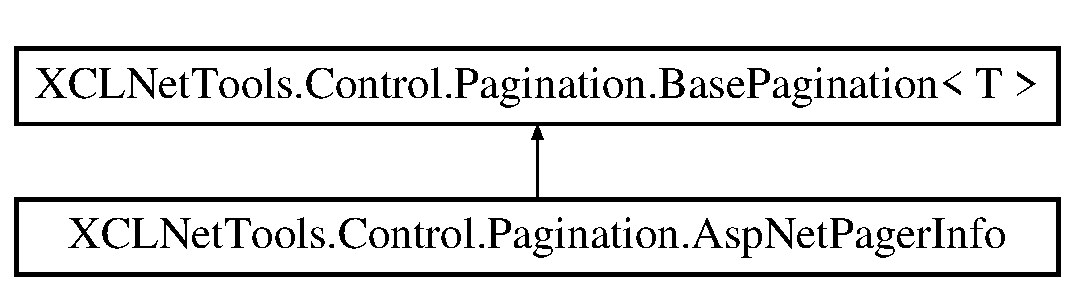
\includegraphics[height=2.000000cm]{class_x_c_l_net_tools_1_1_control_1_1_pagination_1_1_asp_net_pager_info}
\end{center}
\end{figure}
\subsection*{Public 成员函数}
\begin{DoxyCompactItemize}
\item 
\hyperlink{class_x_c_l_net_tools_1_1_control_1_1_pagination_1_1_asp_net_pager_info_aef75d024dd66cc9d75cd61d4dddcb27b}{Asp\-Net\-Pager\-Info} (Wuqi.\-Webdiyer.\-Asp\-Net\-Pager pager, int page\-Index, int page\-Size, int record\-Count)
\begin{DoxyCompactList}\small\item\em 构造函数 \end{DoxyCompactList}\item 
override void \hyperlink{class_x_c_l_net_tools_1_1_control_1_1_pagination_1_1_asp_net_pager_info_a46b208799b1d020c45571657c707ddf0}{Init\-Pager} ()
\begin{DoxyCompactList}\small\item\em 分页控件初始化 \end{DoxyCompactList}\end{DoxyCompactItemize}
\subsection*{额外继承的成员函数}


\subsection{详细描述}
Asp\-Net\-Pager分页 分页控件来源:http\-://www.webdiyer.\-com/aspnetpager/ 



在文件 Asp\-Net\-Pager\-Info.\-cs 第 15 行定义.



\subsection{构造及析构函数说明}
\hypertarget{class_x_c_l_net_tools_1_1_control_1_1_pagination_1_1_asp_net_pager_info_aef75d024dd66cc9d75cd61d4dddcb27b}{\index{X\-C\-L\-Net\-Tools\-::\-Control\-::\-Pagination\-::\-Asp\-Net\-Pager\-Info@{X\-C\-L\-Net\-Tools\-::\-Control\-::\-Pagination\-::\-Asp\-Net\-Pager\-Info}!Asp\-Net\-Pager\-Info@{Asp\-Net\-Pager\-Info}}
\index{Asp\-Net\-Pager\-Info@{Asp\-Net\-Pager\-Info}!XCLNetTools::Control::Pagination::AspNetPagerInfo@{X\-C\-L\-Net\-Tools\-::\-Control\-::\-Pagination\-::\-Asp\-Net\-Pager\-Info}}
\subsubsection[{Asp\-Net\-Pager\-Info}]{\setlength{\rightskip}{0pt plus 5cm}X\-C\-L\-Net\-Tools.\-Control.\-Pagination.\-Asp\-Net\-Pager\-Info.\-Asp\-Net\-Pager\-Info (
\begin{DoxyParamCaption}
\item[{Wuqi.\-Webdiyer.\-Asp\-Net\-Pager}]{pager, }
\item[{int}]{page\-Index, }
\item[{int}]{page\-Size, }
\item[{int}]{record\-Count}
\end{DoxyParamCaption}
)}}\label{class_x_c_l_net_tools_1_1_control_1_1_pagination_1_1_asp_net_pager_info_aef75d024dd66cc9d75cd61d4dddcb27b}


构造函数 


\begin{DoxyParams}{参数}
{\em pager} & 分页控件对象\\
\hline
{\em page\-Index} & 当前页码\\
\hline
{\em page\-Size} & 每页最多显示的记录数\\
\hline
{\em record\-Count} & 记录总数\\
\hline
\end{DoxyParams}


在文件 Asp\-Net\-Pager\-Info.\-cs 第 24 行定义.



\subsection{成员函数说明}
\hypertarget{class_x_c_l_net_tools_1_1_control_1_1_pagination_1_1_asp_net_pager_info_a46b208799b1d020c45571657c707ddf0}{\index{X\-C\-L\-Net\-Tools\-::\-Control\-::\-Pagination\-::\-Asp\-Net\-Pager\-Info@{X\-C\-L\-Net\-Tools\-::\-Control\-::\-Pagination\-::\-Asp\-Net\-Pager\-Info}!Init\-Pager@{Init\-Pager}}
\index{Init\-Pager@{Init\-Pager}!XCLNetTools::Control::Pagination::AspNetPagerInfo@{X\-C\-L\-Net\-Tools\-::\-Control\-::\-Pagination\-::\-Asp\-Net\-Pager\-Info}}
\subsubsection[{Init\-Pager}]{\setlength{\rightskip}{0pt plus 5cm}override void X\-C\-L\-Net\-Tools.\-Control.\-Pagination.\-Asp\-Net\-Pager\-Info.\-Init\-Pager (
\begin{DoxyParamCaption}
{}
\end{DoxyParamCaption}
)\hspace{0.3cm}{\ttfamily [virtual]}}}\label{class_x_c_l_net_tools_1_1_control_1_1_pagination_1_1_asp_net_pager_info_a46b208799b1d020c45571657c707ddf0}


分页控件初始化 



重载 \hyperlink{class_x_c_l_net_tools_1_1_control_1_1_pagination_1_1_base_pagination_3_01_t_01_4_ab3485196d5422f857f29f96bfbb2faa9}{X\-C\-L\-Net\-Tools.\-Control.\-Pagination.\-Base\-Pagination$<$ T $>$} .



在文件 Asp\-Net\-Pager\-Info.\-cs 第 32 行定义.



该类的文档由以下文件生成\-:\begin{DoxyCompactItemize}
\item 
D\-:/\-My\-Data/\-My\-Git/\-Git\-Hub/\-X\-C\-L\-Net\-Tools/\-X\-C\-L\-Net\-Tools/\-Control/\-Pagination/\hyperlink{_asp_net_pager_info_8cs}{Asp\-Net\-Pager\-Info.\-cs}\end{DoxyCompactItemize}

\hypertarget{class_x_c_l_net_tools_1_1_encode_1_1_base64}{}\section{X\+C\+L\+Net\+Tools.\+Encode.\+Base64类 参考}
\label{class_x_c_l_net_tools_1_1_encode_1_1_base64}\index{X\+C\+L\+Net\+Tools.\+Encode.\+Base64@{X\+C\+L\+Net\+Tools.\+Encode.\+Base64}}


base64相关  


\subsection*{静态 Public 成员函数}
\begin{DoxyCompactItemize}
\item 
static string \hyperlink{class_x_c_l_net_tools_1_1_encode_1_1_base64_a628c4b09c3625b12f0d4f76d3a16cf00}{Base64\+Code} (string msg)
\begin{DoxyCompactList}\small\item\em Base64加密 \end{DoxyCompactList}\item 
static string \hyperlink{class_x_c_l_net_tools_1_1_encode_1_1_base64_af51bea13594029540c9e9abf3ce1bfb2}{Base64\+Decode} (string msg)
\begin{DoxyCompactList}\small\item\em Base64解密 \end{DoxyCompactList}\end{DoxyCompactItemize}


\subsection{详细描述}
base64相关 



在文件 Base64.\+cs 第 17 行定义.



\subsection{成员函数说明}
\index{X\+C\+L\+Net\+Tools\+::\+Encode\+::\+Base64@{X\+C\+L\+Net\+Tools\+::\+Encode\+::\+Base64}!Base64\+Code@{Base64\+Code}}
\index{Base64\+Code@{Base64\+Code}!X\+C\+L\+Net\+Tools\+::\+Encode\+::\+Base64@{X\+C\+L\+Net\+Tools\+::\+Encode\+::\+Base64}}
\subsubsection[{\texorpdfstring{Base64\+Code(string msg)}{Base64Code(string msg)}}]{\setlength{\rightskip}{0pt plus 5cm}static string X\+C\+L\+Net\+Tools.\+Encode.\+Base64.\+Base64\+Code (
\begin{DoxyParamCaption}
\item[{string}]{msg}
\end{DoxyParamCaption}
)\hspace{0.3cm}{\ttfamily [static]}}\hypertarget{class_x_c_l_net_tools_1_1_encode_1_1_base64_a628c4b09c3625b12f0d4f76d3a16cf00}{}\label{class_x_c_l_net_tools_1_1_encode_1_1_base64_a628c4b09c3625b12f0d4f76d3a16cf00}


Base64加密 


\begin{DoxyParams}{参数}
{\em msg} & 要加密的内容\\
\hline
\end{DoxyParams}
\begin{DoxyReturn}{返回}
加密后的值
\end{DoxyReturn}


在文件 Base64.\+cs 第 24 行定义.

\index{X\+C\+L\+Net\+Tools\+::\+Encode\+::\+Base64@{X\+C\+L\+Net\+Tools\+::\+Encode\+::\+Base64}!Base64\+Decode@{Base64\+Decode}}
\index{Base64\+Decode@{Base64\+Decode}!X\+C\+L\+Net\+Tools\+::\+Encode\+::\+Base64@{X\+C\+L\+Net\+Tools\+::\+Encode\+::\+Base64}}
\subsubsection[{\texorpdfstring{Base64\+Decode(string msg)}{Base64Decode(string msg)}}]{\setlength{\rightskip}{0pt plus 5cm}static string X\+C\+L\+Net\+Tools.\+Encode.\+Base64.\+Base64\+Decode (
\begin{DoxyParamCaption}
\item[{string}]{msg}
\end{DoxyParamCaption}
)\hspace{0.3cm}{\ttfamily [static]}}\hypertarget{class_x_c_l_net_tools_1_1_encode_1_1_base64_af51bea13594029540c9e9abf3ce1bfb2}{}\label{class_x_c_l_net_tools_1_1_encode_1_1_base64_af51bea13594029540c9e9abf3ce1bfb2}


Base64解密 


\begin{DoxyParams}{参数}
{\em msg} & 要解密的内容\\
\hline
\end{DoxyParams}
\begin{DoxyReturn}{返回}
解密后的值
\end{DoxyReturn}


在文件 Base64.\+cs 第 35 行定义.



该类的文档由以下文件生成\+:\begin{DoxyCompactItemize}
\item 
E\+:/\+Git\+Hub/\+X\+C\+L\+Net\+Tools/\+X\+C\+L\+Net\+Tools/\+Encode/\hyperlink{_base64_8cs}{Base64.\+cs}\end{DoxyCompactItemize}

\hypertarget{class_x_c_l_net_tools_1_1_control_1_1_pagination_1_1_base_pagination_3_01_t_01_4}{\section{X\-C\-L\-Net\-Tools.\-Control.\-Pagination.\-Base\-Pagination$<$ T $>$ 模板类 参考}
\label{class_x_c_l_net_tools_1_1_control_1_1_pagination_1_1_base_pagination_3_01_t_01_4}\index{X\-C\-L\-Net\-Tools.\-Control.\-Pagination.\-Base\-Pagination$<$ T $>$@{X\-C\-L\-Net\-Tools.\-Control.\-Pagination.\-Base\-Pagination$<$ T $>$}}
}


分页抽象类  


类 X\-C\-L\-Net\-Tools.\-Control.\-Pagination.\-Base\-Pagination$<$ T $>$ 继承关系图\-:\begin{figure}[H]
\begin{center}
\leavevmode
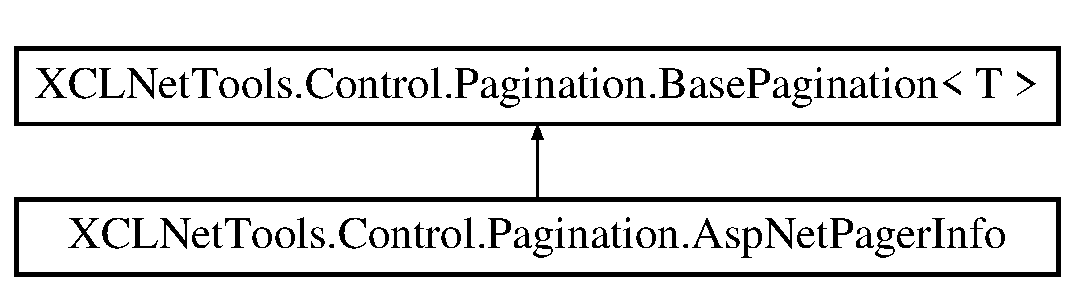
\includegraphics[height=2.000000cm]{class_x_c_l_net_tools_1_1_control_1_1_pagination_1_1_base_pagination_3_01_t_01_4}
\end{center}
\end{figure}
\subsection*{Public 成员函数}
\begin{DoxyCompactItemize}
\item 
\hyperlink{class_x_c_l_net_tools_1_1_control_1_1_pagination_1_1_base_pagination_3_01_t_01_4_ae9e336c1452804e7d4de12ea9fa3ddde}{Base\-Pagination} (T pager, int page\-Index, int page\-Size, int record\-Count)
\begin{DoxyCompactList}\small\item\em 构造函数 \end{DoxyCompactList}\item 
virtual void \hyperlink{class_x_c_l_net_tools_1_1_control_1_1_pagination_1_1_base_pagination_3_01_t_01_4_ab3485196d5422f857f29f96bfbb2faa9}{Init\-Pager} ()
\begin{DoxyCompactList}\small\item\em 分页初始化 \end{DoxyCompactList}\end{DoxyCompactItemize}
\subsection*{属性}
\begin{DoxyCompactItemize}
\item 
T \hyperlink{class_x_c_l_net_tools_1_1_control_1_1_pagination_1_1_base_pagination_3_01_t_01_4_ae0cfdba3ea23387da4b851c4d695d0a0}{Pager}\hspace{0.3cm}{\ttfamily  \mbox{[}get, set\mbox{]}}
\begin{DoxyCompactList}\small\item\em 当前分页控件 \end{DoxyCompactList}\item 
\hyperlink{class_x_c_l_net_tools_1_1_entity_1_1_pager_info}{X\-C\-L\-Net\-Tools.\-Entity.\-Pager\-Info} \hyperlink{class_x_c_l_net_tools_1_1_control_1_1_pagination_1_1_base_pagination_3_01_t_01_4_ae27d645cd692bb7471bc6236c59496a3}{Pager\-Info}\hspace{0.3cm}{\ttfamily  \mbox{[}get, set\mbox{]}}
\begin{DoxyCompactList}\small\item\em 分页信息 \end{DoxyCompactList}\end{DoxyCompactItemize}


\subsection{详细描述}
分页抽象类 



在文件 Base\-Pagination.\-cs 第 30 行定义.



\subsection{构造及析构函数说明}
\hypertarget{class_x_c_l_net_tools_1_1_control_1_1_pagination_1_1_base_pagination_3_01_t_01_4_ae9e336c1452804e7d4de12ea9fa3ddde}{\index{X\-C\-L\-Net\-Tools\-::\-Control\-::\-Pagination\-::\-Base\-Pagination$<$ T $>$@{X\-C\-L\-Net\-Tools\-::\-Control\-::\-Pagination\-::\-Base\-Pagination$<$ T $>$}!Base\-Pagination@{Base\-Pagination}}
\index{Base\-Pagination@{Base\-Pagination}!XCLNetTools::Control::Pagination::BasePagination< T >@{X\-C\-L\-Net\-Tools\-::\-Control\-::\-Pagination\-::\-Base\-Pagination$<$ T $>$}}
\subsubsection[{Base\-Pagination}]{\setlength{\rightskip}{0pt plus 5cm}X\-C\-L\-Net\-Tools.\-Control.\-Pagination.\-Base\-Pagination$<$ T $>$.Base\-Pagination (
\begin{DoxyParamCaption}
\item[{T}]{pager, }
\item[{int}]{page\-Index, }
\item[{int}]{page\-Size, }
\item[{int}]{record\-Count}
\end{DoxyParamCaption}
)}}\label{class_x_c_l_net_tools_1_1_control_1_1_pagination_1_1_base_pagination_3_01_t_01_4_ae9e336c1452804e7d4de12ea9fa3ddde}


构造函数 


\begin{DoxyParams}{参数}
{\em pager} & 分页控件对象\\
\hline
{\em page\-Index} & 当前页码\\
\hline
{\em page\-Size} & 每页最多显示的记录数\\
\hline
{\em record\-Count} & 记录总数\\
\hline
\end{DoxyParams}


在文件 Base\-Pagination.\-cs 第 43 行定义.



\subsection{成员函数说明}
\hypertarget{class_x_c_l_net_tools_1_1_control_1_1_pagination_1_1_base_pagination_3_01_t_01_4_ab3485196d5422f857f29f96bfbb2faa9}{\index{X\-C\-L\-Net\-Tools\-::\-Control\-::\-Pagination\-::\-Base\-Pagination$<$ T $>$@{X\-C\-L\-Net\-Tools\-::\-Control\-::\-Pagination\-::\-Base\-Pagination$<$ T $>$}!Init\-Pager@{Init\-Pager}}
\index{Init\-Pager@{Init\-Pager}!XCLNetTools::Control::Pagination::BasePagination< T >@{X\-C\-L\-Net\-Tools\-::\-Control\-::\-Pagination\-::\-Base\-Pagination$<$ T $>$}}
\subsubsection[{Init\-Pager}]{\setlength{\rightskip}{0pt plus 5cm}virtual void X\-C\-L\-Net\-Tools.\-Control.\-Pagination.\-Base\-Pagination$<$ T $>$.Init\-Pager (
\begin{DoxyParamCaption}
{}
\end{DoxyParamCaption}
)\hspace{0.3cm}{\ttfamily [virtual]}}}\label{class_x_c_l_net_tools_1_1_control_1_1_pagination_1_1_base_pagination_3_01_t_01_4_ab3485196d5422f857f29f96bfbb2faa9}


分页初始化 



被 \hyperlink{class_x_c_l_net_tools_1_1_control_1_1_pagination_1_1_asp_net_pager_info_a46b208799b1d020c45571657c707ddf0}{X\-C\-L\-Net\-Tools.\-Control.\-Pagination.\-Asp\-Net\-Pager\-Info} 重载.



在文件 Base\-Pagination.\-cs 第 63 行定义.



\subsection{属性说明}
\hypertarget{class_x_c_l_net_tools_1_1_control_1_1_pagination_1_1_base_pagination_3_01_t_01_4_ae0cfdba3ea23387da4b851c4d695d0a0}{\index{X\-C\-L\-Net\-Tools\-::\-Control\-::\-Pagination\-::\-Base\-Pagination$<$ T $>$@{X\-C\-L\-Net\-Tools\-::\-Control\-::\-Pagination\-::\-Base\-Pagination$<$ T $>$}!Pager@{Pager}}
\index{Pager@{Pager}!XCLNetTools::Control::Pagination::BasePagination< T >@{X\-C\-L\-Net\-Tools\-::\-Control\-::\-Pagination\-::\-Base\-Pagination$<$ T $>$}}
\subsubsection[{Pager}]{\setlength{\rightskip}{0pt plus 5cm}T X\-C\-L\-Net\-Tools.\-Control.\-Pagination.\-Base\-Pagination$<$ T $>$.Pager\hspace{0.3cm}{\ttfamily [get]}, {\ttfamily [set]}}}\label{class_x_c_l_net_tools_1_1_control_1_1_pagination_1_1_base_pagination_3_01_t_01_4_ae0cfdba3ea23387da4b851c4d695d0a0}


当前分页控件 



在文件 Base\-Pagination.\-cs 第 53 行定义.

\hypertarget{class_x_c_l_net_tools_1_1_control_1_1_pagination_1_1_base_pagination_3_01_t_01_4_ae27d645cd692bb7471bc6236c59496a3}{\index{X\-C\-L\-Net\-Tools\-::\-Control\-::\-Pagination\-::\-Base\-Pagination$<$ T $>$@{X\-C\-L\-Net\-Tools\-::\-Control\-::\-Pagination\-::\-Base\-Pagination$<$ T $>$}!Pager\-Info@{Pager\-Info}}
\index{Pager\-Info@{Pager\-Info}!XCLNetTools::Control::Pagination::BasePagination< T >@{X\-C\-L\-Net\-Tools\-::\-Control\-::\-Pagination\-::\-Base\-Pagination$<$ T $>$}}
\subsubsection[{Pager\-Info}]{\setlength{\rightskip}{0pt plus 5cm}{\bf X\-C\-L\-Net\-Tools.\-Entity.\-Pager\-Info} X\-C\-L\-Net\-Tools.\-Control.\-Pagination.\-Base\-Pagination$<$ T $>$.Pager\-Info\hspace{0.3cm}{\ttfamily [get]}, {\ttfamily [set]}}}\label{class_x_c_l_net_tools_1_1_control_1_1_pagination_1_1_base_pagination_3_01_t_01_4_ae27d645cd692bb7471bc6236c59496a3}


分页信息 



在文件 Base\-Pagination.\-cs 第 58 行定义.



该类的文档由以下文件生成\-:\begin{DoxyCompactItemize}
\item 
D\-:/\-My\-Data/\-My\-Git/\-Git\-Hub/\-X\-C\-L\-Net\-Tools/\-X\-C\-L\-Net\-Tools/\-Control/\-Pagination/\hyperlink{_base_pagination_8cs}{Base\-Pagination.\-cs}\end{DoxyCompactItemize}

\hypertarget{class_x_c_l_net_tools_1_1_file_handler_1_1_bookmark}{}\section{X\+C\+L\+Net\+Tools.\+File\+Handler.\+Bookmark类 参考}
\label{class_x_c_l_net_tools_1_1_file_handler_1_1_bookmark}\index{X\+C\+L\+Net\+Tools.\+File\+Handler.\+Bookmark@{X\+C\+L\+Net\+Tools.\+File\+Handler.\+Bookmark}}


浏览器书签文件操作类  


\subsection*{静态 Public 成员函数}
\begin{DoxyCompactItemize}
\item 
static List$<$ \hyperlink{class_x_c_l_net_tools_1_1_entity_1_1_bookmark_entity}{X\+C\+L\+Net\+Tools.\+Entity.\+Bookmark\+Entity} $>$ \hyperlink{class_x_c_l_net_tools_1_1_file_handler_1_1_bookmark_ab84885635ae274703936c5c10ae0f67c}{Get\+Bookmark} (string path)
\begin{DoxyCompactList}\small\item\em 根据浏览器书签文件地址,返回list \end{DoxyCompactList}\end{DoxyCompactItemize}


\subsection{详细描述}
浏览器书签文件操作类 



在文件 Bookmark.\+cs 第 18 行定义.



\subsection{成员函数说明}
\mbox{\Hypertarget{class_x_c_l_net_tools_1_1_file_handler_1_1_bookmark_ab84885635ae274703936c5c10ae0f67c}\label{class_x_c_l_net_tools_1_1_file_handler_1_1_bookmark_ab84885635ae274703936c5c10ae0f67c}} 
\index{X\+C\+L\+Net\+Tools\+::\+File\+Handler\+::\+Bookmark@{X\+C\+L\+Net\+Tools\+::\+File\+Handler\+::\+Bookmark}!Get\+Bookmark@{Get\+Bookmark}}
\index{Get\+Bookmark@{Get\+Bookmark}!X\+C\+L\+Net\+Tools\+::\+File\+Handler\+::\+Bookmark@{X\+C\+L\+Net\+Tools\+::\+File\+Handler\+::\+Bookmark}}
\subsubsection{\texorpdfstring{Get\+Bookmark()}{GetBookmark()}}
{\footnotesize\ttfamily static List$<$\hyperlink{class_x_c_l_net_tools_1_1_entity_1_1_bookmark_entity}{X\+C\+L\+Net\+Tools.\+Entity.\+Bookmark\+Entity}$>$ X\+C\+L\+Net\+Tools.\+File\+Handler.\+Bookmark.\+Get\+Bookmark (\begin{DoxyParamCaption}\item[{string}]{path }\end{DoxyParamCaption})\hspace{0.3cm}{\ttfamily [static]}}



根据浏览器书签文件地址,返回list 


\begin{DoxyParams}{参数}
{\em path} & 书签文件地址\\
\hline
\end{DoxyParams}
\begin{DoxyReturn}{返回}
书签list
\end{DoxyReturn}


在文件 Bookmark.\+cs 第 25 行定义.



该类的文档由以下文件生成\+:\begin{DoxyCompactItemize}
\item 
D\+:/\+My\+Data/\+Git\+Hub/\+X\+C\+L\+Net\+Tools/\+X\+C\+L\+Net\+Tools/\+File\+Handler/\hyperlink{_bookmark_8cs}{Bookmark.\+cs}\end{DoxyCompactItemize}

\hypertarget{class_x_c_l_net_tools_1_1_entity_1_1_bookmark_entity}{}\section{X\+C\+L\+Net\+Tools.\+Entity.\+Bookmark\+Entity类 参考}
\label{class_x_c_l_net_tools_1_1_entity_1_1_bookmark_entity}\index{X\+C\+L\+Net\+Tools.\+Entity.\+Bookmark\+Entity@{X\+C\+L\+Net\+Tools.\+Entity.\+Bookmark\+Entity}}


浏览器书签实体  


\subsection*{属性}
\begin{DoxyCompactItemize}
\item 
int \hyperlink{class_x_c_l_net_tools_1_1_entity_1_1_bookmark_entity_a827314c81aad0801f464f7359509baec}{Id}\hspace{0.3cm}{\ttfamily  \mbox{[}get, set\mbox{]}}
\begin{DoxyCompactList}\small\item\em 编号 \end{DoxyCompactList}\item 
int \hyperlink{class_x_c_l_net_tools_1_1_entity_1_1_bookmark_entity_afd3c2002aa8d5edeac06f6ef32ba7454}{Parent\+Id}\hspace{0.3cm}{\ttfamily  \mbox{[}get, set\mbox{]}}
\begin{DoxyCompactList}\small\item\em 父id \end{DoxyCompactList}\item 
bool \hyperlink{class_x_c_l_net_tools_1_1_entity_1_1_bookmark_entity_a025f1606c5b38103058567b3e08afe03}{Is\+Folder}\hspace{0.3cm}{\ttfamily  \mbox{[}get, set\mbox{]}}
\begin{DoxyCompactList}\small\item\em 是否为文件夹 \end{DoxyCompactList}\item 
string \hyperlink{class_x_c_l_net_tools_1_1_entity_1_1_bookmark_entity_a89ccb517e285bfdd17981a72f590bc1c}{Name}\hspace{0.3cm}{\ttfamily  \mbox{[}get, set\mbox{]}}
\begin{DoxyCompactList}\small\item\em 书签名称 \end{DoxyCompactList}\item 
string \hyperlink{class_x_c_l_net_tools_1_1_entity_1_1_bookmark_entity_af370dbfd32e8cde501e305c6999c077b}{Ico\+U\+RL}\hspace{0.3cm}{\ttfamily  \mbox{[}get, set\mbox{]}}
\begin{DoxyCompactList}\small\item\em ico图标地址 \end{DoxyCompactList}\item 
string \hyperlink{class_x_c_l_net_tools_1_1_entity_1_1_bookmark_entity_a88ebfe2441fd5804a82f5eaee1ce3232}{Url}\hspace{0.3cm}{\ttfamily  \mbox{[}get, set\mbox{]}}
\begin{DoxyCompactList}\small\item\em 书签链接 \end{DoxyCompactList}\end{DoxyCompactItemize}


\subsection{详细描述}
浏览器书签实体 



在文件 Bookmark\+Entity.\+cs 第 17 行定义.



\subsection{属性说明}
\index{X\+C\+L\+Net\+Tools\+::\+Entity\+::\+Bookmark\+Entity@{X\+C\+L\+Net\+Tools\+::\+Entity\+::\+Bookmark\+Entity}!Ico\+U\+RL@{Ico\+U\+RL}}
\index{Ico\+U\+RL@{Ico\+U\+RL}!X\+C\+L\+Net\+Tools\+::\+Entity\+::\+Bookmark\+Entity@{X\+C\+L\+Net\+Tools\+::\+Entity\+::\+Bookmark\+Entity}}
\subsubsection[{\texorpdfstring{Ico\+U\+RL}{IcoURL}}]{\setlength{\rightskip}{0pt plus 5cm}string X\+C\+L\+Net\+Tools.\+Entity.\+Bookmark\+Entity.\+Ico\+U\+RL\hspace{0.3cm}{\ttfamily [get]}, {\ttfamily [set]}}\hypertarget{class_x_c_l_net_tools_1_1_entity_1_1_bookmark_entity_af370dbfd32e8cde501e305c6999c077b}{}\label{class_x_c_l_net_tools_1_1_entity_1_1_bookmark_entity_af370dbfd32e8cde501e305c6999c077b}


ico图标地址 



在文件 Bookmark\+Entity.\+cs 第 42 行定义.

\index{X\+C\+L\+Net\+Tools\+::\+Entity\+::\+Bookmark\+Entity@{X\+C\+L\+Net\+Tools\+::\+Entity\+::\+Bookmark\+Entity}!Id@{Id}}
\index{Id@{Id}!X\+C\+L\+Net\+Tools\+::\+Entity\+::\+Bookmark\+Entity@{X\+C\+L\+Net\+Tools\+::\+Entity\+::\+Bookmark\+Entity}}
\subsubsection[{\texorpdfstring{Id}{Id}}]{\setlength{\rightskip}{0pt plus 5cm}int X\+C\+L\+Net\+Tools.\+Entity.\+Bookmark\+Entity.\+Id\hspace{0.3cm}{\ttfamily [get]}, {\ttfamily [set]}}\hypertarget{class_x_c_l_net_tools_1_1_entity_1_1_bookmark_entity_a827314c81aad0801f464f7359509baec}{}\label{class_x_c_l_net_tools_1_1_entity_1_1_bookmark_entity_a827314c81aad0801f464f7359509baec}


编号 



在文件 Bookmark\+Entity.\+cs 第 22 行定义.

\index{X\+C\+L\+Net\+Tools\+::\+Entity\+::\+Bookmark\+Entity@{X\+C\+L\+Net\+Tools\+::\+Entity\+::\+Bookmark\+Entity}!Is\+Folder@{Is\+Folder}}
\index{Is\+Folder@{Is\+Folder}!X\+C\+L\+Net\+Tools\+::\+Entity\+::\+Bookmark\+Entity@{X\+C\+L\+Net\+Tools\+::\+Entity\+::\+Bookmark\+Entity}}
\subsubsection[{\texorpdfstring{Is\+Folder}{IsFolder}}]{\setlength{\rightskip}{0pt plus 5cm}bool X\+C\+L\+Net\+Tools.\+Entity.\+Bookmark\+Entity.\+Is\+Folder\hspace{0.3cm}{\ttfamily [get]}, {\ttfamily [set]}}\hypertarget{class_x_c_l_net_tools_1_1_entity_1_1_bookmark_entity_a025f1606c5b38103058567b3e08afe03}{}\label{class_x_c_l_net_tools_1_1_entity_1_1_bookmark_entity_a025f1606c5b38103058567b3e08afe03}


是否为文件夹 



在文件 Bookmark\+Entity.\+cs 第 32 行定义.

\index{X\+C\+L\+Net\+Tools\+::\+Entity\+::\+Bookmark\+Entity@{X\+C\+L\+Net\+Tools\+::\+Entity\+::\+Bookmark\+Entity}!Name@{Name}}
\index{Name@{Name}!X\+C\+L\+Net\+Tools\+::\+Entity\+::\+Bookmark\+Entity@{X\+C\+L\+Net\+Tools\+::\+Entity\+::\+Bookmark\+Entity}}
\subsubsection[{\texorpdfstring{Name}{Name}}]{\setlength{\rightskip}{0pt plus 5cm}string X\+C\+L\+Net\+Tools.\+Entity.\+Bookmark\+Entity.\+Name\hspace{0.3cm}{\ttfamily [get]}, {\ttfamily [set]}}\hypertarget{class_x_c_l_net_tools_1_1_entity_1_1_bookmark_entity_a89ccb517e285bfdd17981a72f590bc1c}{}\label{class_x_c_l_net_tools_1_1_entity_1_1_bookmark_entity_a89ccb517e285bfdd17981a72f590bc1c}


书签名称 



在文件 Bookmark\+Entity.\+cs 第 37 行定义.

\index{X\+C\+L\+Net\+Tools\+::\+Entity\+::\+Bookmark\+Entity@{X\+C\+L\+Net\+Tools\+::\+Entity\+::\+Bookmark\+Entity}!Parent\+Id@{Parent\+Id}}
\index{Parent\+Id@{Parent\+Id}!X\+C\+L\+Net\+Tools\+::\+Entity\+::\+Bookmark\+Entity@{X\+C\+L\+Net\+Tools\+::\+Entity\+::\+Bookmark\+Entity}}
\subsubsection[{\texorpdfstring{Parent\+Id}{ParentId}}]{\setlength{\rightskip}{0pt plus 5cm}int X\+C\+L\+Net\+Tools.\+Entity.\+Bookmark\+Entity.\+Parent\+Id\hspace{0.3cm}{\ttfamily [get]}, {\ttfamily [set]}}\hypertarget{class_x_c_l_net_tools_1_1_entity_1_1_bookmark_entity_afd3c2002aa8d5edeac06f6ef32ba7454}{}\label{class_x_c_l_net_tools_1_1_entity_1_1_bookmark_entity_afd3c2002aa8d5edeac06f6ef32ba7454}


父id 



在文件 Bookmark\+Entity.\+cs 第 27 行定义.

\index{X\+C\+L\+Net\+Tools\+::\+Entity\+::\+Bookmark\+Entity@{X\+C\+L\+Net\+Tools\+::\+Entity\+::\+Bookmark\+Entity}!Url@{Url}}
\index{Url@{Url}!X\+C\+L\+Net\+Tools\+::\+Entity\+::\+Bookmark\+Entity@{X\+C\+L\+Net\+Tools\+::\+Entity\+::\+Bookmark\+Entity}}
\subsubsection[{\texorpdfstring{Url}{Url}}]{\setlength{\rightskip}{0pt plus 5cm}string X\+C\+L\+Net\+Tools.\+Entity.\+Bookmark\+Entity.\+Url\hspace{0.3cm}{\ttfamily [get]}, {\ttfamily [set]}}\hypertarget{class_x_c_l_net_tools_1_1_entity_1_1_bookmark_entity_a88ebfe2441fd5804a82f5eaee1ce3232}{}\label{class_x_c_l_net_tools_1_1_entity_1_1_bookmark_entity_a88ebfe2441fd5804a82f5eaee1ce3232}


书签链接 



在文件 Bookmark\+Entity.\+cs 第 47 行定义.



该类的文档由以下文件生成\+:\begin{DoxyCompactItemize}
\item 
E\+:/\+Git\+Hub/\+X\+C\+L\+Net\+Tools/\+X\+C\+L\+Net\+Tools/\+Entity/\hyperlink{_bookmark_entity_8cs}{Bookmark\+Entity.\+cs}\end{DoxyCompactItemize}

\hypertarget{class_x_c_l_net_tools_1_1_cache_1_1_cache_class}{\section{X\-C\-L\-Net\-Tools.\-Cache.\-Cache\-Class类 参考}
\label{class_x_c_l_net_tools_1_1_cache_1_1_cache_class}\index{X\-C\-L\-Net\-Tools.\-Cache.\-Cache\-Class@{X\-C\-L\-Net\-Tools.\-Cache.\-Cache\-Class}}
}


缓存相关的操作类  


\subsection*{静态 Public 成员函数}
\begin{DoxyCompactItemize}
\item 
static object \hyperlink{class_x_c_l_net_tools_1_1_cache_1_1_cache_class_aa4eb429181d14c79040ea957bb4b8308}{Get\-Cache} (string Cache\-Key)
\begin{DoxyCompactList}\small\item\em 获取当前应用程序指定\-Cache\-Key的\-Cache值 \end{DoxyCompactList}\item 
static void \hyperlink{class_x_c_l_net_tools_1_1_cache_1_1_cache_class_a1f815a266c55067bab54e36c276ea82b}{Set\-Cache} (string Cache\-Key, object obj\-Object)
\begin{DoxyCompactList}\small\item\em 设置当前应用程序指定\-Cache\-Key的\-Cache值 \end{DoxyCompactList}\item 
static void \hyperlink{class_x_c_l_net_tools_1_1_cache_1_1_cache_class_a12454bcf0c4d79e76937bbd927df631e}{Set\-Cache} (string Cache\-Key, object obj\-Object, Date\-Time absolute\-Expiration, Time\-Span sliding\-Expiration)
\begin{DoxyCompactList}\small\item\em 设置当前应用程序指定\-Cache\-Key的\-Cache值 \end{DoxyCompactList}\item 
static void \hyperlink{class_x_c_l_net_tools_1_1_cache_1_1_cache_class_afeab3c01d1a7b41007235b97f3fbaa35}{Clear} (string key)
\begin{DoxyCompactList}\small\item\em 删除指定缓存 \end{DoxyCompactList}\item 
static bool \hyperlink{class_x_c_l_net_tools_1_1_cache_1_1_cache_class_aa7640102a9327d10ff130c69b724e27b}{Exists} (string key)
\begin{DoxyCompactList}\small\item\em 指定缓存是否存在 \end{DoxyCompactList}\item 
static void \hyperlink{class_x_c_l_net_tools_1_1_cache_1_1_cache_class_a36ade93bd935dbad5740285d48e2c5e6}{Remove\-All\-Cache} ()
\begin{DoxyCompactList}\small\item\em 移除全部缓存 \end{DoxyCompactList}\end{DoxyCompactItemize}


\subsection{详细描述}
缓存相关的操作类 



在文件 Cache\-Class.\-cs 第 34 行定义.



\subsection{成员函数说明}
\hypertarget{class_x_c_l_net_tools_1_1_cache_1_1_cache_class_afeab3c01d1a7b41007235b97f3fbaa35}{\index{X\-C\-L\-Net\-Tools\-::\-Cache\-::\-Cache\-Class@{X\-C\-L\-Net\-Tools\-::\-Cache\-::\-Cache\-Class}!Clear@{Clear}}
\index{Clear@{Clear}!XCLNetTools::Cache::CacheClass@{X\-C\-L\-Net\-Tools\-::\-Cache\-::\-Cache\-Class}}
\subsubsection[{Clear}]{\setlength{\rightskip}{0pt plus 5cm}static void X\-C\-L\-Net\-Tools.\-Cache.\-Cache\-Class.\-Clear (
\begin{DoxyParamCaption}
\item[{string}]{key}
\end{DoxyParamCaption}
)\hspace{0.3cm}{\ttfamily [static]}}}\label{class_x_c_l_net_tools_1_1_cache_1_1_cache_class_afeab3c01d1a7b41007235b97f3fbaa35}


删除指定缓存 


\begin{DoxyParams}{参数}
{\em key} & 缓存key名\\
\hline
\end{DoxyParams}


在文件 Cache\-Class.\-cs 第 72 行定义.

\hypertarget{class_x_c_l_net_tools_1_1_cache_1_1_cache_class_aa7640102a9327d10ff130c69b724e27b}{\index{X\-C\-L\-Net\-Tools\-::\-Cache\-::\-Cache\-Class@{X\-C\-L\-Net\-Tools\-::\-Cache\-::\-Cache\-Class}!Exists@{Exists}}
\index{Exists@{Exists}!XCLNetTools::Cache::CacheClass@{X\-C\-L\-Net\-Tools\-::\-Cache\-::\-Cache\-Class}}
\subsubsection[{Exists}]{\setlength{\rightskip}{0pt plus 5cm}static bool X\-C\-L\-Net\-Tools.\-Cache.\-Cache\-Class.\-Exists (
\begin{DoxyParamCaption}
\item[{string}]{key}
\end{DoxyParamCaption}
)\hspace{0.3cm}{\ttfamily [static]}}}\label{class_x_c_l_net_tools_1_1_cache_1_1_cache_class_aa7640102a9327d10ff130c69b724e27b}


指定缓存是否存在 


\begin{DoxyParams}{参数}
{\em key} & 缓存名\\
\hline
\end{DoxyParams}
\begin{DoxyReturn}{返回}
true\-:存在
\end{DoxyReturn}


在文件 Cache\-Class.\-cs 第 82 行定义.

\hypertarget{class_x_c_l_net_tools_1_1_cache_1_1_cache_class_aa4eb429181d14c79040ea957bb4b8308}{\index{X\-C\-L\-Net\-Tools\-::\-Cache\-::\-Cache\-Class@{X\-C\-L\-Net\-Tools\-::\-Cache\-::\-Cache\-Class}!Get\-Cache@{Get\-Cache}}
\index{Get\-Cache@{Get\-Cache}!XCLNetTools::Cache::CacheClass@{X\-C\-L\-Net\-Tools\-::\-Cache\-::\-Cache\-Class}}
\subsubsection[{Get\-Cache}]{\setlength{\rightskip}{0pt plus 5cm}static object X\-C\-L\-Net\-Tools.\-Cache.\-Cache\-Class.\-Get\-Cache (
\begin{DoxyParamCaption}
\item[{string}]{Cache\-Key}
\end{DoxyParamCaption}
)\hspace{0.3cm}{\ttfamily [static]}}}\label{class_x_c_l_net_tools_1_1_cache_1_1_cache_class_aa4eb429181d14c79040ea957bb4b8308}


获取当前应用程序指定\-Cache\-Key的\-Cache值 


\begin{DoxyParams}{参数}
{\em Cache\-Key} & 缓存key名\\
\hline
\end{DoxyParams}
\begin{DoxyReturn}{返回}
该缓存的值
\end{DoxyReturn}


在文件 Cache\-Class.\-cs 第 41 行定义.

\hypertarget{class_x_c_l_net_tools_1_1_cache_1_1_cache_class_a36ade93bd935dbad5740285d48e2c5e6}{\index{X\-C\-L\-Net\-Tools\-::\-Cache\-::\-Cache\-Class@{X\-C\-L\-Net\-Tools\-::\-Cache\-::\-Cache\-Class}!Remove\-All\-Cache@{Remove\-All\-Cache}}
\index{Remove\-All\-Cache@{Remove\-All\-Cache}!XCLNetTools::Cache::CacheClass@{X\-C\-L\-Net\-Tools\-::\-Cache\-::\-Cache\-Class}}
\subsubsection[{Remove\-All\-Cache}]{\setlength{\rightskip}{0pt plus 5cm}static void X\-C\-L\-Net\-Tools.\-Cache.\-Cache\-Class.\-Remove\-All\-Cache (
\begin{DoxyParamCaption}
{}
\end{DoxyParamCaption}
)\hspace{0.3cm}{\ttfamily [static]}}}\label{class_x_c_l_net_tools_1_1_cache_1_1_cache_class_a36ade93bd935dbad5740285d48e2c5e6}


移除全部缓存 



在文件 Cache\-Class.\-cs 第 90 行定义.

\hypertarget{class_x_c_l_net_tools_1_1_cache_1_1_cache_class_a1f815a266c55067bab54e36c276ea82b}{\index{X\-C\-L\-Net\-Tools\-::\-Cache\-::\-Cache\-Class@{X\-C\-L\-Net\-Tools\-::\-Cache\-::\-Cache\-Class}!Set\-Cache@{Set\-Cache}}
\index{Set\-Cache@{Set\-Cache}!XCLNetTools::Cache::CacheClass@{X\-C\-L\-Net\-Tools\-::\-Cache\-::\-Cache\-Class}}
\subsubsection[{Set\-Cache}]{\setlength{\rightskip}{0pt plus 5cm}static void X\-C\-L\-Net\-Tools.\-Cache.\-Cache\-Class.\-Set\-Cache (
\begin{DoxyParamCaption}
\item[{string}]{Cache\-Key, }
\item[{object}]{obj\-Object}
\end{DoxyParamCaption}
)\hspace{0.3cm}{\ttfamily [static]}}}\label{class_x_c_l_net_tools_1_1_cache_1_1_cache_class_a1f815a266c55067bab54e36c276ea82b}


设置当前应用程序指定\-Cache\-Key的\-Cache值 


\begin{DoxyParams}{参数}
{\em Cache\-Key} & 缓存key名\\
\hline
{\em obj\-Object} & 缓存key值\\
\hline
\end{DoxyParams}


在文件 Cache\-Class.\-cs 第 51 行定义.

\hypertarget{class_x_c_l_net_tools_1_1_cache_1_1_cache_class_a12454bcf0c4d79e76937bbd927df631e}{\index{X\-C\-L\-Net\-Tools\-::\-Cache\-::\-Cache\-Class@{X\-C\-L\-Net\-Tools\-::\-Cache\-::\-Cache\-Class}!Set\-Cache@{Set\-Cache}}
\index{Set\-Cache@{Set\-Cache}!XCLNetTools::Cache::CacheClass@{X\-C\-L\-Net\-Tools\-::\-Cache\-::\-Cache\-Class}}
\subsubsection[{Set\-Cache}]{\setlength{\rightskip}{0pt plus 5cm}static void X\-C\-L\-Net\-Tools.\-Cache.\-Cache\-Class.\-Set\-Cache (
\begin{DoxyParamCaption}
\item[{string}]{Cache\-Key, }
\item[{object}]{obj\-Object, }
\item[{Date\-Time}]{absolute\-Expiration, }
\item[{Time\-Span}]{sliding\-Expiration}
\end{DoxyParamCaption}
)\hspace{0.3cm}{\ttfamily [static]}}}\label{class_x_c_l_net_tools_1_1_cache_1_1_cache_class_a12454bcf0c4d79e76937bbd927df631e}


设置当前应用程序指定\-Cache\-Key的\-Cache值 


\begin{DoxyParams}{参数}
{\em Cache\-Key} & 缓存key名\\
\hline
{\em obj\-Object} & 缓存key值\\
\hline
{\em absolute\-Expiration} & 所插入对象将到期并被从缓存中移除的时间\\
\hline
{\em sliding\-Expiration} & 最后一次访问所插入对象时与该对象到期时之间的时间间隔\\
\hline
\end{DoxyParams}


在文件 Cache\-Class.\-cs 第 63 行定义.



该类的文档由以下文件生成\-:\begin{DoxyCompactItemize}
\item 
D\-:/\-My\-Data/\-My\-Git/\-Git\-Hub/\-X\-C\-L\-Net\-Tools/\-X\-C\-L\-Net\-Tools/\-Cache/\hyperlink{_cache_class_8cs}{Cache\-Class.\-cs}\end{DoxyCompactItemize}

\hypertarget{class_x_c_l_net_tools_1_1_language_1_1_c_n}{\section{X\-C\-L\-Net\-Tools.\-Language.\-C\-N类 参考}
\label{class_x_c_l_net_tools_1_1_language_1_1_c_n}\index{X\-C\-L\-Net\-Tools.\-Language.\-C\-N@{X\-C\-L\-Net\-Tools.\-Language.\-C\-N}}
}


中文处理  


\subsection*{静态 Public 成员函数}
\begin{DoxyCompactItemize}
\item 
static string \hyperlink{class_x_c_l_net_tools_1_1_language_1_1_c_n_a298b6a886b268ba4f667304e25cf5c93}{Convert\-To\-All\-Spell} (string str\-Chinese)
\begin{DoxyCompactList}\small\item\em 将汉字转化为全拼 \end{DoxyCompactList}\item 
static string \hyperlink{class_x_c_l_net_tools_1_1_language_1_1_c_n_adad5709d68f61a8cb7002ce6abf72c54}{Convert\-To\-First\-Spell} (string str\-Chinese)
\begin{DoxyCompactList}\small\item\em 将汉字转化为拼音首字母(大写) \end{DoxyCompactList}\item 
static string \hyperlink{class_x_c_l_net_tools_1_1_language_1_1_c_n_ae8a020bfe3d0b396edb88d8529decb29}{Get\-First\-Spell} (string char\-Chinese)
\begin{DoxyCompactList}\small\item\em 获取第一个汉字的首字母(大写); \end{DoxyCompactList}\item 
static string \hyperlink{class_x_c_l_net_tools_1_1_language_1_1_c_n_ac25cb893e8f56ae3ce28a04f4665c51d}{Convert\-First\-Spell} (string char\-Chinese)
\begin{DoxyCompactList}\small\item\em 获取第一个汉字的拼音 \end{DoxyCompactList}\end{DoxyCompactItemize}


\subsection{详细描述}
中文处理 



在文件 C\-N.\-cs 第 32 行定义.



\subsection{成员函数说明}
\hypertarget{class_x_c_l_net_tools_1_1_language_1_1_c_n_ac25cb893e8f56ae3ce28a04f4665c51d}{\index{X\-C\-L\-Net\-Tools\-::\-Language\-::\-C\-N@{X\-C\-L\-Net\-Tools\-::\-Language\-::\-C\-N}!Convert\-First\-Spell@{Convert\-First\-Spell}}
\index{Convert\-First\-Spell@{Convert\-First\-Spell}!XCLNetTools::Language::CN@{X\-C\-L\-Net\-Tools\-::\-Language\-::\-C\-N}}
\subsubsection[{Convert\-First\-Spell}]{\setlength{\rightskip}{0pt plus 5cm}static string X\-C\-L\-Net\-Tools.\-Language.\-C\-N.\-Convert\-First\-Spell (
\begin{DoxyParamCaption}
\item[{string}]{char\-Chinese}
\end{DoxyParamCaption}
)\hspace{0.3cm}{\ttfamily [static]}}}\label{class_x_c_l_net_tools_1_1_language_1_1_c_n_ac25cb893e8f56ae3ce28a04f4665c51d}


获取第一个汉字的拼音 


\begin{DoxyParams}{参数}
{\em char\-Chinese} & 汉字\\
\hline
\end{DoxyParams}
\begin{DoxyReturn}{返回}
拼音
\end{DoxyReturn}


在文件 C\-N.\-cs 第 129 行定义.

\hypertarget{class_x_c_l_net_tools_1_1_language_1_1_c_n_a298b6a886b268ba4f667304e25cf5c93}{\index{X\-C\-L\-Net\-Tools\-::\-Language\-::\-C\-N@{X\-C\-L\-Net\-Tools\-::\-Language\-::\-C\-N}!Convert\-To\-All\-Spell@{Convert\-To\-All\-Spell}}
\index{Convert\-To\-All\-Spell@{Convert\-To\-All\-Spell}!XCLNetTools::Language::CN@{X\-C\-L\-Net\-Tools\-::\-Language\-::\-C\-N}}
\subsubsection[{Convert\-To\-All\-Spell}]{\setlength{\rightskip}{0pt plus 5cm}static string X\-C\-L\-Net\-Tools.\-Language.\-C\-N.\-Convert\-To\-All\-Spell (
\begin{DoxyParamCaption}
\item[{string}]{str\-Chinese}
\end{DoxyParamCaption}
)\hspace{0.3cm}{\ttfamily [static]}}}\label{class_x_c_l_net_tools_1_1_language_1_1_c_n_a298b6a886b268ba4f667304e25cf5c93}


将汉字转化为全拼 


\begin{DoxyParams}{参数}
{\em str\-Chinese} & 汉字\\
\hline
\end{DoxyParams}
\begin{DoxyReturn}{返回}
全拼
\end{DoxyReturn}


在文件 C\-N.\-cs 第 39 行定义.

\hypertarget{class_x_c_l_net_tools_1_1_language_1_1_c_n_adad5709d68f61a8cb7002ce6abf72c54}{\index{X\-C\-L\-Net\-Tools\-::\-Language\-::\-C\-N@{X\-C\-L\-Net\-Tools\-::\-Language\-::\-C\-N}!Convert\-To\-First\-Spell@{Convert\-To\-First\-Spell}}
\index{Convert\-To\-First\-Spell@{Convert\-To\-First\-Spell}!XCLNetTools::Language::CN@{X\-C\-L\-Net\-Tools\-::\-Language\-::\-C\-N}}
\subsubsection[{Convert\-To\-First\-Spell}]{\setlength{\rightskip}{0pt plus 5cm}static string X\-C\-L\-Net\-Tools.\-Language.\-C\-N.\-Convert\-To\-First\-Spell (
\begin{DoxyParamCaption}
\item[{string}]{str\-Chinese}
\end{DoxyParamCaption}
)\hspace{0.3cm}{\ttfamily [static]}}}\label{class_x_c_l_net_tools_1_1_language_1_1_c_n_adad5709d68f61a8cb7002ce6abf72c54}


将汉字转化为拼音首字母(大写) 


\begin{DoxyParams}{参数}
{\em str\-Chinese} & 汉字\\
\hline
\end{DoxyParams}
\begin{DoxyReturn}{返回}
拼音首字母
\end{DoxyReturn}


在文件 C\-N.\-cs 第 84 行定义.

\hypertarget{class_x_c_l_net_tools_1_1_language_1_1_c_n_ae8a020bfe3d0b396edb88d8529decb29}{\index{X\-C\-L\-Net\-Tools\-::\-Language\-::\-C\-N@{X\-C\-L\-Net\-Tools\-::\-Language\-::\-C\-N}!Get\-First\-Spell@{Get\-First\-Spell}}
\index{Get\-First\-Spell@{Get\-First\-Spell}!XCLNetTools::Language::CN@{X\-C\-L\-Net\-Tools\-::\-Language\-::\-C\-N}}
\subsubsection[{Get\-First\-Spell}]{\setlength{\rightskip}{0pt plus 5cm}static string X\-C\-L\-Net\-Tools.\-Language.\-C\-N.\-Get\-First\-Spell (
\begin{DoxyParamCaption}
\item[{string}]{char\-Chinese}
\end{DoxyParamCaption}
)\hspace{0.3cm}{\ttfamily [static]}}}\label{class_x_c_l_net_tools_1_1_language_1_1_c_n_ae8a020bfe3d0b396edb88d8529decb29}


获取第一个汉字的首字母(大写); 


\begin{DoxyParams}{参数}
{\em char\-Chinese} & 汉字\\
\hline
\end{DoxyParams}
\begin{DoxyReturn}{返回}
首字母
\end{DoxyReturn}


在文件 C\-N.\-cs 第 100 行定义.



该类的文档由以下文件生成\-:\begin{DoxyCompactItemize}
\item 
D\-:/\-My\-Data/\-My\-Git/\-Git\-Hub/\-X\-C\-L\-Net\-Tools/\-X\-C\-L\-Net\-Tools/\-Language/\hyperlink{_c_n_8cs}{C\-N.\-cs}\end{DoxyCompactItemize}

\hypertarget{class_x_c_l_net_tools_1_1_file_handler_1_1_com_file}{\section{X\-C\-L\-Net\-Tools.\-File\-Handler.\-Com\-File类 参考}
\label{class_x_c_l_net_tools_1_1_file_handler_1_1_com_file}\index{X\-C\-L\-Net\-Tools.\-File\-Handler.\-Com\-File@{X\-C\-L\-Net\-Tools.\-File\-Handler.\-Com\-File}}
}


文件操作公共类  


\subsection*{静态 Public 成员函数}
\begin{DoxyCompactItemize}
\item 
static bool \hyperlink{class_x_c_l_net_tools_1_1_file_handler_1_1_com_file_a7cc80f663aa1e69cf43af4a902243cc3}{Delete\-File} (string file\-Path)
\begin{DoxyCompactList}\small\item\em 删除文件 \end{DoxyCompactList}\item 
static bool \hyperlink{class_x_c_l_net_tools_1_1_file_handler_1_1_com_file_ae8479a1330655aa229ed6222410b7823}{Copy\-File} (string src\-Path, string dst\-Path)
\begin{DoxyCompactList}\small\item\em 复制文件(若已存在目标文件则覆盖),若目标目录不存在,则自动创建 \end{DoxyCompactList}\item 
static bool \hyperlink{class_x_c_l_net_tools_1_1_file_handler_1_1_com_file_a1e917318b8b594c94d0fb50223f34648}{Copy\-File} (string src\-Path, string dst\-Path, bool overwrite)
\begin{DoxyCompactList}\small\item\em 复制文件,若目标目录不存在,则自动创建 \end{DoxyCompactList}\item 
static string\mbox{[}$\,$\mbox{]} \hyperlink{class_x_c_l_net_tools_1_1_file_handler_1_1_com_file_ae82ff285ff8d522f3d6096c26e70ce40}{Get\-Folder\-Files} (string path)
\begin{DoxyCompactList}\small\item\em 取得文件夹中的文件列表 \end{DoxyCompactList}\item 
static string\mbox{[}$\,$\mbox{]} \hyperlink{class_x_c_l_net_tools_1_1_file_handler_1_1_com_file_a674fdbb6dfba9453918df90642428caf}{Get\-Folder\-Files\-By\-Recursion} (string root\-Path)
\begin{DoxyCompactList}\small\item\em 递归获取指定文件夹下的所有文件路径 \end{DoxyCompactList}\item 
static void \hyperlink{class_x_c_l_net_tools_1_1_file_handler_1_1_com_file_a88a411e0efbbb5117f62ae15734b5a4b}{Down\-Load\-File} (string path, string real\-Name)
\begin{DoxyCompactList}\small\item\em 文件下载 \end{DoxyCompactList}\item 
static string \hyperlink{class_x_c_l_net_tools_1_1_file_handler_1_1_com_file_a7fd47f5dd58f607c4fad3bb596f2d7b6}{Get\-Save\-Directory} (string directory\-Path)
\begin{DoxyCompactList}\small\item\em 返回目录路径,若该目录不存在,则创建该目录 \end{DoxyCompactList}\item 
static string \hyperlink{class_x_c_l_net_tools_1_1_file_handler_1_1_com_file_a54bcd222d9060ea6ee9d64264caf9939}{Get\-File\-Folder\-Path} (string file\-Path)
\begin{DoxyCompactList}\small\item\em 获取文件所在的文件夹【不带'\textbackslash{}'】 \end{DoxyCompactList}\item 
static long \hyperlink{class_x_c_l_net_tools_1_1_file_handler_1_1_com_file_a14816af3acf91a20ded5325a889f8341}{Get\-File\-Size} (string file\-Path)
\begin{DoxyCompactList}\small\item\em 返回文件大小(字节) \end{DoxyCompactList}\item 
static bool \hyperlink{class_x_c_l_net_tools_1_1_file_handler_1_1_com_file_a9e413978309f59720a38228ad9c1aaa2}{Is\-Binary\-File} (string file\-Path)
\begin{DoxyCompactList}\small\item\em 判断文件是否是二进制文件 \end{DoxyCompactList}\item 
static bool \hyperlink{class_x_c_l_net_tools_1_1_file_handler_1_1_com_file_afddfff3c4a196399bc033df2b017b16c}{Is\-Text\-File} (string file\-Path)
\begin{DoxyCompactList}\small\item\em 判断文件是否是文本文件 \end{DoxyCompactList}\item 
static string \hyperlink{class_x_c_l_net_tools_1_1_file_handler_1_1_com_file_a98d090828121f63039a22838b065dfaa}{Map\-Path} (string path)
\begin{DoxyCompactList}\small\item\em 取得文件物理路径 \end{DoxyCompactList}\item 
static string \hyperlink{class_x_c_l_net_tools_1_1_file_handler_1_1_com_file_a87d1f27fa942e4682abc91f13ca79672}{Get\-Url\-Relative\-Path} (string root\-Path, string path)
\begin{DoxyCompactList}\small\item\em 根据指定文件的物理路径\-Path,将它转换为相对于\-Root\-Path的\-Url相对路径 例如: Get\-Url\-Relative\-Path(\char`\"{}\-C\-:\textbackslash{}\-Program Files\textbackslash{}\-Information\textbackslash{}\char`\"{},\char`\"{}\-C\-:\textbackslash{}\-Program Files\textbackslash{}\-Information\textbackslash{}\-A\textbackslash{}\-B\textbackslash{}\-C.\-txt\char`\"{})=$>$\char`\"{}\-A/\-B/\-C.\-txt\char`\"{} Get\-Url\-Relative\-Path(\char`\"{}\-C\-:\textbackslash{}\-Program Files\textbackslash{}\-Information\textbackslash{}\char`\"{},\char`\"{}\-C\-:\textbackslash{}\-A\textbackslash{}\-B\textbackslash{}\-C.\-txt\char`\"{})=$>$\char`\"{}../../\-A/\-B/\-C.\-txt\char`\"{} \end{DoxyCompactList}\item 
static string \hyperlink{class_x_c_l_net_tools_1_1_file_handler_1_1_com_file_ad13584770f8b195682bbaccf49d9f10d}{Get\-File\-Name} (string file\-Name, bool is\-With\-Ext=true)
\begin{DoxyCompactList}\small\item\em 获取文件名 \end{DoxyCompactList}\item 
static string \hyperlink{class_x_c_l_net_tools_1_1_file_handler_1_1_com_file_acc1c32c42fbd8c6e76f3a609af5e407f}{Get\-Random\-File\-Name} (string filename)
\begin{DoxyCompactList}\small\item\em \begin{DoxyVerb}<summary>
\end{DoxyVerb}
 给上传的文件随机命名 \end{DoxyCompactList}\item 
static string \hyperlink{class_x_c_l_net_tools_1_1_file_handler_1_1_com_file_ab93269a3eef81ae3afe9e502e202f209}{Get\-Ext\-Name} (string file\-Name)
\begin{DoxyCompactList}\small\item\em 取得文件扩展名(不包含小圆点)【小写】 \end{DoxyCompactList}\end{DoxyCompactItemize}


\subsection{详细描述}
文件操作公共类 



在文件 Com\-File.\-cs 第 35 行定义.



\subsection{成员函数说明}
\hypertarget{class_x_c_l_net_tools_1_1_file_handler_1_1_com_file_ae8479a1330655aa229ed6222410b7823}{\index{X\-C\-L\-Net\-Tools\-::\-File\-Handler\-::\-Com\-File@{X\-C\-L\-Net\-Tools\-::\-File\-Handler\-::\-Com\-File}!Copy\-File@{Copy\-File}}
\index{Copy\-File@{Copy\-File}!XCLNetTools::FileHandler::ComFile@{X\-C\-L\-Net\-Tools\-::\-File\-Handler\-::\-Com\-File}}
\subsubsection[{Copy\-File}]{\setlength{\rightskip}{0pt plus 5cm}static bool X\-C\-L\-Net\-Tools.\-File\-Handler.\-Com\-File.\-Copy\-File (
\begin{DoxyParamCaption}
\item[{string}]{src\-Path, }
\item[{string}]{dst\-Path}
\end{DoxyParamCaption}
)\hspace{0.3cm}{\ttfamily [static]}}}\label{class_x_c_l_net_tools_1_1_file_handler_1_1_com_file_ae8479a1330655aa229ed6222410b7823}


复制文件(若已存在目标文件则覆盖),若目标目录不存在,则自动创建 


\begin{DoxyParams}{参数}
{\em src\-Path} & 源文件\\
\hline
{\em dst\-Path} & 目标文件\\
\hline
\end{DoxyParams}
\begin{DoxyReturn}{返回}
复制成功返回\-T\-R\-U\-E,复制失败返回\-F\-A\-L\-S\-E.
\end{DoxyReturn}


在文件 Com\-File.\-cs 第 76 行定义.

\hypertarget{class_x_c_l_net_tools_1_1_file_handler_1_1_com_file_a1e917318b8b594c94d0fb50223f34648}{\index{X\-C\-L\-Net\-Tools\-::\-File\-Handler\-::\-Com\-File@{X\-C\-L\-Net\-Tools\-::\-File\-Handler\-::\-Com\-File}!Copy\-File@{Copy\-File}}
\index{Copy\-File@{Copy\-File}!XCLNetTools::FileHandler::ComFile@{X\-C\-L\-Net\-Tools\-::\-File\-Handler\-::\-Com\-File}}
\subsubsection[{Copy\-File}]{\setlength{\rightskip}{0pt plus 5cm}static bool X\-C\-L\-Net\-Tools.\-File\-Handler.\-Com\-File.\-Copy\-File (
\begin{DoxyParamCaption}
\item[{string}]{src\-Path, }
\item[{string}]{dst\-Path, }
\item[{bool}]{overwrite}
\end{DoxyParamCaption}
)\hspace{0.3cm}{\ttfamily [static]}}}\label{class_x_c_l_net_tools_1_1_file_handler_1_1_com_file_a1e917318b8b594c94d0fb50223f34648}


复制文件,若目标目录不存在,则自动创建 


\begin{DoxyParams}{参数}
{\em src\-Path} & 源文件\\
\hline
{\em dst\-Path} & 目标文件\\
\hline
{\em overwrite} & 是否覆盖目标文件\\
\hline
\end{DoxyParams}
\begin{DoxyReturn}{返回}
复制成功返回\-T\-R\-U\-E,复制失败返回\-F\-A\-L\-S\-E
\end{DoxyReturn}


在文件 Com\-File.\-cs 第 89 行定义.

\hypertarget{class_x_c_l_net_tools_1_1_file_handler_1_1_com_file_a7cc80f663aa1e69cf43af4a902243cc3}{\index{X\-C\-L\-Net\-Tools\-::\-File\-Handler\-::\-Com\-File@{X\-C\-L\-Net\-Tools\-::\-File\-Handler\-::\-Com\-File}!Delete\-File@{Delete\-File}}
\index{Delete\-File@{Delete\-File}!XCLNetTools::FileHandler::ComFile@{X\-C\-L\-Net\-Tools\-::\-File\-Handler\-::\-Com\-File}}
\subsubsection[{Delete\-File}]{\setlength{\rightskip}{0pt plus 5cm}static bool X\-C\-L\-Net\-Tools.\-File\-Handler.\-Com\-File.\-Delete\-File (
\begin{DoxyParamCaption}
\item[{string}]{file\-Path}
\end{DoxyParamCaption}
)\hspace{0.3cm}{\ttfamily [static]}}}\label{class_x_c_l_net_tools_1_1_file_handler_1_1_com_file_a7cc80f663aa1e69cf43af4a902243cc3}


删除文件 


\begin{DoxyParams}{参数}
{\em file\-Path} & 文件路径\\
\hline
\end{DoxyParams}
\begin{DoxyReturn}{返回}
若为true,则删除成功
\end{DoxyReturn}


在文件 Com\-File.\-cs 第 44 行定义.

\hypertarget{class_x_c_l_net_tools_1_1_file_handler_1_1_com_file_a88a411e0efbbb5117f62ae15734b5a4b}{\index{X\-C\-L\-Net\-Tools\-::\-File\-Handler\-::\-Com\-File@{X\-C\-L\-Net\-Tools\-::\-File\-Handler\-::\-Com\-File}!Down\-Load\-File@{Down\-Load\-File}}
\index{Down\-Load\-File@{Down\-Load\-File}!XCLNetTools::FileHandler::ComFile@{X\-C\-L\-Net\-Tools\-::\-File\-Handler\-::\-Com\-File}}
\subsubsection[{Down\-Load\-File}]{\setlength{\rightskip}{0pt plus 5cm}static void X\-C\-L\-Net\-Tools.\-File\-Handler.\-Com\-File.\-Down\-Load\-File (
\begin{DoxyParamCaption}
\item[{string}]{path, }
\item[{string}]{real\-Name}
\end{DoxyParamCaption}
)\hspace{0.3cm}{\ttfamily [static]}}}\label{class_x_c_l_net_tools_1_1_file_handler_1_1_com_file_a88a411e0efbbb5117f62ae15734b5a4b}


文件下载 


\begin{DoxyParams}{参数}
{\em path} & 文件链接(物理路径)\\
\hline
{\em real\-Name} & 要显示下载时的文件名\\
\hline
\end{DoxyParams}


在文件 Com\-File.\-cs 第 150 行定义.

\hypertarget{class_x_c_l_net_tools_1_1_file_handler_1_1_com_file_ab93269a3eef81ae3afe9e502e202f209}{\index{X\-C\-L\-Net\-Tools\-::\-File\-Handler\-::\-Com\-File@{X\-C\-L\-Net\-Tools\-::\-File\-Handler\-::\-Com\-File}!Get\-Ext\-Name@{Get\-Ext\-Name}}
\index{Get\-Ext\-Name@{Get\-Ext\-Name}!XCLNetTools::FileHandler::ComFile@{X\-C\-L\-Net\-Tools\-::\-File\-Handler\-::\-Com\-File}}
\subsubsection[{Get\-Ext\-Name}]{\setlength{\rightskip}{0pt plus 5cm}static string X\-C\-L\-Net\-Tools.\-File\-Handler.\-Com\-File.\-Get\-Ext\-Name (
\begin{DoxyParamCaption}
\item[{string}]{file\-Name}
\end{DoxyParamCaption}
)\hspace{0.3cm}{\ttfamily [static]}}}\label{class_x_c_l_net_tools_1_1_file_handler_1_1_com_file_ab93269a3eef81ae3afe9e502e202f209}


取得文件扩展名(不包含小圆点)【小写】 


\begin{DoxyParams}{参数}
{\em file\-Name} & 文件完整路径或文件名\\
\hline
\end{DoxyParams}
\begin{DoxyReturn}{返回}
文件扩展名(不包含小圆点)
\end{DoxyReturn}


在文件 Com\-File.\-cs 第 368 行定义.

\hypertarget{class_x_c_l_net_tools_1_1_file_handler_1_1_com_file_a54bcd222d9060ea6ee9d64264caf9939}{\index{X\-C\-L\-Net\-Tools\-::\-File\-Handler\-::\-Com\-File@{X\-C\-L\-Net\-Tools\-::\-File\-Handler\-::\-Com\-File}!Get\-File\-Folder\-Path@{Get\-File\-Folder\-Path}}
\index{Get\-File\-Folder\-Path@{Get\-File\-Folder\-Path}!XCLNetTools::FileHandler::ComFile@{X\-C\-L\-Net\-Tools\-::\-File\-Handler\-::\-Com\-File}}
\subsubsection[{Get\-File\-Folder\-Path}]{\setlength{\rightskip}{0pt plus 5cm}static string X\-C\-L\-Net\-Tools.\-File\-Handler.\-Com\-File.\-Get\-File\-Folder\-Path (
\begin{DoxyParamCaption}
\item[{string}]{file\-Path}
\end{DoxyParamCaption}
)\hspace{0.3cm}{\ttfamily [static]}}}\label{class_x_c_l_net_tools_1_1_file_handler_1_1_com_file_a54bcd222d9060ea6ee9d64264caf9939}


获取文件所在的文件夹【不带'\textbackslash{}'】 



在文件 Com\-File.\-cs 第 195 行定义.

\hypertarget{class_x_c_l_net_tools_1_1_file_handler_1_1_com_file_ad13584770f8b195682bbaccf49d9f10d}{\index{X\-C\-L\-Net\-Tools\-::\-File\-Handler\-::\-Com\-File@{X\-C\-L\-Net\-Tools\-::\-File\-Handler\-::\-Com\-File}!Get\-File\-Name@{Get\-File\-Name}}
\index{Get\-File\-Name@{Get\-File\-Name}!XCLNetTools::FileHandler::ComFile@{X\-C\-L\-Net\-Tools\-::\-File\-Handler\-::\-Com\-File}}
\subsubsection[{Get\-File\-Name}]{\setlength{\rightskip}{0pt plus 5cm}static string X\-C\-L\-Net\-Tools.\-File\-Handler.\-Com\-File.\-Get\-File\-Name (
\begin{DoxyParamCaption}
\item[{string}]{file\-Name, }
\item[{bool}]{is\-With\-Ext = {\ttfamily true}}
\end{DoxyParamCaption}
)\hspace{0.3cm}{\ttfamily [static]}}}\label{class_x_c_l_net_tools_1_1_file_handler_1_1_com_file_ad13584770f8b195682bbaccf49d9f10d}


获取文件名 


\begin{DoxyParams}{参数}
{\em file\-Name} & 路径(相对或绝对均可)\\
\hline
{\em is\-With\-Ext} & 是否包含扩展名\\
\hline
\end{DoxyParams}
\begin{DoxyReturn}{返回}
文件名
\end{DoxyReturn}


在文件 Com\-File.\-cs 第 328 行定义.

\hypertarget{class_x_c_l_net_tools_1_1_file_handler_1_1_com_file_a14816af3acf91a20ded5325a889f8341}{\index{X\-C\-L\-Net\-Tools\-::\-File\-Handler\-::\-Com\-File@{X\-C\-L\-Net\-Tools\-::\-File\-Handler\-::\-Com\-File}!Get\-File\-Size@{Get\-File\-Size}}
\index{Get\-File\-Size@{Get\-File\-Size}!XCLNetTools::FileHandler::ComFile@{X\-C\-L\-Net\-Tools\-::\-File\-Handler\-::\-Com\-File}}
\subsubsection[{Get\-File\-Size}]{\setlength{\rightskip}{0pt plus 5cm}static long X\-C\-L\-Net\-Tools.\-File\-Handler.\-Com\-File.\-Get\-File\-Size (
\begin{DoxyParamCaption}
\item[{string}]{file\-Path}
\end{DoxyParamCaption}
)\hspace{0.3cm}{\ttfamily [static]}}}\label{class_x_c_l_net_tools_1_1_file_handler_1_1_com_file_a14816af3acf91a20ded5325a889f8341}


返回文件大小(字节) 

\begin{DoxyReturn}{返回}
文件大小 byte
\end{DoxyReturn}


在文件 Com\-File.\-cs 第 208 行定义.

\hypertarget{class_x_c_l_net_tools_1_1_file_handler_1_1_com_file_ae82ff285ff8d522f3d6096c26e70ce40}{\index{X\-C\-L\-Net\-Tools\-::\-File\-Handler\-::\-Com\-File@{X\-C\-L\-Net\-Tools\-::\-File\-Handler\-::\-Com\-File}!Get\-Folder\-Files@{Get\-Folder\-Files}}
\index{Get\-Folder\-Files@{Get\-Folder\-Files}!XCLNetTools::FileHandler::ComFile@{X\-C\-L\-Net\-Tools\-::\-File\-Handler\-::\-Com\-File}}
\subsubsection[{Get\-Folder\-Files}]{\setlength{\rightskip}{0pt plus 5cm}static string \mbox{[}$\,$\mbox{]} X\-C\-L\-Net\-Tools.\-File\-Handler.\-Com\-File.\-Get\-Folder\-Files (
\begin{DoxyParamCaption}
\item[{string}]{path}
\end{DoxyParamCaption}
)\hspace{0.3cm}{\ttfamily [static]}}}\label{class_x_c_l_net_tools_1_1_file_handler_1_1_com_file_ae82ff285ff8d522f3d6096c26e70ce40}


取得文件夹中的文件列表 


\begin{DoxyParams}{参数}
{\em path} & 文件夹路径\\
\hline
\end{DoxyParams}
\begin{DoxyReturn}{返回}
字符串数组(存储了一个或多个文件名)
\end{DoxyReturn}


在文件 Com\-File.\-cs 第 105 行定义.

\hypertarget{class_x_c_l_net_tools_1_1_file_handler_1_1_com_file_a674fdbb6dfba9453918df90642428caf}{\index{X\-C\-L\-Net\-Tools\-::\-File\-Handler\-::\-Com\-File@{X\-C\-L\-Net\-Tools\-::\-File\-Handler\-::\-Com\-File}!Get\-Folder\-Files\-By\-Recursion@{Get\-Folder\-Files\-By\-Recursion}}
\index{Get\-Folder\-Files\-By\-Recursion@{Get\-Folder\-Files\-By\-Recursion}!XCLNetTools::FileHandler::ComFile@{X\-C\-L\-Net\-Tools\-::\-File\-Handler\-::\-Com\-File}}
\subsubsection[{Get\-Folder\-Files\-By\-Recursion}]{\setlength{\rightskip}{0pt plus 5cm}static string \mbox{[}$\,$\mbox{]} X\-C\-L\-Net\-Tools.\-File\-Handler.\-Com\-File.\-Get\-Folder\-Files\-By\-Recursion (
\begin{DoxyParamCaption}
\item[{string}]{root\-Path}
\end{DoxyParamCaption}
)\hspace{0.3cm}{\ttfamily [static]}}}\label{class_x_c_l_net_tools_1_1_file_handler_1_1_com_file_a674fdbb6dfba9453918df90642428caf}


递归获取指定文件夹下的所有文件路径 


\begin{DoxyParams}{参数}
{\em root\-Path} & 起始文件夹路径\\
\hline
\end{DoxyParams}
\begin{DoxyReturn}{返回}
文件路径数组
\end{DoxyReturn}


在文件 Com\-File.\-cs 第 115 行定义.

\hypertarget{class_x_c_l_net_tools_1_1_file_handler_1_1_com_file_acc1c32c42fbd8c6e76f3a609af5e407f}{\index{X\-C\-L\-Net\-Tools\-::\-File\-Handler\-::\-Com\-File@{X\-C\-L\-Net\-Tools\-::\-File\-Handler\-::\-Com\-File}!Get\-Random\-File\-Name@{Get\-Random\-File\-Name}}
\index{Get\-Random\-File\-Name@{Get\-Random\-File\-Name}!XCLNetTools::FileHandler::ComFile@{X\-C\-L\-Net\-Tools\-::\-File\-Handler\-::\-Com\-File}}
\subsubsection[{Get\-Random\-File\-Name}]{\setlength{\rightskip}{0pt plus 5cm}static string X\-C\-L\-Net\-Tools.\-File\-Handler.\-Com\-File.\-Get\-Random\-File\-Name (
\begin{DoxyParamCaption}
\item[{string}]{filename}
\end{DoxyParamCaption}
)\hspace{0.3cm}{\ttfamily [static]}}}\label{class_x_c_l_net_tools_1_1_file_handler_1_1_com_file_acc1c32c42fbd8c6e76f3a609af5e407f}


\begin{DoxyVerb}<summary>
\end{DoxyVerb}
 给上传的文件随机命名 


\begin{DoxyParams}{参数}
{\em filename} & 文件名\\
\hline
\end{DoxyParams}
\begin{DoxyReturn}{返回}
新的文件名
\end{DoxyReturn}


在文件 Com\-File.\-cs 第 346 行定义.

\hypertarget{class_x_c_l_net_tools_1_1_file_handler_1_1_com_file_a7fd47f5dd58f607c4fad3bb596f2d7b6}{\index{X\-C\-L\-Net\-Tools\-::\-File\-Handler\-::\-Com\-File@{X\-C\-L\-Net\-Tools\-::\-File\-Handler\-::\-Com\-File}!Get\-Save\-Directory@{Get\-Save\-Directory}}
\index{Get\-Save\-Directory@{Get\-Save\-Directory}!XCLNetTools::FileHandler::ComFile@{X\-C\-L\-Net\-Tools\-::\-File\-Handler\-::\-Com\-File}}
\subsubsection[{Get\-Save\-Directory}]{\setlength{\rightskip}{0pt plus 5cm}static string X\-C\-L\-Net\-Tools.\-File\-Handler.\-Com\-File.\-Get\-Save\-Directory (
\begin{DoxyParamCaption}
\item[{string}]{directory\-Path}
\end{DoxyParamCaption}
)\hspace{0.3cm}{\ttfamily [static]}}}\label{class_x_c_l_net_tools_1_1_file_handler_1_1_com_file_a7fd47f5dd58f607c4fad3bb596f2d7b6}


返回目录路径,若该目录不存在,则创建该目录 


\begin{DoxyParams}{参数}
{\em directory\-Path} & 存放文件的物理路径。\\
\hline
\end{DoxyParams}
\begin{DoxyReturn}{返回}
返回存放文件的目录。
\end{DoxyReturn}


在文件 Com\-File.\-cs 第 183 行定义.

\hypertarget{class_x_c_l_net_tools_1_1_file_handler_1_1_com_file_a87d1f27fa942e4682abc91f13ca79672}{\index{X\-C\-L\-Net\-Tools\-::\-File\-Handler\-::\-Com\-File@{X\-C\-L\-Net\-Tools\-::\-File\-Handler\-::\-Com\-File}!Get\-Url\-Relative\-Path@{Get\-Url\-Relative\-Path}}
\index{Get\-Url\-Relative\-Path@{Get\-Url\-Relative\-Path}!XCLNetTools::FileHandler::ComFile@{X\-C\-L\-Net\-Tools\-::\-File\-Handler\-::\-Com\-File}}
\subsubsection[{Get\-Url\-Relative\-Path}]{\setlength{\rightskip}{0pt plus 5cm}static string X\-C\-L\-Net\-Tools.\-File\-Handler.\-Com\-File.\-Get\-Url\-Relative\-Path (
\begin{DoxyParamCaption}
\item[{string}]{root\-Path, }
\item[{string}]{path}
\end{DoxyParamCaption}
)\hspace{0.3cm}{\ttfamily [static]}}}\label{class_x_c_l_net_tools_1_1_file_handler_1_1_com_file_a87d1f27fa942e4682abc91f13ca79672}


根据指定文件的物理路径\-Path,将它转换为相对于\-Root\-Path的\-Url相对路径 例如: Get\-Url\-Relative\-Path(\char`\"{}\-C\-:\textbackslash{}\-Program Files\textbackslash{}\-Information\textbackslash{}\char`\"{},\char`\"{}\-C\-:\textbackslash{}\-Program Files\textbackslash{}\-Information\textbackslash{}\-A\textbackslash{}\-B\textbackslash{}\-C.\-txt\char`\"{})=$>$\char`\"{}\-A/\-B/\-C.\-txt\char`\"{} Get\-Url\-Relative\-Path(\char`\"{}\-C\-:\textbackslash{}\-Program Files\textbackslash{}\-Information\textbackslash{}\char`\"{},\char`\"{}\-C\-:\textbackslash{}\-A\textbackslash{}\-B\textbackslash{}\-C.\-txt\char`\"{})=$>$\char`\"{}../../\-A/\-B/\-C.\-txt\char`\"{} 


\begin{DoxyParams}{参数}
{\em root\-Path} & 根物理路径\\
\hline
{\em path} & 指定要转换的物理路径\\
\hline
\end{DoxyParams}
\begin{DoxyReturn}{返回}
path相对于root\-Path的url路径
\end{DoxyReturn}


在文件 Com\-File.\-cs 第 311 行定义.

\hypertarget{class_x_c_l_net_tools_1_1_file_handler_1_1_com_file_a9e413978309f59720a38228ad9c1aaa2}{\index{X\-C\-L\-Net\-Tools\-::\-File\-Handler\-::\-Com\-File@{X\-C\-L\-Net\-Tools\-::\-File\-Handler\-::\-Com\-File}!Is\-Binary\-File@{Is\-Binary\-File}}
\index{Is\-Binary\-File@{Is\-Binary\-File}!XCLNetTools::FileHandler::ComFile@{X\-C\-L\-Net\-Tools\-::\-File\-Handler\-::\-Com\-File}}
\subsubsection[{Is\-Binary\-File}]{\setlength{\rightskip}{0pt plus 5cm}static bool X\-C\-L\-Net\-Tools.\-File\-Handler.\-Com\-File.\-Is\-Binary\-File (
\begin{DoxyParamCaption}
\item[{string}]{file\-Path}
\end{DoxyParamCaption}
)\hspace{0.3cm}{\ttfamily [static]}}}\label{class_x_c_l_net_tools_1_1_file_handler_1_1_com_file_a9e413978309f59720a38228ad9c1aaa2}


判断文件是否是二进制文件 


\begin{DoxyParams}{参数}
{\em file\-Path} & 文件路径\\
\hline
\end{DoxyParams}
\begin{DoxyReturn}{返回}
返回\-True为二进制文件,否则是文本文件
\end{DoxyReturn}


在文件 Com\-File.\-cs 第 228 行定义.

\hypertarget{class_x_c_l_net_tools_1_1_file_handler_1_1_com_file_afddfff3c4a196399bc033df2b017b16c}{\index{X\-C\-L\-Net\-Tools\-::\-File\-Handler\-::\-Com\-File@{X\-C\-L\-Net\-Tools\-::\-File\-Handler\-::\-Com\-File}!Is\-Text\-File@{Is\-Text\-File}}
\index{Is\-Text\-File@{Is\-Text\-File}!XCLNetTools::FileHandler::ComFile@{X\-C\-L\-Net\-Tools\-::\-File\-Handler\-::\-Com\-File}}
\subsubsection[{Is\-Text\-File}]{\setlength{\rightskip}{0pt plus 5cm}static bool X\-C\-L\-Net\-Tools.\-File\-Handler.\-Com\-File.\-Is\-Text\-File (
\begin{DoxyParamCaption}
\item[{string}]{file\-Path}
\end{DoxyParamCaption}
)\hspace{0.3cm}{\ttfamily [static]}}}\label{class_x_c_l_net_tools_1_1_file_handler_1_1_com_file_afddfff3c4a196399bc033df2b017b16c}


判断文件是否是文本文件 


\begin{DoxyParams}{参数}
{\em file\-Path} & 文件路径\\
\hline
\end{DoxyParams}
\begin{DoxyReturn}{返回}
返回\-True为文本文件,否则是二进制文件
\end{DoxyReturn}


在文件 Com\-File.\-cs 第 261 行定义.

\hypertarget{class_x_c_l_net_tools_1_1_file_handler_1_1_com_file_a98d090828121f63039a22838b065dfaa}{\index{X\-C\-L\-Net\-Tools\-::\-File\-Handler\-::\-Com\-File@{X\-C\-L\-Net\-Tools\-::\-File\-Handler\-::\-Com\-File}!Map\-Path@{Map\-Path}}
\index{Map\-Path@{Map\-Path}!XCLNetTools::FileHandler::ComFile@{X\-C\-L\-Net\-Tools\-::\-File\-Handler\-::\-Com\-File}}
\subsubsection[{Map\-Path}]{\setlength{\rightskip}{0pt plus 5cm}static string X\-C\-L\-Net\-Tools.\-File\-Handler.\-Com\-File.\-Map\-Path (
\begin{DoxyParamCaption}
\item[{string}]{path}
\end{DoxyParamCaption}
)\hspace{0.3cm}{\ttfamily [static]}}}\label{class_x_c_l_net_tools_1_1_file_handler_1_1_com_file_a98d090828121f63039a22838b065dfaa}


取得文件物理路径 


\begin{DoxyParams}{参数}
{\em path} & 文件路径(如果为绝对路径,则直接返回,否则,转为绝对路径)\\
\hline
\end{DoxyParams}
\begin{DoxyReturn}{返回}
文件物理路径
\end{DoxyReturn}


在文件 Com\-File.\-cs 第 284 行定义.



该类的文档由以下文件生成\-:\begin{DoxyCompactItemize}
\item 
D\-:/\-My\-Data/\-My\-Git/\-Git\-Hub/\-X\-C\-L\-Net\-Tools/\-X\-C\-L\-Net\-Tools/\-File\-Handler/\hyperlink{_com_file_8cs}{Com\-File.\-cs}\end{DoxyCompactItemize}

\hypertarget{class_x_c_l_net_tools_1_1_string_hander_1_1_common}{}\section{X\+C\+L\+Net\+Tools.\+String\+Hander.\+Common类 参考}
\label{class_x_c_l_net_tools_1_1_string_hander_1_1_common}\index{X\+C\+L\+Net\+Tools.\+String\+Hander.\+Common@{X\+C\+L\+Net\+Tools.\+String\+Hander.\+Common}}


公用类  


\subsection*{静态 Public 成员函数}
\begin{DoxyCompactItemize}
\item 
static string \hyperlink{class_x_c_l_net_tools_1_1_string_hander_1_1_common_af6ad14eae24704cda11cc498849d9737}{Exchange\+Note} (string str)
\begin{DoxyCompactList}\small\item\em 防止\+H\+T\+M\+L代码注入 替换尖括号为html实体 \end{DoxyCompactList}\item 
static string \hyperlink{class_x_c_l_net_tools_1_1_string_hander_1_1_common_accef3263e7a42ba85bc76477e95f42f9}{No\+\_\+\+Sql\+Hack} (string input\+Str)
\begin{DoxyCompactList}\small\item\em 防止\+S\+Q\+L注入 \end{DoxyCompactList}\item 
static string \hyperlink{class_x_c_l_net_tools_1_1_string_hander_1_1_common_a67d87071f6b40c184fd81a6f2e5e923e}{No\+Sql\+And\+Html} (string str)
\begin{DoxyCompactList}\small\item\em 过滤\+H\+T\+ML 和\+S\+QL \end{DoxyCompactList}\item 
static string \hyperlink{class_x_c_l_net_tools_1_1_string_hander_1_1_common_a7879e3cc9494f80e00f989cec68122e7}{No\+H\+T\+ML} (string html)
\begin{DoxyCompactList}\small\item\em 删除所有\+H\+T\+M\+L标记 \end{DoxyCompactList}\item 
static decimal \hyperlink{class_x_c_l_net_tools_1_1_string_hander_1_1_common_aeb6c0ff6a876aa51db57e41700becc5c}{Get\+Percent} (decimal?m, int count)
\begin{DoxyCompactList}\small\item\em 返回百分制 \end{DoxyCompactList}\item 
static string \hyperlink{class_x_c_l_net_tools_1_1_string_hander_1_1_common_a4e1ade8275f7aaca63be7a5af1d5f507}{Get\+Size\+String\+By\+KB} (decimal size, int count)
\begin{DoxyCompactList}\small\item\em 返回文件大小\+KB,MB,GB,TB,P\+B形式的表示 \end{DoxyCompactList}\item 
static void \hyperlink{class_x_c_l_net_tools_1_1_string_hander_1_1_common_a9a36061254c3ec3898e45ade6193c745}{Response\+Clear\+Write} (string str)
\begin{DoxyCompactList}\small\item\em 输出 \end{DoxyCompactList}\item 
static \hyperlink{class_x_c_l_net_tools_1_1_entity_1_1_static_resource_config}{X\+C\+L\+Net\+Tools.\+Entity.\+Static\+Resource\+Config} \hyperlink{class_x_c_l_net_tools_1_1_string_hander_1_1_common_a67eca9ff4f18688db0b27ad91cb87ed9}{Get\+Static\+Resource\+Config} (string xml\+Path)
\begin{DoxyCompactList}\small\item\em 从xml中加载静态资源配置信息 \end{DoxyCompactList}\item 
static string \hyperlink{class_x_c_l_net_tools_1_1_string_hander_1_1_common_aab3a93f5a39ca48480843f83910fdc8f}{Get\+Static\+Resource\+Url} (\hyperlink{class_x_c_l_net_tools_1_1_entity_1_1_static_resource_config}{X\+C\+L\+Net\+Tools.\+Entity.\+Static\+Resource\+Config} config, List$<$ string $>$ name\+List=null)
\begin{DoxyCompactList}\small\item\em 获取静态资源文件引用 \end{DoxyCompactList}\item 
static string \hyperlink{class_x_c_l_net_tools_1_1_string_hander_1_1_common_a7e09ea6b3ad85e825e7623017e3e3f6b}{Get\+Sub\+String} (string str, int length, string s)
\begin{DoxyCompactList}\small\item\em 截取指定长度的字符串,一个汉字算两个字符 \end{DoxyCompactList}\item 
static string \hyperlink{class_x_c_l_net_tools_1_1_string_hander_1_1_common_ac4c5c91417fc48267b8c2600bb857dca}{Get\+Quan\+Jiao} (string B\+Jstr)
\begin{DoxyCompactList}\small\item\em 半角转全角 \end{DoxyCompactList}\item 
static string \hyperlink{class_x_c_l_net_tools_1_1_string_hander_1_1_common_a2951e9d8596697ebd7b2f454d9253d91}{Get\+Ban\+Jiao} (string Q\+Jstr)
\begin{DoxyCompactList}\small\item\em 全角转半角 \end{DoxyCompactList}\item 
static string \hyperlink{class_x_c_l_net_tools_1_1_string_hander_1_1_common_af1c235bbfc59dedcaeb0731301226c3b}{Replace\+Quote\+E\+N\+To\+CN} (string str)
\begin{DoxyCompactList}\small\item\em 将指定字符串中的英文引号替换为中文引号(中文引号没有考虑正反) \end{DoxyCompactList}\item 
static string \hyperlink{class_x_c_l_net_tools_1_1_string_hander_1_1_common_adecc464f722d6bc0e3ab9ba42277d730}{Replace\+Quote\+To\+H\+T\+ML} (string str)
\begin{DoxyCompactList}\small\item\em 将指定字符串中的英文引号替换为html引号实体 \end{DoxyCompactList}\item 
static string \hyperlink{class_x_c_l_net_tools_1_1_string_hander_1_1_common_a7ac48e68f1f3943c8e8425df41aa52ca}{Remove\+Quote} (string str)
\begin{DoxyCompactList}\small\item\em 移除指定字符串中的英文引号 \end{DoxyCompactList}\item 
static string \hyperlink{class_x_c_l_net_tools_1_1_string_hander_1_1_common_a3ed633ff7c9b12a2d63ebe9eb8fd7dd2}{Trim\+End} (string str, string cut\+Str)
\begin{DoxyCompactList}\small\item\em 删除结尾的字符串 \end{DoxyCompactList}\item 
static string \hyperlink{class_x_c_l_net_tools_1_1_string_hander_1_1_common_afcc9efd028a6a7937e8f75307e78b54c}{Trim\+Start} (string str, string cut\+Str)
\begin{DoxyCompactList}\small\item\em 删除开头的字符串 \end{DoxyCompactList}\item 
static List$<$ \hyperlink{class_x_c_l_net_tools_1_1_entity_1_1_text_value}{Text\+Value} $>$ \hyperlink{class_x_c_l_net_tools_1_1_string_hander_1_1_common_a34f200ef899d3b8ff3bff707f86c24d2}{Get\+Start\+End\+Num} (int start\+Num, int end\+Num, params int\mbox{[}$\,$\mbox{]} step)
\begin{DoxyCompactList}\small\item\em 指定起始数字,返回这些数据的\+List \end{DoxyCompactList}\item 
static bool \hyperlink{class_x_c_l_net_tools_1_1_string_hander_1_1_common_a2573b0ab4c60ce76ab6713ed40339db4}{Is\+Ajax} ()
\begin{DoxyCompactList}\small\item\em 判断当前请求是否为ajax请求 \end{DoxyCompactList}\item 
static bool \hyperlink{class_x_c_l_net_tools_1_1_string_hander_1_1_common_a9e27b7aee03f20572b1d66d1df37dbbc}{Is\+Can\+Convert$<$ T $>$} (object val)
\begin{DoxyCompactList}\small\item\em 判断指定值是否可以转换为指定的类型 \end{DoxyCompactList}\end{DoxyCompactItemize}
\subsection*{属性}
\begin{DoxyCompactItemize}
\item 
static string \hyperlink{class_x_c_l_net_tools_1_1_string_hander_1_1_common_a87e9775b7bdaaf9bc205a148b1335ee2}{Root\+U\+RL}\hspace{0.3cm}{\ttfamily  \mbox{[}get\mbox{]}}
\begin{DoxyCompactList}\small\item\em 网站根路径,如\+:\char`\"{}/\char`\"{} 注:末尾带\textquotesingle{}/\textquotesingle{} \end{DoxyCompactList}\item 
static string \hyperlink{class_x_c_l_net_tools_1_1_string_hander_1_1_common_ae924e6a3e073efd4a75d53ea7095f976}{Root\+Uri}\hspace{0.3cm}{\ttfamily  \mbox{[}get\mbox{]}}
\begin{DoxyCompactList}\small\item\em 网站根\+Uri,如\+:\char`\"{}//www.\+xcl.\+com\+:2156/ or //www.\+xcl.\+com\+:2156/\+Virtual\+Web/\char`\"{} 注:末尾带\textquotesingle{}/\textquotesingle{} \end{DoxyCompactList}\end{DoxyCompactItemize}


\subsection{详细描述}
公用类 



在文件 Common.\+cs 第 23 行定义.



\subsection{成员函数说明}
\index{X\+C\+L\+Net\+Tools\+::\+String\+Hander\+::\+Common@{X\+C\+L\+Net\+Tools\+::\+String\+Hander\+::\+Common}!Exchange\+Note@{Exchange\+Note}}
\index{Exchange\+Note@{Exchange\+Note}!X\+C\+L\+Net\+Tools\+::\+String\+Hander\+::\+Common@{X\+C\+L\+Net\+Tools\+::\+String\+Hander\+::\+Common}}
\subsubsection[{\texorpdfstring{Exchange\+Note(string str)}{ExchangeNote(string str)}}]{\setlength{\rightskip}{0pt plus 5cm}static string X\+C\+L\+Net\+Tools.\+String\+Hander.\+Common.\+Exchange\+Note (
\begin{DoxyParamCaption}
\item[{string}]{str}
\end{DoxyParamCaption}
)\hspace{0.3cm}{\ttfamily [static]}}\hypertarget{class_x_c_l_net_tools_1_1_string_hander_1_1_common_af6ad14eae24704cda11cc498849d9737}{}\label{class_x_c_l_net_tools_1_1_string_hander_1_1_common_af6ad14eae24704cda11cc498849d9737}


防止\+H\+T\+M\+L代码注入 替换尖括号为html实体 


\begin{DoxyParams}{参数}
{\em str} & 待处理的数据\\
\hline
\end{DoxyParams}
\begin{DoxyReturn}{返回}
处理后的数据
\end{DoxyReturn}


在文件 Common.\+cs 第 33 行定义.

\index{X\+C\+L\+Net\+Tools\+::\+String\+Hander\+::\+Common@{X\+C\+L\+Net\+Tools\+::\+String\+Hander\+::\+Common}!Get\+Ban\+Jiao@{Get\+Ban\+Jiao}}
\index{Get\+Ban\+Jiao@{Get\+Ban\+Jiao}!X\+C\+L\+Net\+Tools\+::\+String\+Hander\+::\+Common@{X\+C\+L\+Net\+Tools\+::\+String\+Hander\+::\+Common}}
\subsubsection[{\texorpdfstring{Get\+Ban\+Jiao(string Q\+Jstr)}{GetBanJiao(string QJstr)}}]{\setlength{\rightskip}{0pt plus 5cm}static string X\+C\+L\+Net\+Tools.\+String\+Hander.\+Common.\+Get\+Ban\+Jiao (
\begin{DoxyParamCaption}
\item[{string}]{Q\+Jstr}
\end{DoxyParamCaption}
)\hspace{0.3cm}{\ttfamily [static]}}\hypertarget{class_x_c_l_net_tools_1_1_string_hander_1_1_common_a2951e9d8596697ebd7b2f454d9253d91}{}\label{class_x_c_l_net_tools_1_1_string_hander_1_1_common_a2951e9d8596697ebd7b2f454d9253d91}


全角转半角 


\begin{DoxyParams}{参数}
{\em Q\+Jstr} & 全角\\
\hline
\end{DoxyParams}
\begin{DoxyReturn}{返回}
半角
\end{DoxyReturn}


在文件 Common.\+cs 第 343 行定义.

\index{X\+C\+L\+Net\+Tools\+::\+String\+Hander\+::\+Common@{X\+C\+L\+Net\+Tools\+::\+String\+Hander\+::\+Common}!Get\+Percent@{Get\+Percent}}
\index{Get\+Percent@{Get\+Percent}!X\+C\+L\+Net\+Tools\+::\+String\+Hander\+::\+Common@{X\+C\+L\+Net\+Tools\+::\+String\+Hander\+::\+Common}}
\subsubsection[{\texorpdfstring{Get\+Percent(decimal?m, int count)}{GetPercent(decimal?m, int count)}}]{\setlength{\rightskip}{0pt plus 5cm}static decimal X\+C\+L\+Net\+Tools.\+String\+Hander.\+Common.\+Get\+Percent (
\begin{DoxyParamCaption}
\item[{decimal?}]{m, }
\item[{int}]{count}
\end{DoxyParamCaption}
)\hspace{0.3cm}{\ttfamily [static]}}\hypertarget{class_x_c_l_net_tools_1_1_string_hander_1_1_common_aeb6c0ff6a876aa51db57e41700becc5c}{}\label{class_x_c_l_net_tools_1_1_string_hander_1_1_common_aeb6c0ff6a876aa51db57e41700becc5c}


返回百分制 


\begin{DoxyParams}{参数}
{\em m} & 要转换的值\\
\hline
{\em count} & 保留几位小数\\
\hline
\end{DoxyParams}
\begin{DoxyReturn}{返回}
百分值
\end{DoxyReturn}


在文件 Common.\+cs 第 136 行定义.

\index{X\+C\+L\+Net\+Tools\+::\+String\+Hander\+::\+Common@{X\+C\+L\+Net\+Tools\+::\+String\+Hander\+::\+Common}!Get\+Quan\+Jiao@{Get\+Quan\+Jiao}}
\index{Get\+Quan\+Jiao@{Get\+Quan\+Jiao}!X\+C\+L\+Net\+Tools\+::\+String\+Hander\+::\+Common@{X\+C\+L\+Net\+Tools\+::\+String\+Hander\+::\+Common}}
\subsubsection[{\texorpdfstring{Get\+Quan\+Jiao(string B\+Jstr)}{GetQuanJiao(string BJstr)}}]{\setlength{\rightskip}{0pt plus 5cm}static string X\+C\+L\+Net\+Tools.\+String\+Hander.\+Common.\+Get\+Quan\+Jiao (
\begin{DoxyParamCaption}
\item[{string}]{B\+Jstr}
\end{DoxyParamCaption}
)\hspace{0.3cm}{\ttfamily [static]}}\hypertarget{class_x_c_l_net_tools_1_1_string_hander_1_1_common_ac4c5c91417fc48267b8c2600bb857dca}{}\label{class_x_c_l_net_tools_1_1_string_hander_1_1_common_ac4c5c91417fc48267b8c2600bb857dca}


半角转全角 


\begin{DoxyParams}{参数}
{\em B\+Jstr} & 半角\\
\hline
\end{DoxyParams}
\begin{DoxyReturn}{返回}
全角
\end{DoxyReturn}


在文件 Common.\+cs 第 314 行定义.

\index{X\+C\+L\+Net\+Tools\+::\+String\+Hander\+::\+Common@{X\+C\+L\+Net\+Tools\+::\+String\+Hander\+::\+Common}!Get\+Size\+String\+By\+KB@{Get\+Size\+String\+By\+KB}}
\index{Get\+Size\+String\+By\+KB@{Get\+Size\+String\+By\+KB}!X\+C\+L\+Net\+Tools\+::\+String\+Hander\+::\+Common@{X\+C\+L\+Net\+Tools\+::\+String\+Hander\+::\+Common}}
\subsubsection[{\texorpdfstring{Get\+Size\+String\+By\+K\+B(decimal size, int count)}{GetSizeStringByKB(decimal size, int count)}}]{\setlength{\rightskip}{0pt plus 5cm}static string X\+C\+L\+Net\+Tools.\+String\+Hander.\+Common.\+Get\+Size\+String\+By\+KB (
\begin{DoxyParamCaption}
\item[{decimal}]{size, }
\item[{int}]{count}
\end{DoxyParamCaption}
)\hspace{0.3cm}{\ttfamily [static]}}\hypertarget{class_x_c_l_net_tools_1_1_string_hander_1_1_common_a4e1ade8275f7aaca63be7a5af1d5f507}{}\label{class_x_c_l_net_tools_1_1_string_hander_1_1_common_a4e1ade8275f7aaca63be7a5af1d5f507}


返回文件大小\+KB,MB,GB,TB,P\+B形式的表示 


\begin{DoxyParams}{参数}
{\em size} & kb\\
\hline
{\em count} & 保留几位小数\\
\hline
\end{DoxyParams}
\begin{DoxyReturn}{返回}
如:5.5\+GB
\end{DoxyReturn}


在文件 Common.\+cs 第 151 行定义.

\index{X\+C\+L\+Net\+Tools\+::\+String\+Hander\+::\+Common@{X\+C\+L\+Net\+Tools\+::\+String\+Hander\+::\+Common}!Get\+Start\+End\+Num@{Get\+Start\+End\+Num}}
\index{Get\+Start\+End\+Num@{Get\+Start\+End\+Num}!X\+C\+L\+Net\+Tools\+::\+String\+Hander\+::\+Common@{X\+C\+L\+Net\+Tools\+::\+String\+Hander\+::\+Common}}
\subsubsection[{\texorpdfstring{Get\+Start\+End\+Num(int start\+Num, int end\+Num, params int[] step)}{GetStartEndNum(int startNum, int endNum, params int[] step)}}]{\setlength{\rightskip}{0pt plus 5cm}static List$<${\bf Text\+Value}$>$ X\+C\+L\+Net\+Tools.\+String\+Hander.\+Common.\+Get\+Start\+End\+Num (
\begin{DoxyParamCaption}
\item[{int}]{start\+Num, }
\item[{int}]{end\+Num, }
\item[{params int\mbox{[}$\,$\mbox{]}}]{step}
\end{DoxyParamCaption}
)\hspace{0.3cm}{\ttfamily [static]}}\hypertarget{class_x_c_l_net_tools_1_1_string_hander_1_1_common_a34f200ef899d3b8ff3bff707f86c24d2}{}\label{class_x_c_l_net_tools_1_1_string_hander_1_1_common_a34f200ef899d3b8ff3bff707f86c24d2}


指定起始数字,返回这些数据的\+List 


\begin{DoxyParams}{参数}
{\em start\+Num} & 开始数字\\
\hline
{\em end\+Num} & 结束数字\\
\hline
{\em step} & 步长,默认为1\\
\hline
\end{DoxyParams}
\begin{DoxyReturn}{返回}
如:(0,5,1),则返回0,1,2,3,4,5的list
\end{DoxyReturn}


在文件 Common.\+cs 第 506 行定义.

\index{X\+C\+L\+Net\+Tools\+::\+String\+Hander\+::\+Common@{X\+C\+L\+Net\+Tools\+::\+String\+Hander\+::\+Common}!Get\+Static\+Resource\+Config@{Get\+Static\+Resource\+Config}}
\index{Get\+Static\+Resource\+Config@{Get\+Static\+Resource\+Config}!X\+C\+L\+Net\+Tools\+::\+String\+Hander\+::\+Common@{X\+C\+L\+Net\+Tools\+::\+String\+Hander\+::\+Common}}
\subsubsection[{\texorpdfstring{Get\+Static\+Resource\+Config(string xml\+Path)}{GetStaticResourceConfig(string xmlPath)}}]{\setlength{\rightskip}{0pt plus 5cm}static {\bf X\+C\+L\+Net\+Tools.\+Entity.\+Static\+Resource\+Config} X\+C\+L\+Net\+Tools.\+String\+Hander.\+Common.\+Get\+Static\+Resource\+Config (
\begin{DoxyParamCaption}
\item[{string}]{xml\+Path}
\end{DoxyParamCaption}
)\hspace{0.3cm}{\ttfamily [static]}}\hypertarget{class_x_c_l_net_tools_1_1_string_hander_1_1_common_a67eca9ff4f18688db0b27ad91cb87ed9}{}\label{class_x_c_l_net_tools_1_1_string_hander_1_1_common_a67eca9ff4f18688db0b27ad91cb87ed9}


从xml中加载静态资源配置信息 


\begin{DoxyParams}{参数}
{\em xml\+Path} & xml路径\\
\hline
\end{DoxyParams}
\begin{DoxyReturn}{返回}
配置对象
\end{DoxyReturn}


在文件 Common.\+cs 第 210 行定义.

\index{X\+C\+L\+Net\+Tools\+::\+String\+Hander\+::\+Common@{X\+C\+L\+Net\+Tools\+::\+String\+Hander\+::\+Common}!Get\+Static\+Resource\+Url@{Get\+Static\+Resource\+Url}}
\index{Get\+Static\+Resource\+Url@{Get\+Static\+Resource\+Url}!X\+C\+L\+Net\+Tools\+::\+String\+Hander\+::\+Common@{X\+C\+L\+Net\+Tools\+::\+String\+Hander\+::\+Common}}
\subsubsection[{\texorpdfstring{Get\+Static\+Resource\+Url(\+X\+C\+L\+Net\+Tools.\+Entity.\+Static\+Resource\+Config config, List$<$ string $>$ name\+List=null)}{GetStaticResourceUrl(XCLNetTools.Entity.StaticResourceConfig config, List< string > nameList=null)}}]{\setlength{\rightskip}{0pt plus 5cm}static string X\+C\+L\+Net\+Tools.\+String\+Hander.\+Common.\+Get\+Static\+Resource\+Url (
\begin{DoxyParamCaption}
\item[{{\bf X\+C\+L\+Net\+Tools.\+Entity.\+Static\+Resource\+Config}}]{config, }
\item[{List$<$ string $>$}]{name\+List = {\ttfamily null}}
\end{DoxyParamCaption}
)\hspace{0.3cm}{\ttfamily [static]}}\hypertarget{class_x_c_l_net_tools_1_1_string_hander_1_1_common_aab3a93f5a39ca48480843f83910fdc8f}{}\label{class_x_c_l_net_tools_1_1_string_hander_1_1_common_aab3a93f5a39ca48480843f83910fdc8f}


获取静态资源文件引用 


\begin{DoxyParams}{参数}
{\em config} & 配置\\
\hline
{\em name\+List} & 指定输出项,若为null,则输出所有\\
\hline
\end{DoxyParams}
\begin{DoxyReturn}{返回}
引用的地址
\end{DoxyReturn}


在文件 Common.\+cs 第 226 行定义.

\index{X\+C\+L\+Net\+Tools\+::\+String\+Hander\+::\+Common@{X\+C\+L\+Net\+Tools\+::\+String\+Hander\+::\+Common}!Get\+Sub\+String@{Get\+Sub\+String}}
\index{Get\+Sub\+String@{Get\+Sub\+String}!X\+C\+L\+Net\+Tools\+::\+String\+Hander\+::\+Common@{X\+C\+L\+Net\+Tools\+::\+String\+Hander\+::\+Common}}
\subsubsection[{\texorpdfstring{Get\+Sub\+String(string str, int length, string s)}{GetSubString(string str, int length, string s)}}]{\setlength{\rightskip}{0pt plus 5cm}static string X\+C\+L\+Net\+Tools.\+String\+Hander.\+Common.\+Get\+Sub\+String (
\begin{DoxyParamCaption}
\item[{string}]{str, }
\item[{int}]{length, }
\item[{string}]{s}
\end{DoxyParamCaption}
)\hspace{0.3cm}{\ttfamily [static]}}\hypertarget{class_x_c_l_net_tools_1_1_string_hander_1_1_common_a7e09ea6b3ad85e825e7623017e3e3f6b}{}\label{class_x_c_l_net_tools_1_1_string_hander_1_1_common_a7e09ea6b3ad85e825e7623017e3e3f6b}


截取指定长度的字符串,一个汉字算两个字符 


\begin{DoxyParams}{参数}
{\em str} & 源字符串\\
\hline
{\em length} & 长度\\
\hline
{\em s} & 需要替代的字符串\\
\hline
\end{DoxyParams}
\begin{DoxyReturn}{返回}
字符串
\end{DoxyReturn}


在文件 Common.\+cs 第 273 行定义.

\index{X\+C\+L\+Net\+Tools\+::\+String\+Hander\+::\+Common@{X\+C\+L\+Net\+Tools\+::\+String\+Hander\+::\+Common}!Is\+Ajax@{Is\+Ajax}}
\index{Is\+Ajax@{Is\+Ajax}!X\+C\+L\+Net\+Tools\+::\+String\+Hander\+::\+Common@{X\+C\+L\+Net\+Tools\+::\+String\+Hander\+::\+Common}}
\subsubsection[{\texorpdfstring{Is\+Ajax()}{IsAjax()}}]{\setlength{\rightskip}{0pt plus 5cm}static bool X\+C\+L\+Net\+Tools.\+String\+Hander.\+Common.\+Is\+Ajax (
\begin{DoxyParamCaption}
{}
\end{DoxyParamCaption}
)\hspace{0.3cm}{\ttfamily [static]}}\hypertarget{class_x_c_l_net_tools_1_1_string_hander_1_1_common_a2573b0ab4c60ce76ab6713ed40339db4}{}\label{class_x_c_l_net_tools_1_1_string_hander_1_1_common_a2573b0ab4c60ce76ab6713ed40339db4}


判断当前请求是否为ajax请求 

\begin{DoxyReturn}{返回}
是否为ajax请求
\end{DoxyReturn}


在文件 Common.\+cs 第 537 行定义.

\index{X\+C\+L\+Net\+Tools\+::\+String\+Hander\+::\+Common@{X\+C\+L\+Net\+Tools\+::\+String\+Hander\+::\+Common}!Is\+Can\+Convert$<$ T $>$@{Is\+Can\+Convert$<$ T $>$}}
\index{Is\+Can\+Convert$<$ T $>$@{Is\+Can\+Convert$<$ T $>$}!X\+C\+L\+Net\+Tools\+::\+String\+Hander\+::\+Common@{X\+C\+L\+Net\+Tools\+::\+String\+Hander\+::\+Common}}
\subsubsection[{\texorpdfstring{Is\+Can\+Convert$<$ T $>$(object val)}{IsCanConvert< T >(object val)}}]{\setlength{\rightskip}{0pt plus 5cm}static bool X\+C\+L\+Net\+Tools.\+String\+Hander.\+Common.\+Is\+Can\+Convert$<$ T $>$ (
\begin{DoxyParamCaption}
\item[{object}]{val}
\end{DoxyParamCaption}
)\hspace{0.3cm}{\ttfamily [static]}}\hypertarget{class_x_c_l_net_tools_1_1_string_hander_1_1_common_a9e27b7aee03f20572b1d66d1df37dbbc}{}\label{class_x_c_l_net_tools_1_1_string_hander_1_1_common_a9e27b7aee03f20572b1d66d1df37dbbc}


判断指定值是否可以转换为指定的类型 


\begin{DoxyTemplParams}{Template Parameters}
{\em T} & 是否可以转换为此类型\\
\hline
\end{DoxyTemplParams}

\begin{DoxyParams}{参数}
{\em val} & 需要判断的值\\
\hline
\end{DoxyParams}
\begin{DoxyReturn}{返回}
判断结果
\end{DoxyReturn}


在文件 Common.\+cs 第 557 行定义.

\index{X\+C\+L\+Net\+Tools\+::\+String\+Hander\+::\+Common@{X\+C\+L\+Net\+Tools\+::\+String\+Hander\+::\+Common}!No\+\_\+\+Sql\+Hack@{No\+\_\+\+Sql\+Hack}}
\index{No\+\_\+\+Sql\+Hack@{No\+\_\+\+Sql\+Hack}!X\+C\+L\+Net\+Tools\+::\+String\+Hander\+::\+Common@{X\+C\+L\+Net\+Tools\+::\+String\+Hander\+::\+Common}}
\subsubsection[{\texorpdfstring{No\+\_\+\+Sql\+Hack(string input\+Str)}{No_SqlHack(string inputStr)}}]{\setlength{\rightskip}{0pt plus 5cm}static string X\+C\+L\+Net\+Tools.\+String\+Hander.\+Common.\+No\+\_\+\+Sql\+Hack (
\begin{DoxyParamCaption}
\item[{string}]{input\+Str}
\end{DoxyParamCaption}
)\hspace{0.3cm}{\ttfamily [static]}}\hypertarget{class_x_c_l_net_tools_1_1_string_hander_1_1_common_accef3263e7a42ba85bc76477e95f42f9}{}\label{class_x_c_l_net_tools_1_1_string_hander_1_1_common_accef3263e7a42ba85bc76477e95f42f9}


防止\+S\+Q\+L注入 


\begin{DoxyParams}{参数}
{\em input\+Str} & 输入的sql语句\\
\hline
\end{DoxyParams}
\begin{DoxyReturn}{返回}
过滤后的语句
\end{DoxyReturn}


在文件 Common.\+cs 第 43 行定义.

\index{X\+C\+L\+Net\+Tools\+::\+String\+Hander\+::\+Common@{X\+C\+L\+Net\+Tools\+::\+String\+Hander\+::\+Common}!No\+H\+T\+ML@{No\+H\+T\+ML}}
\index{No\+H\+T\+ML@{No\+H\+T\+ML}!X\+C\+L\+Net\+Tools\+::\+String\+Hander\+::\+Common@{X\+C\+L\+Net\+Tools\+::\+String\+Hander\+::\+Common}}
\subsubsection[{\texorpdfstring{No\+H\+T\+M\+L(string html)}{NoHTML(string html)}}]{\setlength{\rightskip}{0pt plus 5cm}static string X\+C\+L\+Net\+Tools.\+String\+Hander.\+Common.\+No\+H\+T\+ML (
\begin{DoxyParamCaption}
\item[{string}]{html}
\end{DoxyParamCaption}
)\hspace{0.3cm}{\ttfamily [static]}}\hypertarget{class_x_c_l_net_tools_1_1_string_hander_1_1_common_a7879e3cc9494f80e00f989cec68122e7}{}\label{class_x_c_l_net_tools_1_1_string_hander_1_1_common_a7879e3cc9494f80e00f989cec68122e7}


删除所有\+H\+T\+M\+L标记 


\begin{DoxyParams}{参数}
{\em html} & 待处理的数据\\
\hline
\end{DoxyParams}
\begin{DoxyReturn}{返回}
处理后的数据
\end{DoxyReturn}


在文件 Common.\+cs 第 97 行定义.

\index{X\+C\+L\+Net\+Tools\+::\+String\+Hander\+::\+Common@{X\+C\+L\+Net\+Tools\+::\+String\+Hander\+::\+Common}!No\+Sql\+And\+Html@{No\+Sql\+And\+Html}}
\index{No\+Sql\+And\+Html@{No\+Sql\+And\+Html}!X\+C\+L\+Net\+Tools\+::\+String\+Hander\+::\+Common@{X\+C\+L\+Net\+Tools\+::\+String\+Hander\+::\+Common}}
\subsubsection[{\texorpdfstring{No\+Sql\+And\+Html(string str)}{NoSqlAndHtml(string str)}}]{\setlength{\rightskip}{0pt plus 5cm}static string X\+C\+L\+Net\+Tools.\+String\+Hander.\+Common.\+No\+Sql\+And\+Html (
\begin{DoxyParamCaption}
\item[{string}]{str}
\end{DoxyParamCaption}
)\hspace{0.3cm}{\ttfamily [static]}}\hypertarget{class_x_c_l_net_tools_1_1_string_hander_1_1_common_a67d87071f6b40c184fd81a6f2e5e923e}{}\label{class_x_c_l_net_tools_1_1_string_hander_1_1_common_a67d87071f6b40c184fd81a6f2e5e923e}


过滤\+H\+T\+ML 和\+S\+QL 


\begin{DoxyParams}{参数}
{\em str} & 待处理的数据\\
\hline
\end{DoxyParams}
\begin{DoxyReturn}{返回}
处理后的数据
\end{DoxyReturn}


在文件 Common.\+cs 第 82 行定义.

\index{X\+C\+L\+Net\+Tools\+::\+String\+Hander\+::\+Common@{X\+C\+L\+Net\+Tools\+::\+String\+Hander\+::\+Common}!Remove\+Quote@{Remove\+Quote}}
\index{Remove\+Quote@{Remove\+Quote}!X\+C\+L\+Net\+Tools\+::\+String\+Hander\+::\+Common@{X\+C\+L\+Net\+Tools\+::\+String\+Hander\+::\+Common}}
\subsubsection[{\texorpdfstring{Remove\+Quote(string str)}{RemoveQuote(string str)}}]{\setlength{\rightskip}{0pt plus 5cm}static string X\+C\+L\+Net\+Tools.\+String\+Hander.\+Common.\+Remove\+Quote (
\begin{DoxyParamCaption}
\item[{string}]{str}
\end{DoxyParamCaption}
)\hspace{0.3cm}{\ttfamily [static]}}\hypertarget{class_x_c_l_net_tools_1_1_string_hander_1_1_common_a7ac48e68f1f3943c8e8425df41aa52ca}{}\label{class_x_c_l_net_tools_1_1_string_hander_1_1_common_a7ac48e68f1f3943c8e8425df41aa52ca}


移除指定字符串中的英文引号 


\begin{DoxyParams}{参数}
{\em str} & 待处理字符串\\
\hline
\end{DoxyParams}
\begin{DoxyReturn}{返回}
处理后的值
\end{DoxyReturn}


在文件 Common.\+cs 第 402 行定义.

\index{X\+C\+L\+Net\+Tools\+::\+String\+Hander\+::\+Common@{X\+C\+L\+Net\+Tools\+::\+String\+Hander\+::\+Common}!Replace\+Quote\+E\+N\+To\+CN@{Replace\+Quote\+E\+N\+To\+CN}}
\index{Replace\+Quote\+E\+N\+To\+CN@{Replace\+Quote\+E\+N\+To\+CN}!X\+C\+L\+Net\+Tools\+::\+String\+Hander\+::\+Common@{X\+C\+L\+Net\+Tools\+::\+String\+Hander\+::\+Common}}
\subsubsection[{\texorpdfstring{Replace\+Quote\+E\+N\+To\+C\+N(string str)}{ReplaceQuoteENToCN(string str)}}]{\setlength{\rightskip}{0pt plus 5cm}static string X\+C\+L\+Net\+Tools.\+String\+Hander.\+Common.\+Replace\+Quote\+E\+N\+To\+CN (
\begin{DoxyParamCaption}
\item[{string}]{str}
\end{DoxyParamCaption}
)\hspace{0.3cm}{\ttfamily [static]}}\hypertarget{class_x_c_l_net_tools_1_1_string_hander_1_1_common_af1c235bbfc59dedcaeb0731301226c3b}{}\label{class_x_c_l_net_tools_1_1_string_hander_1_1_common_af1c235bbfc59dedcaeb0731301226c3b}


将指定字符串中的英文引号替换为中文引号(中文引号没有考虑正反) 


\begin{DoxyParams}{参数}
{\em str} & 待处理字符串\\
\hline
\end{DoxyParams}
\begin{DoxyReturn}{返回}
处理后的值
\end{DoxyReturn}


在文件 Common.\+cs 第 374 行定义.

\index{X\+C\+L\+Net\+Tools\+::\+String\+Hander\+::\+Common@{X\+C\+L\+Net\+Tools\+::\+String\+Hander\+::\+Common}!Replace\+Quote\+To\+H\+T\+ML@{Replace\+Quote\+To\+H\+T\+ML}}
\index{Replace\+Quote\+To\+H\+T\+ML@{Replace\+Quote\+To\+H\+T\+ML}!X\+C\+L\+Net\+Tools\+::\+String\+Hander\+::\+Common@{X\+C\+L\+Net\+Tools\+::\+String\+Hander\+::\+Common}}
\subsubsection[{\texorpdfstring{Replace\+Quote\+To\+H\+T\+M\+L(string str)}{ReplaceQuoteToHTML(string str)}}]{\setlength{\rightskip}{0pt plus 5cm}static string X\+C\+L\+Net\+Tools.\+String\+Hander.\+Common.\+Replace\+Quote\+To\+H\+T\+ML (
\begin{DoxyParamCaption}
\item[{string}]{str}
\end{DoxyParamCaption}
)\hspace{0.3cm}{\ttfamily [static]}}\hypertarget{class_x_c_l_net_tools_1_1_string_hander_1_1_common_adecc464f722d6bc0e3ab9ba42277d730}{}\label{class_x_c_l_net_tools_1_1_string_hander_1_1_common_adecc464f722d6bc0e3ab9ba42277d730}


将指定字符串中的英文引号替换为html引号实体 


\begin{DoxyParams}{参数}
{\em str} & 待处理字符串\\
\hline
\end{DoxyParams}
\begin{DoxyReturn}{返回}
处理后的值
\end{DoxyReturn}


在文件 Common.\+cs 第 388 行定义.

\index{X\+C\+L\+Net\+Tools\+::\+String\+Hander\+::\+Common@{X\+C\+L\+Net\+Tools\+::\+String\+Hander\+::\+Common}!Response\+Clear\+Write@{Response\+Clear\+Write}}
\index{Response\+Clear\+Write@{Response\+Clear\+Write}!X\+C\+L\+Net\+Tools\+::\+String\+Hander\+::\+Common@{X\+C\+L\+Net\+Tools\+::\+String\+Hander\+::\+Common}}
\subsubsection[{\texorpdfstring{Response\+Clear\+Write(string str)}{ResponseClearWrite(string str)}}]{\setlength{\rightskip}{0pt plus 5cm}static void X\+C\+L\+Net\+Tools.\+String\+Hander.\+Common.\+Response\+Clear\+Write (
\begin{DoxyParamCaption}
\item[{string}]{str}
\end{DoxyParamCaption}
)\hspace{0.3cm}{\ttfamily [static]}}\hypertarget{class_x_c_l_net_tools_1_1_string_hander_1_1_common_a9a36061254c3ec3898e45ade6193c745}{}\label{class_x_c_l_net_tools_1_1_string_hander_1_1_common_a9a36061254c3ec3898e45ade6193c745}


输出 


\begin{DoxyParams}{参数}
{\em str} & 待输出的内容\\
\hline
\end{DoxyParams}


在文件 Common.\+cs 第 191 行定义.

\index{X\+C\+L\+Net\+Tools\+::\+String\+Hander\+::\+Common@{X\+C\+L\+Net\+Tools\+::\+String\+Hander\+::\+Common}!Trim\+End@{Trim\+End}}
\index{Trim\+End@{Trim\+End}!X\+C\+L\+Net\+Tools\+::\+String\+Hander\+::\+Common@{X\+C\+L\+Net\+Tools\+::\+String\+Hander\+::\+Common}}
\subsubsection[{\texorpdfstring{Trim\+End(string str, string cut\+Str)}{TrimEnd(string str, string cutStr)}}]{\setlength{\rightskip}{0pt plus 5cm}static string X\+C\+L\+Net\+Tools.\+String\+Hander.\+Common.\+Trim\+End (
\begin{DoxyParamCaption}
\item[{string}]{str, }
\item[{string}]{cut\+Str}
\end{DoxyParamCaption}
)\hspace{0.3cm}{\ttfamily [static]}}\hypertarget{class_x_c_l_net_tools_1_1_string_hander_1_1_common_a3ed633ff7c9b12a2d63ebe9eb8fd7dd2}{}\label{class_x_c_l_net_tools_1_1_string_hander_1_1_common_a3ed633ff7c9b12a2d63ebe9eb8fd7dd2}


删除结尾的字符串 


\begin{DoxyParams}{参数}
{\em str} & 待处理字符串\\
\hline
{\em cut\+Str} & 要删除的字符串\\
\hline
\end{DoxyParams}
\begin{DoxyReturn}{返回}
处理后的值
\end{DoxyReturn}


在文件 Common.\+cs 第 421 行定义.

\index{X\+C\+L\+Net\+Tools\+::\+String\+Hander\+::\+Common@{X\+C\+L\+Net\+Tools\+::\+String\+Hander\+::\+Common}!Trim\+Start@{Trim\+Start}}
\index{Trim\+Start@{Trim\+Start}!X\+C\+L\+Net\+Tools\+::\+String\+Hander\+::\+Common@{X\+C\+L\+Net\+Tools\+::\+String\+Hander\+::\+Common}}
\subsubsection[{\texorpdfstring{Trim\+Start(string str, string cut\+Str)}{TrimStart(string str, string cutStr)}}]{\setlength{\rightskip}{0pt plus 5cm}static string X\+C\+L\+Net\+Tools.\+String\+Hander.\+Common.\+Trim\+Start (
\begin{DoxyParamCaption}
\item[{string}]{str, }
\item[{string}]{cut\+Str}
\end{DoxyParamCaption}
)\hspace{0.3cm}{\ttfamily [static]}}\hypertarget{class_x_c_l_net_tools_1_1_string_hander_1_1_common_afcc9efd028a6a7937e8f75307e78b54c}{}\label{class_x_c_l_net_tools_1_1_string_hander_1_1_common_afcc9efd028a6a7937e8f75307e78b54c}


删除开头的字符串 


\begin{DoxyParams}{参数}
{\em str} & 待处理字符串\\
\hline
{\em cut\+Str} & 要删除的字符串\\
\hline
\end{DoxyParams}
\begin{DoxyReturn}{返回}
处理后的值
\end{DoxyReturn}


在文件 Common.\+cs 第 432 行定义.



\subsection{属性说明}
\index{X\+C\+L\+Net\+Tools\+::\+String\+Hander\+::\+Common@{X\+C\+L\+Net\+Tools\+::\+String\+Hander\+::\+Common}!Root\+Uri@{Root\+Uri}}
\index{Root\+Uri@{Root\+Uri}!X\+C\+L\+Net\+Tools\+::\+String\+Hander\+::\+Common@{X\+C\+L\+Net\+Tools\+::\+String\+Hander\+::\+Common}}
\subsubsection[{\texorpdfstring{Root\+Uri}{RootUri}}]{\setlength{\rightskip}{0pt plus 5cm}string X\+C\+L\+Net\+Tools.\+String\+Hander.\+Common.\+Root\+Uri\hspace{0.3cm}{\ttfamily [static]}, {\ttfamily [get]}}\hypertarget{class_x_c_l_net_tools_1_1_string_hander_1_1_common_ae924e6a3e073efd4a75d53ea7095f976}{}\label{class_x_c_l_net_tools_1_1_string_hander_1_1_common_ae924e6a3e073efd4a75d53ea7095f976}


网站根\+Uri,如\+:\char`\"{}//www.\+xcl.\+com\+:2156/ or //www.\+xcl.\+com\+:2156/\+Virtual\+Web/\char`\"{} 注:末尾带\textquotesingle{}/\textquotesingle{} 



在文件 Common.\+cs 第 468 行定义.

\index{X\+C\+L\+Net\+Tools\+::\+String\+Hander\+::\+Common@{X\+C\+L\+Net\+Tools\+::\+String\+Hander\+::\+Common}!Root\+U\+RL@{Root\+U\+RL}}
\index{Root\+U\+RL@{Root\+U\+RL}!X\+C\+L\+Net\+Tools\+::\+String\+Hander\+::\+Common@{X\+C\+L\+Net\+Tools\+::\+String\+Hander\+::\+Common}}
\subsubsection[{\texorpdfstring{Root\+U\+RL}{RootURL}}]{\setlength{\rightskip}{0pt plus 5cm}string X\+C\+L\+Net\+Tools.\+String\+Hander.\+Common.\+Root\+U\+RL\hspace{0.3cm}{\ttfamily [static]}, {\ttfamily [get]}}\hypertarget{class_x_c_l_net_tools_1_1_string_hander_1_1_common_a87e9775b7bdaaf9bc205a148b1335ee2}{}\label{class_x_c_l_net_tools_1_1_string_hander_1_1_common_a87e9775b7bdaaf9bc205a148b1335ee2}


网站根路径,如\+:\char`\"{}/\char`\"{} 注:末尾带\textquotesingle{}/\textquotesingle{} 



在文件 Common.\+cs 第 446 行定义.



该类的文档由以下文件生成\+:\begin{DoxyCompactItemize}
\item 
E\+:/\+Git\+Hub/\+X\+C\+L\+Net\+Tools/\+X\+C\+L\+Net\+Tools/\+String\+Hander/\hyperlink{_common_8cs}{Common.\+cs}\end{DoxyCompactItemize}

\hypertarget{class_x_c_l_net_tools_1_1_enum_1_1_common_enum}{}\section{X\+C\+L\+Net\+Tools.\+Enum.\+Common\+Enum类 参考}
\label{class_x_c_l_net_tools_1_1_enum_1_1_common_enum}\index{X\+C\+L\+Net\+Tools.\+Enum.\+Common\+Enum@{X\+C\+L\+Net\+Tools.\+Enum.\+Common\+Enum}}


常用枚举常量  


\subsection*{Public 类型}
\begin{DoxyCompactItemize}
\item 
enum \hyperlink{class_x_c_l_net_tools_1_1_enum_1_1_common_enum_a5940e298dc09411c8a238f4f4e94e633}{是否} \{ \hyperlink{class_x_c_l_net_tools_1_1_enum_1_1_common_enum_a5940e298dc09411c8a238f4f4e94e633a0a60ac8f02ccd2cf723f927284877851}{是否.\+是} = 1, 
\hyperlink{class_x_c_l_net_tools_1_1_enum_1_1_common_enum_a5940e298dc09411c8a238f4f4e94e633ac9744f45e76d885ae1c74d4f4a934b2e}{是否.\+否} = 0
 \}\begin{DoxyCompactList}\small\item\em 是否 \end{DoxyCompactList}
\item 
enum \hyperlink{class_x_c_l_net_tools_1_1_enum_1_1_common_enum_adeccaeb33560c30593da561d8d0fe8de}{Weeks} \{ \newline
\hyperlink{class_x_c_l_net_tools_1_1_enum_1_1_common_enum_adeccaeb33560c30593da561d8d0fe8dea1603b069c2acf27a87ce160aa3b01336}{Weeks.\+周一} = 1, 
\hyperlink{class_x_c_l_net_tools_1_1_enum_1_1_common_enum_adeccaeb33560c30593da561d8d0fe8deab5a6a07e48ecd1e7be525c75c7adc56b}{Weeks.\+周二} = 2, 
\hyperlink{class_x_c_l_net_tools_1_1_enum_1_1_common_enum_adeccaeb33560c30593da561d8d0fe8deae60725e762551a706d64f9c9ec55aef2}{Weeks.\+周三} = 3, 
\hyperlink{class_x_c_l_net_tools_1_1_enum_1_1_common_enum_adeccaeb33560c30593da561d8d0fe8dea170fc8e27c08f11a440bfb1cbd6cc6fd}{Weeks.\+周四} = 4, 
\newline
\hyperlink{class_x_c_l_net_tools_1_1_enum_1_1_common_enum_adeccaeb33560c30593da561d8d0fe8deaeb79cea638b82f33d30ed5600f040d4b}{Weeks.\+周五} = 5, 
\hyperlink{class_x_c_l_net_tools_1_1_enum_1_1_common_enum_adeccaeb33560c30593da561d8d0fe8dea2457513054904ecee1cf282304c39e32}{Weeks.\+周六} = 6, 
\hyperlink{class_x_c_l_net_tools_1_1_enum_1_1_common_enum_adeccaeb33560c30593da561d8d0fe8dea562d7476abdbf97e2d5bdb25cd2b9ceb}{Weeks.\+周日} = 0
 \}\begin{DoxyCompactList}\small\item\em 周枚举 \end{DoxyCompactList}
\item 
enum \hyperlink{class_x_c_l_net_tools_1_1_enum_1_1_common_enum_abac0e863746b7fb8e6364c17f61648ea}{Before\+Date\+Type\+Enum} \{ \newline
\hyperlink{class_x_c_l_net_tools_1_1_enum_1_1_common_enum_abac0e863746b7fb8e6364c17f61648eaa89cbb363380ec655e2457e3b8ed9bfbd}{Before\+Date\+Type\+Enum.\+Seven\+Day}, 
\hyperlink{class_x_c_l_net_tools_1_1_enum_1_1_common_enum_abac0e863746b7fb8e6364c17f61648eaafbf813f42cef34e971078c047da659f8}{Before\+Date\+Type\+Enum.\+One\+Month}, 
\hyperlink{class_x_c_l_net_tools_1_1_enum_1_1_common_enum_abac0e863746b7fb8e6364c17f61648eaacbfdf32b0a04388155151bd3e1606312}{Before\+Date\+Type\+Enum.\+Three\+Month}, 
\hyperlink{class_x_c_l_net_tools_1_1_enum_1_1_common_enum_abac0e863746b7fb8e6364c17f61648eaab718c33478a0f1c03a3e50a5bd46869e}{Before\+Date\+Type\+Enum.\+Half\+Year}, 
\newline
\hyperlink{class_x_c_l_net_tools_1_1_enum_1_1_common_enum_abac0e863746b7fb8e6364c17f61648eaae0e2407272c8d5ee6e131146067c7055}{Before\+Date\+Type\+Enum.\+One\+Year}, 
\hyperlink{class_x_c_l_net_tools_1_1_enum_1_1_common_enum_abac0e863746b7fb8e6364c17f61648eaab1c94ca2fbc3e78fc30069c8d0f01680}{Before\+Date\+Type\+Enum.\+All}
 \}\begin{DoxyCompactList}\small\item\em 以前的时间类别 \end{DoxyCompactList}
\item 
enum \hyperlink{class_x_c_l_net_tools_1_1_enum_1_1_common_enum_aaefa466811a65c8971576fcdb80354a4}{Diff\+Result\+Format} \{ \hyperlink{class_x_c_l_net_tools_1_1_enum_1_1_common_enum_aaefa466811a65c8971576fcdb80354a4a5db5c5d516e72790f7e16ba4f37edfdb}{Diff\+Result\+Format.\+yymm}, 
\hyperlink{class_x_c_l_net_tools_1_1_enum_1_1_common_enum_aaefa466811a65c8971576fcdb80354a4a2fb1c5cf58867b5bbc9a1b145a86f3a0}{Diff\+Result\+Format.\+yy}, 
\hyperlink{class_x_c_l_net_tools_1_1_enum_1_1_common_enum_aaefa466811a65c8971576fcdb80354a4ab3cd915d758008bd19d0f2428fbb354a}{Diff\+Result\+Format.\+mm}, 
\hyperlink{class_x_c_l_net_tools_1_1_enum_1_1_common_enum_aaefa466811a65c8971576fcdb80354a4a1aabac6d068eef6a7bad3fdf50a05cc8}{Diff\+Result\+Format.\+dd}
 \}\begin{DoxyCompactList}\small\item\em 关于返回值形式的枚举 \end{DoxyCompactList}
\item 
enum \hyperlink{class_x_c_l_net_tools_1_1_enum_1_1_common_enum_abb6d9d6cd508fc9ced27b814afb38974}{Thumb\+Image\+Mode\+Enum} \{ \hyperlink{class_x_c_l_net_tools_1_1_enum_1_1_common_enum_abb6d9d6cd508fc9ced27b814afb38974aa75db90c17eee73defa78759aa75dfe0}{Thumb\+Image\+Mode\+Enum.\+WH}, 
\hyperlink{class_x_c_l_net_tools_1_1_enum_1_1_common_enum_abb6d9d6cd508fc9ced27b814afb38974a61e9c06ea9a85a5088a499df6458d276}{Thumb\+Image\+Mode\+Enum.\+W}, 
\hyperlink{class_x_c_l_net_tools_1_1_enum_1_1_common_enum_abb6d9d6cd508fc9ced27b814afb38974ac1d9f50f86825a1a2302ec2449c17196}{Thumb\+Image\+Mode\+Enum.\+H}, 
\hyperlink{class_x_c_l_net_tools_1_1_enum_1_1_common_enum_abb6d9d6cd508fc9ced27b814afb38974ad2346d2aff378b001c28eaa423ca1a3a}{Thumb\+Image\+Mode\+Enum.\+Equal\+Ratio\+WH}
 \}\begin{DoxyCompactList}\small\item\em 图片指定宽高生成缩略图的模式 枚举 \end{DoxyCompactList}
\item 
enum \hyperlink{class_x_c_l_net_tools_1_1_enum_1_1_common_enum_a234d78b320f710554fc81b23e91000ec}{File\+Ext\+Info\+Enum} \{ \newline
\hyperlink{class_x_c_l_net_tools_1_1_enum_1_1_common_enum_a234d78b320f710554fc81b23e91000eca49f40336cc6d5db09a466a8eaf175426}{File\+Ext\+Info\+Enum.\+Txt}, 
\hyperlink{class_x_c_l_net_tools_1_1_enum_1_1_common_enum_a234d78b320f710554fc81b23e91000ecadf814135652a5a308fea15bff37ea284}{File\+Ext\+Info\+Enum.\+Office}, 
\hyperlink{class_x_c_l_net_tools_1_1_enum_1_1_common_enum_a234d78b320f710554fc81b23e91000ecae4204641574e4827600356b4dcacd276}{File\+Ext\+Info\+Enum.\+Pdf}, 
\hyperlink{class_x_c_l_net_tools_1_1_enum_1_1_common_enum_a234d78b320f710554fc81b23e91000eca8fa4fcfcda70410e089984d5f51ae97d}{File\+Ext\+Info\+Enum.\+Compress}, 
\newline
\hyperlink{class_x_c_l_net_tools_1_1_enum_1_1_common_enum_a234d78b320f710554fc81b23e91000ecabe53a0541a6d36f6ecb879fa2c584b08}{File\+Ext\+Info\+Enum.\+Image}, 
\hyperlink{class_x_c_l_net_tools_1_1_enum_1_1_common_enum_a234d78b320f710554fc81b23e91000eca47dcbd834e669233d7eb8a51456ed217}{File\+Ext\+Info\+Enum.\+Music}, 
\hyperlink{class_x_c_l_net_tools_1_1_enum_1_1_common_enum_a234d78b320f710554fc81b23e91000eca34e2d1989a1dbf75cd631596133ee5ee}{File\+Ext\+Info\+Enum.\+Video}
 \}\begin{DoxyCompactList}\small\item\em 文件扩展名枚举 \end{DoxyCompactList}
\item 
enum \hyperlink{class_x_c_l_net_tools_1_1_enum_1_1_common_enum_abe6c6928080288df4a77ec8a59c537d1}{Static\+Resource\+Type\+Enum} \{ \hyperlink{class_x_c_l_net_tools_1_1_enum_1_1_common_enum_abe6c6928080288df4a77ec8a59c537d1a5bc06f5800d415cc95e1349edbaca425}{Static\+Resource\+Type\+Enum.\+JS}, 
\hyperlink{class_x_c_l_net_tools_1_1_enum_1_1_common_enum_abe6c6928080288df4a77ec8a59c537d1a2c56c360580420d293172f42d85dfbed}{Static\+Resource\+Type\+Enum.\+C\+SS}, 
\hyperlink{class_x_c_l_net_tools_1_1_enum_1_1_common_enum_abe6c6928080288df4a77ec8a59c537d1add912956b69fb3e570820021206968a3}{Static\+Resource\+Type\+Enum.\+I\+C\+ON}
 \}\begin{DoxyCompactList}\small\item\em 静态资源类型 \end{DoxyCompactList}
\item 
enum \hyperlink{class_x_c_l_net_tools_1_1_enum_1_1_common_enum_a1cd31513e5ecf78c77d76be7954ae2f4}{Redirect\+Target\+Enum} \{ \hyperlink{class_x_c_l_net_tools_1_1_enum_1_1_common_enum_a1cd31513e5ecf78c77d76be7954ae2f4a6adf97f83acf6453d4a6a4b1070f3754}{Redirect\+Target\+Enum.\+None} = 0, 
\hyperlink{class_x_c_l_net_tools_1_1_enum_1_1_common_enum_a1cd31513e5ecf78c77d76be7954ae2f4aa9453646c9602d8a4f00d42b7c9844ab}{Redirect\+Target\+Enum.\+New\+Blank} = 1
 \}\begin{DoxyCompactList}\small\item\em \hyperlink{class_x_c_l_net_tools_1_1_message_1_1_message_model}{X\+C\+L\+Net\+Tools.\+Message.\+Message\+Model} 跳转方式 \end{DoxyCompactList}
\item 
enum \hyperlink{class_x_c_l_net_tools_1_1_enum_1_1_common_enum_afe1323cff3b78e93907bf636697b2b59}{Select\+Option\+Field\+Enum} \{ \hyperlink{class_x_c_l_net_tools_1_1_enum_1_1_common_enum_afe1323cff3b78e93907bf636697b2b59a6adf97f83acf6453d4a6a4b1070f3754}{Select\+Option\+Field\+Enum.\+None}, 
\hyperlink{class_x_c_l_net_tools_1_1_enum_1_1_common_enum_afe1323cff3b78e93907bf636697b2b59a9dffbf69ffba8bc38bc4e01abf4b1675}{Select\+Option\+Field\+Enum.\+Text}, 
\hyperlink{class_x_c_l_net_tools_1_1_enum_1_1_common_enum_afe1323cff3b78e93907bf636697b2b59a689202409e48743b914713f96d93947c}{Select\+Option\+Field\+Enum.\+Value}, 
\hyperlink{class_x_c_l_net_tools_1_1_enum_1_1_common_enum_afe1323cff3b78e93907bf636697b2b59ab5a7adde1af5c87d7fd797b6245c2a39}{Select\+Option\+Field\+Enum.\+Description}
 \}\begin{DoxyCompactList}\small\item\em select options 字段类型枚举 \end{DoxyCompactList}
\item 
enum \hyperlink{class_x_c_l_net_tools_1_1_enum_1_1_common_enum_a4c4edc085935542b75e6386cb261ab4b}{Database\+Type\+Enum} \{ \hyperlink{class_x_c_l_net_tools_1_1_enum_1_1_common_enum_a4c4edc085935542b75e6386cb261ab4ba1d37e2cfa8532be01d3f89c76ccfe4a9}{Database\+Type\+Enum.\+M\+S\+S\+QL}
 \}\begin{DoxyCompactList}\small\item\em 数据库类型枚举 \end{DoxyCompactList}
\item 
enum \hyperlink{class_x_c_l_net_tools_1_1_enum_1_1_common_enum_a2d2cb4aef1c5cbc23f73c25b5f0c2948}{Login\+Type\+Enum} \{ \hyperlink{class_x_c_l_net_tools_1_1_enum_1_1_common_enum_a2d2cb4aef1c5cbc23f73c25b5f0c2948a90651ebea9a35ec4e018c8157492e17c}{Login\+Type\+Enum.\+ON}, 
\hyperlink{class_x_c_l_net_tools_1_1_enum_1_1_common_enum_a2d2cb4aef1c5cbc23f73c25b5f0c2948a88559a0cfd8250c9d65970cc145c92d4}{Login\+Type\+Enum.\+O\+FF}
 \}\begin{DoxyCompactList}\small\item\em 登录退出类型枚举 \end{DoxyCompactList}
\item 
enum \hyperlink{class_x_c_l_net_tools_1_1_enum_1_1_common_enum_a2dff7451b041ff407645f3b3d719e3e2}{Sys\+Environment\+Enum} \{ \hyperlink{class_x_c_l_net_tools_1_1_enum_1_1_common_enum_a2dff7451b041ff407645f3b3d719e3e2abfeddf560ff988c07141df6135a9bfcf}{Sys\+Environment\+Enum.\+D\+EV}, 
\hyperlink{class_x_c_l_net_tools_1_1_enum_1_1_common_enum_a2dff7451b041ff407645f3b3d719e3e2a06161379527b8df6b18fca5aa984113a}{Sys\+Environment\+Enum.\+F\+AT}, 
\hyperlink{class_x_c_l_net_tools_1_1_enum_1_1_common_enum_a2dff7451b041ff407645f3b3d719e3e2a19dd6c1cec504ac854645f352eb03209}{Sys\+Environment\+Enum.\+U\+AT}, 
\hyperlink{class_x_c_l_net_tools_1_1_enum_1_1_common_enum_a2dff7451b041ff407645f3b3d719e3e2ae6902e951e9f7d122ca93383ded67ff3}{Sys\+Environment\+Enum.\+P\+RD}
 \}\begin{DoxyCompactList}\small\item\em 系统所属环境枚举 \end{DoxyCompactList}
\item 
enum \hyperlink{class_x_c_l_net_tools_1_1_enum_1_1_common_enum_af5501e481d93b082864bdcfb5fdb9596}{Handle\+Type\+Enum} \{ \newline
\hyperlink{class_x_c_l_net_tools_1_1_enum_1_1_common_enum_af5501e481d93b082864bdcfb5fdb9596a9eeb52badb613229884838847294b90d}{Handle\+Type\+Enum.\+A\+DD}, 
\hyperlink{class_x_c_l_net_tools_1_1_enum_1_1_common_enum_af5501e481d93b082864bdcfb5fdb9596a2bbe23c0e8b3f638f0f5aed4b6864513}{Handle\+Type\+Enum.\+D\+EL}, 
\hyperlink{class_x_c_l_net_tools_1_1_enum_1_1_common_enum_af5501e481d93b082864bdcfb5fdb9596a15a8022d0ed9cd9c2a2e756822703eb4}{Handle\+Type\+Enum.\+U\+P\+D\+A\+TE}, 
\hyperlink{class_x_c_l_net_tools_1_1_enum_1_1_common_enum_af5501e481d93b082864bdcfb5fdb9596aa84cc046d48610b05c21fd3670d0c829}{Handle\+Type\+Enum.\+I\+N\+P\+UT}, 
\newline
\hyperlink{class_x_c_l_net_tools_1_1_enum_1_1_common_enum_af5501e481d93b082864bdcfb5fdb9596a50a87f0d71f7221582dad4bf507a0f34}{Handle\+Type\+Enum.\+O\+U\+T\+P\+UT}, 
\hyperlink{class_x_c_l_net_tools_1_1_enum_1_1_common_enum_af5501e481d93b082864bdcfb5fdb9596a03570470bad94692ce93e32700d2e1cb}{Handle\+Type\+Enum.\+O\+T\+H\+ER}
 \}\begin{DoxyCompactList}\small\item\em 页面操作类型枚举 \end{DoxyCompactList}
\item 
enum \hyperlink{class_x_c_l_net_tools_1_1_enum_1_1_common_enum_aa7bca8c23af97a1230156aaddace5bb7}{Http\+Type\+Enum} \{ \hyperlink{class_x_c_l_net_tools_1_1_enum_1_1_common_enum_aa7bca8c23af97a1230156aaddace5bb7a9d4d43de68f0b3555d5a5ef5dc05bb95}{Http\+Type\+Enum.\+Http}, 
\hyperlink{class_x_c_l_net_tools_1_1_enum_1_1_common_enum_aa7bca8c23af97a1230156aaddace5bb7a2badb7fa3e862298a650909d45c5066b}{Http\+Type\+Enum.\+Https}
 \}\begin{DoxyCompactList}\small\item\em http类型枚举 \end{DoxyCompactList}
\end{DoxyCompactItemize}


\subsection{详细描述}
常用枚举常量 



在文件 Common\+Enum.\+cs 第 18 行定义.



\subsection{成员枚举类型说明}
\mbox{\Hypertarget{class_x_c_l_net_tools_1_1_enum_1_1_common_enum_abac0e863746b7fb8e6364c17f61648ea}\label{class_x_c_l_net_tools_1_1_enum_1_1_common_enum_abac0e863746b7fb8e6364c17f61648ea}} 
\index{X\+C\+L\+Net\+Tools\+::\+Enum\+::\+Common\+Enum@{X\+C\+L\+Net\+Tools\+::\+Enum\+::\+Common\+Enum}!Before\+Date\+Type\+Enum@{Before\+Date\+Type\+Enum}}
\index{Before\+Date\+Type\+Enum@{Before\+Date\+Type\+Enum}!X\+C\+L\+Net\+Tools\+::\+Enum\+::\+Common\+Enum@{X\+C\+L\+Net\+Tools\+::\+Enum\+::\+Common\+Enum}}
\subsubsection{\texorpdfstring{Before\+Date\+Type\+Enum}{BeforeDateTypeEnum}}
{\footnotesize\ttfamily enum \hyperlink{class_x_c_l_net_tools_1_1_enum_1_1_common_enum_abac0e863746b7fb8e6364c17f61648ea}{X\+C\+L\+Net\+Tools.\+Enum.\+Common\+Enum.\+Before\+Date\+Type\+Enum}\hspace{0.3cm}{\ttfamily [strong]}}



以前的时间类别 

\begin{DoxyEnumFields}{枚举值}
\raisebox{\heightof{T}}[0pt][0pt]{\index{Seven\+Day@{Seven\+Day}!X\+C\+L\+Net\+Tools\+::\+Enum\+::\+Common\+Enum@{X\+C\+L\+Net\+Tools\+::\+Enum\+::\+Common\+Enum}}\index{X\+C\+L\+Net\+Tools\+::\+Enum\+::\+Common\+Enum@{X\+C\+L\+Net\+Tools\+::\+Enum\+::\+Common\+Enum}!Seven\+Day@{Seven\+Day}}}\mbox{\Hypertarget{class_x_c_l_net_tools_1_1_enum_1_1_common_enum_abac0e863746b7fb8e6364c17f61648eaa89cbb363380ec655e2457e3b8ed9bfbd}\label{class_x_c_l_net_tools_1_1_enum_1_1_common_enum_abac0e863746b7fb8e6364c17f61648eaa89cbb363380ec655e2457e3b8ed9bfbd}} 
Seven\+Day&七天前 \\
\hline

\raisebox{\heightof{T}}[0pt][0pt]{\index{One\+Month@{One\+Month}!X\+C\+L\+Net\+Tools\+::\+Enum\+::\+Common\+Enum@{X\+C\+L\+Net\+Tools\+::\+Enum\+::\+Common\+Enum}}\index{X\+C\+L\+Net\+Tools\+::\+Enum\+::\+Common\+Enum@{X\+C\+L\+Net\+Tools\+::\+Enum\+::\+Common\+Enum}!One\+Month@{One\+Month}}}\mbox{\Hypertarget{class_x_c_l_net_tools_1_1_enum_1_1_common_enum_abac0e863746b7fb8e6364c17f61648eaafbf813f42cef34e971078c047da659f8}\label{class_x_c_l_net_tools_1_1_enum_1_1_common_enum_abac0e863746b7fb8e6364c17f61648eaafbf813f42cef34e971078c047da659f8}} 
One\+Month&一个月前 \\
\hline

\raisebox{\heightof{T}}[0pt][0pt]{\index{Three\+Month@{Three\+Month}!X\+C\+L\+Net\+Tools\+::\+Enum\+::\+Common\+Enum@{X\+C\+L\+Net\+Tools\+::\+Enum\+::\+Common\+Enum}}\index{X\+C\+L\+Net\+Tools\+::\+Enum\+::\+Common\+Enum@{X\+C\+L\+Net\+Tools\+::\+Enum\+::\+Common\+Enum}!Three\+Month@{Three\+Month}}}\mbox{\Hypertarget{class_x_c_l_net_tools_1_1_enum_1_1_common_enum_abac0e863746b7fb8e6364c17f61648eaacbfdf32b0a04388155151bd3e1606312}\label{class_x_c_l_net_tools_1_1_enum_1_1_common_enum_abac0e863746b7fb8e6364c17f61648eaacbfdf32b0a04388155151bd3e1606312}} 
Three\+Month&三个月前 \\
\hline

\raisebox{\heightof{T}}[0pt][0pt]{\index{Half\+Year@{Half\+Year}!X\+C\+L\+Net\+Tools\+::\+Enum\+::\+Common\+Enum@{X\+C\+L\+Net\+Tools\+::\+Enum\+::\+Common\+Enum}}\index{X\+C\+L\+Net\+Tools\+::\+Enum\+::\+Common\+Enum@{X\+C\+L\+Net\+Tools\+::\+Enum\+::\+Common\+Enum}!Half\+Year@{Half\+Year}}}\mbox{\Hypertarget{class_x_c_l_net_tools_1_1_enum_1_1_common_enum_abac0e863746b7fb8e6364c17f61648eaab718c33478a0f1c03a3e50a5bd46869e}\label{class_x_c_l_net_tools_1_1_enum_1_1_common_enum_abac0e863746b7fb8e6364c17f61648eaab718c33478a0f1c03a3e50a5bd46869e}} 
Half\+Year&半年前 \\
\hline

\raisebox{\heightof{T}}[0pt][0pt]{\index{One\+Year@{One\+Year}!X\+C\+L\+Net\+Tools\+::\+Enum\+::\+Common\+Enum@{X\+C\+L\+Net\+Tools\+::\+Enum\+::\+Common\+Enum}}\index{X\+C\+L\+Net\+Tools\+::\+Enum\+::\+Common\+Enum@{X\+C\+L\+Net\+Tools\+::\+Enum\+::\+Common\+Enum}!One\+Year@{One\+Year}}}\mbox{\Hypertarget{class_x_c_l_net_tools_1_1_enum_1_1_common_enum_abac0e863746b7fb8e6364c17f61648eaae0e2407272c8d5ee6e131146067c7055}\label{class_x_c_l_net_tools_1_1_enum_1_1_common_enum_abac0e863746b7fb8e6364c17f61648eaae0e2407272c8d5ee6e131146067c7055}} 
One\+Year&一年前 \\
\hline

\raisebox{\heightof{T}}[0pt][0pt]{\index{All@{All}!X\+C\+L\+Net\+Tools\+::\+Enum\+::\+Common\+Enum@{X\+C\+L\+Net\+Tools\+::\+Enum\+::\+Common\+Enum}}\index{X\+C\+L\+Net\+Tools\+::\+Enum\+::\+Common\+Enum@{X\+C\+L\+Net\+Tools\+::\+Enum\+::\+Common\+Enum}!All@{All}}}\mbox{\Hypertarget{class_x_c_l_net_tools_1_1_enum_1_1_common_enum_abac0e863746b7fb8e6364c17f61648eaab1c94ca2fbc3e78fc30069c8d0f01680}\label{class_x_c_l_net_tools_1_1_enum_1_1_common_enum_abac0e863746b7fb8e6364c17f61648eaab1c94ca2fbc3e78fc30069c8d0f01680}} 
All&全部 \\
\hline

\end{DoxyEnumFields}


在文件 Common\+Enum.\+cs 第 86 行定义.

\mbox{\Hypertarget{class_x_c_l_net_tools_1_1_enum_1_1_common_enum_a4c4edc085935542b75e6386cb261ab4b}\label{class_x_c_l_net_tools_1_1_enum_1_1_common_enum_a4c4edc085935542b75e6386cb261ab4b}} 
\index{X\+C\+L\+Net\+Tools\+::\+Enum\+::\+Common\+Enum@{X\+C\+L\+Net\+Tools\+::\+Enum\+::\+Common\+Enum}!Database\+Type\+Enum@{Database\+Type\+Enum}}
\index{Database\+Type\+Enum@{Database\+Type\+Enum}!X\+C\+L\+Net\+Tools\+::\+Enum\+::\+Common\+Enum@{X\+C\+L\+Net\+Tools\+::\+Enum\+::\+Common\+Enum}}
\subsubsection{\texorpdfstring{Database\+Type\+Enum}{DatabaseTypeEnum}}
{\footnotesize\ttfamily enum \hyperlink{class_x_c_l_net_tools_1_1_enum_1_1_common_enum_a4c4edc085935542b75e6386cb261ab4b}{X\+C\+L\+Net\+Tools.\+Enum.\+Common\+Enum.\+Database\+Type\+Enum}\hspace{0.3cm}{\ttfamily [strong]}}



数据库类型枚举 

\begin{DoxyEnumFields}{枚举值}
\raisebox{\heightof{T}}[0pt][0pt]{\index{M\+S\+S\+QL@{M\+S\+S\+QL}!X\+C\+L\+Net\+Tools\+::\+Enum\+::\+Common\+Enum@{X\+C\+L\+Net\+Tools\+::\+Enum\+::\+Common\+Enum}}\index{X\+C\+L\+Net\+Tools\+::\+Enum\+::\+Common\+Enum@{X\+C\+L\+Net\+Tools\+::\+Enum\+::\+Common\+Enum}!M\+S\+S\+QL@{M\+S\+S\+QL}}}\mbox{\Hypertarget{class_x_c_l_net_tools_1_1_enum_1_1_common_enum_a4c4edc085935542b75e6386cb261ab4ba1d37e2cfa8532be01d3f89c76ccfe4a9}\label{class_x_c_l_net_tools_1_1_enum_1_1_common_enum_a4c4edc085935542b75e6386cb261ab4ba1d37e2cfa8532be01d3f89c76ccfe4a9}} 
M\+S\+S\+QL&sql server \\
\hline

\end{DoxyEnumFields}


在文件 Common\+Enum.\+cs 第 303 行定义.

\mbox{\Hypertarget{class_x_c_l_net_tools_1_1_enum_1_1_common_enum_aaefa466811a65c8971576fcdb80354a4}\label{class_x_c_l_net_tools_1_1_enum_1_1_common_enum_aaefa466811a65c8971576fcdb80354a4}} 
\index{X\+C\+L\+Net\+Tools\+::\+Enum\+::\+Common\+Enum@{X\+C\+L\+Net\+Tools\+::\+Enum\+::\+Common\+Enum}!Diff\+Result\+Format@{Diff\+Result\+Format}}
\index{Diff\+Result\+Format@{Diff\+Result\+Format}!X\+C\+L\+Net\+Tools\+::\+Enum\+::\+Common\+Enum@{X\+C\+L\+Net\+Tools\+::\+Enum\+::\+Common\+Enum}}
\subsubsection{\texorpdfstring{Diff\+Result\+Format}{DiffResultFormat}}
{\footnotesize\ttfamily enum \hyperlink{class_x_c_l_net_tools_1_1_enum_1_1_common_enum_aaefa466811a65c8971576fcdb80354a4}{X\+C\+L\+Net\+Tools.\+Enum.\+Common\+Enum.\+Diff\+Result\+Format}\hspace{0.3cm}{\ttfamily [strong]}}



关于返回值形式的枚举 

\begin{DoxyEnumFields}{枚举值}
\raisebox{\heightof{T}}[0pt][0pt]{\index{yymm@{yymm}!X\+C\+L\+Net\+Tools\+::\+Enum\+::\+Common\+Enum@{X\+C\+L\+Net\+Tools\+::\+Enum\+::\+Common\+Enum}}\index{X\+C\+L\+Net\+Tools\+::\+Enum\+::\+Common\+Enum@{X\+C\+L\+Net\+Tools\+::\+Enum\+::\+Common\+Enum}!yymm@{yymm}}}\mbox{\Hypertarget{class_x_c_l_net_tools_1_1_enum_1_1_common_enum_aaefa466811a65c8971576fcdb80354a4a5db5c5d516e72790f7e16ba4f37edfdb}\label{class_x_c_l_net_tools_1_1_enum_1_1_common_enum_aaefa466811a65c8971576fcdb80354a4a5db5c5d516e72790f7e16ba4f37edfdb}} 
yymm&年数和月数 \\
\hline

\raisebox{\heightof{T}}[0pt][0pt]{\index{yy@{yy}!X\+C\+L\+Net\+Tools\+::\+Enum\+::\+Common\+Enum@{X\+C\+L\+Net\+Tools\+::\+Enum\+::\+Common\+Enum}}\index{X\+C\+L\+Net\+Tools\+::\+Enum\+::\+Common\+Enum@{X\+C\+L\+Net\+Tools\+::\+Enum\+::\+Common\+Enum}!yy@{yy}}}\mbox{\Hypertarget{class_x_c_l_net_tools_1_1_enum_1_1_common_enum_aaefa466811a65c8971576fcdb80354a4a2fb1c5cf58867b5bbc9a1b145a86f3a0}\label{class_x_c_l_net_tools_1_1_enum_1_1_common_enum_aaefa466811a65c8971576fcdb80354a4a2fb1c5cf58867b5bbc9a1b145a86f3a0}} 
yy&年数 \\
\hline

\raisebox{\heightof{T}}[0pt][0pt]{\index{mm@{mm}!X\+C\+L\+Net\+Tools\+::\+Enum\+::\+Common\+Enum@{X\+C\+L\+Net\+Tools\+::\+Enum\+::\+Common\+Enum}}\index{X\+C\+L\+Net\+Tools\+::\+Enum\+::\+Common\+Enum@{X\+C\+L\+Net\+Tools\+::\+Enum\+::\+Common\+Enum}!mm@{mm}}}\mbox{\Hypertarget{class_x_c_l_net_tools_1_1_enum_1_1_common_enum_aaefa466811a65c8971576fcdb80354a4ab3cd915d758008bd19d0f2428fbb354a}\label{class_x_c_l_net_tools_1_1_enum_1_1_common_enum_aaefa466811a65c8971576fcdb80354a4ab3cd915d758008bd19d0f2428fbb354a}} 
mm&月数 \\
\hline

\raisebox{\heightof{T}}[0pt][0pt]{\index{dd@{dd}!X\+C\+L\+Net\+Tools\+::\+Enum\+::\+Common\+Enum@{X\+C\+L\+Net\+Tools\+::\+Enum\+::\+Common\+Enum}}\index{X\+C\+L\+Net\+Tools\+::\+Enum\+::\+Common\+Enum@{X\+C\+L\+Net\+Tools\+::\+Enum\+::\+Common\+Enum}!dd@{dd}}}\mbox{\Hypertarget{class_x_c_l_net_tools_1_1_enum_1_1_common_enum_aaefa466811a65c8971576fcdb80354a4a1aabac6d068eef6a7bad3fdf50a05cc8}\label{class_x_c_l_net_tools_1_1_enum_1_1_common_enum_aaefa466811a65c8971576fcdb80354a4a1aabac6d068eef6a7bad3fdf50a05cc8}} 
dd&天数 \\
\hline

\end{DoxyEnumFields}


在文件 Common\+Enum.\+cs 第 128 行定义.

\mbox{\Hypertarget{class_x_c_l_net_tools_1_1_enum_1_1_common_enum_a234d78b320f710554fc81b23e91000ec}\label{class_x_c_l_net_tools_1_1_enum_1_1_common_enum_a234d78b320f710554fc81b23e91000ec}} 
\index{X\+C\+L\+Net\+Tools\+::\+Enum\+::\+Common\+Enum@{X\+C\+L\+Net\+Tools\+::\+Enum\+::\+Common\+Enum}!File\+Ext\+Info\+Enum@{File\+Ext\+Info\+Enum}}
\index{File\+Ext\+Info\+Enum@{File\+Ext\+Info\+Enum}!X\+C\+L\+Net\+Tools\+::\+Enum\+::\+Common\+Enum@{X\+C\+L\+Net\+Tools\+::\+Enum\+::\+Common\+Enum}}
\subsubsection{\texorpdfstring{File\+Ext\+Info\+Enum}{FileExtInfoEnum}}
{\footnotesize\ttfamily enum \hyperlink{class_x_c_l_net_tools_1_1_enum_1_1_common_enum_a234d78b320f710554fc81b23e91000ec}{X\+C\+L\+Net\+Tools.\+Enum.\+Common\+Enum.\+File\+Ext\+Info\+Enum}\hspace{0.3cm}{\ttfamily [strong]}}



文件扩展名枚举 

\begin{DoxyEnumFields}{枚举值}
\raisebox{\heightof{T}}[0pt][0pt]{\index{Txt@{Txt}!X\+C\+L\+Net\+Tools\+::\+Enum\+::\+Common\+Enum@{X\+C\+L\+Net\+Tools\+::\+Enum\+::\+Common\+Enum}}\index{X\+C\+L\+Net\+Tools\+::\+Enum\+::\+Common\+Enum@{X\+C\+L\+Net\+Tools\+::\+Enum\+::\+Common\+Enum}!Txt@{Txt}}}\mbox{\Hypertarget{class_x_c_l_net_tools_1_1_enum_1_1_common_enum_a234d78b320f710554fc81b23e91000eca49f40336cc6d5db09a466a8eaf175426}\label{class_x_c_l_net_tools_1_1_enum_1_1_common_enum_a234d78b320f710554fc81b23e91000eca49f40336cc6d5db09a466a8eaf175426}} 
Txt&文本文件 \\
\hline

\raisebox{\heightof{T}}[0pt][0pt]{\index{Office@{Office}!X\+C\+L\+Net\+Tools\+::\+Enum\+::\+Common\+Enum@{X\+C\+L\+Net\+Tools\+::\+Enum\+::\+Common\+Enum}}\index{X\+C\+L\+Net\+Tools\+::\+Enum\+::\+Common\+Enum@{X\+C\+L\+Net\+Tools\+::\+Enum\+::\+Common\+Enum}!Office@{Office}}}\mbox{\Hypertarget{class_x_c_l_net_tools_1_1_enum_1_1_common_enum_a234d78b320f710554fc81b23e91000ecadf814135652a5a308fea15bff37ea284}\label{class_x_c_l_net_tools_1_1_enum_1_1_common_enum_a234d78b320f710554fc81b23e91000ecadf814135652a5a308fea15bff37ea284}} 
Office&office文件 \\
\hline

\raisebox{\heightof{T}}[0pt][0pt]{\index{Pdf@{Pdf}!X\+C\+L\+Net\+Tools\+::\+Enum\+::\+Common\+Enum@{X\+C\+L\+Net\+Tools\+::\+Enum\+::\+Common\+Enum}}\index{X\+C\+L\+Net\+Tools\+::\+Enum\+::\+Common\+Enum@{X\+C\+L\+Net\+Tools\+::\+Enum\+::\+Common\+Enum}!Pdf@{Pdf}}}\mbox{\Hypertarget{class_x_c_l_net_tools_1_1_enum_1_1_common_enum_a234d78b320f710554fc81b23e91000ecae4204641574e4827600356b4dcacd276}\label{class_x_c_l_net_tools_1_1_enum_1_1_common_enum_a234d78b320f710554fc81b23e91000ecae4204641574e4827600356b4dcacd276}} 
Pdf&pdf文件 \\
\hline

\raisebox{\heightof{T}}[0pt][0pt]{\index{Compress@{Compress}!X\+C\+L\+Net\+Tools\+::\+Enum\+::\+Common\+Enum@{X\+C\+L\+Net\+Tools\+::\+Enum\+::\+Common\+Enum}}\index{X\+C\+L\+Net\+Tools\+::\+Enum\+::\+Common\+Enum@{X\+C\+L\+Net\+Tools\+::\+Enum\+::\+Common\+Enum}!Compress@{Compress}}}\mbox{\Hypertarget{class_x_c_l_net_tools_1_1_enum_1_1_common_enum_a234d78b320f710554fc81b23e91000eca8fa4fcfcda70410e089984d5f51ae97d}\label{class_x_c_l_net_tools_1_1_enum_1_1_common_enum_a234d78b320f710554fc81b23e91000eca8fa4fcfcda70410e089984d5f51ae97d}} 
Compress&压缩包文件 \\
\hline

\raisebox{\heightof{T}}[0pt][0pt]{\index{Image@{Image}!X\+C\+L\+Net\+Tools\+::\+Enum\+::\+Common\+Enum@{X\+C\+L\+Net\+Tools\+::\+Enum\+::\+Common\+Enum}}\index{X\+C\+L\+Net\+Tools\+::\+Enum\+::\+Common\+Enum@{X\+C\+L\+Net\+Tools\+::\+Enum\+::\+Common\+Enum}!Image@{Image}}}\mbox{\Hypertarget{class_x_c_l_net_tools_1_1_enum_1_1_common_enum_a234d78b320f710554fc81b23e91000ecabe53a0541a6d36f6ecb879fa2c584b08}\label{class_x_c_l_net_tools_1_1_enum_1_1_common_enum_a234d78b320f710554fc81b23e91000ecabe53a0541a6d36f6ecb879fa2c584b08}} 
Image&图片文件 \\
\hline

\raisebox{\heightof{T}}[0pt][0pt]{\index{Music@{Music}!X\+C\+L\+Net\+Tools\+::\+Enum\+::\+Common\+Enum@{X\+C\+L\+Net\+Tools\+::\+Enum\+::\+Common\+Enum}}\index{X\+C\+L\+Net\+Tools\+::\+Enum\+::\+Common\+Enum@{X\+C\+L\+Net\+Tools\+::\+Enum\+::\+Common\+Enum}!Music@{Music}}}\mbox{\Hypertarget{class_x_c_l_net_tools_1_1_enum_1_1_common_enum_a234d78b320f710554fc81b23e91000eca47dcbd834e669233d7eb8a51456ed217}\label{class_x_c_l_net_tools_1_1_enum_1_1_common_enum_a234d78b320f710554fc81b23e91000eca47dcbd834e669233d7eb8a51456ed217}} 
Music&音乐文件 \\
\hline

\raisebox{\heightof{T}}[0pt][0pt]{\index{Video@{Video}!X\+C\+L\+Net\+Tools\+::\+Enum\+::\+Common\+Enum@{X\+C\+L\+Net\+Tools\+::\+Enum\+::\+Common\+Enum}}\index{X\+C\+L\+Net\+Tools\+::\+Enum\+::\+Common\+Enum@{X\+C\+L\+Net\+Tools\+::\+Enum\+::\+Common\+Enum}!Video@{Video}}}\mbox{\Hypertarget{class_x_c_l_net_tools_1_1_enum_1_1_common_enum_a234d78b320f710554fc81b23e91000eca34e2d1989a1dbf75cd631596133ee5ee}\label{class_x_c_l_net_tools_1_1_enum_1_1_common_enum_a234d78b320f710554fc81b23e91000eca34e2d1989a1dbf75cd631596133ee5ee}} 
Video&视频文件 \\
\hline

\end{DoxyEnumFields}


在文件 Common\+Enum.\+cs 第 188 行定义.

\mbox{\Hypertarget{class_x_c_l_net_tools_1_1_enum_1_1_common_enum_af5501e481d93b082864bdcfb5fdb9596}\label{class_x_c_l_net_tools_1_1_enum_1_1_common_enum_af5501e481d93b082864bdcfb5fdb9596}} 
\index{X\+C\+L\+Net\+Tools\+::\+Enum\+::\+Common\+Enum@{X\+C\+L\+Net\+Tools\+::\+Enum\+::\+Common\+Enum}!Handle\+Type\+Enum@{Handle\+Type\+Enum}}
\index{Handle\+Type\+Enum@{Handle\+Type\+Enum}!X\+C\+L\+Net\+Tools\+::\+Enum\+::\+Common\+Enum@{X\+C\+L\+Net\+Tools\+::\+Enum\+::\+Common\+Enum}}
\subsubsection{\texorpdfstring{Handle\+Type\+Enum}{HandleTypeEnum}}
{\footnotesize\ttfamily enum \hyperlink{class_x_c_l_net_tools_1_1_enum_1_1_common_enum_af5501e481d93b082864bdcfb5fdb9596}{X\+C\+L\+Net\+Tools.\+Enum.\+Common\+Enum.\+Handle\+Type\+Enum}\hspace{0.3cm}{\ttfamily [strong]}}



页面操作类型枚举 

\begin{DoxyEnumFields}{枚举值}
\raisebox{\heightof{T}}[0pt][0pt]{\index{A\+DD@{A\+DD}!X\+C\+L\+Net\+Tools\+::\+Enum\+::\+Common\+Enum@{X\+C\+L\+Net\+Tools\+::\+Enum\+::\+Common\+Enum}}\index{X\+C\+L\+Net\+Tools\+::\+Enum\+::\+Common\+Enum@{X\+C\+L\+Net\+Tools\+::\+Enum\+::\+Common\+Enum}!A\+DD@{A\+DD}}}\mbox{\Hypertarget{class_x_c_l_net_tools_1_1_enum_1_1_common_enum_af5501e481d93b082864bdcfb5fdb9596a9eeb52badb613229884838847294b90d}\label{class_x_c_l_net_tools_1_1_enum_1_1_common_enum_af5501e481d93b082864bdcfb5fdb9596a9eeb52badb613229884838847294b90d}} 
A\+DD&添加 \\
\hline

\raisebox{\heightof{T}}[0pt][0pt]{\index{D\+EL@{D\+EL}!X\+C\+L\+Net\+Tools\+::\+Enum\+::\+Common\+Enum@{X\+C\+L\+Net\+Tools\+::\+Enum\+::\+Common\+Enum}}\index{X\+C\+L\+Net\+Tools\+::\+Enum\+::\+Common\+Enum@{X\+C\+L\+Net\+Tools\+::\+Enum\+::\+Common\+Enum}!D\+EL@{D\+EL}}}\mbox{\Hypertarget{class_x_c_l_net_tools_1_1_enum_1_1_common_enum_af5501e481d93b082864bdcfb5fdb9596a2bbe23c0e8b3f638f0f5aed4b6864513}\label{class_x_c_l_net_tools_1_1_enum_1_1_common_enum_af5501e481d93b082864bdcfb5fdb9596a2bbe23c0e8b3f638f0f5aed4b6864513}} 
D\+EL&删除 \\
\hline

\raisebox{\heightof{T}}[0pt][0pt]{\index{U\+P\+D\+A\+TE@{U\+P\+D\+A\+TE}!X\+C\+L\+Net\+Tools\+::\+Enum\+::\+Common\+Enum@{X\+C\+L\+Net\+Tools\+::\+Enum\+::\+Common\+Enum}}\index{X\+C\+L\+Net\+Tools\+::\+Enum\+::\+Common\+Enum@{X\+C\+L\+Net\+Tools\+::\+Enum\+::\+Common\+Enum}!U\+P\+D\+A\+TE@{U\+P\+D\+A\+TE}}}\mbox{\Hypertarget{class_x_c_l_net_tools_1_1_enum_1_1_common_enum_af5501e481d93b082864bdcfb5fdb9596a15a8022d0ed9cd9c2a2e756822703eb4}\label{class_x_c_l_net_tools_1_1_enum_1_1_common_enum_af5501e481d93b082864bdcfb5fdb9596a15a8022d0ed9cd9c2a2e756822703eb4}} 
U\+P\+D\+A\+TE&更新 \\
\hline

\raisebox{\heightof{T}}[0pt][0pt]{\index{I\+N\+P\+UT@{I\+N\+P\+UT}!X\+C\+L\+Net\+Tools\+::\+Enum\+::\+Common\+Enum@{X\+C\+L\+Net\+Tools\+::\+Enum\+::\+Common\+Enum}}\index{X\+C\+L\+Net\+Tools\+::\+Enum\+::\+Common\+Enum@{X\+C\+L\+Net\+Tools\+::\+Enum\+::\+Common\+Enum}!I\+N\+P\+UT@{I\+N\+P\+UT}}}\mbox{\Hypertarget{class_x_c_l_net_tools_1_1_enum_1_1_common_enum_af5501e481d93b082864bdcfb5fdb9596aa84cc046d48610b05c21fd3670d0c829}\label{class_x_c_l_net_tools_1_1_enum_1_1_common_enum_af5501e481d93b082864bdcfb5fdb9596aa84cc046d48610b05c21fd3670d0c829}} 
I\+N\+P\+UT&导入 \\
\hline

\raisebox{\heightof{T}}[0pt][0pt]{\index{O\+U\+T\+P\+UT@{O\+U\+T\+P\+UT}!X\+C\+L\+Net\+Tools\+::\+Enum\+::\+Common\+Enum@{X\+C\+L\+Net\+Tools\+::\+Enum\+::\+Common\+Enum}}\index{X\+C\+L\+Net\+Tools\+::\+Enum\+::\+Common\+Enum@{X\+C\+L\+Net\+Tools\+::\+Enum\+::\+Common\+Enum}!O\+U\+T\+P\+UT@{O\+U\+T\+P\+UT}}}\mbox{\Hypertarget{class_x_c_l_net_tools_1_1_enum_1_1_common_enum_af5501e481d93b082864bdcfb5fdb9596a50a87f0d71f7221582dad4bf507a0f34}\label{class_x_c_l_net_tools_1_1_enum_1_1_common_enum_af5501e481d93b082864bdcfb5fdb9596a50a87f0d71f7221582dad4bf507a0f34}} 
O\+U\+T\+P\+UT&导出 \\
\hline

\raisebox{\heightof{T}}[0pt][0pt]{\index{O\+T\+H\+ER@{O\+T\+H\+ER}!X\+C\+L\+Net\+Tools\+::\+Enum\+::\+Common\+Enum@{X\+C\+L\+Net\+Tools\+::\+Enum\+::\+Common\+Enum}}\index{X\+C\+L\+Net\+Tools\+::\+Enum\+::\+Common\+Enum@{X\+C\+L\+Net\+Tools\+::\+Enum\+::\+Common\+Enum}!O\+T\+H\+ER@{O\+T\+H\+ER}}}\mbox{\Hypertarget{class_x_c_l_net_tools_1_1_enum_1_1_common_enum_af5501e481d93b082864bdcfb5fdb9596a03570470bad94692ce93e32700d2e1cb}\label{class_x_c_l_net_tools_1_1_enum_1_1_common_enum_af5501e481d93b082864bdcfb5fdb9596a03570470bad94692ce93e32700d2e1cb}} 
O\+T\+H\+ER&其它 \\
\hline

\end{DoxyEnumFields}


在文件 Common\+Enum.\+cs 第 356 行定义.

\mbox{\Hypertarget{class_x_c_l_net_tools_1_1_enum_1_1_common_enum_aa7bca8c23af97a1230156aaddace5bb7}\label{class_x_c_l_net_tools_1_1_enum_1_1_common_enum_aa7bca8c23af97a1230156aaddace5bb7}} 
\index{X\+C\+L\+Net\+Tools\+::\+Enum\+::\+Common\+Enum@{X\+C\+L\+Net\+Tools\+::\+Enum\+::\+Common\+Enum}!Http\+Type\+Enum@{Http\+Type\+Enum}}
\index{Http\+Type\+Enum@{Http\+Type\+Enum}!X\+C\+L\+Net\+Tools\+::\+Enum\+::\+Common\+Enum@{X\+C\+L\+Net\+Tools\+::\+Enum\+::\+Common\+Enum}}
\subsubsection{\texorpdfstring{Http\+Type\+Enum}{HttpTypeEnum}}
{\footnotesize\ttfamily enum \hyperlink{class_x_c_l_net_tools_1_1_enum_1_1_common_enum_aa7bca8c23af97a1230156aaddace5bb7}{X\+C\+L\+Net\+Tools.\+Enum.\+Common\+Enum.\+Http\+Type\+Enum}\hspace{0.3cm}{\ttfamily [strong]}}



http类型枚举 

\begin{DoxyEnumFields}{枚举值}
\raisebox{\heightof{T}}[0pt][0pt]{\index{Http@{Http}!X\+C\+L\+Net\+Tools\+::\+Enum\+::\+Common\+Enum@{X\+C\+L\+Net\+Tools\+::\+Enum\+::\+Common\+Enum}}\index{X\+C\+L\+Net\+Tools\+::\+Enum\+::\+Common\+Enum@{X\+C\+L\+Net\+Tools\+::\+Enum\+::\+Common\+Enum}!Http@{Http}}}\mbox{\Hypertarget{class_x_c_l_net_tools_1_1_enum_1_1_common_enum_aa7bca8c23af97a1230156aaddace5bb7a9d4d43de68f0b3555d5a5ef5dc05bb95}\label{class_x_c_l_net_tools_1_1_enum_1_1_common_enum_aa7bca8c23af97a1230156aaddace5bb7a9d4d43de68f0b3555d5a5ef5dc05bb95}} 
Http&http \\
\hline

\raisebox{\heightof{T}}[0pt][0pt]{\index{Https@{Https}!X\+C\+L\+Net\+Tools\+::\+Enum\+::\+Common\+Enum@{X\+C\+L\+Net\+Tools\+::\+Enum\+::\+Common\+Enum}}\index{X\+C\+L\+Net\+Tools\+::\+Enum\+::\+Common\+Enum@{X\+C\+L\+Net\+Tools\+::\+Enum\+::\+Common\+Enum}!Https@{Https}}}\mbox{\Hypertarget{class_x_c_l_net_tools_1_1_enum_1_1_common_enum_aa7bca8c23af97a1230156aaddace5bb7a2badb7fa3e862298a650909d45c5066b}\label{class_x_c_l_net_tools_1_1_enum_1_1_common_enum_aa7bca8c23af97a1230156aaddace5bb7a2badb7fa3e862298a650909d45c5066b}} 
Https&https \\
\hline

\end{DoxyEnumFields}


在文件 Common\+Enum.\+cs 第 392 行定义.

\mbox{\Hypertarget{class_x_c_l_net_tools_1_1_enum_1_1_common_enum_a2d2cb4aef1c5cbc23f73c25b5f0c2948}\label{class_x_c_l_net_tools_1_1_enum_1_1_common_enum_a2d2cb4aef1c5cbc23f73c25b5f0c2948}} 
\index{X\+C\+L\+Net\+Tools\+::\+Enum\+::\+Common\+Enum@{X\+C\+L\+Net\+Tools\+::\+Enum\+::\+Common\+Enum}!Login\+Type\+Enum@{Login\+Type\+Enum}}
\index{Login\+Type\+Enum@{Login\+Type\+Enum}!X\+C\+L\+Net\+Tools\+::\+Enum\+::\+Common\+Enum@{X\+C\+L\+Net\+Tools\+::\+Enum\+::\+Common\+Enum}}
\subsubsection{\texorpdfstring{Login\+Type\+Enum}{LoginTypeEnum}}
{\footnotesize\ttfamily enum \hyperlink{class_x_c_l_net_tools_1_1_enum_1_1_common_enum_a2d2cb4aef1c5cbc23f73c25b5f0c2948}{X\+C\+L\+Net\+Tools.\+Enum.\+Common\+Enum.\+Login\+Type\+Enum}\hspace{0.3cm}{\ttfamily [strong]}}



登录退出类型枚举 

\begin{DoxyEnumFields}{枚举值}
\raisebox{\heightof{T}}[0pt][0pt]{\index{ON@{ON}!X\+C\+L\+Net\+Tools\+::\+Enum\+::\+Common\+Enum@{X\+C\+L\+Net\+Tools\+::\+Enum\+::\+Common\+Enum}}\index{X\+C\+L\+Net\+Tools\+::\+Enum\+::\+Common\+Enum@{X\+C\+L\+Net\+Tools\+::\+Enum\+::\+Common\+Enum}!ON@{ON}}}\mbox{\Hypertarget{class_x_c_l_net_tools_1_1_enum_1_1_common_enum_a2d2cb4aef1c5cbc23f73c25b5f0c2948a90651ebea9a35ec4e018c8157492e17c}\label{class_x_c_l_net_tools_1_1_enum_1_1_common_enum_a2d2cb4aef1c5cbc23f73c25b5f0c2948a90651ebea9a35ec4e018c8157492e17c}} 
ON&登录 \\
\hline

\raisebox{\heightof{T}}[0pt][0pt]{\index{O\+FF@{O\+FF}!X\+C\+L\+Net\+Tools\+::\+Enum\+::\+Common\+Enum@{X\+C\+L\+Net\+Tools\+::\+Enum\+::\+Common\+Enum}}\index{X\+C\+L\+Net\+Tools\+::\+Enum\+::\+Common\+Enum@{X\+C\+L\+Net\+Tools\+::\+Enum\+::\+Common\+Enum}!O\+FF@{O\+FF}}}\mbox{\Hypertarget{class_x_c_l_net_tools_1_1_enum_1_1_common_enum_a2d2cb4aef1c5cbc23f73c25b5f0c2948a88559a0cfd8250c9d65970cc145c92d4}\label{class_x_c_l_net_tools_1_1_enum_1_1_common_enum_a2d2cb4aef1c5cbc23f73c25b5f0c2948a88559a0cfd8250c9d65970cc145c92d4}} 
O\+FF&退出 \\
\hline

\end{DoxyEnumFields}


在文件 Common\+Enum.\+cs 第 314 行定义.

\mbox{\Hypertarget{class_x_c_l_net_tools_1_1_enum_1_1_common_enum_a1cd31513e5ecf78c77d76be7954ae2f4}\label{class_x_c_l_net_tools_1_1_enum_1_1_common_enum_a1cd31513e5ecf78c77d76be7954ae2f4}} 
\index{X\+C\+L\+Net\+Tools\+::\+Enum\+::\+Common\+Enum@{X\+C\+L\+Net\+Tools\+::\+Enum\+::\+Common\+Enum}!Redirect\+Target\+Enum@{Redirect\+Target\+Enum}}
\index{Redirect\+Target\+Enum@{Redirect\+Target\+Enum}!X\+C\+L\+Net\+Tools\+::\+Enum\+::\+Common\+Enum@{X\+C\+L\+Net\+Tools\+::\+Enum\+::\+Common\+Enum}}
\subsubsection{\texorpdfstring{Redirect\+Target\+Enum}{RedirectTargetEnum}}
{\footnotesize\ttfamily enum \hyperlink{class_x_c_l_net_tools_1_1_enum_1_1_common_enum_a1cd31513e5ecf78c77d76be7954ae2f4}{X\+C\+L\+Net\+Tools.\+Enum.\+Common\+Enum.\+Redirect\+Target\+Enum}\hspace{0.3cm}{\ttfamily [strong]}}



\hyperlink{class_x_c_l_net_tools_1_1_message_1_1_message_model}{X\+C\+L\+Net\+Tools.\+Message.\+Message\+Model} 跳转方式 

\begin{DoxyEnumFields}{枚举值}
\raisebox{\heightof{T}}[0pt][0pt]{\index{None@{None}!X\+C\+L\+Net\+Tools\+::\+Enum\+::\+Common\+Enum@{X\+C\+L\+Net\+Tools\+::\+Enum\+::\+Common\+Enum}}\index{X\+C\+L\+Net\+Tools\+::\+Enum\+::\+Common\+Enum@{X\+C\+L\+Net\+Tools\+::\+Enum\+::\+Common\+Enum}!None@{None}}}\mbox{\Hypertarget{class_x_c_l_net_tools_1_1_enum_1_1_common_enum_a1cd31513e5ecf78c77d76be7954ae2f4a6adf97f83acf6453d4a6a4b1070f3754}\label{class_x_c_l_net_tools_1_1_enum_1_1_common_enum_a1cd31513e5ecf78c77d76be7954ae2f4a6adf97f83acf6453d4a6a4b1070f3754}} 
None&在当前页打开 \\
\hline

\raisebox{\heightof{T}}[0pt][0pt]{\index{New\+Blank@{New\+Blank}!X\+C\+L\+Net\+Tools\+::\+Enum\+::\+Common\+Enum@{X\+C\+L\+Net\+Tools\+::\+Enum\+::\+Common\+Enum}}\index{X\+C\+L\+Net\+Tools\+::\+Enum\+::\+Common\+Enum@{X\+C\+L\+Net\+Tools\+::\+Enum\+::\+Common\+Enum}!New\+Blank@{New\+Blank}}}\mbox{\Hypertarget{class_x_c_l_net_tools_1_1_enum_1_1_common_enum_a1cd31513e5ecf78c77d76be7954ae2f4aa9453646c9602d8a4f00d42b7c9844ab}\label{class_x_c_l_net_tools_1_1_enum_1_1_common_enum_a1cd31513e5ecf78c77d76be7954ae2f4aa9453646c9602d8a4f00d42b7c9844ab}} 
New\+Blank&新窗口打开 \\
\hline

\end{DoxyEnumFields}


在文件 Common\+Enum.\+cs 第 261 行定义.

\mbox{\Hypertarget{class_x_c_l_net_tools_1_1_enum_1_1_common_enum_afe1323cff3b78e93907bf636697b2b59}\label{class_x_c_l_net_tools_1_1_enum_1_1_common_enum_afe1323cff3b78e93907bf636697b2b59}} 
\index{X\+C\+L\+Net\+Tools\+::\+Enum\+::\+Common\+Enum@{X\+C\+L\+Net\+Tools\+::\+Enum\+::\+Common\+Enum}!Select\+Option\+Field\+Enum@{Select\+Option\+Field\+Enum}}
\index{Select\+Option\+Field\+Enum@{Select\+Option\+Field\+Enum}!X\+C\+L\+Net\+Tools\+::\+Enum\+::\+Common\+Enum@{X\+C\+L\+Net\+Tools\+::\+Enum\+::\+Common\+Enum}}
\subsubsection{\texorpdfstring{Select\+Option\+Field\+Enum}{SelectOptionFieldEnum}}
{\footnotesize\ttfamily enum \hyperlink{class_x_c_l_net_tools_1_1_enum_1_1_common_enum_afe1323cff3b78e93907bf636697b2b59}{X\+C\+L\+Net\+Tools.\+Enum.\+Common\+Enum.\+Select\+Option\+Field\+Enum}\hspace{0.3cm}{\ttfamily [strong]}}



select options 字段类型枚举 

\begin{DoxyEnumFields}{枚举值}
\raisebox{\heightof{T}}[0pt][0pt]{\index{None@{None}!X\+C\+L\+Net\+Tools\+::\+Enum\+::\+Common\+Enum@{X\+C\+L\+Net\+Tools\+::\+Enum\+::\+Common\+Enum}}\index{X\+C\+L\+Net\+Tools\+::\+Enum\+::\+Common\+Enum@{X\+C\+L\+Net\+Tools\+::\+Enum\+::\+Common\+Enum}!None@{None}}}\mbox{\Hypertarget{class_x_c_l_net_tools_1_1_enum_1_1_common_enum_afe1323cff3b78e93907bf636697b2b59a6adf97f83acf6453d4a6a4b1070f3754}\label{class_x_c_l_net_tools_1_1_enum_1_1_common_enum_afe1323cff3b78e93907bf636697b2b59a6adf97f83acf6453d4a6a4b1070f3754}} 
None&未指定 \\
\hline

\raisebox{\heightof{T}}[0pt][0pt]{\index{Text@{Text}!X\+C\+L\+Net\+Tools\+::\+Enum\+::\+Common\+Enum@{X\+C\+L\+Net\+Tools\+::\+Enum\+::\+Common\+Enum}}\index{X\+C\+L\+Net\+Tools\+::\+Enum\+::\+Common\+Enum@{X\+C\+L\+Net\+Tools\+::\+Enum\+::\+Common\+Enum}!Text@{Text}}}\mbox{\Hypertarget{class_x_c_l_net_tools_1_1_enum_1_1_common_enum_afe1323cff3b78e93907bf636697b2b59a9dffbf69ffba8bc38bc4e01abf4b1675}\label{class_x_c_l_net_tools_1_1_enum_1_1_common_enum_afe1323cff3b78e93907bf636697b2b59a9dffbf69ffba8bc38bc4e01abf4b1675}} 
Text&文本 \\
\hline

\raisebox{\heightof{T}}[0pt][0pt]{\index{Value@{Value}!X\+C\+L\+Net\+Tools\+::\+Enum\+::\+Common\+Enum@{X\+C\+L\+Net\+Tools\+::\+Enum\+::\+Common\+Enum}}\index{X\+C\+L\+Net\+Tools\+::\+Enum\+::\+Common\+Enum@{X\+C\+L\+Net\+Tools\+::\+Enum\+::\+Common\+Enum}!Value@{Value}}}\mbox{\Hypertarget{class_x_c_l_net_tools_1_1_enum_1_1_common_enum_afe1323cff3b78e93907bf636697b2b59a689202409e48743b914713f96d93947c}\label{class_x_c_l_net_tools_1_1_enum_1_1_common_enum_afe1323cff3b78e93907bf636697b2b59a689202409e48743b914713f96d93947c}} 
Value&value值 \\
\hline

\raisebox{\heightof{T}}[0pt][0pt]{\index{Description@{Description}!X\+C\+L\+Net\+Tools\+::\+Enum\+::\+Common\+Enum@{X\+C\+L\+Net\+Tools\+::\+Enum\+::\+Common\+Enum}}\index{X\+C\+L\+Net\+Tools\+::\+Enum\+::\+Common\+Enum@{X\+C\+L\+Net\+Tools\+::\+Enum\+::\+Common\+Enum}!Description@{Description}}}\mbox{\Hypertarget{class_x_c_l_net_tools_1_1_enum_1_1_common_enum_afe1323cff3b78e93907bf636697b2b59ab5a7adde1af5c87d7fd797b6245c2a39}\label{class_x_c_l_net_tools_1_1_enum_1_1_common_enum_afe1323cff3b78e93907bf636697b2b59ab5a7adde1af5c87d7fd797b6245c2a39}} 
Description&描述 \\
\hline

\end{DoxyEnumFields}


在文件 Common\+Enum.\+cs 第 277 行定义.

\mbox{\Hypertarget{class_x_c_l_net_tools_1_1_enum_1_1_common_enum_abe6c6928080288df4a77ec8a59c537d1}\label{class_x_c_l_net_tools_1_1_enum_1_1_common_enum_abe6c6928080288df4a77ec8a59c537d1}} 
\index{X\+C\+L\+Net\+Tools\+::\+Enum\+::\+Common\+Enum@{X\+C\+L\+Net\+Tools\+::\+Enum\+::\+Common\+Enum}!Static\+Resource\+Type\+Enum@{Static\+Resource\+Type\+Enum}}
\index{Static\+Resource\+Type\+Enum@{Static\+Resource\+Type\+Enum}!X\+C\+L\+Net\+Tools\+::\+Enum\+::\+Common\+Enum@{X\+C\+L\+Net\+Tools\+::\+Enum\+::\+Common\+Enum}}
\subsubsection{\texorpdfstring{Static\+Resource\+Type\+Enum}{StaticResourceTypeEnum}}
{\footnotesize\ttfamily enum \hyperlink{class_x_c_l_net_tools_1_1_enum_1_1_common_enum_abe6c6928080288df4a77ec8a59c537d1}{X\+C\+L\+Net\+Tools.\+Enum.\+Common\+Enum.\+Static\+Resource\+Type\+Enum}\hspace{0.3cm}{\ttfamily [strong]}}



静态资源类型 

\begin{DoxyEnumFields}{枚举值}
\raisebox{\heightof{T}}[0pt][0pt]{\index{JS@{JS}!X\+C\+L\+Net\+Tools\+::\+Enum\+::\+Common\+Enum@{X\+C\+L\+Net\+Tools\+::\+Enum\+::\+Common\+Enum}}\index{X\+C\+L\+Net\+Tools\+::\+Enum\+::\+Common\+Enum@{X\+C\+L\+Net\+Tools\+::\+Enum\+::\+Common\+Enum}!JS@{JS}}}\mbox{\Hypertarget{class_x_c_l_net_tools_1_1_enum_1_1_common_enum_abe6c6928080288df4a77ec8a59c537d1a5bc06f5800d415cc95e1349edbaca425}\label{class_x_c_l_net_tools_1_1_enum_1_1_common_enum_abe6c6928080288df4a77ec8a59c537d1a5bc06f5800d415cc95e1349edbaca425}} 
JS&js文件 \\
\hline

\raisebox{\heightof{T}}[0pt][0pt]{\index{C\+SS@{C\+SS}!X\+C\+L\+Net\+Tools\+::\+Enum\+::\+Common\+Enum@{X\+C\+L\+Net\+Tools\+::\+Enum\+::\+Common\+Enum}}\index{X\+C\+L\+Net\+Tools\+::\+Enum\+::\+Common\+Enum@{X\+C\+L\+Net\+Tools\+::\+Enum\+::\+Common\+Enum}!C\+SS@{C\+SS}}}\mbox{\Hypertarget{class_x_c_l_net_tools_1_1_enum_1_1_common_enum_abe6c6928080288df4a77ec8a59c537d1a2c56c360580420d293172f42d85dfbed}\label{class_x_c_l_net_tools_1_1_enum_1_1_common_enum_abe6c6928080288df4a77ec8a59c537d1a2c56c360580420d293172f42d85dfbed}} 
C\+SS&css文件 \\
\hline

\raisebox{\heightof{T}}[0pt][0pt]{\index{I\+C\+ON@{I\+C\+ON}!X\+C\+L\+Net\+Tools\+::\+Enum\+::\+Common\+Enum@{X\+C\+L\+Net\+Tools\+::\+Enum\+::\+Common\+Enum}}\index{X\+C\+L\+Net\+Tools\+::\+Enum\+::\+Common\+Enum@{X\+C\+L\+Net\+Tools\+::\+Enum\+::\+Common\+Enum}!I\+C\+ON@{I\+C\+ON}}}\mbox{\Hypertarget{class_x_c_l_net_tools_1_1_enum_1_1_common_enum_abe6c6928080288df4a77ec8a59c537d1add912956b69fb3e570820021206968a3}\label{class_x_c_l_net_tools_1_1_enum_1_1_common_enum_abe6c6928080288df4a77ec8a59c537d1add912956b69fb3e570820021206968a3}} 
I\+C\+ON&icon \\
\hline

\end{DoxyEnumFields}


在文件 Common\+Enum.\+cs 第 240 行定义.

\mbox{\Hypertarget{class_x_c_l_net_tools_1_1_enum_1_1_common_enum_a2dff7451b041ff407645f3b3d719e3e2}\label{class_x_c_l_net_tools_1_1_enum_1_1_common_enum_a2dff7451b041ff407645f3b3d719e3e2}} 
\index{X\+C\+L\+Net\+Tools\+::\+Enum\+::\+Common\+Enum@{X\+C\+L\+Net\+Tools\+::\+Enum\+::\+Common\+Enum}!Sys\+Environment\+Enum@{Sys\+Environment\+Enum}}
\index{Sys\+Environment\+Enum@{Sys\+Environment\+Enum}!X\+C\+L\+Net\+Tools\+::\+Enum\+::\+Common\+Enum@{X\+C\+L\+Net\+Tools\+::\+Enum\+::\+Common\+Enum}}
\subsubsection{\texorpdfstring{Sys\+Environment\+Enum}{SysEnvironmentEnum}}
{\footnotesize\ttfamily enum \hyperlink{class_x_c_l_net_tools_1_1_enum_1_1_common_enum_a2dff7451b041ff407645f3b3d719e3e2}{X\+C\+L\+Net\+Tools.\+Enum.\+Common\+Enum.\+Sys\+Environment\+Enum}\hspace{0.3cm}{\ttfamily [strong]}}



系统所属环境枚举 

\begin{DoxyEnumFields}{枚举值}
\raisebox{\heightof{T}}[0pt][0pt]{\index{D\+EV@{D\+EV}!X\+C\+L\+Net\+Tools\+::\+Enum\+::\+Common\+Enum@{X\+C\+L\+Net\+Tools\+::\+Enum\+::\+Common\+Enum}}\index{X\+C\+L\+Net\+Tools\+::\+Enum\+::\+Common\+Enum@{X\+C\+L\+Net\+Tools\+::\+Enum\+::\+Common\+Enum}!D\+EV@{D\+EV}}}\mbox{\Hypertarget{class_x_c_l_net_tools_1_1_enum_1_1_common_enum_a2dff7451b041ff407645f3b3d719e3e2abfeddf560ff988c07141df6135a9bfcf}\label{class_x_c_l_net_tools_1_1_enum_1_1_common_enum_a2dff7451b041ff407645f3b3d719e3e2abfeddf560ff988c07141df6135a9bfcf}} 
D\+EV&开发环境 \\
\hline

\raisebox{\heightof{T}}[0pt][0pt]{\index{F\+AT@{F\+AT}!X\+C\+L\+Net\+Tools\+::\+Enum\+::\+Common\+Enum@{X\+C\+L\+Net\+Tools\+::\+Enum\+::\+Common\+Enum}}\index{X\+C\+L\+Net\+Tools\+::\+Enum\+::\+Common\+Enum@{X\+C\+L\+Net\+Tools\+::\+Enum\+::\+Common\+Enum}!F\+AT@{F\+AT}}}\mbox{\Hypertarget{class_x_c_l_net_tools_1_1_enum_1_1_common_enum_a2dff7451b041ff407645f3b3d719e3e2a06161379527b8df6b18fca5aa984113a}\label{class_x_c_l_net_tools_1_1_enum_1_1_common_enum_a2dff7451b041ff407645f3b3d719e3e2a06161379527b8df6b18fca5aa984113a}} 
F\+AT&测试环境 \\
\hline

\raisebox{\heightof{T}}[0pt][0pt]{\index{U\+AT@{U\+AT}!X\+C\+L\+Net\+Tools\+::\+Enum\+::\+Common\+Enum@{X\+C\+L\+Net\+Tools\+::\+Enum\+::\+Common\+Enum}}\index{X\+C\+L\+Net\+Tools\+::\+Enum\+::\+Common\+Enum@{X\+C\+L\+Net\+Tools\+::\+Enum\+::\+Common\+Enum}!U\+AT@{U\+AT}}}\mbox{\Hypertarget{class_x_c_l_net_tools_1_1_enum_1_1_common_enum_a2dff7451b041ff407645f3b3d719e3e2a19dd6c1cec504ac854645f352eb03209}\label{class_x_c_l_net_tools_1_1_enum_1_1_common_enum_a2dff7451b041ff407645f3b3d719e3e2a19dd6c1cec504ac854645f352eb03209}} 
U\+AT&U\+A\+T环境 \\
\hline

\raisebox{\heightof{T}}[0pt][0pt]{\index{P\+RD@{P\+RD}!X\+C\+L\+Net\+Tools\+::\+Enum\+::\+Common\+Enum@{X\+C\+L\+Net\+Tools\+::\+Enum\+::\+Common\+Enum}}\index{X\+C\+L\+Net\+Tools\+::\+Enum\+::\+Common\+Enum@{X\+C\+L\+Net\+Tools\+::\+Enum\+::\+Common\+Enum}!P\+RD@{P\+RD}}}\mbox{\Hypertarget{class_x_c_l_net_tools_1_1_enum_1_1_common_enum_a2dff7451b041ff407645f3b3d719e3e2ae6902e951e9f7d122ca93383ded67ff3}\label{class_x_c_l_net_tools_1_1_enum_1_1_common_enum_a2dff7451b041ff407645f3b3d719e3e2ae6902e951e9f7d122ca93383ded67ff3}} 
P\+RD&生产环境 \\
\hline

\end{DoxyEnumFields}


在文件 Common\+Enum.\+cs 第 330 行定义.

\mbox{\Hypertarget{class_x_c_l_net_tools_1_1_enum_1_1_common_enum_abb6d9d6cd508fc9ced27b814afb38974}\label{class_x_c_l_net_tools_1_1_enum_1_1_common_enum_abb6d9d6cd508fc9ced27b814afb38974}} 
\index{X\+C\+L\+Net\+Tools\+::\+Enum\+::\+Common\+Enum@{X\+C\+L\+Net\+Tools\+::\+Enum\+::\+Common\+Enum}!Thumb\+Image\+Mode\+Enum@{Thumb\+Image\+Mode\+Enum}}
\index{Thumb\+Image\+Mode\+Enum@{Thumb\+Image\+Mode\+Enum}!X\+C\+L\+Net\+Tools\+::\+Enum\+::\+Common\+Enum@{X\+C\+L\+Net\+Tools\+::\+Enum\+::\+Common\+Enum}}
\subsubsection{\texorpdfstring{Thumb\+Image\+Mode\+Enum}{ThumbImageModeEnum}}
{\footnotesize\ttfamily enum \hyperlink{class_x_c_l_net_tools_1_1_enum_1_1_common_enum_abb6d9d6cd508fc9ced27b814afb38974}{X\+C\+L\+Net\+Tools.\+Enum.\+Common\+Enum.\+Thumb\+Image\+Mode\+Enum}\hspace{0.3cm}{\ttfamily [strong]}}



图片指定宽高生成缩略图的模式 枚举 

\begin{DoxyEnumFields}{枚举值}
\raisebox{\heightof{T}}[0pt][0pt]{\index{WH@{WH}!X\+C\+L\+Net\+Tools\+::\+Enum\+::\+Common\+Enum@{X\+C\+L\+Net\+Tools\+::\+Enum\+::\+Common\+Enum}}\index{X\+C\+L\+Net\+Tools\+::\+Enum\+::\+Common\+Enum@{X\+C\+L\+Net\+Tools\+::\+Enum\+::\+Common\+Enum}!WH@{WH}}}\mbox{\Hypertarget{class_x_c_l_net_tools_1_1_enum_1_1_common_enum_abb6d9d6cd508fc9ced27b814afb38974aa75db90c17eee73defa78759aa75dfe0}\label{class_x_c_l_net_tools_1_1_enum_1_1_common_enum_abb6d9d6cd508fc9ced27b814afb38974aa75db90c17eee73defa78759aa75dfe0}} 
WH&指定宽高缩放(可能变形) \\
\hline

\raisebox{\heightof{T}}[0pt][0pt]{\index{W@{W}!X\+C\+L\+Net\+Tools\+::\+Enum\+::\+Common\+Enum@{X\+C\+L\+Net\+Tools\+::\+Enum\+::\+Common\+Enum}}\index{X\+C\+L\+Net\+Tools\+::\+Enum\+::\+Common\+Enum@{X\+C\+L\+Net\+Tools\+::\+Enum\+::\+Common\+Enum}!W@{W}}}\mbox{\Hypertarget{class_x_c_l_net_tools_1_1_enum_1_1_common_enum_abb6d9d6cd508fc9ced27b814afb38974a61e9c06ea9a85a5088a499df6458d276}\label{class_x_c_l_net_tools_1_1_enum_1_1_common_enum_abb6d9d6cd508fc9ced27b814afb38974a61e9c06ea9a85a5088a499df6458d276}} 
W&指定宽,高按比例 \\
\hline

\raisebox{\heightof{T}}[0pt][0pt]{\index{H@{H}!X\+C\+L\+Net\+Tools\+::\+Enum\+::\+Common\+Enum@{X\+C\+L\+Net\+Tools\+::\+Enum\+::\+Common\+Enum}}\index{X\+C\+L\+Net\+Tools\+::\+Enum\+::\+Common\+Enum@{X\+C\+L\+Net\+Tools\+::\+Enum\+::\+Common\+Enum}!H@{H}}}\mbox{\Hypertarget{class_x_c_l_net_tools_1_1_enum_1_1_common_enum_abb6d9d6cd508fc9ced27b814afb38974ac1d9f50f86825a1a2302ec2449c17196}\label{class_x_c_l_net_tools_1_1_enum_1_1_common_enum_abb6d9d6cd508fc9ced27b814afb38974ac1d9f50f86825a1a2302ec2449c17196}} 
H&指定高,宽按比例 \\
\hline

\raisebox{\heightof{T}}[0pt][0pt]{\index{Equal\+Ratio\+WH@{Equal\+Ratio\+WH}!X\+C\+L\+Net\+Tools\+::\+Enum\+::\+Common\+Enum@{X\+C\+L\+Net\+Tools\+::\+Enum\+::\+Common\+Enum}}\index{X\+C\+L\+Net\+Tools\+::\+Enum\+::\+Common\+Enum@{X\+C\+L\+Net\+Tools\+::\+Enum\+::\+Common\+Enum}!Equal\+Ratio\+WH@{Equal\+Ratio\+WH}}}\mbox{\Hypertarget{class_x_c_l_net_tools_1_1_enum_1_1_common_enum_abb6d9d6cd508fc9ced27b814afb38974ad2346d2aff378b001c28eaa423ca1a3a}\label{class_x_c_l_net_tools_1_1_enum_1_1_common_enum_abb6d9d6cd508fc9ced27b814afb38974ad2346d2aff378b001c28eaa423ca1a3a}} 
Equal\+Ratio\+WH&指定宽高裁减(不变形) \\
\hline

\end{DoxyEnumFields}


在文件 Common\+Enum.\+cs 第 158 行定义.

\mbox{\Hypertarget{class_x_c_l_net_tools_1_1_enum_1_1_common_enum_adeccaeb33560c30593da561d8d0fe8de}\label{class_x_c_l_net_tools_1_1_enum_1_1_common_enum_adeccaeb33560c30593da561d8d0fe8de}} 
\index{X\+C\+L\+Net\+Tools\+::\+Enum\+::\+Common\+Enum@{X\+C\+L\+Net\+Tools\+::\+Enum\+::\+Common\+Enum}!Weeks@{Weeks}}
\index{Weeks@{Weeks}!X\+C\+L\+Net\+Tools\+::\+Enum\+::\+Common\+Enum@{X\+C\+L\+Net\+Tools\+::\+Enum\+::\+Common\+Enum}}
\subsubsection{\texorpdfstring{Weeks}{Weeks}}
{\footnotesize\ttfamily enum \hyperlink{class_x_c_l_net_tools_1_1_enum_1_1_common_enum_adeccaeb33560c30593da561d8d0fe8de}{X\+C\+L\+Net\+Tools.\+Enum.\+Common\+Enum.\+Weeks}\hspace{0.3cm}{\ttfamily [strong]}}



周枚举 

\begin{DoxyEnumFields}{枚举值}
\raisebox{\heightof{T}}[0pt][0pt]{\index{周一@{周一}!X\+C\+L\+Net\+Tools\+::\+Enum\+::\+Common\+Enum@{X\+C\+L\+Net\+Tools\+::\+Enum\+::\+Common\+Enum}}\index{X\+C\+L\+Net\+Tools\+::\+Enum\+::\+Common\+Enum@{X\+C\+L\+Net\+Tools\+::\+Enum\+::\+Common\+Enum}!周一@{周一}}}\mbox{\Hypertarget{class_x_c_l_net_tools_1_1_enum_1_1_common_enum_adeccaeb33560c30593da561d8d0fe8dea1603b069c2acf27a87ce160aa3b01336}\label{class_x_c_l_net_tools_1_1_enum_1_1_common_enum_adeccaeb33560c30593da561d8d0fe8dea1603b069c2acf27a87ce160aa3b01336}} 
周一&周一 \\
\hline

\raisebox{\heightof{T}}[0pt][0pt]{\index{周二@{周二}!X\+C\+L\+Net\+Tools\+::\+Enum\+::\+Common\+Enum@{X\+C\+L\+Net\+Tools\+::\+Enum\+::\+Common\+Enum}}\index{X\+C\+L\+Net\+Tools\+::\+Enum\+::\+Common\+Enum@{X\+C\+L\+Net\+Tools\+::\+Enum\+::\+Common\+Enum}!周二@{周二}}}\mbox{\Hypertarget{class_x_c_l_net_tools_1_1_enum_1_1_common_enum_adeccaeb33560c30593da561d8d0fe8deab5a6a07e48ecd1e7be525c75c7adc56b}\label{class_x_c_l_net_tools_1_1_enum_1_1_common_enum_adeccaeb33560c30593da561d8d0fe8deab5a6a07e48ecd1e7be525c75c7adc56b}} 
周二&周二 \\
\hline

\raisebox{\heightof{T}}[0pt][0pt]{\index{周三@{周三}!X\+C\+L\+Net\+Tools\+::\+Enum\+::\+Common\+Enum@{X\+C\+L\+Net\+Tools\+::\+Enum\+::\+Common\+Enum}}\index{X\+C\+L\+Net\+Tools\+::\+Enum\+::\+Common\+Enum@{X\+C\+L\+Net\+Tools\+::\+Enum\+::\+Common\+Enum}!周三@{周三}}}\mbox{\Hypertarget{class_x_c_l_net_tools_1_1_enum_1_1_common_enum_adeccaeb33560c30593da561d8d0fe8deae60725e762551a706d64f9c9ec55aef2}\label{class_x_c_l_net_tools_1_1_enum_1_1_common_enum_adeccaeb33560c30593da561d8d0fe8deae60725e762551a706d64f9c9ec55aef2}} 
周三&周三 \\
\hline

\raisebox{\heightof{T}}[0pt][0pt]{\index{周四@{周四}!X\+C\+L\+Net\+Tools\+::\+Enum\+::\+Common\+Enum@{X\+C\+L\+Net\+Tools\+::\+Enum\+::\+Common\+Enum}}\index{X\+C\+L\+Net\+Tools\+::\+Enum\+::\+Common\+Enum@{X\+C\+L\+Net\+Tools\+::\+Enum\+::\+Common\+Enum}!周四@{周四}}}\mbox{\Hypertarget{class_x_c_l_net_tools_1_1_enum_1_1_common_enum_adeccaeb33560c30593da561d8d0fe8dea170fc8e27c08f11a440bfb1cbd6cc6fd}\label{class_x_c_l_net_tools_1_1_enum_1_1_common_enum_adeccaeb33560c30593da561d8d0fe8dea170fc8e27c08f11a440bfb1cbd6cc6fd}} 
周四&周四 \\
\hline

\raisebox{\heightof{T}}[0pt][0pt]{\index{周五@{周五}!X\+C\+L\+Net\+Tools\+::\+Enum\+::\+Common\+Enum@{X\+C\+L\+Net\+Tools\+::\+Enum\+::\+Common\+Enum}}\index{X\+C\+L\+Net\+Tools\+::\+Enum\+::\+Common\+Enum@{X\+C\+L\+Net\+Tools\+::\+Enum\+::\+Common\+Enum}!周五@{周五}}}\mbox{\Hypertarget{class_x_c_l_net_tools_1_1_enum_1_1_common_enum_adeccaeb33560c30593da561d8d0fe8deaeb79cea638b82f33d30ed5600f040d4b}\label{class_x_c_l_net_tools_1_1_enum_1_1_common_enum_adeccaeb33560c30593da561d8d0fe8deaeb79cea638b82f33d30ed5600f040d4b}} 
周五&周五 \\
\hline

\raisebox{\heightof{T}}[0pt][0pt]{\index{周六@{周六}!X\+C\+L\+Net\+Tools\+::\+Enum\+::\+Common\+Enum@{X\+C\+L\+Net\+Tools\+::\+Enum\+::\+Common\+Enum}}\index{X\+C\+L\+Net\+Tools\+::\+Enum\+::\+Common\+Enum@{X\+C\+L\+Net\+Tools\+::\+Enum\+::\+Common\+Enum}!周六@{周六}}}\mbox{\Hypertarget{class_x_c_l_net_tools_1_1_enum_1_1_common_enum_adeccaeb33560c30593da561d8d0fe8dea2457513054904ecee1cf282304c39e32}\label{class_x_c_l_net_tools_1_1_enum_1_1_common_enum_adeccaeb33560c30593da561d8d0fe8dea2457513054904ecee1cf282304c39e32}} 
周六&周六 \\
\hline

\raisebox{\heightof{T}}[0pt][0pt]{\index{周日@{周日}!X\+C\+L\+Net\+Tools\+::\+Enum\+::\+Common\+Enum@{X\+C\+L\+Net\+Tools\+::\+Enum\+::\+Common\+Enum}}\index{X\+C\+L\+Net\+Tools\+::\+Enum\+::\+Common\+Enum@{X\+C\+L\+Net\+Tools\+::\+Enum\+::\+Common\+Enum}!周日@{周日}}}\mbox{\Hypertarget{class_x_c_l_net_tools_1_1_enum_1_1_common_enum_adeccaeb33560c30593da561d8d0fe8dea562d7476abdbf97e2d5bdb25cd2b9ceb}\label{class_x_c_l_net_tools_1_1_enum_1_1_common_enum_adeccaeb33560c30593da561d8d0fe8dea562d7476abdbf97e2d5bdb25cd2b9ceb}} 
周日&周日 \\
\hline

\end{DoxyEnumFields}


在文件 Common\+Enum.\+cs 第 45 行定义.

\mbox{\Hypertarget{class_x_c_l_net_tools_1_1_enum_1_1_common_enum_a5940e298dc09411c8a238f4f4e94e633}\label{class_x_c_l_net_tools_1_1_enum_1_1_common_enum_a5940e298dc09411c8a238f4f4e94e633}} 
\index{X\+C\+L\+Net\+Tools\+::\+Enum\+::\+Common\+Enum@{X\+C\+L\+Net\+Tools\+::\+Enum\+::\+Common\+Enum}!是否@{是否}}
\index{是否@{是否}!X\+C\+L\+Net\+Tools\+::\+Enum\+::\+Common\+Enum@{X\+C\+L\+Net\+Tools\+::\+Enum\+::\+Common\+Enum}}
\subsubsection{\texorpdfstring{是否}{是否}}
{\footnotesize\ttfamily enum \hyperlink{class_x_c_l_net_tools_1_1_enum_1_1_common_enum_a5940e298dc09411c8a238f4f4e94e633}{X\+C\+L\+Net\+Tools.\+Enum.\+Common\+Enum.\+是否}\hspace{0.3cm}{\ttfamily [strong]}}



是否 

\begin{DoxyEnumFields}{枚举值}
\raisebox{\heightof{T}}[0pt][0pt]{\index{是@{是}!X\+C\+L\+Net\+Tools\+::\+Enum\+::\+Common\+Enum@{X\+C\+L\+Net\+Tools\+::\+Enum\+::\+Common\+Enum}}\index{X\+C\+L\+Net\+Tools\+::\+Enum\+::\+Common\+Enum@{X\+C\+L\+Net\+Tools\+::\+Enum\+::\+Common\+Enum}!是@{是}}}\mbox{\Hypertarget{class_x_c_l_net_tools_1_1_enum_1_1_common_enum_a5940e298dc09411c8a238f4f4e94e633a0a60ac8f02ccd2cf723f927284877851}\label{class_x_c_l_net_tools_1_1_enum_1_1_common_enum_a5940e298dc09411c8a238f4f4e94e633a0a60ac8f02ccd2cf723f927284877851}} 
是&是 \\
\hline

\raisebox{\heightof{T}}[0pt][0pt]{\index{否@{否}!X\+C\+L\+Net\+Tools\+::\+Enum\+::\+Common\+Enum@{X\+C\+L\+Net\+Tools\+::\+Enum\+::\+Common\+Enum}}\index{X\+C\+L\+Net\+Tools\+::\+Enum\+::\+Common\+Enum@{X\+C\+L\+Net\+Tools\+::\+Enum\+::\+Common\+Enum}!否@{否}}}\mbox{\Hypertarget{class_x_c_l_net_tools_1_1_enum_1_1_common_enum_a5940e298dc09411c8a238f4f4e94e633ac9744f45e76d885ae1c74d4f4a934b2e}\label{class_x_c_l_net_tools_1_1_enum_1_1_common_enum_a5940e298dc09411c8a238f4f4e94e633ac9744f45e76d885ae1c74d4f4a934b2e}} 
否&否 \\
\hline

\end{DoxyEnumFields}


在文件 Common\+Enum.\+cs 第 25 行定义.



该类的文档由以下文件生成\+:\begin{DoxyCompactItemize}
\item 
D\+:/\+My\+Data/\+Git\+Hub/\+X\+C\+L\+Net\+Tools/\+X\+C\+L\+Net\+Tools/\+Enum/\hyperlink{_common_enum_8cs}{Common\+Enum.\+cs}\end{DoxyCompactItemize}

\hypertarget{class_x_c_l_net_tools_1_1_x_m_l_1_1_config_class}{}\section{X\+C\+L\+Net\+Tools.\+X\+M\+L.\+Config\+Class类 参考}
\label{class_x_c_l_net_tools_1_1_x_m_l_1_1_config_class}\index{X\+C\+L\+Net\+Tools.\+X\+M\+L.\+Config\+Class@{X\+C\+L\+Net\+Tools.\+X\+M\+L.\+Config\+Class}}


Web.\+config 操作类  


\subsection*{静态 Public 成员函数}
\begin{DoxyCompactItemize}
\item 
static object \hyperlink{class_x_c_l_net_tools_1_1_x_m_l_1_1_config_class_aaad0da3f0f225afe8f90fef3601e952a}{Get\+Configuration\+Secion} (string section\+Name)
\begin{DoxyCompactList}\small\item\em 返回配置节 \end{DoxyCompactList}\item 
static string \hyperlink{class_x_c_l_net_tools_1_1_x_m_l_1_1_config_class_a253cc7b4b74bea0a5a6843ef23b58165}{Get\+Config\+String} (string section\+Name, string key)
\begin{DoxyCompactList}\small\item\em 取得配置文件中的字符串\+K\+EY \end{DoxyCompactList}\item 
static string \hyperlink{class_x_c_l_net_tools_1_1_x_m_l_1_1_config_class_aceec5701515f9c2fdddcdc1c819b4dc3}{Get\+Config\+String} (string key)
\begin{DoxyCompactList}\small\item\em 取得app\+Settings中的配置节 \end{DoxyCompactList}\item 
static decimal \hyperlink{class_x_c_l_net_tools_1_1_x_m_l_1_1_config_class_a508cd35e095d82d3605ec9188e6145cc}{Get\+Config\+Decimal} (string section\+Name, string key)
\begin{DoxyCompactList}\small\item\em 得到配置文件中的配置decimal信息 \end{DoxyCompactList}\item 
static decimal \hyperlink{class_x_c_l_net_tools_1_1_x_m_l_1_1_config_class_ae80b8dff596de60fc8f7c1f6376ddb4b}{Get\+Config\+Decimal} (string key)
\begin{DoxyCompactList}\small\item\em 取得配置文件中 默认节点的 浮点数型 \end{DoxyCompactList}\item 
static int \hyperlink{class_x_c_l_net_tools_1_1_x_m_l_1_1_config_class_ad425ce0eba3934ccc1d52ea684d2e0b8}{Get\+Config\+Int} (string section\+Name, string key)
\begin{DoxyCompactList}\small\item\em 得到配置文件中的配置int信息 \end{DoxyCompactList}\item 
static int \hyperlink{class_x_c_l_net_tools_1_1_x_m_l_1_1_config_class_a6324bda22efeeb66fa68217f6b4e6716}{Get\+Config\+Int} (string key)
\begin{DoxyCompactList}\small\item\em 得到配置文件中的默认节点配置int信息 \end{DoxyCompactList}\item 
static void \hyperlink{class_x_c_l_net_tools_1_1_x_m_l_1_1_config_class_a5d6a2482e702b6360c84003d98fae83d}{Set\+Config\+Key\+Value} (string section\+Name, string key, string keyvalue)
\begin{DoxyCompactList}\small\item\em 写入,更新配置文件节点 \end{DoxyCompactList}\item 
static void \hyperlink{class_x_c_l_net_tools_1_1_x_m_l_1_1_config_class_a993ce9110b05388e2d69044f65606f60}{Set\+Config\+Key\+Value} (string key, string keyvalue)
\begin{DoxyCompactList}\small\item\em 写入,更新配置文件默认节点 \end{DoxyCompactList}\item 
static void \hyperlink{class_x_c_l_net_tools_1_1_x_m_l_1_1_config_class_a6c39cd2a0133625d46b1e319aa1cdf92}{Remove\+Section\+Key} (string Section\+Name, string key)
\begin{DoxyCompactList}\small\item\em 删除配置文件节点 \end{DoxyCompactList}\item 
static void \hyperlink{class_x_c_l_net_tools_1_1_x_m_l_1_1_config_class_a0f5d67dc3b088f2efc9a9b1118134a0b}{Remove\+Section\+Key} (string key)
\begin{DoxyCompactList}\small\item\em 删除默认节点 \end{DoxyCompactList}\end{DoxyCompactItemize}


\subsection{详细描述}
Web.\+config 操作类 



在文件 Config\+Class.\+cs 第 16 行定义.



\subsection{成员函数说明}
\mbox{\Hypertarget{class_x_c_l_net_tools_1_1_x_m_l_1_1_config_class_a508cd35e095d82d3605ec9188e6145cc}\label{class_x_c_l_net_tools_1_1_x_m_l_1_1_config_class_a508cd35e095d82d3605ec9188e6145cc}} 
\index{X\+C\+L\+Net\+Tools\+::\+X\+M\+L\+::\+Config\+Class@{X\+C\+L\+Net\+Tools\+::\+X\+M\+L\+::\+Config\+Class}!Get\+Config\+Decimal@{Get\+Config\+Decimal}}
\index{Get\+Config\+Decimal@{Get\+Config\+Decimal}!X\+C\+L\+Net\+Tools\+::\+X\+M\+L\+::\+Config\+Class@{X\+C\+L\+Net\+Tools\+::\+X\+M\+L\+::\+Config\+Class}}
\subsubsection{\texorpdfstring{Get\+Config\+Decimal()}{GetConfigDecimal()}\hspace{0.1cm}{\footnotesize\ttfamily [1/2]}}
{\footnotesize\ttfamily static decimal X\+C\+L\+Net\+Tools.\+X\+M\+L.\+Config\+Class.\+Get\+Config\+Decimal (\begin{DoxyParamCaption}\item[{string}]{section\+Name,  }\item[{string}]{key }\end{DoxyParamCaption})\hspace{0.3cm}{\ttfamily [static]}}



得到配置文件中的配置decimal信息 


\begin{DoxyParams}{参数}
{\em section\+Name} & 节点名称\\
\hline
{\em key} & K\+E\+Y名称\\
\hline
\end{DoxyParams}
\begin{DoxyReturn}{返回}
返回浮点数
\end{DoxyReturn}


在文件 Config\+Class.\+cs 第 80 行定义.

\mbox{\Hypertarget{class_x_c_l_net_tools_1_1_x_m_l_1_1_config_class_ae80b8dff596de60fc8f7c1f6376ddb4b}\label{class_x_c_l_net_tools_1_1_x_m_l_1_1_config_class_ae80b8dff596de60fc8f7c1f6376ddb4b}} 
\index{X\+C\+L\+Net\+Tools\+::\+X\+M\+L\+::\+Config\+Class@{X\+C\+L\+Net\+Tools\+::\+X\+M\+L\+::\+Config\+Class}!Get\+Config\+Decimal@{Get\+Config\+Decimal}}
\index{Get\+Config\+Decimal@{Get\+Config\+Decimal}!X\+C\+L\+Net\+Tools\+::\+X\+M\+L\+::\+Config\+Class@{X\+C\+L\+Net\+Tools\+::\+X\+M\+L\+::\+Config\+Class}}
\subsubsection{\texorpdfstring{Get\+Config\+Decimal()}{GetConfigDecimal()}\hspace{0.1cm}{\footnotesize\ttfamily [2/2]}}
{\footnotesize\ttfamily static decimal X\+C\+L\+Net\+Tools.\+X\+M\+L.\+Config\+Class.\+Get\+Config\+Decimal (\begin{DoxyParamCaption}\item[{string}]{key }\end{DoxyParamCaption})\hspace{0.3cm}{\ttfamily [static]}}



取得配置文件中 默认节点的 浮点数型 


\begin{DoxyParams}{参数}
{\em key} & key名\\
\hline
\end{DoxyParams}
\begin{DoxyReturn}{返回}
value值
\end{DoxyReturn}


在文件 Config\+Class.\+cs 第 90 行定义.

\mbox{\Hypertarget{class_x_c_l_net_tools_1_1_x_m_l_1_1_config_class_ad425ce0eba3934ccc1d52ea684d2e0b8}\label{class_x_c_l_net_tools_1_1_x_m_l_1_1_config_class_ad425ce0eba3934ccc1d52ea684d2e0b8}} 
\index{X\+C\+L\+Net\+Tools\+::\+X\+M\+L\+::\+Config\+Class@{X\+C\+L\+Net\+Tools\+::\+X\+M\+L\+::\+Config\+Class}!Get\+Config\+Int@{Get\+Config\+Int}}
\index{Get\+Config\+Int@{Get\+Config\+Int}!X\+C\+L\+Net\+Tools\+::\+X\+M\+L\+::\+Config\+Class@{X\+C\+L\+Net\+Tools\+::\+X\+M\+L\+::\+Config\+Class}}
\subsubsection{\texorpdfstring{Get\+Config\+Int()}{GetConfigInt()}\hspace{0.1cm}{\footnotesize\ttfamily [1/2]}}
{\footnotesize\ttfamily static int X\+C\+L\+Net\+Tools.\+X\+M\+L.\+Config\+Class.\+Get\+Config\+Int (\begin{DoxyParamCaption}\item[{string}]{section\+Name,  }\item[{string}]{key }\end{DoxyParamCaption})\hspace{0.3cm}{\ttfamily [static]}}



得到配置文件中的配置int信息 


\begin{DoxyParams}{参数}
{\em section\+Name} & 节点名称\\
\hline
{\em key} & K\+E\+Y名\\
\hline
\end{DoxyParams}
\begin{DoxyReturn}{返回}
返回整数
\end{DoxyReturn}


在文件 Config\+Class.\+cs 第 101 行定义.

\mbox{\Hypertarget{class_x_c_l_net_tools_1_1_x_m_l_1_1_config_class_a6324bda22efeeb66fa68217f6b4e6716}\label{class_x_c_l_net_tools_1_1_x_m_l_1_1_config_class_a6324bda22efeeb66fa68217f6b4e6716}} 
\index{X\+C\+L\+Net\+Tools\+::\+X\+M\+L\+::\+Config\+Class@{X\+C\+L\+Net\+Tools\+::\+X\+M\+L\+::\+Config\+Class}!Get\+Config\+Int@{Get\+Config\+Int}}
\index{Get\+Config\+Int@{Get\+Config\+Int}!X\+C\+L\+Net\+Tools\+::\+X\+M\+L\+::\+Config\+Class@{X\+C\+L\+Net\+Tools\+::\+X\+M\+L\+::\+Config\+Class}}
\subsubsection{\texorpdfstring{Get\+Config\+Int()}{GetConfigInt()}\hspace{0.1cm}{\footnotesize\ttfamily [2/2]}}
{\footnotesize\ttfamily static int X\+C\+L\+Net\+Tools.\+X\+M\+L.\+Config\+Class.\+Get\+Config\+Int (\begin{DoxyParamCaption}\item[{string}]{key }\end{DoxyParamCaption})\hspace{0.3cm}{\ttfamily [static]}}



得到配置文件中的默认节点配置int信息 


\begin{DoxyParams}{参数}
{\em key} & K\+E\+Y名\\
\hline
\end{DoxyParams}
\begin{DoxyReturn}{返回}
返回整数
\end{DoxyReturn}


在文件 Config\+Class.\+cs 第 111 行定义.

\mbox{\Hypertarget{class_x_c_l_net_tools_1_1_x_m_l_1_1_config_class_a253cc7b4b74bea0a5a6843ef23b58165}\label{class_x_c_l_net_tools_1_1_x_m_l_1_1_config_class_a253cc7b4b74bea0a5a6843ef23b58165}} 
\index{X\+C\+L\+Net\+Tools\+::\+X\+M\+L\+::\+Config\+Class@{X\+C\+L\+Net\+Tools\+::\+X\+M\+L\+::\+Config\+Class}!Get\+Config\+String@{Get\+Config\+String}}
\index{Get\+Config\+String@{Get\+Config\+String}!X\+C\+L\+Net\+Tools\+::\+X\+M\+L\+::\+Config\+Class@{X\+C\+L\+Net\+Tools\+::\+X\+M\+L\+::\+Config\+Class}}
\subsubsection{\texorpdfstring{Get\+Config\+String()}{GetConfigString()}\hspace{0.1cm}{\footnotesize\ttfamily [1/2]}}
{\footnotesize\ttfamily static string X\+C\+L\+Net\+Tools.\+X\+M\+L.\+Config\+Class.\+Get\+Config\+String (\begin{DoxyParamCaption}\item[{string}]{section\+Name,  }\item[{string}]{key }\end{DoxyParamCaption})\hspace{0.3cm}{\ttfamily [static]}}



取得配置文件中的字符串\+K\+EY 


\begin{DoxyParams}{参数}
{\em section\+Name} & 节点名称(为空时,默认为\char`\"{}app\+Settings\char`\"{})\\
\hline
{\em key} & K\+E\+Y名\\
\hline
\end{DoxyParams}
\begin{DoxyReturn}{返回}
返回\+K\+E\+Y值
\end{DoxyReturn}


在文件 Config\+Class.\+cs 第 57 行定义.

\mbox{\Hypertarget{class_x_c_l_net_tools_1_1_x_m_l_1_1_config_class_aceec5701515f9c2fdddcdc1c819b4dc3}\label{class_x_c_l_net_tools_1_1_x_m_l_1_1_config_class_aceec5701515f9c2fdddcdc1c819b4dc3}} 
\index{X\+C\+L\+Net\+Tools\+::\+X\+M\+L\+::\+Config\+Class@{X\+C\+L\+Net\+Tools\+::\+X\+M\+L\+::\+Config\+Class}!Get\+Config\+String@{Get\+Config\+String}}
\index{Get\+Config\+String@{Get\+Config\+String}!X\+C\+L\+Net\+Tools\+::\+X\+M\+L\+::\+Config\+Class@{X\+C\+L\+Net\+Tools\+::\+X\+M\+L\+::\+Config\+Class}}
\subsubsection{\texorpdfstring{Get\+Config\+String()}{GetConfigString()}\hspace{0.1cm}{\footnotesize\ttfamily [2/2]}}
{\footnotesize\ttfamily static string X\+C\+L\+Net\+Tools.\+X\+M\+L.\+Config\+Class.\+Get\+Config\+String (\begin{DoxyParamCaption}\item[{string}]{key }\end{DoxyParamCaption})\hspace{0.3cm}{\ttfamily [static]}}



取得app\+Settings中的配置节 


\begin{DoxyParams}{参数}
{\em key} & key名\\
\hline
\end{DoxyParams}
\begin{DoxyReturn}{返回}
value
\end{DoxyReturn}


在文件 Config\+Class.\+cs 第 69 行定义.

\mbox{\Hypertarget{class_x_c_l_net_tools_1_1_x_m_l_1_1_config_class_aaad0da3f0f225afe8f90fef3601e952a}\label{class_x_c_l_net_tools_1_1_x_m_l_1_1_config_class_aaad0da3f0f225afe8f90fef3601e952a}} 
\index{X\+C\+L\+Net\+Tools\+::\+X\+M\+L\+::\+Config\+Class@{X\+C\+L\+Net\+Tools\+::\+X\+M\+L\+::\+Config\+Class}!Get\+Configuration\+Secion@{Get\+Configuration\+Secion}}
\index{Get\+Configuration\+Secion@{Get\+Configuration\+Secion}!X\+C\+L\+Net\+Tools\+::\+X\+M\+L\+::\+Config\+Class@{X\+C\+L\+Net\+Tools\+::\+X\+M\+L\+::\+Config\+Class}}
\subsubsection{\texorpdfstring{Get\+Configuration\+Secion()}{GetConfigurationSecion()}}
{\footnotesize\ttfamily static object X\+C\+L\+Net\+Tools.\+X\+M\+L.\+Config\+Class.\+Get\+Configuration\+Secion (\begin{DoxyParamCaption}\item[{string}]{section\+Name }\end{DoxyParamCaption})\hspace{0.3cm}{\ttfamily [static]}}



返回配置节 


\begin{DoxyParams}{参数}
{\em section\+Name} & 节点名,如【app\+Settings】\\
\hline
\end{DoxyParams}
\begin{DoxyReturn}{返回}
该配置节点对象
\end{DoxyReturn}


在文件 Config\+Class.\+cs 第 46 行定义.

\mbox{\Hypertarget{class_x_c_l_net_tools_1_1_x_m_l_1_1_config_class_a6c39cd2a0133625d46b1e319aa1cdf92}\label{class_x_c_l_net_tools_1_1_x_m_l_1_1_config_class_a6c39cd2a0133625d46b1e319aa1cdf92}} 
\index{X\+C\+L\+Net\+Tools\+::\+X\+M\+L\+::\+Config\+Class@{X\+C\+L\+Net\+Tools\+::\+X\+M\+L\+::\+Config\+Class}!Remove\+Section\+Key@{Remove\+Section\+Key}}
\index{Remove\+Section\+Key@{Remove\+Section\+Key}!X\+C\+L\+Net\+Tools\+::\+X\+M\+L\+::\+Config\+Class@{X\+C\+L\+Net\+Tools\+::\+X\+M\+L\+::\+Config\+Class}}
\subsubsection{\texorpdfstring{Remove\+Section\+Key()}{RemoveSectionKey()}\hspace{0.1cm}{\footnotesize\ttfamily [1/2]}}
{\footnotesize\ttfamily static void X\+C\+L\+Net\+Tools.\+X\+M\+L.\+Config\+Class.\+Remove\+Section\+Key (\begin{DoxyParamCaption}\item[{string}]{Section\+Name,  }\item[{string}]{key }\end{DoxyParamCaption})\hspace{0.3cm}{\ttfamily [static]}}



删除配置文件节点 


\begin{DoxyParams}{参数}
{\em Section\+Name} & 节名称\\
\hline
{\em key} & 要删除的键\\
\hline
\end{DoxyParams}


在文件 Config\+Class.\+cs 第 178 行定义.

\mbox{\Hypertarget{class_x_c_l_net_tools_1_1_x_m_l_1_1_config_class_a0f5d67dc3b088f2efc9a9b1118134a0b}\label{class_x_c_l_net_tools_1_1_x_m_l_1_1_config_class_a0f5d67dc3b088f2efc9a9b1118134a0b}} 
\index{X\+C\+L\+Net\+Tools\+::\+X\+M\+L\+::\+Config\+Class@{X\+C\+L\+Net\+Tools\+::\+X\+M\+L\+::\+Config\+Class}!Remove\+Section\+Key@{Remove\+Section\+Key}}
\index{Remove\+Section\+Key@{Remove\+Section\+Key}!X\+C\+L\+Net\+Tools\+::\+X\+M\+L\+::\+Config\+Class@{X\+C\+L\+Net\+Tools\+::\+X\+M\+L\+::\+Config\+Class}}
\subsubsection{\texorpdfstring{Remove\+Section\+Key()}{RemoveSectionKey()}\hspace{0.1cm}{\footnotesize\ttfamily [2/2]}}
{\footnotesize\ttfamily static void X\+C\+L\+Net\+Tools.\+X\+M\+L.\+Config\+Class.\+Remove\+Section\+Key (\begin{DoxyParamCaption}\item[{string}]{key }\end{DoxyParamCaption})\hspace{0.3cm}{\ttfamily [static]}}



删除默认节点 


\begin{DoxyParams}{参数}
{\em key} & key名\\
\hline
\end{DoxyParams}


在文件 Config\+Class.\+cs 第 194 行定义.

\mbox{\Hypertarget{class_x_c_l_net_tools_1_1_x_m_l_1_1_config_class_a5d6a2482e702b6360c84003d98fae83d}\label{class_x_c_l_net_tools_1_1_x_m_l_1_1_config_class_a5d6a2482e702b6360c84003d98fae83d}} 
\index{X\+C\+L\+Net\+Tools\+::\+X\+M\+L\+::\+Config\+Class@{X\+C\+L\+Net\+Tools\+::\+X\+M\+L\+::\+Config\+Class}!Set\+Config\+Key\+Value@{Set\+Config\+Key\+Value}}
\index{Set\+Config\+Key\+Value@{Set\+Config\+Key\+Value}!X\+C\+L\+Net\+Tools\+::\+X\+M\+L\+::\+Config\+Class@{X\+C\+L\+Net\+Tools\+::\+X\+M\+L\+::\+Config\+Class}}
\subsubsection{\texorpdfstring{Set\+Config\+Key\+Value()}{SetConfigKeyValue()}\hspace{0.1cm}{\footnotesize\ttfamily [1/2]}}
{\footnotesize\ttfamily static void X\+C\+L\+Net\+Tools.\+X\+M\+L.\+Config\+Class.\+Set\+Config\+Key\+Value (\begin{DoxyParamCaption}\item[{string}]{section\+Name,  }\item[{string}]{key,  }\item[{string}]{keyvalue }\end{DoxyParamCaption})\hspace{0.3cm}{\ttfamily [static]}}



写入,更新配置文件节点 


\begin{DoxyParams}{参数}
{\em section\+Name} & 节点名称\\
\hline
{\em key} & 键名\\
\hline
{\em keyvalue} & 键值\\
\hline
\end{DoxyParams}


在文件 Config\+Class.\+cs 第 122 行定义.

\mbox{\Hypertarget{class_x_c_l_net_tools_1_1_x_m_l_1_1_config_class_a993ce9110b05388e2d69044f65606f60}\label{class_x_c_l_net_tools_1_1_x_m_l_1_1_config_class_a993ce9110b05388e2d69044f65606f60}} 
\index{X\+C\+L\+Net\+Tools\+::\+X\+M\+L\+::\+Config\+Class@{X\+C\+L\+Net\+Tools\+::\+X\+M\+L\+::\+Config\+Class}!Set\+Config\+Key\+Value@{Set\+Config\+Key\+Value}}
\index{Set\+Config\+Key\+Value@{Set\+Config\+Key\+Value}!X\+C\+L\+Net\+Tools\+::\+X\+M\+L\+::\+Config\+Class@{X\+C\+L\+Net\+Tools\+::\+X\+M\+L\+::\+Config\+Class}}
\subsubsection{\texorpdfstring{Set\+Config\+Key\+Value()}{SetConfigKeyValue()}\hspace{0.1cm}{\footnotesize\ttfamily [2/2]}}
{\footnotesize\ttfamily static void X\+C\+L\+Net\+Tools.\+X\+M\+L.\+Config\+Class.\+Set\+Config\+Key\+Value (\begin{DoxyParamCaption}\item[{string}]{key,  }\item[{string}]{keyvalue }\end{DoxyParamCaption})\hspace{0.3cm}{\ttfamily [static]}}



写入,更新配置文件默认节点 

$<$parma name=\char`\"{}key\char`\"{}$>$键名$<$/parma$>$ $<$parma name=\char`\"{}keyvalue\char`\"{}$>$键值$<$/parma$>$ 

在文件 Config\+Class.\+cs 第 150 行定义.



该类的文档由以下文件生成\+:\begin{DoxyCompactItemize}
\item 
D\+:/\+My\+Data/\+Git\+Hub/\+X\+C\+L\+Net\+Tools/\+X\+C\+L\+Net\+Tools/\+X\+M\+L/\hyperlink{_config_class_8cs}{Config\+Class.\+cs}\end{DoxyCompactItemize}

\hypertarget{class_x_c_l_net_tools_1_1_common_1_1_consts}{\section{X\-C\-L\-Net\-Tools.\-Common.\-Consts类 参考}
\label{class_x_c_l_net_tools_1_1_common_1_1_consts}\index{X\-C\-L\-Net\-Tools.\-Common.\-Consts@{X\-C\-L\-Net\-Tools.\-Common.\-Consts}}
}


常量  


\subsection*{Public 属性}
\begin{DoxyCompactItemize}
\item 
const string \hyperlink{class_x_c_l_net_tools_1_1_common_1_1_consts_afe7a5665a03a08e31c9cca0f7bc2b974}{C\-N\-Digit} = \char`\"{}〇一二三四五六七八九\char`\"{}
\begin{DoxyCompactList}\small\item\em 中文数字 \end{DoxyCompactList}\end{DoxyCompactItemize}
\subsection*{静态 Public 属性}
\begin{DoxyCompactItemize}
\item 
static readonly Regex \hyperlink{class_x_c_l_net_tools_1_1_common_1_1_consts_a1458296b2ab205e2507639325a606806}{Http\-Scheme\-Match} = new Regex(\char`\"{}$^\wedge$http\mbox{[}s\mbox{]}?\-://\char`\"{})
\begin{DoxyCompactList}\small\item\em http Scheme \end{DoxyCompactList}\item 
static readonly Dictionary\\*
$<$ Day\-Of\-Week, string $>$ \hyperlink{class_x_c_l_net_tools_1_1_common_1_1_consts_a1ceb25b42170e8a15fe9953a531c497e}{Week\-Name}
\begin{DoxyCompactList}\small\item\em 星期名 \end{DoxyCompactList}\item 
static readonly Regex \hyperlink{class_x_c_l_net_tools_1_1_common_1_1_consts_a55c7e91b6ab823a657306b4c1bb9d37a}{Chinese\-Regex} = new Regex(\char`\"{}$^\wedge$\mbox{[}一-\/龥\mbox{]}\$\char`\"{})
\begin{DoxyCompactList}\small\item\em 汉字的正则表达式.\-eg\-: if(My\-Regex.\-Is\-Match(chrstr.\-To\-String())) \end{DoxyCompactList}\item 
static readonly int\mbox{[}$\,$\mbox{]} \hyperlink{class_x_c_l_net_tools_1_1_common_1_1_consts_ac245eab4dfd8a9a9769a223f8f10f86a}{Pinyin\-Value}
\begin{DoxyCompactList}\small\item\em 拼音常量 \end{DoxyCompactList}\item 
static readonly string\mbox{[}$\,$\mbox{]} \hyperlink{class_x_c_l_net_tools_1_1_common_1_1_consts_af7c3e080af79d5034491651156a08f80}{Pinyin}
\begin{DoxyCompactList}\small\item\em 拼音 \end{DoxyCompactList}\end{DoxyCompactItemize}


\subsection{详细描述}
常量 



在文件 Consts.\-cs 第 34 行定义.



\subsection{类成员变量说明}
\hypertarget{class_x_c_l_net_tools_1_1_common_1_1_consts_a55c7e91b6ab823a657306b4c1bb9d37a}{\index{X\-C\-L\-Net\-Tools\-::\-Common\-::\-Consts@{X\-C\-L\-Net\-Tools\-::\-Common\-::\-Consts}!Chinese\-Regex@{Chinese\-Regex}}
\index{Chinese\-Regex@{Chinese\-Regex}!XCLNetTools::Common::Consts@{X\-C\-L\-Net\-Tools\-::\-Common\-::\-Consts}}
\subsubsection[{Chinese\-Regex}]{\setlength{\rightskip}{0pt plus 5cm}readonly Regex X\-C\-L\-Net\-Tools.\-Common.\-Consts.\-Chinese\-Regex = new Regex(\char`\"{}$^\wedge$\mbox{[}一-\/龥\mbox{]}\$\char`\"{})\hspace{0.3cm}{\ttfamily [static]}}}\label{class_x_c_l_net_tools_1_1_common_1_1_consts_a55c7e91b6ab823a657306b4c1bb9d37a}


汉字的正则表达式.\-eg\-: if(My\-Regex.\-Is\-Match(chrstr.\-To\-String())) 



在文件 Consts.\-cs 第 76 行定义.

\hypertarget{class_x_c_l_net_tools_1_1_common_1_1_consts_afe7a5665a03a08e31c9cca0f7bc2b974}{\index{X\-C\-L\-Net\-Tools\-::\-Common\-::\-Consts@{X\-C\-L\-Net\-Tools\-::\-Common\-::\-Consts}!C\-N\-Digit@{C\-N\-Digit}}
\index{C\-N\-Digit@{C\-N\-Digit}!XCLNetTools::Common::Consts@{X\-C\-L\-Net\-Tools\-::\-Common\-::\-Consts}}
\subsubsection[{C\-N\-Digit}]{\setlength{\rightskip}{0pt plus 5cm}const string X\-C\-L\-Net\-Tools.\-Common.\-Consts.\-C\-N\-Digit = \char`\"{}〇一二三四五六七八九\char`\"{}}}\label{class_x_c_l_net_tools_1_1_common_1_1_consts_afe7a5665a03a08e31c9cca0f7bc2b974}


中文数字 



在文件 Consts.\-cs 第 67 行定义.

\hypertarget{class_x_c_l_net_tools_1_1_common_1_1_consts_a1458296b2ab205e2507639325a606806}{\index{X\-C\-L\-Net\-Tools\-::\-Common\-::\-Consts@{X\-C\-L\-Net\-Tools\-::\-Common\-::\-Consts}!Http\-Scheme\-Match@{Http\-Scheme\-Match}}
\index{Http\-Scheme\-Match@{Http\-Scheme\-Match}!XCLNetTools::Common::Consts@{X\-C\-L\-Net\-Tools\-::\-Common\-::\-Consts}}
\subsubsection[{Http\-Scheme\-Match}]{\setlength{\rightskip}{0pt plus 5cm}readonly Regex X\-C\-L\-Net\-Tools.\-Common.\-Consts.\-Http\-Scheme\-Match = new Regex(\char`\"{}$^\wedge$http\mbox{[}s\mbox{]}?\-://\char`\"{})\hspace{0.3cm}{\ttfamily [static]}}}\label{class_x_c_l_net_tools_1_1_common_1_1_consts_a1458296b2ab205e2507639325a606806}


http Scheme 



在文件 Consts.\-cs 第 41 行定义.

\hypertarget{class_x_c_l_net_tools_1_1_common_1_1_consts_af7c3e080af79d5034491651156a08f80}{\index{X\-C\-L\-Net\-Tools\-::\-Common\-::\-Consts@{X\-C\-L\-Net\-Tools\-::\-Common\-::\-Consts}!Pinyin@{Pinyin}}
\index{Pinyin@{Pinyin}!XCLNetTools::Common::Consts@{X\-C\-L\-Net\-Tools\-::\-Common\-::\-Consts}}
\subsubsection[{Pinyin}]{\setlength{\rightskip}{0pt plus 5cm}readonly string \mbox{[}$\,$\mbox{]} X\-C\-L\-Net\-Tools.\-Common.\-Consts.\-Pinyin\hspace{0.3cm}{\ttfamily [static]}}}\label{class_x_c_l_net_tools_1_1_common_1_1_consts_af7c3e080af79d5034491651156a08f80}
{\bfseries 初始值\-:}
\begin{DoxyCode}
= \textcolor{keyword}{new} \textcolor{keywordtype}{string}[]\{\textcolor{stringliteral}{"a"},\textcolor{stringliteral}{"ai"},\textcolor{stringliteral}{"an"},\textcolor{stringliteral}{"ang"},\textcolor{stringliteral}{"ao"},\textcolor{stringliteral}{"ba"},\textcolor{stringliteral}{"bai"},\textcolor{stringliteral}{"ban"},\textcolor{stringliteral}{"bang"},\textcolor{stringliteral}{"bao"},\textcolor{stringliteral}{"bei"},\textcolor{stringliteral}{"ben"},\textcolor{stringliteral}{"beng"},\textcolor{stringliteral}{"bi"},\textcolor{stringliteral}{"bian"},\textcolor{stringliteral}{"biao"}
      ,
                                                                        \textcolor{stringliteral}{"bie"},\textcolor{stringliteral}{"bin"},\textcolor{stringliteral}{"bing"},\textcolor{stringliteral}{"bo"},\textcolor{stringliteral}{"bu"},\textcolor{stringliteral}{"ca"},\textcolor{stringliteral}{"
      cai"},\textcolor{stringliteral}{"can"},\textcolor{stringliteral}{"cang"},\textcolor{stringliteral}{"cao"},\textcolor{stringliteral}{"ce"},\textcolor{stringliteral}{"ceng"},\textcolor{stringliteral}{"cha"},\textcolor{stringliteral}{"chai"},\textcolor{stringliteral}{"chan"},\textcolor{stringliteral}{"chang"},\textcolor{stringliteral}{"chao"},\textcolor{stringliteral}{"che"},\textcolor{stringliteral}{"chen"},
                                                                        \textcolor{stringliteral}{"cheng"},\textcolor{stringliteral}{"chi"},\textcolor{stringliteral}{"chong"},\textcolor{stringliteral}{"chou"},\textcolor{stringliteral}{"chu"},\textcolor{stringliteral}{
      "chuai"},\textcolor{stringliteral}{"chuan"},\textcolor{stringliteral}{"chuang"},\textcolor{stringliteral}{"chui"},\textcolor{stringliteral}{"chun"},\textcolor{stringliteral}{"chuo"},\textcolor{stringliteral}{"ci"},\textcolor{stringliteral}{"cong"},\textcolor{stringliteral}{"cou"},\textcolor{stringliteral}{"cu"},\textcolor{stringliteral}{"cuan"},\textcolor{stringliteral}{"cui"},
                                                                        \textcolor{stringliteral}{"cun"},\textcolor{stringliteral}{"cuo"},\textcolor{stringliteral}{"da"},\textcolor{stringliteral}{"dai"},\textcolor{stringliteral}{"dan"},\textcolor{stringliteral}{"dang"}
      ,\textcolor{stringliteral}{"dao"},\textcolor{stringliteral}{"de"},\textcolor{stringliteral}{"deng"},\textcolor{stringliteral}{"di"},\textcolor{stringliteral}{"dian"},\textcolor{stringliteral}{"diao"},\textcolor{stringliteral}{"die"},\textcolor{stringliteral}{"ding"},\textcolor{stringliteral}{"diu"},\textcolor{stringliteral}{"dong"},\textcolor{stringliteral}{"dou"},\textcolor{stringliteral}{"du"},\textcolor{stringliteral}{"duan"},
                                                                        \textcolor{stringliteral}{"dui"},\textcolor{stringliteral}{"dun"},\textcolor{stringliteral}{"duo"},\textcolor{stringliteral}{"e"},\textcolor{stringliteral}{"en"},\textcolor{stringliteral}{"er"},\textcolor{stringliteral}{"fa
      "},\textcolor{stringliteral}{"fan"},\textcolor{stringliteral}{"fang"},\textcolor{stringliteral}{"fei"},\textcolor{stringliteral}{"fen"},\textcolor{stringliteral}{"feng"},\textcolor{stringliteral}{"fo"},\textcolor{stringliteral}{"fou"},\textcolor{stringliteral}{"fu"},\textcolor{stringliteral}{"ga"},\textcolor{stringliteral}{"gai"},\textcolor{stringliteral}{"gan"},\textcolor{stringliteral}{"gang"},\textcolor{stringliteral}{"gao"},
                                                                        \textcolor{stringliteral}{"ge"},\textcolor{stringliteral}{"gei"},\textcolor{stringliteral}{"gen"},\textcolor{stringliteral}{"geng"},\textcolor{stringliteral}{"gong"},\textcolor{stringliteral}{"gou
      "},\textcolor{stringliteral}{"gu"},\textcolor{stringliteral}{"gua"},\textcolor{stringliteral}{"guai"},\textcolor{stringliteral}{"guan"},\textcolor{stringliteral}{"guang"},\textcolor{stringliteral}{"gui"},\textcolor{stringliteral}{"gun"},\textcolor{stringliteral}{"guo"},\textcolor{stringliteral}{"ha"},\textcolor{stringliteral}{"hai"},\textcolor{stringliteral}{"han"},\textcolor{stringliteral}{"hang"},
                                                                        \textcolor{stringliteral}{"hao"},\textcolor{stringliteral}{"he"},\textcolor{stringliteral}{"hei"},\textcolor{stringliteral}{"hen"},\textcolor{stringliteral}{"heng"},\textcolor{stringliteral}{"hong
      "},\textcolor{stringliteral}{"hou"},\textcolor{stringliteral}{"hu"},\textcolor{stringliteral}{"hua"},\textcolor{stringliteral}{"huai"},\textcolor{stringliteral}{"huan"},\textcolor{stringliteral}{"huang"},\textcolor{stringliteral}{"hui"},\textcolor{stringliteral}{"hun"},\textcolor{stringliteral}{"huo"},\textcolor{stringliteral}{"ji"},\textcolor{stringliteral}{"jia"},\textcolor{stringliteral}{"jian"},
                                                                        \textcolor{stringliteral}{"jiang"},\textcolor{stringliteral}{"jiao"},\textcolor{stringliteral}{"jie"},\textcolor{stringliteral}{"jin"},\textcolor{stringliteral}{"jing"},\textcolor{stringliteral}{"
      jiong"},\textcolor{stringliteral}{"jiu"},\textcolor{stringliteral}{"ju"},\textcolor{stringliteral}{"juan"},\textcolor{stringliteral}{"jue"},\textcolor{stringliteral}{"jun"},\textcolor{stringliteral}{"ka"},\textcolor{stringliteral}{"kai"},\textcolor{stringliteral}{"kan"},\textcolor{stringliteral}{"kang"},\textcolor{stringliteral}{"kao"},\textcolor{stringliteral}{"ke"},\textcolor{stringliteral}{"ken"},
                                                                        \textcolor{stringliteral}{"keng"},\textcolor{stringliteral}{"kong"},\textcolor{stringliteral}{"kou"},\textcolor{stringliteral}{"ku"},\textcolor{stringliteral}{"kua"},\textcolor{stringliteral}{"
      kuai"},\textcolor{stringliteral}{"kuan"},\textcolor{stringliteral}{"kuang"},\textcolor{stringliteral}{"kui"},\textcolor{stringliteral}{"kun"},\textcolor{stringliteral}{"kuo"},\textcolor{stringliteral}{"la"},\textcolor{stringliteral}{"lai"},\textcolor{stringliteral}{"lan"},\textcolor{stringliteral}{"lang"},\textcolor{stringliteral}{"lao"},\textcolor{stringliteral}{"le"},\textcolor{stringliteral}{"lei"},
                                                                        \textcolor{stringliteral}{"leng"},\textcolor{stringliteral}{"li"},\textcolor{stringliteral}{"lia"},\textcolor{stringliteral}{"lian"},\textcolor{stringliteral}{"liang"},\textcolor{stringliteral}{"
      liao"},\textcolor{stringliteral}{"lie"},\textcolor{stringliteral}{"lin"},\textcolor{stringliteral}{"ling"},\textcolor{stringliteral}{"liu"},\textcolor{stringliteral}{"long"},\textcolor{stringliteral}{"lou"},\textcolor{stringliteral}{"lu"},\textcolor{stringliteral}{"lv"},\textcolor{stringliteral}{"luan"},\textcolor{stringliteral}{"lue"},\textcolor{stringliteral}{"lun"},\textcolor{stringliteral}{"luo"},
                                                                        \textcolor{stringliteral}{"ma"},\textcolor{stringliteral}{"mai"},\textcolor{stringliteral}{"man"},\textcolor{stringliteral}{"mang"},\textcolor{stringliteral}{"mao"},\textcolor{stringliteral}{"me"},\textcolor{stringliteral}{
      "mei"},\textcolor{stringliteral}{"men"},\textcolor{stringliteral}{"meng"},\textcolor{stringliteral}{"mi"},\textcolor{stringliteral}{"mian"},\textcolor{stringliteral}{"miao"},\textcolor{stringliteral}{"mie"},\textcolor{stringliteral}{"min"},\textcolor{stringliteral}{"ming"},\textcolor{stringliteral}{"miu"},\textcolor{stringliteral}{"mo"},\textcolor{stringliteral}{"mou"},\textcolor{stringliteral}{"mu"},
                                                                        \textcolor{stringliteral}{"na"},\textcolor{stringliteral}{"nai"},\textcolor{stringliteral}{"nan"},\textcolor{stringliteral}{"nang"},\textcolor{stringliteral}{"nao"},\textcolor{stringliteral}{"ne"},\textcolor{stringliteral}{
      "nei"},\textcolor{stringliteral}{"nen"},\textcolor{stringliteral}{"neng"},\textcolor{stringliteral}{"ni"},\textcolor{stringliteral}{"nian"},\textcolor{stringliteral}{"niang"},\textcolor{stringliteral}{"niao"},\textcolor{stringliteral}{"nie"},\textcolor{stringliteral}{"nin"},\textcolor{stringliteral}{"ning"},\textcolor{stringliteral}{"niu"},\textcolor{stringliteral}{"nong"},
                                                                        \textcolor{stringliteral}{"nu"},\textcolor{stringliteral}{"nv"},\textcolor{stringliteral}{"nuan"},\textcolor{stringliteral}{"nue"},\textcolor{stringliteral}{"nuo"},\textcolor{stringliteral}{"o"},\textcolor{stringliteral}{"
      ou"},\textcolor{stringliteral}{"pa"},\textcolor{stringliteral}{"pai"},\textcolor{stringliteral}{"pan"},\textcolor{stringliteral}{"pang"},\textcolor{stringliteral}{"pao"},\textcolor{stringliteral}{"pei"},\textcolor{stringliteral}{"pen"},\textcolor{stringliteral}{"peng"},\textcolor{stringliteral}{"pi"},\textcolor{stringliteral}{"pian"},\textcolor{stringliteral}{"piao"},\textcolor{stringliteral}{"pie"},
                                                                        \textcolor{stringliteral}{"pin"},\textcolor{stringliteral}{"ping"},\textcolor{stringliteral}{"po"},\textcolor{stringliteral}{"pu"},\textcolor{stringliteral}{"qi"},\textcolor{stringliteral}{"qia"},\textcolor{stringliteral}{"
      qian"},\textcolor{stringliteral}{"qiang"},\textcolor{stringliteral}{"qiao"},\textcolor{stringliteral}{"qie"},\textcolor{stringliteral}{"qin"},\textcolor{stringliteral}{"qing"},\textcolor{stringliteral}{"qiong"},\textcolor{stringliteral}{"qiu"},\textcolor{stringliteral}{"qu"},\textcolor{stringliteral}{"quan"},\textcolor{stringliteral}{"que"},\textcolor{stringliteral}{"qun"},
                                                                        \textcolor{stringliteral}{"ran"},\textcolor{stringliteral}{"rang"},\textcolor{stringliteral}{"rao"},\textcolor{stringliteral}{"re"},\textcolor{stringliteral}{"ren"},\textcolor{stringliteral}{"reng
      "},\textcolor{stringliteral}{"ri"},\textcolor{stringliteral}{"rong"},\textcolor{stringliteral}{"rou"},\textcolor{stringliteral}{"ru"},\textcolor{stringliteral}{"ruan"},\textcolor{stringliteral}{"rui"},\textcolor{stringliteral}{"run"},\textcolor{stringliteral}{"ruo"},\textcolor{stringliteral}{"sa"},\textcolor{stringliteral}{"sai"},\textcolor{stringliteral}{"san"},\textcolor{stringliteral}{"sang"},
                                                                        \textcolor{stringliteral}{"sao"},\textcolor{stringliteral}{"se"},\textcolor{stringliteral}{"sen"},\textcolor{stringliteral}{"seng"},\textcolor{stringliteral}{"sha"},\textcolor{stringliteral}{"shai
      "},\textcolor{stringliteral}{"shan"},\textcolor{stringliteral}{"shang"},\textcolor{stringliteral}{"shao"},\textcolor{stringliteral}{"she"},\textcolor{stringliteral}{"shen"},\textcolor{stringliteral}{"sheng"},\textcolor{stringliteral}{"shi"},\textcolor{stringliteral}{"shou"},\textcolor{stringliteral}{"shu"},\textcolor{stringliteral}{"shua"},
                                                                        \textcolor{stringliteral}{"shuai"},\textcolor{stringliteral}{"shuan"},\textcolor{stringliteral}{"shuang"},\textcolor{stringliteral}{"shui"},\textcolor{stringliteral}{"
      shun"},\textcolor{stringliteral}{"shuo"},\textcolor{stringliteral}{"si"},\textcolor{stringliteral}{"song"},\textcolor{stringliteral}{"sou"},\textcolor{stringliteral}{"su"},\textcolor{stringliteral}{"suan"},\textcolor{stringliteral}{"sui"},\textcolor{stringliteral}{"sun"},\textcolor{stringliteral}{"suo"},\textcolor{stringliteral}{"ta"},\textcolor{stringliteral}{"tai"},
                                                                        \textcolor{stringliteral}{"tan"},\textcolor{stringliteral}{"tang"},\textcolor{stringliteral}{"tao"},\textcolor{stringliteral}{"te"},\textcolor{stringliteral}{"teng"},\textcolor{stringliteral}{"ti"}
      ,\textcolor{stringliteral}{"tian"},\textcolor{stringliteral}{"tiao"},\textcolor{stringliteral}{"tie"},\textcolor{stringliteral}{"ting"},\textcolor{stringliteral}{"tong"},\textcolor{stringliteral}{"tou"},\textcolor{stringliteral}{"tu"},\textcolor{stringliteral}{"tuan"},\textcolor{stringliteral}{"tui"},\textcolor{stringliteral}{"tun"},\textcolor{stringliteral}{"tuo"},
                                                                        \textcolor{stringliteral}{"wa"},\textcolor{stringliteral}{"wai"},\textcolor{stringliteral}{"wan"},\textcolor{stringliteral}{"wang"},\textcolor{stringliteral}{"wei"},\textcolor{stringliteral}{"wen"}
      ,\textcolor{stringliteral}{"weng"},\textcolor{stringliteral}{"wo"},\textcolor{stringliteral}{"wu"},\textcolor{stringliteral}{"xi"},\textcolor{stringliteral}{"xia"},\textcolor{stringliteral}{"xian"},\textcolor{stringliteral}{"xiang"},\textcolor{stringliteral}{"xiao"},\textcolor{stringliteral}{"xie"},\textcolor{stringliteral}{"xin"},\textcolor{stringliteral}{"xing"},
                                                                        \textcolor{stringliteral}{"xiong"},\textcolor{stringliteral}{"xiu"},\textcolor{stringliteral}{"xu"},\textcolor{stringliteral}{"xuan"},\textcolor{stringliteral}{"xue"},\textcolor{stringliteral}{"
      xun"},\textcolor{stringliteral}{"ya"},\textcolor{stringliteral}{"yan"},\textcolor{stringliteral}{"yang"},\textcolor{stringliteral}{"yao"},\textcolor{stringliteral}{"ye"},\textcolor{stringliteral}{"yi"},\textcolor{stringliteral}{"yin"},\textcolor{stringliteral}{"ying"},\textcolor{stringliteral}{"yo"},\textcolor{stringliteral}{"yong"},\textcolor{stringliteral}{"you"},
                                                                        \textcolor{stringliteral}{"yu"},\textcolor{stringliteral}{"yuan"},\textcolor{stringliteral}{"yue"},\textcolor{stringliteral}{"yun"},\textcolor{stringliteral}{"za"},\textcolor{stringliteral}{"zai"},\textcolor{stringliteral}{
      "zan"},\textcolor{stringliteral}{"zang"},\textcolor{stringliteral}{"zao"},\textcolor{stringliteral}{"ze"},\textcolor{stringliteral}{"zei"},\textcolor{stringliteral}{"zen"},\textcolor{stringliteral}{"zeng"},\textcolor{stringliteral}{"zha"},\textcolor{stringliteral}{"zhai"},\textcolor{stringliteral}{"zhan"},\textcolor{stringliteral}{"zhang"},
                                                                        \textcolor{stringliteral}{"zhao"},\textcolor{stringliteral}{"zhe"},\textcolor{stringliteral}{"zhen"},\textcolor{stringliteral}{"zheng"},\textcolor{stringliteral}{"zhi"},\textcolor{stringliteral}{"
      zhong"},\textcolor{stringliteral}{"zhou"},\textcolor{stringliteral}{"zhu"},\textcolor{stringliteral}{"zhua"},\textcolor{stringliteral}{"zhuai"},\textcolor{stringliteral}{"zhuan"},\textcolor{stringliteral}{"zhuang"},\textcolor{stringliteral}{"zhui"},\textcolor{stringliteral}{"zhun"},\textcolor{stringliteral}{"zhuo"},
                                                                        \textcolor{stringliteral}{"zi"},\textcolor{stringliteral}{"zong"},\textcolor{stringliteral}{"zou"},\textcolor{stringliteral}{"zu"},\textcolor{stringliteral}{"zuan"},\textcolor{stringliteral}{"zui"}
      ,\textcolor{stringliteral}{"zun"},\textcolor{stringliteral}{"zuo"}\}
\end{DoxyCode}


拼音 



在文件 Consts.\-cs 第 110 行定义.

\hypertarget{class_x_c_l_net_tools_1_1_common_1_1_consts_ac245eab4dfd8a9a9769a223f8f10f86a}{\index{X\-C\-L\-Net\-Tools\-::\-Common\-::\-Consts@{X\-C\-L\-Net\-Tools\-::\-Common\-::\-Consts}!Pinyin\-Value@{Pinyin\-Value}}
\index{Pinyin\-Value@{Pinyin\-Value}!XCLNetTools::Common::Consts@{X\-C\-L\-Net\-Tools\-::\-Common\-::\-Consts}}
\subsubsection[{Pinyin\-Value}]{\setlength{\rightskip}{0pt plus 5cm}readonly int \mbox{[}$\,$\mbox{]} X\-C\-L\-Net\-Tools.\-Common.\-Consts.\-Pinyin\-Value\hspace{0.3cm}{\ttfamily [static]}}}\label{class_x_c_l_net_tools_1_1_common_1_1_consts_ac245eab4dfd8a9a9769a223f8f10f86a}
{\bfseries 初始值\-:}
\begin{DoxyCode}
= \textcolor{keyword}{new} \textcolor{keywordtype}{int}[]\{-20319,-20317,-20304,-20295,-20292,-20283,-20265,-20257,-20242,-20230,-20051,-20036,-20032,-
      20026,
                                                                    -20002,-19990,-19986,-19982,-19976,-
      19805,-19784,-19775,-19774,-19763,-19756,-19751,-19746,-19741,-19739,-19728,
                                                                    -19725,-19715,-19540,-19531,-19525,-
      19515,-19500,-19484,-19479,-19467,-19289,-19288,-19281,-19275,-19270,-19263,
                                                                    -19261,-19249,-19243,-19242,-19238,-
      19235,-19227,-19224,-19218,-19212,-19038,-19023,-19018,-19006,-19003,-18996,
                                                                    -18977,-18961,-18952,-18783,-18774,-
      18773,-18763,-18756,-18741,-18735,-18731,-18722,-18710,-18697,-18696,-18526,
                                                                    -18518,-18501,-18490,-18478,-18463,-
      18448,-18447,-18446,-18239,-18237,-18231,-18220,-18211,-18201,-18184,-18183,
                                                                    -18181,-18012,-17997,-17988,-17970,-
      17964,-17961,-17950,-17947,-17931,-17928,-17922,-17759,-17752,-17733,-17730,
                                                                    -17721,-17703,-17701,-17697,-17692,-
      17683,-17676,-17496,-17487,-17482,-17468,-17454,-17433,-17427,-17417,-17202,
                                                                    -17185,-16983,-16970,-16942,-16915,-
      16733,-16708,-16706,-16689,-16664,-16657,-16647,-16474,-16470,-16465,-16459,
                                                                    -16452,-16448,-16433,-16429,-16427,-
      16423,-16419,-16412,-16407,-16403,-16401,-16393,-16220,-16216,-16212,-16205,
                                                                    -16202,-16187,-16180,-16171,-16169,-
      16158,-16155,-15959,-15958,-15944,-15933,-15920,-15915,-15903,-15889,-15878,
                                                                    -15707,-15701,-15681,-15667,-15661,-
      15659,-15652,-15640,-15631,-15625,-15454,-15448,-15436,-15435,-15419,-15416,
                                                                    -15408,-15394,-15385,-15377,-15375,-
      15369,-15363,-15362,-15183,-15180,-15165,-15158,-15153,-15150,-15149,-15144,
                                                                    -15143,-15141,-15140,-15139,-15128,-
      15121,-15119,-15117,-15110,-15109,-14941,-14937,-14933,-14930,-14929,-14928,
                                                                    -14926,-14922,-14921,-14914,-14908,-
      14902,-14894,-14889,-14882,-14873,-14871,-14857,-14678,-14674,-14670,-14668,
                                                                    -14663,-14654,-14645,-14630,-14594,-
      14429,-14407,-14399,-14384,-14379,-14368,-14355,-14353,-14345,-14170,-14159,
                                                                    -14151,-14149,-14145,-14140,-14137,-
      14135,-14125,-14123,-14122,-14112,-14109,-14099,-14097,-14094,-14092,-14090,
                                                                    -14087,-14083,-13917,-13914,-13910,-
      13907,-13906,-13905,-13896,-13894,-13878,-13870,-13859,-13847,-13831,-13658,
                                                                    -13611,-13601,-13406,-13404,-13400,-
      13398,-13395,-13391,-13387,-13383,-13367,-13359,-13356,-13343,-13340,-13329,
                                                                    -13326,-13318,-13147,-13138,-13120,-
      13107,-13096,-13095,-13091,-13076,-13068,-13063,-13060,-12888,-12875,-12871,
                                                                    -12860,-12858,-12852,-12849,-12838,-
      12831,-12829,-12812,-12802,-12607,-12597,-12594,-12585,-12556,-12359,-12346,
                                                                    -12320,-12300,-12120,-12099,-12089,-
      12074,-12067,-12058,-12039,-11867,-11861,-11847,-11831,-11798,-11781,-11604,
                                                                    -11589,-11536,-11358,-11340,-11339,-
      11324,-11303,-11097,-11077,-11067,-11055,-11052,-11045,-11041,-11038,-11024,
                                                                    -11020,-11019,-11018,-11014,-10838,-
      10832,-10815,-10800,-10790,-10780,-10764,-10587,-10544,-10533,-10519,-10331,
                                                                    -10329,-10328,-10322,-10315,-10309,-
      10307,-10296,-10281,-10274,-10270,-10262,-10260,-10256,-10254\}
\end{DoxyCode}


拼音常量 



在文件 Consts.\-cs 第 81 行定义.

\hypertarget{class_x_c_l_net_tools_1_1_common_1_1_consts_a1ceb25b42170e8a15fe9953a531c497e}{\index{X\-C\-L\-Net\-Tools\-::\-Common\-::\-Consts@{X\-C\-L\-Net\-Tools\-::\-Common\-::\-Consts}!Week\-Name@{Week\-Name}}
\index{Week\-Name@{Week\-Name}!XCLNetTools::Common::Consts@{X\-C\-L\-Net\-Tools\-::\-Common\-::\-Consts}}
\subsubsection[{Week\-Name}]{\setlength{\rightskip}{0pt plus 5cm}readonly Dictionary$<$Day\-Of\-Week, string$>$ X\-C\-L\-Net\-Tools.\-Common.\-Consts.\-Week\-Name\hspace{0.3cm}{\ttfamily [static]}}}\label{class_x_c_l_net_tools_1_1_common_1_1_consts_a1ceb25b42170e8a15fe9953a531c497e}
{\bfseries 初始值\-:}
\begin{DoxyCode}
= \textcolor{keyword}{new} Dictionary<DayOfWeek, string>() \{
            \{DayOfWeek.Monday,\textcolor{stringliteral}{"一"}\},
            \{DayOfWeek.Tuesday,\textcolor{stringliteral}{"二"}\},
            \{DayOfWeek.Wednesday,\textcolor{stringliteral}{"三"}\},
            \{DayOfWeek.Thursday,\textcolor{stringliteral}{"四"}\},
            \{DayOfWeek.Friday,\textcolor{stringliteral}{"五"}\},
            \{DayOfWeek.Saturday,\textcolor{stringliteral}{"六"}\},
            \{DayOfWeek.Sunday,\textcolor{stringliteral}{"日"}\}
        \}
\end{DoxyCode}


星期名 



在文件 Consts.\-cs 第 50 行定义.



该类的文档由以下文件生成\-:\begin{DoxyCompactItemize}
\item 
D\-:/\-My\-Data/\-My\-Git/\-Git\-Hub/\-X\-C\-L\-Net\-Tools/\-X\-C\-L\-Net\-Tools/\-Common/\hyperlink{_consts_8cs}{Consts.\-cs}\end{DoxyCompactItemize}

\hypertarget{class_x_c_l_net_tools_1_1_data_handler_1_1_data_to_excel}{\section{X\-C\-L\-Net\-Tools.\-Data\-Handler.\-Data\-To\-Excel类 参考}
\label{class_x_c_l_net_tools_1_1_data_handler_1_1_data_to_excel}\index{X\-C\-L\-Net\-Tools.\-Data\-Handler.\-Data\-To\-Excel@{X\-C\-L\-Net\-Tools.\-Data\-Handler.\-Data\-To\-Excel}}
}


操作\-E\-X\-C\-E\-L导出数据报表的类  


\subsection*{静态 Public 成员函数}
\begin{DoxyCompactItemize}
\item 
static void \hyperlink{class_x_c_l_net_tools_1_1_data_handler_1_1_data_to_excel_ab2355fae5c2f8c39b72472b59dee898b}{Out\-Put\-Excel} (string\mbox{[}$\,$\mbox{]} table\-Name, List$<$ \hyperlink{class_x_c_l_net_tools_1_1_entity_1_1_data_handler_1_1_out_put_class}{Out\-Put\-Class} $>$ out\-Put\-Class, Data\-Set ds, string file\-Title, string\mbox{[}$\,$\mbox{]} con\-Title)
\begin{DoxyCompactList}\small\item\em 数据导出excel \end{DoxyCompactList}\item 
static void \hyperlink{class_x_c_l_net_tools_1_1_data_handler_1_1_data_to_excel_ae9071c256d304ff488e4f603aac980ad}{Out\-Put\-Excel} (\hyperlink{class_x_c_l_net_tools_1_1_entity_1_1_data_handler_1_1_out_put_param_class}{Out\-Put\-Param\-Class} param\-Class)
\begin{DoxyCompactList}\small\item\em 数据导出excel \end{DoxyCompactList}\end{DoxyCompactItemize}


\subsection{详细描述}
操作\-E\-X\-C\-E\-L导出数据报表的类 



在文件 Data\-To\-Excel.\-cs 第 39 行定义.



\subsection{成员函数说明}
\hypertarget{class_x_c_l_net_tools_1_1_data_handler_1_1_data_to_excel_ab2355fae5c2f8c39b72472b59dee898b}{\index{X\-C\-L\-Net\-Tools\-::\-Data\-Handler\-::\-Data\-To\-Excel@{X\-C\-L\-Net\-Tools\-::\-Data\-Handler\-::\-Data\-To\-Excel}!Out\-Put\-Excel@{Out\-Put\-Excel}}
\index{Out\-Put\-Excel@{Out\-Put\-Excel}!XCLNetTools::DataHandler::DataToExcel@{X\-C\-L\-Net\-Tools\-::\-Data\-Handler\-::\-Data\-To\-Excel}}
\subsubsection[{Out\-Put\-Excel}]{\setlength{\rightskip}{0pt plus 5cm}static void X\-C\-L\-Net\-Tools.\-Data\-Handler.\-Data\-To\-Excel.\-Out\-Put\-Excel (
\begin{DoxyParamCaption}
\item[{string\mbox{[}$\,$\mbox{]}}]{table\-Name, }
\item[{List$<$ {\bf Out\-Put\-Class} $>$}]{out\-Put\-Class, }
\item[{Data\-Set}]{ds, }
\item[{string}]{file\-Title, }
\item[{string\mbox{[}$\,$\mbox{]}}]{con\-Title}
\end{DoxyParamCaption}
)\hspace{0.3cm}{\ttfamily [static]}}}\label{class_x_c_l_net_tools_1_1_data_handler_1_1_data_to_excel_ab2355fae5c2f8c39b72472b59dee898b}


数据导出excel 


\begin{DoxyParams}{参数}
{\em table\-Name} & 【表名】(主要是便于在字段信息xml的list中查找到当前导出的信息字段对应关系)\\
\hline
{\em out\-Put\-Class} & 导出字段对应关系list\\
\hline
{\em ds} & 数据源\\
\hline
{\em file\-Title} & 文件名\\
\hline
{\em con\-Title} & 文件内容第一行的名称\\
\hline
\end{DoxyParams}


在文件 Data\-To\-Excel.\-cs 第 49 行定义.

\hypertarget{class_x_c_l_net_tools_1_1_data_handler_1_1_data_to_excel_ae9071c256d304ff488e4f603aac980ad}{\index{X\-C\-L\-Net\-Tools\-::\-Data\-Handler\-::\-Data\-To\-Excel@{X\-C\-L\-Net\-Tools\-::\-Data\-Handler\-::\-Data\-To\-Excel}!Out\-Put\-Excel@{Out\-Put\-Excel}}
\index{Out\-Put\-Excel@{Out\-Put\-Excel}!XCLNetTools::DataHandler::DataToExcel@{X\-C\-L\-Net\-Tools\-::\-Data\-Handler\-::\-Data\-To\-Excel}}
\subsubsection[{Out\-Put\-Excel}]{\setlength{\rightskip}{0pt plus 5cm}static void X\-C\-L\-Net\-Tools.\-Data\-Handler.\-Data\-To\-Excel.\-Out\-Put\-Excel (
\begin{DoxyParamCaption}
\item[{{\bf Out\-Put\-Param\-Class}}]{param\-Class}
\end{DoxyParamCaption}
)\hspace{0.3cm}{\ttfamily [static]}}}\label{class_x_c_l_net_tools_1_1_data_handler_1_1_data_to_excel_ae9071c256d304ff488e4f603aac980ad}


数据导出excel 


\begin{DoxyParams}{参数}
{\em param\-Class} & 导出参数\\
\hline
\end{DoxyParams}


在文件 Data\-To\-Excel.\-cs 第 64 行定义.



该类的文档由以下文件生成\-:\begin{DoxyCompactItemize}
\item 
D\-:/\-My\-Data/\-My\-Git/\-Git\-Hub/\-X\-C\-L\-Net\-Tools/\-X\-C\-L\-Net\-Tools/\-Data\-Handler/\hyperlink{_data_to_excel_8cs}{Data\-To\-Excel.\-cs}\end{DoxyCompactItemize}

\hypertarget{class_x_c_l_net_tools_1_1_common_1_1_data_type_convert}{}\section{X\+C\+L\+Net\+Tools.\+Common.\+Data\+Type\+Convert类 参考}
\label{class_x_c_l_net_tools_1_1_common_1_1_data_type_convert}\index{X\+C\+L\+Net\+Tools.\+Common.\+Data\+Type\+Convert@{X\+C\+L\+Net\+Tools.\+Common.\+Data\+Type\+Convert}}


C\+::数据类型转换  


\subsection*{静态 Public 成员函数}
\begin{DoxyCompactItemize}
\item 
static byte \hyperlink{class_x_c_l_net_tools_1_1_common_1_1_data_type_convert_a71686d4590f91717c2f2fe9393466dbc}{To\+Byte$<$ T $>$} (T source, byte default\+Value=default(byte))
\begin{DoxyCompactList}\small\item\em 将source转为byte,若source为null或转换失败,则返回default\+Value \end{DoxyCompactList}\item 
static byte \hyperlink{class_x_c_l_net_tools_1_1_common_1_1_data_type_convert_a31ffdc90ba73c781425142b98c8ea1d5}{To\+Byte\+Null$<$ T $>$} (T source, byte? default\+Value=null)
\begin{DoxyCompactList}\small\item\em 将source转为byte?,若source为null或转换失败,则返回default\+Value \end{DoxyCompactList}\item 
static sbyte \hyperlink{class_x_c_l_net_tools_1_1_common_1_1_data_type_convert_abb4e728dc94f4198376274d06f46b0cf}{To\+Sbyte$<$ T $>$} (T source, sbyte default\+Value=default(sbyte))
\begin{DoxyCompactList}\small\item\em 将source转为sbyte,若source为null或转换失败,则返回default\+Value \end{DoxyCompactList}\item 
static sbyte \hyperlink{class_x_c_l_net_tools_1_1_common_1_1_data_type_convert_ac6f44240eb78b271752d95d826eb359b}{To\+Sbyte\+Null$<$ T $>$} (T source, sbyte? default\+Value=null)
\begin{DoxyCompactList}\small\item\em 将source转为sbyte?,若source为null或转换失败,则返回default\+Value \end{DoxyCompactList}\item 
static int \hyperlink{class_x_c_l_net_tools_1_1_common_1_1_data_type_convert_a0153e442c6d2a0ba381bf25dfef5cfb2}{To\+Int$<$ T $>$} (T source, int default\+Value=default(int))
\begin{DoxyCompactList}\small\item\em 将source转为int,若source为null或转换失败,则返回default\+Value \end{DoxyCompactList}\item 
static int \hyperlink{class_x_c_l_net_tools_1_1_common_1_1_data_type_convert_aaad571f931d166628e81452a709dcc38}{To\+Int\+Null$<$ T $>$} (T source, int? default\+Value=null)
\begin{DoxyCompactList}\small\item\em 将source转为int?,若source为null或转换失败,则返回default\+Value \end{DoxyCompactList}\item 
static int \mbox{[}$\,$\mbox{]} \hyperlink{class_x_c_l_net_tools_1_1_common_1_1_data_type_convert_ac3f26d844001e5094f02dc70ed10c3f5}{Get\+Int\+Null\+Array\+By\+String\+Array} (string\mbox{[}$\,$\mbox{]} str)
\begin{DoxyCompactList}\small\item\em 将字符串数组转为int?数组(如果某项转换失败,则该项为\+Null) \end{DoxyCompactList}\item 
static int \mbox{[}$\,$\mbox{]} \hyperlink{class_x_c_l_net_tools_1_1_common_1_1_data_type_convert_a4989f3ee0b2b95175ce7229c8e75a68a}{Get\+Int\+Array\+By\+String\+Array} (string\mbox{[}$\,$\mbox{]} str)
\begin{DoxyCompactList}\small\item\em 将字符串数组转为\+I\+N\+T数组(若某项转换失败则该项为0) \end{DoxyCompactList}\item 
static int \mbox{[}$\,$\mbox{]} \hyperlink{class_x_c_l_net_tools_1_1_common_1_1_data_type_convert_ae22c68e54a576fc1093ca3555789331c}{Get\+Int\+Array\+By\+String\+Array} (string\mbox{[}$\,$\mbox{]} str, int default\+Value)
\begin{DoxyCompactList}\small\item\em 将字符串数组转为\+I\+N\+T数组(若某项转换失败则该项为默认值) \end{DoxyCompactList}\item 
static uint \hyperlink{class_x_c_l_net_tools_1_1_common_1_1_data_type_convert_af6d9ff6103f191d91f38cfda562c25aa}{To\+Uint$<$ T $>$} (T source, uint default\+Value=default(uint))
\begin{DoxyCompactList}\small\item\em 将source转为uint,若source为null或转换失败,则返回default\+Value \end{DoxyCompactList}\item 
static uint \hyperlink{class_x_c_l_net_tools_1_1_common_1_1_data_type_convert_a63c3910b114a8542d2dfebee31d897e2}{To\+Uint\+Null$<$ T $>$} (T source, uint? default\+Value=null)
\begin{DoxyCompactList}\small\item\em 将source转为uint?,若source为null或转换失败,则返回default\+Value \end{DoxyCompactList}\item 
static short \hyperlink{class_x_c_l_net_tools_1_1_common_1_1_data_type_convert_a2f311afdf05703ddfc64d2c897d39e1f}{To\+Short$<$ T $>$} (T source, short default\+Value=default(short))
\begin{DoxyCompactList}\small\item\em 将source转为short,若source为null或转换失败,则返回default\+Value \end{DoxyCompactList}\item 
static short \hyperlink{class_x_c_l_net_tools_1_1_common_1_1_data_type_convert_a8eaeeb2241e1df4507bb77db28b97127}{To\+Short\+Null$<$ T $>$} (T source, short? default\+Value=null)
\begin{DoxyCompactList}\small\item\em 将source转为short?,若source为null或转换失败,则返回default\+Value \end{DoxyCompactList}\item 
static ushort \hyperlink{class_x_c_l_net_tools_1_1_common_1_1_data_type_convert_ae848ec8ce2c88dc9ee801ed64e761ca3}{To\+Ushort$<$ T $>$} (T source, ushort default\+Value=default(ushort))
\begin{DoxyCompactList}\small\item\em 将source转为ushort,若source为null或转换失败,则返回default\+Value \end{DoxyCompactList}\item 
static ushort \hyperlink{class_x_c_l_net_tools_1_1_common_1_1_data_type_convert_a19f22aa7acd170b63f8dc78d1b508cee}{To\+Ushort\+Null$<$ T $>$} (T source, ushort? default\+Value=null)
\begin{DoxyCompactList}\small\item\em 将source转为ushort?,若source为null或转换失败,则返回default\+Value \end{DoxyCompactList}\item 
static long \hyperlink{class_x_c_l_net_tools_1_1_common_1_1_data_type_convert_a0fb66f094f40b602918778139b4cc9df}{To\+Long$<$ T $>$} (T source, long default\+Value=default(long))
\begin{DoxyCompactList}\small\item\em 将source转为long,若source为null或转换失败,则返回default\+Value \end{DoxyCompactList}\item 
static long \hyperlink{class_x_c_l_net_tools_1_1_common_1_1_data_type_convert_aab1df041cd20aff895e52b356c534a56}{To\+Long\+Null$<$ T $>$} (T source, long? default\+Value=null)
\begin{DoxyCompactList}\small\item\em 将source转为long?,若source为null或转换失败,则返回default\+Value \end{DoxyCompactList}\item 
static long \mbox{[}$\,$\mbox{]} \hyperlink{class_x_c_l_net_tools_1_1_common_1_1_data_type_convert_a67fc25be608a1e2f701e986b25bb5821}{Get\+Long\+Null\+Array\+By\+String\+Array} (string\mbox{[}$\,$\mbox{]} str)
\begin{DoxyCompactList}\small\item\em 将字符串数组转为long?数组(如果某项转换失败,则该项为\+Null) \end{DoxyCompactList}\item 
static long \mbox{[}$\,$\mbox{]} \hyperlink{class_x_c_l_net_tools_1_1_common_1_1_data_type_convert_ab6f926a9f94557017048ab3f8e4888ea}{Get\+Long\+Array\+By\+String\+Array} (string\mbox{[}$\,$\mbox{]} str)
\begin{DoxyCompactList}\small\item\em 将字符串数组转为long数组(若某项转换失败则该项为0) \end{DoxyCompactList}\item 
static long \mbox{[}$\,$\mbox{]} \hyperlink{class_x_c_l_net_tools_1_1_common_1_1_data_type_convert_ad786581f0cbd2158d4f345104b15d487}{Get\+Long\+Array\+By\+String\+Array} (string\mbox{[}$\,$\mbox{]} str, long default\+Value)
\begin{DoxyCompactList}\small\item\em 将字符串数组转为long数组(若某项转换失败则该项为默认值) \end{DoxyCompactList}\item 
static ulong \hyperlink{class_x_c_l_net_tools_1_1_common_1_1_data_type_convert_ab4e2db26e84855a2f64cdde1e683e5bc}{To\+Ulong$<$ T $>$} (T source, ulong default\+Value=default(ulong))
\begin{DoxyCompactList}\small\item\em 将source转为ulong,若source为null或转换失败,则返回default\+Value \end{DoxyCompactList}\item 
static ulong \hyperlink{class_x_c_l_net_tools_1_1_common_1_1_data_type_convert_a7f6000442f319f5f29c38a53cac6f69a}{To\+Ulong\+Null$<$ T $>$} (T source, ulong? default\+Value=null)
\begin{DoxyCompactList}\small\item\em 将source转为ulong?,若source为null或转换失败,则返回default\+Value \end{DoxyCompactList}\item 
static float \hyperlink{class_x_c_l_net_tools_1_1_common_1_1_data_type_convert_a5b731d77475825f8076062700300fb1d}{To\+Float$<$ T $>$} (T source, float default\+Value=default(float))
\begin{DoxyCompactList}\small\item\em 将source转为float,若source为null或转换失败,则返回default\+Value \end{DoxyCompactList}\item 
static float \hyperlink{class_x_c_l_net_tools_1_1_common_1_1_data_type_convert_a920d5e3af3b7c6b95ee7d66e57722df8}{To\+Float\+Null$<$ T $>$} (T source, float? default\+Value=null)
\begin{DoxyCompactList}\small\item\em 将source转为float?,若source为null或转换失败,则返回default\+Value \end{DoxyCompactList}\item 
static double \hyperlink{class_x_c_l_net_tools_1_1_common_1_1_data_type_convert_a331227ffa8db1d71402b3154da934f9c}{To\+Double$<$ T $>$} (T source, double default\+Value=default(double))
\begin{DoxyCompactList}\small\item\em 将source转为double,若source为null或转换失败,则返回default\+Value \end{DoxyCompactList}\item 
static double \hyperlink{class_x_c_l_net_tools_1_1_common_1_1_data_type_convert_a2b29891bcccd29fba9afffcf8f77290a}{To\+Double\+Null$<$ T $>$} (T source, double? default\+Value=null)
\begin{DoxyCompactList}\small\item\em 将source转为double?,若source为null或转换失败,则返回default\+Value \end{DoxyCompactList}\item 
static bool \hyperlink{class_x_c_l_net_tools_1_1_common_1_1_data_type_convert_a4368d6697502ec519f8fc5c8c3a4cc03}{To\+Bool$<$ T $>$} (T source, bool default\+Value=default(bool))
\begin{DoxyCompactList}\small\item\em 将source转为bool,若source为null或转换失败,则返回default\+Value \end{DoxyCompactList}\item 
static bool \hyperlink{class_x_c_l_net_tools_1_1_common_1_1_data_type_convert_a6b352692822b65973ac2f193aa1f7f7e}{To\+Bool\+Null$<$ T $>$} (T source, bool? default\+Value=null)
\begin{DoxyCompactList}\small\item\em 将source转为bool?,若source为null或转换失败,则返回default\+Value \end{DoxyCompactList}\item 
static bool \hyperlink{class_x_c_l_net_tools_1_1_common_1_1_data_type_convert_addd3068d336ba1a73e020e456d93e239}{To\+Bool\+From\+TF} (string key)
\begin{DoxyCompactList}\small\item\em 将字符\+T/\+F转为bool,如果为\textquotesingle{}T\textquotesingle{},则true; 否则为false \end{DoxyCompactList}\item 
static decimal \hyperlink{class_x_c_l_net_tools_1_1_common_1_1_data_type_convert_aed8222be8178bb287242a97c48c82aa1}{To\+Decimal$<$ T $>$} (T source, decimal default\+Value=default(decimal))
\begin{DoxyCompactList}\small\item\em 将source转为decimal,若source为null或转换失败,则返回default\+Value \end{DoxyCompactList}\item 
static decimal \hyperlink{class_x_c_l_net_tools_1_1_common_1_1_data_type_convert_ae28621f38712dd3b9cd484681dc74640}{To\+Decimal\+Null$<$ T $>$} (T source, decimal? default\+Value=null)
\begin{DoxyCompactList}\small\item\em 将source转为decimal?,若source为null或转换失败,则返回default\+Value \end{DoxyCompactList}\item 
static string \hyperlink{class_x_c_l_net_tools_1_1_common_1_1_data_type_convert_a2a23ae0b4ca4ac0329c93697dc0b5fd6}{To\+Str$<$ T $>$} (T source, string default\+Value=default(string))
\begin{DoxyCompactList}\small\item\em 将source转为string,若source为null或\+Empty,则返回default\+Value \end{DoxyCompactList}\item 
static string \mbox{[}$\,$\mbox{]} \hyperlink{class_x_c_l_net_tools_1_1_common_1_1_data_type_convert_a4c641616a2414eeb45ee4e89390faf1b}{Get\+String\+Array\+By\+Int\+Array} (int\mbox{[}$\,$\mbox{]} str)
\begin{DoxyCompactList}\small\item\em 将int数组转为string数组 \end{DoxyCompactList}\item 
static Date\+Time \hyperlink{class_x_c_l_net_tools_1_1_common_1_1_data_type_convert_ab7ad823410385f517c4e4f9ab43e3689}{To\+Date\+Time$<$ T $>$} (T source, Date\+Time default\+Value=default(Date\+Time))
\begin{DoxyCompactList}\small\item\em 将source转为\+Date\+Time,若source为null或转换失败,则返回default\+Value \end{DoxyCompactList}\item 
static Date\+Time \hyperlink{class_x_c_l_net_tools_1_1_common_1_1_data_type_convert_a78b698e24c4bed46ca473d8c3bc9e2c7}{To\+Date\+Time\+Null$<$ T $>$} (T source, Date\+Time? default\+Value=null)
\begin{DoxyCompactList}\small\item\em 将source转为\+Date\+Time?,若source为null或转换失败,则返回default\+Value \end{DoxyCompactList}\end{DoxyCompactItemize}


\subsection{详细描述}
C\+::数据类型转换 



在文件 Data\+Type\+Convert.\+cs 第 17 行定义.



\subsection{成员函数说明}
\mbox{\Hypertarget{class_x_c_l_net_tools_1_1_common_1_1_data_type_convert_a4989f3ee0b2b95175ce7229c8e75a68a}\label{class_x_c_l_net_tools_1_1_common_1_1_data_type_convert_a4989f3ee0b2b95175ce7229c8e75a68a}} 
\index{X\+C\+L\+Net\+Tools\+::\+Common\+::\+Data\+Type\+Convert@{X\+C\+L\+Net\+Tools\+::\+Common\+::\+Data\+Type\+Convert}!Get\+Int\+Array\+By\+String\+Array@{Get\+Int\+Array\+By\+String\+Array}}
\index{Get\+Int\+Array\+By\+String\+Array@{Get\+Int\+Array\+By\+String\+Array}!X\+C\+L\+Net\+Tools\+::\+Common\+::\+Data\+Type\+Convert@{X\+C\+L\+Net\+Tools\+::\+Common\+::\+Data\+Type\+Convert}}
\subsubsection{\texorpdfstring{Get\+Int\+Array\+By\+String\+Array()}{GetIntArrayByStringArray()}\hspace{0.1cm}{\footnotesize\ttfamily [1/2]}}
{\footnotesize\ttfamily static int \mbox{[}$\,$\mbox{]} X\+C\+L\+Net\+Tools.\+Common.\+Data\+Type\+Convert.\+Get\+Int\+Array\+By\+String\+Array (\begin{DoxyParamCaption}\item[{string \mbox{[}$\,$\mbox{]}}]{str }\end{DoxyParamCaption})\hspace{0.3cm}{\ttfamily [static]}}



将字符串数组转为\+I\+N\+T数组(若某项转换失败则该项为0) 



在文件 Data\+Type\+Convert.\+cs 第 167 行定义.

\mbox{\Hypertarget{class_x_c_l_net_tools_1_1_common_1_1_data_type_convert_ae22c68e54a576fc1093ca3555789331c}\label{class_x_c_l_net_tools_1_1_common_1_1_data_type_convert_ae22c68e54a576fc1093ca3555789331c}} 
\index{X\+C\+L\+Net\+Tools\+::\+Common\+::\+Data\+Type\+Convert@{X\+C\+L\+Net\+Tools\+::\+Common\+::\+Data\+Type\+Convert}!Get\+Int\+Array\+By\+String\+Array@{Get\+Int\+Array\+By\+String\+Array}}
\index{Get\+Int\+Array\+By\+String\+Array@{Get\+Int\+Array\+By\+String\+Array}!X\+C\+L\+Net\+Tools\+::\+Common\+::\+Data\+Type\+Convert@{X\+C\+L\+Net\+Tools\+::\+Common\+::\+Data\+Type\+Convert}}
\subsubsection{\texorpdfstring{Get\+Int\+Array\+By\+String\+Array()}{GetIntArrayByStringArray()}\hspace{0.1cm}{\footnotesize\ttfamily [2/2]}}
{\footnotesize\ttfamily static int \mbox{[}$\,$\mbox{]} X\+C\+L\+Net\+Tools.\+Common.\+Data\+Type\+Convert.\+Get\+Int\+Array\+By\+String\+Array (\begin{DoxyParamCaption}\item[{string \mbox{[}$\,$\mbox{]}}]{str,  }\item[{int}]{default\+Value }\end{DoxyParamCaption})\hspace{0.3cm}{\ttfamily [static]}}



将字符串数组转为\+I\+N\+T数组(若某项转换失败则该项为默认值) 



在文件 Data\+Type\+Convert.\+cs 第 175 行定义.

\mbox{\Hypertarget{class_x_c_l_net_tools_1_1_common_1_1_data_type_convert_ac3f26d844001e5094f02dc70ed10c3f5}\label{class_x_c_l_net_tools_1_1_common_1_1_data_type_convert_ac3f26d844001e5094f02dc70ed10c3f5}} 
\index{X\+C\+L\+Net\+Tools\+::\+Common\+::\+Data\+Type\+Convert@{X\+C\+L\+Net\+Tools\+::\+Common\+::\+Data\+Type\+Convert}!Get\+Int\+Null\+Array\+By\+String\+Array@{Get\+Int\+Null\+Array\+By\+String\+Array}}
\index{Get\+Int\+Null\+Array\+By\+String\+Array@{Get\+Int\+Null\+Array\+By\+String\+Array}!X\+C\+L\+Net\+Tools\+::\+Common\+::\+Data\+Type\+Convert@{X\+C\+L\+Net\+Tools\+::\+Common\+::\+Data\+Type\+Convert}}
\subsubsection{\texorpdfstring{Get\+Int\+Null\+Array\+By\+String\+Array()}{GetIntNullArrayByStringArray()}}
{\footnotesize\ttfamily static int \mbox{[}$\,$\mbox{]} X\+C\+L\+Net\+Tools.\+Common.\+Data\+Type\+Convert.\+Get\+Int\+Null\+Array\+By\+String\+Array (\begin{DoxyParamCaption}\item[{string \mbox{[}$\,$\mbox{]}}]{str }\end{DoxyParamCaption})\hspace{0.3cm}{\ttfamily [static]}}



将字符串数组转为int?数组(如果某项转换失败,则该项为\+Null) 



在文件 Data\+Type\+Convert.\+cs 第 154 行定义.

\mbox{\Hypertarget{class_x_c_l_net_tools_1_1_common_1_1_data_type_convert_ab6f926a9f94557017048ab3f8e4888ea}\label{class_x_c_l_net_tools_1_1_common_1_1_data_type_convert_ab6f926a9f94557017048ab3f8e4888ea}} 
\index{X\+C\+L\+Net\+Tools\+::\+Common\+::\+Data\+Type\+Convert@{X\+C\+L\+Net\+Tools\+::\+Common\+::\+Data\+Type\+Convert}!Get\+Long\+Array\+By\+String\+Array@{Get\+Long\+Array\+By\+String\+Array}}
\index{Get\+Long\+Array\+By\+String\+Array@{Get\+Long\+Array\+By\+String\+Array}!X\+C\+L\+Net\+Tools\+::\+Common\+::\+Data\+Type\+Convert@{X\+C\+L\+Net\+Tools\+::\+Common\+::\+Data\+Type\+Convert}}
\subsubsection{\texorpdfstring{Get\+Long\+Array\+By\+String\+Array()}{GetLongArrayByStringArray()}\hspace{0.1cm}{\footnotesize\ttfamily [1/2]}}
{\footnotesize\ttfamily static long \mbox{[}$\,$\mbox{]} X\+C\+L\+Net\+Tools.\+Common.\+Data\+Type\+Convert.\+Get\+Long\+Array\+By\+String\+Array (\begin{DoxyParamCaption}\item[{string \mbox{[}$\,$\mbox{]}}]{str }\end{DoxyParamCaption})\hspace{0.3cm}{\ttfamily [static]}}



将字符串数组转为long数组(若某项转换失败则该项为0) 



在文件 Data\+Type\+Convert.\+cs 第 378 行定义.

\mbox{\Hypertarget{class_x_c_l_net_tools_1_1_common_1_1_data_type_convert_ad786581f0cbd2158d4f345104b15d487}\label{class_x_c_l_net_tools_1_1_common_1_1_data_type_convert_ad786581f0cbd2158d4f345104b15d487}} 
\index{X\+C\+L\+Net\+Tools\+::\+Common\+::\+Data\+Type\+Convert@{X\+C\+L\+Net\+Tools\+::\+Common\+::\+Data\+Type\+Convert}!Get\+Long\+Array\+By\+String\+Array@{Get\+Long\+Array\+By\+String\+Array}}
\index{Get\+Long\+Array\+By\+String\+Array@{Get\+Long\+Array\+By\+String\+Array}!X\+C\+L\+Net\+Tools\+::\+Common\+::\+Data\+Type\+Convert@{X\+C\+L\+Net\+Tools\+::\+Common\+::\+Data\+Type\+Convert}}
\subsubsection{\texorpdfstring{Get\+Long\+Array\+By\+String\+Array()}{GetLongArrayByStringArray()}\hspace{0.1cm}{\footnotesize\ttfamily [2/2]}}
{\footnotesize\ttfamily static long \mbox{[}$\,$\mbox{]} X\+C\+L\+Net\+Tools.\+Common.\+Data\+Type\+Convert.\+Get\+Long\+Array\+By\+String\+Array (\begin{DoxyParamCaption}\item[{string \mbox{[}$\,$\mbox{]}}]{str,  }\item[{long}]{default\+Value }\end{DoxyParamCaption})\hspace{0.3cm}{\ttfamily [static]}}



将字符串数组转为long数组(若某项转换失败则该项为默认值) 



在文件 Data\+Type\+Convert.\+cs 第 386 行定义.

\mbox{\Hypertarget{class_x_c_l_net_tools_1_1_common_1_1_data_type_convert_a67fc25be608a1e2f701e986b25bb5821}\label{class_x_c_l_net_tools_1_1_common_1_1_data_type_convert_a67fc25be608a1e2f701e986b25bb5821}} 
\index{X\+C\+L\+Net\+Tools\+::\+Common\+::\+Data\+Type\+Convert@{X\+C\+L\+Net\+Tools\+::\+Common\+::\+Data\+Type\+Convert}!Get\+Long\+Null\+Array\+By\+String\+Array@{Get\+Long\+Null\+Array\+By\+String\+Array}}
\index{Get\+Long\+Null\+Array\+By\+String\+Array@{Get\+Long\+Null\+Array\+By\+String\+Array}!X\+C\+L\+Net\+Tools\+::\+Common\+::\+Data\+Type\+Convert@{X\+C\+L\+Net\+Tools\+::\+Common\+::\+Data\+Type\+Convert}}
\subsubsection{\texorpdfstring{Get\+Long\+Null\+Array\+By\+String\+Array()}{GetLongNullArrayByStringArray()}}
{\footnotesize\ttfamily static long \mbox{[}$\,$\mbox{]} X\+C\+L\+Net\+Tools.\+Common.\+Data\+Type\+Convert.\+Get\+Long\+Null\+Array\+By\+String\+Array (\begin{DoxyParamCaption}\item[{string \mbox{[}$\,$\mbox{]}}]{str }\end{DoxyParamCaption})\hspace{0.3cm}{\ttfamily [static]}}



将字符串数组转为long?数组(如果某项转换失败,则该项为\+Null) 



在文件 Data\+Type\+Convert.\+cs 第 365 行定义.

\mbox{\Hypertarget{class_x_c_l_net_tools_1_1_common_1_1_data_type_convert_a4c641616a2414eeb45ee4e89390faf1b}\label{class_x_c_l_net_tools_1_1_common_1_1_data_type_convert_a4c641616a2414eeb45ee4e89390faf1b}} 
\index{X\+C\+L\+Net\+Tools\+::\+Common\+::\+Data\+Type\+Convert@{X\+C\+L\+Net\+Tools\+::\+Common\+::\+Data\+Type\+Convert}!Get\+String\+Array\+By\+Int\+Array@{Get\+String\+Array\+By\+Int\+Array}}
\index{Get\+String\+Array\+By\+Int\+Array@{Get\+String\+Array\+By\+Int\+Array}!X\+C\+L\+Net\+Tools\+::\+Common\+::\+Data\+Type\+Convert@{X\+C\+L\+Net\+Tools\+::\+Common\+::\+Data\+Type\+Convert}}
\subsubsection{\texorpdfstring{Get\+String\+Array\+By\+Int\+Array()}{GetStringArrayByIntArray()}}
{\footnotesize\ttfamily static string \mbox{[}$\,$\mbox{]} X\+C\+L\+Net\+Tools.\+Common.\+Data\+Type\+Convert.\+Get\+String\+Array\+By\+Int\+Array (\begin{DoxyParamCaption}\item[{int \mbox{[}$\,$\mbox{]}}]{str }\end{DoxyParamCaption})\hspace{0.3cm}{\ttfamily [static]}}



将int数组转为string数组 



在文件 Data\+Type\+Convert.\+cs 第 654 行定义.

\mbox{\Hypertarget{class_x_c_l_net_tools_1_1_common_1_1_data_type_convert_a4368d6697502ec519f8fc5c8c3a4cc03}\label{class_x_c_l_net_tools_1_1_common_1_1_data_type_convert_a4368d6697502ec519f8fc5c8c3a4cc03}} 
\index{X\+C\+L\+Net\+Tools\+::\+Common\+::\+Data\+Type\+Convert@{X\+C\+L\+Net\+Tools\+::\+Common\+::\+Data\+Type\+Convert}!To\+Bool$<$ T $>$@{To\+Bool$<$ T $>$}}
\index{To\+Bool$<$ T $>$@{To\+Bool$<$ T $>$}!X\+C\+L\+Net\+Tools\+::\+Common\+::\+Data\+Type\+Convert@{X\+C\+L\+Net\+Tools\+::\+Common\+::\+Data\+Type\+Convert}}
\subsubsection{\texorpdfstring{To\+Bool$<$ T $>$()}{ToBool< T >()}}
{\footnotesize\ttfamily static bool X\+C\+L\+Net\+Tools.\+Common.\+Data\+Type\+Convert.\+To\+Bool$<$ T $>$ (\begin{DoxyParamCaption}\item[{T}]{source,  }\item[{bool}]{default\+Value = {\ttfamily default(bool)} }\end{DoxyParamCaption})\hspace{0.3cm}{\ttfamily [static]}}



将source转为bool,若source为null或转换失败,则返回default\+Value 


\begin{DoxyTemplParams}{Template Parameters}
{\em T} & 要转换的类型\\
\hline
\end{DoxyTemplParams}

\begin{DoxyParams}{参数}
{\em source} & 要转换的值\\
\hline
{\em default\+Value} & 默认值,默认为default(bool)\\
\hline
\end{DoxyParams}
\begin{DoxyReturn}{返回}
转换后的值
\end{DoxyReturn}


在文件 Data\+Type\+Convert.\+cs 第 542 行定义.

\mbox{\Hypertarget{class_x_c_l_net_tools_1_1_common_1_1_data_type_convert_addd3068d336ba1a73e020e456d93e239}\label{class_x_c_l_net_tools_1_1_common_1_1_data_type_convert_addd3068d336ba1a73e020e456d93e239}} 
\index{X\+C\+L\+Net\+Tools\+::\+Common\+::\+Data\+Type\+Convert@{X\+C\+L\+Net\+Tools\+::\+Common\+::\+Data\+Type\+Convert}!To\+Bool\+From\+TF@{To\+Bool\+From\+TF}}
\index{To\+Bool\+From\+TF@{To\+Bool\+From\+TF}!X\+C\+L\+Net\+Tools\+::\+Common\+::\+Data\+Type\+Convert@{X\+C\+L\+Net\+Tools\+::\+Common\+::\+Data\+Type\+Convert}}
\subsubsection{\texorpdfstring{To\+Bool\+From\+T\+F()}{ToBoolFromTF()}}
{\footnotesize\ttfamily static bool X\+C\+L\+Net\+Tools.\+Common.\+Data\+Type\+Convert.\+To\+Bool\+From\+TF (\begin{DoxyParamCaption}\item[{string}]{key }\end{DoxyParamCaption})\hspace{0.3cm}{\ttfamily [static]}}



将字符\+T/\+F转为bool,如果为\textquotesingle{}T\textquotesingle{},则true; 否则为false 



在文件 Data\+Type\+Convert.\+cs 第 580 行定义.

\mbox{\Hypertarget{class_x_c_l_net_tools_1_1_common_1_1_data_type_convert_a6b352692822b65973ac2f193aa1f7f7e}\label{class_x_c_l_net_tools_1_1_common_1_1_data_type_convert_a6b352692822b65973ac2f193aa1f7f7e}} 
\index{X\+C\+L\+Net\+Tools\+::\+Common\+::\+Data\+Type\+Convert@{X\+C\+L\+Net\+Tools\+::\+Common\+::\+Data\+Type\+Convert}!To\+Bool\+Null$<$ T $>$@{To\+Bool\+Null$<$ T $>$}}
\index{To\+Bool\+Null$<$ T $>$@{To\+Bool\+Null$<$ T $>$}!X\+C\+L\+Net\+Tools\+::\+Common\+::\+Data\+Type\+Convert@{X\+C\+L\+Net\+Tools\+::\+Common\+::\+Data\+Type\+Convert}}
\subsubsection{\texorpdfstring{To\+Bool\+Null$<$ T $>$()}{ToBoolNull< T >()}}
{\footnotesize\ttfamily static bool X\+C\+L\+Net\+Tools.\+Common.\+Data\+Type\+Convert.\+To\+Bool\+Null$<$ T $>$ (\begin{DoxyParamCaption}\item[{T}]{source,  }\item[{bool?}]{default\+Value = {\ttfamily null} }\end{DoxyParamCaption})\hspace{0.3cm}{\ttfamily [static]}}



将source转为bool?,若source为null或转换失败,则返回default\+Value 


\begin{DoxyTemplParams}{Template Parameters}
{\em T} & 要转换的类型\\
\hline
\end{DoxyTemplParams}

\begin{DoxyParams}{参数}
{\em source} & 要转换的值\\
\hline
{\em default\+Value} & 默认值,默认为null\\
\hline
\end{DoxyParams}
\begin{DoxyReturn}{返回}
转换后的值
\end{DoxyReturn}


在文件 Data\+Type\+Convert.\+cs 第 563 行定义.

\mbox{\Hypertarget{class_x_c_l_net_tools_1_1_common_1_1_data_type_convert_a71686d4590f91717c2f2fe9393466dbc}\label{class_x_c_l_net_tools_1_1_common_1_1_data_type_convert_a71686d4590f91717c2f2fe9393466dbc}} 
\index{X\+C\+L\+Net\+Tools\+::\+Common\+::\+Data\+Type\+Convert@{X\+C\+L\+Net\+Tools\+::\+Common\+::\+Data\+Type\+Convert}!To\+Byte$<$ T $>$@{To\+Byte$<$ T $>$}}
\index{To\+Byte$<$ T $>$@{To\+Byte$<$ T $>$}!X\+C\+L\+Net\+Tools\+::\+Common\+::\+Data\+Type\+Convert@{X\+C\+L\+Net\+Tools\+::\+Common\+::\+Data\+Type\+Convert}}
\subsubsection{\texorpdfstring{To\+Byte$<$ T $>$()}{ToByte< T >()}}
{\footnotesize\ttfamily static byte X\+C\+L\+Net\+Tools.\+Common.\+Data\+Type\+Convert.\+To\+Byte$<$ T $>$ (\begin{DoxyParamCaption}\item[{T}]{source,  }\item[{byte}]{default\+Value = {\ttfamily default(byte)} }\end{DoxyParamCaption})\hspace{0.3cm}{\ttfamily [static]}}



将source转为byte,若source为null或转换失败,则返回default\+Value 


\begin{DoxyTemplParams}{Template Parameters}
{\em T} & 要转换的类型\\
\hline
\end{DoxyTemplParams}

\begin{DoxyParams}{参数}
{\em source} & 要转换的值\\
\hline
{\em default\+Value} & 默认值,默认为default(byte)\\
\hline
\end{DoxyParams}
\begin{DoxyReturn}{返回}
转换后的值
\end{DoxyReturn}


在文件 Data\+Type\+Convert.\+cs 第 28 行定义.

\mbox{\Hypertarget{class_x_c_l_net_tools_1_1_common_1_1_data_type_convert_a31ffdc90ba73c781425142b98c8ea1d5}\label{class_x_c_l_net_tools_1_1_common_1_1_data_type_convert_a31ffdc90ba73c781425142b98c8ea1d5}} 
\index{X\+C\+L\+Net\+Tools\+::\+Common\+::\+Data\+Type\+Convert@{X\+C\+L\+Net\+Tools\+::\+Common\+::\+Data\+Type\+Convert}!To\+Byte\+Null$<$ T $>$@{To\+Byte\+Null$<$ T $>$}}
\index{To\+Byte\+Null$<$ T $>$@{To\+Byte\+Null$<$ T $>$}!X\+C\+L\+Net\+Tools\+::\+Common\+::\+Data\+Type\+Convert@{X\+C\+L\+Net\+Tools\+::\+Common\+::\+Data\+Type\+Convert}}
\subsubsection{\texorpdfstring{To\+Byte\+Null$<$ T $>$()}{ToByteNull< T >()}}
{\footnotesize\ttfamily static byte X\+C\+L\+Net\+Tools.\+Common.\+Data\+Type\+Convert.\+To\+Byte\+Null$<$ T $>$ (\begin{DoxyParamCaption}\item[{T}]{source,  }\item[{byte?}]{default\+Value = {\ttfamily null} }\end{DoxyParamCaption})\hspace{0.3cm}{\ttfamily [static]}}



将source转为byte?,若source为null或转换失败,则返回default\+Value 


\begin{DoxyTemplParams}{Template Parameters}
{\em T} & 要转换的类型\\
\hline
\end{DoxyTemplParams}

\begin{DoxyParams}{参数}
{\em source} & 要转换的值\\
\hline
{\em default\+Value} & 默认值,默认为null\\
\hline
\end{DoxyParams}
\begin{DoxyReturn}{返回}
转换后的值
\end{DoxyReturn}


在文件 Data\+Type\+Convert.\+cs 第 49 行定义.

\mbox{\Hypertarget{class_x_c_l_net_tools_1_1_common_1_1_data_type_convert_ab7ad823410385f517c4e4f9ab43e3689}\label{class_x_c_l_net_tools_1_1_common_1_1_data_type_convert_ab7ad823410385f517c4e4f9ab43e3689}} 
\index{X\+C\+L\+Net\+Tools\+::\+Common\+::\+Data\+Type\+Convert@{X\+C\+L\+Net\+Tools\+::\+Common\+::\+Data\+Type\+Convert}!To\+Date\+Time$<$ T $>$@{To\+Date\+Time$<$ T $>$}}
\index{To\+Date\+Time$<$ T $>$@{To\+Date\+Time$<$ T $>$}!X\+C\+L\+Net\+Tools\+::\+Common\+::\+Data\+Type\+Convert@{X\+C\+L\+Net\+Tools\+::\+Common\+::\+Data\+Type\+Convert}}
\subsubsection{\texorpdfstring{To\+Date\+Time$<$ T $>$()}{ToDateTime< T >()}}
{\footnotesize\ttfamily static Date\+Time X\+C\+L\+Net\+Tools.\+Common.\+Data\+Type\+Convert.\+To\+Date\+Time$<$ T $>$ (\begin{DoxyParamCaption}\item[{T}]{source,  }\item[{Date\+Time}]{default\+Value = {\ttfamily default(DateTime)} }\end{DoxyParamCaption})\hspace{0.3cm}{\ttfamily [static]}}



将source转为\+Date\+Time,若source为null或转换失败,则返回default\+Value 


\begin{DoxyTemplParams}{Template Parameters}
{\em T} & 要转换的类型\\
\hline
\end{DoxyTemplParams}

\begin{DoxyParams}{参数}
{\em source} & 要转换的值\\
\hline
{\em default\+Value} & 默认值,默认为default(\+Date\+Time)\\
\hline
\end{DoxyParams}
\begin{DoxyReturn}{返回}
转换后的值
\end{DoxyReturn}


在文件 Data\+Type\+Convert.\+cs 第 677 行定义.

\mbox{\Hypertarget{class_x_c_l_net_tools_1_1_common_1_1_data_type_convert_a78b698e24c4bed46ca473d8c3bc9e2c7}\label{class_x_c_l_net_tools_1_1_common_1_1_data_type_convert_a78b698e24c4bed46ca473d8c3bc9e2c7}} 
\index{X\+C\+L\+Net\+Tools\+::\+Common\+::\+Data\+Type\+Convert@{X\+C\+L\+Net\+Tools\+::\+Common\+::\+Data\+Type\+Convert}!To\+Date\+Time\+Null$<$ T $>$@{To\+Date\+Time\+Null$<$ T $>$}}
\index{To\+Date\+Time\+Null$<$ T $>$@{To\+Date\+Time\+Null$<$ T $>$}!X\+C\+L\+Net\+Tools\+::\+Common\+::\+Data\+Type\+Convert@{X\+C\+L\+Net\+Tools\+::\+Common\+::\+Data\+Type\+Convert}}
\subsubsection{\texorpdfstring{To\+Date\+Time\+Null$<$ T $>$()}{ToDateTimeNull< T >()}}
{\footnotesize\ttfamily static Date\+Time X\+C\+L\+Net\+Tools.\+Common.\+Data\+Type\+Convert.\+To\+Date\+Time\+Null$<$ T $>$ (\begin{DoxyParamCaption}\item[{T}]{source,  }\item[{Date\+Time?}]{default\+Value = {\ttfamily null} }\end{DoxyParamCaption})\hspace{0.3cm}{\ttfamily [static]}}



将source转为\+Date\+Time?,若source为null或转换失败,则返回default\+Value 


\begin{DoxyTemplParams}{Template Parameters}
{\em T} & 要转换的类型\\
\hline
\end{DoxyTemplParams}

\begin{DoxyParams}{参数}
{\em source} & 要转换的值\\
\hline
{\em default\+Value} & 默认值,默认为null\\
\hline
\end{DoxyParams}
\begin{DoxyReturn}{返回}
转换后的值
\end{DoxyReturn}


在文件 Data\+Type\+Convert.\+cs 第 698 行定义.

\mbox{\Hypertarget{class_x_c_l_net_tools_1_1_common_1_1_data_type_convert_aed8222be8178bb287242a97c48c82aa1}\label{class_x_c_l_net_tools_1_1_common_1_1_data_type_convert_aed8222be8178bb287242a97c48c82aa1}} 
\index{X\+C\+L\+Net\+Tools\+::\+Common\+::\+Data\+Type\+Convert@{X\+C\+L\+Net\+Tools\+::\+Common\+::\+Data\+Type\+Convert}!To\+Decimal$<$ T $>$@{To\+Decimal$<$ T $>$}}
\index{To\+Decimal$<$ T $>$@{To\+Decimal$<$ T $>$}!X\+C\+L\+Net\+Tools\+::\+Common\+::\+Data\+Type\+Convert@{X\+C\+L\+Net\+Tools\+::\+Common\+::\+Data\+Type\+Convert}}
\subsubsection{\texorpdfstring{To\+Decimal$<$ T $>$()}{ToDecimal< T >()}}
{\footnotesize\ttfamily static decimal X\+C\+L\+Net\+Tools.\+Common.\+Data\+Type\+Convert.\+To\+Decimal$<$ T $>$ (\begin{DoxyParamCaption}\item[{T}]{source,  }\item[{decimal}]{default\+Value = {\ttfamily default(decimal)} }\end{DoxyParamCaption})\hspace{0.3cm}{\ttfamily [static]}}



将source转为decimal,若source为null或转换失败,则返回default\+Value 


\begin{DoxyTemplParams}{Template Parameters}
{\em T} & 要转换的类型\\
\hline
\end{DoxyTemplParams}

\begin{DoxyParams}{参数}
{\em source} & 要转换的值\\
\hline
{\em default\+Value} & 默认值,默认为default(decimal)\\
\hline
\end{DoxyParams}
\begin{DoxyReturn}{返回}
转换后的值
\end{DoxyReturn}


在文件 Data\+Type\+Convert.\+cs 第 596 行定义.

\mbox{\Hypertarget{class_x_c_l_net_tools_1_1_common_1_1_data_type_convert_ae28621f38712dd3b9cd484681dc74640}\label{class_x_c_l_net_tools_1_1_common_1_1_data_type_convert_ae28621f38712dd3b9cd484681dc74640}} 
\index{X\+C\+L\+Net\+Tools\+::\+Common\+::\+Data\+Type\+Convert@{X\+C\+L\+Net\+Tools\+::\+Common\+::\+Data\+Type\+Convert}!To\+Decimal\+Null$<$ T $>$@{To\+Decimal\+Null$<$ T $>$}}
\index{To\+Decimal\+Null$<$ T $>$@{To\+Decimal\+Null$<$ T $>$}!X\+C\+L\+Net\+Tools\+::\+Common\+::\+Data\+Type\+Convert@{X\+C\+L\+Net\+Tools\+::\+Common\+::\+Data\+Type\+Convert}}
\subsubsection{\texorpdfstring{To\+Decimal\+Null$<$ T $>$()}{ToDecimalNull< T >()}}
{\footnotesize\ttfamily static decimal X\+C\+L\+Net\+Tools.\+Common.\+Data\+Type\+Convert.\+To\+Decimal\+Null$<$ T $>$ (\begin{DoxyParamCaption}\item[{T}]{source,  }\item[{decimal?}]{default\+Value = {\ttfamily null} }\end{DoxyParamCaption})\hspace{0.3cm}{\ttfamily [static]}}



将source转为decimal?,若source为null或转换失败,则返回default\+Value 


\begin{DoxyTemplParams}{Template Parameters}
{\em T} & 要转换的类型\\
\hline
\end{DoxyTemplParams}

\begin{DoxyParams}{参数}
{\em source} & 要转换的值\\
\hline
{\em default\+Value} & 默认值,默认为null\\
\hline
\end{DoxyParams}
\begin{DoxyReturn}{返回}
转换后的值
\end{DoxyReturn}


在文件 Data\+Type\+Convert.\+cs 第 617 行定义.

\mbox{\Hypertarget{class_x_c_l_net_tools_1_1_common_1_1_data_type_convert_a331227ffa8db1d71402b3154da934f9c}\label{class_x_c_l_net_tools_1_1_common_1_1_data_type_convert_a331227ffa8db1d71402b3154da934f9c}} 
\index{X\+C\+L\+Net\+Tools\+::\+Common\+::\+Data\+Type\+Convert@{X\+C\+L\+Net\+Tools\+::\+Common\+::\+Data\+Type\+Convert}!To\+Double$<$ T $>$@{To\+Double$<$ T $>$}}
\index{To\+Double$<$ T $>$@{To\+Double$<$ T $>$}!X\+C\+L\+Net\+Tools\+::\+Common\+::\+Data\+Type\+Convert@{X\+C\+L\+Net\+Tools\+::\+Common\+::\+Data\+Type\+Convert}}
\subsubsection{\texorpdfstring{To\+Double$<$ T $>$()}{ToDouble< T >()}}
{\footnotesize\ttfamily static double X\+C\+L\+Net\+Tools.\+Common.\+Data\+Type\+Convert.\+To\+Double$<$ T $>$ (\begin{DoxyParamCaption}\item[{T}]{source,  }\item[{double}]{default\+Value = {\ttfamily default(double)} }\end{DoxyParamCaption})\hspace{0.3cm}{\ttfamily [static]}}



将source转为double,若source为null或转换失败,则返回default\+Value 


\begin{DoxyTemplParams}{Template Parameters}
{\em T} & 要转换的类型\\
\hline
\end{DoxyTemplParams}

\begin{DoxyParams}{参数}
{\em source} & 要转换的值\\
\hline
{\em default\+Value} & 默认值,默认为default(double)\\
\hline
\end{DoxyParams}
\begin{DoxyReturn}{返回}
转换后的值
\end{DoxyReturn}


在文件 Data\+Type\+Convert.\+cs 第 496 行定义.

\mbox{\Hypertarget{class_x_c_l_net_tools_1_1_common_1_1_data_type_convert_a2b29891bcccd29fba9afffcf8f77290a}\label{class_x_c_l_net_tools_1_1_common_1_1_data_type_convert_a2b29891bcccd29fba9afffcf8f77290a}} 
\index{X\+C\+L\+Net\+Tools\+::\+Common\+::\+Data\+Type\+Convert@{X\+C\+L\+Net\+Tools\+::\+Common\+::\+Data\+Type\+Convert}!To\+Double\+Null$<$ T $>$@{To\+Double\+Null$<$ T $>$}}
\index{To\+Double\+Null$<$ T $>$@{To\+Double\+Null$<$ T $>$}!X\+C\+L\+Net\+Tools\+::\+Common\+::\+Data\+Type\+Convert@{X\+C\+L\+Net\+Tools\+::\+Common\+::\+Data\+Type\+Convert}}
\subsubsection{\texorpdfstring{To\+Double\+Null$<$ T $>$()}{ToDoubleNull< T >()}}
{\footnotesize\ttfamily static double X\+C\+L\+Net\+Tools.\+Common.\+Data\+Type\+Convert.\+To\+Double\+Null$<$ T $>$ (\begin{DoxyParamCaption}\item[{T}]{source,  }\item[{double?}]{default\+Value = {\ttfamily null} }\end{DoxyParamCaption})\hspace{0.3cm}{\ttfamily [static]}}



将source转为double?,若source为null或转换失败,则返回default\+Value 


\begin{DoxyTemplParams}{Template Parameters}
{\em T} & 要转换的类型\\
\hline
\end{DoxyTemplParams}

\begin{DoxyParams}{参数}
{\em source} & 要转换的值\\
\hline
{\em default\+Value} & 默认值,默认为null\\
\hline
\end{DoxyParams}
\begin{DoxyReturn}{返回}
转换后的值
\end{DoxyReturn}


在文件 Data\+Type\+Convert.\+cs 第 517 行定义.

\mbox{\Hypertarget{class_x_c_l_net_tools_1_1_common_1_1_data_type_convert_a5b731d77475825f8076062700300fb1d}\label{class_x_c_l_net_tools_1_1_common_1_1_data_type_convert_a5b731d77475825f8076062700300fb1d}} 
\index{X\+C\+L\+Net\+Tools\+::\+Common\+::\+Data\+Type\+Convert@{X\+C\+L\+Net\+Tools\+::\+Common\+::\+Data\+Type\+Convert}!To\+Float$<$ T $>$@{To\+Float$<$ T $>$}}
\index{To\+Float$<$ T $>$@{To\+Float$<$ T $>$}!X\+C\+L\+Net\+Tools\+::\+Common\+::\+Data\+Type\+Convert@{X\+C\+L\+Net\+Tools\+::\+Common\+::\+Data\+Type\+Convert}}
\subsubsection{\texorpdfstring{To\+Float$<$ T $>$()}{ToFloat< T >()}}
{\footnotesize\ttfamily static float X\+C\+L\+Net\+Tools.\+Common.\+Data\+Type\+Convert.\+To\+Float$<$ T $>$ (\begin{DoxyParamCaption}\item[{T}]{source,  }\item[{float}]{default\+Value = {\ttfamily default(float)} }\end{DoxyParamCaption})\hspace{0.3cm}{\ttfamily [static]}}



将source转为float,若source为null或转换失败,则返回default\+Value 


\begin{DoxyTemplParams}{Template Parameters}
{\em T} & 要转换的类型\\
\hline
\end{DoxyTemplParams}

\begin{DoxyParams}{参数}
{\em source} & 要转换的值\\
\hline
{\em default\+Value} & 默认值,默认为default(float)\\
\hline
\end{DoxyParams}
\begin{DoxyReturn}{返回}
转换后的值
\end{DoxyReturn}


在文件 Data\+Type\+Convert.\+cs 第 450 行定义.

\mbox{\Hypertarget{class_x_c_l_net_tools_1_1_common_1_1_data_type_convert_a920d5e3af3b7c6b95ee7d66e57722df8}\label{class_x_c_l_net_tools_1_1_common_1_1_data_type_convert_a920d5e3af3b7c6b95ee7d66e57722df8}} 
\index{X\+C\+L\+Net\+Tools\+::\+Common\+::\+Data\+Type\+Convert@{X\+C\+L\+Net\+Tools\+::\+Common\+::\+Data\+Type\+Convert}!To\+Float\+Null$<$ T $>$@{To\+Float\+Null$<$ T $>$}}
\index{To\+Float\+Null$<$ T $>$@{To\+Float\+Null$<$ T $>$}!X\+C\+L\+Net\+Tools\+::\+Common\+::\+Data\+Type\+Convert@{X\+C\+L\+Net\+Tools\+::\+Common\+::\+Data\+Type\+Convert}}
\subsubsection{\texorpdfstring{To\+Float\+Null$<$ T $>$()}{ToFloatNull< T >()}}
{\footnotesize\ttfamily static float X\+C\+L\+Net\+Tools.\+Common.\+Data\+Type\+Convert.\+To\+Float\+Null$<$ T $>$ (\begin{DoxyParamCaption}\item[{T}]{source,  }\item[{float?}]{default\+Value = {\ttfamily null} }\end{DoxyParamCaption})\hspace{0.3cm}{\ttfamily [static]}}



将source转为float?,若source为null或转换失败,则返回default\+Value 


\begin{DoxyTemplParams}{Template Parameters}
{\em T} & 要转换的类型\\
\hline
\end{DoxyTemplParams}

\begin{DoxyParams}{参数}
{\em source} & 要转换的值\\
\hline
{\em default\+Value} & 默认值,默认为null\\
\hline
\end{DoxyParams}
\begin{DoxyReturn}{返回}
转换后的值
\end{DoxyReturn}


在文件 Data\+Type\+Convert.\+cs 第 471 行定义.

\mbox{\Hypertarget{class_x_c_l_net_tools_1_1_common_1_1_data_type_convert_a0153e442c6d2a0ba381bf25dfef5cfb2}\label{class_x_c_l_net_tools_1_1_common_1_1_data_type_convert_a0153e442c6d2a0ba381bf25dfef5cfb2}} 
\index{X\+C\+L\+Net\+Tools\+::\+Common\+::\+Data\+Type\+Convert@{X\+C\+L\+Net\+Tools\+::\+Common\+::\+Data\+Type\+Convert}!To\+Int$<$ T $>$@{To\+Int$<$ T $>$}}
\index{To\+Int$<$ T $>$@{To\+Int$<$ T $>$}!X\+C\+L\+Net\+Tools\+::\+Common\+::\+Data\+Type\+Convert@{X\+C\+L\+Net\+Tools\+::\+Common\+::\+Data\+Type\+Convert}}
\subsubsection{\texorpdfstring{To\+Int$<$ T $>$()}{ToInt< T >()}}
{\footnotesize\ttfamily static int X\+C\+L\+Net\+Tools.\+Common.\+Data\+Type\+Convert.\+To\+Int$<$ T $>$ (\begin{DoxyParamCaption}\item[{T}]{source,  }\item[{int}]{default\+Value = {\ttfamily default(int)} }\end{DoxyParamCaption})\hspace{0.3cm}{\ttfamily [static]}}



将source转为int,若source为null或转换失败,则返回default\+Value 


\begin{DoxyTemplParams}{Template Parameters}
{\em T} & 要转换的类型\\
\hline
\end{DoxyTemplParams}

\begin{DoxyParams}{参数}
{\em source} & 要转换的值\\
\hline
{\em default\+Value} & 默认值,默认为default(int)\\
\hline
\end{DoxyParams}
\begin{DoxyReturn}{返回}
转换后的值
\end{DoxyReturn}


在文件 Data\+Type\+Convert.\+cs 第 116 行定义.

\mbox{\Hypertarget{class_x_c_l_net_tools_1_1_common_1_1_data_type_convert_aaad571f931d166628e81452a709dcc38}\label{class_x_c_l_net_tools_1_1_common_1_1_data_type_convert_aaad571f931d166628e81452a709dcc38}} 
\index{X\+C\+L\+Net\+Tools\+::\+Common\+::\+Data\+Type\+Convert@{X\+C\+L\+Net\+Tools\+::\+Common\+::\+Data\+Type\+Convert}!To\+Int\+Null$<$ T $>$@{To\+Int\+Null$<$ T $>$}}
\index{To\+Int\+Null$<$ T $>$@{To\+Int\+Null$<$ T $>$}!X\+C\+L\+Net\+Tools\+::\+Common\+::\+Data\+Type\+Convert@{X\+C\+L\+Net\+Tools\+::\+Common\+::\+Data\+Type\+Convert}}
\subsubsection{\texorpdfstring{To\+Int\+Null$<$ T $>$()}{ToIntNull< T >()}}
{\footnotesize\ttfamily static int X\+C\+L\+Net\+Tools.\+Common.\+Data\+Type\+Convert.\+To\+Int\+Null$<$ T $>$ (\begin{DoxyParamCaption}\item[{T}]{source,  }\item[{int?}]{default\+Value = {\ttfamily null} }\end{DoxyParamCaption})\hspace{0.3cm}{\ttfamily [static]}}



将source转为int?,若source为null或转换失败,则返回default\+Value 


\begin{DoxyTemplParams}{Template Parameters}
{\em T} & 要转换的类型\\
\hline
\end{DoxyTemplParams}

\begin{DoxyParams}{参数}
{\em source} & 要转换的值\\
\hline
{\em default\+Value} & 默认值,默认为null\\
\hline
\end{DoxyParams}
\begin{DoxyReturn}{返回}
转换后的值
\end{DoxyReturn}


在文件 Data\+Type\+Convert.\+cs 第 137 行定义.

\mbox{\Hypertarget{class_x_c_l_net_tools_1_1_common_1_1_data_type_convert_a0fb66f094f40b602918778139b4cc9df}\label{class_x_c_l_net_tools_1_1_common_1_1_data_type_convert_a0fb66f094f40b602918778139b4cc9df}} 
\index{X\+C\+L\+Net\+Tools\+::\+Common\+::\+Data\+Type\+Convert@{X\+C\+L\+Net\+Tools\+::\+Common\+::\+Data\+Type\+Convert}!To\+Long$<$ T $>$@{To\+Long$<$ T $>$}}
\index{To\+Long$<$ T $>$@{To\+Long$<$ T $>$}!X\+C\+L\+Net\+Tools\+::\+Common\+::\+Data\+Type\+Convert@{X\+C\+L\+Net\+Tools\+::\+Common\+::\+Data\+Type\+Convert}}
\subsubsection{\texorpdfstring{To\+Long$<$ T $>$()}{ToLong< T >()}}
{\footnotesize\ttfamily static long X\+C\+L\+Net\+Tools.\+Common.\+Data\+Type\+Convert.\+To\+Long$<$ T $>$ (\begin{DoxyParamCaption}\item[{T}]{source,  }\item[{long}]{default\+Value = {\ttfamily default(long)} }\end{DoxyParamCaption})\hspace{0.3cm}{\ttfamily [static]}}



将source转为long,若source为null或转换失败,则返回default\+Value 


\begin{DoxyTemplParams}{Template Parameters}
{\em T} & 要转换的类型\\
\hline
\end{DoxyTemplParams}

\begin{DoxyParams}{参数}
{\em source} & 要转换的值\\
\hline
{\em default\+Value} & 默认值,默认为default(long)\\
\hline
\end{DoxyParams}
\begin{DoxyReturn}{返回}
转换后的值
\end{DoxyReturn}


在文件 Data\+Type\+Convert.\+cs 第 327 行定义.

\mbox{\Hypertarget{class_x_c_l_net_tools_1_1_common_1_1_data_type_convert_aab1df041cd20aff895e52b356c534a56}\label{class_x_c_l_net_tools_1_1_common_1_1_data_type_convert_aab1df041cd20aff895e52b356c534a56}} 
\index{X\+C\+L\+Net\+Tools\+::\+Common\+::\+Data\+Type\+Convert@{X\+C\+L\+Net\+Tools\+::\+Common\+::\+Data\+Type\+Convert}!To\+Long\+Null$<$ T $>$@{To\+Long\+Null$<$ T $>$}}
\index{To\+Long\+Null$<$ T $>$@{To\+Long\+Null$<$ T $>$}!X\+C\+L\+Net\+Tools\+::\+Common\+::\+Data\+Type\+Convert@{X\+C\+L\+Net\+Tools\+::\+Common\+::\+Data\+Type\+Convert}}
\subsubsection{\texorpdfstring{To\+Long\+Null$<$ T $>$()}{ToLongNull< T >()}}
{\footnotesize\ttfamily static long X\+C\+L\+Net\+Tools.\+Common.\+Data\+Type\+Convert.\+To\+Long\+Null$<$ T $>$ (\begin{DoxyParamCaption}\item[{T}]{source,  }\item[{long?}]{default\+Value = {\ttfamily null} }\end{DoxyParamCaption})\hspace{0.3cm}{\ttfamily [static]}}



将source转为long?,若source为null或转换失败,则返回default\+Value 


\begin{DoxyTemplParams}{Template Parameters}
{\em T} & 要转换的类型\\
\hline
\end{DoxyTemplParams}

\begin{DoxyParams}{参数}
{\em source} & 要转换的值\\
\hline
{\em default\+Value} & 默认值,默认为null\\
\hline
\end{DoxyParams}
\begin{DoxyReturn}{返回}
转换后的值
\end{DoxyReturn}


在文件 Data\+Type\+Convert.\+cs 第 348 行定义.

\mbox{\Hypertarget{class_x_c_l_net_tools_1_1_common_1_1_data_type_convert_abb4e728dc94f4198376274d06f46b0cf}\label{class_x_c_l_net_tools_1_1_common_1_1_data_type_convert_abb4e728dc94f4198376274d06f46b0cf}} 
\index{X\+C\+L\+Net\+Tools\+::\+Common\+::\+Data\+Type\+Convert@{X\+C\+L\+Net\+Tools\+::\+Common\+::\+Data\+Type\+Convert}!To\+Sbyte$<$ T $>$@{To\+Sbyte$<$ T $>$}}
\index{To\+Sbyte$<$ T $>$@{To\+Sbyte$<$ T $>$}!X\+C\+L\+Net\+Tools\+::\+Common\+::\+Data\+Type\+Convert@{X\+C\+L\+Net\+Tools\+::\+Common\+::\+Data\+Type\+Convert}}
\subsubsection{\texorpdfstring{To\+Sbyte$<$ T $>$()}{ToSbyte< T >()}}
{\footnotesize\ttfamily static sbyte X\+C\+L\+Net\+Tools.\+Common.\+Data\+Type\+Convert.\+To\+Sbyte$<$ T $>$ (\begin{DoxyParamCaption}\item[{T}]{source,  }\item[{sbyte}]{default\+Value = {\ttfamily default(sbyte)} }\end{DoxyParamCaption})\hspace{0.3cm}{\ttfamily [static]}}



将source转为sbyte,若source为null或转换失败,则返回default\+Value 


\begin{DoxyTemplParams}{Template Parameters}
{\em T} & 要转换的类型\\
\hline
\end{DoxyTemplParams}

\begin{DoxyParams}{参数}
{\em source} & 要转换的值\\
\hline
{\em default\+Value} & 默认值,默认为default(sbyte)\\
\hline
\end{DoxyParams}
\begin{DoxyReturn}{返回}
转换后的值
\end{DoxyReturn}


在文件 Data\+Type\+Convert.\+cs 第 70 行定义.

\mbox{\Hypertarget{class_x_c_l_net_tools_1_1_common_1_1_data_type_convert_ac6f44240eb78b271752d95d826eb359b}\label{class_x_c_l_net_tools_1_1_common_1_1_data_type_convert_ac6f44240eb78b271752d95d826eb359b}} 
\index{X\+C\+L\+Net\+Tools\+::\+Common\+::\+Data\+Type\+Convert@{X\+C\+L\+Net\+Tools\+::\+Common\+::\+Data\+Type\+Convert}!To\+Sbyte\+Null$<$ T $>$@{To\+Sbyte\+Null$<$ T $>$}}
\index{To\+Sbyte\+Null$<$ T $>$@{To\+Sbyte\+Null$<$ T $>$}!X\+C\+L\+Net\+Tools\+::\+Common\+::\+Data\+Type\+Convert@{X\+C\+L\+Net\+Tools\+::\+Common\+::\+Data\+Type\+Convert}}
\subsubsection{\texorpdfstring{To\+Sbyte\+Null$<$ T $>$()}{ToSbyteNull< T >()}}
{\footnotesize\ttfamily static sbyte X\+C\+L\+Net\+Tools.\+Common.\+Data\+Type\+Convert.\+To\+Sbyte\+Null$<$ T $>$ (\begin{DoxyParamCaption}\item[{T}]{source,  }\item[{sbyte?}]{default\+Value = {\ttfamily null} }\end{DoxyParamCaption})\hspace{0.3cm}{\ttfamily [static]}}



将source转为sbyte?,若source为null或转换失败,则返回default\+Value 


\begin{DoxyTemplParams}{Template Parameters}
{\em T} & 要转换的类型\\
\hline
\end{DoxyTemplParams}

\begin{DoxyParams}{参数}
{\em source} & 要转换的值\\
\hline
{\em default\+Value} & 默认值,默认为null\\
\hline
\end{DoxyParams}
\begin{DoxyReturn}{返回}
转换后的值
\end{DoxyReturn}


在文件 Data\+Type\+Convert.\+cs 第 91 行定义.

\mbox{\Hypertarget{class_x_c_l_net_tools_1_1_common_1_1_data_type_convert_a2f311afdf05703ddfc64d2c897d39e1f}\label{class_x_c_l_net_tools_1_1_common_1_1_data_type_convert_a2f311afdf05703ddfc64d2c897d39e1f}} 
\index{X\+C\+L\+Net\+Tools\+::\+Common\+::\+Data\+Type\+Convert@{X\+C\+L\+Net\+Tools\+::\+Common\+::\+Data\+Type\+Convert}!To\+Short$<$ T $>$@{To\+Short$<$ T $>$}}
\index{To\+Short$<$ T $>$@{To\+Short$<$ T $>$}!X\+C\+L\+Net\+Tools\+::\+Common\+::\+Data\+Type\+Convert@{X\+C\+L\+Net\+Tools\+::\+Common\+::\+Data\+Type\+Convert}}
\subsubsection{\texorpdfstring{To\+Short$<$ T $>$()}{ToShort< T >()}}
{\footnotesize\ttfamily static short X\+C\+L\+Net\+Tools.\+Common.\+Data\+Type\+Convert.\+To\+Short$<$ T $>$ (\begin{DoxyParamCaption}\item[{T}]{source,  }\item[{short}]{default\+Value = {\ttfamily default(short)} }\end{DoxyParamCaption})\hspace{0.3cm}{\ttfamily [static]}}



将source转为short,若source为null或转换失败,则返回default\+Value 


\begin{DoxyTemplParams}{Template Parameters}
{\em T} & 要转换的类型\\
\hline
\end{DoxyTemplParams}

\begin{DoxyParams}{参数}
{\em source} & 要转换的值\\
\hline
{\em default\+Value} & 默认值,默认为default(short)\\
\hline
\end{DoxyParams}
\begin{DoxyReturn}{返回}
转换后的值
\end{DoxyReturn}


在文件 Data\+Type\+Convert.\+cs 第 239 行定义.

\mbox{\Hypertarget{class_x_c_l_net_tools_1_1_common_1_1_data_type_convert_a8eaeeb2241e1df4507bb77db28b97127}\label{class_x_c_l_net_tools_1_1_common_1_1_data_type_convert_a8eaeeb2241e1df4507bb77db28b97127}} 
\index{X\+C\+L\+Net\+Tools\+::\+Common\+::\+Data\+Type\+Convert@{X\+C\+L\+Net\+Tools\+::\+Common\+::\+Data\+Type\+Convert}!To\+Short\+Null$<$ T $>$@{To\+Short\+Null$<$ T $>$}}
\index{To\+Short\+Null$<$ T $>$@{To\+Short\+Null$<$ T $>$}!X\+C\+L\+Net\+Tools\+::\+Common\+::\+Data\+Type\+Convert@{X\+C\+L\+Net\+Tools\+::\+Common\+::\+Data\+Type\+Convert}}
\subsubsection{\texorpdfstring{To\+Short\+Null$<$ T $>$()}{ToShortNull< T >()}}
{\footnotesize\ttfamily static short X\+C\+L\+Net\+Tools.\+Common.\+Data\+Type\+Convert.\+To\+Short\+Null$<$ T $>$ (\begin{DoxyParamCaption}\item[{T}]{source,  }\item[{short?}]{default\+Value = {\ttfamily null} }\end{DoxyParamCaption})\hspace{0.3cm}{\ttfamily [static]}}



将source转为short?,若source为null或转换失败,则返回default\+Value 


\begin{DoxyTemplParams}{Template Parameters}
{\em T} & 要转换的类型\\
\hline
\end{DoxyTemplParams}

\begin{DoxyParams}{参数}
{\em source} & 要转换的值\\
\hline
{\em default\+Value} & 默认值,默认为null\\
\hline
\end{DoxyParams}
\begin{DoxyReturn}{返回}
转换后的值
\end{DoxyReturn}


在文件 Data\+Type\+Convert.\+cs 第 260 行定义.

\mbox{\Hypertarget{class_x_c_l_net_tools_1_1_common_1_1_data_type_convert_a2a23ae0b4ca4ac0329c93697dc0b5fd6}\label{class_x_c_l_net_tools_1_1_common_1_1_data_type_convert_a2a23ae0b4ca4ac0329c93697dc0b5fd6}} 
\index{X\+C\+L\+Net\+Tools\+::\+Common\+::\+Data\+Type\+Convert@{X\+C\+L\+Net\+Tools\+::\+Common\+::\+Data\+Type\+Convert}!To\+Str$<$ T $>$@{To\+Str$<$ T $>$}}
\index{To\+Str$<$ T $>$@{To\+Str$<$ T $>$}!X\+C\+L\+Net\+Tools\+::\+Common\+::\+Data\+Type\+Convert@{X\+C\+L\+Net\+Tools\+::\+Common\+::\+Data\+Type\+Convert}}
\subsubsection{\texorpdfstring{To\+Str$<$ T $>$()}{ToStr< T >()}}
{\footnotesize\ttfamily static string X\+C\+L\+Net\+Tools.\+Common.\+Data\+Type\+Convert.\+To\+Str$<$ T $>$ (\begin{DoxyParamCaption}\item[{T}]{source,  }\item[{string}]{default\+Value = {\ttfamily default(string)} }\end{DoxyParamCaption})\hspace{0.3cm}{\ttfamily [static]}}



将source转为string,若source为null或\+Empty,则返回default\+Value 


\begin{DoxyTemplParams}{Template Parameters}
{\em T} & 要转换的类型\\
\hline
\end{DoxyTemplParams}

\begin{DoxyParams}{参数}
{\em source} & 要转换的值\\
\hline
{\em default\+Value} & 默认值,默认为default(string)\\
\hline
\end{DoxyParams}
\begin{DoxyReturn}{返回}
转换后的值
\end{DoxyReturn}


在文件 Data\+Type\+Convert.\+cs 第 642 行定义.

\mbox{\Hypertarget{class_x_c_l_net_tools_1_1_common_1_1_data_type_convert_af6d9ff6103f191d91f38cfda562c25aa}\label{class_x_c_l_net_tools_1_1_common_1_1_data_type_convert_af6d9ff6103f191d91f38cfda562c25aa}} 
\index{X\+C\+L\+Net\+Tools\+::\+Common\+::\+Data\+Type\+Convert@{X\+C\+L\+Net\+Tools\+::\+Common\+::\+Data\+Type\+Convert}!To\+Uint$<$ T $>$@{To\+Uint$<$ T $>$}}
\index{To\+Uint$<$ T $>$@{To\+Uint$<$ T $>$}!X\+C\+L\+Net\+Tools\+::\+Common\+::\+Data\+Type\+Convert@{X\+C\+L\+Net\+Tools\+::\+Common\+::\+Data\+Type\+Convert}}
\subsubsection{\texorpdfstring{To\+Uint$<$ T $>$()}{ToUint< T >()}}
{\footnotesize\ttfamily static uint X\+C\+L\+Net\+Tools.\+Common.\+Data\+Type\+Convert.\+To\+Uint$<$ T $>$ (\begin{DoxyParamCaption}\item[{T}]{source,  }\item[{uint}]{default\+Value = {\ttfamily default(uint)} }\end{DoxyParamCaption})\hspace{0.3cm}{\ttfamily [static]}}



将source转为uint,若source为null或转换失败,则返回default\+Value 


\begin{DoxyTemplParams}{Template Parameters}
{\em T} & 要转换的类型\\
\hline
\end{DoxyTemplParams}

\begin{DoxyParams}{参数}
{\em source} & 要转换的值\\
\hline
{\em default\+Value} & 默认值,默认为default(uint)\\
\hline
\end{DoxyParams}
\begin{DoxyReturn}{返回}
转换后的值
\end{DoxyReturn}


在文件 Data\+Type\+Convert.\+cs 第 193 行定义.

\mbox{\Hypertarget{class_x_c_l_net_tools_1_1_common_1_1_data_type_convert_a63c3910b114a8542d2dfebee31d897e2}\label{class_x_c_l_net_tools_1_1_common_1_1_data_type_convert_a63c3910b114a8542d2dfebee31d897e2}} 
\index{X\+C\+L\+Net\+Tools\+::\+Common\+::\+Data\+Type\+Convert@{X\+C\+L\+Net\+Tools\+::\+Common\+::\+Data\+Type\+Convert}!To\+Uint\+Null$<$ T $>$@{To\+Uint\+Null$<$ T $>$}}
\index{To\+Uint\+Null$<$ T $>$@{To\+Uint\+Null$<$ T $>$}!X\+C\+L\+Net\+Tools\+::\+Common\+::\+Data\+Type\+Convert@{X\+C\+L\+Net\+Tools\+::\+Common\+::\+Data\+Type\+Convert}}
\subsubsection{\texorpdfstring{To\+Uint\+Null$<$ T $>$()}{ToUintNull< T >()}}
{\footnotesize\ttfamily static uint X\+C\+L\+Net\+Tools.\+Common.\+Data\+Type\+Convert.\+To\+Uint\+Null$<$ T $>$ (\begin{DoxyParamCaption}\item[{T}]{source,  }\item[{uint?}]{default\+Value = {\ttfamily null} }\end{DoxyParamCaption})\hspace{0.3cm}{\ttfamily [static]}}



将source转为uint?,若source为null或转换失败,则返回default\+Value 


\begin{DoxyTemplParams}{Template Parameters}
{\em T} & 要转换的类型\\
\hline
\end{DoxyTemplParams}

\begin{DoxyParams}{参数}
{\em source} & 要转换的值\\
\hline
{\em default\+Value} & 默认值,默认为null\\
\hline
\end{DoxyParams}
\begin{DoxyReturn}{返回}
转换后的值
\end{DoxyReturn}


在文件 Data\+Type\+Convert.\+cs 第 214 行定义.

\mbox{\Hypertarget{class_x_c_l_net_tools_1_1_common_1_1_data_type_convert_ab4e2db26e84855a2f64cdde1e683e5bc}\label{class_x_c_l_net_tools_1_1_common_1_1_data_type_convert_ab4e2db26e84855a2f64cdde1e683e5bc}} 
\index{X\+C\+L\+Net\+Tools\+::\+Common\+::\+Data\+Type\+Convert@{X\+C\+L\+Net\+Tools\+::\+Common\+::\+Data\+Type\+Convert}!To\+Ulong$<$ T $>$@{To\+Ulong$<$ T $>$}}
\index{To\+Ulong$<$ T $>$@{To\+Ulong$<$ T $>$}!X\+C\+L\+Net\+Tools\+::\+Common\+::\+Data\+Type\+Convert@{X\+C\+L\+Net\+Tools\+::\+Common\+::\+Data\+Type\+Convert}}
\subsubsection{\texorpdfstring{To\+Ulong$<$ T $>$()}{ToUlong< T >()}}
{\footnotesize\ttfamily static ulong X\+C\+L\+Net\+Tools.\+Common.\+Data\+Type\+Convert.\+To\+Ulong$<$ T $>$ (\begin{DoxyParamCaption}\item[{T}]{source,  }\item[{ulong}]{default\+Value = {\ttfamily default(ulong)} }\end{DoxyParamCaption})\hspace{0.3cm}{\ttfamily [static]}}



将source转为ulong,若source为null或转换失败,则返回default\+Value 


\begin{DoxyTemplParams}{Template Parameters}
{\em T} & 要转换的类型\\
\hline
\end{DoxyTemplParams}

\begin{DoxyParams}{参数}
{\em source} & 要转换的值\\
\hline
{\em default\+Value} & 默认值,默认为default(ulong)\\
\hline
\end{DoxyParams}
\begin{DoxyReturn}{返回}
转换后的值
\end{DoxyReturn}


在文件 Data\+Type\+Convert.\+cs 第 404 行定义.

\mbox{\Hypertarget{class_x_c_l_net_tools_1_1_common_1_1_data_type_convert_a7f6000442f319f5f29c38a53cac6f69a}\label{class_x_c_l_net_tools_1_1_common_1_1_data_type_convert_a7f6000442f319f5f29c38a53cac6f69a}} 
\index{X\+C\+L\+Net\+Tools\+::\+Common\+::\+Data\+Type\+Convert@{X\+C\+L\+Net\+Tools\+::\+Common\+::\+Data\+Type\+Convert}!To\+Ulong\+Null$<$ T $>$@{To\+Ulong\+Null$<$ T $>$}}
\index{To\+Ulong\+Null$<$ T $>$@{To\+Ulong\+Null$<$ T $>$}!X\+C\+L\+Net\+Tools\+::\+Common\+::\+Data\+Type\+Convert@{X\+C\+L\+Net\+Tools\+::\+Common\+::\+Data\+Type\+Convert}}
\subsubsection{\texorpdfstring{To\+Ulong\+Null$<$ T $>$()}{ToUlongNull< T >()}}
{\footnotesize\ttfamily static ulong X\+C\+L\+Net\+Tools.\+Common.\+Data\+Type\+Convert.\+To\+Ulong\+Null$<$ T $>$ (\begin{DoxyParamCaption}\item[{T}]{source,  }\item[{ulong?}]{default\+Value = {\ttfamily null} }\end{DoxyParamCaption})\hspace{0.3cm}{\ttfamily [static]}}



将source转为ulong?,若source为null或转换失败,则返回default\+Value 


\begin{DoxyTemplParams}{Template Parameters}
{\em T} & 要转换的类型\\
\hline
\end{DoxyTemplParams}

\begin{DoxyParams}{参数}
{\em source} & 要转换的值\\
\hline
{\em default\+Value} & 默认值,默认为null\\
\hline
\end{DoxyParams}
\begin{DoxyReturn}{返回}
转换后的值
\end{DoxyReturn}


在文件 Data\+Type\+Convert.\+cs 第 425 行定义.

\mbox{\Hypertarget{class_x_c_l_net_tools_1_1_common_1_1_data_type_convert_ae848ec8ce2c88dc9ee801ed64e761ca3}\label{class_x_c_l_net_tools_1_1_common_1_1_data_type_convert_ae848ec8ce2c88dc9ee801ed64e761ca3}} 
\index{X\+C\+L\+Net\+Tools\+::\+Common\+::\+Data\+Type\+Convert@{X\+C\+L\+Net\+Tools\+::\+Common\+::\+Data\+Type\+Convert}!To\+Ushort$<$ T $>$@{To\+Ushort$<$ T $>$}}
\index{To\+Ushort$<$ T $>$@{To\+Ushort$<$ T $>$}!X\+C\+L\+Net\+Tools\+::\+Common\+::\+Data\+Type\+Convert@{X\+C\+L\+Net\+Tools\+::\+Common\+::\+Data\+Type\+Convert}}
\subsubsection{\texorpdfstring{To\+Ushort$<$ T $>$()}{ToUshort< T >()}}
{\footnotesize\ttfamily static ushort X\+C\+L\+Net\+Tools.\+Common.\+Data\+Type\+Convert.\+To\+Ushort$<$ T $>$ (\begin{DoxyParamCaption}\item[{T}]{source,  }\item[{ushort}]{default\+Value = {\ttfamily default(ushort)} }\end{DoxyParamCaption})\hspace{0.3cm}{\ttfamily [static]}}



将source转为ushort,若source为null或转换失败,则返回default\+Value 


\begin{DoxyTemplParams}{Template Parameters}
{\em T} & 要转换的类型\\
\hline
\end{DoxyTemplParams}

\begin{DoxyParams}{参数}
{\em source} & 要转换的值\\
\hline
{\em default\+Value} & 默认值,默认为default(ushort)\\
\hline
\end{DoxyParams}
\begin{DoxyReturn}{返回}
转换后的值
\end{DoxyReturn}


在文件 Data\+Type\+Convert.\+cs 第 281 行定义.

\mbox{\Hypertarget{class_x_c_l_net_tools_1_1_common_1_1_data_type_convert_a19f22aa7acd170b63f8dc78d1b508cee}\label{class_x_c_l_net_tools_1_1_common_1_1_data_type_convert_a19f22aa7acd170b63f8dc78d1b508cee}} 
\index{X\+C\+L\+Net\+Tools\+::\+Common\+::\+Data\+Type\+Convert@{X\+C\+L\+Net\+Tools\+::\+Common\+::\+Data\+Type\+Convert}!To\+Ushort\+Null$<$ T $>$@{To\+Ushort\+Null$<$ T $>$}}
\index{To\+Ushort\+Null$<$ T $>$@{To\+Ushort\+Null$<$ T $>$}!X\+C\+L\+Net\+Tools\+::\+Common\+::\+Data\+Type\+Convert@{X\+C\+L\+Net\+Tools\+::\+Common\+::\+Data\+Type\+Convert}}
\subsubsection{\texorpdfstring{To\+Ushort\+Null$<$ T $>$()}{ToUshortNull< T >()}}
{\footnotesize\ttfamily static ushort X\+C\+L\+Net\+Tools.\+Common.\+Data\+Type\+Convert.\+To\+Ushort\+Null$<$ T $>$ (\begin{DoxyParamCaption}\item[{T}]{source,  }\item[{ushort?}]{default\+Value = {\ttfamily null} }\end{DoxyParamCaption})\hspace{0.3cm}{\ttfamily [static]}}



将source转为ushort?,若source为null或转换失败,则返回default\+Value 


\begin{DoxyTemplParams}{Template Parameters}
{\em T} & 要转换的类型\\
\hline
\end{DoxyTemplParams}

\begin{DoxyParams}{参数}
{\em source} & 要转换的值\\
\hline
{\em default\+Value} & 默认值,默认为null\\
\hline
\end{DoxyParams}
\begin{DoxyReturn}{返回}
转换后的值
\end{DoxyReturn}


在文件 Data\+Type\+Convert.\+cs 第 302 行定义.



该类的文档由以下文件生成\+:\begin{DoxyCompactItemize}
\item 
D\+:/\+My\+Data/\+Git\+Hub/\+X\+C\+L\+Net\+Tools/\+X\+C\+L\+Net\+Tools/\+Common/\hyperlink{_data_type_convert_8cs}{Data\+Type\+Convert.\+cs}\end{DoxyCompactItemize}

\hypertarget{class_x_c_l_net_tools_1_1_encrypt_1_1_d_e_s_encrypt}{}\section{X\+C\+L\+Net\+Tools.\+Encrypt.\+D\+E\+S\+Encrypt类 参考}
\label{class_x_c_l_net_tools_1_1_encrypt_1_1_d_e_s_encrypt}\index{X\+C\+L\+Net\+Tools.\+Encrypt.\+D\+E\+S\+Encrypt@{X\+C\+L\+Net\+Tools.\+Encrypt.\+D\+E\+S\+Encrypt}}


D\+E\+S加密/解密类。  


\subsection*{静态 Public 成员函数}
\begin{DoxyCompactItemize}
\item 
static string \hyperlink{class_x_c_l_net_tools_1_1_encrypt_1_1_d_e_s_encrypt_a5bd946e26e2f43cc6b2d999df6b9d88d}{Encrypt} (string text, string s\+Key=\char`\"{}\char`\"{})
\begin{DoxyCompactList}\small\item\em 加密数据 \end{DoxyCompactList}\item 
static string \hyperlink{class_x_c_l_net_tools_1_1_encrypt_1_1_d_e_s_encrypt_a2455ab42f563bee03bf39c6f6eb9b2d1}{Decrypt} (string text, string s\+Key=\char`\"{}\char`\"{})
\begin{DoxyCompactList}\small\item\em 解密数据 \end{DoxyCompactList}\end{DoxyCompactItemize}


\subsection{详细描述}
D\+E\+S加密/解密类。 



在文件 D\+E\+S\+Encrypt.\+cs 第 18 行定义.



\subsection{成员函数说明}
\mbox{\Hypertarget{class_x_c_l_net_tools_1_1_encrypt_1_1_d_e_s_encrypt_a2455ab42f563bee03bf39c6f6eb9b2d1}\label{class_x_c_l_net_tools_1_1_encrypt_1_1_d_e_s_encrypt_a2455ab42f563bee03bf39c6f6eb9b2d1}} 
\index{X\+C\+L\+Net\+Tools\+::\+Encrypt\+::\+D\+E\+S\+Encrypt@{X\+C\+L\+Net\+Tools\+::\+Encrypt\+::\+D\+E\+S\+Encrypt}!Decrypt@{Decrypt}}
\index{Decrypt@{Decrypt}!X\+C\+L\+Net\+Tools\+::\+Encrypt\+::\+D\+E\+S\+Encrypt@{X\+C\+L\+Net\+Tools\+::\+Encrypt\+::\+D\+E\+S\+Encrypt}}
\subsubsection{\texorpdfstring{Decrypt()}{Decrypt()}}
{\footnotesize\ttfamily static string X\+C\+L\+Net\+Tools.\+Encrypt.\+D\+E\+S\+Encrypt.\+Decrypt (\begin{DoxyParamCaption}\item[{string}]{text,  }\item[{string}]{s\+Key = {\ttfamily \char`\"{}\char`\"{}} }\end{DoxyParamCaption})\hspace{0.3cm}{\ttfamily [static]}}



解密数据 


\begin{DoxyParams}{参数}
{\em text} & 待解密的数据\\
\hline
{\em s\+Key} & key\\
\hline
\end{DoxyParams}
\begin{DoxyReturn}{返回}
明文
\end{DoxyReturn}


在文件 D\+E\+S\+Encrypt.\+cs 第 51 行定义.

\mbox{\Hypertarget{class_x_c_l_net_tools_1_1_encrypt_1_1_d_e_s_encrypt_a5bd946e26e2f43cc6b2d999df6b9d88d}\label{class_x_c_l_net_tools_1_1_encrypt_1_1_d_e_s_encrypt_a5bd946e26e2f43cc6b2d999df6b9d88d}} 
\index{X\+C\+L\+Net\+Tools\+::\+Encrypt\+::\+D\+E\+S\+Encrypt@{X\+C\+L\+Net\+Tools\+::\+Encrypt\+::\+D\+E\+S\+Encrypt}!Encrypt@{Encrypt}}
\index{Encrypt@{Encrypt}!X\+C\+L\+Net\+Tools\+::\+Encrypt\+::\+D\+E\+S\+Encrypt@{X\+C\+L\+Net\+Tools\+::\+Encrypt\+::\+D\+E\+S\+Encrypt}}
\subsubsection{\texorpdfstring{Encrypt()}{Encrypt()}}
{\footnotesize\ttfamily static string X\+C\+L\+Net\+Tools.\+Encrypt.\+D\+E\+S\+Encrypt.\+Encrypt (\begin{DoxyParamCaption}\item[{string}]{text,  }\item[{string}]{s\+Key = {\ttfamily \char`\"{}\char`\"{}} }\end{DoxyParamCaption})\hspace{0.3cm}{\ttfamily [static]}}



加密数据 


\begin{DoxyParams}{参数}
{\em text} & 待加密的数据\\
\hline
{\em s\+Key} & key\\
\hline
\end{DoxyParams}
\begin{DoxyReturn}{返回}
密文
\end{DoxyReturn}


在文件 D\+E\+S\+Encrypt.\+cs 第 26 行定义.



该类的文档由以下文件生成\+:\begin{DoxyCompactItemize}
\item 
D\+:/\+My\+Data/\+Git\+Hub/\+X\+C\+L\+Net\+Tools/\+X\+C\+L\+Net\+Tools/\+Encrypt/\hyperlink{_d_e_s_encrypt_8cs}{D\+E\+S\+Encrypt.\+cs}\end{DoxyCompactItemize}

\hypertarget{class_x_c_l_net_tools_1_1_file_handler_1_1_download_event_args}{}\section{X\+C\+L\+Net\+Tools.\+File\+Handler.\+Download\+Event\+Args类 参考}
\label{class_x_c_l_net_tools_1_1_file_handler_1_1_download_event_args}\index{X\+C\+L\+Net\+Tools.\+File\+Handler.\+Download\+Event\+Args@{X\+C\+L\+Net\+Tools.\+File\+Handler.\+Download\+Event\+Args}}


下载数据参数  


类 X\+C\+L\+Net\+Tools.\+File\+Handler.\+Download\+Event\+Args 继承关系图\+:\begin{figure}[H]
\begin{center}
\leavevmode
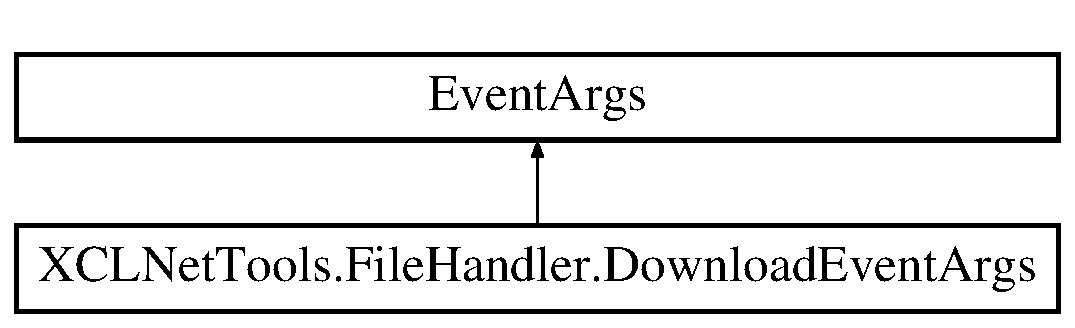
\includegraphics[height=2.000000cm]{class_x_c_l_net_tools_1_1_file_handler_1_1_download_event_args}
\end{center}
\end{figure}
\subsection*{属性}
\begin{DoxyCompactItemize}
\item 
int \hyperlink{class_x_c_l_net_tools_1_1_file_handler_1_1_download_event_args_a1ea772d1ec4b2e0f1f3001fe069bac42}{Bytes\+Received}\hspace{0.3cm}{\ttfamily  \mbox{[}get, set\mbox{]}}
\begin{DoxyCompactList}\small\item\em 已接收的字节数 \end{DoxyCompactList}\item 
int \hyperlink{class_x_c_l_net_tools_1_1_file_handler_1_1_download_event_args_a344cbcca5a213a50ecd25b90340be816}{Total\+Bytes}\hspace{0.3cm}{\ttfamily  \mbox{[}get, set\mbox{]}}
\begin{DoxyCompactList}\small\item\em 总字节数 \end{DoxyCompactList}\item 
byte\mbox{[}$\,$\mbox{]} \hyperlink{class_x_c_l_net_tools_1_1_file_handler_1_1_download_event_args_ae080073b3629650c3befb398e9d7c2e8}{Received\+Data}\hspace{0.3cm}{\ttfamily  \mbox{[}get, set\mbox{]}}
\begin{DoxyCompactList}\small\item\em 当前缓冲区接收的数据 \end{DoxyCompactList}\end{DoxyCompactItemize}


\subsection{详细描述}
下载数据参数 



在文件 Http\+Proc.\+cs 第 50 行定义.



\subsection{属性说明}
\index{X\+C\+L\+Net\+Tools\+::\+File\+Handler\+::\+Download\+Event\+Args@{X\+C\+L\+Net\+Tools\+::\+File\+Handler\+::\+Download\+Event\+Args}!Bytes\+Received@{Bytes\+Received}}
\index{Bytes\+Received@{Bytes\+Received}!X\+C\+L\+Net\+Tools\+::\+File\+Handler\+::\+Download\+Event\+Args@{X\+C\+L\+Net\+Tools\+::\+File\+Handler\+::\+Download\+Event\+Args}}
\subsubsection[{\texorpdfstring{Bytes\+Received}{BytesReceived}}]{\setlength{\rightskip}{0pt plus 5cm}int X\+C\+L\+Net\+Tools.\+File\+Handler.\+Download\+Event\+Args.\+Bytes\+Received\hspace{0.3cm}{\ttfamily [get]}, {\ttfamily [set]}}\hypertarget{class_x_c_l_net_tools_1_1_file_handler_1_1_download_event_args_a1ea772d1ec4b2e0f1f3001fe069bac42}{}\label{class_x_c_l_net_tools_1_1_file_handler_1_1_download_event_args_a1ea772d1ec4b2e0f1f3001fe069bac42}


已接收的字节数 



在文件 Http\+Proc.\+cs 第 60 行定义.

\index{X\+C\+L\+Net\+Tools\+::\+File\+Handler\+::\+Download\+Event\+Args@{X\+C\+L\+Net\+Tools\+::\+File\+Handler\+::\+Download\+Event\+Args}!Received\+Data@{Received\+Data}}
\index{Received\+Data@{Received\+Data}!X\+C\+L\+Net\+Tools\+::\+File\+Handler\+::\+Download\+Event\+Args@{X\+C\+L\+Net\+Tools\+::\+File\+Handler\+::\+Download\+Event\+Args}}
\subsubsection[{\texorpdfstring{Received\+Data}{ReceivedData}}]{\setlength{\rightskip}{0pt plus 5cm}byte \mbox{[}$\,$\mbox{]} X\+C\+L\+Net\+Tools.\+File\+Handler.\+Download\+Event\+Args.\+Received\+Data\hspace{0.3cm}{\ttfamily [get]}, {\ttfamily [set]}}\hypertarget{class_x_c_l_net_tools_1_1_file_handler_1_1_download_event_args_ae080073b3629650c3befb398e9d7c2e8}{}\label{class_x_c_l_net_tools_1_1_file_handler_1_1_download_event_args_ae080073b3629650c3befb398e9d7c2e8}


当前缓冲区接收的数据 



在文件 Http\+Proc.\+cs 第 78 行定义.

\index{X\+C\+L\+Net\+Tools\+::\+File\+Handler\+::\+Download\+Event\+Args@{X\+C\+L\+Net\+Tools\+::\+File\+Handler\+::\+Download\+Event\+Args}!Total\+Bytes@{Total\+Bytes}}
\index{Total\+Bytes@{Total\+Bytes}!X\+C\+L\+Net\+Tools\+::\+File\+Handler\+::\+Download\+Event\+Args@{X\+C\+L\+Net\+Tools\+::\+File\+Handler\+::\+Download\+Event\+Args}}
\subsubsection[{\texorpdfstring{Total\+Bytes}{TotalBytes}}]{\setlength{\rightskip}{0pt plus 5cm}int X\+C\+L\+Net\+Tools.\+File\+Handler.\+Download\+Event\+Args.\+Total\+Bytes\hspace{0.3cm}{\ttfamily [get]}, {\ttfamily [set]}}\hypertarget{class_x_c_l_net_tools_1_1_file_handler_1_1_download_event_args_a344cbcca5a213a50ecd25b90340be816}{}\label{class_x_c_l_net_tools_1_1_file_handler_1_1_download_event_args_a344cbcca5a213a50ecd25b90340be816}


总字节数 



在文件 Http\+Proc.\+cs 第 69 行定义.



该类的文档由以下文件生成\+:\begin{DoxyCompactItemize}
\item 
E\+:/\+Git\+Hub/\+X\+C\+L\+Net\+Tools/\+X\+C\+L\+Net\+Tools/\+File\+Handler/\hyperlink{_http_proc_8cs}{Http\+Proc.\+cs}\end{DoxyCompactItemize}

\hypertarget{class_x_c_l_net_tools_1_1_entity_1_1_enum_1_1_enum_field_model}{\section{X\-C\-L\-Net\-Tools.\-Entity.\-Enum.\-Enum\-Field\-Model类 参考}
\label{class_x_c_l_net_tools_1_1_entity_1_1_enum_1_1_enum_field_model}\index{X\-C\-L\-Net\-Tools.\-Entity.\-Enum.\-Enum\-Field\-Model@{X\-C\-L\-Net\-Tools.\-Entity.\-Enum.\-Enum\-Field\-Model}}
}


Enum项model  


\subsection*{属性}
\begin{DoxyCompactItemize}
\item 
string \hyperlink{class_x_c_l_net_tools_1_1_entity_1_1_enum_1_1_enum_field_model_afba0a6a9289087c382b5d8050ff4dcd0}{Text}\hspace{0.3cm}{\ttfamily  \mbox{[}get, set\mbox{]}}
\begin{DoxyCompactList}\small\item\em text值 \end{DoxyCompactList}\item 
string \hyperlink{class_x_c_l_net_tools_1_1_entity_1_1_enum_1_1_enum_field_model_aa2c519a0507eff410068ee108e7ed845}{Value}\hspace{0.3cm}{\ttfamily  \mbox{[}get, set\mbox{]}}
\begin{DoxyCompactList}\small\item\em value值 \end{DoxyCompactList}\item 
string \hyperlink{class_x_c_l_net_tools_1_1_entity_1_1_enum_1_1_enum_field_model_aac9ea6b895da17a78a261f2721a6da08}{Description}\hspace{0.3cm}{\ttfamily  \mbox{[}get, set\mbox{]}}
\begin{DoxyCompactList}\small\item\em description特性 \end{DoxyCompactList}\end{DoxyCompactItemize}


\subsection{详细描述}
Enum项model 



在文件 Enum\-Field\-Model.\-cs 第 33 行定义.



\subsection{属性说明}
\hypertarget{class_x_c_l_net_tools_1_1_entity_1_1_enum_1_1_enum_field_model_aac9ea6b895da17a78a261f2721a6da08}{\index{X\-C\-L\-Net\-Tools\-::\-Entity\-::\-Enum\-::\-Enum\-Field\-Model@{X\-C\-L\-Net\-Tools\-::\-Entity\-::\-Enum\-::\-Enum\-Field\-Model}!Description@{Description}}
\index{Description@{Description}!XCLNetTools::Entity::Enum::EnumFieldModel@{X\-C\-L\-Net\-Tools\-::\-Entity\-::\-Enum\-::\-Enum\-Field\-Model}}
\subsubsection[{Description}]{\setlength{\rightskip}{0pt plus 5cm}string X\-C\-L\-Net\-Tools.\-Entity.\-Enum.\-Enum\-Field\-Model.\-Description\hspace{0.3cm}{\ttfamily [get]}, {\ttfamily [set]}}}\label{class_x_c_l_net_tools_1_1_entity_1_1_enum_1_1_enum_field_model_aac9ea6b895da17a78a261f2721a6da08}


description特性 



在文件 Enum\-Field\-Model.\-cs 第 48 行定义.

\hypertarget{class_x_c_l_net_tools_1_1_entity_1_1_enum_1_1_enum_field_model_afba0a6a9289087c382b5d8050ff4dcd0}{\index{X\-C\-L\-Net\-Tools\-::\-Entity\-::\-Enum\-::\-Enum\-Field\-Model@{X\-C\-L\-Net\-Tools\-::\-Entity\-::\-Enum\-::\-Enum\-Field\-Model}!Text@{Text}}
\index{Text@{Text}!XCLNetTools::Entity::Enum::EnumFieldModel@{X\-C\-L\-Net\-Tools\-::\-Entity\-::\-Enum\-::\-Enum\-Field\-Model}}
\subsubsection[{Text}]{\setlength{\rightskip}{0pt plus 5cm}string X\-C\-L\-Net\-Tools.\-Entity.\-Enum.\-Enum\-Field\-Model.\-Text\hspace{0.3cm}{\ttfamily [get]}, {\ttfamily [set]}}}\label{class_x_c_l_net_tools_1_1_entity_1_1_enum_1_1_enum_field_model_afba0a6a9289087c382b5d8050ff4dcd0}


text值 



在文件 Enum\-Field\-Model.\-cs 第 38 行定义.

\hypertarget{class_x_c_l_net_tools_1_1_entity_1_1_enum_1_1_enum_field_model_aa2c519a0507eff410068ee108e7ed845}{\index{X\-C\-L\-Net\-Tools\-::\-Entity\-::\-Enum\-::\-Enum\-Field\-Model@{X\-C\-L\-Net\-Tools\-::\-Entity\-::\-Enum\-::\-Enum\-Field\-Model}!Value@{Value}}
\index{Value@{Value}!XCLNetTools::Entity::Enum::EnumFieldModel@{X\-C\-L\-Net\-Tools\-::\-Entity\-::\-Enum\-::\-Enum\-Field\-Model}}
\subsubsection[{Value}]{\setlength{\rightskip}{0pt plus 5cm}string X\-C\-L\-Net\-Tools.\-Entity.\-Enum.\-Enum\-Field\-Model.\-Value\hspace{0.3cm}{\ttfamily [get]}, {\ttfamily [set]}}}\label{class_x_c_l_net_tools_1_1_entity_1_1_enum_1_1_enum_field_model_aa2c519a0507eff410068ee108e7ed845}


value值 



在文件 Enum\-Field\-Model.\-cs 第 43 行定义.



该类的文档由以下文件生成\-:\begin{DoxyCompactItemize}
\item 
D\-:/\-My\-Data/\-My\-Git/\-Git\-Hub/\-X\-C\-L\-Net\-Tools/\-X\-C\-L\-Net\-Tools/\-Entity/\-Enum/\hyperlink{_enum_field_model_8cs}{Enum\-Field\-Model.\-cs}\end{DoxyCompactItemize}

\hypertarget{class_x_c_l_net_tools_1_1_entity_1_1_enum_1_1_enum_field_t_model_3_01_t_01_4}{\section{X\-C\-L\-Net\-Tools.\-Entity.\-Enum.\-Enum\-Field\-T\-Model$<$ T $>$ 模板类 参考}
\label{class_x_c_l_net_tools_1_1_entity_1_1_enum_1_1_enum_field_t_model_3_01_t_01_4}\index{X\-C\-L\-Net\-Tools.\-Entity.\-Enum.\-Enum\-Field\-T\-Model$<$ T $>$@{X\-C\-L\-Net\-Tools.\-Entity.\-Enum.\-Enum\-Field\-T\-Model$<$ T $>$}}
}


枚举model  


\subsection*{属性}
\begin{DoxyCompactItemize}
\item 
string \hyperlink{class_x_c_l_net_tools_1_1_entity_1_1_enum_1_1_enum_field_t_model_3_01_t_01_4_a19570f5fcd9bb314ca1e7e8f3b8f44b1}{Text}\hspace{0.3cm}{\ttfamily  \mbox{[}get, set\mbox{]}}
\begin{DoxyCompactList}\small\item\em text值 \end{DoxyCompactList}\item 
T \hyperlink{class_x_c_l_net_tools_1_1_entity_1_1_enum_1_1_enum_field_t_model_3_01_t_01_4_a0b6e9efa5eb3b809fdc2bbb675a4e8e3}{Value}\hspace{0.3cm}{\ttfamily  \mbox{[}get, set\mbox{]}}
\begin{DoxyCompactList}\small\item\em value值 \end{DoxyCompactList}\item 
string \hyperlink{class_x_c_l_net_tools_1_1_entity_1_1_enum_1_1_enum_field_t_model_3_01_t_01_4_a6702736fc7d4f0f7cfefb74722f9c2ba}{Description}\hspace{0.3cm}{\ttfamily  \mbox{[}get, set\mbox{]}}
\begin{DoxyCompactList}\small\item\em description特性 \end{DoxyCompactList}\end{DoxyCompactItemize}


\subsection{详细描述}
枚举model 


\begin{DoxyTemplParams}{Template Parameters}
{\em T} & 枚举value值类型(可为byte、sbyte、short、ushort、int、uint、long 或 ulong。)\\
\hline
\end{DoxyTemplParams}


在文件 Enum\-Field\-T\-Model.\-cs 第 18 行定义.



\subsection{属性说明}
\hypertarget{class_x_c_l_net_tools_1_1_entity_1_1_enum_1_1_enum_field_t_model_3_01_t_01_4_a6702736fc7d4f0f7cfefb74722f9c2ba}{\index{X\-C\-L\-Net\-Tools\-::\-Entity\-::\-Enum\-::\-Enum\-Field\-T\-Model$<$ T $>$@{X\-C\-L\-Net\-Tools\-::\-Entity\-::\-Enum\-::\-Enum\-Field\-T\-Model$<$ T $>$}!Description@{Description}}
\index{Description@{Description}!XCLNetTools::Entity::Enum::EnumFieldTModel< T >@{X\-C\-L\-Net\-Tools\-::\-Entity\-::\-Enum\-::\-Enum\-Field\-T\-Model$<$ T $>$}}
\subsubsection[{Description}]{\setlength{\rightskip}{0pt plus 5cm}string X\-C\-L\-Net\-Tools.\-Entity.\-Enum.\-Enum\-Field\-T\-Model$<$ T $>$.Description\hspace{0.3cm}{\ttfamily [get]}, {\ttfamily [set]}}}\label{class_x_c_l_net_tools_1_1_entity_1_1_enum_1_1_enum_field_t_model_3_01_t_01_4_a6702736fc7d4f0f7cfefb74722f9c2ba}


description特性 



在文件 Enum\-Field\-T\-Model.\-cs 第 33 行定义.

\hypertarget{class_x_c_l_net_tools_1_1_entity_1_1_enum_1_1_enum_field_t_model_3_01_t_01_4_a19570f5fcd9bb314ca1e7e8f3b8f44b1}{\index{X\-C\-L\-Net\-Tools\-::\-Entity\-::\-Enum\-::\-Enum\-Field\-T\-Model$<$ T $>$@{X\-C\-L\-Net\-Tools\-::\-Entity\-::\-Enum\-::\-Enum\-Field\-T\-Model$<$ T $>$}!Text@{Text}}
\index{Text@{Text}!XCLNetTools::Entity::Enum::EnumFieldTModel< T >@{X\-C\-L\-Net\-Tools\-::\-Entity\-::\-Enum\-::\-Enum\-Field\-T\-Model$<$ T $>$}}
\subsubsection[{Text}]{\setlength{\rightskip}{0pt plus 5cm}string X\-C\-L\-Net\-Tools.\-Entity.\-Enum.\-Enum\-Field\-T\-Model$<$ T $>$.Text\hspace{0.3cm}{\ttfamily [get]}, {\ttfamily [set]}}}\label{class_x_c_l_net_tools_1_1_entity_1_1_enum_1_1_enum_field_t_model_3_01_t_01_4_a19570f5fcd9bb314ca1e7e8f3b8f44b1}


text值 



在文件 Enum\-Field\-T\-Model.\-cs 第 23 行定义.

\hypertarget{class_x_c_l_net_tools_1_1_entity_1_1_enum_1_1_enum_field_t_model_3_01_t_01_4_a0b6e9efa5eb3b809fdc2bbb675a4e8e3}{\index{X\-C\-L\-Net\-Tools\-::\-Entity\-::\-Enum\-::\-Enum\-Field\-T\-Model$<$ T $>$@{X\-C\-L\-Net\-Tools\-::\-Entity\-::\-Enum\-::\-Enum\-Field\-T\-Model$<$ T $>$}!Value@{Value}}
\index{Value@{Value}!XCLNetTools::Entity::Enum::EnumFieldTModel< T >@{X\-C\-L\-Net\-Tools\-::\-Entity\-::\-Enum\-::\-Enum\-Field\-T\-Model$<$ T $>$}}
\subsubsection[{Value}]{\setlength{\rightskip}{0pt plus 5cm}T X\-C\-L\-Net\-Tools.\-Entity.\-Enum.\-Enum\-Field\-T\-Model$<$ T $>$.Value\hspace{0.3cm}{\ttfamily [get]}, {\ttfamily [set]}}}\label{class_x_c_l_net_tools_1_1_entity_1_1_enum_1_1_enum_field_t_model_3_01_t_01_4_a0b6e9efa5eb3b809fdc2bbb675a4e8e3}


value值 



在文件 Enum\-Field\-T\-Model.\-cs 第 28 行定义.



该类的文档由以下文件生成\-:\begin{DoxyCompactItemize}
\item 
D\-:/\-My\-Data/\-My\-Git/\-Git\-Hub/\-X\-C\-L\-Net\-Tools/\-X\-C\-L\-Net\-Tools/\-Entity/\-Enum/\hyperlink{_enum_field_t_model_8cs}{Enum\-Field\-T\-Model.\-cs}\end{DoxyCompactItemize}

\hypertarget{class_x_c_l_net_tools_1_1_enum_1_1_enum_helper}{}\section{X\+C\+L\+Net\+Tools.\+Enum.\+Enum\+Helper类 参考}
\label{class_x_c_l_net_tools_1_1_enum_1_1_enum_helper}\index{X\+C\+L\+Net\+Tools.\+Enum.\+Enum\+Helper@{X\+C\+L\+Net\+Tools.\+Enum.\+Enum\+Helper}}


枚举帮助类  


\subsection*{静态 Public 成员函数}
\begin{DoxyCompactItemize}
\item 
static List$<$ \hyperlink{class_x_c_l_net_tools_1_1_entity_1_1_enum_1_1_enum_field_model}{X\+C\+L\+Net\+Tools.\+Entity.\+Enum.\+Enum\+Field\+Model} $>$ \hyperlink{class_x_c_l_net_tools_1_1_enum_1_1_enum_helper_acdcc3f9200705cc0831c1395f5d2c51e}{Get\+Enum\+Field\+Model\+List} (Type em\+Type)
\begin{DoxyCompactList}\small\item\em 将枚举转为\+List(包含自定义属性description)(value为int型的string) 已按枚举的value升序排列 \end{DoxyCompactList}\item 
static List$<$ \hyperlink{class_x_c_l_net_tools_1_1_entity_1_1_enum_1_1_enum_field_t_model}{X\+C\+L\+Net\+Tools.\+Entity.\+Enum.\+Enum\+Field\+T\+Model}$<$ T $>$ $>$ \hyperlink{class_x_c_l_net_tools_1_1_enum_1_1_enum_helper_a919aa80b589b8038b8db6f731b50556d}{Get\+Enum\+Field\+T\+Model\+List$<$ T $>$} (Type em\+Type)
\begin{DoxyCompactList}\small\item\em 将枚举转为\+List(包含自定义属性description) 已按枚举的value升序排列 \end{DoxyCompactList}\item 
static string \hyperlink{class_x_c_l_net_tools_1_1_enum_1_1_enum_helper_a3445493f9dd4798778af8ecfb2062b1b}{Get\+Enum\+Desc$<$ T $>$} (T enumtype)
\begin{DoxyCompactList}\small\item\em 获取枚举的description注解 \end{DoxyCompactList}\item 
static string \hyperlink{class_x_c_l_net_tools_1_1_enum_1_1_enum_helper_ac1c67f6247644347ed4673965832feaf}{Get\+Enum\+Description\+By\+Text} (Type T, string text)
\begin{DoxyCompactList}\small\item\em 根据枚举text,获取枚举description \end{DoxyCompactList}\item 
static List$<$ \hyperlink{class_x_c_l_net_tools_1_1_entity_1_1_text_value}{X\+C\+L\+Net\+Tools.\+Entity.\+Text\+Value} $>$ \hyperlink{class_x_c_l_net_tools_1_1_enum_1_1_enum_helper_a0f98e6348aacd00a6254794e6565c173}{Get\+List} (Type type)
\begin{DoxyCompactList}\small\item\em 将枚举转为list的形式 \end{DoxyCompactList}\item 
static bool \hyperlink{class_x_c_l_net_tools_1_1_enum_1_1_enum_helper_a364b52512aee90c0f2530745f4127047}{Is\+Exist\+Enum\+Value} (int v, Type type)
\begin{DoxyCompactList}\small\item\em 判断数字是否属于该枚举 \end{DoxyCompactList}\item 
static int \hyperlink{class_x_c_l_net_tools_1_1_enum_1_1_enum_helper_ab5d340064717d8cf3c9c6036d3770b1f}{Get\+Value\+By\+Text} (List$<$ \hyperlink{class_x_c_l_net_tools_1_1_entity_1_1_text_value}{X\+C\+L\+Net\+Tools.\+Entity.\+Text\+Value} $>$ lst, string text)
\begin{DoxyCompactList}\small\item\em 根据名获取值(若未找到,则返回-\/1) \end{DoxyCompactList}\item 
static int \hyperlink{class_x_c_l_net_tools_1_1_enum_1_1_enum_helper_a8ee641787655d2b4f06cb51486ea8be3}{Get\+Bit\+O\+R\+Value$<$ T $>$} (List$<$ T $>$ em)
\begin{DoxyCompactList}\small\item\em 将多个枚举项进行(按位或)操作,返回int型,若失败,则返回null \end{DoxyCompactList}\item 
static List$<$ T $>$ \hyperlink{class_x_c_l_net_tools_1_1_enum_1_1_enum_helper_a7023c3a9e2c46de0cdeed71bce2cfb6a}{Get\+Enum\+List\+By\+Bit\+Value$<$ T $>$} (int val)
\begin{DoxyCompactList}\small\item\em 根据多个枚举项(按位或)之后的int值,返回枚举list \end{DoxyCompactList}\item 
static long \hyperlink{class_x_c_l_net_tools_1_1_enum_1_1_enum_helper_a43bf704153939cd6950d5d88e072c691}{Get\+Enum\+Sum\+Value} (Type em)
\begin{DoxyCompactList}\small\item\em 将指定枚举的值求和 \end{DoxyCompactList}\item 
static long \hyperlink{class_x_c_l_net_tools_1_1_enum_1_1_enum_helper_a8111ec28e6283a2c1964b367b68351c2}{Get\+Min\+Value} (Type em)
\begin{DoxyCompactList}\small\item\em 获取枚举的最小值 \end{DoxyCompactList}\item 
static long \hyperlink{class_x_c_l_net_tools_1_1_enum_1_1_enum_helper_aa7edc75ec210b0c0740978a392e78b32}{Get\+Max\+Value} (Type em)
\begin{DoxyCompactList}\small\item\em 获取枚举的最大值 \end{DoxyCompactList}\item 
static bool \hyperlink{class_x_c_l_net_tools_1_1_enum_1_1_enum_helper_aff77ff22fe3efa1fbac6dd465ea67dc7}{Is\+In\+Range} (Type em, long val)
\begin{DoxyCompactList}\small\item\em 判断指定值是否超出指定枚举的值范围 \end{DoxyCompactList}\end{DoxyCompactItemize}


\subsection{详细描述}
枚举帮助类 



在文件 Enum\+Helper.\+cs 第 20 行定义.



\subsection{成员函数说明}
\index{X\+C\+L\+Net\+Tools\+::\+Enum\+::\+Enum\+Helper@{X\+C\+L\+Net\+Tools\+::\+Enum\+::\+Enum\+Helper}!Get\+Bit\+O\+R\+Value$<$ T $>$@{Get\+Bit\+O\+R\+Value$<$ T $>$}}
\index{Get\+Bit\+O\+R\+Value$<$ T $>$@{Get\+Bit\+O\+R\+Value$<$ T $>$}!X\+C\+L\+Net\+Tools\+::\+Enum\+::\+Enum\+Helper@{X\+C\+L\+Net\+Tools\+::\+Enum\+::\+Enum\+Helper}}
\subsubsection[{\texorpdfstring{Get\+Bit\+O\+R\+Value$<$ T $>$(\+List$<$ T $>$ em)}{GetBitORValue< T >(List< T > em)}}]{\setlength{\rightskip}{0pt plus 5cm}static int X\+C\+L\+Net\+Tools.\+Enum.\+Enum\+Helper.\+Get\+Bit\+O\+R\+Value$<$ T $>$ (
\begin{DoxyParamCaption}
\item[{List$<$ T $>$}]{em}
\end{DoxyParamCaption}
)\hspace{0.3cm}{\ttfamily [static]}}\hypertarget{class_x_c_l_net_tools_1_1_enum_1_1_enum_helper_a8ee641787655d2b4f06cb51486ea8be3}{}\label{class_x_c_l_net_tools_1_1_enum_1_1_enum_helper_a8ee641787655d2b4f06cb51486ea8be3}


将多个枚举项进行(按位或)操作,返回int型,若失败,则返回null 

\begin{DoxyReturn}{返回}
结果值
\end{DoxyReturn}


在文件 Enum\+Helper.\+cs 第 211 行定义.

\index{X\+C\+L\+Net\+Tools\+::\+Enum\+::\+Enum\+Helper@{X\+C\+L\+Net\+Tools\+::\+Enum\+::\+Enum\+Helper}!Get\+Enum\+Desc$<$ T $>$@{Get\+Enum\+Desc$<$ T $>$}}
\index{Get\+Enum\+Desc$<$ T $>$@{Get\+Enum\+Desc$<$ T $>$}!X\+C\+L\+Net\+Tools\+::\+Enum\+::\+Enum\+Helper@{X\+C\+L\+Net\+Tools\+::\+Enum\+::\+Enum\+Helper}}
\subsubsection[{\texorpdfstring{Get\+Enum\+Desc$<$ T $>$(\+T enumtype)}{GetEnumDesc< T >(T enumtype)}}]{\setlength{\rightskip}{0pt plus 5cm}static string X\+C\+L\+Net\+Tools.\+Enum.\+Enum\+Helper.\+Get\+Enum\+Desc$<$ T $>$ (
\begin{DoxyParamCaption}
\item[{T}]{enumtype}
\end{DoxyParamCaption}
)\hspace{0.3cm}{\ttfamily [static]}}\hypertarget{class_x_c_l_net_tools_1_1_enum_1_1_enum_helper_a3445493f9dd4798778af8ecfb2062b1b}{}\label{class_x_c_l_net_tools_1_1_enum_1_1_enum_helper_a3445493f9dd4798778af8ecfb2062b1b}


获取枚举的description注解 

\begin{DoxyReturn}{返回}
枚举的描述
\end{DoxyReturn}


在文件 Enum\+Helper.\+cs 第 94 行定义.

\index{X\+C\+L\+Net\+Tools\+::\+Enum\+::\+Enum\+Helper@{X\+C\+L\+Net\+Tools\+::\+Enum\+::\+Enum\+Helper}!Get\+Enum\+Description\+By\+Text@{Get\+Enum\+Description\+By\+Text}}
\index{Get\+Enum\+Description\+By\+Text@{Get\+Enum\+Description\+By\+Text}!X\+C\+L\+Net\+Tools\+::\+Enum\+::\+Enum\+Helper@{X\+C\+L\+Net\+Tools\+::\+Enum\+::\+Enum\+Helper}}
\subsubsection[{\texorpdfstring{Get\+Enum\+Description\+By\+Text(\+Type T, string text)}{GetEnumDescriptionByText(Type T, string text)}}]{\setlength{\rightskip}{0pt plus 5cm}static string X\+C\+L\+Net\+Tools.\+Enum.\+Enum\+Helper.\+Get\+Enum\+Description\+By\+Text (
\begin{DoxyParamCaption}
\item[{Type}]{T, }
\item[{string}]{text}
\end{DoxyParamCaption}
)\hspace{0.3cm}{\ttfamily [static]}}\hypertarget{class_x_c_l_net_tools_1_1_enum_1_1_enum_helper_ac1c67f6247644347ed4673965832feaf}{}\label{class_x_c_l_net_tools_1_1_enum_1_1_enum_helper_ac1c67f6247644347ed4673965832feaf}


根据枚举text,获取枚举description 

\begin{DoxyReturn}{返回}
枚举的描述
\end{DoxyReturn}


在文件 Enum\+Helper.\+cs 第 121 行定义.

\index{X\+C\+L\+Net\+Tools\+::\+Enum\+::\+Enum\+Helper@{X\+C\+L\+Net\+Tools\+::\+Enum\+::\+Enum\+Helper}!Get\+Enum\+Field\+Model\+List@{Get\+Enum\+Field\+Model\+List}}
\index{Get\+Enum\+Field\+Model\+List@{Get\+Enum\+Field\+Model\+List}!X\+C\+L\+Net\+Tools\+::\+Enum\+::\+Enum\+Helper@{X\+C\+L\+Net\+Tools\+::\+Enum\+::\+Enum\+Helper}}
\subsubsection[{\texorpdfstring{Get\+Enum\+Field\+Model\+List(\+Type em\+Type)}{GetEnumFieldModelList(Type emType)}}]{\setlength{\rightskip}{0pt plus 5cm}static List$<${\bf X\+C\+L\+Net\+Tools.\+Entity.\+Enum.\+Enum\+Field\+Model}$>$ X\+C\+L\+Net\+Tools.\+Enum.\+Enum\+Helper.\+Get\+Enum\+Field\+Model\+List (
\begin{DoxyParamCaption}
\item[{Type}]{em\+Type}
\end{DoxyParamCaption}
)\hspace{0.3cm}{\ttfamily [static]}}\hypertarget{class_x_c_l_net_tools_1_1_enum_1_1_enum_helper_acdcc3f9200705cc0831c1395f5d2c51e}{}\label{class_x_c_l_net_tools_1_1_enum_1_1_enum_helper_acdcc3f9200705cc0831c1395f5d2c51e}


将枚举转为\+List(包含自定义属性description)(value为int型的string) 已按枚举的value升序排列 


\begin{DoxyParams}{参数}
{\em em\+Type} & 枚举type\\
\hline
\end{DoxyParams}
\begin{DoxyReturn}{返回}
枚举的\+List
\end{DoxyReturn}


在文件 Enum\+Helper.\+cs 第 28 行定义.

\index{X\+C\+L\+Net\+Tools\+::\+Enum\+::\+Enum\+Helper@{X\+C\+L\+Net\+Tools\+::\+Enum\+::\+Enum\+Helper}!Get\+Enum\+Field\+T\+Model\+List$<$ T $>$@{Get\+Enum\+Field\+T\+Model\+List$<$ T $>$}}
\index{Get\+Enum\+Field\+T\+Model\+List$<$ T $>$@{Get\+Enum\+Field\+T\+Model\+List$<$ T $>$}!X\+C\+L\+Net\+Tools\+::\+Enum\+::\+Enum\+Helper@{X\+C\+L\+Net\+Tools\+::\+Enum\+::\+Enum\+Helper}}
\subsubsection[{\texorpdfstring{Get\+Enum\+Field\+T\+Model\+List$<$ T $>$(\+Type em\+Type)}{GetEnumFieldTModelList< T >(Type emType)}}]{\setlength{\rightskip}{0pt plus 5cm}static List$<${\bf X\+C\+L\+Net\+Tools.\+Entity.\+Enum.\+Enum\+Field\+T\+Model}$<$T$>$ $>$ X\+C\+L\+Net\+Tools.\+Enum.\+Enum\+Helper.\+Get\+Enum\+Field\+T\+Model\+List$<$ T $>$ (
\begin{DoxyParamCaption}
\item[{Type}]{em\+Type}
\end{DoxyParamCaption}
)\hspace{0.3cm}{\ttfamily [static]}}\hypertarget{class_x_c_l_net_tools_1_1_enum_1_1_enum_helper_a919aa80b589b8038b8db6f731b50556d}{}\label{class_x_c_l_net_tools_1_1_enum_1_1_enum_helper_a919aa80b589b8038b8db6f731b50556d}


将枚举转为\+List(包含自定义属性description) 已按枚举的value升序排列 


\begin{DoxyParams}{参数}
{\em em\+Type} & 枚举type\\
\hline
\end{DoxyParams}

\begin{DoxyTemplParams}{Template Parameters}
{\em T} & 枚举value的类型((可为byte、sbyte、short、ushort、int、uint、long 或 ulong。))\\
\hline
\end{DoxyTemplParams}
\begin{DoxyReturn}{返回}
枚举的\+List
\end{DoxyReturn}


在文件 Enum\+Helper.\+cs 第 55 行定义.

\index{X\+C\+L\+Net\+Tools\+::\+Enum\+::\+Enum\+Helper@{X\+C\+L\+Net\+Tools\+::\+Enum\+::\+Enum\+Helper}!Get\+Enum\+List\+By\+Bit\+Value$<$ T $>$@{Get\+Enum\+List\+By\+Bit\+Value$<$ T $>$}}
\index{Get\+Enum\+List\+By\+Bit\+Value$<$ T $>$@{Get\+Enum\+List\+By\+Bit\+Value$<$ T $>$}!X\+C\+L\+Net\+Tools\+::\+Enum\+::\+Enum\+Helper@{X\+C\+L\+Net\+Tools\+::\+Enum\+::\+Enum\+Helper}}
\subsubsection[{\texorpdfstring{Get\+Enum\+List\+By\+Bit\+Value$<$ T $>$(int val)}{GetEnumListByBitValue< T >(int val)}}]{\setlength{\rightskip}{0pt plus 5cm}static List$<$T$>$ X\+C\+L\+Net\+Tools.\+Enum.\+Enum\+Helper.\+Get\+Enum\+List\+By\+Bit\+Value$<$ T $>$ (
\begin{DoxyParamCaption}
\item[{int}]{val}
\end{DoxyParamCaption}
)\hspace{0.3cm}{\ttfamily [static]}}\hypertarget{class_x_c_l_net_tools_1_1_enum_1_1_enum_helper_a7023c3a9e2c46de0cdeed71bce2cfb6a}{}\label{class_x_c_l_net_tools_1_1_enum_1_1_enum_helper_a7023c3a9e2c46de0cdeed71bce2cfb6a}


根据多个枚举项(按位或)之后的int值,返回枚举list 

\begin{DoxyReturn}{返回}
枚举list
\end{DoxyReturn}


在文件 Enum\+Helper.\+cs 第 233 行定义.

\index{X\+C\+L\+Net\+Tools\+::\+Enum\+::\+Enum\+Helper@{X\+C\+L\+Net\+Tools\+::\+Enum\+::\+Enum\+Helper}!Get\+Enum\+Sum\+Value@{Get\+Enum\+Sum\+Value}}
\index{Get\+Enum\+Sum\+Value@{Get\+Enum\+Sum\+Value}!X\+C\+L\+Net\+Tools\+::\+Enum\+::\+Enum\+Helper@{X\+C\+L\+Net\+Tools\+::\+Enum\+::\+Enum\+Helper}}
\subsubsection[{\texorpdfstring{Get\+Enum\+Sum\+Value(\+Type em)}{GetEnumSumValue(Type em)}}]{\setlength{\rightskip}{0pt plus 5cm}static long X\+C\+L\+Net\+Tools.\+Enum.\+Enum\+Helper.\+Get\+Enum\+Sum\+Value (
\begin{DoxyParamCaption}
\item[{Type}]{em}
\end{DoxyParamCaption}
)\hspace{0.3cm}{\ttfamily [static]}}\hypertarget{class_x_c_l_net_tools_1_1_enum_1_1_enum_helper_a43bf704153939cd6950d5d88e072c691}{}\label{class_x_c_l_net_tools_1_1_enum_1_1_enum_helper_a43bf704153939cd6950d5d88e072c691}


将指定枚举的值求和 

\begin{DoxyReturn}{返回}
求和后的结果值
\end{DoxyReturn}


在文件 Enum\+Helper.\+cs 第 259 行定义.

\index{X\+C\+L\+Net\+Tools\+::\+Enum\+::\+Enum\+Helper@{X\+C\+L\+Net\+Tools\+::\+Enum\+::\+Enum\+Helper}!Get\+List@{Get\+List}}
\index{Get\+List@{Get\+List}!X\+C\+L\+Net\+Tools\+::\+Enum\+::\+Enum\+Helper@{X\+C\+L\+Net\+Tools\+::\+Enum\+::\+Enum\+Helper}}
\subsubsection[{\texorpdfstring{Get\+List(\+Type type)}{GetList(Type type)}}]{\setlength{\rightskip}{0pt plus 5cm}static List$<${\bf X\+C\+L\+Net\+Tools.\+Entity.\+Text\+Value}$>$ X\+C\+L\+Net\+Tools.\+Enum.\+Enum\+Helper.\+Get\+List (
\begin{DoxyParamCaption}
\item[{Type}]{type}
\end{DoxyParamCaption}
)\hspace{0.3cm}{\ttfamily [static]}}\hypertarget{class_x_c_l_net_tools_1_1_enum_1_1_enum_helper_a0f98e6348aacd00a6254794e6565c173}{}\label{class_x_c_l_net_tools_1_1_enum_1_1_enum_helper_a0f98e6348aacd00a6254794e6565c173}


将枚举转为list的形式 


\begin{DoxyParams}{参数}
{\em type} & 枚举的typeof\\
\hline
\end{DoxyParams}
\begin{DoxyReturn}{返回}
枚举的list形式
\end{DoxyReturn}


在文件 Enum\+Helper.\+cs 第 145 行定义.

\index{X\+C\+L\+Net\+Tools\+::\+Enum\+::\+Enum\+Helper@{X\+C\+L\+Net\+Tools\+::\+Enum\+::\+Enum\+Helper}!Get\+Max\+Value@{Get\+Max\+Value}}
\index{Get\+Max\+Value@{Get\+Max\+Value}!X\+C\+L\+Net\+Tools\+::\+Enum\+::\+Enum\+Helper@{X\+C\+L\+Net\+Tools\+::\+Enum\+::\+Enum\+Helper}}
\subsubsection[{\texorpdfstring{Get\+Max\+Value(\+Type em)}{GetMaxValue(Type em)}}]{\setlength{\rightskip}{0pt plus 5cm}static long X\+C\+L\+Net\+Tools.\+Enum.\+Enum\+Helper.\+Get\+Max\+Value (
\begin{DoxyParamCaption}
\item[{Type}]{em}
\end{DoxyParamCaption}
)\hspace{0.3cm}{\ttfamily [static]}}\hypertarget{class_x_c_l_net_tools_1_1_enum_1_1_enum_helper_aa7edc75ec210b0c0740978a392e78b32}{}\label{class_x_c_l_net_tools_1_1_enum_1_1_enum_helper_aa7edc75ec210b0c0740978a392e78b32}


获取枚举的最大值 


\begin{DoxyParams}{参数}
{\em em} & 指定枚举\\
\hline
\end{DoxyParams}
\begin{DoxyReturn}{返回}
枚举项中的最大值
\end{DoxyReturn}


在文件 Enum\+Helper.\+cs 第 289 行定义.

\index{X\+C\+L\+Net\+Tools\+::\+Enum\+::\+Enum\+Helper@{X\+C\+L\+Net\+Tools\+::\+Enum\+::\+Enum\+Helper}!Get\+Min\+Value@{Get\+Min\+Value}}
\index{Get\+Min\+Value@{Get\+Min\+Value}!X\+C\+L\+Net\+Tools\+::\+Enum\+::\+Enum\+Helper@{X\+C\+L\+Net\+Tools\+::\+Enum\+::\+Enum\+Helper}}
\subsubsection[{\texorpdfstring{Get\+Min\+Value(\+Type em)}{GetMinValue(Type em)}}]{\setlength{\rightskip}{0pt plus 5cm}static long X\+C\+L\+Net\+Tools.\+Enum.\+Enum\+Helper.\+Get\+Min\+Value (
\begin{DoxyParamCaption}
\item[{Type}]{em}
\end{DoxyParamCaption}
)\hspace{0.3cm}{\ttfamily [static]}}\hypertarget{class_x_c_l_net_tools_1_1_enum_1_1_enum_helper_a8111ec28e6283a2c1964b367b68351c2}{}\label{class_x_c_l_net_tools_1_1_enum_1_1_enum_helper_a8111ec28e6283a2c1964b367b68351c2}


获取枚举的最小值 


\begin{DoxyParams}{参数}
{\em em} & 指定枚举\\
\hline
\end{DoxyParams}
\begin{DoxyReturn}{返回}
枚举项中的最小值
\end{DoxyReturn}


在文件 Enum\+Helper.\+cs 第 274 行定义.

\index{X\+C\+L\+Net\+Tools\+::\+Enum\+::\+Enum\+Helper@{X\+C\+L\+Net\+Tools\+::\+Enum\+::\+Enum\+Helper}!Get\+Value\+By\+Text@{Get\+Value\+By\+Text}}
\index{Get\+Value\+By\+Text@{Get\+Value\+By\+Text}!X\+C\+L\+Net\+Tools\+::\+Enum\+::\+Enum\+Helper@{X\+C\+L\+Net\+Tools\+::\+Enum\+::\+Enum\+Helper}}
\subsubsection[{\texorpdfstring{Get\+Value\+By\+Text(\+List$<$ X\+C\+L\+Net\+Tools.\+Entity.\+Text\+Value $>$ lst, string text)}{GetValueByText(List< XCLNetTools.Entity.TextValue > lst, string text)}}]{\setlength{\rightskip}{0pt plus 5cm}static int X\+C\+L\+Net\+Tools.\+Enum.\+Enum\+Helper.\+Get\+Value\+By\+Text (
\begin{DoxyParamCaption}
\item[{List$<$ {\bf X\+C\+L\+Net\+Tools.\+Entity.\+Text\+Value} $>$}]{lst, }
\item[{string}]{text}
\end{DoxyParamCaption}
)\hspace{0.3cm}{\ttfamily [static]}}\hypertarget{class_x_c_l_net_tools_1_1_enum_1_1_enum_helper_ab5d340064717d8cf3c9c6036d3770b1f}{}\label{class_x_c_l_net_tools_1_1_enum_1_1_enum_helper_ab5d340064717d8cf3c9c6036d3770b1f}


根据名获取值(若未找到,则返回-\/1) 


\begin{DoxyParams}{参数}
{\em lst} & 枚举的list形式\\
\hline
{\em text} & 枚举项的名称\\
\hline
\end{DoxyParams}
\begin{DoxyReturn}{返回}
该枚举的值
\end{DoxyReturn}


在文件 Enum\+Helper.\+cs 第 193 行定义.

\index{X\+C\+L\+Net\+Tools\+::\+Enum\+::\+Enum\+Helper@{X\+C\+L\+Net\+Tools\+::\+Enum\+::\+Enum\+Helper}!Is\+Exist\+Enum\+Value@{Is\+Exist\+Enum\+Value}}
\index{Is\+Exist\+Enum\+Value@{Is\+Exist\+Enum\+Value}!X\+C\+L\+Net\+Tools\+::\+Enum\+::\+Enum\+Helper@{X\+C\+L\+Net\+Tools\+::\+Enum\+::\+Enum\+Helper}}
\subsubsection[{\texorpdfstring{Is\+Exist\+Enum\+Value(int v, Type type)}{IsExistEnumValue(int v, Type type)}}]{\setlength{\rightskip}{0pt plus 5cm}static bool X\+C\+L\+Net\+Tools.\+Enum.\+Enum\+Helper.\+Is\+Exist\+Enum\+Value (
\begin{DoxyParamCaption}
\item[{int}]{v, }
\item[{Type}]{type}
\end{DoxyParamCaption}
)\hspace{0.3cm}{\ttfamily [static]}}\hypertarget{class_x_c_l_net_tools_1_1_enum_1_1_enum_helper_a364b52512aee90c0f2530745f4127047}{}\label{class_x_c_l_net_tools_1_1_enum_1_1_enum_helper_a364b52512aee90c0f2530745f4127047}


判断数字是否属于该枚举 


\begin{DoxyParams}{参数}
{\em v} & 枚举的value,就是数字\\
\hline
{\em type} & 枚举的typeof\\
\hline
\end{DoxyParams}
\begin{DoxyReturn}{返回}
true\+:v属于该枚举,反之则不属于
\end{DoxyReturn}


在文件 Enum\+Helper.\+cs 第 172 行定义.

\index{X\+C\+L\+Net\+Tools\+::\+Enum\+::\+Enum\+Helper@{X\+C\+L\+Net\+Tools\+::\+Enum\+::\+Enum\+Helper}!Is\+In\+Range@{Is\+In\+Range}}
\index{Is\+In\+Range@{Is\+In\+Range}!X\+C\+L\+Net\+Tools\+::\+Enum\+::\+Enum\+Helper@{X\+C\+L\+Net\+Tools\+::\+Enum\+::\+Enum\+Helper}}
\subsubsection[{\texorpdfstring{Is\+In\+Range(\+Type em, long val)}{IsInRange(Type em, long val)}}]{\setlength{\rightskip}{0pt plus 5cm}static bool X\+C\+L\+Net\+Tools.\+Enum.\+Enum\+Helper.\+Is\+In\+Range (
\begin{DoxyParamCaption}
\item[{Type}]{em, }
\item[{long}]{val}
\end{DoxyParamCaption}
)\hspace{0.3cm}{\ttfamily [static]}}\hypertarget{class_x_c_l_net_tools_1_1_enum_1_1_enum_helper_aff77ff22fe3efa1fbac6dd465ea67dc7}{}\label{class_x_c_l_net_tools_1_1_enum_1_1_enum_helper_aff77ff22fe3efa1fbac6dd465ea67dc7}


判断指定值是否超出指定枚举的值范围 


\begin{DoxyParams}{参数}
{\em em} & 枚举\\
\hline
{\em val} & 要判断的值\\
\hline
\end{DoxyParams}
\begin{DoxyReturn}{返回}
true:在范围内;false:已超出范围
\end{DoxyReturn}


在文件 Enum\+Helper.\+cs 第 305 行定义.



该类的文档由以下文件生成\+:\begin{DoxyCompactItemize}
\item 
E\+:/\+Git\+Hub/\+X\+C\+L\+Net\+Tools/\+X\+C\+L\+Net\+Tools/\+Enum/\hyperlink{_enum_helper_8cs}{Enum\+Helper.\+cs}\end{DoxyCompactItemize}

\hypertarget{class_x_c_l_net_tools_1_1_message_1_1_error_1_1_error_http_module}{\section{X\-C\-L\-Net\-Tools.\-Message.\-Error.\-Error\-Http\-Module类 参考}
\label{class_x_c_l_net_tools_1_1_message_1_1_error_1_1_error_http_module}\index{X\-C\-L\-Net\-Tools.\-Message.\-Error.\-Error\-Http\-Module@{X\-C\-L\-Net\-Tools.\-Message.\-Error.\-Error\-Http\-Module}}
}


异常处理  


类 X\-C\-L\-Net\-Tools.\-Message.\-Error.\-Error\-Http\-Module 继承关系图\-:\begin{figure}[H]
\begin{center}
\leavevmode
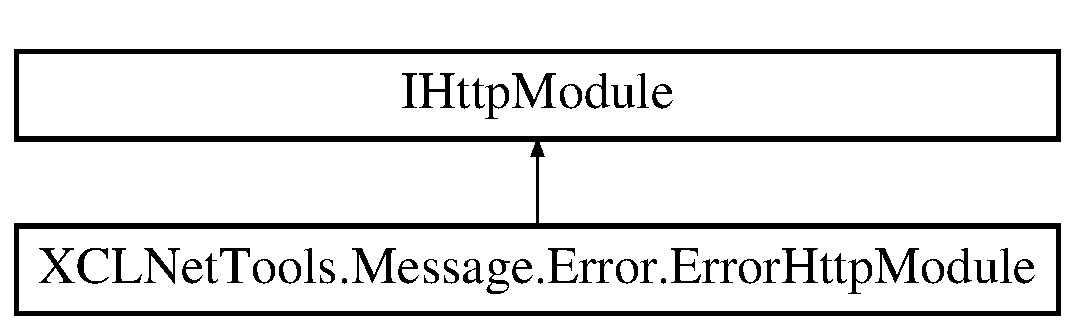
\includegraphics[height=2.000000cm]{class_x_c_l_net_tools_1_1_message_1_1_error_1_1_error_http_module}
\end{center}
\end{figure}
\subsection*{Public 成员函数}
\begin{DoxyCompactItemize}
\item 
void \hyperlink{class_x_c_l_net_tools_1_1_message_1_1_error_1_1_error_http_module_aa4e06d53382795826ed453b62afa265d}{Init} (Http\-Application context)
\begin{DoxyCompactList}\small\item\em 初始化 \end{DoxyCompactList}\item 
void \hyperlink{class_x_c_l_net_tools_1_1_message_1_1_error_1_1_error_http_module_a796d6d747b8620b5e260858e05abd09f}{Dispose} ()
\begin{DoxyCompactList}\small\item\em Dispose \end{DoxyCompactList}\end{DoxyCompactItemize}


\subsection{详细描述}
异常处理 



在文件 Error\-Http\-Module.\-cs 第 18 行定义.



\subsection{成员函数说明}
\hypertarget{class_x_c_l_net_tools_1_1_message_1_1_error_1_1_error_http_module_a796d6d747b8620b5e260858e05abd09f}{\index{X\-C\-L\-Net\-Tools\-::\-Message\-::\-Error\-::\-Error\-Http\-Module@{X\-C\-L\-Net\-Tools\-::\-Message\-::\-Error\-::\-Error\-Http\-Module}!Dispose@{Dispose}}
\index{Dispose@{Dispose}!XCLNetTools::Message::Error::ErrorHttpModule@{X\-C\-L\-Net\-Tools\-::\-Message\-::\-Error\-::\-Error\-Http\-Module}}
\subsubsection[{Dispose}]{\setlength{\rightskip}{0pt plus 5cm}void X\-C\-L\-Net\-Tools.\-Message.\-Error.\-Error\-Http\-Module.\-Dispose (
\begin{DoxyParamCaption}
{}
\end{DoxyParamCaption}
)}}\label{class_x_c_l_net_tools_1_1_message_1_1_error_1_1_error_http_module_a796d6d747b8620b5e260858e05abd09f}


Dispose 



在文件 Error\-Http\-Module.\-cs 第 78 行定义.

\hypertarget{class_x_c_l_net_tools_1_1_message_1_1_error_1_1_error_http_module_aa4e06d53382795826ed453b62afa265d}{\index{X\-C\-L\-Net\-Tools\-::\-Message\-::\-Error\-::\-Error\-Http\-Module@{X\-C\-L\-Net\-Tools\-::\-Message\-::\-Error\-::\-Error\-Http\-Module}!Init@{Init}}
\index{Init@{Init}!XCLNetTools::Message::Error::ErrorHttpModule@{X\-C\-L\-Net\-Tools\-::\-Message\-::\-Error\-::\-Error\-Http\-Module}}
\subsubsection[{Init}]{\setlength{\rightskip}{0pt plus 5cm}void X\-C\-L\-Net\-Tools.\-Message.\-Error.\-Error\-Http\-Module.\-Init (
\begin{DoxyParamCaption}
\item[{Http\-Application}]{context}
\end{DoxyParamCaption}
)}}\label{class_x_c_l_net_tools_1_1_message_1_1_error_1_1_error_http_module_aa4e06d53382795826ed453b62afa265d}


初始化 



在文件 Error\-Http\-Module.\-cs 第 25 行定义.



该类的文档由以下文件生成\-:\begin{DoxyCompactItemize}
\item 
D\-:/\-My\-Data/\-My\-Git/\-Git\-Hub/\-X\-C\-L\-Net\-Tools/\-X\-C\-L\-Net\-Tools/\-Message/\-Error/\hyperlink{_error_http_module_8cs}{Error\-Http\-Module.\-cs}\end{DoxyCompactItemize}

\hypertarget{class_x_c_l_net_tools_1_1_data_handler_1_1_excel_helper}{\section{X\-C\-L\-Net\-Tools.\-Data\-Handler.\-Excel\-Helper类 参考}
\label{class_x_c_l_net_tools_1_1_data_handler_1_1_excel_helper}\index{X\-C\-L\-Net\-Tools.\-Data\-Handler.\-Excel\-Helper@{X\-C\-L\-Net\-Tools.\-Data\-Handler.\-Excel\-Helper}}
}


旧版的excel操作(基于excel.\-dll),建议不要使用此类(用aspose.\-cells)  


\subsection*{Public 成员函数}
\begin{DoxyCompactItemize}
\item 
\hyperlink{class_x_c_l_net_tools_1_1_data_handler_1_1_excel_helper_acebffd827fa8842be172440be3e1a134}{Excel\-Helper} (string templet\-File\-Path, string output\-File\-Path)
\begin{DoxyCompactList}\small\item\em 构造函数,将一个已有\-Excel工作簿作为模板,并指定输出路径 \end{DoxyCompactList}\item 
\hyperlink{class_x_c_l_net_tools_1_1_data_handler_1_1_excel_helper_a7b0a4d5a5f8509b97ed054db15ef23d2}{Excel\-Helper} (string file\-Name)
\begin{DoxyCompactList}\small\item\em 构造函数,打开一个已有的工作簿 \end{DoxyCompactList}\item 
\hyperlink{class_x_c_l_net_tools_1_1_data_handler_1_1_excel_helper_a2a3ce10ddfb59e2560a8faa05abc9976}{Excel\-Helper} ()
\begin{DoxyCompactList}\small\item\em 构造函数,新建一个工作簿 \end{DoxyCompactList}\item 
void \hyperlink{class_x_c_l_net_tools_1_1_data_handler_1_1_excel_helper_aee0dd3e95ba5e89b2043cb7d1c969a1c}{Data\-Table\-To\-Excel} (Data\-Table dt, int rows, int top, int left)
\begin{DoxyCompactList}\small\item\em 将\-Data\-Table数据写入\-Excel文件(自动分页) \end{DoxyCompactList}\item 
void \hyperlink{class_x_c_l_net_tools_1_1_data_handler_1_1_excel_helper_a5a62b1a5ff7569e2236ad5eb7a4efcb8}{Data\-Table\-To\-Excel} (Data\-Table dt, int top, int left)
\begin{DoxyCompactList}\small\item\em 将\-Data\-Table数据写入\-Excel文件(不分页) \end{DoxyCompactList}\item 
void \hyperlink{class_x_c_l_net_tools_1_1_data_handler_1_1_excel_helper_a28b1238b8e1008cb4a39ed189df0b73f}{Data\-Table\-To\-Excel} (Data\-Table dt, int rows, int top, int left, int merge\-Column\-Index)
\begin{DoxyCompactList}\small\item\em 将\-Data\-Table数据写入\-Excel文件(自动分页,并指定要合并的列索引) \end{DoxyCompactList}\item 
void \hyperlink{class_x_c_l_net_tools_1_1_data_handler_1_1_excel_helper_a9f6650dba490907278b2ec278f0ecf5d}{Array\-To\-Excel} (string\mbox{[},\mbox{]} arr, int rows, int top, int left)
\begin{DoxyCompactList}\small\item\em 将二维数组数据写入\-Excel文件(自动分页) \end{DoxyCompactList}\item 
void \hyperlink{class_x_c_l_net_tools_1_1_data_handler_1_1_excel_helper_a5be4d665a31a9347e2fe8b3b58b137af}{Array\-To\-Excel} (string\mbox{[},\mbox{]} arr, int top, int left)
\begin{DoxyCompactList}\small\item\em 将二维数组数据写入\-Excel文件(不分页) \end{DoxyCompactList}\item 
void \hyperlink{class_x_c_l_net_tools_1_1_data_handler_1_1_excel_helper_ad2526a27bf44d46c44d8adb56c868c60}{Array\-To\-Excel} (string\mbox{[},\mbox{]} arr, int top, int left, bool is\-Formula)
\begin{DoxyCompactList}\small\item\em 将二维数组数据写入\-Excel文件(不分页) \end{DoxyCompactList}\item 
void \hyperlink{class_x_c_l_net_tools_1_1_data_handler_1_1_excel_helper_a153dfbee4fd21b4ae6eaa1b75955e849}{Array\-To\-Excel} (string\mbox{[},\mbox{]} arr, int top, int left, bool is\-Formula, int merge\-Column\-Index)
\begin{DoxyCompactList}\small\item\em 将二维数组数据写入\-Excel文件(不分页),合并指定列的相同行 \end{DoxyCompactList}\item 
void \hyperlink{class_x_c_l_net_tools_1_1_data_handler_1_1_excel_helper_a7f91871b4a54529f34b3b95fd0c9f0e9}{Array\-To\-Excel} (int sheet\-Index, string\mbox{[},\mbox{]} arr, int top, int left)
\begin{DoxyCompactList}\small\item\em 将二维数组数据写入\-Excel文件(不分页) \end{DoxyCompactList}\item 
void \hyperlink{class_x_c_l_net_tools_1_1_data_handler_1_1_excel_helper_a24dc63cd234dd2bc58a5833b4dcdcc6e}{Array\-To\-Excel} (string\mbox{[},\mbox{]} arr, int rows, int top, int left, int merge\-Column\-Index)
\begin{DoxyCompactList}\small\item\em 将二维数组数据写入\-Excel文件(自动分页,并指定要合并的列索引) \end{DoxyCompactList}\item 
void \hyperlink{class_x_c_l_net_tools_1_1_data_handler_1_1_excel_helper_a5685e97d3cfd67203faeee2bcdd6c788}{Change\-Current\-Work\-Sheet} (int sheet\-Index)
\begin{DoxyCompactList}\small\item\em 改变当前工作表 \end{DoxyCompactList}\item 
void \hyperlink{class_x_c_l_net_tools_1_1_data_handler_1_1_excel_helper_a417d5331a647da31429ff028821e4012}{Hidden\-Work\-Sheet} (string sheet\-Name)
\begin{DoxyCompactList}\small\item\em 隐藏指定名称的工作表 \end{DoxyCompactList}\item 
void \hyperlink{class_x_c_l_net_tools_1_1_data_handler_1_1_excel_helper_a2b65f3492d6d7eeadd2366db1d1cc992}{Hidden\-Work\-Sheet} (int sheet\-Index)
\begin{DoxyCompactList}\small\item\em 隐藏指定索引的工作表 \end{DoxyCompactList}\item 
void \hyperlink{class_x_c_l_net_tools_1_1_data_handler_1_1_excel_helper_a3aa2c1a6e359f9fe7bba76d803ecbb81}{Copy\-Work\-Sheets} (string sheet\-Name, int sheet\-Count)
\begin{DoxyCompactList}\small\item\em 在指定名称的工作表后面拷贝指定个数的该工作表的副本,并重命名 \end{DoxyCompactList}\item 
void \hyperlink{class_x_c_l_net_tools_1_1_data_handler_1_1_excel_helper_a8947f0bbcbbd82566e9083fd30965862}{Copy\-Work\-Sheet} (int src\-Sheet\-Index, int aim\-Sheet\-Index, string new\-Sheet\-Name)
\begin{DoxyCompactList}\small\item\em 将一个工作表拷贝到另一个工作表后面,并重命名 \end{DoxyCompactList}\item 
void \hyperlink{class_x_c_l_net_tools_1_1_data_handler_1_1_excel_helper_ab6b232c0411cec6a15affbe3664a8cd0}{Delete\-Work\-Sheet} (string sheet\-Name)
\begin{DoxyCompactList}\small\item\em 根据名称删除工作表 \end{DoxyCompactList}\item 
void \hyperlink{class_x_c_l_net_tools_1_1_data_handler_1_1_excel_helper_a21db1bb567b78dce9d069f33b22f4b25}{Delete\-Work\-Sheet} (int sheet\-Index)
\begin{DoxyCompactList}\small\item\em 根据索引删除工作表 \end{DoxyCompactList}\item 
void \hyperlink{class_x_c_l_net_tools_1_1_data_handler_1_1_excel_helper_ab8f108b5bd5c60144bc5666884c5191b}{Set\-Text\-Box} (string textbox\-Name, string text)
\begin{DoxyCompactList}\small\item\em 向指定文本框写入数据,对每个\-Work\-Sheet操作 \end{DoxyCompactList}\item 
void \hyperlink{class_x_c_l_net_tools_1_1_data_handler_1_1_excel_helper_a86d566cea97a41b04cad4c896051b6d9}{Set\-Text\-Box} (int sheet\-Index, string textbox\-Name, string text)
\begin{DoxyCompactList}\small\item\em 向指定文本框写入数据,对指定\-Work\-Sheet操作 \end{DoxyCompactList}\item 
void \hyperlink{class_x_c_l_net_tools_1_1_data_handler_1_1_excel_helper_ab9019cd73148e6176ed400ba305d15e5}{Set\-Text\-Boxes} (Hashtable ht)
\begin{DoxyCompactList}\small\item\em 向文本框写入数据,对每个\-Work\-Sheet操作 \end{DoxyCompactList}\item 
void \hyperlink{class_x_c_l_net_tools_1_1_data_handler_1_1_excel_helper_a2b06a36aeacbea3f7158bb45db1f59a2}{Set\-Text\-Boxes} (int sheet\-Index, Hashtable ht)
\begin{DoxyCompactList}\small\item\em 向文本框写入数据,对指定\-Work\-Sheet操作 \end{DoxyCompactList}\item 
void \hyperlink{class_x_c_l_net_tools_1_1_data_handler_1_1_excel_helper_a1210a9f840d18b18bec230c71eb00564}{Set\-Cells} (int row\-Index, int column\-Index, string text)
\begin{DoxyCompactList}\small\item\em 向单元格写入数据,对当前\-Work\-Sheet操作 \end{DoxyCompactList}\item 
void \hyperlink{class_x_c_l_net_tools_1_1_data_handler_1_1_excel_helper_a851825a1eac4c7b8f6644be7ae994bc8}{Set\-Cells} (int sheet\-Index, int row\-Index, int column\-Index, string text)
\begin{DoxyCompactList}\small\item\em 向单元格写入数据,对指定\-Work\-Sheet操作 \end{DoxyCompactList}\item 
void \hyperlink{class_x_c_l_net_tools_1_1_data_handler_1_1_excel_helper_aea03ad91a4cf8544451b8688811a9b26}{Set\-Cells} (Hashtable ht)
\begin{DoxyCompactList}\small\item\em 向单元格写入数据,对每个\-Work\-Sheet操作 \end{DoxyCompactList}\item 
void \hyperlink{class_x_c_l_net_tools_1_1_data_handler_1_1_excel_helper_aa6e6c74debacaac3b04226ca46001829}{Set\-Cells} (int sheet\-Index, Hashtable ht)
\begin{DoxyCompactList}\small\item\em 向单元格写入数据,对指定\-Work\-Sheet操作 \end{DoxyCompactList}\item 
void \hyperlink{class_x_c_l_net_tools_1_1_data_handler_1_1_excel_helper_a66b9b212bd2aec9dc7baf82f7199c362}{Set\-Cells} (int sheet\-Index, string\mbox{[}$\,$\mbox{]} arr)
\begin{DoxyCompactList}\small\item\em 设置单元格为可计算的 \end{DoxyCompactList}\item 
void \hyperlink{class_x_c_l_net_tools_1_1_data_handler_1_1_excel_helper_a95225de93f22b335ddde6d68a3a424e7}{Set\-Cells} (string sheet\-Name, Hashtable ht)
\begin{DoxyCompactList}\small\item\em 向单元格写入数据,对指定\-Work\-Sheet操作 \end{DoxyCompactList}\item 
void \hyperlink{class_x_c_l_net_tools_1_1_data_handler_1_1_excel_helper_ac153094d1d3d435a3f56a673ce95efc1}{Merge\-Cells} (int begin\-Row\-Index, int begin\-Column\-Index, int end\-Row\-Index, int end\-Column\-Index, string text)
\begin{DoxyCompactList}\small\item\em 合并单元格,并赋值,对每个\-Work\-Sheet操作 \end{DoxyCompactList}\item 
void \hyperlink{class_x_c_l_net_tools_1_1_data_handler_1_1_excel_helper_a59d4bebbd2294f88c1d75488330f2d02}{Merge\-Cells} (int sheet\-Index, int begin\-Row\-Index, int begin\-Column\-Index, int end\-Row\-Index, int end\-Column\-Index, string text)
\begin{DoxyCompactList}\small\item\em 合并单元格,并赋值,对指定\-Work\-Sheet操作 \end{DoxyCompactList}\item 
void \hyperlink{class_x_c_l_net_tools_1_1_data_handler_1_1_excel_helper_a6c59b5b2b3b6b38952049c089bdfdf60}{Merge\-Rows} (int column\-Index, int begin\-Row\-Index, int end\-Row\-Index)
\begin{DoxyCompactList}\small\item\em 将指定索引列的数据相同的行合并,对每个\-Work\-Sheet操作 \end{DoxyCompactList}\item 
void \hyperlink{class_x_c_l_net_tools_1_1_data_handler_1_1_excel_helper_a2e506b7e3f336e106a752cbfa3e5329c}{Merge\-Rows} (int sheet\-Index, int column\-Index, int begin\-Row\-Index, int end\-Row\-Index)
\begin{DoxyCompactList}\small\item\em 将指定索引列的数据相同的行合并,对指定\-Work\-Sheet操作 \end{DoxyCompactList}\item 
void \hyperlink{class_x_c_l_net_tools_1_1_data_handler_1_1_excel_helper_a11c7c3f26140bc6f8bfd3f2fee54be60}{Insert\-Rows} (int row\-Index, int count)
\begin{DoxyCompactList}\small\item\em 插行(在指定行上面插入指定数量行) \end{DoxyCompactList}\item 
void \hyperlink{class_x_c_l_net_tools_1_1_data_handler_1_1_excel_helper_a2dda31df749974f5441d442ea21b5183}{Insert\-Rows} (int sheet\-Index, int row\-Index, int count)
\begin{DoxyCompactList}\small\item\em 插行(在指定\-Work\-Sheet指定行上面插入指定数量行) \end{DoxyCompactList}\item 
void \hyperlink{class_x_c_l_net_tools_1_1_data_handler_1_1_excel_helper_a0124826488de4af30d2eaba3fa911500}{Copy\-Rows} (int row\-Index, int count)
\begin{DoxyCompactList}\small\item\em 复制行(在指定行下面复制指定数量行) \end{DoxyCompactList}\item 
void \hyperlink{class_x_c_l_net_tools_1_1_data_handler_1_1_excel_helper_a40281cf4653e2a362aa4e897001ff001}{Copy\-Rows} (int sheet\-Index, int row\-Index, int count)
\begin{DoxyCompactList}\small\item\em 复制行(在指定\-Work\-Sheet指定行下面复制指定数量行) \end{DoxyCompactList}\item 
void \hyperlink{class_x_c_l_net_tools_1_1_data_handler_1_1_excel_helper_a998f8178efe9f0602f1e3d30e9096eb8}{Delete\-Rows} (int row\-Index, int count)
\begin{DoxyCompactList}\small\item\em 删除行 \end{DoxyCompactList}\item 
void \hyperlink{class_x_c_l_net_tools_1_1_data_handler_1_1_excel_helper_aaac48849297e93e10a6ccd8dd30cdd64}{Delete\-Rows} (int sheet\-Index, int row\-Index, int count)
\begin{DoxyCompactList}\small\item\em 删除行 \end{DoxyCompactList}\item 
void \hyperlink{class_x_c_l_net_tools_1_1_data_handler_1_1_excel_helper_a950e53c43178294b31ad227251f5dfcb}{Insert\-Columns} (int column\-Index, int count)
\begin{DoxyCompactList}\small\item\em 插列(在指定列右边插入指定数量列) \end{DoxyCompactList}\item 
void \hyperlink{class_x_c_l_net_tools_1_1_data_handler_1_1_excel_helper_ad5b4582fcf63403a838d9c0b9acd9ee4}{Insert\-Columns} (int sheet\-Index, int column\-Index, int count)
\begin{DoxyCompactList}\small\item\em 插列(在指定\-Work\-Sheet指定列右边插入指定数量列) \end{DoxyCompactList}\item 
void \hyperlink{class_x_c_l_net_tools_1_1_data_handler_1_1_excel_helper_a477309c8e46fd02109a7ee4a8164221d}{Copy\-Columns} (int column\-Index, int count)
\begin{DoxyCompactList}\small\item\em 复制列(在指定列右边复制指定数量列) \end{DoxyCompactList}\item 
void \hyperlink{class_x_c_l_net_tools_1_1_data_handler_1_1_excel_helper_a4747b28517aaa00ebd20abfceb7a8161}{Copy\-Columns} (int sheet\-Index, int column\-Index, int count)
\begin{DoxyCompactList}\small\item\em 复制列(在指定\-Work\-Sheet指定列右边复制指定数量列) \end{DoxyCompactList}\item 
void \hyperlink{class_x_c_l_net_tools_1_1_data_handler_1_1_excel_helper_a07bf346a96fdd9723478313b7bca25e0}{Delete\-Columns} (int column\-Index, int count)
\begin{DoxyCompactList}\small\item\em 删除列 \end{DoxyCompactList}\item 
void \hyperlink{class_x_c_l_net_tools_1_1_data_handler_1_1_excel_helper_a905fec84987bc88a0b28e70f954ca0ea}{Delete\-Columns} (int sheet\-Index, int column\-Index, int count)
\begin{DoxyCompactList}\small\item\em 删除列 \end{DoxyCompactList}\item 
void \hyperlink{class_x_c_l_net_tools_1_1_data_handler_1_1_excel_helper_a383ca6f7c7ad61c7c042ce533153ec87}{Range\-Copy} (int sheet\-Index, string start\-Cell, string end\-Cell, string target\-Cell)
\begin{DoxyCompactList}\small\item\em 将指定范围区域拷贝到目标区域 \end{DoxyCompactList}\item 
void \hyperlink{class_x_c_l_net_tools_1_1_data_handler_1_1_excel_helper_ac81856c1c2e61c5674448c5588d6f88b}{Range\-Copy} (string sheet\-Name, string start\-Cell, string end\-Cell, string target\-Cell)
\begin{DoxyCompactList}\small\item\em 将指定范围区域拷贝到目标区域 \end{DoxyCompactList}\item 
void \hyperlink{class_x_c_l_net_tools_1_1_data_handler_1_1_excel_helper_ab1974e3579c233eb2a8c1b1bcbbc0aea}{Rang\-Auto\-Fill} ()
\begin{DoxyCompactList}\small\item\em 自动填充 \end{DoxyCompactList}\item 
void \hyperlink{class_x_c_l_net_tools_1_1_data_handler_1_1_excel_helper_abc029180bf2199f182a4c60d3a0f585b}{Apply\-Style} ()
\begin{DoxyCompactList}\small\item\em 应用样式 \end{DoxyCompactList}\item 
int \hyperlink{class_x_c_l_net_tools_1_1_data_handler_1_1_excel_helper_a32cace260b279a4fd6861e2925a2bbce}{Letter\-To\-Int} (string letter)
\begin{DoxyCompactList}\small\item\em 将\-Excel列的字母索引值转换成整数索引值 \end{DoxyCompactList}\item 
string \hyperlink{class_x_c_l_net_tools_1_1_data_handler_1_1_excel_helper_a69fec6dfa4e2714e3faeaa88ad92edce}{Int\-To\-Letter} (int n)
\begin{DoxyCompactList}\small\item\em 将\-Excel列的整数索引值转换为字符索引值 \end{DoxyCompactList}\item 
void \hyperlink{class_x_c_l_net_tools_1_1_data_handler_1_1_excel_helper_ad33804b2e7c24ec683fb5db86db433a3}{Output\-Excel\-File} ()
\begin{DoxyCompactList}\small\item\em 输出\-Excel文件并退出 \end{DoxyCompactList}\item 
void \hyperlink{class_x_c_l_net_tools_1_1_data_handler_1_1_excel_helper_a016cbd751ac63913cb80fe03c1870a4b}{Output\-File} (string format)
\begin{DoxyCompactList}\small\item\em 输出指定格式的文件(支持格式:\-H\-T\-M\-L,\-C\-S\-V,\-T\-E\-X\-T,\-E\-X\-C\-E\-L) \end{DoxyCompactList}\item 
void \hyperlink{class_x_c_l_net_tools_1_1_data_handler_1_1_excel_helper_aa009952e56f61cb90529bf2e68b4098b}{Save\-File} ()
\begin{DoxyCompactList}\small\item\em 保存文件 \end{DoxyCompactList}\item 
void \hyperlink{class_x_c_l_net_tools_1_1_data_handler_1_1_excel_helper_ac15d18695f8bcfb21ee446edbd173eb2}{Save\-As\-File} ()
\begin{DoxyCompactList}\small\item\em 另存文件 \end{DoxyCompactList}\item 
void \hyperlink{class_x_c_l_net_tools_1_1_data_handler_1_1_excel_helper_a70b84e514fca4175d6e78e8845b34753}{Save\-As\-File} (string format)
\begin{DoxyCompactList}\small\item\em 将\-Excel文件另存为指定格式 \end{DoxyCompactList}\item 
void \hyperlink{class_x_c_l_net_tools_1_1_data_handler_1_1_excel_helper_a7c3372f5c5fc327080f3b35d85ee4c39}{Save\-File} (string file\-Name)
\begin{DoxyCompactList}\small\item\em 另存文件 \end{DoxyCompactList}\item 
void \hyperlink{class_x_c_l_net_tools_1_1_data_handler_1_1_excel_helper_a401a9ce1828e68dd716bfa13f2e4d9f1}{Save\-As\-File} (string file\-Name, string format)
\begin{DoxyCompactList}\small\item\em 将\-Excel文件另存为指定格式 \end{DoxyCompactList}\item 
int \hyperlink{class_x_c_l_net_tools_1_1_data_handler_1_1_excel_helper_af0a259184ab65d03bd80395f273d1016}{Get\-Sheet\-Count} (int row\-Count, int rows)
\begin{DoxyCompactList}\small\item\em 计算\-Work\-Sheet数量 \end{DoxyCompactList}\item 
void \hyperlink{class_x_c_l_net_tools_1_1_data_handler_1_1_excel_helper_aed272e9ef2e170dadd73a8e7d761b8cd}{Kill\-Excel\-Process} ()
\begin{DoxyCompactList}\small\item\em 结束\-Excel进程 \end{DoxyCompactList}\end{DoxyCompactItemize}
\subsection*{属性}
\begin{DoxyCompactItemize}
\item 
string \hyperlink{class_x_c_l_net_tools_1_1_data_handler_1_1_excel_helper_a19d5234b9309942b87041f70bef91647}{Sheet\-Prefix\-Name}\hspace{0.3cm}{\ttfamily  \mbox{[}set\mbox{]}}
\begin{DoxyCompactList}\small\item\em Work\-Sheet前缀名,比如:前缀名为“页”,那么\-Work\-Sheet名称依次为“页-\/1,页-\/2...” \end{DoxyCompactList}\item 
int \hyperlink{class_x_c_l_net_tools_1_1_data_handler_1_1_excel_helper_ab8d2677869ff64e25bbe54623ef9fa86}{Work\-Sheet\-Count}\hspace{0.3cm}{\ttfamily  \mbox{[}get\mbox{]}}
\begin{DoxyCompactList}\small\item\em Work\-Sheet数量 \end{DoxyCompactList}\item 
string \hyperlink{class_x_c_l_net_tools_1_1_data_handler_1_1_excel_helper_a0e4501c60ef6446d0fe8151a6e58fca4}{Templet\-File\-Path}\hspace{0.3cm}{\ttfamily  \mbox{[}set\mbox{]}}
\begin{DoxyCompactList}\small\item\em Excel模板文件路径 \end{DoxyCompactList}\item 
string \hyperlink{class_x_c_l_net_tools_1_1_data_handler_1_1_excel_helper_ada3dfa77cf3ac278ee83281f04707aa3}{Output\-File\-Path}\hspace{0.3cm}{\ttfamily  \mbox{[}set\mbox{]}}
\begin{DoxyCompactList}\small\item\em 输出\-Excel文件路径 \end{DoxyCompactList}\end{DoxyCompactItemize}


\subsection{详细描述}
旧版的excel操作(基于excel.\-dll),建议不要使用此类(用aspose.\-cells) 



在文件 Excel\-Helper.\-cs 第 38 行定义.



\subsection{构造及析构函数说明}
\hypertarget{class_x_c_l_net_tools_1_1_data_handler_1_1_excel_helper_acebffd827fa8842be172440be3e1a134}{\index{X\-C\-L\-Net\-Tools\-::\-Data\-Handler\-::\-Excel\-Helper@{X\-C\-L\-Net\-Tools\-::\-Data\-Handler\-::\-Excel\-Helper}!Excel\-Helper@{Excel\-Helper}}
\index{Excel\-Helper@{Excel\-Helper}!XCLNetTools::DataHandler::ExcelHelper@{X\-C\-L\-Net\-Tools\-::\-Data\-Handler\-::\-Excel\-Helper}}
\subsubsection[{Excel\-Helper}]{\setlength{\rightskip}{0pt plus 5cm}X\-C\-L\-Net\-Tools.\-Data\-Handler.\-Excel\-Helper.\-Excel\-Helper (
\begin{DoxyParamCaption}
\item[{string}]{templet\-File\-Path, }
\item[{string}]{output\-File\-Path}
\end{DoxyParamCaption}
)}}\label{class_x_c_l_net_tools_1_1_data_handler_1_1_excel_helper_acebffd827fa8842be172440be3e1a134}


构造函数,将一个已有\-Excel工作簿作为模板,并指定输出路径 


\begin{DoxyParams}{参数}
{\em templet\-File\-Path} & Excel模板文件路径\\
\hline
{\em output\-File\-Path} & 输出\-Excel文件路径\\
\hline
\end{DoxyParams}


在文件 Excel\-Helper.\-cs 第 104 行定义.

\hypertarget{class_x_c_l_net_tools_1_1_data_handler_1_1_excel_helper_a7b0a4d5a5f8509b97ed054db15ef23d2}{\index{X\-C\-L\-Net\-Tools\-::\-Data\-Handler\-::\-Excel\-Helper@{X\-C\-L\-Net\-Tools\-::\-Data\-Handler\-::\-Excel\-Helper}!Excel\-Helper@{Excel\-Helper}}
\index{Excel\-Helper@{Excel\-Helper}!XCLNetTools::DataHandler::ExcelHelper@{X\-C\-L\-Net\-Tools\-::\-Data\-Handler\-::\-Excel\-Helper}}
\subsubsection[{Excel\-Helper}]{\setlength{\rightskip}{0pt plus 5cm}X\-C\-L\-Net\-Tools.\-Data\-Handler.\-Excel\-Helper.\-Excel\-Helper (
\begin{DoxyParamCaption}
\item[{string}]{file\-Name}
\end{DoxyParamCaption}
)}}\label{class_x_c_l_net_tools_1_1_data_handler_1_1_excel_helper_a7b0a4d5a5f8509b97ed054db15ef23d2}


构造函数,打开一个已有的工作簿 


\begin{DoxyParams}{参数}
{\em file\-Name} & Excel文件名\\
\hline
\end{DoxyParams}


在文件 Excel\-Helper.\-cs 第 136 行定义.

\hypertarget{class_x_c_l_net_tools_1_1_data_handler_1_1_excel_helper_a2a3ce10ddfb59e2560a8faa05abc9976}{\index{X\-C\-L\-Net\-Tools\-::\-Data\-Handler\-::\-Excel\-Helper@{X\-C\-L\-Net\-Tools\-::\-Data\-Handler\-::\-Excel\-Helper}!Excel\-Helper@{Excel\-Helper}}
\index{Excel\-Helper@{Excel\-Helper}!XCLNetTools::DataHandler::ExcelHelper@{X\-C\-L\-Net\-Tools\-::\-Data\-Handler\-::\-Excel\-Helper}}
\subsubsection[{Excel\-Helper}]{\setlength{\rightskip}{0pt plus 5cm}X\-C\-L\-Net\-Tools.\-Data\-Handler.\-Excel\-Helper.\-Excel\-Helper (
\begin{DoxyParamCaption}
{}
\end{DoxyParamCaption}
)}}\label{class_x_c_l_net_tools_1_1_data_handler_1_1_excel_helper_a2a3ce10ddfb59e2560a8faa05abc9976}


构造函数,新建一个工作簿 



在文件 Excel\-Helper.\-cs 第 160 行定义.



\subsection{成员函数说明}
\hypertarget{class_x_c_l_net_tools_1_1_data_handler_1_1_excel_helper_abc029180bf2199f182a4c60d3a0f585b}{\index{X\-C\-L\-Net\-Tools\-::\-Data\-Handler\-::\-Excel\-Helper@{X\-C\-L\-Net\-Tools\-::\-Data\-Handler\-::\-Excel\-Helper}!Apply\-Style@{Apply\-Style}}
\index{Apply\-Style@{Apply\-Style}!XCLNetTools::DataHandler::ExcelHelper@{X\-C\-L\-Net\-Tools\-::\-Data\-Handler\-::\-Excel\-Helper}}
\subsubsection[{Apply\-Style}]{\setlength{\rightskip}{0pt plus 5cm}void X\-C\-L\-Net\-Tools.\-Data\-Handler.\-Excel\-Helper.\-Apply\-Style (
\begin{DoxyParamCaption}
{}
\end{DoxyParamCaption}
)}}\label{class_x_c_l_net_tools_1_1_data_handler_1_1_excel_helper_abc029180bf2199f182a4c60d3a0f585b}


应用样式 



在文件 Excel\-Helper.\-cs 第 1747 行定义.

\hypertarget{class_x_c_l_net_tools_1_1_data_handler_1_1_excel_helper_a9f6650dba490907278b2ec278f0ecf5d}{\index{X\-C\-L\-Net\-Tools\-::\-Data\-Handler\-::\-Excel\-Helper@{X\-C\-L\-Net\-Tools\-::\-Data\-Handler\-::\-Excel\-Helper}!Array\-To\-Excel@{Array\-To\-Excel}}
\index{Array\-To\-Excel@{Array\-To\-Excel}!XCLNetTools::DataHandler::ExcelHelper@{X\-C\-L\-Net\-Tools\-::\-Data\-Handler\-::\-Excel\-Helper}}
\subsubsection[{Array\-To\-Excel}]{\setlength{\rightskip}{0pt plus 5cm}void X\-C\-L\-Net\-Tools.\-Data\-Handler.\-Excel\-Helper.\-Array\-To\-Excel (
\begin{DoxyParamCaption}
\item[{string}]{arr\mbox{[},\mbox{]}, }
\item[{int}]{rows, }
\item[{int}]{top, }
\item[{int}]{left}
\end{DoxyParamCaption}
)}}\label{class_x_c_l_net_tools_1_1_data_handler_1_1_excel_helper_a9f6650dba490907278b2ec278f0ecf5d}


将二维数组数据写入\-Excel文件(自动分页) 


\begin{DoxyParams}{参数}
{\em arr} & 二维数组\\
\hline
{\em rows} & 每个\-Work\-Sheet写入多少行数据\\
\hline
{\em top} & 行索引\\
\hline
{\em left} & 列索引\\
\hline
\end{DoxyParams}


在文件 Excel\-Helper.\-cs 第 365 行定义.

\hypertarget{class_x_c_l_net_tools_1_1_data_handler_1_1_excel_helper_a5be4d665a31a9347e2fe8b3b58b137af}{\index{X\-C\-L\-Net\-Tools\-::\-Data\-Handler\-::\-Excel\-Helper@{X\-C\-L\-Net\-Tools\-::\-Data\-Handler\-::\-Excel\-Helper}!Array\-To\-Excel@{Array\-To\-Excel}}
\index{Array\-To\-Excel@{Array\-To\-Excel}!XCLNetTools::DataHandler::ExcelHelper@{X\-C\-L\-Net\-Tools\-::\-Data\-Handler\-::\-Excel\-Helper}}
\subsubsection[{Array\-To\-Excel}]{\setlength{\rightskip}{0pt plus 5cm}void X\-C\-L\-Net\-Tools.\-Data\-Handler.\-Excel\-Helper.\-Array\-To\-Excel (
\begin{DoxyParamCaption}
\item[{string}]{arr\mbox{[},\mbox{]}, }
\item[{int}]{top, }
\item[{int}]{left}
\end{DoxyParamCaption}
)}}\label{class_x_c_l_net_tools_1_1_data_handler_1_1_excel_helper_a5be4d665a31a9347e2fe8b3b58b137af}


将二维数组数据写入\-Excel文件(不分页) 


\begin{DoxyParams}{参数}
{\em arr} & 二维数组\\
\hline
{\em top} & 行索引\\
\hline
{\em left} & 列索引\\
\hline
\end{DoxyParams}


在文件 Excel\-Helper.\-cs 第 425 行定义.

\hypertarget{class_x_c_l_net_tools_1_1_data_handler_1_1_excel_helper_ad2526a27bf44d46c44d8adb56c868c60}{\index{X\-C\-L\-Net\-Tools\-::\-Data\-Handler\-::\-Excel\-Helper@{X\-C\-L\-Net\-Tools\-::\-Data\-Handler\-::\-Excel\-Helper}!Array\-To\-Excel@{Array\-To\-Excel}}
\index{Array\-To\-Excel@{Array\-To\-Excel}!XCLNetTools::DataHandler::ExcelHelper@{X\-C\-L\-Net\-Tools\-::\-Data\-Handler\-::\-Excel\-Helper}}
\subsubsection[{Array\-To\-Excel}]{\setlength{\rightskip}{0pt plus 5cm}void X\-C\-L\-Net\-Tools.\-Data\-Handler.\-Excel\-Helper.\-Array\-To\-Excel (
\begin{DoxyParamCaption}
\item[{string}]{arr\mbox{[},\mbox{]}, }
\item[{int}]{top, }
\item[{int}]{left, }
\item[{bool}]{is\-Formula}
\end{DoxyParamCaption}
)}}\label{class_x_c_l_net_tools_1_1_data_handler_1_1_excel_helper_ad2526a27bf44d46c44d8adb56c868c60}


将二维数组数据写入\-Excel文件(不分页) 


\begin{DoxyParams}{参数}
{\em arr} & 二维数组\\
\hline
{\em top} & 行索引\\
\hline
{\em left} & 列索引\\
\hline
{\em is\-Formula} & 填充的数据是否需要计算\\
\hline
\end{DoxyParams}


在文件 Excel\-Helper.\-cs 第 442 行定义.

\hypertarget{class_x_c_l_net_tools_1_1_data_handler_1_1_excel_helper_a153dfbee4fd21b4ae6eaa1b75955e849}{\index{X\-C\-L\-Net\-Tools\-::\-Data\-Handler\-::\-Excel\-Helper@{X\-C\-L\-Net\-Tools\-::\-Data\-Handler\-::\-Excel\-Helper}!Array\-To\-Excel@{Array\-To\-Excel}}
\index{Array\-To\-Excel@{Array\-To\-Excel}!XCLNetTools::DataHandler::ExcelHelper@{X\-C\-L\-Net\-Tools\-::\-Data\-Handler\-::\-Excel\-Helper}}
\subsubsection[{Array\-To\-Excel}]{\setlength{\rightskip}{0pt plus 5cm}void X\-C\-L\-Net\-Tools.\-Data\-Handler.\-Excel\-Helper.\-Array\-To\-Excel (
\begin{DoxyParamCaption}
\item[{string}]{arr\mbox{[},\mbox{]}, }
\item[{int}]{top, }
\item[{int}]{left, }
\item[{bool}]{is\-Formula, }
\item[{int}]{merge\-Column\-Index}
\end{DoxyParamCaption}
)}}\label{class_x_c_l_net_tools_1_1_data_handler_1_1_excel_helper_a153dfbee4fd21b4ae6eaa1b75955e849}


将二维数组数据写入\-Excel文件(不分页),合并指定列的相同行 


\begin{DoxyParams}{参数}
{\em arr} & 二维数组\\
\hline
{\em top} & 行索引\\
\hline
{\em left} & 列索引\\
\hline
{\em is\-Formula} & 填充的数据是否需要计算\\
\hline
{\em merge\-Column\-Index} & 需要合并行的列索引\\
\hline
\end{DoxyParams}


在文件 Excel\-Helper.\-cs 第 465 行定义.

\hypertarget{class_x_c_l_net_tools_1_1_data_handler_1_1_excel_helper_a7f91871b4a54529f34b3b95fd0c9f0e9}{\index{X\-C\-L\-Net\-Tools\-::\-Data\-Handler\-::\-Excel\-Helper@{X\-C\-L\-Net\-Tools\-::\-Data\-Handler\-::\-Excel\-Helper}!Array\-To\-Excel@{Array\-To\-Excel}}
\index{Array\-To\-Excel@{Array\-To\-Excel}!XCLNetTools::DataHandler::ExcelHelper@{X\-C\-L\-Net\-Tools\-::\-Data\-Handler\-::\-Excel\-Helper}}
\subsubsection[{Array\-To\-Excel}]{\setlength{\rightskip}{0pt plus 5cm}void X\-C\-L\-Net\-Tools.\-Data\-Handler.\-Excel\-Helper.\-Array\-To\-Excel (
\begin{DoxyParamCaption}
\item[{int}]{sheet\-Index, }
\item[{string}]{arr\mbox{[},\mbox{]}, }
\item[{int}]{top, }
\item[{int}]{left}
\end{DoxyParamCaption}
)}}\label{class_x_c_l_net_tools_1_1_data_handler_1_1_excel_helper_a7f91871b4a54529f34b3b95fd0c9f0e9}


将二维数组数据写入\-Excel文件(不分页) 


\begin{DoxyParams}{参数}
{\em sheet\-Index} & 工作表索引\\
\hline
{\em arr} & 二维数组\\
\hline
{\em top} & 行索引\\
\hline
{\em left} & 列索引\\
\hline
\end{DoxyParams}


在文件 Excel\-Helper.\-cs 第 489 行定义.

\hypertarget{class_x_c_l_net_tools_1_1_data_handler_1_1_excel_helper_a24dc63cd234dd2bc58a5833b4dcdcc6e}{\index{X\-C\-L\-Net\-Tools\-::\-Data\-Handler\-::\-Excel\-Helper@{X\-C\-L\-Net\-Tools\-::\-Data\-Handler\-::\-Excel\-Helper}!Array\-To\-Excel@{Array\-To\-Excel}}
\index{Array\-To\-Excel@{Array\-To\-Excel}!XCLNetTools::DataHandler::ExcelHelper@{X\-C\-L\-Net\-Tools\-::\-Data\-Handler\-::\-Excel\-Helper}}
\subsubsection[{Array\-To\-Excel}]{\setlength{\rightskip}{0pt plus 5cm}void X\-C\-L\-Net\-Tools.\-Data\-Handler.\-Excel\-Helper.\-Array\-To\-Excel (
\begin{DoxyParamCaption}
\item[{string}]{arr\mbox{[},\mbox{]}, }
\item[{int}]{rows, }
\item[{int}]{top, }
\item[{int}]{left, }
\item[{int}]{merge\-Column\-Index}
\end{DoxyParamCaption}
)}}\label{class_x_c_l_net_tools_1_1_data_handler_1_1_excel_helper_a24dc63cd234dd2bc58a5833b4dcdcc6e}


将二维数组数据写入\-Excel文件(自动分页,并指定要合并的列索引) 


\begin{DoxyParams}{参数}
{\em arr} & 二维数组\\
\hline
{\em rows} & 每个\-Work\-Sheet写入多少行数据\\
\hline
{\em top} & 行索引\\
\hline
{\em left} & 列索引\\
\hline
{\em merge\-Column\-Index} & 数组的二维索引,相当于\-Data\-Table的列索引,索引从0开始\\
\hline
\end{DoxyParams}


在文件 Excel\-Helper.\-cs 第 517 行定义.

\hypertarget{class_x_c_l_net_tools_1_1_data_handler_1_1_excel_helper_a5685e97d3cfd67203faeee2bcdd6c788}{\index{X\-C\-L\-Net\-Tools\-::\-Data\-Handler\-::\-Excel\-Helper@{X\-C\-L\-Net\-Tools\-::\-Data\-Handler\-::\-Excel\-Helper}!Change\-Current\-Work\-Sheet@{Change\-Current\-Work\-Sheet}}
\index{Change\-Current\-Work\-Sheet@{Change\-Current\-Work\-Sheet}!XCLNetTools::DataHandler::ExcelHelper@{X\-C\-L\-Net\-Tools\-::\-Data\-Handler\-::\-Excel\-Helper}}
\subsubsection[{Change\-Current\-Work\-Sheet}]{\setlength{\rightskip}{0pt plus 5cm}void X\-C\-L\-Net\-Tools.\-Data\-Handler.\-Excel\-Helper.\-Change\-Current\-Work\-Sheet (
\begin{DoxyParamCaption}
\item[{int}]{sheet\-Index}
\end{DoxyParamCaption}
)}}\label{class_x_c_l_net_tools_1_1_data_handler_1_1_excel_helper_a5685e97d3cfd67203faeee2bcdd6c788}


改变当前工作表 


\begin{DoxyParams}{参数}
{\em sheet\-Index} & 工作表索引\\
\hline
\end{DoxyParams}


在文件 Excel\-Helper.\-cs 第 582 行定义.

\hypertarget{class_x_c_l_net_tools_1_1_data_handler_1_1_excel_helper_a477309c8e46fd02109a7ee4a8164221d}{\index{X\-C\-L\-Net\-Tools\-::\-Data\-Handler\-::\-Excel\-Helper@{X\-C\-L\-Net\-Tools\-::\-Data\-Handler\-::\-Excel\-Helper}!Copy\-Columns@{Copy\-Columns}}
\index{Copy\-Columns@{Copy\-Columns}!XCLNetTools::DataHandler::ExcelHelper@{X\-C\-L\-Net\-Tools\-::\-Data\-Handler\-::\-Excel\-Helper}}
\subsubsection[{Copy\-Columns}]{\setlength{\rightskip}{0pt plus 5cm}void X\-C\-L\-Net\-Tools.\-Data\-Handler.\-Excel\-Helper.\-Copy\-Columns (
\begin{DoxyParamCaption}
\item[{int}]{column\-Index, }
\item[{int}]{count}
\end{DoxyParamCaption}
)}}\label{class_x_c_l_net_tools_1_1_data_handler_1_1_excel_helper_a477309c8e46fd02109a7ee4a8164221d}


复制列(在指定列右边复制指定数量列) 


\begin{DoxyParams}{参数}
{\em column\-Index} & \\
\hline
{\em count} & \\
\hline
\end{DoxyParams}


在文件 Excel\-Helper.\-cs 第 1518 行定义.

\hypertarget{class_x_c_l_net_tools_1_1_data_handler_1_1_excel_helper_a4747b28517aaa00ebd20abfceb7a8161}{\index{X\-C\-L\-Net\-Tools\-::\-Data\-Handler\-::\-Excel\-Helper@{X\-C\-L\-Net\-Tools\-::\-Data\-Handler\-::\-Excel\-Helper}!Copy\-Columns@{Copy\-Columns}}
\index{Copy\-Columns@{Copy\-Columns}!XCLNetTools::DataHandler::ExcelHelper@{X\-C\-L\-Net\-Tools\-::\-Data\-Handler\-::\-Excel\-Helper}}
\subsubsection[{Copy\-Columns}]{\setlength{\rightskip}{0pt plus 5cm}void X\-C\-L\-Net\-Tools.\-Data\-Handler.\-Excel\-Helper.\-Copy\-Columns (
\begin{DoxyParamCaption}
\item[{int}]{sheet\-Index, }
\item[{int}]{column\-Index, }
\item[{int}]{count}
\end{DoxyParamCaption}
)}}\label{class_x_c_l_net_tools_1_1_data_handler_1_1_excel_helper_a4747b28517aaa00ebd20abfceb7a8161}


复制列(在指定\-Work\-Sheet指定列右边复制指定数量列) 


\begin{DoxyParams}{参数}
{\em sheet\-Index} & \\
\hline
{\em column\-Index} & \\
\hline
{\em count} & \\
\hline
\end{DoxyParams}


在文件 Excel\-Helper.\-cs 第 1549 行定义.

\hypertarget{class_x_c_l_net_tools_1_1_data_handler_1_1_excel_helper_a0124826488de4af30d2eaba3fa911500}{\index{X\-C\-L\-Net\-Tools\-::\-Data\-Handler\-::\-Excel\-Helper@{X\-C\-L\-Net\-Tools\-::\-Data\-Handler\-::\-Excel\-Helper}!Copy\-Rows@{Copy\-Rows}}
\index{Copy\-Rows@{Copy\-Rows}!XCLNetTools::DataHandler::ExcelHelper@{X\-C\-L\-Net\-Tools\-::\-Data\-Handler\-::\-Excel\-Helper}}
\subsubsection[{Copy\-Rows}]{\setlength{\rightskip}{0pt plus 5cm}void X\-C\-L\-Net\-Tools.\-Data\-Handler.\-Excel\-Helper.\-Copy\-Rows (
\begin{DoxyParamCaption}
\item[{int}]{row\-Index, }
\item[{int}]{count}
\end{DoxyParamCaption}
)}}\label{class_x_c_l_net_tools_1_1_data_handler_1_1_excel_helper_a0124826488de4af30d2eaba3fa911500}


复制行(在指定行下面复制指定数量行) 


\begin{DoxyParams}{参数}
{\em row\-Index} & \\
\hline
{\em count} & \\
\hline
\end{DoxyParams}


在文件 Excel\-Helper.\-cs 第 1338 行定义.

\hypertarget{class_x_c_l_net_tools_1_1_data_handler_1_1_excel_helper_a40281cf4653e2a362aa4e897001ff001}{\index{X\-C\-L\-Net\-Tools\-::\-Data\-Handler\-::\-Excel\-Helper@{X\-C\-L\-Net\-Tools\-::\-Data\-Handler\-::\-Excel\-Helper}!Copy\-Rows@{Copy\-Rows}}
\index{Copy\-Rows@{Copy\-Rows}!XCLNetTools::DataHandler::ExcelHelper@{X\-C\-L\-Net\-Tools\-::\-Data\-Handler\-::\-Excel\-Helper}}
\subsubsection[{Copy\-Rows}]{\setlength{\rightskip}{0pt plus 5cm}void X\-C\-L\-Net\-Tools.\-Data\-Handler.\-Excel\-Helper.\-Copy\-Rows (
\begin{DoxyParamCaption}
\item[{int}]{sheet\-Index, }
\item[{int}]{row\-Index, }
\item[{int}]{count}
\end{DoxyParamCaption}
)}}\label{class_x_c_l_net_tools_1_1_data_handler_1_1_excel_helper_a40281cf4653e2a362aa4e897001ff001}


复制行(在指定\-Work\-Sheet指定行下面复制指定数量行) 


\begin{DoxyParams}{参数}
{\em sheet\-Index} & \\
\hline
{\em row\-Index} & \\
\hline
{\em count} & \\
\hline
\end{DoxyParams}


在文件 Excel\-Helper.\-cs 第 1367 行定义.

\hypertarget{class_x_c_l_net_tools_1_1_data_handler_1_1_excel_helper_a8947f0bbcbbd82566e9083fd30965862}{\index{X\-C\-L\-Net\-Tools\-::\-Data\-Handler\-::\-Excel\-Helper@{X\-C\-L\-Net\-Tools\-::\-Data\-Handler\-::\-Excel\-Helper}!Copy\-Work\-Sheet@{Copy\-Work\-Sheet}}
\index{Copy\-Work\-Sheet@{Copy\-Work\-Sheet}!XCLNetTools::DataHandler::ExcelHelper@{X\-C\-L\-Net\-Tools\-::\-Data\-Handler\-::\-Excel\-Helper}}
\subsubsection[{Copy\-Work\-Sheet}]{\setlength{\rightskip}{0pt plus 5cm}void X\-C\-L\-Net\-Tools.\-Data\-Handler.\-Excel\-Helper.\-Copy\-Work\-Sheet (
\begin{DoxyParamCaption}
\item[{int}]{src\-Sheet\-Index, }
\item[{int}]{aim\-Sheet\-Index, }
\item[{string}]{new\-Sheet\-Name}
\end{DoxyParamCaption}
)}}\label{class_x_c_l_net_tools_1_1_data_handler_1_1_excel_helper_a8947f0bbcbbd82566e9083fd30965862}


将一个工作表拷贝到另一个工作表后面,并重命名 


\begin{DoxyParams}{参数}
{\em src\-Sheet\-Index} & 拷贝源工作表索引\\
\hline
{\em aim\-Sheet\-Index} & 参照位置工作表索引,新工作表拷贝在该工作表后面\\
\hline
{\em new\-Sheet\-Name} & \\
\hline
\end{DoxyParams}


在文件 Excel\-Helper.\-cs 第 709 行定义.

\hypertarget{class_x_c_l_net_tools_1_1_data_handler_1_1_excel_helper_a3aa2c1a6e359f9fe7bba76d803ecbb81}{\index{X\-C\-L\-Net\-Tools\-::\-Data\-Handler\-::\-Excel\-Helper@{X\-C\-L\-Net\-Tools\-::\-Data\-Handler\-::\-Excel\-Helper}!Copy\-Work\-Sheets@{Copy\-Work\-Sheets}}
\index{Copy\-Work\-Sheets@{Copy\-Work\-Sheets}!XCLNetTools::DataHandler::ExcelHelper@{X\-C\-L\-Net\-Tools\-::\-Data\-Handler\-::\-Excel\-Helper}}
\subsubsection[{Copy\-Work\-Sheets}]{\setlength{\rightskip}{0pt plus 5cm}void X\-C\-L\-Net\-Tools.\-Data\-Handler.\-Excel\-Helper.\-Copy\-Work\-Sheets (
\begin{DoxyParamCaption}
\item[{string}]{sheet\-Name, }
\item[{int}]{sheet\-Count}
\end{DoxyParamCaption}
)}}\label{class_x_c_l_net_tools_1_1_data_handler_1_1_excel_helper_a3aa2c1a6e359f9fe7bba76d803ecbb81}


在指定名称的工作表后面拷贝指定个数的该工作表的副本,并重命名 


\begin{DoxyParams}{参数}
{\em sheet\-Name} & 工作表名称\\
\hline
{\em sheet\-Count} & 工作表个数\\
\hline
\end{DoxyParams}


在文件 Excel\-Helper.\-cs 第 658 行定义.

\hypertarget{class_x_c_l_net_tools_1_1_data_handler_1_1_excel_helper_aee0dd3e95ba5e89b2043cb7d1c969a1c}{\index{X\-C\-L\-Net\-Tools\-::\-Data\-Handler\-::\-Excel\-Helper@{X\-C\-L\-Net\-Tools\-::\-Data\-Handler\-::\-Excel\-Helper}!Data\-Table\-To\-Excel@{Data\-Table\-To\-Excel}}
\index{Data\-Table\-To\-Excel@{Data\-Table\-To\-Excel}!XCLNetTools::DataHandler::ExcelHelper@{X\-C\-L\-Net\-Tools\-::\-Data\-Handler\-::\-Excel\-Helper}}
\subsubsection[{Data\-Table\-To\-Excel}]{\setlength{\rightskip}{0pt plus 5cm}void X\-C\-L\-Net\-Tools.\-Data\-Handler.\-Excel\-Helper.\-Data\-Table\-To\-Excel (
\begin{DoxyParamCaption}
\item[{Data\-Table}]{dt, }
\item[{int}]{rows, }
\item[{int}]{top, }
\item[{int}]{left}
\end{DoxyParamCaption}
)}}\label{class_x_c_l_net_tools_1_1_data_handler_1_1_excel_helper_aee0dd3e95ba5e89b2043cb7d1c969a1c}


将\-Data\-Table数据写入\-Excel文件(自动分页) 


\begin{DoxyParams}{参数}
{\em dt} & Data\-Table\\
\hline
{\em rows} & 每个\-Work\-Sheet写入多少行数据\\
\hline
{\em top} & 表格数据起始行索引\\
\hline
{\em left} & 表格数据起始列索引\\
\hline
\end{DoxyParams}


在文件 Excel\-Helper.\-cs 第 186 行定义.

\hypertarget{class_x_c_l_net_tools_1_1_data_handler_1_1_excel_helper_a5a62b1a5ff7569e2236ad5eb7a4efcb8}{\index{X\-C\-L\-Net\-Tools\-::\-Data\-Handler\-::\-Excel\-Helper@{X\-C\-L\-Net\-Tools\-::\-Data\-Handler\-::\-Excel\-Helper}!Data\-Table\-To\-Excel@{Data\-Table\-To\-Excel}}
\index{Data\-Table\-To\-Excel@{Data\-Table\-To\-Excel}!XCLNetTools::DataHandler::ExcelHelper@{X\-C\-L\-Net\-Tools\-::\-Data\-Handler\-::\-Excel\-Helper}}
\subsubsection[{Data\-Table\-To\-Excel}]{\setlength{\rightskip}{0pt plus 5cm}void X\-C\-L\-Net\-Tools.\-Data\-Handler.\-Excel\-Helper.\-Data\-Table\-To\-Excel (
\begin{DoxyParamCaption}
\item[{Data\-Table}]{dt, }
\item[{int}]{top, }
\item[{int}]{left}
\end{DoxyParamCaption}
)}}\label{class_x_c_l_net_tools_1_1_data_handler_1_1_excel_helper_a5a62b1a5ff7569e2236ad5eb7a4efcb8}


将\-Data\-Table数据写入\-Excel文件(不分页) 


\begin{DoxyParams}{参数}
{\em dt} & Data\-Table\\
\hline
{\em top} & 表格数据起始行索引\\
\hline
{\em left} & 表格数据起始列索引\\
\hline
\end{DoxyParams}


在文件 Excel\-Helper.\-cs 第 268 行定义.

\hypertarget{class_x_c_l_net_tools_1_1_data_handler_1_1_excel_helper_a28b1238b8e1008cb4a39ed189df0b73f}{\index{X\-C\-L\-Net\-Tools\-::\-Data\-Handler\-::\-Excel\-Helper@{X\-C\-L\-Net\-Tools\-::\-Data\-Handler\-::\-Excel\-Helper}!Data\-Table\-To\-Excel@{Data\-Table\-To\-Excel}}
\index{Data\-Table\-To\-Excel@{Data\-Table\-To\-Excel}!XCLNetTools::DataHandler::ExcelHelper@{X\-C\-L\-Net\-Tools\-::\-Data\-Handler\-::\-Excel\-Helper}}
\subsubsection[{Data\-Table\-To\-Excel}]{\setlength{\rightskip}{0pt plus 5cm}void X\-C\-L\-Net\-Tools.\-Data\-Handler.\-Excel\-Helper.\-Data\-Table\-To\-Excel (
\begin{DoxyParamCaption}
\item[{Data\-Table}]{dt, }
\item[{int}]{rows, }
\item[{int}]{top, }
\item[{int}]{left, }
\item[{int}]{merge\-Column\-Index}
\end{DoxyParamCaption}
)}}\label{class_x_c_l_net_tools_1_1_data_handler_1_1_excel_helper_a28b1238b8e1008cb4a39ed189df0b73f}


将\-Data\-Table数据写入\-Excel文件(自动分页,并指定要合并的列索引) 


\begin{DoxyParams}{参数}
{\em dt} & Data\-Table\\
\hline
{\em rows} & 每个\-Work\-Sheet写入多少行数据\\
\hline
{\em top} & 表格数据起始行索引\\
\hline
{\em left} & 表格数据起始列索引\\
\hline
{\em merge\-Column\-Index} & Data\-Table中要合并相同行的列索引,从0开始\\
\hline
\end{DoxyParams}


在文件 Excel\-Helper.\-cs 第 301 行定义.

\hypertarget{class_x_c_l_net_tools_1_1_data_handler_1_1_excel_helper_a07bf346a96fdd9723478313b7bca25e0}{\index{X\-C\-L\-Net\-Tools\-::\-Data\-Handler\-::\-Excel\-Helper@{X\-C\-L\-Net\-Tools\-::\-Data\-Handler\-::\-Excel\-Helper}!Delete\-Columns@{Delete\-Columns}}
\index{Delete\-Columns@{Delete\-Columns}!XCLNetTools::DataHandler::ExcelHelper@{X\-C\-L\-Net\-Tools\-::\-Data\-Handler\-::\-Excel\-Helper}}
\subsubsection[{Delete\-Columns}]{\setlength{\rightskip}{0pt plus 5cm}void X\-C\-L\-Net\-Tools.\-Data\-Handler.\-Excel\-Helper.\-Delete\-Columns (
\begin{DoxyParamCaption}
\item[{int}]{column\-Index, }
\item[{int}]{count}
\end{DoxyParamCaption}
)}}\label{class_x_c_l_net_tools_1_1_data_handler_1_1_excel_helper_a07bf346a96fdd9723478313b7bca25e0}


删除列 


\begin{DoxyParams}{参数}
{\em column\-Index} & \\
\hline
{\em count} & \\
\hline
\end{DoxyParams}


在文件 Excel\-Helper.\-cs 第 1582 行定义.

\hypertarget{class_x_c_l_net_tools_1_1_data_handler_1_1_excel_helper_a905fec84987bc88a0b28e70f954ca0ea}{\index{X\-C\-L\-Net\-Tools\-::\-Data\-Handler\-::\-Excel\-Helper@{X\-C\-L\-Net\-Tools\-::\-Data\-Handler\-::\-Excel\-Helper}!Delete\-Columns@{Delete\-Columns}}
\index{Delete\-Columns@{Delete\-Columns}!XCLNetTools::DataHandler::ExcelHelper@{X\-C\-L\-Net\-Tools\-::\-Data\-Handler\-::\-Excel\-Helper}}
\subsubsection[{Delete\-Columns}]{\setlength{\rightskip}{0pt plus 5cm}void X\-C\-L\-Net\-Tools.\-Data\-Handler.\-Excel\-Helper.\-Delete\-Columns (
\begin{DoxyParamCaption}
\item[{int}]{sheet\-Index, }
\item[{int}]{column\-Index, }
\item[{int}]{count}
\end{DoxyParamCaption}
)}}\label{class_x_c_l_net_tools_1_1_data_handler_1_1_excel_helper_a905fec84987bc88a0b28e70f954ca0ea}


删除列 


\begin{DoxyParams}{参数}
{\em sheet\-Index} & \\
\hline
{\em column\-Index} & \\
\hline
{\em count} & \\
\hline
\end{DoxyParams}


在文件 Excel\-Helper.\-cs 第 1610 行定义.

\hypertarget{class_x_c_l_net_tools_1_1_data_handler_1_1_excel_helper_a998f8178efe9f0602f1e3d30e9096eb8}{\index{X\-C\-L\-Net\-Tools\-::\-Data\-Handler\-::\-Excel\-Helper@{X\-C\-L\-Net\-Tools\-::\-Data\-Handler\-::\-Excel\-Helper}!Delete\-Rows@{Delete\-Rows}}
\index{Delete\-Rows@{Delete\-Rows}!XCLNetTools::DataHandler::ExcelHelper@{X\-C\-L\-Net\-Tools\-::\-Data\-Handler\-::\-Excel\-Helper}}
\subsubsection[{Delete\-Rows}]{\setlength{\rightskip}{0pt plus 5cm}void X\-C\-L\-Net\-Tools.\-Data\-Handler.\-Excel\-Helper.\-Delete\-Rows (
\begin{DoxyParamCaption}
\item[{int}]{row\-Index, }
\item[{int}]{count}
\end{DoxyParamCaption}
)}}\label{class_x_c_l_net_tools_1_1_data_handler_1_1_excel_helper_a998f8178efe9f0602f1e3d30e9096eb8}


删除行 


\begin{DoxyParams}{参数}
{\em row\-Index} & \\
\hline
{\em count} & \\
\hline
\end{DoxyParams}


在文件 Excel\-Helper.\-cs 第 1398 行定义.

\hypertarget{class_x_c_l_net_tools_1_1_data_handler_1_1_excel_helper_aaac48849297e93e10a6ccd8dd30cdd64}{\index{X\-C\-L\-Net\-Tools\-::\-Data\-Handler\-::\-Excel\-Helper@{X\-C\-L\-Net\-Tools\-::\-Data\-Handler\-::\-Excel\-Helper}!Delete\-Rows@{Delete\-Rows}}
\index{Delete\-Rows@{Delete\-Rows}!XCLNetTools::DataHandler::ExcelHelper@{X\-C\-L\-Net\-Tools\-::\-Data\-Handler\-::\-Excel\-Helper}}
\subsubsection[{Delete\-Rows}]{\setlength{\rightskip}{0pt plus 5cm}void X\-C\-L\-Net\-Tools.\-Data\-Handler.\-Excel\-Helper.\-Delete\-Rows (
\begin{DoxyParamCaption}
\item[{int}]{sheet\-Index, }
\item[{int}]{row\-Index, }
\item[{int}]{count}
\end{DoxyParamCaption}
)}}\label{class_x_c_l_net_tools_1_1_data_handler_1_1_excel_helper_aaac48849297e93e10a6ccd8dd30cdd64}


删除行 


\begin{DoxyParams}{参数}
{\em sheet\-Index} & \\
\hline
{\em row\-Index} & \\
\hline
{\em count} & \\
\hline
\end{DoxyParams}


在文件 Excel\-Helper.\-cs 第 1426 行定义.

\hypertarget{class_x_c_l_net_tools_1_1_data_handler_1_1_excel_helper_ab6b232c0411cec6a15affbe3664a8cd0}{\index{X\-C\-L\-Net\-Tools\-::\-Data\-Handler\-::\-Excel\-Helper@{X\-C\-L\-Net\-Tools\-::\-Data\-Handler\-::\-Excel\-Helper}!Delete\-Work\-Sheet@{Delete\-Work\-Sheet}}
\index{Delete\-Work\-Sheet@{Delete\-Work\-Sheet}!XCLNetTools::DataHandler::ExcelHelper@{X\-C\-L\-Net\-Tools\-::\-Data\-Handler\-::\-Excel\-Helper}}
\subsubsection[{Delete\-Work\-Sheet}]{\setlength{\rightskip}{0pt plus 5cm}void X\-C\-L\-Net\-Tools.\-Data\-Handler.\-Excel\-Helper.\-Delete\-Work\-Sheet (
\begin{DoxyParamCaption}
\item[{string}]{sheet\-Name}
\end{DoxyParamCaption}
)}}\label{class_x_c_l_net_tools_1_1_data_handler_1_1_excel_helper_ab6b232c0411cec6a15affbe3664a8cd0}


根据名称删除工作表 


\begin{DoxyParams}{参数}
{\em sheet\-Name} & \\
\hline
\end{DoxyParams}


在文件 Excel\-Helper.\-cs 第 739 行定义.

\hypertarget{class_x_c_l_net_tools_1_1_data_handler_1_1_excel_helper_a21db1bb567b78dce9d069f33b22f4b25}{\index{X\-C\-L\-Net\-Tools\-::\-Data\-Handler\-::\-Excel\-Helper@{X\-C\-L\-Net\-Tools\-::\-Data\-Handler\-::\-Excel\-Helper}!Delete\-Work\-Sheet@{Delete\-Work\-Sheet}}
\index{Delete\-Work\-Sheet@{Delete\-Work\-Sheet}!XCLNetTools::DataHandler::ExcelHelper@{X\-C\-L\-Net\-Tools\-::\-Data\-Handler\-::\-Excel\-Helper}}
\subsubsection[{Delete\-Work\-Sheet}]{\setlength{\rightskip}{0pt plus 5cm}void X\-C\-L\-Net\-Tools.\-Data\-Handler.\-Excel\-Helper.\-Delete\-Work\-Sheet (
\begin{DoxyParamCaption}
\item[{int}]{sheet\-Index}
\end{DoxyParamCaption}
)}}\label{class_x_c_l_net_tools_1_1_data_handler_1_1_excel_helper_a21db1bb567b78dce9d069f33b22f4b25}


根据索引删除工作表 


\begin{DoxyParams}{参数}
{\em sheet\-Index} & \\
\hline
\end{DoxyParams}


在文件 Excel\-Helper.\-cs 第 777 行定义.

\hypertarget{class_x_c_l_net_tools_1_1_data_handler_1_1_excel_helper_af0a259184ab65d03bd80395f273d1016}{\index{X\-C\-L\-Net\-Tools\-::\-Data\-Handler\-::\-Excel\-Helper@{X\-C\-L\-Net\-Tools\-::\-Data\-Handler\-::\-Excel\-Helper}!Get\-Sheet\-Count@{Get\-Sheet\-Count}}
\index{Get\-Sheet\-Count@{Get\-Sheet\-Count}!XCLNetTools::DataHandler::ExcelHelper@{X\-C\-L\-Net\-Tools\-::\-Data\-Handler\-::\-Excel\-Helper}}
\subsubsection[{Get\-Sheet\-Count}]{\setlength{\rightskip}{0pt plus 5cm}int X\-C\-L\-Net\-Tools.\-Data\-Handler.\-Excel\-Helper.\-Get\-Sheet\-Count (
\begin{DoxyParamCaption}
\item[{int}]{row\-Count, }
\item[{int}]{rows}
\end{DoxyParamCaption}
)}}\label{class_x_c_l_net_tools_1_1_data_handler_1_1_excel_helper_af0a259184ab65d03bd80395f273d1016}


计算\-Work\-Sheet数量 


\begin{DoxyParams}{参数}
{\em row\-Count} & 记录总行数\\
\hline
{\em rows} & 每\-Work\-Sheet行数\\
\hline
\end{DoxyParams}


在文件 Excel\-Helper.\-cs 第 2167 行定义.

\hypertarget{class_x_c_l_net_tools_1_1_data_handler_1_1_excel_helper_a417d5331a647da31429ff028821e4012}{\index{X\-C\-L\-Net\-Tools\-::\-Data\-Handler\-::\-Excel\-Helper@{X\-C\-L\-Net\-Tools\-::\-Data\-Handler\-::\-Excel\-Helper}!Hidden\-Work\-Sheet@{Hidden\-Work\-Sheet}}
\index{Hidden\-Work\-Sheet@{Hidden\-Work\-Sheet}!XCLNetTools::DataHandler::ExcelHelper@{X\-C\-L\-Net\-Tools\-::\-Data\-Handler\-::\-Excel\-Helper}}
\subsubsection[{Hidden\-Work\-Sheet}]{\setlength{\rightskip}{0pt plus 5cm}void X\-C\-L\-Net\-Tools.\-Data\-Handler.\-Excel\-Helper.\-Hidden\-Work\-Sheet (
\begin{DoxyParamCaption}
\item[{string}]{sheet\-Name}
\end{DoxyParamCaption}
)}}\label{class_x_c_l_net_tools_1_1_data_handler_1_1_excel_helper_a417d5331a647da31429ff028821e4012}


隐藏指定名称的工作表 


\begin{DoxyParams}{参数}
{\em sheet\-Name} & 工作表名称\\
\hline
\end{DoxyParams}


在文件 Excel\-Helper.\-cs 第 598 行定义.

\hypertarget{class_x_c_l_net_tools_1_1_data_handler_1_1_excel_helper_a2b65f3492d6d7eeadd2366db1d1cc992}{\index{X\-C\-L\-Net\-Tools\-::\-Data\-Handler\-::\-Excel\-Helper@{X\-C\-L\-Net\-Tools\-::\-Data\-Handler\-::\-Excel\-Helper}!Hidden\-Work\-Sheet@{Hidden\-Work\-Sheet}}
\index{Hidden\-Work\-Sheet@{Hidden\-Work\-Sheet}!XCLNetTools::DataHandler::ExcelHelper@{X\-C\-L\-Net\-Tools\-::\-Data\-Handler\-::\-Excel\-Helper}}
\subsubsection[{Hidden\-Work\-Sheet}]{\setlength{\rightskip}{0pt plus 5cm}void X\-C\-L\-Net\-Tools.\-Data\-Handler.\-Excel\-Helper.\-Hidden\-Work\-Sheet (
\begin{DoxyParamCaption}
\item[{int}]{sheet\-Index}
\end{DoxyParamCaption}
)}}\label{class_x_c_l_net_tools_1_1_data_handler_1_1_excel_helper_a2b65f3492d6d7eeadd2366db1d1cc992}


隐藏指定索引的工作表 


\begin{DoxyParams}{参数}
{\em sheet\-Index} & \\
\hline
\end{DoxyParams}


在文件 Excel\-Helper.\-cs 第 631 行定义.

\hypertarget{class_x_c_l_net_tools_1_1_data_handler_1_1_excel_helper_a950e53c43178294b31ad227251f5dfcb}{\index{X\-C\-L\-Net\-Tools\-::\-Data\-Handler\-::\-Excel\-Helper@{X\-C\-L\-Net\-Tools\-::\-Data\-Handler\-::\-Excel\-Helper}!Insert\-Columns@{Insert\-Columns}}
\index{Insert\-Columns@{Insert\-Columns}!XCLNetTools::DataHandler::ExcelHelper@{X\-C\-L\-Net\-Tools\-::\-Data\-Handler\-::\-Excel\-Helper}}
\subsubsection[{Insert\-Columns}]{\setlength{\rightskip}{0pt plus 5cm}void X\-C\-L\-Net\-Tools.\-Data\-Handler.\-Excel\-Helper.\-Insert\-Columns (
\begin{DoxyParamCaption}
\item[{int}]{column\-Index, }
\item[{int}]{count}
\end{DoxyParamCaption}
)}}\label{class_x_c_l_net_tools_1_1_data_handler_1_1_excel_helper_a950e53c43178294b31ad227251f5dfcb}


插列(在指定列右边插入指定数量列) 


\begin{DoxyParams}{参数}
{\em column\-Index} & \\
\hline
{\em count} & \\
\hline
\end{DoxyParams}


在文件 Excel\-Helper.\-cs 第 1460 行定义.

\hypertarget{class_x_c_l_net_tools_1_1_data_handler_1_1_excel_helper_ad5b4582fcf63403a838d9c0b9acd9ee4}{\index{X\-C\-L\-Net\-Tools\-::\-Data\-Handler\-::\-Excel\-Helper@{X\-C\-L\-Net\-Tools\-::\-Data\-Handler\-::\-Excel\-Helper}!Insert\-Columns@{Insert\-Columns}}
\index{Insert\-Columns@{Insert\-Columns}!XCLNetTools::DataHandler::ExcelHelper@{X\-C\-L\-Net\-Tools\-::\-Data\-Handler\-::\-Excel\-Helper}}
\subsubsection[{Insert\-Columns}]{\setlength{\rightskip}{0pt plus 5cm}void X\-C\-L\-Net\-Tools.\-Data\-Handler.\-Excel\-Helper.\-Insert\-Columns (
\begin{DoxyParamCaption}
\item[{int}]{sheet\-Index, }
\item[{int}]{column\-Index, }
\item[{int}]{count}
\end{DoxyParamCaption}
)}}\label{class_x_c_l_net_tools_1_1_data_handler_1_1_excel_helper_ad5b4582fcf63403a838d9c0b9acd9ee4}


插列(在指定\-Work\-Sheet指定列右边插入指定数量列) 


\begin{DoxyParams}{参数}
{\em sheet\-Index} & \\
\hline
{\em column\-Index} & \\
\hline
{\em count} & \\
\hline
\end{DoxyParams}


在文件 Excel\-Helper.\-cs 第 1488 行定义.

\hypertarget{class_x_c_l_net_tools_1_1_data_handler_1_1_excel_helper_a11c7c3f26140bc6f8bfd3f2fee54be60}{\index{X\-C\-L\-Net\-Tools\-::\-Data\-Handler\-::\-Excel\-Helper@{X\-C\-L\-Net\-Tools\-::\-Data\-Handler\-::\-Excel\-Helper}!Insert\-Rows@{Insert\-Rows}}
\index{Insert\-Rows@{Insert\-Rows}!XCLNetTools::DataHandler::ExcelHelper@{X\-C\-L\-Net\-Tools\-::\-Data\-Handler\-::\-Excel\-Helper}}
\subsubsection[{Insert\-Rows}]{\setlength{\rightskip}{0pt plus 5cm}void X\-C\-L\-Net\-Tools.\-Data\-Handler.\-Excel\-Helper.\-Insert\-Rows (
\begin{DoxyParamCaption}
\item[{int}]{row\-Index, }
\item[{int}]{count}
\end{DoxyParamCaption}
)}}\label{class_x_c_l_net_tools_1_1_data_handler_1_1_excel_helper_a11c7c3f26140bc6f8bfd3f2fee54be60}


插行(在指定行上面插入指定数量行) 


\begin{DoxyParams}{参数}
{\em row\-Index} & \\
\hline
{\em count} & \\
\hline
\end{DoxyParams}


在文件 Excel\-Helper.\-cs 第 1280 行定义.

\hypertarget{class_x_c_l_net_tools_1_1_data_handler_1_1_excel_helper_a2dda31df749974f5441d442ea21b5183}{\index{X\-C\-L\-Net\-Tools\-::\-Data\-Handler\-::\-Excel\-Helper@{X\-C\-L\-Net\-Tools\-::\-Data\-Handler\-::\-Excel\-Helper}!Insert\-Rows@{Insert\-Rows}}
\index{Insert\-Rows@{Insert\-Rows}!XCLNetTools::DataHandler::ExcelHelper@{X\-C\-L\-Net\-Tools\-::\-Data\-Handler\-::\-Excel\-Helper}}
\subsubsection[{Insert\-Rows}]{\setlength{\rightskip}{0pt plus 5cm}void X\-C\-L\-Net\-Tools.\-Data\-Handler.\-Excel\-Helper.\-Insert\-Rows (
\begin{DoxyParamCaption}
\item[{int}]{sheet\-Index, }
\item[{int}]{row\-Index, }
\item[{int}]{count}
\end{DoxyParamCaption}
)}}\label{class_x_c_l_net_tools_1_1_data_handler_1_1_excel_helper_a2dda31df749974f5441d442ea21b5183}


插行(在指定\-Work\-Sheet指定行上面插入指定数量行) 


\begin{DoxyParams}{参数}
{\em sheet\-Index} & \\
\hline
{\em row\-Index} & \\
\hline
{\em count} & \\
\hline
\end{DoxyParams}


在文件 Excel\-Helper.\-cs 第 1308 行定义.

\hypertarget{class_x_c_l_net_tools_1_1_data_handler_1_1_excel_helper_a69fec6dfa4e2714e3faeaa88ad92edce}{\index{X\-C\-L\-Net\-Tools\-::\-Data\-Handler\-::\-Excel\-Helper@{X\-C\-L\-Net\-Tools\-::\-Data\-Handler\-::\-Excel\-Helper}!Int\-To\-Letter@{Int\-To\-Letter}}
\index{Int\-To\-Letter@{Int\-To\-Letter}!XCLNetTools::DataHandler::ExcelHelper@{X\-C\-L\-Net\-Tools\-::\-Data\-Handler\-::\-Excel\-Helper}}
\subsubsection[{Int\-To\-Letter}]{\setlength{\rightskip}{0pt plus 5cm}string X\-C\-L\-Net\-Tools.\-Data\-Handler.\-Excel\-Helper.\-Int\-To\-Letter (
\begin{DoxyParamCaption}
\item[{int}]{n}
\end{DoxyParamCaption}
)}}\label{class_x_c_l_net_tools_1_1_data_handler_1_1_excel_helper_a69fec6dfa4e2714e3faeaa88ad92edce}


将\-Excel列的整数索引值转换为字符索引值 


\begin{DoxyParams}{参数}
{\em n} & \\
\hline
\end{DoxyParams}
\begin{DoxyReturn}{返回}

\end{DoxyReturn}


在文件 Excel\-Helper.\-cs 第 1834 行定义.

\hypertarget{class_x_c_l_net_tools_1_1_data_handler_1_1_excel_helper_aed272e9ef2e170dadd73a8e7d761b8cd}{\index{X\-C\-L\-Net\-Tools\-::\-Data\-Handler\-::\-Excel\-Helper@{X\-C\-L\-Net\-Tools\-::\-Data\-Handler\-::\-Excel\-Helper}!Kill\-Excel\-Process@{Kill\-Excel\-Process}}
\index{Kill\-Excel\-Process@{Kill\-Excel\-Process}!XCLNetTools::DataHandler::ExcelHelper@{X\-C\-L\-Net\-Tools\-::\-Data\-Handler\-::\-Excel\-Helper}}
\subsubsection[{Kill\-Excel\-Process}]{\setlength{\rightskip}{0pt plus 5cm}void X\-C\-L\-Net\-Tools.\-Data\-Handler.\-Excel\-Helper.\-Kill\-Excel\-Process (
\begin{DoxyParamCaption}
{}
\end{DoxyParamCaption}
)}}\label{class_x_c_l_net_tools_1_1_data_handler_1_1_excel_helper_aed272e9ef2e170dadd73a8e7d761b8cd}


结束\-Excel进程 



在文件 Excel\-Helper.\-cs 第 2180 行定义.

\hypertarget{class_x_c_l_net_tools_1_1_data_handler_1_1_excel_helper_a32cace260b279a4fd6861e2925a2bbce}{\index{X\-C\-L\-Net\-Tools\-::\-Data\-Handler\-::\-Excel\-Helper@{X\-C\-L\-Net\-Tools\-::\-Data\-Handler\-::\-Excel\-Helper}!Letter\-To\-Int@{Letter\-To\-Int}}
\index{Letter\-To\-Int@{Letter\-To\-Int}!XCLNetTools::DataHandler::ExcelHelper@{X\-C\-L\-Net\-Tools\-::\-Data\-Handler\-::\-Excel\-Helper}}
\subsubsection[{Letter\-To\-Int}]{\setlength{\rightskip}{0pt plus 5cm}int X\-C\-L\-Net\-Tools.\-Data\-Handler.\-Excel\-Helper.\-Letter\-To\-Int (
\begin{DoxyParamCaption}
\item[{string}]{letter}
\end{DoxyParamCaption}
)}}\label{class_x_c_l_net_tools_1_1_data_handler_1_1_excel_helper_a32cace260b279a4fd6861e2925a2bbce}


将\-Excel列的字母索引值转换成整数索引值 


\begin{DoxyParams}{参数}
{\em letter} & \\
\hline
\end{DoxyParams}
\begin{DoxyReturn}{返回}

\end{DoxyReturn}


在文件 Excel\-Helper.\-cs 第 1783 行定义.

\hypertarget{class_x_c_l_net_tools_1_1_data_handler_1_1_excel_helper_ac153094d1d3d435a3f56a673ce95efc1}{\index{X\-C\-L\-Net\-Tools\-::\-Data\-Handler\-::\-Excel\-Helper@{X\-C\-L\-Net\-Tools\-::\-Data\-Handler\-::\-Excel\-Helper}!Merge\-Cells@{Merge\-Cells}}
\index{Merge\-Cells@{Merge\-Cells}!XCLNetTools::DataHandler::ExcelHelper@{X\-C\-L\-Net\-Tools\-::\-Data\-Handler\-::\-Excel\-Helper}}
\subsubsection[{Merge\-Cells}]{\setlength{\rightskip}{0pt plus 5cm}void X\-C\-L\-Net\-Tools.\-Data\-Handler.\-Excel\-Helper.\-Merge\-Cells (
\begin{DoxyParamCaption}
\item[{int}]{begin\-Row\-Index, }
\item[{int}]{begin\-Column\-Index, }
\item[{int}]{end\-Row\-Index, }
\item[{int}]{end\-Column\-Index, }
\item[{string}]{text}
\end{DoxyParamCaption}
)}}\label{class_x_c_l_net_tools_1_1_data_handler_1_1_excel_helper_ac153094d1d3d435a3f56a673ce95efc1}


合并单元格,并赋值,对每个\-Work\-Sheet操作 


\begin{DoxyParams}{参数}
{\em begin\-Row\-Index} & 开始行索引\\
\hline
{\em begin\-Column\-Index} & 开始列索引\\
\hline
{\em end\-Row\-Index} & 结束行索引\\
\hline
{\em end\-Column\-Index} & 结束列索引\\
\hline
{\em text} & 合并后\-Range的值\\
\hline
\end{DoxyParams}


在文件 Excel\-Helper.\-cs 第 1135 行定义.

\hypertarget{class_x_c_l_net_tools_1_1_data_handler_1_1_excel_helper_a59d4bebbd2294f88c1d75488330f2d02}{\index{X\-C\-L\-Net\-Tools\-::\-Data\-Handler\-::\-Excel\-Helper@{X\-C\-L\-Net\-Tools\-::\-Data\-Handler\-::\-Excel\-Helper}!Merge\-Cells@{Merge\-Cells}}
\index{Merge\-Cells@{Merge\-Cells}!XCLNetTools::DataHandler::ExcelHelper@{X\-C\-L\-Net\-Tools\-::\-Data\-Handler\-::\-Excel\-Helper}}
\subsubsection[{Merge\-Cells}]{\setlength{\rightskip}{0pt plus 5cm}void X\-C\-L\-Net\-Tools.\-Data\-Handler.\-Excel\-Helper.\-Merge\-Cells (
\begin{DoxyParamCaption}
\item[{int}]{sheet\-Index, }
\item[{int}]{begin\-Row\-Index, }
\item[{int}]{begin\-Column\-Index, }
\item[{int}]{end\-Row\-Index, }
\item[{int}]{end\-Column\-Index, }
\item[{string}]{text}
\end{DoxyParamCaption}
)}}\label{class_x_c_l_net_tools_1_1_data_handler_1_1_excel_helper_a59d4bebbd2294f88c1d75488330f2d02}


合并单元格,并赋值,对指定\-Work\-Sheet操作 


\begin{DoxyParams}{参数}
{\em sheet\-Index} & Work\-Sheet索引\\
\hline
{\em begin\-Row\-Index} & 开始行索引\\
\hline
{\em begin\-Column\-Index} & 开始列索引\\
\hline
{\em end\-Row\-Index} & 结束行索引\\
\hline
{\em end\-Column\-Index} & 结束列索引\\
\hline
{\em text} & 合并后\-Range的值\\
\hline
\end{DoxyParams}


在文件 Excel\-Helper.\-cs 第 1159 行定义.

\hypertarget{class_x_c_l_net_tools_1_1_data_handler_1_1_excel_helper_a6c59b5b2b3b6b38952049c089bdfdf60}{\index{X\-C\-L\-Net\-Tools\-::\-Data\-Handler\-::\-Excel\-Helper@{X\-C\-L\-Net\-Tools\-::\-Data\-Handler\-::\-Excel\-Helper}!Merge\-Rows@{Merge\-Rows}}
\index{Merge\-Rows@{Merge\-Rows}!XCLNetTools::DataHandler::ExcelHelper@{X\-C\-L\-Net\-Tools\-::\-Data\-Handler\-::\-Excel\-Helper}}
\subsubsection[{Merge\-Rows}]{\setlength{\rightskip}{0pt plus 5cm}void X\-C\-L\-Net\-Tools.\-Data\-Handler.\-Excel\-Helper.\-Merge\-Rows (
\begin{DoxyParamCaption}
\item[{int}]{column\-Index, }
\item[{int}]{begin\-Row\-Index, }
\item[{int}]{end\-Row\-Index}
\end{DoxyParamCaption}
)}}\label{class_x_c_l_net_tools_1_1_data_handler_1_1_excel_helper_a6c59b5b2b3b6b38952049c089bdfdf60}


将指定索引列的数据相同的行合并,对每个\-Work\-Sheet操作 


\begin{DoxyParams}{参数}
{\em column\-Index} & 列索引\\
\hline
{\em begin\-Row\-Index} & 开始行索引\\
\hline
{\em end\-Row\-Index} & 结束行索引\\
\hline
\end{DoxyParams}


在文件 Excel\-Helper.\-cs 第 1187 行定义.

\hypertarget{class_x_c_l_net_tools_1_1_data_handler_1_1_excel_helper_a2e506b7e3f336e106a752cbfa3e5329c}{\index{X\-C\-L\-Net\-Tools\-::\-Data\-Handler\-::\-Excel\-Helper@{X\-C\-L\-Net\-Tools\-::\-Data\-Handler\-::\-Excel\-Helper}!Merge\-Rows@{Merge\-Rows}}
\index{Merge\-Rows@{Merge\-Rows}!XCLNetTools::DataHandler::ExcelHelper@{X\-C\-L\-Net\-Tools\-::\-Data\-Handler\-::\-Excel\-Helper}}
\subsubsection[{Merge\-Rows}]{\setlength{\rightskip}{0pt plus 5cm}void X\-C\-L\-Net\-Tools.\-Data\-Handler.\-Excel\-Helper.\-Merge\-Rows (
\begin{DoxyParamCaption}
\item[{int}]{sheet\-Index, }
\item[{int}]{column\-Index, }
\item[{int}]{begin\-Row\-Index, }
\item[{int}]{end\-Row\-Index}
\end{DoxyParamCaption}
)}}\label{class_x_c_l_net_tools_1_1_data_handler_1_1_excel_helper_a2e506b7e3f336e106a752cbfa3e5329c}


将指定索引列的数据相同的行合并,对指定\-Work\-Sheet操作 


\begin{DoxyParams}{参数}
{\em sheet\-Index} & Work\-Sheet索引\\
\hline
{\em column\-Index} & 列索引\\
\hline
{\em begin\-Row\-Index} & 开始行索引\\
\hline
{\em end\-Row\-Index} & 结束行索引\\
\hline
\end{DoxyParams}


在文件 Excel\-Helper.\-cs 第 1233 行定义.

\hypertarget{class_x_c_l_net_tools_1_1_data_handler_1_1_excel_helper_ad33804b2e7c24ec683fb5db86db433a3}{\index{X\-C\-L\-Net\-Tools\-::\-Data\-Handler\-::\-Excel\-Helper@{X\-C\-L\-Net\-Tools\-::\-Data\-Handler\-::\-Excel\-Helper}!Output\-Excel\-File@{Output\-Excel\-File}}
\index{Output\-Excel\-File@{Output\-Excel\-File}!XCLNetTools::DataHandler::ExcelHelper@{X\-C\-L\-Net\-Tools\-::\-Data\-Handler\-::\-Excel\-Helper}}
\subsubsection[{Output\-Excel\-File}]{\setlength{\rightskip}{0pt plus 5cm}void X\-C\-L\-Net\-Tools.\-Data\-Handler.\-Excel\-Helper.\-Output\-Excel\-File (
\begin{DoxyParamCaption}
{}
\end{DoxyParamCaption}
)}}\label{class_x_c_l_net_tools_1_1_data_handler_1_1_excel_helper_ad33804b2e7c24ec683fb5db86db433a3}


输出\-Excel文件并退出 



在文件 Excel\-Helper.\-cs 第 1860 行定义.

\hypertarget{class_x_c_l_net_tools_1_1_data_handler_1_1_excel_helper_a016cbd751ac63913cb80fe03c1870a4b}{\index{X\-C\-L\-Net\-Tools\-::\-Data\-Handler\-::\-Excel\-Helper@{X\-C\-L\-Net\-Tools\-::\-Data\-Handler\-::\-Excel\-Helper}!Output\-File@{Output\-File}}
\index{Output\-File@{Output\-File}!XCLNetTools::DataHandler::ExcelHelper@{X\-C\-L\-Net\-Tools\-::\-Data\-Handler\-::\-Excel\-Helper}}
\subsubsection[{Output\-File}]{\setlength{\rightskip}{0pt plus 5cm}void X\-C\-L\-Net\-Tools.\-Data\-Handler.\-Excel\-Helper.\-Output\-File (
\begin{DoxyParamCaption}
\item[{string}]{format}
\end{DoxyParamCaption}
)}}\label{class_x_c_l_net_tools_1_1_data_handler_1_1_excel_helper_a016cbd751ac63913cb80fe03c1870a4b}


输出指定格式的文件(支持格式:\-H\-T\-M\-L,\-C\-S\-V,\-T\-E\-X\-T,\-E\-X\-C\-E\-L) 


\begin{DoxyParams}{参数}
{\em format} & H\-T\-M\-L,\-C\-S\-V,\-T\-E\-X\-T,\-E\-X\-C\-E\-L,\-X\-M\-L\\
\hline
\end{DoxyParams}


在文件 Excel\-Helper.\-cs 第 1883 行定义.

\hypertarget{class_x_c_l_net_tools_1_1_data_handler_1_1_excel_helper_ab1974e3579c233eb2a8c1b1bcbbc0aea}{\index{X\-C\-L\-Net\-Tools\-::\-Data\-Handler\-::\-Excel\-Helper@{X\-C\-L\-Net\-Tools\-::\-Data\-Handler\-::\-Excel\-Helper}!Rang\-Auto\-Fill@{Rang\-Auto\-Fill}}
\index{Rang\-Auto\-Fill@{Rang\-Auto\-Fill}!XCLNetTools::DataHandler::ExcelHelper@{X\-C\-L\-Net\-Tools\-::\-Data\-Handler\-::\-Excel\-Helper}}
\subsubsection[{Rang\-Auto\-Fill}]{\setlength{\rightskip}{0pt plus 5cm}void X\-C\-L\-Net\-Tools.\-Data\-Handler.\-Excel\-Helper.\-Rang\-Auto\-Fill (
\begin{DoxyParamCaption}
{}
\end{DoxyParamCaption}
)}}\label{class_x_c_l_net_tools_1_1_data_handler_1_1_excel_helper_ab1974e3579c233eb2a8c1b1bcbbc0aea}


自动填充 



在文件 Excel\-Helper.\-cs 第 1718 行定义.

\hypertarget{class_x_c_l_net_tools_1_1_data_handler_1_1_excel_helper_a383ca6f7c7ad61c7c042ce533153ec87}{\index{X\-C\-L\-Net\-Tools\-::\-Data\-Handler\-::\-Excel\-Helper@{X\-C\-L\-Net\-Tools\-::\-Data\-Handler\-::\-Excel\-Helper}!Range\-Copy@{Range\-Copy}}
\index{Range\-Copy@{Range\-Copy}!XCLNetTools::DataHandler::ExcelHelper@{X\-C\-L\-Net\-Tools\-::\-Data\-Handler\-::\-Excel\-Helper}}
\subsubsection[{Range\-Copy}]{\setlength{\rightskip}{0pt plus 5cm}void X\-C\-L\-Net\-Tools.\-Data\-Handler.\-Excel\-Helper.\-Range\-Copy (
\begin{DoxyParamCaption}
\item[{int}]{sheet\-Index, }
\item[{string}]{start\-Cell, }
\item[{string}]{end\-Cell, }
\item[{string}]{target\-Cell}
\end{DoxyParamCaption}
)}}\label{class_x_c_l_net_tools_1_1_data_handler_1_1_excel_helper_a383ca6f7c7ad61c7c042ce533153ec87}


将指定范围区域拷贝到目标区域 


\begin{DoxyParams}{参数}
{\em sheet\-Index} & Work\-Sheet索引\\
\hline
{\em start\-Cell} & 要拷贝区域的开始\-Cell位置(比如:\-A10)\\
\hline
{\em end\-Cell} & 要拷贝区域的结束\-Cell位置(比如:\-F20)\\
\hline
{\em target\-Cell} & 目标区域的开始\-Cell位置(比如:\-H10)\\
\hline
\end{DoxyParams}


在文件 Excel\-Helper.\-cs 第 1646 行定义.

\hypertarget{class_x_c_l_net_tools_1_1_data_handler_1_1_excel_helper_ac81856c1c2e61c5674448c5588d6f88b}{\index{X\-C\-L\-Net\-Tools\-::\-Data\-Handler\-::\-Excel\-Helper@{X\-C\-L\-Net\-Tools\-::\-Data\-Handler\-::\-Excel\-Helper}!Range\-Copy@{Range\-Copy}}
\index{Range\-Copy@{Range\-Copy}!XCLNetTools::DataHandler::ExcelHelper@{X\-C\-L\-Net\-Tools\-::\-Data\-Handler\-::\-Excel\-Helper}}
\subsubsection[{Range\-Copy}]{\setlength{\rightskip}{0pt plus 5cm}void X\-C\-L\-Net\-Tools.\-Data\-Handler.\-Excel\-Helper.\-Range\-Copy (
\begin{DoxyParamCaption}
\item[{string}]{sheet\-Name, }
\item[{string}]{start\-Cell, }
\item[{string}]{end\-Cell, }
\item[{string}]{target\-Cell}
\end{DoxyParamCaption}
)}}\label{class_x_c_l_net_tools_1_1_data_handler_1_1_excel_helper_ac81856c1c2e61c5674448c5588d6f88b}


将指定范围区域拷贝到目标区域 


\begin{DoxyParams}{参数}
{\em sheet\-Name} & Work\-Sheet名称\\
\hline
{\em start\-Cell} & 要拷贝区域的开始\-Cell位置(比如:\-A10)\\
\hline
{\em end\-Cell} & 要拷贝区域的结束\-Cell位置(比如:\-F20)\\
\hline
{\em target\-Cell} & 目标区域的开始\-Cell位置(比如:\-H10)\\
\hline
\end{DoxyParams}


在文件 Excel\-Helper.\-cs 第 1676 行定义.

\hypertarget{class_x_c_l_net_tools_1_1_data_handler_1_1_excel_helper_ac15d18695f8bcfb21ee446edbd173eb2}{\index{X\-C\-L\-Net\-Tools\-::\-Data\-Handler\-::\-Excel\-Helper@{X\-C\-L\-Net\-Tools\-::\-Data\-Handler\-::\-Excel\-Helper}!Save\-As\-File@{Save\-As\-File}}
\index{Save\-As\-File@{Save\-As\-File}!XCLNetTools::DataHandler::ExcelHelper@{X\-C\-L\-Net\-Tools\-::\-Data\-Handler\-::\-Excel\-Helper}}
\subsubsection[{Save\-As\-File}]{\setlength{\rightskip}{0pt plus 5cm}void X\-C\-L\-Net\-Tools.\-Data\-Handler.\-Excel\-Helper.\-Save\-As\-File (
\begin{DoxyParamCaption}
{}
\end{DoxyParamCaption}
)}}\label{class_x_c_l_net_tools_1_1_data_handler_1_1_excel_helper_ac15d18695f8bcfb21ee446edbd173eb2}


另存文件 



在文件 Excel\-Helper.\-cs 第 1954 行定义.

\hypertarget{class_x_c_l_net_tools_1_1_data_handler_1_1_excel_helper_a70b84e514fca4175d6e78e8845b34753}{\index{X\-C\-L\-Net\-Tools\-::\-Data\-Handler\-::\-Excel\-Helper@{X\-C\-L\-Net\-Tools\-::\-Data\-Handler\-::\-Excel\-Helper}!Save\-As\-File@{Save\-As\-File}}
\index{Save\-As\-File@{Save\-As\-File}!XCLNetTools::DataHandler::ExcelHelper@{X\-C\-L\-Net\-Tools\-::\-Data\-Handler\-::\-Excel\-Helper}}
\subsubsection[{Save\-As\-File}]{\setlength{\rightskip}{0pt plus 5cm}void X\-C\-L\-Net\-Tools.\-Data\-Handler.\-Excel\-Helper.\-Save\-As\-File (
\begin{DoxyParamCaption}
\item[{string}]{format}
\end{DoxyParamCaption}
)}}\label{class_x_c_l_net_tools_1_1_data_handler_1_1_excel_helper_a70b84e514fca4175d6e78e8845b34753}


将\-Excel文件另存为指定格式 


\begin{DoxyParams}{参数}
{\em format} & H\-T\-M\-L,\-C\-S\-V,\-T\-E\-X\-T,\-E\-X\-C\-E\-L,\-X\-M\-L\\
\hline
\end{DoxyParams}


在文件 Excel\-Helper.\-cs 第 1976 行定义.

\hypertarget{class_x_c_l_net_tools_1_1_data_handler_1_1_excel_helper_a401a9ce1828e68dd716bfa13f2e4d9f1}{\index{X\-C\-L\-Net\-Tools\-::\-Data\-Handler\-::\-Excel\-Helper@{X\-C\-L\-Net\-Tools\-::\-Data\-Handler\-::\-Excel\-Helper}!Save\-As\-File@{Save\-As\-File}}
\index{Save\-As\-File@{Save\-As\-File}!XCLNetTools::DataHandler::ExcelHelper@{X\-C\-L\-Net\-Tools\-::\-Data\-Handler\-::\-Excel\-Helper}}
\subsubsection[{Save\-As\-File}]{\setlength{\rightskip}{0pt plus 5cm}void X\-C\-L\-Net\-Tools.\-Data\-Handler.\-Excel\-Helper.\-Save\-As\-File (
\begin{DoxyParamCaption}
\item[{string}]{file\-Name, }
\item[{string}]{format}
\end{DoxyParamCaption}
)}}\label{class_x_c_l_net_tools_1_1_data_handler_1_1_excel_helper_a401a9ce1828e68dd716bfa13f2e4d9f1}


将\-Excel文件另存为指定格式 


\begin{DoxyParams}{参数}
{\em file\-Name} & 文件名\\
\hline
{\em format} & H\-T\-M\-L,\-C\-S\-V,\-T\-E\-X\-T,\-E\-X\-C\-E\-L,\-X\-M\-L\\
\hline
\end{DoxyParams}


在文件 Excel\-Helper.\-cs 第 2049 行定义.

\hypertarget{class_x_c_l_net_tools_1_1_data_handler_1_1_excel_helper_aa009952e56f61cb90529bf2e68b4098b}{\index{X\-C\-L\-Net\-Tools\-::\-Data\-Handler\-::\-Excel\-Helper@{X\-C\-L\-Net\-Tools\-::\-Data\-Handler\-::\-Excel\-Helper}!Save\-File@{Save\-File}}
\index{Save\-File@{Save\-File}!XCLNetTools::DataHandler::ExcelHelper@{X\-C\-L\-Net\-Tools\-::\-Data\-Handler\-::\-Excel\-Helper}}
\subsubsection[{Save\-File}]{\setlength{\rightskip}{0pt plus 5cm}void X\-C\-L\-Net\-Tools.\-Data\-Handler.\-Excel\-Helper.\-Save\-File (
\begin{DoxyParamCaption}
{}
\end{DoxyParamCaption}
)}}\label{class_x_c_l_net_tools_1_1_data_handler_1_1_excel_helper_aa009952e56f61cb90529bf2e68b4098b}


保存文件 



在文件 Excel\-Helper.\-cs 第 1935 行定义.

\hypertarget{class_x_c_l_net_tools_1_1_data_handler_1_1_excel_helper_a7c3372f5c5fc327080f3b35d85ee4c39}{\index{X\-C\-L\-Net\-Tools\-::\-Data\-Handler\-::\-Excel\-Helper@{X\-C\-L\-Net\-Tools\-::\-Data\-Handler\-::\-Excel\-Helper}!Save\-File@{Save\-File}}
\index{Save\-File@{Save\-File}!XCLNetTools::DataHandler::ExcelHelper@{X\-C\-L\-Net\-Tools\-::\-Data\-Handler\-::\-Excel\-Helper}}
\subsubsection[{Save\-File}]{\setlength{\rightskip}{0pt plus 5cm}void X\-C\-L\-Net\-Tools.\-Data\-Handler.\-Excel\-Helper.\-Save\-File (
\begin{DoxyParamCaption}
\item[{string}]{file\-Name}
\end{DoxyParamCaption}
)}}\label{class_x_c_l_net_tools_1_1_data_handler_1_1_excel_helper_a7c3372f5c5fc327080f3b35d85ee4c39}


另存文件 


\begin{DoxyParams}{参数}
{\em file\-Name} & 文件名\\
\hline
\end{DoxyParams}


在文件 Excel\-Helper.\-cs 第 2028 行定义.

\hypertarget{class_x_c_l_net_tools_1_1_data_handler_1_1_excel_helper_a1210a9f840d18b18bec230c71eb00564}{\index{X\-C\-L\-Net\-Tools\-::\-Data\-Handler\-::\-Excel\-Helper@{X\-C\-L\-Net\-Tools\-::\-Data\-Handler\-::\-Excel\-Helper}!Set\-Cells@{Set\-Cells}}
\index{Set\-Cells@{Set\-Cells}!XCLNetTools::DataHandler::ExcelHelper@{X\-C\-L\-Net\-Tools\-::\-Data\-Handler\-::\-Excel\-Helper}}
\subsubsection[{Set\-Cells}]{\setlength{\rightskip}{0pt plus 5cm}void X\-C\-L\-Net\-Tools.\-Data\-Handler.\-Excel\-Helper.\-Set\-Cells (
\begin{DoxyParamCaption}
\item[{int}]{row\-Index, }
\item[{int}]{column\-Index, }
\item[{string}]{text}
\end{DoxyParamCaption}
)}}\label{class_x_c_l_net_tools_1_1_data_handler_1_1_excel_helper_a1210a9f840d18b18bec230c71eb00564}


向单元格写入数据,对当前\-Work\-Sheet操作 


\begin{DoxyParams}{参数}
{\em row\-Index} & 行索引\\
\hline
{\em column\-Index} & 列索引\\
\hline
{\em text} & 要写入的文本值\\
\hline
\end{DoxyParams}


在文件 Excel\-Helper.\-cs 第 918 行定义.

\hypertarget{class_x_c_l_net_tools_1_1_data_handler_1_1_excel_helper_a851825a1eac4c7b8f6644be7ae994bc8}{\index{X\-C\-L\-Net\-Tools\-::\-Data\-Handler\-::\-Excel\-Helper@{X\-C\-L\-Net\-Tools\-::\-Data\-Handler\-::\-Excel\-Helper}!Set\-Cells@{Set\-Cells}}
\index{Set\-Cells@{Set\-Cells}!XCLNetTools::DataHandler::ExcelHelper@{X\-C\-L\-Net\-Tools\-::\-Data\-Handler\-::\-Excel\-Helper}}
\subsubsection[{Set\-Cells}]{\setlength{\rightskip}{0pt plus 5cm}void X\-C\-L\-Net\-Tools.\-Data\-Handler.\-Excel\-Helper.\-Set\-Cells (
\begin{DoxyParamCaption}
\item[{int}]{sheet\-Index, }
\item[{int}]{row\-Index, }
\item[{int}]{column\-Index, }
\item[{string}]{text}
\end{DoxyParamCaption}
)}}\label{class_x_c_l_net_tools_1_1_data_handler_1_1_excel_helper_a851825a1eac4c7b8f6644be7ae994bc8}


向单元格写入数据,对指定\-Work\-Sheet操作 


\begin{DoxyParams}{参数}
{\em sheet\-Index} & 工作表索引\\
\hline
{\em row\-Index} & 行索引\\
\hline
{\em column\-Index} & 列索引\\
\hline
{\em text} & 要写入的文本值\\
\hline
\end{DoxyParams}


在文件 Excel\-Helper.\-cs 第 938 行定义.

\hypertarget{class_x_c_l_net_tools_1_1_data_handler_1_1_excel_helper_aea03ad91a4cf8544451b8688811a9b26}{\index{X\-C\-L\-Net\-Tools\-::\-Data\-Handler\-::\-Excel\-Helper@{X\-C\-L\-Net\-Tools\-::\-Data\-Handler\-::\-Excel\-Helper}!Set\-Cells@{Set\-Cells}}
\index{Set\-Cells@{Set\-Cells}!XCLNetTools::DataHandler::ExcelHelper@{X\-C\-L\-Net\-Tools\-::\-Data\-Handler\-::\-Excel\-Helper}}
\subsubsection[{Set\-Cells}]{\setlength{\rightskip}{0pt plus 5cm}void X\-C\-L\-Net\-Tools.\-Data\-Handler.\-Excel\-Helper.\-Set\-Cells (
\begin{DoxyParamCaption}
\item[{Hashtable}]{ht}
\end{DoxyParamCaption}
)}}\label{class_x_c_l_net_tools_1_1_data_handler_1_1_excel_helper_aea03ad91a4cf8544451b8688811a9b26}


向单元格写入数据,对每个\-Work\-Sheet操作 


\begin{DoxyParams}{参数}
{\em ht} & Hashtable的键值对保存单元格的位置索引(行索引和列索引用“,”隔开)和数据\\
\hline
\end{DoxyParams}


在文件 Excel\-Helper.\-cs 第 956 行定义.

\hypertarget{class_x_c_l_net_tools_1_1_data_handler_1_1_excel_helper_aa6e6c74debacaac3b04226ca46001829}{\index{X\-C\-L\-Net\-Tools\-::\-Data\-Handler\-::\-Excel\-Helper@{X\-C\-L\-Net\-Tools\-::\-Data\-Handler\-::\-Excel\-Helper}!Set\-Cells@{Set\-Cells}}
\index{Set\-Cells@{Set\-Cells}!XCLNetTools::DataHandler::ExcelHelper@{X\-C\-L\-Net\-Tools\-::\-Data\-Handler\-::\-Excel\-Helper}}
\subsubsection[{Set\-Cells}]{\setlength{\rightskip}{0pt plus 5cm}void X\-C\-L\-Net\-Tools.\-Data\-Handler.\-Excel\-Helper.\-Set\-Cells (
\begin{DoxyParamCaption}
\item[{int}]{sheet\-Index, }
\item[{Hashtable}]{ht}
\end{DoxyParamCaption}
)}}\label{class_x_c_l_net_tools_1_1_data_handler_1_1_excel_helper_aa6e6c74debacaac3b04226ca46001829}


向单元格写入数据,对指定\-Work\-Sheet操作 


\begin{DoxyParams}{参数}
{\em ht} & Hashtable的键值对保存单元格的位置索引(行索引和列索引用“,”隔开)和数据\\
\hline
\end{DoxyParams}


在文件 Excel\-Helper.\-cs 第 991 行定义.

\hypertarget{class_x_c_l_net_tools_1_1_data_handler_1_1_excel_helper_a66b9b212bd2aec9dc7baf82f7199c362}{\index{X\-C\-L\-Net\-Tools\-::\-Data\-Handler\-::\-Excel\-Helper@{X\-C\-L\-Net\-Tools\-::\-Data\-Handler\-::\-Excel\-Helper}!Set\-Cells@{Set\-Cells}}
\index{Set\-Cells@{Set\-Cells}!XCLNetTools::DataHandler::ExcelHelper@{X\-C\-L\-Net\-Tools\-::\-Data\-Handler\-::\-Excel\-Helper}}
\subsubsection[{Set\-Cells}]{\setlength{\rightskip}{0pt plus 5cm}void X\-C\-L\-Net\-Tools.\-Data\-Handler.\-Excel\-Helper.\-Set\-Cells (
\begin{DoxyParamCaption}
\item[{int}]{sheet\-Index, }
\item[{string\mbox{[}$\,$\mbox{]}}]{arr}
\end{DoxyParamCaption}
)}}\label{class_x_c_l_net_tools_1_1_data_handler_1_1_excel_helper_a66b9b212bd2aec9dc7baf82f7199c362}


设置单元格为可计算的 

如果\-Excel的单元格格式设置为数字,日期或者其他类型时,需要设置这些单元格的\-Formula\-R1\-C1属性, 否则写到这些单元格的数据将不会按照预先设定的格式显示 


\begin{DoxyParams}{参数}
{\em arr} & 保存单元格的位置索引(行索引和列索引用“,”隔开)和数据\\
\hline
\end{DoxyParams}


在文件 Excel\-Helper.\-cs 第 1033 行定义.

\hypertarget{class_x_c_l_net_tools_1_1_data_handler_1_1_excel_helper_a95225de93f22b335ddde6d68a3a424e7}{\index{X\-C\-L\-Net\-Tools\-::\-Data\-Handler\-::\-Excel\-Helper@{X\-C\-L\-Net\-Tools\-::\-Data\-Handler\-::\-Excel\-Helper}!Set\-Cells@{Set\-Cells}}
\index{Set\-Cells@{Set\-Cells}!XCLNetTools::DataHandler::ExcelHelper@{X\-C\-L\-Net\-Tools\-::\-Data\-Handler\-::\-Excel\-Helper}}
\subsubsection[{Set\-Cells}]{\setlength{\rightskip}{0pt plus 5cm}void X\-C\-L\-Net\-Tools.\-Data\-Handler.\-Excel\-Helper.\-Set\-Cells (
\begin{DoxyParamCaption}
\item[{string}]{sheet\-Name, }
\item[{Hashtable}]{ht}
\end{DoxyParamCaption}
)}}\label{class_x_c_l_net_tools_1_1_data_handler_1_1_excel_helper_a95225de93f22b335ddde6d68a3a424e7}


向单元格写入数据,对指定\-Work\-Sheet操作 


\begin{DoxyParams}{参数}
{\em ht} & Hashtable的键值对保存单元格的位置索引(行索引和列索引用“,”隔开)和数据\\
\hline
\end{DoxyParams}


在文件 Excel\-Helper.\-cs 第 1072 行定义.

\hypertarget{class_x_c_l_net_tools_1_1_data_handler_1_1_excel_helper_ab8f108b5bd5c60144bc5666884c5191b}{\index{X\-C\-L\-Net\-Tools\-::\-Data\-Handler\-::\-Excel\-Helper@{X\-C\-L\-Net\-Tools\-::\-Data\-Handler\-::\-Excel\-Helper}!Set\-Text\-Box@{Set\-Text\-Box}}
\index{Set\-Text\-Box@{Set\-Text\-Box}!XCLNetTools::DataHandler::ExcelHelper@{X\-C\-L\-Net\-Tools\-::\-Data\-Handler\-::\-Excel\-Helper}}
\subsubsection[{Set\-Text\-Box}]{\setlength{\rightskip}{0pt plus 5cm}void X\-C\-L\-Net\-Tools.\-Data\-Handler.\-Excel\-Helper.\-Set\-Text\-Box (
\begin{DoxyParamCaption}
\item[{string}]{textbox\-Name, }
\item[{string}]{text}
\end{DoxyParamCaption}
)}}\label{class_x_c_l_net_tools_1_1_data_handler_1_1_excel_helper_ab8f108b5bd5c60144bc5666884c5191b}


向指定文本框写入数据,对每个\-Work\-Sheet操作 


\begin{DoxyParams}{参数}
{\em textbox\-Name} & 文本框名称\\
\hline
{\em text} & 要写入的文本\\
\hline
\end{DoxyParams}


在文件 Excel\-Helper.\-cs 第 808 行定义.

\hypertarget{class_x_c_l_net_tools_1_1_data_handler_1_1_excel_helper_a86d566cea97a41b04cad4c896051b6d9}{\index{X\-C\-L\-Net\-Tools\-::\-Data\-Handler\-::\-Excel\-Helper@{X\-C\-L\-Net\-Tools\-::\-Data\-Handler\-::\-Excel\-Helper}!Set\-Text\-Box@{Set\-Text\-Box}}
\index{Set\-Text\-Box@{Set\-Text\-Box}!XCLNetTools::DataHandler::ExcelHelper@{X\-C\-L\-Net\-Tools\-::\-Data\-Handler\-::\-Excel\-Helper}}
\subsubsection[{Set\-Text\-Box}]{\setlength{\rightskip}{0pt plus 5cm}void X\-C\-L\-Net\-Tools.\-Data\-Handler.\-Excel\-Helper.\-Set\-Text\-Box (
\begin{DoxyParamCaption}
\item[{int}]{sheet\-Index, }
\item[{string}]{textbox\-Name, }
\item[{string}]{text}
\end{DoxyParamCaption}
)}}\label{class_x_c_l_net_tools_1_1_data_handler_1_1_excel_helper_a86d566cea97a41b04cad4c896051b6d9}


向指定文本框写入数据,对指定\-Work\-Sheet操作 


\begin{DoxyParams}{参数}
{\em sheet\-Index} & 工作表索引\\
\hline
{\em textbox\-Name} & 文本框名称\\
\hline
{\em text} & 要写入的文本\\
\hline
\end{DoxyParams}


在文件 Excel\-Helper.\-cs 第 833 行定义.

\hypertarget{class_x_c_l_net_tools_1_1_data_handler_1_1_excel_helper_ab9019cd73148e6176ed400ba305d15e5}{\index{X\-C\-L\-Net\-Tools\-::\-Data\-Handler\-::\-Excel\-Helper@{X\-C\-L\-Net\-Tools\-::\-Data\-Handler\-::\-Excel\-Helper}!Set\-Text\-Boxes@{Set\-Text\-Boxes}}
\index{Set\-Text\-Boxes@{Set\-Text\-Boxes}!XCLNetTools::DataHandler::ExcelHelper@{X\-C\-L\-Net\-Tools\-::\-Data\-Handler\-::\-Excel\-Helper}}
\subsubsection[{Set\-Text\-Boxes}]{\setlength{\rightskip}{0pt plus 5cm}void X\-C\-L\-Net\-Tools.\-Data\-Handler.\-Excel\-Helper.\-Set\-Text\-Boxes (
\begin{DoxyParamCaption}
\item[{Hashtable}]{ht}
\end{DoxyParamCaption}
)}}\label{class_x_c_l_net_tools_1_1_data_handler_1_1_excel_helper_ab9019cd73148e6176ed400ba305d15e5}


向文本框写入数据,对每个\-Work\-Sheet操作 


\begin{DoxyParams}{参数}
{\em ht} & Hashtable的键值对保存文本框的\-I\-D和数据\\
\hline
\end{DoxyParams}


在文件 Excel\-Helper.\-cs 第 853 行定义.

\hypertarget{class_x_c_l_net_tools_1_1_data_handler_1_1_excel_helper_a2b06a36aeacbea3f7158bb45db1f59a2}{\index{X\-C\-L\-Net\-Tools\-::\-Data\-Handler\-::\-Excel\-Helper@{X\-C\-L\-Net\-Tools\-::\-Data\-Handler\-::\-Excel\-Helper}!Set\-Text\-Boxes@{Set\-Text\-Boxes}}
\index{Set\-Text\-Boxes@{Set\-Text\-Boxes}!XCLNetTools::DataHandler::ExcelHelper@{X\-C\-L\-Net\-Tools\-::\-Data\-Handler\-::\-Excel\-Helper}}
\subsubsection[{Set\-Text\-Boxes}]{\setlength{\rightskip}{0pt plus 5cm}void X\-C\-L\-Net\-Tools.\-Data\-Handler.\-Excel\-Helper.\-Set\-Text\-Boxes (
\begin{DoxyParamCaption}
\item[{int}]{sheet\-Index, }
\item[{Hashtable}]{ht}
\end{DoxyParamCaption}
)}}\label{class_x_c_l_net_tools_1_1_data_handler_1_1_excel_helper_a2b06a36aeacbea3f7158bb45db1f59a2}


向文本框写入数据,对指定\-Work\-Sheet操作 


\begin{DoxyParams}{参数}
{\em ht} & Hashtable的键值对保存文本框的\-I\-D和数据\\
\hline
\end{DoxyParams}


在文件 Excel\-Helper.\-cs 第 881 行定义.



\subsection{属性说明}
\hypertarget{class_x_c_l_net_tools_1_1_data_handler_1_1_excel_helper_ada3dfa77cf3ac278ee83281f04707aa3}{\index{X\-C\-L\-Net\-Tools\-::\-Data\-Handler\-::\-Excel\-Helper@{X\-C\-L\-Net\-Tools\-::\-Data\-Handler\-::\-Excel\-Helper}!Output\-File\-Path@{Output\-File\-Path}}
\index{Output\-File\-Path@{Output\-File\-Path}!XCLNetTools::DataHandler::ExcelHelper@{X\-C\-L\-Net\-Tools\-::\-Data\-Handler\-::\-Excel\-Helper}}
\subsubsection[{Output\-File\-Path}]{\setlength{\rightskip}{0pt plus 5cm}string X\-C\-L\-Net\-Tools.\-Data\-Handler.\-Excel\-Helper.\-Output\-File\-Path\hspace{0.3cm}{\ttfamily [set]}}}\label{class_x_c_l_net_tools_1_1_data_handler_1_1_excel_helper_ada3dfa77cf3ac278ee83281f04707aa3}


输出\-Excel文件路径 



在文件 Excel\-Helper.\-cs 第 89 行定义.

\hypertarget{class_x_c_l_net_tools_1_1_data_handler_1_1_excel_helper_a19d5234b9309942b87041f70bef91647}{\index{X\-C\-L\-Net\-Tools\-::\-Data\-Handler\-::\-Excel\-Helper@{X\-C\-L\-Net\-Tools\-::\-Data\-Handler\-::\-Excel\-Helper}!Sheet\-Prefix\-Name@{Sheet\-Prefix\-Name}}
\index{Sheet\-Prefix\-Name@{Sheet\-Prefix\-Name}!XCLNetTools::DataHandler::ExcelHelper@{X\-C\-L\-Net\-Tools\-::\-Data\-Handler\-::\-Excel\-Helper}}
\subsubsection[{Sheet\-Prefix\-Name}]{\setlength{\rightskip}{0pt plus 5cm}string X\-C\-L\-Net\-Tools.\-Data\-Handler.\-Excel\-Helper.\-Sheet\-Prefix\-Name\hspace{0.3cm}{\ttfamily [set]}}}\label{class_x_c_l_net_tools_1_1_data_handler_1_1_excel_helper_a19d5234b9309942b87041f70bef91647}


Work\-Sheet前缀名,比如:前缀名为“页”,那么\-Work\-Sheet名称依次为“页-\/1,页-\/2...” 



在文件 Excel\-Helper.\-cs 第 65 行定义.

\hypertarget{class_x_c_l_net_tools_1_1_data_handler_1_1_excel_helper_a0e4501c60ef6446d0fe8151a6e58fca4}{\index{X\-C\-L\-Net\-Tools\-::\-Data\-Handler\-::\-Excel\-Helper@{X\-C\-L\-Net\-Tools\-::\-Data\-Handler\-::\-Excel\-Helper}!Templet\-File\-Path@{Templet\-File\-Path}}
\index{Templet\-File\-Path@{Templet\-File\-Path}!XCLNetTools::DataHandler::ExcelHelper@{X\-C\-L\-Net\-Tools\-::\-Data\-Handler\-::\-Excel\-Helper}}
\subsubsection[{Templet\-File\-Path}]{\setlength{\rightskip}{0pt plus 5cm}string X\-C\-L\-Net\-Tools.\-Data\-Handler.\-Excel\-Helper.\-Templet\-File\-Path\hspace{0.3cm}{\ttfamily [set]}}}\label{class_x_c_l_net_tools_1_1_data_handler_1_1_excel_helper_a0e4501c60ef6446d0fe8151a6e58fca4}


Excel模板文件路径 



在文件 Excel\-Helper.\-cs 第 81 行定义.

\hypertarget{class_x_c_l_net_tools_1_1_data_handler_1_1_excel_helper_ab8d2677869ff64e25bbe54623ef9fa86}{\index{X\-C\-L\-Net\-Tools\-::\-Data\-Handler\-::\-Excel\-Helper@{X\-C\-L\-Net\-Tools\-::\-Data\-Handler\-::\-Excel\-Helper}!Work\-Sheet\-Count@{Work\-Sheet\-Count}}
\index{Work\-Sheet\-Count@{Work\-Sheet\-Count}!XCLNetTools::DataHandler::ExcelHelper@{X\-C\-L\-Net\-Tools\-::\-Data\-Handler\-::\-Excel\-Helper}}
\subsubsection[{Work\-Sheet\-Count}]{\setlength{\rightskip}{0pt plus 5cm}int X\-C\-L\-Net\-Tools.\-Data\-Handler.\-Excel\-Helper.\-Work\-Sheet\-Count\hspace{0.3cm}{\ttfamily [get]}}}\label{class_x_c_l_net_tools_1_1_data_handler_1_1_excel_helper_ab8d2677869ff64e25bbe54623ef9fa86}


Work\-Sheet数量 



在文件 Excel\-Helper.\-cs 第 73 行定义.



该类的文档由以下文件生成\-:\begin{DoxyCompactItemize}
\item 
D\-:/\-My\-Data/\-My\-Git/\-Git\-Hub/\-X\-C\-L\-Net\-Tools/\-X\-C\-L\-Net\-Tools/\-Data\-Handler/\hyperlink{_excel_helper_8cs}{Excel\-Helper.\-cs}\end{DoxyCompactItemize}

\hypertarget{class_x_c_l_net_tools_1_1_data_handler_1_1_excel_to_data}{\section{X\-C\-L\-Net\-Tools.\-Data\-Handler.\-Excel\-To\-Data类 参考}
\label{class_x_c_l_net_tools_1_1_data_handler_1_1_excel_to_data}\index{X\-C\-L\-Net\-Tools.\-Data\-Handler.\-Excel\-To\-Data@{X\-C\-L\-Net\-Tools.\-Data\-Handler.\-Excel\-To\-Data}}
}


excel读取类  


\subsection*{静态 Public 成员函数}
\begin{DoxyCompactItemize}
\item 
static Data\-Table \hyperlink{class_x_c_l_net_tools_1_1_data_handler_1_1_excel_to_data_adbc7d208ff0dbc770c7cf52d6a6f3673}{Read\-Excel\-To\-Table} (string excelfile\-Path)
\begin{DoxyCompactList}\small\item\em 单个工作薄读入(第一个可见的sheet) 
\begin{DoxyParams}{参数}
{\em excelfile\-Path} & 文件路径\\
\hline
\end{DoxyParams}
\begin{DoxyReturn}{返回}
Data\-Table
\end{DoxyReturn}
\end{DoxyCompactList}\item 
static Data\-Set \hyperlink{class_x_c_l_net_tools_1_1_data_handler_1_1_excel_to_data_ae7cfc36013815d61fbad11460386541f}{Read\-Excel\-To\-Data\-Set} (string excelfile\-Path)
\begin{DoxyCompactList}\small\item\em 将多个工作薄导入到\-D\-S中(所有可见的sheet) 
\begin{DoxyParams}{参数}
{\em excelfile\-Path} & 文件路径\\
\hline
\end{DoxyParams}
\begin{DoxyReturn}{返回}
Data\-Set
\end{DoxyReturn}
\end{DoxyCompactList}\end{DoxyCompactItemize}


\subsection{详细描述}
excel读取类 



在文件 Excel\-To\-Data.\-cs 第 33 行定义.



\subsection{成员函数说明}
\hypertarget{class_x_c_l_net_tools_1_1_data_handler_1_1_excel_to_data_ae7cfc36013815d61fbad11460386541f}{\index{X\-C\-L\-Net\-Tools\-::\-Data\-Handler\-::\-Excel\-To\-Data@{X\-C\-L\-Net\-Tools\-::\-Data\-Handler\-::\-Excel\-To\-Data}!Read\-Excel\-To\-Data\-Set@{Read\-Excel\-To\-Data\-Set}}
\index{Read\-Excel\-To\-Data\-Set@{Read\-Excel\-To\-Data\-Set}!XCLNetTools::DataHandler::ExcelToData@{X\-C\-L\-Net\-Tools\-::\-Data\-Handler\-::\-Excel\-To\-Data}}
\subsubsection[{Read\-Excel\-To\-Data\-Set}]{\setlength{\rightskip}{0pt plus 5cm}static Data\-Set X\-C\-L\-Net\-Tools.\-Data\-Handler.\-Excel\-To\-Data.\-Read\-Excel\-To\-Data\-Set (
\begin{DoxyParamCaption}
\item[{string}]{excelfile\-Path}
\end{DoxyParamCaption}
)\hspace{0.3cm}{\ttfamily [static]}}}\label{class_x_c_l_net_tools_1_1_data_handler_1_1_excel_to_data_ae7cfc36013815d61fbad11460386541f}


将多个工作薄导入到\-D\-S中(所有可见的sheet) 
\begin{DoxyParams}{参数}
{\em excelfile\-Path} & 文件路径\\
\hline
\end{DoxyParams}
\begin{DoxyReturn}{返回}
Data\-Set
\end{DoxyReturn}




在文件 Excel\-To\-Data.\-cs 第 65 行定义.

\hypertarget{class_x_c_l_net_tools_1_1_data_handler_1_1_excel_to_data_adbc7d208ff0dbc770c7cf52d6a6f3673}{\index{X\-C\-L\-Net\-Tools\-::\-Data\-Handler\-::\-Excel\-To\-Data@{X\-C\-L\-Net\-Tools\-::\-Data\-Handler\-::\-Excel\-To\-Data}!Read\-Excel\-To\-Table@{Read\-Excel\-To\-Table}}
\index{Read\-Excel\-To\-Table@{Read\-Excel\-To\-Table}!XCLNetTools::DataHandler::ExcelToData@{X\-C\-L\-Net\-Tools\-::\-Data\-Handler\-::\-Excel\-To\-Data}}
\subsubsection[{Read\-Excel\-To\-Table}]{\setlength{\rightskip}{0pt plus 5cm}static Data\-Table X\-C\-L\-Net\-Tools.\-Data\-Handler.\-Excel\-To\-Data.\-Read\-Excel\-To\-Table (
\begin{DoxyParamCaption}
\item[{string}]{excelfile\-Path}
\end{DoxyParamCaption}
)\hspace{0.3cm}{\ttfamily [static]}}}\label{class_x_c_l_net_tools_1_1_data_handler_1_1_excel_to_data_adbc7d208ff0dbc770c7cf52d6a6f3673}


单个工作薄读入(第一个可见的sheet) 
\begin{DoxyParams}{参数}
{\em excelfile\-Path} & 文件路径\\
\hline
\end{DoxyParams}
\begin{DoxyReturn}{返回}
Data\-Table
\end{DoxyReturn}




在文件 Excel\-To\-Data.\-cs 第 40 行定义.



该类的文档由以下文件生成\-:\begin{DoxyCompactItemize}
\item 
D\-:/\-My\-Data/\-My\-Git/\-Git\-Hub/\-X\-C\-L\-Net\-Tools/\-X\-C\-L\-Net\-Tools/\-Data\-Handler/\hyperlink{_excel_to_data_8cs}{Excel\-To\-Data.\-cs}\end{DoxyCompactItemize}

\hypertarget{class_system_1_1_runtime_1_1_compiler_services_1_1_extension_attribute}{\section{System.\-Runtime.\-Compiler\-Services.\-Extension\-Attribute类 参考}
\label{class_system_1_1_runtime_1_1_compiler_services_1_1_extension_attribute}\index{System.\-Runtime.\-Compiler\-Services.\-Extension\-Attribute@{System.\-Runtime.\-Compiler\-Services.\-Extension\-Attribute}}
}
类 System.\-Runtime.\-Compiler\-Services.\-Extension\-Attribute 继承关系图\-:\begin{figure}[H]
\begin{center}
\leavevmode
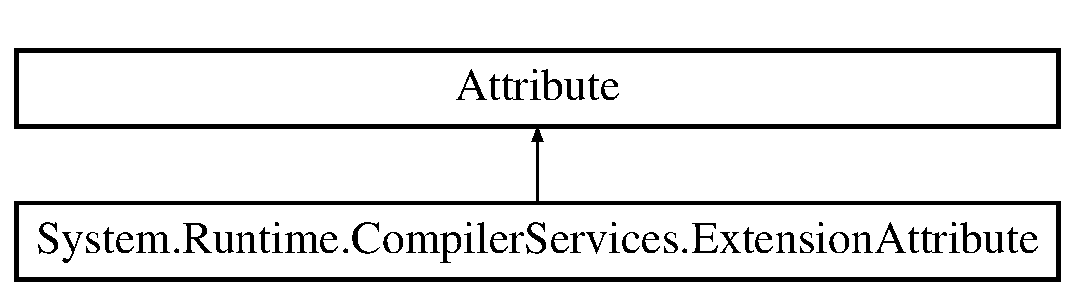
\includegraphics[height=2.000000cm]{class_system_1_1_runtime_1_1_compiler_services_1_1_extension_attribute}
\end{center}
\end{figure}


\subsection{详细描述}


在文件 Tree\-Item.\-cs 第 34 行定义.



该类的文档由以下文件生成\-:\begin{DoxyCompactItemize}
\item 
D\-:/\-My\-Data/\-My\-Git/\-Git\-Hub/\-X\-C\-L\-Net\-Tools/\-X\-C\-L\-Net\-Tools/\-Entity/\-Easy\-U\-I/\hyperlink{_tree_item_8cs}{Tree\-Item.\-cs}\end{DoxyCompactItemize}

\hypertarget{class_x_c_l_net_tools_1_1_file_handler_1_1_file_directory}{}\section{X\+C\+L\+Net\+Tools.\+File\+Handler.\+File\+Directory类 参考}
\label{class_x_c_l_net_tools_1_1_file_handler_1_1_file_directory}\index{X\+C\+L\+Net\+Tools.\+File\+Handler.\+File\+Directory@{X\+C\+L\+Net\+Tools.\+File\+Handler.\+File\+Directory}}


文件目录操作类  


\subsection*{静态 Public 成员函数}
\begin{DoxyCompactItemize}
\item 
static bool \hyperlink{class_x_c_l_net_tools_1_1_file_handler_1_1_file_directory_ac644b5cfdbc06559b2691ca6751506df}{Is\+Empty} (string path)
\begin{DoxyCompactList}\small\item\em 检测目录是否为空目录(既没有文件夹,也没有文件) \end{DoxyCompactList}\item 
static bool \hyperlink{class_x_c_l_net_tools_1_1_file_handler_1_1_file_directory_a1bc5d74fb797d8f8271caf1601f428fe}{Directory\+Exists} (string directory\+Name)
\begin{DoxyCompactList}\small\item\em 判断目录是否存在 \end{DoxyCompactList}\item 
static bool \hyperlink{class_x_c_l_net_tools_1_1_file_handler_1_1_file_directory_a8f3ce048a9225a0b699d7bbc510bd9e3}{Make\+Directory} (string directory\+Name)
\begin{DoxyCompactList}\small\item\em 建立目录 \end{DoxyCompactList}\item 
static bool \hyperlink{class_x_c_l_net_tools_1_1_file_handler_1_1_file_directory_aea79f469e66f1668c6bb4eff61bf9279}{R\+M\+D\+IR} (string directory\+Name)
\begin{DoxyCompactList}\small\item\em 删除指定的目录 \end{DoxyCompactList}\item 
static bool \hyperlink{class_x_c_l_net_tools_1_1_file_handler_1_1_file_directory_a1810da560c803121e71fa92fd4f9d180}{Del\+Tree} (string directory\+Name)
\begin{DoxyCompactList}\small\item\em 删除目录并删除其下的子目录及其文件 \end{DoxyCompactList}\item 
static bool \hyperlink{class_x_c_l_net_tools_1_1_file_handler_1_1_file_directory_a1f64c69d3e2dc580b54a93fe0c871178}{Clear\+Directory} (string root\+Path)
\begin{DoxyCompactList}\small\item\em 清空指定目录 \end{DoxyCompactList}\item 
static List$<$ \hyperlink{class_x_c_l_net_tools_1_1_entity_1_1_file_info_entity}{X\+C\+L\+Net\+Tools.\+Entity.\+File\+Info\+Entity} $>$ \hyperlink{class_x_c_l_net_tools_1_1_file_handler_1_1_file_directory_ac145cab935d17a93ec683d1763bfdccd}{Get\+File\+List} (string dir\+Path, string root\+Path=\char`\"{}\char`\"{}, string web\+Root\+Path=\char`\"{}\char`\"{})
\begin{DoxyCompactList}\small\item\em 获取指定目录下的所有文件及文件夹信息 \end{DoxyCompactList}\item 
static bool \hyperlink{class_x_c_l_net_tools_1_1_file_handler_1_1_file_directory_a40110c2de9ef47ac099acdbbf0703a0c}{Create\+Text\+File} (string file\+Path\+Name)
\begin{DoxyCompactList}\small\item\em 建立一个文件 \end{DoxyCompactList}\item 
static void \hyperlink{class_x_c_l_net_tools_1_1_file_handler_1_1_file_directory_a7153ad7012f2c7259a89cc1f44fa57e2}{Append\+Text} (string file\+Path\+Name, string write\+Word)
\begin{DoxyCompactList}\small\item\em 在文件里追加内容 \end{DoxyCompactList}\item 
static void \hyperlink{class_x_c_l_net_tools_1_1_file_handler_1_1_file_directory_a15ae657816572db98e886f45b2949f76}{Append\+Text} (string file\+Path\+Name, string write\+Word, System.\+Text.\+Encoding encode)
\begin{DoxyCompactList}\small\item\em 在文件里追加内容 \end{DoxyCompactList}\item 
static string \hyperlink{class_x_c_l_net_tools_1_1_file_handler_1_1_file_directory_a5658b6c4ee9c9d4035033e5eb5ac773b}{Read\+File\+Data} (string file\+Path\+Name)
\begin{DoxyCompactList}\small\item\em 读取文件里内容 \end{DoxyCompactList}\item 
static bool \hyperlink{class_x_c_l_net_tools_1_1_file_handler_1_1_file_directory_a8ce6f5c7bf94c4fe2770993cef7be536}{File\+Delete} (string absolute\+File\+Path)
\begin{DoxyCompactList}\small\item\em 删除文件 \end{DoxyCompactList}\end{DoxyCompactItemize}


\subsection{详细描述}
文件目录操作类 



在文件 File\+Directory.\+cs 第 18 行定义.



\subsection{成员函数说明}
\index{X\+C\+L\+Net\+Tools\+::\+File\+Handler\+::\+File\+Directory@{X\+C\+L\+Net\+Tools\+::\+File\+Handler\+::\+File\+Directory}!Append\+Text@{Append\+Text}}
\index{Append\+Text@{Append\+Text}!X\+C\+L\+Net\+Tools\+::\+File\+Handler\+::\+File\+Directory@{X\+C\+L\+Net\+Tools\+::\+File\+Handler\+::\+File\+Directory}}
\subsubsection[{\texorpdfstring{Append\+Text(string file\+Path\+Name, string write\+Word)}{AppendText(string filePathName, string writeWord)}}]{\setlength{\rightskip}{0pt plus 5cm}static void X\+C\+L\+Net\+Tools.\+File\+Handler.\+File\+Directory.\+Append\+Text (
\begin{DoxyParamCaption}
\item[{string}]{file\+Path\+Name, }
\item[{string}]{write\+Word}
\end{DoxyParamCaption}
)\hspace{0.3cm}{\ttfamily [static]}}\hypertarget{class_x_c_l_net_tools_1_1_file_handler_1_1_file_directory_a7153ad7012f2c7259a89cc1f44fa57e2}{}\label{class_x_c_l_net_tools_1_1_file_handler_1_1_file_directory_a7153ad7012f2c7259a89cc1f44fa57e2}


在文件里追加内容 


\begin{DoxyParams}{参数}
{\em file\+Path\+Name} & 文件名\\
\hline
{\em write\+Word} & 追加内容\\
\hline
\end{DoxyParams}


在文件 File\+Directory.\+cs 第 245 行定义.

\index{X\+C\+L\+Net\+Tools\+::\+File\+Handler\+::\+File\+Directory@{X\+C\+L\+Net\+Tools\+::\+File\+Handler\+::\+File\+Directory}!Append\+Text@{Append\+Text}}
\index{Append\+Text@{Append\+Text}!X\+C\+L\+Net\+Tools\+::\+File\+Handler\+::\+File\+Directory@{X\+C\+L\+Net\+Tools\+::\+File\+Handler\+::\+File\+Directory}}
\subsubsection[{\texorpdfstring{Append\+Text(string file\+Path\+Name, string write\+Word, System.\+Text.\+Encoding encode)}{AppendText(string filePathName, string writeWord, System.Text.Encoding encode)}}]{\setlength{\rightskip}{0pt plus 5cm}static void X\+C\+L\+Net\+Tools.\+File\+Handler.\+File\+Directory.\+Append\+Text (
\begin{DoxyParamCaption}
\item[{string}]{file\+Path\+Name, }
\item[{string}]{write\+Word, }
\item[{System.\+Text.\+Encoding}]{encode}
\end{DoxyParamCaption}
)\hspace{0.3cm}{\ttfamily [static]}}\hypertarget{class_x_c_l_net_tools_1_1_file_handler_1_1_file_directory_a15ae657816572db98e886f45b2949f76}{}\label{class_x_c_l_net_tools_1_1_file_handler_1_1_file_directory_a15ae657816572db98e886f45b2949f76}


在文件里追加内容 


\begin{DoxyParams}{参数}
{\em file\+Path\+Name} & 文件名\\
\hline
{\em write\+Word} & 追加内容\\
\hline
{\em encode} & 编码\\
\hline
\end{DoxyParams}


在文件 File\+Directory.\+cs 第 256 行定义.

\index{X\+C\+L\+Net\+Tools\+::\+File\+Handler\+::\+File\+Directory@{X\+C\+L\+Net\+Tools\+::\+File\+Handler\+::\+File\+Directory}!Clear\+Directory@{Clear\+Directory}}
\index{Clear\+Directory@{Clear\+Directory}!X\+C\+L\+Net\+Tools\+::\+File\+Handler\+::\+File\+Directory@{X\+C\+L\+Net\+Tools\+::\+File\+Handler\+::\+File\+Directory}}
\subsubsection[{\texorpdfstring{Clear\+Directory(string root\+Path)}{ClearDirectory(string rootPath)}}]{\setlength{\rightskip}{0pt plus 5cm}static bool X\+C\+L\+Net\+Tools.\+File\+Handler.\+File\+Directory.\+Clear\+Directory (
\begin{DoxyParamCaption}
\item[{string}]{root\+Path}
\end{DoxyParamCaption}
)\hspace{0.3cm}{\ttfamily [static]}}\hypertarget{class_x_c_l_net_tools_1_1_file_handler_1_1_file_directory_a1f64c69d3e2dc580b54a93fe0c871178}{}\label{class_x_c_l_net_tools_1_1_file_handler_1_1_file_directory_a1f64c69d3e2dc580b54a93fe0c871178}


清空指定目录 


\begin{DoxyParams}{参数}
{\em root\+Path} & 要清空的目录\\
\hline
\end{DoxyParams}
\begin{DoxyReturn}{返回}
是否操作成功
\end{DoxyReturn}


在文件 File\+Directory.\+cs 第 115 行定义.

\index{X\+C\+L\+Net\+Tools\+::\+File\+Handler\+::\+File\+Directory@{X\+C\+L\+Net\+Tools\+::\+File\+Handler\+::\+File\+Directory}!Create\+Text\+File@{Create\+Text\+File}}
\index{Create\+Text\+File@{Create\+Text\+File}!X\+C\+L\+Net\+Tools\+::\+File\+Handler\+::\+File\+Directory@{X\+C\+L\+Net\+Tools\+::\+File\+Handler\+::\+File\+Directory}}
\subsubsection[{\texorpdfstring{Create\+Text\+File(string file\+Path\+Name)}{CreateTextFile(string filePathName)}}]{\setlength{\rightskip}{0pt plus 5cm}static bool X\+C\+L\+Net\+Tools.\+File\+Handler.\+File\+Directory.\+Create\+Text\+File (
\begin{DoxyParamCaption}
\item[{string}]{file\+Path\+Name}
\end{DoxyParamCaption}
)\hspace{0.3cm}{\ttfamily [static]}}\hypertarget{class_x_c_l_net_tools_1_1_file_handler_1_1_file_directory_a40110c2de9ef47ac099acdbbf0703a0c}{}\label{class_x_c_l_net_tools_1_1_file_handler_1_1_file_directory_a40110c2de9ef47ac099acdbbf0703a0c}


建立一个文件 


\begin{DoxyParams}{参数}
{\em file\+Path\+Name} & 目录名\\
\hline
\end{DoxyParams}
\begin{DoxyReturn}{返回}
true\+:建立成功,false\+:建立失败
\end{DoxyReturn}


在文件 File\+Directory.\+cs 第 223 行定义.

\index{X\+C\+L\+Net\+Tools\+::\+File\+Handler\+::\+File\+Directory@{X\+C\+L\+Net\+Tools\+::\+File\+Handler\+::\+File\+Directory}!Del\+Tree@{Del\+Tree}}
\index{Del\+Tree@{Del\+Tree}!X\+C\+L\+Net\+Tools\+::\+File\+Handler\+::\+File\+Directory@{X\+C\+L\+Net\+Tools\+::\+File\+Handler\+::\+File\+Directory}}
\subsubsection[{\texorpdfstring{Del\+Tree(string directory\+Name)}{DelTree(string directoryName)}}]{\setlength{\rightskip}{0pt plus 5cm}static bool X\+C\+L\+Net\+Tools.\+File\+Handler.\+File\+Directory.\+Del\+Tree (
\begin{DoxyParamCaption}
\item[{string}]{directory\+Name}
\end{DoxyParamCaption}
)\hspace{0.3cm}{\ttfamily [static]}}\hypertarget{class_x_c_l_net_tools_1_1_file_handler_1_1_file_directory_a1810da560c803121e71fa92fd4f9d180}{}\label{class_x_c_l_net_tools_1_1_file_handler_1_1_file_directory_a1810da560c803121e71fa92fd4f9d180}


删除目录并删除其下的子目录及其文件 


\begin{DoxyParams}{参数}
{\em directory\+Name} & 目录名\\
\hline
\end{DoxyParams}
\begin{DoxyReturn}{返回}
true\+:删除成功,false\+:删除失败
\end{DoxyReturn}


在文件 File\+Directory.\+cs 第 97 行定义.

\index{X\+C\+L\+Net\+Tools\+::\+File\+Handler\+::\+File\+Directory@{X\+C\+L\+Net\+Tools\+::\+File\+Handler\+::\+File\+Directory}!Directory\+Exists@{Directory\+Exists}}
\index{Directory\+Exists@{Directory\+Exists}!X\+C\+L\+Net\+Tools\+::\+File\+Handler\+::\+File\+Directory@{X\+C\+L\+Net\+Tools\+::\+File\+Handler\+::\+File\+Directory}}
\subsubsection[{\texorpdfstring{Directory\+Exists(string directory\+Name)}{DirectoryExists(string directoryName)}}]{\setlength{\rightskip}{0pt plus 5cm}static bool X\+C\+L\+Net\+Tools.\+File\+Handler.\+File\+Directory.\+Directory\+Exists (
\begin{DoxyParamCaption}
\item[{string}]{directory\+Name}
\end{DoxyParamCaption}
)\hspace{0.3cm}{\ttfamily [static]}}\hypertarget{class_x_c_l_net_tools_1_1_file_handler_1_1_file_directory_a1bc5d74fb797d8f8271caf1601f428fe}{}\label{class_x_c_l_net_tools_1_1_file_handler_1_1_file_directory_a1bc5d74fb797d8f8271caf1601f428fe}


判断目录是否存在 


\begin{DoxyParams}{参数}
{\em directory\+Name} & 目录路径\\
\hline
\end{DoxyParams}
\begin{DoxyReturn}{返回}
true:存在,false:不存在
\end{DoxyReturn}


在文件 File\+Directory.\+cs 第 43 行定义.

\index{X\+C\+L\+Net\+Tools\+::\+File\+Handler\+::\+File\+Directory@{X\+C\+L\+Net\+Tools\+::\+File\+Handler\+::\+File\+Directory}!File\+Delete@{File\+Delete}}
\index{File\+Delete@{File\+Delete}!X\+C\+L\+Net\+Tools\+::\+File\+Handler\+::\+File\+Directory@{X\+C\+L\+Net\+Tools\+::\+File\+Handler\+::\+File\+Directory}}
\subsubsection[{\texorpdfstring{File\+Delete(string absolute\+File\+Path)}{FileDelete(string absoluteFilePath)}}]{\setlength{\rightskip}{0pt plus 5cm}static bool X\+C\+L\+Net\+Tools.\+File\+Handler.\+File\+Directory.\+File\+Delete (
\begin{DoxyParamCaption}
\item[{string}]{absolute\+File\+Path}
\end{DoxyParamCaption}
)\hspace{0.3cm}{\ttfamily [static]}}\hypertarget{class_x_c_l_net_tools_1_1_file_handler_1_1_file_directory_a8ce6f5c7bf94c4fe2770993cef7be536}{}\label{class_x_c_l_net_tools_1_1_file_handler_1_1_file_directory_a8ce6f5c7bf94c4fe2770993cef7be536}


删除文件 


\begin{DoxyParams}{参数}
{\em absolute\+File\+Path} & 文件绝对地址\\
\hline
\end{DoxyParams}
\begin{DoxyReturn}{返回}
true\+:删除文件成功,false\+:删除文件失败
\end{DoxyReturn}


在文件 File\+Directory.\+cs 第 292 行定义.

\index{X\+C\+L\+Net\+Tools\+::\+File\+Handler\+::\+File\+Directory@{X\+C\+L\+Net\+Tools\+::\+File\+Handler\+::\+File\+Directory}!Get\+File\+List@{Get\+File\+List}}
\index{Get\+File\+List@{Get\+File\+List}!X\+C\+L\+Net\+Tools\+::\+File\+Handler\+::\+File\+Directory@{X\+C\+L\+Net\+Tools\+::\+File\+Handler\+::\+File\+Directory}}
\subsubsection[{\texorpdfstring{Get\+File\+List(string dir\+Path, string root\+Path="""", string web\+Root\+Path="""")}{GetFileList(string dirPath, string rootPath="", string webRootPath="")}}]{\setlength{\rightskip}{0pt plus 5cm}static List$<${\bf X\+C\+L\+Net\+Tools.\+Entity.\+File\+Info\+Entity}$>$ X\+C\+L\+Net\+Tools.\+File\+Handler.\+File\+Directory.\+Get\+File\+List (
\begin{DoxyParamCaption}
\item[{string}]{dir\+Path, }
\item[{string}]{root\+Path = {\ttfamily \char`\"{}\char`\"{}}, }
\item[{string}]{web\+Root\+Path = {\ttfamily \char`\"{}\char`\"{}}}
\end{DoxyParamCaption}
)\hspace{0.3cm}{\ttfamily [static]}}\hypertarget{class_x_c_l_net_tools_1_1_file_handler_1_1_file_directory_ac145cab935d17a93ec683d1763bfdccd}{}\label{class_x_c_l_net_tools_1_1_file_handler_1_1_file_directory_ac145cab935d17a93ec683d1763bfdccd}


获取指定目录下的所有文件及文件夹信息 


\begin{DoxyParams}{参数}
{\em dir\+Path} & 要获取信息的目录路径\\
\hline
{\em root\+Path} & 根路径(设置该值后,返回的信息实体中将包含相对于该根路径的相对路径信息)\\
\hline
{\em web\+Root\+Path} & web根路径(用于生成该文件或文件夹的web路径),如:http\+://www.a.\+com/web/\\
\hline
\end{DoxyParams}
\begin{DoxyReturn}{返回}
文件信息list
\end{DoxyReturn}


在文件 File\+Directory.\+cs 第 142 行定义.

\index{X\+C\+L\+Net\+Tools\+::\+File\+Handler\+::\+File\+Directory@{X\+C\+L\+Net\+Tools\+::\+File\+Handler\+::\+File\+Directory}!Is\+Empty@{Is\+Empty}}
\index{Is\+Empty@{Is\+Empty}!X\+C\+L\+Net\+Tools\+::\+File\+Handler\+::\+File\+Directory@{X\+C\+L\+Net\+Tools\+::\+File\+Handler\+::\+File\+Directory}}
\subsubsection[{\texorpdfstring{Is\+Empty(string path)}{IsEmpty(string path)}}]{\setlength{\rightskip}{0pt plus 5cm}static bool X\+C\+L\+Net\+Tools.\+File\+Handler.\+File\+Directory.\+Is\+Empty (
\begin{DoxyParamCaption}
\item[{string}]{path}
\end{DoxyParamCaption}
)\hspace{0.3cm}{\ttfamily [static]}}\hypertarget{class_x_c_l_net_tools_1_1_file_handler_1_1_file_directory_ac644b5cfdbc06559b2691ca6751506df}{}\label{class_x_c_l_net_tools_1_1_file_handler_1_1_file_directory_ac644b5cfdbc06559b2691ca6751506df}


检测目录是否为空目录(既没有文件夹,也没有文件) 


\begin{DoxyParams}{参数}
{\em path} & 目录路径\\
\hline
\end{DoxyParams}
\begin{DoxyReturn}{返回}
true\+:空目录,false\+:非空目录
\end{DoxyReturn}


在文件 File\+Directory.\+cs 第 27 行定义.

\index{X\+C\+L\+Net\+Tools\+::\+File\+Handler\+::\+File\+Directory@{X\+C\+L\+Net\+Tools\+::\+File\+Handler\+::\+File\+Directory}!Make\+Directory@{Make\+Directory}}
\index{Make\+Directory@{Make\+Directory}!X\+C\+L\+Net\+Tools\+::\+File\+Handler\+::\+File\+Directory@{X\+C\+L\+Net\+Tools\+::\+File\+Handler\+::\+File\+Directory}}
\subsubsection[{\texorpdfstring{Make\+Directory(string directory\+Name)}{MakeDirectory(string directoryName)}}]{\setlength{\rightskip}{0pt plus 5cm}static bool X\+C\+L\+Net\+Tools.\+File\+Handler.\+File\+Directory.\+Make\+Directory (
\begin{DoxyParamCaption}
\item[{string}]{directory\+Name}
\end{DoxyParamCaption}
)\hspace{0.3cm}{\ttfamily [static]}}\hypertarget{class_x_c_l_net_tools_1_1_file_handler_1_1_file_directory_a8f3ce048a9225a0b699d7bbc510bd9e3}{}\label{class_x_c_l_net_tools_1_1_file_handler_1_1_file_directory_a8f3ce048a9225a0b699d7bbc510bd9e3}


建立目录 


\begin{DoxyParams}{参数}
{\em directory\+Name} & 目录名\\
\hline
\end{DoxyParams}
\begin{DoxyReturn}{返回}
返回boolean,true\+:目录建立成功, false\+:目录建立失败
\end{DoxyReturn}


在文件 File\+Directory.\+cs 第 53 行定义.

\index{X\+C\+L\+Net\+Tools\+::\+File\+Handler\+::\+File\+Directory@{X\+C\+L\+Net\+Tools\+::\+File\+Handler\+::\+File\+Directory}!Read\+File\+Data@{Read\+File\+Data}}
\index{Read\+File\+Data@{Read\+File\+Data}!X\+C\+L\+Net\+Tools\+::\+File\+Handler\+::\+File\+Directory@{X\+C\+L\+Net\+Tools\+::\+File\+Handler\+::\+File\+Directory}}
\subsubsection[{\texorpdfstring{Read\+File\+Data(string file\+Path\+Name)}{ReadFileData(string filePathName)}}]{\setlength{\rightskip}{0pt plus 5cm}static string X\+C\+L\+Net\+Tools.\+File\+Handler.\+File\+Directory.\+Read\+File\+Data (
\begin{DoxyParamCaption}
\item[{string}]{file\+Path\+Name}
\end{DoxyParamCaption}
)\hspace{0.3cm}{\ttfamily [static]}}\hypertarget{class_x_c_l_net_tools_1_1_file_handler_1_1_file_directory_a5658b6c4ee9c9d4035033e5eb5ac773b}{}\label{class_x_c_l_net_tools_1_1_file_handler_1_1_file_directory_a5658b6c4ee9c9d4035033e5eb5ac773b}


读取文件里内容 


\begin{DoxyParams}{参数}
{\em file\+Path\+Name} & 文件名\\
\hline
\end{DoxyParams}
\begin{DoxyReturn}{返回}
文件内容
\end{DoxyReturn}


在文件 File\+Directory.\+cs 第 276 行定义.

\index{X\+C\+L\+Net\+Tools\+::\+File\+Handler\+::\+File\+Directory@{X\+C\+L\+Net\+Tools\+::\+File\+Handler\+::\+File\+Directory}!R\+M\+D\+IR@{R\+M\+D\+IR}}
\index{R\+M\+D\+IR@{R\+M\+D\+IR}!X\+C\+L\+Net\+Tools\+::\+File\+Handler\+::\+File\+Directory@{X\+C\+L\+Net\+Tools\+::\+File\+Handler\+::\+File\+Directory}}
\subsubsection[{\texorpdfstring{R\+M\+D\+I\+R(string directory\+Name)}{RMDIR(string directoryName)}}]{\setlength{\rightskip}{0pt plus 5cm}static bool X\+C\+L\+Net\+Tools.\+File\+Handler.\+File\+Directory.\+R\+M\+D\+IR (
\begin{DoxyParamCaption}
\item[{string}]{directory\+Name}
\end{DoxyParamCaption}
)\hspace{0.3cm}{\ttfamily [static]}}\hypertarget{class_x_c_l_net_tools_1_1_file_handler_1_1_file_directory_aea79f469e66f1668c6bb4eff61bf9279}{}\label{class_x_c_l_net_tools_1_1_file_handler_1_1_file_directory_aea79f469e66f1668c6bb4eff61bf9279}


删除指定的目录 


\begin{DoxyParams}{参数}
{\em directory\+Name} & 目录名\\
\hline
\end{DoxyParams}
\begin{DoxyReturn}{返回}
true:删除成功,false:删除失败
\end{DoxyReturn}


在文件 File\+Directory.\+cs 第 78 行定义.



该类的文档由以下文件生成\+:\begin{DoxyCompactItemize}
\item 
E\+:/\+Git\+Hub/\+X\+C\+L\+Net\+Tools/\+X\+C\+L\+Net\+Tools/\+File\+Handler/\hyperlink{_file_directory_8cs}{File\+Directory.\+cs}\end{DoxyCompactItemize}

\hypertarget{class_x_c_l_net_tools_1_1_entity_1_1_file_info_entity}{}\section{X\+C\+L\+Net\+Tools.\+Entity.\+File\+Info\+Entity类 参考}
\label{class_x_c_l_net_tools_1_1_entity_1_1_file_info_entity}\index{X\+C\+L\+Net\+Tools.\+Entity.\+File\+Info\+Entity@{X\+C\+L\+Net\+Tools.\+Entity.\+File\+Info\+Entity}}


文件信息实体  


\subsection*{属性}
\begin{DoxyCompactItemize}
\item 
int \hyperlink{class_x_c_l_net_tools_1_1_entity_1_1_file_info_entity_a150f26081f12badeea9a2255bbea6faf}{ID}\hspace{0.3cm}{\ttfamily  \mbox{[}get, set\mbox{]}}
\begin{DoxyCompactList}\small\item\em 标识\+ID \end{DoxyCompactList}\item 
bool \hyperlink{class_x_c_l_net_tools_1_1_entity_1_1_file_info_entity_ad945716535742c01f83dffc2766c0987}{Is\+Folder}\hspace{0.3cm}{\ttfamily  \mbox{[}get, set\mbox{]}}
\begin{DoxyCompactList}\small\item\em 是否为文件夹 \end{DoxyCompactList}\item 
string \hyperlink{class_x_c_l_net_tools_1_1_entity_1_1_file_info_entity_a15a2bb6c738c32250f00604b6636cae4}{Name}\hspace{0.3cm}{\ttfamily  \mbox{[}get, set\mbox{]}}
\begin{DoxyCompactList}\small\item\em 文件名 \end{DoxyCompactList}\item 
string \hyperlink{class_x_c_l_net_tools_1_1_entity_1_1_file_info_entity_a46ccaf5dbcc1154782c0227c83eb54e4}{Ext\+Name}\hspace{0.3cm}{\ttfamily  \mbox{[}get, set\mbox{]}}
\begin{DoxyCompactList}\small\item\em 扩展名(不含小圆点) \end{DoxyCompactList}\item 
string \hyperlink{class_x_c_l_net_tools_1_1_entity_1_1_file_info_entity_a6ef4c659747c605379a43168ae1d64f6}{Root\+Path}\hspace{0.3cm}{\ttfamily  \mbox{[}get, set\mbox{]}}
\begin{DoxyCompactList}\small\item\em 根物理路径 \end{DoxyCompactList}\item 
string \hyperlink{class_x_c_l_net_tools_1_1_entity_1_1_file_info_entity_a67f485c1a1af6205351305756d515e98}{Path}\hspace{0.3cm}{\ttfamily  \mbox{[}get, set\mbox{]}}
\begin{DoxyCompactList}\small\item\em 该文件或文件夹的物理路径 \end{DoxyCompactList}\item 
string \hyperlink{class_x_c_l_net_tools_1_1_entity_1_1_file_info_entity_ab93bd802770bb40cc0abdfd35d2fbbc6}{Web\+Path}\hspace{0.3cm}{\ttfamily  \mbox{[}get, set\mbox{]}}
\begin{DoxyCompactList}\small\item\em 该文件或文件夹的web路径 \end{DoxyCompactList}\item 
string \hyperlink{class_x_c_l_net_tools_1_1_entity_1_1_file_info_entity_a795982d186fa2d1ef0e3fb51705f36b2}{Relative\+Path}\hspace{0.3cm}{\ttfamily  \mbox{[}get, set\mbox{]}}
\begin{DoxyCompactList}\small\item\em 该文件或文件夹相对于\+Root\+Path的相对路径 \end{DoxyCompactList}\item 
long \hyperlink{class_x_c_l_net_tools_1_1_entity_1_1_file_info_entity_a7447a43994e75793388e160a626ba346}{Size}\hspace{0.3cm}{\ttfamily  \mbox{[}get, set\mbox{]}}
\begin{DoxyCompactList}\small\item\em 大小(byte) \end{DoxyCompactList}\item 
Date\+Time \hyperlink{class_x_c_l_net_tools_1_1_entity_1_1_file_info_entity_a64c6633bec7e4d547632c122dbaad9f8}{Modify\+Time}\hspace{0.3cm}{\ttfamily  \mbox{[}get, set\mbox{]}}
\begin{DoxyCompactList}\small\item\em 修改时间 \end{DoxyCompactList}\item 
Date\+Time \hyperlink{class_x_c_l_net_tools_1_1_entity_1_1_file_info_entity_a93fc7b2a3119885d9449d1817e7306ca}{Create\+Time}\hspace{0.3cm}{\ttfamily  \mbox{[}get, set\mbox{]}}
\begin{DoxyCompactList}\small\item\em 创建时间 \end{DoxyCompactList}\end{DoxyCompactItemize}


\subsection{详细描述}
文件信息实体 



在文件 File\+Info\+Entity.\+cs 第 17 行定义.



\subsection{属性说明}
\index{X\+C\+L\+Net\+Tools\+::\+Entity\+::\+File\+Info\+Entity@{X\+C\+L\+Net\+Tools\+::\+Entity\+::\+File\+Info\+Entity}!Create\+Time@{Create\+Time}}
\index{Create\+Time@{Create\+Time}!X\+C\+L\+Net\+Tools\+::\+Entity\+::\+File\+Info\+Entity@{X\+C\+L\+Net\+Tools\+::\+Entity\+::\+File\+Info\+Entity}}
\subsubsection[{\texorpdfstring{Create\+Time}{CreateTime}}]{\setlength{\rightskip}{0pt plus 5cm}Date\+Time X\+C\+L\+Net\+Tools.\+Entity.\+File\+Info\+Entity.\+Create\+Time\hspace{0.3cm}{\ttfamily [get]}, {\ttfamily [set]}}\hypertarget{class_x_c_l_net_tools_1_1_entity_1_1_file_info_entity_a93fc7b2a3119885d9449d1817e7306ca}{}\label{class_x_c_l_net_tools_1_1_entity_1_1_file_info_entity_a93fc7b2a3119885d9449d1817e7306ca}


创建时间 



在文件 File\+Info\+Entity.\+cs 第 72 行定义.

\index{X\+C\+L\+Net\+Tools\+::\+Entity\+::\+File\+Info\+Entity@{X\+C\+L\+Net\+Tools\+::\+Entity\+::\+File\+Info\+Entity}!Ext\+Name@{Ext\+Name}}
\index{Ext\+Name@{Ext\+Name}!X\+C\+L\+Net\+Tools\+::\+Entity\+::\+File\+Info\+Entity@{X\+C\+L\+Net\+Tools\+::\+Entity\+::\+File\+Info\+Entity}}
\subsubsection[{\texorpdfstring{Ext\+Name}{ExtName}}]{\setlength{\rightskip}{0pt plus 5cm}string X\+C\+L\+Net\+Tools.\+Entity.\+File\+Info\+Entity.\+Ext\+Name\hspace{0.3cm}{\ttfamily [get]}, {\ttfamily [set]}}\hypertarget{class_x_c_l_net_tools_1_1_entity_1_1_file_info_entity_a46ccaf5dbcc1154782c0227c83eb54e4}{}\label{class_x_c_l_net_tools_1_1_entity_1_1_file_info_entity_a46ccaf5dbcc1154782c0227c83eb54e4}


扩展名(不含小圆点) 



在文件 File\+Info\+Entity.\+cs 第 37 行定义.

\index{X\+C\+L\+Net\+Tools\+::\+Entity\+::\+File\+Info\+Entity@{X\+C\+L\+Net\+Tools\+::\+Entity\+::\+File\+Info\+Entity}!ID@{ID}}
\index{ID@{ID}!X\+C\+L\+Net\+Tools\+::\+Entity\+::\+File\+Info\+Entity@{X\+C\+L\+Net\+Tools\+::\+Entity\+::\+File\+Info\+Entity}}
\subsubsection[{\texorpdfstring{ID}{ID}}]{\setlength{\rightskip}{0pt plus 5cm}int X\+C\+L\+Net\+Tools.\+Entity.\+File\+Info\+Entity.\+ID\hspace{0.3cm}{\ttfamily [get]}, {\ttfamily [set]}}\hypertarget{class_x_c_l_net_tools_1_1_entity_1_1_file_info_entity_a150f26081f12badeea9a2255bbea6faf}{}\label{class_x_c_l_net_tools_1_1_entity_1_1_file_info_entity_a150f26081f12badeea9a2255bbea6faf}


标识\+ID 



在文件 File\+Info\+Entity.\+cs 第 22 行定义.

\index{X\+C\+L\+Net\+Tools\+::\+Entity\+::\+File\+Info\+Entity@{X\+C\+L\+Net\+Tools\+::\+Entity\+::\+File\+Info\+Entity}!Is\+Folder@{Is\+Folder}}
\index{Is\+Folder@{Is\+Folder}!X\+C\+L\+Net\+Tools\+::\+Entity\+::\+File\+Info\+Entity@{X\+C\+L\+Net\+Tools\+::\+Entity\+::\+File\+Info\+Entity}}
\subsubsection[{\texorpdfstring{Is\+Folder}{IsFolder}}]{\setlength{\rightskip}{0pt plus 5cm}bool X\+C\+L\+Net\+Tools.\+Entity.\+File\+Info\+Entity.\+Is\+Folder\hspace{0.3cm}{\ttfamily [get]}, {\ttfamily [set]}}\hypertarget{class_x_c_l_net_tools_1_1_entity_1_1_file_info_entity_ad945716535742c01f83dffc2766c0987}{}\label{class_x_c_l_net_tools_1_1_entity_1_1_file_info_entity_ad945716535742c01f83dffc2766c0987}


是否为文件夹 



在文件 File\+Info\+Entity.\+cs 第 27 行定义.

\index{X\+C\+L\+Net\+Tools\+::\+Entity\+::\+File\+Info\+Entity@{X\+C\+L\+Net\+Tools\+::\+Entity\+::\+File\+Info\+Entity}!Modify\+Time@{Modify\+Time}}
\index{Modify\+Time@{Modify\+Time}!X\+C\+L\+Net\+Tools\+::\+Entity\+::\+File\+Info\+Entity@{X\+C\+L\+Net\+Tools\+::\+Entity\+::\+File\+Info\+Entity}}
\subsubsection[{\texorpdfstring{Modify\+Time}{ModifyTime}}]{\setlength{\rightskip}{0pt plus 5cm}Date\+Time X\+C\+L\+Net\+Tools.\+Entity.\+File\+Info\+Entity.\+Modify\+Time\hspace{0.3cm}{\ttfamily [get]}, {\ttfamily [set]}}\hypertarget{class_x_c_l_net_tools_1_1_entity_1_1_file_info_entity_a64c6633bec7e4d547632c122dbaad9f8}{}\label{class_x_c_l_net_tools_1_1_entity_1_1_file_info_entity_a64c6633bec7e4d547632c122dbaad9f8}


修改时间 



在文件 File\+Info\+Entity.\+cs 第 67 行定义.

\index{X\+C\+L\+Net\+Tools\+::\+Entity\+::\+File\+Info\+Entity@{X\+C\+L\+Net\+Tools\+::\+Entity\+::\+File\+Info\+Entity}!Name@{Name}}
\index{Name@{Name}!X\+C\+L\+Net\+Tools\+::\+Entity\+::\+File\+Info\+Entity@{X\+C\+L\+Net\+Tools\+::\+Entity\+::\+File\+Info\+Entity}}
\subsubsection[{\texorpdfstring{Name}{Name}}]{\setlength{\rightskip}{0pt plus 5cm}string X\+C\+L\+Net\+Tools.\+Entity.\+File\+Info\+Entity.\+Name\hspace{0.3cm}{\ttfamily [get]}, {\ttfamily [set]}}\hypertarget{class_x_c_l_net_tools_1_1_entity_1_1_file_info_entity_a15a2bb6c738c32250f00604b6636cae4}{}\label{class_x_c_l_net_tools_1_1_entity_1_1_file_info_entity_a15a2bb6c738c32250f00604b6636cae4}


文件名 



在文件 File\+Info\+Entity.\+cs 第 32 行定义.

\index{X\+C\+L\+Net\+Tools\+::\+Entity\+::\+File\+Info\+Entity@{X\+C\+L\+Net\+Tools\+::\+Entity\+::\+File\+Info\+Entity}!Path@{Path}}
\index{Path@{Path}!X\+C\+L\+Net\+Tools\+::\+Entity\+::\+File\+Info\+Entity@{X\+C\+L\+Net\+Tools\+::\+Entity\+::\+File\+Info\+Entity}}
\subsubsection[{\texorpdfstring{Path}{Path}}]{\setlength{\rightskip}{0pt plus 5cm}string X\+C\+L\+Net\+Tools.\+Entity.\+File\+Info\+Entity.\+Path\hspace{0.3cm}{\ttfamily [get]}, {\ttfamily [set]}}\hypertarget{class_x_c_l_net_tools_1_1_entity_1_1_file_info_entity_a67f485c1a1af6205351305756d515e98}{}\label{class_x_c_l_net_tools_1_1_entity_1_1_file_info_entity_a67f485c1a1af6205351305756d515e98}


该文件或文件夹的物理路径 



在文件 File\+Info\+Entity.\+cs 第 47 行定义.

\index{X\+C\+L\+Net\+Tools\+::\+Entity\+::\+File\+Info\+Entity@{X\+C\+L\+Net\+Tools\+::\+Entity\+::\+File\+Info\+Entity}!Relative\+Path@{Relative\+Path}}
\index{Relative\+Path@{Relative\+Path}!X\+C\+L\+Net\+Tools\+::\+Entity\+::\+File\+Info\+Entity@{X\+C\+L\+Net\+Tools\+::\+Entity\+::\+File\+Info\+Entity}}
\subsubsection[{\texorpdfstring{Relative\+Path}{RelativePath}}]{\setlength{\rightskip}{0pt plus 5cm}string X\+C\+L\+Net\+Tools.\+Entity.\+File\+Info\+Entity.\+Relative\+Path\hspace{0.3cm}{\ttfamily [get]}, {\ttfamily [set]}}\hypertarget{class_x_c_l_net_tools_1_1_entity_1_1_file_info_entity_a795982d186fa2d1ef0e3fb51705f36b2}{}\label{class_x_c_l_net_tools_1_1_entity_1_1_file_info_entity_a795982d186fa2d1ef0e3fb51705f36b2}


该文件或文件夹相对于\+Root\+Path的相对路径 



在文件 File\+Info\+Entity.\+cs 第 57 行定义.

\index{X\+C\+L\+Net\+Tools\+::\+Entity\+::\+File\+Info\+Entity@{X\+C\+L\+Net\+Tools\+::\+Entity\+::\+File\+Info\+Entity}!Root\+Path@{Root\+Path}}
\index{Root\+Path@{Root\+Path}!X\+C\+L\+Net\+Tools\+::\+Entity\+::\+File\+Info\+Entity@{X\+C\+L\+Net\+Tools\+::\+Entity\+::\+File\+Info\+Entity}}
\subsubsection[{\texorpdfstring{Root\+Path}{RootPath}}]{\setlength{\rightskip}{0pt plus 5cm}string X\+C\+L\+Net\+Tools.\+Entity.\+File\+Info\+Entity.\+Root\+Path\hspace{0.3cm}{\ttfamily [get]}, {\ttfamily [set]}}\hypertarget{class_x_c_l_net_tools_1_1_entity_1_1_file_info_entity_a6ef4c659747c605379a43168ae1d64f6}{}\label{class_x_c_l_net_tools_1_1_entity_1_1_file_info_entity_a6ef4c659747c605379a43168ae1d64f6}


根物理路径 



在文件 File\+Info\+Entity.\+cs 第 42 行定义.

\index{X\+C\+L\+Net\+Tools\+::\+Entity\+::\+File\+Info\+Entity@{X\+C\+L\+Net\+Tools\+::\+Entity\+::\+File\+Info\+Entity}!Size@{Size}}
\index{Size@{Size}!X\+C\+L\+Net\+Tools\+::\+Entity\+::\+File\+Info\+Entity@{X\+C\+L\+Net\+Tools\+::\+Entity\+::\+File\+Info\+Entity}}
\subsubsection[{\texorpdfstring{Size}{Size}}]{\setlength{\rightskip}{0pt plus 5cm}long X\+C\+L\+Net\+Tools.\+Entity.\+File\+Info\+Entity.\+Size\hspace{0.3cm}{\ttfamily [get]}, {\ttfamily [set]}}\hypertarget{class_x_c_l_net_tools_1_1_entity_1_1_file_info_entity_a7447a43994e75793388e160a626ba346}{}\label{class_x_c_l_net_tools_1_1_entity_1_1_file_info_entity_a7447a43994e75793388e160a626ba346}


大小(byte) 



在文件 File\+Info\+Entity.\+cs 第 62 行定义.

\index{X\+C\+L\+Net\+Tools\+::\+Entity\+::\+File\+Info\+Entity@{X\+C\+L\+Net\+Tools\+::\+Entity\+::\+File\+Info\+Entity}!Web\+Path@{Web\+Path}}
\index{Web\+Path@{Web\+Path}!X\+C\+L\+Net\+Tools\+::\+Entity\+::\+File\+Info\+Entity@{X\+C\+L\+Net\+Tools\+::\+Entity\+::\+File\+Info\+Entity}}
\subsubsection[{\texorpdfstring{Web\+Path}{WebPath}}]{\setlength{\rightskip}{0pt plus 5cm}string X\+C\+L\+Net\+Tools.\+Entity.\+File\+Info\+Entity.\+Web\+Path\hspace{0.3cm}{\ttfamily [get]}, {\ttfamily [set]}}\hypertarget{class_x_c_l_net_tools_1_1_entity_1_1_file_info_entity_ab93bd802770bb40cc0abdfd35d2fbbc6}{}\label{class_x_c_l_net_tools_1_1_entity_1_1_file_info_entity_ab93bd802770bb40cc0abdfd35d2fbbc6}


该文件或文件夹的web路径 



在文件 File\+Info\+Entity.\+cs 第 52 行定义.



该类的文档由以下文件生成\+:\begin{DoxyCompactItemize}
\item 
E\+:/\+Git\+Hub/\+X\+C\+L\+Net\+Tools/\+X\+C\+L\+Net\+Tools/\+Entity/\hyperlink{_file_info_entity_8cs}{File\+Info\+Entity.\+cs}\end{DoxyCompactItemize}

\hypertarget{class_x_c_l_net_tools_1_1_string_hander_1_1_form_helper}{\section{X\-C\-L\-Net\-Tools.\-String\-Hander.\-Form\-Helper类 参考}
\label{class_x_c_l_net_tools_1_1_string_hander_1_1_form_helper}\index{X\-C\-L\-Net\-Tools.\-String\-Hander.\-Form\-Helper@{X\-C\-L\-Net\-Tools.\-String\-Hander.\-Form\-Helper}}
}


form表单相关  


\subsection*{静态 Public 成员函数}
\begin{DoxyCompactItemize}
\item 
static string \hyperlink{class_x_c_l_net_tools_1_1_string_hander_1_1_form_helper_a8c34c5210ad29ea122ee8320b4f14f9f}{Get\-String} (string name)
\begin{DoxyCompactList}\small\item\em 获取string参数,如果没有此参数,则返回\char`\"{}\char`\"{} \end{DoxyCompactList}\item 
static string \hyperlink{class_x_c_l_net_tools_1_1_string_hander_1_1_form_helper_a953f8f717a6b0b26541f0a06c99fe19c}{Get\-String\-Null} (string name, string default\-Value=null)
\begin{DoxyCompactList}\small\item\em 获取string参数,如果没有此参数,则返回default\-Value(默认为null) \end{DoxyCompactList}\item 
static string\mbox{[}$\,$\mbox{]} \hyperlink{class_x_c_l_net_tools_1_1_string_hander_1_1_form_helper_a9b7680e6e7975889a62f273eaacdf37c}{Get\-String\-Array} (string name)
\begin{DoxyCompactList}\small\item\em 获取数组参数 \end{DoxyCompactList}\item 
static byte \hyperlink{class_x_c_l_net_tools_1_1_string_hander_1_1_form_helper_a9d43824d313342bfc66623f548ad6ad6}{Get\-Byte\-Null} (string name)
\begin{DoxyCompactList}\small\item\em 获取byte?参数 \end{DoxyCompactList}\item 
static byte \hyperlink{class_x_c_l_net_tools_1_1_string_hander_1_1_form_helper_a4b2dafb903bedae1af30683209520136}{Get\-Byte\-Null} (string name, byte?default\-Value)
\begin{DoxyCompactList}\small\item\em 获取byte?参数,默认default\-Value \end{DoxyCompactList}\item 
static byte \hyperlink{class_x_c_l_net_tools_1_1_string_hander_1_1_form_helper_aac299eb0719beba6c618deeed497fd76}{Get\-Byte} (string name)
\begin{DoxyCompactList}\small\item\em 获取byte参数,默认0 \end{DoxyCompactList}\item 
static byte \hyperlink{class_x_c_l_net_tools_1_1_string_hander_1_1_form_helper_aa1090c02b273fe23de21755a7b574a08}{Get\-Byte} (string name, byte default\-Value)
\begin{DoxyCompactList}\small\item\em 获取byte参数,默认default\-Value \end{DoxyCompactList}\item 
static List$<$ byte $>$ \hyperlink{class_x_c_l_net_tools_1_1_string_hander_1_1_form_helper_a575a372579f530e8fa7bce9a7808cf7f}{Get\-Byte\-List} (string name)
\begin{DoxyCompactList}\small\item\em 获取byte参数数组 \end{DoxyCompactList}\item 
static int \hyperlink{class_x_c_l_net_tools_1_1_string_hander_1_1_form_helper_a5f6d473bbc50e60cbd6c5015c1d4b010}{Get\-Int\-Null} (string name)
\begin{DoxyCompactList}\small\item\em 获取int?参数 \end{DoxyCompactList}\item 
static int \hyperlink{class_x_c_l_net_tools_1_1_string_hander_1_1_form_helper_a91af563c9654d78b004215b0d8cc5338}{Get\-Int\-Null} (string name, int?default\-Value)
\begin{DoxyCompactList}\small\item\em 获取int?参数,默认default\-Value \end{DoxyCompactList}\item 
static int \hyperlink{class_x_c_l_net_tools_1_1_string_hander_1_1_form_helper_ad3bcc9178dfa1bdc2d0e459b95d56fb4}{Get\-Int} (string name)
\begin{DoxyCompactList}\small\item\em 获取int参数,默认0 \end{DoxyCompactList}\item 
static int \hyperlink{class_x_c_l_net_tools_1_1_string_hander_1_1_form_helper_ab1cbc4a5f6643c60beaf928081457b6f}{Get\-Int} (string name, int default\-Value)
\begin{DoxyCompactList}\small\item\em 获取int参数,默认default\-Value \end{DoxyCompactList}\item 
static List$<$ int $>$ \hyperlink{class_x_c_l_net_tools_1_1_string_hander_1_1_form_helper_a555eba05a8bdc2cab01e84b91e84f8c5}{Get\-Int\-List} (string name)
\begin{DoxyCompactList}\small\item\em 获取int参数数组 \end{DoxyCompactList}\item 
static short \hyperlink{class_x_c_l_net_tools_1_1_string_hander_1_1_form_helper_afe30b64436d0a1831330cd390f3f4b51}{Get\-Short\-Null} (string name)
\begin{DoxyCompactList}\small\item\em 获取short?参数 \end{DoxyCompactList}\item 
static short \hyperlink{class_x_c_l_net_tools_1_1_string_hander_1_1_form_helper_a23c16178ebaf6132bc6954dd098ed901}{Get\-Short\-Null} (string name, short?default\-Value)
\begin{DoxyCompactList}\small\item\em 获取short?参数,默认default\-Value \end{DoxyCompactList}\item 
static short \hyperlink{class_x_c_l_net_tools_1_1_string_hander_1_1_form_helper_a197c2283e3000030d40e7a50d10471f0}{Get\-Short} (string name)
\begin{DoxyCompactList}\small\item\em 获取short参数,默认0 \end{DoxyCompactList}\item 
static short \hyperlink{class_x_c_l_net_tools_1_1_string_hander_1_1_form_helper_a16b3f8a3141fb74656dc3c857da2099b}{Get\-Short} (string name, short default\-Value)
\begin{DoxyCompactList}\small\item\em 获取short参数,默认default\-Value \end{DoxyCompactList}\item 
static List$<$ short $>$ \hyperlink{class_x_c_l_net_tools_1_1_string_hander_1_1_form_helper_aa99502c5145f156f0e8b714d7ab4c308}{Get\-Short\-List} (string name)
\begin{DoxyCompactList}\small\item\em 获取short参数数组 \end{DoxyCompactList}\item 
static long \hyperlink{class_x_c_l_net_tools_1_1_string_hander_1_1_form_helper_abffef0560d4655c00c5bdd3e4ff087cc}{Get\-Long\-Null} (string name)
\begin{DoxyCompactList}\small\item\em 获取\-Long?参数 \end{DoxyCompactList}\item 
static long \hyperlink{class_x_c_l_net_tools_1_1_string_hander_1_1_form_helper_a7e009fc6b804b15f2015d78ed3581677}{Get\-Long\-Null} (string name, long?default\-Value)
\begin{DoxyCompactList}\small\item\em 获取\-Long?参数,默认default\-Value \end{DoxyCompactList}\item 
static long \hyperlink{class_x_c_l_net_tools_1_1_string_hander_1_1_form_helper_a55353bd867fa827c8eb55a710df02cb1}{Get\-Long} (string name)
\begin{DoxyCompactList}\small\item\em 获取long参数,默认0 \end{DoxyCompactList}\item 
static long \hyperlink{class_x_c_l_net_tools_1_1_string_hander_1_1_form_helper_a51392713a245c7460bb5c823eb664ef8}{Get\-Long} (string name, long default\-Value)
\begin{DoxyCompactList}\small\item\em 获取long参数,默认default\-Value \end{DoxyCompactList}\item 
static List$<$ long $>$ \hyperlink{class_x_c_l_net_tools_1_1_string_hander_1_1_form_helper_ac00bef1db952ab0901c1813bbe193fa0}{Get\-Long\-List} (string name)
\begin{DoxyCompactList}\small\item\em 获取long参数数组 \end{DoxyCompactList}\item 
static float \hyperlink{class_x_c_l_net_tools_1_1_string_hander_1_1_form_helper_a6d0d3c455a9582ca4a4fa5bf4269deff}{Get\-Float\-Null} (string name)
\begin{DoxyCompactList}\small\item\em 获取float?参数 \end{DoxyCompactList}\item 
static float \hyperlink{class_x_c_l_net_tools_1_1_string_hander_1_1_form_helper_a4647a1a2655436ed24cc07f117109818}{Get\-Float\-Null} (string name, float?default\-Value)
\begin{DoxyCompactList}\small\item\em 获取float?参数,默认default\-Value \end{DoxyCompactList}\item 
static float \hyperlink{class_x_c_l_net_tools_1_1_string_hander_1_1_form_helper_a0807fb3fcdf5a5686fe0d8417013835a}{Get\-Float} (string name)
\begin{DoxyCompactList}\small\item\em 获取float参数,默认0 \end{DoxyCompactList}\item 
static float \hyperlink{class_x_c_l_net_tools_1_1_string_hander_1_1_form_helper_acae860acd22e9f85511ccdc60c071c5c}{Get\-Float} (string name, float default\-Value)
\begin{DoxyCompactList}\small\item\em 获取float参数,默认default\-Value \end{DoxyCompactList}\item 
static List$<$ float $>$ \hyperlink{class_x_c_l_net_tools_1_1_string_hander_1_1_form_helper_ad405fffedfe8e34e61e4118754f99fe4}{Get\-Float\-List} (string name)
\begin{DoxyCompactList}\small\item\em 获取float参数数组 \end{DoxyCompactList}\item 
static double \hyperlink{class_x_c_l_net_tools_1_1_string_hander_1_1_form_helper_ac19469f1fde9f3cbdadb0481dd5bb67d}{Get\-Double\-Null} (string name)
\begin{DoxyCompactList}\small\item\em 获取double?参数 \end{DoxyCompactList}\item 
static double \hyperlink{class_x_c_l_net_tools_1_1_string_hander_1_1_form_helper_a032f11ed043dbf824356f28a2fdcebc7}{Get\-Double\-Null} (string name, double?default\-Value)
\begin{DoxyCompactList}\small\item\em 获取double?参数,默认default\-Value \end{DoxyCompactList}\item 
static double \hyperlink{class_x_c_l_net_tools_1_1_string_hander_1_1_form_helper_a5ce38e7b532cf3daf4a3d564034f78ec}{Get\-Double} (string name)
\begin{DoxyCompactList}\small\item\em 获取double参数,默认0 \end{DoxyCompactList}\item 
static double \hyperlink{class_x_c_l_net_tools_1_1_string_hander_1_1_form_helper_a36ebb953cd52bbb1e999c98a163bd05a}{Get\-Double} (string name, double default\-Value)
\begin{DoxyCompactList}\small\item\em 获取double参数,默认default\-Value \end{DoxyCompactList}\item 
static List$<$ double $>$ \hyperlink{class_x_c_l_net_tools_1_1_string_hander_1_1_form_helper_a3e7cff936c30c0bdc0c61f2c34ca942d}{Get\-Double\-List} (string name)
\begin{DoxyCompactList}\small\item\em 获取double参数数组 \end{DoxyCompactList}\item 
static bool \hyperlink{class_x_c_l_net_tools_1_1_string_hander_1_1_form_helper_aaae65e05af2afe209759febba7ecdbd3}{Get\-Bool\-Null} (string name)
\begin{DoxyCompactList}\small\item\em 获取bool?参数 \end{DoxyCompactList}\item 
static bool \hyperlink{class_x_c_l_net_tools_1_1_string_hander_1_1_form_helper_a5ea790cf8ea2f82c6aa844b2bb1e2172}{Get\-Bool\-Null} (string name, bool?default\-Value)
\begin{DoxyCompactList}\small\item\em 获取bool?参数,默认default\-Value \end{DoxyCompactList}\item 
static bool \hyperlink{class_x_c_l_net_tools_1_1_string_hander_1_1_form_helper_a4eff1989f45cc5ae4608ba374956be17}{Get\-Bool} (string name)
\begin{DoxyCompactList}\small\item\em 获取bool参数,默认false \end{DoxyCompactList}\item 
static bool \hyperlink{class_x_c_l_net_tools_1_1_string_hander_1_1_form_helper_a449ca945de8a73643ac54eab5e37a3ef}{Get\-Bool} (string name, bool default\-Value)
\begin{DoxyCompactList}\small\item\em 获取bool参数,默认default\-Value \end{DoxyCompactList}\item 
static List$<$ bool $>$ \hyperlink{class_x_c_l_net_tools_1_1_string_hander_1_1_form_helper_a134c9765f209b53268358ab4f2bf2821}{Get\-Bool\-List} (string name)
\begin{DoxyCompactList}\small\item\em 获取bool参数数组 \end{DoxyCompactList}\item 
static decimal \hyperlink{class_x_c_l_net_tools_1_1_string_hander_1_1_form_helper_a67ca5ec273b5b94c20a6fd79b0e3c3f7}{Get\-Decimal\-Null} (string name)
\begin{DoxyCompactList}\small\item\em 获取decimal?参数 \end{DoxyCompactList}\item 
static decimal \hyperlink{class_x_c_l_net_tools_1_1_string_hander_1_1_form_helper_ac94db6da5663acdc23ce3bc79ec99c12}{Get\-Decimal\-Null} (string name, decimal?default\-Value)
\begin{DoxyCompactList}\small\item\em 获取decimal?参数,默认default\-Value \end{DoxyCompactList}\item 
static decimal \hyperlink{class_x_c_l_net_tools_1_1_string_hander_1_1_form_helper_a61ef0cfc5b32dadd67700c5f307850d3}{Get\-Decimal} (string name)
\begin{DoxyCompactList}\small\item\em 获取decimal参数,默认0 \end{DoxyCompactList}\item 
static decimal \hyperlink{class_x_c_l_net_tools_1_1_string_hander_1_1_form_helper_ab147eaeb86996c9c03099a5bd6d6ac6d}{Get\-Decimal} (string name, decimal default\-Value)
\begin{DoxyCompactList}\small\item\em 获取decimal参数,默认default\-Value \end{DoxyCompactList}\item 
static List$<$ decimal $>$ \hyperlink{class_x_c_l_net_tools_1_1_string_hander_1_1_form_helper_ab3f5108e85eb8bf10ab5317e77bc1f2c}{Get\-Decimal\-List} (string name)
\begin{DoxyCompactList}\small\item\em 获取decimal参数数组 \end{DoxyCompactList}\item 
static Date\-Time \hyperlink{class_x_c_l_net_tools_1_1_string_hander_1_1_form_helper_a420660ded9f4960446f03cede154198b}{Get\-Date\-Time\-Null} (string name)
\begin{DoxyCompactList}\small\item\em 获取\-Date\-Time?参数 \end{DoxyCompactList}\item 
static Date\-Time \hyperlink{class_x_c_l_net_tools_1_1_string_hander_1_1_form_helper_afd47b664fbbce54d65a5e06ec963ddfd}{Get\-Date\-Time\-Null} (string name, Date\-Time?default\-Value)
\begin{DoxyCompactList}\small\item\em 获取\-Date\-Time?参数,默认default\-Value \end{DoxyCompactList}\item 
static Date\-Time \hyperlink{class_x_c_l_net_tools_1_1_string_hander_1_1_form_helper_ab9b36d4dac916c94303c01b1006bc558}{Get\-Date\-Time} (string name)
\begin{DoxyCompactList}\small\item\em 获取\-Date\-Time参数,默认'0001/1/1 0\-:00\-:00' \end{DoxyCompactList}\item 
static Date\-Time \hyperlink{class_x_c_l_net_tools_1_1_string_hander_1_1_form_helper_adf1ee0dea579cc0333567e9523070ce4}{Get\-Date\-Time} (string name, Date\-Time default\-Value)
\begin{DoxyCompactList}\small\item\em 获取\-Date\-Time参数,默认default\-Value \end{DoxyCompactList}\item 
static List$<$ Date\-Time $>$ \hyperlink{class_x_c_l_net_tools_1_1_string_hander_1_1_form_helper_a5f45de423709334dacacc84764ac9079}{Get\-Date\-Time\-List} (string name)
\begin{DoxyCompactList}\small\item\em 获取\-Date\-Time参数数组 \end{DoxyCompactList}\item 
static string\mbox{[}$\,$\mbox{]} \hyperlink{class_x_c_l_net_tools_1_1_string_hander_1_1_form_helper_a5b0bd096fa3caa418a65570579394201}{Get\-From\-Params\-Valud\-By\-Pre} (string pre\-Name)
\begin{DoxyCompactList}\small\item\em 根据参数的name前缀,获取它的value数组 \end{DoxyCompactList}\item 
static string \hyperlink{class_x_c_l_net_tools_1_1_string_hander_1_1_form_helper_ae6425dda60cd7288371433985e8edb00}{Create\-Hidden\-Html} (List$<$ \hyperlink{class_x_c_l_net_tools_1_1_entity_1_1_text_value}{X\-C\-L\-Net\-Tools.\-Entity.\-Text\-Value} $>$ lst)
\begin{DoxyCompactList}\small\item\em 把lst中的项生成input hidden标签 \end{DoxyCompactList}\item 
static string \hyperlink{class_x_c_l_net_tools_1_1_string_hander_1_1_form_helper_a3df398dd109cfe76da34602149d16410}{Create\-Hidden\-Html} (string name, string value)
\begin{DoxyCompactList}\small\item\em 返回hidden \end{DoxyCompactList}\item 
static string \hyperlink{class_x_c_l_net_tools_1_1_string_hander_1_1_form_helper_ab3d6c0e951ba151fe5efc423854bbff4}{Get\-Query\-Serialize\-String} ()
\begin{DoxyCompactList}\small\item\em 获取\-Query\-String的参数序列化字符串(也就是a=b\&c=d的形式) \end{DoxyCompactList}\item 
static string \hyperlink{class_x_c_l_net_tools_1_1_string_hander_1_1_form_helper_aa8048660a078480db6e41f2f3050c651}{Get\-From\-Serialize\-String} ()
\begin{DoxyCompactList}\small\item\em 获取\-Form的参数序列化字符串(也就是a=b\&c=d的形式) \end{DoxyCompactList}\item 
static string \hyperlink{class_x_c_l_net_tools_1_1_string_hander_1_1_form_helper_a9c3363c3f41771f044634f9e8050dc55}{Get\-Query\-From\-Serialize\-String} ()
\begin{DoxyCompactList}\small\item\em 获取\-Query\-String和\-Form的参数序列化字符串(也就是a=b\&c=d的形式) \end{DoxyCompactList}\end{DoxyCompactItemize}


\subsection{详细描述}
form表单相关 



在文件 Form\-Helper.\-cs 第 21 行定义.



\subsection{成员函数说明}
\hypertarget{class_x_c_l_net_tools_1_1_string_hander_1_1_form_helper_ae6425dda60cd7288371433985e8edb00}{\index{X\-C\-L\-Net\-Tools\-::\-String\-Hander\-::\-Form\-Helper@{X\-C\-L\-Net\-Tools\-::\-String\-Hander\-::\-Form\-Helper}!Create\-Hidden\-Html@{Create\-Hidden\-Html}}
\index{Create\-Hidden\-Html@{Create\-Hidden\-Html}!XCLNetTools::StringHander::FormHelper@{X\-C\-L\-Net\-Tools\-::\-String\-Hander\-::\-Form\-Helper}}
\subsubsection[{Create\-Hidden\-Html}]{\setlength{\rightskip}{0pt plus 5cm}static string X\-C\-L\-Net\-Tools.\-String\-Hander.\-Form\-Helper.\-Create\-Hidden\-Html (
\begin{DoxyParamCaption}
\item[{List$<$ {\bf X\-C\-L\-Net\-Tools.\-Entity.\-Text\-Value} $>$}]{lst}
\end{DoxyParamCaption}
)\hspace{0.3cm}{\ttfamily [static]}}}\label{class_x_c_l_net_tools_1_1_string_hander_1_1_form_helper_ae6425dda60cd7288371433985e8edb00}


把lst中的项生成input hidden标签 


\begin{DoxyParams}{参数}
{\em lst} & Key\-:hidden的name名字;\-Value\-:hidden的value\\
\hline
\end{DoxyParams}
\begin{DoxyReturn}{返回}
hidden字符串
\end{DoxyReturn}


在文件 Form\-Helper.\-cs 第 695 行定义.

\hypertarget{class_x_c_l_net_tools_1_1_string_hander_1_1_form_helper_a3df398dd109cfe76da34602149d16410}{\index{X\-C\-L\-Net\-Tools\-::\-String\-Hander\-::\-Form\-Helper@{X\-C\-L\-Net\-Tools\-::\-String\-Hander\-::\-Form\-Helper}!Create\-Hidden\-Html@{Create\-Hidden\-Html}}
\index{Create\-Hidden\-Html@{Create\-Hidden\-Html}!XCLNetTools::StringHander::FormHelper@{X\-C\-L\-Net\-Tools\-::\-String\-Hander\-::\-Form\-Helper}}
\subsubsection[{Create\-Hidden\-Html}]{\setlength{\rightskip}{0pt plus 5cm}static string X\-C\-L\-Net\-Tools.\-String\-Hander.\-Form\-Helper.\-Create\-Hidden\-Html (
\begin{DoxyParamCaption}
\item[{string}]{name, }
\item[{string}]{value}
\end{DoxyParamCaption}
)\hspace{0.3cm}{\ttfamily [static]}}}\label{class_x_c_l_net_tools_1_1_string_hander_1_1_form_helper_a3df398dd109cfe76da34602149d16410}


返回hidden 


\begin{DoxyParams}{参数}
{\em name} & hidden名\\
\hline
{\em value} & hidden值\\
\hline
\end{DoxyParams}
\begin{DoxyReturn}{返回}
hidden字符串
\end{DoxyReturn}


在文件 Form\-Helper.\-cs 第 714 行定义.

\hypertarget{class_x_c_l_net_tools_1_1_string_hander_1_1_form_helper_a4eff1989f45cc5ae4608ba374956be17}{\index{X\-C\-L\-Net\-Tools\-::\-String\-Hander\-::\-Form\-Helper@{X\-C\-L\-Net\-Tools\-::\-String\-Hander\-::\-Form\-Helper}!Get\-Bool@{Get\-Bool}}
\index{Get\-Bool@{Get\-Bool}!XCLNetTools::StringHander::FormHelper@{X\-C\-L\-Net\-Tools\-::\-String\-Hander\-::\-Form\-Helper}}
\subsubsection[{Get\-Bool}]{\setlength{\rightskip}{0pt plus 5cm}static bool X\-C\-L\-Net\-Tools.\-String\-Hander.\-Form\-Helper.\-Get\-Bool (
\begin{DoxyParamCaption}
\item[{string}]{name}
\end{DoxyParamCaption}
)\hspace{0.3cm}{\ttfamily [static]}}}\label{class_x_c_l_net_tools_1_1_string_hander_1_1_form_helper_a4eff1989f45cc5ae4608ba374956be17}


获取bool参数,默认false 


\begin{DoxyParams}{参数}
{\em name} & 参数名\\
\hline
\end{DoxyParams}
\begin{DoxyReturn}{返回}
参数值
\end{DoxyReturn}


在文件 Form\-Helper.\-cs 第 507 行定义.

\hypertarget{class_x_c_l_net_tools_1_1_string_hander_1_1_form_helper_a449ca945de8a73643ac54eab5e37a3ef}{\index{X\-C\-L\-Net\-Tools\-::\-String\-Hander\-::\-Form\-Helper@{X\-C\-L\-Net\-Tools\-::\-String\-Hander\-::\-Form\-Helper}!Get\-Bool@{Get\-Bool}}
\index{Get\-Bool@{Get\-Bool}!XCLNetTools::StringHander::FormHelper@{X\-C\-L\-Net\-Tools\-::\-String\-Hander\-::\-Form\-Helper}}
\subsubsection[{Get\-Bool}]{\setlength{\rightskip}{0pt plus 5cm}static bool X\-C\-L\-Net\-Tools.\-String\-Hander.\-Form\-Helper.\-Get\-Bool (
\begin{DoxyParamCaption}
\item[{string}]{name, }
\item[{bool}]{default\-Value}
\end{DoxyParamCaption}
)\hspace{0.3cm}{\ttfamily [static]}}}\label{class_x_c_l_net_tools_1_1_string_hander_1_1_form_helper_a449ca945de8a73643ac54eab5e37a3ef}


获取bool参数,默认default\-Value 


\begin{DoxyParams}{参数}
{\em name} & 参数名\\
\hline
{\em default\-Value} & 默认值\\
\hline
\end{DoxyParams}
\begin{DoxyReturn}{返回}
参数值
\end{DoxyReturn}


在文件 Form\-Helper.\-cs 第 518 行定义.

\hypertarget{class_x_c_l_net_tools_1_1_string_hander_1_1_form_helper_a134c9765f209b53268358ab4f2bf2821}{\index{X\-C\-L\-Net\-Tools\-::\-String\-Hander\-::\-Form\-Helper@{X\-C\-L\-Net\-Tools\-::\-String\-Hander\-::\-Form\-Helper}!Get\-Bool\-List@{Get\-Bool\-List}}
\index{Get\-Bool\-List@{Get\-Bool\-List}!XCLNetTools::StringHander::FormHelper@{X\-C\-L\-Net\-Tools\-::\-String\-Hander\-::\-Form\-Helper}}
\subsubsection[{Get\-Bool\-List}]{\setlength{\rightskip}{0pt plus 5cm}static List$<$bool$>$ X\-C\-L\-Net\-Tools.\-String\-Hander.\-Form\-Helper.\-Get\-Bool\-List (
\begin{DoxyParamCaption}
\item[{string}]{name}
\end{DoxyParamCaption}
)\hspace{0.3cm}{\ttfamily [static]}}}\label{class_x_c_l_net_tools_1_1_string_hander_1_1_form_helper_a134c9765f209b53268358ab4f2bf2821}


获取bool参数数组 


\begin{DoxyParams}{参数}
{\em name} & 参数名\\
\hline
\end{DoxyParams}
\begin{DoxyReturn}{返回}
参数值
\end{DoxyReturn}


在文件 Form\-Helper.\-cs 第 528 行定义.

\hypertarget{class_x_c_l_net_tools_1_1_string_hander_1_1_form_helper_aaae65e05af2afe209759febba7ecdbd3}{\index{X\-C\-L\-Net\-Tools\-::\-String\-Hander\-::\-Form\-Helper@{X\-C\-L\-Net\-Tools\-::\-String\-Hander\-::\-Form\-Helper}!Get\-Bool\-Null@{Get\-Bool\-Null}}
\index{Get\-Bool\-Null@{Get\-Bool\-Null}!XCLNetTools::StringHander::FormHelper@{X\-C\-L\-Net\-Tools\-::\-String\-Hander\-::\-Form\-Helper}}
\subsubsection[{Get\-Bool\-Null}]{\setlength{\rightskip}{0pt plus 5cm}static bool X\-C\-L\-Net\-Tools.\-String\-Hander.\-Form\-Helper.\-Get\-Bool\-Null (
\begin{DoxyParamCaption}
\item[{string}]{name}
\end{DoxyParamCaption}
)\hspace{0.3cm}{\ttfamily [static]}}}\label{class_x_c_l_net_tools_1_1_string_hander_1_1_form_helper_aaae65e05af2afe209759febba7ecdbd3}


获取bool?参数 


\begin{DoxyParams}{参数}
{\em name} & 参数名\\
\hline
\end{DoxyParams}
\begin{DoxyReturn}{返回}
参数值
\end{DoxyReturn}


在文件 Form\-Helper.\-cs 第 486 行定义.

\hypertarget{class_x_c_l_net_tools_1_1_string_hander_1_1_form_helper_a5ea790cf8ea2f82c6aa844b2bb1e2172}{\index{X\-C\-L\-Net\-Tools\-::\-String\-Hander\-::\-Form\-Helper@{X\-C\-L\-Net\-Tools\-::\-String\-Hander\-::\-Form\-Helper}!Get\-Bool\-Null@{Get\-Bool\-Null}}
\index{Get\-Bool\-Null@{Get\-Bool\-Null}!XCLNetTools::StringHander::FormHelper@{X\-C\-L\-Net\-Tools\-::\-String\-Hander\-::\-Form\-Helper}}
\subsubsection[{Get\-Bool\-Null}]{\setlength{\rightskip}{0pt plus 5cm}static bool X\-C\-L\-Net\-Tools.\-String\-Hander.\-Form\-Helper.\-Get\-Bool\-Null (
\begin{DoxyParamCaption}
\item[{string}]{name, }
\item[{bool?}]{default\-Value}
\end{DoxyParamCaption}
)\hspace{0.3cm}{\ttfamily [static]}}}\label{class_x_c_l_net_tools_1_1_string_hander_1_1_form_helper_a5ea790cf8ea2f82c6aa844b2bb1e2172}


获取bool?参数,默认default\-Value 


\begin{DoxyParams}{参数}
{\em name} & 参数名\\
\hline
{\em default\-Value} & 默认值\\
\hline
\end{DoxyParams}
\begin{DoxyReturn}{返回}
参数值
\end{DoxyReturn}


在文件 Form\-Helper.\-cs 第 497 行定义.

\hypertarget{class_x_c_l_net_tools_1_1_string_hander_1_1_form_helper_aac299eb0719beba6c618deeed497fd76}{\index{X\-C\-L\-Net\-Tools\-::\-String\-Hander\-::\-Form\-Helper@{X\-C\-L\-Net\-Tools\-::\-String\-Hander\-::\-Form\-Helper}!Get\-Byte@{Get\-Byte}}
\index{Get\-Byte@{Get\-Byte}!XCLNetTools::StringHander::FormHelper@{X\-C\-L\-Net\-Tools\-::\-String\-Hander\-::\-Form\-Helper}}
\subsubsection[{Get\-Byte}]{\setlength{\rightskip}{0pt plus 5cm}static byte X\-C\-L\-Net\-Tools.\-String\-Hander.\-Form\-Helper.\-Get\-Byte (
\begin{DoxyParamCaption}
\item[{string}]{name}
\end{DoxyParamCaption}
)\hspace{0.3cm}{\ttfamily [static]}}}\label{class_x_c_l_net_tools_1_1_string_hander_1_1_form_helper_aac299eb0719beba6c618deeed497fd76}


获取byte参数,默认0 


\begin{DoxyParams}{参数}
{\em name} & 参数名\\
\hline
\end{DoxyParams}
\begin{DoxyReturn}{返回}
参数值
\end{DoxyReturn}


在文件 Form\-Helper.\-cs 第 135 行定义.

\hypertarget{class_x_c_l_net_tools_1_1_string_hander_1_1_form_helper_aa1090c02b273fe23de21755a7b574a08}{\index{X\-C\-L\-Net\-Tools\-::\-String\-Hander\-::\-Form\-Helper@{X\-C\-L\-Net\-Tools\-::\-String\-Hander\-::\-Form\-Helper}!Get\-Byte@{Get\-Byte}}
\index{Get\-Byte@{Get\-Byte}!XCLNetTools::StringHander::FormHelper@{X\-C\-L\-Net\-Tools\-::\-String\-Hander\-::\-Form\-Helper}}
\subsubsection[{Get\-Byte}]{\setlength{\rightskip}{0pt plus 5cm}static byte X\-C\-L\-Net\-Tools.\-String\-Hander.\-Form\-Helper.\-Get\-Byte (
\begin{DoxyParamCaption}
\item[{string}]{name, }
\item[{byte}]{default\-Value}
\end{DoxyParamCaption}
)\hspace{0.3cm}{\ttfamily [static]}}}\label{class_x_c_l_net_tools_1_1_string_hander_1_1_form_helper_aa1090c02b273fe23de21755a7b574a08}


获取byte参数,默认default\-Value 


\begin{DoxyParams}{参数}
{\em name} & 参数名\\
\hline
{\em default\-Value} & 默认值\\
\hline
\end{DoxyParams}
\begin{DoxyReturn}{返回}
参数值
\end{DoxyReturn}


在文件 Form\-Helper.\-cs 第 146 行定义.

\hypertarget{class_x_c_l_net_tools_1_1_string_hander_1_1_form_helper_a575a372579f530e8fa7bce9a7808cf7f}{\index{X\-C\-L\-Net\-Tools\-::\-String\-Hander\-::\-Form\-Helper@{X\-C\-L\-Net\-Tools\-::\-String\-Hander\-::\-Form\-Helper}!Get\-Byte\-List@{Get\-Byte\-List}}
\index{Get\-Byte\-List@{Get\-Byte\-List}!XCLNetTools::StringHander::FormHelper@{X\-C\-L\-Net\-Tools\-::\-String\-Hander\-::\-Form\-Helper}}
\subsubsection[{Get\-Byte\-List}]{\setlength{\rightskip}{0pt plus 5cm}static List$<$byte$>$ X\-C\-L\-Net\-Tools.\-String\-Hander.\-Form\-Helper.\-Get\-Byte\-List (
\begin{DoxyParamCaption}
\item[{string}]{name}
\end{DoxyParamCaption}
)\hspace{0.3cm}{\ttfamily [static]}}}\label{class_x_c_l_net_tools_1_1_string_hander_1_1_form_helper_a575a372579f530e8fa7bce9a7808cf7f}


获取byte参数数组 


\begin{DoxyParams}{参数}
{\em name} & 参数名\\
\hline
\end{DoxyParams}
\begin{DoxyReturn}{返回}
参数值
\end{DoxyReturn}


在文件 Form\-Helper.\-cs 第 156 行定义.

\hypertarget{class_x_c_l_net_tools_1_1_string_hander_1_1_form_helper_a9d43824d313342bfc66623f548ad6ad6}{\index{X\-C\-L\-Net\-Tools\-::\-String\-Hander\-::\-Form\-Helper@{X\-C\-L\-Net\-Tools\-::\-String\-Hander\-::\-Form\-Helper}!Get\-Byte\-Null@{Get\-Byte\-Null}}
\index{Get\-Byte\-Null@{Get\-Byte\-Null}!XCLNetTools::StringHander::FormHelper@{X\-C\-L\-Net\-Tools\-::\-String\-Hander\-::\-Form\-Helper}}
\subsubsection[{Get\-Byte\-Null}]{\setlength{\rightskip}{0pt plus 5cm}static byte X\-C\-L\-Net\-Tools.\-String\-Hander.\-Form\-Helper.\-Get\-Byte\-Null (
\begin{DoxyParamCaption}
\item[{string}]{name}
\end{DoxyParamCaption}
)\hspace{0.3cm}{\ttfamily [static]}}}\label{class_x_c_l_net_tools_1_1_string_hander_1_1_form_helper_a9d43824d313342bfc66623f548ad6ad6}


获取byte?参数 


\begin{DoxyParams}{参数}
{\em name} & 参数名\\
\hline
\end{DoxyParams}
\begin{DoxyReturn}{返回}
参数值
\end{DoxyReturn}


在文件 Form\-Helper.\-cs 第 114 行定义.

\hypertarget{class_x_c_l_net_tools_1_1_string_hander_1_1_form_helper_a4b2dafb903bedae1af30683209520136}{\index{X\-C\-L\-Net\-Tools\-::\-String\-Hander\-::\-Form\-Helper@{X\-C\-L\-Net\-Tools\-::\-String\-Hander\-::\-Form\-Helper}!Get\-Byte\-Null@{Get\-Byte\-Null}}
\index{Get\-Byte\-Null@{Get\-Byte\-Null}!XCLNetTools::StringHander::FormHelper@{X\-C\-L\-Net\-Tools\-::\-String\-Hander\-::\-Form\-Helper}}
\subsubsection[{Get\-Byte\-Null}]{\setlength{\rightskip}{0pt plus 5cm}static byte X\-C\-L\-Net\-Tools.\-String\-Hander.\-Form\-Helper.\-Get\-Byte\-Null (
\begin{DoxyParamCaption}
\item[{string}]{name, }
\item[{byte?}]{default\-Value}
\end{DoxyParamCaption}
)\hspace{0.3cm}{\ttfamily [static]}}}\label{class_x_c_l_net_tools_1_1_string_hander_1_1_form_helper_a4b2dafb903bedae1af30683209520136}


获取byte?参数,默认default\-Value 


\begin{DoxyParams}{参数}
{\em name} & 参数名\\
\hline
{\em default\-Value} & 默认值\\
\hline
\end{DoxyParams}
\begin{DoxyReturn}{返回}
参数值
\end{DoxyReturn}


在文件 Form\-Helper.\-cs 第 125 行定义.

\hypertarget{class_x_c_l_net_tools_1_1_string_hander_1_1_form_helper_ab9b36d4dac916c94303c01b1006bc558}{\index{X\-C\-L\-Net\-Tools\-::\-String\-Hander\-::\-Form\-Helper@{X\-C\-L\-Net\-Tools\-::\-String\-Hander\-::\-Form\-Helper}!Get\-Date\-Time@{Get\-Date\-Time}}
\index{Get\-Date\-Time@{Get\-Date\-Time}!XCLNetTools::StringHander::FormHelper@{X\-C\-L\-Net\-Tools\-::\-String\-Hander\-::\-Form\-Helper}}
\subsubsection[{Get\-Date\-Time}]{\setlength{\rightskip}{0pt plus 5cm}static Date\-Time X\-C\-L\-Net\-Tools.\-String\-Hander.\-Form\-Helper.\-Get\-Date\-Time (
\begin{DoxyParamCaption}
\item[{string}]{name}
\end{DoxyParamCaption}
)\hspace{0.3cm}{\ttfamily [static]}}}\label{class_x_c_l_net_tools_1_1_string_hander_1_1_form_helper_ab9b36d4dac916c94303c01b1006bc558}


获取\-Date\-Time参数,默认'0001/1/1 0\-:00\-:00' 


\begin{DoxyParams}{参数}
{\em name} & 参数名\\
\hline
\end{DoxyParams}
\begin{DoxyReturn}{返回}
参数值
\end{DoxyReturn}


在文件 Form\-Helper.\-cs 第 631 行定义.

\hypertarget{class_x_c_l_net_tools_1_1_string_hander_1_1_form_helper_adf1ee0dea579cc0333567e9523070ce4}{\index{X\-C\-L\-Net\-Tools\-::\-String\-Hander\-::\-Form\-Helper@{X\-C\-L\-Net\-Tools\-::\-String\-Hander\-::\-Form\-Helper}!Get\-Date\-Time@{Get\-Date\-Time}}
\index{Get\-Date\-Time@{Get\-Date\-Time}!XCLNetTools::StringHander::FormHelper@{X\-C\-L\-Net\-Tools\-::\-String\-Hander\-::\-Form\-Helper}}
\subsubsection[{Get\-Date\-Time}]{\setlength{\rightskip}{0pt plus 5cm}static Date\-Time X\-C\-L\-Net\-Tools.\-String\-Hander.\-Form\-Helper.\-Get\-Date\-Time (
\begin{DoxyParamCaption}
\item[{string}]{name, }
\item[{Date\-Time}]{default\-Value}
\end{DoxyParamCaption}
)\hspace{0.3cm}{\ttfamily [static]}}}\label{class_x_c_l_net_tools_1_1_string_hander_1_1_form_helper_adf1ee0dea579cc0333567e9523070ce4}


获取\-Date\-Time参数,默认default\-Value 


\begin{DoxyParams}{参数}
{\em name} & 参数名\\
\hline
{\em default\-Value} & 默认值\\
\hline
\end{DoxyParams}
\begin{DoxyReturn}{返回}
参数值
\end{DoxyReturn}


在文件 Form\-Helper.\-cs 第 642 行定义.

\hypertarget{class_x_c_l_net_tools_1_1_string_hander_1_1_form_helper_a5f45de423709334dacacc84764ac9079}{\index{X\-C\-L\-Net\-Tools\-::\-String\-Hander\-::\-Form\-Helper@{X\-C\-L\-Net\-Tools\-::\-String\-Hander\-::\-Form\-Helper}!Get\-Date\-Time\-List@{Get\-Date\-Time\-List}}
\index{Get\-Date\-Time\-List@{Get\-Date\-Time\-List}!XCLNetTools::StringHander::FormHelper@{X\-C\-L\-Net\-Tools\-::\-String\-Hander\-::\-Form\-Helper}}
\subsubsection[{Get\-Date\-Time\-List}]{\setlength{\rightskip}{0pt plus 5cm}static List$<$Date\-Time$>$ X\-C\-L\-Net\-Tools.\-String\-Hander.\-Form\-Helper.\-Get\-Date\-Time\-List (
\begin{DoxyParamCaption}
\item[{string}]{name}
\end{DoxyParamCaption}
)\hspace{0.3cm}{\ttfamily [static]}}}\label{class_x_c_l_net_tools_1_1_string_hander_1_1_form_helper_a5f45de423709334dacacc84764ac9079}


获取\-Date\-Time参数数组 


\begin{DoxyParams}{参数}
{\em name} & 参数名\\
\hline
\end{DoxyParams}
\begin{DoxyReturn}{返回}
参数值
\end{DoxyReturn}


在文件 Form\-Helper.\-cs 第 652 行定义.

\hypertarget{class_x_c_l_net_tools_1_1_string_hander_1_1_form_helper_a420660ded9f4960446f03cede154198b}{\index{X\-C\-L\-Net\-Tools\-::\-String\-Hander\-::\-Form\-Helper@{X\-C\-L\-Net\-Tools\-::\-String\-Hander\-::\-Form\-Helper}!Get\-Date\-Time\-Null@{Get\-Date\-Time\-Null}}
\index{Get\-Date\-Time\-Null@{Get\-Date\-Time\-Null}!XCLNetTools::StringHander::FormHelper@{X\-C\-L\-Net\-Tools\-::\-String\-Hander\-::\-Form\-Helper}}
\subsubsection[{Get\-Date\-Time\-Null}]{\setlength{\rightskip}{0pt plus 5cm}static Date\-Time X\-C\-L\-Net\-Tools.\-String\-Hander.\-Form\-Helper.\-Get\-Date\-Time\-Null (
\begin{DoxyParamCaption}
\item[{string}]{name}
\end{DoxyParamCaption}
)\hspace{0.3cm}{\ttfamily [static]}}}\label{class_x_c_l_net_tools_1_1_string_hander_1_1_form_helper_a420660ded9f4960446f03cede154198b}


获取\-Date\-Time?参数 


\begin{DoxyParams}{参数}
{\em name} & 参数名\\
\hline
\end{DoxyParams}
\begin{DoxyReturn}{返回}
参数值
\end{DoxyReturn}


在文件 Form\-Helper.\-cs 第 610 行定义.

\hypertarget{class_x_c_l_net_tools_1_1_string_hander_1_1_form_helper_afd47b664fbbce54d65a5e06ec963ddfd}{\index{X\-C\-L\-Net\-Tools\-::\-String\-Hander\-::\-Form\-Helper@{X\-C\-L\-Net\-Tools\-::\-String\-Hander\-::\-Form\-Helper}!Get\-Date\-Time\-Null@{Get\-Date\-Time\-Null}}
\index{Get\-Date\-Time\-Null@{Get\-Date\-Time\-Null}!XCLNetTools::StringHander::FormHelper@{X\-C\-L\-Net\-Tools\-::\-String\-Hander\-::\-Form\-Helper}}
\subsubsection[{Get\-Date\-Time\-Null}]{\setlength{\rightskip}{0pt plus 5cm}static Date\-Time X\-C\-L\-Net\-Tools.\-String\-Hander.\-Form\-Helper.\-Get\-Date\-Time\-Null (
\begin{DoxyParamCaption}
\item[{string}]{name, }
\item[{Date\-Time?}]{default\-Value}
\end{DoxyParamCaption}
)\hspace{0.3cm}{\ttfamily [static]}}}\label{class_x_c_l_net_tools_1_1_string_hander_1_1_form_helper_afd47b664fbbce54d65a5e06ec963ddfd}


获取\-Date\-Time?参数,默认default\-Value 


\begin{DoxyParams}{参数}
{\em name} & 参数名\\
\hline
{\em default\-Value} & 默认值\\
\hline
\end{DoxyParams}
\begin{DoxyReturn}{返回}
参数值
\end{DoxyReturn}


在文件 Form\-Helper.\-cs 第 621 行定义.

\hypertarget{class_x_c_l_net_tools_1_1_string_hander_1_1_form_helper_a61ef0cfc5b32dadd67700c5f307850d3}{\index{X\-C\-L\-Net\-Tools\-::\-String\-Hander\-::\-Form\-Helper@{X\-C\-L\-Net\-Tools\-::\-String\-Hander\-::\-Form\-Helper}!Get\-Decimal@{Get\-Decimal}}
\index{Get\-Decimal@{Get\-Decimal}!XCLNetTools::StringHander::FormHelper@{X\-C\-L\-Net\-Tools\-::\-String\-Hander\-::\-Form\-Helper}}
\subsubsection[{Get\-Decimal}]{\setlength{\rightskip}{0pt plus 5cm}static decimal X\-C\-L\-Net\-Tools.\-String\-Hander.\-Form\-Helper.\-Get\-Decimal (
\begin{DoxyParamCaption}
\item[{string}]{name}
\end{DoxyParamCaption}
)\hspace{0.3cm}{\ttfamily [static]}}}\label{class_x_c_l_net_tools_1_1_string_hander_1_1_form_helper_a61ef0cfc5b32dadd67700c5f307850d3}


获取decimal参数,默认0 


\begin{DoxyParams}{参数}
{\em name} & 参数名\\
\hline
\end{DoxyParams}
\begin{DoxyReturn}{返回}
参数值
\end{DoxyReturn}


在文件 Form\-Helper.\-cs 第 569 行定义.

\hypertarget{class_x_c_l_net_tools_1_1_string_hander_1_1_form_helper_ab147eaeb86996c9c03099a5bd6d6ac6d}{\index{X\-C\-L\-Net\-Tools\-::\-String\-Hander\-::\-Form\-Helper@{X\-C\-L\-Net\-Tools\-::\-String\-Hander\-::\-Form\-Helper}!Get\-Decimal@{Get\-Decimal}}
\index{Get\-Decimal@{Get\-Decimal}!XCLNetTools::StringHander::FormHelper@{X\-C\-L\-Net\-Tools\-::\-String\-Hander\-::\-Form\-Helper}}
\subsubsection[{Get\-Decimal}]{\setlength{\rightskip}{0pt plus 5cm}static decimal X\-C\-L\-Net\-Tools.\-String\-Hander.\-Form\-Helper.\-Get\-Decimal (
\begin{DoxyParamCaption}
\item[{string}]{name, }
\item[{decimal}]{default\-Value}
\end{DoxyParamCaption}
)\hspace{0.3cm}{\ttfamily [static]}}}\label{class_x_c_l_net_tools_1_1_string_hander_1_1_form_helper_ab147eaeb86996c9c03099a5bd6d6ac6d}


获取decimal参数,默认default\-Value 


\begin{DoxyParams}{参数}
{\em name} & 参数名\\
\hline
{\em default\-Value} & 默认值\\
\hline
\end{DoxyParams}
\begin{DoxyReturn}{返回}
参数值
\end{DoxyReturn}


在文件 Form\-Helper.\-cs 第 580 行定义.

\hypertarget{class_x_c_l_net_tools_1_1_string_hander_1_1_form_helper_ab3f5108e85eb8bf10ab5317e77bc1f2c}{\index{X\-C\-L\-Net\-Tools\-::\-String\-Hander\-::\-Form\-Helper@{X\-C\-L\-Net\-Tools\-::\-String\-Hander\-::\-Form\-Helper}!Get\-Decimal\-List@{Get\-Decimal\-List}}
\index{Get\-Decimal\-List@{Get\-Decimal\-List}!XCLNetTools::StringHander::FormHelper@{X\-C\-L\-Net\-Tools\-::\-String\-Hander\-::\-Form\-Helper}}
\subsubsection[{Get\-Decimal\-List}]{\setlength{\rightskip}{0pt plus 5cm}static List$<$decimal$>$ X\-C\-L\-Net\-Tools.\-String\-Hander.\-Form\-Helper.\-Get\-Decimal\-List (
\begin{DoxyParamCaption}
\item[{string}]{name}
\end{DoxyParamCaption}
)\hspace{0.3cm}{\ttfamily [static]}}}\label{class_x_c_l_net_tools_1_1_string_hander_1_1_form_helper_ab3f5108e85eb8bf10ab5317e77bc1f2c}


获取decimal参数数组 


\begin{DoxyParams}{参数}
{\em name} & 参数名\\
\hline
\end{DoxyParams}
\begin{DoxyReturn}{返回}
参数值
\end{DoxyReturn}


在文件 Form\-Helper.\-cs 第 590 行定义.

\hypertarget{class_x_c_l_net_tools_1_1_string_hander_1_1_form_helper_a67ca5ec273b5b94c20a6fd79b0e3c3f7}{\index{X\-C\-L\-Net\-Tools\-::\-String\-Hander\-::\-Form\-Helper@{X\-C\-L\-Net\-Tools\-::\-String\-Hander\-::\-Form\-Helper}!Get\-Decimal\-Null@{Get\-Decimal\-Null}}
\index{Get\-Decimal\-Null@{Get\-Decimal\-Null}!XCLNetTools::StringHander::FormHelper@{X\-C\-L\-Net\-Tools\-::\-String\-Hander\-::\-Form\-Helper}}
\subsubsection[{Get\-Decimal\-Null}]{\setlength{\rightskip}{0pt plus 5cm}static decimal X\-C\-L\-Net\-Tools.\-String\-Hander.\-Form\-Helper.\-Get\-Decimal\-Null (
\begin{DoxyParamCaption}
\item[{string}]{name}
\end{DoxyParamCaption}
)\hspace{0.3cm}{\ttfamily [static]}}}\label{class_x_c_l_net_tools_1_1_string_hander_1_1_form_helper_a67ca5ec273b5b94c20a6fd79b0e3c3f7}


获取decimal?参数 


\begin{DoxyParams}{参数}
{\em name} & 参数名\\
\hline
\end{DoxyParams}
\begin{DoxyReturn}{返回}
参数值
\end{DoxyReturn}


在文件 Form\-Helper.\-cs 第 548 行定义.

\hypertarget{class_x_c_l_net_tools_1_1_string_hander_1_1_form_helper_ac94db6da5663acdc23ce3bc79ec99c12}{\index{X\-C\-L\-Net\-Tools\-::\-String\-Hander\-::\-Form\-Helper@{X\-C\-L\-Net\-Tools\-::\-String\-Hander\-::\-Form\-Helper}!Get\-Decimal\-Null@{Get\-Decimal\-Null}}
\index{Get\-Decimal\-Null@{Get\-Decimal\-Null}!XCLNetTools::StringHander::FormHelper@{X\-C\-L\-Net\-Tools\-::\-String\-Hander\-::\-Form\-Helper}}
\subsubsection[{Get\-Decimal\-Null}]{\setlength{\rightskip}{0pt plus 5cm}static decimal X\-C\-L\-Net\-Tools.\-String\-Hander.\-Form\-Helper.\-Get\-Decimal\-Null (
\begin{DoxyParamCaption}
\item[{string}]{name, }
\item[{decimal?}]{default\-Value}
\end{DoxyParamCaption}
)\hspace{0.3cm}{\ttfamily [static]}}}\label{class_x_c_l_net_tools_1_1_string_hander_1_1_form_helper_ac94db6da5663acdc23ce3bc79ec99c12}


获取decimal?参数,默认default\-Value 


\begin{DoxyParams}{参数}
{\em name} & 参数名\\
\hline
{\em default\-Value} & 默认值\\
\hline
\end{DoxyParams}
\begin{DoxyReturn}{返回}
参数值
\end{DoxyReturn}


在文件 Form\-Helper.\-cs 第 559 行定义.

\hypertarget{class_x_c_l_net_tools_1_1_string_hander_1_1_form_helper_a5ce38e7b532cf3daf4a3d564034f78ec}{\index{X\-C\-L\-Net\-Tools\-::\-String\-Hander\-::\-Form\-Helper@{X\-C\-L\-Net\-Tools\-::\-String\-Hander\-::\-Form\-Helper}!Get\-Double@{Get\-Double}}
\index{Get\-Double@{Get\-Double}!XCLNetTools::StringHander::FormHelper@{X\-C\-L\-Net\-Tools\-::\-String\-Hander\-::\-Form\-Helper}}
\subsubsection[{Get\-Double}]{\setlength{\rightskip}{0pt plus 5cm}static double X\-C\-L\-Net\-Tools.\-String\-Hander.\-Form\-Helper.\-Get\-Double (
\begin{DoxyParamCaption}
\item[{string}]{name}
\end{DoxyParamCaption}
)\hspace{0.3cm}{\ttfamily [static]}}}\label{class_x_c_l_net_tools_1_1_string_hander_1_1_form_helper_a5ce38e7b532cf3daf4a3d564034f78ec}


获取double参数,默认0 


\begin{DoxyParams}{参数}
{\em name} & 参数名\\
\hline
\end{DoxyParams}
\begin{DoxyReturn}{返回}
参数值
\end{DoxyReturn}


在文件 Form\-Helper.\-cs 第 445 行定义.

\hypertarget{class_x_c_l_net_tools_1_1_string_hander_1_1_form_helper_a36ebb953cd52bbb1e999c98a163bd05a}{\index{X\-C\-L\-Net\-Tools\-::\-String\-Hander\-::\-Form\-Helper@{X\-C\-L\-Net\-Tools\-::\-String\-Hander\-::\-Form\-Helper}!Get\-Double@{Get\-Double}}
\index{Get\-Double@{Get\-Double}!XCLNetTools::StringHander::FormHelper@{X\-C\-L\-Net\-Tools\-::\-String\-Hander\-::\-Form\-Helper}}
\subsubsection[{Get\-Double}]{\setlength{\rightskip}{0pt plus 5cm}static double X\-C\-L\-Net\-Tools.\-String\-Hander.\-Form\-Helper.\-Get\-Double (
\begin{DoxyParamCaption}
\item[{string}]{name, }
\item[{double}]{default\-Value}
\end{DoxyParamCaption}
)\hspace{0.3cm}{\ttfamily [static]}}}\label{class_x_c_l_net_tools_1_1_string_hander_1_1_form_helper_a36ebb953cd52bbb1e999c98a163bd05a}


获取double参数,默认default\-Value 


\begin{DoxyParams}{参数}
{\em name} & 参数名\\
\hline
{\em default\-Value} & 默认值\\
\hline
\end{DoxyParams}
\begin{DoxyReturn}{返回}
参数值
\end{DoxyReturn}


在文件 Form\-Helper.\-cs 第 456 行定义.

\hypertarget{class_x_c_l_net_tools_1_1_string_hander_1_1_form_helper_a3e7cff936c30c0bdc0c61f2c34ca942d}{\index{X\-C\-L\-Net\-Tools\-::\-String\-Hander\-::\-Form\-Helper@{X\-C\-L\-Net\-Tools\-::\-String\-Hander\-::\-Form\-Helper}!Get\-Double\-List@{Get\-Double\-List}}
\index{Get\-Double\-List@{Get\-Double\-List}!XCLNetTools::StringHander::FormHelper@{X\-C\-L\-Net\-Tools\-::\-String\-Hander\-::\-Form\-Helper}}
\subsubsection[{Get\-Double\-List}]{\setlength{\rightskip}{0pt plus 5cm}static List$<$double$>$ X\-C\-L\-Net\-Tools.\-String\-Hander.\-Form\-Helper.\-Get\-Double\-List (
\begin{DoxyParamCaption}
\item[{string}]{name}
\end{DoxyParamCaption}
)\hspace{0.3cm}{\ttfamily [static]}}}\label{class_x_c_l_net_tools_1_1_string_hander_1_1_form_helper_a3e7cff936c30c0bdc0c61f2c34ca942d}


获取double参数数组 


\begin{DoxyParams}{参数}
{\em name} & 参数名\\
\hline
\end{DoxyParams}
\begin{DoxyReturn}{返回}
参数值
\end{DoxyReturn}


在文件 Form\-Helper.\-cs 第 466 行定义.

\hypertarget{class_x_c_l_net_tools_1_1_string_hander_1_1_form_helper_ac19469f1fde9f3cbdadb0481dd5bb67d}{\index{X\-C\-L\-Net\-Tools\-::\-String\-Hander\-::\-Form\-Helper@{X\-C\-L\-Net\-Tools\-::\-String\-Hander\-::\-Form\-Helper}!Get\-Double\-Null@{Get\-Double\-Null}}
\index{Get\-Double\-Null@{Get\-Double\-Null}!XCLNetTools::StringHander::FormHelper@{X\-C\-L\-Net\-Tools\-::\-String\-Hander\-::\-Form\-Helper}}
\subsubsection[{Get\-Double\-Null}]{\setlength{\rightskip}{0pt plus 5cm}static double X\-C\-L\-Net\-Tools.\-String\-Hander.\-Form\-Helper.\-Get\-Double\-Null (
\begin{DoxyParamCaption}
\item[{string}]{name}
\end{DoxyParamCaption}
)\hspace{0.3cm}{\ttfamily [static]}}}\label{class_x_c_l_net_tools_1_1_string_hander_1_1_form_helper_ac19469f1fde9f3cbdadb0481dd5bb67d}


获取double?参数 


\begin{DoxyParams}{参数}
{\em name} & 参数名\\
\hline
\end{DoxyParams}
\begin{DoxyReturn}{返回}
参数值
\end{DoxyReturn}


在文件 Form\-Helper.\-cs 第 424 行定义.

\hypertarget{class_x_c_l_net_tools_1_1_string_hander_1_1_form_helper_a032f11ed043dbf824356f28a2fdcebc7}{\index{X\-C\-L\-Net\-Tools\-::\-String\-Hander\-::\-Form\-Helper@{X\-C\-L\-Net\-Tools\-::\-String\-Hander\-::\-Form\-Helper}!Get\-Double\-Null@{Get\-Double\-Null}}
\index{Get\-Double\-Null@{Get\-Double\-Null}!XCLNetTools::StringHander::FormHelper@{X\-C\-L\-Net\-Tools\-::\-String\-Hander\-::\-Form\-Helper}}
\subsubsection[{Get\-Double\-Null}]{\setlength{\rightskip}{0pt plus 5cm}static double X\-C\-L\-Net\-Tools.\-String\-Hander.\-Form\-Helper.\-Get\-Double\-Null (
\begin{DoxyParamCaption}
\item[{string}]{name, }
\item[{double?}]{default\-Value}
\end{DoxyParamCaption}
)\hspace{0.3cm}{\ttfamily [static]}}}\label{class_x_c_l_net_tools_1_1_string_hander_1_1_form_helper_a032f11ed043dbf824356f28a2fdcebc7}


获取double?参数,默认default\-Value 


\begin{DoxyParams}{参数}
{\em name} & 参数名\\
\hline
{\em default\-Value} & 默认值\\
\hline
\end{DoxyParams}
\begin{DoxyReturn}{返回}
参数值
\end{DoxyReturn}


在文件 Form\-Helper.\-cs 第 435 行定义.

\hypertarget{class_x_c_l_net_tools_1_1_string_hander_1_1_form_helper_a0807fb3fcdf5a5686fe0d8417013835a}{\index{X\-C\-L\-Net\-Tools\-::\-String\-Hander\-::\-Form\-Helper@{X\-C\-L\-Net\-Tools\-::\-String\-Hander\-::\-Form\-Helper}!Get\-Float@{Get\-Float}}
\index{Get\-Float@{Get\-Float}!XCLNetTools::StringHander::FormHelper@{X\-C\-L\-Net\-Tools\-::\-String\-Hander\-::\-Form\-Helper}}
\subsubsection[{Get\-Float}]{\setlength{\rightskip}{0pt plus 5cm}static float X\-C\-L\-Net\-Tools.\-String\-Hander.\-Form\-Helper.\-Get\-Float (
\begin{DoxyParamCaption}
\item[{string}]{name}
\end{DoxyParamCaption}
)\hspace{0.3cm}{\ttfamily [static]}}}\label{class_x_c_l_net_tools_1_1_string_hander_1_1_form_helper_a0807fb3fcdf5a5686fe0d8417013835a}


获取float参数,默认0 


\begin{DoxyParams}{参数}
{\em name} & 参数名\\
\hline
\end{DoxyParams}
\begin{DoxyReturn}{返回}
参数值
\end{DoxyReturn}


在文件 Form\-Helper.\-cs 第 383 行定义.

\hypertarget{class_x_c_l_net_tools_1_1_string_hander_1_1_form_helper_acae860acd22e9f85511ccdc60c071c5c}{\index{X\-C\-L\-Net\-Tools\-::\-String\-Hander\-::\-Form\-Helper@{X\-C\-L\-Net\-Tools\-::\-String\-Hander\-::\-Form\-Helper}!Get\-Float@{Get\-Float}}
\index{Get\-Float@{Get\-Float}!XCLNetTools::StringHander::FormHelper@{X\-C\-L\-Net\-Tools\-::\-String\-Hander\-::\-Form\-Helper}}
\subsubsection[{Get\-Float}]{\setlength{\rightskip}{0pt plus 5cm}static float X\-C\-L\-Net\-Tools.\-String\-Hander.\-Form\-Helper.\-Get\-Float (
\begin{DoxyParamCaption}
\item[{string}]{name, }
\item[{float}]{default\-Value}
\end{DoxyParamCaption}
)\hspace{0.3cm}{\ttfamily [static]}}}\label{class_x_c_l_net_tools_1_1_string_hander_1_1_form_helper_acae860acd22e9f85511ccdc60c071c5c}


获取float参数,默认default\-Value 


\begin{DoxyParams}{参数}
{\em name} & 参数名\\
\hline
{\em default\-Value} & 默认值\\
\hline
\end{DoxyParams}
\begin{DoxyReturn}{返回}
参数值
\end{DoxyReturn}


在文件 Form\-Helper.\-cs 第 394 行定义.

\hypertarget{class_x_c_l_net_tools_1_1_string_hander_1_1_form_helper_ad405fffedfe8e34e61e4118754f99fe4}{\index{X\-C\-L\-Net\-Tools\-::\-String\-Hander\-::\-Form\-Helper@{X\-C\-L\-Net\-Tools\-::\-String\-Hander\-::\-Form\-Helper}!Get\-Float\-List@{Get\-Float\-List}}
\index{Get\-Float\-List@{Get\-Float\-List}!XCLNetTools::StringHander::FormHelper@{X\-C\-L\-Net\-Tools\-::\-String\-Hander\-::\-Form\-Helper}}
\subsubsection[{Get\-Float\-List}]{\setlength{\rightskip}{0pt plus 5cm}static List$<$float$>$ X\-C\-L\-Net\-Tools.\-String\-Hander.\-Form\-Helper.\-Get\-Float\-List (
\begin{DoxyParamCaption}
\item[{string}]{name}
\end{DoxyParamCaption}
)\hspace{0.3cm}{\ttfamily [static]}}}\label{class_x_c_l_net_tools_1_1_string_hander_1_1_form_helper_ad405fffedfe8e34e61e4118754f99fe4}


获取float参数数组 


\begin{DoxyParams}{参数}
{\em name} & 参数名\\
\hline
\end{DoxyParams}
\begin{DoxyReturn}{返回}
参数值
\end{DoxyReturn}


在文件 Form\-Helper.\-cs 第 404 行定义.

\hypertarget{class_x_c_l_net_tools_1_1_string_hander_1_1_form_helper_a6d0d3c455a9582ca4a4fa5bf4269deff}{\index{X\-C\-L\-Net\-Tools\-::\-String\-Hander\-::\-Form\-Helper@{X\-C\-L\-Net\-Tools\-::\-String\-Hander\-::\-Form\-Helper}!Get\-Float\-Null@{Get\-Float\-Null}}
\index{Get\-Float\-Null@{Get\-Float\-Null}!XCLNetTools::StringHander::FormHelper@{X\-C\-L\-Net\-Tools\-::\-String\-Hander\-::\-Form\-Helper}}
\subsubsection[{Get\-Float\-Null}]{\setlength{\rightskip}{0pt plus 5cm}static float X\-C\-L\-Net\-Tools.\-String\-Hander.\-Form\-Helper.\-Get\-Float\-Null (
\begin{DoxyParamCaption}
\item[{string}]{name}
\end{DoxyParamCaption}
)\hspace{0.3cm}{\ttfamily [static]}}}\label{class_x_c_l_net_tools_1_1_string_hander_1_1_form_helper_a6d0d3c455a9582ca4a4fa5bf4269deff}


获取float?参数 


\begin{DoxyParams}{参数}
{\em name} & 参数名\\
\hline
\end{DoxyParams}
\begin{DoxyReturn}{返回}
参数值
\end{DoxyReturn}


在文件 Form\-Helper.\-cs 第 362 行定义.

\hypertarget{class_x_c_l_net_tools_1_1_string_hander_1_1_form_helper_a4647a1a2655436ed24cc07f117109818}{\index{X\-C\-L\-Net\-Tools\-::\-String\-Hander\-::\-Form\-Helper@{X\-C\-L\-Net\-Tools\-::\-String\-Hander\-::\-Form\-Helper}!Get\-Float\-Null@{Get\-Float\-Null}}
\index{Get\-Float\-Null@{Get\-Float\-Null}!XCLNetTools::StringHander::FormHelper@{X\-C\-L\-Net\-Tools\-::\-String\-Hander\-::\-Form\-Helper}}
\subsubsection[{Get\-Float\-Null}]{\setlength{\rightskip}{0pt plus 5cm}static float X\-C\-L\-Net\-Tools.\-String\-Hander.\-Form\-Helper.\-Get\-Float\-Null (
\begin{DoxyParamCaption}
\item[{string}]{name, }
\item[{float?}]{default\-Value}
\end{DoxyParamCaption}
)\hspace{0.3cm}{\ttfamily [static]}}}\label{class_x_c_l_net_tools_1_1_string_hander_1_1_form_helper_a4647a1a2655436ed24cc07f117109818}


获取float?参数,默认default\-Value 


\begin{DoxyParams}{参数}
{\em name} & 参数名\\
\hline
{\em default\-Value} & 默认值\\
\hline
\end{DoxyParams}
\begin{DoxyReturn}{返回}
参数值
\end{DoxyReturn}


在文件 Form\-Helper.\-cs 第 373 行定义.

\hypertarget{class_x_c_l_net_tools_1_1_string_hander_1_1_form_helper_a5b0bd096fa3caa418a65570579394201}{\index{X\-C\-L\-Net\-Tools\-::\-String\-Hander\-::\-Form\-Helper@{X\-C\-L\-Net\-Tools\-::\-String\-Hander\-::\-Form\-Helper}!Get\-From\-Params\-Valud\-By\-Pre@{Get\-From\-Params\-Valud\-By\-Pre}}
\index{Get\-From\-Params\-Valud\-By\-Pre@{Get\-From\-Params\-Valud\-By\-Pre}!XCLNetTools::StringHander::FormHelper@{X\-C\-L\-Net\-Tools\-::\-String\-Hander\-::\-Form\-Helper}}
\subsubsection[{Get\-From\-Params\-Valud\-By\-Pre}]{\setlength{\rightskip}{0pt plus 5cm}static string \mbox{[}$\,$\mbox{]} X\-C\-L\-Net\-Tools.\-String\-Hander.\-Form\-Helper.\-Get\-From\-Params\-Valud\-By\-Pre (
\begin{DoxyParamCaption}
\item[{string}]{pre\-Name}
\end{DoxyParamCaption}
)\hspace{0.3cm}{\ttfamily [static]}}}\label{class_x_c_l_net_tools_1_1_string_hander_1_1_form_helper_a5b0bd096fa3caa418a65570579394201}


根据参数的name前缀,获取它的value数组 


\begin{DoxyParams}{参数}
{\em pre\-Name} & 参数name值的前缀\\
\hline
\end{DoxyParams}
\begin{DoxyReturn}{返回}
参数值
\end{DoxyReturn}


在文件 Form\-Helper.\-cs 第 672 行定义.

\hypertarget{class_x_c_l_net_tools_1_1_string_hander_1_1_form_helper_aa8048660a078480db6e41f2f3050c651}{\index{X\-C\-L\-Net\-Tools\-::\-String\-Hander\-::\-Form\-Helper@{X\-C\-L\-Net\-Tools\-::\-String\-Hander\-::\-Form\-Helper}!Get\-From\-Serialize\-String@{Get\-From\-Serialize\-String}}
\index{Get\-From\-Serialize\-String@{Get\-From\-Serialize\-String}!XCLNetTools::StringHander::FormHelper@{X\-C\-L\-Net\-Tools\-::\-String\-Hander\-::\-Form\-Helper}}
\subsubsection[{Get\-From\-Serialize\-String}]{\setlength{\rightskip}{0pt plus 5cm}static string X\-C\-L\-Net\-Tools.\-String\-Hander.\-Form\-Helper.\-Get\-From\-Serialize\-String (
\begin{DoxyParamCaption}
{}
\end{DoxyParamCaption}
)\hspace{0.3cm}{\ttfamily [static]}}}\label{class_x_c_l_net_tools_1_1_string_hander_1_1_form_helper_aa8048660a078480db6e41f2f3050c651}


获取\-Form的参数序列化字符串(也就是a=b\&c=d的形式) 

\begin{DoxyReturn}{返回}
参数序列化的结值
\end{DoxyReturn}


在文件 Form\-Helper.\-cs 第 747 行定义.

\hypertarget{class_x_c_l_net_tools_1_1_string_hander_1_1_form_helper_ad3bcc9178dfa1bdc2d0e459b95d56fb4}{\index{X\-C\-L\-Net\-Tools\-::\-String\-Hander\-::\-Form\-Helper@{X\-C\-L\-Net\-Tools\-::\-String\-Hander\-::\-Form\-Helper}!Get\-Int@{Get\-Int}}
\index{Get\-Int@{Get\-Int}!XCLNetTools::StringHander::FormHelper@{X\-C\-L\-Net\-Tools\-::\-String\-Hander\-::\-Form\-Helper}}
\subsubsection[{Get\-Int}]{\setlength{\rightskip}{0pt plus 5cm}static int X\-C\-L\-Net\-Tools.\-String\-Hander.\-Form\-Helper.\-Get\-Int (
\begin{DoxyParamCaption}
\item[{string}]{name}
\end{DoxyParamCaption}
)\hspace{0.3cm}{\ttfamily [static]}}}\label{class_x_c_l_net_tools_1_1_string_hander_1_1_form_helper_ad3bcc9178dfa1bdc2d0e459b95d56fb4}


获取int参数,默认0 


\begin{DoxyParams}{参数}
{\em name} & 参数名\\
\hline
\end{DoxyParams}
\begin{DoxyReturn}{返回}
参数值
\end{DoxyReturn}


在文件 Form\-Helper.\-cs 第 197 行定义.

\hypertarget{class_x_c_l_net_tools_1_1_string_hander_1_1_form_helper_ab1cbc4a5f6643c60beaf928081457b6f}{\index{X\-C\-L\-Net\-Tools\-::\-String\-Hander\-::\-Form\-Helper@{X\-C\-L\-Net\-Tools\-::\-String\-Hander\-::\-Form\-Helper}!Get\-Int@{Get\-Int}}
\index{Get\-Int@{Get\-Int}!XCLNetTools::StringHander::FormHelper@{X\-C\-L\-Net\-Tools\-::\-String\-Hander\-::\-Form\-Helper}}
\subsubsection[{Get\-Int}]{\setlength{\rightskip}{0pt plus 5cm}static int X\-C\-L\-Net\-Tools.\-String\-Hander.\-Form\-Helper.\-Get\-Int (
\begin{DoxyParamCaption}
\item[{string}]{name, }
\item[{int}]{default\-Value}
\end{DoxyParamCaption}
)\hspace{0.3cm}{\ttfamily [static]}}}\label{class_x_c_l_net_tools_1_1_string_hander_1_1_form_helper_ab1cbc4a5f6643c60beaf928081457b6f}


获取int参数,默认default\-Value 


\begin{DoxyParams}{参数}
{\em name} & 参数名\\
\hline
{\em default\-Value} & 默认值\\
\hline
\end{DoxyParams}
\begin{DoxyReturn}{返回}
参数值
\end{DoxyReturn}


在文件 Form\-Helper.\-cs 第 208 行定义.

\hypertarget{class_x_c_l_net_tools_1_1_string_hander_1_1_form_helper_a555eba05a8bdc2cab01e84b91e84f8c5}{\index{X\-C\-L\-Net\-Tools\-::\-String\-Hander\-::\-Form\-Helper@{X\-C\-L\-Net\-Tools\-::\-String\-Hander\-::\-Form\-Helper}!Get\-Int\-List@{Get\-Int\-List}}
\index{Get\-Int\-List@{Get\-Int\-List}!XCLNetTools::StringHander::FormHelper@{X\-C\-L\-Net\-Tools\-::\-String\-Hander\-::\-Form\-Helper}}
\subsubsection[{Get\-Int\-List}]{\setlength{\rightskip}{0pt plus 5cm}static List$<$int$>$ X\-C\-L\-Net\-Tools.\-String\-Hander.\-Form\-Helper.\-Get\-Int\-List (
\begin{DoxyParamCaption}
\item[{string}]{name}
\end{DoxyParamCaption}
)\hspace{0.3cm}{\ttfamily [static]}}}\label{class_x_c_l_net_tools_1_1_string_hander_1_1_form_helper_a555eba05a8bdc2cab01e84b91e84f8c5}


获取int参数数组 


\begin{DoxyParams}{参数}
{\em name} & 参数名\\
\hline
\end{DoxyParams}
\begin{DoxyReturn}{返回}
参数值
\end{DoxyReturn}


在文件 Form\-Helper.\-cs 第 218 行定义.

\hypertarget{class_x_c_l_net_tools_1_1_string_hander_1_1_form_helper_a5f6d473bbc50e60cbd6c5015c1d4b010}{\index{X\-C\-L\-Net\-Tools\-::\-String\-Hander\-::\-Form\-Helper@{X\-C\-L\-Net\-Tools\-::\-String\-Hander\-::\-Form\-Helper}!Get\-Int\-Null@{Get\-Int\-Null}}
\index{Get\-Int\-Null@{Get\-Int\-Null}!XCLNetTools::StringHander::FormHelper@{X\-C\-L\-Net\-Tools\-::\-String\-Hander\-::\-Form\-Helper}}
\subsubsection[{Get\-Int\-Null}]{\setlength{\rightskip}{0pt plus 5cm}static int X\-C\-L\-Net\-Tools.\-String\-Hander.\-Form\-Helper.\-Get\-Int\-Null (
\begin{DoxyParamCaption}
\item[{string}]{name}
\end{DoxyParamCaption}
)\hspace{0.3cm}{\ttfamily [static]}}}\label{class_x_c_l_net_tools_1_1_string_hander_1_1_form_helper_a5f6d473bbc50e60cbd6c5015c1d4b010}


获取int?参数 


\begin{DoxyParams}{参数}
{\em name} & 参数名\\
\hline
\end{DoxyParams}
\begin{DoxyReturn}{返回}
参数值
\end{DoxyReturn}


在文件 Form\-Helper.\-cs 第 176 行定义.

\hypertarget{class_x_c_l_net_tools_1_1_string_hander_1_1_form_helper_a91af563c9654d78b004215b0d8cc5338}{\index{X\-C\-L\-Net\-Tools\-::\-String\-Hander\-::\-Form\-Helper@{X\-C\-L\-Net\-Tools\-::\-String\-Hander\-::\-Form\-Helper}!Get\-Int\-Null@{Get\-Int\-Null}}
\index{Get\-Int\-Null@{Get\-Int\-Null}!XCLNetTools::StringHander::FormHelper@{X\-C\-L\-Net\-Tools\-::\-String\-Hander\-::\-Form\-Helper}}
\subsubsection[{Get\-Int\-Null}]{\setlength{\rightskip}{0pt plus 5cm}static int X\-C\-L\-Net\-Tools.\-String\-Hander.\-Form\-Helper.\-Get\-Int\-Null (
\begin{DoxyParamCaption}
\item[{string}]{name, }
\item[{int?}]{default\-Value}
\end{DoxyParamCaption}
)\hspace{0.3cm}{\ttfamily [static]}}}\label{class_x_c_l_net_tools_1_1_string_hander_1_1_form_helper_a91af563c9654d78b004215b0d8cc5338}


获取int?参数,默认default\-Value 


\begin{DoxyParams}{参数}
{\em name} & 参数名\\
\hline
{\em default\-Value} & 默认值\\
\hline
\end{DoxyParams}
\begin{DoxyReturn}{返回}
参数值
\end{DoxyReturn}


在文件 Form\-Helper.\-cs 第 187 行定义.

\hypertarget{class_x_c_l_net_tools_1_1_string_hander_1_1_form_helper_a55353bd867fa827c8eb55a710df02cb1}{\index{X\-C\-L\-Net\-Tools\-::\-String\-Hander\-::\-Form\-Helper@{X\-C\-L\-Net\-Tools\-::\-String\-Hander\-::\-Form\-Helper}!Get\-Long@{Get\-Long}}
\index{Get\-Long@{Get\-Long}!XCLNetTools::StringHander::FormHelper@{X\-C\-L\-Net\-Tools\-::\-String\-Hander\-::\-Form\-Helper}}
\subsubsection[{Get\-Long}]{\setlength{\rightskip}{0pt plus 5cm}static long X\-C\-L\-Net\-Tools.\-String\-Hander.\-Form\-Helper.\-Get\-Long (
\begin{DoxyParamCaption}
\item[{string}]{name}
\end{DoxyParamCaption}
)\hspace{0.3cm}{\ttfamily [static]}}}\label{class_x_c_l_net_tools_1_1_string_hander_1_1_form_helper_a55353bd867fa827c8eb55a710df02cb1}


获取long参数,默认0 


\begin{DoxyParams}{参数}
{\em name} & 参数名\\
\hline
\end{DoxyParams}
\begin{DoxyReturn}{返回}
参数值
\end{DoxyReturn}


在文件 Form\-Helper.\-cs 第 321 行定义.

\hypertarget{class_x_c_l_net_tools_1_1_string_hander_1_1_form_helper_a51392713a245c7460bb5c823eb664ef8}{\index{X\-C\-L\-Net\-Tools\-::\-String\-Hander\-::\-Form\-Helper@{X\-C\-L\-Net\-Tools\-::\-String\-Hander\-::\-Form\-Helper}!Get\-Long@{Get\-Long}}
\index{Get\-Long@{Get\-Long}!XCLNetTools::StringHander::FormHelper@{X\-C\-L\-Net\-Tools\-::\-String\-Hander\-::\-Form\-Helper}}
\subsubsection[{Get\-Long}]{\setlength{\rightskip}{0pt plus 5cm}static long X\-C\-L\-Net\-Tools.\-String\-Hander.\-Form\-Helper.\-Get\-Long (
\begin{DoxyParamCaption}
\item[{string}]{name, }
\item[{long}]{default\-Value}
\end{DoxyParamCaption}
)\hspace{0.3cm}{\ttfamily [static]}}}\label{class_x_c_l_net_tools_1_1_string_hander_1_1_form_helper_a51392713a245c7460bb5c823eb664ef8}


获取long参数,默认default\-Value 


\begin{DoxyParams}{参数}
{\em name} & 参数名\\
\hline
{\em default\-Value} & 默认值\\
\hline
\end{DoxyParams}
\begin{DoxyReturn}{返回}
参数值
\end{DoxyReturn}


在文件 Form\-Helper.\-cs 第 332 行定义.

\hypertarget{class_x_c_l_net_tools_1_1_string_hander_1_1_form_helper_ac00bef1db952ab0901c1813bbe193fa0}{\index{X\-C\-L\-Net\-Tools\-::\-String\-Hander\-::\-Form\-Helper@{X\-C\-L\-Net\-Tools\-::\-String\-Hander\-::\-Form\-Helper}!Get\-Long\-List@{Get\-Long\-List}}
\index{Get\-Long\-List@{Get\-Long\-List}!XCLNetTools::StringHander::FormHelper@{X\-C\-L\-Net\-Tools\-::\-String\-Hander\-::\-Form\-Helper}}
\subsubsection[{Get\-Long\-List}]{\setlength{\rightskip}{0pt plus 5cm}static List$<$long$>$ X\-C\-L\-Net\-Tools.\-String\-Hander.\-Form\-Helper.\-Get\-Long\-List (
\begin{DoxyParamCaption}
\item[{string}]{name}
\end{DoxyParamCaption}
)\hspace{0.3cm}{\ttfamily [static]}}}\label{class_x_c_l_net_tools_1_1_string_hander_1_1_form_helper_ac00bef1db952ab0901c1813bbe193fa0}


获取long参数数组 


\begin{DoxyParams}{参数}
{\em name} & 参数名\\
\hline
\end{DoxyParams}
\begin{DoxyReturn}{返回}
参数值
\end{DoxyReturn}


在文件 Form\-Helper.\-cs 第 342 行定义.

\hypertarget{class_x_c_l_net_tools_1_1_string_hander_1_1_form_helper_abffef0560d4655c00c5bdd3e4ff087cc}{\index{X\-C\-L\-Net\-Tools\-::\-String\-Hander\-::\-Form\-Helper@{X\-C\-L\-Net\-Tools\-::\-String\-Hander\-::\-Form\-Helper}!Get\-Long\-Null@{Get\-Long\-Null}}
\index{Get\-Long\-Null@{Get\-Long\-Null}!XCLNetTools::StringHander::FormHelper@{X\-C\-L\-Net\-Tools\-::\-String\-Hander\-::\-Form\-Helper}}
\subsubsection[{Get\-Long\-Null}]{\setlength{\rightskip}{0pt plus 5cm}static long X\-C\-L\-Net\-Tools.\-String\-Hander.\-Form\-Helper.\-Get\-Long\-Null (
\begin{DoxyParamCaption}
\item[{string}]{name}
\end{DoxyParamCaption}
)\hspace{0.3cm}{\ttfamily [static]}}}\label{class_x_c_l_net_tools_1_1_string_hander_1_1_form_helper_abffef0560d4655c00c5bdd3e4ff087cc}


获取\-Long?参数 


\begin{DoxyParams}{参数}
{\em name} & 参数名\\
\hline
\end{DoxyParams}
\begin{DoxyReturn}{返回}
参数值
\end{DoxyReturn}


在文件 Form\-Helper.\-cs 第 300 行定义.

\hypertarget{class_x_c_l_net_tools_1_1_string_hander_1_1_form_helper_a7e009fc6b804b15f2015d78ed3581677}{\index{X\-C\-L\-Net\-Tools\-::\-String\-Hander\-::\-Form\-Helper@{X\-C\-L\-Net\-Tools\-::\-String\-Hander\-::\-Form\-Helper}!Get\-Long\-Null@{Get\-Long\-Null}}
\index{Get\-Long\-Null@{Get\-Long\-Null}!XCLNetTools::StringHander::FormHelper@{X\-C\-L\-Net\-Tools\-::\-String\-Hander\-::\-Form\-Helper}}
\subsubsection[{Get\-Long\-Null}]{\setlength{\rightskip}{0pt plus 5cm}static long X\-C\-L\-Net\-Tools.\-String\-Hander.\-Form\-Helper.\-Get\-Long\-Null (
\begin{DoxyParamCaption}
\item[{string}]{name, }
\item[{long?}]{default\-Value}
\end{DoxyParamCaption}
)\hspace{0.3cm}{\ttfamily [static]}}}\label{class_x_c_l_net_tools_1_1_string_hander_1_1_form_helper_a7e009fc6b804b15f2015d78ed3581677}


获取\-Long?参数,默认default\-Value 


\begin{DoxyParams}{参数}
{\em name} & 参数名\\
\hline
{\em default\-Value} & 默认值\\
\hline
\end{DoxyParams}
\begin{DoxyReturn}{返回}
参数值
\end{DoxyReturn}


在文件 Form\-Helper.\-cs 第 311 行定义.

\hypertarget{class_x_c_l_net_tools_1_1_string_hander_1_1_form_helper_a9c3363c3f41771f044634f9e8050dc55}{\index{X\-C\-L\-Net\-Tools\-::\-String\-Hander\-::\-Form\-Helper@{X\-C\-L\-Net\-Tools\-::\-String\-Hander\-::\-Form\-Helper}!Get\-Query\-From\-Serialize\-String@{Get\-Query\-From\-Serialize\-String}}
\index{Get\-Query\-From\-Serialize\-String@{Get\-Query\-From\-Serialize\-String}!XCLNetTools::StringHander::FormHelper@{X\-C\-L\-Net\-Tools\-::\-String\-Hander\-::\-Form\-Helper}}
\subsubsection[{Get\-Query\-From\-Serialize\-String}]{\setlength{\rightskip}{0pt plus 5cm}static string X\-C\-L\-Net\-Tools.\-String\-Hander.\-Form\-Helper.\-Get\-Query\-From\-Serialize\-String (
\begin{DoxyParamCaption}
{}
\end{DoxyParamCaption}
)\hspace{0.3cm}{\ttfamily [static]}}}\label{class_x_c_l_net_tools_1_1_string_hander_1_1_form_helper_a9c3363c3f41771f044634f9e8050dc55}


获取\-Query\-String和\-Form的参数序列化字符串(也就是a=b\&c=d的形式) 

\begin{DoxyReturn}{返回}
参数序列化的结值
\end{DoxyReturn}


在文件 Form\-Helper.\-cs 第 771 行定义.

\hypertarget{class_x_c_l_net_tools_1_1_string_hander_1_1_form_helper_ab3d6c0e951ba151fe5efc423854bbff4}{\index{X\-C\-L\-Net\-Tools\-::\-String\-Hander\-::\-Form\-Helper@{X\-C\-L\-Net\-Tools\-::\-String\-Hander\-::\-Form\-Helper}!Get\-Query\-Serialize\-String@{Get\-Query\-Serialize\-String}}
\index{Get\-Query\-Serialize\-String@{Get\-Query\-Serialize\-String}!XCLNetTools::StringHander::FormHelper@{X\-C\-L\-Net\-Tools\-::\-String\-Hander\-::\-Form\-Helper}}
\subsubsection[{Get\-Query\-Serialize\-String}]{\setlength{\rightskip}{0pt plus 5cm}static string X\-C\-L\-Net\-Tools.\-String\-Hander.\-Form\-Helper.\-Get\-Query\-Serialize\-String (
\begin{DoxyParamCaption}
{}
\end{DoxyParamCaption}
)\hspace{0.3cm}{\ttfamily [static]}}}\label{class_x_c_l_net_tools_1_1_string_hander_1_1_form_helper_ab3d6c0e951ba151fe5efc423854bbff4}


获取\-Query\-String的参数序列化字符串(也就是a=b\&c=d的形式) 

\begin{DoxyReturn}{返回}
参数序列化的结值
\end{DoxyReturn}


在文件 Form\-Helper.\-cs 第 723 行定义.

\hypertarget{class_x_c_l_net_tools_1_1_string_hander_1_1_form_helper_a197c2283e3000030d40e7a50d10471f0}{\index{X\-C\-L\-Net\-Tools\-::\-String\-Hander\-::\-Form\-Helper@{X\-C\-L\-Net\-Tools\-::\-String\-Hander\-::\-Form\-Helper}!Get\-Short@{Get\-Short}}
\index{Get\-Short@{Get\-Short}!XCLNetTools::StringHander::FormHelper@{X\-C\-L\-Net\-Tools\-::\-String\-Hander\-::\-Form\-Helper}}
\subsubsection[{Get\-Short}]{\setlength{\rightskip}{0pt plus 5cm}static short X\-C\-L\-Net\-Tools.\-String\-Hander.\-Form\-Helper.\-Get\-Short (
\begin{DoxyParamCaption}
\item[{string}]{name}
\end{DoxyParamCaption}
)\hspace{0.3cm}{\ttfamily [static]}}}\label{class_x_c_l_net_tools_1_1_string_hander_1_1_form_helper_a197c2283e3000030d40e7a50d10471f0}


获取short参数,默认0 


\begin{DoxyParams}{参数}
{\em name} & 参数名\\
\hline
\end{DoxyParams}
\begin{DoxyReturn}{返回}
参数值
\end{DoxyReturn}


在文件 Form\-Helper.\-cs 第 259 行定义.

\hypertarget{class_x_c_l_net_tools_1_1_string_hander_1_1_form_helper_a16b3f8a3141fb74656dc3c857da2099b}{\index{X\-C\-L\-Net\-Tools\-::\-String\-Hander\-::\-Form\-Helper@{X\-C\-L\-Net\-Tools\-::\-String\-Hander\-::\-Form\-Helper}!Get\-Short@{Get\-Short}}
\index{Get\-Short@{Get\-Short}!XCLNetTools::StringHander::FormHelper@{X\-C\-L\-Net\-Tools\-::\-String\-Hander\-::\-Form\-Helper}}
\subsubsection[{Get\-Short}]{\setlength{\rightskip}{0pt plus 5cm}static short X\-C\-L\-Net\-Tools.\-String\-Hander.\-Form\-Helper.\-Get\-Short (
\begin{DoxyParamCaption}
\item[{string}]{name, }
\item[{short}]{default\-Value}
\end{DoxyParamCaption}
)\hspace{0.3cm}{\ttfamily [static]}}}\label{class_x_c_l_net_tools_1_1_string_hander_1_1_form_helper_a16b3f8a3141fb74656dc3c857da2099b}


获取short参数,默认default\-Value 


\begin{DoxyParams}{参数}
{\em name} & 参数名\\
\hline
{\em default\-Value} & 默认值\\
\hline
\end{DoxyParams}
\begin{DoxyReturn}{返回}
参数值
\end{DoxyReturn}


在文件 Form\-Helper.\-cs 第 270 行定义.

\hypertarget{class_x_c_l_net_tools_1_1_string_hander_1_1_form_helper_aa99502c5145f156f0e8b714d7ab4c308}{\index{X\-C\-L\-Net\-Tools\-::\-String\-Hander\-::\-Form\-Helper@{X\-C\-L\-Net\-Tools\-::\-String\-Hander\-::\-Form\-Helper}!Get\-Short\-List@{Get\-Short\-List}}
\index{Get\-Short\-List@{Get\-Short\-List}!XCLNetTools::StringHander::FormHelper@{X\-C\-L\-Net\-Tools\-::\-String\-Hander\-::\-Form\-Helper}}
\subsubsection[{Get\-Short\-List}]{\setlength{\rightskip}{0pt plus 5cm}static List$<$short$>$ X\-C\-L\-Net\-Tools.\-String\-Hander.\-Form\-Helper.\-Get\-Short\-List (
\begin{DoxyParamCaption}
\item[{string}]{name}
\end{DoxyParamCaption}
)\hspace{0.3cm}{\ttfamily [static]}}}\label{class_x_c_l_net_tools_1_1_string_hander_1_1_form_helper_aa99502c5145f156f0e8b714d7ab4c308}


获取short参数数组 


\begin{DoxyParams}{参数}
{\em name} & 参数名\\
\hline
\end{DoxyParams}
\begin{DoxyReturn}{返回}
参数值
\end{DoxyReturn}


在文件 Form\-Helper.\-cs 第 280 行定义.

\hypertarget{class_x_c_l_net_tools_1_1_string_hander_1_1_form_helper_afe30b64436d0a1831330cd390f3f4b51}{\index{X\-C\-L\-Net\-Tools\-::\-String\-Hander\-::\-Form\-Helper@{X\-C\-L\-Net\-Tools\-::\-String\-Hander\-::\-Form\-Helper}!Get\-Short\-Null@{Get\-Short\-Null}}
\index{Get\-Short\-Null@{Get\-Short\-Null}!XCLNetTools::StringHander::FormHelper@{X\-C\-L\-Net\-Tools\-::\-String\-Hander\-::\-Form\-Helper}}
\subsubsection[{Get\-Short\-Null}]{\setlength{\rightskip}{0pt plus 5cm}static short X\-C\-L\-Net\-Tools.\-String\-Hander.\-Form\-Helper.\-Get\-Short\-Null (
\begin{DoxyParamCaption}
\item[{string}]{name}
\end{DoxyParamCaption}
)\hspace{0.3cm}{\ttfamily [static]}}}\label{class_x_c_l_net_tools_1_1_string_hander_1_1_form_helper_afe30b64436d0a1831330cd390f3f4b51}


获取short?参数 


\begin{DoxyParams}{参数}
{\em name} & 参数名\\
\hline
\end{DoxyParams}
\begin{DoxyReturn}{返回}
参数值
\end{DoxyReturn}


在文件 Form\-Helper.\-cs 第 238 行定义.

\hypertarget{class_x_c_l_net_tools_1_1_string_hander_1_1_form_helper_a23c16178ebaf6132bc6954dd098ed901}{\index{X\-C\-L\-Net\-Tools\-::\-String\-Hander\-::\-Form\-Helper@{X\-C\-L\-Net\-Tools\-::\-String\-Hander\-::\-Form\-Helper}!Get\-Short\-Null@{Get\-Short\-Null}}
\index{Get\-Short\-Null@{Get\-Short\-Null}!XCLNetTools::StringHander::FormHelper@{X\-C\-L\-Net\-Tools\-::\-String\-Hander\-::\-Form\-Helper}}
\subsubsection[{Get\-Short\-Null}]{\setlength{\rightskip}{0pt plus 5cm}static short X\-C\-L\-Net\-Tools.\-String\-Hander.\-Form\-Helper.\-Get\-Short\-Null (
\begin{DoxyParamCaption}
\item[{string}]{name, }
\item[{short?}]{default\-Value}
\end{DoxyParamCaption}
)\hspace{0.3cm}{\ttfamily [static]}}}\label{class_x_c_l_net_tools_1_1_string_hander_1_1_form_helper_a23c16178ebaf6132bc6954dd098ed901}


获取short?参数,默认default\-Value 


\begin{DoxyParams}{参数}
{\em name} & 参数名\\
\hline
{\em default\-Value} & 默认值\\
\hline
\end{DoxyParams}
\begin{DoxyReturn}{返回}
参数值
\end{DoxyReturn}


在文件 Form\-Helper.\-cs 第 249 行定义.

\hypertarget{class_x_c_l_net_tools_1_1_string_hander_1_1_form_helper_a8c34c5210ad29ea122ee8320b4f14f9f}{\index{X\-C\-L\-Net\-Tools\-::\-String\-Hander\-::\-Form\-Helper@{X\-C\-L\-Net\-Tools\-::\-String\-Hander\-::\-Form\-Helper}!Get\-String@{Get\-String}}
\index{Get\-String@{Get\-String}!XCLNetTools::StringHander::FormHelper@{X\-C\-L\-Net\-Tools\-::\-String\-Hander\-::\-Form\-Helper}}
\subsubsection[{Get\-String}]{\setlength{\rightskip}{0pt plus 5cm}static string X\-C\-L\-Net\-Tools.\-String\-Hander.\-Form\-Helper.\-Get\-String (
\begin{DoxyParamCaption}
\item[{string}]{name}
\end{DoxyParamCaption}
)\hspace{0.3cm}{\ttfamily [static]}}}\label{class_x_c_l_net_tools_1_1_string_hander_1_1_form_helper_a8c34c5210ad29ea122ee8320b4f14f9f}


获取string参数,如果没有此参数,则返回\char`\"{}\char`\"{} 


\begin{DoxyParams}{参数}
{\em name} & 参数名\\
\hline
\end{DoxyParams}
\begin{DoxyReturn}{返回}
参数值
\end{DoxyReturn}


在文件 Form\-Helper.\-cs 第 79 行定义.

\hypertarget{class_x_c_l_net_tools_1_1_string_hander_1_1_form_helper_a9b7680e6e7975889a62f273eaacdf37c}{\index{X\-C\-L\-Net\-Tools\-::\-String\-Hander\-::\-Form\-Helper@{X\-C\-L\-Net\-Tools\-::\-String\-Hander\-::\-Form\-Helper}!Get\-String\-Array@{Get\-String\-Array}}
\index{Get\-String\-Array@{Get\-String\-Array}!XCLNetTools::StringHander::FormHelper@{X\-C\-L\-Net\-Tools\-::\-String\-Hander\-::\-Form\-Helper}}
\subsubsection[{Get\-String\-Array}]{\setlength{\rightskip}{0pt plus 5cm}static string \mbox{[}$\,$\mbox{]} X\-C\-L\-Net\-Tools.\-String\-Hander.\-Form\-Helper.\-Get\-String\-Array (
\begin{DoxyParamCaption}
\item[{string}]{name}
\end{DoxyParamCaption}
)\hspace{0.3cm}{\ttfamily [static]}}}\label{class_x_c_l_net_tools_1_1_string_hander_1_1_form_helper_a9b7680e6e7975889a62f273eaacdf37c}


获取数组参数 


\begin{DoxyParams}{参数}
{\em name} & 参数名\\
\hline
\end{DoxyParams}
\begin{DoxyReturn}{返回}
参数值
\end{DoxyReturn}


在文件 Form\-Helper.\-cs 第 100 行定义.

\hypertarget{class_x_c_l_net_tools_1_1_string_hander_1_1_form_helper_a953f8f717a6b0b26541f0a06c99fe19c}{\index{X\-C\-L\-Net\-Tools\-::\-String\-Hander\-::\-Form\-Helper@{X\-C\-L\-Net\-Tools\-::\-String\-Hander\-::\-Form\-Helper}!Get\-String\-Null@{Get\-String\-Null}}
\index{Get\-String\-Null@{Get\-String\-Null}!XCLNetTools::StringHander::FormHelper@{X\-C\-L\-Net\-Tools\-::\-String\-Hander\-::\-Form\-Helper}}
\subsubsection[{Get\-String\-Null}]{\setlength{\rightskip}{0pt plus 5cm}static string X\-C\-L\-Net\-Tools.\-String\-Hander.\-Form\-Helper.\-Get\-String\-Null (
\begin{DoxyParamCaption}
\item[{string}]{name, }
\item[{string}]{default\-Value = {\ttfamily null}}
\end{DoxyParamCaption}
)\hspace{0.3cm}{\ttfamily [static]}}}\label{class_x_c_l_net_tools_1_1_string_hander_1_1_form_helper_a953f8f717a6b0b26541f0a06c99fe19c}


获取string参数,如果没有此参数,则返回default\-Value(默认为null) 


\begin{DoxyParams}{参数}
{\em name} & 参数名\\
\hline
{\em default\-Value} & 默认值\\
\hline
\end{DoxyParams}
\begin{DoxyReturn}{返回}
参数值
\end{DoxyReturn}


在文件 Form\-Helper.\-cs 第 90 行定义.



该类的文档由以下文件生成\-:\begin{DoxyCompactItemize}
\item 
D\-:/\-My\-Data/\-My\-Git/\-Git\-Hub/\-X\-C\-L\-Net\-Tools/\-X\-C\-L\-Net\-Tools/\-String\-Hander/\hyperlink{_form_helper_8cs}{Form\-Helper.\-cs}\end{DoxyCompactItemize}

\hypertarget{class_x_c_l_net_tools_1_1_f_t_p_1_1_f_t_p_client}{\section{X\-C\-L\-Net\-Tools.\-F\-T\-P.\-F\-T\-P\-Client类 参考}
\label{class_x_c_l_net_tools_1_1_f_t_p_1_1_f_t_p_client}\index{X\-C\-L\-Net\-Tools.\-F\-T\-P.\-F\-T\-P\-Client@{X\-C\-L\-Net\-Tools.\-F\-T\-P.\-F\-T\-P\-Client}}
}


F\-T\-P操作客户端类 \begin{DoxySeeAlso}{参见}
http\-://www.\-cnblogs.\-com/sufei/archive/2012/12/09/2810197.\-html


\end{DoxySeeAlso}
 


\subsection*{Public 类型}
\begin{DoxyCompactItemize}
\item 
enum \hyperlink{class_x_c_l_net_tools_1_1_f_t_p_1_1_f_t_p_client_adef28404af1c916d9bd2bfbfa924b707}{Transfer\-Type} \{ \hyperlink{class_x_c_l_net_tools_1_1_f_t_p_1_1_f_t_p_client_adef28404af1c916d9bd2bfbfa924b707a6ce976e8f061b2b5cfe4d0c50c3405dd}{Transfer\-Type.\-Binary}, 
\hyperlink{class_x_c_l_net_tools_1_1_f_t_p_1_1_f_t_p_client_adef28404af1c916d9bd2bfbfa924b707ad2cd8253361a9c732d21ca1d336599cc}{Transfer\-Type.\-A\-S\-C\-I\-I}
 \}
\begin{DoxyCompactList}\small\item\em 传输模式\-:二进制类型、\-A\-S\-C\-I\-I类型 \end{DoxyCompactList}\end{DoxyCompactItemize}
\subsection*{Public 成员函数}
\begin{DoxyCompactItemize}
\item 
\hyperlink{class_x_c_l_net_tools_1_1_f_t_p_1_1_f_t_p_client_a676653f395ab68c5da43f284bf06a18e}{F\-T\-P\-Client} ()
\begin{DoxyCompactList}\small\item\em 缺省构造函数 \end{DoxyCompactList}\item 
\hyperlink{class_x_c_l_net_tools_1_1_f_t_p_1_1_f_t_p_client_a8ce62cd58f4f1825fcb38503fffd664c}{F\-T\-P\-Client} (string remote\-Host, string remote\-Path, string remote\-User, string remote\-Pass, int remote\-Port)
\begin{DoxyCompactList}\small\item\em 构造函数 \end{DoxyCompactList}\item 
void \hyperlink{class_x_c_l_net_tools_1_1_f_t_p_1_1_f_t_p_client_a80b5588cccdbc0fc599da3b065c17824}{Connect} ()
\begin{DoxyCompactList}\small\item\em 建立连接 \end{DoxyCompactList}\item 
void \hyperlink{class_x_c_l_net_tools_1_1_f_t_p_1_1_f_t_p_client_a68ed147abe1a9c0425e7168b37519979}{Dis\-Connect} ()
\begin{DoxyCompactList}\small\item\em 关闭连接 \end{DoxyCompactList}\item 
void \hyperlink{class_x_c_l_net_tools_1_1_f_t_p_1_1_f_t_p_client_a34ec9858385eb10edb576ee871a0e02f}{Set\-Transfer\-Type} (\hyperlink{class_x_c_l_net_tools_1_1_f_t_p_1_1_f_t_p_client_adef28404af1c916d9bd2bfbfa924b707}{Transfer\-Type} tt\-Type)
\begin{DoxyCompactList}\small\item\em 设置传输模式 \end{DoxyCompactList}\item 
\hyperlink{class_x_c_l_net_tools_1_1_f_t_p_1_1_f_t_p_client_adef28404af1c916d9bd2bfbfa924b707}{Transfer\-Type} \hyperlink{class_x_c_l_net_tools_1_1_f_t_p_1_1_f_t_p_client_abc5c0e7353bbbf20f1dcc1ee2f5d5c3f}{Get\-Transfer\-Type} ()
\begin{DoxyCompactList}\small\item\em 获得传输模式 \end{DoxyCompactList}\item 
string\mbox{[}$\,$\mbox{]} \hyperlink{class_x_c_l_net_tools_1_1_f_t_p_1_1_f_t_p_client_a9563c1fa35e755073b9b279caaf7e354}{Dir} (string str\-Mask)
\begin{DoxyCompactList}\small\item\em 获得文件列表 \end{DoxyCompactList}\item 
void \hyperlink{class_x_c_l_net_tools_1_1_f_t_p_1_1_f_t_p_client_a502eb52b0575947170695c4fcbccc10a}{new\-Put\-By\-Guid} (string str\-File\-Name, string str\-Guid)
\item 
long \hyperlink{class_x_c_l_net_tools_1_1_f_t_p_1_1_f_t_p_client_a39be7d18214835a62484226fc12e2061}{Get\-File\-Size} (string str\-File\-Name)
\begin{DoxyCompactList}\small\item\em 获取文件大小 \end{DoxyCompactList}\item 
string \hyperlink{class_x_c_l_net_tools_1_1_f_t_p_1_1_f_t_p_client_abcdeced5a90923ad5788251d4012694f}{Get\-File\-Info} (string str\-File\-Name)
\begin{DoxyCompactList}\small\item\em 获取文件信息 \end{DoxyCompactList}\item 
void \hyperlink{class_x_c_l_net_tools_1_1_f_t_p_1_1_f_t_p_client_a1be296574d7342283c236d8b51ca2b04}{Delete} (string str\-File\-Name)
\begin{DoxyCompactList}\small\item\em 删除 \end{DoxyCompactList}\item 
void \hyperlink{class_x_c_l_net_tools_1_1_f_t_p_1_1_f_t_p_client_aaadb1ae86c64e8ec958e8333fc6b9bce}{Rename} (string str\-Old\-File\-Name, string str\-New\-File\-Name)
\begin{DoxyCompactList}\small\item\em 重命名(如果新文件名与已有文件重名,将覆盖已有文件) \end{DoxyCompactList}\item 
void \hyperlink{class_x_c_l_net_tools_1_1_f_t_p_1_1_f_t_p_client_a67852a51f561336c777b896af2e95990}{Get} (string str\-File\-Name\-Mask, string str\-Folder)
\begin{DoxyCompactList}\small\item\em 下载一批文件 \end{DoxyCompactList}\item 
void \hyperlink{class_x_c_l_net_tools_1_1_f_t_p_1_1_f_t_p_client_a87ce6305af9ccb5e04b0669bd0eac812}{Get} (string str\-Remote\-File\-Name, string str\-Folder, string str\-Local\-File\-Name)
\begin{DoxyCompactList}\small\item\em 下载一个文件 \end{DoxyCompactList}\item 
void \hyperlink{class_x_c_l_net_tools_1_1_f_t_p_1_1_f_t_p_client_a7648a7d3ce55e3332618aca711c3d6ea}{Get\-No\-Binary} (string str\-Remote\-File\-Name, string str\-Folder, string str\-Local\-File\-Name)
\begin{DoxyCompactList}\small\item\em 下载一个文件 \end{DoxyCompactList}\item 
void \hyperlink{class_x_c_l_net_tools_1_1_f_t_p_1_1_f_t_p_client_aa610dab6dd9699203f7d4da488b3ca20}{Put} (string str\-Folder, string str\-File\-Name\-Mask)
\begin{DoxyCompactList}\small\item\em 上传一批文件 \end{DoxyCompactList}\item 
void \hyperlink{class_x_c_l_net_tools_1_1_f_t_p_1_1_f_t_p_client_a0ce0fbef1a6c4a2c872315c104f8fd62}{Put} (string str\-File\-Name)
\begin{DoxyCompactList}\small\item\em 上传一个文件 \end{DoxyCompactList}\item 
void \hyperlink{class_x_c_l_net_tools_1_1_f_t_p_1_1_f_t_p_client_a9f333aedd5467c2fdc46d33298dc9dbb}{Put\-By\-Guid} (string str\-File\-Name, string str\-Guid)
\begin{DoxyCompactList}\small\item\em 上传一个文件 \end{DoxyCompactList}\item 
void \hyperlink{class_x_c_l_net_tools_1_1_f_t_p_1_1_f_t_p_client_aaf6ecfb2034736ffe5f88945ec873efe}{Mk\-Dir} (string str\-Dir\-Name)
\begin{DoxyCompactList}\small\item\em 创建目录 \end{DoxyCompactList}\item 
void \hyperlink{class_x_c_l_net_tools_1_1_f_t_p_1_1_f_t_p_client_a4c4167a6afd00ed6e1f5303e59555037}{Rm\-Dir} (string str\-Dir\-Name)
\begin{DoxyCompactList}\small\item\em 删除目录 \end{DoxyCompactList}\item 
void \hyperlink{class_x_c_l_net_tools_1_1_f_t_p_1_1_f_t_p_client_a6345c0af7cd414503395170157d0db3b}{Ch\-Dir} (string str\-Dir\-Name)
\begin{DoxyCompactList}\small\item\em 改变目录 \end{DoxyCompactList}\item 
void \hyperlink{class_x_c_l_net_tools_1_1_f_t_p_1_1_f_t_p_client_af99f1f4bd038882ec30bdf4e89d73d4a}{Send\-Command} (String str\-Command)
\begin{DoxyCompactList}\small\item\em 发送命令并获取应答码和最后一行应答字符串 \end{DoxyCompactList}\end{DoxyCompactItemize}
\subsection*{属性}
\begin{DoxyCompactItemize}
\item 
string \hyperlink{class_x_c_l_net_tools_1_1_f_t_p_1_1_f_t_p_client_a020891b3ab32deba2b8e2b2204349f1d}{Remote\-Host}\hspace{0.3cm}{\ttfamily  \mbox{[}get, set\mbox{]}}
\begin{DoxyCompactList}\small\item\em F\-T\-P服务器\-I\-P地址 \end{DoxyCompactList}\item 
int \hyperlink{class_x_c_l_net_tools_1_1_f_t_p_1_1_f_t_p_client_af47bf07406237f3bd179472debf9c84d}{Remote\-Port}\hspace{0.3cm}{\ttfamily  \mbox{[}get, set\mbox{]}}
\begin{DoxyCompactList}\small\item\em F\-T\-P服务器端口 \end{DoxyCompactList}\item 
string \hyperlink{class_x_c_l_net_tools_1_1_f_t_p_1_1_f_t_p_client_a6dd534c17624097f4c29442ce3e5a176}{Remote\-Path}\hspace{0.3cm}{\ttfamily  \mbox{[}get, set\mbox{]}}
\begin{DoxyCompactList}\small\item\em 当前服务器目录 \end{DoxyCompactList}\item 
string \hyperlink{class_x_c_l_net_tools_1_1_f_t_p_1_1_f_t_p_client_ab97c698dca9a54f44b1e69cb15c1126d}{Remote\-User}\hspace{0.3cm}{\ttfamily  \mbox{[}set\mbox{]}}
\begin{DoxyCompactList}\small\item\em 登录用户账号 \end{DoxyCompactList}\item 
string \hyperlink{class_x_c_l_net_tools_1_1_f_t_p_1_1_f_t_p_client_a89a0c18691dfde35bdb46696a0344bff}{Remote\-Pass}\hspace{0.3cm}{\ttfamily  \mbox{[}set\mbox{]}}
\begin{DoxyCompactList}\small\item\em 用户登录密码 \end{DoxyCompactList}\item 
bool \hyperlink{class_x_c_l_net_tools_1_1_f_t_p_1_1_f_t_p_client_af3e0775ddf1dc1530b82b5b0a6aa4d25}{Connected}\hspace{0.3cm}{\ttfamily  \mbox{[}get\mbox{]}}
\begin{DoxyCompactList}\small\item\em 是否登录 \end{DoxyCompactList}\end{DoxyCompactItemize}


\subsection{详细描述}
F\-T\-P操作客户端类 \begin{DoxySeeAlso}{参见}
http\-://www.\-cnblogs.\-com/sufei/archive/2012/12/09/2810197.\-html


\end{DoxySeeAlso}




在文件 F\-T\-P\-Client.\-cs 第 22 行定义.



\subsection{成员枚举类型说明}
\hypertarget{class_x_c_l_net_tools_1_1_f_t_p_1_1_f_t_p_client_adef28404af1c916d9bd2bfbfa924b707}{\index{X\-C\-L\-Net\-Tools\-::\-F\-T\-P\-::\-F\-T\-P\-Client@{X\-C\-L\-Net\-Tools\-::\-F\-T\-P\-::\-F\-T\-P\-Client}!Transfer\-Type@{Transfer\-Type}}
\index{Transfer\-Type@{Transfer\-Type}!XCLNetTools::FTP::FTPClient@{X\-C\-L\-Net\-Tools\-::\-F\-T\-P\-::\-F\-T\-P\-Client}}
\subsubsection[{Transfer\-Type}]{\setlength{\rightskip}{0pt plus 5cm}enum {\bf X\-C\-L\-Net\-Tools.\-F\-T\-P.\-F\-T\-P\-Client.\-Transfer\-Type}}}\label{class_x_c_l_net_tools_1_1_f_t_p_1_1_f_t_p_client_adef28404af1c916d9bd2bfbfa924b707}


传输模式\-:二进制类型、\-A\-S\-C\-I\-I类型 

\begin{Desc}
\item[枚举值]\par
\begin{description}
\index{Binary@{Binary}!X\-C\-L\-Net\-Tools\-::\-F\-T\-P\-::\-F\-T\-P\-Client@{X\-C\-L\-Net\-Tools\-::\-F\-T\-P\-::\-F\-T\-P\-Client}}\index{X\-C\-L\-Net\-Tools\-::\-F\-T\-P\-::\-F\-T\-P\-Client@{X\-C\-L\-Net\-Tools\-::\-F\-T\-P\-::\-F\-T\-P\-Client}!Binary@{Binary}}\item[{\em 
\hypertarget{class_x_c_l_net_tools_1_1_f_t_p_1_1_f_t_p_client_adef28404af1c916d9bd2bfbfa924b707a6ce976e8f061b2b5cfe4d0c50c3405dd}{Binary}\label{class_x_c_l_net_tools_1_1_f_t_p_1_1_f_t_p_client_adef28404af1c916d9bd2bfbfa924b707a6ce976e8f061b2b5cfe4d0c50c3405dd}
}]二进制类型 \index{A\-S\-C\-I\-I@{A\-S\-C\-I\-I}!X\-C\-L\-Net\-Tools\-::\-F\-T\-P\-::\-F\-T\-P\-Client@{X\-C\-L\-Net\-Tools\-::\-F\-T\-P\-::\-F\-T\-P\-Client}}\index{X\-C\-L\-Net\-Tools\-::\-F\-T\-P\-::\-F\-T\-P\-Client@{X\-C\-L\-Net\-Tools\-::\-F\-T\-P\-::\-F\-T\-P\-Client}!A\-S\-C\-I\-I@{A\-S\-C\-I\-I}}\item[{\em 
\hypertarget{class_x_c_l_net_tools_1_1_f_t_p_1_1_f_t_p_client_adef28404af1c916d9bd2bfbfa924b707ad2cd8253361a9c732d21ca1d336599cc}{A\-S\-C\-I\-I}\label{class_x_c_l_net_tools_1_1_f_t_p_1_1_f_t_p_client_adef28404af1c916d9bd2bfbfa924b707ad2cd8253361a9c732d21ca1d336599cc}
}]A\-S\-C\-I\-I类型 \end{description}
\end{Desc}


在文件 F\-T\-P\-Client.\-cs 第 253 行定义.



\subsection{构造及析构函数说明}
\hypertarget{class_x_c_l_net_tools_1_1_f_t_p_1_1_f_t_p_client_a676653f395ab68c5da43f284bf06a18e}{\index{X\-C\-L\-Net\-Tools\-::\-F\-T\-P\-::\-F\-T\-P\-Client@{X\-C\-L\-Net\-Tools\-::\-F\-T\-P\-::\-F\-T\-P\-Client}!F\-T\-P\-Client@{F\-T\-P\-Client}}
\index{F\-T\-P\-Client@{F\-T\-P\-Client}!XCLNetTools::FTP::FTPClient@{X\-C\-L\-Net\-Tools\-::\-F\-T\-P\-::\-F\-T\-P\-Client}}
\subsubsection[{F\-T\-P\-Client}]{\setlength{\rightskip}{0pt plus 5cm}X\-C\-L\-Net\-Tools.\-F\-T\-P.\-F\-T\-P\-Client.\-F\-T\-P\-Client (
\begin{DoxyParamCaption}
{}
\end{DoxyParamCaption}
)}}\label{class_x_c_l_net_tools_1_1_f_t_p_1_1_f_t_p_client_a676653f395ab68c5da43f284bf06a18e}


缺省构造函数 



在文件 F\-T\-P\-Client.\-cs 第 31 行定义.

\hypertarget{class_x_c_l_net_tools_1_1_f_t_p_1_1_f_t_p_client_a8ce62cd58f4f1825fcb38503fffd664c}{\index{X\-C\-L\-Net\-Tools\-::\-F\-T\-P\-::\-F\-T\-P\-Client@{X\-C\-L\-Net\-Tools\-::\-F\-T\-P\-::\-F\-T\-P\-Client}!F\-T\-P\-Client@{F\-T\-P\-Client}}
\index{F\-T\-P\-Client@{F\-T\-P\-Client}!XCLNetTools::FTP::FTPClient@{X\-C\-L\-Net\-Tools\-::\-F\-T\-P\-::\-F\-T\-P\-Client}}
\subsubsection[{F\-T\-P\-Client}]{\setlength{\rightskip}{0pt plus 5cm}X\-C\-L\-Net\-Tools.\-F\-T\-P.\-F\-T\-P\-Client.\-F\-T\-P\-Client (
\begin{DoxyParamCaption}
\item[{string}]{remote\-Host, }
\item[{string}]{remote\-Path, }
\item[{string}]{remote\-User, }
\item[{string}]{remote\-Pass, }
\item[{int}]{remote\-Port}
\end{DoxyParamCaption}
)}}\label{class_x_c_l_net_tools_1_1_f_t_p_1_1_f_t_p_client_a8ce62cd58f4f1825fcb38503fffd664c}


构造函数 



在文件 F\-T\-P\-Client.\-cs 第 44 行定义.



\subsection{成员函数说明}
\hypertarget{class_x_c_l_net_tools_1_1_f_t_p_1_1_f_t_p_client_a6345c0af7cd414503395170157d0db3b}{\index{X\-C\-L\-Net\-Tools\-::\-F\-T\-P\-::\-F\-T\-P\-Client@{X\-C\-L\-Net\-Tools\-::\-F\-T\-P\-::\-F\-T\-P\-Client}!Ch\-Dir@{Ch\-Dir}}
\index{Ch\-Dir@{Ch\-Dir}!XCLNetTools::FTP::FTPClient@{X\-C\-L\-Net\-Tools\-::\-F\-T\-P\-::\-F\-T\-P\-Client}}
\subsubsection[{Ch\-Dir}]{\setlength{\rightskip}{0pt plus 5cm}void X\-C\-L\-Net\-Tools.\-F\-T\-P.\-F\-T\-P\-Client.\-Ch\-Dir (
\begin{DoxyParamCaption}
\item[{string}]{str\-Dir\-Name}
\end{DoxyParamCaption}
)}}\label{class_x_c_l_net_tools_1_1_f_t_p_1_1_f_t_p_client_a6345c0af7cd414503395170157d0db3b}


改变目录 


\begin{DoxyParams}{参数}
{\em str\-Dir\-Name} & 新的工作目录名\\
\hline
\end{DoxyParams}


在文件 F\-T\-P\-Client.\-cs 第 756 行定义.

\hypertarget{class_x_c_l_net_tools_1_1_f_t_p_1_1_f_t_p_client_a80b5588cccdbc0fc599da3b065c17824}{\index{X\-C\-L\-Net\-Tools\-::\-F\-T\-P\-::\-F\-T\-P\-Client@{X\-C\-L\-Net\-Tools\-::\-F\-T\-P\-::\-F\-T\-P\-Client}!Connect@{Connect}}
\index{Connect@{Connect}!XCLNetTools::FTP::FTPClient@{X\-C\-L\-Net\-Tools\-::\-F\-T\-P\-::\-F\-T\-P\-Client}}
\subsubsection[{Connect}]{\setlength{\rightskip}{0pt plus 5cm}void X\-C\-L\-Net\-Tools.\-F\-T\-P.\-F\-T\-P\-Client.\-Connect (
\begin{DoxyParamCaption}
{}
\end{DoxyParamCaption}
)}}\label{class_x_c_l_net_tools_1_1_f_t_p_1_1_f_t_p_client_a80b5588cccdbc0fc599da3b065c17824}


建立连接 



在文件 F\-T\-P\-Client.\-cs 第 194 行定义.

\hypertarget{class_x_c_l_net_tools_1_1_f_t_p_1_1_f_t_p_client_a1be296574d7342283c236d8b51ca2b04}{\index{X\-C\-L\-Net\-Tools\-::\-F\-T\-P\-::\-F\-T\-P\-Client@{X\-C\-L\-Net\-Tools\-::\-F\-T\-P\-::\-F\-T\-P\-Client}!Delete@{Delete}}
\index{Delete@{Delete}!XCLNetTools::FTP::FTPClient@{X\-C\-L\-Net\-Tools\-::\-F\-T\-P\-::\-F\-T\-P\-Client}}
\subsubsection[{Delete}]{\setlength{\rightskip}{0pt plus 5cm}void X\-C\-L\-Net\-Tools.\-F\-T\-P.\-F\-T\-P\-Client.\-Delete (
\begin{DoxyParamCaption}
\item[{string}]{str\-File\-Name}
\end{DoxyParamCaption}
)}}\label{class_x_c_l_net_tools_1_1_f_t_p_1_1_f_t_p_client_a1be296574d7342283c236d8b51ca2b04}


删除 


\begin{DoxyParams}{参数}
{\em str\-File\-Name} & 待删除文件名\\
\hline
\end{DoxyParams}


在文件 F\-T\-P\-Client.\-cs 第 446 行定义.

\hypertarget{class_x_c_l_net_tools_1_1_f_t_p_1_1_f_t_p_client_a9563c1fa35e755073b9b279caaf7e354}{\index{X\-C\-L\-Net\-Tools\-::\-F\-T\-P\-::\-F\-T\-P\-Client@{X\-C\-L\-Net\-Tools\-::\-F\-T\-P\-::\-F\-T\-P\-Client}!Dir@{Dir}}
\index{Dir@{Dir}!XCLNetTools::FTP::FTPClient@{X\-C\-L\-Net\-Tools\-::\-F\-T\-P\-::\-F\-T\-P\-Client}}
\subsubsection[{Dir}]{\setlength{\rightskip}{0pt plus 5cm}string \mbox{[}$\,$\mbox{]} X\-C\-L\-Net\-Tools.\-F\-T\-P.\-F\-T\-P\-Client.\-Dir (
\begin{DoxyParamCaption}
\item[{string}]{str\-Mask}
\end{DoxyParamCaption}
)}}\label{class_x_c_l_net_tools_1_1_f_t_p_1_1_f_t_p_client_a9563c1fa35e755073b9b279caaf7e354}


获得文件列表 


\begin{DoxyParams}{参数}
{\em str\-Mask} & 文件名的匹配字符串\\
\hline
\end{DoxyParams}


在文件 F\-T\-P\-Client.\-cs 第 307 行定义.

\hypertarget{class_x_c_l_net_tools_1_1_f_t_p_1_1_f_t_p_client_a68ed147abe1a9c0425e7168b37519979}{\index{X\-C\-L\-Net\-Tools\-::\-F\-T\-P\-::\-F\-T\-P\-Client@{X\-C\-L\-Net\-Tools\-::\-F\-T\-P\-::\-F\-T\-P\-Client}!Dis\-Connect@{Dis\-Connect}}
\index{Dis\-Connect@{Dis\-Connect}!XCLNetTools::FTP::FTPClient@{X\-C\-L\-Net\-Tools\-::\-F\-T\-P\-::\-F\-T\-P\-Client}}
\subsubsection[{Dis\-Connect}]{\setlength{\rightskip}{0pt plus 5cm}void X\-C\-L\-Net\-Tools.\-F\-T\-P.\-F\-T\-P\-Client.\-Dis\-Connect (
\begin{DoxyParamCaption}
{}
\end{DoxyParamCaption}
)}}\label{class_x_c_l_net_tools_1_1_f_t_p_1_1_f_t_p_client_a68ed147abe1a9c0425e7168b37519979}


关闭连接 



在文件 F\-T\-P\-Client.\-cs 第 237 行定义.

\hypertarget{class_x_c_l_net_tools_1_1_f_t_p_1_1_f_t_p_client_a67852a51f561336c777b896af2e95990}{\index{X\-C\-L\-Net\-Tools\-::\-F\-T\-P\-::\-F\-T\-P\-Client@{X\-C\-L\-Net\-Tools\-::\-F\-T\-P\-::\-F\-T\-P\-Client}!Get@{Get}}
\index{Get@{Get}!XCLNetTools::FTP::FTPClient@{X\-C\-L\-Net\-Tools\-::\-F\-T\-P\-::\-F\-T\-P\-Client}}
\subsubsection[{Get}]{\setlength{\rightskip}{0pt plus 5cm}void X\-C\-L\-Net\-Tools.\-F\-T\-P.\-F\-T\-P\-Client.\-Get (
\begin{DoxyParamCaption}
\item[{string}]{str\-File\-Name\-Mask, }
\item[{string}]{str\-Folder}
\end{DoxyParamCaption}
)}}\label{class_x_c_l_net_tools_1_1_f_t_p_1_1_f_t_p_client_a67852a51f561336c777b896af2e95990}


下载一批文件 


\begin{DoxyParams}{参数}
{\em str\-File\-Name\-Mask} & 文件名的匹配字符串\\
\hline
{\em str\-Folder} & 本地目录(不得以\textbackslash{}结束)\\
\hline
\end{DoxyParams}


在文件 F\-T\-P\-Client.\-cs 第 492 行定义.

\hypertarget{class_x_c_l_net_tools_1_1_f_t_p_1_1_f_t_p_client_a87ce6305af9ccb5e04b0669bd0eac812}{\index{X\-C\-L\-Net\-Tools\-::\-F\-T\-P\-::\-F\-T\-P\-Client@{X\-C\-L\-Net\-Tools\-::\-F\-T\-P\-::\-F\-T\-P\-Client}!Get@{Get}}
\index{Get@{Get}!XCLNetTools::FTP::FTPClient@{X\-C\-L\-Net\-Tools\-::\-F\-T\-P\-::\-F\-T\-P\-Client}}
\subsubsection[{Get}]{\setlength{\rightskip}{0pt plus 5cm}void X\-C\-L\-Net\-Tools.\-F\-T\-P.\-F\-T\-P\-Client.\-Get (
\begin{DoxyParamCaption}
\item[{string}]{str\-Remote\-File\-Name, }
\item[{string}]{str\-Folder, }
\item[{string}]{str\-Local\-File\-Name}
\end{DoxyParamCaption}
)}}\label{class_x_c_l_net_tools_1_1_f_t_p_1_1_f_t_p_client_a87ce6305af9ccb5e04b0669bd0eac812}


下载一个文件 


\begin{DoxyParams}{参数}
{\em str\-Remote\-File\-Name} & 要下载的文件名\\
\hline
{\em str\-Folder} & 本地目录(不得以\textbackslash{}结束)\\
\hline
{\em str\-Local\-File\-Name} & 保存在本地时的文件名\\
\hline
\end{DoxyParams}


在文件 F\-T\-P\-Client.\-cs 第 514 行定义.

\hypertarget{class_x_c_l_net_tools_1_1_f_t_p_1_1_f_t_p_client_abcdeced5a90923ad5788251d4012694f}{\index{X\-C\-L\-Net\-Tools\-::\-F\-T\-P\-::\-F\-T\-P\-Client@{X\-C\-L\-Net\-Tools\-::\-F\-T\-P\-::\-F\-T\-P\-Client}!Get\-File\-Info@{Get\-File\-Info}}
\index{Get\-File\-Info@{Get\-File\-Info}!XCLNetTools::FTP::FTPClient@{X\-C\-L\-Net\-Tools\-::\-F\-T\-P\-::\-F\-T\-P\-Client}}
\subsubsection[{Get\-File\-Info}]{\setlength{\rightskip}{0pt plus 5cm}string X\-C\-L\-Net\-Tools.\-F\-T\-P.\-F\-T\-P\-Client.\-Get\-File\-Info (
\begin{DoxyParamCaption}
\item[{string}]{str\-File\-Name}
\end{DoxyParamCaption}
)}}\label{class_x_c_l_net_tools_1_1_f_t_p_1_1_f_t_p_client_abcdeced5a90923ad5788251d4012694f}


获取文件信息 


\begin{DoxyParams}{参数}
{\em str\-File\-Name} & 文件名\\
\hline
\end{DoxyParams}
\begin{DoxyReturn}{返回}
文件大小
\end{DoxyReturn}


在文件 F\-T\-P\-Client.\-cs 第 410 行定义.

\hypertarget{class_x_c_l_net_tools_1_1_f_t_p_1_1_f_t_p_client_a39be7d18214835a62484226fc12e2061}{\index{X\-C\-L\-Net\-Tools\-::\-F\-T\-P\-::\-F\-T\-P\-Client@{X\-C\-L\-Net\-Tools\-::\-F\-T\-P\-::\-F\-T\-P\-Client}!Get\-File\-Size@{Get\-File\-Size}}
\index{Get\-File\-Size@{Get\-File\-Size}!XCLNetTools::FTP::FTPClient@{X\-C\-L\-Net\-Tools\-::\-F\-T\-P\-::\-F\-T\-P\-Client}}
\subsubsection[{Get\-File\-Size}]{\setlength{\rightskip}{0pt plus 5cm}long X\-C\-L\-Net\-Tools.\-F\-T\-P.\-F\-T\-P\-Client.\-Get\-File\-Size (
\begin{DoxyParamCaption}
\item[{string}]{str\-File\-Name}
\end{DoxyParamCaption}
)}}\label{class_x_c_l_net_tools_1_1_f_t_p_1_1_f_t_p_client_a39be7d18214835a62484226fc12e2061}


获取文件大小 


\begin{DoxyParams}{参数}
{\em str\-File\-Name} & 文件名\\
\hline
\end{DoxyParams}
\begin{DoxyReturn}{返回}
文件大小
\end{DoxyReturn}


在文件 F\-T\-P\-Client.\-cs 第 386 行定义.

\hypertarget{class_x_c_l_net_tools_1_1_f_t_p_1_1_f_t_p_client_a7648a7d3ce55e3332618aca711c3d6ea}{\index{X\-C\-L\-Net\-Tools\-::\-F\-T\-P\-::\-F\-T\-P\-Client@{X\-C\-L\-Net\-Tools\-::\-F\-T\-P\-::\-F\-T\-P\-Client}!Get\-No\-Binary@{Get\-No\-Binary}}
\index{Get\-No\-Binary@{Get\-No\-Binary}!XCLNetTools::FTP::FTPClient@{X\-C\-L\-Net\-Tools\-::\-F\-T\-P\-::\-F\-T\-P\-Client}}
\subsubsection[{Get\-No\-Binary}]{\setlength{\rightskip}{0pt plus 5cm}void X\-C\-L\-Net\-Tools.\-F\-T\-P.\-F\-T\-P\-Client.\-Get\-No\-Binary (
\begin{DoxyParamCaption}
\item[{string}]{str\-Remote\-File\-Name, }
\item[{string}]{str\-Folder, }
\item[{string}]{str\-Local\-File\-Name}
\end{DoxyParamCaption}
)}}\label{class_x_c_l_net_tools_1_1_f_t_p_1_1_f_t_p_client_a7648a7d3ce55e3332618aca711c3d6ea}


下载一个文件 


\begin{DoxyParams}{参数}
{\em str\-Remote\-File\-Name} & 要下载的文件名\\
\hline
{\em str\-Folder} & 本地目录(不得以\textbackslash{}结束)\\
\hline
{\em str\-Local\-File\-Name} & 保存在本地时的文件名\\
\hline
\end{DoxyParams}


在文件 F\-T\-P\-Client.\-cs 第 573 行定义.

\hypertarget{class_x_c_l_net_tools_1_1_f_t_p_1_1_f_t_p_client_abc5c0e7353bbbf20f1dcc1ee2f5d5c3f}{\index{X\-C\-L\-Net\-Tools\-::\-F\-T\-P\-::\-F\-T\-P\-Client@{X\-C\-L\-Net\-Tools\-::\-F\-T\-P\-::\-F\-T\-P\-Client}!Get\-Transfer\-Type@{Get\-Transfer\-Type}}
\index{Get\-Transfer\-Type@{Get\-Transfer\-Type}!XCLNetTools::FTP::FTPClient@{X\-C\-L\-Net\-Tools\-::\-F\-T\-P\-::\-F\-T\-P\-Client}}
\subsubsection[{Get\-Transfer\-Type}]{\setlength{\rightskip}{0pt plus 5cm}{\bf Transfer\-Type} X\-C\-L\-Net\-Tools.\-F\-T\-P.\-F\-T\-P\-Client.\-Get\-Transfer\-Type (
\begin{DoxyParamCaption}
{}
\end{DoxyParamCaption}
)}}\label{class_x_c_l_net_tools_1_1_f_t_p_1_1_f_t_p_client_abc5c0e7353bbbf20f1dcc1ee2f5d5c3f}


获得传输模式 

\begin{DoxyReturn}{返回}
传输模式
\end{DoxyReturn}


在文件 F\-T\-P\-Client.\-cs 第 294 行定义.

\hypertarget{class_x_c_l_net_tools_1_1_f_t_p_1_1_f_t_p_client_aaf6ecfb2034736ffe5f88945ec873efe}{\index{X\-C\-L\-Net\-Tools\-::\-F\-T\-P\-::\-F\-T\-P\-Client@{X\-C\-L\-Net\-Tools\-::\-F\-T\-P\-::\-F\-T\-P\-Client}!Mk\-Dir@{Mk\-Dir}}
\index{Mk\-Dir@{Mk\-Dir}!XCLNetTools::FTP::FTPClient@{X\-C\-L\-Net\-Tools\-::\-F\-T\-P\-::\-F\-T\-P\-Client}}
\subsubsection[{Mk\-Dir}]{\setlength{\rightskip}{0pt plus 5cm}void X\-C\-L\-Net\-Tools.\-F\-T\-P.\-F\-T\-P\-Client.\-Mk\-Dir (
\begin{DoxyParamCaption}
\item[{string}]{str\-Dir\-Name}
\end{DoxyParamCaption}
)}}\label{class_x_c_l_net_tools_1_1_f_t_p_1_1_f_t_p_client_aaf6ecfb2034736ffe5f88945ec873efe}


创建目录 


\begin{DoxyParams}{参数}
{\em str\-Dir\-Name} & 目录名\\
\hline
\end{DoxyParams}


在文件 F\-T\-P\-Client.\-cs 第 722 行定义.

\hypertarget{class_x_c_l_net_tools_1_1_f_t_p_1_1_f_t_p_client_a502eb52b0575947170695c4fcbccc10a}{\index{X\-C\-L\-Net\-Tools\-::\-F\-T\-P\-::\-F\-T\-P\-Client@{X\-C\-L\-Net\-Tools\-::\-F\-T\-P\-::\-F\-T\-P\-Client}!new\-Put\-By\-Guid@{new\-Put\-By\-Guid}}
\index{new\-Put\-By\-Guid@{new\-Put\-By\-Guid}!XCLNetTools::FTP::FTPClient@{X\-C\-L\-Net\-Tools\-::\-F\-T\-P\-::\-F\-T\-P\-Client}}
\subsubsection[{new\-Put\-By\-Guid}]{\setlength{\rightskip}{0pt plus 5cm}void X\-C\-L\-Net\-Tools.\-F\-T\-P.\-F\-T\-P\-Client.\-new\-Put\-By\-Guid (
\begin{DoxyParamCaption}
\item[{string}]{str\-File\-Name, }
\item[{string}]{str\-Guid}
\end{DoxyParamCaption}
)}}\label{class_x_c_l_net_tools_1_1_f_t_p_1_1_f_t_p_client_a502eb52b0575947170695c4fcbccc10a}


在文件 F\-T\-P\-Client.\-cs 第 344 行定义.

\hypertarget{class_x_c_l_net_tools_1_1_f_t_p_1_1_f_t_p_client_aa610dab6dd9699203f7d4da488b3ca20}{\index{X\-C\-L\-Net\-Tools\-::\-F\-T\-P\-::\-F\-T\-P\-Client@{X\-C\-L\-Net\-Tools\-::\-F\-T\-P\-::\-F\-T\-P\-Client}!Put@{Put}}
\index{Put@{Put}!XCLNetTools::FTP::FTPClient@{X\-C\-L\-Net\-Tools\-::\-F\-T\-P\-::\-F\-T\-P\-Client}}
\subsubsection[{Put}]{\setlength{\rightskip}{0pt plus 5cm}void X\-C\-L\-Net\-Tools.\-F\-T\-P.\-F\-T\-P\-Client.\-Put (
\begin{DoxyParamCaption}
\item[{string}]{str\-Folder, }
\item[{string}]{str\-File\-Name\-Mask}
\end{DoxyParamCaption}
)}}\label{class_x_c_l_net_tools_1_1_f_t_p_1_1_f_t_p_client_aa610dab6dd9699203f7d4da488b3ca20}


上传一批文件 


\begin{DoxyParams}{参数}
{\em str\-Folder} & 本地目录(不得以\textbackslash{}结束)\\
\hline
{\em str\-File\-Name\-Mask} & 文件名匹配字符(可以包含$\ast$和?)\\
\hline
\end{DoxyParams}


在文件 F\-T\-P\-Client.\-cs 第 620 行定义.

\hypertarget{class_x_c_l_net_tools_1_1_f_t_p_1_1_f_t_p_client_a0ce0fbef1a6c4a2c872315c104f8fd62}{\index{X\-C\-L\-Net\-Tools\-::\-F\-T\-P\-::\-F\-T\-P\-Client@{X\-C\-L\-Net\-Tools\-::\-F\-T\-P\-::\-F\-T\-P\-Client}!Put@{Put}}
\index{Put@{Put}!XCLNetTools::FTP::FTPClient@{X\-C\-L\-Net\-Tools\-::\-F\-T\-P\-::\-F\-T\-P\-Client}}
\subsubsection[{Put}]{\setlength{\rightskip}{0pt plus 5cm}void X\-C\-L\-Net\-Tools.\-F\-T\-P.\-F\-T\-P\-Client.\-Put (
\begin{DoxyParamCaption}
\item[{string}]{str\-File\-Name}
\end{DoxyParamCaption}
)}}\label{class_x_c_l_net_tools_1_1_f_t_p_1_1_f_t_p_client_a0ce0fbef1a6c4a2c872315c104f8fd62}


上传一个文件 


\begin{DoxyParams}{参数}
{\em str\-File\-Name} & 本地文件名\\
\hline
\end{DoxyParams}


在文件 F\-T\-P\-Client.\-cs 第 633 行定义.

\hypertarget{class_x_c_l_net_tools_1_1_f_t_p_1_1_f_t_p_client_a9f333aedd5467c2fdc46d33298dc9dbb}{\index{X\-C\-L\-Net\-Tools\-::\-F\-T\-P\-::\-F\-T\-P\-Client@{X\-C\-L\-Net\-Tools\-::\-F\-T\-P\-::\-F\-T\-P\-Client}!Put\-By\-Guid@{Put\-By\-Guid}}
\index{Put\-By\-Guid@{Put\-By\-Guid}!XCLNetTools::FTP::FTPClient@{X\-C\-L\-Net\-Tools\-::\-F\-T\-P\-::\-F\-T\-P\-Client}}
\subsubsection[{Put\-By\-Guid}]{\setlength{\rightskip}{0pt plus 5cm}void X\-C\-L\-Net\-Tools.\-F\-T\-P.\-F\-T\-P\-Client.\-Put\-By\-Guid (
\begin{DoxyParamCaption}
\item[{string}]{str\-File\-Name, }
\item[{string}]{str\-Guid}
\end{DoxyParamCaption}
)}}\label{class_x_c_l_net_tools_1_1_f_t_p_1_1_f_t_p_client_a9f333aedd5467c2fdc46d33298dc9dbb}


上传一个文件 


\begin{DoxyParams}{参数}
{\em str\-File\-Name} & 本地文件名\\
\hline
\end{DoxyParams}


在文件 F\-T\-P\-Client.\-cs 第 675 行定义.

\hypertarget{class_x_c_l_net_tools_1_1_f_t_p_1_1_f_t_p_client_aaadb1ae86c64e8ec958e8333fc6b9bce}{\index{X\-C\-L\-Net\-Tools\-::\-F\-T\-P\-::\-F\-T\-P\-Client@{X\-C\-L\-Net\-Tools\-::\-F\-T\-P\-::\-F\-T\-P\-Client}!Rename@{Rename}}
\index{Rename@{Rename}!XCLNetTools::FTP::FTPClient@{X\-C\-L\-Net\-Tools\-::\-F\-T\-P\-::\-F\-T\-P\-Client}}
\subsubsection[{Rename}]{\setlength{\rightskip}{0pt plus 5cm}void X\-C\-L\-Net\-Tools.\-F\-T\-P.\-F\-T\-P\-Client.\-Rename (
\begin{DoxyParamCaption}
\item[{string}]{str\-Old\-File\-Name, }
\item[{string}]{str\-New\-File\-Name}
\end{DoxyParamCaption}
)}}\label{class_x_c_l_net_tools_1_1_f_t_p_1_1_f_t_p_client_aaadb1ae86c64e8ec958e8333fc6b9bce}


重命名(如果新文件名与已有文件重名,将覆盖已有文件) 


\begin{DoxyParams}{参数}
{\em str\-Old\-File\-Name} & 旧文件名\\
\hline
{\em str\-New\-File\-Name} & 新文件名\\
\hline
\end{DoxyParams}


在文件 F\-T\-P\-Client.\-cs 第 464 行定义.

\hypertarget{class_x_c_l_net_tools_1_1_f_t_p_1_1_f_t_p_client_a4c4167a6afd00ed6e1f5303e59555037}{\index{X\-C\-L\-Net\-Tools\-::\-F\-T\-P\-::\-F\-T\-P\-Client@{X\-C\-L\-Net\-Tools\-::\-F\-T\-P\-::\-F\-T\-P\-Client}!Rm\-Dir@{Rm\-Dir}}
\index{Rm\-Dir@{Rm\-Dir}!XCLNetTools::FTP::FTPClient@{X\-C\-L\-Net\-Tools\-::\-F\-T\-P\-::\-F\-T\-P\-Client}}
\subsubsection[{Rm\-Dir}]{\setlength{\rightskip}{0pt plus 5cm}void X\-C\-L\-Net\-Tools.\-F\-T\-P.\-F\-T\-P\-Client.\-Rm\-Dir (
\begin{DoxyParamCaption}
\item[{string}]{str\-Dir\-Name}
\end{DoxyParamCaption}
)}}\label{class_x_c_l_net_tools_1_1_f_t_p_1_1_f_t_p_client_a4c4167a6afd00ed6e1f5303e59555037}


删除目录 


\begin{DoxyParams}{参数}
{\em str\-Dir\-Name} & 目录名\\
\hline
\end{DoxyParams}


在文件 F\-T\-P\-Client.\-cs 第 739 行定义.

\hypertarget{class_x_c_l_net_tools_1_1_f_t_p_1_1_f_t_p_client_af99f1f4bd038882ec30bdf4e89d73d4a}{\index{X\-C\-L\-Net\-Tools\-::\-F\-T\-P\-::\-F\-T\-P\-Client@{X\-C\-L\-Net\-Tools\-::\-F\-T\-P\-::\-F\-T\-P\-Client}!Send\-Command@{Send\-Command}}
\index{Send\-Command@{Send\-Command}!XCLNetTools::FTP::FTPClient@{X\-C\-L\-Net\-Tools\-::\-F\-T\-P\-::\-F\-T\-P\-Client}}
\subsubsection[{Send\-Command}]{\setlength{\rightskip}{0pt plus 5cm}void X\-C\-L\-Net\-Tools.\-F\-T\-P.\-F\-T\-P\-Client.\-Send\-Command (
\begin{DoxyParamCaption}
\item[{String}]{str\-Command}
\end{DoxyParamCaption}
)}}\label{class_x_c_l_net_tools_1_1_f_t_p_1_1_f_t_p_client_af99f1f4bd038882ec30bdf4e89d73d4a}


发送命令并获取应答码和最后一行应答字符串 


\begin{DoxyParams}{参数}
{\em str\-Command} & 命令\\
\hline
\end{DoxyParams}


在文件 F\-T\-P\-Client.\-cs 第 898 行定义.

\hypertarget{class_x_c_l_net_tools_1_1_f_t_p_1_1_f_t_p_client_a34ec9858385eb10edb576ee871a0e02f}{\index{X\-C\-L\-Net\-Tools\-::\-F\-T\-P\-::\-F\-T\-P\-Client@{X\-C\-L\-Net\-Tools\-::\-F\-T\-P\-::\-F\-T\-P\-Client}!Set\-Transfer\-Type@{Set\-Transfer\-Type}}
\index{Set\-Transfer\-Type@{Set\-Transfer\-Type}!XCLNetTools::FTP::FTPClient@{X\-C\-L\-Net\-Tools\-::\-F\-T\-P\-::\-F\-T\-P\-Client}}
\subsubsection[{Set\-Transfer\-Type}]{\setlength{\rightskip}{0pt plus 5cm}void X\-C\-L\-Net\-Tools.\-F\-T\-P.\-F\-T\-P\-Client.\-Set\-Transfer\-Type (
\begin{DoxyParamCaption}
\item[{{\bf Transfer\-Type}}]{tt\-Type}
\end{DoxyParamCaption}
)}}\label{class_x_c_l_net_tools_1_1_f_t_p_1_1_f_t_p_client_a34ec9858385eb10edb576ee871a0e02f}


设置传输模式 


\begin{DoxyParams}{参数}
{\em tt\-Type} & 传输模式\\
\hline
\end{DoxyParams}


在文件 F\-T\-P\-Client.\-cs 第 270 行定义.



\subsection{属性说明}
\hypertarget{class_x_c_l_net_tools_1_1_f_t_p_1_1_f_t_p_client_af3e0775ddf1dc1530b82b5b0a6aa4d25}{\index{X\-C\-L\-Net\-Tools\-::\-F\-T\-P\-::\-F\-T\-P\-Client@{X\-C\-L\-Net\-Tools\-::\-F\-T\-P\-::\-F\-T\-P\-Client}!Connected@{Connected}}
\index{Connected@{Connected}!XCLNetTools::FTP::FTPClient@{X\-C\-L\-Net\-Tools\-::\-F\-T\-P\-::\-F\-T\-P\-Client}}
\subsubsection[{Connected}]{\setlength{\rightskip}{0pt plus 5cm}bool X\-C\-L\-Net\-Tools.\-F\-T\-P.\-F\-T\-P\-Client.\-Connected\hspace{0.3cm}{\ttfamily [get]}}}\label{class_x_c_l_net_tools_1_1_f_t_p_1_1_f_t_p_client_af3e0775ddf1dc1530b82b5b0a6aa4d25}


是否登录 



在文件 F\-T\-P\-Client.\-cs 第 180 行定义.

\hypertarget{class_x_c_l_net_tools_1_1_f_t_p_1_1_f_t_p_client_a020891b3ab32deba2b8e2b2204349f1d}{\index{X\-C\-L\-Net\-Tools\-::\-F\-T\-P\-::\-F\-T\-P\-Client@{X\-C\-L\-Net\-Tools\-::\-F\-T\-P\-::\-F\-T\-P\-Client}!Remote\-Host@{Remote\-Host}}
\index{Remote\-Host@{Remote\-Host}!XCLNetTools::FTP::FTPClient@{X\-C\-L\-Net\-Tools\-::\-F\-T\-P\-::\-F\-T\-P\-Client}}
\subsubsection[{Remote\-Host}]{\setlength{\rightskip}{0pt plus 5cm}string X\-C\-L\-Net\-Tools.\-F\-T\-P.\-F\-T\-P\-Client.\-Remote\-Host\hspace{0.3cm}{\ttfamily [get]}, {\ttfamily [set]}}}\label{class_x_c_l_net_tools_1_1_f_t_p_1_1_f_t_p_client_a020891b3ab32deba2b8e2b2204349f1d}


F\-T\-P服务器\-I\-P地址 



在文件 F\-T\-P\-Client.\-cs 第 113 行定义.

\hypertarget{class_x_c_l_net_tools_1_1_f_t_p_1_1_f_t_p_client_a89a0c18691dfde35bdb46696a0344bff}{\index{X\-C\-L\-Net\-Tools\-::\-F\-T\-P\-::\-F\-T\-P\-Client@{X\-C\-L\-Net\-Tools\-::\-F\-T\-P\-::\-F\-T\-P\-Client}!Remote\-Pass@{Remote\-Pass}}
\index{Remote\-Pass@{Remote\-Pass}!XCLNetTools::FTP::FTPClient@{X\-C\-L\-Net\-Tools\-::\-F\-T\-P\-::\-F\-T\-P\-Client}}
\subsubsection[{Remote\-Pass}]{\setlength{\rightskip}{0pt plus 5cm}string X\-C\-L\-Net\-Tools.\-F\-T\-P.\-F\-T\-P\-Client.\-Remote\-Pass\hspace{0.3cm}{\ttfamily [set]}}}\label{class_x_c_l_net_tools_1_1_f_t_p_1_1_f_t_p_client_a89a0c18691dfde35bdb46696a0344bff}


用户登录密码 



在文件 F\-T\-P\-Client.\-cs 第 169 行定义.

\hypertarget{class_x_c_l_net_tools_1_1_f_t_p_1_1_f_t_p_client_a6dd534c17624097f4c29442ce3e5a176}{\index{X\-C\-L\-Net\-Tools\-::\-F\-T\-P\-::\-F\-T\-P\-Client@{X\-C\-L\-Net\-Tools\-::\-F\-T\-P\-::\-F\-T\-P\-Client}!Remote\-Path@{Remote\-Path}}
\index{Remote\-Path@{Remote\-Path}!XCLNetTools::FTP::FTPClient@{X\-C\-L\-Net\-Tools\-::\-F\-T\-P\-::\-F\-T\-P\-Client}}
\subsubsection[{Remote\-Path}]{\setlength{\rightskip}{0pt plus 5cm}string X\-C\-L\-Net\-Tools.\-F\-T\-P.\-F\-T\-P\-Client.\-Remote\-Path\hspace{0.3cm}{\ttfamily [get]}, {\ttfamily [set]}}}\label{class_x_c_l_net_tools_1_1_f_t_p_1_1_f_t_p_client_a6dd534c17624097f4c29442ce3e5a176}


当前服务器目录 



在文件 F\-T\-P\-Client.\-cs 第 143 行定义.

\hypertarget{class_x_c_l_net_tools_1_1_f_t_p_1_1_f_t_p_client_af47bf07406237f3bd179472debf9c84d}{\index{X\-C\-L\-Net\-Tools\-::\-F\-T\-P\-::\-F\-T\-P\-Client@{X\-C\-L\-Net\-Tools\-::\-F\-T\-P\-::\-F\-T\-P\-Client}!Remote\-Port@{Remote\-Port}}
\index{Remote\-Port@{Remote\-Port}!XCLNetTools::FTP::FTPClient@{X\-C\-L\-Net\-Tools\-::\-F\-T\-P\-::\-F\-T\-P\-Client}}
\subsubsection[{Remote\-Port}]{\setlength{\rightskip}{0pt plus 5cm}int X\-C\-L\-Net\-Tools.\-F\-T\-P.\-F\-T\-P\-Client.\-Remote\-Port\hspace{0.3cm}{\ttfamily [get]}, {\ttfamily [set]}}}\label{class_x_c_l_net_tools_1_1_f_t_p_1_1_f_t_p_client_af47bf07406237f3bd179472debf9c84d}


F\-T\-P服务器端口 



在文件 F\-T\-P\-Client.\-cs 第 128 行定义.

\hypertarget{class_x_c_l_net_tools_1_1_f_t_p_1_1_f_t_p_client_ab97c698dca9a54f44b1e69cb15c1126d}{\index{X\-C\-L\-Net\-Tools\-::\-F\-T\-P\-::\-F\-T\-P\-Client@{X\-C\-L\-Net\-Tools\-::\-F\-T\-P\-::\-F\-T\-P\-Client}!Remote\-User@{Remote\-User}}
\index{Remote\-User@{Remote\-User}!XCLNetTools::FTP::FTPClient@{X\-C\-L\-Net\-Tools\-::\-F\-T\-P\-::\-F\-T\-P\-Client}}
\subsubsection[{Remote\-User}]{\setlength{\rightskip}{0pt plus 5cm}string X\-C\-L\-Net\-Tools.\-F\-T\-P.\-F\-T\-P\-Client.\-Remote\-User\hspace{0.3cm}{\ttfamily [set]}}}\label{class_x_c_l_net_tools_1_1_f_t_p_1_1_f_t_p_client_ab97c698dca9a54f44b1e69cb15c1126d}


登录用户账号 



在文件 F\-T\-P\-Client.\-cs 第 158 行定义.



该类的文档由以下文件生成\-:\begin{DoxyCompactItemize}
\item 
D\-:/\-My\-Data/\-My\-Git/\-Git\-Hub/\-X\-C\-L\-Net\-Tools/\-X\-C\-L\-Net\-Tools/\-F\-T\-P/\hyperlink{_f_t_p_client_8cs}{F\-T\-P\-Client.\-cs}\end{DoxyCompactItemize}

\hypertarget{class_x_c_l_net_tools_1_1_encrypt_1_1_hash_encode}{\section{X\-C\-L\-Net\-Tools.\-Encrypt.\-Hash\-Encode类 参考}
\label{class_x_c_l_net_tools_1_1_encrypt_1_1_hash_encode}\index{X\-C\-L\-Net\-Tools.\-Encrypt.\-Hash\-Encode@{X\-C\-L\-Net\-Tools.\-Encrypt.\-Hash\-Encode}}
}


得到随机安全码(哈希加密)。  


\subsection*{静态 Public 成员函数}
\begin{DoxyCompactItemize}
\item 
static string \hyperlink{class_x_c_l_net_tools_1_1_encrypt_1_1_hash_encode_aa9bb322a56c4ccb43846364c342286ab}{Get\-Security} ()
\begin{DoxyCompactList}\small\item\em 得到随机哈希加密字符串 \end{DoxyCompactList}\item 
static string \hyperlink{class_x_c_l_net_tools_1_1_encrypt_1_1_hash_encode_a274d0413fc6c3ce6ba24300fab20fee8}{Hash\-Encoding} (string security)
\begin{DoxyCompactList}\small\item\em 哈希加密一个字符串 \end{DoxyCompactList}\end{DoxyCompactItemize}


\subsection{详细描述}
得到随机安全码(哈希加密)。 



在文件 Hash\-Encode.\-cs 第 18 行定义.



\subsection{成员函数说明}
\hypertarget{class_x_c_l_net_tools_1_1_encrypt_1_1_hash_encode_aa9bb322a56c4ccb43846364c342286ab}{\index{X\-C\-L\-Net\-Tools\-::\-Encrypt\-::\-Hash\-Encode@{X\-C\-L\-Net\-Tools\-::\-Encrypt\-::\-Hash\-Encode}!Get\-Security@{Get\-Security}}
\index{Get\-Security@{Get\-Security}!XCLNetTools::Encrypt::HashEncode@{X\-C\-L\-Net\-Tools\-::\-Encrypt\-::\-Hash\-Encode}}
\subsubsection[{Get\-Security}]{\setlength{\rightskip}{0pt plus 5cm}static string X\-C\-L\-Net\-Tools.\-Encrypt.\-Hash\-Encode.\-Get\-Security (
\begin{DoxyParamCaption}
{}
\end{DoxyParamCaption}
)\hspace{0.3cm}{\ttfamily [static]}}}\label{class_x_c_l_net_tools_1_1_encrypt_1_1_hash_encode_aa9bb322a56c4ccb43846364c342286ab}


得到随机哈希加密字符串 

\begin{DoxyReturn}{返回}
密文
\end{DoxyReturn}


在文件 Hash\-Encode.\-cs 第 24 行定义.

\hypertarget{class_x_c_l_net_tools_1_1_encrypt_1_1_hash_encode_a274d0413fc6c3ce6ba24300fab20fee8}{\index{X\-C\-L\-Net\-Tools\-::\-Encrypt\-::\-Hash\-Encode@{X\-C\-L\-Net\-Tools\-::\-Encrypt\-::\-Hash\-Encode}!Hash\-Encoding@{Hash\-Encoding}}
\index{Hash\-Encoding@{Hash\-Encoding}!XCLNetTools::Encrypt::HashEncode@{X\-C\-L\-Net\-Tools\-::\-Encrypt\-::\-Hash\-Encode}}
\subsubsection[{Hash\-Encoding}]{\setlength{\rightskip}{0pt plus 5cm}static string X\-C\-L\-Net\-Tools.\-Encrypt.\-Hash\-Encode.\-Hash\-Encoding (
\begin{DoxyParamCaption}
\item[{string}]{security}
\end{DoxyParamCaption}
)\hspace{0.3cm}{\ttfamily [static]}}}\label{class_x_c_l_net_tools_1_1_encrypt_1_1_hash_encode_a274d0413fc6c3ce6ba24300fab20fee8}


哈希加密一个字符串 


\begin{DoxyParams}{参数}
{\em security} & 待加密的数据\\
\hline
\end{DoxyParams}
\begin{DoxyReturn}{返回}
密文
\end{DoxyReturn}


在文件 Hash\-Encode.\-cs 第 34 行定义.



该类的文档由以下文件生成\-:\begin{DoxyCompactItemize}
\item 
D\-:/\-My\-Data/\-My\-Git/\-Git\-Hub/\-X\-C\-L\-Net\-Tools/\-X\-C\-L\-Net\-Tools/\-Encrypt/\hyperlink{_hash_encode_8cs}{Hash\-Encode.\-cs}\end{DoxyCompactItemize}

\hypertarget{class_x_c_l_net_tools_1_1_encode_1_1_hex}{}\section{X\+C\+L\+Net\+Tools.\+Encode.\+Hex类 参考}
\label{class_x_c_l_net_tools_1_1_encode_1_1_hex}\index{X\+C\+L\+Net\+Tools.\+Encode.\+Hex@{X\+C\+L\+Net\+Tools.\+Encode.\+Hex}}


十六进制处理  


\subsection*{静态 Public 成员函数}
\begin{DoxyCompactItemize}
\item 
static byte \mbox{[}$\,$\mbox{]} \hyperlink{class_x_c_l_net_tools_1_1_encode_1_1_hex_a0fb06fdeea06d52883d1f1a93bfcf4e8}{String\+To\+Byte\+Array} (string hex)
\begin{DoxyCompactList}\small\item\em 16进制字符串转为byte\mbox{[}\mbox{]} \end{DoxyCompactList}\item 
static string \hyperlink{class_x_c_l_net_tools_1_1_encode_1_1_hex_a60f888006a88a296a97f8212abd0ddba}{To\+Hex\+String} (string s)
\begin{DoxyCompactList}\small\item\em 为字符串中的非英文字符编码 \end{DoxyCompactList}\item 
static bool \hyperlink{class_x_c_l_net_tools_1_1_encode_1_1_hex_aac3a2883c1182b43cdc0ebd7a5554895}{Need\+To\+Encode} (char chr)
\begin{DoxyCompactList}\small\item\em 指定 一个字符是否应该被编码 \end{DoxyCompactList}\item 
static string \hyperlink{class_x_c_l_net_tools_1_1_encode_1_1_hex_a58fb0c39fe4db08762c074d9d774729d}{To\+Hex\+String} (char chr)
\begin{DoxyCompactList}\small\item\em 为非英文字符编码 \end{DoxyCompactList}\item 
static int \hyperlink{class_x_c_l_net_tools_1_1_encode_1_1_hex_af9d8ed1d323ea38d664f56abf167878a}{Get\+Or\+Set\+Block\+From\+Hex} (int block\+Index, int source, int? new\+Block\+Value=null)
\begin{DoxyCompactList}\small\item\em 获取或更新16进制中的第几块区域中的值。比如:0x\+A\+B\+C中,第一块为\+C,第二块为\+B,... \end{DoxyCompactList}\end{DoxyCompactItemize}


\subsection{详细描述}
十六进制处理 



在文件 Hex.\+cs 第 18 行定义.



\subsection{成员函数说明}
\mbox{\Hypertarget{class_x_c_l_net_tools_1_1_encode_1_1_hex_af9d8ed1d323ea38d664f56abf167878a}\label{class_x_c_l_net_tools_1_1_encode_1_1_hex_af9d8ed1d323ea38d664f56abf167878a}} 
\index{X\+C\+L\+Net\+Tools\+::\+Encode\+::\+Hex@{X\+C\+L\+Net\+Tools\+::\+Encode\+::\+Hex}!Get\+Or\+Set\+Block\+From\+Hex@{Get\+Or\+Set\+Block\+From\+Hex}}
\index{Get\+Or\+Set\+Block\+From\+Hex@{Get\+Or\+Set\+Block\+From\+Hex}!X\+C\+L\+Net\+Tools\+::\+Encode\+::\+Hex@{X\+C\+L\+Net\+Tools\+::\+Encode\+::\+Hex}}
\subsubsection{\texorpdfstring{Get\+Or\+Set\+Block\+From\+Hex()}{GetOrSetBlockFromHex()}}
{\footnotesize\ttfamily static int X\+C\+L\+Net\+Tools.\+Encode.\+Hex.\+Get\+Or\+Set\+Block\+From\+Hex (\begin{DoxyParamCaption}\item[{int}]{block\+Index,  }\item[{int}]{source,  }\item[{int?}]{new\+Block\+Value = {\ttfamily null} }\end{DoxyParamCaption})\hspace{0.3cm}{\ttfamily [static]}}



获取或更新16进制中的第几块区域中的值。比如:0x\+A\+B\+C中,第一块为\+C,第二块为\+B,... 


\begin{DoxyParams}{参数}
{\em block\+Index} & 序号\\
\hline
{\em source} & 被操作的数据\\
\hline
{\em new\+Block\+Value} & 新值\\
\hline
\end{DoxyParams}
\begin{DoxyReturn}{返回}
如果是获取,则返回获取到的值;如果是更新,则返回新的source值
\end{DoxyReturn}


在文件 Hex.\+cs 第 97 行定义.

\mbox{\Hypertarget{class_x_c_l_net_tools_1_1_encode_1_1_hex_aac3a2883c1182b43cdc0ebd7a5554895}\label{class_x_c_l_net_tools_1_1_encode_1_1_hex_aac3a2883c1182b43cdc0ebd7a5554895}} 
\index{X\+C\+L\+Net\+Tools\+::\+Encode\+::\+Hex@{X\+C\+L\+Net\+Tools\+::\+Encode\+::\+Hex}!Need\+To\+Encode@{Need\+To\+Encode}}
\index{Need\+To\+Encode@{Need\+To\+Encode}!X\+C\+L\+Net\+Tools\+::\+Encode\+::\+Hex@{X\+C\+L\+Net\+Tools\+::\+Encode\+::\+Hex}}
\subsubsection{\texorpdfstring{Need\+To\+Encode()}{NeedToEncode()}}
{\footnotesize\ttfamily static bool X\+C\+L\+Net\+Tools.\+Encode.\+Hex.\+Need\+To\+Encode (\begin{DoxyParamCaption}\item[{char}]{chr }\end{DoxyParamCaption})\hspace{0.3cm}{\ttfamily [static]}}



指定 一个字符是否应该被编码 

\begin{DoxyReturn}{返回}
true\+:可以被编码,false\+:无需编码
\end{DoxyReturn}


在文件 Hex.\+cs 第 62 行定义.

\mbox{\Hypertarget{class_x_c_l_net_tools_1_1_encode_1_1_hex_a0fb06fdeea06d52883d1f1a93bfcf4e8}\label{class_x_c_l_net_tools_1_1_encode_1_1_hex_a0fb06fdeea06d52883d1f1a93bfcf4e8}} 
\index{X\+C\+L\+Net\+Tools\+::\+Encode\+::\+Hex@{X\+C\+L\+Net\+Tools\+::\+Encode\+::\+Hex}!String\+To\+Byte\+Array@{String\+To\+Byte\+Array}}
\index{String\+To\+Byte\+Array@{String\+To\+Byte\+Array}!X\+C\+L\+Net\+Tools\+::\+Encode\+::\+Hex@{X\+C\+L\+Net\+Tools\+::\+Encode\+::\+Hex}}
\subsubsection{\texorpdfstring{String\+To\+Byte\+Array()}{StringToByteArray()}}
{\footnotesize\ttfamily static byte \mbox{[}$\,$\mbox{]} X\+C\+L\+Net\+Tools.\+Encode.\+Hex.\+String\+To\+Byte\+Array (\begin{DoxyParamCaption}\item[{string}]{hex }\end{DoxyParamCaption})\hspace{0.3cm}{\ttfamily [static]}}



16进制字符串转为byte\mbox{[}\mbox{]} 


\begin{DoxyParams}{参数}
{\em hex} & 16进制字符串\\
\hline
\end{DoxyParams}
\begin{DoxyReturn}{返回}
byte\mbox{[}\mbox{]}
\end{DoxyReturn}


在文件 Hex.\+cs 第 25 行定义.

\mbox{\Hypertarget{class_x_c_l_net_tools_1_1_encode_1_1_hex_a60f888006a88a296a97f8212abd0ddba}\label{class_x_c_l_net_tools_1_1_encode_1_1_hex_a60f888006a88a296a97f8212abd0ddba}} 
\index{X\+C\+L\+Net\+Tools\+::\+Encode\+::\+Hex@{X\+C\+L\+Net\+Tools\+::\+Encode\+::\+Hex}!To\+Hex\+String@{To\+Hex\+String}}
\index{To\+Hex\+String@{To\+Hex\+String}!X\+C\+L\+Net\+Tools\+::\+Encode\+::\+Hex@{X\+C\+L\+Net\+Tools\+::\+Encode\+::\+Hex}}
\subsubsection{\texorpdfstring{To\+Hex\+String()}{ToHexString()}\hspace{0.1cm}{\footnotesize\ttfamily [1/2]}}
{\footnotesize\ttfamily static string X\+C\+L\+Net\+Tools.\+Encode.\+Hex.\+To\+Hex\+String (\begin{DoxyParamCaption}\item[{string}]{s }\end{DoxyParamCaption})\hspace{0.3cm}{\ttfamily [static]}}



为字符串中的非英文字符编码 

\begin{DoxyReturn}{返回}
处理后的值
\end{DoxyReturn}


在文件 Hex.\+cs 第 37 行定义.

\mbox{\Hypertarget{class_x_c_l_net_tools_1_1_encode_1_1_hex_a58fb0c39fe4db08762c074d9d774729d}\label{class_x_c_l_net_tools_1_1_encode_1_1_hex_a58fb0c39fe4db08762c074d9d774729d}} 
\index{X\+C\+L\+Net\+Tools\+::\+Encode\+::\+Hex@{X\+C\+L\+Net\+Tools\+::\+Encode\+::\+Hex}!To\+Hex\+String@{To\+Hex\+String}}
\index{To\+Hex\+String@{To\+Hex\+String}!X\+C\+L\+Net\+Tools\+::\+Encode\+::\+Hex@{X\+C\+L\+Net\+Tools\+::\+Encode\+::\+Hex}}
\subsubsection{\texorpdfstring{To\+Hex\+String()}{ToHexString()}\hspace{0.1cm}{\footnotesize\ttfamily [2/2]}}
{\footnotesize\ttfamily static string X\+C\+L\+Net\+Tools.\+Encode.\+Hex.\+To\+Hex\+String (\begin{DoxyParamCaption}\item[{char}]{chr }\end{DoxyParamCaption})\hspace{0.3cm}{\ttfamily [static]}}



为非英文字符编码 

\begin{DoxyReturn}{返回}
编码后的值
\end{DoxyReturn}


在文件 Hex.\+cs 第 78 行定义.



该类的文档由以下文件生成\+:\begin{DoxyCompactItemize}
\item 
D\+:/\+My\+Data/\+Git\+Hub/\+X\+C\+L\+Net\+Tools/\+X\+C\+L\+Net\+Tools/\+Encode/\hyperlink{_hex_8cs}{Hex.\+cs}\end{DoxyCompactItemize}

\hypertarget{class_x_c_l_net_tools_1_1_http_1_1_http_helper}{}\section{X\+C\+L\+Net\+Tools.\+Http.\+Http\+Helper类 参考}
\label{class_x_c_l_net_tools_1_1_http_1_1_http_helper}\index{X\+C\+L\+Net\+Tools.\+Http.\+Http\+Helper@{X\+C\+L\+Net\+Tools.\+Http.\+Http\+Helper}}


Http连接操作帮助类  


\subsection*{Public 成员函数}
\begin{DoxyCompactItemize}
\item 
\hyperlink{class_x_c_l_net_tools_1_1_entity_1_1_http_1_1_http_result}{Http\+Result} \hyperlink{class_x_c_l_net_tools_1_1_http_1_1_http_helper_a1115d0f405e29654961ad3bcd5272bdf}{Get\+Html} (\hyperlink{class_x_c_l_net_tools_1_1_entity_1_1_http_1_1_http_item}{Http\+Item} item)
\begin{DoxyCompactList}\small\item\em 根据相传入的数据,得到相应页面数据 \end{DoxyCompactList}\item 
bool \hyperlink{class_x_c_l_net_tools_1_1_http_1_1_http_helper_aed104c08e4f4e44e2f3b7529e85c2848}{Check\+Validation\+Result} (object sender, X509\+Certificate certificate, X509\+Chain chain, Ssl\+Policy\+Errors errors)
\begin{DoxyCompactList}\small\item\em 回调验证证书问题 \end{DoxyCompactList}\end{DoxyCompactItemize}


\subsection{详细描述}
Http连接操作帮助类 



在文件 Http\+Helper.\+cs 第 24 行定义.



\subsection{成员函数说明}
\index{X\+C\+L\+Net\+Tools\+::\+Http\+::\+Http\+Helper@{X\+C\+L\+Net\+Tools\+::\+Http\+::\+Http\+Helper}!Check\+Validation\+Result@{Check\+Validation\+Result}}
\index{Check\+Validation\+Result@{Check\+Validation\+Result}!X\+C\+L\+Net\+Tools\+::\+Http\+::\+Http\+Helper@{X\+C\+L\+Net\+Tools\+::\+Http\+::\+Http\+Helper}}
\subsubsection[{\texorpdfstring{Check\+Validation\+Result(object sender, X509\+Certificate certificate, X509\+Chain chain, Ssl\+Policy\+Errors errors)}{CheckValidationResult(object sender, X509Certificate certificate, X509Chain chain, SslPolicyErrors errors)}}]{\setlength{\rightskip}{0pt plus 5cm}bool X\+C\+L\+Net\+Tools.\+Http.\+Http\+Helper.\+Check\+Validation\+Result (
\begin{DoxyParamCaption}
\item[{object}]{sender, }
\item[{X509\+Certificate}]{certificate, }
\item[{X509\+Chain}]{chain, }
\item[{Ssl\+Policy\+Errors}]{errors}
\end{DoxyParamCaption}
)}\hypertarget{class_x_c_l_net_tools_1_1_http_1_1_http_helper_aed104c08e4f4e44e2f3b7529e85c2848}{}\label{class_x_c_l_net_tools_1_1_http_1_1_http_helper_aed104c08e4f4e44e2f3b7529e85c2848}


回调验证证书问题 


\begin{DoxyParams}{参数}
{\em sender} & 流对象\\
\hline
{\em certificate} & 证书\\
\hline
{\em chain} & X509\+Chain\\
\hline
{\em errors} & Ssl\+Policy\+Errors\\
\hline
\end{DoxyParams}
\begin{DoxyReturn}{返回}
bool
\end{DoxyReturn}


在文件 Http\+Helper.\+cs 第 334 行定义.

\index{X\+C\+L\+Net\+Tools\+::\+Http\+::\+Http\+Helper@{X\+C\+L\+Net\+Tools\+::\+Http\+::\+Http\+Helper}!Get\+Html@{Get\+Html}}
\index{Get\+Html@{Get\+Html}!X\+C\+L\+Net\+Tools\+::\+Http\+::\+Http\+Helper@{X\+C\+L\+Net\+Tools\+::\+Http\+::\+Http\+Helper}}
\subsubsection[{\texorpdfstring{Get\+Html(\+Http\+Item item)}{GetHtml(HttpItem item)}}]{\setlength{\rightskip}{0pt plus 5cm}{\bf Http\+Result} X\+C\+L\+Net\+Tools.\+Http.\+Http\+Helper.\+Get\+Html (
\begin{DoxyParamCaption}
\item[{{\bf Http\+Item}}]{item}
\end{DoxyParamCaption}
)}\hypertarget{class_x_c_l_net_tools_1_1_http_1_1_http_helper_a1115d0f405e29654961ad3bcd5272bdf}{}\label{class_x_c_l_net_tools_1_1_http_1_1_http_helper_a1115d0f405e29654961ad3bcd5272bdf}


根据相传入的数据,得到相应页面数据 


\begin{DoxyParams}{参数}
{\em item} & 参数类对象\\
\hline
\end{DoxyParams}
\begin{DoxyReturn}{返回}
返回\+Http\+Result类型
\end{DoxyReturn}


在文件 Http\+Helper.\+cs 第 45 行定义.



该类的文档由以下文件生成\+:\begin{DoxyCompactItemize}
\item 
E\+:/\+Git\+Hub/\+X\+C\+L\+Net\+Tools/\+X\+C\+L\+Net\+Tools/\+Http/\hyperlink{_http_helper_8cs}{Http\+Helper.\+cs}\end{DoxyCompactItemize}

\hypertarget{class_x_c_l_net_tools_1_1_entity_1_1_http_1_1_http_item}{\section{X\-C\-L\-Net\-Tools.\-Entity.\-Http.\-Http\-Item类 参考}
\label{class_x_c_l_net_tools_1_1_entity_1_1_http_1_1_http_item}\index{X\-C\-L\-Net\-Tools.\-Entity.\-Http.\-Http\-Item@{X\-C\-L\-Net\-Tools.\-Entity.\-Http.\-Http\-Item}}
}


Http请求参考类  


\subsection*{属性}
\begin{DoxyCompactItemize}
\item 
string \hyperlink{class_x_c_l_net_tools_1_1_entity_1_1_http_1_1_http_item_aaaa3a229c51a9c1dab14f61c0104b380}{U\-R\-L}\hspace{0.3cm}{\ttfamily  \mbox{[}get, set\mbox{]}}
\begin{DoxyCompactList}\small\item\em 请求\-U\-R\-L必须填写 \end{DoxyCompactList}\item 
string \hyperlink{class_x_c_l_net_tools_1_1_entity_1_1_http_1_1_http_item_a4c675d85e9d3864e5c5ad04c4a4ae3cd}{Method}\hspace{0.3cm}{\ttfamily  \mbox{[}get, set\mbox{]}}
\begin{DoxyCompactList}\small\item\em 请求方式默认为\-G\-E\-T方式,当为\-P\-O\-S\-T方式时必须设置\-Postdata的值 \end{DoxyCompactList}\item 
int \hyperlink{class_x_c_l_net_tools_1_1_entity_1_1_http_1_1_http_item_a186cca2bc3a89d6385862bdf9cdcc70d}{Timeout}\hspace{0.3cm}{\ttfamily  \mbox{[}get, set\mbox{]}}
\begin{DoxyCompactList}\small\item\em 默认请求超时时间 \end{DoxyCompactList}\item 
int \hyperlink{class_x_c_l_net_tools_1_1_entity_1_1_http_1_1_http_item_adfed36da49bce477ba004f8cf224633c}{Read\-Write\-Timeout}\hspace{0.3cm}{\ttfamily  \mbox{[}get, set\mbox{]}}
\begin{DoxyCompactList}\small\item\em 默认写入\-Post数据超时间 \end{DoxyCompactList}\item 
Boolean \hyperlink{class_x_c_l_net_tools_1_1_entity_1_1_http_1_1_http_item_ab28dbd38f5c220a2a59193f6a69c34e2}{Keep\-Alive}\hspace{0.3cm}{\ttfamily  \mbox{[}get, set\mbox{]}}
\begin{DoxyCompactList}\small\item\em 获取或设置一个值,该值指示是否与 Internet 资源建立持久性连接默认为true。 \end{DoxyCompactList}\item 
$\ast$$\ast$$<$/summary $>$ $\ast$string \hyperlink{class_x_c_l_net_tools_1_1_entity_1_1_http_1_1_http_item_a1e43938a270466cf6955b4e161cf25fc}{Accept}\hspace{0.3cm}{\ttfamily  \mbox{[}get, set\mbox{]}}
\begin{DoxyCompactList}\small\item\em 请求标头值 默认为text/html, application/xhtml+xml, \end{DoxyCompactList}\item 
string \hyperlink{class_x_c_l_net_tools_1_1_entity_1_1_http_1_1_http_item_af97df28ba0445d64b38abd7c3bb1a6be}{Content\-Type}\hspace{0.3cm}{\ttfamily  \mbox{[}get, set\mbox{]}}
\begin{DoxyCompactList}\small\item\em 请求返回类型默认 text/html \end{DoxyCompactList}\item 
string \hyperlink{class_x_c_l_net_tools_1_1_entity_1_1_http_1_1_http_item_af781edd22001f482ae8090b6cbee1cdb}{User\-Agent}\hspace{0.3cm}{\ttfamily  \mbox{[}get, set\mbox{]}}
\begin{DoxyCompactList}\small\item\em 客户端访问信息默认\-Mozilla/5.0 (compatible; M\-S\-I\-E 9.\-0; Windows N\-T 6.\-1; Trident/5.\-0) \end{DoxyCompactList}\item 
Encoding \hyperlink{class_x_c_l_net_tools_1_1_entity_1_1_http_1_1_http_item_aefaad52c96c7c2b692f3470b61cd75eb}{Encoding}\hspace{0.3cm}{\ttfamily  \mbox{[}get, set\mbox{]}}
\begin{DoxyCompactList}\small\item\em 返回数据编码默认为\-N\-Ull,可以自动识别,一般为utf-\/8,gbk,gb2312 \end{DoxyCompactList}\item 
\hyperlink{namespace_x_c_l_net_tools_1_1_http_ad73fffd49af2087d4f5c0a954d15d08c}{Post\-Data\-Type} \hyperlink{class_x_c_l_net_tools_1_1_entity_1_1_http_1_1_http_item_a4b06cbf69ce5d07151aa768f00bccdf2}{Post\-Data\-Type}\hspace{0.3cm}{\ttfamily  \mbox{[}get, set\mbox{]}}
\begin{DoxyCompactList}\small\item\em Post的数据类型 \end{DoxyCompactList}\item 
string \hyperlink{class_x_c_l_net_tools_1_1_entity_1_1_http_1_1_http_item_a9151cc1e4067ca0b035052ee0a8b3de9}{Postdata}\hspace{0.3cm}{\ttfamily  \mbox{[}get, set\mbox{]}}
\begin{DoxyCompactList}\small\item\em Post请求时要发送的字符串\-Post数据 \end{DoxyCompactList}\item 
byte\mbox{[}$\,$\mbox{]} \hyperlink{class_x_c_l_net_tools_1_1_entity_1_1_http_1_1_http_item_a49b2ba8771878dab0de105397ebc69de}{Postdata\-Byte}\hspace{0.3cm}{\ttfamily  \mbox{[}get, set\mbox{]}}
\begin{DoxyCompactList}\small\item\em Post请求时要发送的\-Byte类型的\-Post数据 \end{DoxyCompactList}\item 
Cookie\-Collection \hyperlink{class_x_c_l_net_tools_1_1_entity_1_1_http_1_1_http_item_a6130bb5eec4b2b63c195ee5ae2c9bbfd}{Cookie\-Collection}\hspace{0.3cm}{\ttfamily  \mbox{[}get, set\mbox{]}}
\begin{DoxyCompactList}\small\item\em Cookie对象集合 \end{DoxyCompactList}\item 
string \hyperlink{class_x_c_l_net_tools_1_1_entity_1_1_http_1_1_http_item_ad77662f721b534aa063629e91e98cdbc}{Cookie}\hspace{0.3cm}{\ttfamily  \mbox{[}get, set\mbox{]}}
\begin{DoxyCompactList}\small\item\em 请求时的\-Cookie \end{DoxyCompactList}\item 
string \hyperlink{class_x_c_l_net_tools_1_1_entity_1_1_http_1_1_http_item_a8fa227e3f6f7f0a925eb6cf2f1011ec3}{Referer}\hspace{0.3cm}{\ttfamily  \mbox{[}get, set\mbox{]}}
\begin{DoxyCompactList}\small\item\em 来源地址,上次访问地址 \end{DoxyCompactList}\item 
string \hyperlink{class_x_c_l_net_tools_1_1_entity_1_1_http_1_1_http_item_a21142bbbdda03289d1ee38410dbe6fda}{Cer\-Path}\hspace{0.3cm}{\ttfamily  \mbox{[}get, set\mbox{]}}
\begin{DoxyCompactList}\small\item\em 证书绝对路径 \end{DoxyCompactList}\item 
Boolean \hyperlink{class_x_c_l_net_tools_1_1_entity_1_1_http_1_1_http_item_a8b9e3149b03e7ca279e247817a2ef205}{Is\-To\-Lower}\hspace{0.3cm}{\ttfamily  \mbox{[}get, set\mbox{]}}
\begin{DoxyCompactList}\small\item\em 是否设置为全文小写,默认为不转化 \end{DoxyCompactList}\item 
Boolean \hyperlink{class_x_c_l_net_tools_1_1_entity_1_1_http_1_1_http_item_a798a94a9ff612d44e67b8d62b2b15758}{Allowautoredirect}\hspace{0.3cm}{\ttfamily  \mbox{[}get, set\mbox{]}}
\begin{DoxyCompactList}\small\item\em 支持跳转页面,查询结果将是跳转后的页面,默认是不跳转 \end{DoxyCompactList}\item 
int \hyperlink{class_x_c_l_net_tools_1_1_entity_1_1_http_1_1_http_item_af0502f773d88639113d1f71698039b0a}{Connectionlimit}\hspace{0.3cm}{\ttfamily  \mbox{[}get, set\mbox{]}}
\begin{DoxyCompactList}\small\item\em 最大连接数 \end{DoxyCompactList}\item 
string \hyperlink{class_x_c_l_net_tools_1_1_entity_1_1_http_1_1_http_item_a3805473e3ffc34dc8d52a8d577d987a9}{Proxy\-User\-Name}\hspace{0.3cm}{\ttfamily  \mbox{[}get, set\mbox{]}}
\begin{DoxyCompactList}\small\item\em 代理\-Proxy 服务器用户名 \end{DoxyCompactList}\item 
string \hyperlink{class_x_c_l_net_tools_1_1_entity_1_1_http_1_1_http_item_a5510717d2cace964bdc2a7450da2c4a3}{Proxy\-Pwd}\hspace{0.3cm}{\ttfamily  \mbox{[}get, set\mbox{]}}
\begin{DoxyCompactList}\small\item\em 代理 服务器密码 \end{DoxyCompactList}\item 
string \hyperlink{class_x_c_l_net_tools_1_1_entity_1_1_http_1_1_http_item_a596fad85d4a97f4b60e16ec7b1f90eaf}{Proxy\-Ip}\hspace{0.3cm}{\ttfamily  \mbox{[}get, set\mbox{]}}
\begin{DoxyCompactList}\small\item\em 代理 服务\-I\-P \end{DoxyCompactList}\item 
\hyperlink{namespace_x_c_l_net_tools_1_1_http_a3216524397972f7d0c5733b123216e9e}{Result\-Type} \hyperlink{class_x_c_l_net_tools_1_1_entity_1_1_http_1_1_http_item_a92ebe05dc80b03bfdee04ec390dc4c8e}{Result\-Type}\hspace{0.3cm}{\ttfamily  \mbox{[}get, set\mbox{]}}
\begin{DoxyCompactList}\small\item\em 设置返回类型\-String和\-Byte \end{DoxyCompactList}\item 
Web\-Header\-Collection \hyperlink{class_x_c_l_net_tools_1_1_entity_1_1_http_1_1_http_item_a803ddfa9179e1ad325783327db8273ac}{Header}\hspace{0.3cm}{\ttfamily  \mbox{[}get, set\mbox{]}}
\begin{DoxyCompactList}\small\item\em header对象 \end{DoxyCompactList}\item 
Version \hyperlink{class_x_c_l_net_tools_1_1_entity_1_1_http_1_1_http_item_abc953d2639ee034855449932ebc6c7bb}{Protocol\-Version}\hspace{0.3cm}{\ttfamily  \mbox{[}get, set\mbox{]}}
\begin{DoxyCompactList}\small\item\em 获取或设置用于请求的 H\-T\-T\-P 版本。返回结果\-:用于请求的 H\-T\-T\-P 版本。默认为 System.\-Net.\-Http\-Version.\-Version11。 \end{DoxyCompactList}\item 
Boolean \hyperlink{class_x_c_l_net_tools_1_1_entity_1_1_http_1_1_http_item_a378c7e8a43937807df263b1985c3b945}{Expect100\-Continue}\hspace{0.3cm}{\ttfamily  \mbox{[}get, set\mbox{]}}
\begin{DoxyCompactList}\small\item\em 获取或设置一个 System.\-Boolean 值,该值确定是否使用 100-\/\-Continue 行为。如果 P\-O\-S\-T 请求需要 100-\/\-Continue 响应,则为 true;否则为 false。默认值为 true。 \end{DoxyCompactList}\item 
X509\-Certificate\-Collection \hyperlink{class_x_c_l_net_tools_1_1_entity_1_1_http_1_1_http_item_a7f2e0b57b041174af1325324fe7e0f0d}{Clent\-Certificates}\hspace{0.3cm}{\ttfamily  \mbox{[}get, set\mbox{]}}
\begin{DoxyCompactList}\small\item\em 设置509证书集合 \end{DoxyCompactList}\item 
\hyperlink{class_x_c_l_net_tools_1_1_entity_1_1_http_1_1_http_item_aefaad52c96c7c2b692f3470b61cd75eb}{Encoding} \hyperlink{class_x_c_l_net_tools_1_1_entity_1_1_http_1_1_http_item_ab4d3010b05811df9360aa8651d02302a}{Post\-Encoding}\hspace{0.3cm}{\ttfamily  \mbox{[}get, set\mbox{]}}
\begin{DoxyCompactList}\small\item\em 设置或获取\-Post参数编码,默认的为\-Default编码 \end{DoxyCompactList}\end{DoxyCompactItemize}


\subsection{详细描述}
Http请求参考类 



在文件 Http\-Item.\-cs 第 36 行定义.



\subsection{属性说明}
\hypertarget{class_x_c_l_net_tools_1_1_entity_1_1_http_1_1_http_item_a1e43938a270466cf6955b4e161cf25fc}{\index{X\-C\-L\-Net\-Tools\-::\-Entity\-::\-Http\-::\-Http\-Item@{X\-C\-L\-Net\-Tools\-::\-Entity\-::\-Http\-::\-Http\-Item}!Accept@{Accept}}
\index{Accept@{Accept}!XCLNetTools::Entity::Http::HttpItem@{X\-C\-L\-Net\-Tools\-::\-Entity\-::\-Http\-::\-Http\-Item}}
\subsubsection[{Accept}]{\setlength{\rightskip}{0pt plus 5cm}$\ast$ $\ast$$<$/summary$>$ $\ast$ string X\-C\-L\-Net\-Tools.\-Entity.\-Http.\-Http\-Item.\-Accept\hspace{0.3cm}{\ttfamily [get]}, {\ttfamily [set]}}}\label{class_x_c_l_net_tools_1_1_entity_1_1_http_1_1_http_item_a1e43938a270466cf6955b4e161cf25fc}


请求标头值 默认为text/html, application/xhtml+xml, 



在文件 Http\-Item.\-cs 第 99 行定义.

\hypertarget{class_x_c_l_net_tools_1_1_entity_1_1_http_1_1_http_item_a798a94a9ff612d44e67b8d62b2b15758}{\index{X\-C\-L\-Net\-Tools\-::\-Entity\-::\-Http\-::\-Http\-Item@{X\-C\-L\-Net\-Tools\-::\-Entity\-::\-Http\-::\-Http\-Item}!Allowautoredirect@{Allowautoredirect}}
\index{Allowautoredirect@{Allowautoredirect}!XCLNetTools::Entity::Http::HttpItem@{X\-C\-L\-Net\-Tools\-::\-Entity\-::\-Http\-::\-Http\-Item}}
\subsubsection[{Allowautoredirect}]{\setlength{\rightskip}{0pt plus 5cm}Boolean X\-C\-L\-Net\-Tools.\-Entity.\-Http.\-Http\-Item.\-Allowautoredirect\hspace{0.3cm}{\ttfamily [get]}, {\ttfamily [set]}}}\label{class_x_c_l_net_tools_1_1_entity_1_1_http_1_1_http_item_a798a94a9ff612d44e67b8d62b2b15758}


支持跳转页面,查询结果将是跳转后的页面,默认是不跳转 



在文件 Http\-Item.\-cs 第 231 行定义.

\hypertarget{class_x_c_l_net_tools_1_1_entity_1_1_http_1_1_http_item_a21142bbbdda03289d1ee38410dbe6fda}{\index{X\-C\-L\-Net\-Tools\-::\-Entity\-::\-Http\-::\-Http\-Item@{X\-C\-L\-Net\-Tools\-::\-Entity\-::\-Http\-::\-Http\-Item}!Cer\-Path@{Cer\-Path}}
\index{Cer\-Path@{Cer\-Path}!XCLNetTools::Entity::Http::HttpItem@{X\-C\-L\-Net\-Tools\-::\-Entity\-::\-Http\-::\-Http\-Item}}
\subsubsection[{Cer\-Path}]{\setlength{\rightskip}{0pt plus 5cm}string X\-C\-L\-Net\-Tools.\-Entity.\-Http.\-Http\-Item.\-Cer\-Path\hspace{0.3cm}{\ttfamily [get]}, {\ttfamily [set]}}}\label{class_x_c_l_net_tools_1_1_entity_1_1_http_1_1_http_item_a21142bbbdda03289d1ee38410dbe6fda}


证书绝对路径 



在文件 Http\-Item.\-cs 第 209 行定义.

\hypertarget{class_x_c_l_net_tools_1_1_entity_1_1_http_1_1_http_item_a7f2e0b57b041174af1325324fe7e0f0d}{\index{X\-C\-L\-Net\-Tools\-::\-Entity\-::\-Http\-::\-Http\-Item@{X\-C\-L\-Net\-Tools\-::\-Entity\-::\-Http\-::\-Http\-Item}!Clent\-Certificates@{Clent\-Certificates}}
\index{Clent\-Certificates@{Clent\-Certificates}!XCLNetTools::Entity::Http::HttpItem@{X\-C\-L\-Net\-Tools\-::\-Entity\-::\-Http\-::\-Http\-Item}}
\subsubsection[{Clent\-Certificates}]{\setlength{\rightskip}{0pt plus 5cm}X509\-Certificate\-Collection X\-C\-L\-Net\-Tools.\-Entity.\-Http.\-Http\-Item.\-Clent\-Certificates\hspace{0.3cm}{\ttfamily [get]}, {\ttfamily [set]}}}\label{class_x_c_l_net_tools_1_1_entity_1_1_http_1_1_http_item_a7f2e0b57b041174af1325324fe7e0f0d}


设置509证书集合 



在文件 Http\-Item.\-cs 第 330 行定义.

\hypertarget{class_x_c_l_net_tools_1_1_entity_1_1_http_1_1_http_item_af0502f773d88639113d1f71698039b0a}{\index{X\-C\-L\-Net\-Tools\-::\-Entity\-::\-Http\-::\-Http\-Item@{X\-C\-L\-Net\-Tools\-::\-Entity\-::\-Http\-::\-Http\-Item}!Connectionlimit@{Connectionlimit}}
\index{Connectionlimit@{Connectionlimit}!XCLNetTools::Entity::Http::HttpItem@{X\-C\-L\-Net\-Tools\-::\-Entity\-::\-Http\-::\-Http\-Item}}
\subsubsection[{Connectionlimit}]{\setlength{\rightskip}{0pt plus 5cm}int X\-C\-L\-Net\-Tools.\-Entity.\-Http.\-Http\-Item.\-Connectionlimit\hspace{0.3cm}{\ttfamily [get]}, {\ttfamily [set]}}}\label{class_x_c_l_net_tools_1_1_entity_1_1_http_1_1_http_item_af0502f773d88639113d1f71698039b0a}


最大连接数 



在文件 Http\-Item.\-cs 第 242 行定义.

\hypertarget{class_x_c_l_net_tools_1_1_entity_1_1_http_1_1_http_item_af97df28ba0445d64b38abd7c3bb1a6be}{\index{X\-C\-L\-Net\-Tools\-::\-Entity\-::\-Http\-::\-Http\-Item@{X\-C\-L\-Net\-Tools\-::\-Entity\-::\-Http\-::\-Http\-Item}!Content\-Type@{Content\-Type}}
\index{Content\-Type@{Content\-Type}!XCLNetTools::Entity::Http::HttpItem@{X\-C\-L\-Net\-Tools\-::\-Entity\-::\-Http\-::\-Http\-Item}}
\subsubsection[{Content\-Type}]{\setlength{\rightskip}{0pt plus 5cm}string X\-C\-L\-Net\-Tools.\-Entity.\-Http.\-Http\-Item.\-Content\-Type\hspace{0.3cm}{\ttfamily [get]}, {\ttfamily [set]}}}\label{class_x_c_l_net_tools_1_1_entity_1_1_http_1_1_http_item_af97df28ba0445d64b38abd7c3bb1a6be}


请求返回类型默认 text/html 



在文件 Http\-Item.\-cs 第 110 行定义.

\hypertarget{class_x_c_l_net_tools_1_1_entity_1_1_http_1_1_http_item_ad77662f721b534aa063629e91e98cdbc}{\index{X\-C\-L\-Net\-Tools\-::\-Entity\-::\-Http\-::\-Http\-Item@{X\-C\-L\-Net\-Tools\-::\-Entity\-::\-Http\-::\-Http\-Item}!Cookie@{Cookie}}
\index{Cookie@{Cookie}!XCLNetTools::Entity::Http::HttpItem@{X\-C\-L\-Net\-Tools\-::\-Entity\-::\-Http\-::\-Http\-Item}}
\subsubsection[{Cookie}]{\setlength{\rightskip}{0pt plus 5cm}string X\-C\-L\-Net\-Tools.\-Entity.\-Http.\-Http\-Item.\-Cookie\hspace{0.3cm}{\ttfamily [get]}, {\ttfamily [set]}}}\label{class_x_c_l_net_tools_1_1_entity_1_1_http_1_1_http_item_ad77662f721b534aa063629e91e98cdbc}


请求时的\-Cookie 



在文件 Http\-Item.\-cs 第 187 行定义.

\hypertarget{class_x_c_l_net_tools_1_1_entity_1_1_http_1_1_http_item_a6130bb5eec4b2b63c195ee5ae2c9bbfd}{\index{X\-C\-L\-Net\-Tools\-::\-Entity\-::\-Http\-::\-Http\-Item@{X\-C\-L\-Net\-Tools\-::\-Entity\-::\-Http\-::\-Http\-Item}!Cookie\-Collection@{Cookie\-Collection}}
\index{Cookie\-Collection@{Cookie\-Collection}!XCLNetTools::Entity::Http::HttpItem@{X\-C\-L\-Net\-Tools\-::\-Entity\-::\-Http\-::\-Http\-Item}}
\subsubsection[{Cookie\-Collection}]{\setlength{\rightskip}{0pt plus 5cm}Cookie\-Collection X\-C\-L\-Net\-Tools.\-Entity.\-Http.\-Http\-Item.\-Cookie\-Collection\hspace{0.3cm}{\ttfamily [get]}, {\ttfamily [set]}}}\label{class_x_c_l_net_tools_1_1_entity_1_1_http_1_1_http_item_a6130bb5eec4b2b63c195ee5ae2c9bbfd}


Cookie对象集合 



在文件 Http\-Item.\-cs 第 176 行定义.

\hypertarget{class_x_c_l_net_tools_1_1_entity_1_1_http_1_1_http_item_aefaad52c96c7c2b692f3470b61cd75eb}{\index{X\-C\-L\-Net\-Tools\-::\-Entity\-::\-Http\-::\-Http\-Item@{X\-C\-L\-Net\-Tools\-::\-Entity\-::\-Http\-::\-Http\-Item}!Encoding@{Encoding}}
\index{Encoding@{Encoding}!XCLNetTools::Entity::Http::HttpItem@{X\-C\-L\-Net\-Tools\-::\-Entity\-::\-Http\-::\-Http\-Item}}
\subsubsection[{Encoding}]{\setlength{\rightskip}{0pt plus 5cm}Encoding X\-C\-L\-Net\-Tools.\-Entity.\-Http.\-Http\-Item.\-Encoding\hspace{0.3cm}{\ttfamily [get]}, {\ttfamily [set]}}}\label{class_x_c_l_net_tools_1_1_entity_1_1_http_1_1_http_item_aefaad52c96c7c2b692f3470b61cd75eb}


返回数据编码默认为\-N\-Ull,可以自动识别,一般为utf-\/8,gbk,gb2312 



在文件 Http\-Item.\-cs 第 132 行定义.

\hypertarget{class_x_c_l_net_tools_1_1_entity_1_1_http_1_1_http_item_a378c7e8a43937807df263b1985c3b945}{\index{X\-C\-L\-Net\-Tools\-::\-Entity\-::\-Http\-::\-Http\-Item@{X\-C\-L\-Net\-Tools\-::\-Entity\-::\-Http\-::\-Http\-Item}!Expect100\-Continue@{Expect100\-Continue}}
\index{Expect100\-Continue@{Expect100\-Continue}!XCLNetTools::Entity::Http::HttpItem@{X\-C\-L\-Net\-Tools\-::\-Entity\-::\-Http\-::\-Http\-Item}}
\subsubsection[{Expect100\-Continue}]{\setlength{\rightskip}{0pt plus 5cm}Boolean X\-C\-L\-Net\-Tools.\-Entity.\-Http.\-Http\-Item.\-Expect100\-Continue\hspace{0.3cm}{\ttfamily [get]}, {\ttfamily [set]}}}\label{class_x_c_l_net_tools_1_1_entity_1_1_http_1_1_http_item_a378c7e8a43937807df263b1985c3b945}


获取或设置一个 System.\-Boolean 值,该值确定是否使用 100-\/\-Continue 行为。如果 P\-O\-S\-T 请求需要 100-\/\-Continue 响应,则为 true;否则为 false。默认值为 true。 



在文件 Http\-Item.\-cs 第 319 行定义.

\hypertarget{class_x_c_l_net_tools_1_1_entity_1_1_http_1_1_http_item_a803ddfa9179e1ad325783327db8273ac}{\index{X\-C\-L\-Net\-Tools\-::\-Entity\-::\-Http\-::\-Http\-Item@{X\-C\-L\-Net\-Tools\-::\-Entity\-::\-Http\-::\-Http\-Item}!Header@{Header}}
\index{Header@{Header}!XCLNetTools::Entity::Http::HttpItem@{X\-C\-L\-Net\-Tools\-::\-Entity\-::\-Http\-::\-Http\-Item}}
\subsubsection[{Header}]{\setlength{\rightskip}{0pt plus 5cm}Web\-Header\-Collection X\-C\-L\-Net\-Tools.\-Entity.\-Http.\-Http\-Item.\-Header\hspace{0.3cm}{\ttfamily [get]}, {\ttfamily [set]}}}\label{class_x_c_l_net_tools_1_1_entity_1_1_http_1_1_http_item_a803ddfa9179e1ad325783327db8273ac}


header对象 



在文件 Http\-Item.\-cs 第 297 行定义.

\hypertarget{class_x_c_l_net_tools_1_1_entity_1_1_http_1_1_http_item_a8b9e3149b03e7ca279e247817a2ef205}{\index{X\-C\-L\-Net\-Tools\-::\-Entity\-::\-Http\-::\-Http\-Item@{X\-C\-L\-Net\-Tools\-::\-Entity\-::\-Http\-::\-Http\-Item}!Is\-To\-Lower@{Is\-To\-Lower}}
\index{Is\-To\-Lower@{Is\-To\-Lower}!XCLNetTools::Entity::Http::HttpItem@{X\-C\-L\-Net\-Tools\-::\-Entity\-::\-Http\-::\-Http\-Item}}
\subsubsection[{Is\-To\-Lower}]{\setlength{\rightskip}{0pt plus 5cm}Boolean X\-C\-L\-Net\-Tools.\-Entity.\-Http.\-Http\-Item.\-Is\-To\-Lower\hspace{0.3cm}{\ttfamily [get]}, {\ttfamily [set]}}}\label{class_x_c_l_net_tools_1_1_entity_1_1_http_1_1_http_item_a8b9e3149b03e7ca279e247817a2ef205}


是否设置为全文小写,默认为不转化 



在文件 Http\-Item.\-cs 第 220 行定义.

\hypertarget{class_x_c_l_net_tools_1_1_entity_1_1_http_1_1_http_item_ab28dbd38f5c220a2a59193f6a69c34e2}{\index{X\-C\-L\-Net\-Tools\-::\-Entity\-::\-Http\-::\-Http\-Item@{X\-C\-L\-Net\-Tools\-::\-Entity\-::\-Http\-::\-Http\-Item}!Keep\-Alive@{Keep\-Alive}}
\index{Keep\-Alive@{Keep\-Alive}!XCLNetTools::Entity::Http::HttpItem@{X\-C\-L\-Net\-Tools\-::\-Entity\-::\-Http\-::\-Http\-Item}}
\subsubsection[{Keep\-Alive}]{\setlength{\rightskip}{0pt plus 5cm}Boolean X\-C\-L\-Net\-Tools.\-Entity.\-Http.\-Http\-Item.\-Keep\-Alive\hspace{0.3cm}{\ttfamily [get]}, {\ttfamily [set]}}}\label{class_x_c_l_net_tools_1_1_entity_1_1_http_1_1_http_item_ab28dbd38f5c220a2a59193f6a69c34e2}


获取或设置一个值,该值指示是否与 Internet 资源建立持久性连接默认为true。 



在文件 Http\-Item.\-cs 第 88 行定义.

\hypertarget{class_x_c_l_net_tools_1_1_entity_1_1_http_1_1_http_item_a4c675d85e9d3864e5c5ad04c4a4ae3cd}{\index{X\-C\-L\-Net\-Tools\-::\-Entity\-::\-Http\-::\-Http\-Item@{X\-C\-L\-Net\-Tools\-::\-Entity\-::\-Http\-::\-Http\-Item}!Method@{Method}}
\index{Method@{Method}!XCLNetTools::Entity::Http::HttpItem@{X\-C\-L\-Net\-Tools\-::\-Entity\-::\-Http\-::\-Http\-Item}}
\subsubsection[{Method}]{\setlength{\rightskip}{0pt plus 5cm}string X\-C\-L\-Net\-Tools.\-Entity.\-Http.\-Http\-Item.\-Method\hspace{0.3cm}{\ttfamily [get]}, {\ttfamily [set]}}}\label{class_x_c_l_net_tools_1_1_entity_1_1_http_1_1_http_item_a4c675d85e9d3864e5c5ad04c4a4ae3cd}


请求方式默认为\-G\-E\-T方式,当为\-P\-O\-S\-T方式时必须设置\-Postdata的值 



在文件 Http\-Item.\-cs 第 55 行定义.

\hypertarget{class_x_c_l_net_tools_1_1_entity_1_1_http_1_1_http_item_a9151cc1e4067ca0b035052ee0a8b3de9}{\index{X\-C\-L\-Net\-Tools\-::\-Entity\-::\-Http\-::\-Http\-Item@{X\-C\-L\-Net\-Tools\-::\-Entity\-::\-Http\-::\-Http\-Item}!Postdata@{Postdata}}
\index{Postdata@{Postdata}!XCLNetTools::Entity::Http::HttpItem@{X\-C\-L\-Net\-Tools\-::\-Entity\-::\-Http\-::\-Http\-Item}}
\subsubsection[{Postdata}]{\setlength{\rightskip}{0pt plus 5cm}string X\-C\-L\-Net\-Tools.\-Entity.\-Http.\-Http\-Item.\-Postdata\hspace{0.3cm}{\ttfamily [get]}, {\ttfamily [set]}}}\label{class_x_c_l_net_tools_1_1_entity_1_1_http_1_1_http_item_a9151cc1e4067ca0b035052ee0a8b3de9}


Post请求时要发送的字符串\-Post数据 



在文件 Http\-Item.\-cs 第 154 行定义.

\hypertarget{class_x_c_l_net_tools_1_1_entity_1_1_http_1_1_http_item_a49b2ba8771878dab0de105397ebc69de}{\index{X\-C\-L\-Net\-Tools\-::\-Entity\-::\-Http\-::\-Http\-Item@{X\-C\-L\-Net\-Tools\-::\-Entity\-::\-Http\-::\-Http\-Item}!Postdata\-Byte@{Postdata\-Byte}}
\index{Postdata\-Byte@{Postdata\-Byte}!XCLNetTools::Entity::Http::HttpItem@{X\-C\-L\-Net\-Tools\-::\-Entity\-::\-Http\-::\-Http\-Item}}
\subsubsection[{Postdata\-Byte}]{\setlength{\rightskip}{0pt plus 5cm}byte \mbox{[}$\,$\mbox{]} X\-C\-L\-Net\-Tools.\-Entity.\-Http.\-Http\-Item.\-Postdata\-Byte\hspace{0.3cm}{\ttfamily [get]}, {\ttfamily [set]}}}\label{class_x_c_l_net_tools_1_1_entity_1_1_http_1_1_http_item_a49b2ba8771878dab0de105397ebc69de}


Post请求时要发送的\-Byte类型的\-Post数据 



在文件 Http\-Item.\-cs 第 165 行定义.

\hypertarget{class_x_c_l_net_tools_1_1_entity_1_1_http_1_1_http_item_a4b06cbf69ce5d07151aa768f00bccdf2}{\index{X\-C\-L\-Net\-Tools\-::\-Entity\-::\-Http\-::\-Http\-Item@{X\-C\-L\-Net\-Tools\-::\-Entity\-::\-Http\-::\-Http\-Item}!Post\-Data\-Type@{Post\-Data\-Type}}
\index{Post\-Data\-Type@{Post\-Data\-Type}!XCLNetTools::Entity::Http::HttpItem@{X\-C\-L\-Net\-Tools\-::\-Entity\-::\-Http\-::\-Http\-Item}}
\subsubsection[{Post\-Data\-Type}]{\setlength{\rightskip}{0pt plus 5cm}{\bf Post\-Data\-Type} X\-C\-L\-Net\-Tools.\-Entity.\-Http.\-Http\-Item.\-Post\-Data\-Type\hspace{0.3cm}{\ttfamily [get]}, {\ttfamily [set]}}}\label{class_x_c_l_net_tools_1_1_entity_1_1_http_1_1_http_item_a4b06cbf69ce5d07151aa768f00bccdf2}


Post的数据类型 



在文件 Http\-Item.\-cs 第 143 行定义.

\hypertarget{class_x_c_l_net_tools_1_1_entity_1_1_http_1_1_http_item_ab4d3010b05811df9360aa8651d02302a}{\index{X\-C\-L\-Net\-Tools\-::\-Entity\-::\-Http\-::\-Http\-Item@{X\-C\-L\-Net\-Tools\-::\-Entity\-::\-Http\-::\-Http\-Item}!Post\-Encoding@{Post\-Encoding}}
\index{Post\-Encoding@{Post\-Encoding}!XCLNetTools::Entity::Http::HttpItem@{X\-C\-L\-Net\-Tools\-::\-Entity\-::\-Http\-::\-Http\-Item}}
\subsubsection[{Post\-Encoding}]{\setlength{\rightskip}{0pt plus 5cm}{\bf Encoding} X\-C\-L\-Net\-Tools.\-Entity.\-Http.\-Http\-Item.\-Post\-Encoding\hspace{0.3cm}{\ttfamily [get]}, {\ttfamily [set]}}}\label{class_x_c_l_net_tools_1_1_entity_1_1_http_1_1_http_item_ab4d3010b05811df9360aa8651d02302a}


设置或获取\-Post参数编码,默认的为\-Default编码 



在文件 Http\-Item.\-cs 第 341 行定义.

\hypertarget{class_x_c_l_net_tools_1_1_entity_1_1_http_1_1_http_item_abc953d2639ee034855449932ebc6c7bb}{\index{X\-C\-L\-Net\-Tools\-::\-Entity\-::\-Http\-::\-Http\-Item@{X\-C\-L\-Net\-Tools\-::\-Entity\-::\-Http\-::\-Http\-Item}!Protocol\-Version@{Protocol\-Version}}
\index{Protocol\-Version@{Protocol\-Version}!XCLNetTools::Entity::Http::HttpItem@{X\-C\-L\-Net\-Tools\-::\-Entity\-::\-Http\-::\-Http\-Item}}
\subsubsection[{Protocol\-Version}]{\setlength{\rightskip}{0pt plus 5cm}Version X\-C\-L\-Net\-Tools.\-Entity.\-Http.\-Http\-Item.\-Protocol\-Version\hspace{0.3cm}{\ttfamily [get]}, {\ttfamily [set]}}}\label{class_x_c_l_net_tools_1_1_entity_1_1_http_1_1_http_item_abc953d2639ee034855449932ebc6c7bb}


获取或设置用于请求的 H\-T\-T\-P 版本。返回结果\-:用于请求的 H\-T\-T\-P 版本。默认为 System.\-Net.\-Http\-Version.\-Version11。 



在文件 Http\-Item.\-cs 第 308 行定义.

\hypertarget{class_x_c_l_net_tools_1_1_entity_1_1_http_1_1_http_item_a596fad85d4a97f4b60e16ec7b1f90eaf}{\index{X\-C\-L\-Net\-Tools\-::\-Entity\-::\-Http\-::\-Http\-Item@{X\-C\-L\-Net\-Tools\-::\-Entity\-::\-Http\-::\-Http\-Item}!Proxy\-Ip@{Proxy\-Ip}}
\index{Proxy\-Ip@{Proxy\-Ip}!XCLNetTools::Entity::Http::HttpItem@{X\-C\-L\-Net\-Tools\-::\-Entity\-::\-Http\-::\-Http\-Item}}
\subsubsection[{Proxy\-Ip}]{\setlength{\rightskip}{0pt plus 5cm}string X\-C\-L\-Net\-Tools.\-Entity.\-Http.\-Http\-Item.\-Proxy\-Ip\hspace{0.3cm}{\ttfamily [get]}, {\ttfamily [set]}}}\label{class_x_c_l_net_tools_1_1_entity_1_1_http_1_1_http_item_a596fad85d4a97f4b60e16ec7b1f90eaf}


代理 服务\-I\-P 



在文件 Http\-Item.\-cs 第 275 行定义.

\hypertarget{class_x_c_l_net_tools_1_1_entity_1_1_http_1_1_http_item_a5510717d2cace964bdc2a7450da2c4a3}{\index{X\-C\-L\-Net\-Tools\-::\-Entity\-::\-Http\-::\-Http\-Item@{X\-C\-L\-Net\-Tools\-::\-Entity\-::\-Http\-::\-Http\-Item}!Proxy\-Pwd@{Proxy\-Pwd}}
\index{Proxy\-Pwd@{Proxy\-Pwd}!XCLNetTools::Entity::Http::HttpItem@{X\-C\-L\-Net\-Tools\-::\-Entity\-::\-Http\-::\-Http\-Item}}
\subsubsection[{Proxy\-Pwd}]{\setlength{\rightskip}{0pt plus 5cm}string X\-C\-L\-Net\-Tools.\-Entity.\-Http.\-Http\-Item.\-Proxy\-Pwd\hspace{0.3cm}{\ttfamily [get]}, {\ttfamily [set]}}}\label{class_x_c_l_net_tools_1_1_entity_1_1_http_1_1_http_item_a5510717d2cace964bdc2a7450da2c4a3}


代理 服务器密码 



在文件 Http\-Item.\-cs 第 264 行定义.

\hypertarget{class_x_c_l_net_tools_1_1_entity_1_1_http_1_1_http_item_a3805473e3ffc34dc8d52a8d577d987a9}{\index{X\-C\-L\-Net\-Tools\-::\-Entity\-::\-Http\-::\-Http\-Item@{X\-C\-L\-Net\-Tools\-::\-Entity\-::\-Http\-::\-Http\-Item}!Proxy\-User\-Name@{Proxy\-User\-Name}}
\index{Proxy\-User\-Name@{Proxy\-User\-Name}!XCLNetTools::Entity::Http::HttpItem@{X\-C\-L\-Net\-Tools\-::\-Entity\-::\-Http\-::\-Http\-Item}}
\subsubsection[{Proxy\-User\-Name}]{\setlength{\rightskip}{0pt plus 5cm}string X\-C\-L\-Net\-Tools.\-Entity.\-Http.\-Http\-Item.\-Proxy\-User\-Name\hspace{0.3cm}{\ttfamily [get]}, {\ttfamily [set]}}}\label{class_x_c_l_net_tools_1_1_entity_1_1_http_1_1_http_item_a3805473e3ffc34dc8d52a8d577d987a9}


代理\-Proxy 服务器用户名 



在文件 Http\-Item.\-cs 第 253 行定义.

\hypertarget{class_x_c_l_net_tools_1_1_entity_1_1_http_1_1_http_item_adfed36da49bce477ba004f8cf224633c}{\index{X\-C\-L\-Net\-Tools\-::\-Entity\-::\-Http\-::\-Http\-Item@{X\-C\-L\-Net\-Tools\-::\-Entity\-::\-Http\-::\-Http\-Item}!Read\-Write\-Timeout@{Read\-Write\-Timeout}}
\index{Read\-Write\-Timeout@{Read\-Write\-Timeout}!XCLNetTools::Entity::Http::HttpItem@{X\-C\-L\-Net\-Tools\-::\-Entity\-::\-Http\-::\-Http\-Item}}
\subsubsection[{Read\-Write\-Timeout}]{\setlength{\rightskip}{0pt plus 5cm}int X\-C\-L\-Net\-Tools.\-Entity.\-Http.\-Http\-Item.\-Read\-Write\-Timeout\hspace{0.3cm}{\ttfamily [get]}, {\ttfamily [set]}}}\label{class_x_c_l_net_tools_1_1_entity_1_1_http_1_1_http_item_adfed36da49bce477ba004f8cf224633c}


默认写入\-Post数据超时间 



在文件 Http\-Item.\-cs 第 77 行定义.

\hypertarget{class_x_c_l_net_tools_1_1_entity_1_1_http_1_1_http_item_a8fa227e3f6f7f0a925eb6cf2f1011ec3}{\index{X\-C\-L\-Net\-Tools\-::\-Entity\-::\-Http\-::\-Http\-Item@{X\-C\-L\-Net\-Tools\-::\-Entity\-::\-Http\-::\-Http\-Item}!Referer@{Referer}}
\index{Referer@{Referer}!XCLNetTools::Entity::Http::HttpItem@{X\-C\-L\-Net\-Tools\-::\-Entity\-::\-Http\-::\-Http\-Item}}
\subsubsection[{Referer}]{\setlength{\rightskip}{0pt plus 5cm}string X\-C\-L\-Net\-Tools.\-Entity.\-Http.\-Http\-Item.\-Referer\hspace{0.3cm}{\ttfamily [get]}, {\ttfamily [set]}}}\label{class_x_c_l_net_tools_1_1_entity_1_1_http_1_1_http_item_a8fa227e3f6f7f0a925eb6cf2f1011ec3}


来源地址,上次访问地址 



在文件 Http\-Item.\-cs 第 198 行定义.

\hypertarget{class_x_c_l_net_tools_1_1_entity_1_1_http_1_1_http_item_a92ebe05dc80b03bfdee04ec390dc4c8e}{\index{X\-C\-L\-Net\-Tools\-::\-Entity\-::\-Http\-::\-Http\-Item@{X\-C\-L\-Net\-Tools\-::\-Entity\-::\-Http\-::\-Http\-Item}!Result\-Type@{Result\-Type}}
\index{Result\-Type@{Result\-Type}!XCLNetTools::Entity::Http::HttpItem@{X\-C\-L\-Net\-Tools\-::\-Entity\-::\-Http\-::\-Http\-Item}}
\subsubsection[{Result\-Type}]{\setlength{\rightskip}{0pt plus 5cm}{\bf Result\-Type} X\-C\-L\-Net\-Tools.\-Entity.\-Http.\-Http\-Item.\-Result\-Type\hspace{0.3cm}{\ttfamily [get]}, {\ttfamily [set]}}}\label{class_x_c_l_net_tools_1_1_entity_1_1_http_1_1_http_item_a92ebe05dc80b03bfdee04ec390dc4c8e}


设置返回类型\-String和\-Byte 



在文件 Http\-Item.\-cs 第 286 行定义.

\hypertarget{class_x_c_l_net_tools_1_1_entity_1_1_http_1_1_http_item_a186cca2bc3a89d6385862bdf9cdcc70d}{\index{X\-C\-L\-Net\-Tools\-::\-Entity\-::\-Http\-::\-Http\-Item@{X\-C\-L\-Net\-Tools\-::\-Entity\-::\-Http\-::\-Http\-Item}!Timeout@{Timeout}}
\index{Timeout@{Timeout}!XCLNetTools::Entity::Http::HttpItem@{X\-C\-L\-Net\-Tools\-::\-Entity\-::\-Http\-::\-Http\-Item}}
\subsubsection[{Timeout}]{\setlength{\rightskip}{0pt plus 5cm}int X\-C\-L\-Net\-Tools.\-Entity.\-Http.\-Http\-Item.\-Timeout\hspace{0.3cm}{\ttfamily [get]}, {\ttfamily [set]}}}\label{class_x_c_l_net_tools_1_1_entity_1_1_http_1_1_http_item_a186cca2bc3a89d6385862bdf9cdcc70d}


默认请求超时时间 



在文件 Http\-Item.\-cs 第 66 行定义.

\hypertarget{class_x_c_l_net_tools_1_1_entity_1_1_http_1_1_http_item_aaaa3a229c51a9c1dab14f61c0104b380}{\index{X\-C\-L\-Net\-Tools\-::\-Entity\-::\-Http\-::\-Http\-Item@{X\-C\-L\-Net\-Tools\-::\-Entity\-::\-Http\-::\-Http\-Item}!U\-R\-L@{U\-R\-L}}
\index{U\-R\-L@{U\-R\-L}!XCLNetTools::Entity::Http::HttpItem@{X\-C\-L\-Net\-Tools\-::\-Entity\-::\-Http\-::\-Http\-Item}}
\subsubsection[{U\-R\-L}]{\setlength{\rightskip}{0pt plus 5cm}string X\-C\-L\-Net\-Tools.\-Entity.\-Http.\-Http\-Item.\-U\-R\-L\hspace{0.3cm}{\ttfamily [get]}, {\ttfamily [set]}}}\label{class_x_c_l_net_tools_1_1_entity_1_1_http_1_1_http_item_aaaa3a229c51a9c1dab14f61c0104b380}


请求\-U\-R\-L必须填写 



在文件 Http\-Item.\-cs 第 44 行定义.

\hypertarget{class_x_c_l_net_tools_1_1_entity_1_1_http_1_1_http_item_af781edd22001f482ae8090b6cbee1cdb}{\index{X\-C\-L\-Net\-Tools\-::\-Entity\-::\-Http\-::\-Http\-Item@{X\-C\-L\-Net\-Tools\-::\-Entity\-::\-Http\-::\-Http\-Item}!User\-Agent@{User\-Agent}}
\index{User\-Agent@{User\-Agent}!XCLNetTools::Entity::Http::HttpItem@{X\-C\-L\-Net\-Tools\-::\-Entity\-::\-Http\-::\-Http\-Item}}
\subsubsection[{User\-Agent}]{\setlength{\rightskip}{0pt plus 5cm}string X\-C\-L\-Net\-Tools.\-Entity.\-Http.\-Http\-Item.\-User\-Agent\hspace{0.3cm}{\ttfamily [get]}, {\ttfamily [set]}}}\label{class_x_c_l_net_tools_1_1_entity_1_1_http_1_1_http_item_af781edd22001f482ae8090b6cbee1cdb}


客户端访问信息默认\-Mozilla/5.0 (compatible; M\-S\-I\-E 9.\-0; Windows N\-T 6.\-1; Trident/5.\-0) 



在文件 Http\-Item.\-cs 第 121 行定义.



该类的文档由以下文件生成\-:\begin{DoxyCompactItemize}
\item 
D\-:/\-My\-Data/\-My\-Git/\-Git\-Hub/\-X\-C\-L\-Net\-Tools/\-X\-C\-L\-Net\-Tools/\-Entity/\-Http/\hyperlink{_http_item_8cs}{Http\-Item.\-cs}\end{DoxyCompactItemize}

\hypertarget{class_x_c_l_net_tools_1_1_entity_1_1_http_1_1_http_result}{}\section{X\+C\+L\+Net\+Tools.\+Entity.\+Http.\+Http\+Result类 参考}
\label{class_x_c_l_net_tools_1_1_entity_1_1_http_1_1_http_result}\index{X\+C\+L\+Net\+Tools.\+Entity.\+Http.\+Http\+Result@{X\+C\+L\+Net\+Tools.\+Entity.\+Http.\+Http\+Result}}


Http返回参数类  


\subsection*{属性}
\begin{DoxyCompactItemize}
\item 
string \hyperlink{class_x_c_l_net_tools_1_1_entity_1_1_http_1_1_http_result_a08219bb78cf5eb91045b344c91e72fad}{Cookie}\hspace{0.3cm}{\ttfamily  \mbox{[}get, set\mbox{]}}
\begin{DoxyCompactList}\small\item\em Http请求返回的\+Cookie \end{DoxyCompactList}\item 
Cookie\+Collection \hyperlink{class_x_c_l_net_tools_1_1_entity_1_1_http_1_1_http_result_a30f5eb22081db0c17f2924ac0ee89156}{Cookie\+Collection}\hspace{0.3cm}{\ttfamily  \mbox{[}get, set\mbox{]}}
\begin{DoxyCompactList}\small\item\em Cookie对象集合 \end{DoxyCompactList}\item 
string \hyperlink{class_x_c_l_net_tools_1_1_entity_1_1_http_1_1_http_result_a9fc43bbbeb2f24faeeab16785cd7c402}{Html}\hspace{0.3cm}{\ttfamily  \mbox{[}get, set\mbox{]}}
\begin{DoxyCompactList}\small\item\em 返回的\+String类型数据 只有\+Result\+Type.\+String时才返回数据,其它情况为空 \end{DoxyCompactList}\item 
byte \mbox{[}$\,$\mbox{]} \hyperlink{class_x_c_l_net_tools_1_1_entity_1_1_http_1_1_http_result_aced655e4fc880e3123a3eb5c899a0085}{Result\+Byte}\hspace{0.3cm}{\ttfamily  \mbox{[}get, set\mbox{]}}
\begin{DoxyCompactList}\small\item\em 返回的\+Byte数组 只有\+Result\+Type.\+Byte时才返回数据,其它情况为空 \end{DoxyCompactList}\item 
Web\+Header\+Collection \hyperlink{class_x_c_l_net_tools_1_1_entity_1_1_http_1_1_http_result_af2f67a87b13cf52358900ff814f88f20}{Header}\hspace{0.3cm}{\ttfamily  \mbox{[}get, set\mbox{]}}
\begin{DoxyCompactList}\small\item\em header对象 \end{DoxyCompactList}\item 
string \hyperlink{class_x_c_l_net_tools_1_1_entity_1_1_http_1_1_http_result_ae52de9f66b0248b366ee38cc9eae5659}{Status\+Description}\hspace{0.3cm}{\ttfamily  \mbox{[}get, set\mbox{]}}
\begin{DoxyCompactList}\small\item\em 返回状态说明 \end{DoxyCompactList}\item 
Http\+Status\+Code \hyperlink{class_x_c_l_net_tools_1_1_entity_1_1_http_1_1_http_result_afa7d6f65074d0dc74bca65f6e7d79a79}{Status\+Code}\hspace{0.3cm}{\ttfamily  \mbox{[}get, set\mbox{]}}
\begin{DoxyCompactList}\small\item\em 返回状态码,默认为\+OK \end{DoxyCompactList}\end{DoxyCompactItemize}


\subsection{详细描述}
Http返回参数类 



在文件 Http\+Result.\+cs 第 16 行定义.



\subsection{属性说明}
\mbox{\Hypertarget{class_x_c_l_net_tools_1_1_entity_1_1_http_1_1_http_result_a08219bb78cf5eb91045b344c91e72fad}\label{class_x_c_l_net_tools_1_1_entity_1_1_http_1_1_http_result_a08219bb78cf5eb91045b344c91e72fad}} 
\index{X\+C\+L\+Net\+Tools\+::\+Entity\+::\+Http\+::\+Http\+Result@{X\+C\+L\+Net\+Tools\+::\+Entity\+::\+Http\+::\+Http\+Result}!Cookie@{Cookie}}
\index{Cookie@{Cookie}!X\+C\+L\+Net\+Tools\+::\+Entity\+::\+Http\+::\+Http\+Result@{X\+C\+L\+Net\+Tools\+::\+Entity\+::\+Http\+::\+Http\+Result}}
\subsubsection{\texorpdfstring{Cookie}{Cookie}}
{\footnotesize\ttfamily string X\+C\+L\+Net\+Tools.\+Entity.\+Http.\+Http\+Result.\+Cookie\hspace{0.3cm}{\ttfamily [get]}, {\ttfamily [set]}}



Http请求返回的\+Cookie 



在文件 Http\+Result.\+cs 第 24 行定义.

\mbox{\Hypertarget{class_x_c_l_net_tools_1_1_entity_1_1_http_1_1_http_result_a30f5eb22081db0c17f2924ac0ee89156}\label{class_x_c_l_net_tools_1_1_entity_1_1_http_1_1_http_result_a30f5eb22081db0c17f2924ac0ee89156}} 
\index{X\+C\+L\+Net\+Tools\+::\+Entity\+::\+Http\+::\+Http\+Result@{X\+C\+L\+Net\+Tools\+::\+Entity\+::\+Http\+::\+Http\+Result}!Cookie\+Collection@{Cookie\+Collection}}
\index{Cookie\+Collection@{Cookie\+Collection}!X\+C\+L\+Net\+Tools\+::\+Entity\+::\+Http\+::\+Http\+Result@{X\+C\+L\+Net\+Tools\+::\+Entity\+::\+Http\+::\+Http\+Result}}
\subsubsection{\texorpdfstring{Cookie\+Collection}{CookieCollection}}
{\footnotesize\ttfamily Cookie\+Collection X\+C\+L\+Net\+Tools.\+Entity.\+Http.\+Http\+Result.\+Cookie\+Collection\hspace{0.3cm}{\ttfamily [get]}, {\ttfamily [set]}}



Cookie对象集合 



在文件 Http\+Result.\+cs 第 35 行定义.

\mbox{\Hypertarget{class_x_c_l_net_tools_1_1_entity_1_1_http_1_1_http_result_af2f67a87b13cf52358900ff814f88f20}\label{class_x_c_l_net_tools_1_1_entity_1_1_http_1_1_http_result_af2f67a87b13cf52358900ff814f88f20}} 
\index{X\+C\+L\+Net\+Tools\+::\+Entity\+::\+Http\+::\+Http\+Result@{X\+C\+L\+Net\+Tools\+::\+Entity\+::\+Http\+::\+Http\+Result}!Header@{Header}}
\index{Header@{Header}!X\+C\+L\+Net\+Tools\+::\+Entity\+::\+Http\+::\+Http\+Result@{X\+C\+L\+Net\+Tools\+::\+Entity\+::\+Http\+::\+Http\+Result}}
\subsubsection{\texorpdfstring{Header}{Header}}
{\footnotesize\ttfamily Web\+Header\+Collection X\+C\+L\+Net\+Tools.\+Entity.\+Http.\+Http\+Result.\+Header\hspace{0.3cm}{\ttfamily [get]}, {\ttfamily [set]}}



header对象 



在文件 Http\+Result.\+cs 第 68 行定义.

\mbox{\Hypertarget{class_x_c_l_net_tools_1_1_entity_1_1_http_1_1_http_result_a9fc43bbbeb2f24faeeab16785cd7c402}\label{class_x_c_l_net_tools_1_1_entity_1_1_http_1_1_http_result_a9fc43bbbeb2f24faeeab16785cd7c402}} 
\index{X\+C\+L\+Net\+Tools\+::\+Entity\+::\+Http\+::\+Http\+Result@{X\+C\+L\+Net\+Tools\+::\+Entity\+::\+Http\+::\+Http\+Result}!Html@{Html}}
\index{Html@{Html}!X\+C\+L\+Net\+Tools\+::\+Entity\+::\+Http\+::\+Http\+Result@{X\+C\+L\+Net\+Tools\+::\+Entity\+::\+Http\+::\+Http\+Result}}
\subsubsection{\texorpdfstring{Html}{Html}}
{\footnotesize\ttfamily string X\+C\+L\+Net\+Tools.\+Entity.\+Http.\+Http\+Result.\+Html\hspace{0.3cm}{\ttfamily [get]}, {\ttfamily [set]}}



返回的\+String类型数据 只有\+Result\+Type.\+String时才返回数据,其它情况为空 



在文件 Http\+Result.\+cs 第 46 行定义.

\mbox{\Hypertarget{class_x_c_l_net_tools_1_1_entity_1_1_http_1_1_http_result_aced655e4fc880e3123a3eb5c899a0085}\label{class_x_c_l_net_tools_1_1_entity_1_1_http_1_1_http_result_aced655e4fc880e3123a3eb5c899a0085}} 
\index{X\+C\+L\+Net\+Tools\+::\+Entity\+::\+Http\+::\+Http\+Result@{X\+C\+L\+Net\+Tools\+::\+Entity\+::\+Http\+::\+Http\+Result}!Result\+Byte@{Result\+Byte}}
\index{Result\+Byte@{Result\+Byte}!X\+C\+L\+Net\+Tools\+::\+Entity\+::\+Http\+::\+Http\+Result@{X\+C\+L\+Net\+Tools\+::\+Entity\+::\+Http\+::\+Http\+Result}}
\subsubsection{\texorpdfstring{Result\+Byte}{ResultByte}}
{\footnotesize\ttfamily byte \mbox{[}$\,$\mbox{]} X\+C\+L\+Net\+Tools.\+Entity.\+Http.\+Http\+Result.\+Result\+Byte\hspace{0.3cm}{\ttfamily [get]}, {\ttfamily [set]}}



返回的\+Byte数组 只有\+Result\+Type.\+Byte时才返回数据,其它情况为空 



在文件 Http\+Result.\+cs 第 57 行定义.

\mbox{\Hypertarget{class_x_c_l_net_tools_1_1_entity_1_1_http_1_1_http_result_afa7d6f65074d0dc74bca65f6e7d79a79}\label{class_x_c_l_net_tools_1_1_entity_1_1_http_1_1_http_result_afa7d6f65074d0dc74bca65f6e7d79a79}} 
\index{X\+C\+L\+Net\+Tools\+::\+Entity\+::\+Http\+::\+Http\+Result@{X\+C\+L\+Net\+Tools\+::\+Entity\+::\+Http\+::\+Http\+Result}!Status\+Code@{Status\+Code}}
\index{Status\+Code@{Status\+Code}!X\+C\+L\+Net\+Tools\+::\+Entity\+::\+Http\+::\+Http\+Result@{X\+C\+L\+Net\+Tools\+::\+Entity\+::\+Http\+::\+Http\+Result}}
\subsubsection{\texorpdfstring{Status\+Code}{StatusCode}}
{\footnotesize\ttfamily Http\+Status\+Code X\+C\+L\+Net\+Tools.\+Entity.\+Http.\+Http\+Result.\+Status\+Code\hspace{0.3cm}{\ttfamily [get]}, {\ttfamily [set]}}



返回状态码,默认为\+OK 



在文件 Http\+Result.\+cs 第 90 行定义.

\mbox{\Hypertarget{class_x_c_l_net_tools_1_1_entity_1_1_http_1_1_http_result_ae52de9f66b0248b366ee38cc9eae5659}\label{class_x_c_l_net_tools_1_1_entity_1_1_http_1_1_http_result_ae52de9f66b0248b366ee38cc9eae5659}} 
\index{X\+C\+L\+Net\+Tools\+::\+Entity\+::\+Http\+::\+Http\+Result@{X\+C\+L\+Net\+Tools\+::\+Entity\+::\+Http\+::\+Http\+Result}!Status\+Description@{Status\+Description}}
\index{Status\+Description@{Status\+Description}!X\+C\+L\+Net\+Tools\+::\+Entity\+::\+Http\+::\+Http\+Result@{X\+C\+L\+Net\+Tools\+::\+Entity\+::\+Http\+::\+Http\+Result}}
\subsubsection{\texorpdfstring{Status\+Description}{StatusDescription}}
{\footnotesize\ttfamily string X\+C\+L\+Net\+Tools.\+Entity.\+Http.\+Http\+Result.\+Status\+Description\hspace{0.3cm}{\ttfamily [get]}, {\ttfamily [set]}}



返回状态说明 



在文件 Http\+Result.\+cs 第 79 行定义.



该类的文档由以下文件生成\+:\begin{DoxyCompactItemize}
\item 
D\+:/\+My\+Data/\+Git\+Hub/\+X\+C\+L\+Net\+Tools/\+X\+C\+L\+Net\+Tools/\+Entity/\+Http/\hyperlink{_http_result_8cs}{Http\+Result.\+cs}\end{DoxyCompactItemize}

\hypertarget{class_x_c_l_net_tools_1_1_file_handler_1_1_img_lib}{}\section{X\+C\+L\+Net\+Tools.\+File\+Handler.\+Img\+Lib类 参考}
\label{class_x_c_l_net_tools_1_1_file_handler_1_1_img_lib}\index{X\+C\+L\+Net\+Tools.\+File\+Handler.\+Img\+Lib@{X\+C\+L\+Net\+Tools.\+File\+Handler.\+Img\+Lib}}


图片相关  


\subsection*{静态 Public 成员函数}
\begin{DoxyCompactItemize}
\item 
static System.\+Drawing.\+Image \hyperlink{class_x_c_l_net_tools_1_1_file_handler_1_1_img_lib_ad00cc641f4f1585d61ce6c86962a6213}{Crop} (string img, int width, int height, int x, int y)
\begin{DoxyCompactList}\small\item\em 指定坐标和宽高裁剪图片 \end{DoxyCompactList}\item 
static void \hyperlink{class_x_c_l_net_tools_1_1_file_handler_1_1_img_lib_ab5403c4363f26a72cc0b98a4e86d5fa1}{Make\+Thumbnail} (string original\+Image\+Path, string thumbnail\+Path, int width, int height, \hyperlink{class_x_c_l_net_tools_1_1_enum_1_1_common_enum_abb6d9d6cd508fc9ced27b814afb38974}{X\+C\+L\+Net\+Tools.\+Enum.\+Common\+Enum.\+Thumb\+Image\+Mode\+Enum} mode=\hyperlink{class_x_c_l_net_tools_1_1_enum_1_1_common_enum_abb6d9d6cd508fc9ced27b814afb38974ad2346d2aff378b001c28eaa423ca1a3a}{X\+C\+L\+Net\+Tools.\+Enum.\+Common\+Enum.\+Thumb\+Image\+Mode\+Enum.\+Equal\+Ratio\+WH})
\end{DoxyCompactItemize}


\subsection{详细描述}
图片相关 



在文件 Img\+Lib.\+cs 第 18 行定义.



\subsection{成员函数说明}
\mbox{\Hypertarget{class_x_c_l_net_tools_1_1_file_handler_1_1_img_lib_ad00cc641f4f1585d61ce6c86962a6213}\label{class_x_c_l_net_tools_1_1_file_handler_1_1_img_lib_ad00cc641f4f1585d61ce6c86962a6213}} 
\index{X\+C\+L\+Net\+Tools\+::\+File\+Handler\+::\+Img\+Lib@{X\+C\+L\+Net\+Tools\+::\+File\+Handler\+::\+Img\+Lib}!Crop@{Crop}}
\index{Crop@{Crop}!X\+C\+L\+Net\+Tools\+::\+File\+Handler\+::\+Img\+Lib@{X\+C\+L\+Net\+Tools\+::\+File\+Handler\+::\+Img\+Lib}}
\subsubsection{\texorpdfstring{Crop()}{Crop()}}
{\footnotesize\ttfamily static System.\+Drawing.\+Image X\+C\+L\+Net\+Tools.\+File\+Handler.\+Img\+Lib.\+Crop (\begin{DoxyParamCaption}\item[{string}]{img,  }\item[{int}]{width,  }\item[{int}]{height,  }\item[{int}]{x,  }\item[{int}]{y }\end{DoxyParamCaption})\hspace{0.3cm}{\ttfamily [static]}}



指定坐标和宽高裁剪图片 


\begin{DoxyParams}{参数}
{\em img} & 原图路径\\
\hline
{\em width} & 指定的宽度\\
\hline
{\em height} & 指定的高度\\
\hline
{\em x} & X坐标\\
\hline
{\em y} & Y坐标\\
\hline
\end{DoxyParams}
\begin{DoxyReturn}{返回}
System.\+Drawing.\+Image,再调用save就行了,注意:调用完后需要\+Dispose
\end{DoxyReturn}
summary$>$ 生成缩略图 /summary$>$ param name=\char`\"{}original\+Image\+Path\char`\"{}$>$源图路径(物理路径)

param name=\char`\"{}thumbnail\+Path\char`\"{}$>$缩略图路径(物理路径)

param name=\char`\"{}width\char`\"{}$>$缩略图宽度

param name=\char`\"{}height\char`\"{}$>$缩略图高度

param name=\char`\"{}mode\char`\"{}$>$生成缩略图的方式

在文件 Img\+Lib.\+cs 第 31 行定义.

\mbox{\Hypertarget{class_x_c_l_net_tools_1_1_file_handler_1_1_img_lib_ab5403c4363f26a72cc0b98a4e86d5fa1}\label{class_x_c_l_net_tools_1_1_file_handler_1_1_img_lib_ab5403c4363f26a72cc0b98a4e86d5fa1}} 
\index{X\+C\+L\+Net\+Tools\+::\+File\+Handler\+::\+Img\+Lib@{X\+C\+L\+Net\+Tools\+::\+File\+Handler\+::\+Img\+Lib}!Make\+Thumbnail@{Make\+Thumbnail}}
\index{Make\+Thumbnail@{Make\+Thumbnail}!X\+C\+L\+Net\+Tools\+::\+File\+Handler\+::\+Img\+Lib@{X\+C\+L\+Net\+Tools\+::\+File\+Handler\+::\+Img\+Lib}}
\subsubsection{\texorpdfstring{Make\+Thumbnail()}{MakeThumbnail()}}
{\footnotesize\ttfamily static void X\+C\+L\+Net\+Tools.\+File\+Handler.\+Img\+Lib.\+Make\+Thumbnail (\begin{DoxyParamCaption}\item[{string}]{original\+Image\+Path,  }\item[{string}]{thumbnail\+Path,  }\item[{int}]{width,  }\item[{int}]{height,  }\item[{\hyperlink{class_x_c_l_net_tools_1_1_enum_1_1_common_enum_abb6d9d6cd508fc9ced27b814afb38974}{X\+C\+L\+Net\+Tools.\+Enum.\+Common\+Enum.\+Thumb\+Image\+Mode\+Enum}}]{mode = {\ttfamily \hyperlink{class_x_c_l_net_tools_1_1_enum_1_1_common_enum_abb6d9d6cd508fc9ced27b814afb38974ad2346d2aff378b001c28eaa423ca1a3a}{X\+C\+L\+Net\+Tools.\+Enum.\+Common\+Enum.\+Thumb\+Image\+Mode\+Enum.\+Equal\+Ratio\+WH}} }\end{DoxyParamCaption})\hspace{0.3cm}{\ttfamily [static]}}



在文件 Img\+Lib.\+cs 第 60 行定义.



该类的文档由以下文件生成\+:\begin{DoxyCompactItemize}
\item 
D\+:/\+My\+Data/\+Git\+Hub/\+X\+C\+L\+Net\+Tools/\+X\+C\+L\+Net\+Tools/\+File\+Handler/\hyperlink{_img_lib_8cs}{Img\+Lib.\+cs}\end{DoxyCompactItemize}

\hypertarget{class_x_c_l_net_tools_1_1_file_handler_1_1_i_n_i_file}{}\section{X\+C\+L\+Net\+Tools.\+File\+Handler.\+I\+N\+I\+File类 参考}
\label{class_x_c_l_net_tools_1_1_file_handler_1_1_i_n_i_file}\index{X\+C\+L\+Net\+Tools.\+File\+Handler.\+I\+N\+I\+File@{X\+C\+L\+Net\+Tools.\+File\+Handler.\+I\+N\+I\+File}}


I\+N\+I文件读写类。  


\subsection*{Public 成员函数}
\begin{DoxyCompactItemize}
\item 
\hyperlink{class_x_c_l_net_tools_1_1_file_handler_1_1_i_n_i_file_a2a9b574a2a6b3d747e388d555daa674a}{I\+N\+I\+File} (string ini\+Path)
\begin{DoxyCompactList}\small\item\em 构造函数 \end{DoxyCompactList}\item 
void \hyperlink{class_x_c_l_net_tools_1_1_file_handler_1_1_i_n_i_file_a4c03c9b5934c36418e0f980c149bb270}{Ini\+Write\+Value} (string section, string key, string value)
\begin{DoxyCompactList}\small\item\em 写\+I\+N\+I文件 \end{DoxyCompactList}\item 
string \hyperlink{class_x_c_l_net_tools_1_1_file_handler_1_1_i_n_i_file_a7268434ca0a7510cd59a2fb374ea61c1}{Ini\+Read\+Value} (string section, string key)
\begin{DoxyCompactList}\small\item\em 读取\+I\+N\+I文件 \end{DoxyCompactList}\item 
byte \mbox{[}$\,$\mbox{]} \hyperlink{class_x_c_l_net_tools_1_1_file_handler_1_1_i_n_i_file_a10f550948e2fd9f5b0edaca05091e234}{Ini\+Read\+Values} (string section, string key)
\begin{DoxyCompactList}\small\item\em 读ini \end{DoxyCompactList}\item 
void \hyperlink{class_x_c_l_net_tools_1_1_file_handler_1_1_i_n_i_file_abbd02c3619b105f9cf2746110300c48d}{Clear\+All\+Section} ()
\begin{DoxyCompactList}\small\item\em 删除ini文件下所有段落 \end{DoxyCompactList}\item 
void \hyperlink{class_x_c_l_net_tools_1_1_file_handler_1_1_i_n_i_file_a2fbd0075aa561f98ff86705d168839bc}{Clear\+Section} (string section)
\begin{DoxyCompactList}\small\item\em 删除ini文件下section段落下的所有键 \end{DoxyCompactList}\end{DoxyCompactItemize}
\subsection*{属性}
\begin{DoxyCompactItemize}
\item 
string \hyperlink{class_x_c_l_net_tools_1_1_file_handler_1_1_i_n_i_file_ad8bccd635c5a32593aed15ee99671d67}{Path}\hspace{0.3cm}{\ttfamily  \mbox{[}get, set\mbox{]}}
\begin{DoxyCompactList}\small\item\em 文件路径 \end{DoxyCompactList}\end{DoxyCompactItemize}


\subsection{详细描述}
I\+N\+I文件读写类。 



在文件 I\+N\+I\+File.\+cs 第 18 行定义.



\subsection{构造及析构函数说明}
\mbox{\Hypertarget{class_x_c_l_net_tools_1_1_file_handler_1_1_i_n_i_file_a2a9b574a2a6b3d747e388d555daa674a}\label{class_x_c_l_net_tools_1_1_file_handler_1_1_i_n_i_file_a2a9b574a2a6b3d747e388d555daa674a}} 
\index{X\+C\+L\+Net\+Tools\+::\+File\+Handler\+::\+I\+N\+I\+File@{X\+C\+L\+Net\+Tools\+::\+File\+Handler\+::\+I\+N\+I\+File}!I\+N\+I\+File@{I\+N\+I\+File}}
\index{I\+N\+I\+File@{I\+N\+I\+File}!X\+C\+L\+Net\+Tools\+::\+File\+Handler\+::\+I\+N\+I\+File@{X\+C\+L\+Net\+Tools\+::\+File\+Handler\+::\+I\+N\+I\+File}}
\subsubsection{\texorpdfstring{I\+N\+I\+File()}{INIFile()}}
{\footnotesize\ttfamily X\+C\+L\+Net\+Tools.\+File\+Handler.\+I\+N\+I\+File.\+I\+N\+I\+File (\begin{DoxyParamCaption}\item[{string}]{ini\+Path }\end{DoxyParamCaption})}



构造函数 


\begin{DoxyParams}{参数}
{\em ini\+Path} & 文件路径\\
\hline
\end{DoxyParams}


在文件 I\+N\+I\+File.\+cs 第 28 行定义.



\subsection{成员函数说明}
\mbox{\Hypertarget{class_x_c_l_net_tools_1_1_file_handler_1_1_i_n_i_file_abbd02c3619b105f9cf2746110300c48d}\label{class_x_c_l_net_tools_1_1_file_handler_1_1_i_n_i_file_abbd02c3619b105f9cf2746110300c48d}} 
\index{X\+C\+L\+Net\+Tools\+::\+File\+Handler\+::\+I\+N\+I\+File@{X\+C\+L\+Net\+Tools\+::\+File\+Handler\+::\+I\+N\+I\+File}!Clear\+All\+Section@{Clear\+All\+Section}}
\index{Clear\+All\+Section@{Clear\+All\+Section}!X\+C\+L\+Net\+Tools\+::\+File\+Handler\+::\+I\+N\+I\+File@{X\+C\+L\+Net\+Tools\+::\+File\+Handler\+::\+I\+N\+I\+File}}
\subsubsection{\texorpdfstring{Clear\+All\+Section()}{ClearAllSection()}}
{\footnotesize\ttfamily void X\+C\+L\+Net\+Tools.\+File\+Handler.\+I\+N\+I\+File.\+Clear\+All\+Section (\begin{DoxyParamCaption}{ }\end{DoxyParamCaption})}



删除ini文件下所有段落 



在文件 I\+N\+I\+File.\+cs 第 84 行定义.

\mbox{\Hypertarget{class_x_c_l_net_tools_1_1_file_handler_1_1_i_n_i_file_a2fbd0075aa561f98ff86705d168839bc}\label{class_x_c_l_net_tools_1_1_file_handler_1_1_i_n_i_file_a2fbd0075aa561f98ff86705d168839bc}} 
\index{X\+C\+L\+Net\+Tools\+::\+File\+Handler\+::\+I\+N\+I\+File@{X\+C\+L\+Net\+Tools\+::\+File\+Handler\+::\+I\+N\+I\+File}!Clear\+Section@{Clear\+Section}}
\index{Clear\+Section@{Clear\+Section}!X\+C\+L\+Net\+Tools\+::\+File\+Handler\+::\+I\+N\+I\+File@{X\+C\+L\+Net\+Tools\+::\+File\+Handler\+::\+I\+N\+I\+File}}
\subsubsection{\texorpdfstring{Clear\+Section()}{ClearSection()}}
{\footnotesize\ttfamily void X\+C\+L\+Net\+Tools.\+File\+Handler.\+I\+N\+I\+File.\+Clear\+Section (\begin{DoxyParamCaption}\item[{string}]{section }\end{DoxyParamCaption})}



删除ini文件下section段落下的所有键 



在文件 I\+N\+I\+File.\+cs 第 92 行定义.

\mbox{\Hypertarget{class_x_c_l_net_tools_1_1_file_handler_1_1_i_n_i_file_a7268434ca0a7510cd59a2fb374ea61c1}\label{class_x_c_l_net_tools_1_1_file_handler_1_1_i_n_i_file_a7268434ca0a7510cd59a2fb374ea61c1}} 
\index{X\+C\+L\+Net\+Tools\+::\+File\+Handler\+::\+I\+N\+I\+File@{X\+C\+L\+Net\+Tools\+::\+File\+Handler\+::\+I\+N\+I\+File}!Ini\+Read\+Value@{Ini\+Read\+Value}}
\index{Ini\+Read\+Value@{Ini\+Read\+Value}!X\+C\+L\+Net\+Tools\+::\+File\+Handler\+::\+I\+N\+I\+File@{X\+C\+L\+Net\+Tools\+::\+File\+Handler\+::\+I\+N\+I\+File}}
\subsubsection{\texorpdfstring{Ini\+Read\+Value()}{IniReadValue()}}
{\footnotesize\ttfamily string X\+C\+L\+Net\+Tools.\+File\+Handler.\+I\+N\+I\+File.\+Ini\+Read\+Value (\begin{DoxyParamCaption}\item[{string}]{section,  }\item[{string}]{key }\end{DoxyParamCaption})}



读取\+I\+N\+I文件 


\begin{DoxyParams}{参数}
{\em section} & section\\
\hline
{\em key} & key\\
\hline
\end{DoxyParams}
\begin{DoxyReturn}{返回}
value值
\end{DoxyReturn}


在文件 I\+N\+I\+File.\+cs 第 61 行定义.

\mbox{\Hypertarget{class_x_c_l_net_tools_1_1_file_handler_1_1_i_n_i_file_a10f550948e2fd9f5b0edaca05091e234}\label{class_x_c_l_net_tools_1_1_file_handler_1_1_i_n_i_file_a10f550948e2fd9f5b0edaca05091e234}} 
\index{X\+C\+L\+Net\+Tools\+::\+File\+Handler\+::\+I\+N\+I\+File@{X\+C\+L\+Net\+Tools\+::\+File\+Handler\+::\+I\+N\+I\+File}!Ini\+Read\+Values@{Ini\+Read\+Values}}
\index{Ini\+Read\+Values@{Ini\+Read\+Values}!X\+C\+L\+Net\+Tools\+::\+File\+Handler\+::\+I\+N\+I\+File@{X\+C\+L\+Net\+Tools\+::\+File\+Handler\+::\+I\+N\+I\+File}}
\subsubsection{\texorpdfstring{Ini\+Read\+Values()}{IniReadValues()}}
{\footnotesize\ttfamily byte \mbox{[}$\,$\mbox{]} X\+C\+L\+Net\+Tools.\+File\+Handler.\+I\+N\+I\+File.\+Ini\+Read\+Values (\begin{DoxyParamCaption}\item[{string}]{section,  }\item[{string}]{key }\end{DoxyParamCaption})}



读ini 


\begin{DoxyParams}{参数}
{\em section} & section\\
\hline
{\em key} & key\\
\hline
\end{DoxyParams}
\begin{DoxyReturn}{返回}
结果byte\mbox{[}\mbox{]}
\end{DoxyReturn}


在文件 I\+N\+I\+File.\+cs 第 74 行定义.

\mbox{\Hypertarget{class_x_c_l_net_tools_1_1_file_handler_1_1_i_n_i_file_a4c03c9b5934c36418e0f980c149bb270}\label{class_x_c_l_net_tools_1_1_file_handler_1_1_i_n_i_file_a4c03c9b5934c36418e0f980c149bb270}} 
\index{X\+C\+L\+Net\+Tools\+::\+File\+Handler\+::\+I\+N\+I\+File@{X\+C\+L\+Net\+Tools\+::\+File\+Handler\+::\+I\+N\+I\+File}!Ini\+Write\+Value@{Ini\+Write\+Value}}
\index{Ini\+Write\+Value@{Ini\+Write\+Value}!X\+C\+L\+Net\+Tools\+::\+File\+Handler\+::\+I\+N\+I\+File@{X\+C\+L\+Net\+Tools\+::\+File\+Handler\+::\+I\+N\+I\+File}}
\subsubsection{\texorpdfstring{Ini\+Write\+Value()}{IniWriteValue()}}
{\footnotesize\ttfamily void X\+C\+L\+Net\+Tools.\+File\+Handler.\+I\+N\+I\+File.\+Ini\+Write\+Value (\begin{DoxyParamCaption}\item[{string}]{section,  }\item[{string}]{key,  }\item[{string}]{value }\end{DoxyParamCaption})}



写\+I\+N\+I文件 



在文件 I\+N\+I\+File.\+cs 第 50 行定义.



\subsection{属性说明}
\mbox{\Hypertarget{class_x_c_l_net_tools_1_1_file_handler_1_1_i_n_i_file_ad8bccd635c5a32593aed15ee99671d67}\label{class_x_c_l_net_tools_1_1_file_handler_1_1_i_n_i_file_ad8bccd635c5a32593aed15ee99671d67}} 
\index{X\+C\+L\+Net\+Tools\+::\+File\+Handler\+::\+I\+N\+I\+File@{X\+C\+L\+Net\+Tools\+::\+File\+Handler\+::\+I\+N\+I\+File}!Path@{Path}}
\index{Path@{Path}!X\+C\+L\+Net\+Tools\+::\+File\+Handler\+::\+I\+N\+I\+File@{X\+C\+L\+Net\+Tools\+::\+File\+Handler\+::\+I\+N\+I\+File}}
\subsubsection{\texorpdfstring{Path}{Path}}
{\footnotesize\ttfamily string X\+C\+L\+Net\+Tools.\+File\+Handler.\+I\+N\+I\+File.\+Path\hspace{0.3cm}{\ttfamily [get]}, {\ttfamily [set]}}



文件路径 



在文件 I\+N\+I\+File.\+cs 第 36 行定义.



该类的文档由以下文件生成\+:\begin{DoxyCompactItemize}
\item 
D\+:/\+My\+Data/\+Git\+Hub/\+X\+C\+L\+Net\+Tools/\+X\+C\+L\+Net\+Tools/\+File\+Handler/\hyperlink{_i_n_i_file_8cs}{I\+N\+I\+File.\+cs}\end{DoxyCompactItemize}

\hypertarget{class_x_c_l_net_tools_1_1_javascript_1_1_jscript}{}\section{X\+C\+L\+Net\+Tools.\+Javascript.\+Jscript类 参考}
\label{class_x_c_l_net_tools_1_1_javascript_1_1_jscript}\index{X\+C\+L\+Net\+Tools.\+Javascript.\+Jscript@{X\+C\+L\+Net\+Tools.\+Javascript.\+Jscript}}


一些常用的\+Js调用  


\subsection*{静态 Public 成员函数}
\begin{DoxyCompactItemize}
\item 
static void \hyperlink{class_x_c_l_net_tools_1_1_javascript_1_1_jscript_a7df1e096fb81b6148d1e89aa56cddc26}{Write\+JS} (string code)
\begin{DoxyCompactList}\small\item\em 输出\+J\+S代码 \end{DoxyCompactList}\item 
static void \hyperlink{class_x_c_l_net_tools_1_1_javascript_1_1_jscript_a8bb91a5a3ddf09a39443e7983f2e8ee2}{Alert} (string message)
\begin{DoxyCompactList}\small\item\em 弹出\+Javascript小窗口 \end{DoxyCompactList}\item 
static void \hyperlink{class_x_c_l_net_tools_1_1_javascript_1_1_jscript_a31b283197fe1f60b11830bea87352b95}{Alert\+And\+Redirect} (string message, string to\+U\+RL)
\begin{DoxyCompactList}\small\item\em 弹出消息框并且转向到新的\+U\+RL \end{DoxyCompactList}\item 
static void \hyperlink{class_x_c_l_net_tools_1_1_javascript_1_1_jscript_a794143737133270bc7c4860789a39713}{Go\+History} (int value)
\begin{DoxyCompactList}\small\item\em 回到历史页面 \end{DoxyCompactList}\item 
static void \hyperlink{class_x_c_l_net_tools_1_1_javascript_1_1_jscript_a3d75ebf33916a6e962f2964e03432fd5}{Close\+Window} ()
\begin{DoxyCompactList}\small\item\em 关闭当前窗口 \end{DoxyCompactList}\item 
static void \hyperlink{class_x_c_l_net_tools_1_1_javascript_1_1_jscript_a6f2c5e702c2381bd77f86463693340cb}{Refresh\+Parent} (string url)
\begin{DoxyCompactList}\small\item\em 刷新父窗口 \end{DoxyCompactList}\item 
static void \hyperlink{class_x_c_l_net_tools_1_1_javascript_1_1_jscript_ad0de2aa10ba5437ea797513703b50e64}{Refresh\+Opener} ()
\begin{DoxyCompactList}\small\item\em 刷新打开窗口 \end{DoxyCompactList}\item 
static void \hyperlink{class_x_c_l_net_tools_1_1_javascript_1_1_jscript_ab16b9ee41a91197d9517ecfb6920c2a5}{Open\+Web\+Form\+Size} (string url, int width, int heigth, int top, int left)
\begin{DoxyCompactList}\small\item\em 打开指定大小的新窗体 \end{DoxyCompactList}\item 
static void \hyperlink{class_x_c_l_net_tools_1_1_javascript_1_1_jscript_aba38ab9b4225ae46f2a2b043ae90cbfd}{Open\+Web\+Form\+Size} (string url)
\begin{DoxyCompactList}\small\item\em 打开指定url \end{DoxyCompactList}\item 
static void \hyperlink{class_x_c_l_net_tools_1_1_javascript_1_1_jscript_a2a6b3bcc01894290fbbf4835a328d396}{Show\+Modal\+Dialog\+Window} (string web\+Form\+Url, int width, int height, int top, int left)
\begin{DoxyCompactList}\small\item\em 打开指定大小位置的模式对话框 \end{DoxyCompactList}\item 
static void \hyperlink{class_x_c_l_net_tools_1_1_javascript_1_1_jscript_a793a61a17a63b03dca9adb8f0523f5bf}{Show\+Modal\+Dialog\+Window} (string web\+Form\+Url, string features)
\begin{DoxyCompactList}\small\item\em 打开指定大小位置的模式对话框 \end{DoxyCompactList}\item 
static string \hyperlink{class_x_c_l_net_tools_1_1_javascript_1_1_jscript_a9171e2ec7c8e1f0092c0ec0ef2618096}{Show\+Modal\+Dialog\+Javascript} (string web\+Form\+Url, string features)
\begin{DoxyCompactList}\small\item\em 打开指定大小位置的模式对话框 \end{DoxyCompactList}\item 
static void \hyperlink{class_x_c_l_net_tools_1_1_javascript_1_1_jscript_a3dcdf2894a7187508492083b6743abe1}{Add\+Body\+End} (System.\+Web.\+U\+I.\+Page page, String js)
\begin{DoxyCompactList}\small\item\em 在body结尾输出js(嵌入到\+A\+S\+P.\+N\+E\+T页面的底部,恰好位于关闭元素 /form的前面) \end{DoxyCompactList}\item 
static void \hyperlink{class_x_c_l_net_tools_1_1_javascript_1_1_jscript_ab8e14181b9b1e9f12462ef20f49d69ee}{Add\+Body\+Start} (System.\+Web.\+U\+I.\+Page page, String js)
\begin{DoxyCompactList}\small\item\em 在body开始处输出js(将 Java\+Script 嵌入到页面中开始元素 form 的紧后面) \end{DoxyCompactList}\item 
static void \hyperlink{class_x_c_l_net_tools_1_1_javascript_1_1_jscript_a94e45aa47def3164202b40ff0405f922}{Show\+Confirm} (System.\+Web.\+U\+I.\+Web\+Controls.\+Web\+Control control, string msg)
\begin{DoxyCompactList}\small\item\em 控件点击 消息确认提示框 \end{DoxyCompactList}\item 
static void \hyperlink{class_x_c_l_net_tools_1_1_javascript_1_1_jscript_ade747fd49c7e14dae3652e014a6255d9}{Show\+And\+Redirect} (System.\+Web.\+U\+I.\+Page page, string msg, string url)
\begin{DoxyCompactList}\small\item\em 显示消息提示对话框,并进行页面跳转 \end{DoxyCompactList}\item 
static string \hyperlink{class_x_c_l_net_tools_1_1_javascript_1_1_jscript_a169e7cb3d0960d4757f4b0f831fa0551}{String\+To\+Const} (string str)
\begin{DoxyCompactList}\small\item\em 将多行模式的字符串字符串转js常量 \end{DoxyCompactList}\end{DoxyCompactItemize}


\subsection{详细描述}
一些常用的\+Js调用 



在文件 Jscript.\+cs 第 18 行定义.



\subsection{成员函数说明}
\mbox{\Hypertarget{class_x_c_l_net_tools_1_1_javascript_1_1_jscript_a3dcdf2894a7187508492083b6743abe1}\label{class_x_c_l_net_tools_1_1_javascript_1_1_jscript_a3dcdf2894a7187508492083b6743abe1}} 
\index{X\+C\+L\+Net\+Tools\+::\+Javascript\+::\+Jscript@{X\+C\+L\+Net\+Tools\+::\+Javascript\+::\+Jscript}!Add\+Body\+End@{Add\+Body\+End}}
\index{Add\+Body\+End@{Add\+Body\+End}!X\+C\+L\+Net\+Tools\+::\+Javascript\+::\+Jscript@{X\+C\+L\+Net\+Tools\+::\+Javascript\+::\+Jscript}}
\subsubsection{\texorpdfstring{Add\+Body\+End()}{AddBodyEnd()}}
{\footnotesize\ttfamily static void X\+C\+L\+Net\+Tools.\+Javascript.\+Jscript.\+Add\+Body\+End (\begin{DoxyParamCaption}\item[{System.\+Web.\+U\+I.\+Page}]{page,  }\item[{String}]{js }\end{DoxyParamCaption})\hspace{0.3cm}{\ttfamily [static]}}



在body结尾输出js(嵌入到\+A\+S\+P.\+N\+E\+T页面的底部,恰好位于关闭元素 /form的前面) 


\begin{DoxyParams}{参数}
{\em page} & page对象\\
\hline
{\em js} & js代码\\
\hline
\end{DoxyParams}


在文件 Jscript.\+cs 第 224 行定义.

\mbox{\Hypertarget{class_x_c_l_net_tools_1_1_javascript_1_1_jscript_ab8e14181b9b1e9f12462ef20f49d69ee}\label{class_x_c_l_net_tools_1_1_javascript_1_1_jscript_ab8e14181b9b1e9f12462ef20f49d69ee}} 
\index{X\+C\+L\+Net\+Tools\+::\+Javascript\+::\+Jscript@{X\+C\+L\+Net\+Tools\+::\+Javascript\+::\+Jscript}!Add\+Body\+Start@{Add\+Body\+Start}}
\index{Add\+Body\+Start@{Add\+Body\+Start}!X\+C\+L\+Net\+Tools\+::\+Javascript\+::\+Jscript@{X\+C\+L\+Net\+Tools\+::\+Javascript\+::\+Jscript}}
\subsubsection{\texorpdfstring{Add\+Body\+Start()}{AddBodyStart()}}
{\footnotesize\ttfamily static void X\+C\+L\+Net\+Tools.\+Javascript.\+Jscript.\+Add\+Body\+Start (\begin{DoxyParamCaption}\item[{System.\+Web.\+U\+I.\+Page}]{page,  }\item[{String}]{js }\end{DoxyParamCaption})\hspace{0.3cm}{\ttfamily [static]}}



在body开始处输出js(将 Java\+Script 嵌入到页面中开始元素 form 的紧后面) 


\begin{DoxyParams}{参数}
{\em page} & page对象\\
\hline
{\em js} & js代码\\
\hline
\end{DoxyParams}


在文件 Jscript.\+cs 第 238 行定义.

\mbox{\Hypertarget{class_x_c_l_net_tools_1_1_javascript_1_1_jscript_a8bb91a5a3ddf09a39443e7983f2e8ee2}\label{class_x_c_l_net_tools_1_1_javascript_1_1_jscript_a8bb91a5a3ddf09a39443e7983f2e8ee2}} 
\index{X\+C\+L\+Net\+Tools\+::\+Javascript\+::\+Jscript@{X\+C\+L\+Net\+Tools\+::\+Javascript\+::\+Jscript}!Alert@{Alert}}
\index{Alert@{Alert}!X\+C\+L\+Net\+Tools\+::\+Javascript\+::\+Jscript@{X\+C\+L\+Net\+Tools\+::\+Javascript\+::\+Jscript}}
\subsubsection{\texorpdfstring{Alert()}{Alert()}}
{\footnotesize\ttfamily static void X\+C\+L\+Net\+Tools.\+Javascript.\+Jscript.\+Alert (\begin{DoxyParamCaption}\item[{string}]{message }\end{DoxyParamCaption})\hspace{0.3cm}{\ttfamily [static]}}



弹出\+Javascript小窗口 


\begin{DoxyParams}{参数}
{\em message} & alter中的消息\\
\hline
\end{DoxyParams}


在文件 Jscript.\+cs 第 40 行定义.

\mbox{\Hypertarget{class_x_c_l_net_tools_1_1_javascript_1_1_jscript_a31b283197fe1f60b11830bea87352b95}\label{class_x_c_l_net_tools_1_1_javascript_1_1_jscript_a31b283197fe1f60b11830bea87352b95}} 
\index{X\+C\+L\+Net\+Tools\+::\+Javascript\+::\+Jscript@{X\+C\+L\+Net\+Tools\+::\+Javascript\+::\+Jscript}!Alert\+And\+Redirect@{Alert\+And\+Redirect}}
\index{Alert\+And\+Redirect@{Alert\+And\+Redirect}!X\+C\+L\+Net\+Tools\+::\+Javascript\+::\+Jscript@{X\+C\+L\+Net\+Tools\+::\+Javascript\+::\+Jscript}}
\subsubsection{\texorpdfstring{Alert\+And\+Redirect()}{AlertAndRedirect()}}
{\footnotesize\ttfamily static void X\+C\+L\+Net\+Tools.\+Javascript.\+Jscript.\+Alert\+And\+Redirect (\begin{DoxyParamCaption}\item[{string}]{message,  }\item[{string}]{to\+U\+RL }\end{DoxyParamCaption})\hspace{0.3cm}{\ttfamily [static]}}



弹出消息框并且转向到新的\+U\+RL 


\begin{DoxyParams}{参数}
{\em message} & 消息内容\\
\hline
{\em to\+U\+RL} & 要跳转的地址\\
\hline
\end{DoxyParams}


在文件 Jscript.\+cs 第 55 行定义.

\mbox{\Hypertarget{class_x_c_l_net_tools_1_1_javascript_1_1_jscript_a3d75ebf33916a6e962f2964e03432fd5}\label{class_x_c_l_net_tools_1_1_javascript_1_1_jscript_a3d75ebf33916a6e962f2964e03432fd5}} 
\index{X\+C\+L\+Net\+Tools\+::\+Javascript\+::\+Jscript@{X\+C\+L\+Net\+Tools\+::\+Javascript\+::\+Jscript}!Close\+Window@{Close\+Window}}
\index{Close\+Window@{Close\+Window}!X\+C\+L\+Net\+Tools\+::\+Javascript\+::\+Jscript@{X\+C\+L\+Net\+Tools\+::\+Javascript\+::\+Jscript}}
\subsubsection{\texorpdfstring{Close\+Window()}{CloseWindow()}}
{\footnotesize\ttfamily static void X\+C\+L\+Net\+Tools.\+Javascript.\+Jscript.\+Close\+Window (\begin{DoxyParamCaption}{ }\end{DoxyParamCaption})\hspace{0.3cm}{\ttfamily [static]}}



关闭当前窗口 



在文件 Jscript.\+cs 第 82 行定义.

\mbox{\Hypertarget{class_x_c_l_net_tools_1_1_javascript_1_1_jscript_a794143737133270bc7c4860789a39713}\label{class_x_c_l_net_tools_1_1_javascript_1_1_jscript_a794143737133270bc7c4860789a39713}} 
\index{X\+C\+L\+Net\+Tools\+::\+Javascript\+::\+Jscript@{X\+C\+L\+Net\+Tools\+::\+Javascript\+::\+Jscript}!Go\+History@{Go\+History}}
\index{Go\+History@{Go\+History}!X\+C\+L\+Net\+Tools\+::\+Javascript\+::\+Jscript@{X\+C\+L\+Net\+Tools\+::\+Javascript\+::\+Jscript}}
\subsubsection{\texorpdfstring{Go\+History()}{GoHistory()}}
{\footnotesize\ttfamily static void X\+C\+L\+Net\+Tools.\+Javascript.\+Jscript.\+Go\+History (\begin{DoxyParamCaption}\item[{int}]{value }\end{DoxyParamCaption})\hspace{0.3cm}{\ttfamily [static]}}



回到历史页面 


\begin{DoxyParams}{参数}
{\em value} & 回到历史第几个页面\\
\hline
\end{DoxyParams}


在文件 Jscript.\+cs 第 69 行定义.

\mbox{\Hypertarget{class_x_c_l_net_tools_1_1_javascript_1_1_jscript_ab16b9ee41a91197d9517ecfb6920c2a5}\label{class_x_c_l_net_tools_1_1_javascript_1_1_jscript_ab16b9ee41a91197d9517ecfb6920c2a5}} 
\index{X\+C\+L\+Net\+Tools\+::\+Javascript\+::\+Jscript@{X\+C\+L\+Net\+Tools\+::\+Javascript\+::\+Jscript}!Open\+Web\+Form\+Size@{Open\+Web\+Form\+Size}}
\index{Open\+Web\+Form\+Size@{Open\+Web\+Form\+Size}!X\+C\+L\+Net\+Tools\+::\+Javascript\+::\+Jscript@{X\+C\+L\+Net\+Tools\+::\+Javascript\+::\+Jscript}}
\subsubsection{\texorpdfstring{Open\+Web\+Form\+Size()}{OpenWebFormSize()}\hspace{0.1cm}{\footnotesize\ttfamily [1/2]}}
{\footnotesize\ttfamily static void X\+C\+L\+Net\+Tools.\+Javascript.\+Jscript.\+Open\+Web\+Form\+Size (\begin{DoxyParamCaption}\item[{string}]{url,  }\item[{int}]{width,  }\item[{int}]{heigth,  }\item[{int}]{top,  }\item[{int}]{left }\end{DoxyParamCaption})\hspace{0.3cm}{\ttfamily [static]}}



打开指定大小的新窗体 


\begin{DoxyParams}{参数}
{\em url} & 地址\\
\hline
{\em width} & 宽\\
\hline
{\em heigth} & 高\\
\hline
{\em top} & 头位置\\
\hline
{\em left} & 左位置\\
\hline
\end{DoxyParams}


在文件 Jscript.\+cs 第 128 行定义.

\mbox{\Hypertarget{class_x_c_l_net_tools_1_1_javascript_1_1_jscript_aba38ab9b4225ae46f2a2b043ae90cbfd}\label{class_x_c_l_net_tools_1_1_javascript_1_1_jscript_aba38ab9b4225ae46f2a2b043ae90cbfd}} 
\index{X\+C\+L\+Net\+Tools\+::\+Javascript\+::\+Jscript@{X\+C\+L\+Net\+Tools\+::\+Javascript\+::\+Jscript}!Open\+Web\+Form\+Size@{Open\+Web\+Form\+Size}}
\index{Open\+Web\+Form\+Size@{Open\+Web\+Form\+Size}!X\+C\+L\+Net\+Tools\+::\+Javascript\+::\+Jscript@{X\+C\+L\+Net\+Tools\+::\+Javascript\+::\+Jscript}}
\subsubsection{\texorpdfstring{Open\+Web\+Form\+Size()}{OpenWebFormSize()}\hspace{0.1cm}{\footnotesize\ttfamily [2/2]}}
{\footnotesize\ttfamily static void X\+C\+L\+Net\+Tools.\+Javascript.\+Jscript.\+Open\+Web\+Form\+Size (\begin{DoxyParamCaption}\item[{string}]{url }\end{DoxyParamCaption})\hspace{0.3cm}{\ttfamily [static]}}



打开指定url 


\begin{DoxyParams}{参数}
{\em url} & url地址\\
\hline
\end{DoxyParams}


在文件 Jscript.\+cs 第 142 行定义.

\mbox{\Hypertarget{class_x_c_l_net_tools_1_1_javascript_1_1_jscript_ad0de2aa10ba5437ea797513703b50e64}\label{class_x_c_l_net_tools_1_1_javascript_1_1_jscript_ad0de2aa10ba5437ea797513703b50e64}} 
\index{X\+C\+L\+Net\+Tools\+::\+Javascript\+::\+Jscript@{X\+C\+L\+Net\+Tools\+::\+Javascript\+::\+Jscript}!Refresh\+Opener@{Refresh\+Opener}}
\index{Refresh\+Opener@{Refresh\+Opener}!X\+C\+L\+Net\+Tools\+::\+Javascript\+::\+Jscript@{X\+C\+L\+Net\+Tools\+::\+Javascript\+::\+Jscript}}
\subsubsection{\texorpdfstring{Refresh\+Opener()}{RefreshOpener()}}
{\footnotesize\ttfamily static void X\+C\+L\+Net\+Tools.\+Javascript.\+Jscript.\+Refresh\+Opener (\begin{DoxyParamCaption}{ }\end{DoxyParamCaption})\hspace{0.3cm}{\ttfamily [static]}}



刷新打开窗口 



在文件 Jscript.\+cs 第 110 行定义.

\mbox{\Hypertarget{class_x_c_l_net_tools_1_1_javascript_1_1_jscript_a6f2c5e702c2381bd77f86463693340cb}\label{class_x_c_l_net_tools_1_1_javascript_1_1_jscript_a6f2c5e702c2381bd77f86463693340cb}} 
\index{X\+C\+L\+Net\+Tools\+::\+Javascript\+::\+Jscript@{X\+C\+L\+Net\+Tools\+::\+Javascript\+::\+Jscript}!Refresh\+Parent@{Refresh\+Parent}}
\index{Refresh\+Parent@{Refresh\+Parent}!X\+C\+L\+Net\+Tools\+::\+Javascript\+::\+Jscript@{X\+C\+L\+Net\+Tools\+::\+Javascript\+::\+Jscript}}
\subsubsection{\texorpdfstring{Refresh\+Parent()}{RefreshParent()}}
{\footnotesize\ttfamily static void X\+C\+L\+Net\+Tools.\+Javascript.\+Jscript.\+Refresh\+Parent (\begin{DoxyParamCaption}\item[{string}]{url }\end{DoxyParamCaption})\hspace{0.3cm}{\ttfamily [static]}}



刷新父窗口 


\begin{DoxyParams}{参数}
{\em url} & 指定的url\\
\hline
\end{DoxyParams}


在文件 Jscript.\+cs 第 97 行定义.

\mbox{\Hypertarget{class_x_c_l_net_tools_1_1_javascript_1_1_jscript_ade747fd49c7e14dae3652e014a6255d9}\label{class_x_c_l_net_tools_1_1_javascript_1_1_jscript_ade747fd49c7e14dae3652e014a6255d9}} 
\index{X\+C\+L\+Net\+Tools\+::\+Javascript\+::\+Jscript@{X\+C\+L\+Net\+Tools\+::\+Javascript\+::\+Jscript}!Show\+And\+Redirect@{Show\+And\+Redirect}}
\index{Show\+And\+Redirect@{Show\+And\+Redirect}!X\+C\+L\+Net\+Tools\+::\+Javascript\+::\+Jscript@{X\+C\+L\+Net\+Tools\+::\+Javascript\+::\+Jscript}}
\subsubsection{\texorpdfstring{Show\+And\+Redirect()}{ShowAndRedirect()}}
{\footnotesize\ttfamily static void X\+C\+L\+Net\+Tools.\+Javascript.\+Jscript.\+Show\+And\+Redirect (\begin{DoxyParamCaption}\item[{System.\+Web.\+U\+I.\+Page}]{page,  }\item[{string}]{msg,  }\item[{string}]{url }\end{DoxyParamCaption})\hspace{0.3cm}{\ttfamily [static]}}



显示消息提示对话框,并进行页面跳转 


\begin{DoxyParams}{参数}
{\em page} & 当前页面指针,一般为this\\
\hline
{\em msg} & 提示信息\\
\hline
{\em url} & 跳转的目标\+U\+RL\\
\hline
\end{DoxyParams}


在文件 Jscript.\+cs 第 267 行定义.

\mbox{\Hypertarget{class_x_c_l_net_tools_1_1_javascript_1_1_jscript_a94e45aa47def3164202b40ff0405f922}\label{class_x_c_l_net_tools_1_1_javascript_1_1_jscript_a94e45aa47def3164202b40ff0405f922}} 
\index{X\+C\+L\+Net\+Tools\+::\+Javascript\+::\+Jscript@{X\+C\+L\+Net\+Tools\+::\+Javascript\+::\+Jscript}!Show\+Confirm@{Show\+Confirm}}
\index{Show\+Confirm@{Show\+Confirm}!X\+C\+L\+Net\+Tools\+::\+Javascript\+::\+Jscript@{X\+C\+L\+Net\+Tools\+::\+Javascript\+::\+Jscript}}
\subsubsection{\texorpdfstring{Show\+Confirm()}{ShowConfirm()}}
{\footnotesize\ttfamily static void X\+C\+L\+Net\+Tools.\+Javascript.\+Jscript.\+Show\+Confirm (\begin{DoxyParamCaption}\item[{System.\+Web.\+U\+I.\+Web\+Controls.\+Web\+Control}]{control,  }\item[{string}]{msg }\end{DoxyParamCaption})\hspace{0.3cm}{\ttfamily [static]}}



控件点击 消息确认提示框 


\begin{DoxyParams}{参数}
{\em control} & webform服务器控件\\
\hline
{\em msg} & js confirm 提示语\\
\hline
\end{DoxyParams}


在文件 Jscript.\+cs 第 252 行定义.

\mbox{\Hypertarget{class_x_c_l_net_tools_1_1_javascript_1_1_jscript_a9171e2ec7c8e1f0092c0ec0ef2618096}\label{class_x_c_l_net_tools_1_1_javascript_1_1_jscript_a9171e2ec7c8e1f0092c0ec0ef2618096}} 
\index{X\+C\+L\+Net\+Tools\+::\+Javascript\+::\+Jscript@{X\+C\+L\+Net\+Tools\+::\+Javascript\+::\+Jscript}!Show\+Modal\+Dialog\+Javascript@{Show\+Modal\+Dialog\+Javascript}}
\index{Show\+Modal\+Dialog\+Javascript@{Show\+Modal\+Dialog\+Javascript}!X\+C\+L\+Net\+Tools\+::\+Javascript\+::\+Jscript@{X\+C\+L\+Net\+Tools\+::\+Javascript\+::\+Jscript}}
\subsubsection{\texorpdfstring{Show\+Modal\+Dialog\+Javascript()}{ShowModalDialogJavascript()}}
{\footnotesize\ttfamily static string X\+C\+L\+Net\+Tools.\+Javascript.\+Jscript.\+Show\+Modal\+Dialog\+Javascript (\begin{DoxyParamCaption}\item[{string}]{web\+Form\+Url,  }\item[{string}]{features }\end{DoxyParamCaption})\hspace{0.3cm}{\ttfamily [static]}}



打开指定大小位置的模式对话框 


\begin{DoxyParams}{参数}
{\em web\+Form\+Url} & url地址\\
\hline
{\em features} & 用来描述对话框的外观等信息,可以使用以下的一个或几个,用分号“;”隔开
\begin{DoxyEnumerate}
\item dialog\+Height\+: 对话框高度,不小于100px
\item dialog\+Width\+: 对话框宽度。
\item dialog\+Left\+: 离屏幕左的距离。
\item dialog\+Top\+: 离屏幕上的距离。
\item center\+: \{ yes $\vert$ no $\vert$ 1 $\vert$ 0 \} : 是否居中,默认yes,但仍可以指定高度和宽度。
\item help\+: \{yes $\vert$ no $\vert$ 1 $\vert$ 0 \}: 是否显示帮助按钮,默认yes。
\item resizable\+: \{yes $\vert$ no $\vert$ 1 $\vert$ 0 \} \mbox{[}I\+E5+\mbox{]}: 是否可被改变大小。默认no。
\item status\+: \{yes $\vert$ no $\vert$ 1 $\vert$ 0 \} \mbox{[}I\+E5+\mbox{]}: 是否显示状态栏。默认为yes\mbox{[} Modeless\mbox{]}或no\mbox{[}Modal\mbox{]}。
\item scroll\+: \{ yes $\vert$ no $\vert$ 1 $\vert$ 0 $\vert$ on $\vert$ off \}:是否显示滚动条。默认为yes。 下面几个属性是用在\+H\+T\+A中的,在一般的网页中一般不使用。
\item dialog\+Hide\+:\{ yes $\vert$ no $\vert$ 1 $\vert$ 0 $\vert$ on $\vert$ off \}:在打印或者打印预览时对话框是否隐藏。默认为no。
\item edge\+:\{ sunken $\vert$ raised \}:指明对话框的边框样式。默认为raised。
\item unadorned\+:\{ yes $\vert$ no $\vert$ 1 $\vert$ 0 $\vert$ on $\vert$ off \}:默认为no。 
\end{DoxyEnumerate}\\
\hline
\end{DoxyParams}
\begin{DoxyReturn}{返回}
js代码
\end{DoxyReturn}


在文件 Jscript.\+cs 第 209 行定义.

\mbox{\Hypertarget{class_x_c_l_net_tools_1_1_javascript_1_1_jscript_a2a6b3bcc01894290fbbf4835a328d396}\label{class_x_c_l_net_tools_1_1_javascript_1_1_jscript_a2a6b3bcc01894290fbbf4835a328d396}} 
\index{X\+C\+L\+Net\+Tools\+::\+Javascript\+::\+Jscript@{X\+C\+L\+Net\+Tools\+::\+Javascript\+::\+Jscript}!Show\+Modal\+Dialog\+Window@{Show\+Modal\+Dialog\+Window}}
\index{Show\+Modal\+Dialog\+Window@{Show\+Modal\+Dialog\+Window}!X\+C\+L\+Net\+Tools\+::\+Javascript\+::\+Jscript@{X\+C\+L\+Net\+Tools\+::\+Javascript\+::\+Jscript}}
\subsubsection{\texorpdfstring{Show\+Modal\+Dialog\+Window()}{ShowModalDialogWindow()}\hspace{0.1cm}{\footnotesize\ttfamily [1/2]}}
{\footnotesize\ttfamily static void X\+C\+L\+Net\+Tools.\+Javascript.\+Jscript.\+Show\+Modal\+Dialog\+Window (\begin{DoxyParamCaption}\item[{string}]{web\+Form\+Url,  }\item[{int}]{width,  }\item[{int}]{height,  }\item[{int}]{top,  }\item[{int}]{left }\end{DoxyParamCaption})\hspace{0.3cm}{\ttfamily [static]}}



打开指定大小位置的模式对话框 


\begin{DoxyParams}{参数}
{\em web\+Form\+Url} & url地址\\
\hline
{\em width} & 宽\\
\hline
{\em height} & 高\\
\hline
{\em top} & 距离上位置\\
\hline
{\em left} & 距离左位置\\
\hline
\end{DoxyParams}


在文件 Jscript.\+cs 第 160 行定义.

\mbox{\Hypertarget{class_x_c_l_net_tools_1_1_javascript_1_1_jscript_a793a61a17a63b03dca9adb8f0523f5bf}\label{class_x_c_l_net_tools_1_1_javascript_1_1_jscript_a793a61a17a63b03dca9adb8f0523f5bf}} 
\index{X\+C\+L\+Net\+Tools\+::\+Javascript\+::\+Jscript@{X\+C\+L\+Net\+Tools\+::\+Javascript\+::\+Jscript}!Show\+Modal\+Dialog\+Window@{Show\+Modal\+Dialog\+Window}}
\index{Show\+Modal\+Dialog\+Window@{Show\+Modal\+Dialog\+Window}!X\+C\+L\+Net\+Tools\+::\+Javascript\+::\+Jscript@{X\+C\+L\+Net\+Tools\+::\+Javascript\+::\+Jscript}}
\subsubsection{\texorpdfstring{Show\+Modal\+Dialog\+Window()}{ShowModalDialogWindow()}\hspace{0.1cm}{\footnotesize\ttfamily [2/2]}}
{\footnotesize\ttfamily static void X\+C\+L\+Net\+Tools.\+Javascript.\+Jscript.\+Show\+Modal\+Dialog\+Window (\begin{DoxyParamCaption}\item[{string}]{web\+Form\+Url,  }\item[{string}]{features }\end{DoxyParamCaption})\hspace{0.3cm}{\ttfamily [static]}}



打开指定大小位置的模式对话框 


\begin{DoxyParams}{参数}
{\em web\+Form\+Url} & url地址\\
\hline
{\em features} & 参数\\
\hline
\end{DoxyParams}


在文件 Jscript.\+cs 第 179 行定义.

\mbox{\Hypertarget{class_x_c_l_net_tools_1_1_javascript_1_1_jscript_a169e7cb3d0960d4757f4b0f831fa0551}\label{class_x_c_l_net_tools_1_1_javascript_1_1_jscript_a169e7cb3d0960d4757f4b0f831fa0551}} 
\index{X\+C\+L\+Net\+Tools\+::\+Javascript\+::\+Jscript@{X\+C\+L\+Net\+Tools\+::\+Javascript\+::\+Jscript}!String\+To\+Const@{String\+To\+Const}}
\index{String\+To\+Const@{String\+To\+Const}!X\+C\+L\+Net\+Tools\+::\+Javascript\+::\+Jscript@{X\+C\+L\+Net\+Tools\+::\+Javascript\+::\+Jscript}}
\subsubsection{\texorpdfstring{String\+To\+Const()}{StringToConst()}}
{\footnotesize\ttfamily static string X\+C\+L\+Net\+Tools.\+Javascript.\+Jscript.\+String\+To\+Const (\begin{DoxyParamCaption}\item[{string}]{str }\end{DoxyParamCaption})\hspace{0.3cm}{\ttfamily [static]}}



将多行模式的字符串字符串转js常量 



在文件 Jscript.\+cs 第 284 行定义.

\mbox{\Hypertarget{class_x_c_l_net_tools_1_1_javascript_1_1_jscript_a7df1e096fb81b6148d1e89aa56cddc26}\label{class_x_c_l_net_tools_1_1_javascript_1_1_jscript_a7df1e096fb81b6148d1e89aa56cddc26}} 
\index{X\+C\+L\+Net\+Tools\+::\+Javascript\+::\+Jscript@{X\+C\+L\+Net\+Tools\+::\+Javascript\+::\+Jscript}!Write\+JS@{Write\+JS}}
\index{Write\+JS@{Write\+JS}!X\+C\+L\+Net\+Tools\+::\+Javascript\+::\+Jscript@{X\+C\+L\+Net\+Tools\+::\+Javascript\+::\+Jscript}}
\subsubsection{\texorpdfstring{Write\+J\+S()}{WriteJS()}}
{\footnotesize\ttfamily static void X\+C\+L\+Net\+Tools.\+Javascript.\+Jscript.\+Write\+JS (\begin{DoxyParamCaption}\item[{string}]{code }\end{DoxyParamCaption})\hspace{0.3cm}{\ttfamily [static]}}



输出\+J\+S代码 


\begin{DoxyParams}{参数}
{\em code} & js代码\\
\hline
\end{DoxyParams}


在文件 Jscript.\+cs 第 26 行定义.



该类的文档由以下文件生成\+:\begin{DoxyCompactItemize}
\item 
D\+:/\+My\+Data/\+Git\+Hub/\+X\+C\+L\+Net\+Tools/\+X\+C\+L\+Net\+Tools/\+Javascript/\hyperlink{_jscript_8cs}{Jscript.\+cs}\end{DoxyCompactItemize}

\hypertarget{class_x_c_l_net_tools_1_1_serialize_1_1_j_s_o_n}{\section{X\-C\-L\-Net\-Tools.\-Serialize.\-J\-S\-O\-N类 参考}
\label{class_x_c_l_net_tools_1_1_serialize_1_1_j_s_o_n}\index{X\-C\-L\-Net\-Tools.\-Serialize.\-J\-S\-O\-N@{X\-C\-L\-Net\-Tools.\-Serialize.\-J\-S\-O\-N}}
}


J\-S\-O\-N序列化相关  


\subsection*{Public 类型}
\begin{DoxyCompactItemize}
\item 
enum \hyperlink{class_x_c_l_net_tools_1_1_serialize_1_1_j_s_o_n_acb00f7258e4dedfaa0cec15ce9335a31}{Json\-Provider\-Enum} \{ \hyperlink{class_x_c_l_net_tools_1_1_serialize_1_1_j_s_o_n_acb00f7258e4dedfaa0cec15ce9335a31a67a1b1b70420ea0e3be332a9dedcb83e}{Json\-Provider\-Enum.\-System\-Web}, 
\hyperlink{class_x_c_l_net_tools_1_1_serialize_1_1_j_s_o_n_acb00f7258e4dedfaa0cec15ce9335a31a3dae1400047ce0f8033b4d8f2815fc92}{Json\-Provider\-Enum.\-Newtonsoft}
 \}
\begin{DoxyCompactList}\small\item\em 提供者枚举 \end{DoxyCompactList}\end{DoxyCompactItemize}
\subsection*{静态 Public 成员函数}
\begin{DoxyCompactItemize}
\item 
static string \hyperlink{class_x_c_l_net_tools_1_1_serialize_1_1_j_s_o_n_aa37e98ab010f59d7454506b78ca8902e}{Serialize} (object obj, \hyperlink{class_x_c_l_net_tools_1_1_serialize_1_1_j_s_o_n_acb00f7258e4dedfaa0cec15ce9335a31}{Json\-Provider\-Enum} provider=Json\-Provider\-Enum.\-System\-Web)
\begin{DoxyCompactList}\small\item\em 将对象序列化为json \end{DoxyCompactList}\item 
static T \hyperlink{class_x_c_l_net_tools_1_1_serialize_1_1_j_s_o_n_a9c668a657dca5eb7529d0b7b6e1845a2}{De\-Serialize$<$ T $>$} (string str, \hyperlink{class_x_c_l_net_tools_1_1_serialize_1_1_j_s_o_n_acb00f7258e4dedfaa0cec15ce9335a31}{Json\-Provider\-Enum} provider=Json\-Provider\-Enum.\-System\-Web)
\begin{DoxyCompactList}\small\item\em 将json反序列化为一个对象 \end{DoxyCompactList}\end{DoxyCompactItemize}


\subsection{详细描述}
J\-S\-O\-N序列化相关 



在文件 J\-S\-O\-N.\-cs 第 16 行定义.



\subsection{成员枚举类型说明}
\hypertarget{class_x_c_l_net_tools_1_1_serialize_1_1_j_s_o_n_acb00f7258e4dedfaa0cec15ce9335a31}{\index{X\-C\-L\-Net\-Tools\-::\-Serialize\-::\-J\-S\-O\-N@{X\-C\-L\-Net\-Tools\-::\-Serialize\-::\-J\-S\-O\-N}!Json\-Provider\-Enum@{Json\-Provider\-Enum}}
\index{Json\-Provider\-Enum@{Json\-Provider\-Enum}!XCLNetTools::Serialize::JSON@{X\-C\-L\-Net\-Tools\-::\-Serialize\-::\-J\-S\-O\-N}}
\subsubsection[{Json\-Provider\-Enum}]{\setlength{\rightskip}{0pt plus 5cm}enum {\bf X\-C\-L\-Net\-Tools.\-Serialize.\-J\-S\-O\-N.\-Json\-Provider\-Enum}}}\label{class_x_c_l_net_tools_1_1_serialize_1_1_j_s_o_n_acb00f7258e4dedfaa0cec15ce9335a31}


提供者枚举 

\begin{Desc}
\item[枚举值]\par
\begin{description}
\index{System\-Web@{System\-Web}!X\-C\-L\-Net\-Tools\-::\-Serialize\-::\-J\-S\-O\-N@{X\-C\-L\-Net\-Tools\-::\-Serialize\-::\-J\-S\-O\-N}}\index{X\-C\-L\-Net\-Tools\-::\-Serialize\-::\-J\-S\-O\-N@{X\-C\-L\-Net\-Tools\-::\-Serialize\-::\-J\-S\-O\-N}!System\-Web@{System\-Web}}\item[{\em 
\hypertarget{class_x_c_l_net_tools_1_1_serialize_1_1_j_s_o_n_acb00f7258e4dedfaa0cec15ce9335a31a67a1b1b70420ea0e3be332a9dedcb83e}{System\-Web}\label{class_x_c_l_net_tools_1_1_serialize_1_1_j_s_o_n_acb00f7258e4dedfaa0cec15ce9335a31a67a1b1b70420ea0e3be332a9dedcb83e}
}]指定为:\-System.\-Web.\-Script.\-Serialization \index{Newtonsoft@{Newtonsoft}!X\-C\-L\-Net\-Tools\-::\-Serialize\-::\-J\-S\-O\-N@{X\-C\-L\-Net\-Tools\-::\-Serialize\-::\-J\-S\-O\-N}}\index{X\-C\-L\-Net\-Tools\-::\-Serialize\-::\-J\-S\-O\-N@{X\-C\-L\-Net\-Tools\-::\-Serialize\-::\-J\-S\-O\-N}!Newtonsoft@{Newtonsoft}}\item[{\em 
\hypertarget{class_x_c_l_net_tools_1_1_serialize_1_1_j_s_o_n_acb00f7258e4dedfaa0cec15ce9335a31a3dae1400047ce0f8033b4d8f2815fc92}{Newtonsoft}\label{class_x_c_l_net_tools_1_1_serialize_1_1_j_s_o_n_acb00f7258e4dedfaa0cec15ce9335a31a3dae1400047ce0f8033b4d8f2815fc92}
}]指定为:\-Newtonsoft.\-Json.\-Json\-Convert \end{description}
\end{Desc}


在文件 J\-S\-O\-N.\-cs 第 21 行定义.



\subsection{成员函数说明}
\hypertarget{class_x_c_l_net_tools_1_1_serialize_1_1_j_s_o_n_a9c668a657dca5eb7529d0b7b6e1845a2}{\index{X\-C\-L\-Net\-Tools\-::\-Serialize\-::\-J\-S\-O\-N@{X\-C\-L\-Net\-Tools\-::\-Serialize\-::\-J\-S\-O\-N}!De\-Serialize$<$ T $>$@{De\-Serialize$<$ T $>$}}
\index{De\-Serialize$<$ T $>$@{De\-Serialize$<$ T $>$}!XCLNetTools::Serialize::JSON@{X\-C\-L\-Net\-Tools\-::\-Serialize\-::\-J\-S\-O\-N}}
\subsubsection[{De\-Serialize$<$ T $>$}]{\setlength{\rightskip}{0pt plus 5cm}static T X\-C\-L\-Net\-Tools.\-Serialize.\-J\-S\-O\-N.\-De\-Serialize$<$ T $>$ (
\begin{DoxyParamCaption}
\item[{string}]{str, }
\item[{{\bf Json\-Provider\-Enum}}]{provider = {\ttfamily JsonProviderEnum.SystemWeb}}
\end{DoxyParamCaption}
)\hspace{0.3cm}{\ttfamily [static]}}}\label{class_x_c_l_net_tools_1_1_serialize_1_1_j_s_o_n_a9c668a657dca5eb7529d0b7b6e1845a2}


将json反序列化为一个对象 


\begin{DoxyParams}{参数}
{\em str} & 要反序列化的json\\
\hline
{\em provider} & 提供者\\
\hline
\end{DoxyParams}
\begin{DoxyReturn}{返回}
对象
\end{DoxyReturn}
\begin{Desc}
\item[类型限制]\begin{description}
\item[{\em T} : {\em class}]\end{description}
\end{Desc}


在文件 J\-S\-O\-N.\-cs 第 62 行定义.

\hypertarget{class_x_c_l_net_tools_1_1_serialize_1_1_j_s_o_n_aa37e98ab010f59d7454506b78ca8902e}{\index{X\-C\-L\-Net\-Tools\-::\-Serialize\-::\-J\-S\-O\-N@{X\-C\-L\-Net\-Tools\-::\-Serialize\-::\-J\-S\-O\-N}!Serialize@{Serialize}}
\index{Serialize@{Serialize}!XCLNetTools::Serialize::JSON@{X\-C\-L\-Net\-Tools\-::\-Serialize\-::\-J\-S\-O\-N}}
\subsubsection[{Serialize}]{\setlength{\rightskip}{0pt plus 5cm}static string X\-C\-L\-Net\-Tools.\-Serialize.\-J\-S\-O\-N.\-Serialize (
\begin{DoxyParamCaption}
\item[{object}]{obj, }
\item[{{\bf Json\-Provider\-Enum}}]{provider = {\ttfamily JsonProviderEnum.SystemWeb}}
\end{DoxyParamCaption}
)\hspace{0.3cm}{\ttfamily [static]}}}\label{class_x_c_l_net_tools_1_1_serialize_1_1_j_s_o_n_aa37e98ab010f59d7454506b78ca8902e}


将对象序列化为json 


\begin{DoxyParams}{参数}
{\em obj} & 要序列化的对象\\
\hline
{\em provider} & 序列化提供者\\
\hline
\end{DoxyParams}
\begin{DoxyReturn}{返回}
json
\end{DoxyReturn}


在文件 J\-S\-O\-N.\-cs 第 40 行定义.



该类的文档由以下文件生成\-:\begin{DoxyCompactItemize}
\item 
D\-:/\-My\-Data/\-My\-Git/\-Git\-Hub/\-X\-C\-L\-Net\-Tools/\-X\-C\-L\-Net\-Tools/\-Serialize/\hyperlink{_j_s_o_n_8cs}{J\-S\-O\-N.\-cs}\end{DoxyCompactItemize}

\hypertarget{class_x_c_l_net_tools_1_1_entity_1_1_message_1_1_json_msg}{\section{X\-C\-L\-Net\-Tools.\-Entity.\-Message.\-Json\-Msg类 参考}
\label{class_x_c_l_net_tools_1_1_entity_1_1_message_1_1_json_msg}\index{X\-C\-L\-Net\-Tools.\-Entity.\-Message.\-Json\-Msg@{X\-C\-L\-Net\-Tools.\-Entity.\-Message.\-Json\-Msg}}
}


json消息信息  


\subsection*{Public 成员函数}
\begin{DoxyCompactItemize}
\item 
\hyperlink{class_x_c_l_net_tools_1_1_entity_1_1_message_1_1_json_msg_ae2ac35179c067375a48b581b155a8763}{Json\-Msg} ()
\begin{DoxyCompactList}\small\item\em 构造函数,初始化head和body \end{DoxyCompactList}\end{DoxyCompactItemize}
\subsection*{属性}
\begin{DoxyCompactItemize}
\item 
\hyperlink{class_x_c_l_net_tools_1_1_entity_1_1_message_1_1_json_msg_head}{Json\-Msg\-Head} \hyperlink{class_x_c_l_net_tools_1_1_entity_1_1_message_1_1_json_msg_a563af2b66f8c22c04ff557cfe34f2479}{Head}\hspace{0.3cm}{\ttfamily  \mbox{[}get, set\mbox{]}}
\begin{DoxyCompactList}\small\item\em head \end{DoxyCompactList}\item 
\hyperlink{class_x_c_l_net_tools_1_1_entity_1_1_message_1_1_json_msg_body}{Json\-Msg\-Body} \hyperlink{class_x_c_l_net_tools_1_1_entity_1_1_message_1_1_json_msg_acf586e3003ee68f1b03a77a75b519ad3}{Body}\hspace{0.3cm}{\ttfamily  \mbox{[}get, set\mbox{]}}
\begin{DoxyCompactList}\small\item\em body \end{DoxyCompactList}\end{DoxyCompactItemize}


\subsection{详细描述}
json消息信息 



在文件 Json\-Msg.\-cs 第 17 行定义.



\subsection{构造及析构函数说明}
\hypertarget{class_x_c_l_net_tools_1_1_entity_1_1_message_1_1_json_msg_ae2ac35179c067375a48b581b155a8763}{\index{X\-C\-L\-Net\-Tools\-::\-Entity\-::\-Message\-::\-Json\-Msg@{X\-C\-L\-Net\-Tools\-::\-Entity\-::\-Message\-::\-Json\-Msg}!Json\-Msg@{Json\-Msg}}
\index{Json\-Msg@{Json\-Msg}!XCLNetTools::Entity::Message::JsonMsg@{X\-C\-L\-Net\-Tools\-::\-Entity\-::\-Message\-::\-Json\-Msg}}
\subsubsection[{Json\-Msg}]{\setlength{\rightskip}{0pt plus 5cm}X\-C\-L\-Net\-Tools.\-Entity.\-Message.\-Json\-Msg.\-Json\-Msg (
\begin{DoxyParamCaption}
{}
\end{DoxyParamCaption}
)}}\label{class_x_c_l_net_tools_1_1_entity_1_1_message_1_1_json_msg_ae2ac35179c067375a48b581b155a8763}


构造函数,初始化head和body 



在文件 Json\-Msg.\-cs 第 22 行定义.



\subsection{属性说明}
\hypertarget{class_x_c_l_net_tools_1_1_entity_1_1_message_1_1_json_msg_acf586e3003ee68f1b03a77a75b519ad3}{\index{X\-C\-L\-Net\-Tools\-::\-Entity\-::\-Message\-::\-Json\-Msg@{X\-C\-L\-Net\-Tools\-::\-Entity\-::\-Message\-::\-Json\-Msg}!Body@{Body}}
\index{Body@{Body}!XCLNetTools::Entity::Message::JsonMsg@{X\-C\-L\-Net\-Tools\-::\-Entity\-::\-Message\-::\-Json\-Msg}}
\subsubsection[{Body}]{\setlength{\rightskip}{0pt plus 5cm}{\bf Json\-Msg\-Body} X\-C\-L\-Net\-Tools.\-Entity.\-Message.\-Json\-Msg.\-Body\hspace{0.3cm}{\ttfamily [get]}, {\ttfamily [set]}}}\label{class_x_c_l_net_tools_1_1_entity_1_1_message_1_1_json_msg_acf586e3003ee68f1b03a77a75b519ad3}


body 



在文件 Json\-Msg.\-cs 第 36 行定义.

\hypertarget{class_x_c_l_net_tools_1_1_entity_1_1_message_1_1_json_msg_a563af2b66f8c22c04ff557cfe34f2479}{\index{X\-C\-L\-Net\-Tools\-::\-Entity\-::\-Message\-::\-Json\-Msg@{X\-C\-L\-Net\-Tools\-::\-Entity\-::\-Message\-::\-Json\-Msg}!Head@{Head}}
\index{Head@{Head}!XCLNetTools::Entity::Message::JsonMsg@{X\-C\-L\-Net\-Tools\-::\-Entity\-::\-Message\-::\-Json\-Msg}}
\subsubsection[{Head}]{\setlength{\rightskip}{0pt plus 5cm}{\bf Json\-Msg\-Head} X\-C\-L\-Net\-Tools.\-Entity.\-Message.\-Json\-Msg.\-Head\hspace{0.3cm}{\ttfamily [get]}, {\ttfamily [set]}}}\label{class_x_c_l_net_tools_1_1_entity_1_1_message_1_1_json_msg_a563af2b66f8c22c04ff557cfe34f2479}


head 



在文件 Json\-Msg.\-cs 第 31 行定义.



该类的文档由以下文件生成\-:\begin{DoxyCompactItemize}
\item 
D\-:/\-My\-Data/\-My\-Git/\-Git\-Hub/\-X\-C\-L\-Net\-Tools/\-X\-C\-L\-Net\-Tools/\-Entity/\-Message/\hyperlink{_json_msg_8cs}{Json\-Msg.\-cs}\end{DoxyCompactItemize}

\hypertarget{class_x_c_l_net_tools_1_1_entity_1_1_message_1_1_json_msg_body}{\section{X\-C\-L\-Net\-Tools.\-Entity.\-Message.\-Json\-Msg\-Body类 参考}
\label{class_x_c_l_net_tools_1_1_entity_1_1_message_1_1_json_msg_body}\index{X\-C\-L\-Net\-Tools.\-Entity.\-Message.\-Json\-Msg\-Body@{X\-C\-L\-Net\-Tools.\-Entity.\-Message.\-Json\-Msg\-Body}}
}


json消息正文信息  


\subsection*{属性}
\begin{DoxyCompactItemize}
\item 
object \hyperlink{class_x_c_l_net_tools_1_1_entity_1_1_message_1_1_json_msg_body_a8bf6d68ba33b65eac5431b4d2873e719}{Data}\hspace{0.3cm}{\ttfamily  \mbox{[}get, set\mbox{]}}
\begin{DoxyCompactList}\small\item\em 主数据 \end{DoxyCompactList}\item 
object \hyperlink{class_x_c_l_net_tools_1_1_entity_1_1_message_1_1_json_msg_body_a0382629d68979ea8a39383a1d9891ab7}{Extend\-Data}\hspace{0.3cm}{\ttfamily  \mbox{[}get, set\mbox{]}}
\begin{DoxyCompactList}\small\item\em 扩展数据 \end{DoxyCompactList}\end{DoxyCompactItemize}


\subsection{详细描述}
json消息正文信息 



在文件 Json\-Msg\-Body.\-cs 第 33 行定义.



\subsection{属性说明}
\hypertarget{class_x_c_l_net_tools_1_1_entity_1_1_message_1_1_json_msg_body_a8bf6d68ba33b65eac5431b4d2873e719}{\index{X\-C\-L\-Net\-Tools\-::\-Entity\-::\-Message\-::\-Json\-Msg\-Body@{X\-C\-L\-Net\-Tools\-::\-Entity\-::\-Message\-::\-Json\-Msg\-Body}!Data@{Data}}
\index{Data@{Data}!XCLNetTools::Entity::Message::JsonMsgBody@{X\-C\-L\-Net\-Tools\-::\-Entity\-::\-Message\-::\-Json\-Msg\-Body}}
\subsubsection[{Data}]{\setlength{\rightskip}{0pt plus 5cm}object X\-C\-L\-Net\-Tools.\-Entity.\-Message.\-Json\-Msg\-Body.\-Data\hspace{0.3cm}{\ttfamily [get]}, {\ttfamily [set]}}}\label{class_x_c_l_net_tools_1_1_entity_1_1_message_1_1_json_msg_body_a8bf6d68ba33b65eac5431b4d2873e719}


主数据 



在文件 Json\-Msg\-Body.\-cs 第 38 行定义.

\hypertarget{class_x_c_l_net_tools_1_1_entity_1_1_message_1_1_json_msg_body_a0382629d68979ea8a39383a1d9891ab7}{\index{X\-C\-L\-Net\-Tools\-::\-Entity\-::\-Message\-::\-Json\-Msg\-Body@{X\-C\-L\-Net\-Tools\-::\-Entity\-::\-Message\-::\-Json\-Msg\-Body}!Extend\-Data@{Extend\-Data}}
\index{Extend\-Data@{Extend\-Data}!XCLNetTools::Entity::Message::JsonMsgBody@{X\-C\-L\-Net\-Tools\-::\-Entity\-::\-Message\-::\-Json\-Msg\-Body}}
\subsubsection[{Extend\-Data}]{\setlength{\rightskip}{0pt plus 5cm}object X\-C\-L\-Net\-Tools.\-Entity.\-Message.\-Json\-Msg\-Body.\-Extend\-Data\hspace{0.3cm}{\ttfamily [get]}, {\ttfamily [set]}}}\label{class_x_c_l_net_tools_1_1_entity_1_1_message_1_1_json_msg_body_a0382629d68979ea8a39383a1d9891ab7}


扩展数据 



在文件 Json\-Msg\-Body.\-cs 第 43 行定义.



该类的文档由以下文件生成\-:\begin{DoxyCompactItemize}
\item 
D\-:/\-My\-Data/\-My\-Git/\-Git\-Hub/\-X\-C\-L\-Net\-Tools/\-X\-C\-L\-Net\-Tools/\-Entity/\-Message/\hyperlink{_json_msg_body_8cs}{Json\-Msg\-Body.\-cs}\end{DoxyCompactItemize}

\hypertarget{class_x_c_l_net_tools_1_1_entity_1_1_message_1_1_json_msg_head}{}\section{X\+C\+L\+Net\+Tools.\+Entity.\+Message.\+Json\+Msg\+Head类 参考}
\label{class_x_c_l_net_tools_1_1_entity_1_1_message_1_1_json_msg_head}\index{X\+C\+L\+Net\+Tools.\+Entity.\+Message.\+Json\+Msg\+Head@{X\+C\+L\+Net\+Tools.\+Entity.\+Message.\+Json\+Msg\+Head}}


json消息头信息  


\subsection*{属性}
\begin{DoxyCompactItemize}
\item 
string \hyperlink{class_x_c_l_net_tools_1_1_entity_1_1_message_1_1_json_msg_head_adb0f08c4bef6b6cfe41e6c20eb1e7762}{Title}\hspace{0.3cm}{\ttfamily  \mbox{[}get, set\mbox{]}}
\begin{DoxyCompactList}\small\item\em 提示标题 \end{DoxyCompactList}\item 
Date\+Time \hyperlink{class_x_c_l_net_tools_1_1_entity_1_1_message_1_1_json_msg_head_ae57b40b25eb4db28d428134d33358c90}{Date}\hspace{0.3cm}{\ttfamily  \mbox{[}get, set\mbox{]}}
\begin{DoxyCompactList}\small\item\em 消息提示时间 \end{DoxyCompactList}\item 
string \hyperlink{class_x_c_l_net_tools_1_1_entity_1_1_message_1_1_json_msg_head_ab27af8e8d3ca0ab58610c3602d869b5b}{Message}\hspace{0.3cm}{\ttfamily  \mbox{[}get, set\mbox{]}}
\begin{DoxyCompactList}\small\item\em 消息提示内容 \end{DoxyCompactList}\item 
string \hyperlink{class_x_c_l_net_tools_1_1_entity_1_1_message_1_1_json_msg_head_a5f65bd454c47d349a2a0fae291c73590}{Message\+More}\hspace{0.3cm}{\ttfamily  \mbox{[}get, set\mbox{]}}
\begin{DoxyCompactList}\small\item\em 消息详细信息 \end{DoxyCompactList}\item 
string \hyperlink{class_x_c_l_net_tools_1_1_entity_1_1_message_1_1_json_msg_head_a30c01b95d9a0854dec4af920541f3320}{Url}\hspace{0.3cm}{\ttfamily  \mbox{[}get, set\mbox{]}}
\begin{DoxyCompactList}\small\item\em 消息发生页地址 \end{DoxyCompactList}\item 
string \hyperlink{class_x_c_l_net_tools_1_1_entity_1_1_message_1_1_json_msg_head_a2dfa17c559a7e222e718fb4f68b6e199}{From\+Url}\hspace{0.3cm}{\ttfamily  \mbox{[}get, set\mbox{]}}
\begin{DoxyCompactList}\small\item\em 消息页来源地址(reffer) \end{DoxyCompactList}\item 
bool \hyperlink{class_x_c_l_net_tools_1_1_entity_1_1_message_1_1_json_msg_head_a5d71aad05ce4106a3da111667266f3d9}{Is\+Success}\hspace{0.3cm}{\ttfamily  \mbox{[}get, set\mbox{]}}
\begin{DoxyCompactList}\small\item\em 是否成功与失败的标识 \end{DoxyCompactList}\item 
bool \hyperlink{class_x_c_l_net_tools_1_1_entity_1_1_message_1_1_json_msg_head_a85badfa18d73101bd7038ad7a8bc70f0}{Is\+Refresh}\hspace{0.3cm}{\ttfamily  \mbox{[}get, set\mbox{]}}
\begin{DoxyCompactList}\small\item\em 是否需要刷新 \end{DoxyCompactList}\item 
string \hyperlink{class_x_c_l_net_tools_1_1_entity_1_1_message_1_1_json_msg_head_a95aa829e5dab2ac6f54c1ca56f933467}{Remark}\hspace{0.3cm}{\ttfamily  \mbox{[}get, set\mbox{]}}
\begin{DoxyCompactList}\small\item\em 备注信息 \end{DoxyCompactList}\item 
bool \hyperlink{class_x_c_l_net_tools_1_1_entity_1_1_message_1_1_json_msg_head_afc78f2a88e510206f023edef4b774f21}{Is\+Redirect}\hspace{0.3cm}{\ttfamily  \mbox{[}get, set\mbox{]}}
\begin{DoxyCompactList}\small\item\em 是否需要跳转 \end{DoxyCompactList}\item 
string \hyperlink{class_x_c_l_net_tools_1_1_entity_1_1_message_1_1_json_msg_head_aa3e8eb7bf16a7a3abea7e7797488685e}{Redirect\+U\+RL}\hspace{0.3cm}{\ttfamily  \mbox{[}get, set\mbox{]}}
\begin{DoxyCompactList}\small\item\em 要跳转的url \end{DoxyCompactList}\item 
bool \hyperlink{class_x_c_l_net_tools_1_1_entity_1_1_message_1_1_json_msg_head_adedb9cb59037071c879572360cebc574}{Is\+Ajax}\hspace{0.3cm}{\ttfamily  \mbox{[}get\mbox{]}}
\begin{DoxyCompactList}\small\item\em 当前请求是否为ajax请求 \end{DoxyCompactList}\item 
string \hyperlink{class_x_c_l_net_tools_1_1_entity_1_1_message_1_1_json_msg_head_a0f5effef61535ac1a2560f9c47eaea17}{Error\+Code}\hspace{0.3cm}{\ttfamily  \mbox{[}get, set\mbox{]}}
\begin{DoxyCompactList}\small\item\em 错误码 \end{DoxyCompactList}\end{DoxyCompactItemize}


\subsection{详细描述}
json消息头信息 



在文件 Json\+Msg\+Head.\+cs 第 17 行定义.



\subsection{属性说明}
\mbox{\Hypertarget{class_x_c_l_net_tools_1_1_entity_1_1_message_1_1_json_msg_head_ae57b40b25eb4db28d428134d33358c90}\label{class_x_c_l_net_tools_1_1_entity_1_1_message_1_1_json_msg_head_ae57b40b25eb4db28d428134d33358c90}} 
\index{X\+C\+L\+Net\+Tools\+::\+Entity\+::\+Message\+::\+Json\+Msg\+Head@{X\+C\+L\+Net\+Tools\+::\+Entity\+::\+Message\+::\+Json\+Msg\+Head}!Date@{Date}}
\index{Date@{Date}!X\+C\+L\+Net\+Tools\+::\+Entity\+::\+Message\+::\+Json\+Msg\+Head@{X\+C\+L\+Net\+Tools\+::\+Entity\+::\+Message\+::\+Json\+Msg\+Head}}
\subsubsection{\texorpdfstring{Date}{Date}}
{\footnotesize\ttfamily Date\+Time X\+C\+L\+Net\+Tools.\+Entity.\+Message.\+Json\+Msg\+Head.\+Date\hspace{0.3cm}{\ttfamily [get]}, {\ttfamily [set]}}



消息提示时间 



在文件 Json\+Msg\+Head.\+cs 第 27 行定义.

\mbox{\Hypertarget{class_x_c_l_net_tools_1_1_entity_1_1_message_1_1_json_msg_head_a0f5effef61535ac1a2560f9c47eaea17}\label{class_x_c_l_net_tools_1_1_entity_1_1_message_1_1_json_msg_head_a0f5effef61535ac1a2560f9c47eaea17}} 
\index{X\+C\+L\+Net\+Tools\+::\+Entity\+::\+Message\+::\+Json\+Msg\+Head@{X\+C\+L\+Net\+Tools\+::\+Entity\+::\+Message\+::\+Json\+Msg\+Head}!Error\+Code@{Error\+Code}}
\index{Error\+Code@{Error\+Code}!X\+C\+L\+Net\+Tools\+::\+Entity\+::\+Message\+::\+Json\+Msg\+Head@{X\+C\+L\+Net\+Tools\+::\+Entity\+::\+Message\+::\+Json\+Msg\+Head}}
\subsubsection{\texorpdfstring{Error\+Code}{ErrorCode}}
{\footnotesize\ttfamily string X\+C\+L\+Net\+Tools.\+Entity.\+Message.\+Json\+Msg\+Head.\+Error\+Code\hspace{0.3cm}{\ttfamily [get]}, {\ttfamily [set]}}



错误码 



在文件 Json\+Msg\+Head.\+cs 第 88 行定义.

\mbox{\Hypertarget{class_x_c_l_net_tools_1_1_entity_1_1_message_1_1_json_msg_head_a2dfa17c559a7e222e718fb4f68b6e199}\label{class_x_c_l_net_tools_1_1_entity_1_1_message_1_1_json_msg_head_a2dfa17c559a7e222e718fb4f68b6e199}} 
\index{X\+C\+L\+Net\+Tools\+::\+Entity\+::\+Message\+::\+Json\+Msg\+Head@{X\+C\+L\+Net\+Tools\+::\+Entity\+::\+Message\+::\+Json\+Msg\+Head}!From\+Url@{From\+Url}}
\index{From\+Url@{From\+Url}!X\+C\+L\+Net\+Tools\+::\+Entity\+::\+Message\+::\+Json\+Msg\+Head@{X\+C\+L\+Net\+Tools\+::\+Entity\+::\+Message\+::\+Json\+Msg\+Head}}
\subsubsection{\texorpdfstring{From\+Url}{FromUrl}}
{\footnotesize\ttfamily string X\+C\+L\+Net\+Tools.\+Entity.\+Message.\+Json\+Msg\+Head.\+From\+Url\hspace{0.3cm}{\ttfamily [get]}, {\ttfamily [set]}}



消息页来源地址(reffer) 



在文件 Json\+Msg\+Head.\+cs 第 47 行定义.

\mbox{\Hypertarget{class_x_c_l_net_tools_1_1_entity_1_1_message_1_1_json_msg_head_adedb9cb59037071c879572360cebc574}\label{class_x_c_l_net_tools_1_1_entity_1_1_message_1_1_json_msg_head_adedb9cb59037071c879572360cebc574}} 
\index{X\+C\+L\+Net\+Tools\+::\+Entity\+::\+Message\+::\+Json\+Msg\+Head@{X\+C\+L\+Net\+Tools\+::\+Entity\+::\+Message\+::\+Json\+Msg\+Head}!Is\+Ajax@{Is\+Ajax}}
\index{Is\+Ajax@{Is\+Ajax}!X\+C\+L\+Net\+Tools\+::\+Entity\+::\+Message\+::\+Json\+Msg\+Head@{X\+C\+L\+Net\+Tools\+::\+Entity\+::\+Message\+::\+Json\+Msg\+Head}}
\subsubsection{\texorpdfstring{Is\+Ajax}{IsAjax}}
{\footnotesize\ttfamily bool X\+C\+L\+Net\+Tools.\+Entity.\+Message.\+Json\+Msg\+Head.\+Is\+Ajax\hspace{0.3cm}{\ttfamily [get]}}



当前请求是否为ajax请求 



在文件 Json\+Msg\+Head.\+cs 第 78 行定义.

\mbox{\Hypertarget{class_x_c_l_net_tools_1_1_entity_1_1_message_1_1_json_msg_head_afc78f2a88e510206f023edef4b774f21}\label{class_x_c_l_net_tools_1_1_entity_1_1_message_1_1_json_msg_head_afc78f2a88e510206f023edef4b774f21}} 
\index{X\+C\+L\+Net\+Tools\+::\+Entity\+::\+Message\+::\+Json\+Msg\+Head@{X\+C\+L\+Net\+Tools\+::\+Entity\+::\+Message\+::\+Json\+Msg\+Head}!Is\+Redirect@{Is\+Redirect}}
\index{Is\+Redirect@{Is\+Redirect}!X\+C\+L\+Net\+Tools\+::\+Entity\+::\+Message\+::\+Json\+Msg\+Head@{X\+C\+L\+Net\+Tools\+::\+Entity\+::\+Message\+::\+Json\+Msg\+Head}}
\subsubsection{\texorpdfstring{Is\+Redirect}{IsRedirect}}
{\footnotesize\ttfamily bool X\+C\+L\+Net\+Tools.\+Entity.\+Message.\+Json\+Msg\+Head.\+Is\+Redirect\hspace{0.3cm}{\ttfamily [get]}, {\ttfamily [set]}}



是否需要跳转 



在文件 Json\+Msg\+Head.\+cs 第 67 行定义.

\mbox{\Hypertarget{class_x_c_l_net_tools_1_1_entity_1_1_message_1_1_json_msg_head_a85badfa18d73101bd7038ad7a8bc70f0}\label{class_x_c_l_net_tools_1_1_entity_1_1_message_1_1_json_msg_head_a85badfa18d73101bd7038ad7a8bc70f0}} 
\index{X\+C\+L\+Net\+Tools\+::\+Entity\+::\+Message\+::\+Json\+Msg\+Head@{X\+C\+L\+Net\+Tools\+::\+Entity\+::\+Message\+::\+Json\+Msg\+Head}!Is\+Refresh@{Is\+Refresh}}
\index{Is\+Refresh@{Is\+Refresh}!X\+C\+L\+Net\+Tools\+::\+Entity\+::\+Message\+::\+Json\+Msg\+Head@{X\+C\+L\+Net\+Tools\+::\+Entity\+::\+Message\+::\+Json\+Msg\+Head}}
\subsubsection{\texorpdfstring{Is\+Refresh}{IsRefresh}}
{\footnotesize\ttfamily bool X\+C\+L\+Net\+Tools.\+Entity.\+Message.\+Json\+Msg\+Head.\+Is\+Refresh\hspace{0.3cm}{\ttfamily [get]}, {\ttfamily [set]}}



是否需要刷新 



在文件 Json\+Msg\+Head.\+cs 第 57 行定义.

\mbox{\Hypertarget{class_x_c_l_net_tools_1_1_entity_1_1_message_1_1_json_msg_head_a5d71aad05ce4106a3da111667266f3d9}\label{class_x_c_l_net_tools_1_1_entity_1_1_message_1_1_json_msg_head_a5d71aad05ce4106a3da111667266f3d9}} 
\index{X\+C\+L\+Net\+Tools\+::\+Entity\+::\+Message\+::\+Json\+Msg\+Head@{X\+C\+L\+Net\+Tools\+::\+Entity\+::\+Message\+::\+Json\+Msg\+Head}!Is\+Success@{Is\+Success}}
\index{Is\+Success@{Is\+Success}!X\+C\+L\+Net\+Tools\+::\+Entity\+::\+Message\+::\+Json\+Msg\+Head@{X\+C\+L\+Net\+Tools\+::\+Entity\+::\+Message\+::\+Json\+Msg\+Head}}
\subsubsection{\texorpdfstring{Is\+Success}{IsSuccess}}
{\footnotesize\ttfamily bool X\+C\+L\+Net\+Tools.\+Entity.\+Message.\+Json\+Msg\+Head.\+Is\+Success\hspace{0.3cm}{\ttfamily [get]}, {\ttfamily [set]}}



是否成功与失败的标识 



在文件 Json\+Msg\+Head.\+cs 第 52 行定义.

\mbox{\Hypertarget{class_x_c_l_net_tools_1_1_entity_1_1_message_1_1_json_msg_head_ab27af8e8d3ca0ab58610c3602d869b5b}\label{class_x_c_l_net_tools_1_1_entity_1_1_message_1_1_json_msg_head_ab27af8e8d3ca0ab58610c3602d869b5b}} 
\index{X\+C\+L\+Net\+Tools\+::\+Entity\+::\+Message\+::\+Json\+Msg\+Head@{X\+C\+L\+Net\+Tools\+::\+Entity\+::\+Message\+::\+Json\+Msg\+Head}!Message@{Message}}
\index{Message@{Message}!X\+C\+L\+Net\+Tools\+::\+Entity\+::\+Message\+::\+Json\+Msg\+Head@{X\+C\+L\+Net\+Tools\+::\+Entity\+::\+Message\+::\+Json\+Msg\+Head}}
\subsubsection{\texorpdfstring{Message}{Message}}
{\footnotesize\ttfamily string X\+C\+L\+Net\+Tools.\+Entity.\+Message.\+Json\+Msg\+Head.\+Message\hspace{0.3cm}{\ttfamily [get]}, {\ttfamily [set]}}



消息提示内容 



在文件 Json\+Msg\+Head.\+cs 第 32 行定义.

\mbox{\Hypertarget{class_x_c_l_net_tools_1_1_entity_1_1_message_1_1_json_msg_head_a5f65bd454c47d349a2a0fae291c73590}\label{class_x_c_l_net_tools_1_1_entity_1_1_message_1_1_json_msg_head_a5f65bd454c47d349a2a0fae291c73590}} 
\index{X\+C\+L\+Net\+Tools\+::\+Entity\+::\+Message\+::\+Json\+Msg\+Head@{X\+C\+L\+Net\+Tools\+::\+Entity\+::\+Message\+::\+Json\+Msg\+Head}!Message\+More@{Message\+More}}
\index{Message\+More@{Message\+More}!X\+C\+L\+Net\+Tools\+::\+Entity\+::\+Message\+::\+Json\+Msg\+Head@{X\+C\+L\+Net\+Tools\+::\+Entity\+::\+Message\+::\+Json\+Msg\+Head}}
\subsubsection{\texorpdfstring{Message\+More}{MessageMore}}
{\footnotesize\ttfamily string X\+C\+L\+Net\+Tools.\+Entity.\+Message.\+Json\+Msg\+Head.\+Message\+More\hspace{0.3cm}{\ttfamily [get]}, {\ttfamily [set]}}



消息详细信息 



在文件 Json\+Msg\+Head.\+cs 第 37 行定义.

\mbox{\Hypertarget{class_x_c_l_net_tools_1_1_entity_1_1_message_1_1_json_msg_head_aa3e8eb7bf16a7a3abea7e7797488685e}\label{class_x_c_l_net_tools_1_1_entity_1_1_message_1_1_json_msg_head_aa3e8eb7bf16a7a3abea7e7797488685e}} 
\index{X\+C\+L\+Net\+Tools\+::\+Entity\+::\+Message\+::\+Json\+Msg\+Head@{X\+C\+L\+Net\+Tools\+::\+Entity\+::\+Message\+::\+Json\+Msg\+Head}!Redirect\+U\+RL@{Redirect\+U\+RL}}
\index{Redirect\+U\+RL@{Redirect\+U\+RL}!X\+C\+L\+Net\+Tools\+::\+Entity\+::\+Message\+::\+Json\+Msg\+Head@{X\+C\+L\+Net\+Tools\+::\+Entity\+::\+Message\+::\+Json\+Msg\+Head}}
\subsubsection{\texorpdfstring{Redirect\+U\+RL}{RedirectURL}}
{\footnotesize\ttfamily string X\+C\+L\+Net\+Tools.\+Entity.\+Message.\+Json\+Msg\+Head.\+Redirect\+U\+RL\hspace{0.3cm}{\ttfamily [get]}, {\ttfamily [set]}}



要跳转的url 



在文件 Json\+Msg\+Head.\+cs 第 72 行定义.

\mbox{\Hypertarget{class_x_c_l_net_tools_1_1_entity_1_1_message_1_1_json_msg_head_a95aa829e5dab2ac6f54c1ca56f933467}\label{class_x_c_l_net_tools_1_1_entity_1_1_message_1_1_json_msg_head_a95aa829e5dab2ac6f54c1ca56f933467}} 
\index{X\+C\+L\+Net\+Tools\+::\+Entity\+::\+Message\+::\+Json\+Msg\+Head@{X\+C\+L\+Net\+Tools\+::\+Entity\+::\+Message\+::\+Json\+Msg\+Head}!Remark@{Remark}}
\index{Remark@{Remark}!X\+C\+L\+Net\+Tools\+::\+Entity\+::\+Message\+::\+Json\+Msg\+Head@{X\+C\+L\+Net\+Tools\+::\+Entity\+::\+Message\+::\+Json\+Msg\+Head}}
\subsubsection{\texorpdfstring{Remark}{Remark}}
{\footnotesize\ttfamily string X\+C\+L\+Net\+Tools.\+Entity.\+Message.\+Json\+Msg\+Head.\+Remark\hspace{0.3cm}{\ttfamily [get]}, {\ttfamily [set]}}



备注信息 



在文件 Json\+Msg\+Head.\+cs 第 62 行定义.

\mbox{\Hypertarget{class_x_c_l_net_tools_1_1_entity_1_1_message_1_1_json_msg_head_adb0f08c4bef6b6cfe41e6c20eb1e7762}\label{class_x_c_l_net_tools_1_1_entity_1_1_message_1_1_json_msg_head_adb0f08c4bef6b6cfe41e6c20eb1e7762}} 
\index{X\+C\+L\+Net\+Tools\+::\+Entity\+::\+Message\+::\+Json\+Msg\+Head@{X\+C\+L\+Net\+Tools\+::\+Entity\+::\+Message\+::\+Json\+Msg\+Head}!Title@{Title}}
\index{Title@{Title}!X\+C\+L\+Net\+Tools\+::\+Entity\+::\+Message\+::\+Json\+Msg\+Head@{X\+C\+L\+Net\+Tools\+::\+Entity\+::\+Message\+::\+Json\+Msg\+Head}}
\subsubsection{\texorpdfstring{Title}{Title}}
{\footnotesize\ttfamily string X\+C\+L\+Net\+Tools.\+Entity.\+Message.\+Json\+Msg\+Head.\+Title\hspace{0.3cm}{\ttfamily [get]}, {\ttfamily [set]}}



提示标题 



在文件 Json\+Msg\+Head.\+cs 第 22 行定义.

\mbox{\Hypertarget{class_x_c_l_net_tools_1_1_entity_1_1_message_1_1_json_msg_head_a30c01b95d9a0854dec4af920541f3320}\label{class_x_c_l_net_tools_1_1_entity_1_1_message_1_1_json_msg_head_a30c01b95d9a0854dec4af920541f3320}} 
\index{X\+C\+L\+Net\+Tools\+::\+Entity\+::\+Message\+::\+Json\+Msg\+Head@{X\+C\+L\+Net\+Tools\+::\+Entity\+::\+Message\+::\+Json\+Msg\+Head}!Url@{Url}}
\index{Url@{Url}!X\+C\+L\+Net\+Tools\+::\+Entity\+::\+Message\+::\+Json\+Msg\+Head@{X\+C\+L\+Net\+Tools\+::\+Entity\+::\+Message\+::\+Json\+Msg\+Head}}
\subsubsection{\texorpdfstring{Url}{Url}}
{\footnotesize\ttfamily string X\+C\+L\+Net\+Tools.\+Entity.\+Message.\+Json\+Msg\+Head.\+Url\hspace{0.3cm}{\ttfamily [get]}, {\ttfamily [set]}}



消息发生页地址 



在文件 Json\+Msg\+Head.\+cs 第 42 行定义.



该类的文档由以下文件生成\+:\begin{DoxyCompactItemize}
\item 
D\+:/\+My\+Data/\+Git\+Hub/\+X\+C\+L\+Net\+Tools/\+X\+C\+L\+Net\+Tools/\+Entity/\+Message/\hyperlink{_json_msg_head_8cs}{Json\+Msg\+Head.\+cs}\end{DoxyCompactItemize}

\hypertarget{class_x_c_l_net_tools_1_1_m_v_c_1_1_json_result_format}{\section{X\-C\-L\-Net\-Tools.\-M\-V\-C.\-Json\-Result\-Format类 参考}
\label{class_x_c_l_net_tools_1_1_m_v_c_1_1_json_result_format}\index{X\-C\-L\-Net\-Tools.\-M\-V\-C.\-Json\-Result\-Format@{X\-C\-L\-Net\-Tools.\-M\-V\-C.\-Json\-Result\-Format}}
}


带时间格式的json\-Result  


类 X\-C\-L\-Net\-Tools.\-M\-V\-C.\-Json\-Result\-Format 继承关系图\-:\begin{figure}[H]
\begin{center}
\leavevmode
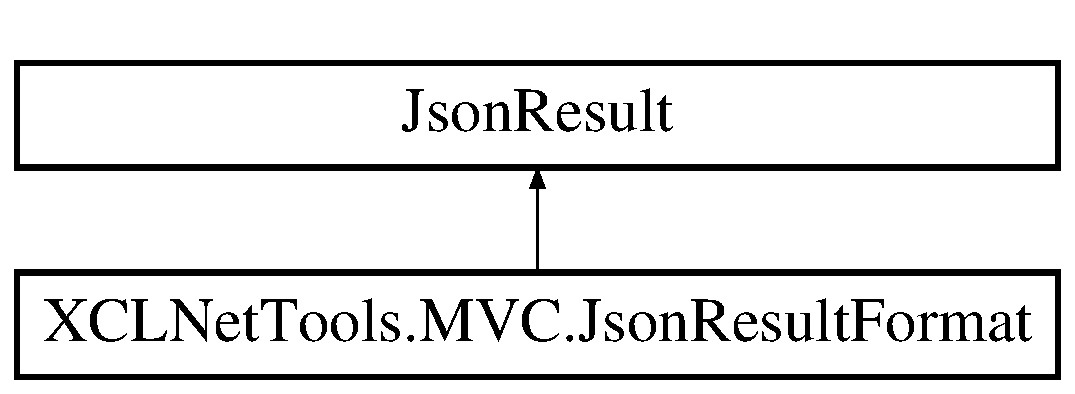
\includegraphics[height=2.000000cm]{class_x_c_l_net_tools_1_1_m_v_c_1_1_json_result_format}
\end{center}
\end{figure}
\subsection*{Public 成员函数}
\begin{DoxyCompactItemize}
\item 
override void \hyperlink{class_x_c_l_net_tools_1_1_m_v_c_1_1_json_result_format_aa8f3283c42c9130afd1aa8990876f413}{Execute\-Result} (Controller\-Context context)
\begin{DoxyCompactList}\small\item\em 重写执行视图 \end{DoxyCompactList}\end{DoxyCompactItemize}
\subsection*{属性}
\begin{DoxyCompactItemize}
\item 
string \hyperlink{class_x_c_l_net_tools_1_1_m_v_c_1_1_json_result_format_afc01b7cf2cd3f17c481c25ad70fcd4f6}{Date\-Format}\hspace{0.3cm}{\ttfamily  \mbox{[}get, set\mbox{]}}
\begin{DoxyCompactList}\small\item\em 格式化时间,默认值为\char`\"{}yyyy-\/\-M\-M-\/dd H\-H\-:mm\-:ss\char`\"{} \end{DoxyCompactList}\end{DoxyCompactItemize}


\subsection{详细描述}
带时间格式的json\-Result 



在文件 Json\-Result\-Format.\-cs 第 19 行定义.



\subsection{成员函数说明}
\hypertarget{class_x_c_l_net_tools_1_1_m_v_c_1_1_json_result_format_aa8f3283c42c9130afd1aa8990876f413}{\index{X\-C\-L\-Net\-Tools\-::\-M\-V\-C\-::\-Json\-Result\-Format@{X\-C\-L\-Net\-Tools\-::\-M\-V\-C\-::\-Json\-Result\-Format}!Execute\-Result@{Execute\-Result}}
\index{Execute\-Result@{Execute\-Result}!XCLNetTools::MVC::JsonResultFormat@{X\-C\-L\-Net\-Tools\-::\-M\-V\-C\-::\-Json\-Result\-Format}}
\subsubsection[{Execute\-Result}]{\setlength{\rightskip}{0pt plus 5cm}override void X\-C\-L\-Net\-Tools.\-M\-V\-C.\-Json\-Result\-Format.\-Execute\-Result (
\begin{DoxyParamCaption}
\item[{Controller\-Context}]{context}
\end{DoxyParamCaption}
)}}\label{class_x_c_l_net_tools_1_1_m_v_c_1_1_json_result_format_aa8f3283c42c9130afd1aa8990876f413}


重写执行视图 


\begin{DoxyParams}{参数}
{\em context} & 上下文\\
\hline
\end{DoxyParams}


在文件 Json\-Result\-Format.\-cs 第 36 行定义.



\subsection{属性说明}
\hypertarget{class_x_c_l_net_tools_1_1_m_v_c_1_1_json_result_format_afc01b7cf2cd3f17c481c25ad70fcd4f6}{\index{X\-C\-L\-Net\-Tools\-::\-M\-V\-C\-::\-Json\-Result\-Format@{X\-C\-L\-Net\-Tools\-::\-M\-V\-C\-::\-Json\-Result\-Format}!Date\-Format@{Date\-Format}}
\index{Date\-Format@{Date\-Format}!XCLNetTools::MVC::JsonResultFormat@{X\-C\-L\-Net\-Tools\-::\-M\-V\-C\-::\-Json\-Result\-Format}}
\subsubsection[{Date\-Format}]{\setlength{\rightskip}{0pt plus 5cm}string X\-C\-L\-Net\-Tools.\-M\-V\-C.\-Json\-Result\-Format.\-Date\-Format\hspace{0.3cm}{\ttfamily [get]}, {\ttfamily [set]}}}\label{class_x_c_l_net_tools_1_1_m_v_c_1_1_json_result_format_afc01b7cf2cd3f17c481c25ad70fcd4f6}


格式化时间,默认值为\char`\"{}yyyy-\/\-M\-M-\/dd H\-H\-:mm\-:ss\char`\"{} 



在文件 Json\-Result\-Format.\-cs 第 27 行定义.



该类的文档由以下文件生成\-:\begin{DoxyCompactItemize}
\item 
D\-:/\-My\-Data/\-My\-Git/\-Git\-Hub/\-X\-C\-L\-Net\-Tools/\-X\-C\-L\-Net\-Tools/\-M\-V\-C/\hyperlink{_json_result_format_8cs}{Json\-Result\-Format.\-cs}\end{DoxyCompactItemize}

\hypertarget{class_x_c_l_net_tools_1_1_entity_1_1_key_value}{}\section{X\+C\+L\+Net\+Tools.\+Entity.\+Key\+Value类 参考}
\label{class_x_c_l_net_tools_1_1_entity_1_1_key_value}\index{X\+C\+L\+Net\+Tools.\+Entity.\+Key\+Value@{X\+C\+L\+Net\+Tools.\+Entity.\+Key\+Value}}


键值类  


\subsection*{属性}
\begin{DoxyCompactItemize}
\item 
string \hyperlink{class_x_c_l_net_tools_1_1_entity_1_1_key_value_a33e2f7bfdcc6a1dce560304a4450cf08}{Key}\hspace{0.3cm}{\ttfamily  \mbox{[}get, set\mbox{]}}
\begin{DoxyCompactList}\small\item\em 键 \end{DoxyCompactList}\item 
string \hyperlink{class_x_c_l_net_tools_1_1_entity_1_1_key_value_a9ec3c76143930f64c1e0de2074514bae}{Value}\hspace{0.3cm}{\ttfamily  \mbox{[}get, set\mbox{]}}
\begin{DoxyCompactList}\small\item\em 值 \end{DoxyCompactList}\end{DoxyCompactItemize}


\subsection{详细描述}
键值类 



在文件 Key\+Value.\+cs 第 17 行定义.



\subsection{属性说明}
\mbox{\Hypertarget{class_x_c_l_net_tools_1_1_entity_1_1_key_value_a33e2f7bfdcc6a1dce560304a4450cf08}\label{class_x_c_l_net_tools_1_1_entity_1_1_key_value_a33e2f7bfdcc6a1dce560304a4450cf08}} 
\index{X\+C\+L\+Net\+Tools\+::\+Entity\+::\+Key\+Value@{X\+C\+L\+Net\+Tools\+::\+Entity\+::\+Key\+Value}!Key@{Key}}
\index{Key@{Key}!X\+C\+L\+Net\+Tools\+::\+Entity\+::\+Key\+Value@{X\+C\+L\+Net\+Tools\+::\+Entity\+::\+Key\+Value}}
\subsubsection{\texorpdfstring{Key}{Key}}
{\footnotesize\ttfamily string X\+C\+L\+Net\+Tools.\+Entity.\+Key\+Value.\+Key\hspace{0.3cm}{\ttfamily [get]}, {\ttfamily [set]}}



键 



在文件 Key\+Value.\+cs 第 22 行定义.

\mbox{\Hypertarget{class_x_c_l_net_tools_1_1_entity_1_1_key_value_a9ec3c76143930f64c1e0de2074514bae}\label{class_x_c_l_net_tools_1_1_entity_1_1_key_value_a9ec3c76143930f64c1e0de2074514bae}} 
\index{X\+C\+L\+Net\+Tools\+::\+Entity\+::\+Key\+Value@{X\+C\+L\+Net\+Tools\+::\+Entity\+::\+Key\+Value}!Value@{Value}}
\index{Value@{Value}!X\+C\+L\+Net\+Tools\+::\+Entity\+::\+Key\+Value@{X\+C\+L\+Net\+Tools\+::\+Entity\+::\+Key\+Value}}
\subsubsection{\texorpdfstring{Value}{Value}}
{\footnotesize\ttfamily string X\+C\+L\+Net\+Tools.\+Entity.\+Key\+Value.\+Value\hspace{0.3cm}{\ttfamily [get]}, {\ttfamily [set]}}



值 



在文件 Key\+Value.\+cs 第 27 行定义.



该类的文档由以下文件生成\+:\begin{DoxyCompactItemize}
\item 
D\+:/\+My\+Data/\+Git\+Hub/\+X\+C\+L\+Net\+Tools/\+X\+C\+L\+Net\+Tools/\+Entity/\hyperlink{_key_value_8cs}{Key\+Value.\+cs}\end{DoxyCompactItemize}

\hypertarget{class_x_c_l_net_tools_1_1_control_1_1_server_control_1_1_lib}{}\section{X\+C\+L\+Net\+Tools.\+Control.\+Server\+Control.\+Lib类 参考}
\label{class_x_c_l_net_tools_1_1_control_1_1_server_control_1_1_lib}\index{X\+C\+L\+Net\+Tools.\+Control.\+Server\+Control.\+Lib@{X\+C\+L\+Net\+Tools.\+Control.\+Server\+Control.\+Lib}}


服务器控件操作相关  


\subsection*{静态 Public 成员函数}
\begin{DoxyCompactItemize}
\item 
static void \hyperlink{class_x_c_l_net_tools_1_1_control_1_1_server_control_1_1_lib_a788673e8352bff030ce50d1b42cfd44f}{Rep\+Data\+Bind$<$ T $>$} (Repeater rep, List$<$ T $>$ data\+Source, bool is\+Show\+No\+Data\+Msg, params string\mbox{[}$\,$\mbox{]} no\+Data\+Msg)
\begin{DoxyCompactList}\small\item\em Repeater绑定数据 \end{DoxyCompactList}\item 
static void \hyperlink{class_x_c_l_net_tools_1_1_control_1_1_server_control_1_1_lib_ad2856902e5c392c722a55c82d9977586}{Rep\+Data\+Bind} (Repeater rep, Data\+Table data\+Source, bool is\+Show\+No\+Data\+Msg, params string\mbox{[}$\,$\mbox{]} no\+Data\+Msg)
\begin{DoxyCompactList}\small\item\em Repeater绑定数据 \end{DoxyCompactList}\item 
static void \hyperlink{class_x_c_l_net_tools_1_1_control_1_1_server_control_1_1_lib_a7d5141c14830a52c7d4edcab2d104452}{Bind\+D\+DL} (System.\+Web.\+U\+I.\+Web\+Controls.\+Drop\+Down\+List ddl, Data\+Set ds, string text\+Field, string value\+Field, string value, bool flag)
\begin{DoxyCompactList}\small\item\em 绑定\+D\+D\+L,value为初始选中值 \end{DoxyCompactList}\item 
static void \hyperlink{class_x_c_l_net_tools_1_1_control_1_1_server_control_1_1_lib_af2a5dcd9fa457696d15a072e4772b861}{Bind\+Check\+Box\+List} (System.\+Web.\+U\+I.\+Web\+Controls.\+Check\+Box\+List ck, Data\+Set ds, string text\+Field, string value\+Field, string value)
\begin{DoxyCompactList}\small\item\em 绑定\+Check\+Box\+List,value为初始选中值 \end{DoxyCompactList}\item 
static void \hyperlink{class_x_c_l_net_tools_1_1_control_1_1_server_control_1_1_lib_acf0e494ba2e94742818fbebfd883ab17}{Bind\+Enum} (System.\+Web.\+U\+I.\+Web\+Controls.\+Web\+Control c, List$<$ \hyperlink{class_x_c_l_net_tools_1_1_entity_1_1_text_value}{X\+C\+L\+Net\+Tools.\+Entity.\+Text\+Value} $>$ lst, string default\+Value)
\begin{DoxyCompactList}\small\item\em 绑定枚举(此方法已过期,请使用\+Bind\+Lst) \end{DoxyCompactList}\item 
static void \hyperlink{class_x_c_l_net_tools_1_1_control_1_1_server_control_1_1_lib_ad5ebfd4eb97120e0049cd0260e150ed9}{Bind\+Lst$<$ T $>$} (System.\+Web.\+U\+I.\+Web\+Controls.\+Web\+Control c, List$<$ T $>$ lst, string text\+Field, string value\+Field, string value, bool flag)
\begin{DoxyCompactList}\small\item\em 将list绑定到控件上 \end{DoxyCompactList}\end{DoxyCompactItemize}


\subsection{详细描述}
服务器控件操作相关 



在文件 Lib.\+cs 第 19 行定义.



\subsection{成员函数说明}
\index{X\+C\+L\+Net\+Tools\+::\+Control\+::\+Server\+Control\+::\+Lib@{X\+C\+L\+Net\+Tools\+::\+Control\+::\+Server\+Control\+::\+Lib}!Bind\+Check\+Box\+List@{Bind\+Check\+Box\+List}}
\index{Bind\+Check\+Box\+List@{Bind\+Check\+Box\+List}!X\+C\+L\+Net\+Tools\+::\+Control\+::\+Server\+Control\+::\+Lib@{X\+C\+L\+Net\+Tools\+::\+Control\+::\+Server\+Control\+::\+Lib}}
\subsubsection[{\texorpdfstring{Bind\+Check\+Box\+List(\+System.\+Web.\+U\+I.\+Web\+Controls.\+Check\+Box\+List ck, Data\+Set ds, string text\+Field, string value\+Field, string value)}{BindCheckBoxList(System.Web.UI.WebControls.CheckBoxList ck, DataSet ds, string textField, string valueField, string value)}}]{\setlength{\rightskip}{0pt plus 5cm}static void X\+C\+L\+Net\+Tools.\+Control.\+Server\+Control.\+Lib.\+Bind\+Check\+Box\+List (
\begin{DoxyParamCaption}
\item[{System.\+Web.\+U\+I.\+Web\+Controls.\+Check\+Box\+List}]{ck, }
\item[{Data\+Set}]{ds, }
\item[{string}]{text\+Field, }
\item[{string}]{value\+Field, }
\item[{string}]{value}
\end{DoxyParamCaption}
)\hspace{0.3cm}{\ttfamily [static]}}\hypertarget{class_x_c_l_net_tools_1_1_control_1_1_server_control_1_1_lib_af2a5dcd9fa457696d15a072e4772b861}{}\label{class_x_c_l_net_tools_1_1_control_1_1_server_control_1_1_lib_af2a5dcd9fa457696d15a072e4772b861}


绑定\+Check\+Box\+List,value为初始选中值 


\begin{DoxyParams}{参数}
{\em ck} & Check\+Box\+List\\
\hline
{\em ds} & dataset\\
\hline
{\em text\+Field} & 文本字段\\
\hline
{\em value\+Field} & 值字段\\
\hline
{\em value} & 以,隔开的字符串,默认选中值\\
\hline
\end{DoxyParams}


在文件 Lib.\+cs 第 115 行定义.

\index{X\+C\+L\+Net\+Tools\+::\+Control\+::\+Server\+Control\+::\+Lib@{X\+C\+L\+Net\+Tools\+::\+Control\+::\+Server\+Control\+::\+Lib}!Bind\+D\+DL@{Bind\+D\+DL}}
\index{Bind\+D\+DL@{Bind\+D\+DL}!X\+C\+L\+Net\+Tools\+::\+Control\+::\+Server\+Control\+::\+Lib@{X\+C\+L\+Net\+Tools\+::\+Control\+::\+Server\+Control\+::\+Lib}}
\subsubsection[{\texorpdfstring{Bind\+D\+D\+L(\+System.\+Web.\+U\+I.\+Web\+Controls.\+Drop\+Down\+List ddl, Data\+Set ds, string text\+Field, string value\+Field, string value, bool flag)}{BindDDL(System.Web.UI.WebControls.DropDownList ddl, DataSet ds, string textField, string valueField, string value, bool flag)}}]{\setlength{\rightskip}{0pt plus 5cm}static void X\+C\+L\+Net\+Tools.\+Control.\+Server\+Control.\+Lib.\+Bind\+D\+DL (
\begin{DoxyParamCaption}
\item[{System.\+Web.\+U\+I.\+Web\+Controls.\+Drop\+Down\+List}]{ddl, }
\item[{Data\+Set}]{ds, }
\item[{string}]{text\+Field, }
\item[{string}]{value\+Field, }
\item[{string}]{value, }
\item[{bool}]{flag}
\end{DoxyParamCaption}
)\hspace{0.3cm}{\ttfamily [static]}}\hypertarget{class_x_c_l_net_tools_1_1_control_1_1_server_control_1_1_lib_a7d5141c14830a52c7d4edcab2d104452}{}\label{class_x_c_l_net_tools_1_1_control_1_1_server_control_1_1_lib_a7d5141c14830a52c7d4edcab2d104452}


绑定\+D\+D\+L,value为初始选中值 


\begin{DoxyParams}{参数}
{\em ddl} & Drop\+Down\+List\\
\hline
{\em ds} & dataset\\
\hline
{\em text\+Field} & 文本字段\\
\hline
{\em value\+Field} & 值字段\\
\hline
{\em value} & 默认选中项的值\\
\hline
{\em flag} & true\+:有\char`\"{}-\/-\/全部-\/-\/\char`\"{} false\+:无\\
\hline
\end{DoxyParams}


在文件 Lib.\+cs 第 84 行定义.

\index{X\+C\+L\+Net\+Tools\+::\+Control\+::\+Server\+Control\+::\+Lib@{X\+C\+L\+Net\+Tools\+::\+Control\+::\+Server\+Control\+::\+Lib}!Bind\+Enum@{Bind\+Enum}}
\index{Bind\+Enum@{Bind\+Enum}!X\+C\+L\+Net\+Tools\+::\+Control\+::\+Server\+Control\+::\+Lib@{X\+C\+L\+Net\+Tools\+::\+Control\+::\+Server\+Control\+::\+Lib}}
\subsubsection[{\texorpdfstring{Bind\+Enum(\+System.\+Web.\+U\+I.\+Web\+Controls.\+Web\+Control c, List$<$ X\+C\+L\+Net\+Tools.\+Entity.\+Text\+Value $>$ lst, string default\+Value)}{BindEnum(System.Web.UI.WebControls.WebControl c, List< XCLNetTools.Entity.TextValue > lst, string defaultValue)}}]{\setlength{\rightskip}{0pt plus 5cm}static void X\+C\+L\+Net\+Tools.\+Control.\+Server\+Control.\+Lib.\+Bind\+Enum (
\begin{DoxyParamCaption}
\item[{System.\+Web.\+U\+I.\+Web\+Controls.\+Web\+Control}]{c, }
\item[{List$<$ {\bf X\+C\+L\+Net\+Tools.\+Entity.\+Text\+Value} $>$}]{lst, }
\item[{string}]{default\+Value}
\end{DoxyParamCaption}
)\hspace{0.3cm}{\ttfamily [static]}}\hypertarget{class_x_c_l_net_tools_1_1_control_1_1_server_control_1_1_lib_acf0e494ba2e94742818fbebfd883ab17}{}\label{class_x_c_l_net_tools_1_1_control_1_1_server_control_1_1_lib_acf0e494ba2e94742818fbebfd883ab17}


绑定枚举(此方法已过期,请使用\+Bind\+Lst) 


\begin{DoxyParams}{参数}
{\em c} & 控件\\
\hline
{\em lst} & \hyperlink{class_x_c_l_net_tools_1_1_entity_1_1_text_value}{X\+C\+L\+Net\+Tools.\+Entity.\+Text\+Value} list\\
\hline
{\em default\+Value} & 默认选中值\\
\hline
\end{DoxyParams}


在文件 Lib.\+cs 第 152 行定义.

\index{X\+C\+L\+Net\+Tools\+::\+Control\+::\+Server\+Control\+::\+Lib@{X\+C\+L\+Net\+Tools\+::\+Control\+::\+Server\+Control\+::\+Lib}!Bind\+Lst$<$ T $>$@{Bind\+Lst$<$ T $>$}}
\index{Bind\+Lst$<$ T $>$@{Bind\+Lst$<$ T $>$}!X\+C\+L\+Net\+Tools\+::\+Control\+::\+Server\+Control\+::\+Lib@{X\+C\+L\+Net\+Tools\+::\+Control\+::\+Server\+Control\+::\+Lib}}
\subsubsection[{\texorpdfstring{Bind\+Lst$<$ T $>$(\+System.\+Web.\+U\+I.\+Web\+Controls.\+Web\+Control c, List$<$ T $>$ lst, string text\+Field, string value\+Field, string value, bool flag)}{BindLst< T >(System.Web.UI.WebControls.WebControl c, List< T > lst, string textField, string valueField, string value, bool flag)}}]{\setlength{\rightskip}{0pt plus 5cm}static void X\+C\+L\+Net\+Tools.\+Control.\+Server\+Control.\+Lib.\+Bind\+Lst$<$ T $>$ (
\begin{DoxyParamCaption}
\item[{System.\+Web.\+U\+I.\+Web\+Controls.\+Web\+Control}]{c, }
\item[{List$<$ T $>$}]{lst, }
\item[{string}]{text\+Field, }
\item[{string}]{value\+Field, }
\item[{string}]{value, }
\item[{bool}]{flag}
\end{DoxyParamCaption}
)\hspace{0.3cm}{\ttfamily [static]}}\hypertarget{class_x_c_l_net_tools_1_1_control_1_1_server_control_1_1_lib_ad5ebfd4eb97120e0049cd0260e150ed9}{}\label{class_x_c_l_net_tools_1_1_control_1_1_server_control_1_1_lib_ad5ebfd4eb97120e0049cd0260e150ed9}


将list绑定到控件上 


\begin{DoxyParams}{参数}
{\em c} & 控件\\
\hline
{\em lst} & 数据源\\
\hline
{\em text\+Field} & 文本字段\\
\hline
{\em value\+Field} & 值字段\\
\hline
{\em value} & 选中值\\
\hline
{\em flag} & 第一项是否为\char`\"{}请选择\char`\"{}\\
\hline
\end{DoxyParams}


在文件 Lib.\+cs 第 180 行定义.

\index{X\+C\+L\+Net\+Tools\+::\+Control\+::\+Server\+Control\+::\+Lib@{X\+C\+L\+Net\+Tools\+::\+Control\+::\+Server\+Control\+::\+Lib}!Rep\+Data\+Bind@{Rep\+Data\+Bind}}
\index{Rep\+Data\+Bind@{Rep\+Data\+Bind}!X\+C\+L\+Net\+Tools\+::\+Control\+::\+Server\+Control\+::\+Lib@{X\+C\+L\+Net\+Tools\+::\+Control\+::\+Server\+Control\+::\+Lib}}
\subsubsection[{\texorpdfstring{Rep\+Data\+Bind(\+Repeater rep, Data\+Table data\+Source, bool is\+Show\+No\+Data\+Msg, params string[] no\+Data\+Msg)}{RepDataBind(Repeater rep, DataTable dataSource, bool isShowNoDataMsg, params string[] noDataMsg)}}]{\setlength{\rightskip}{0pt plus 5cm}static void X\+C\+L\+Net\+Tools.\+Control.\+Server\+Control.\+Lib.\+Rep\+Data\+Bind (
\begin{DoxyParamCaption}
\item[{Repeater}]{rep, }
\item[{Data\+Table}]{data\+Source, }
\item[{bool}]{is\+Show\+No\+Data\+Msg, }
\item[{params string\mbox{[}$\,$\mbox{]}}]{no\+Data\+Msg}
\end{DoxyParamCaption}
)\hspace{0.3cm}{\ttfamily [static]}}\hypertarget{class_x_c_l_net_tools_1_1_control_1_1_server_control_1_1_lib_ad2856902e5c392c722a55c82d9977586}{}\label{class_x_c_l_net_tools_1_1_control_1_1_server_control_1_1_lib_ad2856902e5c392c722a55c82d9977586}


Repeater绑定数据 


\begin{DoxyParams}{参数}
{\em rep} & Repeater控件\\
\hline
{\em data\+Source} & 数据源\\
\hline
{\em is\+Show\+No\+Data\+Msg} & true\+:没有数据时,显示“暂无数据”\\
\hline
{\em no\+Data\+Msg} & 没有数据时非默认提示\\
\hline
\end{DoxyParams}


在文件 Lib.\+cs 第 54 行定义.

\index{X\+C\+L\+Net\+Tools\+::\+Control\+::\+Server\+Control\+::\+Lib@{X\+C\+L\+Net\+Tools\+::\+Control\+::\+Server\+Control\+::\+Lib}!Rep\+Data\+Bind$<$ T $>$@{Rep\+Data\+Bind$<$ T $>$}}
\index{Rep\+Data\+Bind$<$ T $>$@{Rep\+Data\+Bind$<$ T $>$}!X\+C\+L\+Net\+Tools\+::\+Control\+::\+Server\+Control\+::\+Lib@{X\+C\+L\+Net\+Tools\+::\+Control\+::\+Server\+Control\+::\+Lib}}
\subsubsection[{\texorpdfstring{Rep\+Data\+Bind$<$ T $>$(\+Repeater rep, List$<$ T $>$ data\+Source, bool is\+Show\+No\+Data\+Msg, params string[] no\+Data\+Msg)}{RepDataBind< T >(Repeater rep, List< T > dataSource, bool isShowNoDataMsg, params string[] noDataMsg)}}]{\setlength{\rightskip}{0pt plus 5cm}static void {\bf X\+C\+L\+Net\+Tools.\+Control.\+Server\+Control.\+Lib.\+Rep\+Data\+Bind}$<$ T $>$ (
\begin{DoxyParamCaption}
\item[{Repeater}]{rep, }
\item[{List$<$ T $>$}]{data\+Source, }
\item[{bool}]{is\+Show\+No\+Data\+Msg, }
\item[{params string\mbox{[}$\,$\mbox{]}}]{no\+Data\+Msg}
\end{DoxyParamCaption}
)\hspace{0.3cm}{\ttfamily [static]}}\hypertarget{class_x_c_l_net_tools_1_1_control_1_1_server_control_1_1_lib_a788673e8352bff030ce50d1b42cfd44f}{}\label{class_x_c_l_net_tools_1_1_control_1_1_server_control_1_1_lib_a788673e8352bff030ce50d1b42cfd44f}


Repeater绑定数据 


\begin{DoxyParams}{参数}
{\em rep} & Repeater控件\\
\hline
{\em data\+Source} & 数据源\\
\hline
{\em is\+Show\+No\+Data\+Msg} & true\+:没有数据时,显示“暂无数据”\\
\hline
{\em no\+Data\+Msg} & 没有数据时非默认提示\\
\hline
\end{DoxyParams}


在文件 Lib.\+cs 第 30 行定义.



该类的文档由以下文件生成\+:\begin{DoxyCompactItemize}
\item 
E\+:/\+Git\+Hub/\+X\+C\+L\+Net\+Tools/\+X\+C\+L\+Net\+Tools/\+Control/\+Server\+Control/\hyperlink{_control_2_server_control_2_lib_8cs}{Lib.\+cs}\end{DoxyCompactItemize}

\hypertarget{class_x_c_l_net_tools_1_1_control_1_1_mx_graph_1_1_lib}{}\section{X\+C\+L\+Net\+Tools.\+Control.\+Mx\+Graph.\+Lib类 参考}
\label{class_x_c_l_net_tools_1_1_control_1_1_mx_graph_1_1_lib}\index{X\+C\+L\+Net\+Tools.\+Control.\+Mx\+Graph.\+Lib@{X\+C\+L\+Net\+Tools.\+Control.\+Mx\+Graph.\+Lib}}


Mx\+Graph操作类  


\subsection*{静态 Public 成员函数}
\begin{DoxyCompactItemize}
\item 
static Image \hyperlink{class_x_c_l_net_tools_1_1_control_1_1_mx_graph_1_1_lib_abff455d51f61485d6bf26e0133af6000}{Get\+Image} (string xml)
\begin{DoxyCompactList}\small\item\em 根据view形式的xml生成图片 \end{DoxyCompactList}\item 
static void \hyperlink{class_x_c_l_net_tools_1_1_control_1_1_mx_graph_1_1_lib_ad6b09c60b11a1f51a6bf45cc3bde1b88}{Export\+Image} (string xml, string filename)
\begin{DoxyCompactList}\small\item\em 导出mx\+Graph为图片 \end{DoxyCompactList}\end{DoxyCompactItemize}


\subsection{详细描述}
Mx\+Graph操作类 



在文件 Lib.\+cs 第 22 行定义.



\subsection{成员函数说明}
\index{X\+C\+L\+Net\+Tools\+::\+Control\+::\+Mx\+Graph\+::\+Lib@{X\+C\+L\+Net\+Tools\+::\+Control\+::\+Mx\+Graph\+::\+Lib}!Export\+Image@{Export\+Image}}
\index{Export\+Image@{Export\+Image}!X\+C\+L\+Net\+Tools\+::\+Control\+::\+Mx\+Graph\+::\+Lib@{X\+C\+L\+Net\+Tools\+::\+Control\+::\+Mx\+Graph\+::\+Lib}}
\subsubsection[{\texorpdfstring{Export\+Image(string xml, string filename)}{ExportImage(string xml, string filename)}}]{\setlength{\rightskip}{0pt plus 5cm}static void X\+C\+L\+Net\+Tools.\+Control.\+Mx\+Graph.\+Lib.\+Export\+Image (
\begin{DoxyParamCaption}
\item[{string}]{xml, }
\item[{string}]{filename}
\end{DoxyParamCaption}
)\hspace{0.3cm}{\ttfamily [static]}}\hypertarget{class_x_c_l_net_tools_1_1_control_1_1_mx_graph_1_1_lib_ad6b09c60b11a1f51a6bf45cc3bde1b88}{}\label{class_x_c_l_net_tools_1_1_control_1_1_mx_graph_1_1_lib_ad6b09c60b11a1f51a6bf45cc3bde1b88}


导出mx\+Graph为图片 


\begin{DoxyParams}{参数}
{\em xml} & mx\+Graph的model的view形式的xml\\
\hline
{\em filename} & 导出后的文件名(包含扩展名)\\
\hline
\end{DoxyParams}


在文件 Lib.\+cs 第 45 行定义.

\index{X\+C\+L\+Net\+Tools\+::\+Control\+::\+Mx\+Graph\+::\+Lib@{X\+C\+L\+Net\+Tools\+::\+Control\+::\+Mx\+Graph\+::\+Lib}!Get\+Image@{Get\+Image}}
\index{Get\+Image@{Get\+Image}!X\+C\+L\+Net\+Tools\+::\+Control\+::\+Mx\+Graph\+::\+Lib@{X\+C\+L\+Net\+Tools\+::\+Control\+::\+Mx\+Graph\+::\+Lib}}
\subsubsection[{\texorpdfstring{Get\+Image(string xml)}{GetImage(string xml)}}]{\setlength{\rightskip}{0pt plus 5cm}static Image X\+C\+L\+Net\+Tools.\+Control.\+Mx\+Graph.\+Lib.\+Get\+Image (
\begin{DoxyParamCaption}
\item[{string}]{xml}
\end{DoxyParamCaption}
)\hspace{0.3cm}{\ttfamily [static]}}\hypertarget{class_x_c_l_net_tools_1_1_control_1_1_mx_graph_1_1_lib_abff455d51f61485d6bf26e0133af6000}{}\label{class_x_c_l_net_tools_1_1_control_1_1_mx_graph_1_1_lib_abff455d51f61485d6bf26e0133af6000}


根据view形式的xml生成图片 


\begin{DoxyParams}{参数}
{\em xml} & view形式的xml\\
\hline
\end{DoxyParams}
\begin{DoxyReturn}{返回}
image对象
\end{DoxyReturn}


在文件 Lib.\+cs 第 29 行定义.



该类的文档由以下文件生成\+:\begin{DoxyCompactItemize}
\item 
E\+:/\+Git\+Hub/\+X\+C\+L\+Net\+Tools/\+X\+C\+L\+Net\+Tools/\+Control/\+Mx\+Graph/\hyperlink{_control_2_mx_graph_2_lib_8cs}{Lib.\+cs}\end{DoxyCompactItemize}

\hypertarget{class_x_c_l_net_tools_1_1_control_1_1_html_control_1_1_lib}{\section{X\-C\-L\-Net\-Tools.\-Control.\-Html\-Control.\-Lib类 参考}
\label{class_x_c_l_net_tools_1_1_control_1_1_html_control_1_1_lib}\index{X\-C\-L\-Net\-Tools.\-Control.\-Html\-Control.\-Lib@{X\-C\-L\-Net\-Tools.\-Control.\-Html\-Control.\-Lib}}
}


原生html控件操作类  


\subsection*{静态 Public 成员函数}
\begin{DoxyCompactItemize}
\item 
static string \hyperlink{class_x_c_l_net_tools_1_1_control_1_1_html_control_1_1_lib_a6bc535ff27a3e67b2c4dac1d5e99aa8c}{Get\-Options} (Type t, \hyperlink{class_x_c_l_net_tools_1_1_entity_1_1_set_option_entity}{Set\-Option\-Entity} options=null)
\begin{DoxyCompactList}\small\item\em 将枚举转为select的options 
\begin{DoxyParams}{参数}
{\em t} & 枚举type\\
\hline
{\em options} & 选项\\
\hline
\end{DoxyParams}
\begin{DoxyReturn}{返回}
option字符串
\end{DoxyReturn}
\end{DoxyCompactList}\item 
static string \hyperlink{class_x_c_l_net_tools_1_1_control_1_1_html_control_1_1_lib_aea5ab0601c97a418ef6291f75aa7baff}{Get\-Options} (Dictionary$<$ string, string $>$ data\-Source, \hyperlink{class_x_c_l_net_tools_1_1_entity_1_1_set_option_entity}{Set\-Option\-Entity} options=null)
\begin{DoxyCompactList}\small\item\em 将\-Dictionary转为select 的options 注:option的text为字典的key,value为字典的value \end{DoxyCompactList}\item 
static string \hyperlink{class_x_c_l_net_tools_1_1_control_1_1_html_control_1_1_lib_a48013321b30150acdbf3fcf28955980e}{Get\-Options$<$ T\-Key, T\-Value $>$} (Dictionary$<$ T\-Key, T\-Value $>$ data\-Source, \hyperlink{class_x_c_l_net_tools_1_1_entity_1_1_set_option_entity}{Set\-Option\-Entity} options=null)
\begin{DoxyCompactList}\small\item\em 将\-Dictionary转为select 的options 注:option的text为字典的key,value为字典的value \end{DoxyCompactList}\end{DoxyCompactItemize}


\subsection{详细描述}
原生html控件操作类 



在文件 Lib.\-cs 第 19 行定义.



\subsection{成员函数说明}
\hypertarget{class_x_c_l_net_tools_1_1_control_1_1_html_control_1_1_lib_a6bc535ff27a3e67b2c4dac1d5e99aa8c}{\index{X\-C\-L\-Net\-Tools\-::\-Control\-::\-Html\-Control\-::\-Lib@{X\-C\-L\-Net\-Tools\-::\-Control\-::\-Html\-Control\-::\-Lib}!Get\-Options@{Get\-Options}}
\index{Get\-Options@{Get\-Options}!XCLNetTools::Control::HtmlControl::Lib@{X\-C\-L\-Net\-Tools\-::\-Control\-::\-Html\-Control\-::\-Lib}}
\subsubsection[{Get\-Options}]{\setlength{\rightskip}{0pt plus 5cm}static string X\-C\-L\-Net\-Tools.\-Control.\-Html\-Control.\-Lib.\-Get\-Options (
\begin{DoxyParamCaption}
\item[{Type}]{t, }
\item[{{\bf Set\-Option\-Entity}}]{options = {\ttfamily null}}
\end{DoxyParamCaption}
)\hspace{0.3cm}{\ttfamily [static]}}}\label{class_x_c_l_net_tools_1_1_control_1_1_html_control_1_1_lib_a6bc535ff27a3e67b2c4dac1d5e99aa8c}


将枚举转为select的options 
\begin{DoxyParams}{参数}
{\em t} & 枚举type\\
\hline
{\em options} & 选项\\
\hline
\end{DoxyParams}
\begin{DoxyReturn}{返回}
option字符串
\end{DoxyReturn}




在文件 Lib.\-cs 第 27 行定义.

\hypertarget{class_x_c_l_net_tools_1_1_control_1_1_html_control_1_1_lib_aea5ab0601c97a418ef6291f75aa7baff}{\index{X\-C\-L\-Net\-Tools\-::\-Control\-::\-Html\-Control\-::\-Lib@{X\-C\-L\-Net\-Tools\-::\-Control\-::\-Html\-Control\-::\-Lib}!Get\-Options@{Get\-Options}}
\index{Get\-Options@{Get\-Options}!XCLNetTools::Control::HtmlControl::Lib@{X\-C\-L\-Net\-Tools\-::\-Control\-::\-Html\-Control\-::\-Lib}}
\subsubsection[{Get\-Options}]{\setlength{\rightskip}{0pt plus 5cm}static string X\-C\-L\-Net\-Tools.\-Control.\-Html\-Control.\-Lib.\-Get\-Options (
\begin{DoxyParamCaption}
\item[{Dictionary$<$ string, string $>$}]{data\-Source, }
\item[{{\bf Set\-Option\-Entity}}]{options = {\ttfamily null}}
\end{DoxyParamCaption}
)\hspace{0.3cm}{\ttfamily [static]}}}\label{class_x_c_l_net_tools_1_1_control_1_1_html_control_1_1_lib_aea5ab0601c97a418ef6291f75aa7baff}


将\-Dictionary转为select 的options 注:option的text为字典的key,value为字典的value 


\begin{DoxyParams}{参数}
{\em data\-Source} & 数据源\\
\hline
{\em options} & 选项\\
\hline
\end{DoxyParams}
\begin{DoxyReturn}{返回}
option字符串
\end{DoxyReturn}


在文件 Lib.\-cs 第 107 行定义.

\hypertarget{class_x_c_l_net_tools_1_1_control_1_1_html_control_1_1_lib_a48013321b30150acdbf3fcf28955980e}{\index{X\-C\-L\-Net\-Tools\-::\-Control\-::\-Html\-Control\-::\-Lib@{X\-C\-L\-Net\-Tools\-::\-Control\-::\-Html\-Control\-::\-Lib}!Get\-Options$<$ T\-Key, T\-Value $>$@{Get\-Options$<$ T\-Key, T\-Value $>$}}
\index{Get\-Options$<$ T\-Key, T\-Value $>$@{Get\-Options$<$ T\-Key, T\-Value $>$}!XCLNetTools::Control::HtmlControl::Lib@{X\-C\-L\-Net\-Tools\-::\-Control\-::\-Html\-Control\-::\-Lib}}
\subsubsection[{Get\-Options$<$ T\-Key, T\-Value $>$}]{\setlength{\rightskip}{0pt plus 5cm}static string {\bf X\-C\-L\-Net\-Tools.\-Control.\-Html\-Control.\-Lib.\-Get\-Options}$<$ T\-Key, T\-Value $>$ (
\begin{DoxyParamCaption}
\item[{Dictionary$<$ T\-Key, T\-Value $>$}]{data\-Source, }
\item[{{\bf Set\-Option\-Entity}}]{options = {\ttfamily null}}
\end{DoxyParamCaption}
)\hspace{0.3cm}{\ttfamily [static]}}}\label{class_x_c_l_net_tools_1_1_control_1_1_html_control_1_1_lib_a48013321b30150acdbf3fcf28955980e}


将\-Dictionary转为select 的options 注:option的text为字典的key,value为字典的value 


\begin{DoxyParams}{参数}
{\em data\-Source} & 数据源\\
\hline
{\em options} & 选项\\
\hline
\end{DoxyParams}
\begin{DoxyReturn}{返回}
option字符串
\end{DoxyReturn}


在文件 Lib.\-cs 第 138 行定义.



该类的文档由以下文件生成\-:\begin{DoxyCompactItemize}
\item 
D\-:/\-My\-Data/\-My\-Git/\-Git\-Hub/\-X\-C\-L\-Net\-Tools/\-X\-C\-L\-Net\-Tools/\-Control/\-Html\-Control/\hyperlink{_control_2_html_control_2_lib_8cs}{Lib.\-cs}\end{DoxyCompactItemize}

\hypertarget{class_x_c_l_net_tools_1_1_serialize_1_1_lib}{\section{X\-C\-L\-Net\-Tools.\-Serialize.\-Lib类 参考}
\label{class_x_c_l_net_tools_1_1_serialize_1_1_lib}\index{X\-C\-L\-Net\-Tools.\-Serialize.\-Lib@{X\-C\-L\-Net\-Tools.\-Serialize.\-Lib}}
}


其它对象序列化相关  


\subsection*{Public 成员函数}
\begin{DoxyCompactItemize}
\item 
T \hyperlink{class_x_c_l_net_tools_1_1_serialize_1_1_lib_ae2d400cea76a1f11f5141deab7c6d2b1}{Deserialize\-Object$<$ T $>$} (byte\mbox{[}$\,$\mbox{]} p\-Bytes)
\begin{DoxyCompactList}\small\item\em 把字节反序列化成相应的对象 \end{DoxyCompactList}\end{DoxyCompactItemize}
\subsection*{静态 Public 成员函数}
\begin{DoxyCompactItemize}
\item 
static T \hyperlink{class_x_c_l_net_tools_1_1_serialize_1_1_lib_ad38f60aaa57643027af6ebc86ef7fe18}{Deep\-Clone$<$ T $>$} (T source)
\begin{DoxyCompactList}\small\item\em 对象深度clone(被clone对象必须可以序列化) \end{DoxyCompactList}\item 
static Dictionary$<$ string, string $>$ \hyperlink{class_x_c_l_net_tools_1_1_serialize_1_1_lib_a99dccfb2469a4a61f20742a002a3f0ae}{Convert\-Json\-To\-Dictionary} (string json)
\begin{DoxyCompactList}\small\item\em 将\-J\-Object类型的属性转换为dictionary \end{DoxyCompactList}\item 
static string \hyperlink{class_x_c_l_net_tools_1_1_serialize_1_1_lib_a0034741d0598296a34082889f2a2f83e}{Convert\-Json\-To\-Url\-Parameters} (string json)
\begin{DoxyCompactList}\small\item\em 将\-J\-Object的属性转换为url参数形式 如:\{\char`\"{}a\char`\"{}\-:\char`\"{}1\char`\"{},\char`\"{}b\char`\"{}\-:\char`\"{}2\char`\"{},\char`\"{}c\char`\"{}\-:\{\char`\"{}d\char`\"{}\-:\char`\"{}100\char`\"{}\}\} -\/$>$ a=1\&b=2\&c.\-d=100 \end{DoxyCompactList}\end{DoxyCompactItemize}


\subsection{详细描述}
其它对象序列化相关 



在文件 Lib.\-cs 第 22 行定义.



\subsection{成员函数说明}
\hypertarget{class_x_c_l_net_tools_1_1_serialize_1_1_lib_a99dccfb2469a4a61f20742a002a3f0ae}{\index{X\-C\-L\-Net\-Tools\-::\-Serialize\-::\-Lib@{X\-C\-L\-Net\-Tools\-::\-Serialize\-::\-Lib}!Convert\-Json\-To\-Dictionary@{Convert\-Json\-To\-Dictionary}}
\index{Convert\-Json\-To\-Dictionary@{Convert\-Json\-To\-Dictionary}!XCLNetTools::Serialize::Lib@{X\-C\-L\-Net\-Tools\-::\-Serialize\-::\-Lib}}
\subsubsection[{Convert\-Json\-To\-Dictionary}]{\setlength{\rightskip}{0pt plus 5cm}static Dictionary$<$string, string$>$ X\-C\-L\-Net\-Tools.\-Serialize.\-Lib.\-Convert\-Json\-To\-Dictionary (
\begin{DoxyParamCaption}
\item[{string}]{json}
\end{DoxyParamCaption}
)\hspace{0.3cm}{\ttfamily [static]}}}\label{class_x_c_l_net_tools_1_1_serialize_1_1_lib_a99dccfb2469a4a61f20742a002a3f0ae}


将\-J\-Object类型的属性转换为dictionary 


\begin{DoxyParams}{参数}
{\em json} & 要转换的json\\
\hline
\end{DoxyParams}
\begin{DoxyReturn}{返回}
dictionary结果
\end{DoxyReturn}


在文件 Lib.\-cs 第 115 行定义.

\hypertarget{class_x_c_l_net_tools_1_1_serialize_1_1_lib_a0034741d0598296a34082889f2a2f83e}{\index{X\-C\-L\-Net\-Tools\-::\-Serialize\-::\-Lib@{X\-C\-L\-Net\-Tools\-::\-Serialize\-::\-Lib}!Convert\-Json\-To\-Url\-Parameters@{Convert\-Json\-To\-Url\-Parameters}}
\index{Convert\-Json\-To\-Url\-Parameters@{Convert\-Json\-To\-Url\-Parameters}!XCLNetTools::Serialize::Lib@{X\-C\-L\-Net\-Tools\-::\-Serialize\-::\-Lib}}
\subsubsection[{Convert\-Json\-To\-Url\-Parameters}]{\setlength{\rightskip}{0pt plus 5cm}static string X\-C\-L\-Net\-Tools.\-Serialize.\-Lib.\-Convert\-Json\-To\-Url\-Parameters (
\begin{DoxyParamCaption}
\item[{string}]{json}
\end{DoxyParamCaption}
)\hspace{0.3cm}{\ttfamily [static]}}}\label{class_x_c_l_net_tools_1_1_serialize_1_1_lib_a0034741d0598296a34082889f2a2f83e}


将\-J\-Object的属性转换为url参数形式 如:\{\char`\"{}a\char`\"{}\-:\char`\"{}1\char`\"{},\char`\"{}b\char`\"{}\-:\char`\"{}2\char`\"{},\char`\"{}c\char`\"{}\-:\{\char`\"{}d\char`\"{}\-:\char`\"{}100\char`\"{}\}\} -\/$>$ a=1\&b=2\&c.\-d=100 


\begin{DoxyParams}{参数}
{\em json} & 需要转换的json\\
\hline
\end{DoxyParams}
\begin{DoxyReturn}{返回}
url参数字符串
\end{DoxyReturn}


在文件 Lib.\-cs 第 136 行定义.

\hypertarget{class_x_c_l_net_tools_1_1_serialize_1_1_lib_ad38f60aaa57643027af6ebc86ef7fe18}{\index{X\-C\-L\-Net\-Tools\-::\-Serialize\-::\-Lib@{X\-C\-L\-Net\-Tools\-::\-Serialize\-::\-Lib}!Deep\-Clone$<$ T $>$@{Deep\-Clone$<$ T $>$}}
\index{Deep\-Clone$<$ T $>$@{Deep\-Clone$<$ T $>$}!XCLNetTools::Serialize::Lib@{X\-C\-L\-Net\-Tools\-::\-Serialize\-::\-Lib}}
\subsubsection[{Deep\-Clone$<$ T $>$}]{\setlength{\rightskip}{0pt plus 5cm}static T X\-C\-L\-Net\-Tools.\-Serialize.\-Lib.\-Deep\-Clone$<$ T $>$ (
\begin{DoxyParamCaption}
\item[{T}]{source}
\end{DoxyParamCaption}
)\hspace{0.3cm}{\ttfamily [static]}}}\label{class_x_c_l_net_tools_1_1_serialize_1_1_lib_ad38f60aaa57643027af6ebc86ef7fe18}


对象深度clone(被clone对象必须可以序列化) 


\begin{DoxyParams}{参数}
{\em source} & 要克隆的对象\\
\hline
\end{DoxyParams}
\begin{DoxyReturn}{返回}
克隆后的新对象
\end{DoxyReturn}
\begin{Desc}
\item[类型限制]\begin{description}
\item[{\em T} : {\em class}]\end{description}
\end{Desc}


在文件 Lib.\-cs 第 56 行定义.

\hypertarget{class_x_c_l_net_tools_1_1_serialize_1_1_lib_ae2d400cea76a1f11f5141deab7c6d2b1}{\index{X\-C\-L\-Net\-Tools\-::\-Serialize\-::\-Lib@{X\-C\-L\-Net\-Tools\-::\-Serialize\-::\-Lib}!Deserialize\-Object$<$ T $>$@{Deserialize\-Object$<$ T $>$}}
\index{Deserialize\-Object$<$ T $>$@{Deserialize\-Object$<$ T $>$}!XCLNetTools::Serialize::Lib@{X\-C\-L\-Net\-Tools\-::\-Serialize\-::\-Lib}}
\subsubsection[{Deserialize\-Object$<$ T $>$}]{\setlength{\rightskip}{0pt plus 5cm}T X\-C\-L\-Net\-Tools.\-Serialize.\-Lib.\-Deserialize\-Object$<$ T $>$ (
\begin{DoxyParamCaption}
\item[{byte\mbox{[}$\,$\mbox{]}}]{p\-Bytes}
\end{DoxyParamCaption}
)}}\label{class_x_c_l_net_tools_1_1_serialize_1_1_lib_ae2d400cea76a1f11f5141deab7c6d2b1}


把字节反序列化成相应的对象 


\begin{DoxyParams}{参数}
{\em p\-Bytes} & 字节流\\
\hline
\end{DoxyParams}
\begin{DoxyReturn}{返回}
T
\end{DoxyReturn}
\begin{Desc}
\item[类型限制]\begin{description}
\item[{\em T} : {\em class}]\end{description}
\end{Desc}


在文件 Lib.\-cs 第 31 行定义.



该类的文档由以下文件生成\-:\begin{DoxyCompactItemize}
\item 
D\-:/\-My\-Data/\-My\-Git/\-Git\-Hub/\-X\-C\-L\-Net\-Tools/\-X\-C\-L\-Net\-Tools/\-Serialize/\hyperlink{_serialize_2_lib_8cs}{Lib.\-cs}\end{DoxyCompactItemize}

\hypertarget{class_x_c_l_net_tools_1_1_encode_1_1_lib}{}\section{X\+C\+L\+Net\+Tools.\+Encode.\+Lib类 参考}
\label{class_x_c_l_net_tools_1_1_encode_1_1_lib}\index{X\+C\+L\+Net\+Tools.\+Encode.\+Lib@{X\+C\+L\+Net\+Tools.\+Encode.\+Lib}}


其它相关  


\subsection*{静态 Public 成员函数}
\begin{DoxyCompactItemize}
\item 
static string \hyperlink{class_x_c_l_net_tools_1_1_encode_1_1_lib_a3820bb303f5c96fa7e802f4cd0ac9ece}{Unescape} (string str)
\begin{DoxyCompactList}\small\item\em 对字符串进行js的unescape解码 \end{DoxyCompactList}\item 
static string \hyperlink{class_x_c_l_net_tools_1_1_encode_1_1_lib_aa5d0a56e854bbecc1fcdfea90f393600}{Escape} (string str)
\begin{DoxyCompactList}\small\item\em 对字符串进行js的escape编码 \end{DoxyCompactList}\end{DoxyCompactItemize}


\subsection{详细描述}
其它相关 



在文件 Lib.\+cs 第 14 行定义.



\subsection{成员函数说明}
\mbox{\Hypertarget{class_x_c_l_net_tools_1_1_encode_1_1_lib_aa5d0a56e854bbecc1fcdfea90f393600}\label{class_x_c_l_net_tools_1_1_encode_1_1_lib_aa5d0a56e854bbecc1fcdfea90f393600}} 
\index{X\+C\+L\+Net\+Tools\+::\+Encode\+::\+Lib@{X\+C\+L\+Net\+Tools\+::\+Encode\+::\+Lib}!Escape@{Escape}}
\index{Escape@{Escape}!X\+C\+L\+Net\+Tools\+::\+Encode\+::\+Lib@{X\+C\+L\+Net\+Tools\+::\+Encode\+::\+Lib}}
\subsubsection{\texorpdfstring{Escape()}{Escape()}}
{\footnotesize\ttfamily static string X\+C\+L\+Net\+Tools.\+Encode.\+Lib.\+Escape (\begin{DoxyParamCaption}\item[{string}]{str }\end{DoxyParamCaption})\hspace{0.3cm}{\ttfamily [static]}}



对字符串进行js的escape编码 


\begin{DoxyParams}{参数}
{\em str} & 待编码的字符串\\
\hline
\end{DoxyParams}
\begin{DoxyReturn}{返回}
编码后的值
\end{DoxyReturn}


在文件 Lib.\+cs 第 35 行定义.

\mbox{\Hypertarget{class_x_c_l_net_tools_1_1_encode_1_1_lib_a3820bb303f5c96fa7e802f4cd0ac9ece}\label{class_x_c_l_net_tools_1_1_encode_1_1_lib_a3820bb303f5c96fa7e802f4cd0ac9ece}} 
\index{X\+C\+L\+Net\+Tools\+::\+Encode\+::\+Lib@{X\+C\+L\+Net\+Tools\+::\+Encode\+::\+Lib}!Unescape@{Unescape}}
\index{Unescape@{Unescape}!X\+C\+L\+Net\+Tools\+::\+Encode\+::\+Lib@{X\+C\+L\+Net\+Tools\+::\+Encode\+::\+Lib}}
\subsubsection{\texorpdfstring{Unescape()}{Unescape()}}
{\footnotesize\ttfamily static string X\+C\+L\+Net\+Tools.\+Encode.\+Lib.\+Unescape (\begin{DoxyParamCaption}\item[{string}]{str }\end{DoxyParamCaption})\hspace{0.3cm}{\ttfamily [static]}}



对字符串进行js的unescape解码 


\begin{DoxyParams}{参数}
{\em str} & 待解码的字符串\\
\hline
\end{DoxyParams}
\begin{DoxyReturn}{返回}
解码后的值
\end{DoxyReturn}


在文件 Lib.\+cs 第 21 行定义.



该类的文档由以下文件生成\+:\begin{DoxyCompactItemize}
\item 
D\+:/\+My\+Data/\+Git\+Hub/\+X\+C\+L\+Net\+Tools/\+X\+C\+L\+Net\+Tools/\+Encode/\hyperlink{_encode_2_lib_8cs}{Lib.\+cs}\end{DoxyCompactItemize}

\hypertarget{class_x_c_l_net_tools_1_1_generic_1_1_list_helper}{\section{X\-C\-L\-Net\-Tools.\-Generic.\-List\-Helper类 参考}
\label{class_x_c_l_net_tools_1_1_generic_1_1_list_helper}\index{X\-C\-L\-Net\-Tools.\-Generic.\-List\-Helper@{X\-C\-L\-Net\-Tools.\-Generic.\-List\-Helper}}
}


List操作类  


\subsection*{静态 Public 成员函数}
\begin{DoxyCompactItemize}
\item 
static List$<$ List$<$ T $>$ $>$ \hyperlink{class_x_c_l_net_tools_1_1_generic_1_1_list_helper_a38adb871b8752fb797795645625b7b4f}{Split\-List\-By\-Step$<$ T $>$} (int step, List$<$ T $>$ lst)
\begin{DoxyCompactList}\small\item\em 根据步长,将一个总\-List拆分为多个子\-List \end{DoxyCompactList}\item 
static List$<$ string $>$ \hyperlink{class_x_c_l_net_tools_1_1_generic_1_1_list_helper_a3225ddcbde7d47ccef1ab295ebbd2f1d}{Get\-Str\-Split\-List} (string str, char speater)
\begin{DoxyCompactList}\small\item\em 将指定字符串用指定分隔符分开存到list中 \end{DoxyCompactList}\item 
static string \hyperlink{class_x_c_l_net_tools_1_1_generic_1_1_list_helper_a02b07a0f7a7d4506c358650ba010f7d9}{Get\-String\-By\-List$<$ T $>$} (List$<$ T $>$ lst, string split\-Char)
\begin{DoxyCompactList}\small\item\em 将list中的项拼接字符串 \end{DoxyCompactList}\item 
static Data\-Table \hyperlink{class_x_c_l_net_tools_1_1_generic_1_1_list_helper_aabb9427ae92df2eb55b7ea300be149a9}{To\-Data\-Table$<$ T $>$} (I\-List$<$ T $>$ data)
\begin{DoxyCompactList}\small\item\em 将\-List转换成\-Data\-Table \end{DoxyCompactList}\item 
static I\-List$<$ T $>$ \hyperlink{class_x_c_l_net_tools_1_1_generic_1_1_list_helper_aa1d5d2843b5a105edf4eb8c160fcd016}{Data\-Table\-To\-List$<$ T $>$} (Data\-Table dt)
\begin{DoxyCompactList}\small\item\em 将data\-Table转为list \end{DoxyCompactList}\end{DoxyCompactItemize}


\subsection{详细描述}
List操作类 



在文件 List\-Helper.\-cs 第 36 行定义.



\subsection{成员函数说明}
\hypertarget{class_x_c_l_net_tools_1_1_generic_1_1_list_helper_aa1d5d2843b5a105edf4eb8c160fcd016}{\index{X\-C\-L\-Net\-Tools\-::\-Generic\-::\-List\-Helper@{X\-C\-L\-Net\-Tools\-::\-Generic\-::\-List\-Helper}!Data\-Table\-To\-List$<$ T $>$@{Data\-Table\-To\-List$<$ T $>$}}
\index{Data\-Table\-To\-List$<$ T $>$@{Data\-Table\-To\-List$<$ T $>$}!XCLNetTools::Generic::ListHelper@{X\-C\-L\-Net\-Tools\-::\-Generic\-::\-List\-Helper}}
\subsubsection[{Data\-Table\-To\-List$<$ T $>$}]{\setlength{\rightskip}{0pt plus 5cm}static I\-List$<$T$>$ X\-C\-L\-Net\-Tools.\-Generic.\-List\-Helper.\-Data\-Table\-To\-List$<$ T $>$ (
\begin{DoxyParamCaption}
\item[{Data\-Table}]{dt}
\end{DoxyParamCaption}
)\hspace{0.3cm}{\ttfamily [static]}}}\label{class_x_c_l_net_tools_1_1_generic_1_1_list_helper_aa1d5d2843b5a105edf4eb8c160fcd016}


将data\-Table转为list 


\begin{DoxyParams}{参数}
{\em dt} & 要转换的数据\\
\hline
\end{DoxyParams}
\begin{DoxyReturn}{返回}
list
\end{DoxyReturn}
\begin{Desc}
\item[类型限制]\begin{description}
\item[{\em T} : {\em new()}]\end{description}
\end{Desc}


在文件 List\-Helper.\-cs 第 128 行定义.

\hypertarget{class_x_c_l_net_tools_1_1_generic_1_1_list_helper_a02b07a0f7a7d4506c358650ba010f7d9}{\index{X\-C\-L\-Net\-Tools\-::\-Generic\-::\-List\-Helper@{X\-C\-L\-Net\-Tools\-::\-Generic\-::\-List\-Helper}!Get\-String\-By\-List$<$ T $>$@{Get\-String\-By\-List$<$ T $>$}}
\index{Get\-String\-By\-List$<$ T $>$@{Get\-String\-By\-List$<$ T $>$}!XCLNetTools::Generic::ListHelper@{X\-C\-L\-Net\-Tools\-::\-Generic\-::\-List\-Helper}}
\subsubsection[{Get\-String\-By\-List$<$ T $>$}]{\setlength{\rightskip}{0pt plus 5cm}static string X\-C\-L\-Net\-Tools.\-Generic.\-List\-Helper.\-Get\-String\-By\-List$<$ T $>$ (
\begin{DoxyParamCaption}
\item[{List$<$ T $>$}]{lst, }
\item[{string}]{split\-Char}
\end{DoxyParamCaption}
)\hspace{0.3cm}{\ttfamily [static]}}}\label{class_x_c_l_net_tools_1_1_generic_1_1_list_helper_a02b07a0f7a7d4506c358650ba010f7d9}


将list中的项拼接字符串 


\begin{DoxyParams}{参数}
{\em lst} & 要操作的list\\
\hline
{\em split\-Char} & 分隔符\\
\hline
\end{DoxyParams}
\begin{DoxyReturn}{返回}
字符串结果值
\end{DoxyReturn}


在文件 List\-Helper.\-cs 第 87 行定义.

\hypertarget{class_x_c_l_net_tools_1_1_generic_1_1_list_helper_a3225ddcbde7d47ccef1ab295ebbd2f1d}{\index{X\-C\-L\-Net\-Tools\-::\-Generic\-::\-List\-Helper@{X\-C\-L\-Net\-Tools\-::\-Generic\-::\-List\-Helper}!Get\-Str\-Split\-List@{Get\-Str\-Split\-List}}
\index{Get\-Str\-Split\-List@{Get\-Str\-Split\-List}!XCLNetTools::Generic::ListHelper@{X\-C\-L\-Net\-Tools\-::\-Generic\-::\-List\-Helper}}
\subsubsection[{Get\-Str\-Split\-List}]{\setlength{\rightskip}{0pt plus 5cm}static List$<$string$>$ X\-C\-L\-Net\-Tools.\-Generic.\-List\-Helper.\-Get\-Str\-Split\-List (
\begin{DoxyParamCaption}
\item[{string}]{str, }
\item[{char}]{speater}
\end{DoxyParamCaption}
)\hspace{0.3cm}{\ttfamily [static]}}}\label{class_x_c_l_net_tools_1_1_generic_1_1_list_helper_a3225ddcbde7d47ccef1ab295ebbd2f1d}


将指定字符串用指定分隔符分开存到list中 


\begin{DoxyParams}{参数}
{\em str} & 源字符串\\
\hline
{\em speater} & 分隔字符\\
\hline
\end{DoxyParams}
\begin{DoxyReturn}{返回}
list
\end{DoxyReturn}


在文件 List\-Helper.\-cs 第 71 行定义.

\hypertarget{class_x_c_l_net_tools_1_1_generic_1_1_list_helper_a38adb871b8752fb797795645625b7b4f}{\index{X\-C\-L\-Net\-Tools\-::\-Generic\-::\-List\-Helper@{X\-C\-L\-Net\-Tools\-::\-Generic\-::\-List\-Helper}!Split\-List\-By\-Step$<$ T $>$@{Split\-List\-By\-Step$<$ T $>$}}
\index{Split\-List\-By\-Step$<$ T $>$@{Split\-List\-By\-Step$<$ T $>$}!XCLNetTools::Generic::ListHelper@{X\-C\-L\-Net\-Tools\-::\-Generic\-::\-List\-Helper}}
\subsubsection[{Split\-List\-By\-Step$<$ T $>$}]{\setlength{\rightskip}{0pt plus 5cm}static List$<$List$<$T$>$ $>$ X\-C\-L\-Net\-Tools.\-Generic.\-List\-Helper.\-Split\-List\-By\-Step$<$ T $>$ (
\begin{DoxyParamCaption}
\item[{int}]{step, }
\item[{List$<$ T $>$}]{lst}
\end{DoxyParamCaption}
)\hspace{0.3cm}{\ttfamily [static]}}}\label{class_x_c_l_net_tools_1_1_generic_1_1_list_helper_a38adb871b8752fb797795645625b7b4f}


根据步长,将一个总\-List拆分为多个子\-List 


\begin{DoxyParams}{参数}
{\em step} & 每个子list最多的项数\\
\hline
{\em lst} & 主list\\
\hline
\end{DoxyParams}
\begin{DoxyReturn}{返回}
分拆后的结果list
\end{DoxyReturn}


在文件 List\-Helper.\-cs 第 44 行定义.

\hypertarget{class_x_c_l_net_tools_1_1_generic_1_1_list_helper_aabb9427ae92df2eb55b7ea300be149a9}{\index{X\-C\-L\-Net\-Tools\-::\-Generic\-::\-List\-Helper@{X\-C\-L\-Net\-Tools\-::\-Generic\-::\-List\-Helper}!To\-Data\-Table$<$ T $>$@{To\-Data\-Table$<$ T $>$}}
\index{To\-Data\-Table$<$ T $>$@{To\-Data\-Table$<$ T $>$}!XCLNetTools::Generic::ListHelper@{X\-C\-L\-Net\-Tools\-::\-Generic\-::\-List\-Helper}}
\subsubsection[{To\-Data\-Table$<$ T $>$}]{\setlength{\rightskip}{0pt plus 5cm}static Data\-Table X\-C\-L\-Net\-Tools.\-Generic.\-List\-Helper.\-To\-Data\-Table$<$ T $>$ (
\begin{DoxyParamCaption}
\item[{I\-List$<$ T $>$}]{data}
\end{DoxyParamCaption}
)\hspace{0.3cm}{\ttfamily [static]}}}\label{class_x_c_l_net_tools_1_1_generic_1_1_list_helper_aabb9427ae92df2eb55b7ea300be149a9}


将\-List转换成\-Data\-Table 


\begin{DoxyParams}{参数}
{\em data} & 要转换的数据\\
\hline
\end{DoxyParams}
\begin{DoxyReturn}{返回}
datatable
\end{DoxyReturn}


在文件 List\-Helper.\-cs 第 102 行定义.



该类的文档由以下文件生成\-:\begin{DoxyCompactItemize}
\item 
D\-:/\-My\-Data/\-My\-Git/\-Git\-Hub/\-X\-C\-L\-Net\-Tools/\-X\-C\-L\-Net\-Tools/\-Generic/\hyperlink{_list_helper_8cs}{List\-Helper.\-cs}\end{DoxyCompactItemize}

\hypertarget{class_x_c_l_net_tools_1_1_serialize_1_1_lit_json}{}\section{X\+C\+L\+Net\+Tools.\+Serialize.\+Lit\+Json类 参考}
\label{class_x_c_l_net_tools_1_1_serialize_1_1_lit_json}\index{X\+C\+L\+Net\+Tools.\+Serialize.\+Lit\+Json@{X\+C\+L\+Net\+Tools.\+Serialize.\+Lit\+Json}}


Lit\+Json帮助类  


\subsection*{静态 Public 成员函数}
\begin{DoxyCompactItemize}
\item 
static string \hyperlink{class_x_c_l_net_tools_1_1_serialize_1_1_lit_json_a81a2b398d509a227753a98e12a79674e}{Convert\+Object\+To\+Json} (object obj)
\begin{DoxyCompactList}\small\item\em 对象转为json \end{DoxyCompactList}\item 
static string \hyperlink{class_x_c_l_net_tools_1_1_serialize_1_1_lit_json_a8bd51fdf8d1e56bee3e72c165f4d34ae}{Convert\+Data\+Table\+To\+Array} (System.\+Data.\+Data\+Table dt)
\begin{DoxyCompactList}\small\item\em Data\+Table转为js的数组形式,若为空,则返回\mbox{[}\mbox{]} \end{DoxyCompactList}\item 
static string \hyperlink{class_x_c_l_net_tools_1_1_serialize_1_1_lit_json_a118c20cd6f5a519aa5061f1d95f13c94}{Convert\+Data\+Table\+To\+Json} (Data\+Table dt, string json\+Name)
\begin{DoxyCompactList}\small\item\em Data\+Table转为json \end{DoxyCompactList}\item 
static string \hyperlink{class_x_c_l_net_tools_1_1_serialize_1_1_lit_json_a62018ecad0868724f8c525f6633c2db1}{Convert\+Data\+Set\+To\+Array} (System.\+Data.\+Data\+Set ds)
\begin{DoxyCompactList}\small\item\em Data\+Set转为js的数组形式,若为空,则返回\mbox{[}\mbox{]} \end{DoxyCompactList}\item 
static string \hyperlink{class_x_c_l_net_tools_1_1_serialize_1_1_lit_json_afe0e32c9376fb1c7f2c222eb8cfdcc18}{Convert\+Data\+Set\+To\+Json} (Data\+Set ds, string json\+Name)
\begin{DoxyCompactList}\small\item\em Data\+Set转为json \end{DoxyCompactList}\item 
static string \hyperlink{class_x_c_l_net_tools_1_1_serialize_1_1_lit_json_a97544159631e77ad1e2ab7fba119fce4}{Convert\+List\+To\+Json$<$ T $>$} (I\+List$<$ T $>$ lst, string json\+Name)
\begin{DoxyCompactList}\small\item\em List转为json \end{DoxyCompactList}\item 
static string \hyperlink{class_x_c_l_net_tools_1_1_serialize_1_1_lit_json_aed2848556cf9cdac6abfa0718a9a7fa4}{Convert\+List\+To\+Array$<$ T $>$} (I\+List$<$ T $>$ lst)
\begin{DoxyCompactList}\small\item\em List转为数组,若为空,则直接返回\mbox{[}\mbox{]} \end{DoxyCompactList}\end{DoxyCompactItemize}


\subsection{详细描述}
Lit\+Json帮助类 



在文件 Lit\+Json.\+cs 第 20 行定义.



\subsection{成员函数说明}
\index{X\+C\+L\+Net\+Tools\+::\+Serialize\+::\+Lit\+Json@{X\+C\+L\+Net\+Tools\+::\+Serialize\+::\+Lit\+Json}!Convert\+Data\+Set\+To\+Array@{Convert\+Data\+Set\+To\+Array}}
\index{Convert\+Data\+Set\+To\+Array@{Convert\+Data\+Set\+To\+Array}!X\+C\+L\+Net\+Tools\+::\+Serialize\+::\+Lit\+Json@{X\+C\+L\+Net\+Tools\+::\+Serialize\+::\+Lit\+Json}}
\subsubsection[{\texorpdfstring{Convert\+Data\+Set\+To\+Array(\+System.\+Data.\+Data\+Set ds)}{ConvertDataSetToArray(System.Data.DataSet ds)}}]{\setlength{\rightskip}{0pt plus 5cm}static string X\+C\+L\+Net\+Tools.\+Serialize.\+Lit\+Json.\+Convert\+Data\+Set\+To\+Array (
\begin{DoxyParamCaption}
\item[{System.\+Data.\+Data\+Set}]{ds}
\end{DoxyParamCaption}
)\hspace{0.3cm}{\ttfamily [static]}}\hypertarget{class_x_c_l_net_tools_1_1_serialize_1_1_lit_json_a62018ecad0868724f8c525f6633c2db1}{}\label{class_x_c_l_net_tools_1_1_serialize_1_1_lit_json_a62018ecad0868724f8c525f6633c2db1}


Data\+Set转为js的数组形式,若为空,则返回\mbox{[}\mbox{]} 


\begin{DoxyParams}{参数}
{\em ds} & 数据源\\
\hline
\end{DoxyParams}
\begin{DoxyReturn}{返回}
json数组
\end{DoxyReturn}


在文件 Lit\+Json.\+cs 第 88 行定义.

\index{X\+C\+L\+Net\+Tools\+::\+Serialize\+::\+Lit\+Json@{X\+C\+L\+Net\+Tools\+::\+Serialize\+::\+Lit\+Json}!Convert\+Data\+Set\+To\+Json@{Convert\+Data\+Set\+To\+Json}}
\index{Convert\+Data\+Set\+To\+Json@{Convert\+Data\+Set\+To\+Json}!X\+C\+L\+Net\+Tools\+::\+Serialize\+::\+Lit\+Json@{X\+C\+L\+Net\+Tools\+::\+Serialize\+::\+Lit\+Json}}
\subsubsection[{\texorpdfstring{Convert\+Data\+Set\+To\+Json(\+Data\+Set ds, string json\+Name)}{ConvertDataSetToJson(DataSet ds, string jsonName)}}]{\setlength{\rightskip}{0pt plus 5cm}static string X\+C\+L\+Net\+Tools.\+Serialize.\+Lit\+Json.\+Convert\+Data\+Set\+To\+Json (
\begin{DoxyParamCaption}
\item[{Data\+Set}]{ds, }
\item[{string}]{json\+Name}
\end{DoxyParamCaption}
)\hspace{0.3cm}{\ttfamily [static]}}\hypertarget{class_x_c_l_net_tools_1_1_serialize_1_1_lit_json_afe0e32c9376fb1c7f2c222eb8cfdcc18}{}\label{class_x_c_l_net_tools_1_1_serialize_1_1_lit_json_afe0e32c9376fb1c7f2c222eb8cfdcc18}


Data\+Set转为json 


\begin{DoxyParams}{参数}
{\em ds} & 数据源\\
\hline
{\em json\+Name} & 指定json key名\\
\hline
\end{DoxyParams}
\begin{DoxyReturn}{返回}
json
\end{DoxyReturn}


在文件 Lit\+Json.\+cs 第 109 行定义.

\index{X\+C\+L\+Net\+Tools\+::\+Serialize\+::\+Lit\+Json@{X\+C\+L\+Net\+Tools\+::\+Serialize\+::\+Lit\+Json}!Convert\+Data\+Table\+To\+Array@{Convert\+Data\+Table\+To\+Array}}
\index{Convert\+Data\+Table\+To\+Array@{Convert\+Data\+Table\+To\+Array}!X\+C\+L\+Net\+Tools\+::\+Serialize\+::\+Lit\+Json@{X\+C\+L\+Net\+Tools\+::\+Serialize\+::\+Lit\+Json}}
\subsubsection[{\texorpdfstring{Convert\+Data\+Table\+To\+Array(\+System.\+Data.\+Data\+Table dt)}{ConvertDataTableToArray(System.Data.DataTable dt)}}]{\setlength{\rightskip}{0pt plus 5cm}static string X\+C\+L\+Net\+Tools.\+Serialize.\+Lit\+Json.\+Convert\+Data\+Table\+To\+Array (
\begin{DoxyParamCaption}
\item[{System.\+Data.\+Data\+Table}]{dt}
\end{DoxyParamCaption}
)\hspace{0.3cm}{\ttfamily [static]}}\hypertarget{class_x_c_l_net_tools_1_1_serialize_1_1_lit_json_a8bd51fdf8d1e56bee3e72c165f4d34ae}{}\label{class_x_c_l_net_tools_1_1_serialize_1_1_lit_json_a8bd51fdf8d1e56bee3e72c165f4d34ae}


Data\+Table转为js的数组形式,若为空,则返回\mbox{[}\mbox{]} 


\begin{DoxyParams}{参数}
{\em dt} & 要处理的数据\\
\hline
\end{DoxyParams}
\begin{DoxyReturn}{返回}
json数组
\end{DoxyReturn}


在文件 Lit\+Json.\+cs 第 39 行定义.

\index{X\+C\+L\+Net\+Tools\+::\+Serialize\+::\+Lit\+Json@{X\+C\+L\+Net\+Tools\+::\+Serialize\+::\+Lit\+Json}!Convert\+Data\+Table\+To\+Json@{Convert\+Data\+Table\+To\+Json}}
\index{Convert\+Data\+Table\+To\+Json@{Convert\+Data\+Table\+To\+Json}!X\+C\+L\+Net\+Tools\+::\+Serialize\+::\+Lit\+Json@{X\+C\+L\+Net\+Tools\+::\+Serialize\+::\+Lit\+Json}}
\subsubsection[{\texorpdfstring{Convert\+Data\+Table\+To\+Json(\+Data\+Table dt, string json\+Name)}{ConvertDataTableToJson(DataTable dt, string jsonName)}}]{\setlength{\rightskip}{0pt plus 5cm}static string X\+C\+L\+Net\+Tools.\+Serialize.\+Lit\+Json.\+Convert\+Data\+Table\+To\+Json (
\begin{DoxyParamCaption}
\item[{Data\+Table}]{dt, }
\item[{string}]{json\+Name}
\end{DoxyParamCaption}
)\hspace{0.3cm}{\ttfamily [static]}}\hypertarget{class_x_c_l_net_tools_1_1_serialize_1_1_lit_json_a118c20cd6f5a519aa5061f1d95f13c94}{}\label{class_x_c_l_net_tools_1_1_serialize_1_1_lit_json_a118c20cd6f5a519aa5061f1d95f13c94}


Data\+Table转为json 


\begin{DoxyParams}{参数}
{\em dt} & 数据源\\
\hline
{\em json\+Name} & 指定的json key名\\
\hline
\end{DoxyParams}
\begin{DoxyReturn}{返回}
json
\end{DoxyReturn}


在文件 Lit\+Json.\+cs 第 74 行定义.

\index{X\+C\+L\+Net\+Tools\+::\+Serialize\+::\+Lit\+Json@{X\+C\+L\+Net\+Tools\+::\+Serialize\+::\+Lit\+Json}!Convert\+List\+To\+Array$<$ T $>$@{Convert\+List\+To\+Array$<$ T $>$}}
\index{Convert\+List\+To\+Array$<$ T $>$@{Convert\+List\+To\+Array$<$ T $>$}!X\+C\+L\+Net\+Tools\+::\+Serialize\+::\+Lit\+Json@{X\+C\+L\+Net\+Tools\+::\+Serialize\+::\+Lit\+Json}}
\subsubsection[{\texorpdfstring{Convert\+List\+To\+Array$<$ T $>$(\+I\+List$<$ T $>$ lst)}{ConvertListToArray< T >(IList< T > lst)}}]{\setlength{\rightskip}{0pt plus 5cm}static string X\+C\+L\+Net\+Tools.\+Serialize.\+Lit\+Json.\+Convert\+List\+To\+Array$<$ T $>$ (
\begin{DoxyParamCaption}
\item[{I\+List$<$ T $>$}]{lst}
\end{DoxyParamCaption}
)\hspace{0.3cm}{\ttfamily [static]}}\hypertarget{class_x_c_l_net_tools_1_1_serialize_1_1_lit_json_aed2848556cf9cdac6abfa0718a9a7fa4}{}\label{class_x_c_l_net_tools_1_1_serialize_1_1_lit_json_aed2848556cf9cdac6abfa0718a9a7fa4}


List转为数组,若为空,则直接返回\mbox{[}\mbox{]} 


\begin{DoxyParams}{参数}
{\em lst} & 数据源\\
\hline
\end{DoxyParams}
\begin{DoxyReturn}{返回}
json数组
\end{DoxyReturn}


在文件 Lit\+Json.\+cs 第 134 行定义.

\index{X\+C\+L\+Net\+Tools\+::\+Serialize\+::\+Lit\+Json@{X\+C\+L\+Net\+Tools\+::\+Serialize\+::\+Lit\+Json}!Convert\+List\+To\+Json$<$ T $>$@{Convert\+List\+To\+Json$<$ T $>$}}
\index{Convert\+List\+To\+Json$<$ T $>$@{Convert\+List\+To\+Json$<$ T $>$}!X\+C\+L\+Net\+Tools\+::\+Serialize\+::\+Lit\+Json@{X\+C\+L\+Net\+Tools\+::\+Serialize\+::\+Lit\+Json}}
\subsubsection[{\texorpdfstring{Convert\+List\+To\+Json$<$ T $>$(\+I\+List$<$ T $>$ lst, string json\+Name)}{ConvertListToJson< T >(IList< T > lst, string jsonName)}}]{\setlength{\rightskip}{0pt plus 5cm}static string X\+C\+L\+Net\+Tools.\+Serialize.\+Lit\+Json.\+Convert\+List\+To\+Json$<$ T $>$ (
\begin{DoxyParamCaption}
\item[{I\+List$<$ T $>$}]{lst, }
\item[{string}]{json\+Name}
\end{DoxyParamCaption}
)\hspace{0.3cm}{\ttfamily [static]}}\hypertarget{class_x_c_l_net_tools_1_1_serialize_1_1_lit_json_a97544159631e77ad1e2ab7fba119fce4}{}\label{class_x_c_l_net_tools_1_1_serialize_1_1_lit_json_a97544159631e77ad1e2ab7fba119fce4}


List转为json 


\begin{DoxyParams}{参数}
{\em lst} & 数据源\\
\hline
{\em json\+Name} & 指定json key名\\
\hline
\end{DoxyParams}
\begin{DoxyReturn}{返回}
json
\end{DoxyReturn}


在文件 Lit\+Json.\+cs 第 124 行定义.

\index{X\+C\+L\+Net\+Tools\+::\+Serialize\+::\+Lit\+Json@{X\+C\+L\+Net\+Tools\+::\+Serialize\+::\+Lit\+Json}!Convert\+Object\+To\+Json@{Convert\+Object\+To\+Json}}
\index{Convert\+Object\+To\+Json@{Convert\+Object\+To\+Json}!X\+C\+L\+Net\+Tools\+::\+Serialize\+::\+Lit\+Json@{X\+C\+L\+Net\+Tools\+::\+Serialize\+::\+Lit\+Json}}
\subsubsection[{\texorpdfstring{Convert\+Object\+To\+Json(object obj)}{ConvertObjectToJson(object obj)}}]{\setlength{\rightskip}{0pt plus 5cm}static string X\+C\+L\+Net\+Tools.\+Serialize.\+Lit\+Json.\+Convert\+Object\+To\+Json (
\begin{DoxyParamCaption}
\item[{object}]{obj}
\end{DoxyParamCaption}
)\hspace{0.3cm}{\ttfamily [static]}}\hypertarget{class_x_c_l_net_tools_1_1_serialize_1_1_lit_json_a81a2b398d509a227753a98e12a79674e}{}\label{class_x_c_l_net_tools_1_1_serialize_1_1_lit_json_a81a2b398d509a227753a98e12a79674e}


对象转为json 


\begin{DoxyParams}{参数}
{\em obj} & 要序列化的对象\\
\hline
\end{DoxyParams}
\begin{DoxyReturn}{返回}
json
\end{DoxyReturn}


在文件 Lit\+Json.\+cs 第 27 行定义.



该类的文档由以下文件生成\+:\begin{DoxyCompactItemize}
\item 
E\+:/\+Git\+Hub/\+X\+C\+L\+Net\+Tools/\+X\+C\+L\+Net\+Tools/\+Serialize/\hyperlink{_lit_json_8cs}{Lit\+Json.\+cs}\end{DoxyCompactItemize}

\hypertarget{class_x_c_l_net_tools_1_1_message_1_1_log}{}\section{X\+C\+L\+Net\+Tools.\+Message.\+Log类 参考}
\label{class_x_c_l_net_tools_1_1_message_1_1_log}\index{X\+C\+L\+Net\+Tools.\+Message.\+Log@{X\+C\+L\+Net\+Tools.\+Message.\+Log}}


消息日志  


\subsection*{静态 Public 成员函数}
\begin{DoxyCompactItemize}
\item 
static void \hyperlink{class_x_c_l_net_tools_1_1_message_1_1_log_aac683d4043b6c9ac98f74d5f95dfa6f0}{Write\+Message} (object obj)
\begin{DoxyCompactList}\small\item\em 直接输出obj的json形式 \end{DoxyCompactList}\item 
static void \hyperlink{class_x_c_l_net_tools_1_1_message_1_1_log_a6038d85fedb63a3fe5dc306f1bf30011}{Write\+Message} (\hyperlink{class_x_c_l_net_tools_1_1_message_1_1_message_model}{Message\+Model} model)
\begin{DoxyCompactList}\small\item\em 直接输出\+Message\+Model的\+J\+S\+O\+N形式(此\+J\+S\+O\+N作为\+Log.\+Json\+Message\+Name的一个属性) \end{DoxyCompactList}\item 
static void \hyperlink{class_x_c_l_net_tools_1_1_message_1_1_log_a0f758d51c0cf8dd92645d44f1773715c}{Write\+Message} (string message)
\begin{DoxyCompactList}\small\item\em 输出消息(json) \hyperlink{class_x_c_l_net_tools_1_1_message_1_1_message_model}{Message\+Model} \end{DoxyCompactList}\end{DoxyCompactItemize}
\subsection*{静态 Public 属性}
\begin{DoxyCompactItemize}
\item 
static string \hyperlink{class_x_c_l_net_tools_1_1_message_1_1_log_ac9218999b3da2b5fbd7476e1ae47ca71}{Json\+Message\+Name} = string.\+Format(\char`\"{}X\+CL\{0\}\char`\"{}, X\+C\+L\+Net\+Tools.\+String\+Hander.\+Random\+Helper.\+Generate\+Id\+With\+Guid())
\begin{DoxyCompactList}\small\item\em 以json方式提示的属性名,它的下面有多个成员(如:data.\+Json\+Message\+Name.\+Message) \end{DoxyCompactList}\item 
static Action$<$ \hyperlink{class_x_c_l_net_tools_1_1_message_1_1_message_model}{Message\+Model} $>$ \hyperlink{class_x_c_l_net_tools_1_1_message_1_1_log_aeb571cf7294cbdc7776e44c5654b28d4}{Log\+Application\+Error\+Action} = new Action$<$\hyperlink{class_x_c_l_net_tools_1_1_message_1_1_message_model}{Message\+Model}$>$((msg\+Model) =$>$ \{ \hyperlink{class_x_c_l_net_tools_1_1_message_1_1_log_aac683d4043b6c9ac98f74d5f95dfa6f0}{X\+C\+L\+Net\+Tools.\+Message.\+Log.\+Write\+Message}(msg\+Model); \})
\begin{DoxyCompactList}\small\item\em 记录application error的处理方法,默认直接输出json \end{DoxyCompactList}\end{DoxyCompactItemize}


\subsection{详细描述}
消息日志 



在文件 Log.\+cs 第 17 行定义.



\subsection{成员函数说明}
\index{X\+C\+L\+Net\+Tools\+::\+Message\+::\+Log@{X\+C\+L\+Net\+Tools\+::\+Message\+::\+Log}!Write\+Message@{Write\+Message}}
\index{Write\+Message@{Write\+Message}!X\+C\+L\+Net\+Tools\+::\+Message\+::\+Log@{X\+C\+L\+Net\+Tools\+::\+Message\+::\+Log}}
\subsubsection[{\texorpdfstring{Write\+Message(object obj)}{WriteMessage(object obj)}}]{\setlength{\rightskip}{0pt plus 5cm}static void X\+C\+L\+Net\+Tools.\+Message.\+Log.\+Write\+Message (
\begin{DoxyParamCaption}
\item[{object}]{obj}
\end{DoxyParamCaption}
)\hspace{0.3cm}{\ttfamily [static]}}\hypertarget{class_x_c_l_net_tools_1_1_message_1_1_log_aac683d4043b6c9ac98f74d5f95dfa6f0}{}\label{class_x_c_l_net_tools_1_1_message_1_1_log_aac683d4043b6c9ac98f74d5f95dfa6f0}


直接输出obj的json形式 


\begin{DoxyParams}{参数}
{\em obj} & 要输出的对象\\
\hline
\end{DoxyParams}


在文件 Log.\+cs 第 33 行定义.

\index{X\+C\+L\+Net\+Tools\+::\+Message\+::\+Log@{X\+C\+L\+Net\+Tools\+::\+Message\+::\+Log}!Write\+Message@{Write\+Message}}
\index{Write\+Message@{Write\+Message}!X\+C\+L\+Net\+Tools\+::\+Message\+::\+Log@{X\+C\+L\+Net\+Tools\+::\+Message\+::\+Log}}
\subsubsection[{\texorpdfstring{Write\+Message(\+Message\+Model model)}{WriteMessage(MessageModel model)}}]{\setlength{\rightskip}{0pt plus 5cm}static void X\+C\+L\+Net\+Tools.\+Message.\+Log.\+Write\+Message (
\begin{DoxyParamCaption}
\item[{{\bf Message\+Model}}]{model}
\end{DoxyParamCaption}
)\hspace{0.3cm}{\ttfamily [static]}}\hypertarget{class_x_c_l_net_tools_1_1_message_1_1_log_a6038d85fedb63a3fe5dc306f1bf30011}{}\label{class_x_c_l_net_tools_1_1_message_1_1_log_a6038d85fedb63a3fe5dc306f1bf30011}


直接输出\+Message\+Model的\+J\+S\+O\+N形式(此\+J\+S\+O\+N作为\+Log.\+Json\+Message\+Name的一个属性) 


\begin{DoxyParams}{参数}
{\em model} & 消息对象\\
\hline
\end{DoxyParams}


在文件 Log.\+cs 第 45 行定义.

\index{X\+C\+L\+Net\+Tools\+::\+Message\+::\+Log@{X\+C\+L\+Net\+Tools\+::\+Message\+::\+Log}!Write\+Message@{Write\+Message}}
\index{Write\+Message@{Write\+Message}!X\+C\+L\+Net\+Tools\+::\+Message\+::\+Log@{X\+C\+L\+Net\+Tools\+::\+Message\+::\+Log}}
\subsubsection[{\texorpdfstring{Write\+Message(string message)}{WriteMessage(string message)}}]{\setlength{\rightskip}{0pt plus 5cm}static void X\+C\+L\+Net\+Tools.\+Message.\+Log.\+Write\+Message (
\begin{DoxyParamCaption}
\item[{string}]{message}
\end{DoxyParamCaption}
)\hspace{0.3cm}{\ttfamily [static]}}\hypertarget{class_x_c_l_net_tools_1_1_message_1_1_log_a0f758d51c0cf8dd92645d44f1773715c}{}\label{class_x_c_l_net_tools_1_1_message_1_1_log_a0f758d51c0cf8dd92645d44f1773715c}


输出消息(json) \hyperlink{class_x_c_l_net_tools_1_1_message_1_1_message_model}{Message\+Model} 


\begin{DoxyParams}{参数}
{\em message} & 消息\\
\hline
\end{DoxyParams}


在文件 Log.\+cs 第 59 行定义.



\subsection{类成员变量说明}
\index{X\+C\+L\+Net\+Tools\+::\+Message\+::\+Log@{X\+C\+L\+Net\+Tools\+::\+Message\+::\+Log}!Json\+Message\+Name@{Json\+Message\+Name}}
\index{Json\+Message\+Name@{Json\+Message\+Name}!X\+C\+L\+Net\+Tools\+::\+Message\+::\+Log@{X\+C\+L\+Net\+Tools\+::\+Message\+::\+Log}}
\subsubsection[{\texorpdfstring{Json\+Message\+Name}{JsonMessageName}}]{\setlength{\rightskip}{0pt plus 5cm}string X\+C\+L\+Net\+Tools.\+Message.\+Log.\+Json\+Message\+Name = string.\+Format(\char`\"{}X\+CL\{0\}\char`\"{}, X\+C\+L\+Net\+Tools.\+String\+Hander.\+Random\+Helper.\+Generate\+Id\+With\+Guid())\hspace{0.3cm}{\ttfamily [static]}}\hypertarget{class_x_c_l_net_tools_1_1_message_1_1_log_ac9218999b3da2b5fbd7476e1ae47ca71}{}\label{class_x_c_l_net_tools_1_1_message_1_1_log_ac9218999b3da2b5fbd7476e1ae47ca71}


以json方式提示的属性名,它的下面有多个成员(如:data.\+Json\+Message\+Name.\+Message) 



在文件 Log.\+cs 第 22 行定义.

\index{X\+C\+L\+Net\+Tools\+::\+Message\+::\+Log@{X\+C\+L\+Net\+Tools\+::\+Message\+::\+Log}!Log\+Application\+Error\+Action@{Log\+Application\+Error\+Action}}
\index{Log\+Application\+Error\+Action@{Log\+Application\+Error\+Action}!X\+C\+L\+Net\+Tools\+::\+Message\+::\+Log@{X\+C\+L\+Net\+Tools\+::\+Message\+::\+Log}}
\subsubsection[{\texorpdfstring{Log\+Application\+Error\+Action}{LogApplicationErrorAction}}]{\setlength{\rightskip}{0pt plus 5cm}Action$<${\bf Message\+Model}$>$ X\+C\+L\+Net\+Tools.\+Message.\+Log.\+Log\+Application\+Error\+Action = new Action$<${\bf Message\+Model}$>$((msg\+Model) =$>$ \{ {\bf X\+C\+L\+Net\+Tools.\+Message.\+Log.\+Write\+Message}(msg\+Model); \})\hspace{0.3cm}{\ttfamily [static]}}\hypertarget{class_x_c_l_net_tools_1_1_message_1_1_log_aeb571cf7294cbdc7776e44c5654b28d4}{}\label{class_x_c_l_net_tools_1_1_message_1_1_log_aeb571cf7294cbdc7776e44c5654b28d4}


记录application error的处理方法,默认直接输出json 



在文件 Log.\+cs 第 27 行定义.



该类的文档由以下文件生成\+:\begin{DoxyCompactItemize}
\item 
E\+:/\+Git\+Hub/\+X\+C\+L\+Net\+Tools/\+X\+C\+L\+Net\+Tools/\+Message/\hyperlink{_log_8cs}{Log.\+cs}\end{DoxyCompactItemize}

\hypertarget{class_x_c_l_net_tools_1_1_encrypt_1_1_m_d5}{}\section{X\+C\+L\+Net\+Tools.\+Encrypt.\+M\+D5类 参考}
\label{class_x_c_l_net_tools_1_1_encrypt_1_1_m_d5}\index{X\+C\+L\+Net\+Tools.\+Encrypt.\+M\+D5@{X\+C\+L\+Net\+Tools.\+Encrypt.\+M\+D5}}


md5相关  


\subsection*{静态 Public 成员函数}
\begin{DoxyCompactItemize}
\item 
static string \hyperlink{class_x_c_l_net_tools_1_1_encrypt_1_1_m_d5_a146cf118c47e0693f82119d39f4b7ef1}{Encode\+M\+D5} (string str, string key=\char`\"{}\char`\"{})
\begin{DoxyCompactList}\small\item\em M\+D5加密(大写) 
\begin{DoxyParams}{参数}
{\em str} & 待加密字符串\\
\hline
{\em key} & 是否在待加密的字符串中末尾追加该key,从而生成md5\\
\hline
\end{DoxyParams}
\begin{DoxyReturn}{返回}
加密后的字符串(大写)
\end{DoxyReturn}
\end{DoxyCompactList}\item 
static bool \hyperlink{class_x_c_l_net_tools_1_1_encrypt_1_1_m_d5_a47f3bda0226d74bd2c9823a023ed8ed5}{Is\+Equal\+M\+D5} (string str, string md5\+Str, string key=\char`\"{}\char`\"{})
\begin{DoxyCompactList}\small\item\em 判断明文与密文是否匹配 如果指定了key,则将明文与key组成的字符串的md5与md5\+Str进行比较 \end{DoxyCompactList}\item 
static bool \hyperlink{class_x_c_l_net_tools_1_1_encrypt_1_1_m_d5_aba314355a053d4f32af7b5c2a9e48773}{Is32\+M\+D5} (string str)
\begin{DoxyCompactList}\small\item\em 判断字符串是否为32位md5(不区分大小写) \end{DoxyCompactList}\end{DoxyCompactItemize}


\subsection{详细描述}
md5相关 



在文件 M\+D5.\+cs 第 16 行定义.



\subsection{成员函数说明}
\mbox{\Hypertarget{class_x_c_l_net_tools_1_1_encrypt_1_1_m_d5_a146cf118c47e0693f82119d39f4b7ef1}\label{class_x_c_l_net_tools_1_1_encrypt_1_1_m_d5_a146cf118c47e0693f82119d39f4b7ef1}} 
\index{X\+C\+L\+Net\+Tools\+::\+Encrypt\+::\+M\+D5@{X\+C\+L\+Net\+Tools\+::\+Encrypt\+::\+M\+D5}!Encode\+M\+D5@{Encode\+M\+D5}}
\index{Encode\+M\+D5@{Encode\+M\+D5}!X\+C\+L\+Net\+Tools\+::\+Encrypt\+::\+M\+D5@{X\+C\+L\+Net\+Tools\+::\+Encrypt\+::\+M\+D5}}
\subsubsection{\texorpdfstring{Encode\+M\+D5()}{EncodeMD5()}}
{\footnotesize\ttfamily static string X\+C\+L\+Net\+Tools.\+Encrypt.\+M\+D5.\+Encode\+M\+D5 (\begin{DoxyParamCaption}\item[{string}]{str,  }\item[{string}]{key = {\ttfamily \char`\"{}\char`\"{}} }\end{DoxyParamCaption})\hspace{0.3cm}{\ttfamily [static]}}



M\+D5加密(大写) 
\begin{DoxyParams}{参数}
{\em str} & 待加密字符串\\
\hline
{\em key} & 是否在待加密的字符串中末尾追加该key,从而生成md5\\
\hline
\end{DoxyParams}
\begin{DoxyReturn}{返回}
加密后的字符串(大写)
\end{DoxyReturn}




在文件 M\+D5.\+cs 第 24 行定义.

\mbox{\Hypertarget{class_x_c_l_net_tools_1_1_encrypt_1_1_m_d5_aba314355a053d4f32af7b5c2a9e48773}\label{class_x_c_l_net_tools_1_1_encrypt_1_1_m_d5_aba314355a053d4f32af7b5c2a9e48773}} 
\index{X\+C\+L\+Net\+Tools\+::\+Encrypt\+::\+M\+D5@{X\+C\+L\+Net\+Tools\+::\+Encrypt\+::\+M\+D5}!Is32\+M\+D5@{Is32\+M\+D5}}
\index{Is32\+M\+D5@{Is32\+M\+D5}!X\+C\+L\+Net\+Tools\+::\+Encrypt\+::\+M\+D5@{X\+C\+L\+Net\+Tools\+::\+Encrypt\+::\+M\+D5}}
\subsubsection{\texorpdfstring{Is32\+M\+D5()}{Is32MD5()}}
{\footnotesize\ttfamily static bool X\+C\+L\+Net\+Tools.\+Encrypt.\+M\+D5.\+Is32\+M\+D5 (\begin{DoxyParamCaption}\item[{string}]{str }\end{DoxyParamCaption})\hspace{0.3cm}{\ttfamily [static]}}



判断字符串是否为32位md5(不区分大小写) 



在文件 M\+D5.\+cs 第 45 行定义.

\mbox{\Hypertarget{class_x_c_l_net_tools_1_1_encrypt_1_1_m_d5_a47f3bda0226d74bd2c9823a023ed8ed5}\label{class_x_c_l_net_tools_1_1_encrypt_1_1_m_d5_a47f3bda0226d74bd2c9823a023ed8ed5}} 
\index{X\+C\+L\+Net\+Tools\+::\+Encrypt\+::\+M\+D5@{X\+C\+L\+Net\+Tools\+::\+Encrypt\+::\+M\+D5}!Is\+Equal\+M\+D5@{Is\+Equal\+M\+D5}}
\index{Is\+Equal\+M\+D5@{Is\+Equal\+M\+D5}!X\+C\+L\+Net\+Tools\+::\+Encrypt\+::\+M\+D5@{X\+C\+L\+Net\+Tools\+::\+Encrypt\+::\+M\+D5}}
\subsubsection{\texorpdfstring{Is\+Equal\+M\+D5()}{IsEqualMD5()}}
{\footnotesize\ttfamily static bool X\+C\+L\+Net\+Tools.\+Encrypt.\+M\+D5.\+Is\+Equal\+M\+D5 (\begin{DoxyParamCaption}\item[{string}]{str,  }\item[{string}]{md5\+Str,  }\item[{string}]{key = {\ttfamily \char`\"{}\char`\"{}} }\end{DoxyParamCaption})\hspace{0.3cm}{\ttfamily [static]}}



判断明文与密文是否匹配 如果指定了key,则将明文与key组成的字符串的md5与md5\+Str进行比较 


\begin{DoxyParams}{参数}
{\em str} & 明文\\
\hline
{\em md5\+Str} & md5密文\\
\hline
{\em key} & key\\
\hline
\end{DoxyParams}
\begin{DoxyReturn}{返回}
是否匹配
\end{DoxyReturn}


在文件 M\+D5.\+cs 第 37 行定义.



该类的文档由以下文件生成\+:\begin{DoxyCompactItemize}
\item 
D\+:/\+My\+Data/\+Git\+Hub/\+X\+C\+L\+Net\+Tools/\+X\+C\+L\+Net\+Tools/\+Encrypt/\hyperlink{_m_d5_8cs}{M\+D5.\+cs}\end{DoxyCompactItemize}

\hypertarget{class_x_c_l_net_tools_1_1_message_1_1_message_model}{}\section{X\+C\+L\+Net\+Tools.\+Message.\+Message\+Model类 参考}
\label{class_x_c_l_net_tools_1_1_message_1_1_message_model}\index{X\+C\+L\+Net\+Tools.\+Message.\+Message\+Model@{X\+C\+L\+Net\+Tools.\+Message.\+Message\+Model}}


消息提示实体类(用于json属性)  


\subsection*{属性}
\begin{DoxyCompactItemize}
\item 
virtual string \hyperlink{class_x_c_l_net_tools_1_1_message_1_1_message_model_a2347b5cf1ac7736de79aa94abd252d85}{Title}\hspace{0.3cm}{\ttfamily  \mbox{[}get, set\mbox{]}}
\begin{DoxyCompactList}\small\item\em 提示标题 \end{DoxyCompactList}\item 
virtual Date\+Time \hyperlink{class_x_c_l_net_tools_1_1_message_1_1_message_model_a04ede00490c3dbabea1fc01e6150715a}{Date}\hspace{0.3cm}{\ttfamily  \mbox{[}get, set\mbox{]}}
\begin{DoxyCompactList}\small\item\em 消息提示时间 \end{DoxyCompactList}\item 
virtual string \hyperlink{class_x_c_l_net_tools_1_1_message_1_1_message_model_a1fb1dde64c832e59d688d9a9fe944da5}{Message}\hspace{0.3cm}{\ttfamily  \mbox{[}get, set\mbox{]}}
\begin{DoxyCompactList}\small\item\em 消息提示内容 \end{DoxyCompactList}\item 
virtual string \hyperlink{class_x_c_l_net_tools_1_1_message_1_1_message_model_ae30c575345756a20443bb2f26ecdf1e9}{Message\+More}\hspace{0.3cm}{\ttfamily  \mbox{[}get, set\mbox{]}}
\begin{DoxyCompactList}\small\item\em 消息详细信息 \end{DoxyCompactList}\item 
virtual string \hyperlink{class_x_c_l_net_tools_1_1_message_1_1_message_model_a35cd14fdd9bbc8dea4c151c00d538755}{Url}\hspace{0.3cm}{\ttfamily  \mbox{[}get, set\mbox{]}}
\begin{DoxyCompactList}\small\item\em 消息发生页地址 \end{DoxyCompactList}\item 
virtual string \hyperlink{class_x_c_l_net_tools_1_1_message_1_1_message_model_a36e0a2784c189c86b33b76ceca539a28}{From\+Url}\hspace{0.3cm}{\ttfamily  \mbox{[}get, set\mbox{]}}
\begin{DoxyCompactList}\small\item\em 消息页来源地址(reffer) \end{DoxyCompactList}\item 
virtual bool \hyperlink{class_x_c_l_net_tools_1_1_message_1_1_message_model_a3881fb689ec30bfd21672b010a130675}{Is\+Success}\hspace{0.3cm}{\ttfamily  \mbox{[}get, set\mbox{]}}
\begin{DoxyCompactList}\small\item\em 是否成功与失败的标识 \end{DoxyCompactList}\item 
virtual bool \hyperlink{class_x_c_l_net_tools_1_1_message_1_1_message_model_a07c51819ac5836a7839b778c2cc62ba5}{Is\+Refresh}\hspace{0.3cm}{\ttfamily  \mbox{[}get, set\mbox{]}}
\begin{DoxyCompactList}\small\item\em 是否需要刷新 \end{DoxyCompactList}\item 
virtual string \hyperlink{class_x_c_l_net_tools_1_1_message_1_1_message_model_a933d98b3a93f2aefeaaf2d66940133a9}{Remark}\hspace{0.3cm}{\ttfamily  \mbox{[}get, set\mbox{]}}
\begin{DoxyCompactList}\small\item\em 备注信息 \end{DoxyCompactList}\item 
virtual bool \hyperlink{class_x_c_l_net_tools_1_1_message_1_1_message_model_af7a1590f9d2745c3db1486cb39edc070}{Is\+Redirect}\hspace{0.3cm}{\ttfamily  \mbox{[}get, set\mbox{]}}
\begin{DoxyCompactList}\small\item\em 是否需要跳转 \end{DoxyCompactList}\item 
virtual string \hyperlink{class_x_c_l_net_tools_1_1_message_1_1_message_model_a571c6e0204605733f900eb3f906e038d}{Redirect\+U\+RL}\hspace{0.3cm}{\ttfamily  \mbox{[}get, set\mbox{]}}
\begin{DoxyCompactList}\small\item\em 要跳转的url \end{DoxyCompactList}\item 
virtual \hyperlink{class_x_c_l_net_tools_1_1_enum_1_1_common_enum_a1cd31513e5ecf78c77d76be7954ae2f4}{X\+C\+L\+Net\+Tools.\+Enum.\+Common\+Enum.\+Redirect\+Target\+Enum} \hyperlink{class_x_c_l_net_tools_1_1_message_1_1_message_model_a318553f7c9db2b2c685e4944feb2901e}{Redirect\+Target}\hspace{0.3cm}{\ttfamily  \mbox{[}get, set\mbox{]}}
\begin{DoxyCompactList}\small\item\em 跳转方式 \end{DoxyCompactList}\item 
virtual bool \hyperlink{class_x_c_l_net_tools_1_1_message_1_1_message_model_a1ea24cc20f05516f6266af92cc06479a}{Is\+Ajax}\hspace{0.3cm}{\ttfamily  \mbox{[}get\mbox{]}}
\begin{DoxyCompactList}\small\item\em 当前请求是否为ajax请求 \end{DoxyCompactList}\item 
virtual string \hyperlink{class_x_c_l_net_tools_1_1_message_1_1_message_model_ab169d7bab20868e935d775459b72e625}{Error\+Code}\hspace{0.3cm}{\ttfamily  \mbox{[}get, set\mbox{]}}
\begin{DoxyCompactList}\small\item\em 错误码 \end{DoxyCompactList}\item 
virtual object \hyperlink{class_x_c_l_net_tools_1_1_message_1_1_message_model_a8065226d89965a09b9ff8e69ba9974ca}{Custom\+Object}\hspace{0.3cm}{\ttfamily  \mbox{[}get, set\mbox{]}}
\begin{DoxyCompactList}\small\item\em 自定义输出对象 \end{DoxyCompactList}\end{DoxyCompactItemize}


\subsection{详细描述}
消息提示实体类(用于json属性) 



在文件 Message\+Model.\+cs 第 19 行定义.



\subsection{属性说明}
\index{X\+C\+L\+Net\+Tools\+::\+Message\+::\+Message\+Model@{X\+C\+L\+Net\+Tools\+::\+Message\+::\+Message\+Model}!Custom\+Object@{Custom\+Object}}
\index{Custom\+Object@{Custom\+Object}!X\+C\+L\+Net\+Tools\+::\+Message\+::\+Message\+Model@{X\+C\+L\+Net\+Tools\+::\+Message\+::\+Message\+Model}}
\subsubsection[{\texorpdfstring{Custom\+Object}{CustomObject}}]{\setlength{\rightskip}{0pt plus 5cm}virtual object X\+C\+L\+Net\+Tools.\+Message.\+Message\+Model.\+Custom\+Object\hspace{0.3cm}{\ttfamily [get]}, {\ttfamily [set]}}\hypertarget{class_x_c_l_net_tools_1_1_message_1_1_message_model_a8065226d89965a09b9ff8e69ba9974ca}{}\label{class_x_c_l_net_tools_1_1_message_1_1_message_model_a8065226d89965a09b9ff8e69ba9974ca}


自定义输出对象 



在文件 Message\+Model.\+cs 第 115 行定义.

\index{X\+C\+L\+Net\+Tools\+::\+Message\+::\+Message\+Model@{X\+C\+L\+Net\+Tools\+::\+Message\+::\+Message\+Model}!Date@{Date}}
\index{Date@{Date}!X\+C\+L\+Net\+Tools\+::\+Message\+::\+Message\+Model@{X\+C\+L\+Net\+Tools\+::\+Message\+::\+Message\+Model}}
\subsubsection[{\texorpdfstring{Date}{Date}}]{\setlength{\rightskip}{0pt plus 5cm}virtual Date\+Time X\+C\+L\+Net\+Tools.\+Message.\+Message\+Model.\+Date\hspace{0.3cm}{\ttfamily [get]}, {\ttfamily [set]}}\hypertarget{class_x_c_l_net_tools_1_1_message_1_1_message_model_a04ede00490c3dbabea1fc01e6150715a}{}\label{class_x_c_l_net_tools_1_1_message_1_1_message_model_a04ede00490c3dbabea1fc01e6150715a}


消息提示时间 



在文件 Message\+Model.\+cs 第 31 行定义.

\index{X\+C\+L\+Net\+Tools\+::\+Message\+::\+Message\+Model@{X\+C\+L\+Net\+Tools\+::\+Message\+::\+Message\+Model}!Error\+Code@{Error\+Code}}
\index{Error\+Code@{Error\+Code}!X\+C\+L\+Net\+Tools\+::\+Message\+::\+Message\+Model@{X\+C\+L\+Net\+Tools\+::\+Message\+::\+Message\+Model}}
\subsubsection[{\texorpdfstring{Error\+Code}{ErrorCode}}]{\setlength{\rightskip}{0pt plus 5cm}virtual string X\+C\+L\+Net\+Tools.\+Message.\+Message\+Model.\+Error\+Code\hspace{0.3cm}{\ttfamily [get]}, {\ttfamily [set]}}\hypertarget{class_x_c_l_net_tools_1_1_message_1_1_message_model_ab169d7bab20868e935d775459b72e625}{}\label{class_x_c_l_net_tools_1_1_message_1_1_message_model_ab169d7bab20868e935d775459b72e625}


错误码 



在文件 Message\+Model.\+cs 第 109 行定义.

\index{X\+C\+L\+Net\+Tools\+::\+Message\+::\+Message\+Model@{X\+C\+L\+Net\+Tools\+::\+Message\+::\+Message\+Model}!From\+Url@{From\+Url}}
\index{From\+Url@{From\+Url}!X\+C\+L\+Net\+Tools\+::\+Message\+::\+Message\+Model@{X\+C\+L\+Net\+Tools\+::\+Message\+::\+Message\+Model}}
\subsubsection[{\texorpdfstring{From\+Url}{FromUrl}}]{\setlength{\rightskip}{0pt plus 5cm}virtual string X\+C\+L\+Net\+Tools.\+Message.\+Message\+Model.\+From\+Url\hspace{0.3cm}{\ttfamily [get]}, {\ttfamily [set]}}\hypertarget{class_x_c_l_net_tools_1_1_message_1_1_message_model_a36e0a2784c189c86b33b76ceca539a28}{}\label{class_x_c_l_net_tools_1_1_message_1_1_message_model_a36e0a2784c189c86b33b76ceca539a28}


消息页来源地址(reffer) 



在文件 Message\+Model.\+cs 第 55 行定义.

\index{X\+C\+L\+Net\+Tools\+::\+Message\+::\+Message\+Model@{X\+C\+L\+Net\+Tools\+::\+Message\+::\+Message\+Model}!Is\+Ajax@{Is\+Ajax}}
\index{Is\+Ajax@{Is\+Ajax}!X\+C\+L\+Net\+Tools\+::\+Message\+::\+Message\+Model@{X\+C\+L\+Net\+Tools\+::\+Message\+::\+Message\+Model}}
\subsubsection[{\texorpdfstring{Is\+Ajax}{IsAjax}}]{\setlength{\rightskip}{0pt plus 5cm}virtual bool X\+C\+L\+Net\+Tools.\+Message.\+Message\+Model.\+Is\+Ajax\hspace{0.3cm}{\ttfamily [get]}}\hypertarget{class_x_c_l_net_tools_1_1_message_1_1_message_model_a1ea24cc20f05516f6266af92cc06479a}{}\label{class_x_c_l_net_tools_1_1_message_1_1_message_model_a1ea24cc20f05516f6266af92cc06479a}


当前请求是否为ajax请求 



在文件 Message\+Model.\+cs 第 98 行定义.

\index{X\+C\+L\+Net\+Tools\+::\+Message\+::\+Message\+Model@{X\+C\+L\+Net\+Tools\+::\+Message\+::\+Message\+Model}!Is\+Redirect@{Is\+Redirect}}
\index{Is\+Redirect@{Is\+Redirect}!X\+C\+L\+Net\+Tools\+::\+Message\+::\+Message\+Model@{X\+C\+L\+Net\+Tools\+::\+Message\+::\+Message\+Model}}
\subsubsection[{\texorpdfstring{Is\+Redirect}{IsRedirect}}]{\setlength{\rightskip}{0pt plus 5cm}virtual bool X\+C\+L\+Net\+Tools.\+Message.\+Message\+Model.\+Is\+Redirect\hspace{0.3cm}{\ttfamily [get]}, {\ttfamily [set]}}\hypertarget{class_x_c_l_net_tools_1_1_message_1_1_message_model_af7a1590f9d2745c3db1486cb39edc070}{}\label{class_x_c_l_net_tools_1_1_message_1_1_message_model_af7a1590f9d2745c3db1486cb39edc070}


是否需要跳转 



在文件 Message\+Model.\+cs 第 79 行定义.

\index{X\+C\+L\+Net\+Tools\+::\+Message\+::\+Message\+Model@{X\+C\+L\+Net\+Tools\+::\+Message\+::\+Message\+Model}!Is\+Refresh@{Is\+Refresh}}
\index{Is\+Refresh@{Is\+Refresh}!X\+C\+L\+Net\+Tools\+::\+Message\+::\+Message\+Model@{X\+C\+L\+Net\+Tools\+::\+Message\+::\+Message\+Model}}
\subsubsection[{\texorpdfstring{Is\+Refresh}{IsRefresh}}]{\setlength{\rightskip}{0pt plus 5cm}virtual bool X\+C\+L\+Net\+Tools.\+Message.\+Message\+Model.\+Is\+Refresh\hspace{0.3cm}{\ttfamily [get]}, {\ttfamily [set]}}\hypertarget{class_x_c_l_net_tools_1_1_message_1_1_message_model_a07c51819ac5836a7839b778c2cc62ba5}{}\label{class_x_c_l_net_tools_1_1_message_1_1_message_model_a07c51819ac5836a7839b778c2cc62ba5}


是否需要刷新 



在文件 Message\+Model.\+cs 第 67 行定义.

\index{X\+C\+L\+Net\+Tools\+::\+Message\+::\+Message\+Model@{X\+C\+L\+Net\+Tools\+::\+Message\+::\+Message\+Model}!Is\+Success@{Is\+Success}}
\index{Is\+Success@{Is\+Success}!X\+C\+L\+Net\+Tools\+::\+Message\+::\+Message\+Model@{X\+C\+L\+Net\+Tools\+::\+Message\+::\+Message\+Model}}
\subsubsection[{\texorpdfstring{Is\+Success}{IsSuccess}}]{\setlength{\rightskip}{0pt plus 5cm}virtual bool X\+C\+L\+Net\+Tools.\+Message.\+Message\+Model.\+Is\+Success\hspace{0.3cm}{\ttfamily [get]}, {\ttfamily [set]}}\hypertarget{class_x_c_l_net_tools_1_1_message_1_1_message_model_a3881fb689ec30bfd21672b010a130675}{}\label{class_x_c_l_net_tools_1_1_message_1_1_message_model_a3881fb689ec30bfd21672b010a130675}


是否成功与失败的标识 



在文件 Message\+Model.\+cs 第 61 行定义.

\index{X\+C\+L\+Net\+Tools\+::\+Message\+::\+Message\+Model@{X\+C\+L\+Net\+Tools\+::\+Message\+::\+Message\+Model}!Message@{Message}}
\index{Message@{Message}!X\+C\+L\+Net\+Tools\+::\+Message\+::\+Message\+Model@{X\+C\+L\+Net\+Tools\+::\+Message\+::\+Message\+Model}}
\subsubsection[{\texorpdfstring{Message}{Message}}]{\setlength{\rightskip}{0pt plus 5cm}virtual string X\+C\+L\+Net\+Tools.\+Message.\+Message\+Model.\+Message\hspace{0.3cm}{\ttfamily [get]}, {\ttfamily [set]}}\hypertarget{class_x_c_l_net_tools_1_1_message_1_1_message_model_a1fb1dde64c832e59d688d9a9fe944da5}{}\label{class_x_c_l_net_tools_1_1_message_1_1_message_model_a1fb1dde64c832e59d688d9a9fe944da5}


消息提示内容 



在文件 Message\+Model.\+cs 第 37 行定义.

\index{X\+C\+L\+Net\+Tools\+::\+Message\+::\+Message\+Model@{X\+C\+L\+Net\+Tools\+::\+Message\+::\+Message\+Model}!Message\+More@{Message\+More}}
\index{Message\+More@{Message\+More}!X\+C\+L\+Net\+Tools\+::\+Message\+::\+Message\+Model@{X\+C\+L\+Net\+Tools\+::\+Message\+::\+Message\+Model}}
\subsubsection[{\texorpdfstring{Message\+More}{MessageMore}}]{\setlength{\rightskip}{0pt plus 5cm}virtual string X\+C\+L\+Net\+Tools.\+Message.\+Message\+Model.\+Message\+More\hspace{0.3cm}{\ttfamily [get]}, {\ttfamily [set]}}\hypertarget{class_x_c_l_net_tools_1_1_message_1_1_message_model_ae30c575345756a20443bb2f26ecdf1e9}{}\label{class_x_c_l_net_tools_1_1_message_1_1_message_model_ae30c575345756a20443bb2f26ecdf1e9}


消息详细信息 



在文件 Message\+Model.\+cs 第 43 行定义.

\index{X\+C\+L\+Net\+Tools\+::\+Message\+::\+Message\+Model@{X\+C\+L\+Net\+Tools\+::\+Message\+::\+Message\+Model}!Redirect\+Target@{Redirect\+Target}}
\index{Redirect\+Target@{Redirect\+Target}!X\+C\+L\+Net\+Tools\+::\+Message\+::\+Message\+Model@{X\+C\+L\+Net\+Tools\+::\+Message\+::\+Message\+Model}}
\subsubsection[{\texorpdfstring{Redirect\+Target}{RedirectTarget}}]{\setlength{\rightskip}{0pt plus 5cm}virtual {\bf X\+C\+L\+Net\+Tools.\+Enum.\+Common\+Enum.\+Redirect\+Target\+Enum} X\+C\+L\+Net\+Tools.\+Message.\+Message\+Model.\+Redirect\+Target\hspace{0.3cm}{\ttfamily [get]}, {\ttfamily [set]}}\hypertarget{class_x_c_l_net_tools_1_1_message_1_1_message_model_a318553f7c9db2b2c685e4944feb2901e}{}\label{class_x_c_l_net_tools_1_1_message_1_1_message_model_a318553f7c9db2b2c685e4944feb2901e}


跳转方式 



在文件 Message\+Model.\+cs 第 91 行定义.

\index{X\+C\+L\+Net\+Tools\+::\+Message\+::\+Message\+Model@{X\+C\+L\+Net\+Tools\+::\+Message\+::\+Message\+Model}!Redirect\+U\+RL@{Redirect\+U\+RL}}
\index{Redirect\+U\+RL@{Redirect\+U\+RL}!X\+C\+L\+Net\+Tools\+::\+Message\+::\+Message\+Model@{X\+C\+L\+Net\+Tools\+::\+Message\+::\+Message\+Model}}
\subsubsection[{\texorpdfstring{Redirect\+U\+RL}{RedirectURL}}]{\setlength{\rightskip}{0pt plus 5cm}virtual string X\+C\+L\+Net\+Tools.\+Message.\+Message\+Model.\+Redirect\+U\+RL\hspace{0.3cm}{\ttfamily [get]}, {\ttfamily [set]}}\hypertarget{class_x_c_l_net_tools_1_1_message_1_1_message_model_a571c6e0204605733f900eb3f906e038d}{}\label{class_x_c_l_net_tools_1_1_message_1_1_message_model_a571c6e0204605733f900eb3f906e038d}


要跳转的url 



在文件 Message\+Model.\+cs 第 85 行定义.

\index{X\+C\+L\+Net\+Tools\+::\+Message\+::\+Message\+Model@{X\+C\+L\+Net\+Tools\+::\+Message\+::\+Message\+Model}!Remark@{Remark}}
\index{Remark@{Remark}!X\+C\+L\+Net\+Tools\+::\+Message\+::\+Message\+Model@{X\+C\+L\+Net\+Tools\+::\+Message\+::\+Message\+Model}}
\subsubsection[{\texorpdfstring{Remark}{Remark}}]{\setlength{\rightskip}{0pt plus 5cm}virtual string X\+C\+L\+Net\+Tools.\+Message.\+Message\+Model.\+Remark\hspace{0.3cm}{\ttfamily [get]}, {\ttfamily [set]}}\hypertarget{class_x_c_l_net_tools_1_1_message_1_1_message_model_a933d98b3a93f2aefeaaf2d66940133a9}{}\label{class_x_c_l_net_tools_1_1_message_1_1_message_model_a933d98b3a93f2aefeaaf2d66940133a9}


备注信息 



在文件 Message\+Model.\+cs 第 73 行定义.

\index{X\+C\+L\+Net\+Tools\+::\+Message\+::\+Message\+Model@{X\+C\+L\+Net\+Tools\+::\+Message\+::\+Message\+Model}!Title@{Title}}
\index{Title@{Title}!X\+C\+L\+Net\+Tools\+::\+Message\+::\+Message\+Model@{X\+C\+L\+Net\+Tools\+::\+Message\+::\+Message\+Model}}
\subsubsection[{\texorpdfstring{Title}{Title}}]{\setlength{\rightskip}{0pt plus 5cm}virtual string X\+C\+L\+Net\+Tools.\+Message.\+Message\+Model.\+Title\hspace{0.3cm}{\ttfamily [get]}, {\ttfamily [set]}}\hypertarget{class_x_c_l_net_tools_1_1_message_1_1_message_model_a2347b5cf1ac7736de79aa94abd252d85}{}\label{class_x_c_l_net_tools_1_1_message_1_1_message_model_a2347b5cf1ac7736de79aa94abd252d85}


提示标题 



在文件 Message\+Model.\+cs 第 25 行定义.

\index{X\+C\+L\+Net\+Tools\+::\+Message\+::\+Message\+Model@{X\+C\+L\+Net\+Tools\+::\+Message\+::\+Message\+Model}!Url@{Url}}
\index{Url@{Url}!X\+C\+L\+Net\+Tools\+::\+Message\+::\+Message\+Model@{X\+C\+L\+Net\+Tools\+::\+Message\+::\+Message\+Model}}
\subsubsection[{\texorpdfstring{Url}{Url}}]{\setlength{\rightskip}{0pt plus 5cm}virtual string X\+C\+L\+Net\+Tools.\+Message.\+Message\+Model.\+Url\hspace{0.3cm}{\ttfamily [get]}, {\ttfamily [set]}}\hypertarget{class_x_c_l_net_tools_1_1_message_1_1_message_model_a35cd14fdd9bbc8dea4c151c00d538755}{}\label{class_x_c_l_net_tools_1_1_message_1_1_message_model_a35cd14fdd9bbc8dea4c151c00d538755}


消息发生页地址 



在文件 Message\+Model.\+cs 第 49 行定义.



该类的文档由以下文件生成\+:\begin{DoxyCompactItemize}
\item 
E\+:/\+Git\+Hub/\+X\+C\+L\+Net\+Tools/\+X\+C\+L\+Net\+Tools/\+Message/\hyperlink{_message_model_8cs}{Message\+Model.\+cs}\end{DoxyCompactItemize}

\hypertarget{class_x_c_l_net_tools_1_1_entity_1_1_method_result_3_01_t_01_4}{\section{X\-C\-L\-Net\-Tools.\-Entity.\-Method\-Result$<$ T $>$ 模板类 参考}
\label{class_x_c_l_net_tools_1_1_entity_1_1_method_result_3_01_t_01_4}\index{X\-C\-L\-Net\-Tools.\-Entity.\-Method\-Result$<$ T $>$@{X\-C\-L\-Net\-Tools.\-Entity.\-Method\-Result$<$ T $>$}}
}


方法返回值实体,主要是方便一个方法输出多个信息时使用,同时也减少使用out返回结果信息 
\begin{DoxyTemplParams}{Template Parameters}
{\em T} & 方法返回的结果类型\\
\hline
\end{DoxyTemplParams}
 


\subsection*{属性}
\begin{DoxyCompactItemize}
\item 
bool \hyperlink{class_x_c_l_net_tools_1_1_entity_1_1_method_result_3_01_t_01_4_a4add810cc3d83e1bab27f9cf0787376b}{Is\-Success}\hspace{0.3cm}{\ttfamily  \mbox{[}get, set\mbox{]}}
\begin{DoxyCompactList}\small\item\em 该方法执行的逻辑是否成功(默认为true) \end{DoxyCompactList}\item 
string \hyperlink{class_x_c_l_net_tools_1_1_entity_1_1_method_result_3_01_t_01_4_a94580e5529a2d7f2cfce40060475c86d}{Message}\hspace{0.3cm}{\ttfamily  \mbox{[}get, set\mbox{]}}
\begin{DoxyCompactList}\small\item\em 该方法返回的消息提示 \end{DoxyCompactList}\item 
T \hyperlink{class_x_c_l_net_tools_1_1_entity_1_1_method_result_3_01_t_01_4_a307672c2f6fc11705888fd90eb0cb86c}{Result}\hspace{0.3cm}{\ttfamily  \mbox{[}get, set\mbox{]}}
\begin{DoxyCompactList}\small\item\em 该方法返回的结果 \end{DoxyCompactList}\item 
object \hyperlink{class_x_c_l_net_tools_1_1_entity_1_1_method_result_3_01_t_01_4_aa3fcbc6ffc0563dbed708b40c56658d2}{Data}\hspace{0.3cm}{\ttfamily  \mbox{[}get, set\mbox{]}}
\begin{DoxyCompactList}\small\item\em 其它数据(比如用dictionary存放不同的数据结果) \end{DoxyCompactList}\end{DoxyCompactItemize}


\subsection{详细描述}
方法返回值实体,主要是方便一个方法输出多个信息时使用,同时也减少使用out返回结果信息 
\begin{DoxyTemplParams}{Template Parameters}
{\em T} & 方法返回的结果类型\\
\hline
\end{DoxyTemplParams}




在文件 Method\-Result.\-cs 第 34 行定义.



\subsection{属性说明}
\hypertarget{class_x_c_l_net_tools_1_1_entity_1_1_method_result_3_01_t_01_4_aa3fcbc6ffc0563dbed708b40c56658d2}{\index{X\-C\-L\-Net\-Tools\-::\-Entity\-::\-Method\-Result$<$ T $>$@{X\-C\-L\-Net\-Tools\-::\-Entity\-::\-Method\-Result$<$ T $>$}!Data@{Data}}
\index{Data@{Data}!XCLNetTools::Entity::MethodResult< T >@{X\-C\-L\-Net\-Tools\-::\-Entity\-::\-Method\-Result$<$ T $>$}}
\subsubsection[{Data}]{\setlength{\rightskip}{0pt plus 5cm}object X\-C\-L\-Net\-Tools.\-Entity.\-Method\-Result$<$ T $>$.Data\hspace{0.3cm}{\ttfamily [get]}, {\ttfamily [set]}}}\label{class_x_c_l_net_tools_1_1_entity_1_1_method_result_3_01_t_01_4_aa3fcbc6ffc0563dbed708b40c56658d2}


其它数据(比如用dictionary存放不同的数据结果) 



在文件 Method\-Result.\-cs 第 79 行定义.

\hypertarget{class_x_c_l_net_tools_1_1_entity_1_1_method_result_3_01_t_01_4_a4add810cc3d83e1bab27f9cf0787376b}{\index{X\-C\-L\-Net\-Tools\-::\-Entity\-::\-Method\-Result$<$ T $>$@{X\-C\-L\-Net\-Tools\-::\-Entity\-::\-Method\-Result$<$ T $>$}!Is\-Success@{Is\-Success}}
\index{Is\-Success@{Is\-Success}!XCLNetTools::Entity::MethodResult< T >@{X\-C\-L\-Net\-Tools\-::\-Entity\-::\-Method\-Result$<$ T $>$}}
\subsubsection[{Is\-Success}]{\setlength{\rightskip}{0pt plus 5cm}bool X\-C\-L\-Net\-Tools.\-Entity.\-Method\-Result$<$ T $>$.Is\-Success\hspace{0.3cm}{\ttfamily [get]}, {\ttfamily [set]}}}\label{class_x_c_l_net_tools_1_1_entity_1_1_method_result_3_01_t_01_4_a4add810cc3d83e1bab27f9cf0787376b}


该方法执行的逻辑是否成功(默认为true) 



在文件 Method\-Result.\-cs 第 43 行定义.

\hypertarget{class_x_c_l_net_tools_1_1_entity_1_1_method_result_3_01_t_01_4_a94580e5529a2d7f2cfce40060475c86d}{\index{X\-C\-L\-Net\-Tools\-::\-Entity\-::\-Method\-Result$<$ T $>$@{X\-C\-L\-Net\-Tools\-::\-Entity\-::\-Method\-Result$<$ T $>$}!Message@{Message}}
\index{Message@{Message}!XCLNetTools::Entity::MethodResult< T >@{X\-C\-L\-Net\-Tools\-::\-Entity\-::\-Method\-Result$<$ T $>$}}
\subsubsection[{Message}]{\setlength{\rightskip}{0pt plus 5cm}string X\-C\-L\-Net\-Tools.\-Entity.\-Method\-Result$<$ T $>$.Message\hspace{0.3cm}{\ttfamily [get]}, {\ttfamily [set]}}}\label{class_x_c_l_net_tools_1_1_entity_1_1_method_result_3_01_t_01_4_a94580e5529a2d7f2cfce40060475c86d}


该方法返回的消息提示 



在文件 Method\-Result.\-cs 第 51 行定义.

\hypertarget{class_x_c_l_net_tools_1_1_entity_1_1_method_result_3_01_t_01_4_a307672c2f6fc11705888fd90eb0cb86c}{\index{X\-C\-L\-Net\-Tools\-::\-Entity\-::\-Method\-Result$<$ T $>$@{X\-C\-L\-Net\-Tools\-::\-Entity\-::\-Method\-Result$<$ T $>$}!Result@{Result}}
\index{Result@{Result}!XCLNetTools::Entity::MethodResult< T >@{X\-C\-L\-Net\-Tools\-::\-Entity\-::\-Method\-Result$<$ T $>$}}
\subsubsection[{Result}]{\setlength{\rightskip}{0pt plus 5cm}T X\-C\-L\-Net\-Tools.\-Entity.\-Method\-Result$<$ T $>$.Result\hspace{0.3cm}{\ttfamily [get]}, {\ttfamily [set]}}}\label{class_x_c_l_net_tools_1_1_entity_1_1_method_result_3_01_t_01_4_a307672c2f6fc11705888fd90eb0cb86c}


该方法返回的结果 



在文件 Method\-Result.\-cs 第 57 行定义.



该类的文档由以下文件生成\-:\begin{DoxyCompactItemize}
\item 
D\-:/\-My\-Data/\-My\-Git/\-Git\-Hub/\-X\-C\-L\-Net\-Tools/\-X\-C\-L\-Net\-Tools/\-Entity/\hyperlink{_method_result_8cs}{Method\-Result.\-cs}\end{DoxyCompactItemize}

\hypertarget{class_x_c_l_net_tools_1_1_file_handler_1_1_multipart_form}{\section{X\-C\-L\-Net\-Tools.\-File\-Handler.\-Multipart\-Form类 参考}
\label{class_x_c_l_net_tools_1_1_file_handler_1_1_multipart_form}\index{X\-C\-L\-Net\-Tools.\-File\-Handler.\-Multipart\-Form@{X\-C\-L\-Net\-Tools.\-File\-Handler.\-Multipart\-Form}}
}


对文件和文本数据进行\-Multipart形式的编码  


\subsection*{Public 成员函数}
\begin{DoxyCompactItemize}
\item 
\hyperlink{class_x_c_l_net_tools_1_1_file_handler_1_1_multipart_form_ab1d1debcf1e0f5dc05e9758f72b4500d}{Multipart\-Form} ()
\begin{DoxyCompactList}\small\item\em 实例化 \end{DoxyCompactList}\item 
void \hyperlink{class_x_c_l_net_tools_1_1_file_handler_1_1_multipart_form_af2601517bb4cafc5c9648945ed3e5572}{Add\-Flie} (string name, string filename)
\begin{DoxyCompactList}\small\item\em 添加一个文件 \end{DoxyCompactList}\item 
void \hyperlink{class_x_c_l_net_tools_1_1_file_handler_1_1_multipart_form_a5b531d40e9baf9f5ca51260bd4403b00}{Add\-Flie} (string name, string filename, byte\mbox{[}$\,$\mbox{]} file\-Data, int data\-Length)
\begin{DoxyCompactList}\small\item\em 添加一个文件 \end{DoxyCompactList}\item 
void \hyperlink{class_x_c_l_net_tools_1_1_file_handler_1_1_multipart_form_ab791aa6797ff7253f448fbad17ec0841}{Add\-String} (string name, string value)
\begin{DoxyCompactList}\small\item\em 添加字符串 \end{DoxyCompactList}\end{DoxyCompactItemize}
\subsection*{属性}
\begin{DoxyCompactItemize}
\item 
byte\mbox{[}$\,$\mbox{]} \hyperlink{class_x_c_l_net_tools_1_1_file_handler_1_1_multipart_form_ad540886372239dbb4fcc975e694be5d9}{Form\-Data}\hspace{0.3cm}{\ttfamily  \mbox{[}get\mbox{]}}
\begin{DoxyCompactList}\small\item\em 获取编码后的字节数组 \end{DoxyCompactList}\item 
string \hyperlink{class_x_c_l_net_tools_1_1_file_handler_1_1_multipart_form_a634f22e875a4d7eb49a729dcb2903f86}{Content\-Type}\hspace{0.3cm}{\ttfamily  \mbox{[}get\mbox{]}}
\begin{DoxyCompactList}\small\item\em 获取此编码内容的类型 \end{DoxyCompactList}\item 
Encoding \hyperlink{class_x_c_l_net_tools_1_1_file_handler_1_1_multipart_form_ade83206c0e41ad24ba543ebd89e0281f}{String\-Encoding}\hspace{0.3cm}{\ttfamily  \mbox{[}get, set\mbox{]}}
\begin{DoxyCompactList}\small\item\em 获取或设置对字符串采用的编码类型 \end{DoxyCompactList}\end{DoxyCompactItemize}


\subsection{详细描述}
对文件和文本数据进行\-Multipart形式的编码 



在文件 Http\-Proc.\-cs 第 443 行定义.



\subsection{构造及析构函数说明}
\hypertarget{class_x_c_l_net_tools_1_1_file_handler_1_1_multipart_form_ab1d1debcf1e0f5dc05e9758f72b4500d}{\index{X\-C\-L\-Net\-Tools\-::\-File\-Handler\-::\-Multipart\-Form@{X\-C\-L\-Net\-Tools\-::\-File\-Handler\-::\-Multipart\-Form}!Multipart\-Form@{Multipart\-Form}}
\index{Multipart\-Form@{Multipart\-Form}!XCLNetTools::FileHandler::MultipartForm@{X\-C\-L\-Net\-Tools\-::\-File\-Handler\-::\-Multipart\-Form}}
\subsubsection[{Multipart\-Form}]{\setlength{\rightskip}{0pt plus 5cm}X\-C\-L\-Net\-Tools.\-File\-Handler.\-Multipart\-Form.\-Multipart\-Form (
\begin{DoxyParamCaption}
{}
\end{DoxyParamCaption}
)}}\label{class_x_c_l_net_tools_1_1_file_handler_1_1_multipart_form_ab1d1debcf1e0f5dc05e9758f72b4500d}


实例化 



在文件 Http\-Proc.\-cs 第 487 行定义.



\subsection{成员函数说明}
\hypertarget{class_x_c_l_net_tools_1_1_file_handler_1_1_multipart_form_af2601517bb4cafc5c9648945ed3e5572}{\index{X\-C\-L\-Net\-Tools\-::\-File\-Handler\-::\-Multipart\-Form@{X\-C\-L\-Net\-Tools\-::\-File\-Handler\-::\-Multipart\-Form}!Add\-Flie@{Add\-Flie}}
\index{Add\-Flie@{Add\-Flie}!XCLNetTools::FileHandler::MultipartForm@{X\-C\-L\-Net\-Tools\-::\-File\-Handler\-::\-Multipart\-Form}}
\subsubsection[{Add\-Flie}]{\setlength{\rightskip}{0pt plus 5cm}void X\-C\-L\-Net\-Tools.\-File\-Handler.\-Multipart\-Form.\-Add\-Flie (
\begin{DoxyParamCaption}
\item[{string}]{name, }
\item[{string}]{filename}
\end{DoxyParamCaption}
)}}\label{class_x_c_l_net_tools_1_1_file_handler_1_1_multipart_form_af2601517bb4cafc5c9648945ed3e5572}


添加一个文件 


\begin{DoxyParams}{参数}
{\em name} & 文件域名称\\
\hline
{\em filename} & 文件的完整路径\\
\hline
\end{DoxyParams}


在文件 Http\-Proc.\-cs 第 499 行定义.

\hypertarget{class_x_c_l_net_tools_1_1_file_handler_1_1_multipart_form_a5b531d40e9baf9f5ca51260bd4403b00}{\index{X\-C\-L\-Net\-Tools\-::\-File\-Handler\-::\-Multipart\-Form@{X\-C\-L\-Net\-Tools\-::\-File\-Handler\-::\-Multipart\-Form}!Add\-Flie@{Add\-Flie}}
\index{Add\-Flie@{Add\-Flie}!XCLNetTools::FileHandler::MultipartForm@{X\-C\-L\-Net\-Tools\-::\-File\-Handler\-::\-Multipart\-Form}}
\subsubsection[{Add\-Flie}]{\setlength{\rightskip}{0pt plus 5cm}void X\-C\-L\-Net\-Tools.\-File\-Handler.\-Multipart\-Form.\-Add\-Flie (
\begin{DoxyParamCaption}
\item[{string}]{name, }
\item[{string}]{filename, }
\item[{byte\mbox{[}$\,$\mbox{]}}]{file\-Data, }
\item[{int}]{data\-Length}
\end{DoxyParamCaption}
)}}\label{class_x_c_l_net_tools_1_1_file_handler_1_1_multipart_form_a5b531d40e9baf9f5ca51260bd4403b00}


添加一个文件 


\begin{DoxyParams}{参数}
{\em name} & 文件域名称\\
\hline
{\em filename} & 文件名\\
\hline
{\em file\-Data} & 文件二进制数据\\
\hline
{\em data\-Length} & 二进制数据大小\\
\hline
\end{DoxyParams}


在文件 Http\-Proc.\-cs 第 529 行定义.

\hypertarget{class_x_c_l_net_tools_1_1_file_handler_1_1_multipart_form_ab791aa6797ff7253f448fbad17ec0841}{\index{X\-C\-L\-Net\-Tools\-::\-File\-Handler\-::\-Multipart\-Form@{X\-C\-L\-Net\-Tools\-::\-File\-Handler\-::\-Multipart\-Form}!Add\-String@{Add\-String}}
\index{Add\-String@{Add\-String}!XCLNetTools::FileHandler::MultipartForm@{X\-C\-L\-Net\-Tools\-::\-File\-Handler\-::\-Multipart\-Form}}
\subsubsection[{Add\-String}]{\setlength{\rightskip}{0pt plus 5cm}void X\-C\-L\-Net\-Tools.\-File\-Handler.\-Multipart\-Form.\-Add\-String (
\begin{DoxyParamCaption}
\item[{string}]{name, }
\item[{string}]{value}
\end{DoxyParamCaption}
)}}\label{class_x_c_l_net_tools_1_1_file_handler_1_1_multipart_form_ab791aa6797ff7253f448fbad17ec0841}


添加字符串 


\begin{DoxyParams}{参数}
{\em name} & 文本域名称\\
\hline
{\em value} & 文本值\\
\hline
\end{DoxyParams}


在文件 Http\-Proc.\-cs 第 552 行定义.



\subsection{属性说明}
\hypertarget{class_x_c_l_net_tools_1_1_file_handler_1_1_multipart_form_a634f22e875a4d7eb49a729dcb2903f86}{\index{X\-C\-L\-Net\-Tools\-::\-File\-Handler\-::\-Multipart\-Form@{X\-C\-L\-Net\-Tools\-::\-File\-Handler\-::\-Multipart\-Form}!Content\-Type@{Content\-Type}}
\index{Content\-Type@{Content\-Type}!XCLNetTools::FileHandler::MultipartForm@{X\-C\-L\-Net\-Tools\-::\-File\-Handler\-::\-Multipart\-Form}}
\subsubsection[{Content\-Type}]{\setlength{\rightskip}{0pt plus 5cm}string X\-C\-L\-Net\-Tools.\-File\-Handler.\-Multipart\-Form.\-Content\-Type\hspace{0.3cm}{\ttfamily [get]}}}\label{class_x_c_l_net_tools_1_1_file_handler_1_1_multipart_form_a634f22e875a4d7eb49a729dcb2903f86}


获取此编码内容的类型 



在文件 Http\-Proc.\-cs 第 471 行定义.

\hypertarget{class_x_c_l_net_tools_1_1_file_handler_1_1_multipart_form_ad540886372239dbb4fcc975e694be5d9}{\index{X\-C\-L\-Net\-Tools\-::\-File\-Handler\-::\-Multipart\-Form@{X\-C\-L\-Net\-Tools\-::\-File\-Handler\-::\-Multipart\-Form}!Form\-Data@{Form\-Data}}
\index{Form\-Data@{Form\-Data}!XCLNetTools::FileHandler::MultipartForm@{X\-C\-L\-Net\-Tools\-::\-File\-Handler\-::\-Multipart\-Form}}
\subsubsection[{Form\-Data}]{\setlength{\rightskip}{0pt plus 5cm}byte \mbox{[}$\,$\mbox{]} X\-C\-L\-Net\-Tools.\-File\-Handler.\-Multipart\-Form.\-Form\-Data\hspace{0.3cm}{\ttfamily [get]}}}\label{class_x_c_l_net_tools_1_1_file_handler_1_1_multipart_form_ad540886372239dbb4fcc975e694be5d9}


获取编码后的字节数组 



在文件 Http\-Proc.\-cs 第 454 行定义.

\hypertarget{class_x_c_l_net_tools_1_1_file_handler_1_1_multipart_form_ade83206c0e41ad24ba543ebd89e0281f}{\index{X\-C\-L\-Net\-Tools\-::\-File\-Handler\-::\-Multipart\-Form@{X\-C\-L\-Net\-Tools\-::\-File\-Handler\-::\-Multipart\-Form}!String\-Encoding@{String\-Encoding}}
\index{String\-Encoding@{String\-Encoding}!XCLNetTools::FileHandler::MultipartForm@{X\-C\-L\-Net\-Tools\-::\-File\-Handler\-::\-Multipart\-Form}}
\subsubsection[{String\-Encoding}]{\setlength{\rightskip}{0pt plus 5cm}Encoding X\-C\-L\-Net\-Tools.\-File\-Handler.\-Multipart\-Form.\-String\-Encoding\hspace{0.3cm}{\ttfamily [get]}, {\ttfamily [set]}}}\label{class_x_c_l_net_tools_1_1_file_handler_1_1_multipart_form_ade83206c0e41ad24ba543ebd89e0281f}


获取或设置对字符串采用的编码类型 



在文件 Http\-Proc.\-cs 第 479 行定义.



该类的文档由以下文件生成\-:\begin{DoxyCompactItemize}
\item 
D\-:/\-My\-Data/\-My\-Git/\-Git\-Hub/\-X\-C\-L\-Net\-Tools/\-X\-C\-L\-Net\-Tools/\-File\-Handler/\hyperlink{_http_proc_8cs}{Http\-Proc.\-cs}\end{DoxyCompactItemize}

\hypertarget{class_x_c_l_net_tools_1_1_entity_1_1_data_handler_1_1_out_put_class}{\section{X\-C\-L\-Net\-Tools.\-Entity.\-Data\-Handler.\-Out\-Put\-Class类 参考}
\label{class_x_c_l_net_tools_1_1_entity_1_1_data_handler_1_1_out_put_class}\index{X\-C\-L\-Net\-Tools.\-Entity.\-Data\-Handler.\-Out\-Put\-Class@{X\-C\-L\-Net\-Tools.\-Entity.\-Data\-Handler.\-Out\-Put\-Class}}
}


导出字段实体类 (主要是便于在所有导出信息字段类中查询到要导出的记录的字段对应信息)  


\subsection*{属性}
\begin{DoxyCompactItemize}
\item 
string \hyperlink{class_x_c_l_net_tools_1_1_entity_1_1_data_handler_1_1_out_put_class_ab4c63943c19492123db3d04eeaa4dbe1}{Table\-Name}\hspace{0.3cm}{\ttfamily  \mbox{[}get, set\mbox{]}}
\begin{DoxyCompactList}\small\item\em 表名 \end{DoxyCompactList}\item 
List$<$ \hyperlink{class_x_c_l_net_tools_1_1_entity_1_1_data_handler_1_1_out_put_field}{Out\-Put\-Field} $>$ \hyperlink{class_x_c_l_net_tools_1_1_entity_1_1_data_handler_1_1_out_put_class_a7621d8ecd1d8f1f7bb04736dc658509a}{Fields}\hspace{0.3cm}{\ttfamily  \mbox{[}get, set\mbox{]}}
\begin{DoxyCompactList}\small\item\em 字段列表 \end{DoxyCompactList}\end{DoxyCompactItemize}


\subsection{详细描述}
导出字段实体类 (主要是便于在所有导出信息字段类中查询到要导出的记录的字段对应信息) 



在文件 Out\-Put\-Class.\-cs 第 33 行定义.



\subsection{属性说明}
\hypertarget{class_x_c_l_net_tools_1_1_entity_1_1_data_handler_1_1_out_put_class_a7621d8ecd1d8f1f7bb04736dc658509a}{\index{X\-C\-L\-Net\-Tools\-::\-Entity\-::\-Data\-Handler\-::\-Out\-Put\-Class@{X\-C\-L\-Net\-Tools\-::\-Entity\-::\-Data\-Handler\-::\-Out\-Put\-Class}!Fields@{Fields}}
\index{Fields@{Fields}!XCLNetTools::Entity::DataHandler::OutPutClass@{X\-C\-L\-Net\-Tools\-::\-Entity\-::\-Data\-Handler\-::\-Out\-Put\-Class}}
\subsubsection[{Fields}]{\setlength{\rightskip}{0pt plus 5cm}List$<${\bf Out\-Put\-Field}$>$ X\-C\-L\-Net\-Tools.\-Entity.\-Data\-Handler.\-Out\-Put\-Class.\-Fields\hspace{0.3cm}{\ttfamily [get]}, {\ttfamily [set]}}}\label{class_x_c_l_net_tools_1_1_entity_1_1_data_handler_1_1_out_put_class_a7621d8ecd1d8f1f7bb04736dc658509a}


字段列表 



在文件 Out\-Put\-Class.\-cs 第 43 行定义.

\hypertarget{class_x_c_l_net_tools_1_1_entity_1_1_data_handler_1_1_out_put_class_ab4c63943c19492123db3d04eeaa4dbe1}{\index{X\-C\-L\-Net\-Tools\-::\-Entity\-::\-Data\-Handler\-::\-Out\-Put\-Class@{X\-C\-L\-Net\-Tools\-::\-Entity\-::\-Data\-Handler\-::\-Out\-Put\-Class}!Table\-Name@{Table\-Name}}
\index{Table\-Name@{Table\-Name}!XCLNetTools::Entity::DataHandler::OutPutClass@{X\-C\-L\-Net\-Tools\-::\-Entity\-::\-Data\-Handler\-::\-Out\-Put\-Class}}
\subsubsection[{Table\-Name}]{\setlength{\rightskip}{0pt plus 5cm}string X\-C\-L\-Net\-Tools.\-Entity.\-Data\-Handler.\-Out\-Put\-Class.\-Table\-Name\hspace{0.3cm}{\ttfamily [get]}, {\ttfamily [set]}}}\label{class_x_c_l_net_tools_1_1_entity_1_1_data_handler_1_1_out_put_class_ab4c63943c19492123db3d04eeaa4dbe1}


表名 



在文件 Out\-Put\-Class.\-cs 第 38 行定义.



该类的文档由以下文件生成\-:\begin{DoxyCompactItemize}
\item 
D\-:/\-My\-Data/\-My\-Git/\-Git\-Hub/\-X\-C\-L\-Net\-Tools/\-X\-C\-L\-Net\-Tools/\-Entity/\-Data\-Handler/\hyperlink{_out_put_class_8cs}{Out\-Put\-Class.\-cs}\end{DoxyCompactItemize}

\hypertarget{class_x_c_l_net_tools_1_1_entity_1_1_data_handler_1_1_out_put_field}{\section{X\-C\-L\-Net\-Tools.\-Entity.\-Data\-Handler.\-Out\-Put\-Field类 参考}
\label{class_x_c_l_net_tools_1_1_entity_1_1_data_handler_1_1_out_put_field}\index{X\-C\-L\-Net\-Tools.\-Entity.\-Data\-Handler.\-Out\-Put\-Field@{X\-C\-L\-Net\-Tools.\-Entity.\-Data\-Handler.\-Out\-Put\-Field}}
}


要导出的字段类  


\subsection*{属性}
\begin{DoxyCompactItemize}
\item 
string \hyperlink{class_x_c_l_net_tools_1_1_entity_1_1_data_handler_1_1_out_put_field_ad5c016e692d53fd511a7b0c8b4128f6d}{old\-Name}\hspace{0.3cm}{\ttfamily  \mbox{[}get, set\mbox{]}}
\begin{DoxyCompactList}\small\item\em 该字段的原始名 \end{DoxyCompactList}\item 
string \hyperlink{class_x_c_l_net_tools_1_1_entity_1_1_data_handler_1_1_out_put_field_a1c47e24e0ff96b1a80e738c93a8c877d}{new\-Name}\hspace{0.3cm}{\ttfamily  \mbox{[}get, set\mbox{]}}
\begin{DoxyCompactList}\small\item\em 导出后,该字段在\-E\-X\-C\-E\-L中的显示名 \end{DoxyCompactList}\end{DoxyCompactItemize}


\subsection{详细描述}
要导出的字段类 



在文件 Out\-Put\-Field.\-cs 第 30 行定义.



\subsection{属性说明}
\hypertarget{class_x_c_l_net_tools_1_1_entity_1_1_data_handler_1_1_out_put_field_a1c47e24e0ff96b1a80e738c93a8c877d}{\index{X\-C\-L\-Net\-Tools\-::\-Entity\-::\-Data\-Handler\-::\-Out\-Put\-Field@{X\-C\-L\-Net\-Tools\-::\-Entity\-::\-Data\-Handler\-::\-Out\-Put\-Field}!new\-Name@{new\-Name}}
\index{new\-Name@{new\-Name}!XCLNetTools::Entity::DataHandler::OutPutField@{X\-C\-L\-Net\-Tools\-::\-Entity\-::\-Data\-Handler\-::\-Out\-Put\-Field}}
\subsubsection[{new\-Name}]{\setlength{\rightskip}{0pt plus 5cm}string X\-C\-L\-Net\-Tools.\-Entity.\-Data\-Handler.\-Out\-Put\-Field.\-new\-Name\hspace{0.3cm}{\ttfamily [get]}, {\ttfamily [set]}}}\label{class_x_c_l_net_tools_1_1_entity_1_1_data_handler_1_1_out_put_field_a1c47e24e0ff96b1a80e738c93a8c877d}


导出后,该字段在\-E\-X\-C\-E\-L中的显示名 



在文件 Out\-Put\-Field.\-cs 第 40 行定义.

\hypertarget{class_x_c_l_net_tools_1_1_entity_1_1_data_handler_1_1_out_put_field_ad5c016e692d53fd511a7b0c8b4128f6d}{\index{X\-C\-L\-Net\-Tools\-::\-Entity\-::\-Data\-Handler\-::\-Out\-Put\-Field@{X\-C\-L\-Net\-Tools\-::\-Entity\-::\-Data\-Handler\-::\-Out\-Put\-Field}!old\-Name@{old\-Name}}
\index{old\-Name@{old\-Name}!XCLNetTools::Entity::DataHandler::OutPutField@{X\-C\-L\-Net\-Tools\-::\-Entity\-::\-Data\-Handler\-::\-Out\-Put\-Field}}
\subsubsection[{old\-Name}]{\setlength{\rightskip}{0pt plus 5cm}string X\-C\-L\-Net\-Tools.\-Entity.\-Data\-Handler.\-Out\-Put\-Field.\-old\-Name\hspace{0.3cm}{\ttfamily [get]}, {\ttfamily [set]}}}\label{class_x_c_l_net_tools_1_1_entity_1_1_data_handler_1_1_out_put_field_ad5c016e692d53fd511a7b0c8b4128f6d}


该字段的原始名 



在文件 Out\-Put\-Field.\-cs 第 35 行定义.



该类的文档由以下文件生成\-:\begin{DoxyCompactItemize}
\item 
D\-:/\-My\-Data/\-My\-Git/\-Git\-Hub/\-X\-C\-L\-Net\-Tools/\-X\-C\-L\-Net\-Tools/\-Entity/\-Data\-Handler/\hyperlink{_out_put_field_8cs}{Out\-Put\-Field.\-cs}\end{DoxyCompactItemize}

\hypertarget{class_x_c_l_net_tools_1_1_entity_1_1_data_handler_1_1_out_put_param_class}{\section{X\-C\-L\-Net\-Tools.\-Entity.\-Data\-Handler.\-Out\-Put\-Param\-Class类 参考}
\label{class_x_c_l_net_tools_1_1_entity_1_1_data_handler_1_1_out_put_param_class}\index{X\-C\-L\-Net\-Tools.\-Entity.\-Data\-Handler.\-Out\-Put\-Param\-Class@{X\-C\-L\-Net\-Tools.\-Entity.\-Data\-Handler.\-Out\-Put\-Param\-Class}}
}


导出参数类  


\subsection*{属性}
\begin{DoxyCompactItemize}
\item 
string\mbox{[}$\,$\mbox{]} \hyperlink{class_x_c_l_net_tools_1_1_entity_1_1_data_handler_1_1_out_put_param_class_a26c55a710bc326b9b4a40b0e868af278}{Table\-Name}\hspace{0.3cm}{\ttfamily  \mbox{[}get, set\mbox{]}}
\begin{DoxyCompactList}\small\item\em 表名(主要是便于在xml字段名list中找到该节点信息),对应data\-Set中的table \end{DoxyCompactList}\item 
List$<$ \hyperlink{class_x_c_l_net_tools_1_1_entity_1_1_data_handler_1_1_out_put_class}{Out\-Put\-Class} $>$ \hyperlink{class_x_c_l_net_tools_1_1_entity_1_1_data_handler_1_1_out_put_param_class_a798a566c1bbaab605cdb0c2c815e48d9}{Out\-Put\-Class}\hspace{0.3cm}{\ttfamily  \mbox{[}get, set\mbox{]}}
\begin{DoxyCompactList}\small\item\em 导出类,包含新旧字段名(为null时,则保持ds中的相应的列名) \end{DoxyCompactList}\item 
Data\-Set \hyperlink{class_x_c_l_net_tools_1_1_entity_1_1_data_handler_1_1_out_put_param_class_a7cf4ee80913a37cdbfa871bc47069114}{Ds}\hspace{0.3cm}{\ttfamily  \mbox{[}get, set\mbox{]}}
\begin{DoxyCompactList}\small\item\em 要导出的\-Data\-Set \end{DoxyCompactList}\item 
string \hyperlink{class_x_c_l_net_tools_1_1_entity_1_1_data_handler_1_1_out_put_param_class_aac90dc3c94a5381b98f549a7193e2b52}{File\-Title}\hspace{0.3cm}{\ttfamily  \mbox{[}get, set\mbox{]}}
\begin{DoxyCompactList}\small\item\em 导出的\-E\-X\-C\-E\-L文件的名字 \end{DoxyCompactList}\item 
string\mbox{[}$\,$\mbox{]} \hyperlink{class_x_c_l_net_tools_1_1_entity_1_1_data_handler_1_1_out_put_param_class_a941dbef632dfa1bd15bb948bd9c62b52}{Con\-Title}\hspace{0.3cm}{\ttfamily  \mbox{[}get, set\mbox{]}}
\begin{DoxyCompactList}\small\item\em excel中第一行的标题 \end{DoxyCompactList}\item 
bool \hyperlink{class_x_c_l_net_tools_1_1_entity_1_1_data_handler_1_1_out_put_param_class_a791b5ebecdc31e065744a277e3fbc721}{Auto\-Down\-Load}\hspace{0.3cm}{\ttfamily  \mbox{[}get, set\mbox{]}}
\begin{DoxyCompactList}\small\item\em 是否自动下载 \end{DoxyCompactList}\item 
string \hyperlink{class_x_c_l_net_tools_1_1_entity_1_1_data_handler_1_1_out_put_param_class_a44cec19f205a53ac8bd2889bc5393cf3}{Custom\-File\-Name}\hspace{0.3cm}{\ttfamily  \mbox{[}get, set\mbox{]}}
\begin{DoxyCompactList}\small\item\em 自定义文件名(保存后的完整路径名) \end{DoxyCompactList}\item 
Aspose.\-Cells.\-Save\-Format \hyperlink{class_x_c_l_net_tools_1_1_entity_1_1_data_handler_1_1_out_put_param_class_a9028dbfeef7fda99f8aeda27caf342a3}{Save\-Format}\hspace{0.3cm}{\ttfamily  \mbox{[}get, set\mbox{]}}
\begin{DoxyCompactList}\small\item\em 自定义保存时,文件保存的格式 \end{DoxyCompactList}\item 
int \hyperlink{class_x_c_l_net_tools_1_1_entity_1_1_data_handler_1_1_out_put_param_class_a80ab8ab1cb7ffb1a6757b5082c25d431}{First\-Row\-Index}\hspace{0.3cm}{\ttfamily  \mbox{[}get, set\mbox{]}}
\begin{DoxyCompactList}\small\item\em 填充的数据起始行索引号(0为第一行) \end{DoxyCompactList}\item 
int \hyperlink{class_x_c_l_net_tools_1_1_entity_1_1_data_handler_1_1_out_put_param_class_a8c5066b7156aed81b900c3d1ce0b64de}{First\-Column\-Index}\hspace{0.3cm}{\ttfamily  \mbox{[}get, set\mbox{]}}
\begin{DoxyCompactList}\small\item\em 填充的数据起始列索引号(0为第一行) \end{DoxyCompactList}\item 
bool \hyperlink{class_x_c_l_net_tools_1_1_entity_1_1_data_handler_1_1_out_put_param_class_ab80767ed7cf9542d0f8829a9a7c950ba}{Is\-Show\-Custom\-Line}\hspace{0.3cm}{\ttfamily  \mbox{[}get, set\mbox{]}}
\begin{DoxyCompactList}\small\item\em 是否显示自定义文字行(就是第一行的导出信息) \end{DoxyCompactList}\item 
bool \hyperlink{class_x_c_l_net_tools_1_1_entity_1_1_data_handler_1_1_out_put_param_class_a954b333bc639dba102793fd8eb83cc1d}{Is\-Show\-Field\-Line}\hspace{0.3cm}{\ttfamily  \mbox{[}get, set\mbox{]}}
\begin{DoxyCompactList}\small\item\em 是否显示字段行 \end{DoxyCompactList}\item 
string \hyperlink{class_x_c_l_net_tools_1_1_entity_1_1_data_handler_1_1_out_put_param_class_a7f0453621ff08ae63105219ae9108d8a}{Work\-Book\-File\-Path}\hspace{0.3cm}{\ttfamily  \mbox{[}get, set\mbox{]}}
\begin{DoxyCompactList}\small\item\em 指定被操作的工作薄文件 (用于向已有文件中写入数据并导出的情况) \end{DoxyCompactList}\item 
Workbook \hyperlink{class_x_c_l_net_tools_1_1_entity_1_1_data_handler_1_1_out_put_param_class_ad481560674ea98e5ca1fcc43cf4d7a62}{Get\-Work\-Book}\hspace{0.3cm}{\ttfamily  \mbox{[}get, set\mbox{]}}
\begin{DoxyCompactList}\small\item\em 获取当前正在操作的\-Work\-Book \end{DoxyCompactList}\end{DoxyCompactItemize}


\subsection{详细描述}
导出参数类 



在文件 Out\-Put\-Param\-Class.\-cs 第 34 行定义.



\subsection{属性说明}
\hypertarget{class_x_c_l_net_tools_1_1_entity_1_1_data_handler_1_1_out_put_param_class_a791b5ebecdc31e065744a277e3fbc721}{\index{X\-C\-L\-Net\-Tools\-::\-Entity\-::\-Data\-Handler\-::\-Out\-Put\-Param\-Class@{X\-C\-L\-Net\-Tools\-::\-Entity\-::\-Data\-Handler\-::\-Out\-Put\-Param\-Class}!Auto\-Down\-Load@{Auto\-Down\-Load}}
\index{Auto\-Down\-Load@{Auto\-Down\-Load}!XCLNetTools::Entity::DataHandler::OutPutParamClass@{X\-C\-L\-Net\-Tools\-::\-Entity\-::\-Data\-Handler\-::\-Out\-Put\-Param\-Class}}
\subsubsection[{Auto\-Down\-Load}]{\setlength{\rightskip}{0pt plus 5cm}bool X\-C\-L\-Net\-Tools.\-Entity.\-Data\-Handler.\-Out\-Put\-Param\-Class.\-Auto\-Down\-Load\hspace{0.3cm}{\ttfamily [get]}, {\ttfamily [set]}}}\label{class_x_c_l_net_tools_1_1_entity_1_1_data_handler_1_1_out_put_param_class_a791b5ebecdc31e065744a277e3fbc721}


是否自动下载 



在文件 Out\-Put\-Param\-Class.\-cs 第 67 行定义.

\hypertarget{class_x_c_l_net_tools_1_1_entity_1_1_data_handler_1_1_out_put_param_class_a941dbef632dfa1bd15bb948bd9c62b52}{\index{X\-C\-L\-Net\-Tools\-::\-Entity\-::\-Data\-Handler\-::\-Out\-Put\-Param\-Class@{X\-C\-L\-Net\-Tools\-::\-Entity\-::\-Data\-Handler\-::\-Out\-Put\-Param\-Class}!Con\-Title@{Con\-Title}}
\index{Con\-Title@{Con\-Title}!XCLNetTools::Entity::DataHandler::OutPutParamClass@{X\-C\-L\-Net\-Tools\-::\-Entity\-::\-Data\-Handler\-::\-Out\-Put\-Param\-Class}}
\subsubsection[{Con\-Title}]{\setlength{\rightskip}{0pt plus 5cm}string \mbox{[}$\,$\mbox{]} X\-C\-L\-Net\-Tools.\-Entity.\-Data\-Handler.\-Out\-Put\-Param\-Class.\-Con\-Title\hspace{0.3cm}{\ttfamily [get]}, {\ttfamily [set]}}}\label{class_x_c_l_net_tools_1_1_entity_1_1_data_handler_1_1_out_put_param_class_a941dbef632dfa1bd15bb948bd9c62b52}


excel中第一行的标题 



在文件 Out\-Put\-Param\-Class.\-cs 第 59 行定义.

\hypertarget{class_x_c_l_net_tools_1_1_entity_1_1_data_handler_1_1_out_put_param_class_a44cec19f205a53ac8bd2889bc5393cf3}{\index{X\-C\-L\-Net\-Tools\-::\-Entity\-::\-Data\-Handler\-::\-Out\-Put\-Param\-Class@{X\-C\-L\-Net\-Tools\-::\-Entity\-::\-Data\-Handler\-::\-Out\-Put\-Param\-Class}!Custom\-File\-Name@{Custom\-File\-Name}}
\index{Custom\-File\-Name@{Custom\-File\-Name}!XCLNetTools::Entity::DataHandler::OutPutParamClass@{X\-C\-L\-Net\-Tools\-::\-Entity\-::\-Data\-Handler\-::\-Out\-Put\-Param\-Class}}
\subsubsection[{Custom\-File\-Name}]{\setlength{\rightskip}{0pt plus 5cm}string X\-C\-L\-Net\-Tools.\-Entity.\-Data\-Handler.\-Out\-Put\-Param\-Class.\-Custom\-File\-Name\hspace{0.3cm}{\ttfamily [get]}, {\ttfamily [set]}}}\label{class_x_c_l_net_tools_1_1_entity_1_1_data_handler_1_1_out_put_param_class_a44cec19f205a53ac8bd2889bc5393cf3}


自定义文件名(保存后的完整路径名) 



在文件 Out\-Put\-Param\-Class.\-cs 第 76 行定义.

\hypertarget{class_x_c_l_net_tools_1_1_entity_1_1_data_handler_1_1_out_put_param_class_a7cf4ee80913a37cdbfa871bc47069114}{\index{X\-C\-L\-Net\-Tools\-::\-Entity\-::\-Data\-Handler\-::\-Out\-Put\-Param\-Class@{X\-C\-L\-Net\-Tools\-::\-Entity\-::\-Data\-Handler\-::\-Out\-Put\-Param\-Class}!Ds@{Ds}}
\index{Ds@{Ds}!XCLNetTools::Entity::DataHandler::OutPutParamClass@{X\-C\-L\-Net\-Tools\-::\-Entity\-::\-Data\-Handler\-::\-Out\-Put\-Param\-Class}}
\subsubsection[{Ds}]{\setlength{\rightskip}{0pt plus 5cm}Data\-Set X\-C\-L\-Net\-Tools.\-Entity.\-Data\-Handler.\-Out\-Put\-Param\-Class.\-Ds\hspace{0.3cm}{\ttfamily [get]}, {\ttfamily [set]}}}\label{class_x_c_l_net_tools_1_1_entity_1_1_data_handler_1_1_out_put_param_class_a7cf4ee80913a37cdbfa871bc47069114}


要导出的\-Data\-Set 



在文件 Out\-Put\-Param\-Class.\-cs 第 49 行定义.

\hypertarget{class_x_c_l_net_tools_1_1_entity_1_1_data_handler_1_1_out_put_param_class_aac90dc3c94a5381b98f549a7193e2b52}{\index{X\-C\-L\-Net\-Tools\-::\-Entity\-::\-Data\-Handler\-::\-Out\-Put\-Param\-Class@{X\-C\-L\-Net\-Tools\-::\-Entity\-::\-Data\-Handler\-::\-Out\-Put\-Param\-Class}!File\-Title@{File\-Title}}
\index{File\-Title@{File\-Title}!XCLNetTools::Entity::DataHandler::OutPutParamClass@{X\-C\-L\-Net\-Tools\-::\-Entity\-::\-Data\-Handler\-::\-Out\-Put\-Param\-Class}}
\subsubsection[{File\-Title}]{\setlength{\rightskip}{0pt plus 5cm}string X\-C\-L\-Net\-Tools.\-Entity.\-Data\-Handler.\-Out\-Put\-Param\-Class.\-File\-Title\hspace{0.3cm}{\ttfamily [get]}, {\ttfamily [set]}}}\label{class_x_c_l_net_tools_1_1_entity_1_1_data_handler_1_1_out_put_param_class_aac90dc3c94a5381b98f549a7193e2b52}


导出的\-E\-X\-C\-E\-L文件的名字 



在文件 Out\-Put\-Param\-Class.\-cs 第 54 行定义.

\hypertarget{class_x_c_l_net_tools_1_1_entity_1_1_data_handler_1_1_out_put_param_class_a8c5066b7156aed81b900c3d1ce0b64de}{\index{X\-C\-L\-Net\-Tools\-::\-Entity\-::\-Data\-Handler\-::\-Out\-Put\-Param\-Class@{X\-C\-L\-Net\-Tools\-::\-Entity\-::\-Data\-Handler\-::\-Out\-Put\-Param\-Class}!First\-Column\-Index@{First\-Column\-Index}}
\index{First\-Column\-Index@{First\-Column\-Index}!XCLNetTools::Entity::DataHandler::OutPutParamClass@{X\-C\-L\-Net\-Tools\-::\-Entity\-::\-Data\-Handler\-::\-Out\-Put\-Param\-Class}}
\subsubsection[{First\-Column\-Index}]{\setlength{\rightskip}{0pt plus 5cm}int X\-C\-L\-Net\-Tools.\-Entity.\-Data\-Handler.\-Out\-Put\-Param\-Class.\-First\-Column\-Index\hspace{0.3cm}{\ttfamily [get]}, {\ttfamily [set]}}}\label{class_x_c_l_net_tools_1_1_entity_1_1_data_handler_1_1_out_put_param_class_a8c5066b7156aed81b900c3d1ce0b64de}


填充的数据起始列索引号(0为第一行) 



在文件 Out\-Put\-Param\-Class.\-cs 第 107 行定义.

\hypertarget{class_x_c_l_net_tools_1_1_entity_1_1_data_handler_1_1_out_put_param_class_a80ab8ab1cb7ffb1a6757b5082c25d431}{\index{X\-C\-L\-Net\-Tools\-::\-Entity\-::\-Data\-Handler\-::\-Out\-Put\-Param\-Class@{X\-C\-L\-Net\-Tools\-::\-Entity\-::\-Data\-Handler\-::\-Out\-Put\-Param\-Class}!First\-Row\-Index@{First\-Row\-Index}}
\index{First\-Row\-Index@{First\-Row\-Index}!XCLNetTools::Entity::DataHandler::OutPutParamClass@{X\-C\-L\-Net\-Tools\-::\-Entity\-::\-Data\-Handler\-::\-Out\-Put\-Param\-Class}}
\subsubsection[{First\-Row\-Index}]{\setlength{\rightskip}{0pt plus 5cm}int X\-C\-L\-Net\-Tools.\-Entity.\-Data\-Handler.\-Out\-Put\-Param\-Class.\-First\-Row\-Index\hspace{0.3cm}{\ttfamily [get]}, {\ttfamily [set]}}}\label{class_x_c_l_net_tools_1_1_entity_1_1_data_handler_1_1_out_put_param_class_a80ab8ab1cb7ffb1a6757b5082c25d431}


填充的数据起始行索引号(0为第一行) 



在文件 Out\-Put\-Param\-Class.\-cs 第 96 行定义.

\hypertarget{class_x_c_l_net_tools_1_1_entity_1_1_data_handler_1_1_out_put_param_class_ad481560674ea98e5ca1fcc43cf4d7a62}{\index{X\-C\-L\-Net\-Tools\-::\-Entity\-::\-Data\-Handler\-::\-Out\-Put\-Param\-Class@{X\-C\-L\-Net\-Tools\-::\-Entity\-::\-Data\-Handler\-::\-Out\-Put\-Param\-Class}!Get\-Work\-Book@{Get\-Work\-Book}}
\index{Get\-Work\-Book@{Get\-Work\-Book}!XCLNetTools::Entity::DataHandler::OutPutParamClass@{X\-C\-L\-Net\-Tools\-::\-Entity\-::\-Data\-Handler\-::\-Out\-Put\-Param\-Class}}
\subsubsection[{Get\-Work\-Book}]{\setlength{\rightskip}{0pt plus 5cm}Workbook X\-C\-L\-Net\-Tools.\-Entity.\-Data\-Handler.\-Out\-Put\-Param\-Class.\-Get\-Work\-Book\hspace{0.3cm}{\ttfamily [get]}, {\ttfamily [set]}}}\label{class_x_c_l_net_tools_1_1_entity_1_1_data_handler_1_1_out_put_param_class_ad481560674ea98e5ca1fcc43cf4d7a62}


获取当前正在操作的\-Work\-Book 



在文件 Out\-Put\-Param\-Class.\-cs 第 148 行定义.

\hypertarget{class_x_c_l_net_tools_1_1_entity_1_1_data_handler_1_1_out_put_param_class_ab80767ed7cf9542d0f8829a9a7c950ba}{\index{X\-C\-L\-Net\-Tools\-::\-Entity\-::\-Data\-Handler\-::\-Out\-Put\-Param\-Class@{X\-C\-L\-Net\-Tools\-::\-Entity\-::\-Data\-Handler\-::\-Out\-Put\-Param\-Class}!Is\-Show\-Custom\-Line@{Is\-Show\-Custom\-Line}}
\index{Is\-Show\-Custom\-Line@{Is\-Show\-Custom\-Line}!XCLNetTools::Entity::DataHandler::OutPutParamClass@{X\-C\-L\-Net\-Tools\-::\-Entity\-::\-Data\-Handler\-::\-Out\-Put\-Param\-Class}}
\subsubsection[{Is\-Show\-Custom\-Line}]{\setlength{\rightskip}{0pt plus 5cm}bool X\-C\-L\-Net\-Tools.\-Entity.\-Data\-Handler.\-Out\-Put\-Param\-Class.\-Is\-Show\-Custom\-Line\hspace{0.3cm}{\ttfamily [get]}, {\ttfamily [set]}}}\label{class_x_c_l_net_tools_1_1_entity_1_1_data_handler_1_1_out_put_param_class_ab80767ed7cf9542d0f8829a9a7c950ba}


是否显示自定义文字行(就是第一行的导出信息) 



在文件 Out\-Put\-Param\-Class.\-cs 第 118 行定义.

\hypertarget{class_x_c_l_net_tools_1_1_entity_1_1_data_handler_1_1_out_put_param_class_a954b333bc639dba102793fd8eb83cc1d}{\index{X\-C\-L\-Net\-Tools\-::\-Entity\-::\-Data\-Handler\-::\-Out\-Put\-Param\-Class@{X\-C\-L\-Net\-Tools\-::\-Entity\-::\-Data\-Handler\-::\-Out\-Put\-Param\-Class}!Is\-Show\-Field\-Line@{Is\-Show\-Field\-Line}}
\index{Is\-Show\-Field\-Line@{Is\-Show\-Field\-Line}!XCLNetTools::Entity::DataHandler::OutPutParamClass@{X\-C\-L\-Net\-Tools\-::\-Entity\-::\-Data\-Handler\-::\-Out\-Put\-Param\-Class}}
\subsubsection[{Is\-Show\-Field\-Line}]{\setlength{\rightskip}{0pt plus 5cm}bool X\-C\-L\-Net\-Tools.\-Entity.\-Data\-Handler.\-Out\-Put\-Param\-Class.\-Is\-Show\-Field\-Line\hspace{0.3cm}{\ttfamily [get]}, {\ttfamily [set]}}}\label{class_x_c_l_net_tools_1_1_entity_1_1_data_handler_1_1_out_put_param_class_a954b333bc639dba102793fd8eb83cc1d}


是否显示字段行 



在文件 Out\-Put\-Param\-Class.\-cs 第 129 行定义.

\hypertarget{class_x_c_l_net_tools_1_1_entity_1_1_data_handler_1_1_out_put_param_class_a798a566c1bbaab605cdb0c2c815e48d9}{\index{X\-C\-L\-Net\-Tools\-::\-Entity\-::\-Data\-Handler\-::\-Out\-Put\-Param\-Class@{X\-C\-L\-Net\-Tools\-::\-Entity\-::\-Data\-Handler\-::\-Out\-Put\-Param\-Class}!Out\-Put\-Class@{Out\-Put\-Class}}
\index{Out\-Put\-Class@{Out\-Put\-Class}!XCLNetTools::Entity::DataHandler::OutPutParamClass@{X\-C\-L\-Net\-Tools\-::\-Entity\-::\-Data\-Handler\-::\-Out\-Put\-Param\-Class}}
\subsubsection[{Out\-Put\-Class}]{\setlength{\rightskip}{0pt plus 5cm}List$<${\bf Out\-Put\-Class}$>$ X\-C\-L\-Net\-Tools.\-Entity.\-Data\-Handler.\-Out\-Put\-Param\-Class.\-Out\-Put\-Class\hspace{0.3cm}{\ttfamily [get]}, {\ttfamily [set]}}}\label{class_x_c_l_net_tools_1_1_entity_1_1_data_handler_1_1_out_put_param_class_a798a566c1bbaab605cdb0c2c815e48d9}


导出类,包含新旧字段名(为null时,则保持ds中的相应的列名) 



在文件 Out\-Put\-Param\-Class.\-cs 第 44 行定义.

\hypertarget{class_x_c_l_net_tools_1_1_entity_1_1_data_handler_1_1_out_put_param_class_a9028dbfeef7fda99f8aeda27caf342a3}{\index{X\-C\-L\-Net\-Tools\-::\-Entity\-::\-Data\-Handler\-::\-Out\-Put\-Param\-Class@{X\-C\-L\-Net\-Tools\-::\-Entity\-::\-Data\-Handler\-::\-Out\-Put\-Param\-Class}!Save\-Format@{Save\-Format}}
\index{Save\-Format@{Save\-Format}!XCLNetTools::Entity::DataHandler::OutPutParamClass@{X\-C\-L\-Net\-Tools\-::\-Entity\-::\-Data\-Handler\-::\-Out\-Put\-Param\-Class}}
\subsubsection[{Save\-Format}]{\setlength{\rightskip}{0pt plus 5cm}Aspose.\-Cells.\-Save\-Format X\-C\-L\-Net\-Tools.\-Entity.\-Data\-Handler.\-Out\-Put\-Param\-Class.\-Save\-Format\hspace{0.3cm}{\ttfamily [get]}, {\ttfamily [set]}}}\label{class_x_c_l_net_tools_1_1_entity_1_1_data_handler_1_1_out_put_param_class_a9028dbfeef7fda99f8aeda27caf342a3}


自定义保存时,文件保存的格式 



在文件 Out\-Put\-Param\-Class.\-cs 第 85 行定义.

\hypertarget{class_x_c_l_net_tools_1_1_entity_1_1_data_handler_1_1_out_put_param_class_a26c55a710bc326b9b4a40b0e868af278}{\index{X\-C\-L\-Net\-Tools\-::\-Entity\-::\-Data\-Handler\-::\-Out\-Put\-Param\-Class@{X\-C\-L\-Net\-Tools\-::\-Entity\-::\-Data\-Handler\-::\-Out\-Put\-Param\-Class}!Table\-Name@{Table\-Name}}
\index{Table\-Name@{Table\-Name}!XCLNetTools::Entity::DataHandler::OutPutParamClass@{X\-C\-L\-Net\-Tools\-::\-Entity\-::\-Data\-Handler\-::\-Out\-Put\-Param\-Class}}
\subsubsection[{Table\-Name}]{\setlength{\rightskip}{0pt plus 5cm}string \mbox{[}$\,$\mbox{]} X\-C\-L\-Net\-Tools.\-Entity.\-Data\-Handler.\-Out\-Put\-Param\-Class.\-Table\-Name\hspace{0.3cm}{\ttfamily [get]}, {\ttfamily [set]}}}\label{class_x_c_l_net_tools_1_1_entity_1_1_data_handler_1_1_out_put_param_class_a26c55a710bc326b9b4a40b0e868af278}


表名(主要是便于在xml字段名list中找到该节点信息),对应data\-Set中的table 



在文件 Out\-Put\-Param\-Class.\-cs 第 39 行定义.

\hypertarget{class_x_c_l_net_tools_1_1_entity_1_1_data_handler_1_1_out_put_param_class_a7f0453621ff08ae63105219ae9108d8a}{\index{X\-C\-L\-Net\-Tools\-::\-Entity\-::\-Data\-Handler\-::\-Out\-Put\-Param\-Class@{X\-C\-L\-Net\-Tools\-::\-Entity\-::\-Data\-Handler\-::\-Out\-Put\-Param\-Class}!Work\-Book\-File\-Path@{Work\-Book\-File\-Path}}
\index{Work\-Book\-File\-Path@{Work\-Book\-File\-Path}!XCLNetTools::Entity::DataHandler::OutPutParamClass@{X\-C\-L\-Net\-Tools\-::\-Entity\-::\-Data\-Handler\-::\-Out\-Put\-Param\-Class}}
\subsubsection[{Work\-Book\-File\-Path}]{\setlength{\rightskip}{0pt plus 5cm}string X\-C\-L\-Net\-Tools.\-Entity.\-Data\-Handler.\-Out\-Put\-Param\-Class.\-Work\-Book\-File\-Path\hspace{0.3cm}{\ttfamily [get]}, {\ttfamily [set]}}}\label{class_x_c_l_net_tools_1_1_entity_1_1_data_handler_1_1_out_put_param_class_a7f0453621ff08ae63105219ae9108d8a}


指定被操作的工作薄文件 (用于向已有文件中写入数据并导出的情况) 



在文件 Out\-Put\-Param\-Class.\-cs 第 139 行定义.



该类的文档由以下文件生成\-:\begin{DoxyCompactItemize}
\item 
D\-:/\-My\-Data/\-My\-Git/\-Git\-Hub/\-X\-C\-L\-Net\-Tools/\-X\-C\-L\-Net\-Tools/\-Entity/\-Data\-Handler/\hyperlink{_out_put_param_class_8cs}{Out\-Put\-Param\-Class.\-cs}\end{DoxyCompactItemize}

\hypertarget{class_x_c_l_net_tools_1_1_entity_1_1_pager_info}{}\section{X\+C\+L\+Net\+Tools.\+Entity.\+Pager\+Info类 参考}
\label{class_x_c_l_net_tools_1_1_entity_1_1_pager_info}\index{X\+C\+L\+Net\+Tools.\+Entity.\+Pager\+Info@{X\+C\+L\+Net\+Tools.\+Entity.\+Pager\+Info}}


分页信息model  


\subsection*{Public 成员函数}
\begin{DoxyCompactItemize}
\item 
\hyperlink{class_x_c_l_net_tools_1_1_entity_1_1_pager_info_a942f7268d84ce1d1533b678acb7104c6}{Pager\+Info} (int page\+Index, int page\+Size, int record\+Count)
\begin{DoxyCompactList}\small\item\em 分页信息 构造函数 \end{DoxyCompactList}\item 
\hyperlink{class_x_c_l_net_tools_1_1_entity_1_1_pager_info_simple}{Pager\+Info\+Simple} \hyperlink{class_x_c_l_net_tools_1_1_entity_1_1_pager_info_af2b14d5cb33aa660580dc612a0f7b6c8}{To\+Pager\+Info\+Simple} ()
\begin{DoxyCompactList}\small\item\em 转为\+Pager\+Info\+Simple对象 \end{DoxyCompactList}\end{DoxyCompactItemize}
\subsection*{属性}
\begin{DoxyCompactItemize}
\item 
int \hyperlink{class_x_c_l_net_tools_1_1_entity_1_1_pager_info_a2cd0abb6744c59bbd9b98c758a023ac5}{Page\+Index}\hspace{0.3cm}{\ttfamily  \mbox{[}get, set\mbox{]}}
\begin{DoxyCompactList}\small\item\em 当前页码(第一页为1),默认为1 注:若重新设置此值,则将一同更新其它相关联的属性值 \end{DoxyCompactList}\item 
int \hyperlink{class_x_c_l_net_tools_1_1_entity_1_1_pager_info_af9b5f737263571d79ead065f6faaa5ca}{Page\+Size}\hspace{0.3cm}{\ttfamily  \mbox{[}get, set\mbox{]}}
\begin{DoxyCompactList}\small\item\em 每页最多显示的记录数,默认为10 注:若重新设置此值,则将一同更新其它相关联的属性值 \end{DoxyCompactList}\item 
int \hyperlink{class_x_c_l_net_tools_1_1_entity_1_1_pager_info_a5617d4aaafa80fa664f13cfe7fbc1a6c}{Record\+Count}\hspace{0.3cm}{\ttfamily  \mbox{[}get, set\mbox{]}}
\begin{DoxyCompactList}\small\item\em 当前记录总数 注:若重新设置此值,则将一同更新其它相关联的属性值 \end{DoxyCompactList}\item 
int \hyperlink{class_x_c_l_net_tools_1_1_entity_1_1_pager_info_a986467ea00c659d4c81c036f2bfaa1b9}{Page\+Count}\hspace{0.3cm}{\ttfamily  \mbox{[}get\mbox{]}}
\begin{DoxyCompactList}\small\item\em 当前总页数 \end{DoxyCompactList}\item 
int \hyperlink{class_x_c_l_net_tools_1_1_entity_1_1_pager_info_ac873f1babc543a806b6ec686bf9fc86a}{Current\+Page\+Record\+Count}\hspace{0.3cm}{\ttfamily  \mbox{[}get\mbox{]}}
\begin{DoxyCompactList}\small\item\em 当前页的实际记录条数 \end{DoxyCompactList}\item 
int \hyperlink{class_x_c_l_net_tools_1_1_entity_1_1_pager_info_a659b36bf635a3fed41ee3b82ec4c2cbe}{Start\+Index}\hspace{0.3cm}{\ttfamily  \mbox{[}get\mbox{]}}
\begin{DoxyCompactList}\small\item\em 当前页的第一条记录的序号 \end{DoxyCompactList}\item 
int \hyperlink{class_x_c_l_net_tools_1_1_entity_1_1_pager_info_a9d9af42d4a2c5da6386e089dbb1d33ea}{End\+Index}\hspace{0.3cm}{\ttfamily  \mbox{[}get\mbox{]}}
\begin{DoxyCompactList}\small\item\em 当前页的最后一条记录的序号 \end{DoxyCompactList}\item 
string \hyperlink{class_x_c_l_net_tools_1_1_entity_1_1_pager_info_a7684b1dd21faadcf80c1e2d081660569}{Controller\+Name}\hspace{0.3cm}{\ttfamily  \mbox{[}get, set\mbox{]}}
\begin{DoxyCompactList}\small\item\em controller \end{DoxyCompactList}\item 
string \hyperlink{class_x_c_l_net_tools_1_1_entity_1_1_pager_info_aa3c26ca4634e5ab5023cc0157e3245b7}{Action\+Name}\hspace{0.3cm}{\ttfamily  \mbox{[}get, set\mbox{]}}
\begin{DoxyCompactList}\small\item\em action \end{DoxyCompactList}\end{DoxyCompactItemize}


\subsection{详细描述}
分页信息model 



在文件 Pager\+Info.\+cs 第 19 行定义.



\subsection{构造及析构函数说明}
\index{X\+C\+L\+Net\+Tools\+::\+Entity\+::\+Pager\+Info@{X\+C\+L\+Net\+Tools\+::\+Entity\+::\+Pager\+Info}!Pager\+Info@{Pager\+Info}}
\index{Pager\+Info@{Pager\+Info}!X\+C\+L\+Net\+Tools\+::\+Entity\+::\+Pager\+Info@{X\+C\+L\+Net\+Tools\+::\+Entity\+::\+Pager\+Info}}
\subsubsection[{\texorpdfstring{Pager\+Info(int page\+Index, int page\+Size, int record\+Count)}{PagerInfo(int pageIndex, int pageSize, int recordCount)}}]{\setlength{\rightskip}{0pt plus 5cm}X\+C\+L\+Net\+Tools.\+Entity.\+Pager\+Info.\+Pager\+Info (
\begin{DoxyParamCaption}
\item[{int}]{page\+Index, }
\item[{int}]{page\+Size, }
\item[{int}]{record\+Count}
\end{DoxyParamCaption}
)}\hypertarget{class_x_c_l_net_tools_1_1_entity_1_1_pager_info_a942f7268d84ce1d1533b678acb7104c6}{}\label{class_x_c_l_net_tools_1_1_entity_1_1_pager_info_a942f7268d84ce1d1533b678acb7104c6}


分页信息 构造函数 



在文件 Pager\+Info.\+cs 第 32 行定义.



\subsection{成员函数说明}
\index{X\+C\+L\+Net\+Tools\+::\+Entity\+::\+Pager\+Info@{X\+C\+L\+Net\+Tools\+::\+Entity\+::\+Pager\+Info}!To\+Pager\+Info\+Simple@{To\+Pager\+Info\+Simple}}
\index{To\+Pager\+Info\+Simple@{To\+Pager\+Info\+Simple}!X\+C\+L\+Net\+Tools\+::\+Entity\+::\+Pager\+Info@{X\+C\+L\+Net\+Tools\+::\+Entity\+::\+Pager\+Info}}
\subsubsection[{\texorpdfstring{To\+Pager\+Info\+Simple()}{ToPagerInfoSimple()}}]{\setlength{\rightskip}{0pt plus 5cm}{\bf Pager\+Info\+Simple} X\+C\+L\+Net\+Tools.\+Entity.\+Pager\+Info.\+To\+Pager\+Info\+Simple (
\begin{DoxyParamCaption}
{}
\end{DoxyParamCaption}
)}\hypertarget{class_x_c_l_net_tools_1_1_entity_1_1_pager_info_af2b14d5cb33aa660580dc612a0f7b6c8}{}\label{class_x_c_l_net_tools_1_1_entity_1_1_pager_info_af2b14d5cb33aa660580dc612a0f7b6c8}


转为\+Pager\+Info\+Simple对象 

\begin{DoxyReturn}{返回}
Pager\+Info\+Simple对象
\end{DoxyReturn}


在文件 Pager\+Info.\+cs 第 147 行定义.



\subsection{属性说明}
\index{X\+C\+L\+Net\+Tools\+::\+Entity\+::\+Pager\+Info@{X\+C\+L\+Net\+Tools\+::\+Entity\+::\+Pager\+Info}!Action\+Name@{Action\+Name}}
\index{Action\+Name@{Action\+Name}!X\+C\+L\+Net\+Tools\+::\+Entity\+::\+Pager\+Info@{X\+C\+L\+Net\+Tools\+::\+Entity\+::\+Pager\+Info}}
\subsubsection[{\texorpdfstring{Action\+Name}{ActionName}}]{\setlength{\rightskip}{0pt plus 5cm}string X\+C\+L\+Net\+Tools.\+Entity.\+Pager\+Info.\+Action\+Name\hspace{0.3cm}{\ttfamily [get]}, {\ttfamily [set]}}\hypertarget{class_x_c_l_net_tools_1_1_entity_1_1_pager_info_aa3c26ca4634e5ab5023cc0157e3245b7}{}\label{class_x_c_l_net_tools_1_1_entity_1_1_pager_info_aa3c26ca4634e5ab5023cc0157e3245b7}


action 



在文件 Pager\+Info.\+cs 第 141 行定义.

\index{X\+C\+L\+Net\+Tools\+::\+Entity\+::\+Pager\+Info@{X\+C\+L\+Net\+Tools\+::\+Entity\+::\+Pager\+Info}!Controller\+Name@{Controller\+Name}}
\index{Controller\+Name@{Controller\+Name}!X\+C\+L\+Net\+Tools\+::\+Entity\+::\+Pager\+Info@{X\+C\+L\+Net\+Tools\+::\+Entity\+::\+Pager\+Info}}
\subsubsection[{\texorpdfstring{Controller\+Name}{ControllerName}}]{\setlength{\rightskip}{0pt plus 5cm}string X\+C\+L\+Net\+Tools.\+Entity.\+Pager\+Info.\+Controller\+Name\hspace{0.3cm}{\ttfamily [get]}, {\ttfamily [set]}}\hypertarget{class_x_c_l_net_tools_1_1_entity_1_1_pager_info_a7684b1dd21faadcf80c1e2d081660569}{}\label{class_x_c_l_net_tools_1_1_entity_1_1_pager_info_a7684b1dd21faadcf80c1e2d081660569}


controller 



在文件 Pager\+Info.\+cs 第 135 行定义.

\index{X\+C\+L\+Net\+Tools\+::\+Entity\+::\+Pager\+Info@{X\+C\+L\+Net\+Tools\+::\+Entity\+::\+Pager\+Info}!Current\+Page\+Record\+Count@{Current\+Page\+Record\+Count}}
\index{Current\+Page\+Record\+Count@{Current\+Page\+Record\+Count}!X\+C\+L\+Net\+Tools\+::\+Entity\+::\+Pager\+Info@{X\+C\+L\+Net\+Tools\+::\+Entity\+::\+Pager\+Info}}
\subsubsection[{\texorpdfstring{Current\+Page\+Record\+Count}{CurrentPageRecordCount}}]{\setlength{\rightskip}{0pt plus 5cm}int X\+C\+L\+Net\+Tools.\+Entity.\+Pager\+Info.\+Current\+Page\+Record\+Count\hspace{0.3cm}{\ttfamily [get]}}\hypertarget{class_x_c_l_net_tools_1_1_entity_1_1_pager_info_ac873f1babc543a806b6ec686bf9fc86a}{}\label{class_x_c_l_net_tools_1_1_entity_1_1_pager_info_ac873f1babc543a806b6ec686bf9fc86a}


当前页的实际记录条数 



在文件 Pager\+Info.\+cs 第 117 行定义.

\index{X\+C\+L\+Net\+Tools\+::\+Entity\+::\+Pager\+Info@{X\+C\+L\+Net\+Tools\+::\+Entity\+::\+Pager\+Info}!End\+Index@{End\+Index}}
\index{End\+Index@{End\+Index}!X\+C\+L\+Net\+Tools\+::\+Entity\+::\+Pager\+Info@{X\+C\+L\+Net\+Tools\+::\+Entity\+::\+Pager\+Info}}
\subsubsection[{\texorpdfstring{End\+Index}{EndIndex}}]{\setlength{\rightskip}{0pt plus 5cm}int X\+C\+L\+Net\+Tools.\+Entity.\+Pager\+Info.\+End\+Index\hspace{0.3cm}{\ttfamily [get]}}\hypertarget{class_x_c_l_net_tools_1_1_entity_1_1_pager_info_a9d9af42d4a2c5da6386e089dbb1d33ea}{}\label{class_x_c_l_net_tools_1_1_entity_1_1_pager_info_a9d9af42d4a2c5da6386e089dbb1d33ea}


当前页的最后一条记录的序号 



在文件 Pager\+Info.\+cs 第 129 行定义.

\index{X\+C\+L\+Net\+Tools\+::\+Entity\+::\+Pager\+Info@{X\+C\+L\+Net\+Tools\+::\+Entity\+::\+Pager\+Info}!Page\+Count@{Page\+Count}}
\index{Page\+Count@{Page\+Count}!X\+C\+L\+Net\+Tools\+::\+Entity\+::\+Pager\+Info@{X\+C\+L\+Net\+Tools\+::\+Entity\+::\+Pager\+Info}}
\subsubsection[{\texorpdfstring{Page\+Count}{PageCount}}]{\setlength{\rightskip}{0pt plus 5cm}int X\+C\+L\+Net\+Tools.\+Entity.\+Pager\+Info.\+Page\+Count\hspace{0.3cm}{\ttfamily [get]}}\hypertarget{class_x_c_l_net_tools_1_1_entity_1_1_pager_info_a986467ea00c659d4c81c036f2bfaa1b9}{}\label{class_x_c_l_net_tools_1_1_entity_1_1_pager_info_a986467ea00c659d4c81c036f2bfaa1b9}


当前总页数 



在文件 Pager\+Info.\+cs 第 111 行定义.

\index{X\+C\+L\+Net\+Tools\+::\+Entity\+::\+Pager\+Info@{X\+C\+L\+Net\+Tools\+::\+Entity\+::\+Pager\+Info}!Page\+Index@{Page\+Index}}
\index{Page\+Index@{Page\+Index}!X\+C\+L\+Net\+Tools\+::\+Entity\+::\+Pager\+Info@{X\+C\+L\+Net\+Tools\+::\+Entity\+::\+Pager\+Info}}
\subsubsection[{\texorpdfstring{Page\+Index}{PageIndex}}]{\setlength{\rightskip}{0pt plus 5cm}int X\+C\+L\+Net\+Tools.\+Entity.\+Pager\+Info.\+Page\+Index\hspace{0.3cm}{\ttfamily [get]}, {\ttfamily [set]}}\hypertarget{class_x_c_l_net_tools_1_1_entity_1_1_pager_info_a2cd0abb6744c59bbd9b98c758a023ac5}{}\label{class_x_c_l_net_tools_1_1_entity_1_1_pager_info_a2cd0abb6744c59bbd9b98c758a023ac5}


当前页码(第一页为1),默认为1 注:若重新设置此值,则将一同更新其它相关联的属性值 



在文件 Pager\+Info.\+cs 第 68 行定义.

\index{X\+C\+L\+Net\+Tools\+::\+Entity\+::\+Pager\+Info@{X\+C\+L\+Net\+Tools\+::\+Entity\+::\+Pager\+Info}!Page\+Size@{Page\+Size}}
\index{Page\+Size@{Page\+Size}!X\+C\+L\+Net\+Tools\+::\+Entity\+::\+Pager\+Info@{X\+C\+L\+Net\+Tools\+::\+Entity\+::\+Pager\+Info}}
\subsubsection[{\texorpdfstring{Page\+Size}{PageSize}}]{\setlength{\rightskip}{0pt plus 5cm}int X\+C\+L\+Net\+Tools.\+Entity.\+Pager\+Info.\+Page\+Size\hspace{0.3cm}{\ttfamily [get]}, {\ttfamily [set]}}\hypertarget{class_x_c_l_net_tools_1_1_entity_1_1_pager_info_af9b5f737263571d79ead065f6faaa5ca}{}\label{class_x_c_l_net_tools_1_1_entity_1_1_pager_info_af9b5f737263571d79ead065f6faaa5ca}


每页最多显示的记录数,默认为10 注:若重新设置此值,则将一同更新其它相关联的属性值 



在文件 Pager\+Info.\+cs 第 83 行定义.

\index{X\+C\+L\+Net\+Tools\+::\+Entity\+::\+Pager\+Info@{X\+C\+L\+Net\+Tools\+::\+Entity\+::\+Pager\+Info}!Record\+Count@{Record\+Count}}
\index{Record\+Count@{Record\+Count}!X\+C\+L\+Net\+Tools\+::\+Entity\+::\+Pager\+Info@{X\+C\+L\+Net\+Tools\+::\+Entity\+::\+Pager\+Info}}
\subsubsection[{\texorpdfstring{Record\+Count}{RecordCount}}]{\setlength{\rightskip}{0pt plus 5cm}int X\+C\+L\+Net\+Tools.\+Entity.\+Pager\+Info.\+Record\+Count\hspace{0.3cm}{\ttfamily [get]}, {\ttfamily [set]}}\hypertarget{class_x_c_l_net_tools_1_1_entity_1_1_pager_info_a5617d4aaafa80fa664f13cfe7fbc1a6c}{}\label{class_x_c_l_net_tools_1_1_entity_1_1_pager_info_a5617d4aaafa80fa664f13cfe7fbc1a6c}


当前记录总数 注:若重新设置此值,则将一同更新其它相关联的属性值 



在文件 Pager\+Info.\+cs 第 98 行定义.

\index{X\+C\+L\+Net\+Tools\+::\+Entity\+::\+Pager\+Info@{X\+C\+L\+Net\+Tools\+::\+Entity\+::\+Pager\+Info}!Start\+Index@{Start\+Index}}
\index{Start\+Index@{Start\+Index}!X\+C\+L\+Net\+Tools\+::\+Entity\+::\+Pager\+Info@{X\+C\+L\+Net\+Tools\+::\+Entity\+::\+Pager\+Info}}
\subsubsection[{\texorpdfstring{Start\+Index}{StartIndex}}]{\setlength{\rightskip}{0pt plus 5cm}int X\+C\+L\+Net\+Tools.\+Entity.\+Pager\+Info.\+Start\+Index\hspace{0.3cm}{\ttfamily [get]}}\hypertarget{class_x_c_l_net_tools_1_1_entity_1_1_pager_info_a659b36bf635a3fed41ee3b82ec4c2cbe}{}\label{class_x_c_l_net_tools_1_1_entity_1_1_pager_info_a659b36bf635a3fed41ee3b82ec4c2cbe}


当前页的第一条记录的序号 



在文件 Pager\+Info.\+cs 第 123 行定义.



该类的文档由以下文件生成\+:\begin{DoxyCompactItemize}
\item 
E\+:/\+Git\+Hub/\+X\+C\+L\+Net\+Tools/\+X\+C\+L\+Net\+Tools/\+Entity/\hyperlink{_pager_info_8cs}{Pager\+Info.\+cs}\end{DoxyCompactItemize}

\hypertarget{class_x_c_l_net_tools_1_1_string_hander_1_1_page_valid}{}\section{X\+C\+L\+Net\+Tools.\+String\+Hander.\+Page\+Valid类 参考}
\label{class_x_c_l_net_tools_1_1_string_hander_1_1_page_valid}\index{X\+C\+L\+Net\+Tools.\+String\+Hander.\+Page\+Valid@{X\+C\+L\+Net\+Tools.\+String\+Hander.\+Page\+Valid}}


页面数据校验类  


\subsection*{静态 Public 成员函数}
\begin{DoxyCompactItemize}
\item 
static bool \hyperlink{class_x_c_l_net_tools_1_1_string_hander_1_1_page_valid_aeb849c3d8a38a3ef6a5eea5097d2abc0}{Is\+Phone} (string input\+Data)
\begin{DoxyCompactList}\small\item\em 是否为手机号 \end{DoxyCompactList}\item 
static bool \hyperlink{class_x_c_l_net_tools_1_1_string_hander_1_1_page_valid_a5ef94c663cc81c8380957575ef31b11e}{Is\+Number} (string input\+Data)
\begin{DoxyCompactList}\small\item\em 是否为纯数字(不带正负号) \end{DoxyCompactList}\item 
static bool \hyperlink{class_x_c_l_net_tools_1_1_string_hander_1_1_page_valid_a91c3575738db7370e02e7698ef909695}{Is\+Number\+Sign} (string input\+Data)
\begin{DoxyCompactList}\small\item\em 是否数字(可带正负号) \end{DoxyCompactList}\item 
static bool \hyperlink{class_x_c_l_net_tools_1_1_string_hander_1_1_page_valid_aa118db22190ca7a7821c56a6240d0faf}{Is\+Decimal} (string input\+Data)
\begin{DoxyCompactList}\small\item\em 是否是浮点数(不带正负) \end{DoxyCompactList}\item 
static bool \hyperlink{class_x_c_l_net_tools_1_1_string_hander_1_1_page_valid_a9ff1027a295262204a6adb0276177989}{Is\+Decimal\+Sign} (string input\+Data)
\begin{DoxyCompactList}\small\item\em 是否是浮点数(可带正负号) \end{DoxyCompactList}\item 
static bool \hyperlink{class_x_c_l_net_tools_1_1_string_hander_1_1_page_valid_a13211b08f74ed73f0ea6483eb065aeb3}{Is\+Has\+C\+H\+ZN} (string input\+Data)
\begin{DoxyCompactList}\small\item\em 检测是否有中文字符 \end{DoxyCompactList}\item 
static bool \hyperlink{class_x_c_l_net_tools_1_1_string_hander_1_1_page_valid_a937e79914e914c2c820f5c9af0273c6e}{Is\+Email} (string input\+Data)
\begin{DoxyCompactList}\small\item\em 是否是email \end{DoxyCompactList}\item 
static bool \hyperlink{class_x_c_l_net_tools_1_1_string_hander_1_1_page_valid_ad5e0e978f61e949d4d6548fc3509cdea}{Is\+Date\+Time} (string str)
\begin{DoxyCompactList}\small\item\em 日期格式字符串判断 \end{DoxyCompactList}\item 
static bool \hyperlink{class_x_c_l_net_tools_1_1_string_hander_1_1_page_valid_a1b7a8a961ee9d599e74d29301475d69e}{Is\+U\+RL} (string input\+Data)
\begin{DoxyCompactList}\small\item\em 是否为\+U\+R\+L地址 \end{DoxyCompactList}\end{DoxyCompactItemize}


\subsection{详细描述}
页面数据校验类 



在文件 Page\+Valid.\+cs 第 16 行定义.



\subsection{成员函数说明}
\mbox{\Hypertarget{class_x_c_l_net_tools_1_1_string_hander_1_1_page_valid_ad5e0e978f61e949d4d6548fc3509cdea}\label{class_x_c_l_net_tools_1_1_string_hander_1_1_page_valid_ad5e0e978f61e949d4d6548fc3509cdea}} 
\index{X\+C\+L\+Net\+Tools\+::\+String\+Hander\+::\+Page\+Valid@{X\+C\+L\+Net\+Tools\+::\+String\+Hander\+::\+Page\+Valid}!Is\+Date\+Time@{Is\+Date\+Time}}
\index{Is\+Date\+Time@{Is\+Date\+Time}!X\+C\+L\+Net\+Tools\+::\+String\+Hander\+::\+Page\+Valid@{X\+C\+L\+Net\+Tools\+::\+String\+Hander\+::\+Page\+Valid}}
\subsubsection{\texorpdfstring{Is\+Date\+Time()}{IsDateTime()}}
{\footnotesize\ttfamily static bool X\+C\+L\+Net\+Tools.\+String\+Hander.\+Page\+Valid.\+Is\+Date\+Time (\begin{DoxyParamCaption}\item[{string}]{str }\end{DoxyParamCaption})\hspace{0.3cm}{\ttfamily [static]}}



日期格式字符串判断 


\begin{DoxyParams}{参数}
{\em str} & 待判断的值\\
\hline
\end{DoxyParams}
\begin{DoxyReturn}{返回}
判断结果
\end{DoxyReturn}


在文件 Page\+Valid.\+cs 第 142 行定义.

\mbox{\Hypertarget{class_x_c_l_net_tools_1_1_string_hander_1_1_page_valid_aa118db22190ca7a7821c56a6240d0faf}\label{class_x_c_l_net_tools_1_1_string_hander_1_1_page_valid_aa118db22190ca7a7821c56a6240d0faf}} 
\index{X\+C\+L\+Net\+Tools\+::\+String\+Hander\+::\+Page\+Valid@{X\+C\+L\+Net\+Tools\+::\+String\+Hander\+::\+Page\+Valid}!Is\+Decimal@{Is\+Decimal}}
\index{Is\+Decimal@{Is\+Decimal}!X\+C\+L\+Net\+Tools\+::\+String\+Hander\+::\+Page\+Valid@{X\+C\+L\+Net\+Tools\+::\+String\+Hander\+::\+Page\+Valid}}
\subsubsection{\texorpdfstring{Is\+Decimal()}{IsDecimal()}}
{\footnotesize\ttfamily static bool X\+C\+L\+Net\+Tools.\+String\+Hander.\+Page\+Valid.\+Is\+Decimal (\begin{DoxyParamCaption}\item[{string}]{input\+Data }\end{DoxyParamCaption})\hspace{0.3cm}{\ttfamily [static]}}



是否是浮点数(不带正负) 


\begin{DoxyParams}{参数}
{\em input\+Data} & 待判断的值\\
\hline
\end{DoxyParams}
\begin{DoxyReturn}{返回}
判断结果
\end{DoxyReturn}


在文件 Page\+Valid.\+cs 第 70 行定义.

\mbox{\Hypertarget{class_x_c_l_net_tools_1_1_string_hander_1_1_page_valid_a9ff1027a295262204a6adb0276177989}\label{class_x_c_l_net_tools_1_1_string_hander_1_1_page_valid_a9ff1027a295262204a6adb0276177989}} 
\index{X\+C\+L\+Net\+Tools\+::\+String\+Hander\+::\+Page\+Valid@{X\+C\+L\+Net\+Tools\+::\+String\+Hander\+::\+Page\+Valid}!Is\+Decimal\+Sign@{Is\+Decimal\+Sign}}
\index{Is\+Decimal\+Sign@{Is\+Decimal\+Sign}!X\+C\+L\+Net\+Tools\+::\+String\+Hander\+::\+Page\+Valid@{X\+C\+L\+Net\+Tools\+::\+String\+Hander\+::\+Page\+Valid}}
\subsubsection{\texorpdfstring{Is\+Decimal\+Sign()}{IsDecimalSign()}}
{\footnotesize\ttfamily static bool X\+C\+L\+Net\+Tools.\+String\+Hander.\+Page\+Valid.\+Is\+Decimal\+Sign (\begin{DoxyParamCaption}\item[{string}]{input\+Data }\end{DoxyParamCaption})\hspace{0.3cm}{\ttfamily [static]}}



是否是浮点数(可带正负号) 


\begin{DoxyParams}{参数}
{\em input\+Data} & 待判断的值\\
\hline
\end{DoxyParams}
\begin{DoxyReturn}{返回}
判断结果
\end{DoxyReturn}


在文件 Page\+Valid.\+cs 第 85 行定义.

\mbox{\Hypertarget{class_x_c_l_net_tools_1_1_string_hander_1_1_page_valid_a937e79914e914c2c820f5c9af0273c6e}\label{class_x_c_l_net_tools_1_1_string_hander_1_1_page_valid_a937e79914e914c2c820f5c9af0273c6e}} 
\index{X\+C\+L\+Net\+Tools\+::\+String\+Hander\+::\+Page\+Valid@{X\+C\+L\+Net\+Tools\+::\+String\+Hander\+::\+Page\+Valid}!Is\+Email@{Is\+Email}}
\index{Is\+Email@{Is\+Email}!X\+C\+L\+Net\+Tools\+::\+String\+Hander\+::\+Page\+Valid@{X\+C\+L\+Net\+Tools\+::\+String\+Hander\+::\+Page\+Valid}}
\subsubsection{\texorpdfstring{Is\+Email()}{IsEmail()}}
{\footnotesize\ttfamily static bool X\+C\+L\+Net\+Tools.\+String\+Hander.\+Page\+Valid.\+Is\+Email (\begin{DoxyParamCaption}\item[{string}]{input\+Data }\end{DoxyParamCaption})\hspace{0.3cm}{\ttfamily [static]}}



是否是email 


\begin{DoxyParams}{参数}
{\em input\+Data} & 待判断的值\\
\hline
\end{DoxyParams}
\begin{DoxyReturn}{返回}
判断结果
\end{DoxyReturn}


在文件 Page\+Valid.\+cs 第 123 行定义.

\mbox{\Hypertarget{class_x_c_l_net_tools_1_1_string_hander_1_1_page_valid_a13211b08f74ed73f0ea6483eb065aeb3}\label{class_x_c_l_net_tools_1_1_string_hander_1_1_page_valid_a13211b08f74ed73f0ea6483eb065aeb3}} 
\index{X\+C\+L\+Net\+Tools\+::\+String\+Hander\+::\+Page\+Valid@{X\+C\+L\+Net\+Tools\+::\+String\+Hander\+::\+Page\+Valid}!Is\+Has\+C\+H\+ZN@{Is\+Has\+C\+H\+ZN}}
\index{Is\+Has\+C\+H\+ZN@{Is\+Has\+C\+H\+ZN}!X\+C\+L\+Net\+Tools\+::\+String\+Hander\+::\+Page\+Valid@{X\+C\+L\+Net\+Tools\+::\+String\+Hander\+::\+Page\+Valid}}
\subsubsection{\texorpdfstring{Is\+Has\+C\+H\+Z\+N()}{IsHasCHZN()}}
{\footnotesize\ttfamily static bool X\+C\+L\+Net\+Tools.\+String\+Hander.\+Page\+Valid.\+Is\+Has\+C\+H\+ZN (\begin{DoxyParamCaption}\item[{string}]{input\+Data }\end{DoxyParamCaption})\hspace{0.3cm}{\ttfamily [static]}}



检测是否有中文字符 


\begin{DoxyParams}{参数}
{\em input\+Data} & 待判断的值\\
\hline
\end{DoxyParams}
\begin{DoxyReturn}{返回}
判断结果
\end{DoxyReturn}


在文件 Page\+Valid.\+cs 第 104 行定义.

\mbox{\Hypertarget{class_x_c_l_net_tools_1_1_string_hander_1_1_page_valid_a5ef94c663cc81c8380957575ef31b11e}\label{class_x_c_l_net_tools_1_1_string_hander_1_1_page_valid_a5ef94c663cc81c8380957575ef31b11e}} 
\index{X\+C\+L\+Net\+Tools\+::\+String\+Hander\+::\+Page\+Valid@{X\+C\+L\+Net\+Tools\+::\+String\+Hander\+::\+Page\+Valid}!Is\+Number@{Is\+Number}}
\index{Is\+Number@{Is\+Number}!X\+C\+L\+Net\+Tools\+::\+String\+Hander\+::\+Page\+Valid@{X\+C\+L\+Net\+Tools\+::\+String\+Hander\+::\+Page\+Valid}}
\subsubsection{\texorpdfstring{Is\+Number()}{IsNumber()}}
{\footnotesize\ttfamily static bool X\+C\+L\+Net\+Tools.\+String\+Hander.\+Page\+Valid.\+Is\+Number (\begin{DoxyParamCaption}\item[{string}]{input\+Data }\end{DoxyParamCaption})\hspace{0.3cm}{\ttfamily [static]}}



是否为纯数字(不带正负号) 


\begin{DoxyParams}{参数}
{\em input\+Data} & 待判断的值\\
\hline
\end{DoxyParams}
\begin{DoxyReturn}{返回}
判断结果
\end{DoxyReturn}


在文件 Page\+Valid.\+cs 第 40 行定义.

\mbox{\Hypertarget{class_x_c_l_net_tools_1_1_string_hander_1_1_page_valid_a91c3575738db7370e02e7698ef909695}\label{class_x_c_l_net_tools_1_1_string_hander_1_1_page_valid_a91c3575738db7370e02e7698ef909695}} 
\index{X\+C\+L\+Net\+Tools\+::\+String\+Hander\+::\+Page\+Valid@{X\+C\+L\+Net\+Tools\+::\+String\+Hander\+::\+Page\+Valid}!Is\+Number\+Sign@{Is\+Number\+Sign}}
\index{Is\+Number\+Sign@{Is\+Number\+Sign}!X\+C\+L\+Net\+Tools\+::\+String\+Hander\+::\+Page\+Valid@{X\+C\+L\+Net\+Tools\+::\+String\+Hander\+::\+Page\+Valid}}
\subsubsection{\texorpdfstring{Is\+Number\+Sign()}{IsNumberSign()}}
{\footnotesize\ttfamily static bool X\+C\+L\+Net\+Tools.\+String\+Hander.\+Page\+Valid.\+Is\+Number\+Sign (\begin{DoxyParamCaption}\item[{string}]{input\+Data }\end{DoxyParamCaption})\hspace{0.3cm}{\ttfamily [static]}}



是否数字(可带正负号) 


\begin{DoxyParams}{参数}
{\em input\+Data} & 待判断的值\\
\hline
\end{DoxyParams}
\begin{DoxyReturn}{返回}
判断结果
\end{DoxyReturn}


在文件 Page\+Valid.\+cs 第 55 行定义.

\mbox{\Hypertarget{class_x_c_l_net_tools_1_1_string_hander_1_1_page_valid_aeb849c3d8a38a3ef6a5eea5097d2abc0}\label{class_x_c_l_net_tools_1_1_string_hander_1_1_page_valid_aeb849c3d8a38a3ef6a5eea5097d2abc0}} 
\index{X\+C\+L\+Net\+Tools\+::\+String\+Hander\+::\+Page\+Valid@{X\+C\+L\+Net\+Tools\+::\+String\+Hander\+::\+Page\+Valid}!Is\+Phone@{Is\+Phone}}
\index{Is\+Phone@{Is\+Phone}!X\+C\+L\+Net\+Tools\+::\+String\+Hander\+::\+Page\+Valid@{X\+C\+L\+Net\+Tools\+::\+String\+Hander\+::\+Page\+Valid}}
\subsubsection{\texorpdfstring{Is\+Phone()}{IsPhone()}}
{\footnotesize\ttfamily static bool X\+C\+L\+Net\+Tools.\+String\+Hander.\+Page\+Valid.\+Is\+Phone (\begin{DoxyParamCaption}\item[{string}]{input\+Data }\end{DoxyParamCaption})\hspace{0.3cm}{\ttfamily [static]}}



是否为手机号 


\begin{DoxyParams}{参数}
{\em input\+Data} & 待判断的值\\
\hline
\end{DoxyParams}
\begin{DoxyReturn}{返回}
判断结果
\end{DoxyReturn}


在文件 Page\+Valid.\+cs 第 25 行定义.

\mbox{\Hypertarget{class_x_c_l_net_tools_1_1_string_hander_1_1_page_valid_a1b7a8a961ee9d599e74d29301475d69e}\label{class_x_c_l_net_tools_1_1_string_hander_1_1_page_valid_a1b7a8a961ee9d599e74d29301475d69e}} 
\index{X\+C\+L\+Net\+Tools\+::\+String\+Hander\+::\+Page\+Valid@{X\+C\+L\+Net\+Tools\+::\+String\+Hander\+::\+Page\+Valid}!Is\+U\+RL@{Is\+U\+RL}}
\index{Is\+U\+RL@{Is\+U\+RL}!X\+C\+L\+Net\+Tools\+::\+String\+Hander\+::\+Page\+Valid@{X\+C\+L\+Net\+Tools\+::\+String\+Hander\+::\+Page\+Valid}}
\subsubsection{\texorpdfstring{Is\+U\+R\+L()}{IsURL()}}
{\footnotesize\ttfamily static bool X\+C\+L\+Net\+Tools.\+String\+Hander.\+Page\+Valid.\+Is\+U\+RL (\begin{DoxyParamCaption}\item[{string}]{input\+Data }\end{DoxyParamCaption})\hspace{0.3cm}{\ttfamily [static]}}



是否为\+U\+R\+L地址 


\begin{DoxyParams}{参数}
{\em input\+Data} & 待判断的值\\
\hline
\end{DoxyParams}
\begin{DoxyReturn}{返回}
判断结果
\end{DoxyReturn}


在文件 Page\+Valid.\+cs 第 156 行定义.



该类的文档由以下文件生成\+:\begin{DoxyCompactItemize}
\item 
D\+:/\+My\+Data/\+Git\+Hub/\+X\+C\+L\+Net\+Tools/\+X\+C\+L\+Net\+Tools/\+String\+Hander/\hyperlink{_page_valid_8cs}{Page\+Valid.\+cs}\end{DoxyCompactItemize}

\hypertarget{class_x_c_l_net_tools_1_1_string_hander_1_1_random_helper}{}\section{X\+C\+L\+Net\+Tools.\+String\+Hander.\+Random\+Helper类 参考}
\label{class_x_c_l_net_tools_1_1_string_hander_1_1_random_helper}\index{X\+C\+L\+Net\+Tools.\+String\+Hander.\+Random\+Helper@{X\+C\+L\+Net\+Tools.\+String\+Hander.\+Random\+Helper}}


随机数操作类  


\subsection*{静态 Public 成员函数}
\begin{DoxyCompactItemize}
\item 
static int \hyperlink{class_x_c_l_net_tools_1_1_string_hander_1_1_random_helper_a6b5009f83de1931fe3fd19142aa53586}{Get\+Random\+Value} (int min\+Value, int max\+Value)
\begin{DoxyCompactList}\small\item\em 生成指定范围内的随机数(不重复) \end{DoxyCompactList}\item 
static int \hyperlink{class_x_c_l_net_tools_1_1_string_hander_1_1_random_helper_a73f5f5edf29e9226b6b00cd7ad471ea7}{Generate\+Id\+With\+Guid} ()
\begin{DoxyCompactList}\small\item\em 将\+G\+U\+I\+D的哈希数作为\+Random的种子,然后生成一个非负随机数 例如:1024588704 \end{DoxyCompactList}\item 
static int \hyperlink{class_x_c_l_net_tools_1_1_string_hander_1_1_random_helper_adfcadc291d76f970c4d422210794f8ac}{Generate\+Id} ()
\begin{DoxyCompactList}\small\item\em 根据\+G\+U\+I\+D生成\+Int(有符号) 例如:2069396417 \end{DoxyCompactList}\item 
static string \hyperlink{class_x_c_l_net_tools_1_1_string_hander_1_1_random_helper_a51813c8b3782151227ae2db0881fcd7c}{Generate\+String\+Id} ()
\begin{DoxyCompactList}\small\item\em 根据guid生成字符串(16位) 例如:aded0a2611f8aa4a \end{DoxyCompactList}\item 
static string \hyperlink{class_x_c_l_net_tools_1_1_string_hander_1_1_random_helper_ac38cfc64a02c7fce9c3d409674631151}{Generate\+Random} (int len, bool is\+Ignore\+Case=false)
\begin{DoxyCompactList}\small\item\em 随机生成数字和字母组合 \end{DoxyCompactList}\item 
static string \hyperlink{class_x_c_l_net_tools_1_1_string_hander_1_1_random_helper_a9ed024bc1394d4af540928ea190a4d43}{Generate\+Random\+To\+Chars} (int len, bool is\+Ignore\+Case=false)
\begin{DoxyCompactList}\small\item\em 随机生成只有字母的组合 \end{DoxyCompactList}\item 
static string \hyperlink{class_x_c_l_net_tools_1_1_string_hander_1_1_random_helper_a0cfdcb45e5ab319ad34c3dc07f568dd9}{Get\+Guid\+String} (int len)
\begin{DoxyCompactList}\small\item\em 截取\+G\+U\+I\+D的前几个字符 \end{DoxyCompactList}\end{DoxyCompactItemize}


\subsection{详细描述}
随机数操作类 



在文件 Random\+Helper.\+cs 第 16 行定义.



\subsection{成员函数说明}
\mbox{\Hypertarget{class_x_c_l_net_tools_1_1_string_hander_1_1_random_helper_adfcadc291d76f970c4d422210794f8ac}\label{class_x_c_l_net_tools_1_1_string_hander_1_1_random_helper_adfcadc291d76f970c4d422210794f8ac}} 
\index{X\+C\+L\+Net\+Tools\+::\+String\+Hander\+::\+Random\+Helper@{X\+C\+L\+Net\+Tools\+::\+String\+Hander\+::\+Random\+Helper}!Generate\+Id@{Generate\+Id}}
\index{Generate\+Id@{Generate\+Id}!X\+C\+L\+Net\+Tools\+::\+String\+Hander\+::\+Random\+Helper@{X\+C\+L\+Net\+Tools\+::\+String\+Hander\+::\+Random\+Helper}}
\subsubsection{\texorpdfstring{Generate\+Id()}{GenerateId()}}
{\footnotesize\ttfamily static int X\+C\+L\+Net\+Tools.\+String\+Hander.\+Random\+Helper.\+Generate\+Id (\begin{DoxyParamCaption}{ }\end{DoxyParamCaption})\hspace{0.3cm}{\ttfamily [static]}}



根据\+G\+U\+I\+D生成\+Int(有符号) 例如:2069396417 

\begin{DoxyReturn}{返回}
结果值
\end{DoxyReturn}


在文件 Random\+Helper.\+cs 第 46 行定义.

\mbox{\Hypertarget{class_x_c_l_net_tools_1_1_string_hander_1_1_random_helper_a73f5f5edf29e9226b6b00cd7ad471ea7}\label{class_x_c_l_net_tools_1_1_string_hander_1_1_random_helper_a73f5f5edf29e9226b6b00cd7ad471ea7}} 
\index{X\+C\+L\+Net\+Tools\+::\+String\+Hander\+::\+Random\+Helper@{X\+C\+L\+Net\+Tools\+::\+String\+Hander\+::\+Random\+Helper}!Generate\+Id\+With\+Guid@{Generate\+Id\+With\+Guid}}
\index{Generate\+Id\+With\+Guid@{Generate\+Id\+With\+Guid}!X\+C\+L\+Net\+Tools\+::\+String\+Hander\+::\+Random\+Helper@{X\+C\+L\+Net\+Tools\+::\+String\+Hander\+::\+Random\+Helper}}
\subsubsection{\texorpdfstring{Generate\+Id\+With\+Guid()}{GenerateIdWithGuid()}}
{\footnotesize\ttfamily static int X\+C\+L\+Net\+Tools.\+String\+Hander.\+Random\+Helper.\+Generate\+Id\+With\+Guid (\begin{DoxyParamCaption}{ }\end{DoxyParamCaption})\hspace{0.3cm}{\ttfamily [static]}}



将\+G\+U\+I\+D的哈希数作为\+Random的种子,然后生成一个非负随机数 例如:1024588704 

\begin{DoxyReturn}{返回}
结果值
\end{DoxyReturn}


在文件 Random\+Helper.\+cs 第 35 行定义.

\mbox{\Hypertarget{class_x_c_l_net_tools_1_1_string_hander_1_1_random_helper_ac38cfc64a02c7fce9c3d409674631151}\label{class_x_c_l_net_tools_1_1_string_hander_1_1_random_helper_ac38cfc64a02c7fce9c3d409674631151}} 
\index{X\+C\+L\+Net\+Tools\+::\+String\+Hander\+::\+Random\+Helper@{X\+C\+L\+Net\+Tools\+::\+String\+Hander\+::\+Random\+Helper}!Generate\+Random@{Generate\+Random}}
\index{Generate\+Random@{Generate\+Random}!X\+C\+L\+Net\+Tools\+::\+String\+Hander\+::\+Random\+Helper@{X\+C\+L\+Net\+Tools\+::\+String\+Hander\+::\+Random\+Helper}}
\subsubsection{\texorpdfstring{Generate\+Random()}{GenerateRandom()}}
{\footnotesize\ttfamily static string X\+C\+L\+Net\+Tools.\+String\+Hander.\+Random\+Helper.\+Generate\+Random (\begin{DoxyParamCaption}\item[{int}]{len,  }\item[{bool}]{is\+Ignore\+Case = {\ttfamily false} }\end{DoxyParamCaption})\hspace{0.3cm}{\ttfamily [static]}}



随机生成数字和字母组合 


\begin{DoxyParams}{参数}
{\em len} & 长度\\
\hline
{\em is\+Ignore\+Case} & 是否区分大小写,默认为\+:false\\
\hline
\end{DoxyParams}
\begin{DoxyReturn}{返回}
结果值
\end{DoxyReturn}


在文件 Random\+Helper.\+cs 第 73 行定义.

\mbox{\Hypertarget{class_x_c_l_net_tools_1_1_string_hander_1_1_random_helper_a9ed024bc1394d4af540928ea190a4d43}\label{class_x_c_l_net_tools_1_1_string_hander_1_1_random_helper_a9ed024bc1394d4af540928ea190a4d43}} 
\index{X\+C\+L\+Net\+Tools\+::\+String\+Hander\+::\+Random\+Helper@{X\+C\+L\+Net\+Tools\+::\+String\+Hander\+::\+Random\+Helper}!Generate\+Random\+To\+Chars@{Generate\+Random\+To\+Chars}}
\index{Generate\+Random\+To\+Chars@{Generate\+Random\+To\+Chars}!X\+C\+L\+Net\+Tools\+::\+String\+Hander\+::\+Random\+Helper@{X\+C\+L\+Net\+Tools\+::\+String\+Hander\+::\+Random\+Helper}}
\subsubsection{\texorpdfstring{Generate\+Random\+To\+Chars()}{GenerateRandomToChars()}}
{\footnotesize\ttfamily static string X\+C\+L\+Net\+Tools.\+String\+Hander.\+Random\+Helper.\+Generate\+Random\+To\+Chars (\begin{DoxyParamCaption}\item[{int}]{len,  }\item[{bool}]{is\+Ignore\+Case = {\ttfamily false} }\end{DoxyParamCaption})\hspace{0.3cm}{\ttfamily [static]}}



随机生成只有字母的组合 


\begin{DoxyParams}{参数}
{\em len} & 长度\\
\hline
{\em is\+Ignore\+Case} & 是否区分大小写,默认为\+:false\\
\hline
\end{DoxyParams}
\begin{DoxyReturn}{返回}
结果值
\end{DoxyReturn}


在文件 Random\+Helper.\+cs 第 98 行定义.

\mbox{\Hypertarget{class_x_c_l_net_tools_1_1_string_hander_1_1_random_helper_a51813c8b3782151227ae2db0881fcd7c}\label{class_x_c_l_net_tools_1_1_string_hander_1_1_random_helper_a51813c8b3782151227ae2db0881fcd7c}} 
\index{X\+C\+L\+Net\+Tools\+::\+String\+Hander\+::\+Random\+Helper@{X\+C\+L\+Net\+Tools\+::\+String\+Hander\+::\+Random\+Helper}!Generate\+String\+Id@{Generate\+String\+Id}}
\index{Generate\+String\+Id@{Generate\+String\+Id}!X\+C\+L\+Net\+Tools\+::\+String\+Hander\+::\+Random\+Helper@{X\+C\+L\+Net\+Tools\+::\+String\+Hander\+::\+Random\+Helper}}
\subsubsection{\texorpdfstring{Generate\+String\+Id()}{GenerateStringId()}}
{\footnotesize\ttfamily static string X\+C\+L\+Net\+Tools.\+String\+Hander.\+Random\+Helper.\+Generate\+String\+Id (\begin{DoxyParamCaption}{ }\end{DoxyParamCaption})\hspace{0.3cm}{\ttfamily [static]}}



根据guid生成字符串(16位) 例如:aded0a2611f8aa4a 

\begin{DoxyReturn}{返回}
结果值
\end{DoxyReturn}


在文件 Random\+Helper.\+cs 第 57 行定义.

\mbox{\Hypertarget{class_x_c_l_net_tools_1_1_string_hander_1_1_random_helper_a0cfdcb45e5ab319ad34c3dc07f568dd9}\label{class_x_c_l_net_tools_1_1_string_hander_1_1_random_helper_a0cfdcb45e5ab319ad34c3dc07f568dd9}} 
\index{X\+C\+L\+Net\+Tools\+::\+String\+Hander\+::\+Random\+Helper@{X\+C\+L\+Net\+Tools\+::\+String\+Hander\+::\+Random\+Helper}!Get\+Guid\+String@{Get\+Guid\+String}}
\index{Get\+Guid\+String@{Get\+Guid\+String}!X\+C\+L\+Net\+Tools\+::\+String\+Hander\+::\+Random\+Helper@{X\+C\+L\+Net\+Tools\+::\+String\+Hander\+::\+Random\+Helper}}
\subsubsection{\texorpdfstring{Get\+Guid\+String()}{GetGuidString()}}
{\footnotesize\ttfamily static string X\+C\+L\+Net\+Tools.\+String\+Hander.\+Random\+Helper.\+Get\+Guid\+String (\begin{DoxyParamCaption}\item[{int}]{len }\end{DoxyParamCaption})\hspace{0.3cm}{\ttfamily [static]}}



截取\+G\+U\+I\+D的前几个字符 


\begin{DoxyParams}{参数}
{\em len} & 指定的长度\\
\hline
\end{DoxyParams}
\begin{DoxyReturn}{返回}
结果值
\end{DoxyReturn}


在文件 Random\+Helper.\+cs 第 121 行定义.

\mbox{\Hypertarget{class_x_c_l_net_tools_1_1_string_hander_1_1_random_helper_a6b5009f83de1931fe3fd19142aa53586}\label{class_x_c_l_net_tools_1_1_string_hander_1_1_random_helper_a6b5009f83de1931fe3fd19142aa53586}} 
\index{X\+C\+L\+Net\+Tools\+::\+String\+Hander\+::\+Random\+Helper@{X\+C\+L\+Net\+Tools\+::\+String\+Hander\+::\+Random\+Helper}!Get\+Random\+Value@{Get\+Random\+Value}}
\index{Get\+Random\+Value@{Get\+Random\+Value}!X\+C\+L\+Net\+Tools\+::\+String\+Hander\+::\+Random\+Helper@{X\+C\+L\+Net\+Tools\+::\+String\+Hander\+::\+Random\+Helper}}
\subsubsection{\texorpdfstring{Get\+Random\+Value()}{GetRandomValue()}}
{\footnotesize\ttfamily static int X\+C\+L\+Net\+Tools.\+String\+Hander.\+Random\+Helper.\+Get\+Random\+Value (\begin{DoxyParamCaption}\item[{int}]{min\+Value,  }\item[{int}]{max\+Value }\end{DoxyParamCaption})\hspace{0.3cm}{\ttfamily [static]}}



生成指定范围内的随机数(不重复) 


\begin{DoxyParams}{参数}
{\em min\+Value} & 最小值(包含)\\
\hline
{\em max\+Value} & 最大值(不包含)\\
\hline
\end{DoxyParams}
\begin{DoxyReturn}{返回}
结果值
\end{DoxyReturn}


在文件 Random\+Helper.\+cs 第 24 行定义.



该类的文档由以下文件生成\+:\begin{DoxyCompactItemize}
\item 
D\+:/\+My\+Data/\+Git\+Hub/\+X\+C\+L\+Net\+Tools/\+X\+C\+L\+Net\+Tools/\+String\+Hander/\hyperlink{_random_helper_8cs}{Random\+Helper.\+cs}\end{DoxyCompactItemize}

\hypertarget{class_x_c_l_net_tools_1_1_data_base_1_1_redis_1_1_redis_helper}{}\section{X\+C\+L\+Net\+Tools.\+Data\+Base.\+Redis.\+Redis\+Helper类 参考}
\label{class_x_c_l_net_tools_1_1_data_base_1_1_redis_1_1_redis_helper}\index{X\+C\+L\+Net\+Tools.\+Data\+Base.\+Redis.\+Redis\+Helper@{X\+C\+L\+Net\+Tools.\+Data\+Base.\+Redis.\+Redis\+Helper}}


Redis帮助类  




\subsection{详细描述}
Redis帮助类 



在文件 Redis\+Helper.\+cs 第 14 行定义.



该类的文档由以下文件生成\+:\begin{DoxyCompactItemize}
\item 
E\+:/\+Git\+Hub/\+X\+C\+L\+Net\+Tools/\+X\+C\+L\+Net\+Tools/\+Data\+Base/\+Redis/\hyperlink{_redis_helper_8cs}{Redis\+Helper.\+cs}\end{DoxyCompactItemize}

\hypertarget{class_x_c_l_net_tools_1_1_string_hander_1_1_rmb}{}\section{X\+C\+L\+Net\+Tools.\+String\+Hander.\+Rmb类 参考}
\label{class_x_c_l_net_tools_1_1_string_hander_1_1_rmb}\index{X\+C\+L\+Net\+Tools.\+String\+Hander.\+Rmb@{X\+C\+L\+Net\+Tools.\+String\+Hander.\+Rmb}}


\hyperlink{class_x_c_l_net_tools_1_1_string_hander_1_1_rmb}{Rmb} 的摘要说明。  


\subsection*{静态 Public 成员函数}
\begin{DoxyCompactItemize}
\item 
static string \hyperlink{class_x_c_l_net_tools_1_1_string_hander_1_1_rmb_a6858f394a291742b58be6b0eda30e94a}{Convert\+To\+Upper} (decimal num)
\begin{DoxyCompactList}\small\item\em 转换人民币大小金额 \end{DoxyCompactList}\end{DoxyCompactItemize}


\subsection{详细描述}
\hyperlink{class_x_c_l_net_tools_1_1_string_hander_1_1_rmb}{Rmb} 的摘要说明。 



在文件 R\+M\+B.\+cs 第 16 行定义.



\subsection{成员函数说明}
\mbox{\Hypertarget{class_x_c_l_net_tools_1_1_string_hander_1_1_rmb_a6858f394a291742b58be6b0eda30e94a}\label{class_x_c_l_net_tools_1_1_string_hander_1_1_rmb_a6858f394a291742b58be6b0eda30e94a}} 
\index{X\+C\+L\+Net\+Tools\+::\+String\+Hander\+::\+Rmb@{X\+C\+L\+Net\+Tools\+::\+String\+Hander\+::\+Rmb}!Convert\+To\+Upper@{Convert\+To\+Upper}}
\index{Convert\+To\+Upper@{Convert\+To\+Upper}!X\+C\+L\+Net\+Tools\+::\+String\+Hander\+::\+Rmb@{X\+C\+L\+Net\+Tools\+::\+String\+Hander\+::\+Rmb}}
\subsubsection{\texorpdfstring{Convert\+To\+Upper()}{ConvertToUpper()}}
{\footnotesize\ttfamily static string X\+C\+L\+Net\+Tools.\+String\+Hander.\+Rmb.\+Convert\+To\+Upper (\begin{DoxyParamCaption}\item[{decimal}]{num }\end{DoxyParamCaption})\hspace{0.3cm}{\ttfamily [static]}}



转换人民币大小金额 


\begin{DoxyParams}{参数}
{\em num} & 金额\\
\hline
\end{DoxyParams}
\begin{DoxyReturn}{返回}
返回大写形式
\end{DoxyReturn}


在文件 R\+M\+B.\+cs 第 23 行定义.



该类的文档由以下文件生成\+:\begin{DoxyCompactItemize}
\item 
D\+:/\+My\+Data/\+Git\+Hub/\+X\+C\+L\+Net\+Tools/\+X\+C\+L\+Net\+Tools/\+String\+Hander/\hyperlink{_r_m_b_8cs}{R\+M\+B.\+cs}\end{DoxyCompactItemize}

\hypertarget{class_x_c_l_net_tools_1_1_encrypt_1_1_r_s_a_cryption}{\section{X\-C\-L\-Net\-Tools.\-Encrypt.\-R\-S\-A\-Cryption类 参考}
\label{class_x_c_l_net_tools_1_1_encrypt_1_1_r_s_a_cryption}\index{X\-C\-L\-Net\-Tools.\-Encrypt.\-R\-S\-A\-Cryption@{X\-C\-L\-Net\-Tools.\-Encrypt.\-R\-S\-A\-Cryption}}
}


R\-S\-A加密解密及\-R\-S\-A签名和验证  


\subsection*{Public 成员函数}
\begin{DoxyCompactItemize}
\item 
void \hyperlink{class_x_c_l_net_tools_1_1_encrypt_1_1_r_s_a_cryption_ac91142d16f1762747461af4491bbd76d}{R\-S\-A\-Key} (out string xml\-Keys, out string xml\-Public\-Key)
\begin{DoxyCompactList}\small\item\em R\-S\-A 的密钥产生 产生私钥 和公钥 \end{DoxyCompactList}\item 
string \hyperlink{class_x_c_l_net_tools_1_1_encrypt_1_1_r_s_a_cryption_a15ae7532ba367753f784e08a153ea79b}{R\-S\-A\-Encrypt} (string xml\-Public\-Key, string m\-\_\-str\-Encrypt\-String)
\begin{DoxyCompactList}\small\item\em R\-S\-A的加密函数 string \end{DoxyCompactList}\item 
string \hyperlink{class_x_c_l_net_tools_1_1_encrypt_1_1_r_s_a_cryption_a3c6604c439e1ff1aa07d2d5724157b19}{R\-S\-A\-Encrypt} (string xml\-Public\-Key, byte\mbox{[}$\,$\mbox{]} Encrypt\-String)
\begin{DoxyCompactList}\small\item\em R\-S\-A的加密函数 byte\mbox{[}\mbox{]} \end{DoxyCompactList}\item 
string \hyperlink{class_x_c_l_net_tools_1_1_encrypt_1_1_r_s_a_cryption_a5daa894b5020479ee2af68fe3fe75a41}{R\-S\-A\-Decrypt} (string xml\-Private\-Key, string m\-\_\-str\-Decrypt\-String)
\begin{DoxyCompactList}\small\item\em R\-S\-A的解密函数 string \end{DoxyCompactList}\item 
string \hyperlink{class_x_c_l_net_tools_1_1_encrypt_1_1_r_s_a_cryption_ab7bda8b65def11fd1bb4adf1384179f7}{R\-S\-A\-Decrypt} (string xml\-Private\-Key, byte\mbox{[}$\,$\mbox{]} Decrypt\-String)
\begin{DoxyCompactList}\small\item\em R\-S\-A的解密函数 byte \end{DoxyCompactList}\item 
bool \hyperlink{class_x_c_l_net_tools_1_1_encrypt_1_1_r_s_a_cryption_af5565911cb529cf571c4ffa79ee3cd98}{Get\-Hash} (string m\-\_\-str\-Source, ref byte\mbox{[}$\,$\mbox{]} Hash\-Data)
\begin{DoxyCompactList}\small\item\em 获取\-Hash描述表 \end{DoxyCompactList}\item 
bool \hyperlink{class_x_c_l_net_tools_1_1_encrypt_1_1_r_s_a_cryption_a453b18fdbccb2267733de128b72b2633}{Get\-Hash} (string m\-\_\-str\-Source, ref string str\-Hash\-Data)
\begin{DoxyCompactList}\small\item\em 获取\-Hash描述表 \end{DoxyCompactList}\item 
bool \hyperlink{class_x_c_l_net_tools_1_1_encrypt_1_1_r_s_a_cryption_aa17ed47b9801531c69d3a3572d78aee7}{Get\-Hash} (System.\-I\-O.\-File\-Stream obj\-File, ref byte\mbox{[}$\,$\mbox{]} Hash\-Data)
\begin{DoxyCompactList}\small\item\em 获取\-Hash描述表 \end{DoxyCompactList}\item 
bool \hyperlink{class_x_c_l_net_tools_1_1_encrypt_1_1_r_s_a_cryption_aab81fea26f9a3b878a00b42ee35d29fc}{Get\-Hash} (System.\-I\-O.\-File\-Stream obj\-File, ref string str\-Hash\-Data)
\begin{DoxyCompactList}\small\item\em 获取\-Hash描述表 \end{DoxyCompactList}\item 
bool \hyperlink{class_x_c_l_net_tools_1_1_encrypt_1_1_r_s_a_cryption_aedbefd6ab8da821fa2857aab5a997bd2}{Signature\-Formatter} (string p\-\_\-str\-Key\-Private, byte\mbox{[}$\,$\mbox{]} Hashbyte\-Signature, ref byte\mbox{[}$\,$\mbox{]} Encrypted\-Signature\-Data)
\begin{DoxyCompactList}\small\item\em R\-S\-A签名 \end{DoxyCompactList}\item 
bool \hyperlink{class_x_c_l_net_tools_1_1_encrypt_1_1_r_s_a_cryption_a3a0b1d6ee93b6d95c9e69d67d5c5533e}{Signature\-Formatter} (string p\-\_\-str\-Key\-Private, byte\mbox{[}$\,$\mbox{]} Hashbyte\-Signature, ref string m\-\_\-str\-Encrypted\-Signature\-Data)
\begin{DoxyCompactList}\small\item\em R\-S\-A签名 \end{DoxyCompactList}\item 
bool \hyperlink{class_x_c_l_net_tools_1_1_encrypt_1_1_r_s_a_cryption_a2f3db195746c791b85d4706c99a17a31}{Signature\-Formatter} (string p\-\_\-str\-Key\-Private, string m\-\_\-str\-Hashbyte\-Signature, ref byte\mbox{[}$\,$\mbox{]} Encrypted\-Signature\-Data)
\begin{DoxyCompactList}\small\item\em R\-S\-A签名 \end{DoxyCompactList}\item 
bool \hyperlink{class_x_c_l_net_tools_1_1_encrypt_1_1_r_s_a_cryption_a7f010e16f780f80fd0d702c2f6bd7af2}{Signature\-Formatter} (string p\-\_\-str\-Key\-Private, string m\-\_\-str\-Hashbyte\-Signature, ref string m\-\_\-str\-Encrypted\-Signature\-Data)
\begin{DoxyCompactList}\small\item\em R\-S\-A签名 \end{DoxyCompactList}\item 
bool \hyperlink{class_x_c_l_net_tools_1_1_encrypt_1_1_r_s_a_cryption_a606d12a176fff58b86237d16f211ed85}{Signature\-Deformatter} (string p\-\_\-str\-Key\-Public, byte\mbox{[}$\,$\mbox{]} Hashbyte\-Deformatter, byte\mbox{[}$\,$\mbox{]} Deformatter\-Data)
\begin{DoxyCompactList}\small\item\em R\-S\-A 签名验证 \end{DoxyCompactList}\item 
bool \hyperlink{class_x_c_l_net_tools_1_1_encrypt_1_1_r_s_a_cryption_af7392c6aa1d24546bae3e564e817c5f5}{Signature\-Deformatter} (string p\-\_\-str\-Key\-Public, string p\-\_\-str\-Hashbyte\-Deformatter, byte\mbox{[}$\,$\mbox{]} Deformatter\-Data)
\begin{DoxyCompactList}\small\item\em R\-S\-A 签名验证 \end{DoxyCompactList}\item 
bool \hyperlink{class_x_c_l_net_tools_1_1_encrypt_1_1_r_s_a_cryption_af6e8cbf3d5f51120ee913bb7fc9c810d}{Signature\-Deformatter} (string p\-\_\-str\-Key\-Public, byte\mbox{[}$\,$\mbox{]} Hashbyte\-Deformatter, string p\-\_\-str\-Deformatter\-Data)
\item 
bool \hyperlink{class_x_c_l_net_tools_1_1_encrypt_1_1_r_s_a_cryption_a063bdecbb1d58871f898f1cc71ad7572}{Signature\-Deformatter} (string p\-\_\-str\-Key\-Public, string p\-\_\-str\-Hashbyte\-Deformatter, string p\-\_\-str\-Deformatter\-Data)
\end{DoxyCompactItemize}


\subsection{详细描述}
R\-S\-A加密解密及\-R\-S\-A签名和验证 



在文件 R\-S\-A\-Cryption.\-cs 第 34 行定义.



\subsection{成员函数说明}
\hypertarget{class_x_c_l_net_tools_1_1_encrypt_1_1_r_s_a_cryption_af5565911cb529cf571c4ffa79ee3cd98}{\index{X\-C\-L\-Net\-Tools\-::\-Encrypt\-::\-R\-S\-A\-Cryption@{X\-C\-L\-Net\-Tools\-::\-Encrypt\-::\-R\-S\-A\-Cryption}!Get\-Hash@{Get\-Hash}}
\index{Get\-Hash@{Get\-Hash}!XCLNetTools::Encrypt::RSACryption@{X\-C\-L\-Net\-Tools\-::\-Encrypt\-::\-R\-S\-A\-Cryption}}
\subsubsection[{Get\-Hash}]{\setlength{\rightskip}{0pt plus 5cm}bool X\-C\-L\-Net\-Tools.\-Encrypt.\-R\-S\-A\-Cryption.\-Get\-Hash (
\begin{DoxyParamCaption}
\item[{string}]{m\-\_\-str\-Source, }
\item[{ref byte\mbox{[}$\,$\mbox{]}}]{Hash\-Data}
\end{DoxyParamCaption}
)}}\label{class_x_c_l_net_tools_1_1_encrypt_1_1_r_s_a_cryption_af5565911cb529cf571c4ffa79ee3cd98}


获取\-Hash描述表 



在文件 R\-S\-A\-Cryption.\-cs 第 131 行定义.

\hypertarget{class_x_c_l_net_tools_1_1_encrypt_1_1_r_s_a_cryption_a453b18fdbccb2267733de128b72b2633}{\index{X\-C\-L\-Net\-Tools\-::\-Encrypt\-::\-R\-S\-A\-Cryption@{X\-C\-L\-Net\-Tools\-::\-Encrypt\-::\-R\-S\-A\-Cryption}!Get\-Hash@{Get\-Hash}}
\index{Get\-Hash@{Get\-Hash}!XCLNetTools::Encrypt::RSACryption@{X\-C\-L\-Net\-Tools\-::\-Encrypt\-::\-R\-S\-A\-Cryption}}
\subsubsection[{Get\-Hash}]{\setlength{\rightskip}{0pt plus 5cm}bool X\-C\-L\-Net\-Tools.\-Encrypt.\-R\-S\-A\-Cryption.\-Get\-Hash (
\begin{DoxyParamCaption}
\item[{string}]{m\-\_\-str\-Source, }
\item[{ref string}]{str\-Hash\-Data}
\end{DoxyParamCaption}
)}}\label{class_x_c_l_net_tools_1_1_encrypt_1_1_r_s_a_cryption_a453b18fdbccb2267733de128b72b2633}


获取\-Hash描述表 



在文件 R\-S\-A\-Cryption.\-cs 第 144 行定义.

\hypertarget{class_x_c_l_net_tools_1_1_encrypt_1_1_r_s_a_cryption_aa17ed47b9801531c69d3a3572d78aee7}{\index{X\-C\-L\-Net\-Tools\-::\-Encrypt\-::\-R\-S\-A\-Cryption@{X\-C\-L\-Net\-Tools\-::\-Encrypt\-::\-R\-S\-A\-Cryption}!Get\-Hash@{Get\-Hash}}
\index{Get\-Hash@{Get\-Hash}!XCLNetTools::Encrypt::RSACryption@{X\-C\-L\-Net\-Tools\-::\-Encrypt\-::\-R\-S\-A\-Cryption}}
\subsubsection[{Get\-Hash}]{\setlength{\rightskip}{0pt plus 5cm}bool X\-C\-L\-Net\-Tools.\-Encrypt.\-R\-S\-A\-Cryption.\-Get\-Hash (
\begin{DoxyParamCaption}
\item[{System.\-I\-O.\-File\-Stream}]{obj\-File, }
\item[{ref byte\mbox{[}$\,$\mbox{]}}]{Hash\-Data}
\end{DoxyParamCaption}
)}}\label{class_x_c_l_net_tools_1_1_encrypt_1_1_r_s_a_cryption_aa17ed47b9801531c69d3a3572d78aee7}


获取\-Hash描述表 



在文件 R\-S\-A\-Cryption.\-cs 第 160 行定义.

\hypertarget{class_x_c_l_net_tools_1_1_encrypt_1_1_r_s_a_cryption_aab81fea26f9a3b878a00b42ee35d29fc}{\index{X\-C\-L\-Net\-Tools\-::\-Encrypt\-::\-R\-S\-A\-Cryption@{X\-C\-L\-Net\-Tools\-::\-Encrypt\-::\-R\-S\-A\-Cryption}!Get\-Hash@{Get\-Hash}}
\index{Get\-Hash@{Get\-Hash}!XCLNetTools::Encrypt::RSACryption@{X\-C\-L\-Net\-Tools\-::\-Encrypt\-::\-R\-S\-A\-Cryption}}
\subsubsection[{Get\-Hash}]{\setlength{\rightskip}{0pt plus 5cm}bool X\-C\-L\-Net\-Tools.\-Encrypt.\-R\-S\-A\-Cryption.\-Get\-Hash (
\begin{DoxyParamCaption}
\item[{System.\-I\-O.\-File\-Stream}]{obj\-File, }
\item[{ref string}]{str\-Hash\-Data}
\end{DoxyParamCaption}
)}}\label{class_x_c_l_net_tools_1_1_encrypt_1_1_r_s_a_cryption_aab81fea26f9a3b878a00b42ee35d29fc}


获取\-Hash描述表 



在文件 R\-S\-A\-Cryption.\-cs 第 173 行定义.

\hypertarget{class_x_c_l_net_tools_1_1_encrypt_1_1_r_s_a_cryption_a5daa894b5020479ee2af68fe3fe75a41}{\index{X\-C\-L\-Net\-Tools\-::\-Encrypt\-::\-R\-S\-A\-Cryption@{X\-C\-L\-Net\-Tools\-::\-Encrypt\-::\-R\-S\-A\-Cryption}!R\-S\-A\-Decrypt@{R\-S\-A\-Decrypt}}
\index{R\-S\-A\-Decrypt@{R\-S\-A\-Decrypt}!XCLNetTools::Encrypt::RSACryption@{X\-C\-L\-Net\-Tools\-::\-Encrypt\-::\-R\-S\-A\-Cryption}}
\subsubsection[{R\-S\-A\-Decrypt}]{\setlength{\rightskip}{0pt plus 5cm}string X\-C\-L\-Net\-Tools.\-Encrypt.\-R\-S\-A\-Cryption.\-R\-S\-A\-Decrypt (
\begin{DoxyParamCaption}
\item[{string}]{xml\-Private\-Key, }
\item[{string}]{m\-\_\-str\-Decrypt\-String}
\end{DoxyParamCaption}
)}}\label{class_x_c_l_net_tools_1_1_encrypt_1_1_r_s_a_cryption_a5daa894b5020479ee2af68fe3fe75a41}


R\-S\-A的解密函数 string 



在文件 R\-S\-A\-Cryption.\-cs 第 95 行定义.

\hypertarget{class_x_c_l_net_tools_1_1_encrypt_1_1_r_s_a_cryption_ab7bda8b65def11fd1bb4adf1384179f7}{\index{X\-C\-L\-Net\-Tools\-::\-Encrypt\-::\-R\-S\-A\-Cryption@{X\-C\-L\-Net\-Tools\-::\-Encrypt\-::\-R\-S\-A\-Cryption}!R\-S\-A\-Decrypt@{R\-S\-A\-Decrypt}}
\index{R\-S\-A\-Decrypt@{R\-S\-A\-Decrypt}!XCLNetTools::Encrypt::RSACryption@{X\-C\-L\-Net\-Tools\-::\-Encrypt\-::\-R\-S\-A\-Cryption}}
\subsubsection[{R\-S\-A\-Decrypt}]{\setlength{\rightskip}{0pt plus 5cm}string X\-C\-L\-Net\-Tools.\-Encrypt.\-R\-S\-A\-Cryption.\-R\-S\-A\-Decrypt (
\begin{DoxyParamCaption}
\item[{string}]{xml\-Private\-Key, }
\item[{byte\mbox{[}$\,$\mbox{]}}]{Decrypt\-String}
\end{DoxyParamCaption}
)}}\label{class_x_c_l_net_tools_1_1_encrypt_1_1_r_s_a_cryption_ab7bda8b65def11fd1bb4adf1384179f7}


R\-S\-A的解密函数 byte 



在文件 R\-S\-A\-Cryption.\-cs 第 111 行定义.

\hypertarget{class_x_c_l_net_tools_1_1_encrypt_1_1_r_s_a_cryption_a15ae7532ba367753f784e08a153ea79b}{\index{X\-C\-L\-Net\-Tools\-::\-Encrypt\-::\-R\-S\-A\-Cryption@{X\-C\-L\-Net\-Tools\-::\-Encrypt\-::\-R\-S\-A\-Cryption}!R\-S\-A\-Encrypt@{R\-S\-A\-Encrypt}}
\index{R\-S\-A\-Encrypt@{R\-S\-A\-Encrypt}!XCLNetTools::Encrypt::RSACryption@{X\-C\-L\-Net\-Tools\-::\-Encrypt\-::\-R\-S\-A\-Cryption}}
\subsubsection[{R\-S\-A\-Encrypt}]{\setlength{\rightskip}{0pt plus 5cm}string X\-C\-L\-Net\-Tools.\-Encrypt.\-R\-S\-A\-Cryption.\-R\-S\-A\-Encrypt (
\begin{DoxyParamCaption}
\item[{string}]{xml\-Public\-Key, }
\item[{string}]{m\-\_\-str\-Encrypt\-String}
\end{DoxyParamCaption}
)}}\label{class_x_c_l_net_tools_1_1_encrypt_1_1_r_s_a_cryption_a15ae7532ba367753f784e08a153ea79b}


R\-S\-A的加密函数 string 

R\-S\-A 方式加密 说明\-K\-E\-Y必须是\-X\-M\-L的行式,返回的是字符串 在有一点需要说明!!该加密方式有 长度 限制的!! 

在文件 R\-S\-A\-Cryption.\-cs 第 61 行定义.

\hypertarget{class_x_c_l_net_tools_1_1_encrypt_1_1_r_s_a_cryption_a3c6604c439e1ff1aa07d2d5724157b19}{\index{X\-C\-L\-Net\-Tools\-::\-Encrypt\-::\-R\-S\-A\-Cryption@{X\-C\-L\-Net\-Tools\-::\-Encrypt\-::\-R\-S\-A\-Cryption}!R\-S\-A\-Encrypt@{R\-S\-A\-Encrypt}}
\index{R\-S\-A\-Encrypt@{R\-S\-A\-Encrypt}!XCLNetTools::Encrypt::RSACryption@{X\-C\-L\-Net\-Tools\-::\-Encrypt\-::\-R\-S\-A\-Cryption}}
\subsubsection[{R\-S\-A\-Encrypt}]{\setlength{\rightskip}{0pt plus 5cm}string X\-C\-L\-Net\-Tools.\-Encrypt.\-R\-S\-A\-Cryption.\-R\-S\-A\-Encrypt (
\begin{DoxyParamCaption}
\item[{string}]{xml\-Public\-Key, }
\item[{byte\mbox{[}$\,$\mbox{]}}]{Encrypt\-String}
\end{DoxyParamCaption}
)}}\label{class_x_c_l_net_tools_1_1_encrypt_1_1_r_s_a_cryption_a3c6604c439e1ff1aa07d2d5724157b19}


R\-S\-A的加密函数 byte\mbox{[}\mbox{]} 



在文件 R\-S\-A\-Cryption.\-cs 第 77 行定义.

\hypertarget{class_x_c_l_net_tools_1_1_encrypt_1_1_r_s_a_cryption_ac91142d16f1762747461af4491bbd76d}{\index{X\-C\-L\-Net\-Tools\-::\-Encrypt\-::\-R\-S\-A\-Cryption@{X\-C\-L\-Net\-Tools\-::\-Encrypt\-::\-R\-S\-A\-Cryption}!R\-S\-A\-Key@{R\-S\-A\-Key}}
\index{R\-S\-A\-Key@{R\-S\-A\-Key}!XCLNetTools::Encrypt::RSACryption@{X\-C\-L\-Net\-Tools\-::\-Encrypt\-::\-R\-S\-A\-Cryption}}
\subsubsection[{R\-S\-A\-Key}]{\setlength{\rightskip}{0pt plus 5cm}void X\-C\-L\-Net\-Tools.\-Encrypt.\-R\-S\-A\-Cryption.\-R\-S\-A\-Key (
\begin{DoxyParamCaption}
\item[{out string}]{xml\-Keys, }
\item[{out string}]{xml\-Public\-Key}
\end{DoxyParamCaption}
)}}\label{class_x_c_l_net_tools_1_1_encrypt_1_1_r_s_a_cryption_ac91142d16f1762747461af4491bbd76d}


R\-S\-A 的密钥产生 产生私钥 和公钥 



在文件 R\-S\-A\-Cryption.\-cs 第 41 行定义.

\hypertarget{class_x_c_l_net_tools_1_1_encrypt_1_1_r_s_a_cryption_a606d12a176fff58b86237d16f211ed85}{\index{X\-C\-L\-Net\-Tools\-::\-Encrypt\-::\-R\-S\-A\-Cryption@{X\-C\-L\-Net\-Tools\-::\-Encrypt\-::\-R\-S\-A\-Cryption}!Signature\-Deformatter@{Signature\-Deformatter}}
\index{Signature\-Deformatter@{Signature\-Deformatter}!XCLNetTools::Encrypt::RSACryption@{X\-C\-L\-Net\-Tools\-::\-Encrypt\-::\-R\-S\-A\-Cryption}}
\subsubsection[{Signature\-Deformatter}]{\setlength{\rightskip}{0pt plus 5cm}bool X\-C\-L\-Net\-Tools.\-Encrypt.\-R\-S\-A\-Cryption.\-Signature\-Deformatter (
\begin{DoxyParamCaption}
\item[{string}]{p\-\_\-str\-Key\-Public, }
\item[{byte\mbox{[}$\,$\mbox{]}}]{Hashbyte\-Deformatter, }
\item[{byte\mbox{[}$\,$\mbox{]}}]{Deformatter\-Data}
\end{DoxyParamCaption}
)}}\label{class_x_c_l_net_tools_1_1_encrypt_1_1_r_s_a_cryption_a606d12a176fff58b86237d16f211ed85}


R\-S\-A 签名验证 



在文件 R\-S\-A\-Cryption.\-cs 第 278 行定义.

\hypertarget{class_x_c_l_net_tools_1_1_encrypt_1_1_r_s_a_cryption_af7392c6aa1d24546bae3e564e817c5f5}{\index{X\-C\-L\-Net\-Tools\-::\-Encrypt\-::\-R\-S\-A\-Cryption@{X\-C\-L\-Net\-Tools\-::\-Encrypt\-::\-R\-S\-A\-Cryption}!Signature\-Deformatter@{Signature\-Deformatter}}
\index{Signature\-Deformatter@{Signature\-Deformatter}!XCLNetTools::Encrypt::RSACryption@{X\-C\-L\-Net\-Tools\-::\-Encrypt\-::\-R\-S\-A\-Cryption}}
\subsubsection[{Signature\-Deformatter}]{\setlength{\rightskip}{0pt plus 5cm}bool X\-C\-L\-Net\-Tools.\-Encrypt.\-R\-S\-A\-Cryption.\-Signature\-Deformatter (
\begin{DoxyParamCaption}
\item[{string}]{p\-\_\-str\-Key\-Public, }
\item[{string}]{p\-\_\-str\-Hashbyte\-Deformatter, }
\item[{byte\mbox{[}$\,$\mbox{]}}]{Deformatter\-Data}
\end{DoxyParamCaption}
)}}\label{class_x_c_l_net_tools_1_1_encrypt_1_1_r_s_a_cryption_af7392c6aa1d24546bae3e564e817c5f5}


R\-S\-A 签名验证 



在文件 R\-S\-A\-Cryption.\-cs 第 300 行定义.

\hypertarget{class_x_c_l_net_tools_1_1_encrypt_1_1_r_s_a_cryption_af6e8cbf3d5f51120ee913bb7fc9c810d}{\index{X\-C\-L\-Net\-Tools\-::\-Encrypt\-::\-R\-S\-A\-Cryption@{X\-C\-L\-Net\-Tools\-::\-Encrypt\-::\-R\-S\-A\-Cryption}!Signature\-Deformatter@{Signature\-Deformatter}}
\index{Signature\-Deformatter@{Signature\-Deformatter}!XCLNetTools::Encrypt::RSACryption@{X\-C\-L\-Net\-Tools\-::\-Encrypt\-::\-R\-S\-A\-Cryption}}
\subsubsection[{Signature\-Deformatter}]{\setlength{\rightskip}{0pt plus 5cm}bool X\-C\-L\-Net\-Tools.\-Encrypt.\-R\-S\-A\-Cryption.\-Signature\-Deformatter (
\begin{DoxyParamCaption}
\item[{string}]{p\-\_\-str\-Key\-Public, }
\item[{byte\mbox{[}$\,$\mbox{]}}]{Hashbyte\-Deformatter, }
\item[{string}]{p\-\_\-str\-Deformatter\-Data}
\end{DoxyParamCaption}
)}}\label{class_x_c_l_net_tools_1_1_encrypt_1_1_r_s_a_cryption_af6e8cbf3d5f51120ee913bb7fc9c810d}


在文件 R\-S\-A\-Cryption.\-cs 第 323 行定义.

\hypertarget{class_x_c_l_net_tools_1_1_encrypt_1_1_r_s_a_cryption_a063bdecbb1d58871f898f1cc71ad7572}{\index{X\-C\-L\-Net\-Tools\-::\-Encrypt\-::\-R\-S\-A\-Cryption@{X\-C\-L\-Net\-Tools\-::\-Encrypt\-::\-R\-S\-A\-Cryption}!Signature\-Deformatter@{Signature\-Deformatter}}
\index{Signature\-Deformatter@{Signature\-Deformatter}!XCLNetTools::Encrypt::RSACryption@{X\-C\-L\-Net\-Tools\-::\-Encrypt\-::\-R\-S\-A\-Cryption}}
\subsubsection[{Signature\-Deformatter}]{\setlength{\rightskip}{0pt plus 5cm}bool X\-C\-L\-Net\-Tools.\-Encrypt.\-R\-S\-A\-Cryption.\-Signature\-Deformatter (
\begin{DoxyParamCaption}
\item[{string}]{p\-\_\-str\-Key\-Public, }
\item[{string}]{p\-\_\-str\-Hashbyte\-Deformatter, }
\item[{string}]{p\-\_\-str\-Deformatter\-Data}
\end{DoxyParamCaption}
)}}\label{class_x_c_l_net_tools_1_1_encrypt_1_1_r_s_a_cryption_a063bdecbb1d58871f898f1cc71ad7572}


在文件 R\-S\-A\-Cryption.\-cs 第 346 行定义.

\hypertarget{class_x_c_l_net_tools_1_1_encrypt_1_1_r_s_a_cryption_aedbefd6ab8da821fa2857aab5a997bd2}{\index{X\-C\-L\-Net\-Tools\-::\-Encrypt\-::\-R\-S\-A\-Cryption@{X\-C\-L\-Net\-Tools\-::\-Encrypt\-::\-R\-S\-A\-Cryption}!Signature\-Formatter@{Signature\-Formatter}}
\index{Signature\-Formatter@{Signature\-Formatter}!XCLNetTools::Encrypt::RSACryption@{X\-C\-L\-Net\-Tools\-::\-Encrypt\-::\-R\-S\-A\-Cryption}}
\subsubsection[{Signature\-Formatter}]{\setlength{\rightskip}{0pt plus 5cm}bool X\-C\-L\-Net\-Tools.\-Encrypt.\-R\-S\-A\-Cryption.\-Signature\-Formatter (
\begin{DoxyParamCaption}
\item[{string}]{p\-\_\-str\-Key\-Private, }
\item[{byte\mbox{[}$\,$\mbox{]}}]{Hashbyte\-Signature, }
\item[{ref byte\mbox{[}$\,$\mbox{]}}]{Encrypted\-Signature\-Data}
\end{DoxyParamCaption}
)}}\label{class_x_c_l_net_tools_1_1_encrypt_1_1_r_s_a_cryption_aedbefd6ab8da821fa2857aab5a997bd2}


R\-S\-A签名 



在文件 R\-S\-A\-Cryption.\-cs 第 193 行定义.

\hypertarget{class_x_c_l_net_tools_1_1_encrypt_1_1_r_s_a_cryption_a3a0b1d6ee93b6d95c9e69d67d5c5533e}{\index{X\-C\-L\-Net\-Tools\-::\-Encrypt\-::\-R\-S\-A\-Cryption@{X\-C\-L\-Net\-Tools\-::\-Encrypt\-::\-R\-S\-A\-Cryption}!Signature\-Formatter@{Signature\-Formatter}}
\index{Signature\-Formatter@{Signature\-Formatter}!XCLNetTools::Encrypt::RSACryption@{X\-C\-L\-Net\-Tools\-::\-Encrypt\-::\-R\-S\-A\-Cryption}}
\subsubsection[{Signature\-Formatter}]{\setlength{\rightskip}{0pt plus 5cm}bool X\-C\-L\-Net\-Tools.\-Encrypt.\-R\-S\-A\-Cryption.\-Signature\-Formatter (
\begin{DoxyParamCaption}
\item[{string}]{p\-\_\-str\-Key\-Private, }
\item[{byte\mbox{[}$\,$\mbox{]}}]{Hashbyte\-Signature, }
\item[{ref string}]{m\-\_\-str\-Encrypted\-Signature\-Data}
\end{DoxyParamCaption}
)}}\label{class_x_c_l_net_tools_1_1_encrypt_1_1_r_s_a_cryption_a3a0b1d6ee93b6d95c9e69d67d5c5533e}


R\-S\-A签名 



在文件 R\-S\-A\-Cryption.\-cs 第 210 行定义.

\hypertarget{class_x_c_l_net_tools_1_1_encrypt_1_1_r_s_a_cryption_a2f3db195746c791b85d4706c99a17a31}{\index{X\-C\-L\-Net\-Tools\-::\-Encrypt\-::\-R\-S\-A\-Cryption@{X\-C\-L\-Net\-Tools\-::\-Encrypt\-::\-R\-S\-A\-Cryption}!Signature\-Formatter@{Signature\-Formatter}}
\index{Signature\-Formatter@{Signature\-Formatter}!XCLNetTools::Encrypt::RSACryption@{X\-C\-L\-Net\-Tools\-::\-Encrypt\-::\-R\-S\-A\-Cryption}}
\subsubsection[{Signature\-Formatter}]{\setlength{\rightskip}{0pt plus 5cm}bool X\-C\-L\-Net\-Tools.\-Encrypt.\-R\-S\-A\-Cryption.\-Signature\-Formatter (
\begin{DoxyParamCaption}
\item[{string}]{p\-\_\-str\-Key\-Private, }
\item[{string}]{m\-\_\-str\-Hashbyte\-Signature, }
\item[{ref byte\mbox{[}$\,$\mbox{]}}]{Encrypted\-Signature\-Data}
\end{DoxyParamCaption}
)}}\label{class_x_c_l_net_tools_1_1_encrypt_1_1_r_s_a_cryption_a2f3db195746c791b85d4706c99a17a31}


R\-S\-A签名 



在文件 R\-S\-A\-Cryption.\-cs 第 231 行定义.

\hypertarget{class_x_c_l_net_tools_1_1_encrypt_1_1_r_s_a_cryption_a7f010e16f780f80fd0d702c2f6bd7af2}{\index{X\-C\-L\-Net\-Tools\-::\-Encrypt\-::\-R\-S\-A\-Cryption@{X\-C\-L\-Net\-Tools\-::\-Encrypt\-::\-R\-S\-A\-Cryption}!Signature\-Formatter@{Signature\-Formatter}}
\index{Signature\-Formatter@{Signature\-Formatter}!XCLNetTools::Encrypt::RSACryption@{X\-C\-L\-Net\-Tools\-::\-Encrypt\-::\-R\-S\-A\-Cryption}}
\subsubsection[{Signature\-Formatter}]{\setlength{\rightskip}{0pt plus 5cm}bool X\-C\-L\-Net\-Tools.\-Encrypt.\-R\-S\-A\-Cryption.\-Signature\-Formatter (
\begin{DoxyParamCaption}
\item[{string}]{p\-\_\-str\-Key\-Private, }
\item[{string}]{m\-\_\-str\-Hashbyte\-Signature, }
\item[{ref string}]{m\-\_\-str\-Encrypted\-Signature\-Data}
\end{DoxyParamCaption}
)}}\label{class_x_c_l_net_tools_1_1_encrypt_1_1_r_s_a_cryption_a7f010e16f780f80fd0d702c2f6bd7af2}


R\-S\-A签名 



在文件 R\-S\-A\-Cryption.\-cs 第 251 行定义.



该类的文档由以下文件生成\-:\begin{DoxyCompactItemize}
\item 
D\-:/\-My\-Data/\-My\-Git/\-Git\-Hub/\-X\-C\-L\-Net\-Tools/\-X\-C\-L\-Net\-Tools/\-Encrypt/\hyperlink{_r_s_a_cryption_8cs}{R\-S\-A\-Cryption.\-cs}\end{DoxyCompactItemize}

\hypertarget{class_x_c_l_net_tools_1_1_entity_1_1_set_option_entity}{\section{X\-C\-L\-Net\-Tools.\-Entity.\-Set\-Option\-Entity类 参考}
\label{class_x_c_l_net_tools_1_1_entity_1_1_set_option_entity}\index{X\-C\-L\-Net\-Tools.\-Entity.\-Set\-Option\-Entity@{X\-C\-L\-Net\-Tools.\-Entity.\-Set\-Option\-Entity}}
}


生成select的option时的选项  


\subsection*{属性}
\begin{DoxyCompactItemize}
\item 
bool \hyperlink{class_x_c_l_net_tools_1_1_entity_1_1_set_option_entity_a22c7d14f09183bb9124fa9219663be6c}{Is\-Need\-Please\-Select}\hspace{0.3cm}{\ttfamily  \mbox{[}get, set\mbox{]}}
\begin{DoxyCompactList}\small\item\em 是否需要生成\char`\"{}请选择\char`\"{}的option \end{DoxyCompactList}\item 
string \hyperlink{class_x_c_l_net_tools_1_1_entity_1_1_set_option_entity_a504fe6ad96f52cb7eb9f8a4e64e07723}{Default\-Value}\hspace{0.3cm}{\ttfamily  \mbox{[}get, set\mbox{]}}
\begin{DoxyCompactList}\small\item\em 默认选中的项 \end{DoxyCompactList}\item 
\hyperlink{class_x_c_l_net_tools_1_1_enum_1_1_common_enum_afe1323cff3b78e93907bf636697b2b59}{X\-C\-L\-Net\-Tools.\-Enum.\-Common\-Enum.\-Select\-Option\-Field\-Enum} \hyperlink{class_x_c_l_net_tools_1_1_entity_1_1_set_option_entity_a73ab171debc846e282a87565cf7baf96}{Text\-Field\-Enum}\hspace{0.3cm}{\ttfamily  \mbox{[}get, set\mbox{]}}
\begin{DoxyCompactList}\small\item\em Text字段类型,默认为:\-None \end{DoxyCompactList}\item 
\hyperlink{class_x_c_l_net_tools_1_1_enum_1_1_common_enum_afe1323cff3b78e93907bf636697b2b59}{X\-C\-L\-Net\-Tools.\-Enum.\-Common\-Enum.\-Select\-Option\-Field\-Enum} \hyperlink{class_x_c_l_net_tools_1_1_entity_1_1_set_option_entity_a3f5eebe69ef0bc0e2c184f9d8d65fbaf}{Value\-Field\-Enum}\hspace{0.3cm}{\ttfamily  \mbox{[}get, set\mbox{]}}
\begin{DoxyCompactList}\small\item\em Value字段类型,默认为:\-None \end{DoxyCompactList}\end{DoxyCompactItemize}


\subsection{详细描述}
生成select的option时的选项 



在文件 Set\-Option\-Entity.\-cs 第 18 行定义.



\subsection{属性说明}
\hypertarget{class_x_c_l_net_tools_1_1_entity_1_1_set_option_entity_a504fe6ad96f52cb7eb9f8a4e64e07723}{\index{X\-C\-L\-Net\-Tools\-::\-Entity\-::\-Set\-Option\-Entity@{X\-C\-L\-Net\-Tools\-::\-Entity\-::\-Set\-Option\-Entity}!Default\-Value@{Default\-Value}}
\index{Default\-Value@{Default\-Value}!XCLNetTools::Entity::SetOptionEntity@{X\-C\-L\-Net\-Tools\-::\-Entity\-::\-Set\-Option\-Entity}}
\subsubsection[{Default\-Value}]{\setlength{\rightskip}{0pt plus 5cm}string X\-C\-L\-Net\-Tools.\-Entity.\-Set\-Option\-Entity.\-Default\-Value\hspace{0.3cm}{\ttfamily [get]}, {\ttfamily [set]}}}\label{class_x_c_l_net_tools_1_1_entity_1_1_set_option_entity_a504fe6ad96f52cb7eb9f8a4e64e07723}


默认选中的项 



在文件 Set\-Option\-Entity.\-cs 第 42 行定义.

\hypertarget{class_x_c_l_net_tools_1_1_entity_1_1_set_option_entity_a22c7d14f09183bb9124fa9219663be6c}{\index{X\-C\-L\-Net\-Tools\-::\-Entity\-::\-Set\-Option\-Entity@{X\-C\-L\-Net\-Tools\-::\-Entity\-::\-Set\-Option\-Entity}!Is\-Need\-Please\-Select@{Is\-Need\-Please\-Select}}
\index{Is\-Need\-Please\-Select@{Is\-Need\-Please\-Select}!XCLNetTools::Entity::SetOptionEntity@{X\-C\-L\-Net\-Tools\-::\-Entity\-::\-Set\-Option\-Entity}}
\subsubsection[{Is\-Need\-Please\-Select}]{\setlength{\rightskip}{0pt plus 5cm}bool X\-C\-L\-Net\-Tools.\-Entity.\-Set\-Option\-Entity.\-Is\-Need\-Please\-Select\hspace{0.3cm}{\ttfamily [get]}, {\ttfamily [set]}}}\label{class_x_c_l_net_tools_1_1_entity_1_1_set_option_entity_a22c7d14f09183bb9124fa9219663be6c}


是否需要生成\char`\"{}请选择\char`\"{}的option 



在文件 Set\-Option\-Entity.\-cs 第 28 行定义.

\hypertarget{class_x_c_l_net_tools_1_1_entity_1_1_set_option_entity_a73ab171debc846e282a87565cf7baf96}{\index{X\-C\-L\-Net\-Tools\-::\-Entity\-::\-Set\-Option\-Entity@{X\-C\-L\-Net\-Tools\-::\-Entity\-::\-Set\-Option\-Entity}!Text\-Field\-Enum@{Text\-Field\-Enum}}
\index{Text\-Field\-Enum@{Text\-Field\-Enum}!XCLNetTools::Entity::SetOptionEntity@{X\-C\-L\-Net\-Tools\-::\-Entity\-::\-Set\-Option\-Entity}}
\subsubsection[{Text\-Field\-Enum}]{\setlength{\rightskip}{0pt plus 5cm}{\bf X\-C\-L\-Net\-Tools.\-Enum.\-Common\-Enum.\-Select\-Option\-Field\-Enum} X\-C\-L\-Net\-Tools.\-Entity.\-Set\-Option\-Entity.\-Text\-Field\-Enum\hspace{0.3cm}{\ttfamily [get]}, {\ttfamily [set]}}}\label{class_x_c_l_net_tools_1_1_entity_1_1_set_option_entity_a73ab171debc846e282a87565cf7baf96}


Text字段类型,默认为:\-None 



在文件 Set\-Option\-Entity.\-cs 第 48 行定义.

\hypertarget{class_x_c_l_net_tools_1_1_entity_1_1_set_option_entity_a3f5eebe69ef0bc0e2c184f9d8d65fbaf}{\index{X\-C\-L\-Net\-Tools\-::\-Entity\-::\-Set\-Option\-Entity@{X\-C\-L\-Net\-Tools\-::\-Entity\-::\-Set\-Option\-Entity}!Value\-Field\-Enum@{Value\-Field\-Enum}}
\index{Value\-Field\-Enum@{Value\-Field\-Enum}!XCLNetTools::Entity::SetOptionEntity@{X\-C\-L\-Net\-Tools\-::\-Entity\-::\-Set\-Option\-Entity}}
\subsubsection[{Value\-Field\-Enum}]{\setlength{\rightskip}{0pt plus 5cm}{\bf X\-C\-L\-Net\-Tools.\-Enum.\-Common\-Enum.\-Select\-Option\-Field\-Enum} X\-C\-L\-Net\-Tools.\-Entity.\-Set\-Option\-Entity.\-Value\-Field\-Enum\hspace{0.3cm}{\ttfamily [get]}, {\ttfamily [set]}}}\label{class_x_c_l_net_tools_1_1_entity_1_1_set_option_entity_a3f5eebe69ef0bc0e2c184f9d8d65fbaf}


Value字段类型,默认为:\-None 



在文件 Set\-Option\-Entity.\-cs 第 57 行定义.



该类的文档由以下文件生成\-:\begin{DoxyCompactItemize}
\item 
D\-:/\-My\-Data/\-My\-Git/\-Git\-Hub/\-X\-C\-L\-Net\-Tools/\-X\-C\-L\-Net\-Tools/\-Entity/\hyperlink{_set_option_entity_8cs}{Set\-Option\-Entity.\-cs}\end{DoxyCompactItemize}

\hypertarget{class_x_c_l_net_tools_1_1_data_base_1_1_m_s_s_q_l_1_1_sql_helper}{\section{X\-C\-L\-Net\-Tools.\-Data\-Base.\-M\-S\-S\-Q\-L.\-Sql\-Helper类 参考}
\label{class_x_c_l_net_tools_1_1_data_base_1_1_m_s_s_q_l_1_1_sql_helper}\index{X\-C\-L\-Net\-Tools.\-Data\-Base.\-M\-S\-S\-Q\-L.\-Sql\-Helper@{X\-C\-L\-Net\-Tools.\-Data\-Base.\-M\-S\-S\-Q\-L.\-Sql\-Helper}}
}


微软\-S\-Q\-L\-Helper  


\subsection*{静态 Public 成员函数}
\begin{DoxyCompactItemize}
\item 
static string \hyperlink{class_x_c_l_net_tools_1_1_data_base_1_1_m_s_s_q_l_1_1_sql_helper_ae29b8af5f96ea8dd6c13c6955ffa7a6e}{Get\-Conn\-Sting} ()
\begin{DoxyCompactList}\small\item\em 一个有效的数据库连接字符串 \end{DoxyCompactList}\item 
static Sql\-Connection \hyperlink{class_x_c_l_net_tools_1_1_data_base_1_1_m_s_s_q_l_1_1_sql_helper_ad00003a2bc9f2d3feb548f522b5737f2}{Get\-Connection} ()
\begin{DoxyCompactList}\small\item\em 一个有效的数据库连接对象 \end{DoxyCompactList}\item 
static int \hyperlink{class_x_c_l_net_tools_1_1_data_base_1_1_m_s_s_q_l_1_1_sql_helper_a6f9f121a620f114867ec766f5416ade8}{Execute\-Non\-Query} (string connection\-String, Command\-Type command\-Type, string command\-Text)
\begin{DoxyCompactList}\small\item\em 执行指定连接字符串,类型的\-Sql\-Command. \end{DoxyCompactList}\item 
static int \hyperlink{class_x_c_l_net_tools_1_1_data_base_1_1_m_s_s_q_l_1_1_sql_helper_a8ba53c4b48eee0977a823b986d4f15a8}{Execute\-Non\-Query} (string connection\-String, Command\-Type command\-Type, string command\-Text, params Sql\-Parameter\mbox{[}$\,$\mbox{]} command\-Parameters)
\begin{DoxyCompactList}\small\item\em 执行指定连接字符串,类型的\-Sql\-Command.\-如果没有提供参数,不返回结果. \end{DoxyCompactList}\item 
static int \hyperlink{class_x_c_l_net_tools_1_1_data_base_1_1_m_s_s_q_l_1_1_sql_helper_a81e71567fe527b8c2a53c0d51c4237bf}{Execute\-Non\-Query} (string connection\-String, string sp\-Name, params object\mbox{[}$\,$\mbox{]} parameter\-Values)
\begin{DoxyCompactList}\small\item\em 执行指定连接字符串的存储过程,将对象数组的值赋给存储过程参数, 此方法需要在参数缓存方法中探索参数并生成参数. \end{DoxyCompactList}\item 
static int \hyperlink{class_x_c_l_net_tools_1_1_data_base_1_1_m_s_s_q_l_1_1_sql_helper_a472dab96a9cbd203dcd6b405c1117d60}{Execute\-Non\-Query} (Sql\-Connection connection, Command\-Type command\-Type, string command\-Text)
\begin{DoxyCompactList}\small\item\em 执行指定数据库连接对象的命令 \end{DoxyCompactList}\item 
static int \hyperlink{class_x_c_l_net_tools_1_1_data_base_1_1_m_s_s_q_l_1_1_sql_helper_a7db7b9f1a9ef47844c9e3f25f41ca57b}{Execute\-Non\-Query} (Sql\-Connection connection, Command\-Type command\-Type, string command\-Text, params Sql\-Parameter\mbox{[}$\,$\mbox{]} command\-Parameters)
\begin{DoxyCompactList}\small\item\em 执行指定数据库连接对象的命令 \end{DoxyCompactList}\item 
static int \hyperlink{class_x_c_l_net_tools_1_1_data_base_1_1_m_s_s_q_l_1_1_sql_helper_a61929b6c26c4fe2d70271ba4ace7125b}{Execute\-Non\-Query} (Sql\-Connection connection, string sp\-Name, params object\mbox{[}$\,$\mbox{]} parameter\-Values)
\begin{DoxyCompactList}\small\item\em 执行指定数据库连接对象的命令,将对象数组的值赋给存储过程参数. \end{DoxyCompactList}\item 
static int \hyperlink{class_x_c_l_net_tools_1_1_data_base_1_1_m_s_s_q_l_1_1_sql_helper_a480185da9390a493ada4ec7bab8829db}{Execute\-Non\-Query} (Sql\-Transaction transaction, Command\-Type command\-Type, string command\-Text)
\begin{DoxyCompactList}\small\item\em 执行带事务的\-Sql\-Command. \end{DoxyCompactList}\item 
static int \hyperlink{class_x_c_l_net_tools_1_1_data_base_1_1_m_s_s_q_l_1_1_sql_helper_a5de7d31376dfc5f991e9d72a776f6083}{Execute\-Non\-Query} (Sql\-Transaction transaction, Command\-Type command\-Type, string command\-Text, params Sql\-Parameter\mbox{[}$\,$\mbox{]} command\-Parameters)
\begin{DoxyCompactList}\small\item\em 执行带事务的\-Sql\-Command(指定参数). \end{DoxyCompactList}\item 
static int \hyperlink{class_x_c_l_net_tools_1_1_data_base_1_1_m_s_s_q_l_1_1_sql_helper_a220b490f5663d558a608164da5e17097}{Execute\-Non\-Query} (Sql\-Transaction transaction, string sp\-Name, params object\mbox{[}$\,$\mbox{]} parameter\-Values)
\begin{DoxyCompactList}\small\item\em 执行带事务的\-Sql\-Command(指定参数值). \end{DoxyCompactList}\item 
static Data\-Set \hyperlink{class_x_c_l_net_tools_1_1_data_base_1_1_m_s_s_q_l_1_1_sql_helper_a3418c950b693b80d623232b0d50c3924}{Execute\-Dataset} (string connection\-String, Command\-Type command\-Type, string command\-Text)
\begin{DoxyCompactList}\small\item\em 执行指定数据库连接字符串的命令,返回\-Data\-Set. \end{DoxyCompactList}\item 
static Data\-Set \hyperlink{class_x_c_l_net_tools_1_1_data_base_1_1_m_s_s_q_l_1_1_sql_helper_af4a5f8cf018d03e7535ff21eb149c625}{Execute\-Dataset} (string connection\-String, Command\-Type command\-Type, string command\-Text, params Sql\-Parameter\mbox{[}$\,$\mbox{]} command\-Parameters)
\begin{DoxyCompactList}\small\item\em 执行指定数据库连接字符串的命令,返回\-Data\-Set. \end{DoxyCompactList}\item 
static Data\-Set \hyperlink{class_x_c_l_net_tools_1_1_data_base_1_1_m_s_s_q_l_1_1_sql_helper_afc20f8a8ff547e53fe98526d493e598f}{Execute\-Dataset} (string connection\-String, string sp\-Name, params object\mbox{[}$\,$\mbox{]} parameter\-Values)
\begin{DoxyCompactList}\small\item\em 执行指定数据库连接字符串的命令,直接提供参数值,返回\-Data\-Set. \end{DoxyCompactList}\item 
static Data\-Set \hyperlink{class_x_c_l_net_tools_1_1_data_base_1_1_m_s_s_q_l_1_1_sql_helper_abf0f5857e88b9f414b00da132dafaebd}{Execute\-Dataset} (Sql\-Connection connection, Command\-Type command\-Type, string command\-Text)
\begin{DoxyCompactList}\small\item\em 执行指定数据库连接对象的命令,返回\-Data\-Set. \end{DoxyCompactList}\item 
static Data\-Set \hyperlink{class_x_c_l_net_tools_1_1_data_base_1_1_m_s_s_q_l_1_1_sql_helper_acf57601c0916a0c6d4f99974ea1de3b3}{Execute\-Dataset} (Sql\-Connection connection, Command\-Type command\-Type, string command\-Text, params Sql\-Parameter\mbox{[}$\,$\mbox{]} command\-Parameters)
\begin{DoxyCompactList}\small\item\em 执行指定数据库连接对象的命令,指定存储过程参数,返回\-Data\-Set. \end{DoxyCompactList}\item 
static Data\-Set \hyperlink{class_x_c_l_net_tools_1_1_data_base_1_1_m_s_s_q_l_1_1_sql_helper_a7fdbbb72fa9cb66dc60b3a17ba417c50}{Execute\-Dataset} (Sql\-Connection connection, string sp\-Name, params object\mbox{[}$\,$\mbox{]} parameter\-Values)
\begin{DoxyCompactList}\small\item\em 执行指定数据库连接对象的命令,指定参数值,返回\-Data\-Set. \end{DoxyCompactList}\item 
static Data\-Set \hyperlink{class_x_c_l_net_tools_1_1_data_base_1_1_m_s_s_q_l_1_1_sql_helper_ab749cf9d9c40a450a3e4cb95b9429b0e}{Execute\-Dataset} (Sql\-Transaction transaction, Command\-Type command\-Type, string command\-Text)
\begin{DoxyCompactList}\small\item\em 执行指定事务的命令,返回\-Data\-Set. \end{DoxyCompactList}\item 
static Data\-Set \hyperlink{class_x_c_l_net_tools_1_1_data_base_1_1_m_s_s_q_l_1_1_sql_helper_a75ca98f1b6021f07cd950802fc935866}{Execute\-Dataset} (Sql\-Transaction transaction, Command\-Type command\-Type, string command\-Text, params Sql\-Parameter\mbox{[}$\,$\mbox{]} command\-Parameters)
\begin{DoxyCompactList}\small\item\em 执行指定事务的命令,指定参数,返回\-Data\-Set. \end{DoxyCompactList}\item 
static Data\-Set \hyperlink{class_x_c_l_net_tools_1_1_data_base_1_1_m_s_s_q_l_1_1_sql_helper_ab9f4eb58c69b8db635b5a53547e068fe}{Execute\-Dataset} (Sql\-Transaction transaction, string sp\-Name, params object\mbox{[}$\,$\mbox{]} parameter\-Values)
\begin{DoxyCompactList}\small\item\em 执行指定事务的命令,指定参数值,返回\-Data\-Set. \end{DoxyCompactList}\item 
static Sql\-Data\-Reader \hyperlink{class_x_c_l_net_tools_1_1_data_base_1_1_m_s_s_q_l_1_1_sql_helper_a70c403cd069bcfe3efeab17306c76a91}{Execute\-Reader} (string connection\-String, Command\-Type command\-Type, string command\-Text)
\begin{DoxyCompactList}\small\item\em 执行指定数据库连接字符串的数据阅读器. \end{DoxyCompactList}\item 
static Sql\-Data\-Reader \hyperlink{class_x_c_l_net_tools_1_1_data_base_1_1_m_s_s_q_l_1_1_sql_helper_ae47cd18e9ab625b40309a1efee21c205}{Execute\-Reader} (string connection\-String, Command\-Type command\-Type, string command\-Text, params Sql\-Parameter\mbox{[}$\,$\mbox{]} command\-Parameters)
\begin{DoxyCompactList}\small\item\em 执行指定数据库连接字符串的数据阅读器,指定参数. \end{DoxyCompactList}\item 
static Sql\-Data\-Reader \hyperlink{class_x_c_l_net_tools_1_1_data_base_1_1_m_s_s_q_l_1_1_sql_helper_a9d7dd29995996f31a09cf5e02f8e138c}{Execute\-Reader} (string connection\-String, string sp\-Name, params object\mbox{[}$\,$\mbox{]} parameter\-Values)
\begin{DoxyCompactList}\small\item\em 执行指定数据库连接字符串的数据阅读器,指定参数值. \end{DoxyCompactList}\item 
static Sql\-Data\-Reader \hyperlink{class_x_c_l_net_tools_1_1_data_base_1_1_m_s_s_q_l_1_1_sql_helper_adb1afcb435b963bf4848bc42cda3a458}{Execute\-Reader} (Sql\-Connection connection, Command\-Type command\-Type, string command\-Text)
\begin{DoxyCompactList}\small\item\em 执行指定数据库连接对象的数据阅读器. \end{DoxyCompactList}\item 
static Sql\-Data\-Reader \hyperlink{class_x_c_l_net_tools_1_1_data_base_1_1_m_s_s_q_l_1_1_sql_helper_a9e6aa775608f4e6cbf9c69d17ad97d4a}{Execute\-Reader} (Sql\-Connection connection, Command\-Type command\-Type, string command\-Text, params Sql\-Parameter\mbox{[}$\,$\mbox{]} command\-Parameters)
\begin{DoxyCompactList}\small\item\em \mbox{[}调用者方式\mbox{]}执行指定数据库连接对象的数据阅读器,指定参数. \end{DoxyCompactList}\item 
static Sql\-Data\-Reader \hyperlink{class_x_c_l_net_tools_1_1_data_base_1_1_m_s_s_q_l_1_1_sql_helper_a7a3f47f46b6c0ddcb97b6c8f0fb04474}{Execute\-Reader} (Sql\-Connection connection, string sp\-Name, params object\mbox{[}$\,$\mbox{]} parameter\-Values)
\begin{DoxyCompactList}\small\item\em \mbox{[}调用者方式\mbox{]}执行指定数据库连接对象的数据阅读器,指定参数值. \end{DoxyCompactList}\item 
static Sql\-Data\-Reader \hyperlink{class_x_c_l_net_tools_1_1_data_base_1_1_m_s_s_q_l_1_1_sql_helper_a6b4569da3e5c4d06dd91034f44fe259d}{Execute\-Reader} (Sql\-Transaction transaction, Command\-Type command\-Type, string command\-Text)
\begin{DoxyCompactList}\small\item\em \mbox{[}调用者方式\mbox{]}执行指定数据库事务的数据阅读器,指定参数值. \end{DoxyCompactList}\item 
static Sql\-Data\-Reader \hyperlink{class_x_c_l_net_tools_1_1_data_base_1_1_m_s_s_q_l_1_1_sql_helper_af9eb35d307bdf9d3e95b9c8843fe90b4}{Execute\-Reader} (Sql\-Transaction transaction, Command\-Type command\-Type, string command\-Text, params Sql\-Parameter\mbox{[}$\,$\mbox{]} command\-Parameters)
\begin{DoxyCompactList}\small\item\em \mbox{[}调用者方式\mbox{]}执行指定数据库事务的数据阅读器,指定参数. \end{DoxyCompactList}\item 
static Sql\-Data\-Reader \hyperlink{class_x_c_l_net_tools_1_1_data_base_1_1_m_s_s_q_l_1_1_sql_helper_a804fbff55febd149c51cbb0d5f1cd044}{Execute\-Reader} (Sql\-Transaction transaction, string sp\-Name, params object\mbox{[}$\,$\mbox{]} parameter\-Values)
\begin{DoxyCompactList}\small\item\em \mbox{[}调用者方式\mbox{]}执行指定数据库事务的数据阅读器,指定参数值. \end{DoxyCompactList}\item 
static object \hyperlink{class_x_c_l_net_tools_1_1_data_base_1_1_m_s_s_q_l_1_1_sql_helper_aafc07aaf3567b5a7b438d6df330edb9e}{Execute\-Scalar} (string connection\-String, Command\-Type command\-Type, string command\-Text)
\begin{DoxyCompactList}\small\item\em 执行指定数据库连接字符串的命令,返回结果集中的第一行第一列. \end{DoxyCompactList}\item 
static object \hyperlink{class_x_c_l_net_tools_1_1_data_base_1_1_m_s_s_q_l_1_1_sql_helper_abad3af8ca3ebffe104c01485eb220bbc}{Execute\-Scalar} (string connection\-String, Command\-Type command\-Type, string command\-Text, params Sql\-Parameter\mbox{[}$\,$\mbox{]} command\-Parameters)
\begin{DoxyCompactList}\small\item\em 执行指定数据库连接字符串的命令,指定参数,返回结果集中的第一行第一列. \end{DoxyCompactList}\item 
static object \hyperlink{class_x_c_l_net_tools_1_1_data_base_1_1_m_s_s_q_l_1_1_sql_helper_adce1e673c1866939633656ba3de9dd9a}{Execute\-Scalar} (string connection\-String, string sp\-Name, params object\mbox{[}$\,$\mbox{]} parameter\-Values)
\begin{DoxyCompactList}\small\item\em 执行指定数据库连接字符串的命令,指定参数值,返回结果集中的第一行第一列. \end{DoxyCompactList}\item 
static object \hyperlink{class_x_c_l_net_tools_1_1_data_base_1_1_m_s_s_q_l_1_1_sql_helper_aa8413d019d1b830ba7c3028da1e506e1}{Execute\-Scalar} (Sql\-Connection connection, Command\-Type command\-Type, string command\-Text)
\begin{DoxyCompactList}\small\item\em 执行指定数据库连接对象的命令,返回结果集中的第一行第一列. \end{DoxyCompactList}\item 
static object \hyperlink{class_x_c_l_net_tools_1_1_data_base_1_1_m_s_s_q_l_1_1_sql_helper_a6841f23db7428756872e80eb545c0d3e}{Execute\-Scalar} (Sql\-Connection connection, Command\-Type command\-Type, string command\-Text, params Sql\-Parameter\mbox{[}$\,$\mbox{]} command\-Parameters)
\begin{DoxyCompactList}\small\item\em 执行指定数据库连接对象的命令,指定参数,返回结果集中的第一行第一列. \end{DoxyCompactList}\item 
static object \hyperlink{class_x_c_l_net_tools_1_1_data_base_1_1_m_s_s_q_l_1_1_sql_helper_aaf9f5a292a70fabb52c9bd779b211792}{Execute\-Scalar} (Sql\-Connection connection, string sp\-Name, params object\mbox{[}$\,$\mbox{]} parameter\-Values)
\begin{DoxyCompactList}\small\item\em 执行指定数据库连接对象的命令,指定参数值,返回结果集中的第一行第一列. \end{DoxyCompactList}\item 
static object \hyperlink{class_x_c_l_net_tools_1_1_data_base_1_1_m_s_s_q_l_1_1_sql_helper_ad623943275683a99359e95c24c93340f}{Execute\-Scalar} (Sql\-Transaction transaction, Command\-Type command\-Type, string command\-Text)
\begin{DoxyCompactList}\small\item\em 执行指定数据库事务的命令,返回结果集中的第一行第一列. \end{DoxyCompactList}\item 
static object \hyperlink{class_x_c_l_net_tools_1_1_data_base_1_1_m_s_s_q_l_1_1_sql_helper_a41b41449491a3e6a42e559393c20d66f}{Execute\-Scalar} (Sql\-Transaction transaction, Command\-Type command\-Type, string command\-Text, params Sql\-Parameter\mbox{[}$\,$\mbox{]} command\-Parameters)
\begin{DoxyCompactList}\small\item\em 执行指定数据库事务的命令,指定参数,返回结果集中的第一行第一列. \end{DoxyCompactList}\item 
static object \hyperlink{class_x_c_l_net_tools_1_1_data_base_1_1_m_s_s_q_l_1_1_sql_helper_aaf67292135b2a2ac864a6cae25af8bec}{Execute\-Scalar} (Sql\-Transaction transaction, string sp\-Name, params object\mbox{[}$\,$\mbox{]} parameter\-Values)
\begin{DoxyCompactList}\small\item\em 执行指定数据库事务的命令,指定参数值,返回结果集中的第一行第一列. \end{DoxyCompactList}\item 
static Xml\-Reader \hyperlink{class_x_c_l_net_tools_1_1_data_base_1_1_m_s_s_q_l_1_1_sql_helper_afd575a331f5cff0ec98a3bc4a84e9960}{Execute\-Xml\-Reader} (Sql\-Connection connection, Command\-Type command\-Type, string command\-Text)
\begin{DoxyCompactList}\small\item\em 执行指定数据库连接对象的\-Sql\-Command命令,并产生一个\-Xml\-Reader对象做为结果集返回. \end{DoxyCompactList}\item 
static Xml\-Reader \hyperlink{class_x_c_l_net_tools_1_1_data_base_1_1_m_s_s_q_l_1_1_sql_helper_ac7970d46deb6fa5d221863553ab3bf61}{Execute\-Xml\-Reader} (Sql\-Connection connection, Command\-Type command\-Type, string command\-Text, params Sql\-Parameter\mbox{[}$\,$\mbox{]} command\-Parameters)
\begin{DoxyCompactList}\small\item\em 执行指定数据库连接对象的\-Sql\-Command命令,并产生一个\-Xml\-Reader对象做为结果集返回,指定参数. \end{DoxyCompactList}\item 
static Xml\-Reader \hyperlink{class_x_c_l_net_tools_1_1_data_base_1_1_m_s_s_q_l_1_1_sql_helper_a35fe37ce15a3a35ae57115ec3f1f2602}{Execute\-Xml\-Reader} (Sql\-Connection connection, string sp\-Name, params object\mbox{[}$\,$\mbox{]} parameter\-Values)
\begin{DoxyCompactList}\small\item\em 执行指定数据库连接对象的\-Sql\-Command命令,并产生一个\-Xml\-Reader对象做为结果集返回,指定参数值. \end{DoxyCompactList}\item 
static Xml\-Reader \hyperlink{class_x_c_l_net_tools_1_1_data_base_1_1_m_s_s_q_l_1_1_sql_helper_accb62cca14e5aafed4dc7ac1158baafc}{Execute\-Xml\-Reader} (Sql\-Transaction transaction, Command\-Type command\-Type, string command\-Text)
\begin{DoxyCompactList}\small\item\em 执行指定数据库事务的\-Sql\-Command命令,并产生一个\-Xml\-Reader对象做为结果集返回. \end{DoxyCompactList}\item 
static Xml\-Reader \hyperlink{class_x_c_l_net_tools_1_1_data_base_1_1_m_s_s_q_l_1_1_sql_helper_a51e6d1104cc8108d3f06564a22daab7e}{Execute\-Xml\-Reader} (Sql\-Transaction transaction, Command\-Type command\-Type, string command\-Text, params Sql\-Parameter\mbox{[}$\,$\mbox{]} command\-Parameters)
\begin{DoxyCompactList}\small\item\em 执行指定数据库事务的\-Sql\-Command命令,并产生一个\-Xml\-Reader对象做为结果集返回,指定参数. \end{DoxyCompactList}\item 
static Xml\-Reader \hyperlink{class_x_c_l_net_tools_1_1_data_base_1_1_m_s_s_q_l_1_1_sql_helper_a1e648d5bc5a910f07379d5f63b623393}{Execute\-Xml\-Reader} (Sql\-Transaction transaction, string sp\-Name, params object\mbox{[}$\,$\mbox{]} parameter\-Values)
\begin{DoxyCompactList}\small\item\em 执行指定数据库事务的\-Sql\-Command命令,并产生一个\-Xml\-Reader对象做为结果集返回,指定参数值. \end{DoxyCompactList}\item 
static void \hyperlink{class_x_c_l_net_tools_1_1_data_base_1_1_m_s_s_q_l_1_1_sql_helper_a38fc54ab85679d2029119d894bdcdc42}{Fill\-Dataset} (string connection\-String, Command\-Type command\-Type, string command\-Text, Data\-Set data\-Set, string\mbox{[}$\,$\mbox{]} table\-Names)
\begin{DoxyCompactList}\small\item\em 执行指定数据库连接字符串的命令,映射数据表并填充数据集. \end{DoxyCompactList}\item 
static void \hyperlink{class_x_c_l_net_tools_1_1_data_base_1_1_m_s_s_q_l_1_1_sql_helper_ac7eefd77457caef01af061870b7da597}{Fill\-Dataset} (string connection\-String, Command\-Type command\-Type, string command\-Text, Data\-Set data\-Set, string\mbox{[}$\,$\mbox{]} table\-Names, params Sql\-Parameter\mbox{[}$\,$\mbox{]} command\-Parameters)
\begin{DoxyCompactList}\small\item\em 执行指定数据库连接字符串的命令,映射数据表并填充数据集.\-指定命令参数. \end{DoxyCompactList}\item 
static void \hyperlink{class_x_c_l_net_tools_1_1_data_base_1_1_m_s_s_q_l_1_1_sql_helper_a2688bea134b820ddaaa75df7d1f21a9b}{Fill\-Dataset} (string connection\-String, string sp\-Name, Data\-Set data\-Set, string\mbox{[}$\,$\mbox{]} table\-Names, params object\mbox{[}$\,$\mbox{]} parameter\-Values)
\begin{DoxyCompactList}\small\item\em 执行指定数据库连接字符串的命令,映射数据表并填充数据集,指定存储过程参数值. \end{DoxyCompactList}\item 
static void \hyperlink{class_x_c_l_net_tools_1_1_data_base_1_1_m_s_s_q_l_1_1_sql_helper_a5d6bc0465743a2e0e0a488cafebc9b81}{Fill\-Dataset} (Sql\-Connection connection, Command\-Type command\-Type, string command\-Text, Data\-Set data\-Set, string\mbox{[}$\,$\mbox{]} table\-Names)
\begin{DoxyCompactList}\small\item\em 执行指定数据库连接对象的命令,映射数据表并填充数据集. \end{DoxyCompactList}\item 
static void \hyperlink{class_x_c_l_net_tools_1_1_data_base_1_1_m_s_s_q_l_1_1_sql_helper_a0175af253c5eb7e42adc14742fa9798e}{Fill\-Dataset} (Sql\-Connection connection, Command\-Type command\-Type, string command\-Text, Data\-Set data\-Set, string\mbox{[}$\,$\mbox{]} table\-Names, params Sql\-Parameter\mbox{[}$\,$\mbox{]} command\-Parameters)
\begin{DoxyCompactList}\small\item\em 执行指定数据库连接对象的命令,映射数据表并填充数据集,指定参数. \end{DoxyCompactList}\item 
static void \hyperlink{class_x_c_l_net_tools_1_1_data_base_1_1_m_s_s_q_l_1_1_sql_helper_ac33f99d73ee722075a70dbd35188ee68}{Fill\-Dataset} (Sql\-Connection connection, string sp\-Name, Data\-Set data\-Set, string\mbox{[}$\,$\mbox{]} table\-Names, params object\mbox{[}$\,$\mbox{]} parameter\-Values)
\begin{DoxyCompactList}\small\item\em 执行指定数据库连接对象的命令,映射数据表并填充数据集,指定存储过程参数值. \end{DoxyCompactList}\item 
static void \hyperlink{class_x_c_l_net_tools_1_1_data_base_1_1_m_s_s_q_l_1_1_sql_helper_a2ef17f7d356383da277662eb059a7689}{Fill\-Dataset} (Sql\-Transaction transaction, Command\-Type command\-Type, string command\-Text, Data\-Set data\-Set, string\mbox{[}$\,$\mbox{]} table\-Names)
\begin{DoxyCompactList}\small\item\em 执行指定数据库事务的命令,映射数据表并填充数据集. \end{DoxyCompactList}\item 
static void \hyperlink{class_x_c_l_net_tools_1_1_data_base_1_1_m_s_s_q_l_1_1_sql_helper_acf566f9b6876ad69bf9873e44bb832cc}{Fill\-Dataset} (Sql\-Transaction transaction, Command\-Type command\-Type, string command\-Text, Data\-Set data\-Set, string\mbox{[}$\,$\mbox{]} table\-Names, params Sql\-Parameter\mbox{[}$\,$\mbox{]} command\-Parameters)
\begin{DoxyCompactList}\small\item\em 执行指定数据库事务的命令,映射数据表并填充数据集,指定参数. \end{DoxyCompactList}\item 
static void \hyperlink{class_x_c_l_net_tools_1_1_data_base_1_1_m_s_s_q_l_1_1_sql_helper_afb18beaf4a2108c20ac7c16a46843301}{Fill\-Dataset} (Sql\-Transaction transaction, string sp\-Name, Data\-Set data\-Set, string\mbox{[}$\,$\mbox{]} table\-Names, params object\mbox{[}$\,$\mbox{]} parameter\-Values)
\begin{DoxyCompactList}\small\item\em 执行指定数据库事务的命令,映射数据表并填充数据集,指定存储过程参数值. \end{DoxyCompactList}\item 
static void \hyperlink{class_x_c_l_net_tools_1_1_data_base_1_1_m_s_s_q_l_1_1_sql_helper_ae2e82a516fbbd9314ac030bcaa179459}{Update\-Dataset} (Sql\-Command insert\-Command, Sql\-Command delete\-Command, Sql\-Command update\-Command, Data\-Set data\-Set, string table\-Name)
\begin{DoxyCompactList}\small\item\em 执行数据集更新到数据库,指定inserted, updated, or deleted命令. \end{DoxyCompactList}\item 
static Sql\-Command \hyperlink{class_x_c_l_net_tools_1_1_data_base_1_1_m_s_s_q_l_1_1_sql_helper_ac97a435a58c60f5231454eca755c5584}{Create\-Command} (Sql\-Connection connection, string sp\-Name, params string\mbox{[}$\,$\mbox{]} source\-Columns)
\begin{DoxyCompactList}\small\item\em 创建\-Sql\-Command命令,指定数据库连接对象,存储过程名和参数. \end{DoxyCompactList}\item 
static int \hyperlink{class_x_c_l_net_tools_1_1_data_base_1_1_m_s_s_q_l_1_1_sql_helper_a3261f4f8a7805d20c1d4feed8bd954b2}{Execute\-Non\-Query\-Typed\-Params} (String connection\-String, String sp\-Name, Data\-Row data\-Row)
\begin{DoxyCompactList}\small\item\em 执行指定连接数据库连接字符串的存储过程,使用\-Data\-Row做为参数值,返回受影响的行数. \end{DoxyCompactList}\item 
static int \hyperlink{class_x_c_l_net_tools_1_1_data_base_1_1_m_s_s_q_l_1_1_sql_helper_a9341debc6ce60c624231d4d292e5abe2}{Execute\-Non\-Query\-Typed\-Params} (Sql\-Connection connection, String sp\-Name, Data\-Row data\-Row)
\begin{DoxyCompactList}\small\item\em 执行指定连接数据库连接对象的存储过程,使用\-Data\-Row做为参数值,返回受影响的行数. \end{DoxyCompactList}\item 
static int \hyperlink{class_x_c_l_net_tools_1_1_data_base_1_1_m_s_s_q_l_1_1_sql_helper_a0b022ef626193170ec1e5a4935341cde}{Execute\-Non\-Query\-Typed\-Params} (Sql\-Transaction transaction, String sp\-Name, Data\-Row data\-Row)
\begin{DoxyCompactList}\small\item\em 执行指定连接数据库事物的存储过程,使用\-Data\-Row做为参数值,返回受影响的行数. \end{DoxyCompactList}\item 
static Data\-Set \hyperlink{class_x_c_l_net_tools_1_1_data_base_1_1_m_s_s_q_l_1_1_sql_helper_a7ca275b0a4c125a68d9129118a7fa2e4}{Execute\-Dataset\-Typed\-Params} (string connection\-String, String sp\-Name, Data\-Row data\-Row)
\begin{DoxyCompactList}\small\item\em 执行指定连接数据库连接字符串的存储过程,使用\-Data\-Row做为参数值,返回\-Data\-Set. \end{DoxyCompactList}\item 
static Data\-Set \hyperlink{class_x_c_l_net_tools_1_1_data_base_1_1_m_s_s_q_l_1_1_sql_helper_a99ad32d46796d105b83d64d1d4410adb}{Execute\-Dataset\-Typed\-Params} (Sql\-Connection connection, String sp\-Name, Data\-Row data\-Row)
\begin{DoxyCompactList}\small\item\em 执行指定连接数据库连接对象的存储过程,使用\-Data\-Row做为参数值,返回\-Data\-Set. \end{DoxyCompactList}\item 
static Data\-Set \hyperlink{class_x_c_l_net_tools_1_1_data_base_1_1_m_s_s_q_l_1_1_sql_helper_a20c701f5bf5d0446f1b0e3abca2fdaa3}{Execute\-Dataset\-Typed\-Params} (Sql\-Transaction transaction, String sp\-Name, Data\-Row data\-Row)
\begin{DoxyCompactList}\small\item\em 执行指定连接数据库事务的存储过程,使用\-Data\-Row做为参数值,返回\-Data\-Set. \end{DoxyCompactList}\item 
static Sql\-Data\-Reader \hyperlink{class_x_c_l_net_tools_1_1_data_base_1_1_m_s_s_q_l_1_1_sql_helper_a9d1fe3c152aef1502290da70a2816191}{Execute\-Reader\-Typed\-Params} (String connection\-String, String sp\-Name, Data\-Row data\-Row)
\begin{DoxyCompactList}\small\item\em 执行指定连接数据库连接字符串的存储过程,使用\-Data\-Row做为参数值,返回\-Data\-Reader. \end{DoxyCompactList}\item 
static Sql\-Data\-Reader \hyperlink{class_x_c_l_net_tools_1_1_data_base_1_1_m_s_s_q_l_1_1_sql_helper_aabf34a05a161a10559fcb6cc1e82e462}{Execute\-Reader\-Typed\-Params} (Sql\-Connection connection, String sp\-Name, Data\-Row data\-Row)
\begin{DoxyCompactList}\small\item\em 执行指定连接数据库连接对象的存储过程,使用\-Data\-Row做为参数值,返回\-Data\-Reader. \end{DoxyCompactList}\item 
static Sql\-Data\-Reader \hyperlink{class_x_c_l_net_tools_1_1_data_base_1_1_m_s_s_q_l_1_1_sql_helper_a40ee3a122708ca4b02a0fdcf04ec0cff}{Execute\-Reader\-Typed\-Params} (Sql\-Transaction transaction, String sp\-Name, Data\-Row data\-Row)
\begin{DoxyCompactList}\small\item\em 执行指定连接数据库事物的存储过程,使用\-Data\-Row做为参数值,返回\-Data\-Reader. \end{DoxyCompactList}\item 
static object \hyperlink{class_x_c_l_net_tools_1_1_data_base_1_1_m_s_s_q_l_1_1_sql_helper_a3fd8c1d336c69ad37c1534c6c7ea9ac5}{Execute\-Scalar\-Typed\-Params} (String connection\-String, String sp\-Name, Data\-Row data\-Row)
\begin{DoxyCompactList}\small\item\em 执行指定连接数据库连接字符串的存储过程,使用\-Data\-Row做为参数值,返回结果集中的第一行第一列. \end{DoxyCompactList}\item 
static object \hyperlink{class_x_c_l_net_tools_1_1_data_base_1_1_m_s_s_q_l_1_1_sql_helper_af228313b12488cf92cbb31e7c331d9a3}{Execute\-Scalar\-Typed\-Params} (Sql\-Connection connection, String sp\-Name, Data\-Row data\-Row)
\begin{DoxyCompactList}\small\item\em 执行指定连接数据库连接对象的存储过程,使用\-Data\-Row做为参数值,返回结果集中的第一行第一列. \end{DoxyCompactList}\item 
static object \hyperlink{class_x_c_l_net_tools_1_1_data_base_1_1_m_s_s_q_l_1_1_sql_helper_a07fae5fa10db00a6b1f46b9a7d934117}{Execute\-Scalar\-Typed\-Params} (Sql\-Transaction transaction, String sp\-Name, Data\-Row data\-Row)
\begin{DoxyCompactList}\small\item\em 执行指定连接数据库事务的存储过程,使用\-Data\-Row做为参数值,返回结果集中的第一行第一列. \end{DoxyCompactList}\item 
static Xml\-Reader \hyperlink{class_x_c_l_net_tools_1_1_data_base_1_1_m_s_s_q_l_1_1_sql_helper_a43fe7cde3a7b3b999d66aa53f654d363}{Execute\-Xml\-Reader\-Typed\-Params} (Sql\-Connection connection, String sp\-Name, Data\-Row data\-Row)
\begin{DoxyCompactList}\small\item\em 执行指定连接数据库连接对象的存储过程,使用\-Data\-Row做为参数值,返回\-Xml\-Reader类型的结果集. \end{DoxyCompactList}\item 
static Xml\-Reader \hyperlink{class_x_c_l_net_tools_1_1_data_base_1_1_m_s_s_q_l_1_1_sql_helper_a51c3cdda89ada8ca4fda0f3d513b8214}{Execute\-Xml\-Reader\-Typed\-Params} (Sql\-Transaction transaction, String sp\-Name, Data\-Row data\-Row)
\begin{DoxyCompactList}\small\item\em 执行指定连接数据库事务的存储过程,使用\-Data\-Row做为参数值,返回\-Xml\-Reader类型的结果集. \end{DoxyCompactList}\end{DoxyCompactItemize}


\subsection{详细描述}
微软\-S\-Q\-L\-Helper 



在文件 Sql\-Helper.\-cs 第 20 行定义.



\subsection{成员函数说明}
\hypertarget{class_x_c_l_net_tools_1_1_data_base_1_1_m_s_s_q_l_1_1_sql_helper_ac97a435a58c60f5231454eca755c5584}{\index{X\-C\-L\-Net\-Tools\-::\-Data\-Base\-::\-M\-S\-S\-Q\-L\-::\-Sql\-Helper@{X\-C\-L\-Net\-Tools\-::\-Data\-Base\-::\-M\-S\-S\-Q\-L\-::\-Sql\-Helper}!Create\-Command@{Create\-Command}}
\index{Create\-Command@{Create\-Command}!XCLNetTools::DataBase::MSSQL::SqlHelper@{X\-C\-L\-Net\-Tools\-::\-Data\-Base\-::\-M\-S\-S\-Q\-L\-::\-Sql\-Helper}}
\subsubsection[{Create\-Command}]{\setlength{\rightskip}{0pt plus 5cm}static Sql\-Command X\-C\-L\-Net\-Tools.\-Data\-Base.\-M\-S\-S\-Q\-L.\-Sql\-Helper.\-Create\-Command (
\begin{DoxyParamCaption}
\item[{Sql\-Connection}]{connection, }
\item[{string}]{sp\-Name, }
\item[{params string\mbox{[}$\,$\mbox{]}}]{source\-Columns}
\end{DoxyParamCaption}
)\hspace{0.3cm}{\ttfamily [static]}}}\label{class_x_c_l_net_tools_1_1_data_base_1_1_m_s_s_q_l_1_1_sql_helper_ac97a435a58c60f5231454eca755c5584}


创建\-Sql\-Command命令,指定数据库连接对象,存储过程名和参数. 

示例\-: Sql\-Command command = Create\-Command(conn, \char`\"{}\-Add\-Customer\char`\"{}, \char`\"{}\-Customer\-I\-D\char`\"{}, \char`\"{}\-Customer\-Name\char`\"{}); 


\begin{DoxyParams}{参数}
{\em connection} & 一个有效的数据库连接对象\\
\hline
{\em sp\-Name} & 存储过程名称\\
\hline
{\em source\-Columns} & 源表的列名称数组\\
\hline
\end{DoxyParams}
\begin{DoxyReturn}{返回}
返回\-Sql\-Command命令
\end{DoxyReturn}


在文件 Sql\-Helper.\-cs 第 1801 行定义.

\hypertarget{class_x_c_l_net_tools_1_1_data_base_1_1_m_s_s_q_l_1_1_sql_helper_a3418c950b693b80d623232b0d50c3924}{\index{X\-C\-L\-Net\-Tools\-::\-Data\-Base\-::\-M\-S\-S\-Q\-L\-::\-Sql\-Helper@{X\-C\-L\-Net\-Tools\-::\-Data\-Base\-::\-M\-S\-S\-Q\-L\-::\-Sql\-Helper}!Execute\-Dataset@{Execute\-Dataset}}
\index{Execute\-Dataset@{Execute\-Dataset}!XCLNetTools::DataBase::MSSQL::SqlHelper@{X\-C\-L\-Net\-Tools\-::\-Data\-Base\-::\-M\-S\-S\-Q\-L\-::\-Sql\-Helper}}
\subsubsection[{Execute\-Dataset}]{\setlength{\rightskip}{0pt plus 5cm}static Data\-Set X\-C\-L\-Net\-Tools.\-Data\-Base.\-M\-S\-S\-Q\-L.\-Sql\-Helper.\-Execute\-Dataset (
\begin{DoxyParamCaption}
\item[{string}]{connection\-String, }
\item[{Command\-Type}]{command\-Type, }
\item[{string}]{command\-Text}
\end{DoxyParamCaption}
)\hspace{0.3cm}{\ttfamily [static]}}}\label{class_x_c_l_net_tools_1_1_data_base_1_1_m_s_s_q_l_1_1_sql_helper_a3418c950b693b80d623232b0d50c3924}


执行指定数据库连接字符串的命令,返回\-Data\-Set. 

示例\-: Data\-Set ds = Execute\-Dataset(conn\-String, Command\-Type.\-Stored\-Procedure, \char`\"{}\-Get\-Orders\char`\"{}); 


\begin{DoxyParams}{参数}
{\em connection\-String} & 一个有效的数据库连接字符串\\
\hline
{\em command\-Type} & 命令类型 (存储过程,命令文本或其它)\\
\hline
{\em command\-Text} & 存储过程名称或\-T-\/\-S\-Q\-L语句\\
\hline
\end{DoxyParams}
\begin{DoxyReturn}{返回}
返回一个包含结果集的\-Data\-Set
\end{DoxyReturn}


在文件 Sql\-Helper.\-cs 第 462 行定义.

\hypertarget{class_x_c_l_net_tools_1_1_data_base_1_1_m_s_s_q_l_1_1_sql_helper_af4a5f8cf018d03e7535ff21eb149c625}{\index{X\-C\-L\-Net\-Tools\-::\-Data\-Base\-::\-M\-S\-S\-Q\-L\-::\-Sql\-Helper@{X\-C\-L\-Net\-Tools\-::\-Data\-Base\-::\-M\-S\-S\-Q\-L\-::\-Sql\-Helper}!Execute\-Dataset@{Execute\-Dataset}}
\index{Execute\-Dataset@{Execute\-Dataset}!XCLNetTools::DataBase::MSSQL::SqlHelper@{X\-C\-L\-Net\-Tools\-::\-Data\-Base\-::\-M\-S\-S\-Q\-L\-::\-Sql\-Helper}}
\subsubsection[{Execute\-Dataset}]{\setlength{\rightskip}{0pt plus 5cm}static Data\-Set X\-C\-L\-Net\-Tools.\-Data\-Base.\-M\-S\-S\-Q\-L.\-Sql\-Helper.\-Execute\-Dataset (
\begin{DoxyParamCaption}
\item[{string}]{connection\-String, }
\item[{Command\-Type}]{command\-Type, }
\item[{string}]{command\-Text, }
\item[{params Sql\-Parameter\mbox{[}$\,$\mbox{]}}]{command\-Parameters}
\end{DoxyParamCaption}
)\hspace{0.3cm}{\ttfamily [static]}}}\label{class_x_c_l_net_tools_1_1_data_base_1_1_m_s_s_q_l_1_1_sql_helper_af4a5f8cf018d03e7535ff21eb149c625}


执行指定数据库连接字符串的命令,返回\-Data\-Set. 

示例\-: Data\-Set ds = Execute\-Dataset(conn\-String, Command\-Type.\-Stored\-Procedure, \char`\"{}\-Get\-Orders\char`\"{}, new Sql\-Parameter(\char`\"{}@prodid\char`\"{}, 24)); 


\begin{DoxyParams}{参数}
{\em connection\-String} & 一个有效的数据库连接字符串\\
\hline
{\em command\-Type} & 命令类型 (存储过程,命令文本或其它)\\
\hline
{\em command\-Text} & 存储过程名称或\-T-\/\-S\-Q\-L语句\\
\hline
{\em command\-Parameters} & Sql\-Paramters参数数组\\
\hline
\end{DoxyParams}
\begin{DoxyReturn}{返回}
返回一个包含结果集的\-Data\-Set
\end{DoxyReturn}


在文件 Sql\-Helper.\-cs 第 479 行定义.

\hypertarget{class_x_c_l_net_tools_1_1_data_base_1_1_m_s_s_q_l_1_1_sql_helper_afc20f8a8ff547e53fe98526d493e598f}{\index{X\-C\-L\-Net\-Tools\-::\-Data\-Base\-::\-M\-S\-S\-Q\-L\-::\-Sql\-Helper@{X\-C\-L\-Net\-Tools\-::\-Data\-Base\-::\-M\-S\-S\-Q\-L\-::\-Sql\-Helper}!Execute\-Dataset@{Execute\-Dataset}}
\index{Execute\-Dataset@{Execute\-Dataset}!XCLNetTools::DataBase::MSSQL::SqlHelper@{X\-C\-L\-Net\-Tools\-::\-Data\-Base\-::\-M\-S\-S\-Q\-L\-::\-Sql\-Helper}}
\subsubsection[{Execute\-Dataset}]{\setlength{\rightskip}{0pt plus 5cm}static Data\-Set X\-C\-L\-Net\-Tools.\-Data\-Base.\-M\-S\-S\-Q\-L.\-Sql\-Helper.\-Execute\-Dataset (
\begin{DoxyParamCaption}
\item[{string}]{connection\-String, }
\item[{string}]{sp\-Name, }
\item[{params object\mbox{[}$\,$\mbox{]}}]{parameter\-Values}
\end{DoxyParamCaption}
)\hspace{0.3cm}{\ttfamily [static]}}}\label{class_x_c_l_net_tools_1_1_data_base_1_1_m_s_s_q_l_1_1_sql_helper_afc20f8a8ff547e53fe98526d493e598f}


执行指定数据库连接字符串的命令,直接提供参数值,返回\-Data\-Set. 

此方法不提供访问存储过程输出参数和返回值. 示例\-: Data\-Set ds = Execute\-Dataset(conn\-String, \char`\"{}\-Get\-Orders\char`\"{}, 24, 36); 


\begin{DoxyParams}{参数}
{\em connection\-String} & 一个有效的数据库连接字符串\\
\hline
{\em sp\-Name} & 存储过程名\\
\hline
{\em parameter\-Values} & 分配给存储过程输入参数的对象数组\\
\hline
\end{DoxyParams}
\begin{DoxyReturn}{返回}
返回一个包含结果集的\-Data\-Set
\end{DoxyReturn}


在文件 Sql\-Helper.\-cs 第 505 行定义.

\hypertarget{class_x_c_l_net_tools_1_1_data_base_1_1_m_s_s_q_l_1_1_sql_helper_abf0f5857e88b9f414b00da132dafaebd}{\index{X\-C\-L\-Net\-Tools\-::\-Data\-Base\-::\-M\-S\-S\-Q\-L\-::\-Sql\-Helper@{X\-C\-L\-Net\-Tools\-::\-Data\-Base\-::\-M\-S\-S\-Q\-L\-::\-Sql\-Helper}!Execute\-Dataset@{Execute\-Dataset}}
\index{Execute\-Dataset@{Execute\-Dataset}!XCLNetTools::DataBase::MSSQL::SqlHelper@{X\-C\-L\-Net\-Tools\-::\-Data\-Base\-::\-M\-S\-S\-Q\-L\-::\-Sql\-Helper}}
\subsubsection[{Execute\-Dataset}]{\setlength{\rightskip}{0pt plus 5cm}static Data\-Set X\-C\-L\-Net\-Tools.\-Data\-Base.\-M\-S\-S\-Q\-L.\-Sql\-Helper.\-Execute\-Dataset (
\begin{DoxyParamCaption}
\item[{Sql\-Connection}]{connection, }
\item[{Command\-Type}]{command\-Type, }
\item[{string}]{command\-Text}
\end{DoxyParamCaption}
)\hspace{0.3cm}{\ttfamily [static]}}}\label{class_x_c_l_net_tools_1_1_data_base_1_1_m_s_s_q_l_1_1_sql_helper_abf0f5857e88b9f414b00da132dafaebd}


执行指定数据库连接对象的命令,返回\-Data\-Set. 

示例\-: Data\-Set ds = Execute\-Dataset(conn, Command\-Type.\-Stored\-Procedure, \char`\"{}\-Get\-Orders\char`\"{}); 


\begin{DoxyParams}{参数}
{\em connection} & 一个有效的数据库连接对象\\
\hline
{\em command\-Type} & 命令类型 (存储过程,命令文本或其它)\\
\hline
{\em command\-Text} & 存储过程名或\-T-\/\-S\-Q\-L语句\\
\hline
\end{DoxyParams}
\begin{DoxyReturn}{返回}
返回一个包含结果集的\-Data\-Set
\end{DoxyReturn}


在文件 Sql\-Helper.\-cs 第 537 行定义.

\hypertarget{class_x_c_l_net_tools_1_1_data_base_1_1_m_s_s_q_l_1_1_sql_helper_acf57601c0916a0c6d4f99974ea1de3b3}{\index{X\-C\-L\-Net\-Tools\-::\-Data\-Base\-::\-M\-S\-S\-Q\-L\-::\-Sql\-Helper@{X\-C\-L\-Net\-Tools\-::\-Data\-Base\-::\-M\-S\-S\-Q\-L\-::\-Sql\-Helper}!Execute\-Dataset@{Execute\-Dataset}}
\index{Execute\-Dataset@{Execute\-Dataset}!XCLNetTools::DataBase::MSSQL::SqlHelper@{X\-C\-L\-Net\-Tools\-::\-Data\-Base\-::\-M\-S\-S\-Q\-L\-::\-Sql\-Helper}}
\subsubsection[{Execute\-Dataset}]{\setlength{\rightskip}{0pt plus 5cm}static Data\-Set X\-C\-L\-Net\-Tools.\-Data\-Base.\-M\-S\-S\-Q\-L.\-Sql\-Helper.\-Execute\-Dataset (
\begin{DoxyParamCaption}
\item[{Sql\-Connection}]{connection, }
\item[{Command\-Type}]{command\-Type, }
\item[{string}]{command\-Text, }
\item[{params Sql\-Parameter\mbox{[}$\,$\mbox{]}}]{command\-Parameters}
\end{DoxyParamCaption}
)\hspace{0.3cm}{\ttfamily [static]}}}\label{class_x_c_l_net_tools_1_1_data_base_1_1_m_s_s_q_l_1_1_sql_helper_acf57601c0916a0c6d4f99974ea1de3b3}


执行指定数据库连接对象的命令,指定存储过程参数,返回\-Data\-Set. 

示例\-: Data\-Set ds = Execute\-Dataset(conn, Command\-Type.\-Stored\-Procedure, \char`\"{}\-Get\-Orders\char`\"{}, new Sql\-Parameter(\char`\"{}@prodid\char`\"{}, 24)); 


\begin{DoxyParams}{参数}
{\em connection} & 一个有效的数据库连接对象\\
\hline
{\em command\-Type} & 命令类型 (存储过程,命令文本或其它)\\
\hline
{\em command\-Text} & 存储过程名或\-T-\/\-S\-Q\-L语句\\
\hline
{\em command\-Parameters} & Sql\-Paramter参数数组\\
\hline
\end{DoxyParams}
\begin{DoxyReturn}{返回}
返回一个包含结果集的\-Data\-Set
\end{DoxyReturn}


在文件 Sql\-Helper.\-cs 第 554 行定义.

\hypertarget{class_x_c_l_net_tools_1_1_data_base_1_1_m_s_s_q_l_1_1_sql_helper_a7fdbbb72fa9cb66dc60b3a17ba417c50}{\index{X\-C\-L\-Net\-Tools\-::\-Data\-Base\-::\-M\-S\-S\-Q\-L\-::\-Sql\-Helper@{X\-C\-L\-Net\-Tools\-::\-Data\-Base\-::\-M\-S\-S\-Q\-L\-::\-Sql\-Helper}!Execute\-Dataset@{Execute\-Dataset}}
\index{Execute\-Dataset@{Execute\-Dataset}!XCLNetTools::DataBase::MSSQL::SqlHelper@{X\-C\-L\-Net\-Tools\-::\-Data\-Base\-::\-M\-S\-S\-Q\-L\-::\-Sql\-Helper}}
\subsubsection[{Execute\-Dataset}]{\setlength{\rightskip}{0pt plus 5cm}static Data\-Set X\-C\-L\-Net\-Tools.\-Data\-Base.\-M\-S\-S\-Q\-L.\-Sql\-Helper.\-Execute\-Dataset (
\begin{DoxyParamCaption}
\item[{Sql\-Connection}]{connection, }
\item[{string}]{sp\-Name, }
\item[{params object\mbox{[}$\,$\mbox{]}}]{parameter\-Values}
\end{DoxyParamCaption}
)\hspace{0.3cm}{\ttfamily [static]}}}\label{class_x_c_l_net_tools_1_1_data_base_1_1_m_s_s_q_l_1_1_sql_helper_a7fdbbb72fa9cb66dc60b3a17ba417c50}


执行指定数据库连接对象的命令,指定参数值,返回\-Data\-Set. 

此方法不提供访问存储过程输入参数和返回值. 示例.\-: Data\-Set ds = Execute\-Dataset(conn, \char`\"{}\-Get\-Orders\char`\"{}, 24, 36); 


\begin{DoxyParams}{参数}
{\em connection} & 一个有效的数据库连接对象\\
\hline
{\em sp\-Name} & 存储过程名\\
\hline
{\em parameter\-Values} & 分配给存储过程输入参数的对象数组\\
\hline
\end{DoxyParams}
\begin{DoxyReturn}{返回}
返回一个包含结果集的\-Data\-Set
\end{DoxyReturn}


在文件 Sql\-Helper.\-cs 第 592 行定义.

\hypertarget{class_x_c_l_net_tools_1_1_data_base_1_1_m_s_s_q_l_1_1_sql_helper_ab749cf9d9c40a450a3e4cb95b9429b0e}{\index{X\-C\-L\-Net\-Tools\-::\-Data\-Base\-::\-M\-S\-S\-Q\-L\-::\-Sql\-Helper@{X\-C\-L\-Net\-Tools\-::\-Data\-Base\-::\-M\-S\-S\-Q\-L\-::\-Sql\-Helper}!Execute\-Dataset@{Execute\-Dataset}}
\index{Execute\-Dataset@{Execute\-Dataset}!XCLNetTools::DataBase::MSSQL::SqlHelper@{X\-C\-L\-Net\-Tools\-::\-Data\-Base\-::\-M\-S\-S\-Q\-L\-::\-Sql\-Helper}}
\subsubsection[{Execute\-Dataset}]{\setlength{\rightskip}{0pt plus 5cm}static Data\-Set X\-C\-L\-Net\-Tools.\-Data\-Base.\-M\-S\-S\-Q\-L.\-Sql\-Helper.\-Execute\-Dataset (
\begin{DoxyParamCaption}
\item[{Sql\-Transaction}]{transaction, }
\item[{Command\-Type}]{command\-Type, }
\item[{string}]{command\-Text}
\end{DoxyParamCaption}
)\hspace{0.3cm}{\ttfamily [static]}}}\label{class_x_c_l_net_tools_1_1_data_base_1_1_m_s_s_q_l_1_1_sql_helper_ab749cf9d9c40a450a3e4cb95b9429b0e}


执行指定事务的命令,返回\-Data\-Set. 

示例\-: Data\-Set ds = Execute\-Dataset(trans, Command\-Type.\-Stored\-Procedure, \char`\"{}\-Get\-Orders\char`\"{}); 


\begin{DoxyParams}{参数}
{\em transaction} & 事务\\
\hline
{\em command\-Type} & 命令类型 (存储过程,命令文本或其它)\\
\hline
{\em command\-Text} & 存储过程名或\-T-\/\-S\-Q\-L语句\\
\hline
\end{DoxyParams}
\begin{DoxyReturn}{返回}
返回一个包含结果集的\-Data\-Set
\end{DoxyReturn}


在文件 Sql\-Helper.\-cs 第 624 行定义.

\hypertarget{class_x_c_l_net_tools_1_1_data_base_1_1_m_s_s_q_l_1_1_sql_helper_a75ca98f1b6021f07cd950802fc935866}{\index{X\-C\-L\-Net\-Tools\-::\-Data\-Base\-::\-M\-S\-S\-Q\-L\-::\-Sql\-Helper@{X\-C\-L\-Net\-Tools\-::\-Data\-Base\-::\-M\-S\-S\-Q\-L\-::\-Sql\-Helper}!Execute\-Dataset@{Execute\-Dataset}}
\index{Execute\-Dataset@{Execute\-Dataset}!XCLNetTools::DataBase::MSSQL::SqlHelper@{X\-C\-L\-Net\-Tools\-::\-Data\-Base\-::\-M\-S\-S\-Q\-L\-::\-Sql\-Helper}}
\subsubsection[{Execute\-Dataset}]{\setlength{\rightskip}{0pt plus 5cm}static Data\-Set X\-C\-L\-Net\-Tools.\-Data\-Base.\-M\-S\-S\-Q\-L.\-Sql\-Helper.\-Execute\-Dataset (
\begin{DoxyParamCaption}
\item[{Sql\-Transaction}]{transaction, }
\item[{Command\-Type}]{command\-Type, }
\item[{string}]{command\-Text, }
\item[{params Sql\-Parameter\mbox{[}$\,$\mbox{]}}]{command\-Parameters}
\end{DoxyParamCaption}
)\hspace{0.3cm}{\ttfamily [static]}}}\label{class_x_c_l_net_tools_1_1_data_base_1_1_m_s_s_q_l_1_1_sql_helper_a75ca98f1b6021f07cd950802fc935866}


执行指定事务的命令,指定参数,返回\-Data\-Set. 

示例\-: Data\-Set ds = Execute\-Dataset(trans, Command\-Type.\-Stored\-Procedure, \char`\"{}\-Get\-Orders\char`\"{}, new Sql\-Parameter(\char`\"{}@prodid\char`\"{}, 24)); 


\begin{DoxyParams}{参数}
{\em transaction} & 事务\\
\hline
{\em command\-Type} & 命令类型 (存储过程,命令文本或其它)\\
\hline
{\em command\-Text} & 存储过程名或\-T-\/\-S\-Q\-L语句\\
\hline
{\em command\-Parameters} & Sql\-Paramter参数数组\\
\hline
\end{DoxyParams}
\begin{DoxyReturn}{返回}
返回一个包含结果集的\-Data\-Set
\end{DoxyReturn}


在文件 Sql\-Helper.\-cs 第 641 行定义.

\hypertarget{class_x_c_l_net_tools_1_1_data_base_1_1_m_s_s_q_l_1_1_sql_helper_ab9f4eb58c69b8db635b5a53547e068fe}{\index{X\-C\-L\-Net\-Tools\-::\-Data\-Base\-::\-M\-S\-S\-Q\-L\-::\-Sql\-Helper@{X\-C\-L\-Net\-Tools\-::\-Data\-Base\-::\-M\-S\-S\-Q\-L\-::\-Sql\-Helper}!Execute\-Dataset@{Execute\-Dataset}}
\index{Execute\-Dataset@{Execute\-Dataset}!XCLNetTools::DataBase::MSSQL::SqlHelper@{X\-C\-L\-Net\-Tools\-::\-Data\-Base\-::\-M\-S\-S\-Q\-L\-::\-Sql\-Helper}}
\subsubsection[{Execute\-Dataset}]{\setlength{\rightskip}{0pt plus 5cm}static Data\-Set X\-C\-L\-Net\-Tools.\-Data\-Base.\-M\-S\-S\-Q\-L.\-Sql\-Helper.\-Execute\-Dataset (
\begin{DoxyParamCaption}
\item[{Sql\-Transaction}]{transaction, }
\item[{string}]{sp\-Name, }
\item[{params object\mbox{[}$\,$\mbox{]}}]{parameter\-Values}
\end{DoxyParamCaption}
)\hspace{0.3cm}{\ttfamily [static]}}}\label{class_x_c_l_net_tools_1_1_data_base_1_1_m_s_s_q_l_1_1_sql_helper_ab9f4eb58c69b8db635b5a53547e068fe}


执行指定事务的命令,指定参数值,返回\-Data\-Set. 

此方法不提供访问存储过程输入参数和返回值. 示例.\-: Data\-Set ds = Execute\-Dataset(trans, \char`\"{}\-Get\-Orders\char`\"{}, 24, 36); 


\begin{DoxyParams}{参数}
{\em transaction} & 事务\\
\hline
{\em sp\-Name} & 存储过程名\\
\hline
{\em parameter\-Values} & 分配给存储过程输入参数的对象数组\\
\hline
\end{DoxyParams}
\begin{DoxyReturn}{返回}
返回一个包含结果集的\-Data\-Set
\end{DoxyReturn}


在文件 Sql\-Helper.\-cs 第 673 行定义.

\hypertarget{class_x_c_l_net_tools_1_1_data_base_1_1_m_s_s_q_l_1_1_sql_helper_a7ca275b0a4c125a68d9129118a7fa2e4}{\index{X\-C\-L\-Net\-Tools\-::\-Data\-Base\-::\-M\-S\-S\-Q\-L\-::\-Sql\-Helper@{X\-C\-L\-Net\-Tools\-::\-Data\-Base\-::\-M\-S\-S\-Q\-L\-::\-Sql\-Helper}!Execute\-Dataset\-Typed\-Params@{Execute\-Dataset\-Typed\-Params}}
\index{Execute\-Dataset\-Typed\-Params@{Execute\-Dataset\-Typed\-Params}!XCLNetTools::DataBase::MSSQL::SqlHelper@{X\-C\-L\-Net\-Tools\-::\-Data\-Base\-::\-M\-S\-S\-Q\-L\-::\-Sql\-Helper}}
\subsubsection[{Execute\-Dataset\-Typed\-Params}]{\setlength{\rightskip}{0pt plus 5cm}static Data\-Set X\-C\-L\-Net\-Tools.\-Data\-Base.\-M\-S\-S\-Q\-L.\-Sql\-Helper.\-Execute\-Dataset\-Typed\-Params (
\begin{DoxyParamCaption}
\item[{string}]{connection\-String, }
\item[{String}]{sp\-Name, }
\item[{Data\-Row}]{data\-Row}
\end{DoxyParamCaption}
)\hspace{0.3cm}{\ttfamily [static]}}}\label{class_x_c_l_net_tools_1_1_data_base_1_1_m_s_s_q_l_1_1_sql_helper_a7ca275b0a4c125a68d9129118a7fa2e4}


执行指定连接数据库连接字符串的存储过程,使用\-Data\-Row做为参数值,返回\-Data\-Set. 


\begin{DoxyParams}{参数}
{\em connection\-String} & 一个有效的数据库连接字符串\\
\hline
{\em sp\-Name} & 存储过程名称\\
\hline
{\em data\-Row} & 使用\-Data\-Row作为参数值\\
\hline
\end{DoxyParams}
\begin{DoxyReturn}{返回}
返回一个包含结果集的\-Data\-Set.
\end{DoxyReturn}


在文件 Sql\-Helper.\-cs 第 1930 行定义.

\hypertarget{class_x_c_l_net_tools_1_1_data_base_1_1_m_s_s_q_l_1_1_sql_helper_a99ad32d46796d105b83d64d1d4410adb}{\index{X\-C\-L\-Net\-Tools\-::\-Data\-Base\-::\-M\-S\-S\-Q\-L\-::\-Sql\-Helper@{X\-C\-L\-Net\-Tools\-::\-Data\-Base\-::\-M\-S\-S\-Q\-L\-::\-Sql\-Helper}!Execute\-Dataset\-Typed\-Params@{Execute\-Dataset\-Typed\-Params}}
\index{Execute\-Dataset\-Typed\-Params@{Execute\-Dataset\-Typed\-Params}!XCLNetTools::DataBase::MSSQL::SqlHelper@{X\-C\-L\-Net\-Tools\-::\-Data\-Base\-::\-M\-S\-S\-Q\-L\-::\-Sql\-Helper}}
\subsubsection[{Execute\-Dataset\-Typed\-Params}]{\setlength{\rightskip}{0pt plus 5cm}static Data\-Set X\-C\-L\-Net\-Tools.\-Data\-Base.\-M\-S\-S\-Q\-L.\-Sql\-Helper.\-Execute\-Dataset\-Typed\-Params (
\begin{DoxyParamCaption}
\item[{Sql\-Connection}]{connection, }
\item[{String}]{sp\-Name, }
\item[{Data\-Row}]{data\-Row}
\end{DoxyParamCaption}
)\hspace{0.3cm}{\ttfamily [static]}}}\label{class_x_c_l_net_tools_1_1_data_base_1_1_m_s_s_q_l_1_1_sql_helper_a99ad32d46796d105b83d64d1d4410adb}


执行指定连接数据库连接对象的存储过程,使用\-Data\-Row做为参数值,返回\-Data\-Set. 


\begin{DoxyParams}{参数}
{\em connection} & 一个有效的数据库连接对象\\
\hline
{\em sp\-Name} & 存储过程名称\\
\hline
{\em data\-Row} & 使用\-Data\-Row作为参数值\\
\hline
\end{DoxyParams}
\begin{DoxyReturn}{返回}
返回一个包含结果集的\-Data\-Set.
\end{DoxyReturn}


在文件 Sql\-Helper.\-cs 第 1960 行定义.

\hypertarget{class_x_c_l_net_tools_1_1_data_base_1_1_m_s_s_q_l_1_1_sql_helper_a20c701f5bf5d0446f1b0e3abca2fdaa3}{\index{X\-C\-L\-Net\-Tools\-::\-Data\-Base\-::\-M\-S\-S\-Q\-L\-::\-Sql\-Helper@{X\-C\-L\-Net\-Tools\-::\-Data\-Base\-::\-M\-S\-S\-Q\-L\-::\-Sql\-Helper}!Execute\-Dataset\-Typed\-Params@{Execute\-Dataset\-Typed\-Params}}
\index{Execute\-Dataset\-Typed\-Params@{Execute\-Dataset\-Typed\-Params}!XCLNetTools::DataBase::MSSQL::SqlHelper@{X\-C\-L\-Net\-Tools\-::\-Data\-Base\-::\-M\-S\-S\-Q\-L\-::\-Sql\-Helper}}
\subsubsection[{Execute\-Dataset\-Typed\-Params}]{\setlength{\rightskip}{0pt plus 5cm}static Data\-Set X\-C\-L\-Net\-Tools.\-Data\-Base.\-M\-S\-S\-Q\-L.\-Sql\-Helper.\-Execute\-Dataset\-Typed\-Params (
\begin{DoxyParamCaption}
\item[{Sql\-Transaction}]{transaction, }
\item[{String}]{sp\-Name, }
\item[{Data\-Row}]{data\-Row}
\end{DoxyParamCaption}
)\hspace{0.3cm}{\ttfamily [static]}}}\label{class_x_c_l_net_tools_1_1_data_base_1_1_m_s_s_q_l_1_1_sql_helper_a20c701f5bf5d0446f1b0e3abca2fdaa3}


执行指定连接数据库事务的存储过程,使用\-Data\-Row做为参数值,返回\-Data\-Set. 


\begin{DoxyParams}{参数}
{\em transaction} & 一个有效的连接事务 object\\
\hline
{\em sp\-Name} & 存储过程名称\\
\hline
{\em data\-Row} & 使用\-Data\-Row作为参数值\\
\hline
\end{DoxyParams}
\begin{DoxyReturn}{返回}
返回一个包含结果集的\-Data\-Set.
\end{DoxyReturn}


在文件 Sql\-Helper.\-cs 第 1989 行定义.

\hypertarget{class_x_c_l_net_tools_1_1_data_base_1_1_m_s_s_q_l_1_1_sql_helper_a6f9f121a620f114867ec766f5416ade8}{\index{X\-C\-L\-Net\-Tools\-::\-Data\-Base\-::\-M\-S\-S\-Q\-L\-::\-Sql\-Helper@{X\-C\-L\-Net\-Tools\-::\-Data\-Base\-::\-M\-S\-S\-Q\-L\-::\-Sql\-Helper}!Execute\-Non\-Query@{Execute\-Non\-Query}}
\index{Execute\-Non\-Query@{Execute\-Non\-Query}!XCLNetTools::DataBase::MSSQL::SqlHelper@{X\-C\-L\-Net\-Tools\-::\-Data\-Base\-::\-M\-S\-S\-Q\-L\-::\-Sql\-Helper}}
\subsubsection[{Execute\-Non\-Query}]{\setlength{\rightskip}{0pt plus 5cm}static int X\-C\-L\-Net\-Tools.\-Data\-Base.\-M\-S\-S\-Q\-L.\-Sql\-Helper.\-Execute\-Non\-Query (
\begin{DoxyParamCaption}
\item[{string}]{connection\-String, }
\item[{Command\-Type}]{command\-Type, }
\item[{string}]{command\-Text}
\end{DoxyParamCaption}
)\hspace{0.3cm}{\ttfamily [static]}}}\label{class_x_c_l_net_tools_1_1_data_base_1_1_m_s_s_q_l_1_1_sql_helper_a6f9f121a620f114867ec766f5416ade8}


执行指定连接字符串,类型的\-Sql\-Command. 

示例\-: int result = Execute\-Non\-Query(conn\-String, Command\-Type.\-Stored\-Procedure, \char`\"{}\-Publish\-Orders\char`\"{}); 


\begin{DoxyParams}{参数}
{\em connection\-String} & 一个有效的数据库连接字符串\\
\hline
{\em command\-Type} & 命令类型 (存储过程,命令文本, 其它.)\\
\hline
{\em command\-Text} & 存储过程名称或\-S\-Q\-L语句\\
\hline
\end{DoxyParams}
\begin{DoxyReturn}{返回}
返回命令影响的行数
\end{DoxyReturn}


在文件 Sql\-Helper.\-cs 第 218 行定义.

\hypertarget{class_x_c_l_net_tools_1_1_data_base_1_1_m_s_s_q_l_1_1_sql_helper_a8ba53c4b48eee0977a823b986d4f15a8}{\index{X\-C\-L\-Net\-Tools\-::\-Data\-Base\-::\-M\-S\-S\-Q\-L\-::\-Sql\-Helper@{X\-C\-L\-Net\-Tools\-::\-Data\-Base\-::\-M\-S\-S\-Q\-L\-::\-Sql\-Helper}!Execute\-Non\-Query@{Execute\-Non\-Query}}
\index{Execute\-Non\-Query@{Execute\-Non\-Query}!XCLNetTools::DataBase::MSSQL::SqlHelper@{X\-C\-L\-Net\-Tools\-::\-Data\-Base\-::\-M\-S\-S\-Q\-L\-::\-Sql\-Helper}}
\subsubsection[{Execute\-Non\-Query}]{\setlength{\rightskip}{0pt plus 5cm}static int X\-C\-L\-Net\-Tools.\-Data\-Base.\-M\-S\-S\-Q\-L.\-Sql\-Helper.\-Execute\-Non\-Query (
\begin{DoxyParamCaption}
\item[{string}]{connection\-String, }
\item[{Command\-Type}]{command\-Type, }
\item[{string}]{command\-Text, }
\item[{params Sql\-Parameter\mbox{[}$\,$\mbox{]}}]{command\-Parameters}
\end{DoxyParamCaption}
)\hspace{0.3cm}{\ttfamily [static]}}}\label{class_x_c_l_net_tools_1_1_data_base_1_1_m_s_s_q_l_1_1_sql_helper_a8ba53c4b48eee0977a823b986d4f15a8}


执行指定连接字符串,类型的\-Sql\-Command.\-如果没有提供参数,不返回结果. 

示例\-: int result = Execute\-Non\-Query(conn\-String, Command\-Type.\-Stored\-Procedure, \char`\"{}\-Publish\-Orders\char`\"{}, new Sql\-Parameter(\char`\"{}@prodid\char`\"{}, 24)); 


\begin{DoxyParams}{参数}
{\em connection\-String} & 一个有效的数据库连接字符串\\
\hline
{\em command\-Type} & 命令类型 (存储过程,命令文本, 其它.)\\
\hline
{\em command\-Text} & 存储过程名称或\-S\-Q\-L语句\\
\hline
{\em command\-Parameters} & Sql\-Parameter参数数组\\
\hline
\end{DoxyParams}
\begin{DoxyReturn}{返回}
返回命令影响的行数
\end{DoxyReturn}


在文件 Sql\-Helper.\-cs 第 235 行定义.

\hypertarget{class_x_c_l_net_tools_1_1_data_base_1_1_m_s_s_q_l_1_1_sql_helper_a81e71567fe527b8c2a53c0d51c4237bf}{\index{X\-C\-L\-Net\-Tools\-::\-Data\-Base\-::\-M\-S\-S\-Q\-L\-::\-Sql\-Helper@{X\-C\-L\-Net\-Tools\-::\-Data\-Base\-::\-M\-S\-S\-Q\-L\-::\-Sql\-Helper}!Execute\-Non\-Query@{Execute\-Non\-Query}}
\index{Execute\-Non\-Query@{Execute\-Non\-Query}!XCLNetTools::DataBase::MSSQL::SqlHelper@{X\-C\-L\-Net\-Tools\-::\-Data\-Base\-::\-M\-S\-S\-Q\-L\-::\-Sql\-Helper}}
\subsubsection[{Execute\-Non\-Query}]{\setlength{\rightskip}{0pt plus 5cm}static int X\-C\-L\-Net\-Tools.\-Data\-Base.\-M\-S\-S\-Q\-L.\-Sql\-Helper.\-Execute\-Non\-Query (
\begin{DoxyParamCaption}
\item[{string}]{connection\-String, }
\item[{string}]{sp\-Name, }
\item[{params object\mbox{[}$\,$\mbox{]}}]{parameter\-Values}
\end{DoxyParamCaption}
)\hspace{0.3cm}{\ttfamily [static]}}}\label{class_x_c_l_net_tools_1_1_data_base_1_1_m_s_s_q_l_1_1_sql_helper_a81e71567fe527b8c2a53c0d51c4237bf}


执行指定连接字符串的存储过程,将对象数组的值赋给存储过程参数, 此方法需要在参数缓存方法中探索参数并生成参数. 

这个方法没有提供访问输出参数和返回值. 示例\-: int result = Execute\-Non\-Query(conn\-String, \char`\"{}\-Publish\-Orders\char`\"{}, 24, 36); 


\begin{DoxyParams}{参数}
{\em connection\-String} & 一个有效的数据库连接字符串/param$>$ 
\begin{DoxyParams}{参数}
{\em sp\-Name} & 存储过程名称\\
\hline
{\em parameter\-Values} & 分配到存储过程输入参数的对象数组\\
\hline
\end{DoxyParams}
\begin{DoxyReturn}{返回}
返回受影响的行数
\end{DoxyReturn}
\\
\hline
\end{DoxyParams}


在文件 Sql\-Helper.\-cs 第 260 行定义.

\hypertarget{class_x_c_l_net_tools_1_1_data_base_1_1_m_s_s_q_l_1_1_sql_helper_a472dab96a9cbd203dcd6b405c1117d60}{\index{X\-C\-L\-Net\-Tools\-::\-Data\-Base\-::\-M\-S\-S\-Q\-L\-::\-Sql\-Helper@{X\-C\-L\-Net\-Tools\-::\-Data\-Base\-::\-M\-S\-S\-Q\-L\-::\-Sql\-Helper}!Execute\-Non\-Query@{Execute\-Non\-Query}}
\index{Execute\-Non\-Query@{Execute\-Non\-Query}!XCLNetTools::DataBase::MSSQL::SqlHelper@{X\-C\-L\-Net\-Tools\-::\-Data\-Base\-::\-M\-S\-S\-Q\-L\-::\-Sql\-Helper}}
\subsubsection[{Execute\-Non\-Query}]{\setlength{\rightskip}{0pt plus 5cm}static int X\-C\-L\-Net\-Tools.\-Data\-Base.\-M\-S\-S\-Q\-L.\-Sql\-Helper.\-Execute\-Non\-Query (
\begin{DoxyParamCaption}
\item[{Sql\-Connection}]{connection, }
\item[{Command\-Type}]{command\-Type, }
\item[{string}]{command\-Text}
\end{DoxyParamCaption}
)\hspace{0.3cm}{\ttfamily [static]}}}\label{class_x_c_l_net_tools_1_1_data_base_1_1_m_s_s_q_l_1_1_sql_helper_a472dab96a9cbd203dcd6b405c1117d60}


执行指定数据库连接对象的命令 

示例\-: int result = Execute\-Non\-Query(conn, Command\-Type.\-Stored\-Procedure, \char`\"{}\-Publish\-Orders\char`\"{}); 


\begin{DoxyParams}{参数}
{\em connection} & 一个有效的数据库连接对象\\
\hline
{\em command\-Type} & 命令类型(存储过程,命令文本或其它.)\\
\hline
{\em command\-Text} & 存储过程名称或\-T-\/\-S\-Q\-L语句\\
\hline
\end{DoxyParams}
\begin{DoxyReturn}{返回}
返回影响的行数
\end{DoxyReturn}


在文件 Sql\-Helper.\-cs 第 294 行定义.

\hypertarget{class_x_c_l_net_tools_1_1_data_base_1_1_m_s_s_q_l_1_1_sql_helper_a7db7b9f1a9ef47844c9e3f25f41ca57b}{\index{X\-C\-L\-Net\-Tools\-::\-Data\-Base\-::\-M\-S\-S\-Q\-L\-::\-Sql\-Helper@{X\-C\-L\-Net\-Tools\-::\-Data\-Base\-::\-M\-S\-S\-Q\-L\-::\-Sql\-Helper}!Execute\-Non\-Query@{Execute\-Non\-Query}}
\index{Execute\-Non\-Query@{Execute\-Non\-Query}!XCLNetTools::DataBase::MSSQL::SqlHelper@{X\-C\-L\-Net\-Tools\-::\-Data\-Base\-::\-M\-S\-S\-Q\-L\-::\-Sql\-Helper}}
\subsubsection[{Execute\-Non\-Query}]{\setlength{\rightskip}{0pt plus 5cm}static int X\-C\-L\-Net\-Tools.\-Data\-Base.\-M\-S\-S\-Q\-L.\-Sql\-Helper.\-Execute\-Non\-Query (
\begin{DoxyParamCaption}
\item[{Sql\-Connection}]{connection, }
\item[{Command\-Type}]{command\-Type, }
\item[{string}]{command\-Text, }
\item[{params Sql\-Parameter\mbox{[}$\,$\mbox{]}}]{command\-Parameters}
\end{DoxyParamCaption}
)\hspace{0.3cm}{\ttfamily [static]}}}\label{class_x_c_l_net_tools_1_1_data_base_1_1_m_s_s_q_l_1_1_sql_helper_a7db7b9f1a9ef47844c9e3f25f41ca57b}


执行指定数据库连接对象的命令 

示例\-: int result = Execute\-Non\-Query(conn, Command\-Type.\-Stored\-Procedure, \char`\"{}\-Publish\-Orders\char`\"{}, new Sql\-Parameter(\char`\"{}@prodid\char`\"{}, 24)); 


\begin{DoxyParams}{参数}
{\em connection} & 一个有效的数据库连接对象\\
\hline
{\em command\-Type} & 命令类型(存储过程,命令文本或其它.)\\
\hline
{\em command\-Text} & T存储过程名称或\-T-\/\-S\-Q\-L语句\\
\hline
{\em command\-Parameters} & Sql\-Paramter参数数组\\
\hline
\end{DoxyParams}
\begin{DoxyReturn}{返回}
返回影响的行数
\end{DoxyReturn}


在文件 Sql\-Helper.\-cs 第 311 行定义.

\hypertarget{class_x_c_l_net_tools_1_1_data_base_1_1_m_s_s_q_l_1_1_sql_helper_a61929b6c26c4fe2d70271ba4ace7125b}{\index{X\-C\-L\-Net\-Tools\-::\-Data\-Base\-::\-M\-S\-S\-Q\-L\-::\-Sql\-Helper@{X\-C\-L\-Net\-Tools\-::\-Data\-Base\-::\-M\-S\-S\-Q\-L\-::\-Sql\-Helper}!Execute\-Non\-Query@{Execute\-Non\-Query}}
\index{Execute\-Non\-Query@{Execute\-Non\-Query}!XCLNetTools::DataBase::MSSQL::SqlHelper@{X\-C\-L\-Net\-Tools\-::\-Data\-Base\-::\-M\-S\-S\-Q\-L\-::\-Sql\-Helper}}
\subsubsection[{Execute\-Non\-Query}]{\setlength{\rightskip}{0pt plus 5cm}static int X\-C\-L\-Net\-Tools.\-Data\-Base.\-M\-S\-S\-Q\-L.\-Sql\-Helper.\-Execute\-Non\-Query (
\begin{DoxyParamCaption}
\item[{Sql\-Connection}]{connection, }
\item[{string}]{sp\-Name, }
\item[{params object\mbox{[}$\,$\mbox{]}}]{parameter\-Values}
\end{DoxyParamCaption}
)\hspace{0.3cm}{\ttfamily [static]}}}\label{class_x_c_l_net_tools_1_1_data_base_1_1_m_s_s_q_l_1_1_sql_helper_a61929b6c26c4fe2d70271ba4ace7125b}


执行指定数据库连接对象的命令,将对象数组的值赋给存储过程参数. 

此方法不提供访问存储过程输出参数和返回值 示例\-: int result = Execute\-Non\-Query(conn, \char`\"{}\-Publish\-Orders\char`\"{}, 24, 36); 


\begin{DoxyParams}{参数}
{\em connection} & 一个有效的数据库连接对象\\
\hline
{\em sp\-Name} & 存储过程名\\
\hline
{\em parameter\-Values} & 分配给存储过程输入参数的对象数组\\
\hline
\end{DoxyParams}
\begin{DoxyReturn}{返回}
返回影响的行数
\end{DoxyReturn}


在文件 Sql\-Helper.\-cs 第 342 行定义.

\hypertarget{class_x_c_l_net_tools_1_1_data_base_1_1_m_s_s_q_l_1_1_sql_helper_a480185da9390a493ada4ec7bab8829db}{\index{X\-C\-L\-Net\-Tools\-::\-Data\-Base\-::\-M\-S\-S\-Q\-L\-::\-Sql\-Helper@{X\-C\-L\-Net\-Tools\-::\-Data\-Base\-::\-M\-S\-S\-Q\-L\-::\-Sql\-Helper}!Execute\-Non\-Query@{Execute\-Non\-Query}}
\index{Execute\-Non\-Query@{Execute\-Non\-Query}!XCLNetTools::DataBase::MSSQL::SqlHelper@{X\-C\-L\-Net\-Tools\-::\-Data\-Base\-::\-M\-S\-S\-Q\-L\-::\-Sql\-Helper}}
\subsubsection[{Execute\-Non\-Query}]{\setlength{\rightskip}{0pt plus 5cm}static int X\-C\-L\-Net\-Tools.\-Data\-Base.\-M\-S\-S\-Q\-L.\-Sql\-Helper.\-Execute\-Non\-Query (
\begin{DoxyParamCaption}
\item[{Sql\-Transaction}]{transaction, }
\item[{Command\-Type}]{command\-Type, }
\item[{string}]{command\-Text}
\end{DoxyParamCaption}
)\hspace{0.3cm}{\ttfamily [static]}}}\label{class_x_c_l_net_tools_1_1_data_base_1_1_m_s_s_q_l_1_1_sql_helper_a480185da9390a493ada4ec7bab8829db}


执行带事务的\-Sql\-Command. 

示例.\-: int result = Execute\-Non\-Query(trans, Command\-Type.\-Stored\-Procedure, \char`\"{}\-Publish\-Orders\char`\"{}); 


\begin{DoxyParams}{参数}
{\em transaction} & 一个有效的数据库连接对象\\
\hline
{\em command\-Type} & 命令类型(存储过程,命令文本或其它.)\\
\hline
{\em command\-Text} & 存储过程名称或\-T-\/\-S\-Q\-L语句\\
\hline
\end{DoxyParams}
\begin{DoxyReturn}{返回}
返回影响的行数/returns$>$ 
\end{DoxyReturn}


在文件 Sql\-Helper.\-cs 第 375 行定义.

\hypertarget{class_x_c_l_net_tools_1_1_data_base_1_1_m_s_s_q_l_1_1_sql_helper_a5de7d31376dfc5f991e9d72a776f6083}{\index{X\-C\-L\-Net\-Tools\-::\-Data\-Base\-::\-M\-S\-S\-Q\-L\-::\-Sql\-Helper@{X\-C\-L\-Net\-Tools\-::\-Data\-Base\-::\-M\-S\-S\-Q\-L\-::\-Sql\-Helper}!Execute\-Non\-Query@{Execute\-Non\-Query}}
\index{Execute\-Non\-Query@{Execute\-Non\-Query}!XCLNetTools::DataBase::MSSQL::SqlHelper@{X\-C\-L\-Net\-Tools\-::\-Data\-Base\-::\-M\-S\-S\-Q\-L\-::\-Sql\-Helper}}
\subsubsection[{Execute\-Non\-Query}]{\setlength{\rightskip}{0pt plus 5cm}static int X\-C\-L\-Net\-Tools.\-Data\-Base.\-M\-S\-S\-Q\-L.\-Sql\-Helper.\-Execute\-Non\-Query (
\begin{DoxyParamCaption}
\item[{Sql\-Transaction}]{transaction, }
\item[{Command\-Type}]{command\-Type, }
\item[{string}]{command\-Text, }
\item[{params Sql\-Parameter\mbox{[}$\,$\mbox{]}}]{command\-Parameters}
\end{DoxyParamCaption}
)\hspace{0.3cm}{\ttfamily [static]}}}\label{class_x_c_l_net_tools_1_1_data_base_1_1_m_s_s_q_l_1_1_sql_helper_a5de7d31376dfc5f991e9d72a776f6083}


执行带事务的\-Sql\-Command(指定参数). 

示例\-: int result = Execute\-Non\-Query(trans, Command\-Type.\-Stored\-Procedure, \char`\"{}\-Get\-Orders\char`\"{}, new Sql\-Parameter(\char`\"{}@prodid\char`\"{}, 24)); 


\begin{DoxyParams}{参数}
{\em transaction} & 一个有效的数据库连接对象\\
\hline
{\em command\-Type} & 命令类型(存储过程,命令文本或其它.)\\
\hline
{\em command\-Text} & 存储过程名称或\-T-\/\-S\-Q\-L语句\\
\hline
{\em command\-Parameters} & Sql\-Paramter参数数组\\
\hline
\end{DoxyParams}
\begin{DoxyReturn}{返回}
返回影响的行数
\end{DoxyReturn}


在文件 Sql\-Helper.\-cs 第 392 行定义.

\hypertarget{class_x_c_l_net_tools_1_1_data_base_1_1_m_s_s_q_l_1_1_sql_helper_a220b490f5663d558a608164da5e17097}{\index{X\-C\-L\-Net\-Tools\-::\-Data\-Base\-::\-M\-S\-S\-Q\-L\-::\-Sql\-Helper@{X\-C\-L\-Net\-Tools\-::\-Data\-Base\-::\-M\-S\-S\-Q\-L\-::\-Sql\-Helper}!Execute\-Non\-Query@{Execute\-Non\-Query}}
\index{Execute\-Non\-Query@{Execute\-Non\-Query}!XCLNetTools::DataBase::MSSQL::SqlHelper@{X\-C\-L\-Net\-Tools\-::\-Data\-Base\-::\-M\-S\-S\-Q\-L\-::\-Sql\-Helper}}
\subsubsection[{Execute\-Non\-Query}]{\setlength{\rightskip}{0pt plus 5cm}static int X\-C\-L\-Net\-Tools.\-Data\-Base.\-M\-S\-S\-Q\-L.\-Sql\-Helper.\-Execute\-Non\-Query (
\begin{DoxyParamCaption}
\item[{Sql\-Transaction}]{transaction, }
\item[{string}]{sp\-Name, }
\item[{params object\mbox{[}$\,$\mbox{]}}]{parameter\-Values}
\end{DoxyParamCaption}
)\hspace{0.3cm}{\ttfamily [static]}}}\label{class_x_c_l_net_tools_1_1_data_base_1_1_m_s_s_q_l_1_1_sql_helper_a220b490f5663d558a608164da5e17097}


执行带事务的\-Sql\-Command(指定参数值). 

此方法不提供访问存储过程输出参数和返回值 示例\-: int result = Execute\-Non\-Query(conn, trans, \char`\"{}\-Publish\-Orders\char`\"{}, 24, 36); 


\begin{DoxyParams}{参数}
{\em transaction} & 一个有效的数据库连接对象\\
\hline
{\em sp\-Name} & 存储过程名\\
\hline
{\em parameter\-Values} & 分配给存储过程输入参数的对象数组\\
\hline
\end{DoxyParams}
\begin{DoxyReturn}{返回}
返回受影响的行数
\end{DoxyReturn}


在文件 Sql\-Helper.\-cs 第 422 行定义.

\hypertarget{class_x_c_l_net_tools_1_1_data_base_1_1_m_s_s_q_l_1_1_sql_helper_a3261f4f8a7805d20c1d4feed8bd954b2}{\index{X\-C\-L\-Net\-Tools\-::\-Data\-Base\-::\-M\-S\-S\-Q\-L\-::\-Sql\-Helper@{X\-C\-L\-Net\-Tools\-::\-Data\-Base\-::\-M\-S\-S\-Q\-L\-::\-Sql\-Helper}!Execute\-Non\-Query\-Typed\-Params@{Execute\-Non\-Query\-Typed\-Params}}
\index{Execute\-Non\-Query\-Typed\-Params@{Execute\-Non\-Query\-Typed\-Params}!XCLNetTools::DataBase::MSSQL::SqlHelper@{X\-C\-L\-Net\-Tools\-::\-Data\-Base\-::\-M\-S\-S\-Q\-L\-::\-Sql\-Helper}}
\subsubsection[{Execute\-Non\-Query\-Typed\-Params}]{\setlength{\rightskip}{0pt plus 5cm}static int X\-C\-L\-Net\-Tools.\-Data\-Base.\-M\-S\-S\-Q\-L.\-Sql\-Helper.\-Execute\-Non\-Query\-Typed\-Params (
\begin{DoxyParamCaption}
\item[{String}]{connection\-String, }
\item[{String}]{sp\-Name, }
\item[{Data\-Row}]{data\-Row}
\end{DoxyParamCaption}
)\hspace{0.3cm}{\ttfamily [static]}}}\label{class_x_c_l_net_tools_1_1_data_base_1_1_m_s_s_q_l_1_1_sql_helper_a3261f4f8a7805d20c1d4feed8bd954b2}


执行指定连接数据库连接字符串的存储过程,使用\-Data\-Row做为参数值,返回受影响的行数. 


\begin{DoxyParams}{参数}
{\em connection\-String} & 一个有效的数据库连接字符串\\
\hline
{\em sp\-Name} & 存储过程名称\\
\hline
{\em data\-Row} & 使用\-Data\-Row作为参数值\\
\hline
\end{DoxyParams}
\begin{DoxyReturn}{返回}
返回影响的行数
\end{DoxyReturn}


在文件 Sql\-Helper.\-cs 第 1838 行定义.

\hypertarget{class_x_c_l_net_tools_1_1_data_base_1_1_m_s_s_q_l_1_1_sql_helper_a9341debc6ce60c624231d4d292e5abe2}{\index{X\-C\-L\-Net\-Tools\-::\-Data\-Base\-::\-M\-S\-S\-Q\-L\-::\-Sql\-Helper@{X\-C\-L\-Net\-Tools\-::\-Data\-Base\-::\-M\-S\-S\-Q\-L\-::\-Sql\-Helper}!Execute\-Non\-Query\-Typed\-Params@{Execute\-Non\-Query\-Typed\-Params}}
\index{Execute\-Non\-Query\-Typed\-Params@{Execute\-Non\-Query\-Typed\-Params}!XCLNetTools::DataBase::MSSQL::SqlHelper@{X\-C\-L\-Net\-Tools\-::\-Data\-Base\-::\-M\-S\-S\-Q\-L\-::\-Sql\-Helper}}
\subsubsection[{Execute\-Non\-Query\-Typed\-Params}]{\setlength{\rightskip}{0pt plus 5cm}static int X\-C\-L\-Net\-Tools.\-Data\-Base.\-M\-S\-S\-Q\-L.\-Sql\-Helper.\-Execute\-Non\-Query\-Typed\-Params (
\begin{DoxyParamCaption}
\item[{Sql\-Connection}]{connection, }
\item[{String}]{sp\-Name, }
\item[{Data\-Row}]{data\-Row}
\end{DoxyParamCaption}
)\hspace{0.3cm}{\ttfamily [static]}}}\label{class_x_c_l_net_tools_1_1_data_base_1_1_m_s_s_q_l_1_1_sql_helper_a9341debc6ce60c624231d4d292e5abe2}


执行指定连接数据库连接对象的存储过程,使用\-Data\-Row做为参数值,返回受影响的行数. 


\begin{DoxyParams}{参数}
{\em connection} & 一个有效的数据库连接对象\\
\hline
{\em sp\-Name} & 存储过程名称\\
\hline
{\em data\-Row} & 使用\-Data\-Row作为参数值\\
\hline
\end{DoxyParams}
\begin{DoxyReturn}{返回}
返回影响的行数
\end{DoxyReturn}


在文件 Sql\-Helper.\-cs 第 1867 行定义.

\hypertarget{class_x_c_l_net_tools_1_1_data_base_1_1_m_s_s_q_l_1_1_sql_helper_a0b022ef626193170ec1e5a4935341cde}{\index{X\-C\-L\-Net\-Tools\-::\-Data\-Base\-::\-M\-S\-S\-Q\-L\-::\-Sql\-Helper@{X\-C\-L\-Net\-Tools\-::\-Data\-Base\-::\-M\-S\-S\-Q\-L\-::\-Sql\-Helper}!Execute\-Non\-Query\-Typed\-Params@{Execute\-Non\-Query\-Typed\-Params}}
\index{Execute\-Non\-Query\-Typed\-Params@{Execute\-Non\-Query\-Typed\-Params}!XCLNetTools::DataBase::MSSQL::SqlHelper@{X\-C\-L\-Net\-Tools\-::\-Data\-Base\-::\-M\-S\-S\-Q\-L\-::\-Sql\-Helper}}
\subsubsection[{Execute\-Non\-Query\-Typed\-Params}]{\setlength{\rightskip}{0pt plus 5cm}static int X\-C\-L\-Net\-Tools.\-Data\-Base.\-M\-S\-S\-Q\-L.\-Sql\-Helper.\-Execute\-Non\-Query\-Typed\-Params (
\begin{DoxyParamCaption}
\item[{Sql\-Transaction}]{transaction, }
\item[{String}]{sp\-Name, }
\item[{Data\-Row}]{data\-Row}
\end{DoxyParamCaption}
)\hspace{0.3cm}{\ttfamily [static]}}}\label{class_x_c_l_net_tools_1_1_data_base_1_1_m_s_s_q_l_1_1_sql_helper_a0b022ef626193170ec1e5a4935341cde}


执行指定连接数据库事物的存储过程,使用\-Data\-Row做为参数值,返回受影响的行数. 


\begin{DoxyParams}{参数}
{\em transaction} & 一个有效的连接事务 object\\
\hline
{\em sp\-Name} & 存储过程名称\\
\hline
{\em data\-Row} & 使用\-Data\-Row作为参数值\\
\hline
\end{DoxyParams}
\begin{DoxyReturn}{返回}
返回影响的行数
\end{DoxyReturn}


在文件 Sql\-Helper.\-cs 第 1896 行定义.

\hypertarget{class_x_c_l_net_tools_1_1_data_base_1_1_m_s_s_q_l_1_1_sql_helper_a70c403cd069bcfe3efeab17306c76a91}{\index{X\-C\-L\-Net\-Tools\-::\-Data\-Base\-::\-M\-S\-S\-Q\-L\-::\-Sql\-Helper@{X\-C\-L\-Net\-Tools\-::\-Data\-Base\-::\-M\-S\-S\-Q\-L\-::\-Sql\-Helper}!Execute\-Reader@{Execute\-Reader}}
\index{Execute\-Reader@{Execute\-Reader}!XCLNetTools::DataBase::MSSQL::SqlHelper@{X\-C\-L\-Net\-Tools\-::\-Data\-Base\-::\-M\-S\-S\-Q\-L\-::\-Sql\-Helper}}
\subsubsection[{Execute\-Reader}]{\setlength{\rightskip}{0pt plus 5cm}static Sql\-Data\-Reader X\-C\-L\-Net\-Tools.\-Data\-Base.\-M\-S\-S\-Q\-L.\-Sql\-Helper.\-Execute\-Reader (
\begin{DoxyParamCaption}
\item[{string}]{connection\-String, }
\item[{Command\-Type}]{command\-Type, }
\item[{string}]{command\-Text}
\end{DoxyParamCaption}
)\hspace{0.3cm}{\ttfamily [static]}}}\label{class_x_c_l_net_tools_1_1_data_base_1_1_m_s_s_q_l_1_1_sql_helper_a70c403cd069bcfe3efeab17306c76a91}


执行指定数据库连接字符串的数据阅读器. 

示例\-: Sql\-Data\-Reader dr = Execute\-Reader(conn\-String, Command\-Type.\-Stored\-Procedure, \char`\"{}\-Get\-Orders\char`\"{}); 


\begin{DoxyParams}{参数}
{\em connection\-String} & 一个有效的数据库连接字符串\\
\hline
{\em command\-Type} & 命令类型 (存储过程,命令文本或其它)\\
\hline
{\em command\-Text} & 存储过程名或\-T-\/\-S\-Q\-L语句\\
\hline
\end{DoxyParams}
\begin{DoxyReturn}{返回}
返回包含结果集的\-Sql\-Data\-Reader
\end{DoxyReturn}


在文件 Sql\-Helper.\-cs 第 786 行定义.

\hypertarget{class_x_c_l_net_tools_1_1_data_base_1_1_m_s_s_q_l_1_1_sql_helper_ae47cd18e9ab625b40309a1efee21c205}{\index{X\-C\-L\-Net\-Tools\-::\-Data\-Base\-::\-M\-S\-S\-Q\-L\-::\-Sql\-Helper@{X\-C\-L\-Net\-Tools\-::\-Data\-Base\-::\-M\-S\-S\-Q\-L\-::\-Sql\-Helper}!Execute\-Reader@{Execute\-Reader}}
\index{Execute\-Reader@{Execute\-Reader}!XCLNetTools::DataBase::MSSQL::SqlHelper@{X\-C\-L\-Net\-Tools\-::\-Data\-Base\-::\-M\-S\-S\-Q\-L\-::\-Sql\-Helper}}
\subsubsection[{Execute\-Reader}]{\setlength{\rightskip}{0pt plus 5cm}static Sql\-Data\-Reader X\-C\-L\-Net\-Tools.\-Data\-Base.\-M\-S\-S\-Q\-L.\-Sql\-Helper.\-Execute\-Reader (
\begin{DoxyParamCaption}
\item[{string}]{connection\-String, }
\item[{Command\-Type}]{command\-Type, }
\item[{string}]{command\-Text, }
\item[{params Sql\-Parameter\mbox{[}$\,$\mbox{]}}]{command\-Parameters}
\end{DoxyParamCaption}
)\hspace{0.3cm}{\ttfamily [static]}}}\label{class_x_c_l_net_tools_1_1_data_base_1_1_m_s_s_q_l_1_1_sql_helper_ae47cd18e9ab625b40309a1efee21c205}


执行指定数据库连接字符串的数据阅读器,指定参数. 

示例\-: Sql\-Data\-Reader dr = Execute\-Reader(conn\-String, Command\-Type.\-Stored\-Procedure, \char`\"{}\-Get\-Orders\char`\"{}, new Sql\-Parameter(\char`\"{}@prodid\char`\"{}, 24)); 


\begin{DoxyParams}{参数}
{\em connection\-String} & 一个有效的数据库连接字符串\\
\hline
{\em command\-Type} & 命令类型 (存储过程,命令文本或其它)\\
\hline
{\em command\-Text} & 存储过程名或\-T-\/\-S\-Q\-L语句\\
\hline
{\em command\-Parameters} & Sql\-Paramter参数数组(new Sql\-Parameter(\char`\"{}@prodid\char`\"{}, 24))\\
\hline
\end{DoxyParams}
\begin{DoxyReturn}{返回}
返回包含结果集的\-Sql\-Data\-Reader
\end{DoxyReturn}


在文件 Sql\-Helper.\-cs 第 803 行定义.

\hypertarget{class_x_c_l_net_tools_1_1_data_base_1_1_m_s_s_q_l_1_1_sql_helper_a9d7dd29995996f31a09cf5e02f8e138c}{\index{X\-C\-L\-Net\-Tools\-::\-Data\-Base\-::\-M\-S\-S\-Q\-L\-::\-Sql\-Helper@{X\-C\-L\-Net\-Tools\-::\-Data\-Base\-::\-M\-S\-S\-Q\-L\-::\-Sql\-Helper}!Execute\-Reader@{Execute\-Reader}}
\index{Execute\-Reader@{Execute\-Reader}!XCLNetTools::DataBase::MSSQL::SqlHelper@{X\-C\-L\-Net\-Tools\-::\-Data\-Base\-::\-M\-S\-S\-Q\-L\-::\-Sql\-Helper}}
\subsubsection[{Execute\-Reader}]{\setlength{\rightskip}{0pt plus 5cm}static Sql\-Data\-Reader X\-C\-L\-Net\-Tools.\-Data\-Base.\-M\-S\-S\-Q\-L.\-Sql\-Helper.\-Execute\-Reader (
\begin{DoxyParamCaption}
\item[{string}]{connection\-String, }
\item[{string}]{sp\-Name, }
\item[{params object\mbox{[}$\,$\mbox{]}}]{parameter\-Values}
\end{DoxyParamCaption}
)\hspace{0.3cm}{\ttfamily [static]}}}\label{class_x_c_l_net_tools_1_1_data_base_1_1_m_s_s_q_l_1_1_sql_helper_a9d7dd29995996f31a09cf5e02f8e138c}


执行指定数据库连接字符串的数据阅读器,指定参数值. 

此方法不提供访问存储过程输出参数和返回值参数. 示例\-: Sql\-Data\-Reader dr = Execute\-Reader(conn\-String, \char`\"{}\-Get\-Orders\char`\"{}, 24, 36); 


\begin{DoxyParams}{参数}
{\em connection\-String} & 一个有效的数据库连接字符串\\
\hline
{\em sp\-Name} & 存储过程名\\
\hline
{\em parameter\-Values} & 分配给存储过程输入参数的对象数组\\
\hline
\end{DoxyParams}
\begin{DoxyReturn}{返回}
返回包含结果集的\-Sql\-Data\-Reader
\end{DoxyReturn}


在文件 Sql\-Helper.\-cs 第 834 行定义.

\hypertarget{class_x_c_l_net_tools_1_1_data_base_1_1_m_s_s_q_l_1_1_sql_helper_adb1afcb435b963bf4848bc42cda3a458}{\index{X\-C\-L\-Net\-Tools\-::\-Data\-Base\-::\-M\-S\-S\-Q\-L\-::\-Sql\-Helper@{X\-C\-L\-Net\-Tools\-::\-Data\-Base\-::\-M\-S\-S\-Q\-L\-::\-Sql\-Helper}!Execute\-Reader@{Execute\-Reader}}
\index{Execute\-Reader@{Execute\-Reader}!XCLNetTools::DataBase::MSSQL::SqlHelper@{X\-C\-L\-Net\-Tools\-::\-Data\-Base\-::\-M\-S\-S\-Q\-L\-::\-Sql\-Helper}}
\subsubsection[{Execute\-Reader}]{\setlength{\rightskip}{0pt plus 5cm}static Sql\-Data\-Reader X\-C\-L\-Net\-Tools.\-Data\-Base.\-M\-S\-S\-Q\-L.\-Sql\-Helper.\-Execute\-Reader (
\begin{DoxyParamCaption}
\item[{Sql\-Connection}]{connection, }
\item[{Command\-Type}]{command\-Type, }
\item[{string}]{command\-Text}
\end{DoxyParamCaption}
)\hspace{0.3cm}{\ttfamily [static]}}}\label{class_x_c_l_net_tools_1_1_data_base_1_1_m_s_s_q_l_1_1_sql_helper_adb1afcb435b963bf4848bc42cda3a458}


执行指定数据库连接对象的数据阅读器. 

示例\-: Sql\-Data\-Reader dr = Execute\-Reader(conn, Command\-Type.\-Stored\-Procedure, \char`\"{}\-Get\-Orders\char`\"{}); 


\begin{DoxyParams}{参数}
{\em connection} & 一个有效的数据库连接对象\\
\hline
{\em command\-Type} & 命令类型 (存储过程,命令文本或其它)\\
\hline
{\em command\-Text} & 存储过程名或\-T-\/\-S\-Q\-L语句\\
\hline
\end{DoxyParams}
\begin{DoxyReturn}{返回}
返回包含结果集的\-Sql\-Data\-Reader
\end{DoxyReturn}


在文件 Sql\-Helper.\-cs 第 864 行定义.

\hypertarget{class_x_c_l_net_tools_1_1_data_base_1_1_m_s_s_q_l_1_1_sql_helper_a9e6aa775608f4e6cbf9c69d17ad97d4a}{\index{X\-C\-L\-Net\-Tools\-::\-Data\-Base\-::\-M\-S\-S\-Q\-L\-::\-Sql\-Helper@{X\-C\-L\-Net\-Tools\-::\-Data\-Base\-::\-M\-S\-S\-Q\-L\-::\-Sql\-Helper}!Execute\-Reader@{Execute\-Reader}}
\index{Execute\-Reader@{Execute\-Reader}!XCLNetTools::DataBase::MSSQL::SqlHelper@{X\-C\-L\-Net\-Tools\-::\-Data\-Base\-::\-M\-S\-S\-Q\-L\-::\-Sql\-Helper}}
\subsubsection[{Execute\-Reader}]{\setlength{\rightskip}{0pt plus 5cm}static Sql\-Data\-Reader X\-C\-L\-Net\-Tools.\-Data\-Base.\-M\-S\-S\-Q\-L.\-Sql\-Helper.\-Execute\-Reader (
\begin{DoxyParamCaption}
\item[{Sql\-Connection}]{connection, }
\item[{Command\-Type}]{command\-Type, }
\item[{string}]{command\-Text, }
\item[{params Sql\-Parameter\mbox{[}$\,$\mbox{]}}]{command\-Parameters}
\end{DoxyParamCaption}
)\hspace{0.3cm}{\ttfamily [static]}}}\label{class_x_c_l_net_tools_1_1_data_base_1_1_m_s_s_q_l_1_1_sql_helper_a9e6aa775608f4e6cbf9c69d17ad97d4a}


\mbox{[}调用者方式\mbox{]}执行指定数据库连接对象的数据阅读器,指定参数. 

示例\-: Sql\-Data\-Reader dr = Execute\-Reader(conn, Command\-Type.\-Stored\-Procedure, \char`\"{}\-Get\-Orders\char`\"{}, new Sql\-Parameter(\char`\"{}@prodid\char`\"{}, 24)); 


\begin{DoxyParams}{参数}
{\em connection} & 一个有效的数据库连接对象\\
\hline
{\em command\-Type} & 命令类型 (存储过程,命令文本或其它)\\
\hline
{\em command\-Text} & 命令类型 (存储过程,命令文本或其它)\\
\hline
{\em command\-Parameters} & Sql\-Paramter参数数组\\
\hline
\end{DoxyParams}
\begin{DoxyReturn}{返回}
返回包含结果集的\-Sql\-Data\-Reader
\end{DoxyReturn}


在文件 Sql\-Helper.\-cs 第 881 行定义.

\hypertarget{class_x_c_l_net_tools_1_1_data_base_1_1_m_s_s_q_l_1_1_sql_helper_a7a3f47f46b6c0ddcb97b6c8f0fb04474}{\index{X\-C\-L\-Net\-Tools\-::\-Data\-Base\-::\-M\-S\-S\-Q\-L\-::\-Sql\-Helper@{X\-C\-L\-Net\-Tools\-::\-Data\-Base\-::\-M\-S\-S\-Q\-L\-::\-Sql\-Helper}!Execute\-Reader@{Execute\-Reader}}
\index{Execute\-Reader@{Execute\-Reader}!XCLNetTools::DataBase::MSSQL::SqlHelper@{X\-C\-L\-Net\-Tools\-::\-Data\-Base\-::\-M\-S\-S\-Q\-L\-::\-Sql\-Helper}}
\subsubsection[{Execute\-Reader}]{\setlength{\rightskip}{0pt plus 5cm}static Sql\-Data\-Reader X\-C\-L\-Net\-Tools.\-Data\-Base.\-M\-S\-S\-Q\-L.\-Sql\-Helper.\-Execute\-Reader (
\begin{DoxyParamCaption}
\item[{Sql\-Connection}]{connection, }
\item[{string}]{sp\-Name, }
\item[{params object\mbox{[}$\,$\mbox{]}}]{parameter\-Values}
\end{DoxyParamCaption}
)\hspace{0.3cm}{\ttfamily [static]}}}\label{class_x_c_l_net_tools_1_1_data_base_1_1_m_s_s_q_l_1_1_sql_helper_a7a3f47f46b6c0ddcb97b6c8f0fb04474}


\mbox{[}调用者方式\mbox{]}执行指定数据库连接对象的数据阅读器,指定参数值. 

此方法不提供访问存储过程输出参数和返回值参数. 示例\-: Sql\-Data\-Reader dr = Execute\-Reader(conn, \char`\"{}\-Get\-Orders\char`\"{}, 24, 36); 


\begin{DoxyParams}{参数}
{\em connection} & 一个有效的数据库连接对象\\
\hline
{\em sp\-Name} & T存储过程名\\
\hline
{\em parameter\-Values} & 分配给存储过程输入参数的对象数组\\
\hline
\end{DoxyParams}
\begin{DoxyReturn}{返回}
返回包含结果集的\-Sql\-Data\-Reader
\end{DoxyReturn}


在文件 Sql\-Helper.\-cs 第 898 行定义.

\hypertarget{class_x_c_l_net_tools_1_1_data_base_1_1_m_s_s_q_l_1_1_sql_helper_a6b4569da3e5c4d06dd91034f44fe259d}{\index{X\-C\-L\-Net\-Tools\-::\-Data\-Base\-::\-M\-S\-S\-Q\-L\-::\-Sql\-Helper@{X\-C\-L\-Net\-Tools\-::\-Data\-Base\-::\-M\-S\-S\-Q\-L\-::\-Sql\-Helper}!Execute\-Reader@{Execute\-Reader}}
\index{Execute\-Reader@{Execute\-Reader}!XCLNetTools::DataBase::MSSQL::SqlHelper@{X\-C\-L\-Net\-Tools\-::\-Data\-Base\-::\-M\-S\-S\-Q\-L\-::\-Sql\-Helper}}
\subsubsection[{Execute\-Reader}]{\setlength{\rightskip}{0pt plus 5cm}static Sql\-Data\-Reader X\-C\-L\-Net\-Tools.\-Data\-Base.\-M\-S\-S\-Q\-L.\-Sql\-Helper.\-Execute\-Reader (
\begin{DoxyParamCaption}
\item[{Sql\-Transaction}]{transaction, }
\item[{Command\-Type}]{command\-Type, }
\item[{string}]{command\-Text}
\end{DoxyParamCaption}
)\hspace{0.3cm}{\ttfamily [static]}}}\label{class_x_c_l_net_tools_1_1_data_base_1_1_m_s_s_q_l_1_1_sql_helper_a6b4569da3e5c4d06dd91034f44fe259d}


\mbox{[}调用者方式\mbox{]}执行指定数据库事务的数据阅读器,指定参数值. 

示例\-: Sql\-Data\-Reader dr = Execute\-Reader(trans, Command\-Type.\-Stored\-Procedure, \char`\"{}\-Get\-Orders\char`\"{}); 


\begin{DoxyParams}{参数}
{\em transaction} & 一个有效的连接事务\\
\hline
{\em command\-Type} & 命令类型 (存储过程,命令文本或其它)\\
\hline
{\em command\-Text} & 存储过程名称或\-T-\/\-S\-Q\-L语句\\
\hline
\end{DoxyParams}
\begin{DoxyReturn}{返回}
返回包含结果集的\-Sql\-Data\-Reader
\end{DoxyReturn}


在文件 Sql\-Helper.\-cs 第 928 行定义.

\hypertarget{class_x_c_l_net_tools_1_1_data_base_1_1_m_s_s_q_l_1_1_sql_helper_af9eb35d307bdf9d3e95b9c8843fe90b4}{\index{X\-C\-L\-Net\-Tools\-::\-Data\-Base\-::\-M\-S\-S\-Q\-L\-::\-Sql\-Helper@{X\-C\-L\-Net\-Tools\-::\-Data\-Base\-::\-M\-S\-S\-Q\-L\-::\-Sql\-Helper}!Execute\-Reader@{Execute\-Reader}}
\index{Execute\-Reader@{Execute\-Reader}!XCLNetTools::DataBase::MSSQL::SqlHelper@{X\-C\-L\-Net\-Tools\-::\-Data\-Base\-::\-M\-S\-S\-Q\-L\-::\-Sql\-Helper}}
\subsubsection[{Execute\-Reader}]{\setlength{\rightskip}{0pt plus 5cm}static Sql\-Data\-Reader X\-C\-L\-Net\-Tools.\-Data\-Base.\-M\-S\-S\-Q\-L.\-Sql\-Helper.\-Execute\-Reader (
\begin{DoxyParamCaption}
\item[{Sql\-Transaction}]{transaction, }
\item[{Command\-Type}]{command\-Type, }
\item[{string}]{command\-Text, }
\item[{params Sql\-Parameter\mbox{[}$\,$\mbox{]}}]{command\-Parameters}
\end{DoxyParamCaption}
)\hspace{0.3cm}{\ttfamily [static]}}}\label{class_x_c_l_net_tools_1_1_data_base_1_1_m_s_s_q_l_1_1_sql_helper_af9eb35d307bdf9d3e95b9c8843fe90b4}


\mbox{[}调用者方式\mbox{]}执行指定数据库事务的数据阅读器,指定参数. 

示例\-: Sql\-Data\-Reader dr = Execute\-Reader(trans, Command\-Type.\-Stored\-Procedure, \char`\"{}\-Get\-Orders\char`\"{}, new Sql\-Parameter(\char`\"{}@prodid\char`\"{}, 24)); 


\begin{DoxyParams}{参数}
{\em transaction} & 一个有效的连接事务\\
\hline
{\em command\-Type} & 命令类型 (存储过程,命令文本或其它)\\
\hline
{\em command\-Text} & 存储过程名称或\-T-\/\-S\-Q\-L语句\\
\hline
{\em command\-Parameters} & 分配给命令的\-Sql\-Paramter参数数组\\
\hline
\end{DoxyParams}
\begin{DoxyReturn}{返回}
返回包含结果集的\-Sql\-Data\-Reader
\end{DoxyReturn}


在文件 Sql\-Helper.\-cs 第 945 行定义.

\hypertarget{class_x_c_l_net_tools_1_1_data_base_1_1_m_s_s_q_l_1_1_sql_helper_a804fbff55febd149c51cbb0d5f1cd044}{\index{X\-C\-L\-Net\-Tools\-::\-Data\-Base\-::\-M\-S\-S\-Q\-L\-::\-Sql\-Helper@{X\-C\-L\-Net\-Tools\-::\-Data\-Base\-::\-M\-S\-S\-Q\-L\-::\-Sql\-Helper}!Execute\-Reader@{Execute\-Reader}}
\index{Execute\-Reader@{Execute\-Reader}!XCLNetTools::DataBase::MSSQL::SqlHelper@{X\-C\-L\-Net\-Tools\-::\-Data\-Base\-::\-M\-S\-S\-Q\-L\-::\-Sql\-Helper}}
\subsubsection[{Execute\-Reader}]{\setlength{\rightskip}{0pt plus 5cm}static Sql\-Data\-Reader X\-C\-L\-Net\-Tools.\-Data\-Base.\-M\-S\-S\-Q\-L.\-Sql\-Helper.\-Execute\-Reader (
\begin{DoxyParamCaption}
\item[{Sql\-Transaction}]{transaction, }
\item[{string}]{sp\-Name, }
\item[{params object\mbox{[}$\,$\mbox{]}}]{parameter\-Values}
\end{DoxyParamCaption}
)\hspace{0.3cm}{\ttfamily [static]}}}\label{class_x_c_l_net_tools_1_1_data_base_1_1_m_s_s_q_l_1_1_sql_helper_a804fbff55febd149c51cbb0d5f1cd044}


\mbox{[}调用者方式\mbox{]}执行指定数据库事务的数据阅读器,指定参数值. 

此方法不提供访问存储过程输出参数和返回值参数.

示例\-: Sql\-Data\-Reader dr = Execute\-Reader(trans, \char`\"{}\-Get\-Orders\char`\"{}, 24, 36); 


\begin{DoxyParams}{参数}
{\em transaction} & 一个有效的连接事务\\
\hline
{\em sp\-Name} & 存储过程名称\\
\hline
{\em parameter\-Values} & 分配给存储过程输入参数的对象数组\\
\hline
\end{DoxyParams}
\begin{DoxyReturn}{返回}
返回包含结果集的\-Sql\-Data\-Reader
\end{DoxyReturn}


在文件 Sql\-Helper.\-cs 第 966 行定义.

\hypertarget{class_x_c_l_net_tools_1_1_data_base_1_1_m_s_s_q_l_1_1_sql_helper_a9d1fe3c152aef1502290da70a2816191}{\index{X\-C\-L\-Net\-Tools\-::\-Data\-Base\-::\-M\-S\-S\-Q\-L\-::\-Sql\-Helper@{X\-C\-L\-Net\-Tools\-::\-Data\-Base\-::\-M\-S\-S\-Q\-L\-::\-Sql\-Helper}!Execute\-Reader\-Typed\-Params@{Execute\-Reader\-Typed\-Params}}
\index{Execute\-Reader\-Typed\-Params@{Execute\-Reader\-Typed\-Params}!XCLNetTools::DataBase::MSSQL::SqlHelper@{X\-C\-L\-Net\-Tools\-::\-Data\-Base\-::\-M\-S\-S\-Q\-L\-::\-Sql\-Helper}}
\subsubsection[{Execute\-Reader\-Typed\-Params}]{\setlength{\rightskip}{0pt plus 5cm}static Sql\-Data\-Reader X\-C\-L\-Net\-Tools.\-Data\-Base.\-M\-S\-S\-Q\-L.\-Sql\-Helper.\-Execute\-Reader\-Typed\-Params (
\begin{DoxyParamCaption}
\item[{String}]{connection\-String, }
\item[{String}]{sp\-Name, }
\item[{Data\-Row}]{data\-Row}
\end{DoxyParamCaption}
)\hspace{0.3cm}{\ttfamily [static]}}}\label{class_x_c_l_net_tools_1_1_data_base_1_1_m_s_s_q_l_1_1_sql_helper_a9d1fe3c152aef1502290da70a2816191}


执行指定连接数据库连接字符串的存储过程,使用\-Data\-Row做为参数值,返回\-Data\-Reader. 


\begin{DoxyParams}{参数}
{\em connection\-String} & 一个有效的数据库连接字符串\\
\hline
{\em sp\-Name} & 存储过程名称\\
\hline
{\em data\-Row} & 使用\-Data\-Row作为参数值\\
\hline
\end{DoxyParams}
\begin{DoxyReturn}{返回}
返回包含结果集的\-Sql\-Data\-Reader
\end{DoxyReturn}


在文件 Sql\-Helper.\-cs 第 2023 行定义.

\hypertarget{class_x_c_l_net_tools_1_1_data_base_1_1_m_s_s_q_l_1_1_sql_helper_aabf34a05a161a10559fcb6cc1e82e462}{\index{X\-C\-L\-Net\-Tools\-::\-Data\-Base\-::\-M\-S\-S\-Q\-L\-::\-Sql\-Helper@{X\-C\-L\-Net\-Tools\-::\-Data\-Base\-::\-M\-S\-S\-Q\-L\-::\-Sql\-Helper}!Execute\-Reader\-Typed\-Params@{Execute\-Reader\-Typed\-Params}}
\index{Execute\-Reader\-Typed\-Params@{Execute\-Reader\-Typed\-Params}!XCLNetTools::DataBase::MSSQL::SqlHelper@{X\-C\-L\-Net\-Tools\-::\-Data\-Base\-::\-M\-S\-S\-Q\-L\-::\-Sql\-Helper}}
\subsubsection[{Execute\-Reader\-Typed\-Params}]{\setlength{\rightskip}{0pt plus 5cm}static Sql\-Data\-Reader X\-C\-L\-Net\-Tools.\-Data\-Base.\-M\-S\-S\-Q\-L.\-Sql\-Helper.\-Execute\-Reader\-Typed\-Params (
\begin{DoxyParamCaption}
\item[{Sql\-Connection}]{connection, }
\item[{String}]{sp\-Name, }
\item[{Data\-Row}]{data\-Row}
\end{DoxyParamCaption}
)\hspace{0.3cm}{\ttfamily [static]}}}\label{class_x_c_l_net_tools_1_1_data_base_1_1_m_s_s_q_l_1_1_sql_helper_aabf34a05a161a10559fcb6cc1e82e462}


执行指定连接数据库连接对象的存储过程,使用\-Data\-Row做为参数值,返回\-Data\-Reader. 


\begin{DoxyParams}{参数}
{\em connection} & 一个有效的数据库连接对象\\
\hline
{\em sp\-Name} & 存储过程名称\\
\hline
{\em data\-Row} & 使用\-Data\-Row作为参数值\\
\hline
\end{DoxyParams}
\begin{DoxyReturn}{返回}
返回包含结果集的\-Sql\-Data\-Reader
\end{DoxyReturn}


在文件 Sql\-Helper.\-cs 第 2052 行定义.

\hypertarget{class_x_c_l_net_tools_1_1_data_base_1_1_m_s_s_q_l_1_1_sql_helper_a40ee3a122708ca4b02a0fdcf04ec0cff}{\index{X\-C\-L\-Net\-Tools\-::\-Data\-Base\-::\-M\-S\-S\-Q\-L\-::\-Sql\-Helper@{X\-C\-L\-Net\-Tools\-::\-Data\-Base\-::\-M\-S\-S\-Q\-L\-::\-Sql\-Helper}!Execute\-Reader\-Typed\-Params@{Execute\-Reader\-Typed\-Params}}
\index{Execute\-Reader\-Typed\-Params@{Execute\-Reader\-Typed\-Params}!XCLNetTools::DataBase::MSSQL::SqlHelper@{X\-C\-L\-Net\-Tools\-::\-Data\-Base\-::\-M\-S\-S\-Q\-L\-::\-Sql\-Helper}}
\subsubsection[{Execute\-Reader\-Typed\-Params}]{\setlength{\rightskip}{0pt plus 5cm}static Sql\-Data\-Reader X\-C\-L\-Net\-Tools.\-Data\-Base.\-M\-S\-S\-Q\-L.\-Sql\-Helper.\-Execute\-Reader\-Typed\-Params (
\begin{DoxyParamCaption}
\item[{Sql\-Transaction}]{transaction, }
\item[{String}]{sp\-Name, }
\item[{Data\-Row}]{data\-Row}
\end{DoxyParamCaption}
)\hspace{0.3cm}{\ttfamily [static]}}}\label{class_x_c_l_net_tools_1_1_data_base_1_1_m_s_s_q_l_1_1_sql_helper_a40ee3a122708ca4b02a0fdcf04ec0cff}


执行指定连接数据库事物的存储过程,使用\-Data\-Row做为参数值,返回\-Data\-Reader. 


\begin{DoxyParams}{参数}
{\em transaction} & 一个有效的连接事务 object\\
\hline
{\em sp\-Name} & 存储过程名称\\
\hline
{\em data\-Row} & 使用\-Data\-Row作为参数值\\
\hline
\end{DoxyParams}
\begin{DoxyReturn}{返回}
返回包含结果集的\-Sql\-Data\-Reader
\end{DoxyReturn}


在文件 Sql\-Helper.\-cs 第 2081 行定义.

\hypertarget{class_x_c_l_net_tools_1_1_data_base_1_1_m_s_s_q_l_1_1_sql_helper_aafc07aaf3567b5a7b438d6df330edb9e}{\index{X\-C\-L\-Net\-Tools\-::\-Data\-Base\-::\-M\-S\-S\-Q\-L\-::\-Sql\-Helper@{X\-C\-L\-Net\-Tools\-::\-Data\-Base\-::\-M\-S\-S\-Q\-L\-::\-Sql\-Helper}!Execute\-Scalar@{Execute\-Scalar}}
\index{Execute\-Scalar@{Execute\-Scalar}!XCLNetTools::DataBase::MSSQL::SqlHelper@{X\-C\-L\-Net\-Tools\-::\-Data\-Base\-::\-M\-S\-S\-Q\-L\-::\-Sql\-Helper}}
\subsubsection[{Execute\-Scalar}]{\setlength{\rightskip}{0pt plus 5cm}static object X\-C\-L\-Net\-Tools.\-Data\-Base.\-M\-S\-S\-Q\-L.\-Sql\-Helper.\-Execute\-Scalar (
\begin{DoxyParamCaption}
\item[{string}]{connection\-String, }
\item[{Command\-Type}]{command\-Type, }
\item[{string}]{command\-Text}
\end{DoxyParamCaption}
)\hspace{0.3cm}{\ttfamily [static]}}}\label{class_x_c_l_net_tools_1_1_data_base_1_1_m_s_s_q_l_1_1_sql_helper_aafc07aaf3567b5a7b438d6df330edb9e}


执行指定数据库连接字符串的命令,返回结果集中的第一行第一列. 

示例\-: int order\-Count = (int)Execute\-Scalar(conn\-String, Command\-Type.\-Stored\-Procedure, \char`\"{}\-Get\-Order\-Count\char`\"{}); 


\begin{DoxyParams}{参数}
{\em connection\-String} & 一个有效的数据库连接字符串\\
\hline
{\em command\-Type} & 命令类型 (存储过程,命令文本或其它)\\
\hline
{\em command\-Text} & 存储过程名称或\-T-\/\-S\-Q\-L语句\\
\hline
\end{DoxyParams}
\begin{DoxyReturn}{返回}
返回结果集中的第一行第一列
\end{DoxyReturn}


在文件 Sql\-Helper.\-cs 第 1003 行定义.

\hypertarget{class_x_c_l_net_tools_1_1_data_base_1_1_m_s_s_q_l_1_1_sql_helper_abad3af8ca3ebffe104c01485eb220bbc}{\index{X\-C\-L\-Net\-Tools\-::\-Data\-Base\-::\-M\-S\-S\-Q\-L\-::\-Sql\-Helper@{X\-C\-L\-Net\-Tools\-::\-Data\-Base\-::\-M\-S\-S\-Q\-L\-::\-Sql\-Helper}!Execute\-Scalar@{Execute\-Scalar}}
\index{Execute\-Scalar@{Execute\-Scalar}!XCLNetTools::DataBase::MSSQL::SqlHelper@{X\-C\-L\-Net\-Tools\-::\-Data\-Base\-::\-M\-S\-S\-Q\-L\-::\-Sql\-Helper}}
\subsubsection[{Execute\-Scalar}]{\setlength{\rightskip}{0pt plus 5cm}static object X\-C\-L\-Net\-Tools.\-Data\-Base.\-M\-S\-S\-Q\-L.\-Sql\-Helper.\-Execute\-Scalar (
\begin{DoxyParamCaption}
\item[{string}]{connection\-String, }
\item[{Command\-Type}]{command\-Type, }
\item[{string}]{command\-Text, }
\item[{params Sql\-Parameter\mbox{[}$\,$\mbox{]}}]{command\-Parameters}
\end{DoxyParamCaption}
)\hspace{0.3cm}{\ttfamily [static]}}}\label{class_x_c_l_net_tools_1_1_data_base_1_1_m_s_s_q_l_1_1_sql_helper_abad3af8ca3ebffe104c01485eb220bbc}


执行指定数据库连接字符串的命令,指定参数,返回结果集中的第一行第一列. 

示例\-: int order\-Count = (int)Execute\-Scalar(conn\-String, Command\-Type.\-Stored\-Procedure, \char`\"{}\-Get\-Order\-Count\char`\"{}, new Sql\-Parameter(\char`\"{}@prodid\char`\"{}, 24)); 


\begin{DoxyParams}{参数}
{\em connection\-String} & 一个有效的数据库连接字符串\\
\hline
{\em command\-Type} & 命令类型 (存储过程,命令文本或其它)\\
\hline
{\em command\-Text} & 存储过程名称或\-T-\/\-S\-Q\-L语句\\
\hline
{\em command\-Parameters} & 分配给命令的\-Sql\-Paramter参数数组\\
\hline
\end{DoxyParams}
\begin{DoxyReturn}{返回}
返回结果集中的第一行第一列
\end{DoxyReturn}


在文件 Sql\-Helper.\-cs 第 1021 行定义.

\hypertarget{class_x_c_l_net_tools_1_1_data_base_1_1_m_s_s_q_l_1_1_sql_helper_adce1e673c1866939633656ba3de9dd9a}{\index{X\-C\-L\-Net\-Tools\-::\-Data\-Base\-::\-M\-S\-S\-Q\-L\-::\-Sql\-Helper@{X\-C\-L\-Net\-Tools\-::\-Data\-Base\-::\-M\-S\-S\-Q\-L\-::\-Sql\-Helper}!Execute\-Scalar@{Execute\-Scalar}}
\index{Execute\-Scalar@{Execute\-Scalar}!XCLNetTools::DataBase::MSSQL::SqlHelper@{X\-C\-L\-Net\-Tools\-::\-Data\-Base\-::\-M\-S\-S\-Q\-L\-::\-Sql\-Helper}}
\subsubsection[{Execute\-Scalar}]{\setlength{\rightskip}{0pt plus 5cm}static object X\-C\-L\-Net\-Tools.\-Data\-Base.\-M\-S\-S\-Q\-L.\-Sql\-Helper.\-Execute\-Scalar (
\begin{DoxyParamCaption}
\item[{string}]{connection\-String, }
\item[{string}]{sp\-Name, }
\item[{params object\mbox{[}$\,$\mbox{]}}]{parameter\-Values}
\end{DoxyParamCaption}
)\hspace{0.3cm}{\ttfamily [static]}}}\label{class_x_c_l_net_tools_1_1_data_base_1_1_m_s_s_q_l_1_1_sql_helper_adce1e673c1866939633656ba3de9dd9a}


执行指定数据库连接字符串的命令,指定参数值,返回结果集中的第一行第一列. 

此方法不提供访问存储过程输出参数和返回值参数.

示例\-: int order\-Count = (int)Execute\-Scalar(conn\-String, \char`\"{}\-Get\-Order\-Count\char`\"{}, 24, 36); 


\begin{DoxyParams}{参数}
{\em connection\-String} & 一个有效的数据库连接字符串\\
\hline
{\em sp\-Name} & 存储过程名称\\
\hline
{\em parameter\-Values} & 分配给存储过程输入参数的对象数组\\
\hline
\end{DoxyParams}
\begin{DoxyReturn}{返回}
返回结果集中的第一行第一列
\end{DoxyReturn}


在文件 Sql\-Helper.\-cs 第 1047 行定义.

\hypertarget{class_x_c_l_net_tools_1_1_data_base_1_1_m_s_s_q_l_1_1_sql_helper_aa8413d019d1b830ba7c3028da1e506e1}{\index{X\-C\-L\-Net\-Tools\-::\-Data\-Base\-::\-M\-S\-S\-Q\-L\-::\-Sql\-Helper@{X\-C\-L\-Net\-Tools\-::\-Data\-Base\-::\-M\-S\-S\-Q\-L\-::\-Sql\-Helper}!Execute\-Scalar@{Execute\-Scalar}}
\index{Execute\-Scalar@{Execute\-Scalar}!XCLNetTools::DataBase::MSSQL::SqlHelper@{X\-C\-L\-Net\-Tools\-::\-Data\-Base\-::\-M\-S\-S\-Q\-L\-::\-Sql\-Helper}}
\subsubsection[{Execute\-Scalar}]{\setlength{\rightskip}{0pt plus 5cm}static object X\-C\-L\-Net\-Tools.\-Data\-Base.\-M\-S\-S\-Q\-L.\-Sql\-Helper.\-Execute\-Scalar (
\begin{DoxyParamCaption}
\item[{Sql\-Connection}]{connection, }
\item[{Command\-Type}]{command\-Type, }
\item[{string}]{command\-Text}
\end{DoxyParamCaption}
)\hspace{0.3cm}{\ttfamily [static]}}}\label{class_x_c_l_net_tools_1_1_data_base_1_1_m_s_s_q_l_1_1_sql_helper_aa8413d019d1b830ba7c3028da1e506e1}


执行指定数据库连接对象的命令,返回结果集中的第一行第一列. 

示例\-: int order\-Count = (int)Execute\-Scalar(conn, Command\-Type.\-Stored\-Procedure, \char`\"{}\-Get\-Order\-Count\char`\"{}); 


\begin{DoxyParams}{参数}
{\em connection} & 一个有效的数据库连接对象\\
\hline
{\em command\-Type} & 命令类型 (存储过程,命令文本或其它)\\
\hline
{\em command\-Text} & 存储过程名称或\-T-\/\-S\-Q\-L语句\\
\hline
\end{DoxyParams}
\begin{DoxyReturn}{返回}
返回结果集中的第一行第一列
\end{DoxyReturn}


在文件 Sql\-Helper.\-cs 第 1082 行定义.

\hypertarget{class_x_c_l_net_tools_1_1_data_base_1_1_m_s_s_q_l_1_1_sql_helper_a6841f23db7428756872e80eb545c0d3e}{\index{X\-C\-L\-Net\-Tools\-::\-Data\-Base\-::\-M\-S\-S\-Q\-L\-::\-Sql\-Helper@{X\-C\-L\-Net\-Tools\-::\-Data\-Base\-::\-M\-S\-S\-Q\-L\-::\-Sql\-Helper}!Execute\-Scalar@{Execute\-Scalar}}
\index{Execute\-Scalar@{Execute\-Scalar}!XCLNetTools::DataBase::MSSQL::SqlHelper@{X\-C\-L\-Net\-Tools\-::\-Data\-Base\-::\-M\-S\-S\-Q\-L\-::\-Sql\-Helper}}
\subsubsection[{Execute\-Scalar}]{\setlength{\rightskip}{0pt plus 5cm}static object X\-C\-L\-Net\-Tools.\-Data\-Base.\-M\-S\-S\-Q\-L.\-Sql\-Helper.\-Execute\-Scalar (
\begin{DoxyParamCaption}
\item[{Sql\-Connection}]{connection, }
\item[{Command\-Type}]{command\-Type, }
\item[{string}]{command\-Text, }
\item[{params Sql\-Parameter\mbox{[}$\,$\mbox{]}}]{command\-Parameters}
\end{DoxyParamCaption}
)\hspace{0.3cm}{\ttfamily [static]}}}\label{class_x_c_l_net_tools_1_1_data_base_1_1_m_s_s_q_l_1_1_sql_helper_a6841f23db7428756872e80eb545c0d3e}


执行指定数据库连接对象的命令,指定参数,返回结果集中的第一行第一列. 

示例\-: int order\-Count = (int)Execute\-Scalar(conn, Command\-Type.\-Stored\-Procedure, \char`\"{}\-Get\-Order\-Count\char`\"{}, new Sql\-Parameter(\char`\"{}@prodid\char`\"{}, 24)); 


\begin{DoxyParams}{参数}
{\em connection} & 一个有效的数据库连接对象\\
\hline
{\em command\-Type} & 命令类型 (存储过程,命令文本或其它)\\
\hline
{\em command\-Text} & 存储过程名称或\-T-\/\-S\-Q\-L语句\\
\hline
{\em command\-Parameters} & 分配给命令的\-Sql\-Paramter参数数组\\
\hline
\end{DoxyParams}
\begin{DoxyReturn}{返回}
返回结果集中的第一行第一列
\end{DoxyReturn}


在文件 Sql\-Helper.\-cs 第 1100 行定义.

\hypertarget{class_x_c_l_net_tools_1_1_data_base_1_1_m_s_s_q_l_1_1_sql_helper_aaf9f5a292a70fabb52c9bd779b211792}{\index{X\-C\-L\-Net\-Tools\-::\-Data\-Base\-::\-M\-S\-S\-Q\-L\-::\-Sql\-Helper@{X\-C\-L\-Net\-Tools\-::\-Data\-Base\-::\-M\-S\-S\-Q\-L\-::\-Sql\-Helper}!Execute\-Scalar@{Execute\-Scalar}}
\index{Execute\-Scalar@{Execute\-Scalar}!XCLNetTools::DataBase::MSSQL::SqlHelper@{X\-C\-L\-Net\-Tools\-::\-Data\-Base\-::\-M\-S\-S\-Q\-L\-::\-Sql\-Helper}}
\subsubsection[{Execute\-Scalar}]{\setlength{\rightskip}{0pt plus 5cm}static object X\-C\-L\-Net\-Tools.\-Data\-Base.\-M\-S\-S\-Q\-L.\-Sql\-Helper.\-Execute\-Scalar (
\begin{DoxyParamCaption}
\item[{Sql\-Connection}]{connection, }
\item[{string}]{sp\-Name, }
\item[{params object\mbox{[}$\,$\mbox{]}}]{parameter\-Values}
\end{DoxyParamCaption}
)\hspace{0.3cm}{\ttfamily [static]}}}\label{class_x_c_l_net_tools_1_1_data_base_1_1_m_s_s_q_l_1_1_sql_helper_aaf9f5a292a70fabb52c9bd779b211792}


执行指定数据库连接对象的命令,指定参数值,返回结果集中的第一行第一列. 

此方法不提供访问存储过程输出参数和返回值参数.

示例\-: int order\-Count = (int)Execute\-Scalar(conn, \char`\"{}\-Get\-Order\-Count\char`\"{}, 24, 36); 


\begin{DoxyParams}{参数}
{\em connection} & 一个有效的数据库连接对象\\
\hline
{\em sp\-Name} & 存储过程名称\\
\hline
{\em parameter\-Values} & 分配给存储过程输入参数的对象数组\\
\hline
\end{DoxyParams}
\begin{DoxyReturn}{返回}
返回结果集中的第一行第一列
\end{DoxyReturn}


在文件 Sql\-Helper.\-cs 第 1135 行定义.

\hypertarget{class_x_c_l_net_tools_1_1_data_base_1_1_m_s_s_q_l_1_1_sql_helper_ad623943275683a99359e95c24c93340f}{\index{X\-C\-L\-Net\-Tools\-::\-Data\-Base\-::\-M\-S\-S\-Q\-L\-::\-Sql\-Helper@{X\-C\-L\-Net\-Tools\-::\-Data\-Base\-::\-M\-S\-S\-Q\-L\-::\-Sql\-Helper}!Execute\-Scalar@{Execute\-Scalar}}
\index{Execute\-Scalar@{Execute\-Scalar}!XCLNetTools::DataBase::MSSQL::SqlHelper@{X\-C\-L\-Net\-Tools\-::\-Data\-Base\-::\-M\-S\-S\-Q\-L\-::\-Sql\-Helper}}
\subsubsection[{Execute\-Scalar}]{\setlength{\rightskip}{0pt plus 5cm}static object X\-C\-L\-Net\-Tools.\-Data\-Base.\-M\-S\-S\-Q\-L.\-Sql\-Helper.\-Execute\-Scalar (
\begin{DoxyParamCaption}
\item[{Sql\-Transaction}]{transaction, }
\item[{Command\-Type}]{command\-Type, }
\item[{string}]{command\-Text}
\end{DoxyParamCaption}
)\hspace{0.3cm}{\ttfamily [static]}}}\label{class_x_c_l_net_tools_1_1_data_base_1_1_m_s_s_q_l_1_1_sql_helper_ad623943275683a99359e95c24c93340f}


执行指定数据库事务的命令,返回结果集中的第一行第一列. 

示例\-: int order\-Count = (int)Execute\-Scalar(trans, Command\-Type.\-Stored\-Procedure, \char`\"{}\-Get\-Order\-Count\char`\"{}); 


\begin{DoxyParams}{参数}
{\em transaction} & 一个有效的连接事务\\
\hline
{\em command\-Type} & 命令类型 (存储过程,命令文本或其它)\\
\hline
{\em command\-Text} & 存储过程名称或\-T-\/\-S\-Q\-L语句\\
\hline
\end{DoxyParams}
\begin{DoxyReturn}{返回}
返回结果集中的第一行第一列
\end{DoxyReturn}


在文件 Sql\-Helper.\-cs 第 1170 行定义.

\hypertarget{class_x_c_l_net_tools_1_1_data_base_1_1_m_s_s_q_l_1_1_sql_helper_a41b41449491a3e6a42e559393c20d66f}{\index{X\-C\-L\-Net\-Tools\-::\-Data\-Base\-::\-M\-S\-S\-Q\-L\-::\-Sql\-Helper@{X\-C\-L\-Net\-Tools\-::\-Data\-Base\-::\-M\-S\-S\-Q\-L\-::\-Sql\-Helper}!Execute\-Scalar@{Execute\-Scalar}}
\index{Execute\-Scalar@{Execute\-Scalar}!XCLNetTools::DataBase::MSSQL::SqlHelper@{X\-C\-L\-Net\-Tools\-::\-Data\-Base\-::\-M\-S\-S\-Q\-L\-::\-Sql\-Helper}}
\subsubsection[{Execute\-Scalar}]{\setlength{\rightskip}{0pt plus 5cm}static object X\-C\-L\-Net\-Tools.\-Data\-Base.\-M\-S\-S\-Q\-L.\-Sql\-Helper.\-Execute\-Scalar (
\begin{DoxyParamCaption}
\item[{Sql\-Transaction}]{transaction, }
\item[{Command\-Type}]{command\-Type, }
\item[{string}]{command\-Text, }
\item[{params Sql\-Parameter\mbox{[}$\,$\mbox{]}}]{command\-Parameters}
\end{DoxyParamCaption}
)\hspace{0.3cm}{\ttfamily [static]}}}\label{class_x_c_l_net_tools_1_1_data_base_1_1_m_s_s_q_l_1_1_sql_helper_a41b41449491a3e6a42e559393c20d66f}


执行指定数据库事务的命令,指定参数,返回结果集中的第一行第一列. 

示例\-: int order\-Count = (int)Execute\-Scalar(trans, Command\-Type.\-Stored\-Procedure, \char`\"{}\-Get\-Order\-Count\char`\"{}, new Sql\-Parameter(\char`\"{}@prodid\char`\"{}, 24)); 


\begin{DoxyParams}{参数}
{\em transaction} & 一个有效的连接事务\\
\hline
{\em command\-Type} & 命令类型 (存储过程,命令文本或其它)\\
\hline
{\em command\-Text} & 存储过程名称或\-T-\/\-S\-Q\-L语句\\
\hline
{\em command\-Parameters} & 分配给命令的\-Sql\-Paramter参数数组\\
\hline
\end{DoxyParams}
\begin{DoxyReturn}{返回}
返回结果集中的第一行第一列
\end{DoxyReturn}


在文件 Sql\-Helper.\-cs 第 1188 行定义.

\hypertarget{class_x_c_l_net_tools_1_1_data_base_1_1_m_s_s_q_l_1_1_sql_helper_aaf67292135b2a2ac864a6cae25af8bec}{\index{X\-C\-L\-Net\-Tools\-::\-Data\-Base\-::\-M\-S\-S\-Q\-L\-::\-Sql\-Helper@{X\-C\-L\-Net\-Tools\-::\-Data\-Base\-::\-M\-S\-S\-Q\-L\-::\-Sql\-Helper}!Execute\-Scalar@{Execute\-Scalar}}
\index{Execute\-Scalar@{Execute\-Scalar}!XCLNetTools::DataBase::MSSQL::SqlHelper@{X\-C\-L\-Net\-Tools\-::\-Data\-Base\-::\-M\-S\-S\-Q\-L\-::\-Sql\-Helper}}
\subsubsection[{Execute\-Scalar}]{\setlength{\rightskip}{0pt plus 5cm}static object X\-C\-L\-Net\-Tools.\-Data\-Base.\-M\-S\-S\-Q\-L.\-Sql\-Helper.\-Execute\-Scalar (
\begin{DoxyParamCaption}
\item[{Sql\-Transaction}]{transaction, }
\item[{string}]{sp\-Name, }
\item[{params object\mbox{[}$\,$\mbox{]}}]{parameter\-Values}
\end{DoxyParamCaption}
)\hspace{0.3cm}{\ttfamily [static]}}}\label{class_x_c_l_net_tools_1_1_data_base_1_1_m_s_s_q_l_1_1_sql_helper_aaf67292135b2a2ac864a6cae25af8bec}


执行指定数据库事务的命令,指定参数值,返回结果集中的第一行第一列. 

此方法不提供访问存储过程输出参数和返回值参数.

示例\-: int order\-Count = (int)Execute\-Scalar(trans, \char`\"{}\-Get\-Order\-Count\char`\"{}, 24, 36); 


\begin{DoxyParams}{参数}
{\em transaction} & 一个有效的连接事务\\
\hline
{\em sp\-Name} & 存储过程名称\\
\hline
{\em parameter\-Values} & 分配给存储过程输入参数的对象数组\\
\hline
\end{DoxyParams}
\begin{DoxyReturn}{返回}
返回结果集中的第一行第一列
\end{DoxyReturn}


在文件 Sql\-Helper.\-cs 第 1219 行定义.

\hypertarget{class_x_c_l_net_tools_1_1_data_base_1_1_m_s_s_q_l_1_1_sql_helper_a3fd8c1d336c69ad37c1534c6c7ea9ac5}{\index{X\-C\-L\-Net\-Tools\-::\-Data\-Base\-::\-M\-S\-S\-Q\-L\-::\-Sql\-Helper@{X\-C\-L\-Net\-Tools\-::\-Data\-Base\-::\-M\-S\-S\-Q\-L\-::\-Sql\-Helper}!Execute\-Scalar\-Typed\-Params@{Execute\-Scalar\-Typed\-Params}}
\index{Execute\-Scalar\-Typed\-Params@{Execute\-Scalar\-Typed\-Params}!XCLNetTools::DataBase::MSSQL::SqlHelper@{X\-C\-L\-Net\-Tools\-::\-Data\-Base\-::\-M\-S\-S\-Q\-L\-::\-Sql\-Helper}}
\subsubsection[{Execute\-Scalar\-Typed\-Params}]{\setlength{\rightskip}{0pt plus 5cm}static object X\-C\-L\-Net\-Tools.\-Data\-Base.\-M\-S\-S\-Q\-L.\-Sql\-Helper.\-Execute\-Scalar\-Typed\-Params (
\begin{DoxyParamCaption}
\item[{String}]{connection\-String, }
\item[{String}]{sp\-Name, }
\item[{Data\-Row}]{data\-Row}
\end{DoxyParamCaption}
)\hspace{0.3cm}{\ttfamily [static]}}}\label{class_x_c_l_net_tools_1_1_data_base_1_1_m_s_s_q_l_1_1_sql_helper_a3fd8c1d336c69ad37c1534c6c7ea9ac5}


执行指定连接数据库连接字符串的存储过程,使用\-Data\-Row做为参数值,返回结果集中的第一行第一列. 


\begin{DoxyParams}{参数}
{\em connection\-String} & 一个有效的数据库连接字符串\\
\hline
{\em sp\-Name} & 存储过程名称\\
\hline
{\em data\-Row} & 使用\-Data\-Row作为参数值\\
\hline
\end{DoxyParams}
\begin{DoxyReturn}{返回}
返回结果集中的第一行第一列
\end{DoxyReturn}


在文件 Sql\-Helper.\-cs 第 2115 行定义.

\hypertarget{class_x_c_l_net_tools_1_1_data_base_1_1_m_s_s_q_l_1_1_sql_helper_af228313b12488cf92cbb31e7c331d9a3}{\index{X\-C\-L\-Net\-Tools\-::\-Data\-Base\-::\-M\-S\-S\-Q\-L\-::\-Sql\-Helper@{X\-C\-L\-Net\-Tools\-::\-Data\-Base\-::\-M\-S\-S\-Q\-L\-::\-Sql\-Helper}!Execute\-Scalar\-Typed\-Params@{Execute\-Scalar\-Typed\-Params}}
\index{Execute\-Scalar\-Typed\-Params@{Execute\-Scalar\-Typed\-Params}!XCLNetTools::DataBase::MSSQL::SqlHelper@{X\-C\-L\-Net\-Tools\-::\-Data\-Base\-::\-M\-S\-S\-Q\-L\-::\-Sql\-Helper}}
\subsubsection[{Execute\-Scalar\-Typed\-Params}]{\setlength{\rightskip}{0pt plus 5cm}static object X\-C\-L\-Net\-Tools.\-Data\-Base.\-M\-S\-S\-Q\-L.\-Sql\-Helper.\-Execute\-Scalar\-Typed\-Params (
\begin{DoxyParamCaption}
\item[{Sql\-Connection}]{connection, }
\item[{String}]{sp\-Name, }
\item[{Data\-Row}]{data\-Row}
\end{DoxyParamCaption}
)\hspace{0.3cm}{\ttfamily [static]}}}\label{class_x_c_l_net_tools_1_1_data_base_1_1_m_s_s_q_l_1_1_sql_helper_af228313b12488cf92cbb31e7c331d9a3}


执行指定连接数据库连接对象的存储过程,使用\-Data\-Row做为参数值,返回结果集中的第一行第一列. 


\begin{DoxyParams}{参数}
{\em connection} & 一个有效的数据库连接对象\\
\hline
{\em sp\-Name} & 存储过程名称\\
\hline
{\em data\-Row} & 使用\-Data\-Row作为参数值\\
\hline
\end{DoxyParams}
\begin{DoxyReturn}{返回}
返回结果集中的第一行第一列
\end{DoxyReturn}


在文件 Sql\-Helper.\-cs 第 2144 行定义.

\hypertarget{class_x_c_l_net_tools_1_1_data_base_1_1_m_s_s_q_l_1_1_sql_helper_a07fae5fa10db00a6b1f46b9a7d934117}{\index{X\-C\-L\-Net\-Tools\-::\-Data\-Base\-::\-M\-S\-S\-Q\-L\-::\-Sql\-Helper@{X\-C\-L\-Net\-Tools\-::\-Data\-Base\-::\-M\-S\-S\-Q\-L\-::\-Sql\-Helper}!Execute\-Scalar\-Typed\-Params@{Execute\-Scalar\-Typed\-Params}}
\index{Execute\-Scalar\-Typed\-Params@{Execute\-Scalar\-Typed\-Params}!XCLNetTools::DataBase::MSSQL::SqlHelper@{X\-C\-L\-Net\-Tools\-::\-Data\-Base\-::\-M\-S\-S\-Q\-L\-::\-Sql\-Helper}}
\subsubsection[{Execute\-Scalar\-Typed\-Params}]{\setlength{\rightskip}{0pt plus 5cm}static object X\-C\-L\-Net\-Tools.\-Data\-Base.\-M\-S\-S\-Q\-L.\-Sql\-Helper.\-Execute\-Scalar\-Typed\-Params (
\begin{DoxyParamCaption}
\item[{Sql\-Transaction}]{transaction, }
\item[{String}]{sp\-Name, }
\item[{Data\-Row}]{data\-Row}
\end{DoxyParamCaption}
)\hspace{0.3cm}{\ttfamily [static]}}}\label{class_x_c_l_net_tools_1_1_data_base_1_1_m_s_s_q_l_1_1_sql_helper_a07fae5fa10db00a6b1f46b9a7d934117}


执行指定连接数据库事务的存储过程,使用\-Data\-Row做为参数值,返回结果集中的第一行第一列. 


\begin{DoxyParams}{参数}
{\em transaction} & 一个有效的连接事务 object\\
\hline
{\em sp\-Name} & 存储过程名称\\
\hline
{\em data\-Row} & 使用\-Data\-Row作为参数值\\
\hline
\end{DoxyParams}
\begin{DoxyReturn}{返回}
返回结果集中的第一行第一列
\end{DoxyReturn}


在文件 Sql\-Helper.\-cs 第 2173 行定义.

\hypertarget{class_x_c_l_net_tools_1_1_data_base_1_1_m_s_s_q_l_1_1_sql_helper_afd575a331f5cff0ec98a3bc4a84e9960}{\index{X\-C\-L\-Net\-Tools\-::\-Data\-Base\-::\-M\-S\-S\-Q\-L\-::\-Sql\-Helper@{X\-C\-L\-Net\-Tools\-::\-Data\-Base\-::\-M\-S\-S\-Q\-L\-::\-Sql\-Helper}!Execute\-Xml\-Reader@{Execute\-Xml\-Reader}}
\index{Execute\-Xml\-Reader@{Execute\-Xml\-Reader}!XCLNetTools::DataBase::MSSQL::SqlHelper@{X\-C\-L\-Net\-Tools\-::\-Data\-Base\-::\-M\-S\-S\-Q\-L\-::\-Sql\-Helper}}
\subsubsection[{Execute\-Xml\-Reader}]{\setlength{\rightskip}{0pt plus 5cm}static Xml\-Reader X\-C\-L\-Net\-Tools.\-Data\-Base.\-M\-S\-S\-Q\-L.\-Sql\-Helper.\-Execute\-Xml\-Reader (
\begin{DoxyParamCaption}
\item[{Sql\-Connection}]{connection, }
\item[{Command\-Type}]{command\-Type, }
\item[{string}]{command\-Text}
\end{DoxyParamCaption}
)\hspace{0.3cm}{\ttfamily [static]}}}\label{class_x_c_l_net_tools_1_1_data_base_1_1_m_s_s_q_l_1_1_sql_helper_afd575a331f5cff0ec98a3bc4a84e9960}


执行指定数据库连接对象的\-Sql\-Command命令,并产生一个\-Xml\-Reader对象做为结果集返回. 

示例\-: Xml\-Reader r = Execute\-Xml\-Reader(conn, Command\-Type.\-Stored\-Procedure, \char`\"{}\-Get\-Orders\char`\"{}); 


\begin{DoxyParams}{参数}
{\em connection} & 一个有效的数据库连接对象\\
\hline
{\em command\-Type} & 命令类型 (存储过程,命令文本或其它)\\
\hline
{\em command\-Text} & 存储过程名称或\-T-\/\-S\-Q\-L语句 using \char`\"{}\-F\-O\-R X\-M\-L A\-U\-T\-O\char`\"{}\\
\hline
\end{DoxyParams}
\begin{DoxyReturn}{返回}
返回\-Xml\-Reader结果集对象.
\end{DoxyReturn}


在文件 Sql\-Helper.\-cs 第 1259 行定义.

\hypertarget{class_x_c_l_net_tools_1_1_data_base_1_1_m_s_s_q_l_1_1_sql_helper_ac7970d46deb6fa5d221863553ab3bf61}{\index{X\-C\-L\-Net\-Tools\-::\-Data\-Base\-::\-M\-S\-S\-Q\-L\-::\-Sql\-Helper@{X\-C\-L\-Net\-Tools\-::\-Data\-Base\-::\-M\-S\-S\-Q\-L\-::\-Sql\-Helper}!Execute\-Xml\-Reader@{Execute\-Xml\-Reader}}
\index{Execute\-Xml\-Reader@{Execute\-Xml\-Reader}!XCLNetTools::DataBase::MSSQL::SqlHelper@{X\-C\-L\-Net\-Tools\-::\-Data\-Base\-::\-M\-S\-S\-Q\-L\-::\-Sql\-Helper}}
\subsubsection[{Execute\-Xml\-Reader}]{\setlength{\rightskip}{0pt plus 5cm}static Xml\-Reader X\-C\-L\-Net\-Tools.\-Data\-Base.\-M\-S\-S\-Q\-L.\-Sql\-Helper.\-Execute\-Xml\-Reader (
\begin{DoxyParamCaption}
\item[{Sql\-Connection}]{connection, }
\item[{Command\-Type}]{command\-Type, }
\item[{string}]{command\-Text, }
\item[{params Sql\-Parameter\mbox{[}$\,$\mbox{]}}]{command\-Parameters}
\end{DoxyParamCaption}
)\hspace{0.3cm}{\ttfamily [static]}}}\label{class_x_c_l_net_tools_1_1_data_base_1_1_m_s_s_q_l_1_1_sql_helper_ac7970d46deb6fa5d221863553ab3bf61}


执行指定数据库连接对象的\-Sql\-Command命令,并产生一个\-Xml\-Reader对象做为结果集返回,指定参数. 

示例\-: Xml\-Reader r = Execute\-Xml\-Reader(conn, Command\-Type.\-Stored\-Procedure, \char`\"{}\-Get\-Orders\char`\"{}, new Sql\-Parameter(\char`\"{}@prodid\char`\"{}, 24)); 


\begin{DoxyParams}{参数}
{\em connection} & 一个有效的数据库连接对象\\
\hline
{\em command\-Type} & 命令类型 (存储过程,命令文本或其它)\\
\hline
{\em command\-Text} & 存储过程名称或\-T-\/\-S\-Q\-L语句 using \char`\"{}\-F\-O\-R X\-M\-L A\-U\-T\-O\char`\"{}\\
\hline
{\em command\-Parameters} & 分配给命令的\-Sql\-Paramter参数数组\\
\hline
\end{DoxyParams}
\begin{DoxyReturn}{返回}
返回\-Xml\-Reader结果集对象.
\end{DoxyReturn}


在文件 Sql\-Helper.\-cs 第 1277 行定义.

\hypertarget{class_x_c_l_net_tools_1_1_data_base_1_1_m_s_s_q_l_1_1_sql_helper_a35fe37ce15a3a35ae57115ec3f1f2602}{\index{X\-C\-L\-Net\-Tools\-::\-Data\-Base\-::\-M\-S\-S\-Q\-L\-::\-Sql\-Helper@{X\-C\-L\-Net\-Tools\-::\-Data\-Base\-::\-M\-S\-S\-Q\-L\-::\-Sql\-Helper}!Execute\-Xml\-Reader@{Execute\-Xml\-Reader}}
\index{Execute\-Xml\-Reader@{Execute\-Xml\-Reader}!XCLNetTools::DataBase::MSSQL::SqlHelper@{X\-C\-L\-Net\-Tools\-::\-Data\-Base\-::\-M\-S\-S\-Q\-L\-::\-Sql\-Helper}}
\subsubsection[{Execute\-Xml\-Reader}]{\setlength{\rightskip}{0pt plus 5cm}static Xml\-Reader X\-C\-L\-Net\-Tools.\-Data\-Base.\-M\-S\-S\-Q\-L.\-Sql\-Helper.\-Execute\-Xml\-Reader (
\begin{DoxyParamCaption}
\item[{Sql\-Connection}]{connection, }
\item[{string}]{sp\-Name, }
\item[{params object\mbox{[}$\,$\mbox{]}}]{parameter\-Values}
\end{DoxyParamCaption}
)\hspace{0.3cm}{\ttfamily [static]}}}\label{class_x_c_l_net_tools_1_1_data_base_1_1_m_s_s_q_l_1_1_sql_helper_a35fe37ce15a3a35ae57115ec3f1f2602}


执行指定数据库连接对象的\-Sql\-Command命令,并产生一个\-Xml\-Reader对象做为结果集返回,指定参数值. 

此方法不提供访问存储过程输出参数和返回值参数.

示例\-: Xml\-Reader r = Execute\-Xml\-Reader(conn, \char`\"{}\-Get\-Orders\char`\"{}, 24, 36); 


\begin{DoxyParams}{参数}
{\em connection} & 一个有效的数据库连接对象\\
\hline
{\em sp\-Name} & 存储过程名称 using \char`\"{}\-F\-O\-R X\-M\-L A\-U\-T\-O\char`\"{}\\
\hline
{\em parameter\-Values} & 分配给存储过程输入参数的对象数组\\
\hline
\end{DoxyParams}
\begin{DoxyReturn}{返回}
返回\-Xml\-Reader结果集对象.
\end{DoxyReturn}


在文件 Sql\-Helper.\-cs 第 1317 行定义.

\hypertarget{class_x_c_l_net_tools_1_1_data_base_1_1_m_s_s_q_l_1_1_sql_helper_accb62cca14e5aafed4dc7ac1158baafc}{\index{X\-C\-L\-Net\-Tools\-::\-Data\-Base\-::\-M\-S\-S\-Q\-L\-::\-Sql\-Helper@{X\-C\-L\-Net\-Tools\-::\-Data\-Base\-::\-M\-S\-S\-Q\-L\-::\-Sql\-Helper}!Execute\-Xml\-Reader@{Execute\-Xml\-Reader}}
\index{Execute\-Xml\-Reader@{Execute\-Xml\-Reader}!XCLNetTools::DataBase::MSSQL::SqlHelper@{X\-C\-L\-Net\-Tools\-::\-Data\-Base\-::\-M\-S\-S\-Q\-L\-::\-Sql\-Helper}}
\subsubsection[{Execute\-Xml\-Reader}]{\setlength{\rightskip}{0pt plus 5cm}static Xml\-Reader X\-C\-L\-Net\-Tools.\-Data\-Base.\-M\-S\-S\-Q\-L.\-Sql\-Helper.\-Execute\-Xml\-Reader (
\begin{DoxyParamCaption}
\item[{Sql\-Transaction}]{transaction, }
\item[{Command\-Type}]{command\-Type, }
\item[{string}]{command\-Text}
\end{DoxyParamCaption}
)\hspace{0.3cm}{\ttfamily [static]}}}\label{class_x_c_l_net_tools_1_1_data_base_1_1_m_s_s_q_l_1_1_sql_helper_accb62cca14e5aafed4dc7ac1158baafc}


执行指定数据库事务的\-Sql\-Command命令,并产生一个\-Xml\-Reader对象做为结果集返回. 

示例\-: Xml\-Reader r = Execute\-Xml\-Reader(trans, Command\-Type.\-Stored\-Procedure, \char`\"{}\-Get\-Orders\char`\"{}); 


\begin{DoxyParams}{参数}
{\em transaction} & 一个有效的连接事务\\
\hline
{\em command\-Type} & 命令类型 (存储过程,命令文本或其它)\\
\hline
{\em command\-Text} & 存储过程名称或\-T-\/\-S\-Q\-L语句 using \char`\"{}\-F\-O\-R X\-M\-L A\-U\-T\-O\char`\"{}\\
\hline
\end{DoxyParams}
\begin{DoxyReturn}{返回}
返回\-Xml\-Reader结果集对象.
\end{DoxyReturn}


在文件 Sql\-Helper.\-cs 第 1352 行定义.

\hypertarget{class_x_c_l_net_tools_1_1_data_base_1_1_m_s_s_q_l_1_1_sql_helper_a51e6d1104cc8108d3f06564a22daab7e}{\index{X\-C\-L\-Net\-Tools\-::\-Data\-Base\-::\-M\-S\-S\-Q\-L\-::\-Sql\-Helper@{X\-C\-L\-Net\-Tools\-::\-Data\-Base\-::\-M\-S\-S\-Q\-L\-::\-Sql\-Helper}!Execute\-Xml\-Reader@{Execute\-Xml\-Reader}}
\index{Execute\-Xml\-Reader@{Execute\-Xml\-Reader}!XCLNetTools::DataBase::MSSQL::SqlHelper@{X\-C\-L\-Net\-Tools\-::\-Data\-Base\-::\-M\-S\-S\-Q\-L\-::\-Sql\-Helper}}
\subsubsection[{Execute\-Xml\-Reader}]{\setlength{\rightskip}{0pt plus 5cm}static Xml\-Reader X\-C\-L\-Net\-Tools.\-Data\-Base.\-M\-S\-S\-Q\-L.\-Sql\-Helper.\-Execute\-Xml\-Reader (
\begin{DoxyParamCaption}
\item[{Sql\-Transaction}]{transaction, }
\item[{Command\-Type}]{command\-Type, }
\item[{string}]{command\-Text, }
\item[{params Sql\-Parameter\mbox{[}$\,$\mbox{]}}]{command\-Parameters}
\end{DoxyParamCaption}
)\hspace{0.3cm}{\ttfamily [static]}}}\label{class_x_c_l_net_tools_1_1_data_base_1_1_m_s_s_q_l_1_1_sql_helper_a51e6d1104cc8108d3f06564a22daab7e}


执行指定数据库事务的\-Sql\-Command命令,并产生一个\-Xml\-Reader对象做为结果集返回,指定参数. 

示例\-: Xml\-Reader r = Execute\-Xml\-Reader(trans, Command\-Type.\-Stored\-Procedure, \char`\"{}\-Get\-Orders\char`\"{}, new Sql\-Parameter(\char`\"{}@prodid\char`\"{}, 24)); 


\begin{DoxyParams}{参数}
{\em transaction} & 一个有效的连接事务\\
\hline
{\em command\-Type} & 命令类型 (存储过程,命令文本或其它)\\
\hline
{\em command\-Text} & 存储过程名称或\-T-\/\-S\-Q\-L语句 using \char`\"{}\-F\-O\-R X\-M\-L A\-U\-T\-O\char`\"{}\\
\hline
{\em command\-Parameters} & 分配给命令的\-Sql\-Paramter参数数组\\
\hline
\end{DoxyParams}
\begin{DoxyReturn}{返回}
返回\-Xml\-Reader结果集对象.
\end{DoxyReturn}


在文件 Sql\-Helper.\-cs 第 1370 行定义.

\hypertarget{class_x_c_l_net_tools_1_1_data_base_1_1_m_s_s_q_l_1_1_sql_helper_a1e648d5bc5a910f07379d5f63b623393}{\index{X\-C\-L\-Net\-Tools\-::\-Data\-Base\-::\-M\-S\-S\-Q\-L\-::\-Sql\-Helper@{X\-C\-L\-Net\-Tools\-::\-Data\-Base\-::\-M\-S\-S\-Q\-L\-::\-Sql\-Helper}!Execute\-Xml\-Reader@{Execute\-Xml\-Reader}}
\index{Execute\-Xml\-Reader@{Execute\-Xml\-Reader}!XCLNetTools::DataBase::MSSQL::SqlHelper@{X\-C\-L\-Net\-Tools\-::\-Data\-Base\-::\-M\-S\-S\-Q\-L\-::\-Sql\-Helper}}
\subsubsection[{Execute\-Xml\-Reader}]{\setlength{\rightskip}{0pt plus 5cm}static Xml\-Reader X\-C\-L\-Net\-Tools.\-Data\-Base.\-M\-S\-S\-Q\-L.\-Sql\-Helper.\-Execute\-Xml\-Reader (
\begin{DoxyParamCaption}
\item[{Sql\-Transaction}]{transaction, }
\item[{string}]{sp\-Name, }
\item[{params object\mbox{[}$\,$\mbox{]}}]{parameter\-Values}
\end{DoxyParamCaption}
)\hspace{0.3cm}{\ttfamily [static]}}}\label{class_x_c_l_net_tools_1_1_data_base_1_1_m_s_s_q_l_1_1_sql_helper_a1e648d5bc5a910f07379d5f63b623393}


执行指定数据库事务的\-Sql\-Command命令,并产生一个\-Xml\-Reader对象做为结果集返回,指定参数值. 

此方法不提供访问存储过程输出参数和返回值参数.

示例\-: Xml\-Reader r = Execute\-Xml\-Reader(trans, \char`\"{}\-Get\-Orders\char`\"{}, 24, 36); 


\begin{DoxyParams}{参数}
{\em transaction} & 一个有效的连接事务\\
\hline
{\em sp\-Name} & 存储过程名称\\
\hline
{\em parameter\-Values} & 分配给存储过程输入参数的对象数组\\
\hline
\end{DoxyParams}
\begin{DoxyReturn}{返回}
返回一个包含结果集的\-Data\-Set.
\end{DoxyReturn}


在文件 Sql\-Helper.\-cs 第 1401 行定义.

\hypertarget{class_x_c_l_net_tools_1_1_data_base_1_1_m_s_s_q_l_1_1_sql_helper_a43fe7cde3a7b3b999d66aa53f654d363}{\index{X\-C\-L\-Net\-Tools\-::\-Data\-Base\-::\-M\-S\-S\-Q\-L\-::\-Sql\-Helper@{X\-C\-L\-Net\-Tools\-::\-Data\-Base\-::\-M\-S\-S\-Q\-L\-::\-Sql\-Helper}!Execute\-Xml\-Reader\-Typed\-Params@{Execute\-Xml\-Reader\-Typed\-Params}}
\index{Execute\-Xml\-Reader\-Typed\-Params@{Execute\-Xml\-Reader\-Typed\-Params}!XCLNetTools::DataBase::MSSQL::SqlHelper@{X\-C\-L\-Net\-Tools\-::\-Data\-Base\-::\-M\-S\-S\-Q\-L\-::\-Sql\-Helper}}
\subsubsection[{Execute\-Xml\-Reader\-Typed\-Params}]{\setlength{\rightskip}{0pt plus 5cm}static Xml\-Reader X\-C\-L\-Net\-Tools.\-Data\-Base.\-M\-S\-S\-Q\-L.\-Sql\-Helper.\-Execute\-Xml\-Reader\-Typed\-Params (
\begin{DoxyParamCaption}
\item[{Sql\-Connection}]{connection, }
\item[{String}]{sp\-Name, }
\item[{Data\-Row}]{data\-Row}
\end{DoxyParamCaption}
)\hspace{0.3cm}{\ttfamily [static]}}}\label{class_x_c_l_net_tools_1_1_data_base_1_1_m_s_s_q_l_1_1_sql_helper_a43fe7cde3a7b3b999d66aa53f654d363}


执行指定连接数据库连接对象的存储过程,使用\-Data\-Row做为参数值,返回\-Xml\-Reader类型的结果集. 


\begin{DoxyParams}{参数}
{\em connection} & 一个有效的数据库连接对象\\
\hline
{\em sp\-Name} & 存储过程名称\\
\hline
{\em data\-Row} & 使用\-Data\-Row作为参数值\\
\hline
\end{DoxyParams}
\begin{DoxyReturn}{返回}
返回\-Xml\-Reader结果集对象.
\end{DoxyReturn}


在文件 Sql\-Helper.\-cs 第 2207 行定义.

\hypertarget{class_x_c_l_net_tools_1_1_data_base_1_1_m_s_s_q_l_1_1_sql_helper_a51c3cdda89ada8ca4fda0f3d513b8214}{\index{X\-C\-L\-Net\-Tools\-::\-Data\-Base\-::\-M\-S\-S\-Q\-L\-::\-Sql\-Helper@{X\-C\-L\-Net\-Tools\-::\-Data\-Base\-::\-M\-S\-S\-Q\-L\-::\-Sql\-Helper}!Execute\-Xml\-Reader\-Typed\-Params@{Execute\-Xml\-Reader\-Typed\-Params}}
\index{Execute\-Xml\-Reader\-Typed\-Params@{Execute\-Xml\-Reader\-Typed\-Params}!XCLNetTools::DataBase::MSSQL::SqlHelper@{X\-C\-L\-Net\-Tools\-::\-Data\-Base\-::\-M\-S\-S\-Q\-L\-::\-Sql\-Helper}}
\subsubsection[{Execute\-Xml\-Reader\-Typed\-Params}]{\setlength{\rightskip}{0pt plus 5cm}static Xml\-Reader X\-C\-L\-Net\-Tools.\-Data\-Base.\-M\-S\-S\-Q\-L.\-Sql\-Helper.\-Execute\-Xml\-Reader\-Typed\-Params (
\begin{DoxyParamCaption}
\item[{Sql\-Transaction}]{transaction, }
\item[{String}]{sp\-Name, }
\item[{Data\-Row}]{data\-Row}
\end{DoxyParamCaption}
)\hspace{0.3cm}{\ttfamily [static]}}}\label{class_x_c_l_net_tools_1_1_data_base_1_1_m_s_s_q_l_1_1_sql_helper_a51c3cdda89ada8ca4fda0f3d513b8214}


执行指定连接数据库事务的存储过程,使用\-Data\-Row做为参数值,返回\-Xml\-Reader类型的结果集. 


\begin{DoxyParams}{参数}
{\em transaction} & 一个有效的连接事务 object\\
\hline
{\em sp\-Name} & 存储过程名称\\
\hline
{\em data\-Row} & 使用\-Data\-Row作为参数值\\
\hline
\end{DoxyParams}
\begin{DoxyReturn}{返回}
返回\-Xml\-Reader结果集对象.
\end{DoxyReturn}


在文件 Sql\-Helper.\-cs 第 2236 行定义.

\hypertarget{class_x_c_l_net_tools_1_1_data_base_1_1_m_s_s_q_l_1_1_sql_helper_a38fc54ab85679d2029119d894bdcdc42}{\index{X\-C\-L\-Net\-Tools\-::\-Data\-Base\-::\-M\-S\-S\-Q\-L\-::\-Sql\-Helper@{X\-C\-L\-Net\-Tools\-::\-Data\-Base\-::\-M\-S\-S\-Q\-L\-::\-Sql\-Helper}!Fill\-Dataset@{Fill\-Dataset}}
\index{Fill\-Dataset@{Fill\-Dataset}!XCLNetTools::DataBase::MSSQL::SqlHelper@{X\-C\-L\-Net\-Tools\-::\-Data\-Base\-::\-M\-S\-S\-Q\-L\-::\-Sql\-Helper}}
\subsubsection[{Fill\-Dataset}]{\setlength{\rightskip}{0pt plus 5cm}static void X\-C\-L\-Net\-Tools.\-Data\-Base.\-M\-S\-S\-Q\-L.\-Sql\-Helper.\-Fill\-Dataset (
\begin{DoxyParamCaption}
\item[{string}]{connection\-String, }
\item[{Command\-Type}]{command\-Type, }
\item[{string}]{command\-Text, }
\item[{Data\-Set}]{data\-Set, }
\item[{string\mbox{[}$\,$\mbox{]}}]{table\-Names}
\end{DoxyParamCaption}
)\hspace{0.3cm}{\ttfamily [static]}}}\label{class_x_c_l_net_tools_1_1_data_base_1_1_m_s_s_q_l_1_1_sql_helper_a38fc54ab85679d2029119d894bdcdc42}


执行指定数据库连接字符串的命令,映射数据表并填充数据集. 

示例\-: Fill\-Dataset(conn\-String, Command\-Type.\-Stored\-Procedure, \char`\"{}\-Get\-Orders\char`\"{}, ds, new string\mbox{[}\mbox{]} \{\char`\"{}orders\char`\"{}\}); 


\begin{DoxyParams}{参数}
{\em connection\-String} & 一个有效的数据库连接字符串\\
\hline
{\em command\-Type} & 命令类型 (存储过程,命令文本或其它)\\
\hline
{\em command\-Text} & 存储过程名称或\-T-\/\-S\-Q\-L语句\\
\hline
{\em data\-Set} & 要填充结果集的\-Data\-Set实例\\
\hline
{\em table\-Names} & 表映射的数据表数组 用户定义的表名 (可有是实际的表名.)\\
\hline
\end{DoxyParams}


在文件 Sql\-Helper.\-cs 第 1443 行定义.

\hypertarget{class_x_c_l_net_tools_1_1_data_base_1_1_m_s_s_q_l_1_1_sql_helper_ac7eefd77457caef01af061870b7da597}{\index{X\-C\-L\-Net\-Tools\-::\-Data\-Base\-::\-M\-S\-S\-Q\-L\-::\-Sql\-Helper@{X\-C\-L\-Net\-Tools\-::\-Data\-Base\-::\-M\-S\-S\-Q\-L\-::\-Sql\-Helper}!Fill\-Dataset@{Fill\-Dataset}}
\index{Fill\-Dataset@{Fill\-Dataset}!XCLNetTools::DataBase::MSSQL::SqlHelper@{X\-C\-L\-Net\-Tools\-::\-Data\-Base\-::\-M\-S\-S\-Q\-L\-::\-Sql\-Helper}}
\subsubsection[{Fill\-Dataset}]{\setlength{\rightskip}{0pt plus 5cm}static void X\-C\-L\-Net\-Tools.\-Data\-Base.\-M\-S\-S\-Q\-L.\-Sql\-Helper.\-Fill\-Dataset (
\begin{DoxyParamCaption}
\item[{string}]{connection\-String, }
\item[{Command\-Type}]{command\-Type, }
\item[{string}]{command\-Text, }
\item[{Data\-Set}]{data\-Set, }
\item[{string\mbox{[}$\,$\mbox{]}}]{table\-Names, }
\item[{params Sql\-Parameter\mbox{[}$\,$\mbox{]}}]{command\-Parameters}
\end{DoxyParamCaption}
)\hspace{0.3cm}{\ttfamily [static]}}}\label{class_x_c_l_net_tools_1_1_data_base_1_1_m_s_s_q_l_1_1_sql_helper_ac7eefd77457caef01af061870b7da597}


执行指定数据库连接字符串的命令,映射数据表并填充数据集.\-指定命令参数. 

示例\-: Fill\-Dataset(conn\-String, Command\-Type.\-Stored\-Procedure, \char`\"{}\-Get\-Orders\char`\"{}, ds, new string\mbox{[}\mbox{]} \{\char`\"{}orders\char`\"{}\}, new Sql\-Parameter(\char`\"{}@prodid\char`\"{}, 24)); 


\begin{DoxyParams}{参数}
{\em connection\-String} & 一个有效的数据库连接字符串\\
\hline
{\em command\-Type} & 命令类型 (存储过程,命令文本或其它)\\
\hline
{\em command\-Text} & 存储过程名称或\-T-\/\-S\-Q\-L语句\\
\hline
{\em command\-Parameters} & 分配给命令的\-Sql\-Paramter参数数组\\
\hline
{\em data\-Set} & 要填充结果集的\-Data\-Set实例\\
\hline
{\em table\-Names} & 表映射的数据表数组 用户定义的表名 (可有是实际的表名.) \\
\hline
\end{DoxyParams}


在文件 Sql\-Helper.\-cs 第 1473 行定义.

\hypertarget{class_x_c_l_net_tools_1_1_data_base_1_1_m_s_s_q_l_1_1_sql_helper_a2688bea134b820ddaaa75df7d1f21a9b}{\index{X\-C\-L\-Net\-Tools\-::\-Data\-Base\-::\-M\-S\-S\-Q\-L\-::\-Sql\-Helper@{X\-C\-L\-Net\-Tools\-::\-Data\-Base\-::\-M\-S\-S\-Q\-L\-::\-Sql\-Helper}!Fill\-Dataset@{Fill\-Dataset}}
\index{Fill\-Dataset@{Fill\-Dataset}!XCLNetTools::DataBase::MSSQL::SqlHelper@{X\-C\-L\-Net\-Tools\-::\-Data\-Base\-::\-M\-S\-S\-Q\-L\-::\-Sql\-Helper}}
\subsubsection[{Fill\-Dataset}]{\setlength{\rightskip}{0pt plus 5cm}static void X\-C\-L\-Net\-Tools.\-Data\-Base.\-M\-S\-S\-Q\-L.\-Sql\-Helper.\-Fill\-Dataset (
\begin{DoxyParamCaption}
\item[{string}]{connection\-String, }
\item[{string}]{sp\-Name, }
\item[{Data\-Set}]{data\-Set, }
\item[{string\mbox{[}$\,$\mbox{]}}]{table\-Names, }
\item[{params object\mbox{[}$\,$\mbox{]}}]{parameter\-Values}
\end{DoxyParamCaption}
)\hspace{0.3cm}{\ttfamily [static]}}}\label{class_x_c_l_net_tools_1_1_data_base_1_1_m_s_s_q_l_1_1_sql_helper_a2688bea134b820ddaaa75df7d1f21a9b}


执行指定数据库连接字符串的命令,映射数据表并填充数据集,指定存储过程参数值. 

此方法不提供访问存储过程输出参数和返回值参数.

示例\-: Fill\-Dataset(conn\-String, Command\-Type.\-Stored\-Procedure, \char`\"{}\-Get\-Orders\char`\"{}, ds, new string\mbox{[}\mbox{]} \{\char`\"{}orders\char`\"{}\}, 24); 


\begin{DoxyParams}{参数}
{\em connection\-String} & 一个有效的数据库连接字符串\\
\hline
{\em sp\-Name} & 存储过程名称\\
\hline
{\em data\-Set} & 要填充结果集的\-Data\-Set实例\\
\hline
{\em table\-Names} & 表映射的数据表数组 用户定义的表名 (可有是实际的表名.) \\
\hline
{\em parameter\-Values} & 分配给存储过程输入参数的对象数组\\
\hline
\end{DoxyParams}


在文件 Sql\-Helper.\-cs 第 1505 行定义.

\hypertarget{class_x_c_l_net_tools_1_1_data_base_1_1_m_s_s_q_l_1_1_sql_helper_a5d6bc0465743a2e0e0a488cafebc9b81}{\index{X\-C\-L\-Net\-Tools\-::\-Data\-Base\-::\-M\-S\-S\-Q\-L\-::\-Sql\-Helper@{X\-C\-L\-Net\-Tools\-::\-Data\-Base\-::\-M\-S\-S\-Q\-L\-::\-Sql\-Helper}!Fill\-Dataset@{Fill\-Dataset}}
\index{Fill\-Dataset@{Fill\-Dataset}!XCLNetTools::DataBase::MSSQL::SqlHelper@{X\-C\-L\-Net\-Tools\-::\-Data\-Base\-::\-M\-S\-S\-Q\-L\-::\-Sql\-Helper}}
\subsubsection[{Fill\-Dataset}]{\setlength{\rightskip}{0pt plus 5cm}static void X\-C\-L\-Net\-Tools.\-Data\-Base.\-M\-S\-S\-Q\-L.\-Sql\-Helper.\-Fill\-Dataset (
\begin{DoxyParamCaption}
\item[{Sql\-Connection}]{connection, }
\item[{Command\-Type}]{command\-Type, }
\item[{string}]{command\-Text, }
\item[{Data\-Set}]{data\-Set, }
\item[{string\mbox{[}$\,$\mbox{]}}]{table\-Names}
\end{DoxyParamCaption}
)\hspace{0.3cm}{\ttfamily [static]}}}\label{class_x_c_l_net_tools_1_1_data_base_1_1_m_s_s_q_l_1_1_sql_helper_a5d6bc0465743a2e0e0a488cafebc9b81}


执行指定数据库连接对象的命令,映射数据表并填充数据集. 

示例\-: Fill\-Dataset(conn, Command\-Type.\-Stored\-Procedure, \char`\"{}\-Get\-Orders\char`\"{}, ds, new string\mbox{[}\mbox{]} \{\char`\"{}orders\char`\"{}\}); 


\begin{DoxyParams}{参数}
{\em connection} & 一个有效的数据库连接对象\\
\hline
{\em command\-Type} & 命令类型 (存储过程,命令文本或其它)\\
\hline
{\em command\-Text} & 存储过程名称或\-T-\/\-S\-Q\-L语句\\
\hline
{\em data\-Set} & 要填充结果集的\-Data\-Set实例\\
\hline
{\em table\-Names} & 表映射的数据表数组 用户定义的表名 (可有是实际的表名.) \\
\hline
\end{DoxyParams}


在文件 Sql\-Helper.\-cs 第 1535 行定义.

\hypertarget{class_x_c_l_net_tools_1_1_data_base_1_1_m_s_s_q_l_1_1_sql_helper_a0175af253c5eb7e42adc14742fa9798e}{\index{X\-C\-L\-Net\-Tools\-::\-Data\-Base\-::\-M\-S\-S\-Q\-L\-::\-Sql\-Helper@{X\-C\-L\-Net\-Tools\-::\-Data\-Base\-::\-M\-S\-S\-Q\-L\-::\-Sql\-Helper}!Fill\-Dataset@{Fill\-Dataset}}
\index{Fill\-Dataset@{Fill\-Dataset}!XCLNetTools::DataBase::MSSQL::SqlHelper@{X\-C\-L\-Net\-Tools\-::\-Data\-Base\-::\-M\-S\-S\-Q\-L\-::\-Sql\-Helper}}
\subsubsection[{Fill\-Dataset}]{\setlength{\rightskip}{0pt plus 5cm}static void X\-C\-L\-Net\-Tools.\-Data\-Base.\-M\-S\-S\-Q\-L.\-Sql\-Helper.\-Fill\-Dataset (
\begin{DoxyParamCaption}
\item[{Sql\-Connection}]{connection, }
\item[{Command\-Type}]{command\-Type, }
\item[{string}]{command\-Text, }
\item[{Data\-Set}]{data\-Set, }
\item[{string\mbox{[}$\,$\mbox{]}}]{table\-Names, }
\item[{params Sql\-Parameter\mbox{[}$\,$\mbox{]}}]{command\-Parameters}
\end{DoxyParamCaption}
)\hspace{0.3cm}{\ttfamily [static]}}}\label{class_x_c_l_net_tools_1_1_data_base_1_1_m_s_s_q_l_1_1_sql_helper_a0175af253c5eb7e42adc14742fa9798e}


执行指定数据库连接对象的命令,映射数据表并填充数据集,指定参数. 

示例\-: Fill\-Dataset(conn, Command\-Type.\-Stored\-Procedure, \char`\"{}\-Get\-Orders\char`\"{}, ds, new string\mbox{[}\mbox{]} \{\char`\"{}orders\char`\"{}\}, new Sql\-Parameter(\char`\"{}@prodid\char`\"{}, 24)); 


\begin{DoxyParams}{参数}
{\em connection} & 一个有效的数据库连接对象\\
\hline
{\em command\-Type} & 命令类型 (存储过程,命令文本或其它)\\
\hline
{\em command\-Text} & 存储过程名称或\-T-\/\-S\-Q\-L语句\\
\hline
{\em data\-Set} & 要填充结果集的\-Data\-Set实例\\
\hline
{\em table\-Names} & 表映射的数据表数组 用户定义的表名 (可有是实际的表名.) \\
\hline
{\em command\-Parameters} & 分配给命令的\-Sql\-Paramter参数数组\\
\hline
\end{DoxyParams}


在文件 Sql\-Helper.\-cs 第 1556 行定义.

\hypertarget{class_x_c_l_net_tools_1_1_data_base_1_1_m_s_s_q_l_1_1_sql_helper_ac33f99d73ee722075a70dbd35188ee68}{\index{X\-C\-L\-Net\-Tools\-::\-Data\-Base\-::\-M\-S\-S\-Q\-L\-::\-Sql\-Helper@{X\-C\-L\-Net\-Tools\-::\-Data\-Base\-::\-M\-S\-S\-Q\-L\-::\-Sql\-Helper}!Fill\-Dataset@{Fill\-Dataset}}
\index{Fill\-Dataset@{Fill\-Dataset}!XCLNetTools::DataBase::MSSQL::SqlHelper@{X\-C\-L\-Net\-Tools\-::\-Data\-Base\-::\-M\-S\-S\-Q\-L\-::\-Sql\-Helper}}
\subsubsection[{Fill\-Dataset}]{\setlength{\rightskip}{0pt plus 5cm}static void X\-C\-L\-Net\-Tools.\-Data\-Base.\-M\-S\-S\-Q\-L.\-Sql\-Helper.\-Fill\-Dataset (
\begin{DoxyParamCaption}
\item[{Sql\-Connection}]{connection, }
\item[{string}]{sp\-Name, }
\item[{Data\-Set}]{data\-Set, }
\item[{string\mbox{[}$\,$\mbox{]}}]{table\-Names, }
\item[{params object\mbox{[}$\,$\mbox{]}}]{parameter\-Values}
\end{DoxyParamCaption}
)\hspace{0.3cm}{\ttfamily [static]}}}\label{class_x_c_l_net_tools_1_1_data_base_1_1_m_s_s_q_l_1_1_sql_helper_ac33f99d73ee722075a70dbd35188ee68}


执行指定数据库连接对象的命令,映射数据表并填充数据集,指定存储过程参数值. 

此方法不提供访问存储过程输出参数和返回值参数.

示例\-: Fill\-Dataset(conn, \char`\"{}\-Get\-Orders\char`\"{}, ds, new string\mbox{[}\mbox{]} \{\char`\"{}orders\char`\"{}\}, 24, 36); 


\begin{DoxyParams}{参数}
{\em connection} & 一个有效的数据库连接对象\\
\hline
{\em sp\-Name} & 存储过程名称\\
\hline
{\em data\-Set} & 要填充结果集的\-Data\-Set实例\\
\hline
{\em table\-Names} & 表映射的数据表数组 用户定义的表名 (可有是实际的表名.) \\
\hline
{\em parameter\-Values} & 分配给存储过程输入参数的对象数组\\
\hline
\end{DoxyParams}


在文件 Sql\-Helper.\-cs 第 1579 行定义.

\hypertarget{class_x_c_l_net_tools_1_1_data_base_1_1_m_s_s_q_l_1_1_sql_helper_a2ef17f7d356383da277662eb059a7689}{\index{X\-C\-L\-Net\-Tools\-::\-Data\-Base\-::\-M\-S\-S\-Q\-L\-::\-Sql\-Helper@{X\-C\-L\-Net\-Tools\-::\-Data\-Base\-::\-M\-S\-S\-Q\-L\-::\-Sql\-Helper}!Fill\-Dataset@{Fill\-Dataset}}
\index{Fill\-Dataset@{Fill\-Dataset}!XCLNetTools::DataBase::MSSQL::SqlHelper@{X\-C\-L\-Net\-Tools\-::\-Data\-Base\-::\-M\-S\-S\-Q\-L\-::\-Sql\-Helper}}
\subsubsection[{Fill\-Dataset}]{\setlength{\rightskip}{0pt plus 5cm}static void X\-C\-L\-Net\-Tools.\-Data\-Base.\-M\-S\-S\-Q\-L.\-Sql\-Helper.\-Fill\-Dataset (
\begin{DoxyParamCaption}
\item[{Sql\-Transaction}]{transaction, }
\item[{Command\-Type}]{command\-Type, }
\item[{string}]{command\-Text, }
\item[{Data\-Set}]{data\-Set, }
\item[{string\mbox{[}$\,$\mbox{]}}]{table\-Names}
\end{DoxyParamCaption}
)\hspace{0.3cm}{\ttfamily [static]}}}\label{class_x_c_l_net_tools_1_1_data_base_1_1_m_s_s_q_l_1_1_sql_helper_a2ef17f7d356383da277662eb059a7689}


执行指定数据库事务的命令,映射数据表并填充数据集. 

示例\-: Fill\-Dataset(trans, Command\-Type.\-Stored\-Procedure, \char`\"{}\-Get\-Orders\char`\"{}, ds, new string\mbox{[}\mbox{]} \{\char`\"{}orders\char`\"{}\}); 


\begin{DoxyParams}{参数}
{\em transaction} & 一个有效的连接事务\\
\hline
{\em command\-Type} & 命令类型 (存储过程,命令文本或其它)\\
\hline
{\em command\-Text} & 存储过程名称或\-T-\/\-S\-Q\-L语句\\
\hline
{\em data\-Set} & 要填充结果集的\-Data\-Set实例\\
\hline
{\em table\-Names} & 表映射的数据表数组 用户定义的表名 (可有是实际的表名.) \\
\hline
\end{DoxyParams}


在文件 Sql\-Helper.\-cs 第 1620 行定义.

\hypertarget{class_x_c_l_net_tools_1_1_data_base_1_1_m_s_s_q_l_1_1_sql_helper_acf566f9b6876ad69bf9873e44bb832cc}{\index{X\-C\-L\-Net\-Tools\-::\-Data\-Base\-::\-M\-S\-S\-Q\-L\-::\-Sql\-Helper@{X\-C\-L\-Net\-Tools\-::\-Data\-Base\-::\-M\-S\-S\-Q\-L\-::\-Sql\-Helper}!Fill\-Dataset@{Fill\-Dataset}}
\index{Fill\-Dataset@{Fill\-Dataset}!XCLNetTools::DataBase::MSSQL::SqlHelper@{X\-C\-L\-Net\-Tools\-::\-Data\-Base\-::\-M\-S\-S\-Q\-L\-::\-Sql\-Helper}}
\subsubsection[{Fill\-Dataset}]{\setlength{\rightskip}{0pt plus 5cm}static void X\-C\-L\-Net\-Tools.\-Data\-Base.\-M\-S\-S\-Q\-L.\-Sql\-Helper.\-Fill\-Dataset (
\begin{DoxyParamCaption}
\item[{Sql\-Transaction}]{transaction, }
\item[{Command\-Type}]{command\-Type, }
\item[{string}]{command\-Text, }
\item[{Data\-Set}]{data\-Set, }
\item[{string\mbox{[}$\,$\mbox{]}}]{table\-Names, }
\item[{params Sql\-Parameter\mbox{[}$\,$\mbox{]}}]{command\-Parameters}
\end{DoxyParamCaption}
)\hspace{0.3cm}{\ttfamily [static]}}}\label{class_x_c_l_net_tools_1_1_data_base_1_1_m_s_s_q_l_1_1_sql_helper_acf566f9b6876ad69bf9873e44bb832cc}


执行指定数据库事务的命令,映射数据表并填充数据集,指定参数. 

示例\-: Fill\-Dataset(trans, Command\-Type.\-Stored\-Procedure, \char`\"{}\-Get\-Orders\char`\"{}, ds, new string\mbox{[}\mbox{]} \{\char`\"{}orders\char`\"{}\}, new Sql\-Parameter(\char`\"{}@prodid\char`\"{}, 24)); 


\begin{DoxyParams}{参数}
{\em transaction} & 一个有效的连接事务\\
\hline
{\em command\-Type} & 命令类型 (存储过程,命令文本或其它)\\
\hline
{\em command\-Text} & 存储过程名称或\-T-\/\-S\-Q\-L语句\\
\hline
{\em data\-Set} & 要填充结果集的\-Data\-Set实例\\
\hline
{\em table\-Names} & 表映射的数据表数组 用户定义的表名 (可有是实际的表名.) \\
\hline
{\em command\-Parameters} & 分配给命令的\-Sql\-Paramter参数数组\\
\hline
\end{DoxyParams}


在文件 Sql\-Helper.\-cs 第 1642 行定义.

\hypertarget{class_x_c_l_net_tools_1_1_data_base_1_1_m_s_s_q_l_1_1_sql_helper_afb18beaf4a2108c20ac7c16a46843301}{\index{X\-C\-L\-Net\-Tools\-::\-Data\-Base\-::\-M\-S\-S\-Q\-L\-::\-Sql\-Helper@{X\-C\-L\-Net\-Tools\-::\-Data\-Base\-::\-M\-S\-S\-Q\-L\-::\-Sql\-Helper}!Fill\-Dataset@{Fill\-Dataset}}
\index{Fill\-Dataset@{Fill\-Dataset}!XCLNetTools::DataBase::MSSQL::SqlHelper@{X\-C\-L\-Net\-Tools\-::\-Data\-Base\-::\-M\-S\-S\-Q\-L\-::\-Sql\-Helper}}
\subsubsection[{Fill\-Dataset}]{\setlength{\rightskip}{0pt plus 5cm}static void X\-C\-L\-Net\-Tools.\-Data\-Base.\-M\-S\-S\-Q\-L.\-Sql\-Helper.\-Fill\-Dataset (
\begin{DoxyParamCaption}
\item[{Sql\-Transaction}]{transaction, }
\item[{string}]{sp\-Name, }
\item[{Data\-Set}]{data\-Set, }
\item[{string\mbox{[}$\,$\mbox{]}}]{table\-Names, }
\item[{params object\mbox{[}$\,$\mbox{]}}]{parameter\-Values}
\end{DoxyParamCaption}
)\hspace{0.3cm}{\ttfamily [static]}}}\label{class_x_c_l_net_tools_1_1_data_base_1_1_m_s_s_q_l_1_1_sql_helper_afb18beaf4a2108c20ac7c16a46843301}


执行指定数据库事务的命令,映射数据表并填充数据集,指定存储过程参数值. 

此方法不提供访问存储过程输出参数和返回值参数.

示例\-: Fill\-Dataset(trans, \char`\"{}\-Get\-Orders\char`\"{}, ds, new string\mbox{[}\mbox{]}\{\char`\"{}orders\char`\"{}\}, 24, 36); 


\begin{DoxyParams}{参数}
{\em transaction} & 一个有效的连接事务\\
\hline
{\em sp\-Name} & 存储过程名称\\
\hline
{\em data\-Set} & 要填充结果集的\-Data\-Set实例\\
\hline
{\em table\-Names} & 表映射的数据表数组 用户定义的表名 (可有是实际的表名.) \\
\hline
{\em parameter\-Values} & 分配给存储过程输入参数的对象数组\\
\hline
\end{DoxyParams}


在文件 Sql\-Helper.\-cs 第 1665 行定义.

\hypertarget{class_x_c_l_net_tools_1_1_data_base_1_1_m_s_s_q_l_1_1_sql_helper_ad00003a2bc9f2d3feb548f522b5737f2}{\index{X\-C\-L\-Net\-Tools\-::\-Data\-Base\-::\-M\-S\-S\-Q\-L\-::\-Sql\-Helper@{X\-C\-L\-Net\-Tools\-::\-Data\-Base\-::\-M\-S\-S\-Q\-L\-::\-Sql\-Helper}!Get\-Connection@{Get\-Connection}}
\index{Get\-Connection@{Get\-Connection}!XCLNetTools::DataBase::MSSQL::SqlHelper@{X\-C\-L\-Net\-Tools\-::\-Data\-Base\-::\-M\-S\-S\-Q\-L\-::\-Sql\-Helper}}
\subsubsection[{Get\-Connection}]{\setlength{\rightskip}{0pt plus 5cm}static Sql\-Connection X\-C\-L\-Net\-Tools.\-Data\-Base.\-M\-S\-S\-Q\-L.\-Sql\-Helper.\-Get\-Connection (
\begin{DoxyParamCaption}
{}
\end{DoxyParamCaption}
)\hspace{0.3cm}{\ttfamily [static]}}}\label{class_x_c_l_net_tools_1_1_data_base_1_1_m_s_s_q_l_1_1_sql_helper_ad00003a2bc9f2d3feb548f522b5737f2}


一个有效的数据库连接对象 

\begin{DoxyReturn}{返回}

\end{DoxyReturn}


在文件 Sql\-Helper.\-cs 第 197 行定义.

\hypertarget{class_x_c_l_net_tools_1_1_data_base_1_1_m_s_s_q_l_1_1_sql_helper_ae29b8af5f96ea8dd6c13c6955ffa7a6e}{\index{X\-C\-L\-Net\-Tools\-::\-Data\-Base\-::\-M\-S\-S\-Q\-L\-::\-Sql\-Helper@{X\-C\-L\-Net\-Tools\-::\-Data\-Base\-::\-M\-S\-S\-Q\-L\-::\-Sql\-Helper}!Get\-Conn\-Sting@{Get\-Conn\-Sting}}
\index{Get\-Conn\-Sting@{Get\-Conn\-Sting}!XCLNetTools::DataBase::MSSQL::SqlHelper@{X\-C\-L\-Net\-Tools\-::\-Data\-Base\-::\-M\-S\-S\-Q\-L\-::\-Sql\-Helper}}
\subsubsection[{Get\-Conn\-Sting}]{\setlength{\rightskip}{0pt plus 5cm}static string X\-C\-L\-Net\-Tools.\-Data\-Base.\-M\-S\-S\-Q\-L.\-Sql\-Helper.\-Get\-Conn\-Sting (
\begin{DoxyParamCaption}
{}
\end{DoxyParamCaption}
)\hspace{0.3cm}{\ttfamily [static]}}}\label{class_x_c_l_net_tools_1_1_data_base_1_1_m_s_s_q_l_1_1_sql_helper_ae29b8af5f96ea8dd6c13c6955ffa7a6e}


一个有效的数据库连接字符串 

\begin{DoxyReturn}{返回}

\end{DoxyReturn}


在文件 Sql\-Helper.\-cs 第 188 行定义.

\hypertarget{class_x_c_l_net_tools_1_1_data_base_1_1_m_s_s_q_l_1_1_sql_helper_ae2e82a516fbbd9314ac030bcaa179459}{\index{X\-C\-L\-Net\-Tools\-::\-Data\-Base\-::\-M\-S\-S\-Q\-L\-::\-Sql\-Helper@{X\-C\-L\-Net\-Tools\-::\-Data\-Base\-::\-M\-S\-S\-Q\-L\-::\-Sql\-Helper}!Update\-Dataset@{Update\-Dataset}}
\index{Update\-Dataset@{Update\-Dataset}!XCLNetTools::DataBase::MSSQL::SqlHelper@{X\-C\-L\-Net\-Tools\-::\-Data\-Base\-::\-M\-S\-S\-Q\-L\-::\-Sql\-Helper}}
\subsubsection[{Update\-Dataset}]{\setlength{\rightskip}{0pt plus 5cm}static void X\-C\-L\-Net\-Tools.\-Data\-Base.\-M\-S\-S\-Q\-L.\-Sql\-Helper.\-Update\-Dataset (
\begin{DoxyParamCaption}
\item[{Sql\-Command}]{insert\-Command, }
\item[{Sql\-Command}]{delete\-Command, }
\item[{Sql\-Command}]{update\-Command, }
\item[{Data\-Set}]{data\-Set, }
\item[{string}]{table\-Name}
\end{DoxyParamCaption}
)\hspace{0.3cm}{\ttfamily [static]}}}\label{class_x_c_l_net_tools_1_1_data_base_1_1_m_s_s_q_l_1_1_sql_helper_ae2e82a516fbbd9314ac030bcaa179459}


执行数据集更新到数据库,指定inserted, updated, or deleted命令. 

示例\-: Update\-Dataset(conn, insert\-Command, delete\-Command, update\-Command, data\-Set, \char`\"{}\-Order\char`\"{}); 


\begin{DoxyParams}{参数}
{\em insert\-Command} & \mbox{[}追加记录\mbox{]}一个有效的\-T-\/\-S\-Q\-L语句或存储过程\\
\hline
{\em delete\-Command} & \mbox{[}删除记录\mbox{]}一个有效的\-T-\/\-S\-Q\-L语句或存储过程\\
\hline
{\em update\-Command} & \mbox{[}更新记录\mbox{]}一个有效的\-T-\/\-S\-Q\-L语句或存储过程\\
\hline
{\em data\-Set} & 要更新到数据库的\-Data\-Set\\
\hline
{\em table\-Name} & 要更新到数据库的\-Data\-Table\\
\hline
\end{DoxyParams}


在文件 Sql\-Helper.\-cs 第 1763 行定义.



该类的文档由以下文件生成\-:\begin{DoxyCompactItemize}
\item 
D\-:/\-My\-Data/\-My\-Git/\-Git\-Hub/\-X\-C\-L\-Net\-Tools/\-X\-C\-L\-Net\-Tools/\-Data\-Base/\-M\-S\-S\-Q\-L/\hyperlink{_sql_helper_8cs}{Sql\-Helper.\-cs}\end{DoxyCompactItemize}

\hypertarget{class_x_c_l_net_tools_1_1_data_base_1_1_m_s_s_q_l_1_1_sql_helper_parameter_cache}{}\section{X\+C\+L\+Net\+Tools.\+Data\+Base.\+M\+S\+S\+Q\+L.\+Sql\+Helper\+Parameter\+Cache类 参考}
\label{class_x_c_l_net_tools_1_1_data_base_1_1_m_s_s_q_l_1_1_sql_helper_parameter_cache}\index{X\+C\+L\+Net\+Tools.\+Data\+Base.\+M\+S\+S\+Q\+L.\+Sql\+Helper\+Parameter\+Cache@{X\+C\+L\+Net\+Tools.\+Data\+Base.\+M\+S\+S\+Q\+L.\+Sql\+Helper\+Parameter\+Cache}}


Sql\+Helper\+Parameter\+Cache提供缓存存储过程参数,并能够在运行时从存储过程中探索参数.  


\subsection*{静态 Public 成员函数}
\begin{DoxyCompactItemize}
\item 
static void \hyperlink{class_x_c_l_net_tools_1_1_data_base_1_1_m_s_s_q_l_1_1_sql_helper_parameter_cache_a4c9d3ea3efdc1a0c29c522ad7fde1900}{Cache\+Parameter\+Set} (string connection\+String, string command\+Text, params Sql\+Parameter\mbox{[}$\,$\mbox{]} command\+Parameters)
\begin{DoxyCompactList}\small\item\em 追加参数数组到缓存. \end{DoxyCompactList}\item 
static Sql\+Parameter\mbox{[}$\,$\mbox{]} \hyperlink{class_x_c_l_net_tools_1_1_data_base_1_1_m_s_s_q_l_1_1_sql_helper_parameter_cache_a6003ff6a4a36764733a6487d083458b7}{Get\+Cached\+Parameter\+Set} (string connection\+String, string command\+Text)
\begin{DoxyCompactList}\small\item\em 从缓存中获取参数数组. \end{DoxyCompactList}\item 
static Sql\+Parameter\mbox{[}$\,$\mbox{]} \hyperlink{class_x_c_l_net_tools_1_1_data_base_1_1_m_s_s_q_l_1_1_sql_helper_parameter_cache_a58ac469fef0b1bfbe5d246c29d04a885}{Get\+Sp\+Parameter\+Set} (string connection\+String, string sp\+Name)
\begin{DoxyCompactList}\small\item\em 返回指定的存储过程的参数集 \end{DoxyCompactList}\item 
static Sql\+Parameter\mbox{[}$\,$\mbox{]} \hyperlink{class_x_c_l_net_tools_1_1_data_base_1_1_m_s_s_q_l_1_1_sql_helper_parameter_cache_a7890bc8805a1a41b5934963c58d98771}{Get\+Sp\+Parameter\+Set} (string connection\+String, string sp\+Name, bool include\+Return\+Value\+Parameter)
\begin{DoxyCompactList}\small\item\em 返回指定的存储过程的参数集 \end{DoxyCompactList}\end{DoxyCompactItemize}


\subsection{详细描述}
Sql\+Helper\+Parameter\+Cache提供缓存存储过程参数,并能够在运行时从存储过程中探索参数. 



在文件 Sql\+Helper\+Parameter\+Cache.\+cs 第 19 行定义.



\subsection{成员函数说明}
\index{X\+C\+L\+Net\+Tools\+::\+Data\+Base\+::\+M\+S\+S\+Q\+L\+::\+Sql\+Helper\+Parameter\+Cache@{X\+C\+L\+Net\+Tools\+::\+Data\+Base\+::\+M\+S\+S\+Q\+L\+::\+Sql\+Helper\+Parameter\+Cache}!Cache\+Parameter\+Set@{Cache\+Parameter\+Set}}
\index{Cache\+Parameter\+Set@{Cache\+Parameter\+Set}!X\+C\+L\+Net\+Tools\+::\+Data\+Base\+::\+M\+S\+S\+Q\+L\+::\+Sql\+Helper\+Parameter\+Cache@{X\+C\+L\+Net\+Tools\+::\+Data\+Base\+::\+M\+S\+S\+Q\+L\+::\+Sql\+Helper\+Parameter\+Cache}}
\subsubsection[{\texorpdfstring{Cache\+Parameter\+Set(string connection\+String, string command\+Text, params Sql\+Parameter[] command\+Parameters)}{CacheParameterSet(string connectionString, string commandText, params SqlParameter[] commandParameters)}}]{\setlength{\rightskip}{0pt plus 5cm}static void X\+C\+L\+Net\+Tools.\+Data\+Base.\+M\+S\+S\+Q\+L.\+Sql\+Helper\+Parameter\+Cache.\+Cache\+Parameter\+Set (
\begin{DoxyParamCaption}
\item[{string}]{connection\+String, }
\item[{string}]{command\+Text, }
\item[{params Sql\+Parameter\mbox{[}$\,$\mbox{]}}]{command\+Parameters}
\end{DoxyParamCaption}
)\hspace{0.3cm}{\ttfamily [static]}}\hypertarget{class_x_c_l_net_tools_1_1_data_base_1_1_m_s_s_q_l_1_1_sql_helper_parameter_cache_a4c9d3ea3efdc1a0c29c522ad7fde1900}{}\label{class_x_c_l_net_tools_1_1_data_base_1_1_m_s_s_q_l_1_1_sql_helper_parameter_cache_a4c9d3ea3efdc1a0c29c522ad7fde1900}


追加参数数组到缓存. 


\begin{DoxyParams}{参数}
{\em connection\+String} & 一个有效的数据库连接字符串\\
\hline
{\em command\+Text} & 存储过程名或\+S\+Q\+L语句\\
\hline
{\em command\+Parameters} & 要缓存的参数数组\\
\hline
\end{DoxyParams}


在文件 Sql\+Helper\+Parameter\+Cache.\+cs 第 97 行定义.

\index{X\+C\+L\+Net\+Tools\+::\+Data\+Base\+::\+M\+S\+S\+Q\+L\+::\+Sql\+Helper\+Parameter\+Cache@{X\+C\+L\+Net\+Tools\+::\+Data\+Base\+::\+M\+S\+S\+Q\+L\+::\+Sql\+Helper\+Parameter\+Cache}!Get\+Cached\+Parameter\+Set@{Get\+Cached\+Parameter\+Set}}
\index{Get\+Cached\+Parameter\+Set@{Get\+Cached\+Parameter\+Set}!X\+C\+L\+Net\+Tools\+::\+Data\+Base\+::\+M\+S\+S\+Q\+L\+::\+Sql\+Helper\+Parameter\+Cache@{X\+C\+L\+Net\+Tools\+::\+Data\+Base\+::\+M\+S\+S\+Q\+L\+::\+Sql\+Helper\+Parameter\+Cache}}
\subsubsection[{\texorpdfstring{Get\+Cached\+Parameter\+Set(string connection\+String, string command\+Text)}{GetCachedParameterSet(string connectionString, string commandText)}}]{\setlength{\rightskip}{0pt plus 5cm}static Sql\+Parameter \mbox{[}$\,$\mbox{]} X\+C\+L\+Net\+Tools.\+Data\+Base.\+M\+S\+S\+Q\+L.\+Sql\+Helper\+Parameter\+Cache.\+Get\+Cached\+Parameter\+Set (
\begin{DoxyParamCaption}
\item[{string}]{connection\+String, }
\item[{string}]{command\+Text}
\end{DoxyParamCaption}
)\hspace{0.3cm}{\ttfamily [static]}}\hypertarget{class_x_c_l_net_tools_1_1_data_base_1_1_m_s_s_q_l_1_1_sql_helper_parameter_cache_a6003ff6a4a36764733a6487d083458b7}{}\label{class_x_c_l_net_tools_1_1_data_base_1_1_m_s_s_q_l_1_1_sql_helper_parameter_cache_a6003ff6a4a36764733a6487d083458b7}


从缓存中获取参数数组. 


\begin{DoxyParams}{参数}
{\em connection\+String} & 一个有效的数据库连接字符\\
\hline
{\em command\+Text} & 存储过程名或\+S\+Q\+L语句\\
\hline
\end{DoxyParams}
\begin{DoxyReturn}{返回}
参数数组
\end{DoxyReturn}


在文件 Sql\+Helper\+Parameter\+Cache.\+cs 第 113 行定义.

\index{X\+C\+L\+Net\+Tools\+::\+Data\+Base\+::\+M\+S\+S\+Q\+L\+::\+Sql\+Helper\+Parameter\+Cache@{X\+C\+L\+Net\+Tools\+::\+Data\+Base\+::\+M\+S\+S\+Q\+L\+::\+Sql\+Helper\+Parameter\+Cache}!Get\+Sp\+Parameter\+Set@{Get\+Sp\+Parameter\+Set}}
\index{Get\+Sp\+Parameter\+Set@{Get\+Sp\+Parameter\+Set}!X\+C\+L\+Net\+Tools\+::\+Data\+Base\+::\+M\+S\+S\+Q\+L\+::\+Sql\+Helper\+Parameter\+Cache@{X\+C\+L\+Net\+Tools\+::\+Data\+Base\+::\+M\+S\+S\+Q\+L\+::\+Sql\+Helper\+Parameter\+Cache}}
\subsubsection[{\texorpdfstring{Get\+Sp\+Parameter\+Set(string connection\+String, string sp\+Name)}{GetSpParameterSet(string connectionString, string spName)}}]{\setlength{\rightskip}{0pt plus 5cm}static Sql\+Parameter \mbox{[}$\,$\mbox{]} X\+C\+L\+Net\+Tools.\+Data\+Base.\+M\+S\+S\+Q\+L.\+Sql\+Helper\+Parameter\+Cache.\+Get\+Sp\+Parameter\+Set (
\begin{DoxyParamCaption}
\item[{string}]{connection\+String, }
\item[{string}]{sp\+Name}
\end{DoxyParamCaption}
)\hspace{0.3cm}{\ttfamily [static]}}\hypertarget{class_x_c_l_net_tools_1_1_data_base_1_1_m_s_s_q_l_1_1_sql_helper_parameter_cache_a58ac469fef0b1bfbe5d246c29d04a885}{}\label{class_x_c_l_net_tools_1_1_data_base_1_1_m_s_s_q_l_1_1_sql_helper_parameter_cache_a58ac469fef0b1bfbe5d246c29d04a885}


返回指定的存储过程的参数集 

这个方法将查询数据库,并将信息存储到缓存. 


\begin{DoxyParams}{参数}
{\em connection\+String} & 一个有效的数据库连接字符\\
\hline
{\em sp\+Name} & 存储过程名\\
\hline
\end{DoxyParams}
\begin{DoxyReturn}{返回}
返回\+Sql\+Parameter参数数组
\end{DoxyReturn}


在文件 Sql\+Helper\+Parameter\+Cache.\+cs 第 144 行定义.

\index{X\+C\+L\+Net\+Tools\+::\+Data\+Base\+::\+M\+S\+S\+Q\+L\+::\+Sql\+Helper\+Parameter\+Cache@{X\+C\+L\+Net\+Tools\+::\+Data\+Base\+::\+M\+S\+S\+Q\+L\+::\+Sql\+Helper\+Parameter\+Cache}!Get\+Sp\+Parameter\+Set@{Get\+Sp\+Parameter\+Set}}
\index{Get\+Sp\+Parameter\+Set@{Get\+Sp\+Parameter\+Set}!X\+C\+L\+Net\+Tools\+::\+Data\+Base\+::\+M\+S\+S\+Q\+L\+::\+Sql\+Helper\+Parameter\+Cache@{X\+C\+L\+Net\+Tools\+::\+Data\+Base\+::\+M\+S\+S\+Q\+L\+::\+Sql\+Helper\+Parameter\+Cache}}
\subsubsection[{\texorpdfstring{Get\+Sp\+Parameter\+Set(string connection\+String, string sp\+Name, bool include\+Return\+Value\+Parameter)}{GetSpParameterSet(string connectionString, string spName, bool includeReturnValueParameter)}}]{\setlength{\rightskip}{0pt plus 5cm}static Sql\+Parameter \mbox{[}$\,$\mbox{]} X\+C\+L\+Net\+Tools.\+Data\+Base.\+M\+S\+S\+Q\+L.\+Sql\+Helper\+Parameter\+Cache.\+Get\+Sp\+Parameter\+Set (
\begin{DoxyParamCaption}
\item[{string}]{connection\+String, }
\item[{string}]{sp\+Name, }
\item[{bool}]{include\+Return\+Value\+Parameter}
\end{DoxyParamCaption}
)\hspace{0.3cm}{\ttfamily [static]}}\hypertarget{class_x_c_l_net_tools_1_1_data_base_1_1_m_s_s_q_l_1_1_sql_helper_parameter_cache_a7890bc8805a1a41b5934963c58d98771}{}\label{class_x_c_l_net_tools_1_1_data_base_1_1_m_s_s_q_l_1_1_sql_helper_parameter_cache_a7890bc8805a1a41b5934963c58d98771}


返回指定的存储过程的参数集 

这个方法将查询数据库,并将信息存储到缓存. 


\begin{DoxyParams}{参数}
{\em connection\+String} & 一个有效的数据库连接字符.\\
\hline
{\em sp\+Name} & 存储过程名\\
\hline
{\em include\+Return\+Value\+Parameter} & 是否包含返回值参数\\
\hline
\end{DoxyParams}
\begin{DoxyReturn}{返回}
返回\+Sql\+Parameter参数数组
\end{DoxyReturn}


在文件 Sql\+Helper\+Parameter\+Cache.\+cs 第 159 行定义.



该类的文档由以下文件生成\+:\begin{DoxyCompactItemize}
\item 
E\+:/\+Git\+Hub/\+X\+C\+L\+Net\+Tools/\+X\+C\+L\+Net\+Tools/\+Data\+Base/\+M\+S\+S\+Q\+L/\hyperlink{_sql_helper_parameter_cache_8cs}{Sql\+Helper\+Parameter\+Cache.\+cs}\end{DoxyCompactItemize}

\hypertarget{class_x_c_l_net_tools_1_1_data_base_1_1_s_q_lite_1_1_s_q_lite_helper}{}\section{X\+C\+L\+Net\+Tools.\+Data\+Base.\+S\+Q\+Lite.\+S\+Q\+Lite\+Helper类 参考}
\label{class_x_c_l_net_tools_1_1_data_base_1_1_s_q_lite_1_1_s_q_lite_helper}\index{X\+C\+L\+Net\+Tools.\+Data\+Base.\+S\+Q\+Lite.\+S\+Q\+Lite\+Helper@{X\+C\+L\+Net\+Tools.\+Data\+Base.\+S\+Q\+Lite.\+S\+Q\+Lite\+Helper}}


\hyperlink{namespace_x_c_l_net_tools_1_1_data_base_1_1_s_q_lite}{S\+Q\+Lite} 公共库  


\subsection*{静态 Public 成员函数}
\begin{DoxyCompactItemize}
\item 
static int \hyperlink{class_x_c_l_net_tools_1_1_data_base_1_1_s_q_lite_1_1_s_q_lite_helper_a20c508df465baf613204fc20b7f42d4c}{Execute\+Non\+Query} (string connection\+String, S\+Q\+Lite\+Command cmd)
\begin{DoxyCompactList}\small\item\em 执行数据库操作(新增、更新或删除) \end{DoxyCompactList}\item 
static int \hyperlink{class_x_c_l_net_tools_1_1_data_base_1_1_s_q_lite_1_1_s_q_lite_helper_a934ecf6111b8ec537b6ea97b54b4d409}{Execute\+Non\+Query} (string connection\+String, string command\+Text, Command\+Type command\+Type)
\begin{DoxyCompactList}\small\item\em 执行数据库操作(新增、更新或删除) \end{DoxyCompactList}\item 
static int \hyperlink{class_x_c_l_net_tools_1_1_data_base_1_1_s_q_lite_1_1_s_q_lite_helper_abb12a188027b7197116cea2dc2cf3086}{Execute\+Non\+Query} (string connection\+String, string command\+Text, Command\+Type command\+Type, params S\+Q\+Lite\+Parameter\mbox{[}$\,$\mbox{]} cmd\+Parms)
\begin{DoxyCompactList}\small\item\em 执行数据库操作(新增、更新或删除) \end{DoxyCompactList}\item 
static object \hyperlink{class_x_c_l_net_tools_1_1_data_base_1_1_s_q_lite_1_1_s_q_lite_helper_a5294ae0c127272d14b81ce861fbc418c}{Execute\+Scalar} (string connection\+String, S\+Q\+Lite\+Command cmd)
\begin{DoxyCompactList}\small\item\em 执行数据库操作(新增、更新或删除)同时返回执行后查询所得的第1行第1列数据 \end{DoxyCompactList}\item 
static object \hyperlink{class_x_c_l_net_tools_1_1_data_base_1_1_s_q_lite_1_1_s_q_lite_helper_a65ee6d56d5b8b92809288bcecd9e63fc}{Execute\+Scalar} (string connection\+String, string command\+Text, Command\+Type command\+Type)
\begin{DoxyCompactList}\small\item\em 执行数据库操作(新增、更新或删除)同时返回执行后查询所得的第1行第1列数据 \end{DoxyCompactList}\item 
static object \hyperlink{class_x_c_l_net_tools_1_1_data_base_1_1_s_q_lite_1_1_s_q_lite_helper_ac62255ae8784135b3280db03b6254669}{Execute\+Scalar} (string connection\+String, string command\+Text, Command\+Type command\+Type, params S\+Q\+Lite\+Parameter\mbox{[}$\,$\mbox{]} cmd\+Parms)
\begin{DoxyCompactList}\small\item\em 执行数据库操作(新增、更新或删除)同时返回执行后查询所得的第1行第1列数据 \end{DoxyCompactList}\item 
static Db\+Data\+Reader \hyperlink{class_x_c_l_net_tools_1_1_data_base_1_1_s_q_lite_1_1_s_q_lite_helper_a737c4bac358afea529c32ad69697b0d0}{Execute\+Reader} (string connection\+String, S\+Q\+Lite\+Command cmd)
\begin{DoxyCompactList}\small\item\em 执行数据库查询,返回\+Sql\+Data\+Reader对象 \end{DoxyCompactList}\item 
static Db\+Data\+Reader \hyperlink{class_x_c_l_net_tools_1_1_data_base_1_1_s_q_lite_1_1_s_q_lite_helper_acf0efc58fc87c16e945c497c256ef237}{Execute\+Reader} (string connection\+String, string command\+Text, Command\+Type command\+Type)
\begin{DoxyCompactList}\small\item\em 执行数据库查询,返回\+Sql\+Data\+Reader对象 \end{DoxyCompactList}\item 
static Db\+Data\+Reader \hyperlink{class_x_c_l_net_tools_1_1_data_base_1_1_s_q_lite_1_1_s_q_lite_helper_addf7b420cffcec8709d9dde39268f743}{Execute\+Reader} (string connection\+String, string command\+Text, Command\+Type command\+Type, params S\+Q\+Lite\+Parameter\mbox{[}$\,$\mbox{]} cmd\+Parms)
\begin{DoxyCompactList}\small\item\em 执行数据库查询,返回\+Sql\+Data\+Reader对象 \end{DoxyCompactList}\item 
static Data\+Set \hyperlink{class_x_c_l_net_tools_1_1_data_base_1_1_s_q_lite_1_1_s_q_lite_helper_a41a75d29bd830b9d4b6a3ff672a02f62}{Execute\+Data\+Set} (string connection\+String, S\+Q\+Lite\+Command cmd)
\begin{DoxyCompactList}\small\item\em 执行数据库查询,返回\+Data\+Set对象 \end{DoxyCompactList}\item 
static Data\+Set \hyperlink{class_x_c_l_net_tools_1_1_data_base_1_1_s_q_lite_1_1_s_q_lite_helper_a4806433651289941b9507696bb3a64d0}{Execute\+Data\+Set} (string connection\+String, string command\+Text, Command\+Type command\+Type)
\begin{DoxyCompactList}\small\item\em 执行数据库查询,返回\+Data\+Set对象 \end{DoxyCompactList}\item 
static Data\+Set \hyperlink{class_x_c_l_net_tools_1_1_data_base_1_1_s_q_lite_1_1_s_q_lite_helper_a58876af7deacc80974cddb8b1feddee5}{Execute\+Data\+Set} (string connection\+String, string command\+Text, Command\+Type command\+Type, params S\+Q\+Lite\+Parameter\mbox{[}$\,$\mbox{]} cmd\+Parms)
\begin{DoxyCompactList}\small\item\em 执行数据库查询,返回\+Data\+Set对象 \end{DoxyCompactList}\item 
static Data\+Table \hyperlink{class_x_c_l_net_tools_1_1_data_base_1_1_s_q_lite_1_1_s_q_lite_helper_ac6c40082dce532c8ea61efc23c00a825}{Select\+Paging} (string conn\+String, string table\+Name, string str\+Columns, string str\+Where, string str\+Order, int page\+Size, int current\+Index, out int record\+Out)
\begin{DoxyCompactList}\small\item\em 通用分页查询方法 \end{DoxyCompactList}\end{DoxyCompactItemize}


\subsection{详细描述}
\hyperlink{namespace_x_c_l_net_tools_1_1_data_base_1_1_s_q_lite}{S\+Q\+Lite} 公共库 



在文件 S\+Q\+Lite\+Helper.\+cs 第 19 行定义.



\subsection{成员函数说明}
\index{X\+C\+L\+Net\+Tools\+::\+Data\+Base\+::\+S\+Q\+Lite\+::\+S\+Q\+Lite\+Helper@{X\+C\+L\+Net\+Tools\+::\+Data\+Base\+::\+S\+Q\+Lite\+::\+S\+Q\+Lite\+Helper}!Execute\+Data\+Set@{Execute\+Data\+Set}}
\index{Execute\+Data\+Set@{Execute\+Data\+Set}!X\+C\+L\+Net\+Tools\+::\+Data\+Base\+::\+S\+Q\+Lite\+::\+S\+Q\+Lite\+Helper@{X\+C\+L\+Net\+Tools\+::\+Data\+Base\+::\+S\+Q\+Lite\+::\+S\+Q\+Lite\+Helper}}
\subsubsection[{\texorpdfstring{Execute\+Data\+Set(string connection\+String, S\+Q\+Lite\+Command cmd)}{ExecuteDataSet(string connectionString, SQLiteCommand cmd)}}]{\setlength{\rightskip}{0pt plus 5cm}static Data\+Set X\+C\+L\+Net\+Tools.\+Data\+Base.\+S\+Q\+Lite.\+S\+Q\+Lite\+Helper.\+Execute\+Data\+Set (
\begin{DoxyParamCaption}
\item[{string}]{connection\+String, }
\item[{S\+Q\+Lite\+Command}]{cmd}
\end{DoxyParamCaption}
)\hspace{0.3cm}{\ttfamily [static]}}\hypertarget{class_x_c_l_net_tools_1_1_data_base_1_1_s_q_lite_1_1_s_q_lite_helper_a41a75d29bd830b9d4b6a3ff672a02f62}{}\label{class_x_c_l_net_tools_1_1_data_base_1_1_s_q_lite_1_1_s_q_lite_helper_a41a75d29bd830b9d4b6a3ff672a02f62}


执行数据库查询,返回\+Data\+Set对象 


\begin{DoxyParams}{参数}
{\em connection\+String} & 连接字符串\\
\hline
{\em cmd} & Sql\+Command对象\\
\hline
\end{DoxyParams}
\begin{DoxyReturn}{返回}
Data\+Set对象
\end{DoxyReturn}


在文件 S\+Q\+Lite\+Helper.\+cs 第 322 行定义.

\index{X\+C\+L\+Net\+Tools\+::\+Data\+Base\+::\+S\+Q\+Lite\+::\+S\+Q\+Lite\+Helper@{X\+C\+L\+Net\+Tools\+::\+Data\+Base\+::\+S\+Q\+Lite\+::\+S\+Q\+Lite\+Helper}!Execute\+Data\+Set@{Execute\+Data\+Set}}
\index{Execute\+Data\+Set@{Execute\+Data\+Set}!X\+C\+L\+Net\+Tools\+::\+Data\+Base\+::\+S\+Q\+Lite\+::\+S\+Q\+Lite\+Helper@{X\+C\+L\+Net\+Tools\+::\+Data\+Base\+::\+S\+Q\+Lite\+::\+S\+Q\+Lite\+Helper}}
\subsubsection[{\texorpdfstring{Execute\+Data\+Set(string connection\+String, string command\+Text, Command\+Type command\+Type)}{ExecuteDataSet(string connectionString, string commandText, CommandType commandType)}}]{\setlength{\rightskip}{0pt plus 5cm}static Data\+Set X\+C\+L\+Net\+Tools.\+Data\+Base.\+S\+Q\+Lite.\+S\+Q\+Lite\+Helper.\+Execute\+Data\+Set (
\begin{DoxyParamCaption}
\item[{string}]{connection\+String, }
\item[{string}]{command\+Text, }
\item[{Command\+Type}]{command\+Type}
\end{DoxyParamCaption}
)\hspace{0.3cm}{\ttfamily [static]}}\hypertarget{class_x_c_l_net_tools_1_1_data_base_1_1_s_q_lite_1_1_s_q_lite_helper_a4806433651289941b9507696bb3a64d0}{}\label{class_x_c_l_net_tools_1_1_data_base_1_1_s_q_lite_1_1_s_q_lite_helper_a4806433651289941b9507696bb3a64d0}


执行数据库查询,返回\+Data\+Set对象 


\begin{DoxyParams}{参数}
{\em connection\+String} & 连接字符串\\
\hline
{\em command\+Text} & 执行语句或存储过程名\\
\hline
{\em command\+Type} & 执行类型\\
\hline
\end{DoxyParams}
\begin{DoxyReturn}{返回}
Data\+Set对象
\end{DoxyReturn}


在文件 S\+Q\+Lite\+Helper.\+cs 第 357 行定义.

\index{X\+C\+L\+Net\+Tools\+::\+Data\+Base\+::\+S\+Q\+Lite\+::\+S\+Q\+Lite\+Helper@{X\+C\+L\+Net\+Tools\+::\+Data\+Base\+::\+S\+Q\+Lite\+::\+S\+Q\+Lite\+Helper}!Execute\+Data\+Set@{Execute\+Data\+Set}}
\index{Execute\+Data\+Set@{Execute\+Data\+Set}!X\+C\+L\+Net\+Tools\+::\+Data\+Base\+::\+S\+Q\+Lite\+::\+S\+Q\+Lite\+Helper@{X\+C\+L\+Net\+Tools\+::\+Data\+Base\+::\+S\+Q\+Lite\+::\+S\+Q\+Lite\+Helper}}
\subsubsection[{\texorpdfstring{Execute\+Data\+Set(string connection\+String, string command\+Text, Command\+Type command\+Type, params S\+Q\+Lite\+Parameter[] cmd\+Parms)}{ExecuteDataSet(string connectionString, string commandText, CommandType commandType, params SQLiteParameter[] cmdParms)}}]{\setlength{\rightskip}{0pt plus 5cm}static Data\+Set X\+C\+L\+Net\+Tools.\+Data\+Base.\+S\+Q\+Lite.\+S\+Q\+Lite\+Helper.\+Execute\+Data\+Set (
\begin{DoxyParamCaption}
\item[{string}]{connection\+String, }
\item[{string}]{command\+Text, }
\item[{Command\+Type}]{command\+Type, }
\item[{params S\+Q\+Lite\+Parameter\mbox{[}$\,$\mbox{]}}]{cmd\+Parms}
\end{DoxyParamCaption}
)\hspace{0.3cm}{\ttfamily [static]}}\hypertarget{class_x_c_l_net_tools_1_1_data_base_1_1_s_q_lite_1_1_s_q_lite_helper_a58876af7deacc80974cddb8b1feddee5}{}\label{class_x_c_l_net_tools_1_1_data_base_1_1_s_q_lite_1_1_s_q_lite_helper_a58876af7deacc80974cddb8b1feddee5}


执行数据库查询,返回\+Data\+Set对象 


\begin{DoxyParams}{参数}
{\em connection\+String} & 连接字符串\\
\hline
{\em command\+Text} & 执行语句或存储过程名\\
\hline
{\em command\+Type} & 执行类型\\
\hline
{\em cmd\+Parms} & S\+Q\+L参数对象\\
\hline
\end{DoxyParams}
\begin{DoxyReturn}{返回}
Data\+Set对象
\end{DoxyReturn}


在文件 S\+Q\+Lite\+Helper.\+cs 第 398 行定义.

\index{X\+C\+L\+Net\+Tools\+::\+Data\+Base\+::\+S\+Q\+Lite\+::\+S\+Q\+Lite\+Helper@{X\+C\+L\+Net\+Tools\+::\+Data\+Base\+::\+S\+Q\+Lite\+::\+S\+Q\+Lite\+Helper}!Execute\+Non\+Query@{Execute\+Non\+Query}}
\index{Execute\+Non\+Query@{Execute\+Non\+Query}!X\+C\+L\+Net\+Tools\+::\+Data\+Base\+::\+S\+Q\+Lite\+::\+S\+Q\+Lite\+Helper@{X\+C\+L\+Net\+Tools\+::\+Data\+Base\+::\+S\+Q\+Lite\+::\+S\+Q\+Lite\+Helper}}
\subsubsection[{\texorpdfstring{Execute\+Non\+Query(string connection\+String, S\+Q\+Lite\+Command cmd)}{ExecuteNonQuery(string connectionString, SQLiteCommand cmd)}}]{\setlength{\rightskip}{0pt plus 5cm}static int X\+C\+L\+Net\+Tools.\+Data\+Base.\+S\+Q\+Lite.\+S\+Q\+Lite\+Helper.\+Execute\+Non\+Query (
\begin{DoxyParamCaption}
\item[{string}]{connection\+String, }
\item[{S\+Q\+Lite\+Command}]{cmd}
\end{DoxyParamCaption}
)\hspace{0.3cm}{\ttfamily [static]}}\hypertarget{class_x_c_l_net_tools_1_1_data_base_1_1_s_q_lite_1_1_s_q_lite_helper_a20c508df465baf613204fc20b7f42d4c}{}\label{class_x_c_l_net_tools_1_1_data_base_1_1_s_q_lite_1_1_s_q_lite_helper_a20c508df465baf613204fc20b7f42d4c}


执行数据库操作(新增、更新或删除) 


\begin{DoxyParams}{参数}
{\em connection\+String} & 连接字符串\\
\hline
{\em cmd} & Sql\+Command对象\\
\hline
\end{DoxyParams}
\begin{DoxyReturn}{返回}
所受影响的行数
\end{DoxyReturn}


在文件 S\+Q\+Lite\+Helper.\+cs 第 29 行定义.

\index{X\+C\+L\+Net\+Tools\+::\+Data\+Base\+::\+S\+Q\+Lite\+::\+S\+Q\+Lite\+Helper@{X\+C\+L\+Net\+Tools\+::\+Data\+Base\+::\+S\+Q\+Lite\+::\+S\+Q\+Lite\+Helper}!Execute\+Non\+Query@{Execute\+Non\+Query}}
\index{Execute\+Non\+Query@{Execute\+Non\+Query}!X\+C\+L\+Net\+Tools\+::\+Data\+Base\+::\+S\+Q\+Lite\+::\+S\+Q\+Lite\+Helper@{X\+C\+L\+Net\+Tools\+::\+Data\+Base\+::\+S\+Q\+Lite\+::\+S\+Q\+Lite\+Helper}}
\subsubsection[{\texorpdfstring{Execute\+Non\+Query(string connection\+String, string command\+Text, Command\+Type command\+Type)}{ExecuteNonQuery(string connectionString, string commandText, CommandType commandType)}}]{\setlength{\rightskip}{0pt plus 5cm}static int X\+C\+L\+Net\+Tools.\+Data\+Base.\+S\+Q\+Lite.\+S\+Q\+Lite\+Helper.\+Execute\+Non\+Query (
\begin{DoxyParamCaption}
\item[{string}]{connection\+String, }
\item[{string}]{command\+Text, }
\item[{Command\+Type}]{command\+Type}
\end{DoxyParamCaption}
)\hspace{0.3cm}{\ttfamily [static]}}\hypertarget{class_x_c_l_net_tools_1_1_data_base_1_1_s_q_lite_1_1_s_q_lite_helper_a934ecf6111b8ec537b6ea97b54b4d409}{}\label{class_x_c_l_net_tools_1_1_data_base_1_1_s_q_lite_1_1_s_q_lite_helper_a934ecf6111b8ec537b6ea97b54b4d409}


执行数据库操作(新增、更新或删除) 


\begin{DoxyParams}{参数}
{\em connection\+String} & 连接字符串\\
\hline
{\em command\+Text} & 执行语句或存储过程名\\
\hline
{\em command\+Type} & 执行类型\\
\hline
\end{DoxyParams}
\begin{DoxyReturn}{返回}
所受影响的行数
\end{DoxyReturn}


在文件 S\+Q\+Lite\+Helper.\+cs 第 59 行定义.

\index{X\+C\+L\+Net\+Tools\+::\+Data\+Base\+::\+S\+Q\+Lite\+::\+S\+Q\+Lite\+Helper@{X\+C\+L\+Net\+Tools\+::\+Data\+Base\+::\+S\+Q\+Lite\+::\+S\+Q\+Lite\+Helper}!Execute\+Non\+Query@{Execute\+Non\+Query}}
\index{Execute\+Non\+Query@{Execute\+Non\+Query}!X\+C\+L\+Net\+Tools\+::\+Data\+Base\+::\+S\+Q\+Lite\+::\+S\+Q\+Lite\+Helper@{X\+C\+L\+Net\+Tools\+::\+Data\+Base\+::\+S\+Q\+Lite\+::\+S\+Q\+Lite\+Helper}}
\subsubsection[{\texorpdfstring{Execute\+Non\+Query(string connection\+String, string command\+Text, Command\+Type command\+Type, params S\+Q\+Lite\+Parameter[] cmd\+Parms)}{ExecuteNonQuery(string connectionString, string commandText, CommandType commandType, params SQLiteParameter[] cmdParms)}}]{\setlength{\rightskip}{0pt plus 5cm}static int X\+C\+L\+Net\+Tools.\+Data\+Base.\+S\+Q\+Lite.\+S\+Q\+Lite\+Helper.\+Execute\+Non\+Query (
\begin{DoxyParamCaption}
\item[{string}]{connection\+String, }
\item[{string}]{command\+Text, }
\item[{Command\+Type}]{command\+Type, }
\item[{params S\+Q\+Lite\+Parameter\mbox{[}$\,$\mbox{]}}]{cmd\+Parms}
\end{DoxyParamCaption}
)\hspace{0.3cm}{\ttfamily [static]}}\hypertarget{class_x_c_l_net_tools_1_1_data_base_1_1_s_q_lite_1_1_s_q_lite_helper_abb12a188027b7197116cea2dc2cf3086}{}\label{class_x_c_l_net_tools_1_1_data_base_1_1_s_q_lite_1_1_s_q_lite_helper_abb12a188027b7197116cea2dc2cf3086}


执行数据库操作(新增、更新或删除) 


\begin{DoxyParams}{参数}
{\em connection\+String} & 连接字符串\\
\hline
{\em command\+Text} & 执行语句或存储过程名\\
\hline
{\em command\+Type} & 执行类型\\
\hline
{\em cmd\+Parms} & S\+Q\+L参数对象\\
\hline
\end{DoxyParams}
\begin{DoxyReturn}{返回}
所受影响的行数
\end{DoxyReturn}


在文件 S\+Q\+Lite\+Helper.\+cs 第 93 行定义.

\index{X\+C\+L\+Net\+Tools\+::\+Data\+Base\+::\+S\+Q\+Lite\+::\+S\+Q\+Lite\+Helper@{X\+C\+L\+Net\+Tools\+::\+Data\+Base\+::\+S\+Q\+Lite\+::\+S\+Q\+Lite\+Helper}!Execute\+Reader@{Execute\+Reader}}
\index{Execute\+Reader@{Execute\+Reader}!X\+C\+L\+Net\+Tools\+::\+Data\+Base\+::\+S\+Q\+Lite\+::\+S\+Q\+Lite\+Helper@{X\+C\+L\+Net\+Tools\+::\+Data\+Base\+::\+S\+Q\+Lite\+::\+S\+Q\+Lite\+Helper}}
\subsubsection[{\texorpdfstring{Execute\+Reader(string connection\+String, S\+Q\+Lite\+Command cmd)}{ExecuteReader(string connectionString, SQLiteCommand cmd)}}]{\setlength{\rightskip}{0pt plus 5cm}static Db\+Data\+Reader X\+C\+L\+Net\+Tools.\+Data\+Base.\+S\+Q\+Lite.\+S\+Q\+Lite\+Helper.\+Execute\+Reader (
\begin{DoxyParamCaption}
\item[{string}]{connection\+String, }
\item[{S\+Q\+Lite\+Command}]{cmd}
\end{DoxyParamCaption}
)\hspace{0.3cm}{\ttfamily [static]}}\hypertarget{class_x_c_l_net_tools_1_1_data_base_1_1_s_q_lite_1_1_s_q_lite_helper_a737c4bac358afea529c32ad69697b0d0}{}\label{class_x_c_l_net_tools_1_1_data_base_1_1_s_q_lite_1_1_s_q_lite_helper_a737c4bac358afea529c32ad69697b0d0}


执行数据库查询,返回\+Sql\+Data\+Reader对象 


\begin{DoxyParams}{参数}
{\em connection\+String} & 连接字符串\\
\hline
{\em cmd} & Sql\+Command对象\\
\hline
\end{DoxyParams}
\begin{DoxyReturn}{返回}
Sql\+Data\+Reader对象
\end{DoxyReturn}


在文件 S\+Q\+Lite\+Helper.\+cs 第 231 行定义.

\index{X\+C\+L\+Net\+Tools\+::\+Data\+Base\+::\+S\+Q\+Lite\+::\+S\+Q\+Lite\+Helper@{X\+C\+L\+Net\+Tools\+::\+Data\+Base\+::\+S\+Q\+Lite\+::\+S\+Q\+Lite\+Helper}!Execute\+Reader@{Execute\+Reader}}
\index{Execute\+Reader@{Execute\+Reader}!X\+C\+L\+Net\+Tools\+::\+Data\+Base\+::\+S\+Q\+Lite\+::\+S\+Q\+Lite\+Helper@{X\+C\+L\+Net\+Tools\+::\+Data\+Base\+::\+S\+Q\+Lite\+::\+S\+Q\+Lite\+Helper}}
\subsubsection[{\texorpdfstring{Execute\+Reader(string connection\+String, string command\+Text, Command\+Type command\+Type)}{ExecuteReader(string connectionString, string commandText, CommandType commandType)}}]{\setlength{\rightskip}{0pt plus 5cm}static Db\+Data\+Reader X\+C\+L\+Net\+Tools.\+Data\+Base.\+S\+Q\+Lite.\+S\+Q\+Lite\+Helper.\+Execute\+Reader (
\begin{DoxyParamCaption}
\item[{string}]{connection\+String, }
\item[{string}]{command\+Text, }
\item[{Command\+Type}]{command\+Type}
\end{DoxyParamCaption}
)\hspace{0.3cm}{\ttfamily [static]}}\hypertarget{class_x_c_l_net_tools_1_1_data_base_1_1_s_q_lite_1_1_s_q_lite_helper_acf0efc58fc87c16e945c497c256ef237}{}\label{class_x_c_l_net_tools_1_1_data_base_1_1_s_q_lite_1_1_s_q_lite_helper_acf0efc58fc87c16e945c497c256ef237}


执行数据库查询,返回\+Sql\+Data\+Reader对象 


\begin{DoxyParams}{参数}
{\em connection\+String} & 连接字符串\\
\hline
{\em command\+Text} & 执行语句或存储过程名\\
\hline
{\em command\+Type} & 执行类型\\
\hline
\end{DoxyParams}
\begin{DoxyReturn}{返回}
Sql\+Data\+Reader对象
\end{DoxyReturn}


在文件 S\+Q\+Lite\+Helper.\+cs 第 258 行定义.

\index{X\+C\+L\+Net\+Tools\+::\+Data\+Base\+::\+S\+Q\+Lite\+::\+S\+Q\+Lite\+Helper@{X\+C\+L\+Net\+Tools\+::\+Data\+Base\+::\+S\+Q\+Lite\+::\+S\+Q\+Lite\+Helper}!Execute\+Reader@{Execute\+Reader}}
\index{Execute\+Reader@{Execute\+Reader}!X\+C\+L\+Net\+Tools\+::\+Data\+Base\+::\+S\+Q\+Lite\+::\+S\+Q\+Lite\+Helper@{X\+C\+L\+Net\+Tools\+::\+Data\+Base\+::\+S\+Q\+Lite\+::\+S\+Q\+Lite\+Helper}}
\subsubsection[{\texorpdfstring{Execute\+Reader(string connection\+String, string command\+Text, Command\+Type command\+Type, params S\+Q\+Lite\+Parameter[] cmd\+Parms)}{ExecuteReader(string connectionString, string commandText, CommandType commandType, params SQLiteParameter[] cmdParms)}}]{\setlength{\rightskip}{0pt plus 5cm}static Db\+Data\+Reader X\+C\+L\+Net\+Tools.\+Data\+Base.\+S\+Q\+Lite.\+S\+Q\+Lite\+Helper.\+Execute\+Reader (
\begin{DoxyParamCaption}
\item[{string}]{connection\+String, }
\item[{string}]{command\+Text, }
\item[{Command\+Type}]{command\+Type, }
\item[{params S\+Q\+Lite\+Parameter\mbox{[}$\,$\mbox{]}}]{cmd\+Parms}
\end{DoxyParamCaption}
)\hspace{0.3cm}{\ttfamily [static]}}\hypertarget{class_x_c_l_net_tools_1_1_data_base_1_1_s_q_lite_1_1_s_q_lite_helper_addf7b420cffcec8709d9dde39268f743}{}\label{class_x_c_l_net_tools_1_1_data_base_1_1_s_q_lite_1_1_s_q_lite_helper_addf7b420cffcec8709d9dde39268f743}


执行数据库查询,返回\+Sql\+Data\+Reader对象 


\begin{DoxyParams}{参数}
{\em connection\+String} & 连接字符串\\
\hline
{\em command\+Text} & 执行语句或存储过程名\\
\hline
{\em command\+Type} & 执行类型\\
\hline
{\em cmd\+Parms} & S\+Q\+L参数对象\\
\hline
\end{DoxyParams}
\begin{DoxyReturn}{返回}
Sql\+Data\+Reader对象
\end{DoxyReturn}


在文件 S\+Q\+Lite\+Helper.\+cs 第 289 行定义.

\index{X\+C\+L\+Net\+Tools\+::\+Data\+Base\+::\+S\+Q\+Lite\+::\+S\+Q\+Lite\+Helper@{X\+C\+L\+Net\+Tools\+::\+Data\+Base\+::\+S\+Q\+Lite\+::\+S\+Q\+Lite\+Helper}!Execute\+Scalar@{Execute\+Scalar}}
\index{Execute\+Scalar@{Execute\+Scalar}!X\+C\+L\+Net\+Tools\+::\+Data\+Base\+::\+S\+Q\+Lite\+::\+S\+Q\+Lite\+Helper@{X\+C\+L\+Net\+Tools\+::\+Data\+Base\+::\+S\+Q\+Lite\+::\+S\+Q\+Lite\+Helper}}
\subsubsection[{\texorpdfstring{Execute\+Scalar(string connection\+String, S\+Q\+Lite\+Command cmd)}{ExecuteScalar(string connectionString, SQLiteCommand cmd)}}]{\setlength{\rightskip}{0pt plus 5cm}static object X\+C\+L\+Net\+Tools.\+Data\+Base.\+S\+Q\+Lite.\+S\+Q\+Lite\+Helper.\+Execute\+Scalar (
\begin{DoxyParamCaption}
\item[{string}]{connection\+String, }
\item[{S\+Q\+Lite\+Command}]{cmd}
\end{DoxyParamCaption}
)\hspace{0.3cm}{\ttfamily [static]}}\hypertarget{class_x_c_l_net_tools_1_1_data_base_1_1_s_q_lite_1_1_s_q_lite_helper_a5294ae0c127272d14b81ce861fbc418c}{}\label{class_x_c_l_net_tools_1_1_data_base_1_1_s_q_lite_1_1_s_q_lite_helper_a5294ae0c127272d14b81ce861fbc418c}


执行数据库操作(新增、更新或删除)同时返回执行后查询所得的第1行第1列数据 


\begin{DoxyParams}{参数}
{\em connection\+String} & 连接字符串\\
\hline
{\em cmd} & Sql\+Command对象\\
\hline
\end{DoxyParams}
\begin{DoxyReturn}{返回}
查询所得的第1行第1列数据
\end{DoxyReturn}


在文件 S\+Q\+Lite\+Helper.\+cs 第 130 行定义.

\index{X\+C\+L\+Net\+Tools\+::\+Data\+Base\+::\+S\+Q\+Lite\+::\+S\+Q\+Lite\+Helper@{X\+C\+L\+Net\+Tools\+::\+Data\+Base\+::\+S\+Q\+Lite\+::\+S\+Q\+Lite\+Helper}!Execute\+Scalar@{Execute\+Scalar}}
\index{Execute\+Scalar@{Execute\+Scalar}!X\+C\+L\+Net\+Tools\+::\+Data\+Base\+::\+S\+Q\+Lite\+::\+S\+Q\+Lite\+Helper@{X\+C\+L\+Net\+Tools\+::\+Data\+Base\+::\+S\+Q\+Lite\+::\+S\+Q\+Lite\+Helper}}
\subsubsection[{\texorpdfstring{Execute\+Scalar(string connection\+String, string command\+Text, Command\+Type command\+Type)}{ExecuteScalar(string connectionString, string commandText, CommandType commandType)}}]{\setlength{\rightskip}{0pt plus 5cm}static object X\+C\+L\+Net\+Tools.\+Data\+Base.\+S\+Q\+Lite.\+S\+Q\+Lite\+Helper.\+Execute\+Scalar (
\begin{DoxyParamCaption}
\item[{string}]{connection\+String, }
\item[{string}]{command\+Text, }
\item[{Command\+Type}]{command\+Type}
\end{DoxyParamCaption}
)\hspace{0.3cm}{\ttfamily [static]}}\hypertarget{class_x_c_l_net_tools_1_1_data_base_1_1_s_q_lite_1_1_s_q_lite_helper_a65ee6d56d5b8b92809288bcecd9e63fc}{}\label{class_x_c_l_net_tools_1_1_data_base_1_1_s_q_lite_1_1_s_q_lite_helper_a65ee6d56d5b8b92809288bcecd9e63fc}


执行数据库操作(新增、更新或删除)同时返回执行后查询所得的第1行第1列数据 


\begin{DoxyParams}{参数}
{\em connection\+String} & 连接字符串\\
\hline
{\em command\+Text} & 执行语句或存储过程名\\
\hline
{\em command\+Type} & 执行类型\\
\hline
\end{DoxyParams}
\begin{DoxyReturn}{返回}
查询所得的第1行第1列数据
\end{DoxyReturn}


在文件 S\+Q\+Lite\+Helper.\+cs 第 160 行定义.

\index{X\+C\+L\+Net\+Tools\+::\+Data\+Base\+::\+S\+Q\+Lite\+::\+S\+Q\+Lite\+Helper@{X\+C\+L\+Net\+Tools\+::\+Data\+Base\+::\+S\+Q\+Lite\+::\+S\+Q\+Lite\+Helper}!Execute\+Scalar@{Execute\+Scalar}}
\index{Execute\+Scalar@{Execute\+Scalar}!X\+C\+L\+Net\+Tools\+::\+Data\+Base\+::\+S\+Q\+Lite\+::\+S\+Q\+Lite\+Helper@{X\+C\+L\+Net\+Tools\+::\+Data\+Base\+::\+S\+Q\+Lite\+::\+S\+Q\+Lite\+Helper}}
\subsubsection[{\texorpdfstring{Execute\+Scalar(string connection\+String, string command\+Text, Command\+Type command\+Type, params S\+Q\+Lite\+Parameter[] cmd\+Parms)}{ExecuteScalar(string connectionString, string commandText, CommandType commandType, params SQLiteParameter[] cmdParms)}}]{\setlength{\rightskip}{0pt plus 5cm}static object X\+C\+L\+Net\+Tools.\+Data\+Base.\+S\+Q\+Lite.\+S\+Q\+Lite\+Helper.\+Execute\+Scalar (
\begin{DoxyParamCaption}
\item[{string}]{connection\+String, }
\item[{string}]{command\+Text, }
\item[{Command\+Type}]{command\+Type, }
\item[{params S\+Q\+Lite\+Parameter\mbox{[}$\,$\mbox{]}}]{cmd\+Parms}
\end{DoxyParamCaption}
)\hspace{0.3cm}{\ttfamily [static]}}\hypertarget{class_x_c_l_net_tools_1_1_data_base_1_1_s_q_lite_1_1_s_q_lite_helper_ac62255ae8784135b3280db03b6254669}{}\label{class_x_c_l_net_tools_1_1_data_base_1_1_s_q_lite_1_1_s_q_lite_helper_ac62255ae8784135b3280db03b6254669}


执行数据库操作(新增、更新或删除)同时返回执行后查询所得的第1行第1列数据 


\begin{DoxyParams}{参数}
{\em connection\+String} & 连接字符串\\
\hline
{\em command\+Text} & 执行语句或存储过程名\\
\hline
{\em command\+Type} & 执行类型\\
\hline
{\em cmd\+Parms} & S\+Q\+L参数对象\\
\hline
\end{DoxyParams}
\begin{DoxyReturn}{返回}
查询所得的第1行第1列数据
\end{DoxyReturn}


在文件 S\+Q\+Lite\+Helper.\+cs 第 194 行定义.

\index{X\+C\+L\+Net\+Tools\+::\+Data\+Base\+::\+S\+Q\+Lite\+::\+S\+Q\+Lite\+Helper@{X\+C\+L\+Net\+Tools\+::\+Data\+Base\+::\+S\+Q\+Lite\+::\+S\+Q\+Lite\+Helper}!Select\+Paging@{Select\+Paging}}
\index{Select\+Paging@{Select\+Paging}!X\+C\+L\+Net\+Tools\+::\+Data\+Base\+::\+S\+Q\+Lite\+::\+S\+Q\+Lite\+Helper@{X\+C\+L\+Net\+Tools\+::\+Data\+Base\+::\+S\+Q\+Lite\+::\+S\+Q\+Lite\+Helper}}
\subsubsection[{\texorpdfstring{Select\+Paging(string conn\+String, string table\+Name, string str\+Columns, string str\+Where, string str\+Order, int page\+Size, int current\+Index, out int record\+Out)}{SelectPaging(string connString, string tableName, string strColumns, string strWhere, string strOrder, int pageSize, int currentIndex, out int recordOut)}}]{\setlength{\rightskip}{0pt plus 5cm}static Data\+Table X\+C\+L\+Net\+Tools.\+Data\+Base.\+S\+Q\+Lite.\+S\+Q\+Lite\+Helper.\+Select\+Paging (
\begin{DoxyParamCaption}
\item[{string}]{conn\+String, }
\item[{string}]{table\+Name, }
\item[{string}]{str\+Columns, }
\item[{string}]{str\+Where, }
\item[{string}]{str\+Order, }
\item[{int}]{page\+Size, }
\item[{int}]{current\+Index, }
\item[{out int}]{record\+Out}
\end{DoxyParamCaption}
)\hspace{0.3cm}{\ttfamily [static]}}\hypertarget{class_x_c_l_net_tools_1_1_data_base_1_1_s_q_lite_1_1_s_q_lite_helper_ac6c40082dce532c8ea61efc23c00a825}{}\label{class_x_c_l_net_tools_1_1_data_base_1_1_s_q_lite_1_1_s_q_lite_helper_ac6c40082dce532c8ea61efc23c00a825}


通用分页查询方法 


\begin{DoxyParams}{参数}
{\em conn\+String} & 连接字符串\\
\hline
{\em table\+Name} & 表名\\
\hline
{\em str\+Columns} & 查询字段名\\
\hline
{\em str\+Where} & where条件\\
\hline
{\em str\+Order} & 排序条件\\
\hline
{\em page\+Size} & 每页数据数量\\
\hline
{\em current\+Index} & 当前页数\\
\hline
{\em record\+Out} & 数据总量\\
\hline
\end{DoxyParams}
\begin{DoxyReturn}{返回}
Data\+Table数据表
\end{DoxyReturn}


在文件 S\+Q\+Lite\+Helper.\+cs 第 445 行定义.



该类的文档由以下文件生成\+:\begin{DoxyCompactItemize}
\item 
E\+:/\+Git\+Hub/\+X\+C\+L\+Net\+Tools/\+X\+C\+L\+Net\+Tools/\+Data\+Base/\+S\+Q\+Lite/\hyperlink{_s_q_lite_helper_8cs}{S\+Q\+Lite\+Helper.\+cs}\end{DoxyCompactItemize}

\hypertarget{class_x_c_l_net_tools_1_1_entity_1_1_static_resource}{}\section{X\+C\+L\+Net\+Tools.\+Entity.\+Static\+Resource类 参考}
\label{class_x_c_l_net_tools_1_1_entity_1_1_static_resource}\index{X\+C\+L\+Net\+Tools.\+Entity.\+Static\+Resource@{X\+C\+L\+Net\+Tools.\+Entity.\+Static\+Resource}}


静态资源model  


\subsection*{Public 成员函数}
\begin{DoxyCompactItemize}
\item 
override string \hyperlink{class_x_c_l_net_tools_1_1_entity_1_1_static_resource_a25e28841491afc79dc1f60fb6b42b60c}{To\+String} ()
\begin{DoxyCompactList}\small\item\em 转字符串 \end{DoxyCompactList}\end{DoxyCompactItemize}
\subsection*{属性}
\begin{DoxyCompactItemize}
\item 
\hyperlink{class_x_c_l_net_tools_1_1_enum_1_1_common_enum_abe6c6928080288df4a77ec8a59c537d1}{X\+C\+L\+Net\+Tools.\+Enum.\+Common\+Enum.\+Static\+Resource\+Type\+Enum} \hyperlink{class_x_c_l_net_tools_1_1_entity_1_1_static_resource_a182146de67a26e9ab0efdd2e8e3460dc}{Type}\hspace{0.3cm}{\ttfamily  \mbox{[}get, set\mbox{]}}
\begin{DoxyCompactList}\small\item\em 静态文件类型 \end{DoxyCompactList}\item 
string \hyperlink{class_x_c_l_net_tools_1_1_entity_1_1_static_resource_a8e114996e0fb52d9543e5b018e0d09e5}{Name}\hspace{0.3cm}{\ttfamily  \mbox{[}get, set\mbox{]}}
\begin{DoxyCompactList}\small\item\em 文件名 \end{DoxyCompactList}\item 
string \hyperlink{class_x_c_l_net_tools_1_1_entity_1_1_static_resource_a956fb610dd51730bbe8aac6a04d72da3}{Src}\hspace{0.3cm}{\ttfamily  \mbox{[}get, set\mbox{]}}
\begin{DoxyCompactList}\small\item\em 路径 \end{DoxyCompactList}\item 
string \hyperlink{class_x_c_l_net_tools_1_1_entity_1_1_static_resource_a4b85a7d2f6dc6169a10ebfe2987f2404}{Version}\hspace{0.3cm}{\ttfamily  \mbox{[}get, set\mbox{]}}
\begin{DoxyCompactList}\small\item\em 版本号 \end{DoxyCompactList}\item 
string \hyperlink{class_x_c_l_net_tools_1_1_entity_1_1_static_resource_a7541eec0c18e1aac9a8d0c980f1c7b35}{Attr}\hspace{0.3cm}{\ttfamily  \mbox{[}get, set\mbox{]}}
\begin{DoxyCompactList}\small\item\em 自定义属性 \end{DoxyCompactList}\end{DoxyCompactItemize}


\subsection{详细描述}
静态资源model 



在文件 Static\+Resource.\+cs 第 39 行定义.



\subsection{成员函数说明}
\mbox{\Hypertarget{class_x_c_l_net_tools_1_1_entity_1_1_static_resource_a25e28841491afc79dc1f60fb6b42b60c}\label{class_x_c_l_net_tools_1_1_entity_1_1_static_resource_a25e28841491afc79dc1f60fb6b42b60c}} 
\index{X\+C\+L\+Net\+Tools\+::\+Entity\+::\+Static\+Resource@{X\+C\+L\+Net\+Tools\+::\+Entity\+::\+Static\+Resource}!To\+String@{To\+String}}
\index{To\+String@{To\+String}!X\+C\+L\+Net\+Tools\+::\+Entity\+::\+Static\+Resource@{X\+C\+L\+Net\+Tools\+::\+Entity\+::\+Static\+Resource}}
\subsubsection{\texorpdfstring{To\+String()}{ToString()}}
{\footnotesize\ttfamily override string X\+C\+L\+Net\+Tools.\+Entity.\+Static\+Resource.\+To\+String (\begin{DoxyParamCaption}{ }\end{DoxyParamCaption})}



转字符串 



在文件 Static\+Resource.\+cs 第 74 行定义.



\subsection{属性说明}
\mbox{\Hypertarget{class_x_c_l_net_tools_1_1_entity_1_1_static_resource_a7541eec0c18e1aac9a8d0c980f1c7b35}\label{class_x_c_l_net_tools_1_1_entity_1_1_static_resource_a7541eec0c18e1aac9a8d0c980f1c7b35}} 
\index{X\+C\+L\+Net\+Tools\+::\+Entity\+::\+Static\+Resource@{X\+C\+L\+Net\+Tools\+::\+Entity\+::\+Static\+Resource}!Attr@{Attr}}
\index{Attr@{Attr}!X\+C\+L\+Net\+Tools\+::\+Entity\+::\+Static\+Resource@{X\+C\+L\+Net\+Tools\+::\+Entity\+::\+Static\+Resource}}
\subsubsection{\texorpdfstring{Attr}{Attr}}
{\footnotesize\ttfamily string X\+C\+L\+Net\+Tools.\+Entity.\+Static\+Resource.\+Attr\hspace{0.3cm}{\ttfamily [get]}, {\ttfamily [set]}}



自定义属性 



在文件 Static\+Resource.\+cs 第 69 行定义.

\mbox{\Hypertarget{class_x_c_l_net_tools_1_1_entity_1_1_static_resource_a8e114996e0fb52d9543e5b018e0d09e5}\label{class_x_c_l_net_tools_1_1_entity_1_1_static_resource_a8e114996e0fb52d9543e5b018e0d09e5}} 
\index{X\+C\+L\+Net\+Tools\+::\+Entity\+::\+Static\+Resource@{X\+C\+L\+Net\+Tools\+::\+Entity\+::\+Static\+Resource}!Name@{Name}}
\index{Name@{Name}!X\+C\+L\+Net\+Tools\+::\+Entity\+::\+Static\+Resource@{X\+C\+L\+Net\+Tools\+::\+Entity\+::\+Static\+Resource}}
\subsubsection{\texorpdfstring{Name}{Name}}
{\footnotesize\ttfamily string X\+C\+L\+Net\+Tools.\+Entity.\+Static\+Resource.\+Name\hspace{0.3cm}{\ttfamily [get]}, {\ttfamily [set]}}



文件名 



在文件 Static\+Resource.\+cs 第 51 行定义.

\mbox{\Hypertarget{class_x_c_l_net_tools_1_1_entity_1_1_static_resource_a956fb610dd51730bbe8aac6a04d72da3}\label{class_x_c_l_net_tools_1_1_entity_1_1_static_resource_a956fb610dd51730bbe8aac6a04d72da3}} 
\index{X\+C\+L\+Net\+Tools\+::\+Entity\+::\+Static\+Resource@{X\+C\+L\+Net\+Tools\+::\+Entity\+::\+Static\+Resource}!Src@{Src}}
\index{Src@{Src}!X\+C\+L\+Net\+Tools\+::\+Entity\+::\+Static\+Resource@{X\+C\+L\+Net\+Tools\+::\+Entity\+::\+Static\+Resource}}
\subsubsection{\texorpdfstring{Src}{Src}}
{\footnotesize\ttfamily string X\+C\+L\+Net\+Tools.\+Entity.\+Static\+Resource.\+Src\hspace{0.3cm}{\ttfamily [get]}, {\ttfamily [set]}}



路径 



在文件 Static\+Resource.\+cs 第 57 行定义.

\mbox{\Hypertarget{class_x_c_l_net_tools_1_1_entity_1_1_static_resource_a182146de67a26e9ab0efdd2e8e3460dc}\label{class_x_c_l_net_tools_1_1_entity_1_1_static_resource_a182146de67a26e9ab0efdd2e8e3460dc}} 
\index{X\+C\+L\+Net\+Tools\+::\+Entity\+::\+Static\+Resource@{X\+C\+L\+Net\+Tools\+::\+Entity\+::\+Static\+Resource}!Type@{Type}}
\index{Type@{Type}!X\+C\+L\+Net\+Tools\+::\+Entity\+::\+Static\+Resource@{X\+C\+L\+Net\+Tools\+::\+Entity\+::\+Static\+Resource}}
\subsubsection{\texorpdfstring{Type}{Type}}
{\footnotesize\ttfamily \hyperlink{class_x_c_l_net_tools_1_1_enum_1_1_common_enum_abe6c6928080288df4a77ec8a59c537d1}{X\+C\+L\+Net\+Tools.\+Enum.\+Common\+Enum.\+Static\+Resource\+Type\+Enum} X\+C\+L\+Net\+Tools.\+Entity.\+Static\+Resource.\+Type\hspace{0.3cm}{\ttfamily [get]}, {\ttfamily [set]}}



静态文件类型 



在文件 Static\+Resource.\+cs 第 45 行定义.

\mbox{\Hypertarget{class_x_c_l_net_tools_1_1_entity_1_1_static_resource_a4b85a7d2f6dc6169a10ebfe2987f2404}\label{class_x_c_l_net_tools_1_1_entity_1_1_static_resource_a4b85a7d2f6dc6169a10ebfe2987f2404}} 
\index{X\+C\+L\+Net\+Tools\+::\+Entity\+::\+Static\+Resource@{X\+C\+L\+Net\+Tools\+::\+Entity\+::\+Static\+Resource}!Version@{Version}}
\index{Version@{Version}!X\+C\+L\+Net\+Tools\+::\+Entity\+::\+Static\+Resource@{X\+C\+L\+Net\+Tools\+::\+Entity\+::\+Static\+Resource}}
\subsubsection{\texorpdfstring{Version}{Version}}
{\footnotesize\ttfamily string X\+C\+L\+Net\+Tools.\+Entity.\+Static\+Resource.\+Version\hspace{0.3cm}{\ttfamily [get]}, {\ttfamily [set]}}



版本号 



在文件 Static\+Resource.\+cs 第 63 行定义.



该类的文档由以下文件生成\+:\begin{DoxyCompactItemize}
\item 
D\+:/\+My\+Data/\+Git\+Hub/\+X\+C\+L\+Net\+Tools/\+X\+C\+L\+Net\+Tools/\+Entity/\hyperlink{_static_resource_8cs}{Static\+Resource.\+cs}\end{DoxyCompactItemize}

\hypertarget{class_x_c_l_net_tools_1_1_entity_1_1_static_resource_config}{}\section{X\+C\+L\+Net\+Tools.\+Entity.\+Static\+Resource\+Config类 参考}
\label{class_x_c_l_net_tools_1_1_entity_1_1_static_resource_config}\index{X\+C\+L\+Net\+Tools.\+Entity.\+Static\+Resource\+Config@{X\+C\+L\+Net\+Tools.\+Entity.\+Static\+Resource\+Config}}


静态文件配置  


\subsection*{Public 成员函数}
\begin{DoxyCompactItemize}
\item 
\hyperlink{class_x_c_l_net_tools_1_1_entity_1_1_static_resource_config}{Static\+Resource\+Config} \hyperlink{class_x_c_l_net_tools_1_1_entity_1_1_static_resource_config_a488ef1a24b5a4be8cdfc93610cc8bb31}{Deep\+Clone} ()
\begin{DoxyCompactList}\small\item\em 深度克隆 \end{DoxyCompactList}\end{DoxyCompactItemize}
\subsection*{属性}
\begin{DoxyCompactItemize}
\item 
List$<$ \hyperlink{class_x_c_l_net_tools_1_1_entity_1_1_static_resource}{Static\+Resource} $>$ \hyperlink{class_x_c_l_net_tools_1_1_entity_1_1_static_resource_config_a4525e28db253a1da329b5ebd1982f04d}{Static\+Resource\+List}\hspace{0.3cm}{\ttfamily  \mbox{[}get, set\mbox{]}}
\begin{DoxyCompactList}\small\item\em 静态文件列表 \end{DoxyCompactList}\end{DoxyCompactItemize}


\subsection{详细描述}
静态文件配置 



在文件 Static\+Resource.\+cs 第 19 行定义.



\subsection{成员函数说明}
\index{X\+C\+L\+Net\+Tools\+::\+Entity\+::\+Static\+Resource\+Config@{X\+C\+L\+Net\+Tools\+::\+Entity\+::\+Static\+Resource\+Config}!Deep\+Clone@{Deep\+Clone}}
\index{Deep\+Clone@{Deep\+Clone}!X\+C\+L\+Net\+Tools\+::\+Entity\+::\+Static\+Resource\+Config@{X\+C\+L\+Net\+Tools\+::\+Entity\+::\+Static\+Resource\+Config}}
\subsubsection[{\texorpdfstring{Deep\+Clone()}{DeepClone()}}]{\setlength{\rightskip}{0pt plus 5cm}{\bf Static\+Resource\+Config} X\+C\+L\+Net\+Tools.\+Entity.\+Static\+Resource\+Config.\+Deep\+Clone (
\begin{DoxyParamCaption}
{}
\end{DoxyParamCaption}
)}\hypertarget{class_x_c_l_net_tools_1_1_entity_1_1_static_resource_config_a488ef1a24b5a4be8cdfc93610cc8bb31}{}\label{class_x_c_l_net_tools_1_1_entity_1_1_static_resource_config_a488ef1a24b5a4be8cdfc93610cc8bb31}


深度克隆 



在文件 Static\+Resource.\+cs 第 29 行定义.



\subsection{属性说明}
\index{X\+C\+L\+Net\+Tools\+::\+Entity\+::\+Static\+Resource\+Config@{X\+C\+L\+Net\+Tools\+::\+Entity\+::\+Static\+Resource\+Config}!Static\+Resource\+List@{Static\+Resource\+List}}
\index{Static\+Resource\+List@{Static\+Resource\+List}!X\+C\+L\+Net\+Tools\+::\+Entity\+::\+Static\+Resource\+Config@{X\+C\+L\+Net\+Tools\+::\+Entity\+::\+Static\+Resource\+Config}}
\subsubsection[{\texorpdfstring{Static\+Resource\+List}{StaticResourceList}}]{\setlength{\rightskip}{0pt plus 5cm}List$<${\bf Static\+Resource}$>$ X\+C\+L\+Net\+Tools.\+Entity.\+Static\+Resource\+Config.\+Static\+Resource\+List\hspace{0.3cm}{\ttfamily [get]}, {\ttfamily [set]}}\hypertarget{class_x_c_l_net_tools_1_1_entity_1_1_static_resource_config_a4525e28db253a1da329b5ebd1982f04d}{}\label{class_x_c_l_net_tools_1_1_entity_1_1_static_resource_config_a4525e28db253a1da329b5ebd1982f04d}


静态文件列表 



在文件 Static\+Resource.\+cs 第 24 行定义.



该类的文档由以下文件生成\+:\begin{DoxyCompactItemize}
\item 
E\+:/\+Git\+Hub/\+X\+C\+L\+Net\+Tools/\+X\+C\+L\+Net\+Tools/\+Entity/\hyperlink{_static_resource_8cs}{Static\+Resource.\+cs}\end{DoxyCompactItemize}

\hypertarget{class_x_c_l_net_tools_1_1_entity_1_1_sub_time}{}\section{X\+C\+L\+Net\+Tools.\+Entity.\+Sub\+Time类 参考}
\label{class_x_c_l_net_tools_1_1_entity_1_1_sub_time}\index{X\+C\+L\+Net\+Tools.\+Entity.\+Sub\+Time@{X\+C\+L\+Net\+Tools.\+Entity.\+Sub\+Time}}


时间差的类  


\subsection*{属性}
\begin{DoxyCompactItemize}
\item 
Date\+Time \hyperlink{class_x_c_l_net_tools_1_1_entity_1_1_sub_time_a7813c7a0874535abbe0b5307d7310c27}{Start\+Time}\hspace{0.3cm}{\ttfamily  \mbox{[}get, set\mbox{]}}
\begin{DoxyCompactList}\small\item\em 开始时间 \end{DoxyCompactList}\item 
Date\+Time \hyperlink{class_x_c_l_net_tools_1_1_entity_1_1_sub_time_a286d907d4beb9e6153f1abdb6f2c95fd}{End\+Time}\hspace{0.3cm}{\ttfamily  \mbox{[}get, set\mbox{]}}
\begin{DoxyCompactList}\small\item\em 结束时间 \end{DoxyCompactList}\item 
decimal \hyperlink{class_x_c_l_net_tools_1_1_entity_1_1_sub_time_afe5aa74e0038c4b4342be84211c3f607}{Sum\+Time}\hspace{0.3cm}{\ttfamily  \mbox{[}get, set\mbox{]}}
\begin{DoxyCompactList}\small\item\em 时间差(小时) \end{DoxyCompactList}\end{DoxyCompactItemize}


\subsection{详细描述}
时间差的类 



在文件 Sub\+Time.\+cs 第 17 行定义.



\subsection{属性说明}
\index{X\+C\+L\+Net\+Tools\+::\+Entity\+::\+Sub\+Time@{X\+C\+L\+Net\+Tools\+::\+Entity\+::\+Sub\+Time}!End\+Time@{End\+Time}}
\index{End\+Time@{End\+Time}!X\+C\+L\+Net\+Tools\+::\+Entity\+::\+Sub\+Time@{X\+C\+L\+Net\+Tools\+::\+Entity\+::\+Sub\+Time}}
\subsubsection[{\texorpdfstring{End\+Time}{EndTime}}]{\setlength{\rightskip}{0pt plus 5cm}Date\+Time X\+C\+L\+Net\+Tools.\+Entity.\+Sub\+Time.\+End\+Time\hspace{0.3cm}{\ttfamily [get]}, {\ttfamily [set]}}\hypertarget{class_x_c_l_net_tools_1_1_entity_1_1_sub_time_a286d907d4beb9e6153f1abdb6f2c95fd}{}\label{class_x_c_l_net_tools_1_1_entity_1_1_sub_time_a286d907d4beb9e6153f1abdb6f2c95fd}


结束时间 



在文件 Sub\+Time.\+cs 第 27 行定义.

\index{X\+C\+L\+Net\+Tools\+::\+Entity\+::\+Sub\+Time@{X\+C\+L\+Net\+Tools\+::\+Entity\+::\+Sub\+Time}!Start\+Time@{Start\+Time}}
\index{Start\+Time@{Start\+Time}!X\+C\+L\+Net\+Tools\+::\+Entity\+::\+Sub\+Time@{X\+C\+L\+Net\+Tools\+::\+Entity\+::\+Sub\+Time}}
\subsubsection[{\texorpdfstring{Start\+Time}{StartTime}}]{\setlength{\rightskip}{0pt plus 5cm}Date\+Time X\+C\+L\+Net\+Tools.\+Entity.\+Sub\+Time.\+Start\+Time\hspace{0.3cm}{\ttfamily [get]}, {\ttfamily [set]}}\hypertarget{class_x_c_l_net_tools_1_1_entity_1_1_sub_time_a7813c7a0874535abbe0b5307d7310c27}{}\label{class_x_c_l_net_tools_1_1_entity_1_1_sub_time_a7813c7a0874535abbe0b5307d7310c27}


开始时间 



在文件 Sub\+Time.\+cs 第 22 行定义.

\index{X\+C\+L\+Net\+Tools\+::\+Entity\+::\+Sub\+Time@{X\+C\+L\+Net\+Tools\+::\+Entity\+::\+Sub\+Time}!Sum\+Time@{Sum\+Time}}
\index{Sum\+Time@{Sum\+Time}!X\+C\+L\+Net\+Tools\+::\+Entity\+::\+Sub\+Time@{X\+C\+L\+Net\+Tools\+::\+Entity\+::\+Sub\+Time}}
\subsubsection[{\texorpdfstring{Sum\+Time}{SumTime}}]{\setlength{\rightskip}{0pt plus 5cm}decimal X\+C\+L\+Net\+Tools.\+Entity.\+Sub\+Time.\+Sum\+Time\hspace{0.3cm}{\ttfamily [get]}, {\ttfamily [set]}}\hypertarget{class_x_c_l_net_tools_1_1_entity_1_1_sub_time_afe5aa74e0038c4b4342be84211c3f607}{}\label{class_x_c_l_net_tools_1_1_entity_1_1_sub_time_afe5aa74e0038c4b4342be84211c3f607}


时间差(小时) 



在文件 Sub\+Time.\+cs 第 32 行定义.



该类的文档由以下文件生成\+:\begin{DoxyCompactItemize}
\item 
E\+:/\+Git\+Hub/\+X\+C\+L\+Net\+Tools/\+X\+C\+L\+Net\+Tools/\+Entity/\hyperlink{_sub_time_8cs}{Sub\+Time.\+cs}\end{DoxyCompactItemize}

\hypertarget{class_x_c_l_net_tools_1_1_entity_1_1_text_value}{\section{X\-C\-L\-Net\-Tools.\-Entity.\-Text\-Value类 参考}
\label{class_x_c_l_net_tools_1_1_entity_1_1_text_value}\index{X\-C\-L\-Net\-Tools.\-Entity.\-Text\-Value@{X\-C\-L\-Net\-Tools.\-Entity.\-Text\-Value}}
}


键值类  


\subsection*{属性}
\begin{DoxyCompactItemize}
\item 
string \hyperlink{class_x_c_l_net_tools_1_1_entity_1_1_text_value_a56860ac04aa98fbb3e41e5b451d16c4a}{Text}\hspace{0.3cm}{\ttfamily  \mbox{[}get, set\mbox{]}}
\begin{DoxyCompactList}\small\item\em 键 \end{DoxyCompactList}\item 
string \hyperlink{class_x_c_l_net_tools_1_1_entity_1_1_text_value_a8a193486b942adc898433bd29db3eff7}{Value}\hspace{0.3cm}{\ttfamily  \mbox{[}get, set\mbox{]}}
\begin{DoxyCompactList}\small\item\em 值 \end{DoxyCompactList}\end{DoxyCompactItemize}


\subsection{详细描述}
键值类 



在文件 Text\-Value.\-cs 第 33 行定义.



\subsection{属性说明}
\hypertarget{class_x_c_l_net_tools_1_1_entity_1_1_text_value_a56860ac04aa98fbb3e41e5b451d16c4a}{\index{X\-C\-L\-Net\-Tools\-::\-Entity\-::\-Text\-Value@{X\-C\-L\-Net\-Tools\-::\-Entity\-::\-Text\-Value}!Text@{Text}}
\index{Text@{Text}!XCLNetTools::Entity::TextValue@{X\-C\-L\-Net\-Tools\-::\-Entity\-::\-Text\-Value}}
\subsubsection[{Text}]{\setlength{\rightskip}{0pt plus 5cm}string X\-C\-L\-Net\-Tools.\-Entity.\-Text\-Value.\-Text\hspace{0.3cm}{\ttfamily [get]}, {\ttfamily [set]}}}\label{class_x_c_l_net_tools_1_1_entity_1_1_text_value_a56860ac04aa98fbb3e41e5b451d16c4a}


键 



在文件 Text\-Value.\-cs 第 38 行定义.

\hypertarget{class_x_c_l_net_tools_1_1_entity_1_1_text_value_a8a193486b942adc898433bd29db3eff7}{\index{X\-C\-L\-Net\-Tools\-::\-Entity\-::\-Text\-Value@{X\-C\-L\-Net\-Tools\-::\-Entity\-::\-Text\-Value}!Value@{Value}}
\index{Value@{Value}!XCLNetTools::Entity::TextValue@{X\-C\-L\-Net\-Tools\-::\-Entity\-::\-Text\-Value}}
\subsubsection[{Value}]{\setlength{\rightskip}{0pt plus 5cm}string X\-C\-L\-Net\-Tools.\-Entity.\-Text\-Value.\-Value\hspace{0.3cm}{\ttfamily [get]}, {\ttfamily [set]}}}\label{class_x_c_l_net_tools_1_1_entity_1_1_text_value_a8a193486b942adc898433bd29db3eff7}


值 



在文件 Text\-Value.\-cs 第 43 行定义.



该类的文档由以下文件生成\-:\begin{DoxyCompactItemize}
\item 
D\-:/\-My\-Data/\-My\-Git/\-Git\-Hub/\-X\-C\-L\-Net\-Tools/\-X\-C\-L\-Net\-Tools/\-Entity/\hyperlink{_text_value_8cs}{Text\-Value.\-cs}\end{DoxyCompactItemize}

\hypertarget{class_x_c_l_net_tools_1_1_entity_1_1_easy_u_i_1_1_tree_item}{}\section{X\+C\+L\+Net\+Tools.\+Entity.\+Easy\+U\+I.\+Tree\+Item类 参考}
\label{class_x_c_l_net_tools_1_1_entity_1_1_easy_u_i_1_1_tree_item}\index{X\+C\+L\+Net\+Tools.\+Entity.\+Easy\+U\+I.\+Tree\+Item@{X\+C\+L\+Net\+Tools.\+Entity.\+Easy\+U\+I.\+Tree\+Item}}


tree的每项(注意大小写,此js插件中是小写)  


\subsection*{属性}
\begin{DoxyCompactItemize}
\item 
string \hyperlink{class_x_c_l_net_tools_1_1_entity_1_1_easy_u_i_1_1_tree_item_a93f2c5a6d4b3e1af4bd5c3e3fd4192f6}{ID}\hspace{0.3cm}{\ttfamily  \mbox{[}get, set\mbox{]}}
\begin{DoxyCompactList}\small\item\em 标识 \end{DoxyCompactList}\item 
string \hyperlink{class_x_c_l_net_tools_1_1_entity_1_1_easy_u_i_1_1_tree_item_ad85e722c4909d6b93ea2e80e7014ed0c}{Text}\hspace{0.3cm}{\ttfamily  \mbox{[}get, set\mbox{]}}
\begin{DoxyCompactList}\small\item\em 显示文本 \end{DoxyCompactList}\item 
string \hyperlink{class_x_c_l_net_tools_1_1_entity_1_1_easy_u_i_1_1_tree_item_a79ad03a5903f54fdd4d60a3206105def}{State}\hspace{0.3cm}{\ttfamily  \mbox{[}get, set\mbox{]}}
\begin{DoxyCompactList}\small\item\em 状态(open/closed) \end{DoxyCompactList}\item 
bool \hyperlink{class_x_c_l_net_tools_1_1_entity_1_1_easy_u_i_1_1_tree_item_a2d4233734dd33a74b5339392b38d5ed0}{Checked}\hspace{0.3cm}{\ttfamily  \mbox{[}get, set\mbox{]}}
\begin{DoxyCompactList}\small\item\em 是否选中该节点 \end{DoxyCompactList}\item 
string \hyperlink{class_x_c_l_net_tools_1_1_entity_1_1_easy_u_i_1_1_tree_item_a8f59dd785ca1acd2b70d5c159b711552}{Attributes}\hspace{0.3cm}{\ttfamily  \mbox{[}get, set\mbox{]}}
\begin{DoxyCompactList}\small\item\em 自定义属性 \end{DoxyCompactList}\item 
List$<$ \hyperlink{class_x_c_l_net_tools_1_1_entity_1_1_easy_u_i_1_1_tree_item}{Tree\+Item} $>$ \hyperlink{class_x_c_l_net_tools_1_1_entity_1_1_easy_u_i_1_1_tree_item_a70ed6a7899043a9f8de3f28794ebd720}{Children}\hspace{0.3cm}{\ttfamily  \mbox{[}get, set\mbox{]}}
\begin{DoxyCompactList}\small\item\em 子项数组 \end{DoxyCompactList}\end{DoxyCompactItemize}


\subsection{详细描述}
tree的每项(注意大小写,此js插件中是小写) 



在文件 Tree\+Item.\+cs 第 29 行定义.



\subsection{属性说明}
\mbox{\Hypertarget{class_x_c_l_net_tools_1_1_entity_1_1_easy_u_i_1_1_tree_item_a8f59dd785ca1acd2b70d5c159b711552}\label{class_x_c_l_net_tools_1_1_entity_1_1_easy_u_i_1_1_tree_item_a8f59dd785ca1acd2b70d5c159b711552}} 
\index{X\+C\+L\+Net\+Tools\+::\+Entity\+::\+Easy\+U\+I\+::\+Tree\+Item@{X\+C\+L\+Net\+Tools\+::\+Entity\+::\+Easy\+U\+I\+::\+Tree\+Item}!Attributes@{Attributes}}
\index{Attributes@{Attributes}!X\+C\+L\+Net\+Tools\+::\+Entity\+::\+Easy\+U\+I\+::\+Tree\+Item@{X\+C\+L\+Net\+Tools\+::\+Entity\+::\+Easy\+U\+I\+::\+Tree\+Item}}
\subsubsection{\texorpdfstring{Attributes}{Attributes}}
{\footnotesize\ttfamily string X\+C\+L\+Net\+Tools.\+Entity.\+Easy\+U\+I.\+Tree\+Item.\+Attributes\hspace{0.3cm}{\ttfamily [get]}, {\ttfamily [set]}}



自定义属性 



在文件 Tree\+Item.\+cs 第 59 行定义.

\mbox{\Hypertarget{class_x_c_l_net_tools_1_1_entity_1_1_easy_u_i_1_1_tree_item_a2d4233734dd33a74b5339392b38d5ed0}\label{class_x_c_l_net_tools_1_1_entity_1_1_easy_u_i_1_1_tree_item_a2d4233734dd33a74b5339392b38d5ed0}} 
\index{X\+C\+L\+Net\+Tools\+::\+Entity\+::\+Easy\+U\+I\+::\+Tree\+Item@{X\+C\+L\+Net\+Tools\+::\+Entity\+::\+Easy\+U\+I\+::\+Tree\+Item}!Checked@{Checked}}
\index{Checked@{Checked}!X\+C\+L\+Net\+Tools\+::\+Entity\+::\+Easy\+U\+I\+::\+Tree\+Item@{X\+C\+L\+Net\+Tools\+::\+Entity\+::\+Easy\+U\+I\+::\+Tree\+Item}}
\subsubsection{\texorpdfstring{Checked}{Checked}}
{\footnotesize\ttfamily bool X\+C\+L\+Net\+Tools.\+Entity.\+Easy\+U\+I.\+Tree\+Item.\+Checked\hspace{0.3cm}{\ttfamily [get]}, {\ttfamily [set]}}



是否选中该节点 



在文件 Tree\+Item.\+cs 第 53 行定义.

\mbox{\Hypertarget{class_x_c_l_net_tools_1_1_entity_1_1_easy_u_i_1_1_tree_item_a70ed6a7899043a9f8de3f28794ebd720}\label{class_x_c_l_net_tools_1_1_entity_1_1_easy_u_i_1_1_tree_item_a70ed6a7899043a9f8de3f28794ebd720}} 
\index{X\+C\+L\+Net\+Tools\+::\+Entity\+::\+Easy\+U\+I\+::\+Tree\+Item@{X\+C\+L\+Net\+Tools\+::\+Entity\+::\+Easy\+U\+I\+::\+Tree\+Item}!Children@{Children}}
\index{Children@{Children}!X\+C\+L\+Net\+Tools\+::\+Entity\+::\+Easy\+U\+I\+::\+Tree\+Item@{X\+C\+L\+Net\+Tools\+::\+Entity\+::\+Easy\+U\+I\+::\+Tree\+Item}}
\subsubsection{\texorpdfstring{Children}{Children}}
{\footnotesize\ttfamily List$<$\hyperlink{class_x_c_l_net_tools_1_1_entity_1_1_easy_u_i_1_1_tree_item}{Tree\+Item}$>$ X\+C\+L\+Net\+Tools.\+Entity.\+Easy\+U\+I.\+Tree\+Item.\+Children\hspace{0.3cm}{\ttfamily [get]}, {\ttfamily [set]}}



子项数组 



在文件 Tree\+Item.\+cs 第 65 行定义.

\mbox{\Hypertarget{class_x_c_l_net_tools_1_1_entity_1_1_easy_u_i_1_1_tree_item_a93f2c5a6d4b3e1af4bd5c3e3fd4192f6}\label{class_x_c_l_net_tools_1_1_entity_1_1_easy_u_i_1_1_tree_item_a93f2c5a6d4b3e1af4bd5c3e3fd4192f6}} 
\index{X\+C\+L\+Net\+Tools\+::\+Entity\+::\+Easy\+U\+I\+::\+Tree\+Item@{X\+C\+L\+Net\+Tools\+::\+Entity\+::\+Easy\+U\+I\+::\+Tree\+Item}!ID@{ID}}
\index{ID@{ID}!X\+C\+L\+Net\+Tools\+::\+Entity\+::\+Easy\+U\+I\+::\+Tree\+Item@{X\+C\+L\+Net\+Tools\+::\+Entity\+::\+Easy\+U\+I\+::\+Tree\+Item}}
\subsubsection{\texorpdfstring{ID}{ID}}
{\footnotesize\ttfamily string X\+C\+L\+Net\+Tools.\+Entity.\+Easy\+U\+I.\+Tree\+Item.\+ID\hspace{0.3cm}{\ttfamily [get]}, {\ttfamily [set]}}



标识 



在文件 Tree\+Item.\+cs 第 35 行定义.

\mbox{\Hypertarget{class_x_c_l_net_tools_1_1_entity_1_1_easy_u_i_1_1_tree_item_a79ad03a5903f54fdd4d60a3206105def}\label{class_x_c_l_net_tools_1_1_entity_1_1_easy_u_i_1_1_tree_item_a79ad03a5903f54fdd4d60a3206105def}} 
\index{X\+C\+L\+Net\+Tools\+::\+Entity\+::\+Easy\+U\+I\+::\+Tree\+Item@{X\+C\+L\+Net\+Tools\+::\+Entity\+::\+Easy\+U\+I\+::\+Tree\+Item}!State@{State}}
\index{State@{State}!X\+C\+L\+Net\+Tools\+::\+Entity\+::\+Easy\+U\+I\+::\+Tree\+Item@{X\+C\+L\+Net\+Tools\+::\+Entity\+::\+Easy\+U\+I\+::\+Tree\+Item}}
\subsubsection{\texorpdfstring{State}{State}}
{\footnotesize\ttfamily string X\+C\+L\+Net\+Tools.\+Entity.\+Easy\+U\+I.\+Tree\+Item.\+State\hspace{0.3cm}{\ttfamily [get]}, {\ttfamily [set]}}



状态(open/closed) 



在文件 Tree\+Item.\+cs 第 47 行定义.

\mbox{\Hypertarget{class_x_c_l_net_tools_1_1_entity_1_1_easy_u_i_1_1_tree_item_ad85e722c4909d6b93ea2e80e7014ed0c}\label{class_x_c_l_net_tools_1_1_entity_1_1_easy_u_i_1_1_tree_item_ad85e722c4909d6b93ea2e80e7014ed0c}} 
\index{X\+C\+L\+Net\+Tools\+::\+Entity\+::\+Easy\+U\+I\+::\+Tree\+Item@{X\+C\+L\+Net\+Tools\+::\+Entity\+::\+Easy\+U\+I\+::\+Tree\+Item}!Text@{Text}}
\index{Text@{Text}!X\+C\+L\+Net\+Tools\+::\+Entity\+::\+Easy\+U\+I\+::\+Tree\+Item@{X\+C\+L\+Net\+Tools\+::\+Entity\+::\+Easy\+U\+I\+::\+Tree\+Item}}
\subsubsection{\texorpdfstring{Text}{Text}}
{\footnotesize\ttfamily string X\+C\+L\+Net\+Tools.\+Entity.\+Easy\+U\+I.\+Tree\+Item.\+Text\hspace{0.3cm}{\ttfamily [get]}, {\ttfamily [set]}}



显示文本 



在文件 Tree\+Item.\+cs 第 41 行定义.



该类的文档由以下文件生成\+:\begin{DoxyCompactItemize}
\item 
D\+:/\+My\+Data/\+Git\+Hub/\+X\+C\+L\+Net\+Tools/\+X\+C\+L\+Net\+Tools/\+Entity/\+Easy\+U\+I/\hyperlink{_tree_item_8cs}{Tree\+Item.\+cs}\end{DoxyCompactItemize}

\hypertarget{class_x_c_l_net_tools_1_1_encode_1_1_unicode}{\section{X\-C\-L\-Net\-Tools.\-Encode.\-Unicode类 参考}
\label{class_x_c_l_net_tools_1_1_encode_1_1_unicode}\index{X\-C\-L\-Net\-Tools.\-Encode.\-Unicode@{X\-C\-L\-Net\-Tools.\-Encode.\-Unicode}}
}


Unicode相关  


\subsection*{静态 Public 成员函数}
\begin{DoxyCompactItemize}
\item 
static string \hyperlink{class_x_c_l_net_tools_1_1_encode_1_1_unicode_a355629b67a747e427899bead878f8758}{Unicode\-Decode} (string s)
\begin{DoxyCompactList}\small\item\em Unicode解码 \end{DoxyCompactList}\item 
static string \hyperlink{class_x_c_l_net_tools_1_1_encode_1_1_unicode_afbe245ddbaa5d6364985380483f2f8ba}{Unicode\-Encode} (string s)
\begin{DoxyCompactList}\small\item\em Unicode编码 \end{DoxyCompactList}\end{DoxyCompactItemize}


\subsection{详细描述}
Unicode相关 



在文件 Unicode.\-cs 第 17 行定义.



\subsection{成员函数说明}
\hypertarget{class_x_c_l_net_tools_1_1_encode_1_1_unicode_a355629b67a747e427899bead878f8758}{\index{X\-C\-L\-Net\-Tools\-::\-Encode\-::\-Unicode@{X\-C\-L\-Net\-Tools\-::\-Encode\-::\-Unicode}!Unicode\-Decode@{Unicode\-Decode}}
\index{Unicode\-Decode@{Unicode\-Decode}!XCLNetTools::Encode::Unicode@{X\-C\-L\-Net\-Tools\-::\-Encode\-::\-Unicode}}
\subsubsection[{Unicode\-Decode}]{\setlength{\rightskip}{0pt plus 5cm}static string X\-C\-L\-Net\-Tools.\-Encode.\-Unicode.\-Unicode\-Decode (
\begin{DoxyParamCaption}
\item[{string}]{s}
\end{DoxyParamCaption}
)\hspace{0.3cm}{\ttfamily [static]}}}\label{class_x_c_l_net_tools_1_1_encode_1_1_unicode_a355629b67a747e427899bead878f8758}


Unicode解码 


\begin{DoxyParams}{参数}
{\em s} & 待解码的字符串\\
\hline
\end{DoxyParams}
\begin{DoxyReturn}{返回}
解码后的值
\end{DoxyReturn}


在文件 Unicode.\-cs 第 27 行定义.

\hypertarget{class_x_c_l_net_tools_1_1_encode_1_1_unicode_afbe245ddbaa5d6364985380483f2f8ba}{\index{X\-C\-L\-Net\-Tools\-::\-Encode\-::\-Unicode@{X\-C\-L\-Net\-Tools\-::\-Encode\-::\-Unicode}!Unicode\-Encode@{Unicode\-Encode}}
\index{Unicode\-Encode@{Unicode\-Encode}!XCLNetTools::Encode::Unicode@{X\-C\-L\-Net\-Tools\-::\-Encode\-::\-Unicode}}
\subsubsection[{Unicode\-Encode}]{\setlength{\rightskip}{0pt plus 5cm}static string X\-C\-L\-Net\-Tools.\-Encode.\-Unicode.\-Unicode\-Encode (
\begin{DoxyParamCaption}
\item[{string}]{s}
\end{DoxyParamCaption}
)\hspace{0.3cm}{\ttfamily [static]}}}\label{class_x_c_l_net_tools_1_1_encode_1_1_unicode_afbe245ddbaa5d6364985380483f2f8ba}


Unicode编码 


\begin{DoxyParams}{参数}
{\em s} & 待编码的字符串\\
\hline
\end{DoxyParams}
\begin{DoxyReturn}{返回}
编码后的值
\end{DoxyReturn}


在文件 Unicode.\-cs 第 45 行定义.



该类的文档由以下文件生成\-:\begin{DoxyCompactItemize}
\item 
D\-:/\-My\-Data/\-My\-Git/\-Git\-Hub/\-X\-C\-L\-Net\-Tools/\-X\-C\-L\-Net\-Tools/\-Encode/\hyperlink{_unicode_8cs}{Unicode.\-cs}\end{DoxyCompactItemize}

\hypertarget{class_x_c_l_net_tools_1_1_file_handler_1_1_upload_event_args}{}\section{X\+C\+L\+Net\+Tools.\+File\+Handler.\+Upload\+Event\+Args类 参考}
\label{class_x_c_l_net_tools_1_1_file_handler_1_1_upload_event_args}\index{X\+C\+L\+Net\+Tools.\+File\+Handler.\+Upload\+Event\+Args@{X\+C\+L\+Net\+Tools.\+File\+Handler.\+Upload\+Event\+Args}}


上传数据参数  


类 X\+C\+L\+Net\+Tools.\+File\+Handler.\+Upload\+Event\+Args 继承关系图\+:\begin{figure}[H]
\begin{center}
\leavevmode
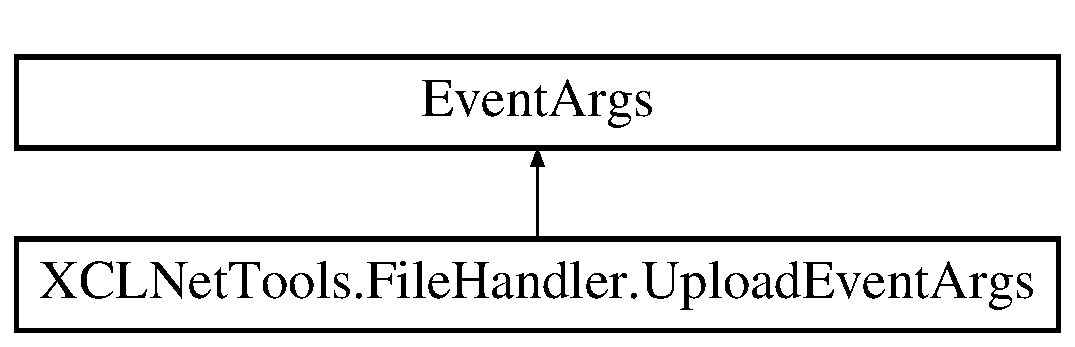
\includegraphics[height=2.000000cm]{class_x_c_l_net_tools_1_1_file_handler_1_1_upload_event_args}
\end{center}
\end{figure}
\subsection*{属性}
\begin{DoxyCompactItemize}
\item 
int \hyperlink{class_x_c_l_net_tools_1_1_file_handler_1_1_upload_event_args_aeb753c87413d86d610121060635794e1}{Bytes\+Sent}\hspace{0.3cm}{\ttfamily  \mbox{[}get, set\mbox{]}}
\begin{DoxyCompactList}\small\item\em 已发送的字节数 \end{DoxyCompactList}\item 
int \hyperlink{class_x_c_l_net_tools_1_1_file_handler_1_1_upload_event_args_a874a8bc16016a3d11eb9aa52f9670eb4}{Total\+Bytes}\hspace{0.3cm}{\ttfamily  \mbox{[}get, set\mbox{]}}
\begin{DoxyCompactList}\small\item\em 总字节数 \end{DoxyCompactList}\end{DoxyCompactItemize}


\subsection{详细描述}
上传数据参数 



在文件 Http\+Proc.\+cs 第 23 行定义.



\subsection{属性说明}
\index{X\+C\+L\+Net\+Tools\+::\+File\+Handler\+::\+Upload\+Event\+Args@{X\+C\+L\+Net\+Tools\+::\+File\+Handler\+::\+Upload\+Event\+Args}!Bytes\+Sent@{Bytes\+Sent}}
\index{Bytes\+Sent@{Bytes\+Sent}!X\+C\+L\+Net\+Tools\+::\+File\+Handler\+::\+Upload\+Event\+Args@{X\+C\+L\+Net\+Tools\+::\+File\+Handler\+::\+Upload\+Event\+Args}}
\subsubsection[{\texorpdfstring{Bytes\+Sent}{BytesSent}}]{\setlength{\rightskip}{0pt plus 5cm}int X\+C\+L\+Net\+Tools.\+File\+Handler.\+Upload\+Event\+Args.\+Bytes\+Sent\hspace{0.3cm}{\ttfamily [get]}, {\ttfamily [set]}}\hypertarget{class_x_c_l_net_tools_1_1_file_handler_1_1_upload_event_args_aeb753c87413d86d610121060635794e1}{}\label{class_x_c_l_net_tools_1_1_file_handler_1_1_upload_event_args_aeb753c87413d86d610121060635794e1}


已发送的字节数 



在文件 Http\+Proc.\+cs 第 32 行定义.

\index{X\+C\+L\+Net\+Tools\+::\+File\+Handler\+::\+Upload\+Event\+Args@{X\+C\+L\+Net\+Tools\+::\+File\+Handler\+::\+Upload\+Event\+Args}!Total\+Bytes@{Total\+Bytes}}
\index{Total\+Bytes@{Total\+Bytes}!X\+C\+L\+Net\+Tools\+::\+File\+Handler\+::\+Upload\+Event\+Args@{X\+C\+L\+Net\+Tools\+::\+File\+Handler\+::\+Upload\+Event\+Args}}
\subsubsection[{\texorpdfstring{Total\+Bytes}{TotalBytes}}]{\setlength{\rightskip}{0pt plus 5cm}int X\+C\+L\+Net\+Tools.\+File\+Handler.\+Upload\+Event\+Args.\+Total\+Bytes\hspace{0.3cm}{\ttfamily [get]}, {\ttfamily [set]}}\hypertarget{class_x_c_l_net_tools_1_1_file_handler_1_1_upload_event_args_a874a8bc16016a3d11eb9aa52f9670eb4}{}\label{class_x_c_l_net_tools_1_1_file_handler_1_1_upload_event_args_a874a8bc16016a3d11eb9aa52f9670eb4}


总字节数 



在文件 Http\+Proc.\+cs 第 41 行定义.



该类的文档由以下文件生成\+:\begin{DoxyCompactItemize}
\item 
E\+:/\+Git\+Hub/\+X\+C\+L\+Net\+Tools/\+X\+C\+L\+Net\+Tools/\+File\+Handler/\hyperlink{_http_proc_8cs}{Http\+Proc.\+cs}\end{DoxyCompactItemize}

\hypertarget{class_x_c_l_net_tools_1_1_string_hander_1_1_url_oper}{\section{X\-C\-L\-Net\-Tools.\-String\-Hander.\-Url\-Oper类 参考}
\label{class_x_c_l_net_tools_1_1_string_hander_1_1_url_oper}\index{X\-C\-L\-Net\-Tools.\-String\-Hander.\-Url\-Oper@{X\-C\-L\-Net\-Tools.\-String\-Hander.\-Url\-Oper}}
}


U\-R\-L的操作类  


\subsection*{静态 Public 成员函数}
\begin{DoxyCompactItemize}
\item 
static string \hyperlink{class_x_c_l_net_tools_1_1_string_hander_1_1_url_oper_a63e4554d226a4e22cdf68614d6fdd1c1}{Add\-Param} (string url, string name, string value)
\begin{DoxyCompactList}\small\item\em 添加\-U\-R\-L参数 \end{DoxyCompactList}\item 
static string \hyperlink{class_x_c_l_net_tools_1_1_string_hander_1_1_url_oper_ae4e0043d5ebfc5401f90242992071fdc}{Add\-Param} (string url, Name\-Value\-Collection param)
\begin{DoxyCompactList}\small\item\em 添加\-U\-R\-L参数 \end{DoxyCompactList}\item 
static string \hyperlink{class_x_c_l_net_tools_1_1_string_hander_1_1_url_oper_adda296014d4edff564f69975de4d3171}{Update\-Param} (string url, string param\-Name, string value)
\begin{DoxyCompactList}\small\item\em 更新\-U\-R\-L参数 \end{DoxyCompactList}\item 
static string \hyperlink{class_x_c_l_net_tools_1_1_string_hander_1_1_url_oper_aee0fcf87276a12d12e71d2d905e286e0}{Remove\-Param} (string url, string param\-Name)
\begin{DoxyCompactList}\small\item\em 删除url参数 \end{DoxyCompactList}\item 
static void \hyperlink{class_x_c_l_net_tools_1_1_string_hander_1_1_url_oper_a8786e6cf26b3496627bbcc037ca72ca7}{Parse\-Url} (string url, out string base\-Url, out Name\-Value\-Collection nvc)
\begin{DoxyCompactList}\small\item\em 分析 url 字符串中的参数信息 \end{DoxyCompactList}\item 
static int \hyperlink{class_x_c_l_net_tools_1_1_string_hander_1_1_url_oper_ac5c640bfc662741345164efa1efbc525}{Get\-Url\-Error} (string curl)
\begin{DoxyCompactList}\small\item\em 获取指定\-U\-R\-L的请求状态: 200 -\/ 确定。客户端请求已成功。 201 -\/ 已创建。 202 -\/ 已接受。 400 -\/ 错误的请求 401 -\/ 访问被拒绝 403 -\/ 禁止访问 404 -\/ 未找到 405 -\/ 用来访问本页面的 H\-T\-T\-P 谓词不被允许(方法不被允许) 406 -\/ 客户端浏览器不接受所请求页面的 M\-I\-M\-E 类型。 407 -\/ 要求进行代理身份验证。 412 -\/ 前提条件失败。 413 – 请求实体太大。 414 -\/ 请求 U\-R\-I 太长。 415 – 不支持的媒体类型。 416 – 所请求的范围无法满足。 417 – 执行失败。 423 – 锁定的错误 500 -\/ 内部服务器错误。 501 -\/ 页眉值指定了未实现的配置。 502 -\/ Web 服务器用作网关或代理服务器时收到了无效响应。 503 -\/ 服务不可用。这个错误代码为 I\-I\-S 6.\-0 所专用。 504 -\/ 网关超时。 505 -\/ H\-T\-T\-P 版本不受支持。 /summary$>$ param name=\char`\"{}curl\char`\"{}$>$要请求的\-U\-R\-L

returns$>$状态码\end{DoxyCompactList}\end{DoxyCompactItemize}


\subsection{详细描述}
U\-R\-L的操作类 



在文件 Url\-Oper.\-cs 第 37 行定义.



\subsection{成员函数说明}
\hypertarget{class_x_c_l_net_tools_1_1_string_hander_1_1_url_oper_a63e4554d226a4e22cdf68614d6fdd1c1}{\index{X\-C\-L\-Net\-Tools\-::\-String\-Hander\-::\-Url\-Oper@{X\-C\-L\-Net\-Tools\-::\-String\-Hander\-::\-Url\-Oper}!Add\-Param@{Add\-Param}}
\index{Add\-Param@{Add\-Param}!XCLNetTools::StringHander::UrlOper@{X\-C\-L\-Net\-Tools\-::\-String\-Hander\-::\-Url\-Oper}}
\subsubsection[{Add\-Param}]{\setlength{\rightskip}{0pt plus 5cm}static string X\-C\-L\-Net\-Tools.\-String\-Hander.\-Url\-Oper.\-Add\-Param (
\begin{DoxyParamCaption}
\item[{string}]{url, }
\item[{string}]{name, }
\item[{string}]{value}
\end{DoxyParamCaption}
)\hspace{0.3cm}{\ttfamily [static]}}}\label{class_x_c_l_net_tools_1_1_string_hander_1_1_url_oper_a63e4554d226a4e22cdf68614d6fdd1c1}


添加\-U\-R\-L参数 


\begin{DoxyParams}{参数}
{\em url} & url\\
\hline
{\em name} & 参数名\\
\hline
{\em value} & 参数值\\
\hline
\end{DoxyParams}
\begin{DoxyReturn}{返回}
新的url
\end{DoxyReturn}


在文件 Url\-Oper.\-cs 第 48 行定义.

\hypertarget{class_x_c_l_net_tools_1_1_string_hander_1_1_url_oper_ae4e0043d5ebfc5401f90242992071fdc}{\index{X\-C\-L\-Net\-Tools\-::\-String\-Hander\-::\-Url\-Oper@{X\-C\-L\-Net\-Tools\-::\-String\-Hander\-::\-Url\-Oper}!Add\-Param@{Add\-Param}}
\index{Add\-Param@{Add\-Param}!XCLNetTools::StringHander::UrlOper@{X\-C\-L\-Net\-Tools\-::\-String\-Hander\-::\-Url\-Oper}}
\subsubsection[{Add\-Param}]{\setlength{\rightskip}{0pt plus 5cm}static string X\-C\-L\-Net\-Tools.\-String\-Hander.\-Url\-Oper.\-Add\-Param (
\begin{DoxyParamCaption}
\item[{string}]{url, }
\item[{Name\-Value\-Collection}]{param}
\end{DoxyParamCaption}
)\hspace{0.3cm}{\ttfamily [static]}}}\label{class_x_c_l_net_tools_1_1_string_hander_1_1_url_oper_ae4e0043d5ebfc5401f90242992071fdc}


添加\-U\-R\-L参数 


\begin{DoxyParams}{参数}
{\em url} & url\\
\hline
{\em param} & 参数集合\\
\hline
\end{DoxyParams}
\begin{DoxyReturn}{返回}
新的url
\end{DoxyReturn}


在文件 Url\-Oper.\-cs 第 61 行定义.

\hypertarget{class_x_c_l_net_tools_1_1_string_hander_1_1_url_oper_ac5c640bfc662741345164efa1efbc525}{\index{X\-C\-L\-Net\-Tools\-::\-String\-Hander\-::\-Url\-Oper@{X\-C\-L\-Net\-Tools\-::\-String\-Hander\-::\-Url\-Oper}!Get\-Url\-Error@{Get\-Url\-Error}}
\index{Get\-Url\-Error@{Get\-Url\-Error}!XCLNetTools::StringHander::UrlOper@{X\-C\-L\-Net\-Tools\-::\-String\-Hander\-::\-Url\-Oper}}
\subsubsection[{Get\-Url\-Error}]{\setlength{\rightskip}{0pt plus 5cm}static int X\-C\-L\-Net\-Tools.\-String\-Hander.\-Url\-Oper.\-Get\-Url\-Error (
\begin{DoxyParamCaption}
\item[{string}]{curl}
\end{DoxyParamCaption}
)\hspace{0.3cm}{\ttfamily [static]}}}\label{class_x_c_l_net_tools_1_1_string_hander_1_1_url_oper_ac5c640bfc662741345164efa1efbc525}


获取指定\-U\-R\-L的请求状态: 200 -\/ 确定。客户端请求已成功。 201 -\/ 已创建。 202 -\/ 已接受。 400 -\/ 错误的请求 401 -\/ 访问被拒绝 403 -\/ 禁止访问 404 -\/ 未找到 405 -\/ 用来访问本页面的 H\-T\-T\-P 谓词不被允许(方法不被允许) 406 -\/ 客户端浏览器不接受所请求页面的 M\-I\-M\-E 类型。 407 -\/ 要求进行代理身份验证。 412 -\/ 前提条件失败。 413 – 请求实体太大。 414 -\/ 请求 U\-R\-I 太长。 415 – 不支持的媒体类型。 416 – 所请求的范围无法满足。 417 – 执行失败。 423 – 锁定的错误 500 -\/ 内部服务器错误。 501 -\/ 页眉值指定了未实现的配置。 502 -\/ Web 服务器用作网关或代理服务器时收到了无效响应。 503 -\/ 服务不可用。这个错误代码为 I\-I\-S 6.\-0 所专用。 504 -\/ 网关超时。 505 -\/ H\-T\-T\-P 版本不受支持。 /summary$>$ param name=\char`\"{}curl\char`\"{}$>$要请求的\-U\-R\-L

returns$>$状态码



在文件 Url\-Oper.\-cs 第 238 行定义.

\hypertarget{class_x_c_l_net_tools_1_1_string_hander_1_1_url_oper_a8786e6cf26b3496627bbcc037ca72ca7}{\index{X\-C\-L\-Net\-Tools\-::\-String\-Hander\-::\-Url\-Oper@{X\-C\-L\-Net\-Tools\-::\-String\-Hander\-::\-Url\-Oper}!Parse\-Url@{Parse\-Url}}
\index{Parse\-Url@{Parse\-Url}!XCLNetTools::StringHander::UrlOper@{X\-C\-L\-Net\-Tools\-::\-String\-Hander\-::\-Url\-Oper}}
\subsubsection[{Parse\-Url}]{\setlength{\rightskip}{0pt plus 5cm}static void X\-C\-L\-Net\-Tools.\-String\-Hander.\-Url\-Oper.\-Parse\-Url (
\begin{DoxyParamCaption}
\item[{string}]{url, }
\item[{out string}]{base\-Url, }
\item[{out Name\-Value\-Collection}]{nvc}
\end{DoxyParamCaption}
)\hspace{0.3cm}{\ttfamily [static]}}}\label{class_x_c_l_net_tools_1_1_string_hander_1_1_url_oper_a8786e6cf26b3496627bbcc037ca72ca7}


分析 url 字符串中的参数信息 


\begin{DoxyParams}{参数}
{\em url} & 输入的 U\-R\-L\\
\hline
{\em base\-Url} & 输出 U\-R\-L 的基础部分\\
\hline
{\em nvc} & 输出分析后得到的 (参数名,参数值) 的集合\\
\hline
\end{DoxyParams}


在文件 Url\-Oper.\-cs 第 175 行定义.

\hypertarget{class_x_c_l_net_tools_1_1_string_hander_1_1_url_oper_aee0fcf87276a12d12e71d2d905e286e0}{\index{X\-C\-L\-Net\-Tools\-::\-String\-Hander\-::\-Url\-Oper@{X\-C\-L\-Net\-Tools\-::\-String\-Hander\-::\-Url\-Oper}!Remove\-Param@{Remove\-Param}}
\index{Remove\-Param@{Remove\-Param}!XCLNetTools::StringHander::UrlOper@{X\-C\-L\-Net\-Tools\-::\-String\-Hander\-::\-Url\-Oper}}
\subsubsection[{Remove\-Param}]{\setlength{\rightskip}{0pt plus 5cm}static string X\-C\-L\-Net\-Tools.\-String\-Hander.\-Url\-Oper.\-Remove\-Param (
\begin{DoxyParamCaption}
\item[{string}]{url, }
\item[{string}]{param\-Name}
\end{DoxyParamCaption}
)\hspace{0.3cm}{\ttfamily [static]}}}\label{class_x_c_l_net_tools_1_1_string_hander_1_1_url_oper_aee0fcf87276a12d12e71d2d905e286e0}


删除url参数 


\begin{DoxyParams}{参数}
{\em url} & url\\
\hline
{\em param\-Name} & 参数名\\
\hline
\end{DoxyParams}
\begin{DoxyReturn}{返回}
新的url
\end{DoxyReturn}


在文件 Url\-Oper.\-cs 第 126 行定义.

\hypertarget{class_x_c_l_net_tools_1_1_string_hander_1_1_url_oper_adda296014d4edff564f69975de4d3171}{\index{X\-C\-L\-Net\-Tools\-::\-String\-Hander\-::\-Url\-Oper@{X\-C\-L\-Net\-Tools\-::\-String\-Hander\-::\-Url\-Oper}!Update\-Param@{Update\-Param}}
\index{Update\-Param@{Update\-Param}!XCLNetTools::StringHander::UrlOper@{X\-C\-L\-Net\-Tools\-::\-String\-Hander\-::\-Url\-Oper}}
\subsubsection[{Update\-Param}]{\setlength{\rightskip}{0pt plus 5cm}static string X\-C\-L\-Net\-Tools.\-String\-Hander.\-Url\-Oper.\-Update\-Param (
\begin{DoxyParamCaption}
\item[{string}]{url, }
\item[{string}]{param\-Name, }
\item[{string}]{value}
\end{DoxyParamCaption}
)\hspace{0.3cm}{\ttfamily [static]}}}\label{class_x_c_l_net_tools_1_1_string_hander_1_1_url_oper_adda296014d4edff564f69975de4d3171}


更新\-U\-R\-L参数 


\begin{DoxyParams}{参数}
{\em url} & url\\
\hline
{\em param\-Name} & 参数名\\
\hline
{\em value} & 参数值\\
\hline
\end{DoxyParams}
\begin{DoxyReturn}{返回}
新的url
\end{DoxyReturn}


在文件 Url\-Oper.\-cs 第 104 行定义.



该类的文档由以下文件生成\-:\begin{DoxyCompactItemize}
\item 
D\-:/\-My\-Data/\-My\-Git/\-Git\-Hub/\-X\-C\-L\-Net\-Tools/\-X\-C\-L\-Net\-Tools/\-String\-Hander/\hyperlink{_url_oper_8cs}{Url\-Oper.\-cs}\end{DoxyCompactItemize}

\hypertarget{class_x_c_l_net_tools_1_1_file_handler_1_1_verification_code}{\section{X\-C\-L\-Net\-Tools.\-File\-Handler.\-Verification\-Code类 参考}
\label{class_x_c_l_net_tools_1_1_file_handler_1_1_verification_code}\index{X\-C\-L\-Net\-Tools.\-File\-Handler.\-Verification\-Code@{X\-C\-L\-Net\-Tools.\-File\-Handler.\-Verification\-Code}}
}


验证码相关  


\subsection*{静态 Public 成员函数}
\begin{DoxyCompactItemize}
\item 
static string \hyperlink{class_x_c_l_net_tools_1_1_file_handler_1_1_verification_code_af4beced22b07b395e6ae37452a895f32}{Generate\-Check\-Code} ()
\begin{DoxyCompactList}\small\item\em 生成验证码的随机数 \end{DoxyCompactList}\item 
static void \hyperlink{class_x_c_l_net_tools_1_1_file_handler_1_1_verification_code_acde0d83935e0d55da7a29725026a72e9}{Create\-Check\-Code\-Image} (string check\-Code)
\begin{DoxyCompactList}\small\item\em 生成验证码图片 \end{DoxyCompactList}\end{DoxyCompactItemize}


\subsection{详细描述}
验证码相关 



在文件 Verification\-Code.\-cs 第 18 行定义.



\subsection{成员函数说明}
\hypertarget{class_x_c_l_net_tools_1_1_file_handler_1_1_verification_code_acde0d83935e0d55da7a29725026a72e9}{\index{X\-C\-L\-Net\-Tools\-::\-File\-Handler\-::\-Verification\-Code@{X\-C\-L\-Net\-Tools\-::\-File\-Handler\-::\-Verification\-Code}!Create\-Check\-Code\-Image@{Create\-Check\-Code\-Image}}
\index{Create\-Check\-Code\-Image@{Create\-Check\-Code\-Image}!XCLNetTools::FileHandler::VerificationCode@{X\-C\-L\-Net\-Tools\-::\-File\-Handler\-::\-Verification\-Code}}
\subsubsection[{Create\-Check\-Code\-Image}]{\setlength{\rightskip}{0pt plus 5cm}static void X\-C\-L\-Net\-Tools.\-File\-Handler.\-Verification\-Code.\-Create\-Check\-Code\-Image (
\begin{DoxyParamCaption}
\item[{string}]{check\-Code}
\end{DoxyParamCaption}
)\hspace{0.3cm}{\ttfamily [static]}}}\label{class_x_c_l_net_tools_1_1_file_handler_1_1_verification_code_acde0d83935e0d55da7a29725026a72e9}


生成验证码图片 


\begin{DoxyParams}{参数}
{\em check\-Code} & 字符代码\\
\hline
\end{DoxyParams}


在文件 Verification\-Code.\-cs 第 46 行定义.

\hypertarget{class_x_c_l_net_tools_1_1_file_handler_1_1_verification_code_af4beced22b07b395e6ae37452a895f32}{\index{X\-C\-L\-Net\-Tools\-::\-File\-Handler\-::\-Verification\-Code@{X\-C\-L\-Net\-Tools\-::\-File\-Handler\-::\-Verification\-Code}!Generate\-Check\-Code@{Generate\-Check\-Code}}
\index{Generate\-Check\-Code@{Generate\-Check\-Code}!XCLNetTools::FileHandler::VerificationCode@{X\-C\-L\-Net\-Tools\-::\-File\-Handler\-::\-Verification\-Code}}
\subsubsection[{Generate\-Check\-Code}]{\setlength{\rightskip}{0pt plus 5cm}static string X\-C\-L\-Net\-Tools.\-File\-Handler.\-Verification\-Code.\-Generate\-Check\-Code (
\begin{DoxyParamCaption}
{}
\end{DoxyParamCaption}
)\hspace{0.3cm}{\ttfamily [static]}}}\label{class_x_c_l_net_tools_1_1_file_handler_1_1_verification_code_af4beced22b07b395e6ae37452a895f32}


生成验证码的随机数 

\begin{DoxyReturn}{返回}
随机数
\end{DoxyReturn}


在文件 Verification\-Code.\-cs 第 24 行定义.



该类的文档由以下文件生成\-:\begin{DoxyCompactItemize}
\item 
D\-:/\-My\-Data/\-My\-Git/\-Git\-Hub/\-X\-C\-L\-Net\-Tools/\-X\-C\-L\-Net\-Tools/\-File\-Handler/\hyperlink{_verification_code_8cs}{Verification\-Code.\-cs}\end{DoxyCompactItemize}

\hypertarget{class_x_c_l_net_tools_1_1_file_handler_1_1_web_client}{}\section{X\+C\+L\+Net\+Tools.\+File\+Handler.\+Web\+Client类 参考}
\label{class_x_c_l_net_tools_1_1_file_handler_1_1_web_client}\index{X\+C\+L\+Net\+Tools.\+File\+Handler.\+Web\+Client@{X\+C\+L\+Net\+Tools.\+File\+Handler.\+Web\+Client}}


\hyperlink{class_x_c_l_net_tools_1_1_file_handler_1_1_web_client}{Web\+Client}  


\subsection*{Public 成员函数}
\begin{DoxyCompactItemize}
\item 
\hyperlink{class_x_c_l_net_tools_1_1_file_handler_1_1_web_client_a8f3cbaf1baf5d142caab2f6c9cc04a7f}{Web\+Client} ()
\begin{DoxyCompactList}\small\item\em 创建\+Web\+Client的实例 \end{DoxyCompactList}\item 
string \hyperlink{class_x_c_l_net_tools_1_1_file_handler_1_1_web_client_a504910f5e28a6fa620853f069d3c756b}{Get\+Html} (string url)
\begin{DoxyCompactList}\small\item\em 获取网页源代码 \end{DoxyCompactList}\item 
void \hyperlink{class_x_c_l_net_tools_1_1_file_handler_1_1_web_client_ace80aaf94d3e0c6eceb3ad182b8de947}{Download\+File} (string url, string filename)
\begin{DoxyCompactList}\small\item\em 下载文件 \end{DoxyCompactList}\item 
byte \mbox{[}$\,$\mbox{]} \hyperlink{class_x_c_l_net_tools_1_1_file_handler_1_1_web_client_a7208770077f210c3dd7bee2b34f0a4eb}{Get\+Data} (string url)
\begin{DoxyCompactList}\small\item\em 从指定\+U\+R\+L下载数据 \end{DoxyCompactList}\item 
string \hyperlink{class_x_c_l_net_tools_1_1_file_handler_1_1_web_client_ab2497ff9ed5a5b867362b7bc0b38edb1}{Post} (string url, string post\+Data)
\begin{DoxyCompactList}\small\item\em 向指定\+U\+R\+L发送文本数据 \end{DoxyCompactList}\item 
string \hyperlink{class_x_c_l_net_tools_1_1_file_handler_1_1_web_client_ad799cba2f787fba4c0ca4fc6e86ee831}{Post} (string url, byte\mbox{[}$\,$\mbox{]} post\+Data)
\begin{DoxyCompactList}\small\item\em 向指定\+U\+R\+L发送字节数据 \end{DoxyCompactList}\item 
string \hyperlink{class_x_c_l_net_tools_1_1_file_handler_1_1_web_client_ab1556a7a601a8425c7d6bcecb09d6cf2}{Post} (string url, \hyperlink{class_x_c_l_net_tools_1_1_file_handler_1_1_multipart_form}{Multipart\+Form} mulitpart\+Form)
\begin{DoxyCompactList}\small\item\em 向指定网址发送mulitpart编码的数据 \end{DoxyCompactList}\end{DoxyCompactItemize}
\subsection*{属性}
\begin{DoxyCompactItemize}
\item 
int \hyperlink{class_x_c_l_net_tools_1_1_file_handler_1_1_web_client_a192f27c95b8274758ca9d68c620de7c3}{Buffer\+Size}\hspace{0.3cm}{\ttfamily  \mbox{[}get, set\mbox{]}}
\begin{DoxyCompactList}\small\item\em 设置发送和接收的数据缓冲大小 \end{DoxyCompactList}\item 
Web\+Header\+Collection \hyperlink{class_x_c_l_net_tools_1_1_file_handler_1_1_web_client_a3d00d3457c23ce30274af963f4cab6bb}{Response\+Headers}\hspace{0.3cm}{\ttfamily  \mbox{[}get\mbox{]}}
\begin{DoxyCompactList}\small\item\em 获取响应头集合 \end{DoxyCompactList}\item 
Web\+Header\+Collection \hyperlink{class_x_c_l_net_tools_1_1_file_handler_1_1_web_client_a89d4bf2af70a2a0991904b1b61c8dd1d}{Request\+Headers}\hspace{0.3cm}{\ttfamily  \mbox{[}get\mbox{]}}
\begin{DoxyCompactList}\small\item\em 获取请求头集合 \end{DoxyCompactList}\item 
Web\+Proxy \hyperlink{class_x_c_l_net_tools_1_1_file_handler_1_1_web_client_ac2f17eefdc2372eb01a6be915d19c0ba}{Proxy}\hspace{0.3cm}{\ttfamily  \mbox{[}get, set\mbox{]}}
\begin{DoxyCompactList}\small\item\em 获取或设置代理 \end{DoxyCompactList}\item 
Encoding \hyperlink{class_x_c_l_net_tools_1_1_file_handler_1_1_web_client_a9bd02ab7f0198d34a44487c5d8c02f19}{Encoding}\hspace{0.3cm}{\ttfamily  \mbox{[}get, set\mbox{]}}
\begin{DoxyCompactList}\small\item\em 获取或设置请求与响应的文本编码方式 \end{DoxyCompactList}\item 
string \hyperlink{class_x_c_l_net_tools_1_1_file_handler_1_1_web_client_a67e90e96bd067171c16cb84d75f66c3a}{Resp\+Html}\hspace{0.3cm}{\ttfamily  \mbox{[}get, set\mbox{]}}
\begin{DoxyCompactList}\small\item\em 获取或设置响应的html代码 \end{DoxyCompactList}\item 
Cookie\+Container \hyperlink{class_x_c_l_net_tools_1_1_file_handler_1_1_web_client_adeaa1201074e43df3743d76ea77cf06e}{Cookie\+Container}\hspace{0.3cm}{\ttfamily  \mbox{[}get, set\mbox{]}}
\begin{DoxyCompactList}\small\item\em 获取或设置与请求关联的\+Cookie容器 \end{DoxyCompactList}\end{DoxyCompactItemize}
\subsection*{事件}
\begin{DoxyCompactItemize}
\item 
Event\+Handler$<$ \hyperlink{class_x_c_l_net_tools_1_1_file_handler_1_1_upload_event_args}{Upload\+Event\+Args} $>$ \hyperlink{class_x_c_l_net_tools_1_1_file_handler_1_1_web_client_abe950fa329508b4c52e3181aeb97585f}{Upload\+Progress\+Changed}
\begin{DoxyCompactList}\small\item\em 上传事件 \end{DoxyCompactList}\item 
Event\+Handler$<$ \hyperlink{class_x_c_l_net_tools_1_1_file_handler_1_1_download_event_args}{Download\+Event\+Args} $>$ \hyperlink{class_x_c_l_net_tools_1_1_file_handler_1_1_web_client_aa1e50d608381b728356547eff9f80213}{Download\+Progress\+Changed}
\begin{DoxyCompactList}\small\item\em 下载事件 \end{DoxyCompactList}\end{DoxyCompactItemize}


\subsection{详细描述}
\hyperlink{class_x_c_l_net_tools_1_1_file_handler_1_1_web_client}{Web\+Client} 



在文件 Http\+Proc.\+cs 第 87 行定义.



\subsection{构造及析构函数说明}
\mbox{\Hypertarget{class_x_c_l_net_tools_1_1_file_handler_1_1_web_client_a8f3cbaf1baf5d142caab2f6c9cc04a7f}\label{class_x_c_l_net_tools_1_1_file_handler_1_1_web_client_a8f3cbaf1baf5d142caab2f6c9cc04a7f}} 
\index{X\+C\+L\+Net\+Tools\+::\+File\+Handler\+::\+Web\+Client@{X\+C\+L\+Net\+Tools\+::\+File\+Handler\+::\+Web\+Client}!Web\+Client@{Web\+Client}}
\index{Web\+Client@{Web\+Client}!X\+C\+L\+Net\+Tools\+::\+File\+Handler\+::\+Web\+Client@{X\+C\+L\+Net\+Tools\+::\+File\+Handler\+::\+Web\+Client}}
\subsubsection{\texorpdfstring{Web\+Client()}{WebClient()}}
{\footnotesize\ttfamily X\+C\+L\+Net\+Tools.\+File\+Handler.\+Web\+Client.\+Web\+Client (\begin{DoxyParamCaption}{ }\end{DoxyParamCaption})}



创建\+Web\+Client的实例 



在文件 Http\+Proc.\+cs 第 115 行定义.



\subsection{成员函数说明}
\mbox{\Hypertarget{class_x_c_l_net_tools_1_1_file_handler_1_1_web_client_ace80aaf94d3e0c6eceb3ad182b8de947}\label{class_x_c_l_net_tools_1_1_file_handler_1_1_web_client_ace80aaf94d3e0c6eceb3ad182b8de947}} 
\index{X\+C\+L\+Net\+Tools\+::\+File\+Handler\+::\+Web\+Client@{X\+C\+L\+Net\+Tools\+::\+File\+Handler\+::\+Web\+Client}!Download\+File@{Download\+File}}
\index{Download\+File@{Download\+File}!X\+C\+L\+Net\+Tools\+::\+File\+Handler\+::\+Web\+Client@{X\+C\+L\+Net\+Tools\+::\+File\+Handler\+::\+Web\+Client}}
\subsubsection{\texorpdfstring{Download\+File()}{DownloadFile()}}
{\footnotesize\ttfamily void X\+C\+L\+Net\+Tools.\+File\+Handler.\+Web\+Client.\+Download\+File (\begin{DoxyParamCaption}\item[{string}]{url,  }\item[{string}]{filename }\end{DoxyParamCaption})}



下载文件 


\begin{DoxyParams}{参数}
{\em url} & 文件\+U\+R\+L地址\\
\hline
{\em filename} & 文件保存完整路径\\
\hline
\end{DoxyParams}


在文件 Http\+Proc.\+cs 第 199 行定义.

\mbox{\Hypertarget{class_x_c_l_net_tools_1_1_file_handler_1_1_web_client_a7208770077f210c3dd7bee2b34f0a4eb}\label{class_x_c_l_net_tools_1_1_file_handler_1_1_web_client_a7208770077f210c3dd7bee2b34f0a4eb}} 
\index{X\+C\+L\+Net\+Tools\+::\+File\+Handler\+::\+Web\+Client@{X\+C\+L\+Net\+Tools\+::\+File\+Handler\+::\+Web\+Client}!Get\+Data@{Get\+Data}}
\index{Get\+Data@{Get\+Data}!X\+C\+L\+Net\+Tools\+::\+File\+Handler\+::\+Web\+Client@{X\+C\+L\+Net\+Tools\+::\+File\+Handler\+::\+Web\+Client}}
\subsubsection{\texorpdfstring{Get\+Data()}{GetData()}}
{\footnotesize\ttfamily byte \mbox{[}$\,$\mbox{]} X\+C\+L\+Net\+Tools.\+File\+Handler.\+Web\+Client.\+Get\+Data (\begin{DoxyParamCaption}\item[{string}]{url }\end{DoxyParamCaption})}



从指定\+U\+R\+L下载数据 


\begin{DoxyParams}{参数}
{\em url} & 网址\\
\hline
\end{DoxyParams}
\begin{DoxyReturn}{返回}

\end{DoxyReturn}


在文件 Http\+Proc.\+cs 第 220 行定义.

\mbox{\Hypertarget{class_x_c_l_net_tools_1_1_file_handler_1_1_web_client_a504910f5e28a6fa620853f069d3c756b}\label{class_x_c_l_net_tools_1_1_file_handler_1_1_web_client_a504910f5e28a6fa620853f069d3c756b}} 
\index{X\+C\+L\+Net\+Tools\+::\+File\+Handler\+::\+Web\+Client@{X\+C\+L\+Net\+Tools\+::\+File\+Handler\+::\+Web\+Client}!Get\+Html@{Get\+Html}}
\index{Get\+Html@{Get\+Html}!X\+C\+L\+Net\+Tools\+::\+File\+Handler\+::\+Web\+Client@{X\+C\+L\+Net\+Tools\+::\+File\+Handler\+::\+Web\+Client}}
\subsubsection{\texorpdfstring{Get\+Html()}{GetHtml()}}
{\footnotesize\ttfamily string X\+C\+L\+Net\+Tools.\+File\+Handler.\+Web\+Client.\+Get\+Html (\begin{DoxyParamCaption}\item[{string}]{url }\end{DoxyParamCaption})}



获取网页源代码 


\begin{DoxyParams}{参数}
{\em url} & 网址\\
\hline
\end{DoxyParams}
\begin{DoxyReturn}{返回}

\end{DoxyReturn}


在文件 Http\+Proc.\+cs 第 187 行定义.

\mbox{\Hypertarget{class_x_c_l_net_tools_1_1_file_handler_1_1_web_client_ab2497ff9ed5a5b867362b7bc0b38edb1}\label{class_x_c_l_net_tools_1_1_file_handler_1_1_web_client_ab2497ff9ed5a5b867362b7bc0b38edb1}} 
\index{X\+C\+L\+Net\+Tools\+::\+File\+Handler\+::\+Web\+Client@{X\+C\+L\+Net\+Tools\+::\+File\+Handler\+::\+Web\+Client}!Post@{Post}}
\index{Post@{Post}!X\+C\+L\+Net\+Tools\+::\+File\+Handler\+::\+Web\+Client@{X\+C\+L\+Net\+Tools\+::\+File\+Handler\+::\+Web\+Client}}
\subsubsection{\texorpdfstring{Post()}{Post()}\hspace{0.1cm}{\footnotesize\ttfamily [1/3]}}
{\footnotesize\ttfamily string X\+C\+L\+Net\+Tools.\+File\+Handler.\+Web\+Client.\+Post (\begin{DoxyParamCaption}\item[{string}]{url,  }\item[{string}]{post\+Data }\end{DoxyParamCaption})}



向指定\+U\+R\+L发送文本数据 


\begin{DoxyParams}{参数}
{\em url} & 网址\\
\hline
{\em post\+Data} & urlencode编码的文本数据\\
\hline
\end{DoxyParams}
\begin{DoxyReturn}{返回}

\end{DoxyReturn}


在文件 Http\+Proc.\+cs 第 232 行定义.

\mbox{\Hypertarget{class_x_c_l_net_tools_1_1_file_handler_1_1_web_client_ad799cba2f787fba4c0ca4fc6e86ee831}\label{class_x_c_l_net_tools_1_1_file_handler_1_1_web_client_ad799cba2f787fba4c0ca4fc6e86ee831}} 
\index{X\+C\+L\+Net\+Tools\+::\+File\+Handler\+::\+Web\+Client@{X\+C\+L\+Net\+Tools\+::\+File\+Handler\+::\+Web\+Client}!Post@{Post}}
\index{Post@{Post}!X\+C\+L\+Net\+Tools\+::\+File\+Handler\+::\+Web\+Client@{X\+C\+L\+Net\+Tools\+::\+File\+Handler\+::\+Web\+Client}}
\subsubsection{\texorpdfstring{Post()}{Post()}\hspace{0.1cm}{\footnotesize\ttfamily [2/3]}}
{\footnotesize\ttfamily string X\+C\+L\+Net\+Tools.\+File\+Handler.\+Web\+Client.\+Post (\begin{DoxyParamCaption}\item[{string}]{url,  }\item[{byte \mbox{[}$\,$\mbox{]}}]{post\+Data }\end{DoxyParamCaption})}



向指定\+U\+R\+L发送字节数据 


\begin{DoxyParams}{参数}
{\em url} & 网址\\
\hline
{\em post\+Data} & 发送的字节数组\\
\hline
\end{DoxyParams}
\begin{DoxyReturn}{返回}

\end{DoxyReturn}


在文件 Http\+Proc.\+cs 第 244 行定义.

\mbox{\Hypertarget{class_x_c_l_net_tools_1_1_file_handler_1_1_web_client_ab1556a7a601a8425c7d6bcecb09d6cf2}\label{class_x_c_l_net_tools_1_1_file_handler_1_1_web_client_ab1556a7a601a8425c7d6bcecb09d6cf2}} 
\index{X\+C\+L\+Net\+Tools\+::\+File\+Handler\+::\+Web\+Client@{X\+C\+L\+Net\+Tools\+::\+File\+Handler\+::\+Web\+Client}!Post@{Post}}
\index{Post@{Post}!X\+C\+L\+Net\+Tools\+::\+File\+Handler\+::\+Web\+Client@{X\+C\+L\+Net\+Tools\+::\+File\+Handler\+::\+Web\+Client}}
\subsubsection{\texorpdfstring{Post()}{Post()}\hspace{0.1cm}{\footnotesize\ttfamily [3/3]}}
{\footnotesize\ttfamily string X\+C\+L\+Net\+Tools.\+File\+Handler.\+Web\+Client.\+Post (\begin{DoxyParamCaption}\item[{string}]{url,  }\item[{\hyperlink{class_x_c_l_net_tools_1_1_file_handler_1_1_multipart_form}{Multipart\+Form}}]{mulitpart\+Form }\end{DoxyParamCaption})}



向指定网址发送mulitpart编码的数据 


\begin{DoxyParams}{参数}
{\em url} & 网址\\
\hline
{\em mulitpart\+Form} & mulitpart form data\\
\hline
\end{DoxyParams}
\begin{DoxyReturn}{返回}

\end{DoxyReturn}


在文件 Http\+Proc.\+cs 第 261 行定义.



\subsection{属性说明}
\mbox{\Hypertarget{class_x_c_l_net_tools_1_1_file_handler_1_1_web_client_a192f27c95b8274758ca9d68c620de7c3}\label{class_x_c_l_net_tools_1_1_file_handler_1_1_web_client_a192f27c95b8274758ca9d68c620de7c3}} 
\index{X\+C\+L\+Net\+Tools\+::\+File\+Handler\+::\+Web\+Client@{X\+C\+L\+Net\+Tools\+::\+File\+Handler\+::\+Web\+Client}!Buffer\+Size@{Buffer\+Size}}
\index{Buffer\+Size@{Buffer\+Size}!X\+C\+L\+Net\+Tools\+::\+File\+Handler\+::\+Web\+Client@{X\+C\+L\+Net\+Tools\+::\+File\+Handler\+::\+Web\+Client}}
\subsubsection{\texorpdfstring{Buffer\+Size}{BufferSize}}
{\footnotesize\ttfamily int X\+C\+L\+Net\+Tools.\+File\+Handler.\+Web\+Client.\+Buffer\+Size\hspace{0.3cm}{\ttfamily [get]}, {\ttfamily [set]}}



设置发送和接收的数据缓冲大小 



在文件 Http\+Proc.\+cs 第 125 行定义.

\mbox{\Hypertarget{class_x_c_l_net_tools_1_1_file_handler_1_1_web_client_adeaa1201074e43df3743d76ea77cf06e}\label{class_x_c_l_net_tools_1_1_file_handler_1_1_web_client_adeaa1201074e43df3743d76ea77cf06e}} 
\index{X\+C\+L\+Net\+Tools\+::\+File\+Handler\+::\+Web\+Client@{X\+C\+L\+Net\+Tools\+::\+File\+Handler\+::\+Web\+Client}!Cookie\+Container@{Cookie\+Container}}
\index{Cookie\+Container@{Cookie\+Container}!X\+C\+L\+Net\+Tools\+::\+File\+Handler\+::\+Web\+Client@{X\+C\+L\+Net\+Tools\+::\+File\+Handler\+::\+Web\+Client}}
\subsubsection{\texorpdfstring{Cookie\+Container}{CookieContainer}}
{\footnotesize\ttfamily Cookie\+Container X\+C\+L\+Net\+Tools.\+File\+Handler.\+Web\+Client.\+Cookie\+Container\hspace{0.3cm}{\ttfamily [get]}, {\ttfamily [set]}}



获取或设置与请求关联的\+Cookie容器 



在文件 Http\+Proc.\+cs 第 177 行定义.

\mbox{\Hypertarget{class_x_c_l_net_tools_1_1_file_handler_1_1_web_client_a9bd02ab7f0198d34a44487c5d8c02f19}\label{class_x_c_l_net_tools_1_1_file_handler_1_1_web_client_a9bd02ab7f0198d34a44487c5d8c02f19}} 
\index{X\+C\+L\+Net\+Tools\+::\+File\+Handler\+::\+Web\+Client@{X\+C\+L\+Net\+Tools\+::\+File\+Handler\+::\+Web\+Client}!Encoding@{Encoding}}
\index{Encoding@{Encoding}!X\+C\+L\+Net\+Tools\+::\+File\+Handler\+::\+Web\+Client@{X\+C\+L\+Net\+Tools\+::\+File\+Handler\+::\+Web\+Client}}
\subsubsection{\texorpdfstring{Encoding}{Encoding}}
{\footnotesize\ttfamily Encoding X\+C\+L\+Net\+Tools.\+File\+Handler.\+Web\+Client.\+Encoding\hspace{0.3cm}{\ttfamily [get]}, {\ttfamily [set]}}



获取或设置请求与响应的文本编码方式 



在文件 Http\+Proc.\+cs 第 159 行定义.

\mbox{\Hypertarget{class_x_c_l_net_tools_1_1_file_handler_1_1_web_client_ac2f17eefdc2372eb01a6be915d19c0ba}\label{class_x_c_l_net_tools_1_1_file_handler_1_1_web_client_ac2f17eefdc2372eb01a6be915d19c0ba}} 
\index{X\+C\+L\+Net\+Tools\+::\+File\+Handler\+::\+Web\+Client@{X\+C\+L\+Net\+Tools\+::\+File\+Handler\+::\+Web\+Client}!Proxy@{Proxy}}
\index{Proxy@{Proxy}!X\+C\+L\+Net\+Tools\+::\+File\+Handler\+::\+Web\+Client@{X\+C\+L\+Net\+Tools\+::\+File\+Handler\+::\+Web\+Client}}
\subsubsection{\texorpdfstring{Proxy}{Proxy}}
{\footnotesize\ttfamily Web\+Proxy X\+C\+L\+Net\+Tools.\+File\+Handler.\+Web\+Client.\+Proxy\hspace{0.3cm}{\ttfamily [get]}, {\ttfamily [set]}}



获取或设置代理 



在文件 Http\+Proc.\+cs 第 150 行定义.

\mbox{\Hypertarget{class_x_c_l_net_tools_1_1_file_handler_1_1_web_client_a89d4bf2af70a2a0991904b1b61c8dd1d}\label{class_x_c_l_net_tools_1_1_file_handler_1_1_web_client_a89d4bf2af70a2a0991904b1b61c8dd1d}} 
\index{X\+C\+L\+Net\+Tools\+::\+File\+Handler\+::\+Web\+Client@{X\+C\+L\+Net\+Tools\+::\+File\+Handler\+::\+Web\+Client}!Request\+Headers@{Request\+Headers}}
\index{Request\+Headers@{Request\+Headers}!X\+C\+L\+Net\+Tools\+::\+File\+Handler\+::\+Web\+Client@{X\+C\+L\+Net\+Tools\+::\+File\+Handler\+::\+Web\+Client}}
\subsubsection{\texorpdfstring{Request\+Headers}{RequestHeaders}}
{\footnotesize\ttfamily Web\+Header\+Collection X\+C\+L\+Net\+Tools.\+File\+Handler.\+Web\+Client.\+Request\+Headers\hspace{0.3cm}{\ttfamily [get]}}



获取请求头集合 



在文件 Http\+Proc.\+cs 第 142 行定义.

\mbox{\Hypertarget{class_x_c_l_net_tools_1_1_file_handler_1_1_web_client_a67e90e96bd067171c16cb84d75f66c3a}\label{class_x_c_l_net_tools_1_1_file_handler_1_1_web_client_a67e90e96bd067171c16cb84d75f66c3a}} 
\index{X\+C\+L\+Net\+Tools\+::\+File\+Handler\+::\+Web\+Client@{X\+C\+L\+Net\+Tools\+::\+File\+Handler\+::\+Web\+Client}!Resp\+Html@{Resp\+Html}}
\index{Resp\+Html@{Resp\+Html}!X\+C\+L\+Net\+Tools\+::\+File\+Handler\+::\+Web\+Client@{X\+C\+L\+Net\+Tools\+::\+File\+Handler\+::\+Web\+Client}}
\subsubsection{\texorpdfstring{Resp\+Html}{RespHtml}}
{\footnotesize\ttfamily string X\+C\+L\+Net\+Tools.\+File\+Handler.\+Web\+Client.\+Resp\+Html\hspace{0.3cm}{\ttfamily [get]}, {\ttfamily [set]}}



获取或设置响应的html代码 



在文件 Http\+Proc.\+cs 第 168 行定义.

\mbox{\Hypertarget{class_x_c_l_net_tools_1_1_file_handler_1_1_web_client_a3d00d3457c23ce30274af963f4cab6bb}\label{class_x_c_l_net_tools_1_1_file_handler_1_1_web_client_a3d00d3457c23ce30274af963f4cab6bb}} 
\index{X\+C\+L\+Net\+Tools\+::\+File\+Handler\+::\+Web\+Client@{X\+C\+L\+Net\+Tools\+::\+File\+Handler\+::\+Web\+Client}!Response\+Headers@{Response\+Headers}}
\index{Response\+Headers@{Response\+Headers}!X\+C\+L\+Net\+Tools\+::\+File\+Handler\+::\+Web\+Client@{X\+C\+L\+Net\+Tools\+::\+File\+Handler\+::\+Web\+Client}}
\subsubsection{\texorpdfstring{Response\+Headers}{ResponseHeaders}}
{\footnotesize\ttfamily Web\+Header\+Collection X\+C\+L\+Net\+Tools.\+File\+Handler.\+Web\+Client.\+Response\+Headers\hspace{0.3cm}{\ttfamily [get]}}



获取响应头集合 



在文件 Http\+Proc.\+cs 第 134 行定义.



\subsection{事件说明}
\mbox{\Hypertarget{class_x_c_l_net_tools_1_1_file_handler_1_1_web_client_aa1e50d608381b728356547eff9f80213}\label{class_x_c_l_net_tools_1_1_file_handler_1_1_web_client_aa1e50d608381b728356547eff9f80213}} 
\index{X\+C\+L\+Net\+Tools\+::\+File\+Handler\+::\+Web\+Client@{X\+C\+L\+Net\+Tools\+::\+File\+Handler\+::\+Web\+Client}!Download\+Progress\+Changed@{Download\+Progress\+Changed}}
\index{Download\+Progress\+Changed@{Download\+Progress\+Changed}!X\+C\+L\+Net\+Tools\+::\+File\+Handler\+::\+Web\+Client@{X\+C\+L\+Net\+Tools\+::\+File\+Handler\+::\+Web\+Client}}
\subsubsection{\texorpdfstring{Download\+Progress\+Changed}{DownloadProgressChanged}}
{\footnotesize\ttfamily Event\+Handler$<$\hyperlink{class_x_c_l_net_tools_1_1_file_handler_1_1_download_event_args}{Download\+Event\+Args}$>$ X\+C\+L\+Net\+Tools.\+File\+Handler.\+Web\+Client.\+Download\+Progress\+Changed}



下载事件 



在文件 Http\+Proc.\+cs 第 105 行定义.

\mbox{\Hypertarget{class_x_c_l_net_tools_1_1_file_handler_1_1_web_client_abe950fa329508b4c52e3181aeb97585f}\label{class_x_c_l_net_tools_1_1_file_handler_1_1_web_client_abe950fa329508b4c52e3181aeb97585f}} 
\index{X\+C\+L\+Net\+Tools\+::\+File\+Handler\+::\+Web\+Client@{X\+C\+L\+Net\+Tools\+::\+File\+Handler\+::\+Web\+Client}!Upload\+Progress\+Changed@{Upload\+Progress\+Changed}}
\index{Upload\+Progress\+Changed@{Upload\+Progress\+Changed}!X\+C\+L\+Net\+Tools\+::\+File\+Handler\+::\+Web\+Client@{X\+C\+L\+Net\+Tools\+::\+File\+Handler\+::\+Web\+Client}}
\subsubsection{\texorpdfstring{Upload\+Progress\+Changed}{UploadProgressChanged}}
{\footnotesize\ttfamily Event\+Handler$<$\hyperlink{class_x_c_l_net_tools_1_1_file_handler_1_1_upload_event_args}{Upload\+Event\+Args}$>$ X\+C\+L\+Net\+Tools.\+File\+Handler.\+Web\+Client.\+Upload\+Progress\+Changed}



上传事件 



在文件 Http\+Proc.\+cs 第 100 行定义.



该类的文档由以下文件生成\+:\begin{DoxyCompactItemize}
\item 
D\+:/\+My\+Data/\+Git\+Hub/\+X\+C\+L\+Net\+Tools/\+X\+C\+L\+Net\+Tools/\+File\+Handler/\hyperlink{_http_proc_8cs}{Http\+Proc.\+cs}\end{DoxyCompactItemize}

\hypertarget{class_x_c_l_net_tools_1_1_serialize_1_1_x_m_l}{}\section{X\+C\+L\+Net\+Tools.\+Serialize.\+X\+M\+L类 参考}
\label{class_x_c_l_net_tools_1_1_serialize_1_1_x_m_l}\index{X\+C\+L\+Net\+Tools.\+Serialize.\+X\+ML@{X\+C\+L\+Net\+Tools.\+Serialize.\+X\+ML}}


xml序列化相关  


\subsection*{静态 Public 成员函数}
\begin{DoxyCompactItemize}
\item 
static T \hyperlink{class_x_c_l_net_tools_1_1_serialize_1_1_x_m_l_a10f494104b432660b2cbfbd686425ff9}{Deserialize$<$ T $>$} (string xml)
\begin{DoxyCompactList}\small\item\em 反序列化 \end{DoxyCompactList}\item 
static T \hyperlink{class_x_c_l_net_tools_1_1_serialize_1_1_x_m_l_afdebd810bc96d095cab8ccdf8aaca684}{Deserialize\+From\+X\+M\+L\+File$<$ T $>$} (string xml\+File\+Path)
\begin{DoxyCompactList}\small\item\em 从xml文件中反序列化 \end{DoxyCompactList}\item 
static string \hyperlink{class_x_c_l_net_tools_1_1_serialize_1_1_x_m_l_a9540436b849eff236f8353cad8b20658}{Serializer$<$ T $>$} (T obj)
\begin{DoxyCompactList}\small\item\em 序列化 \end{DoxyCompactList}\end{DoxyCompactItemize}


\subsection{详细描述}
xml序列化相关 



在文件 X\+M\+L.\+cs 第 18 行定义.



\subsection{成员函数说明}
\mbox{\Hypertarget{class_x_c_l_net_tools_1_1_serialize_1_1_x_m_l_a10f494104b432660b2cbfbd686425ff9}\label{class_x_c_l_net_tools_1_1_serialize_1_1_x_m_l_a10f494104b432660b2cbfbd686425ff9}} 
\index{X\+C\+L\+Net\+Tools\+::\+Serialize\+::\+X\+ML@{X\+C\+L\+Net\+Tools\+::\+Serialize\+::\+X\+ML}!Deserialize$<$ T $>$@{Deserialize$<$ T $>$}}
\index{Deserialize$<$ T $>$@{Deserialize$<$ T $>$}!X\+C\+L\+Net\+Tools\+::\+Serialize\+::\+X\+ML@{X\+C\+L\+Net\+Tools\+::\+Serialize\+::\+X\+ML}}
\subsubsection{\texorpdfstring{Deserialize$<$ T $>$()}{Deserialize< T >()}}
{\footnotesize\ttfamily static T X\+C\+L\+Net\+Tools.\+Serialize.\+X\+M\+L.\+Deserialize$<$ T $>$ (\begin{DoxyParamCaption}\item[{string}]{xml }\end{DoxyParamCaption})\hspace{0.3cm}{\ttfamily [static]}}



反序列化 


\begin{DoxyParams}{参数}
{\em xml} & xml\\
\hline
\end{DoxyParams}
\begin{DoxyReturn}{返回}
对象
\end{DoxyReturn}
\begin{Desc}
\item[类型限制]\begin{description}
\item[{\em T} : {\em class}]\end{description}
\end{Desc}


在文件 X\+M\+L.\+cs 第 27 行定义.

\mbox{\Hypertarget{class_x_c_l_net_tools_1_1_serialize_1_1_x_m_l_afdebd810bc96d095cab8ccdf8aaca684}\label{class_x_c_l_net_tools_1_1_serialize_1_1_x_m_l_afdebd810bc96d095cab8ccdf8aaca684}} 
\index{X\+C\+L\+Net\+Tools\+::\+Serialize\+::\+X\+ML@{X\+C\+L\+Net\+Tools\+::\+Serialize\+::\+X\+ML}!Deserialize\+From\+X\+M\+L\+File$<$ T $>$@{Deserialize\+From\+X\+M\+L\+File$<$ T $>$}}
\index{Deserialize\+From\+X\+M\+L\+File$<$ T $>$@{Deserialize\+From\+X\+M\+L\+File$<$ T $>$}!X\+C\+L\+Net\+Tools\+::\+Serialize\+::\+X\+ML@{X\+C\+L\+Net\+Tools\+::\+Serialize\+::\+X\+ML}}
\subsubsection{\texorpdfstring{Deserialize\+From\+X\+M\+L\+File$<$ T $>$()}{DeserializeFromXMLFile< T >()}}
{\footnotesize\ttfamily static T X\+C\+L\+Net\+Tools.\+Serialize.\+X\+M\+L.\+Deserialize\+From\+X\+M\+L\+File$<$ T $>$ (\begin{DoxyParamCaption}\item[{string}]{xml\+File\+Path }\end{DoxyParamCaption})\hspace{0.3cm}{\ttfamily [static]}}



从xml文件中反序列化 


\begin{DoxyParams}{参数}
{\em xml\+File\+Path} & xml路径\\
\hline
\end{DoxyParams}
\begin{DoxyReturn}{返回}
对象
\end{DoxyReturn}
\begin{Desc}
\item[类型限制]\begin{description}
\item[{\em T} : {\em class}]\end{description}
\end{Desc}


在文件 X\+M\+L.\+cs 第 43 行定义.

\mbox{\Hypertarget{class_x_c_l_net_tools_1_1_serialize_1_1_x_m_l_a9540436b849eff236f8353cad8b20658}\label{class_x_c_l_net_tools_1_1_serialize_1_1_x_m_l_a9540436b849eff236f8353cad8b20658}} 
\index{X\+C\+L\+Net\+Tools\+::\+Serialize\+::\+X\+ML@{X\+C\+L\+Net\+Tools\+::\+Serialize\+::\+X\+ML}!Serializer$<$ T $>$@{Serializer$<$ T $>$}}
\index{Serializer$<$ T $>$@{Serializer$<$ T $>$}!X\+C\+L\+Net\+Tools\+::\+Serialize\+::\+X\+ML@{X\+C\+L\+Net\+Tools\+::\+Serialize\+::\+X\+ML}}
\subsubsection{\texorpdfstring{Serializer$<$ T $>$()}{Serializer< T >()}}
{\footnotesize\ttfamily static string X\+C\+L\+Net\+Tools.\+Serialize.\+X\+M\+L.\+Serializer$<$ T $>$ (\begin{DoxyParamCaption}\item[{T}]{obj }\end{DoxyParamCaption})\hspace{0.3cm}{\ttfamily [static]}}



序列化 


\begin{DoxyParams}{参数}
{\em obj} & 对象\\
\hline
\end{DoxyParams}
\begin{DoxyReturn}{返回}
xml
\end{DoxyReturn}
\begin{Desc}
\item[类型限制]\begin{description}
\item[{\em T} : {\em new()}]\end{description}
\end{Desc}


在文件 X\+M\+L.\+cs 第 63 行定义.



该类的文档由以下文件生成\+:\begin{DoxyCompactItemize}
\item 
D\+:/\+My\+Data/\+Git\+Hub/\+X\+C\+L\+Net\+Tools/\+X\+C\+L\+Net\+Tools/\+Serialize/\hyperlink{_x_m_l_8cs}{X\+M\+L.\+cs}\end{DoxyCompactItemize}

\hypertarget{class_x_c_l_net_tools_1_1_x_m_l_1_1_x_m_l_helper}{}\section{X\+C\+L\+Net\+Tools.\+X\+M\+L.\+X\+M\+L\+Helper类 参考}
\label{class_x_c_l_net_tools_1_1_x_m_l_1_1_x_m_l_helper}\index{X\+C\+L\+Net\+Tools.\+X\+M\+L.\+X\+M\+L\+Helper@{X\+C\+L\+Net\+Tools.\+X\+M\+L.\+X\+M\+L\+Helper}}


\hyperlink{class_x_c_l_net_tools_1_1_x_m_l_1_1_x_m_l_helper}{X\+M\+L\+Helper} X\+M\+L文档操作管理器  


\subsection*{静态 Public 成员函数}
\begin{DoxyCompactItemize}
\item 
static Xml\+Node \hyperlink{class_x_c_l_net_tools_1_1_x_m_l_1_1_x_m_l_helper_a447b682ec92126215a8fec2000176619}{Get\+Xml\+Node\+By\+Xpath} (string xml\+File\+Name, string xpath)
\begin{DoxyCompactList}\small\item\em 选择匹配\+X\+Path表达式的第一个节点\+Xml\+Node. \end{DoxyCompactList}\item 
static Xml\+Node\+List \hyperlink{class_x_c_l_net_tools_1_1_x_m_l_1_1_x_m_l_helper_a76ff3ba97f764e08467ac33ab90eac14}{Get\+Xml\+Node\+List\+By\+Xpath} (string xml\+File\+Name, string xpath)
\begin{DoxyCompactList}\small\item\em 选择匹配\+X\+Path表达式的节点列表\+Xml\+Node\+List. \end{DoxyCompactList}\item 
static Xml\+Attribute \hyperlink{class_x_c_l_net_tools_1_1_x_m_l_1_1_x_m_l_helper_a9f5d7dcc9d2340c49cc819cbea3c5001}{Get\+Xml\+Attribute} (string xml\+File\+Name, string xpath, string xml\+Attribute\+Name)
\begin{DoxyCompactList}\small\item\em 选择匹配\+X\+Path表达式的第一个节点的匹配xml\+Attribute\+Name的属性\+Xml\+Attribute. \end{DoxyCompactList}\item 
static bool \hyperlink{class_x_c_l_net_tools_1_1_x_m_l_1_1_x_m_l_helper_a41eb1023cd0930834f907aaa7ec3e6c1}{Create\+Xml\+Document} (string xml\+File\+Name, string root\+Node\+Name, string version, string encoding, string standalone)
\begin{DoxyCompactList}\small\item\em 创建一个\+X\+M\+L文档 \end{DoxyCompactList}\item 
static bool \hyperlink{class_x_c_l_net_tools_1_1_x_m_l_1_1_x_m_l_helper_a64172ca2312a41b7b64a31e3585e8bda}{Create\+Xml\+Node\+By\+X\+Path} (string xml\+File\+Name, string xpath, string xml\+Node\+Name, string inner\+Text, string xml\+Attribute\+Name, string value)
\begin{DoxyCompactList}\small\item\em 依据匹配\+X\+Path表达式的第一个节点来创建它的子节点(如果此节点已存在则追加一个新的同名节点 \end{DoxyCompactList}\item 
static bool \hyperlink{class_x_c_l_net_tools_1_1_x_m_l_1_1_x_m_l_helper_a770d2342df55e3a414830e1d1842dea8}{Create\+Or\+Update\+Xml\+Node\+By\+X\+Path} (string xml\+File\+Name, string xpath, string xml\+Node\+Name, string inner\+Text)
\begin{DoxyCompactList}\small\item\em 依据匹配\+X\+Path表达式的第一个节点来创建或更新它的子节点(如果节点存在则更新,不存在则创建) \end{DoxyCompactList}\item 
static bool \hyperlink{class_x_c_l_net_tools_1_1_x_m_l_1_1_x_m_l_helper_af784efe901d3b7ee6d6ffbcb2711f489}{Create\+Or\+Update\+Xml\+Attribute\+By\+X\+Path} (string xml\+File\+Name, string xpath, string xml\+Attribute\+Name, string value)
\begin{DoxyCompactList}\small\item\em 依据匹配\+X\+Path表达式的第一个节点来创建或更新它的属性(如果属性存在则更新,不存在则创建) \end{DoxyCompactList}\item 
static bool \hyperlink{class_x_c_l_net_tools_1_1_x_m_l_1_1_x_m_l_helper_a715f1e4b7ef5d9626ca4e1c7bd3ae460}{Delete\+Xml\+Node\+By\+X\+Path} (string xml\+File\+Name, string xpath)
\begin{DoxyCompactList}\small\item\em 删除匹配\+X\+Path表达式的第一个节点(节点中的子元素同时会被删除) \end{DoxyCompactList}\item 
static bool \hyperlink{class_x_c_l_net_tools_1_1_x_m_l_1_1_x_m_l_helper_a8907224fc217566b279babdbc2b14716}{Delete\+Xml\+Attribute\+By\+X\+Path} (string xml\+File\+Name, string xpath, string xml\+Attribute\+Name)
\begin{DoxyCompactList}\small\item\em 删除匹配\+X\+Path表达式的第一个节点中的匹配参数xml\+Attribute\+Name的属性 \end{DoxyCompactList}\item 
static bool \hyperlink{class_x_c_l_net_tools_1_1_x_m_l_1_1_x_m_l_helper_a07059a8c89a84c359cc9893c842a263e}{Delete\+All\+Xml\+Attribute\+By\+X\+Path} (string xml\+File\+Name, string xpath)
\begin{DoxyCompactList}\small\item\em 删除匹配\+X\+Path表达式的第一个节点中的所有属性 \end{DoxyCompactList}\item 
static bool \hyperlink{class_x_c_l_net_tools_1_1_x_m_l_1_1_x_m_l_helper_a680dbf5fec70c3e5e30d0f75fedc2d3c}{Update\+X\+M\+L\+Node\+Inner\+Text} (string xml\+File\+Name, string xpath, string inner\+Text)
\begin{DoxyCompactList}\small\item\em 更新指定xpath节点的inner\+Text \end{DoxyCompactList}\end{DoxyCompactItemize}


\subsection{详细描述}
\hyperlink{class_x_c_l_net_tools_1_1_x_m_l_1_1_x_m_l_helper}{X\+M\+L\+Helper} X\+M\+L文档操作管理器 



在文件 X\+M\+L\+Helper.\+cs 第 17 行定义.



\subsection{成员函数说明}
\index{X\+C\+L\+Net\+Tools\+::\+X\+M\+L\+::\+X\+M\+L\+Helper@{X\+C\+L\+Net\+Tools\+::\+X\+M\+L\+::\+X\+M\+L\+Helper}!Create\+Or\+Update\+Xml\+Attribute\+By\+X\+Path@{Create\+Or\+Update\+Xml\+Attribute\+By\+X\+Path}}
\index{Create\+Or\+Update\+Xml\+Attribute\+By\+X\+Path@{Create\+Or\+Update\+Xml\+Attribute\+By\+X\+Path}!X\+C\+L\+Net\+Tools\+::\+X\+M\+L\+::\+X\+M\+L\+Helper@{X\+C\+L\+Net\+Tools\+::\+X\+M\+L\+::\+X\+M\+L\+Helper}}
\subsubsection[{\texorpdfstring{Create\+Or\+Update\+Xml\+Attribute\+By\+X\+Path(string xml\+File\+Name, string xpath, string xml\+Attribute\+Name, string value)}{CreateOrUpdateXmlAttributeByXPath(string xmlFileName, string xpath, string xmlAttributeName, string value)}}]{\setlength{\rightskip}{0pt plus 5cm}static bool X\+C\+L\+Net\+Tools.\+X\+M\+L.\+X\+M\+L\+Helper.\+Create\+Or\+Update\+Xml\+Attribute\+By\+X\+Path (
\begin{DoxyParamCaption}
\item[{string}]{xml\+File\+Name, }
\item[{string}]{xpath, }
\item[{string}]{xml\+Attribute\+Name, }
\item[{string}]{value}
\end{DoxyParamCaption}
)\hspace{0.3cm}{\ttfamily [static]}}\hypertarget{class_x_c_l_net_tools_1_1_x_m_l_1_1_x_m_l_helper_af784efe901d3b7ee6d6ffbcb2711f489}{}\label{class_x_c_l_net_tools_1_1_x_m_l_1_1_x_m_l_helper_af784efe901d3b7ee6d6ffbcb2711f489}


依据匹配\+X\+Path表达式的第一个节点来创建或更新它的属性(如果属性存在则更新,不存在则创建) 


\begin{DoxyParams}{参数}
{\em xml\+File\+Name} & X\+M\+L文档完全文件名(包含物理路径)\\
\hline
{\em xpath} & 要匹配的\+X\+Path表达式(例如\+:\char`\"{}//节点名//子节点名$<$/param$>$
$<$param name=\char`\"{}xml\+Attribute\+Name\char`\"{}$>$要匹配xml\+Attribute\+Name的属性名称$<$/param$>$
$<$param name=\char`\"{}value"$>$属性值\\
\hline
\end{DoxyParams}
\begin{DoxyReturn}{返回}
成功返回true,失败返回false
\end{DoxyReturn}


在文件 X\+M\+L\+Helper.\+cs 第 204 行定义.

\index{X\+C\+L\+Net\+Tools\+::\+X\+M\+L\+::\+X\+M\+L\+Helper@{X\+C\+L\+Net\+Tools\+::\+X\+M\+L\+::\+X\+M\+L\+Helper}!Create\+Or\+Update\+Xml\+Node\+By\+X\+Path@{Create\+Or\+Update\+Xml\+Node\+By\+X\+Path}}
\index{Create\+Or\+Update\+Xml\+Node\+By\+X\+Path@{Create\+Or\+Update\+Xml\+Node\+By\+X\+Path}!X\+C\+L\+Net\+Tools\+::\+X\+M\+L\+::\+X\+M\+L\+Helper@{X\+C\+L\+Net\+Tools\+::\+X\+M\+L\+::\+X\+M\+L\+Helper}}
\subsubsection[{\texorpdfstring{Create\+Or\+Update\+Xml\+Node\+By\+X\+Path(string xml\+File\+Name, string xpath, string xml\+Node\+Name, string inner\+Text)}{CreateOrUpdateXmlNodeByXPath(string xmlFileName, string xpath, string xmlNodeName, string innerText)}}]{\setlength{\rightskip}{0pt plus 5cm}static bool X\+C\+L\+Net\+Tools.\+X\+M\+L.\+X\+M\+L\+Helper.\+Create\+Or\+Update\+Xml\+Node\+By\+X\+Path (
\begin{DoxyParamCaption}
\item[{string}]{xml\+File\+Name, }
\item[{string}]{xpath, }
\item[{string}]{xml\+Node\+Name, }
\item[{string}]{inner\+Text}
\end{DoxyParamCaption}
)\hspace{0.3cm}{\ttfamily [static]}}\hypertarget{class_x_c_l_net_tools_1_1_x_m_l_1_1_x_m_l_helper_a770d2342df55e3a414830e1d1842dea8}{}\label{class_x_c_l_net_tools_1_1_x_m_l_1_1_x_m_l_helper_a770d2342df55e3a414830e1d1842dea8}


依据匹配\+X\+Path表达式的第一个节点来创建或更新它的子节点(如果节点存在则更新,不存在则创建) 


\begin{DoxyParams}{参数}
{\em xml\+File\+Name} & X\+M\+L文档完全文件名(包含物理路径)\\
\hline
{\em xpath} & 要匹配的\+X\+Path表达式(例如\+:\char`\"{}//节点名//子节点名$<$/param$>$
$<$param name=\char`\"{}xml\+Node\+Name\char`\"{}$>$要匹配xml\+Node\+Name的节点名称$<$/param$>$
$<$param name=\char`\"{}inner\+Text"$>$节点文本值\\
\hline
\end{DoxyParams}
\begin{DoxyReturn}{返回}
成功返回true,失败返回false
\end{DoxyReturn}


在文件 X\+M\+L\+Helper.\+cs 第 156 行定义.

\index{X\+C\+L\+Net\+Tools\+::\+X\+M\+L\+::\+X\+M\+L\+Helper@{X\+C\+L\+Net\+Tools\+::\+X\+M\+L\+::\+X\+M\+L\+Helper}!Create\+Xml\+Document@{Create\+Xml\+Document}}
\index{Create\+Xml\+Document@{Create\+Xml\+Document}!X\+C\+L\+Net\+Tools\+::\+X\+M\+L\+::\+X\+M\+L\+Helper@{X\+C\+L\+Net\+Tools\+::\+X\+M\+L\+::\+X\+M\+L\+Helper}}
\subsubsection[{\texorpdfstring{Create\+Xml\+Document(string xml\+File\+Name, string root\+Node\+Name, string version, string encoding, string standalone)}{CreateXmlDocument(string xmlFileName, string rootNodeName, string version, string encoding, string standalone)}}]{\setlength{\rightskip}{0pt plus 5cm}static bool X\+C\+L\+Net\+Tools.\+X\+M\+L.\+X\+M\+L\+Helper.\+Create\+Xml\+Document (
\begin{DoxyParamCaption}
\item[{string}]{xml\+File\+Name, }
\item[{string}]{root\+Node\+Name, }
\item[{string}]{version, }
\item[{string}]{encoding, }
\item[{string}]{standalone}
\end{DoxyParamCaption}
)\hspace{0.3cm}{\ttfamily [static]}}\hypertarget{class_x_c_l_net_tools_1_1_x_m_l_1_1_x_m_l_helper_a41eb1023cd0930834f907aaa7ec3e6c1}{}\label{class_x_c_l_net_tools_1_1_x_m_l_1_1_x_m_l_helper_a41eb1023cd0930834f907aaa7ec3e6c1}


创建一个\+X\+M\+L文档 


\begin{DoxyParams}{参数}
{\em xml\+File\+Name} & X\+M\+L文档完全文件名(包含物理路径)\\
\hline
{\em root\+Node\+Name} & X\+M\+L文档根节点名称(须指定一个根节点名称)\\
\hline
{\em version} & X\+M\+L文档版本号(必须为\+:\char`\"{}1.\+0\char`\"{})\\
\hline
{\em encoding} & X\+M\+L文档编码方式\\
\hline
{\em standalone} & 该值必须是\char`\"{}yes\char`\"{}或\char`\"{}no\char`\"{},如果为null,Save方法不在\+X\+M\+L声明上写出独立属性\\
\hline
\end{DoxyParams}
\begin{DoxyReturn}{返回}
成功返回true,失败返回false
\end{DoxyReturn}


在文件 X\+M\+L\+Helper.\+cs 第 84 行定义.

\index{X\+C\+L\+Net\+Tools\+::\+X\+M\+L\+::\+X\+M\+L\+Helper@{X\+C\+L\+Net\+Tools\+::\+X\+M\+L\+::\+X\+M\+L\+Helper}!Create\+Xml\+Node\+By\+X\+Path@{Create\+Xml\+Node\+By\+X\+Path}}
\index{Create\+Xml\+Node\+By\+X\+Path@{Create\+Xml\+Node\+By\+X\+Path}!X\+C\+L\+Net\+Tools\+::\+X\+M\+L\+::\+X\+M\+L\+Helper@{X\+C\+L\+Net\+Tools\+::\+X\+M\+L\+::\+X\+M\+L\+Helper}}
\subsubsection[{\texorpdfstring{Create\+Xml\+Node\+By\+X\+Path(string xml\+File\+Name, string xpath, string xml\+Node\+Name, string inner\+Text, string xml\+Attribute\+Name, string value)}{CreateXmlNodeByXPath(string xmlFileName, string xpath, string xmlNodeName, string innerText, string xmlAttributeName, string value)}}]{\setlength{\rightskip}{0pt plus 5cm}static bool X\+C\+L\+Net\+Tools.\+X\+M\+L.\+X\+M\+L\+Helper.\+Create\+Xml\+Node\+By\+X\+Path (
\begin{DoxyParamCaption}
\item[{string}]{xml\+File\+Name, }
\item[{string}]{xpath, }
\item[{string}]{xml\+Node\+Name, }
\item[{string}]{inner\+Text, }
\item[{string}]{xml\+Attribute\+Name, }
\item[{string}]{value}
\end{DoxyParamCaption}
)\hspace{0.3cm}{\ttfamily [static]}}\hypertarget{class_x_c_l_net_tools_1_1_x_m_l_1_1_x_m_l_helper_a64172ca2312a41b7b64a31e3585e8bda}{}\label{class_x_c_l_net_tools_1_1_x_m_l_1_1_x_m_l_helper_a64172ca2312a41b7b64a31e3585e8bda}


依据匹配\+X\+Path表达式的第一个节点来创建它的子节点(如果此节点已存在则追加一个新的同名节点 


\begin{DoxyParams}{参数}
{\em xml\+File\+Name} & X\+M\+L文档完全文件名(包含物理路径)\\
\hline
{\em xpath} & 要匹配的\+X\+Path表达式(例如\+:\char`\"{}//节点名//子节点名$<$/param$>$
$<$param name=\char`\"{}xml\+Node\+Name\char`\"{}$>$要匹配xml\+Node\+Name的节点名称$<$/param$>$
$<$param name=\char`\"{}inner\+Text\char`\"{}$>$节点文本值$<$/param$>$
$<$param name=\char`\"{}xml\+Attribute\+Name\char`\"{}$>$要匹配xml\+Attribute\+Name的属性名称$<$/param$>$
$<$param name=\char`\"{}value"$>$属性值\\
\hline
\end{DoxyParams}
\begin{DoxyReturn}{返回}
成功返回true,失败返回false
\end{DoxyReturn}


在文件 X\+M\+L\+Helper.\+cs 第 114 行定义.

\index{X\+C\+L\+Net\+Tools\+::\+X\+M\+L\+::\+X\+M\+L\+Helper@{X\+C\+L\+Net\+Tools\+::\+X\+M\+L\+::\+X\+M\+L\+Helper}!Delete\+All\+Xml\+Attribute\+By\+X\+Path@{Delete\+All\+Xml\+Attribute\+By\+X\+Path}}
\index{Delete\+All\+Xml\+Attribute\+By\+X\+Path@{Delete\+All\+Xml\+Attribute\+By\+X\+Path}!X\+C\+L\+Net\+Tools\+::\+X\+M\+L\+::\+X\+M\+L\+Helper@{X\+C\+L\+Net\+Tools\+::\+X\+M\+L\+::\+X\+M\+L\+Helper}}
\subsubsection[{\texorpdfstring{Delete\+All\+Xml\+Attribute\+By\+X\+Path(string xml\+File\+Name, string xpath)}{DeleteAllXmlAttributeByXPath(string xmlFileName, string xpath)}}]{\setlength{\rightskip}{0pt plus 5cm}static bool X\+C\+L\+Net\+Tools.\+X\+M\+L.\+X\+M\+L\+Helper.\+Delete\+All\+Xml\+Attribute\+By\+X\+Path (
\begin{DoxyParamCaption}
\item[{string}]{xml\+File\+Name, }
\item[{string}]{xpath}
\end{DoxyParamCaption}
)\hspace{0.3cm}{\ttfamily [static]}}\hypertarget{class_x_c_l_net_tools_1_1_x_m_l_1_1_x_m_l_helper_a07059a8c89a84c359cc9893c842a263e}{}\label{class_x_c_l_net_tools_1_1_x_m_l_1_1_x_m_l_helper_a07059a8c89a84c359cc9893c842a263e}


删除匹配\+X\+Path表达式的第一个节点中的所有属性 


\begin{DoxyParams}{参数}
{\em xml\+File\+Name} & X\+M\+L文档完全文件名(包含物理路径)\\
\hline
{\em xpath} & 要匹配的\+X\+Path表达式(例如\+:"//节点名//子节点名\\
\hline
\end{DoxyParams}
\begin{DoxyReturn}{返回}
成功返回true,失败返回false
\end{DoxyReturn}


在文件 X\+M\+L\+Helper.\+cs 第 329 行定义.

\index{X\+C\+L\+Net\+Tools\+::\+X\+M\+L\+::\+X\+M\+L\+Helper@{X\+C\+L\+Net\+Tools\+::\+X\+M\+L\+::\+X\+M\+L\+Helper}!Delete\+Xml\+Attribute\+By\+X\+Path@{Delete\+Xml\+Attribute\+By\+X\+Path}}
\index{Delete\+Xml\+Attribute\+By\+X\+Path@{Delete\+Xml\+Attribute\+By\+X\+Path}!X\+C\+L\+Net\+Tools\+::\+X\+M\+L\+::\+X\+M\+L\+Helper@{X\+C\+L\+Net\+Tools\+::\+X\+M\+L\+::\+X\+M\+L\+Helper}}
\subsubsection[{\texorpdfstring{Delete\+Xml\+Attribute\+By\+X\+Path(string xml\+File\+Name, string xpath, string xml\+Attribute\+Name)}{DeleteXmlAttributeByXPath(string xmlFileName, string xpath, string xmlAttributeName)}}]{\setlength{\rightskip}{0pt plus 5cm}static bool X\+C\+L\+Net\+Tools.\+X\+M\+L.\+X\+M\+L\+Helper.\+Delete\+Xml\+Attribute\+By\+X\+Path (
\begin{DoxyParamCaption}
\item[{string}]{xml\+File\+Name, }
\item[{string}]{xpath, }
\item[{string}]{xml\+Attribute\+Name}
\end{DoxyParamCaption}
)\hspace{0.3cm}{\ttfamily [static]}}\hypertarget{class_x_c_l_net_tools_1_1_x_m_l_1_1_x_m_l_helper_a8907224fc217566b279babdbc2b14716}{}\label{class_x_c_l_net_tools_1_1_x_m_l_1_1_x_m_l_helper_a8907224fc217566b279babdbc2b14716}


删除匹配\+X\+Path表达式的第一个节点中的匹配参数xml\+Attribute\+Name的属性 


\begin{DoxyParams}{参数}
{\em xml\+File\+Name} & X\+M\+L文档完全文件名(包含物理路径)\\
\hline
{\em xpath} & 要匹配的\+X\+Path表达式(例如\+:\char`\"{}//节点名//子节点名$<$/param$>$
$<$param name=\char`\"{}xml\+Attribute\+Name"$>$要删除的xml\+Attribute\+Name的属性名称\\
\hline
\end{DoxyParams}
\begin{DoxyReturn}{返回}
成功返回true,失败返回false
\end{DoxyReturn}


在文件 X\+M\+L\+Helper.\+cs 第 284 行定义.

\index{X\+C\+L\+Net\+Tools\+::\+X\+M\+L\+::\+X\+M\+L\+Helper@{X\+C\+L\+Net\+Tools\+::\+X\+M\+L\+::\+X\+M\+L\+Helper}!Delete\+Xml\+Node\+By\+X\+Path@{Delete\+Xml\+Node\+By\+X\+Path}}
\index{Delete\+Xml\+Node\+By\+X\+Path@{Delete\+Xml\+Node\+By\+X\+Path}!X\+C\+L\+Net\+Tools\+::\+X\+M\+L\+::\+X\+M\+L\+Helper@{X\+C\+L\+Net\+Tools\+::\+X\+M\+L\+::\+X\+M\+L\+Helper}}
\subsubsection[{\texorpdfstring{Delete\+Xml\+Node\+By\+X\+Path(string xml\+File\+Name, string xpath)}{DeleteXmlNodeByXPath(string xmlFileName, string xpath)}}]{\setlength{\rightskip}{0pt plus 5cm}static bool X\+C\+L\+Net\+Tools.\+X\+M\+L.\+X\+M\+L\+Helper.\+Delete\+Xml\+Node\+By\+X\+Path (
\begin{DoxyParamCaption}
\item[{string}]{xml\+File\+Name, }
\item[{string}]{xpath}
\end{DoxyParamCaption}
)\hspace{0.3cm}{\ttfamily [static]}}\hypertarget{class_x_c_l_net_tools_1_1_x_m_l_1_1_x_m_l_helper_a715f1e4b7ef5d9626ca4e1c7bd3ae460}{}\label{class_x_c_l_net_tools_1_1_x_m_l_1_1_x_m_l_helper_a715f1e4b7ef5d9626ca4e1c7bd3ae460}


删除匹配\+X\+Path表达式的第一个节点(节点中的子元素同时会被删除) 


\begin{DoxyParams}{参数}
{\em xml\+File\+Name} & X\+M\+L文档完全文件名(包含物理路径)\\
\hline
{\em xpath} & 要匹配的\+X\+Path表达式(例如\+:"//节点名//子节点名\\
\hline
\end{DoxyParams}
\begin{DoxyReturn}{返回}
成功返回true,失败返回false
\end{DoxyReturn}


在文件 X\+M\+L\+Helper.\+cs 第 254 行定义.

\index{X\+C\+L\+Net\+Tools\+::\+X\+M\+L\+::\+X\+M\+L\+Helper@{X\+C\+L\+Net\+Tools\+::\+X\+M\+L\+::\+X\+M\+L\+Helper}!Get\+Xml\+Attribute@{Get\+Xml\+Attribute}}
\index{Get\+Xml\+Attribute@{Get\+Xml\+Attribute}!X\+C\+L\+Net\+Tools\+::\+X\+M\+L\+::\+X\+M\+L\+Helper@{X\+C\+L\+Net\+Tools\+::\+X\+M\+L\+::\+X\+M\+L\+Helper}}
\subsubsection[{\texorpdfstring{Get\+Xml\+Attribute(string xml\+File\+Name, string xpath, string xml\+Attribute\+Name)}{GetXmlAttribute(string xmlFileName, string xpath, string xmlAttributeName)}}]{\setlength{\rightskip}{0pt plus 5cm}static Xml\+Attribute X\+C\+L\+Net\+Tools.\+X\+M\+L.\+X\+M\+L\+Helper.\+Get\+Xml\+Attribute (
\begin{DoxyParamCaption}
\item[{string}]{xml\+File\+Name, }
\item[{string}]{xpath, }
\item[{string}]{xml\+Attribute\+Name}
\end{DoxyParamCaption}
)\hspace{0.3cm}{\ttfamily [static]}}\hypertarget{class_x_c_l_net_tools_1_1_x_m_l_1_1_x_m_l_helper_a9f5d7dcc9d2340c49cc819cbea3c5001}{}\label{class_x_c_l_net_tools_1_1_x_m_l_1_1_x_m_l_helper_a9f5d7dcc9d2340c49cc819cbea3c5001}


选择匹配\+X\+Path表达式的第一个节点的匹配xml\+Attribute\+Name的属性\+Xml\+Attribute. 


\begin{DoxyParams}{参数}
{\em xml\+File\+Name} & X\+M\+L文档完全文件名(包含物理路径)\\
\hline
{\em xpath} & 要匹配的\+X\+Path表达式(例如\+:\char`\"{}//节点名//子节点名$<$/param$>$
$<$param name=\char`\"{}xml\+Attribute\+Name"$>$要匹配xml\+Attribute\+Name的属性名称\\
\hline
\end{DoxyParams}
\begin{DoxyReturn}{返回}
返回xml\+Attribute\+Name
\end{DoxyReturn}


在文件 X\+M\+L\+Helper.\+cs 第 54 行定义.

\index{X\+C\+L\+Net\+Tools\+::\+X\+M\+L\+::\+X\+M\+L\+Helper@{X\+C\+L\+Net\+Tools\+::\+X\+M\+L\+::\+X\+M\+L\+Helper}!Get\+Xml\+Node\+By\+Xpath@{Get\+Xml\+Node\+By\+Xpath}}
\index{Get\+Xml\+Node\+By\+Xpath@{Get\+Xml\+Node\+By\+Xpath}!X\+C\+L\+Net\+Tools\+::\+X\+M\+L\+::\+X\+M\+L\+Helper@{X\+C\+L\+Net\+Tools\+::\+X\+M\+L\+::\+X\+M\+L\+Helper}}
\subsubsection[{\texorpdfstring{Get\+Xml\+Node\+By\+Xpath(string xml\+File\+Name, string xpath)}{GetXmlNodeByXpath(string xmlFileName, string xpath)}}]{\setlength{\rightskip}{0pt plus 5cm}static Xml\+Node X\+C\+L\+Net\+Tools.\+X\+M\+L.\+X\+M\+L\+Helper.\+Get\+Xml\+Node\+By\+Xpath (
\begin{DoxyParamCaption}
\item[{string}]{xml\+File\+Name, }
\item[{string}]{xpath}
\end{DoxyParamCaption}
)\hspace{0.3cm}{\ttfamily [static]}}\hypertarget{class_x_c_l_net_tools_1_1_x_m_l_1_1_x_m_l_helper_a447b682ec92126215a8fec2000176619}{}\label{class_x_c_l_net_tools_1_1_x_m_l_1_1_x_m_l_helper_a447b682ec92126215a8fec2000176619}


选择匹配\+X\+Path表达式的第一个节点\+Xml\+Node. 


\begin{DoxyParams}{参数}
{\em xml\+File\+Name} & X\+M\+L文档完全文件名(包含物理路径)\\
\hline
{\em xpath} & 要匹配的\+X\+Path表达式(例如\+:\char`\"{}//节点名//子节点名\char`\"{})\\
\hline
\end{DoxyParams}
\begin{DoxyReturn}{返回}
返回\+Xml\+Node
\end{DoxyReturn}


在文件 X\+M\+L\+Helper.\+cs 第 27 行定义.

\index{X\+C\+L\+Net\+Tools\+::\+X\+M\+L\+::\+X\+M\+L\+Helper@{X\+C\+L\+Net\+Tools\+::\+X\+M\+L\+::\+X\+M\+L\+Helper}!Get\+Xml\+Node\+List\+By\+Xpath@{Get\+Xml\+Node\+List\+By\+Xpath}}
\index{Get\+Xml\+Node\+List\+By\+Xpath@{Get\+Xml\+Node\+List\+By\+Xpath}!X\+C\+L\+Net\+Tools\+::\+X\+M\+L\+::\+X\+M\+L\+Helper@{X\+C\+L\+Net\+Tools\+::\+X\+M\+L\+::\+X\+M\+L\+Helper}}
\subsubsection[{\texorpdfstring{Get\+Xml\+Node\+List\+By\+Xpath(string xml\+File\+Name, string xpath)}{GetXmlNodeListByXpath(string xmlFileName, string xpath)}}]{\setlength{\rightskip}{0pt plus 5cm}static Xml\+Node\+List X\+C\+L\+Net\+Tools.\+X\+M\+L.\+X\+M\+L\+Helper.\+Get\+Xml\+Node\+List\+By\+Xpath (
\begin{DoxyParamCaption}
\item[{string}]{xml\+File\+Name, }
\item[{string}]{xpath}
\end{DoxyParamCaption}
)\hspace{0.3cm}{\ttfamily [static]}}\hypertarget{class_x_c_l_net_tools_1_1_x_m_l_1_1_x_m_l_helper_a76ff3ba97f764e08467ac33ab90eac14}{}\label{class_x_c_l_net_tools_1_1_x_m_l_1_1_x_m_l_helper_a76ff3ba97f764e08467ac33ab90eac14}


选择匹配\+X\+Path表达式的节点列表\+Xml\+Node\+List. 


\begin{DoxyParams}{参数}
{\em xml\+File\+Name} & X\+M\+L文档完全文件名(包含物理路径)\\
\hline
{\em xpath} & 要匹配的\+X\+Path表达式(例如\+:\char`\"{}//节点名//子节点名\char`\"{})\\
\hline
\end{DoxyParams}
\begin{DoxyReturn}{返回}
返回\+Xml\+Node\+List
\end{DoxyReturn}


在文件 X\+M\+L\+Helper.\+cs 第 40 行定义.

\index{X\+C\+L\+Net\+Tools\+::\+X\+M\+L\+::\+X\+M\+L\+Helper@{X\+C\+L\+Net\+Tools\+::\+X\+M\+L\+::\+X\+M\+L\+Helper}!Update\+X\+M\+L\+Node\+Inner\+Text@{Update\+X\+M\+L\+Node\+Inner\+Text}}
\index{Update\+X\+M\+L\+Node\+Inner\+Text@{Update\+X\+M\+L\+Node\+Inner\+Text}!X\+C\+L\+Net\+Tools\+::\+X\+M\+L\+::\+X\+M\+L\+Helper@{X\+C\+L\+Net\+Tools\+::\+X\+M\+L\+::\+X\+M\+L\+Helper}}
\subsubsection[{\texorpdfstring{Update\+X\+M\+L\+Node\+Inner\+Text(string xml\+File\+Name, string xpath, string inner\+Text)}{UpdateXMLNodeInnerText(string xmlFileName, string xpath, string innerText)}}]{\setlength{\rightskip}{0pt plus 5cm}static bool X\+C\+L\+Net\+Tools.\+X\+M\+L.\+X\+M\+L\+Helper.\+Update\+X\+M\+L\+Node\+Inner\+Text (
\begin{DoxyParamCaption}
\item[{string}]{xml\+File\+Name, }
\item[{string}]{xpath, }
\item[{string}]{inner\+Text}
\end{DoxyParamCaption}
)\hspace{0.3cm}{\ttfamily [static]}}\hypertarget{class_x_c_l_net_tools_1_1_x_m_l_1_1_x_m_l_helper_a680dbf5fec70c3e5e30d0f75fedc2d3c}{}\label{class_x_c_l_net_tools_1_1_x_m_l_1_1_x_m_l_helper_a680dbf5fec70c3e5e30d0f75fedc2d3c}


更新指定xpath节点的inner\+Text 



在文件 X\+M\+L\+Helper.\+cs 第 359 行定义.



该类的文档由以下文件生成\+:\begin{DoxyCompactItemize}
\item 
E\+:/\+Git\+Hub/\+X\+C\+L\+Net\+Tools/\+X\+C\+L\+Net\+Tools/\+X\+M\+L/\hyperlink{_x_m_l_helper_8cs}{X\+M\+L\+Helper.\+cs}\end{DoxyCompactItemize}

\hypertarget{class_x_c_l_net_tools_1_1_file_handler_1_1_zip_helper}{\section{X\-C\-L\-Net\-Tools.\-File\-Handler.\-Zip\-Helper类 参考}
\label{class_x_c_l_net_tools_1_1_file_handler_1_1_zip_helper}\index{X\-C\-L\-Net\-Tools.\-File\-Handler.\-Zip\-Helper@{X\-C\-L\-Net\-Tools.\-File\-Handler.\-Zip\-Helper}}
}


文件的压缩与解压缩  


\subsection*{Public 成员函数}
\begin{DoxyCompactItemize}
\item 
void \hyperlink{class_x_c_l_net_tools_1_1_file_handler_1_1_zip_helper_abb7dfea0a9255667f2cd9dcffcd2c226}{Un\-Zip} (string ziped\-File, string str\-Directory, string password, bool over\-Write)
\begin{DoxyCompactList}\small\item\em 解压缩一个 zip 文件。 \end{DoxyCompactList}\end{DoxyCompactItemize}
\subsection*{静态 Public 成员函数}
\begin{DoxyCompactItemize}
\item 
static void \hyperlink{class_x_c_l_net_tools_1_1_file_handler_1_1_zip_helper_a4437b013f4b0db430cb1fd6097ed54a1}{To\-Zip\-File} (string file\-To\-Zip, string ziped\-File, int compression\-Level, int block\-Size)
\begin{DoxyCompactList}\small\item\em 压缩单个文件 \end{DoxyCompactList}\item 
static void \hyperlink{class_x_c_l_net_tools_1_1_file_handler_1_1_zip_helper_ab59c063455118d1eedb3a1af719db063}{To\-Zip\-File} (string file\-To\-Zip, string ziped\-File)
\begin{DoxyCompactList}\small\item\em 压缩单个文件 \end{DoxyCompactList}\item 
static void \hyperlink{class_x_c_l_net_tools_1_1_file_handler_1_1_zip_helper_a1231101acec5d274c2770115d1584ae3}{Zip\-File\-Directory} (string str\-Directory, string ziped\-File)
\begin{DoxyCompactList}\small\item\em 压缩多层目录 \end{DoxyCompactList}\item 
static void \hyperlink{class_x_c_l_net_tools_1_1_file_handler_1_1_zip_helper_abd0e8402a3d1ea9ca9f6c97cb46d5b89}{Compress\-File} (string\mbox{[}$\,$\mbox{]} files, string ziped\-File, params string\mbox{[}$\,$\mbox{]} file\-Names)
\begin{DoxyCompactList}\small\item\em 压缩多个文件 \end{DoxyCompactList}\end{DoxyCompactItemize}


\subsection{详细描述}
文件的压缩与解压缩 



在文件 Zip\-Helper.\-cs 第 35 行定义.



\subsection{成员函数说明}
\hypertarget{class_x_c_l_net_tools_1_1_file_handler_1_1_zip_helper_abd0e8402a3d1ea9ca9f6c97cb46d5b89}{\index{X\-C\-L\-Net\-Tools\-::\-File\-Handler\-::\-Zip\-Helper@{X\-C\-L\-Net\-Tools\-::\-File\-Handler\-::\-Zip\-Helper}!Compress\-File@{Compress\-File}}
\index{Compress\-File@{Compress\-File}!XCLNetTools::FileHandler::ZipHelper@{X\-C\-L\-Net\-Tools\-::\-File\-Handler\-::\-Zip\-Helper}}
\subsubsection[{Compress\-File}]{\setlength{\rightskip}{0pt plus 5cm}static void X\-C\-L\-Net\-Tools.\-File\-Handler.\-Zip\-Helper.\-Compress\-File (
\begin{DoxyParamCaption}
\item[{string\mbox{[}$\,$\mbox{]}}]{files, }
\item[{string}]{ziped\-File, }
\item[{params string\mbox{[}$\,$\mbox{]}}]{file\-Names}
\end{DoxyParamCaption}
)\hspace{0.3cm}{\ttfamily [static]}}}\label{class_x_c_l_net_tools_1_1_file_handler_1_1_zip_helper_abd0e8402a3d1ea9ca9f6c97cb46d5b89}


压缩多个文件 


\begin{DoxyParams}{参数}
{\em files} & 要压缩的文件物理路径数组\\
\hline
{\em ziped\-File} & 创建的zip文件路径\\
\hline
{\em file\-Names} & 自定义待压缩的文件名\\
\hline
\end{DoxyParams}


在文件 Zip\-Helper.\-cs 第 236 行定义.

\hypertarget{class_x_c_l_net_tools_1_1_file_handler_1_1_zip_helper_a4437b013f4b0db430cb1fd6097ed54a1}{\index{X\-C\-L\-Net\-Tools\-::\-File\-Handler\-::\-Zip\-Helper@{X\-C\-L\-Net\-Tools\-::\-File\-Handler\-::\-Zip\-Helper}!To\-Zip\-File@{To\-Zip\-File}}
\index{To\-Zip\-File@{To\-Zip\-File}!XCLNetTools::FileHandler::ZipHelper@{X\-C\-L\-Net\-Tools\-::\-File\-Handler\-::\-Zip\-Helper}}
\subsubsection[{To\-Zip\-File}]{\setlength{\rightskip}{0pt plus 5cm}static void X\-C\-L\-Net\-Tools.\-File\-Handler.\-Zip\-Helper.\-To\-Zip\-File (
\begin{DoxyParamCaption}
\item[{string}]{file\-To\-Zip, }
\item[{string}]{ziped\-File, }
\item[{int}]{compression\-Level, }
\item[{int}]{block\-Size}
\end{DoxyParamCaption}
)\hspace{0.3cm}{\ttfamily [static]}}}\label{class_x_c_l_net_tools_1_1_file_handler_1_1_zip_helper_a4437b013f4b0db430cb1fd6097ed54a1}


压缩单个文件 


\begin{DoxyParams}{参数}
{\em file\-To\-Zip} & 要压缩的文件\\
\hline
{\em ziped\-File} & 压缩后的文件\\
\hline
{\em compression\-Level} & 压缩等级\\
\hline
{\em block\-Size} & 每次写入大小\\
\hline
\end{DoxyParams}


在文件 Zip\-Helper.\-cs 第 44 行定义.

\hypertarget{class_x_c_l_net_tools_1_1_file_handler_1_1_zip_helper_ab59c063455118d1eedb3a1af719db063}{\index{X\-C\-L\-Net\-Tools\-::\-File\-Handler\-::\-Zip\-Helper@{X\-C\-L\-Net\-Tools\-::\-File\-Handler\-::\-Zip\-Helper}!To\-Zip\-File@{To\-Zip\-File}}
\index{To\-Zip\-File@{To\-Zip\-File}!XCLNetTools::FileHandler::ZipHelper@{X\-C\-L\-Net\-Tools\-::\-File\-Handler\-::\-Zip\-Helper}}
\subsubsection[{To\-Zip\-File}]{\setlength{\rightskip}{0pt plus 5cm}static void X\-C\-L\-Net\-Tools.\-File\-Handler.\-Zip\-Helper.\-To\-Zip\-File (
\begin{DoxyParamCaption}
\item[{string}]{file\-To\-Zip, }
\item[{string}]{ziped\-File}
\end{DoxyParamCaption}
)\hspace{0.3cm}{\ttfamily [static]}}}\label{class_x_c_l_net_tools_1_1_file_handler_1_1_zip_helper_ab59c063455118d1eedb3a1af719db063}


压缩单个文件 


\begin{DoxyParams}{参数}
{\em file\-To\-Zip} & 要进行压缩的文件名\\
\hline
{\em ziped\-File} & 压缩后生成的压缩文件名\\
\hline
\end{DoxyParams}


在文件 Zip\-Helper.\-cs 第 90 行定义.

\hypertarget{class_x_c_l_net_tools_1_1_file_handler_1_1_zip_helper_abb7dfea0a9255667f2cd9dcffcd2c226}{\index{X\-C\-L\-Net\-Tools\-::\-File\-Handler\-::\-Zip\-Helper@{X\-C\-L\-Net\-Tools\-::\-File\-Handler\-::\-Zip\-Helper}!Un\-Zip@{Un\-Zip}}
\index{Un\-Zip@{Un\-Zip}!XCLNetTools::FileHandler::ZipHelper@{X\-C\-L\-Net\-Tools\-::\-File\-Handler\-::\-Zip\-Helper}}
\subsubsection[{Un\-Zip}]{\setlength{\rightskip}{0pt plus 5cm}void X\-C\-L\-Net\-Tools.\-File\-Handler.\-Zip\-Helper.\-Un\-Zip (
\begin{DoxyParamCaption}
\item[{string}]{ziped\-File, }
\item[{string}]{str\-Directory, }
\item[{string}]{password, }
\item[{bool}]{over\-Write}
\end{DoxyParamCaption}
)}}\label{class_x_c_l_net_tools_1_1_file_handler_1_1_zip_helper_abb7dfea0a9255667f2cd9dcffcd2c226}


解压缩一个 zip 文件。 


\begin{DoxyParams}{参数}
{\em ziped\-File} & The ziped file.\\
\hline
{\em str\-Directory} & The S\-T\-R directory.\\
\hline
{\em password} & zip 文件的密码。\\
\hline
{\em over\-Write} & 是否覆盖已存在的文件。\\
\hline
\end{DoxyParams}


在文件 Zip\-Helper.\-cs 第 186 行定义.

\hypertarget{class_x_c_l_net_tools_1_1_file_handler_1_1_zip_helper_a1231101acec5d274c2770115d1584ae3}{\index{X\-C\-L\-Net\-Tools\-::\-File\-Handler\-::\-Zip\-Helper@{X\-C\-L\-Net\-Tools\-::\-File\-Handler\-::\-Zip\-Helper}!Zip\-File\-Directory@{Zip\-File\-Directory}}
\index{Zip\-File\-Directory@{Zip\-File\-Directory}!XCLNetTools::FileHandler::ZipHelper@{X\-C\-L\-Net\-Tools\-::\-File\-Handler\-::\-Zip\-Helper}}
\subsubsection[{Zip\-File\-Directory}]{\setlength{\rightskip}{0pt plus 5cm}static void X\-C\-L\-Net\-Tools.\-File\-Handler.\-Zip\-Helper.\-Zip\-File\-Directory (
\begin{DoxyParamCaption}
\item[{string}]{str\-Directory, }
\item[{string}]{ziped\-File}
\end{DoxyParamCaption}
)\hspace{0.3cm}{\ttfamily [static]}}}\label{class_x_c_l_net_tools_1_1_file_handler_1_1_zip_helper_a1231101acec5d274c2770115d1584ae3}


压缩多层目录 


\begin{DoxyParams}{参数}
{\em str\-Directory} & The directory.\\
\hline
{\em ziped\-File} & The ziped file.\\
\hline
\end{DoxyParams}


在文件 Zip\-Helper.\-cs 第 123 行定义.



该类的文档由以下文件生成\-:\begin{DoxyCompactItemize}
\item 
D\-:/\-My\-Data/\-My\-Git/\-Git\-Hub/\-X\-C\-L\-Net\-Tools/\-X\-C\-L\-Net\-Tools/\-File\-Handler/\hyperlink{_zip_helper_8cs}{Zip\-Helper.\-cs}\end{DoxyCompactItemize}

\chapter{文件说明}
\hypertarget{_cache_class_8cs}{}\section{D\+:/\+My\+Data/\+Git\+Hub/\+X\+C\+L\+Net\+Tools/\+X\+C\+L\+Net\+Tools/\+Cache/\+Cache\+Class.cs 文件参考}
\label{_cache_class_8cs}\index{D\+:/\+My\+Data/\+Git\+Hub/\+X\+C\+L\+Net\+Tools/\+X\+C\+L\+Net\+Tools/\+Cache/\+Cache\+Class.\+cs@{D\+:/\+My\+Data/\+Git\+Hub/\+X\+C\+L\+Net\+Tools/\+X\+C\+L\+Net\+Tools/\+Cache/\+Cache\+Class.\+cs}}
\subsection*{类}
\begin{DoxyCompactItemize}
\item 
class \hyperlink{class_x_c_l_net_tools_1_1_cache_1_1_cache_class}{X\+C\+L\+Net\+Tools.\+Cache.\+Cache\+Class}
\begin{DoxyCompactList}\small\item\em 缓存相关的操作类 \end{DoxyCompactList}\end{DoxyCompactItemize}
\subsection*{命名空间}
\begin{DoxyCompactItemize}
\item 
namespace \hyperlink{namespace_x_c_l_net_tools_1_1_cache}{X\+C\+L\+Net\+Tools.\+Cache}
\end{DoxyCompactItemize}

\hypertarget{_consts_8cs}{}\section{D\+:/\+My\+Data/\+Git\+Hub/\+X\+C\+L\+Net\+Tools/\+X\+C\+L\+Net\+Tools/\+Common/\+Consts.cs 文件参考}
\label{_consts_8cs}\index{D\+:/\+My\+Data/\+Git\+Hub/\+X\+C\+L\+Net\+Tools/\+X\+C\+L\+Net\+Tools/\+Common/\+Consts.\+cs@{D\+:/\+My\+Data/\+Git\+Hub/\+X\+C\+L\+Net\+Tools/\+X\+C\+L\+Net\+Tools/\+Common/\+Consts.\+cs}}
\subsection*{类}
\begin{DoxyCompactItemize}
\item 
class {\bfseries X\+C\+L\+Net\+Tools.\+Common.\+Consts}
\begin{DoxyCompactList}\small\item\em 常量 \end{DoxyCompactList}\end{DoxyCompactItemize}
\subsection*{命名空间}
\begin{DoxyCompactItemize}
\item 
namespace \hyperlink{namespace_x_c_l_net_tools_1_1_common}{X\+C\+L\+Net\+Tools.\+Common}
\end{DoxyCompactItemize}

\hypertarget{_data_type_convert_8cs}{}\section{D\+:/\+My\+Data/\+Git\+Hub/\+X\+C\+L\+Net\+Tools/\+X\+C\+L\+Net\+Tools/\+Common/\+Data\+Type\+Convert.cs 文件参考}
\label{_data_type_convert_8cs}\index{D\+:/\+My\+Data/\+Git\+Hub/\+X\+C\+L\+Net\+Tools/\+X\+C\+L\+Net\+Tools/\+Common/\+Data\+Type\+Convert.\+cs@{D\+:/\+My\+Data/\+Git\+Hub/\+X\+C\+L\+Net\+Tools/\+X\+C\+L\+Net\+Tools/\+Common/\+Data\+Type\+Convert.\+cs}}
\subsection*{类}
\begin{DoxyCompactItemize}
\item 
class \hyperlink{class_x_c_l_net_tools_1_1_common_1_1_data_type_convert}{X\+C\+L\+Net\+Tools.\+Common.\+Data\+Type\+Convert}
\begin{DoxyCompactList}\small\item\em C\+::数据类型转换 \end{DoxyCompactList}\end{DoxyCompactItemize}
\subsection*{命名空间}
\begin{DoxyCompactItemize}
\item 
namespace \hyperlink{namespace_x_c_l_net_tools_1_1_common}{X\+C\+L\+Net\+Tools.\+Common}
\end{DoxyCompactItemize}

\hypertarget{_control_2_html_control_2_lib_8cs}{}\section{D\+:/\+My\+Data/\+Git\+Hub/\+X\+C\+L\+Net\+Tools/\+X\+C\+L\+Net\+Tools/\+Control/\+Html\+Control/\+Lib.cs 文件参考}
\label{_control_2_html_control_2_lib_8cs}\index{D\+:/\+My\+Data/\+Git\+Hub/\+X\+C\+L\+Net\+Tools/\+X\+C\+L\+Net\+Tools/\+Control/\+Html\+Control/\+Lib.\+cs@{D\+:/\+My\+Data/\+Git\+Hub/\+X\+C\+L\+Net\+Tools/\+X\+C\+L\+Net\+Tools/\+Control/\+Html\+Control/\+Lib.\+cs}}
\subsection*{类}
\begin{DoxyCompactItemize}
\item 
class {\bfseries X\+C\+L\+Net\+Tools.\+Control.\+Html\+Control.\+Lib}
\begin{DoxyCompactList}\small\item\em 原生html控件操作类 \end{DoxyCompactList}\end{DoxyCompactItemize}
\subsection*{命名空间}
\begin{DoxyCompactItemize}
\item 
namespace \hyperlink{namespace_x_c_l_net_tools_1_1_control_1_1_html_control}{X\+C\+L\+Net\+Tools.\+Control.\+Html\+Control}
\end{DoxyCompactItemize}

\hypertarget{_control_2_mx_graph_2_lib_8cs}{}\section{D\+:/\+My\+Data/\+Git\+Hub/\+X\+C\+L\+Net\+Tools/\+X\+C\+L\+Net\+Tools/\+Control/\+Mx\+Graph/\+Lib.cs 文件参考}
\label{_control_2_mx_graph_2_lib_8cs}\index{D\+:/\+My\+Data/\+Git\+Hub/\+X\+C\+L\+Net\+Tools/\+X\+C\+L\+Net\+Tools/\+Control/\+Mx\+Graph/\+Lib.\+cs@{D\+:/\+My\+Data/\+Git\+Hub/\+X\+C\+L\+Net\+Tools/\+X\+C\+L\+Net\+Tools/\+Control/\+Mx\+Graph/\+Lib.\+cs}}
\subsection*{类}
\begin{DoxyCompactItemize}
\item 
class \hyperlink{class_x_c_l_net_tools_1_1_control_1_1_mx_graph_1_1_lib}{X\+C\+L\+Net\+Tools.\+Control.\+Mx\+Graph.\+Lib}
\begin{DoxyCompactList}\small\item\em Mx\+Graph操作类 \end{DoxyCompactList}\end{DoxyCompactItemize}
\subsection*{命名空间}
\begin{DoxyCompactItemize}
\item 
namespace \hyperlink{namespace_x_c_l_net_tools_1_1_control_1_1_mx_graph}{X\+C\+L\+Net\+Tools.\+Control.\+Mx\+Graph}
\end{DoxyCompactItemize}

\hypertarget{_control_2_server_control_2_lib_8cs}{}\section{D\+:/\+My\+Data/\+Git\+Hub/\+X\+C\+L\+Net\+Tools/\+X\+C\+L\+Net\+Tools/\+Control/\+Server\+Control/\+Lib.cs 文件参考}
\label{_control_2_server_control_2_lib_8cs}\index{D\+:/\+My\+Data/\+Git\+Hub/\+X\+C\+L\+Net\+Tools/\+X\+C\+L\+Net\+Tools/\+Control/\+Server\+Control/\+Lib.\+cs@{D\+:/\+My\+Data/\+Git\+Hub/\+X\+C\+L\+Net\+Tools/\+X\+C\+L\+Net\+Tools/\+Control/\+Server\+Control/\+Lib.\+cs}}
\subsection*{类}
\begin{DoxyCompactItemize}
\item 
class \hyperlink{class_x_c_l_net_tools_1_1_control_1_1_server_control_1_1_lib}{X\+C\+L\+Net\+Tools.\+Control.\+Server\+Control.\+Lib}
\begin{DoxyCompactList}\small\item\em 服务器控件操作相关 \end{DoxyCompactList}\end{DoxyCompactItemize}
\subsection*{命名空间}
\begin{DoxyCompactItemize}
\item 
namespace \hyperlink{namespace_x_c_l_net_tools_1_1_control_1_1_server_control}{X\+C\+L\+Net\+Tools.\+Control.\+Server\+Control}
\end{DoxyCompactItemize}

\hypertarget{_encode_2_lib_8cs}{\section{D\-:/\-My\-Data/\-My\-Git/\-Git\-Hub/\-X\-C\-L\-Net\-Tools/\-X\-C\-L\-Net\-Tools/\-Encode/\-Lib.cs 文件参考}
\label{_encode_2_lib_8cs}\index{D\-:/\-My\-Data/\-My\-Git/\-Git\-Hub/\-X\-C\-L\-Net\-Tools/\-X\-C\-L\-Net\-Tools/\-Encode/\-Lib.\-cs@{D\-:/\-My\-Data/\-My\-Git/\-Git\-Hub/\-X\-C\-L\-Net\-Tools/\-X\-C\-L\-Net\-Tools/\-Encode/\-Lib.\-cs}}
}
\subsection*{类}
\begin{DoxyCompactItemize}
\item 
class \hyperlink{class_x_c_l_net_tools_1_1_encode_1_1_lib}{X\-C\-L\-Net\-Tools.\-Encode.\-Lib}
\begin{DoxyCompactList}\small\item\em 其它相关 \end{DoxyCompactList}\end{DoxyCompactItemize}
\subsection*{命名空间}
\begin{DoxyCompactItemize}
\item 
package \hyperlink{namespace_x_c_l_net_tools_1_1_encode}{X\-C\-L\-Net\-Tools.\-Encode}
\end{DoxyCompactItemize}

\hypertarget{_serialize_2_lib_8cs}{}\section{D\+:/\+My\+Data/\+Git\+Hub/\+X\+C\+L\+Net\+Tools/\+X\+C\+L\+Net\+Tools/\+Serialize/\+Lib.cs 文件参考}
\label{_serialize_2_lib_8cs}\index{D\+:/\+My\+Data/\+Git\+Hub/\+X\+C\+L\+Net\+Tools/\+X\+C\+L\+Net\+Tools/\+Serialize/\+Lib.\+cs@{D\+:/\+My\+Data/\+Git\+Hub/\+X\+C\+L\+Net\+Tools/\+X\+C\+L\+Net\+Tools/\+Serialize/\+Lib.\+cs}}
\subsection*{类}
\begin{DoxyCompactItemize}
\item 
class {\bfseries X\+C\+L\+Net\+Tools.\+Serialize.\+Lib}
\begin{DoxyCompactList}\small\item\em 其它对象序列化相关 \end{DoxyCompactList}\end{DoxyCompactItemize}
\subsection*{命名空间}
\begin{DoxyCompactItemize}
\item 
namespace \hyperlink{namespace_x_c_l_net_tools_1_1_serialize}{X\+C\+L\+Net\+Tools.\+Serialize}
\end{DoxyCompactItemize}

\hypertarget{_asp_net_pager_info_8cs}{}\section{E\+:/\+Git\+Hub/\+X\+C\+L\+Net\+Tools/\+X\+C\+L\+Net\+Tools/\+Control/\+Pagination/\+Asp\+Net\+Pager\+Info.cs 文件参考}
\label{_asp_net_pager_info_8cs}\index{E\+:/\+Git\+Hub/\+X\+C\+L\+Net\+Tools/\+X\+C\+L\+Net\+Tools/\+Control/\+Pagination/\+Asp\+Net\+Pager\+Info.\+cs@{E\+:/\+Git\+Hub/\+X\+C\+L\+Net\+Tools/\+X\+C\+L\+Net\+Tools/\+Control/\+Pagination/\+Asp\+Net\+Pager\+Info.\+cs}}
\subsection*{类}
\begin{DoxyCompactItemize}
\item 
class \hyperlink{class_x_c_l_net_tools_1_1_control_1_1_pagination_1_1_asp_net_pager_info}{X\+C\+L\+Net\+Tools.\+Control.\+Pagination.\+Asp\+Net\+Pager\+Info}
\begin{DoxyCompactList}\small\item\em Asp\+Net\+Pager分页 分页控件来源:http\+://www.webdiyer.\+com/aspnetpager/ \end{DoxyCompactList}\end{DoxyCompactItemize}
\subsection*{命名空间}
\begin{DoxyCompactItemize}
\item 
namespace \hyperlink{namespace_x_c_l_net_tools_1_1_control_1_1_pagination}{X\+C\+L\+Net\+Tools.\+Control.\+Pagination}
\end{DoxyCompactItemize}

\hypertarget{_base_pagination_8cs}{}\section{E\+:/\+Git\+Hub/\+X\+C\+L\+Net\+Tools/\+X\+C\+L\+Net\+Tools/\+Control/\+Pagination/\+Base\+Pagination.cs 文件参考}
\label{_base_pagination_8cs}\index{E\+:/\+Git\+Hub/\+X\+C\+L\+Net\+Tools/\+X\+C\+L\+Net\+Tools/\+Control/\+Pagination/\+Base\+Pagination.\+cs@{E\+:/\+Git\+Hub/\+X\+C\+L\+Net\+Tools/\+X\+C\+L\+Net\+Tools/\+Control/\+Pagination/\+Base\+Pagination.\+cs}}
\subsection*{类}
\begin{DoxyCompactItemize}
\item 
class \hyperlink{class_x_c_l_net_tools_1_1_control_1_1_pagination_1_1_base_pagination}{X\+C\+L\+Net\+Tools.\+Control.\+Pagination.\+Base\+Pagination$<$ T $>$}
\begin{DoxyCompactList}\small\item\em 分页抽象类 \end{DoxyCompactList}\end{DoxyCompactItemize}
\subsection*{命名空间}
\begin{DoxyCompactItemize}
\item 
namespace \hyperlink{namespace_x_c_l_net_tools_1_1_control_1_1_pagination}{X\+C\+L\+Net\+Tools.\+Control.\+Pagination}
\end{DoxyCompactItemize}

\hypertarget{_access_helper_8cs}{}\section{D\+:/\+My\+Data/\+Git\+Hub/\+X\+C\+L\+Net\+Tools/\+X\+C\+L\+Net\+Tools/\+Data\+Base/\+Access/\+Access\+Helper.cs 文件参考}
\label{_access_helper_8cs}\index{D\+:/\+My\+Data/\+Git\+Hub/\+X\+C\+L\+Net\+Tools/\+X\+C\+L\+Net\+Tools/\+Data\+Base/\+Access/\+Access\+Helper.\+cs@{D\+:/\+My\+Data/\+Git\+Hub/\+X\+C\+L\+Net\+Tools/\+X\+C\+L\+Net\+Tools/\+Data\+Base/\+Access/\+Access\+Helper.\+cs}}
\subsection*{类}
\begin{DoxyCompactItemize}
\item 
class \hyperlink{class_x_c_l_net_tools_1_1_data_base_1_1_access_1_1_access_helper}{X\+C\+L\+Net\+Tools.\+Data\+Base.\+Access.\+Access\+Helper}
\begin{DoxyCompactList}\small\item\em Access数据库操作类 \end{DoxyCompactList}\end{DoxyCompactItemize}
\subsection*{命名空间}
\begin{DoxyCompactItemize}
\item 
namespace \hyperlink{namespace_x_c_l_net_tools_1_1_data_base_1_1_access}{X\+C\+L\+Net\+Tools.\+Data\+Base.\+Access}
\end{DoxyCompactItemize}

\hypertarget{_sql_helper_8cs}{}\section{D\+:/\+My\+Data/\+Git\+Hub/\+X\+C\+L\+Net\+Tools/\+X\+C\+L\+Net\+Tools/\+Data\+Base/\+M\+S\+S\+Q\+L/\+Sql\+Helper.cs 文件参考}
\label{_sql_helper_8cs}\index{D\+:/\+My\+Data/\+Git\+Hub/\+X\+C\+L\+Net\+Tools/\+X\+C\+L\+Net\+Tools/\+Data\+Base/\+M\+S\+S\+Q\+L/\+Sql\+Helper.\+cs@{D\+:/\+My\+Data/\+Git\+Hub/\+X\+C\+L\+Net\+Tools/\+X\+C\+L\+Net\+Tools/\+Data\+Base/\+M\+S\+S\+Q\+L/\+Sql\+Helper.\+cs}}
\subsection*{类}
\begin{DoxyCompactItemize}
\item 
class \hyperlink{class_x_c_l_net_tools_1_1_data_base_1_1_m_s_s_q_l_1_1_sql_helper}{X\+C\+L\+Net\+Tools.\+Data\+Base.\+M\+S\+S\+Q\+L.\+Sql\+Helper}
\begin{DoxyCompactList}\small\item\em 微软\+S\+Q\+L\+Helper \end{DoxyCompactList}\end{DoxyCompactItemize}
\subsection*{命名空间}
\begin{DoxyCompactItemize}
\item 
namespace \hyperlink{namespace_x_c_l_net_tools_1_1_data_base_1_1_m_s_s_q_l}{X\+C\+L\+Net\+Tools.\+Data\+Base.\+M\+S\+S\+QL}
\end{DoxyCompactItemize}

\hypertarget{_sql_helper_parameter_cache_8cs}{}\section{D\+:/\+My\+Data/\+Git\+Hub/\+X\+C\+L\+Net\+Tools/\+X\+C\+L\+Net\+Tools/\+Data\+Base/\+M\+S\+S\+Q\+L/\+Sql\+Helper\+Parameter\+Cache.cs 文件参考}
\label{_sql_helper_parameter_cache_8cs}\index{D\+:/\+My\+Data/\+Git\+Hub/\+X\+C\+L\+Net\+Tools/\+X\+C\+L\+Net\+Tools/\+Data\+Base/\+M\+S\+S\+Q\+L/\+Sql\+Helper\+Parameter\+Cache.\+cs@{D\+:/\+My\+Data/\+Git\+Hub/\+X\+C\+L\+Net\+Tools/\+X\+C\+L\+Net\+Tools/\+Data\+Base/\+M\+S\+S\+Q\+L/\+Sql\+Helper\+Parameter\+Cache.\+cs}}
\subsection*{类}
\begin{DoxyCompactItemize}
\item 
class \hyperlink{class_x_c_l_net_tools_1_1_data_base_1_1_m_s_s_q_l_1_1_sql_helper_parameter_cache}{X\+C\+L\+Net\+Tools.\+Data\+Base.\+M\+S\+S\+Q\+L.\+Sql\+Helper\+Parameter\+Cache}
\begin{DoxyCompactList}\small\item\em Sql\+Helper\+Parameter\+Cache提供缓存存储过程参数,并能够在运行时从存储过程中探索参数. \end{DoxyCompactList}\end{DoxyCompactItemize}
\subsection*{命名空间}
\begin{DoxyCompactItemize}
\item 
namespace \hyperlink{namespace_x_c_l_net_tools_1_1_data_base_1_1_m_s_s_q_l}{X\+C\+L\+Net\+Tools.\+Data\+Base.\+M\+S\+S\+QL}
\end{DoxyCompactItemize}

\hypertarget{_redis_helper_8cs}{\section{D\-:/\-My\-Data/\-My\-Git/\-Git\-Hub/\-X\-C\-L\-Net\-Tools/\-X\-C\-L\-Net\-Tools/\-Data\-Base/\-Redis/\-Redis\-Helper.cs 文件参考}
\label{_redis_helper_8cs}\index{D\-:/\-My\-Data/\-My\-Git/\-Git\-Hub/\-X\-C\-L\-Net\-Tools/\-X\-C\-L\-Net\-Tools/\-Data\-Base/\-Redis/\-Redis\-Helper.\-cs@{D\-:/\-My\-Data/\-My\-Git/\-Git\-Hub/\-X\-C\-L\-Net\-Tools/\-X\-C\-L\-Net\-Tools/\-Data\-Base/\-Redis/\-Redis\-Helper.\-cs}}
}
\subsection*{类}
\begin{DoxyCompactItemize}
\item 
class \hyperlink{class_x_c_l_net_tools_1_1_data_base_1_1_redis_1_1_redis_helper}{X\-C\-L\-Net\-Tools.\-Data\-Base.\-Redis.\-Redis\-Helper}
\begin{DoxyCompactList}\small\item\em Redis帮助类 \end{DoxyCompactList}\end{DoxyCompactItemize}
\subsection*{命名空间}
\begin{DoxyCompactItemize}
\item 
package \hyperlink{namespace_x_c_l_net_tools_1_1_data_base_1_1_redis}{X\-C\-L\-Net\-Tools.\-Data\-Base.\-Redis}
\end{DoxyCompactItemize}

\hypertarget{_s_q_lite_helper_8cs}{\section{D\-:/\-My\-Data/\-My\-Git/\-Git\-Hub/\-X\-C\-L\-Net\-Tools/\-X\-C\-L\-Net\-Tools/\-Data\-Base/\-S\-Q\-Lite/\-S\-Q\-Lite\-Helper.cs 文件参考}
\label{_s_q_lite_helper_8cs}\index{D\-:/\-My\-Data/\-My\-Git/\-Git\-Hub/\-X\-C\-L\-Net\-Tools/\-X\-C\-L\-Net\-Tools/\-Data\-Base/\-S\-Q\-Lite/\-S\-Q\-Lite\-Helper.\-cs@{D\-:/\-My\-Data/\-My\-Git/\-Git\-Hub/\-X\-C\-L\-Net\-Tools/\-X\-C\-L\-Net\-Tools/\-Data\-Base/\-S\-Q\-Lite/\-S\-Q\-Lite\-Helper.\-cs}}
}
\subsection*{类}
\begin{DoxyCompactItemize}
\item 
class \hyperlink{class_x_c_l_net_tools_1_1_data_base_1_1_s_q_lite_1_1_s_q_lite_helper}{X\-C\-L\-Net\-Tools.\-Data\-Base.\-S\-Q\-Lite.\-S\-Q\-Lite\-Helper}
\begin{DoxyCompactList}\small\item\em \hyperlink{namespace_x_c_l_net_tools_1_1_data_base_1_1_s_q_lite}{S\-Q\-Lite} 公共库 \end{DoxyCompactList}\end{DoxyCompactItemize}
\subsection*{命名空间}
\begin{DoxyCompactItemize}
\item 
package \hyperlink{namespace_x_c_l_net_tools_1_1_data_base_1_1_s_q_lite}{X\-C\-L\-Net\-Tools.\-Data\-Base.\-S\-Q\-Lite}
\end{DoxyCompactItemize}

\hypertarget{_data_to_excel_8cs}{}\section{E\+:/\+Git\+Hub/\+X\+C\+L\+Net\+Tools/\+X\+C\+L\+Net\+Tools/\+Office/\+Excel\+Handler/\+Data\+To\+Excel.cs 文件参考}
\label{_data_to_excel_8cs}\index{E\+:/\+Git\+Hub/\+X\+C\+L\+Net\+Tools/\+X\+C\+L\+Net\+Tools/\+Office/\+Excel\+Handler/\+Data\+To\+Excel.\+cs@{E\+:/\+Git\+Hub/\+X\+C\+L\+Net\+Tools/\+X\+C\+L\+Net\+Tools/\+Office/\+Excel\+Handler/\+Data\+To\+Excel.\+cs}}
\subsection*{类}
\begin{DoxyCompactItemize}
\item 
class \hyperlink{class_x_c_l_net_tools_1_1_office_1_1_excel_handler_1_1_data_to_excel}{X\+C\+L\+Net\+Tools.\+Office.\+Excel\+Handler.\+Data\+To\+Excel}
\begin{DoxyCompactList}\small\item\em 操作\+E\+X\+C\+E\+L导出数据报表的类 \end{DoxyCompactList}\end{DoxyCompactItemize}
\subsection*{命名空间}
\begin{DoxyCompactItemize}
\item 
namespace \hyperlink{namespace_x_c_l_net_tools_1_1_office_1_1_excel_handler}{X\+C\+L\+Net\+Tools.\+Office.\+Excel\+Handler}
\end{DoxyCompactItemize}

\hypertarget{_excel_helper_8cs}{}\section{E\+:/\+Git\+Hub/\+X\+C\+L\+Net\+Tools/\+X\+C\+L\+Net\+Tools/\+Office/\+Excel\+Handler/\+Excel\+Helper.cs 文件参考}
\label{_excel_helper_8cs}\index{E\+:/\+Git\+Hub/\+X\+C\+L\+Net\+Tools/\+X\+C\+L\+Net\+Tools/\+Office/\+Excel\+Handler/\+Excel\+Helper.\+cs@{E\+:/\+Git\+Hub/\+X\+C\+L\+Net\+Tools/\+X\+C\+L\+Net\+Tools/\+Office/\+Excel\+Handler/\+Excel\+Helper.\+cs}}
\subsection*{类}
\begin{DoxyCompactItemize}
\item 
class \hyperlink{class_x_c_l_net_tools_1_1_office_1_1_excel_handler_1_1_excel_helper}{X\+C\+L\+Net\+Tools.\+Office.\+Excel\+Handler.\+Excel\+Helper}
\begin{DoxyCompactList}\small\item\em 旧版的excel操作(基于excel.\+dll),建议不要使用此类(用aspose.\+cells) \end{DoxyCompactList}\end{DoxyCompactItemize}
\subsection*{命名空间}
\begin{DoxyCompactItemize}
\item 
namespace \hyperlink{namespace_x_c_l_net_tools_1_1_office_1_1_excel_handler}{X\+C\+L\+Net\+Tools.\+Office.\+Excel\+Handler}
\end{DoxyCompactItemize}

\hypertarget{_excel_to_data_8cs}{\section{D\-:/\-My\-Data/\-My\-Git/\-Git\-Hub/\-X\-C\-L\-Net\-Tools/\-X\-C\-L\-Net\-Tools/\-Office/\-Excel\-Handler/\-Excel\-To\-Data.cs 文件参考}
\label{_excel_to_data_8cs}\index{D\-:/\-My\-Data/\-My\-Git/\-Git\-Hub/\-X\-C\-L\-Net\-Tools/\-X\-C\-L\-Net\-Tools/\-Office/\-Excel\-Handler/\-Excel\-To\-Data.\-cs@{D\-:/\-My\-Data/\-My\-Git/\-Git\-Hub/\-X\-C\-L\-Net\-Tools/\-X\-C\-L\-Net\-Tools/\-Office/\-Excel\-Handler/\-Excel\-To\-Data.\-cs}}
}
\subsection*{类}
\begin{DoxyCompactItemize}
\item 
class \hyperlink{class_x_c_l_net_tools_1_1_office_1_1_excel_handler_1_1_excel_to_data}{X\-C\-L\-Net\-Tools.\-Office.\-Excel\-Handler.\-Excel\-To\-Data}
\begin{DoxyCompactList}\small\item\em excel读取类 \end{DoxyCompactList}\end{DoxyCompactItemize}
\subsection*{命名空间}
\begin{DoxyCompactItemize}
\item 
package \hyperlink{namespace_x_c_l_net_tools_1_1_office_1_1_excel_handler}{X\-C\-L\-Net\-Tools.\-Office.\-Excel\-Handler}
\end{DoxyCompactItemize}

\hypertarget{_base64_8cs}{}\section{D\+:/\+My\+Data/\+Git\+Hub/\+X\+C\+L\+Net\+Tools/\+X\+C\+L\+Net\+Tools/\+Encode/\+Base64.cs 文件参考}
\label{_base64_8cs}\index{D\+:/\+My\+Data/\+Git\+Hub/\+X\+C\+L\+Net\+Tools/\+X\+C\+L\+Net\+Tools/\+Encode/\+Base64.\+cs@{D\+:/\+My\+Data/\+Git\+Hub/\+X\+C\+L\+Net\+Tools/\+X\+C\+L\+Net\+Tools/\+Encode/\+Base64.\+cs}}
\subsection*{类}
\begin{DoxyCompactItemize}
\item 
class {\bfseries X\+C\+L\+Net\+Tools.\+Encode.\+Base64}
\begin{DoxyCompactList}\small\item\em base64相关 \end{DoxyCompactList}\end{DoxyCompactItemize}
\subsection*{命名空间}
\begin{DoxyCompactItemize}
\item 
namespace \hyperlink{namespace_x_c_l_net_tools_1_1_encode}{X\+C\+L\+Net\+Tools.\+Encode}
\end{DoxyCompactItemize}

\hypertarget{_hex_8cs}{}\section{E\+:/\+Git\+Hub/\+X\+C\+L\+Net\+Tools/\+X\+C\+L\+Net\+Tools/\+Encode/\+Hex.cs 文件参考}
\label{_hex_8cs}\index{E\+:/\+Git\+Hub/\+X\+C\+L\+Net\+Tools/\+X\+C\+L\+Net\+Tools/\+Encode/\+Hex.\+cs@{E\+:/\+Git\+Hub/\+X\+C\+L\+Net\+Tools/\+X\+C\+L\+Net\+Tools/\+Encode/\+Hex.\+cs}}
\subsection*{类}
\begin{DoxyCompactItemize}
\item 
class \hyperlink{class_x_c_l_net_tools_1_1_encode_1_1_hex}{X\+C\+L\+Net\+Tools.\+Encode.\+Hex}
\begin{DoxyCompactList}\small\item\em 十六进制处理 \end{DoxyCompactList}\end{DoxyCompactItemize}
\subsection*{命名空间}
\begin{DoxyCompactItemize}
\item 
namespace \hyperlink{namespace_x_c_l_net_tools_1_1_encode}{X\+C\+L\+Net\+Tools.\+Encode}
\end{DoxyCompactItemize}

\hypertarget{_unicode_8cs}{}\section{D\+:/\+My\+Data/\+Git\+Hub/\+X\+C\+L\+Net\+Tools/\+X\+C\+L\+Net\+Tools/\+Encode/\+Unicode.cs 文件参考}
\label{_unicode_8cs}\index{D\+:/\+My\+Data/\+Git\+Hub/\+X\+C\+L\+Net\+Tools/\+X\+C\+L\+Net\+Tools/\+Encode/\+Unicode.\+cs@{D\+:/\+My\+Data/\+Git\+Hub/\+X\+C\+L\+Net\+Tools/\+X\+C\+L\+Net\+Tools/\+Encode/\+Unicode.\+cs}}
\subsection*{类}
\begin{DoxyCompactItemize}
\item 
class {\bfseries X\+C\+L\+Net\+Tools.\+Encode.\+Unicode}
\begin{DoxyCompactList}\small\item\em Unicode相关 \end{DoxyCompactList}\end{DoxyCompactItemize}
\subsection*{命名空间}
\begin{DoxyCompactItemize}
\item 
namespace \hyperlink{namespace_x_c_l_net_tools_1_1_encode}{X\+C\+L\+Net\+Tools.\+Encode}
\end{DoxyCompactItemize}

\hypertarget{_a_e_s_encrypt_8cs}{}\section{E\+:/\+Git\+Hub/\+X\+C\+L\+Net\+Tools/\+X\+C\+L\+Net\+Tools/\+Encrypt/\+A\+E\+S\+Encrypt.cs 文件参考}
\label{_a_e_s_encrypt_8cs}\index{E\+:/\+Git\+Hub/\+X\+C\+L\+Net\+Tools/\+X\+C\+L\+Net\+Tools/\+Encrypt/\+A\+E\+S\+Encrypt.\+cs@{E\+:/\+Git\+Hub/\+X\+C\+L\+Net\+Tools/\+X\+C\+L\+Net\+Tools/\+Encrypt/\+A\+E\+S\+Encrypt.\+cs}}
\subsection*{类}
\begin{DoxyCompactItemize}
\item 
class \hyperlink{class_x_c_l_net_tools_1_1_encrypt_1_1_a_e_s_encrypt}{X\+C\+L\+Net\+Tools.\+Encrypt.\+A\+E\+S\+Encrypt}
\begin{DoxyCompactList}\small\item\em A\+E\+S加密解密类 \end{DoxyCompactList}\end{DoxyCompactItemize}
\subsection*{命名空间}
\begin{DoxyCompactItemize}
\item 
namespace \hyperlink{namespace_x_c_l_net_tools_1_1_encrypt}{X\+C\+L\+Net\+Tools.\+Encrypt}
\end{DoxyCompactItemize}

\hypertarget{_d_e_s_encrypt_8cs}{}\section{E\+:/\+Git\+Hub/\+X\+C\+L\+Net\+Tools/\+X\+C\+L\+Net\+Tools/\+Encrypt/\+D\+E\+S\+Encrypt.cs 文件参考}
\label{_d_e_s_encrypt_8cs}\index{E\+:/\+Git\+Hub/\+X\+C\+L\+Net\+Tools/\+X\+C\+L\+Net\+Tools/\+Encrypt/\+D\+E\+S\+Encrypt.\+cs@{E\+:/\+Git\+Hub/\+X\+C\+L\+Net\+Tools/\+X\+C\+L\+Net\+Tools/\+Encrypt/\+D\+E\+S\+Encrypt.\+cs}}
\subsection*{类}
\begin{DoxyCompactItemize}
\item 
class \hyperlink{class_x_c_l_net_tools_1_1_encrypt_1_1_d_e_s_encrypt}{X\+C\+L\+Net\+Tools.\+Encrypt.\+D\+E\+S\+Encrypt}
\begin{DoxyCompactList}\small\item\em D\+E\+S加密/解密类。 \end{DoxyCompactList}\end{DoxyCompactItemize}
\subsection*{命名空间}
\begin{DoxyCompactItemize}
\item 
namespace \hyperlink{namespace_x_c_l_net_tools_1_1_encrypt}{X\+C\+L\+Net\+Tools.\+Encrypt}
\end{DoxyCompactItemize}

\hypertarget{_hash_encode_8cs}{}\section{D\+:/\+My\+Data/\+Git\+Hub/\+X\+C\+L\+Net\+Tools/\+X\+C\+L\+Net\+Tools/\+Encrypt/\+Hash\+Encode.cs 文件参考}
\label{_hash_encode_8cs}\index{D\+:/\+My\+Data/\+Git\+Hub/\+X\+C\+L\+Net\+Tools/\+X\+C\+L\+Net\+Tools/\+Encrypt/\+Hash\+Encode.\+cs@{D\+:/\+My\+Data/\+Git\+Hub/\+X\+C\+L\+Net\+Tools/\+X\+C\+L\+Net\+Tools/\+Encrypt/\+Hash\+Encode.\+cs}}
\subsection*{类}
\begin{DoxyCompactItemize}
\item 
class \hyperlink{class_x_c_l_net_tools_1_1_encrypt_1_1_hash_encode}{X\+C\+L\+Net\+Tools.\+Encrypt.\+Hash\+Encode}
\begin{DoxyCompactList}\small\item\em 得到随机安全码(哈希加密)。 \end{DoxyCompactList}\end{DoxyCompactItemize}
\subsection*{命名空间}
\begin{DoxyCompactItemize}
\item 
namespace \hyperlink{namespace_x_c_l_net_tools_1_1_encrypt}{X\+C\+L\+Net\+Tools.\+Encrypt}
\end{DoxyCompactItemize}

\hypertarget{_m_d5_8cs}{\section{D\-:/\-My\-Data/\-My\-Git/\-Git\-Hub/\-X\-C\-L\-Net\-Tools/\-X\-C\-L\-Net\-Tools/\-Encrypt/\-M\-D5.cs 文件参考}
\label{_m_d5_8cs}\index{D\-:/\-My\-Data/\-My\-Git/\-Git\-Hub/\-X\-C\-L\-Net\-Tools/\-X\-C\-L\-Net\-Tools/\-Encrypt/\-M\-D5.\-cs@{D\-:/\-My\-Data/\-My\-Git/\-Git\-Hub/\-X\-C\-L\-Net\-Tools/\-X\-C\-L\-Net\-Tools/\-Encrypt/\-M\-D5.\-cs}}
}
\subsection*{类}
\begin{DoxyCompactItemize}
\item 
class \hyperlink{class_x_c_l_net_tools_1_1_encrypt_1_1_m_d5}{X\-C\-L\-Net\-Tools.\-Encrypt.\-M\-D5}
\begin{DoxyCompactList}\small\item\em md5相关 \end{DoxyCompactList}\end{DoxyCompactItemize}
\subsection*{命名空间}
\begin{DoxyCompactItemize}
\item 
package \hyperlink{namespace_x_c_l_net_tools_1_1_encrypt}{X\-C\-L\-Net\-Tools.\-Encrypt}
\end{DoxyCompactItemize}

\hypertarget{_r_s_a_cryption_8cs}{\section{D\-:/\-My\-Data/\-My\-Git/\-Git\-Hub/\-X\-C\-L\-Net\-Tools/\-X\-C\-L\-Net\-Tools/\-Encrypt/\-R\-S\-A\-Cryption.cs 文件参考}
\label{_r_s_a_cryption_8cs}\index{D\-:/\-My\-Data/\-My\-Git/\-Git\-Hub/\-X\-C\-L\-Net\-Tools/\-X\-C\-L\-Net\-Tools/\-Encrypt/\-R\-S\-A\-Cryption.\-cs@{D\-:/\-My\-Data/\-My\-Git/\-Git\-Hub/\-X\-C\-L\-Net\-Tools/\-X\-C\-L\-Net\-Tools/\-Encrypt/\-R\-S\-A\-Cryption.\-cs}}
}
\subsection*{类}
\begin{DoxyCompactItemize}
\item 
class \hyperlink{class_x_c_l_net_tools_1_1_encrypt_1_1_r_s_a_cryption}{X\-C\-L\-Net\-Tools.\-Encrypt.\-R\-S\-A\-Cryption}
\begin{DoxyCompactList}\small\item\em R\-S\-A加密解密及\-R\-S\-A签名和验证 \end{DoxyCompactList}\end{DoxyCompactItemize}
\subsection*{命名空间}
\begin{DoxyCompactItemize}
\item 
package \hyperlink{namespace_x_c_l_net_tools_1_1_encrypt}{X\-C\-L\-Net\-Tools.\-Encrypt}
\end{DoxyCompactItemize}

\hypertarget{_bookmark_entity_8cs}{}\section{D\+:/\+My\+Data/\+Git\+Hub/\+X\+C\+L\+Net\+Tools/\+X\+C\+L\+Net\+Tools/\+Entity/\+Bookmark\+Entity.cs 文件参考}
\label{_bookmark_entity_8cs}\index{D\+:/\+My\+Data/\+Git\+Hub/\+X\+C\+L\+Net\+Tools/\+X\+C\+L\+Net\+Tools/\+Entity/\+Bookmark\+Entity.\+cs@{D\+:/\+My\+Data/\+Git\+Hub/\+X\+C\+L\+Net\+Tools/\+X\+C\+L\+Net\+Tools/\+Entity/\+Bookmark\+Entity.\+cs}}
\subsection*{类}
\begin{DoxyCompactItemize}
\item 
class \hyperlink{class_x_c_l_net_tools_1_1_entity_1_1_bookmark_entity}{X\+C\+L\+Net\+Tools.\+Entity.\+Bookmark\+Entity}
\begin{DoxyCompactList}\small\item\em 浏览器书签实体 \end{DoxyCompactList}\end{DoxyCompactItemize}
\subsection*{命名空间}
\begin{DoxyCompactItemize}
\item 
namespace \hyperlink{namespace_x_c_l_net_tools_1_1_entity}{X\+C\+L\+Net\+Tools.\+Entity}
\end{DoxyCompactItemize}

\hypertarget{_out_put_class_8cs}{}\section{D\+:/\+My\+Data/\+Git\+Hub/\+X\+C\+L\+Net\+Tools/\+X\+C\+L\+Net\+Tools/\+Entity/\+Office/\+Excel\+Handler/\+Out\+Put\+Class.cs 文件参考}
\label{_out_put_class_8cs}\index{D\+:/\+My\+Data/\+Git\+Hub/\+X\+C\+L\+Net\+Tools/\+X\+C\+L\+Net\+Tools/\+Entity/\+Office/\+Excel\+Handler/\+Out\+Put\+Class.\+cs@{D\+:/\+My\+Data/\+Git\+Hub/\+X\+C\+L\+Net\+Tools/\+X\+C\+L\+Net\+Tools/\+Entity/\+Office/\+Excel\+Handler/\+Out\+Put\+Class.\+cs}}
\subsection*{类}
\begin{DoxyCompactItemize}
\item 
class \hyperlink{class_x_c_l_net_tools_1_1_entity_1_1_office_1_1_excel_handler_1_1_out_put_class}{X\+C\+L\+Net\+Tools.\+Entity.\+Office.\+Excel\+Handler.\+Out\+Put\+Class}
\begin{DoxyCompactList}\small\item\em 导出字段实体类(数据源中的每个数据表中的字段名与导出后的文件实际显示的字段名的对应关系) \end{DoxyCompactList}\end{DoxyCompactItemize}
\subsection*{命名空间}
\begin{DoxyCompactItemize}
\item 
namespace \hyperlink{namespace_x_c_l_net_tools_1_1_entity_1_1_office_1_1_excel_handler}{X\+C\+L\+Net\+Tools.\+Entity.\+Office.\+Excel\+Handler}
\end{DoxyCompactItemize}

\hypertarget{_out_put_field_8cs}{\section{D\-:/\-My\-Data/\-My\-Git/\-Git\-Hub/\-X\-C\-L\-Net\-Tools/\-X\-C\-L\-Net\-Tools/\-Entity/\-Office/\-Excel\-Handler/\-Out\-Put\-Field.cs 文件参考}
\label{_out_put_field_8cs}\index{D\-:/\-My\-Data/\-My\-Git/\-Git\-Hub/\-X\-C\-L\-Net\-Tools/\-X\-C\-L\-Net\-Tools/\-Entity/\-Office/\-Excel\-Handler/\-Out\-Put\-Field.\-cs@{D\-:/\-My\-Data/\-My\-Git/\-Git\-Hub/\-X\-C\-L\-Net\-Tools/\-X\-C\-L\-Net\-Tools/\-Entity/\-Office/\-Excel\-Handler/\-Out\-Put\-Field.\-cs}}
}
\subsection*{类}
\begin{DoxyCompactItemize}
\item 
class \hyperlink{class_x_c_l_net_tools_1_1_entity_1_1_office_1_1_excel_handler_1_1_out_put_field}{X\-C\-L\-Net\-Tools.\-Entity.\-Office.\-Excel\-Handler.\-Out\-Put\-Field}
\begin{DoxyCompactList}\small\item\em 要导出的字段类 \end{DoxyCompactList}\end{DoxyCompactItemize}
\subsection*{命名空间}
\begin{DoxyCompactItemize}
\item 
package \hyperlink{namespace_x_c_l_net_tools_1_1_entity_1_1_office_1_1_excel_handler}{X\-C\-L\-Net\-Tools.\-Entity.\-Office.\-Excel\-Handler}
\end{DoxyCompactItemize}

\hypertarget{_out_put_param_class_8cs}{\section{D\-:/\-My\-Data/\-My\-Git/\-Git\-Hub/\-X\-C\-L\-Net\-Tools/\-X\-C\-L\-Net\-Tools/\-Entity/\-Data\-Handler/\-Out\-Put\-Param\-Class.cs 文件参考}
\label{_out_put_param_class_8cs}\index{D\-:/\-My\-Data/\-My\-Git/\-Git\-Hub/\-X\-C\-L\-Net\-Tools/\-X\-C\-L\-Net\-Tools/\-Entity/\-Data\-Handler/\-Out\-Put\-Param\-Class.\-cs@{D\-:/\-My\-Data/\-My\-Git/\-Git\-Hub/\-X\-C\-L\-Net\-Tools/\-X\-C\-L\-Net\-Tools/\-Entity/\-Data\-Handler/\-Out\-Put\-Param\-Class.\-cs}}
}
\subsection*{类}
\begin{DoxyCompactItemize}
\item 
class \hyperlink{class_x_c_l_net_tools_1_1_entity_1_1_data_handler_1_1_out_put_param_class}{X\-C\-L\-Net\-Tools.\-Entity.\-Data\-Handler.\-Out\-Put\-Param\-Class}
\begin{DoxyCompactList}\small\item\em 导出参数类 \end{DoxyCompactList}\end{DoxyCompactItemize}
\subsection*{命名空间}
\begin{DoxyCompactItemize}
\item 
package \hyperlink{namespace_x_c_l_net_tools_1_1_entity_1_1_data_handler}{X\-C\-L\-Net\-Tools.\-Entity.\-Data\-Handler}
\end{DoxyCompactItemize}

\hypertarget{_tree_item_8cs}{}\section{D\+:/\+My\+Data/\+Git\+Hub/\+X\+C\+L\+Net\+Tools/\+X\+C\+L\+Net\+Tools/\+Entity/\+Easy\+U\+I/\+Tree\+Item.cs 文件参考}
\label{_tree_item_8cs}\index{D\+:/\+My\+Data/\+Git\+Hub/\+X\+C\+L\+Net\+Tools/\+X\+C\+L\+Net\+Tools/\+Entity/\+Easy\+U\+I/\+Tree\+Item.\+cs@{D\+:/\+My\+Data/\+Git\+Hub/\+X\+C\+L\+Net\+Tools/\+X\+C\+L\+Net\+Tools/\+Entity/\+Easy\+U\+I/\+Tree\+Item.\+cs}}
\subsection*{类}
\begin{DoxyCompactItemize}
\item 
class \hyperlink{class_system_1_1_runtime_1_1_compiler_services_1_1_extension_attribute}{System.\+Runtime.\+Compiler\+Services.\+Extension\+Attribute}
\begin{DoxyCompactList}\small\item\em 扩展属性 \end{DoxyCompactList}\item 
class \hyperlink{class_x_c_l_net_tools_1_1_entity_1_1_easy_u_i_1_1_tree_item}{X\+C\+L\+Net\+Tools.\+Entity.\+Easy\+U\+I.\+Tree\+Item}
\begin{DoxyCompactList}\small\item\em tree的每项(注意大小写,此js插件中是小写) \end{DoxyCompactList}\end{DoxyCompactItemize}
\subsection*{命名空间}
\begin{DoxyCompactItemize}
\item 
namespace \hyperlink{namespace_system_1_1_runtime_1_1_compiler_services}{System.\+Runtime.\+Compiler\+Services}
\item 
namespace \hyperlink{namespace_x_c_l_net_tools_1_1_entity_1_1_easy_u_i}{X\+C\+L\+Net\+Tools.\+Entity.\+Easy\+UI}
\end{DoxyCompactItemize}

\hypertarget{_enum_field_model_8cs}{}\section{D\+:/\+My\+Data/\+Git\+Hub/\+X\+C\+L\+Net\+Tools/\+X\+C\+L\+Net\+Tools/\+Entity/\+Enum/\+Enum\+Field\+Model.cs 文件参考}
\label{_enum_field_model_8cs}\index{D\+:/\+My\+Data/\+Git\+Hub/\+X\+C\+L\+Net\+Tools/\+X\+C\+L\+Net\+Tools/\+Entity/\+Enum/\+Enum\+Field\+Model.\+cs@{D\+:/\+My\+Data/\+Git\+Hub/\+X\+C\+L\+Net\+Tools/\+X\+C\+L\+Net\+Tools/\+Entity/\+Enum/\+Enum\+Field\+Model.\+cs}}
\subsection*{类}
\begin{DoxyCompactItemize}
\item 
class \hyperlink{class_x_c_l_net_tools_1_1_entity_1_1_enum_1_1_enum_field_model}{X\+C\+L\+Net\+Tools.\+Entity.\+Enum.\+Enum\+Field\+Model}
\begin{DoxyCompactList}\small\item\em Enum项model \end{DoxyCompactList}\end{DoxyCompactItemize}
\subsection*{命名空间}
\begin{DoxyCompactItemize}
\item 
namespace \hyperlink{namespace_x_c_l_net_tools_1_1_entity_1_1_enum}{X\+C\+L\+Net\+Tools.\+Entity.\+Enum}
\end{DoxyCompactItemize}

\hypertarget{_enum_field_t_model_8cs}{}\section{E\+:/\+Git\+Hub/\+X\+C\+L\+Net\+Tools/\+X\+C\+L\+Net\+Tools/\+Entity/\+Enum/\+Enum\+Field\+T\+Model.cs 文件参考}
\label{_enum_field_t_model_8cs}\index{E\+:/\+Git\+Hub/\+X\+C\+L\+Net\+Tools/\+X\+C\+L\+Net\+Tools/\+Entity/\+Enum/\+Enum\+Field\+T\+Model.\+cs@{E\+:/\+Git\+Hub/\+X\+C\+L\+Net\+Tools/\+X\+C\+L\+Net\+Tools/\+Entity/\+Enum/\+Enum\+Field\+T\+Model.\+cs}}
\subsection*{类}
\begin{DoxyCompactItemize}
\item 
class \hyperlink{class_x_c_l_net_tools_1_1_entity_1_1_enum_1_1_enum_field_t_model}{X\+C\+L\+Net\+Tools.\+Entity.\+Enum.\+Enum\+Field\+T\+Model$<$ T $>$}
\begin{DoxyCompactList}\small\item\em 枚举model \end{DoxyCompactList}\end{DoxyCompactItemize}
\subsection*{命名空间}
\begin{DoxyCompactItemize}
\item 
namespace \hyperlink{namespace_x_c_l_net_tools_1_1_entity_1_1_enum}{X\+C\+L\+Net\+Tools.\+Entity.\+Enum}
\end{DoxyCompactItemize}

\hypertarget{_file_info_entity_8cs}{\section{D\-:/\-My\-Data/\-My\-Git/\-Git\-Hub/\-X\-C\-L\-Net\-Tools/\-X\-C\-L\-Net\-Tools/\-Entity/\-File\-Info\-Entity.cs 文件参考}
\label{_file_info_entity_8cs}\index{D\-:/\-My\-Data/\-My\-Git/\-Git\-Hub/\-X\-C\-L\-Net\-Tools/\-X\-C\-L\-Net\-Tools/\-Entity/\-File\-Info\-Entity.\-cs@{D\-:/\-My\-Data/\-My\-Git/\-Git\-Hub/\-X\-C\-L\-Net\-Tools/\-X\-C\-L\-Net\-Tools/\-Entity/\-File\-Info\-Entity.\-cs}}
}
\subsection*{类}
\begin{DoxyCompactItemize}
\item 
class \hyperlink{class_x_c_l_net_tools_1_1_entity_1_1_file_info_entity}{X\-C\-L\-Net\-Tools.\-Entity.\-File\-Info\-Entity}
\begin{DoxyCompactList}\small\item\em 文件信息实体 \end{DoxyCompactList}\end{DoxyCompactItemize}
\subsection*{命名空间}
\begin{DoxyCompactItemize}
\item 
package \hyperlink{namespace_x_c_l_net_tools_1_1_entity}{X\-C\-L\-Net\-Tools.\-Entity}
\end{DoxyCompactItemize}

\hypertarget{_http_item_8cs}{}\section{E\+:/\+Git\+Hub/\+X\+C\+L\+Net\+Tools/\+X\+C\+L\+Net\+Tools/\+Entity/\+Http/\+Http\+Item.cs 文件参考}
\label{_http_item_8cs}\index{E\+:/\+Git\+Hub/\+X\+C\+L\+Net\+Tools/\+X\+C\+L\+Net\+Tools/\+Entity/\+Http/\+Http\+Item.\+cs@{E\+:/\+Git\+Hub/\+X\+C\+L\+Net\+Tools/\+X\+C\+L\+Net\+Tools/\+Entity/\+Http/\+Http\+Item.\+cs}}
\subsection*{类}
\begin{DoxyCompactItemize}
\item 
class \hyperlink{class_x_c_l_net_tools_1_1_entity_1_1_http_1_1_http_item}{X\+C\+L\+Net\+Tools.\+Entity.\+Http.\+Http\+Item}
\begin{DoxyCompactList}\small\item\em Http请求参考类 \end{DoxyCompactList}\end{DoxyCompactItemize}
\subsection*{命名空间}
\begin{DoxyCompactItemize}
\item 
namespace \hyperlink{namespace_x_c_l_net_tools_1_1_entity_1_1_http}{X\+C\+L\+Net\+Tools.\+Entity.\+Http}
\end{DoxyCompactItemize}

\hypertarget{_http_result_8cs}{}\section{D\+:/\+My\+Data/\+Git\+Hub/\+X\+C\+L\+Net\+Tools/\+X\+C\+L\+Net\+Tools/\+Entity/\+Http/\+Http\+Result.cs 文件参考}
\label{_http_result_8cs}\index{D\+:/\+My\+Data/\+Git\+Hub/\+X\+C\+L\+Net\+Tools/\+X\+C\+L\+Net\+Tools/\+Entity/\+Http/\+Http\+Result.\+cs@{D\+:/\+My\+Data/\+Git\+Hub/\+X\+C\+L\+Net\+Tools/\+X\+C\+L\+Net\+Tools/\+Entity/\+Http/\+Http\+Result.\+cs}}
\subsection*{类}
\begin{DoxyCompactItemize}
\item 
class \hyperlink{class_x_c_l_net_tools_1_1_entity_1_1_http_1_1_http_result}{X\+C\+L\+Net\+Tools.\+Entity.\+Http.\+Http\+Result}
\begin{DoxyCompactList}\small\item\em Http返回参数类 \end{DoxyCompactList}\end{DoxyCompactItemize}
\subsection*{命名空间}
\begin{DoxyCompactItemize}
\item 
namespace \hyperlink{namespace_x_c_l_net_tools_1_1_entity_1_1_http}{X\+C\+L\+Net\+Tools.\+Entity.\+Http}
\end{DoxyCompactItemize}

\hypertarget{_key_value_8cs}{\section{D\-:/\-My\-Data/\-My\-Git/\-Git\-Hub/\-X\-C\-L\-Net\-Tools/\-X\-C\-L\-Net\-Tools/\-Entity/\-Key\-Value.cs 文件参考}
\label{_key_value_8cs}\index{D\-:/\-My\-Data/\-My\-Git/\-Git\-Hub/\-X\-C\-L\-Net\-Tools/\-X\-C\-L\-Net\-Tools/\-Entity/\-Key\-Value.\-cs@{D\-:/\-My\-Data/\-My\-Git/\-Git\-Hub/\-X\-C\-L\-Net\-Tools/\-X\-C\-L\-Net\-Tools/\-Entity/\-Key\-Value.\-cs}}
}
\subsection*{类}
\begin{DoxyCompactItemize}
\item 
class \hyperlink{class_x_c_l_net_tools_1_1_entity_1_1_key_value}{X\-C\-L\-Net\-Tools.\-Entity.\-Key\-Value}
\begin{DoxyCompactList}\small\item\em 键值类 \end{DoxyCompactList}\end{DoxyCompactItemize}
\subsection*{命名空间}
\begin{DoxyCompactItemize}
\item 
package \hyperlink{namespace_x_c_l_net_tools_1_1_entity}{X\-C\-L\-Net\-Tools.\-Entity}
\end{DoxyCompactItemize}

\hypertarget{_json_msg_8cs}{\section{D\-:/\-My\-Data/\-My\-Git/\-Git\-Hub/\-X\-C\-L\-Net\-Tools/\-X\-C\-L\-Net\-Tools/\-Entity/\-Message/\-Json\-Msg.cs 文件参考}
\label{_json_msg_8cs}\index{D\-:/\-My\-Data/\-My\-Git/\-Git\-Hub/\-X\-C\-L\-Net\-Tools/\-X\-C\-L\-Net\-Tools/\-Entity/\-Message/\-Json\-Msg.\-cs@{D\-:/\-My\-Data/\-My\-Git/\-Git\-Hub/\-X\-C\-L\-Net\-Tools/\-X\-C\-L\-Net\-Tools/\-Entity/\-Message/\-Json\-Msg.\-cs}}
}
\subsection*{类}
\begin{DoxyCompactItemize}
\item 
class \hyperlink{class_x_c_l_net_tools_1_1_entity_1_1_message_1_1_json_msg}{X\-C\-L\-Net\-Tools.\-Entity.\-Message.\-Json\-Msg}
\begin{DoxyCompactList}\small\item\em json消息信息 \end{DoxyCompactList}\end{DoxyCompactItemize}
\subsection*{命名空间}
\begin{DoxyCompactItemize}
\item 
package \hyperlink{namespace_x_c_l_net_tools_1_1_entity_1_1_message}{X\-C\-L\-Net\-Tools.\-Entity.\-Message}
\end{DoxyCompactItemize}

\hypertarget{_json_msg_body_8cs}{}\section{D\+:/\+My\+Data/\+Git\+Hub/\+X\+C\+L\+Net\+Tools/\+X\+C\+L\+Net\+Tools/\+Entity/\+Message/\+Json\+Msg\+Body.cs 文件参考}
\label{_json_msg_body_8cs}\index{D\+:/\+My\+Data/\+Git\+Hub/\+X\+C\+L\+Net\+Tools/\+X\+C\+L\+Net\+Tools/\+Entity/\+Message/\+Json\+Msg\+Body.\+cs@{D\+:/\+My\+Data/\+Git\+Hub/\+X\+C\+L\+Net\+Tools/\+X\+C\+L\+Net\+Tools/\+Entity/\+Message/\+Json\+Msg\+Body.\+cs}}
\subsection*{类}
\begin{DoxyCompactItemize}
\item 
class \hyperlink{class_x_c_l_net_tools_1_1_entity_1_1_message_1_1_json_msg_body}{X\+C\+L\+Net\+Tools.\+Entity.\+Message.\+Json\+Msg\+Body}
\begin{DoxyCompactList}\small\item\em json消息正文信息 \end{DoxyCompactList}\end{DoxyCompactItemize}
\subsection*{命名空间}
\begin{DoxyCompactItemize}
\item 
namespace \hyperlink{namespace_x_c_l_net_tools_1_1_entity_1_1_message}{X\+C\+L\+Net\+Tools.\+Entity.\+Message}
\end{DoxyCompactItemize}

\hypertarget{_json_msg_head_8cs}{}\section{D\+:/\+My\+Data/\+Git\+Hub/\+X\+C\+L\+Net\+Tools/\+X\+C\+L\+Net\+Tools/\+Entity/\+Message/\+Json\+Msg\+Head.cs 文件参考}
\label{_json_msg_head_8cs}\index{D\+:/\+My\+Data/\+Git\+Hub/\+X\+C\+L\+Net\+Tools/\+X\+C\+L\+Net\+Tools/\+Entity/\+Message/\+Json\+Msg\+Head.\+cs@{D\+:/\+My\+Data/\+Git\+Hub/\+X\+C\+L\+Net\+Tools/\+X\+C\+L\+Net\+Tools/\+Entity/\+Message/\+Json\+Msg\+Head.\+cs}}
\subsection*{类}
\begin{DoxyCompactItemize}
\item 
class \hyperlink{class_x_c_l_net_tools_1_1_entity_1_1_message_1_1_json_msg_head}{X\+C\+L\+Net\+Tools.\+Entity.\+Message.\+Json\+Msg\+Head}
\begin{DoxyCompactList}\small\item\em json消息头信息 \end{DoxyCompactList}\end{DoxyCompactItemize}
\subsection*{命名空间}
\begin{DoxyCompactItemize}
\item 
namespace \hyperlink{namespace_x_c_l_net_tools_1_1_entity_1_1_message}{X\+C\+L\+Net\+Tools.\+Entity.\+Message}
\end{DoxyCompactItemize}

\hypertarget{_method_result_8cs}{}\section{D\+:/\+My\+Data/\+Git\+Hub/\+X\+C\+L\+Net\+Tools/\+X\+C\+L\+Net\+Tools/\+Entity/\+Method\+Result.cs 文件参考}
\label{_method_result_8cs}\index{D\+:/\+My\+Data/\+Git\+Hub/\+X\+C\+L\+Net\+Tools/\+X\+C\+L\+Net\+Tools/\+Entity/\+Method\+Result.\+cs@{D\+:/\+My\+Data/\+Git\+Hub/\+X\+C\+L\+Net\+Tools/\+X\+C\+L\+Net\+Tools/\+Entity/\+Method\+Result.\+cs}}
\subsection*{类}
\begin{DoxyCompactItemize}
\item 
class \hyperlink{class_x_c_l_net_tools_1_1_entity_1_1_method_result}{X\+C\+L\+Net\+Tools.\+Entity.\+Method\+Result$<$ T\+Result $>$}
\begin{DoxyCompactList}\small\item\em 方法返回值实体,主要是方便一个方法输出多个信息时使用,同时也减少使用out返回结果信息 \end{DoxyCompactList}\item 
class \hyperlink{class_x_c_l_net_tools_1_1_entity_1_1_method_result}{X\+C\+L\+Net\+Tools.\+Entity.\+Method\+Result$<$ T\+Result, T\+Data $>$}
\begin{DoxyCompactList}\small\item\em 方法返回值实体,主要是方便一个方法输出多个信息时使用,同时也减少使用out返回结果信息 \end{DoxyCompactList}\end{DoxyCompactItemize}
\subsection*{命名空间}
\begin{DoxyCompactItemize}
\item 
namespace \hyperlink{namespace_x_c_l_net_tools_1_1_entity}{X\+C\+L\+Net\+Tools.\+Entity}
\end{DoxyCompactItemize}

\hypertarget{_pager_info_8cs}{}\section{D\+:/\+My\+Data/\+Git\+Hub/\+X\+C\+L\+Net\+Tools/\+X\+C\+L\+Net\+Tools/\+Entity/\+Pager\+Info.cs 文件参考}
\label{_pager_info_8cs}\index{D\+:/\+My\+Data/\+Git\+Hub/\+X\+C\+L\+Net\+Tools/\+X\+C\+L\+Net\+Tools/\+Entity/\+Pager\+Info.\+cs@{D\+:/\+My\+Data/\+Git\+Hub/\+X\+C\+L\+Net\+Tools/\+X\+C\+L\+Net\+Tools/\+Entity/\+Pager\+Info.\+cs}}
\subsection*{类}
\begin{DoxyCompactItemize}
\item 
class \hyperlink{class_x_c_l_net_tools_1_1_entity_1_1_pager_info}{X\+C\+L\+Net\+Tools.\+Entity.\+Pager\+Info}
\begin{DoxyCompactList}\small\item\em 分页信息model \end{DoxyCompactList}\item 
class \hyperlink{class_x_c_l_net_tools_1_1_entity_1_1_pager_info_simple}{X\+C\+L\+Net\+Tools.\+Entity.\+Pager\+Info\+Simple}
\begin{DoxyCompactList}\small\item\em 分页信息简易model \end{DoxyCompactList}\end{DoxyCompactItemize}
\subsection*{命名空间}
\begin{DoxyCompactItemize}
\item 
namespace \hyperlink{namespace_x_c_l_net_tools_1_1_entity}{X\+C\+L\+Net\+Tools.\+Entity}
\end{DoxyCompactItemize}

\hypertarget{_set_option_entity_8cs}{\section{D\-:/\-My\-Data/\-My\-Git/\-Git\-Hub/\-X\-C\-L\-Net\-Tools/\-X\-C\-L\-Net\-Tools/\-Entity/\-Set\-Option\-Entity.cs 文件参考}
\label{_set_option_entity_8cs}\index{D\-:/\-My\-Data/\-My\-Git/\-Git\-Hub/\-X\-C\-L\-Net\-Tools/\-X\-C\-L\-Net\-Tools/\-Entity/\-Set\-Option\-Entity.\-cs@{D\-:/\-My\-Data/\-My\-Git/\-Git\-Hub/\-X\-C\-L\-Net\-Tools/\-X\-C\-L\-Net\-Tools/\-Entity/\-Set\-Option\-Entity.\-cs}}
}
\subsection*{类}
\begin{DoxyCompactItemize}
\item 
class \hyperlink{class_x_c_l_net_tools_1_1_entity_1_1_set_option_entity}{X\-C\-L\-Net\-Tools.\-Entity.\-Set\-Option\-Entity}
\begin{DoxyCompactList}\small\item\em 生成select的option时的选项 \end{DoxyCompactList}\end{DoxyCompactItemize}
\subsection*{命名空间}
\begin{DoxyCompactItemize}
\item 
package \hyperlink{namespace_x_c_l_net_tools_1_1_entity}{X\-C\-L\-Net\-Tools.\-Entity}
\end{DoxyCompactItemize}

\hypertarget{_static_resource_8cs}{\section{D\-:/\-My\-Data/\-My\-Git/\-Git\-Hub/\-X\-C\-L\-Net\-Tools/\-X\-C\-L\-Net\-Tools/\-Entity/\-Static\-Resource.cs 文件参考}
\label{_static_resource_8cs}\index{D\-:/\-My\-Data/\-My\-Git/\-Git\-Hub/\-X\-C\-L\-Net\-Tools/\-X\-C\-L\-Net\-Tools/\-Entity/\-Static\-Resource.\-cs@{D\-:/\-My\-Data/\-My\-Git/\-Git\-Hub/\-X\-C\-L\-Net\-Tools/\-X\-C\-L\-Net\-Tools/\-Entity/\-Static\-Resource.\-cs}}
}
\subsection*{类}
\begin{DoxyCompactItemize}
\item 
class \hyperlink{class_x_c_l_net_tools_1_1_entity_1_1_static_resource_config}{X\-C\-L\-Net\-Tools.\-Entity.\-Static\-Resource\-Config}
\begin{DoxyCompactList}\small\item\em 静态文件配置 \end{DoxyCompactList}\item 
class \hyperlink{class_x_c_l_net_tools_1_1_entity_1_1_static_resource}{X\-C\-L\-Net\-Tools.\-Entity.\-Static\-Resource}
\begin{DoxyCompactList}\small\item\em 静态资源model \end{DoxyCompactList}\end{DoxyCompactItemize}
\subsection*{命名空间}
\begin{DoxyCompactItemize}
\item 
package \hyperlink{namespace_x_c_l_net_tools_1_1_entity}{X\-C\-L\-Net\-Tools.\-Entity}
\end{DoxyCompactItemize}

\hypertarget{_sub_time_8cs}{}\section{E\+:/\+Git\+Hub/\+X\+C\+L\+Net\+Tools/\+X\+C\+L\+Net\+Tools/\+Entity/\+Sub\+Time.cs 文件参考}
\label{_sub_time_8cs}\index{E\+:/\+Git\+Hub/\+X\+C\+L\+Net\+Tools/\+X\+C\+L\+Net\+Tools/\+Entity/\+Sub\+Time.\+cs@{E\+:/\+Git\+Hub/\+X\+C\+L\+Net\+Tools/\+X\+C\+L\+Net\+Tools/\+Entity/\+Sub\+Time.\+cs}}
\subsection*{类}
\begin{DoxyCompactItemize}
\item 
class \hyperlink{class_x_c_l_net_tools_1_1_entity_1_1_sub_time}{X\+C\+L\+Net\+Tools.\+Entity.\+Sub\+Time}
\begin{DoxyCompactList}\small\item\em 时间差的类 \end{DoxyCompactList}\end{DoxyCompactItemize}
\subsection*{命名空间}
\begin{DoxyCompactItemize}
\item 
namespace \hyperlink{namespace_x_c_l_net_tools_1_1_entity}{X\+C\+L\+Net\+Tools.\+Entity}
\end{DoxyCompactItemize}

\hypertarget{_text_value_8cs}{}\section{E\+:/\+Git\+Hub/\+X\+C\+L\+Net\+Tools/\+X\+C\+L\+Net\+Tools/\+Entity/\+Text\+Value.cs 文件参考}
\label{_text_value_8cs}\index{E\+:/\+Git\+Hub/\+X\+C\+L\+Net\+Tools/\+X\+C\+L\+Net\+Tools/\+Entity/\+Text\+Value.\+cs@{E\+:/\+Git\+Hub/\+X\+C\+L\+Net\+Tools/\+X\+C\+L\+Net\+Tools/\+Entity/\+Text\+Value.\+cs}}
\subsection*{类}
\begin{DoxyCompactItemize}
\item 
class \hyperlink{class_x_c_l_net_tools_1_1_entity_1_1_text_value}{X\+C\+L\+Net\+Tools.\+Entity.\+Text\+Value}
\begin{DoxyCompactList}\small\item\em 键值类 \end{DoxyCompactList}\end{DoxyCompactItemize}
\subsection*{命名空间}
\begin{DoxyCompactItemize}
\item 
namespace \hyperlink{namespace_x_c_l_net_tools_1_1_entity}{X\+C\+L\+Net\+Tools.\+Entity}
\end{DoxyCompactItemize}

\hypertarget{_common_enum_8cs}{}\section{E\+:/\+Git\+Hub/\+X\+C\+L\+Net\+Tools/\+X\+C\+L\+Net\+Tools/\+Enum/\+Common\+Enum.cs 文件参考}
\label{_common_enum_8cs}\index{E\+:/\+Git\+Hub/\+X\+C\+L\+Net\+Tools/\+X\+C\+L\+Net\+Tools/\+Enum/\+Common\+Enum.\+cs@{E\+:/\+Git\+Hub/\+X\+C\+L\+Net\+Tools/\+X\+C\+L\+Net\+Tools/\+Enum/\+Common\+Enum.\+cs}}
\subsection*{类}
\begin{DoxyCompactItemize}
\item 
class \hyperlink{class_x_c_l_net_tools_1_1_enum_1_1_common_enum}{X\+C\+L\+Net\+Tools.\+Enum.\+Common\+Enum}
\begin{DoxyCompactList}\small\item\em 常用枚举常量 \end{DoxyCompactList}\end{DoxyCompactItemize}
\subsection*{命名空间}
\begin{DoxyCompactItemize}
\item 
namespace \hyperlink{namespace_x_c_l_net_tools_1_1_enum}{X\+C\+L\+Net\+Tools.\+Enum}
\end{DoxyCompactItemize}

\hypertarget{_enum_helper_8cs}{}\section{D\+:/\+My\+Data/\+Git\+Hub/\+X\+C\+L\+Net\+Tools/\+X\+C\+L\+Net\+Tools/\+Enum/\+Enum\+Helper.cs 文件参考}
\label{_enum_helper_8cs}\index{D\+:/\+My\+Data/\+Git\+Hub/\+X\+C\+L\+Net\+Tools/\+X\+C\+L\+Net\+Tools/\+Enum/\+Enum\+Helper.\+cs@{D\+:/\+My\+Data/\+Git\+Hub/\+X\+C\+L\+Net\+Tools/\+X\+C\+L\+Net\+Tools/\+Enum/\+Enum\+Helper.\+cs}}
\subsection*{类}
\begin{DoxyCompactItemize}
\item 
class \hyperlink{class_x_c_l_net_tools_1_1_enum_1_1_enum_helper}{X\+C\+L\+Net\+Tools.\+Enum.\+Enum\+Helper}
\begin{DoxyCompactList}\small\item\em 枚举帮助类 \end{DoxyCompactList}\end{DoxyCompactItemize}
\subsection*{命名空间}
\begin{DoxyCompactItemize}
\item 
namespace \hyperlink{namespace_x_c_l_net_tools_1_1_enum}{X\+C\+L\+Net\+Tools.\+Enum}
\end{DoxyCompactItemize}

\hypertarget{_bookmark_8cs}{\section{D\-:/\-My\-Data/\-My\-Git/\-Git\-Hub/\-X\-C\-L\-Net\-Tools/\-X\-C\-L\-Net\-Tools/\-File\-Handler/\-Bookmark.cs 文件参考}
\label{_bookmark_8cs}\index{D\-:/\-My\-Data/\-My\-Git/\-Git\-Hub/\-X\-C\-L\-Net\-Tools/\-X\-C\-L\-Net\-Tools/\-File\-Handler/\-Bookmark.\-cs@{D\-:/\-My\-Data/\-My\-Git/\-Git\-Hub/\-X\-C\-L\-Net\-Tools/\-X\-C\-L\-Net\-Tools/\-File\-Handler/\-Bookmark.\-cs}}
}
\subsection*{类}
\begin{DoxyCompactItemize}
\item 
class \hyperlink{class_x_c_l_net_tools_1_1_file_handler_1_1_bookmark}{X\-C\-L\-Net\-Tools.\-File\-Handler.\-Bookmark}
\begin{DoxyCompactList}\small\item\em 浏览器书签文件操作类 \end{DoxyCompactList}\end{DoxyCompactItemize}
\subsection*{命名空间}
\begin{DoxyCompactItemize}
\item 
package \hyperlink{namespace_x_c_l_net_tools_1_1_file_handler}{X\-C\-L\-Net\-Tools.\-File\-Handler}
\end{DoxyCompactItemize}

\hypertarget{_com_file_8cs}{}\section{E\+:/\+Git\+Hub/\+X\+C\+L\+Net\+Tools/\+X\+C\+L\+Net\+Tools/\+File\+Handler/\+Com\+File.cs 文件参考}
\label{_com_file_8cs}\index{E\+:/\+Git\+Hub/\+X\+C\+L\+Net\+Tools/\+X\+C\+L\+Net\+Tools/\+File\+Handler/\+Com\+File.\+cs@{E\+:/\+Git\+Hub/\+X\+C\+L\+Net\+Tools/\+X\+C\+L\+Net\+Tools/\+File\+Handler/\+Com\+File.\+cs}}
\subsection*{类}
\begin{DoxyCompactItemize}
\item 
class \hyperlink{class_x_c_l_net_tools_1_1_file_handler_1_1_com_file}{X\+C\+L\+Net\+Tools.\+File\+Handler.\+Com\+File}
\begin{DoxyCompactList}\small\item\em 文件操作公共类 \end{DoxyCompactList}\end{DoxyCompactItemize}
\subsection*{命名空间}
\begin{DoxyCompactItemize}
\item 
namespace \hyperlink{namespace_x_c_l_net_tools_1_1_file_handler}{X\+C\+L\+Net\+Tools.\+File\+Handler}
\end{DoxyCompactItemize}

\hypertarget{_file_directory_8cs}{}\section{E\+:/\+Git\+Hub/\+X\+C\+L\+Net\+Tools/\+X\+C\+L\+Net\+Tools/\+File\+Handler/\+File\+Directory.cs 文件参考}
\label{_file_directory_8cs}\index{E\+:/\+Git\+Hub/\+X\+C\+L\+Net\+Tools/\+X\+C\+L\+Net\+Tools/\+File\+Handler/\+File\+Directory.\+cs@{E\+:/\+Git\+Hub/\+X\+C\+L\+Net\+Tools/\+X\+C\+L\+Net\+Tools/\+File\+Handler/\+File\+Directory.\+cs}}
\subsection*{类}
\begin{DoxyCompactItemize}
\item 
class \hyperlink{class_x_c_l_net_tools_1_1_file_handler_1_1_file_directory}{X\+C\+L\+Net\+Tools.\+File\+Handler.\+File\+Directory}
\begin{DoxyCompactList}\small\item\em 文件目录操作类 \end{DoxyCompactList}\end{DoxyCompactItemize}
\subsection*{命名空间}
\begin{DoxyCompactItemize}
\item 
namespace \hyperlink{namespace_x_c_l_net_tools_1_1_file_handler}{X\+C\+L\+Net\+Tools.\+File\+Handler}
\end{DoxyCompactItemize}

\hypertarget{_http_proc_8cs}{}\section{E\+:/\+Git\+Hub/\+X\+C\+L\+Net\+Tools/\+X\+C\+L\+Net\+Tools/\+File\+Handler/\+Http\+Proc.cs 文件参考}
\label{_http_proc_8cs}\index{E\+:/\+Git\+Hub/\+X\+C\+L\+Net\+Tools/\+X\+C\+L\+Net\+Tools/\+File\+Handler/\+Http\+Proc.\+cs@{E\+:/\+Git\+Hub/\+X\+C\+L\+Net\+Tools/\+X\+C\+L\+Net\+Tools/\+File\+Handler/\+Http\+Proc.\+cs}}
\subsection*{类}
\begin{DoxyCompactItemize}
\item 
class \hyperlink{class_x_c_l_net_tools_1_1_file_handler_1_1_upload_event_args}{X\+C\+L\+Net\+Tools.\+File\+Handler.\+Upload\+Event\+Args}
\begin{DoxyCompactList}\small\item\em 上传数据参数 \end{DoxyCompactList}\item 
class \hyperlink{class_x_c_l_net_tools_1_1_file_handler_1_1_download_event_args}{X\+C\+L\+Net\+Tools.\+File\+Handler.\+Download\+Event\+Args}
\begin{DoxyCompactList}\small\item\em 下载数据参数 \end{DoxyCompactList}\item 
class \hyperlink{class_x_c_l_net_tools_1_1_file_handler_1_1_web_client}{X\+C\+L\+Net\+Tools.\+File\+Handler.\+Web\+Client}
\begin{DoxyCompactList}\small\item\em \hyperlink{class_x_c_l_net_tools_1_1_file_handler_1_1_web_client}{Web\+Client} \end{DoxyCompactList}\item 
class \hyperlink{class_x_c_l_net_tools_1_1_file_handler_1_1_multipart_form}{X\+C\+L\+Net\+Tools.\+File\+Handler.\+Multipart\+Form}
\begin{DoxyCompactList}\small\item\em 对文件和文本数据进行\+Multipart形式的编码 \end{DoxyCompactList}\end{DoxyCompactItemize}
\subsection*{命名空间}
\begin{DoxyCompactItemize}
\item 
namespace \hyperlink{namespace_x_c_l_net_tools_1_1_file_handler}{X\+C\+L\+Net\+Tools.\+File\+Handler}
\end{DoxyCompactItemize}

\hypertarget{_img_lib_8cs}{}\section{E\+:/\+Git\+Hub/\+X\+C\+L\+Net\+Tools/\+X\+C\+L\+Net\+Tools/\+File\+Handler/\+Img\+Lib.cs 文件参考}
\label{_img_lib_8cs}\index{E\+:/\+Git\+Hub/\+X\+C\+L\+Net\+Tools/\+X\+C\+L\+Net\+Tools/\+File\+Handler/\+Img\+Lib.\+cs@{E\+:/\+Git\+Hub/\+X\+C\+L\+Net\+Tools/\+X\+C\+L\+Net\+Tools/\+File\+Handler/\+Img\+Lib.\+cs}}
\subsection*{类}
\begin{DoxyCompactItemize}
\item 
class \hyperlink{class_x_c_l_net_tools_1_1_file_handler_1_1_img_lib}{X\+C\+L\+Net\+Tools.\+File\+Handler.\+Img\+Lib}
\begin{DoxyCompactList}\small\item\em 图片相关 \end{DoxyCompactList}\end{DoxyCompactItemize}
\subsection*{命名空间}
\begin{DoxyCompactItemize}
\item 
namespace \hyperlink{namespace_x_c_l_net_tools_1_1_file_handler}{X\+C\+L\+Net\+Tools.\+File\+Handler}
\end{DoxyCompactItemize}

\hypertarget{_i_n_i_file_8cs}{}\section{D\+:/\+My\+Data/\+Git\+Hub/\+X\+C\+L\+Net\+Tools/\+X\+C\+L\+Net\+Tools/\+File\+Handler/\+I\+N\+I\+File.cs 文件参考}
\label{_i_n_i_file_8cs}\index{D\+:/\+My\+Data/\+Git\+Hub/\+X\+C\+L\+Net\+Tools/\+X\+C\+L\+Net\+Tools/\+File\+Handler/\+I\+N\+I\+File.\+cs@{D\+:/\+My\+Data/\+Git\+Hub/\+X\+C\+L\+Net\+Tools/\+X\+C\+L\+Net\+Tools/\+File\+Handler/\+I\+N\+I\+File.\+cs}}
\subsection*{类}
\begin{DoxyCompactItemize}
\item 
class \hyperlink{class_x_c_l_net_tools_1_1_file_handler_1_1_i_n_i_file}{X\+C\+L\+Net\+Tools.\+File\+Handler.\+I\+N\+I\+File}
\begin{DoxyCompactList}\small\item\em I\+N\+I文件读写类。 \end{DoxyCompactList}\end{DoxyCompactItemize}
\subsection*{命名空间}
\begin{DoxyCompactItemize}
\item 
namespace \hyperlink{namespace_x_c_l_net_tools_1_1_file_handler}{X\+C\+L\+Net\+Tools.\+File\+Handler}
\end{DoxyCompactItemize}

\hypertarget{_verification_code_8cs}{}\section{E\+:/\+Git\+Hub/\+X\+C\+L\+Net\+Tools/\+X\+C\+L\+Net\+Tools/\+File\+Handler/\+Verification\+Code.cs 文件参考}
\label{_verification_code_8cs}\index{E\+:/\+Git\+Hub/\+X\+C\+L\+Net\+Tools/\+X\+C\+L\+Net\+Tools/\+File\+Handler/\+Verification\+Code.\+cs@{E\+:/\+Git\+Hub/\+X\+C\+L\+Net\+Tools/\+X\+C\+L\+Net\+Tools/\+File\+Handler/\+Verification\+Code.\+cs}}
\subsection*{类}
\begin{DoxyCompactItemize}
\item 
class \hyperlink{class_x_c_l_net_tools_1_1_file_handler_1_1_verification_code}{X\+C\+L\+Net\+Tools.\+File\+Handler.\+Verification\+Code}
\begin{DoxyCompactList}\small\item\em 验证码相关 \end{DoxyCompactList}\end{DoxyCompactItemize}
\subsection*{命名空间}
\begin{DoxyCompactItemize}
\item 
namespace \hyperlink{namespace_x_c_l_net_tools_1_1_file_handler}{X\+C\+L\+Net\+Tools.\+File\+Handler}
\end{DoxyCompactItemize}

\hypertarget{_zip_helper_8cs}{}\section{E\+:/\+Git\+Hub/\+X\+C\+L\+Net\+Tools/\+X\+C\+L\+Net\+Tools/\+File\+Handler/\+Zip\+Helper.cs 文件参考}
\label{_zip_helper_8cs}\index{E\+:/\+Git\+Hub/\+X\+C\+L\+Net\+Tools/\+X\+C\+L\+Net\+Tools/\+File\+Handler/\+Zip\+Helper.\+cs@{E\+:/\+Git\+Hub/\+X\+C\+L\+Net\+Tools/\+X\+C\+L\+Net\+Tools/\+File\+Handler/\+Zip\+Helper.\+cs}}
\subsection*{类}
\begin{DoxyCompactItemize}
\item 
class \hyperlink{class_x_c_l_net_tools_1_1_file_handler_1_1_zip_helper}{X\+C\+L\+Net\+Tools.\+File\+Handler.\+Zip\+Helper}
\begin{DoxyCompactList}\small\item\em 文件的压缩与解压缩 \end{DoxyCompactList}\end{DoxyCompactItemize}
\subsection*{命名空间}
\begin{DoxyCompactItemize}
\item 
namespace \hyperlink{namespace_x_c_l_net_tools_1_1_file_handler}{X\+C\+L\+Net\+Tools.\+File\+Handler}
\end{DoxyCompactItemize}

\hypertarget{_f_t_p_client_8cs}{}\section{E\+:/\+Git\+Hub/\+X\+C\+L\+Net\+Tools/\+X\+C\+L\+Net\+Tools/\+F\+T\+P/\+F\+T\+P\+Client.cs 文件参考}
\label{_f_t_p_client_8cs}\index{E\+:/\+Git\+Hub/\+X\+C\+L\+Net\+Tools/\+X\+C\+L\+Net\+Tools/\+F\+T\+P/\+F\+T\+P\+Client.\+cs@{E\+:/\+Git\+Hub/\+X\+C\+L\+Net\+Tools/\+X\+C\+L\+Net\+Tools/\+F\+T\+P/\+F\+T\+P\+Client.\+cs}}
\subsection*{类}
\begin{DoxyCompactItemize}
\item 
class \hyperlink{class_x_c_l_net_tools_1_1_f_t_p_1_1_f_t_p_client}{X\+C\+L\+Net\+Tools.\+F\+T\+P.\+F\+T\+P\+Client}
\begin{DoxyCompactList}\small\item\em F\+T\+P操作客户端类 \begin{DoxySeeAlso}{参见}
http\+://www.\+cnblogs.\+com/sufei/archive/2012/12/09/2810197.\+html


\end{DoxySeeAlso}
\end{DoxyCompactList}\end{DoxyCompactItemize}
\subsection*{命名空间}
\begin{DoxyCompactItemize}
\item 
namespace \hyperlink{namespace_x_c_l_net_tools_1_1_f_t_p}{X\+C\+L\+Net\+Tools.\+F\+TP}
\end{DoxyCompactItemize}

\hypertarget{_extension_8cs}{\section{D\-:/\-My\-Data/\-My\-Git/\-Git\-Hub/\-X\-C\-L\-Net\-Tools/\-X\-C\-L\-Net\-Tools/\-Generic/\-Extension.cs 文件参考}
\label{_extension_8cs}\index{D\-:/\-My\-Data/\-My\-Git/\-Git\-Hub/\-X\-C\-L\-Net\-Tools/\-X\-C\-L\-Net\-Tools/\-Generic/\-Extension.\-cs@{D\-:/\-My\-Data/\-My\-Git/\-Git\-Hub/\-X\-C\-L\-Net\-Tools/\-X\-C\-L\-Net\-Tools/\-Generic/\-Extension.\-cs}}
}
\subsection*{类}
\begin{DoxyCompactItemize}
\item 
class {\bfseries X\-C\-L\-Net\-Tools.\-Generic.\-Extension}
\begin{DoxyCompactList}\small\item\em 泛型扩展方法 \end{DoxyCompactList}\end{DoxyCompactItemize}
\subsection*{命名空间}
\begin{DoxyCompactItemize}
\item 
package \hyperlink{namespace_x_c_l_net_tools_1_1_generic}{X\-C\-L\-Net\-Tools.\-Generic}
\end{DoxyCompactItemize}

\hypertarget{_list_helper_8cs}{}\section{D\+:/\+My\+Data/\+Git\+Hub/\+X\+C\+L\+Net\+Tools/\+X\+C\+L\+Net\+Tools/\+Generic/\+List\+Helper.cs 文件参考}
\label{_list_helper_8cs}\index{D\+:/\+My\+Data/\+Git\+Hub/\+X\+C\+L\+Net\+Tools/\+X\+C\+L\+Net\+Tools/\+Generic/\+List\+Helper.\+cs@{D\+:/\+My\+Data/\+Git\+Hub/\+X\+C\+L\+Net\+Tools/\+X\+C\+L\+Net\+Tools/\+Generic/\+List\+Helper.\+cs}}
\subsection*{类}
\begin{DoxyCompactItemize}
\item 
class {\bfseries X\+C\+L\+Net\+Tools.\+Generic.\+List\+Helper}
\begin{DoxyCompactList}\small\item\em List操作类 \end{DoxyCompactList}\end{DoxyCompactItemize}
\subsection*{命名空间}
\begin{DoxyCompactItemize}
\item 
namespace \hyperlink{namespace_x_c_l_net_tools_1_1_generic}{X\+C\+L\+Net\+Tools.\+Generic}
\end{DoxyCompactItemize}

\hypertarget{_cookie_helper_8cs}{}\section{D\+:/\+My\+Data/\+Git\+Hub/\+X\+C\+L\+Net\+Tools/\+X\+C\+L\+Net\+Tools/\+Http/\+Cookie\+Helper.cs 文件参考}
\label{_cookie_helper_8cs}\index{D\+:/\+My\+Data/\+Git\+Hub/\+X\+C\+L\+Net\+Tools/\+X\+C\+L\+Net\+Tools/\+Http/\+Cookie\+Helper.\+cs@{D\+:/\+My\+Data/\+Git\+Hub/\+X\+C\+L\+Net\+Tools/\+X\+C\+L\+Net\+Tools/\+Http/\+Cookie\+Helper.\+cs}}
\subsection*{类}
\begin{DoxyCompactItemize}
\item 
class {\bfseries X\+C\+L\+Net\+Tools.\+Http.\+Cookie\+Helper}
\begin{DoxyCompactList}\small\item\em Cookie操作帮助类 \end{DoxyCompactList}\end{DoxyCompactItemize}
\subsection*{命名空间}
\begin{DoxyCompactItemize}
\item 
namespace \hyperlink{namespace_x_c_l_net_tools_1_1_http}{X\+C\+L\+Net\+Tools.\+Http}
\end{DoxyCompactItemize}

\hypertarget{_http_helper_8cs}{\section{D\-:/\-My\-Data/\-My\-Git/\-Git\-Hub/\-X\-C\-L\-Net\-Tools/\-X\-C\-L\-Net\-Tools/\-Http/\-Http\-Helper.cs 文件参考}
\label{_http_helper_8cs}\index{D\-:/\-My\-Data/\-My\-Git/\-Git\-Hub/\-X\-C\-L\-Net\-Tools/\-X\-C\-L\-Net\-Tools/\-Http/\-Http\-Helper.\-cs@{D\-:/\-My\-Data/\-My\-Git/\-Git\-Hub/\-X\-C\-L\-Net\-Tools/\-X\-C\-L\-Net\-Tools/\-Http/\-Http\-Helper.\-cs}}
}
\subsection*{类}
\begin{DoxyCompactItemize}
\item 
class \hyperlink{class_x_c_l_net_tools_1_1_http_1_1_http_helper}{X\-C\-L\-Net\-Tools.\-Http.\-Http\-Helper}
\begin{DoxyCompactList}\small\item\em Http连接操作帮助类 \end{DoxyCompactList}\end{DoxyCompactItemize}
\subsection*{命名空间}
\begin{DoxyCompactItemize}
\item 
package \hyperlink{namespace_x_c_l_net_tools_1_1_http}{X\-C\-L\-Net\-Tools.\-Http}
\end{DoxyCompactItemize}
\subsection*{枚举}
\begin{DoxyCompactItemize}
\item 
enum \hyperlink{namespace_x_c_l_net_tools_1_1_http_a3216524397972f7d0c5733b123216e9e}{X\-C\-L\-Net\-Tools.\-Http.\-Result\-Type} \{ \hyperlink{namespace_x_c_l_net_tools_1_1_http_a3216524397972f7d0c5733b123216e9ea27118326006d3829667a400ad23d5d98}{X\-C\-L\-Net\-Tools.\-Http.\-Result\-Type.\-String}, 
\hyperlink{namespace_x_c_l_net_tools_1_1_http_a3216524397972f7d0c5733b123216e9eaa245c3230debe5c956484ecc6fa93877}{X\-C\-L\-Net\-Tools.\-Http.\-Result\-Type.\-Byte}
 \}
\begin{DoxyCompactList}\small\item\em 返回类型 \end{DoxyCompactList}\item 
enum \hyperlink{namespace_x_c_l_net_tools_1_1_http_ad73fffd49af2087d4f5c0a954d15d08c}{X\-C\-L\-Net\-Tools.\-Http.\-Post\-Data\-Type} \{ \hyperlink{namespace_x_c_l_net_tools_1_1_http_ad73fffd49af2087d4f5c0a954d15d08ca27118326006d3829667a400ad23d5d98}{X\-C\-L\-Net\-Tools.\-Http.\-Post\-Data\-Type.\-String}, 
\hyperlink{namespace_x_c_l_net_tools_1_1_http_ad73fffd49af2087d4f5c0a954d15d08caa245c3230debe5c956484ecc6fa93877}{X\-C\-L\-Net\-Tools.\-Http.\-Post\-Data\-Type.\-Byte}, 
\hyperlink{namespace_x_c_l_net_tools_1_1_http_ad73fffd49af2087d4f5c0a954d15d08ca2fb403e71d8ade2ba79af3f6c4695d09}{X\-C\-L\-Net\-Tools.\-Http.\-Post\-Data\-Type.\-File\-Path}
 \}
\begin{DoxyCompactList}\small\item\em Post的数据格式默认为string \end{DoxyCompactList}\end{DoxyCompactItemize}

\hypertarget{_jscript_8cs}{}\section{D\+:/\+My\+Data/\+Git\+Hub/\+X\+C\+L\+Net\+Tools/\+X\+C\+L\+Net\+Tools/\+Javascript/\+Jscript.cs 文件参考}
\label{_jscript_8cs}\index{D\+:/\+My\+Data/\+Git\+Hub/\+X\+C\+L\+Net\+Tools/\+X\+C\+L\+Net\+Tools/\+Javascript/\+Jscript.\+cs@{D\+:/\+My\+Data/\+Git\+Hub/\+X\+C\+L\+Net\+Tools/\+X\+C\+L\+Net\+Tools/\+Javascript/\+Jscript.\+cs}}
\subsection*{类}
\begin{DoxyCompactItemize}
\item 
class {\bfseries X\+C\+L\+Net\+Tools.\+Javascript.\+Jscript}
\begin{DoxyCompactList}\small\item\em 一些常用的\+Js调用 \end{DoxyCompactList}\end{DoxyCompactItemize}
\subsection*{命名空间}
\begin{DoxyCompactItemize}
\item 
namespace \hyperlink{namespace_x_c_l_net_tools_1_1_javascript}{X\+C\+L\+Net\+Tools.\+Javascript}
\end{DoxyCompactItemize}

\hypertarget{_c_n_8cs}{}\section{D\+:/\+My\+Data/\+Git\+Hub/\+X\+C\+L\+Net\+Tools/\+X\+C\+L\+Net\+Tools/\+Language/\+CN.cs 文件参考}
\label{_c_n_8cs}\index{D\+:/\+My\+Data/\+Git\+Hub/\+X\+C\+L\+Net\+Tools/\+X\+C\+L\+Net\+Tools/\+Language/\+C\+N.\+cs@{D\+:/\+My\+Data/\+Git\+Hub/\+X\+C\+L\+Net\+Tools/\+X\+C\+L\+Net\+Tools/\+Language/\+C\+N.\+cs}}
\subsection*{类}
\begin{DoxyCompactItemize}
\item 
class {\bfseries X\+C\+L\+Net\+Tools.\+Language.\+CN}
\begin{DoxyCompactList}\small\item\em 中文处理 \end{DoxyCompactList}\end{DoxyCompactItemize}
\subsection*{命名空间}
\begin{DoxyCompactItemize}
\item 
namespace \hyperlink{namespace_x_c_l_net_tools_1_1_language}{X\+C\+L\+Net\+Tools.\+Language}
\end{DoxyCompactItemize}

\hypertarget{_error_http_module_8cs}{}\section{E\+:/\+Git\+Hub/\+X\+C\+L\+Net\+Tools/\+X\+C\+L\+Net\+Tools/\+Message/\+Error/\+Error\+Http\+Module.cs 文件参考}
\label{_error_http_module_8cs}\index{E\+:/\+Git\+Hub/\+X\+C\+L\+Net\+Tools/\+X\+C\+L\+Net\+Tools/\+Message/\+Error/\+Error\+Http\+Module.\+cs@{E\+:/\+Git\+Hub/\+X\+C\+L\+Net\+Tools/\+X\+C\+L\+Net\+Tools/\+Message/\+Error/\+Error\+Http\+Module.\+cs}}
\subsection*{类}
\begin{DoxyCompactItemize}
\item 
class \hyperlink{class_x_c_l_net_tools_1_1_message_1_1_error_1_1_error_http_module}{X\+C\+L\+Net\+Tools.\+Message.\+Error.\+Error\+Http\+Module}
\begin{DoxyCompactList}\small\item\em 异常处理 \end{DoxyCompactList}\end{DoxyCompactItemize}
\subsection*{命名空间}
\begin{DoxyCompactItemize}
\item 
namespace \hyperlink{namespace_x_c_l_net_tools_1_1_message_1_1_error}{X\+C\+L\+Net\+Tools.\+Message.\+Error}
\end{DoxyCompactItemize}

\hypertarget{_log_8cs}{}\section{D\+:/\+My\+Data/\+Git\+Hub/\+X\+C\+L\+Net\+Tools/\+X\+C\+L\+Net\+Tools/\+Message/\+Log.cs 文件参考}
\label{_log_8cs}\index{D\+:/\+My\+Data/\+Git\+Hub/\+X\+C\+L\+Net\+Tools/\+X\+C\+L\+Net\+Tools/\+Message/\+Log.\+cs@{D\+:/\+My\+Data/\+Git\+Hub/\+X\+C\+L\+Net\+Tools/\+X\+C\+L\+Net\+Tools/\+Message/\+Log.\+cs}}
\subsection*{类}
\begin{DoxyCompactItemize}
\item 
class {\bfseries X\+C\+L\+Net\+Tools.\+Message.\+Log}
\begin{DoxyCompactList}\small\item\em 消息日志 \end{DoxyCompactList}\end{DoxyCompactItemize}
\subsection*{命名空间}
\begin{DoxyCompactItemize}
\item 
namespace \hyperlink{namespace_x_c_l_net_tools_1_1_message}{X\+C\+L\+Net\+Tools.\+Message}
\end{DoxyCompactItemize}

\hypertarget{_message_model_8cs}{\section{D\-:/\-My\-Data/\-My\-Git/\-Git\-Hub/\-X\-C\-L\-Net\-Tools/\-X\-C\-L\-Net\-Tools/\-Message/\-Message\-Model.cs 文件参考}
\label{_message_model_8cs}\index{D\-:/\-My\-Data/\-My\-Git/\-Git\-Hub/\-X\-C\-L\-Net\-Tools/\-X\-C\-L\-Net\-Tools/\-Message/\-Message\-Model.\-cs@{D\-:/\-My\-Data/\-My\-Git/\-Git\-Hub/\-X\-C\-L\-Net\-Tools/\-X\-C\-L\-Net\-Tools/\-Message/\-Message\-Model.\-cs}}
}
\subsection*{类}
\begin{DoxyCompactItemize}
\item 
class \hyperlink{class_x_c_l_net_tools_1_1_message_1_1_message_model}{X\-C\-L\-Net\-Tools.\-Message.\-Message\-Model}
\begin{DoxyCompactList}\small\item\em 消息提示实体类(用于json属性) \end{DoxyCompactList}\end{DoxyCompactItemize}
\subsection*{命名空间}
\begin{DoxyCompactItemize}
\item 
package \hyperlink{namespace_x_c_l_net_tools_1_1_message}{X\-C\-L\-Net\-Tools.\-Message}
\end{DoxyCompactItemize}

\hypertarget{_json_result_format_8cs}{}\section{D\+:/\+My\+Data/\+Git\+Hub/\+X\+C\+L\+Net\+Tools/\+X\+C\+L\+Net\+Tools/\+M\+V\+C/\+Json\+Result\+Format.cs 文件参考}
\label{_json_result_format_8cs}\index{D\+:/\+My\+Data/\+Git\+Hub/\+X\+C\+L\+Net\+Tools/\+X\+C\+L\+Net\+Tools/\+M\+V\+C/\+Json\+Result\+Format.\+cs@{D\+:/\+My\+Data/\+Git\+Hub/\+X\+C\+L\+Net\+Tools/\+X\+C\+L\+Net\+Tools/\+M\+V\+C/\+Json\+Result\+Format.\+cs}}
\subsection*{类}
\begin{DoxyCompactItemize}
\item 
class \hyperlink{class_x_c_l_net_tools_1_1_m_v_c_1_1_json_result_format}{X\+C\+L\+Net\+Tools.\+M\+V\+C.\+Json\+Result\+Format}
\begin{DoxyCompactList}\small\item\em 带时间格式的json\+Result \end{DoxyCompactList}\end{DoxyCompactItemize}
\subsection*{命名空间}
\begin{DoxyCompactItemize}
\item 
namespace \hyperlink{namespace_x_c_l_net_tools_1_1_m_v_c}{X\+C\+L\+Net\+Tools.\+M\+VC}
\end{DoxyCompactItemize}

\hypertarget{_assembly_info_8cs}{\section{D\-:/\-My\-Data/\-My\-Git/\-Git\-Hub/\-X\-C\-L\-Net\-Tools/\-X\-C\-L\-Net\-Tools/\-Properties/\-Assembly\-Info.cs 文件参考}
\label{_assembly_info_8cs}\index{D\-:/\-My\-Data/\-My\-Git/\-Git\-Hub/\-X\-C\-L\-Net\-Tools/\-X\-C\-L\-Net\-Tools/\-Properties/\-Assembly\-Info.\-cs@{D\-:/\-My\-Data/\-My\-Git/\-Git\-Hub/\-X\-C\-L\-Net\-Tools/\-X\-C\-L\-Net\-Tools/\-Properties/\-Assembly\-Info.\-cs}}
}

\hypertarget{_j_s_o_n_8cs}{}\section{D\+:/\+My\+Data/\+Git\+Hub/\+X\+C\+L\+Net\+Tools/\+X\+C\+L\+Net\+Tools/\+Serialize/\+J\+S\+ON.cs 文件参考}
\label{_j_s_o_n_8cs}\index{D\+:/\+My\+Data/\+Git\+Hub/\+X\+C\+L\+Net\+Tools/\+X\+C\+L\+Net\+Tools/\+Serialize/\+J\+S\+O\+N.\+cs@{D\+:/\+My\+Data/\+Git\+Hub/\+X\+C\+L\+Net\+Tools/\+X\+C\+L\+Net\+Tools/\+Serialize/\+J\+S\+O\+N.\+cs}}
\subsection*{类}
\begin{DoxyCompactItemize}
\item 
class {\bfseries X\+C\+L\+Net\+Tools.\+Serialize.\+J\+S\+ON}
\begin{DoxyCompactList}\small\item\em J\+S\+O\+N序列化相关 \end{DoxyCompactList}\end{DoxyCompactItemize}
\subsection*{命名空间}
\begin{DoxyCompactItemize}
\item 
namespace \hyperlink{namespace_x_c_l_net_tools_1_1_serialize}{X\+C\+L\+Net\+Tools.\+Serialize}
\end{DoxyCompactItemize}

\hypertarget{_lit_json_8cs}{}\section{E\+:/\+Git\+Hub/\+X\+C\+L\+Net\+Tools/\+X\+C\+L\+Net\+Tools/\+Serialize/\+Lit\+Json.cs 文件参考}
\label{_lit_json_8cs}\index{E\+:/\+Git\+Hub/\+X\+C\+L\+Net\+Tools/\+X\+C\+L\+Net\+Tools/\+Serialize/\+Lit\+Json.\+cs@{E\+:/\+Git\+Hub/\+X\+C\+L\+Net\+Tools/\+X\+C\+L\+Net\+Tools/\+Serialize/\+Lit\+Json.\+cs}}
\subsection*{类}
\begin{DoxyCompactItemize}
\item 
class \hyperlink{class_x_c_l_net_tools_1_1_serialize_1_1_lit_json}{X\+C\+L\+Net\+Tools.\+Serialize.\+Lit\+Json}
\begin{DoxyCompactList}\small\item\em Lit\+Json帮助类 \end{DoxyCompactList}\end{DoxyCompactItemize}
\subsection*{命名空间}
\begin{DoxyCompactItemize}
\item 
namespace \hyperlink{namespace_x_c_l_net_tools_1_1_serialize}{X\+C\+L\+Net\+Tools.\+Serialize}
\end{DoxyCompactItemize}

\hypertarget{_x_m_l_8cs}{}\section{D\+:/\+My\+Data/\+Git\+Hub/\+X\+C\+L\+Net\+Tools/\+X\+C\+L\+Net\+Tools/\+Serialize/\+X\+ML.cs 文件参考}
\label{_x_m_l_8cs}\index{D\+:/\+My\+Data/\+Git\+Hub/\+X\+C\+L\+Net\+Tools/\+X\+C\+L\+Net\+Tools/\+Serialize/\+X\+M\+L.\+cs@{D\+:/\+My\+Data/\+Git\+Hub/\+X\+C\+L\+Net\+Tools/\+X\+C\+L\+Net\+Tools/\+Serialize/\+X\+M\+L.\+cs}}
\subsection*{类}
\begin{DoxyCompactItemize}
\item 
class \hyperlink{class_x_c_l_net_tools_1_1_serialize_1_1_x_m_l}{X\+C\+L\+Net\+Tools.\+Serialize.\+X\+ML}
\begin{DoxyCompactList}\small\item\em xml序列化相关 \end{DoxyCompactList}\end{DoxyCompactItemize}
\subsection*{命名空间}
\begin{DoxyCompactItemize}
\item 
namespace \hyperlink{namespace_x_c_l_net_tools_1_1_serialize}{X\+C\+L\+Net\+Tools.\+Serialize}
\end{DoxyCompactItemize}

\hypertarget{_common_8cs}{}\section{E\+:/\+Git\+Hub/\+X\+C\+L\+Net\+Tools/\+X\+C\+L\+Net\+Tools/\+String\+Hander/\+Common.cs 文件参考}
\label{_common_8cs}\index{E\+:/\+Git\+Hub/\+X\+C\+L\+Net\+Tools/\+X\+C\+L\+Net\+Tools/\+String\+Hander/\+Common.\+cs@{E\+:/\+Git\+Hub/\+X\+C\+L\+Net\+Tools/\+X\+C\+L\+Net\+Tools/\+String\+Hander/\+Common.\+cs}}
\subsection*{类}
\begin{DoxyCompactItemize}
\item 
class \hyperlink{class_x_c_l_net_tools_1_1_string_hander_1_1_common}{X\+C\+L\+Net\+Tools.\+String\+Hander.\+Common}
\begin{DoxyCompactList}\small\item\em 公用类 \end{DoxyCompactList}\end{DoxyCompactItemize}
\subsection*{命名空间}
\begin{DoxyCompactItemize}
\item 
namespace \hyperlink{namespace_x_c_l_net_tools_1_1_string_hander}{X\+C\+L\+Net\+Tools.\+String\+Hander}
\end{DoxyCompactItemize}

\hypertarget{_date_helper_8cs}{\section{D\-:/\-My\-Data/\-My\-Git/\-Git\-Hub/\-X\-C\-L\-Net\-Tools/\-X\-C\-L\-Net\-Tools/\-String\-Hander/\-Date\-Helper.cs 文件参考}
\label{_date_helper_8cs}\index{D\-:/\-My\-Data/\-My\-Git/\-Git\-Hub/\-X\-C\-L\-Net\-Tools/\-X\-C\-L\-Net\-Tools/\-String\-Hander/\-Date\-Helper.\-cs@{D\-:/\-My\-Data/\-My\-Git/\-Git\-Hub/\-X\-C\-L\-Net\-Tools/\-X\-C\-L\-Net\-Tools/\-String\-Hander/\-Date\-Helper.\-cs}}
}
\subsection*{类}
\begin{DoxyCompactItemize}
\item 
class {\bfseries X\-C\-L\-Net\-Tools.\-String\-Hander.\-Date\-Helper}
\begin{DoxyCompactList}\small\item\em 日期时间处理相关 \end{DoxyCompactList}\end{DoxyCompactItemize}
\subsection*{命名空间}
\begin{DoxyCompactItemize}
\item 
package \hyperlink{namespace_x_c_l_net_tools_1_1_string_hander}{X\-C\-L\-Net\-Tools.\-String\-Hander}
\end{DoxyCompactItemize}

\hypertarget{_form_helper_8cs}{}\section{E\+:/\+Git\+Hub/\+X\+C\+L\+Net\+Tools/\+X\+C\+L\+Net\+Tools/\+String\+Hander/\+Form\+Helper.cs 文件参考}
\label{_form_helper_8cs}\index{E\+:/\+Git\+Hub/\+X\+C\+L\+Net\+Tools/\+X\+C\+L\+Net\+Tools/\+String\+Hander/\+Form\+Helper.\+cs@{E\+:/\+Git\+Hub/\+X\+C\+L\+Net\+Tools/\+X\+C\+L\+Net\+Tools/\+String\+Hander/\+Form\+Helper.\+cs}}
\subsection*{类}
\begin{DoxyCompactItemize}
\item 
class \hyperlink{class_x_c_l_net_tools_1_1_string_hander_1_1_form_helper}{X\+C\+L\+Net\+Tools.\+String\+Hander.\+Form\+Helper}
\begin{DoxyCompactList}\small\item\em form表单相关 \end{DoxyCompactList}\end{DoxyCompactItemize}
\subsection*{命名空间}
\begin{DoxyCompactItemize}
\item 
namespace \hyperlink{namespace_x_c_l_net_tools_1_1_string_hander}{X\+C\+L\+Net\+Tools.\+String\+Hander}
\end{DoxyCompactItemize}

\hypertarget{_page_valid_8cs}{}\section{D\+:/\+My\+Data/\+Git\+Hub/\+X\+C\+L\+Net\+Tools/\+X\+C\+L\+Net\+Tools/\+String\+Hander/\+Page\+Valid.cs 文件参考}
\label{_page_valid_8cs}\index{D\+:/\+My\+Data/\+Git\+Hub/\+X\+C\+L\+Net\+Tools/\+X\+C\+L\+Net\+Tools/\+String\+Hander/\+Page\+Valid.\+cs@{D\+:/\+My\+Data/\+Git\+Hub/\+X\+C\+L\+Net\+Tools/\+X\+C\+L\+Net\+Tools/\+String\+Hander/\+Page\+Valid.\+cs}}
\subsection*{类}
\begin{DoxyCompactItemize}
\item 
class \hyperlink{class_x_c_l_net_tools_1_1_string_hander_1_1_page_valid}{X\+C\+L\+Net\+Tools.\+String\+Hander.\+Page\+Valid}
\begin{DoxyCompactList}\small\item\em 页面数据校验类 \end{DoxyCompactList}\end{DoxyCompactItemize}
\subsection*{命名空间}
\begin{DoxyCompactItemize}
\item 
namespace \hyperlink{namespace_x_c_l_net_tools_1_1_string_hander}{X\+C\+L\+Net\+Tools.\+String\+Hander}
\end{DoxyCompactItemize}

\hypertarget{_random_helper_8cs}{}\section{E\+:/\+Git\+Hub/\+X\+C\+L\+Net\+Tools/\+X\+C\+L\+Net\+Tools/\+String\+Hander/\+Random\+Helper.cs 文件参考}
\label{_random_helper_8cs}\index{E\+:/\+Git\+Hub/\+X\+C\+L\+Net\+Tools/\+X\+C\+L\+Net\+Tools/\+String\+Hander/\+Random\+Helper.\+cs@{E\+:/\+Git\+Hub/\+X\+C\+L\+Net\+Tools/\+X\+C\+L\+Net\+Tools/\+String\+Hander/\+Random\+Helper.\+cs}}
\subsection*{类}
\begin{DoxyCompactItemize}
\item 
class \hyperlink{class_x_c_l_net_tools_1_1_string_hander_1_1_random_helper}{X\+C\+L\+Net\+Tools.\+String\+Hander.\+Random\+Helper}
\begin{DoxyCompactList}\small\item\em 随机数操作类 \end{DoxyCompactList}\end{DoxyCompactItemize}
\subsection*{命名空间}
\begin{DoxyCompactItemize}
\item 
namespace \hyperlink{namespace_x_c_l_net_tools_1_1_string_hander}{X\+C\+L\+Net\+Tools.\+String\+Hander}
\end{DoxyCompactItemize}

\hypertarget{_r_m_b_8cs}{}\section{D\+:/\+My\+Data/\+Git\+Hub/\+X\+C\+L\+Net\+Tools/\+X\+C\+L\+Net\+Tools/\+String\+Hander/\+R\+MB.cs 文件参考}
\label{_r_m_b_8cs}\index{D\+:/\+My\+Data/\+Git\+Hub/\+X\+C\+L\+Net\+Tools/\+X\+C\+L\+Net\+Tools/\+String\+Hander/\+R\+M\+B.\+cs@{D\+:/\+My\+Data/\+Git\+Hub/\+X\+C\+L\+Net\+Tools/\+X\+C\+L\+Net\+Tools/\+String\+Hander/\+R\+M\+B.\+cs}}
\subsection*{类}
\begin{DoxyCompactItemize}
\item 
class {\bfseries X\+C\+L\+Net\+Tools.\+String\+Hander.\+Rmb}
\begin{DoxyCompactList}\small\item\em Rmb 的摘要说明。 \end{DoxyCompactList}\end{DoxyCompactItemize}
\subsection*{命名空间}
\begin{DoxyCompactItemize}
\item 
namespace \hyperlink{namespace_x_c_l_net_tools_1_1_string_hander}{X\+C\+L\+Net\+Tools.\+String\+Hander}
\end{DoxyCompactItemize}

\hypertarget{_url_oper_8cs}{}\section{D\+:/\+My\+Data/\+Git\+Hub/\+X\+C\+L\+Net\+Tools/\+X\+C\+L\+Net\+Tools/\+String\+Hander/\+Url\+Oper.cs 文件参考}
\label{_url_oper_8cs}\index{D\+:/\+My\+Data/\+Git\+Hub/\+X\+C\+L\+Net\+Tools/\+X\+C\+L\+Net\+Tools/\+String\+Hander/\+Url\+Oper.\+cs@{D\+:/\+My\+Data/\+Git\+Hub/\+X\+C\+L\+Net\+Tools/\+X\+C\+L\+Net\+Tools/\+String\+Hander/\+Url\+Oper.\+cs}}
\subsection*{类}
\begin{DoxyCompactItemize}
\item 
class {\bfseries X\+C\+L\+Net\+Tools.\+String\+Hander.\+Url\+Oper}
\begin{DoxyCompactList}\small\item\em U\+R\+L的操作类 \end{DoxyCompactList}\end{DoxyCompactItemize}
\subsection*{命名空间}
\begin{DoxyCompactItemize}
\item 
namespace \hyperlink{namespace_x_c_l_net_tools_1_1_string_hander}{X\+C\+L\+Net\+Tools.\+String\+Hander}
\end{DoxyCompactItemize}

\hypertarget{_config_class_8cs}{}\section{D\+:/\+My\+Data/\+Git\+Hub/\+X\+C\+L\+Net\+Tools/\+X\+C\+L\+Net\+Tools/\+X\+M\+L/\+Config\+Class.cs 文件参考}
\label{_config_class_8cs}\index{D\+:/\+My\+Data/\+Git\+Hub/\+X\+C\+L\+Net\+Tools/\+X\+C\+L\+Net\+Tools/\+X\+M\+L/\+Config\+Class.\+cs@{D\+:/\+My\+Data/\+Git\+Hub/\+X\+C\+L\+Net\+Tools/\+X\+C\+L\+Net\+Tools/\+X\+M\+L/\+Config\+Class.\+cs}}
\subsection*{类}
\begin{DoxyCompactItemize}
\item 
class {\bfseries X\+C\+L\+Net\+Tools.\+X\+M\+L.\+Config\+Class}
\begin{DoxyCompactList}\small\item\em Web.\+config 操作类 \end{DoxyCompactList}\end{DoxyCompactItemize}
\subsection*{命名空间}
\begin{DoxyCompactItemize}
\item 
namespace \hyperlink{namespace_x_c_l_net_tools_1_1_x_m_l}{X\+C\+L\+Net\+Tools.\+X\+ML}
\end{DoxyCompactItemize}

\hypertarget{_x_m_l_helper_8cs}{}\section{D\+:/\+My\+Data/\+Git\+Hub/\+X\+C\+L\+Net\+Tools/\+X\+C\+L\+Net\+Tools/\+X\+M\+L/\+X\+M\+L\+Helper.cs 文件参考}
\label{_x_m_l_helper_8cs}\index{D\+:/\+My\+Data/\+Git\+Hub/\+X\+C\+L\+Net\+Tools/\+X\+C\+L\+Net\+Tools/\+X\+M\+L/\+X\+M\+L\+Helper.\+cs@{D\+:/\+My\+Data/\+Git\+Hub/\+X\+C\+L\+Net\+Tools/\+X\+C\+L\+Net\+Tools/\+X\+M\+L/\+X\+M\+L\+Helper.\+cs}}
\subsection*{类}
\begin{DoxyCompactItemize}
\item 
class \hyperlink{class_x_c_l_net_tools_1_1_x_m_l_1_1_x_m_l_helper}{X\+C\+L\+Net\+Tools.\+X\+M\+L.\+X\+M\+L\+Helper}
\begin{DoxyCompactList}\small\item\em \hyperlink{class_x_c_l_net_tools_1_1_x_m_l_1_1_x_m_l_helper}{X\+M\+L\+Helper} X\+M\+L文档操作管理器 \end{DoxyCompactList}\end{DoxyCompactItemize}
\subsection*{命名空间}
\begin{DoxyCompactItemize}
\item 
namespace \hyperlink{namespace_x_c_l_net_tools_1_1_x_m_l}{X\+C\+L\+Net\+Tools.\+X\+ML}
\end{DoxyCompactItemize}

%--- End generated contents ---

% Index
\newpage
\phantomsection
\addcontentsline{toc}{part}{索引}
\printindex

\end{document}
